\documentclass[min10,12pt,english]{jsbook}
\usepackage{pethesis}
\usepackage[T1]{fontenc}
%\renewcommand{\baselinestretch}{1.5}

\usepackage{lettrine}
\usepackage{Typocaps}
% lettrine formatting
\renewcommand{\LettrineFontHook}{\Typocapsfamily{}}
\setlength{\DefaultNindent}{0em}
\setcounter{DefaultLines}{3}
%%%%%%%%%%%%%%%%%%%%%%%%%%%%%%%%%%%%%%%%%%%%%%%%%%%%%%%%%%%%%%%%%%%%%%%
%%%%%%%%%%%%%%%%%%%%%%%%%~PACKAGES~%%%%%%%%%%%%%%%%%%%%%%%%%%%%%%%%%%%%
%%%%%%% MATH
\usepackage{amsmath,amssymb,bm}
\usepackage{mathtools}
\usepackage{amsfonts}
\usepackage{amsthm}
\usepackage{arydshln}

%
%\usepackage{cite}
%

\usepackage{mediabb}
\usepackage{caption}
\usepackage{tabularx}
\usepackage{float}
\usepackage{epsfig}
\usepackage{graphicx}
\usepackage{subfigure}
\usepackage{mdwlist}
%\usepackage{subcaption}

\graphicspath{{Figures/}}

\DeclareGraphicsRule{.png}{eps}{.xbb}{}
\DeclareGraphicsRule{.jpg}{eps}{.xbb}{}
\usepackage{grfext}
\AppendGraphicsExtensions*{.png,.jpg}
\usepackage{tikz}
\usetikzlibrary{shadows,shapes,arrows,fit,calc,patterns,decorations.pathmorphing,decorations.markings,positioning,backgrounds,angles,quotes}
\renewcommand{\rmdefault}{ptm}
\tikzset{
  basic box/.style = {
    shape = rectangle,
    align = center,
    draw  = #1,
    fill  = #1!25,
    rounded corners},
  header node/.style = {
    Minimum Width = header nodes,
    font          = \strut\Large\ttfamily,
    text depth    = +0pt,
    fill          = white,
    draw},
  header/.style = {%
    inner ysep = +1.5em,
    append after command = {
      \pgfextra{\let\TikZlastnode\tikzlastnode}
      node [header node] (header-\TikZlastnode) at (\TikZlastnode.north) {#1}
      node [span = (\TikZlastnode)(header-\TikZlastnode)]
        at (fit bounding box) (h-\TikZlastnode) {}
    }
  },
  hv/.style = {to path = {-|(\tikztotarget)\tikztonodes}},
  vh/.style = {to path = {|-(\tikztotarget)\tikztonodes}},
  fat blue line/.style = {ultra thick, blue}
}
%
\usepackage{pgfplots} 
\usepgfplotslibrary{groupplots}
\usepgfplotslibrary{patchplots}
\pgfplotsset{
	compat=1.14,
	colormap={no data}{
		color=(white)
		%        color=(white)
		color=(red)
	},
	colormap/bluered,
	colormap={parula}{
		rgb255=(53,42,135)
		rgb255=(15,92,221)
		rgb255=(18,125,216)
		rgb255=(7,156,207)
		rgb255=(21,177,180)
		rgb255=(89,189,140)
		rgb255=(165,190,107)
		rgb255=(225,185,82)
		rgb255=(252,206,46)
		rgb255=(249,251,14)
	},
}
% and optionally (as of Pgfplots 1.3): 
\pgfplotsset{compat=newest} 
\pgfplotsset{plot coordinates/math parser=false} 

\usepackage{minitoc}
\usepackage{hhline}
\usepackage{slashbox}
\usepackage{booktabs}
%\usepackage[usenames]{color}
\usepackage{colortbl}
\usepackage{braket}
\usepackage{bm}
\usepackage{otf}
\usepackage{xcolor}


\usepackage{titletoc}
\usepackage{algorithm}
\usepackage[noend]{algpseudocode}
\usepackage{makecell} % for change line inside a table cell (added by Jiang)
\usepackage[nomath,nosf,notextcomp]{kpfonts}
\usepackage{fourier}\selectfont
\usepackage[bb=boondox,bbscaled=.95]{mathalfa}\selectfont
\makeatletter
\def\BState{\State\hskip-\ALG@thistlm}
\makeatother

\usepackage{calrsfs}
\DeclareMathAlphabet{\pazocal}{OMS}{zplm}{m}{n}
%
\newcommand{\Lb}{\pazocal{H}}
% modify the space of chapter name by Jiang
% the values of the distance need to be improved to get better alignment
\titlecontents{chapter}[2cm]{\addvspace{2pt}\bfseries}{\hspace*{2pt}\contentslabel[\thecontentslabel]{5.7em}}{\hspace*{-5.45em}} 
{\titlerule*[4pt]{.}\contentspage}
% for more info:
% https://tex.stackexchange.com/questions/130670/separation-between-label-and-title
% http://mirror.switch.ch/ftp/mirror/tex/macros/latex/contrib/titlesec/titlesec.pdf

\titlecontents{section}[2.5em]{}
  {\hspace{1em}\contentslabel{2.5em}}%change the argument to obtain the 
                         %desired spacing
  {\hspace*{-2.3em}}
  {\titlerule*[4pt]{.}\contentspage}
  
\titlecontents{subsection}[2.5em]{}
  {\hspace{3.5em}\contentslabel{2.5em}}%change the argument to obtain the 
                         %desired spacing
  {\hspace*{-2.3em}}
  {\titlerule*[4pt]{.}\contentspage}

\titlecontents{figure}[3.5em]{}
  {\contentslabel{3.5em}}%change the argument to obtain the 
                         %desired spacing
  {\hspace*{-2.3em}}
  {\titlerule*[4pt]{.}\contentspage}

\titlecontents{table}[3.5em]{}
  {\contentslabel{3.5em}}%change the argument to obtain the 
                         %desired spacing
  {\hspace*{-2.3em}}
  {\titlerule*[4pt]{.}\contentspage}  
  
  
%\renewcommand{\mtctitle}{}
\setlength{\mtcindent}{6pt} % minitocのインデントを小さく
\renewcommand{\mtcSfont}{\normalsize\rm} % minitocのsection用フォント
\renewcommand{\mtcSSfont}{\normalsize\rm} % minitocのsubsection用フォント
\newcommand{\argmax}{\mathop{\rm arg~max}\limits} %argmax定義

\allowdisplaybreaks
%%%%%%%%%%%%%%%%%%%%%%%%%%%%%%%%%%%%%%%%%%%%%%%%%%%%%%%%%%%%%%%%%%%%%%%%%%%%%%%%%%%%%%%%%%%%
%%%%%%%%%%%%%%%%%%%%%%%%%%%%%%%%%%% My Commands %%%%%%%%%%%%%%%%%%%%%%%%%%%%%%%%%%%%%%%%%%%
%%%%%%%%%%%%%%%%%%%%%%%%%%%%%%%%%%%%%%%%%%%%%%%%%%%%%%%%%%%%%%%%%%%%%%%%%%%%%%%%%%%%%%%%%%%%
\newcommand{\R}{\mathbb{R}}

% operators
\newcommand{\rank}{\text{rank}}
\newcommand{\Span}{\text{span}}
\newcommand{\dom}{\text{dom}}
\DeclareMathOperator{\conv}{conv}
\DeclareMathOperator{\diag}{diag}
\DeclareMathOperator{\Null}{null}
\DeclareMathOperator*{\argmin}{arg\,min}
\DeclareMathOperator{\dH}{\bm\nabla\Ha}
%
\newcommand{\Arrow}[1]{%
\parbox{#1}{\tikz{\draw[->](0,0)--(#1,0);}}
}
% bold letters
\newcommand{\x}{\mathbf{x}}
\newcommand{\q}{\mathbf{q}}
\newcommand{\p}{\mathbf{p}}
\newcommand{\fb}{\mathbf{f}}
\newcommand{\gb}{\mathbf{g}}
\newcommand{\hb}{\mathbf{h}}
\newcommand{\xb}{\mathbf{x}}
\newcommand{\zb}{\mathbf{z}}
\newcommand{\vb}{\mathbf{v}}
\newcommand{\qb}{\mathbf{q}}
\newcommand{\pb}{\mathbf{p}}
\newcommand{\ub}{\mathbf{u}}
\newcommand{\yb}{\mathbf{y}}
%
\newcommand{\Ab}{\mathbf{A}}
\newcommand{\Bb}{\mathbf{B}}
\newcommand{\Cb}{\mathbf{C}}
\newcommand{\Gb}{\mathbf{G}}
\newcommand{\Jb}{\mathbf{J}}
\newcommand{\Mb}{\mathbf{M}}
\newcommand{\Pb}{\mathbf{P}}
\newcommand{\Rb}{\mathbf{R}}

% cal letters

\newcommand{\A}{\pazocal{A}}
\newcommand{\B}{\pazocal{B}}
\newcommand{\C}{\pazocal{C}}
\newcommand{\D}{\pazocal{D}}
\newcommand{\E}{\pazocal{E}}
\newcommand{\F}{\pazocal{F}}
\newcommand{\G}{\pazocal{G}}
\newcommand{\Ha}{\pazocal{H}}
\newcommand{\K}{\pazocal{K}}
\newcommand{\La}{\pazocal{L}}
\newcommand{\M}{\pazocal{M}}
\newcommand{\N}{\pazocal{N}}
\newcommand{\Oo}{\pazocal{O}}
\newcommand{\Q}{\pazocal{Q}}
\newcommand{\Sa}{\pazocal{S}}
\newcommand{\U}{\pazocal{U}}
\newcommand{\V}{\pazocal{V}}
\newcommand{\X}{\pazocal{X}}
\newcommand{\Y}{\pazocal{Y}}




%\newcommand{\O}{\pazocal{O}}
%
\DeclareMathAlphabet{\mymathbb}{U}{BOONDOX-ds}{m}{n}
%
\newcommand{\TODO}[1]{\par\noindent\colorbox{red}{\parbox{\dimexpr\textwidth-2\fboxsep\relax}{\textcolor{white}{\textbf{TO DO: {#1}}}}}}
\newcommand{\mysubcaption}[1]{\begin{minipage}{\columnwidth}\begin{center}\small{#1}\end{center}\end{minipage}}
\newtheorem{thm}{Theorem}[section]
\newtheorem{cor}[thm]{Corollary}
\newtheorem{lem}[thm]{Lemma}
\newtheorem{claim}[thm]{Claim}
\newtheorem{axiom}[thm]{Axiom}
\newtheorem{conj}[thm]{Conjecture}
\newtheorem{fact}[thm]{Fact}
\newtheorem{hypo}[thm]{Hypothesis}
\newtheorem{assum}[thm]{Assumption}
\newtheorem{prop}[thm]{Proposition}
\newtheorem{crit}[thm]{Criterion}
%\theoremstyle{definition}
\newtheorem{defn}[thm]{Definition}
\newtheorem{exmp}[thm]{Example}
\newtheorem{rem}[thm]{Remark}
\newtheorem{prob}[thm]{Problem}
\newtheorem{prin}[thm]{Principle}
%\newtheorem{alg}{Algorithm}
%\newtheorem{note}{Note}
\newtheorem{summ}{Summary}
\newtheorem{case}{Case}
%
\newtheorem{rmk}[thm]{Remark}

% 図と図の間のスペース
%\addtolength\floatsep{5truemm}
% 本文と図の間のスペース
\addtolength\textfloatsep{5truemm}
% 本文中の図のスペース
%\addtolength\intextsep{0pt}
% 図とキャプションの間のスペース
%\addtolength\abovecaptionskip{5truemm}
%\usepackage[citecolor=blue]{hyperref}
%
\usepackage{natbib}
% 論文の表紙の項目
%
\thesistype{令和元年 修士論文}
\title{Hybrid Port--Hamiltonian Systems\\ and their Application to Robotics}
\etitle{ハイブリッド・ポート・ハミルトン系のロボット応用}
\affiliation{Department of Precision Engineering, Graduate School of Engineering\\ \vspace{5pt} The University of Tokyo}%{東京大学 工学系研究科 精密工学専攻}
\supervisor{Professor Hajime Asama \\  淺間一教授}
\studentid{37-175037}
\author{Stefano Massaroli\\ マッサロリ ステファノ}
\begin{document}
\dominitoc
%表紙
\maketitle
%概要
\thispagestyle{empty}
% TITLE PAGE
%\frontmatter
% ABSTRACT
%\chapter*{Abstract}
\label{abst}

%%%%%%%%%%%%%%%%%%%%%%%%%%%%%%%%%%%%%%%%%%%%%%%%%%%%%%%%%%%%%%%%%%%%%%%%%%%%%%%
Accurate and robust control of robots in highly dynamic tasks is arguably one of the hardest open problems in robotics. The incapability of robots to safely and reliably interact with their environment is what still refrain them from becoming ubiquitous in our society.
%
The main challenge is due to the \textit{nonsmooth} nature of such dynamic tasks, as they often involve impacts between parts of the robot and its environment. Examples are \textit{legged locomotion}, \textit{non--prehensile} manipulation or aerial robot landing.
%
\newline

%
This issue in robotics is a fundamental control challenge, extremely appealing for the research community, which is trying to fulfill the needs of industries who are seeking more autonomy for commercial robots.
This interest expands swiftly to a theoretical level once the problem is formalized. Discontinuities of any sort used to be sworn enemies of most control theorists. However, in recent years, a new emerging field of control theory: the \textit{hybrid dynamical systems}, promises a complete set of mathematical tools to deal with tasks characterized by interacting continuous and discrete time dynamics. Besides, this framework is by no means close to solve the robotics problem. Control theorists often spend too much time on over--complicated math without foresight of its applications. 
\newline

%
Nevertheless, the work presented in this thesis hinges on the most fundamental concept of classical and modern physics: \textit{energy}. Energy is the key to understand, and thus control, the behavior of dynamical system by physical insights. The most relevant mathematical tool in this context is the one of \textit{port--Hamiltonian systems}. The aim of this thesis is to provide a unified modeling framework merging the ones of port--Hamiltonian and hybrid systems through consistent and practically useful results.
%
\newline

%
The research work embraces four different objectives: 
characterize a new unified modeling strategy to tackle highly dynamic robotic tasks; apply the theory to cope with the challenging \textit{ball--dribbling robot} problem; show the broad applications' spectrum of the developed framework by adopting it into to bear pure control theory problem; perform a first step towards real implementation of such control systems through system identification task.
%
\newline

%
The contribution of this thesis is primarily theoretical, however, all chapters are application--oriented displaying real examples with simulations.


%Accurate localization and mapping are very important for mobile robots working in indoor environments where human exists. In order to localize and map accurately, a rangefinder (LRF) is widely used because of it high accuracy in distance measuring. In modern indoor environments, glass is very common. However, glass is usually not shown on the map correctly when using LRF, because it cannot be detected by LRF from all angles, as other objects. The incorrect map brings the danger of crashing into the glass to the mobile robot when path planning. Furthermore, the limited ability of LRF in glass detection negatively influences the localization accuracy of the mobile robots. 
%
%To solve the problems mentioned above, this thesis proposes to build a glass confidence map which can show all objects on the map, glass included, and their probability of being glass. The purpose of this thesis is to build such a glass confidence map. The method proposed is to first classify glass and non-glass objects, and then process them differently in order to get a better map. 
%
%%The reason glass need to be processed differently is because in standard mapping stage, objects are assumed to be detectable from all incident angles, while glass does not match this assumption. 
%
%To classify the glass and non-glass objects, a neural network based classifier is proposed, with LRF's measured intensities, distances and incident angles as inputs, as well as glass probability as output. The classification method is based on the assumption proposed in this thesis, that the LRF's measured intensity is mainly influenced by material features, incident angle and distance, and therefore material features can be inferred by LRF intensity, distance and incident angle. To verified the assumption, experiments are performed, and the results show glass and non-glass panels have obviously different patterns and are separable in the feature space of intensity, distance and incident angle. The proposed neural network classifier has 2 hidden layers, 10 nodes in each hidden layer, and is trained and tested using experimental data. 
%
%Additionally, a novel map building method is proposed to build the targeted glass confidence map using the glass probability and information from standard Simultaneous Localization and Mapping (SLAM). First, the glass probability is registered to a temporary map, using a Gaussian Filter to reduce the influence of uncertainty in robot pose and LRF measurements. Second, to remove noise, the temporary map is filtered based on both occupancy probability and glass probability. Glass objects are applied to a lower occupancy threshold than non-glass objects, considering the fact glass cannot be detected consistently by the LRF.
%
%To verify the proposed method, two experiments in two different environments are performed. As a result, glass confidence maps are built, with more glass shown correctly than maps built by standard methods. Besides, quantitative analysis on the results shows that the neural network classifier classify glass and non-glass objects with high accuracy. In summary, the proposed method can build glass confidence maps successfully and accurately.

\clearpage
%%%%%%%%%%%%%%%%%%%%%%%%%%%%%%%%%%%%%%%%%%%%%%%%%%%%%%%%%%%%%%%%%%%%%%%%%%%%%%%
%%% Local Variables:
%%% mode: katex
%%% TeX-master: "../thesis"
%%% End:

%目次
\tableofcontents
%図目次
\listoffigures
%表目次
\listoftables

\chapter*{Notations, Symbols and Acronyms}
\label{symbols_notations}

Matrices are capitalized and in bold font, vectors are in bold font and scalars are in italic font; unless specifically noted.
\mbox{}\\
\mbox{}\\
\begin{tabularx}{0.95\textwidth}{p{2.75cm} X}
 \textbf{Notations} 	&\textbf{Meaning}\\
 $x$                    & scalar\\
 $\xb$                  & vector\\
 $\mathbf{X}$           & matrix\\
 $\X$                   & set\\
 $\xb_i$                &$i$-th element of $\xb$\\
 $\mathbf{X}_{ij}$      &entry of $\mathbf{X}$ corresponding to the $i$-th row and $j$-th column\\
 $\succ,\prec,\succeq,\preceq$ & symbols used in matrix inequalities\\
 $(\mathbf{v},\mathbf{w})$ & given two vectors $\mathbf{v}$ and $\mathbf{w}$,  $(\mathbf{v},\mathbf{w})\triangleq \left[\mathbf{v}^\top,\mathbf{w}^\top\right]^\top$ \\
 $\dot{x}$                   &time derivative of the variable $x$, $\dot{x}\triangleq\dfrac{dx}{dt}$\\
 $x^+$                  &next value of the quantity $x$ after a discrete--time event
\end{tabularx}

\mbox{}\\
\mbox{}\\
\begin{tabularx}{0.95\textwidth}{p{2.75cm} X}
\textbf{Symbols} 			& \textbf{Meaning}\\
 $\R$                       & Set of Reals\\
 $\mathbb{N}$               & Set of Naturals\\
 $\R^+$                     & Nonnegative reals\\
 $\mathbb{N}_{\leq s}$      & Naturals less than $s$\\
 $\mathbb{N}^*$             & Naturals without the zero element\\
 $\mathbb{I}_n$             & $n$ by $n$ identity matrix\\
 $\mathbb{O}_n$             & $n$ by $n$ zero matrix\\
 $\mathbb{O}_{n\times m}$   & $n$ by $m$ zero matrix\\
 $\mymathbb{0}_n$           & origin of $\R^n$\\
 $\mathbb{1}_n$             & unitary vector of $\R^n$\\
 $\La_2^m$                  & set of square--integrable functions $z:\R\rightarrow\R^m$\\
 $\langle \cdot,\cdot\rangle$ & {inner product of $\R^n$. $\langle \cdot,\cdot\rangle:\R^n\times\R^n\rightarrow\R$.\newline Let $\mathbf{v},~\mathbf{w}\in\R^n$, $\langle \mathbf{v},\mathbf{w}\rangle = \mathbf{v}^\top \mathbf{w}$} \\
 $\|\cdot\|_2$              & induced norm of $\R^n$. Let $\mathbf{v}\in\R^n$, $\|\cdot\|_2\triangleq\sqrt{\langle \mathbf{v},\mathbf{v}\rangle}$ \\
 $\|\cdot\|_\infty$         & infinity norm\\
 $\bm\nabla\Ha(\xb)$        & Given a scalar--valued function $\Ha:\R^n\supseteq\X\rightarrow\R$, $\bm\nabla\Ha(\xb)$ denotes its transposed gradient, i.e. $\bm\nabla\Ha(\xb):\X\rightarrow\R^n$ such that $\bm\nabla\Ha(\xb)\triangleq\left(\dfrac{\partial \Ha}{\partial\xb}\right)^\top$\\
 $\bm\nabla^2\Ha(\xb)$      & Hessian matrix of $\Ha$, i.e. $\bm\nabla^2\Ha(\xb):\X\rightarrow\R^{n\times n}$ such that $\bm\nabla^2\Ha(\xb)\triangleq\dfrac{\partial}{\partial\xb}\dfrac{\partial\Ha}{\partial\x}$\\
 $\conv(\Lambda)$           & convex hull of a finite subset $\Lambda\subset\R^n$ defined by the convex combinations of its elements. 
\end{tabularx}

\mbox{}\\
\mbox{}\\
\begin{tabularx}{0.95\textwidth}{p{2.75cm} X}
 \textbf{Acronyms} 			& \textbf{Meaning}\\
% % MCL
PH				    & Port--Hamiltonian\\
HDS					& Hybrid Dynamical System\\
\end{tabularx}


%\clearpage
%\begin{center}
%    \textgreek{L'aje bi'wsas}
%\end{center}
%Epicurus

\mainmatter

%
%\chapter{{Introduction}}
\label{chap:introduction}
\minitoc

\thispagestyle{empty}

\newpage
%%%%%%%%%%%%%%%%%%%%%%%%%%%%%%%%%%%%%%%%%%%%%%%%%%%%%%%%%%%%%%%%%%%%%%%%%%%%%%

%\section{Motivation}

%\clearpage

\section{Background}
\definecolor{brickred}{rgb}{0.8, 0.25, 0.33}
\lettrine[lines=4]{\color{brickred}M}{odelling} , analysis and control of \textit{nonsmooth} systems is an interesting and open problem which attracts the attention of a wide range of researchers, from physicists and mechanical engineers to specialists in control and automation~\citep{brogliato1999nonsmooth,stronge2018impact}.
The interaction between continuous and discrete-time dynamics arises, for instance, while considering the behavior of a mechanical system in presence of impacts: its dynamics cannot be represented only by means of differential equations. The theory of~\textit{hybrid dynamical systems} (HDS) is the formalism in which this type of models can be described. Overviews of this framework are given in~\citep{van2000introduction,haddad2006impulsive}. In particular, the most general and recent modeling approach is the one of \textit{hybrid inclusions} developed in recent years \citep{goebel2009hybrid}. This field of Automatic Controls generally investigates systems characterized by the interaction of continuous and discrete time dynamics as well as by multimodality \citep{Goebel2012}.
%
\newline

%
%%%%%%%%%%%%%%%%%%%%%%%%%%%%%%%%%%%%%%%%%%%%%%%%
%\subsection{The Manipulation Problem for Highly Dynamic Tasks}
%\subsection{The Role of Energy in Robot Control}
In the last three decades, the fundamental concept of \textit{energy} experienced an impressive growth process in engineering practice and in particular in system theory. 
%
%\newline
%
%
The framework of \textit{passivity--based control} (PBC) is now a well--established branch of nonlinear control theory and aims at treating dynamical systems as devices able to exchange energy, rather than to process signals \citep{ortega2001putting}. 
This is possible by equipping dynamical systems with additional structure (e.g. storage functions, supply rates, etc.) by means of which the concepts of energy and input/output characterization of the system are connected in a unique framework \citep{sontag2008input}.
%
\newline

%
In this context, another fundamental paradigm regards the \textit{interconnection} of systems by means of \textit{power ports} \citep{duindam2009modeling}, which led to the definition of \textit{port-Hamiltonian systems} \citep{MASCHKE1992359,ortega2001putting,van2014port}, the mathematical framework in which PBC developed naturally, merging geometry and network theory. Hence, the control problem reduces to the design of a dynamical system (the controller) and an interconnection structure that ``shapes'', in a desired way, the energy of the original system \citep{ortega2001putting,ortega2008control}.
%
%\newline
%
%
This approach allows control engineers to pay particular attention to the performance of the control system and not only to stabilizability (as common in nonlinear control).
%
%\newline
%
%
In classic robot control, the theory of passivity lead to several successful approaches, such as the \textit{gravity--compensation} \citep{arimoto1984stability} and \textit{impedance} controller \citep{secchi2007control}. Other interesting application are robots with flexible links \citep{macchelli2009} and elastic joints \citep{zhang2016}.
%
%%%%%%%%%%%%%%%%%%%%%%%%%%%%%%%%%%%%%%%%%%%%%%%%%%%%%%%
\subsection{Energy as Common Factor Among Interactions}\label{subsec:comm_fact}
%
Driven by a physical intuition, it is rather straightforward to recognize energy as the \textit{lingua franca} between different physical domains. This idea lead, in the early sixties, H. Paynter to establish the field of \textit{port--based modeling} \citep{paynter1961analysis}.
%
\newline

%
A physical system, in fact, may exhibit a \textit{dynamical behavior} if and only if some energy exchange happen within its \textit{internal structure} (components) or with the external world. In any physical domain there exists pair of dual variables (see Appendix A) often called \textit{flows} and \textit{efforts} which intrinsically form \textit{power ports}, interfaces through which energy flows \citep{secchi2007control}. Table \ref{tab:ef} lists the effort and flow variables for several physical domains.
%
\begin{table}[t]
	\centering
	\caption{Efforts and flows variables for various physical domains.}
	\begin{tabular}{|c|cc|cc|} \hline
			\rowcolor{gray!50}\textbf{Domain}&{\centering \textbf{Effort}}&&{\centering \textbf{Flow}}&\\\hline
			Mechanics (translational)&Force&$F$&Velocity&$v$\\\hline
			\rowcolor{gray!15}Mechanics (rotational)&Torque &$\tau$&Angular Velocity &$\omega$\\\hline
			Electric&Voltage &$v$&Current &$i$\\\hline
			\rowcolor{gray!15}Hydraulic&Pressure& $p$&Volume Flow &$Q$\\\hline
			Thermodynamic&Temperature &$T$&Entropy Flow &$\dot{E}$\\\hline
	\end{tabular}
	\label{tab:ef}
\end{table}
%
\newline

In robot manipulation, this description of dynamical phenomena may result particularly useful to model the interaction between the robot end--effector and the object, which indeed exchange energy with each other in a continuous fashion.
%
In fact, the port--Hamiltonian framework allows to explicitly capture the physical phenomena behind this continuous interaction. Furthermore, in this perspective, the robot controller can also be thought as an other dynamical system interconnected with the robot and exchanging energy with it. 
This approach results to be both, general and versatile.
%
The theory of passivity--based control of port--Hamiltonian system has been already successfully applied in a variety of manipulation tasks: from grasping \citep{stramigioli99} and soft--finger manipulation \citep{ficuciello2010} to non--prehensile tasks, e.g. object rolling \citep{donaire2017,serra2019}.
%
\newline

%
Besides, when the robot tasks involve \textit{nonsmooth} phenomena such as mechanical impacts or dynamic friction \citep{brogliato1999nonsmooth}, the classical passivity--based techniques cease to work due to the discontinuities in system's state along trajectories. 

However it can be noticed that energy is the undisputed protagonist also of this type on discrete (instantaneous) interactions. Thus, an energy--based reasoning might be carried out to overcome the challenges given by the hybrid nature of these robot tasks.  

From now on, we will refer to any robotic tasks which is hybrid in nature, i.e. it includes interacting continuous and discrete phenomena, as \textit{highly dynamic tasks}.
%%%%%%%%%%%%%%%%%%%%%%%%%%%%%%%%%%%%%%%%%%%%%%%%%%%%%%%%%%%%%%%%%%%%%
%\subsection{Hybrid port--Hamiltonian System: a New Tool For Robotics}
\subsection{Research Problem: Control Highly Dynamic Robotic Tasks}
%
The extension of passivity--based control of port--Hamiltonian systems to the hybrid case is highly desirable. In fact, this will allow to establish a new general and unified framework to model and control robots performing highly dynamic tasks.
%
\newline

%
Examples of these tasks in the manipulation context are:
ball--juggling \citep{sanfelice2007hybrid, tian2013}, ball--dribbling \citep{Batz2010, haddadin2018exploiting} or even tossing/catching of a deformable object \citep{ruggero2018}. 
Other hybrid tasks may be related to \textit{self manipulation}, e.g. dynamic walking \citep{spong2007,westervelt2018feedback}, hopping robots \citep{Ishikawa2003} and control of powered exoskeletons \citep{harib2018feedback,lv2018design}. The one--dimensional version of the ball--juggling and ball--dribbling systems are represented in Fig. \ref{fig:1D}.
%
\newline

%
One of the most clear proofs of the necessity of an novel unified framework merging energy--based approaches to hybrid systems is given by all the research work present in literature: although they belong to the same class of robot control problems, each tasks is solved with \textit{ad--hoc} solutions, without any analysis of a bigger picture.  
%
\newline

Furthermore, as underlined in Subsection \ref{subsec:comm_fact}, the span of validity of this new general framework could indeed be extended to any physical domain, and thus employed to find potential solutions in different branches of engineering.
%
\begin{figure}[!h]
	\centering
	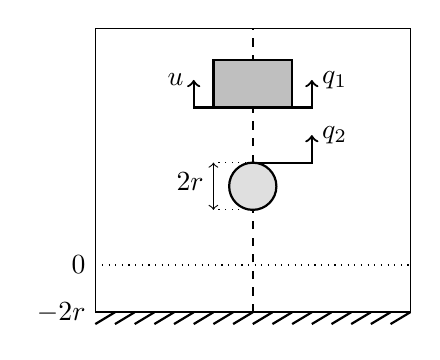
\begin{tikzpicture}
	%
	% axes
	\draw[thick] (0,-0.6)--(4,-0.6);
	\draw[dotted] (0,0) node[anchor = east] {\color{black}$0$}--(4,0);
	\draw[thick,dashed] (2,-0.6) -- (2,3);
	\draw (0,-0.6) node[anchor = east] {$-2r$} -- (4,-0.6) -- (4,3) -- (0,3) -- (0,-0.6);
	
	% robot
	\fill[gray!50, draw = black,thick] (1.5,2) rectangle (2.5,2.6);
	% ball
	\fill[gray!25, draw=black,thick] (2,1) circle (0.3);
	%	
	\draw[thick,->] (2.5,2) -- (2.75,2) -- (2.75,2.35) node[anchor=west] {$q_1$};
	\draw[thick,->] (1.5,2) -- (1.25,2) -- (1.25,2.35) node[anchor=east] {$u$};
	\draw[thick,->] (2,1.3) -- (2.75,1.3) -- (2.75,1.65) node[anchor=west] {$q_2$};
	%
	\draw[dotted] (2,1.3) -- (1.5,1.3);
	\draw[dotted] (2,0.7) -- (1.5,0.7);
	\draw[<->] (1.5,0.7) -- (1.5,1.3)  node[anchor=north east] {$2r$};
	%
	\foreach \x in {0,0.25,0.5,0.75,1,1.25,1.5,1.75,2,2.25,2.5,2.75,3,3.25,3.5,3.75}
	\draw[thick] (\x,-0.75) -- (\x+0.25,-0.6);
\end{tikzpicture}
	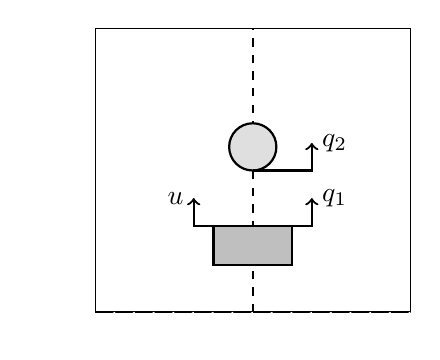
\begin{tikzpicture}
	%
	\draw[thick] (0,-0.6)--(4,-0.6);
	\draw[thick,dashed] (2,-0.6) -- (2,3);
	\draw (0,-0.6)  node[anchor = east] {\color{white}$-2r$} -- (4,-0.6) -- (4,3) -- (0,3) -- (0,-0.6);
	
	% robot
	\fill[gray!50, draw = black,thick] (1.5,0) rectangle (2.5,0.5);
	% ball
	\fill[gray!25, draw=black,thick] (2,1.5) circle (0.3);
	%	
	\draw[thick,->] (2.5,0.5) -- (2.75,0.5) -- (2.75,0.85) node[anchor=west] {$q_1$};
	\draw[thick,->] (1.5,0.5) -- (1.25,0.5) -- (1.25,0.85) node[anchor=east] {$u$};
	\draw[thick,->] (2,1.2) -- (2.75,1.2) -- (2.75,1.55) node[anchor=west] {$q_2$};
	\foreach \x in {0,0.25,0.5,0.75,1,1.25,1.5,1.75,2,2.25,2.5,2.75,3,3.25,3.5,3.75}
	\draw[color = white] (\x,-0.755) -- (\x+0.25,-0.6);
\end{tikzpicture}
	\caption[One--dimensional ball--dribbling and ball--juggling robotic systems.]{One--dimensional ball--dribbling (left) and ball--juggling (right) robotic systems. The position of the robot (rectangle), is represented by the variable $q_1$ while $u$ is an input force applied to it. The position of the ball (circle), of radius $r$, is represented by $q_2$. The ball--juggling system presents a single impact, i.e. the one between the robot and the ball. The ball--dribbling system, instead, is characterized by two impacts: ball--robot and ball--ground.}
	\label{fig:1D}
	%
\end{figure}
%
%%%%%%%%%%%%%%%%%%%%%%%%%%%%%%%%%%
\subsection{Beyond Robot Control}
It has been proven that a novel unified framework for controlling highly dynamic robotic tasks is needed but cannot be approached in a systematic general way due to the \textit{nonsmooth} nature of the robotic tasks.
%
\newline

%
However, many control systems presents discontinuities and multimodality due to the control algorithm itself rather then physics. 
For example, a system subjected to a \textit{sliding--mode controller} \citep{pisano2011sliding} is, technically speaking, an hybrid system. Moreover, the whole framework of \textit{switching control} belongs to field of hybrid dynamical systems.
%
\newline

%
Very simple practical example of how a controller give an hybrid nature to dynamical systems, are the temperature regulator of a room or the water--level control in tanks.
%
\newline
    
%
In the light of this considerations, it is legitimate pose the following questions: \newline
\textit{Can hybrid control systems be modeled from an energetic point of view in port--Hamiltonian fashion?}\newline
\textit{If yes, which theoretical advantages would this formulation give?}

%%%%%%%%%%%%%%%%%%%%%%%%%%%%%%%%%%%%%%%
\subsection{The Identification Problem}
%
As common in Automatic Controls, controller design, simulations and diagnostics of hybrid dynamical systems require an accurate knowledge of the model. However, these {processes} are always characterized by sets of parameters which are typically not available.
%
\newline

%
System identification techniques are the interface between real world application and mathematical world of control theory and mathematical abstraction~\citep{LJUNG20101}. These methods aim to obtain estimates of the parameters and update the model from direct measurements collected during the time evolution of the system~\citep{soderstrom2018errors,SODERSTROM2019}.
%
\newline

%
Dealing with robotic systems, it is well known that inertial parameters must often be thoroughly estimated with well designed identification experiments. Moreover, if the robot experiences impacts or sudden state changes, it is intuitive to understand that further parameters given by the hybrid part of the system must also be estimated. 
Thus, in order to implement any robot controllers for highly dynamic tasks, it is necessary to solve the identification problem first.
%
\newline

%
The majority of the literature on identification of hybrid systems is related to classes of (discrete--time) Piece Wise Affine systems (PWA), i.e. systems which are defined by subdividing the  space into polyhedral regions which have associated an affine state update equation \citep{Bemporad,Ferrari,Juloski,juloski2005bayesian,Paoletti}.
% 
\newline

%
Besides, the identification of hybrid dynamical system in the form of \textit{hybrid inclusions} has to be explored yet. In fact, a systematic identification procedure for this class of systems currently is still missing. Note that, many of the robotics tasks discussed above can be modeled within this framework.
%
\newline

%
Real implementation of those tasks would undoubtedly require the knowledge of some parameters of the plant. Thus, if a novel unified modeling framework merging port--Hamiltonian and hybrid systems is proposed alongside new control techniques, the systematic estimation of physical parameters of both continuous (e.g. mass, inertia, friction) and discrete (e.g. impact restitution coefficient) parts of models  will be needed.
%
\clearpage
%%%%%%%%%%%%%%%%%%%%%%%%%%%%%%%%%%%%%%%%%%%%%%%%%%%%%%%%%%%%%%%%%%%%%%%%%%%%%%%

\section{{Aims and Objectives}}\label{sec:aim}
The aim of this thesis is to present a novel control theoretical framework for physical systems with nonsmooth and multimodal behaviors, with a special insight toward robot control tasks where the current--state--of--the--art approaches fail.

The main objectives are:
%
\begin{itemize}
    \item [1.] \textbf{to develop a novel control theoretical framework by merging the theories of port--Hamiltonian systems and hybrid systems}.
    
    With the aim of solving a robot control problem, the theory of \textit{hybrid port--Hamiltonian systems} is developed combining the theories of port--Hamiltonian systems and \textit{hybrid inclusions}, one of the most general representations of hybrid dynamical systems.
    \newline
    %
    \item [2.] \textbf{to apply the developed theory to a robot control task and prove its effective within the robotics framework}. 
    
    Considering the ball--dribbling robot problem, a novel controller, the \textit{iterative energy shaping} is systematically synthesized, proving the capabilities of the proposed framework.
    \newline
    %
    \item [3.] \textbf{to demonstrate how the developed theory goes beyond robotics and can be used to model a broad variety of control systems}. 
    
    A novel nonlinear hybrid controller for linear time--invariant system is derived from passivity--based techniques, and then this purely control theoretical problem is expressed via hybrid port--Hamiltonian systems.
    \newline
    %
    \item[4.] \textbf{to derive a new systematic identification procedure for a class of hybrid systems}.
    
    As most of hybrid control systems (including the proposed ones) require some knowledge of the physical parameters of the controlled plant, a new systematic procedure is presented to solve the estimation problem. This method can be applied to a variety of hybrid port--Hamiltonian systems 
    
    \end{itemize}
%





%
\clearpage
%%%%%%%%%%%%%%%%%%%%%%%%%%%%%%%%%%%%%%%%%%%%%%%%%%%%%%%%%%%%%%%%%%%%%%%%%%%%%%%

\section{Thesis Content and Structure}
\subsection{Thesis Outline}
This thesis is structured in seven chapters which implement the aim described in \ref{sec:aim}. 
These seven chapter can be logically clustered in four main parts: Introduction and background, theoretical results, applications and conclusions. In line with the objectives, a detailed structure of this thesis is shown in Figure \ref{fig:ThesisStructure}.
%
\newline

%
\textbf{Chapter 1} describes the main motivations, purpose and approach of this study.
%
\newline

%
\textbf{Chapter 2} briefly introduces the fields of port--Hamiltonian systems and hybrid dynamical systems. Throughout the chapter, several illustrative examples related to robotics, mathematical biology and physics are provided to highlight the practical importance of the presented theoretical concepts. 

In the first half of the chapter, the input--state--output model of a port-Hamiltonian system is derived and its most relevant properties are described. Moreover, the basic theory of the energy--balancing passivity--based control is also presented. In the second part of the chapter, the basic results on hybrid systems are introduced. In particular, it will be focused on the class of \textit{hybrid inclusions} and its stability/passivity theory.  The chapter concludes with a summary of the previous attempts to merge the two frameworks and their main limitations. 
%
\newline

%
\textbf{Chapter 3} deals with the definition and characterization of hybrid-port Hamiltonian systems. Starting from the concepts revised in the previous chapter, the new framework is here consistently developed. First, the basic assumptions are stated and the hybrid port--Hamiltonian model is derived. The concept of passivity is subsequently extended to the new model. Necessary and sufficient conditions for passivity are also reported and proved. Then, Lyapunov stability is extended from the one for hybrid inclusions. Finally, all the previous results are used to transfer to the hybrid case some of the features of passivity--based control for port--Hamiltonian systems. As for Chapter 2, application examples will be provided throughout the chapter.
%
\newline

%
\textbf{Chapter 4} introduces the first real application of the developed theory. In particular, the problem of modeling and control a ball--dribbling robot is considered. The main challenges offered by this systems are: under-actuation, dynamic decoupling between the robot and the ball and impacting interactions. First, the system is consistently modeled in hybrid port--Hamiltonian form. Then, a novel energy--based controller is derived from physical intuitions on the system. This controller enhance the classic energy shaping with the iterative learning, allowing the robot to rhythmically bounce the ball at a desired height. Simulations are performed to prove the effectiveness and robustness of the controller.   
%
\newline

%
\textbf{Chapter 5} considers the problem of controlling a linear time--invariant system with a finite number of set points. At first, a nonlinear passive controller is used to stabilize simultaneously all the desired set points. Then, a hybrid optimal impulse controller is designed to switch the between the set points. Numerical simulations are carried out for a mechanical system, proving the results. Alongside the theoretical relevance of the developed control technique, it is finally shown how the controlled system can be modeled as hybrid port--Hamiltonian system, implicitly inheriting some useful properties to analyze its behaviour.
%
\newline

%
\textbf{Chapter 6} proposes a new systematic approach for the identification of a class of hybrid dynamical systems. The main challenge offered by the considered class of systems is the detection of state discontinuities from a time series of state measurements. The proposed solution is based on the analytical computation of an upper bound on the numerically computed time--derivative of the state, above which the system is considered to be ``jumping''. After implementing the jump detection function, the parameters of the system are estimated recursively. Simulations are performed on a mechanical systems to show the effectiveness of the proposed method.
\newline

%
\textbf{Chapter 7} presents the conclusions of this study and future work.
%
\begin{figure}[b]
    \centering
    \definecolor{darkspringgreen}{rgb}{0.09, 0.45, 0.27}
    \tikzstyle{container} = [rectangle, draw, semithick, rounded corners,
                     text width=44mm, minimum height=11mm, align=center,
                     fill=white, drop shadow, inner sep=0.6cm]
    \begin{tikzpicture}[
        node distance = 5mm and 4mm,
        %every node/.style = {font=\bfseries\itshape},
        chapter/.style = {rectangle, draw, semithick, rounded corners,
                     text width=44mm, minimum height=9mm, align=center,
                     fill=white, drop shadow},  
                     ys/.style = {yshift=-5mm}         
                    ]
        \draw[thick] (0,0)  coordinate (A1)
                    node[below right] {Preliminaries \& Background} 
                    -- + (\textwidth,0)
                    coordinate (B1);
        \node (ch1) [chapter, below=of $(A1)!0.5!(B1)$]         {\textbf{Chapter 1}\\ \textit{Introduction}};
        \node (ch2a) [chapter, below  left=1.5cm and -2cm of ch1] {Port--Hamiltonian Systems};
        \node (ch2b) [chapter, below right=1.5cm and -2cm of ch1] {Hybrid Dynamical Systems};
        \node [container,fit=(ch2a) (ch2b), yshift = 0.5cm] (c1) {\textbf{Chapter 2}\\ \textit{Preliminaries}\textcolor{white}{\\aa\\aa}};
        \node (ch2a) [chapter, below  left=1.5cm and -2cm of ch1] {Port--Hamiltonian Systems};
        \node (ch2b) [chapter, below right=1.5cm and -2cm of ch1] {Hybrid Dynamical Systems};
        %
        \draw[thick] ([ys] A1 |- ch2a.south)  coordinate (A2)
                    node[below right] {Theoretical Results}
                    -- + (\textwidth,0)
                    coordinate (B2);
        \node (ch3) [chapter, below=of $(A2)!0.5!(B2)$,text width=54mm, fill = gray!50]   {\textbf{Chapter 3}\\\textit{Hybrid Port--Hamiltonian Systems}};
        %\node (ch3) [chapter, below  left=of $(A2)!0.5!(B2)$]   {State of the Art};
        %\node (ch4) [chapter, below right=of $(A2)!0.5!(B2)$]   {Building of Theory};
        \draw[thick] ([ys] A1 |- ch3.south)  coordinate (A3)
                    node[below right] {Applications}
                    -- + (\textwidth,0)
                    coordinate (B3);
        \node (ch4) [chapter, below=of $(A3)!0.5!(B3)$,text width=84mm, fill = gray!50] {\textbf{Chapter 4}\\\textit{Iterative Energy shaping of a Ball--dribbling Robot}};
        \node (ch5) [chapter, below=of ch4,text width=84mm, fill = gray!50]                     {\textbf{Chapter 5}\\\textit{Multistable Energy Shaping with Hybrid Mode Selector}};
        \node (ch6) [chapter, below=of ch5,text width=84mm, fill = gray!50]                     {\textbf{Chapter 6}\\\textit{Identification of a Class of Hybrid Systems}};
        \draw[thick] ([ys] A1 |- ch6.south)  coordinate (A4)
                    node[below right] {Conclusion}
                    -- + (\textwidth,0)
                    coordinate (B4);
        \node (ch7) [chapter, below=of $(A4)!0.5!(B4)$]         {\textbf{Chapter 7}\\Discussion and conclusions};
        %\node (ap1) [chapter, below  left=of ch7]               {\textbf{Appendix A}};
        %\node (ap2) [chapter, below =of ch7]                    {\textbf{Appendix B}};
        %\node (ap3) [chapter, below right=of ch7]               {\textbf{Appendix C}};
        %
        \draw [-latex, ultra thick, blue] (ch1)--(c1);
        \draw [-latex, ultra thick, blue] (ch2a.south) to[out=-45,in=90] (ch3.north);
        \draw [-latex, ultra thick, blue] (ch2b.south) to[out=-135,in=90] (ch3.north);
        \draw [-latex, ultra thick, blue] (ch3.south) to[out=-90, in=90] (ch4.north);
        \draw [-latex, ultra thick, blue] (ch3.south) to[out=-155,in=130,distance=3.5cm] (ch5.west);
        \draw [-latex, ultra thick, red] (ch2b.south) to[out=-45,in=30,distance=2.5cm] (ch6.east);
        \draw [-latex, ultra thick, darkspringgreen] (ch6.south)--(ch7.north);
        \draw [-latex, ultra thick, darkspringgreen] (ch5.west) to[out=200,in=180,distance=1.5cm] (ch7.west);
        \draw [-latex, ultra thick, darkspringgreen] (ch4.west) to[out=200,in=180,distance=3cm] (ch7.west);
    \end{tikzpicture}
    \vspace{5mm}
    \caption[Thesis outline.]{Thesis outline. The coloured arrows indicate the logical flows of the contents throughout the thesis, highlighting, e.g., how the theory presented in the first chapters is employed in the various applications. Chapters in light gray blocks contain exclusively original content developed by the author,}
    \label{fig:ThesisStructure}
\end{figure}
%
%\newline
%
%
\subsection{Thesis Content}
This thesis is developed across three main broad fundamental fields: control theory, robotics and statistics. The Venn diagram in Fig. \ref{fig:venn} clarifies how the contents are interconnected within the main research fields. In particular, the first three chapters are related to pure control as port--Hamiltonian systems and hybrid dynamical systems are firstly introduced in Chapter 2 and then merged in Chapter 3. Chapter 5 is also mostly related to theoretical aspects. However, the concepts of Chapter 4, which introduces the ball--dribbling robot encompasses the intersection of control theory and robotics with . Chapter 6 treats the parameters estimation problem for a class of hybrid dynamical systems, spanning in the intersection of control theory and statistics.

\begin{figure}
    \centering
    \def\firstcircle{(0,0) circle (2.5cm)}
    \def\secondcircle{(45:3.5cm) circle (2.5cm)}
    \def\thirdcircle{(0:4.5cm) circle (2.5cm)}
    \def\id{(3,-2.5) ellipse (0.65 and 0.65)}
    \def\hds{(3,-1.3) ellipse (1.5 and 1.2)}
    \def\ph{(3.2,0) ellipse (1.5 and 1.2)}
    \definecolor{carminered}{rgb}{1.0, 0.0, 0.22}
    \definecolor{cerulean}{rgb}{0.0, 0.48, 0.65}
    \definecolor{bluegray}{rgb}{0.4, 0.6, 0.8}
    \definecolor{amber}{rgb}{1.0, 0.75, 0.0}
    \definecolor{emerald}{rgb}{0.31, 0.78, 0.47}
    %
    \begin{tikzpicture}
        \draw[thick, fill=gray!30,fill opacity=0.3] \firstcircle;
        \draw[thick, fill=gray!30,fill opacity=0.3] \secondcircle node [above] {};%{\small Control Theory};
        \draw[thick, fill=gray!30,fill opacity=0.3] \thirdcircle node [below] {};%{Statistics};
        \draw[thick, fill=gray!50,fill opacity=0.4, rotate = 60] \hds node [below] {};%{Statistics};
        \draw[thick, fill=gray!50,fill opacity=0.4, rotate = 60] \ph node [below] {};%{Statistics};
        \draw[thick, fill=gray!50,fill opacity=0.4, rotate = 60] \id node [below] {};%{Statistics};
        %
        \begin{scope}[rotate = 60]
            \clip \hds;
            \draw[thick, fill = amber] \ph;
        \end{scope}
        %
        \begin{scope}[rotate = 60]
            \clip \hds;
            \clip \firstcircle;
            \draw[-,black,thick, fill = bluegray] \ph;
        \end{scope}
        %
        \begin{scope}[rotate = 60]
            \clip \hds;
            \fill[emerald] \id;
        \end{scope}
        %%%%%%%%%%%%
        \draw (0,0)   node[]{\textbf{Robotics}};
        \draw (0:4.5) node[]{\textbf{Statistics}};
        \draw (2.55,4.45) node[]{\textbf{Control Theory}};
        \draw (-1,4.75) node[] (ph) {Port--Hamiltonian Systems};
        \draw (7.25,3.25) node[] (hds) {Hybrid Dynamical Systems};
        \draw (8,2) node[] (id) {System Identification};
        %
        \draw[-o, thick] (ph.south) to[out = -90,in = 150] (1.5,3);
        \draw[-o, thick] (hds.south) to[out = -90,in = 50] (3.5,2.5);
        \draw[-o, thick] (id.south) to[out = -90,in = -50] (3.85,1.25);
        %%%
        \draw (-1,-3) node[] (ch4) {\color{amber}\textbf{Chapter 4}};
        \draw (3,-3) node[] (ch5) {\color{bluegray}\textbf{Chapter 5}};
        \draw (7,-3) node[] (ch6) {\color{emerald}\textbf{Chapter 6}};
        %
        \draw[-o, dashed, thick] (ch4.north) to[out = 45,in = 180, distance = 4cm] (2.35,2.5);
        \draw[-o, dashed, thick] (ch5.north) to[out = 110,in = 250] (1.6,1.75);
        \draw[-o, dashed, thick] (ch6.north) to[out = 120,in = 250, distance = 3cm] (3.4,1.5);
    \end{tikzpicture}
    \vspace{5mm}
    \caption[Venn diagram of the contents presented in this thesis.]{Venn diagram of the contents presented in this thesis. In particular, Chapters 3 and 5 are related to theoretical aspects of hybrid port--Hamiltonian systems. Chapter 4 presents the application of hybrid port--Hamiltonian systems to robotics. Finally, Chapter 6 deals with the identification of hybrid systems, located in the meeting point of control theory and statistics.}
    \label{fig:venn}
\end{figure}

\clearpage
%%%%%%%%%%%%%%%%%%%%%%%%%%%%%%%%%%%%%%%%%%%%%%%%%%%%%%%%%%%%%%%%%%%%%%%%%%%%%%%

%\the\textwidth = 379.37pt

\chapter{Preliminaries}
%Related research
\label{chap:preliminaries}
\minitoc

\thispagestyle{empty}

\newpage
\definecolor{brickred}{rgb}{0.8, 0.25, 0.33}
%
%%%%%%%%%%%%%%%%%%%%%%%%%%%%%%%%%%%%%%%%%%%%%%%%%%%%%%%%%%%%%%%%%%%%%%%%%%%%%%%
\section{Introduction\label{sec:2_intro}}
\lettrine[lines=4]{\color{brickred}T}{his} chapter presents a brief introduction of the fundamental theories which are employed to develop the whole thesis, i.e. the ones of \textit{port--Hamiltonian systems} and \textit{hybrid dynamical systems}. The inclusion of this Chapter in this thesis is justified by the need of smoothly introducing the reader -- which might not be an expert on control theory -- to the very basic concepts which will be used intensively in the rest of the manuscript.
%
\newline

%
At first, the concept of Lyapunov stability and passivity are recalled together with some of the properties of passive system, e.g. output feedback stabilization.
%
\newline

%
Then the input--state--output model of a port--Hamiltonian (PH) system is defined. Then, it is shown how the power balance equation, derived from the model, highlights the most important properties of this framework. Three modeling examples are provided to give a physical and practical meaning to the theory. The first two examples are related to the dynamics of mechanical systems while the third one is taken from mathematical biology, proving the generality of the PH framework.   
The passivity--based control of port--Hamiltonian system is then briefly treated, showcasing the popular \textit{energy--balancing} technique. Both theoretical and numerical examples are given. 
%
\newline

%
The second part of the Chapter deals with hybrid dynamical systems, their \textit{hybrid inclusions} specialization and the basic stability properties of this type of systems. First, the definition of hybrid inclusion is provided alongside the concept and parametrization of the solutions of this type of models. Then, several examples are provided to consolidate the theory. Finally, the Lyapunov stability theorem for hybrid inclusions is enunciated and applied to the previous examples. 
%

\clearpage
%%%%%%%%%%%%%%%%%%%%%%%%%%%%%%%%%%%%%%%%%%%%%%%%%%%%%%%%%%%%%%%%%%%%%%%%%%%%%%%
%\section{Stability and Passivity}

\subsection{Stability of Autonomous Systems}
%
Consider an autonomous time--invariant nonlinear dynamical system
%
\begin{equation}\label{eq:nlsys}
    \dot{\xb} = \mathbf{f}(\xb)
\end{equation}
%
where $\mathbf{f}:\R^n\supseteq\X\rightarrow\R^n$ is assumed smooth enough such that solutions are forward complete for all initial conditions $\xb_0\in\X$. Let $\xb^*$ be a fixed point of (\ref{eq:nlsys}).
%
\begin{defn}[Lyapunov Stability \citep{khalil2002nonlinear}]
    The equilibrium point $\xb^*$ of (\ref{eq:nlsys}) is 
    \begin{itemize}
        \item stable if
            \begin{equation}
                \forall \varepsilon>0 ~~  \exists \delta_\varepsilon>0~:~\|\xb_0 - \xb^*\|_2 <\delta_\varepsilon \Rightarrow \|\xb(t) - \xb^*\|_2<\varepsilon.
            \end{equation}
            \item asymptotically stable if
            \begin{equation}
                \exists \delta>0~:~\|\xb_0 - \xb^*\|_2<\delta\Rightarrow\lim_{t\rightarrow\infty}\xb(t) =  \xb^*.
            \end{equation}
        \item unstable if it is not stable.
    \end{itemize}
\end{defn}
%
Stability in the sense of Lyapunov of a system in the form (\ref{eq:nlsys}) can be addressed using Lyapunov's Second theorem.
%
\begin{thm}[Lyapunov's Second Theorem \citep{khalil2002nonlinear}]\label{thm:lyap_nl}
    Let $\xb^*$ be a fixed point for (\ref{eq:nlsys}) and $\xb^*\in\A\subset\R^n$. Let $V:\A\rightarrow\R$, $V\in\C_1^n$ such that
    %
    \begin{align}
        & \forall \xb\in\A\setminus\xb^* && V(\xb)>0~~\text{and}~~V(\xb^*) = 0,&\\
        & \forall \xb\in\A & &\dot{V}(\xb)\leq 0,&
    \end{align}
    %
    then $\xb^*$ is stable. Furthermore, if
    %
    \begin{align}
        \forall \xb\in\A \setminus\xb^* ~~~ \dot{V}(\xb)< 0,
    \end{align}
    %
    then $\xb^*$ is asymptotically stable.
\end{thm}
%
%%%%%%%%%%%%%%%%%%%%%%%%%%%%%%%%%%%%%%%%%%%%%%%%%%%%%%%%%%%%%%%%%%%%%%%%%%%%%%%%%%%%%%%%%%%%%%%%%%%%%%%%%%
\clearpage
\subsection{Passivity: Basic Definitions}
%
Let us consider a controlled affine system:
\begin{equation}\label{eq:nlaffine}
    \left\{
    \begin{matrix*}[l]
        \dot{\xb} = \fb(\xb) + \gb(\xb)\ub\\
        \yb = \hb(\xb)
    \end{matrix*}
    \right.
\end{equation}
where $\xb\in\X\subset\R^n$, $\ub\in\U\subset\R^m$, $\yb\in\Y\subset\R^m$. $\fb:\X\rightarrow\R^n$, $\gb:\X\rightarrow\R^{m\times n}$ ($\rank(\gb)= m\leq n$) and $\hb:\X\rightarrow\R^m$ are assumed smooth enough such that the solutions are forward--complete for all initial conditions $\xb_0\in\X$ and all inputs $\ub(t)\in\mathcal{L}_2^m$. Let $\bm\phi(t,\xb_0,\ub)$ denote the state trajectory at time $t\geq0$.
%
A \textit{supply rate} is a real valued function $w$ defined on $\Y\times\U$. The  system (\ref{eq:nlaffine}) is said to be \textit{dissipative} with respect to the supply rate $w$ if there exists a continuous function $\Ha:\X\rightarrow\R^+$, called \textit{storage function} such that, for all $\ub\in\U$, $\xb\in\X$ and $t\geq 0$, it holds
%
\begin{equation}
    \Ha(\xb(t))-\Ha(\xb(0)) \leq \int_0^tw(s)ds.
\end{equation}
%
Furthermore, the system is said to be \textit{passive} if it is dissipative with respect to the supply rate $w = \langle \yb,\ub \rangle$. The supply rate $w$ and the storage function $\Ha(\xb)$ can be thought as the generalized power and the generalized energy\footnote{Without any loss of generality, $\Ha(\xb)$ can be taken bounded from below rather than nonnegative, since the properties of storage functions hold regardless of an additive constant.}, respectively. In fact, the pair $(\ub,\yb)$ represents the medium by which the system can exchange generalized energy through $w$ \citep{secchi2007control}.
%
\begin{defn}(Kalman-Yakubovich-Popov (KYP) Property).
    %
    System (\ref{eq:nlaffine}) is said to enjoy the KYP property if there exists a storage function $\Ha:\X\rightarrow\R^+$, $\Ha(\xb)\in\mathcal{C}^1$, $\Ha(\mymathbb{0}_n) = 0$ such that:
    \begin{equation}
        \left\{
        \begin{matrix*}[l]
            {\dH(\xb)}\fb(\xb)\leq 0\quad\\ 
            {\dH(\xb)}\gb(\xb)= \hb^\top(\xb)
        \end{matrix*}
        \right.
    \end{equation}
    %
    for all $\xb\in\X$.
    %
\end{defn}
%
It is worth noticing that ${\dH(\xb)}\fb(\xb)$ is the natural dissipation of the system while ${\dH(\xb)}\gb(\xb)\ub(t)=\yb^\top(t)\ub(t)$ is the instant power flow at time $t$.
%
\begin{prop}[\citealp{byrnes91}]
    %
    System (\ref{eq:nlaffine}) is passive with storage function $\Ha(\xb)\in \mathcal{C}^1$ if and only if it enjoys the KYP property.
    %   
\end{prop}
%
\begin{rem}\textcolor{white}{a}
\begin{itemize}
    \item[i)] Dissipative (and thus passive) systems have no internal production of generalized energy, only its dissipation is possible; 
    \item[ii)] Moreover, the total amount of generalized energy that can be extracted from a dissipative system is bounded from above by the amount that is initially stored; 
    \item[iii)] Strict minima of $\Ha$ corresponding to fixed points of (\ref{eq:nlaffine}) are Lyapunov stable, as it can be deduced comparing the KYP Property with Theorem \ref{thm:lyap_nl}.
\end{itemize}
\end{rem}
%
%%%%%%%%%%%%%%%%%%%%%%%%%%%%%%%%%%%%%%%%%%%%%%%%%%%%%
\subsection{Output Feedback Stabilization of Passive Systems}\label{sec:OutFeedStab}
%
\begin{defn}[Observability]
	A system (\ref{eq:nlaffine}) is locally zero state observable if there exists a neighborhood $\B\subset\X$ such that
	% 
	\begin{equation}
	    \forall \xb\in \B,~\forall t\geq 0 \quad \hb(\bm\phi(t,\xb,\mymathbb{0}_m))=\mymathbb{0}_n~~\Rightarrow~~ \xb=\mymathbb{0}_n
	\end{equation}
	%
	If $\B\equiv\X$ the system is said zero state observable.
\end{defn}

\begin{defn}[Detectability]
	A system (\ref{eq:nlsys}) is locally zero state detectable if there exists a neighborhood $\B\subset\X$ of $\mymathbb{0}_n$ such that,
	% 
	\begin{equation}
	    \forall \xb\in \B,~\forall t\geq 0 \quad \hb(\bm\phi(t,\xb,\mymathbb{0}_m))=\mymathbb{0}_n~~\Rightarrow~~ \lim\limits_{t\rightarrow\infty}\bm\phi(t,\xb,\mymathbb{0}_m)=\mymathbb{0}_n
    \end{equation}
	%
	If $\B\equiv\X$ the system is said zero state detectable.
\end{defn}
%
%
\begin{defn}[Radially Unbounded (Proper) Function]
	A nonnegative function $\Ha:\X\rightarrow\R^+$ is a radially unbounded (proper) function if
	\begin{equation}
	\forall r\in\R^{*,+}\quad  \left\{\xb\in\X~:~0\leq \Ha(\xb)\leq r \right\}
	\end{equation}
	%
	is compact.
\end{defn}
%
A basic stabilization property of passive system is given by the following theorem, whose proof is closely related to the La Salle's invariance principle \citep{lasalle1960some}. 
%
\begin{thm}[Output Feedback Asymptotic Stabilization \citep{byrnes1991passivity}]
	Consider a passive system (\ref{eq:nlaffine}):
	%
	\begin{itemize}
	    \item[i)] with a fixed point $\xb^*=\mymathbb{0}_n$;
	    \item[ii)] with positive definite storage function $\Ha$;
	    \item[iii)] locally zero state detectable.
	\end{itemize}
	%
	Let $\bm\alpha:\Y\rightarrow\U$ be a smooth function such that 
	%
	\begin{equation}
	    \bm\alpha(\mymathbb{0}_m)=\mymathbb{0}_m~~\land~~ \forall \yb\in\Y\setminus\{\mymathbb{0}_m\}~~~~\yb^\top\bm\alpha(\yb)>0.
	\end{equation}
	%
	The control law:
	%
	\begin{equation}\label{eq:ofs}
	\ub=-\bm\alpha(\yb)
	\end{equation}
	%
	asymptotically stabilizes the equilibrium point.
	%
\end{thm}
%
\begin{cor}
    If the system is zero state detectable and $\Ha$ is radially unbounded, then the control law (\ref{eq:ofs}) globally asymptotically stabilizes the system.
\end{cor}
%
Applying a change of coordinates, it can be shown that any strict minimum of the storage function can be (locally) asymptotically stabilized by the output feedback (\ref{eq:ofs}).
%
\newline

%
It is also possible to show that an analogous result holds without explicitly assuming the zero-state detectability of the nonlinear system.
\begin{prop}[\citealp{macchelli2003port}]
	If (\ref{eq:nlaffine}) is passive with positive definite storage function $\Ha$, the control law $\ref{eq:ofs}$ (locally) asymptotically stabilizes $\xb=\mymathbb{0}_n$, if, given a neighborhood $\B_0$ of $\x=\mymathbb{0}_n$, the largest invariant set contained in
	%
	\begin{equation*}
		\left\{\xb\in\X\cap\B_0~:~\yb(\xb)=\mymathbb{0}_m\right\}
	\end{equation*}
	%
	is $\{\mymathbb{0}_n\}$.
\end{prop}
%
The final result recalled in this section will be one of the most useful in the sect Sections and Chapters.
%
\begin{cor}\label{th:ofgs}
	Suppose that a system (\ref{eq:nlaffine}) with $\xb=\mymathbb{0}_n$ as afixed point, is passive with a $\mathcal{C}^1$ proper positive definite storage function $\Ha$. If the system is zero--state observable then, $\forall\mathbf{K}\succ 0$, the control law
	%
	\begin{equation}
	    \ub=-\mathbf{K}\yb
	\end{equation}
	%
	globally asymptotically stabilizes the equilibrium point.
\end{cor}
%
\clearpage
%%%%%%%%%%%%%%%%%%%%%%%%%%%%%%%%%%%%%%%%%%%%%%%%%%%%%%%%%
\section{Port--Hamiltonian Systems\label{sec:PH_systems}}
%
%Port--Hamiltonian (PH) systems has been introduced in ...
%
\subsection{Input--State--Output Model}
%
The input--state--output representation of a port-Hamiltonian system is
%
\begin{equation}\label{eq:PHsys}
	\left\{
	    \begin{matrix*}[l]
	        \dot{\xb} = \left[\mathbf{J}(\xb) - \mathbf{R}(\xb)\right]\bm{\nabla}\Ha(\xb) + \mathbf{G}(\xb)\mathbf{u}\\
	        \mathbf{y} = \mathbf{G}^\top(\xb)\bm{\nabla}\Ha(\xb) 
	    \end{matrix*}
	\right.
\end{equation}
%
where $\xb\in\R^n$ is the state of the system, $\ub\in\U\subset\R^m$ is the input and $\yb\in\Y\subset\R^m$ is the output.
Furthermore, the scalar function $\Ha:\R^n\rightarrow\R$ is the Hamiltonian of the system (i.e. its energy), the skew symmetric matrix $\mathbf{J}(\xb) = -\mathbf{J}^\top(\xb)$, $\mathbf{J}\in\R^{n\times n}$ is the interconnection matrix representing power--preserving interconnections related to a Dirac structure. The positive semidefinite matrix $\mathbf{R}(\xb) = \mathbf{R}^\top(\xb)\succeq 0$, $\mathbf{R}\in\R^{n\times n}$ represents dissipative effects in the system while the matrix $\mathbf{G}\in\R^{n\times m}$ ($\rank~ \mathbf{G}(\xb) = m$) represents the power ports.
%
\newline

%
Note that, in general, $\xb\in\X\subset\R^n$ with $\X$ being a $n$--dimensional manifold, $\U$ a $m$--dimensional vector space and $\Y = \U^*$ its \textit{dual space}. Consequently the natural pairing $\langle\ub,\yb\rangle = \yb^\top\ub$ can be defined, which carries the unit measure of power.
%
\newline

%
It is immediate to show that Port--Hamiltonian systems are \textit{passive} by inspecting their power--balance equation. In fact,
%
\begin{align}
    \dot{\Ha} &= \bm{\nabla}^\top\Ha(\x)\dot{\x} \\
              &= \bm{\nabla}^\top\Ha(\x)\left[\mathbf{J}(\xb) - \mathbf{R}(\xb)\right]\bm{\nabla}\Ha(\xb) + \bm{\nabla}^\top\Ha(\x)\mathbf{G}(\xb)\mathbf{u} \\
              &= -\bm{\nabla}^\top\Ha(\x)\mathbf{R}(\xb)\bm{\nabla}\Ha(\xb) + \yb^\top\ub \\
              &\leq \yb^\top\ub.
\end{align}
%
Note that the term $\bm{\nabla}^\top\Ha(\x)\mathbf{R}(\xb)\bm{\nabla}\Ha(\xb)$ is given by the natural (internal) dissipation effects of the system, e.g. friction in mechanical systems, electrical resistance, etc. and it is often denoted as $d(t)$.
%

%
The first direct consequence is that any local minimum $\xb^*$ of $\Ha(\xb)$, i.e.
\begin{equation}
    \xb^*:~~\bm\nabla\Ha(\x^*) = \mymathbb{0}_n~\land~\bm\nabla^2\Ha(\x^*)\succeq 0
\end{equation}
is a Lyapunov stable equilibrium point of the system. Furthermore, $\xb^*$ can be asymptotically stabilized with a proper output feedback law (see Subsection \ref{sec:OutFeedStab}).
%
\textcolor{black}{
\begin{rem}\textcolor{white}{a}
    \begin{itemize}
	\item [1.] The PH description of a physical system underlines the energetic properties of the system: the amount of energy stored, (state energy variables), the energy dissipation (dissipative elements), the interfaces with the external world (power ports) and the interconnection structure through which the parts of the system exchange energy.
	\item [2.] The concepts of port--based modeling have also been extended to distributed parameters systems by \cite{MASCHKE200027,maschke2001hamiltonian} \cite{rodriguez2001stabilization,macchelli2003port,macchelli2004modeling,macchelli2004port2,macchelli2004port}.
    \end{itemize}
\end{rem}}

%
Three examples of port-Hamiltonian modeling are hereafter reported.  
%
\begin{exmp}[Fully--actuated mechanical system]\label{ex:ndof}
    %
	Consider an $n$--degrees--of--freedom fully--actuated mechanical system with Lagrange generalized coordinates $\q\in\Q\subset\R^n$, inertia matrix $\mathbf{M}(\q)$, kinetic energy $\K(\dot{\q})\triangleq\frac{1}{2}\dot{\q}^\top \mathbf{M}(\q)\dot{\q}$ and potential $\V(\q)$. The Lagrangian of the system $\La:\R^n\times\R^n\rightarrow\R$ is
    %
    \begin{equation}
        \La(\q,\dot{\q}) \triangleq  \K(\dot{\q}) - \V(\q)
    \end{equation}
    %
    By defining the generalized momenta conjugated to $\q$ as
    %
    \begin{equation}
        \p \triangleq \frac{\partial \La}{\partial \dot{\q}} = \mathbf{M}(\q)\dot{\q}\in T^*\Q    
    \end{equation}
    %
    an explicit port--Hamiltonian representation of the system can be obtained by defining:
	%
	\begin{align}
	    \x &\triangleq (\q,\p)\in\R^{2n}\\
	    \Ha(\q,\p) &\triangleq\frac{1}{2}\p^\top\mathbf{M}^{-1}(\q)\p + \V(\q)
	\end{align}
	%
	and, at last,
	%
	\begin{align*}
	    %
	    \Jb = \begin{bmatrix}
	        \mathbb{O}_n&\mathbb{I}_n\\
	        -\mathbb{I}_n&\mathbb{O}_n
	    \end{bmatrix}\in\R^{2n\times 2n},~~ &
	    %
	    \Rb(\q,\p) = \begin{bmatrix}
	        \mathbb{O}_n&\mathbb{O}_n\\\mathbb{O}_n&\mathbf{D}(\q,\p)
	    \end{bmatrix}\in\R^{2n\times 2n}, &
	    %
	    \mathbf{G}(\q)=\begin{bmatrix}
	        \mathbb{O}_{n}\\\mathbf{B}(\q)
	    \end{bmatrix}\in\R^{2n\times n} &
	    %
	\end{align*}
	%
	with $\mathbf{D}(\q,\p) = \mathbf{D}^\top(\q,\p)\succeq 0$, which takes into account the dissipation effects (friction). Moreover, since the system is fully actuated, $\ub\in\R^n$, $\mathbf{G}\in\R^{2n\times n}$ and $\rank(\mathbf{G}) = n$.
	
	Physically, inputs represent external forces (torques) and the outputs are joint velocities. The resulting model is the following:
	%
	\begin{equation}\label{eq:nDOF}
	    %
	    \left\{
	        \begin{matrix*}[l]
	        %
	        \begin{bmatrix}	\dot{\q}\\\dot{\p}\end{bmatrix} 
        	=
	        %
	        \begin{bmatrix}\mathbb{O}_n&\mathbb{I}_n\\-\mathbb{I}_n&-\mathbf{D}(\q,\p)\end{bmatrix}
	        %
	        \begin{bmatrix}\bm{\nabla}_{\q}\Ha\\\bm{\nabla}_{\p}\Ha\end{bmatrix}
	        +
	        \begin{bmatrix}\mathbb{O}_n\\\mathbf{B}(\q)\end{bmatrix}\ub\\\\
	        %
	        \yb = \begin{bmatrix}\mathbb{O}_n&\mathbf{B}^\top(\q)\end{bmatrix}\begin{bmatrix}\bm{\nabla}_{\q}\Ha\\\bm{\nabla}_{\p}\Ha\end{bmatrix}
	    \end{matrix*}
	    \right.
	    %
	\end{equation}
	%
	Note that, as expected the natural dissipation of the system (given by friction) becomes
	%
	\begin{align}
	    d(t) &= -\bm{\nabla}_\p^\top\Ha\mathbf{D}(\q,\p)\bm{\nabla}_\p^\top\Ha =\\ &=\p^\top\mathbf{M}^{-1}(\q)\mathbf{D}(\q,\p)\mathbf{M}^{-1}(\q)\p =\\
	    &= \dot{\q}^\top\mathbf{D}(\q,\p)\dot{\q}
	\end{align}
	%
	A graphical representation of the model is provided in Fig. \ref{fig:MECHscheme}.
	%
	\begin{figure}[!ht]
	    \centering
	    %\tikzstyle{block} = [draw, fill=gray!20, rectangle, 
minimum height=1em, minimum width=2em]
\tikzstyle{sum} = [draw, fill=gray!50, circle, node distance=1cm]
\tikzstyle{input} = [coordinate]
\tikzstyle{output} = [coordinate]
\tikzstyle{pinstyle} = [pin edge={to-,thin,black}]
\tikzset{container/.style={draw, rectangle, dashed, inner sep=1.7em }}
	% The block diagram code is probably more verbose than necessary
	\begin{tikzpicture}[auto, node distance=2cm,>=latex']
	% We start by placing the blocks
	\node [input](input){};
	\node [input, right of=input, node distance= 60] (sum) {};
	\node [block, right of=sum, node distance= 30] (int) {$\int$};
	%
    \node[block,below of=int, node distance = 40](int2) {$\int$};
	\node [sum, below of=sum, node distance = 40] (sum2) {};
	
    \node [block, name=G, left of = sum2,  node distance = 30] {$\mathbf{B}(\q)$};
    \node [input,left of=G, node distance= 30,name=u]{};
    \node [block, right of=int2, node distance = 40] (Mi) {$\mathbf{M}^{-1}(\q)$};
    \node [block, below of=Mi, node distance = 20] (D) {$-\mathbf{D}(\q,\p)$};
    \node [block, right of=int, node distance = 40] (V) {$-\bm{\nabla}_\q\V(\cdot)$};
    
    \node [output, right of=V,node distance= 30] (output) {$\q$};
    \node [output, right of=Mi, node distance = 40] (output2) {};
    \node [block, right of=output2, node distance = 30] (B2) {$\mathbf{B}^\top(\q)$};
    \node [output, right of=B2, node distance = 20] (output3) {};
    \node [output, right of=B2, node distance = 40] (output4) {};
    
    
	% Once the nodes are placed, connecting them is easy. 
	\draw [draw,-latex, semithick] (u) -- node {$\mathbf{u}$} (G);
	\draw [draw,-latex, semithick] (G) -- (sum2);
	
	%\draw [-latex] (sum) -- node {$\dot{\q}$} (int);
	\draw [-latex, semithick] (sum2) -- node {\vspace{-10mm} $\dot{\p}$} (int2);
	
	\draw [-latex, semithick] (int) -- node [name=y] {$\q$} (V);
	\draw [-latex, semithick] (int2) -- node [name=y2] {$\p$} (Mi);
    %
	%\draw  node [below of = sum, node distance = 0] (p1) {$+$};
	\draw  node [below of = sum2, node distance = 0] (p2) {$+$};
	
	\draw [-latex, semithick] (Mi) -- (output2) -- node {$\dot{\q}$} (B2);
	\draw [-latex, semithick] (output2) |- (D) -| (sum2);
	%\draw [-latex] (output2) |-(temp) -| (sum);
	\draw [-latex, semithick] (output2) to[out = 90, in = -90, distance = 1cm] (int);
	\draw [-latex, semithick] (V) to[out = -0, in = 90, distance = 3.5cm] (sum2);
	\draw [-latex, semithick] (output3) to[out = -45, in = -135, distance = 3cm] (sum2);
	\draw [-latex, semithick] (B2) -- node {$\yb$} (output4);
\end{tikzpicture}
	    \caption[Block diagram of the port-Hamiltonian model of a fully--actuated $n$--degrees of freedom mechanical systems.]{Block diagram of the port-Hamiltonian model of a fully--actuated $n$--degrees of freedom mechanical systems. The diagram can be easily obtained from equation (\ref{eq:nDOF}) recognizing that $\bm{\nabla}_\q\Ha = \bm{\nabla}_\q\V(\q)$ and $\bm{\nabla}_\p\Ha = \mathbf{M}^{-1}(\q)\p$.}
	    \label{fig:MECHscheme}
	\end{figure}
	%
\end{exmp}
%
The linear specialization of the previous example will be now introduced in order to show some numerical simulations.
%
\begin{exmp}[Mass--spring--damper system]\label{ex:msd}
    Consider the mass--spring--damper system represented by Figure \ref{fig:msd} where $q$ indicates the absolute position of the mass, $k$ is the stiffness of the spring and $b$ is the damping coefficient of the dashpot. Moreover, let $m$ be the mass of the cart and $p = m\dot{q}$ its momentum. 
    %
    \begin{figure}[!ht]
	    \centering
	    %% \begin{tikzpicture}
% \tikzstyle{spring}=[thick,decorate,decoration={zigzag,pre length=0.3cm,post length=0.3cm,segment length=6}]
% \tikzstyle{damper}=[thick,decoration={markings,  
% 	mark connection node=dmp,
% 	mark=at position 0.5 with 
% 	{
% 		\node (dmp) [thick,inner sep=0pt,transform shape,rotate=-90,minimum width=15pt,minimum height=3pt,draw=none] {};
% 		\draw [thick] ($(dmp.north east)+(2pt,0)$) -- (dmp.south east) -- (dmp.south west) -- ($(dmp.north west)+(2pt,0)$);
% 		\draw [thick] ($(dmp.north)+(0,-5pt)$) -- ($(dmp.north)+(0,5pt)$);
% 	}
% }, decorate]
% \tikzstyle{ground}=[fill,pattern=north east lines,draw=none,minimum width=0.75cm,minimum height=0.3cm,inner sep=0pt,outer sep=0pt]

% %\node [style={draw,outer sep=0pt,thick}] (M) [minimum width=1.5cm, minimum height=1cm] {$m$};

% %\node [circle] (M) [minimum width=1.5cm, minimum height=1cm] {$m$};
% \node[style={draw=blue,thick,circle,inner sep=0pt}, minimum size=0.5cm, color=black](M){$m$};; 
% \node (ground) [ground,anchor=north,yshift=-0.5cm,minimum width=5.6cm,xshift=-0.03cm] at (M.south) {};
% \draw (ground.north east) -- (ground.north west);
% \draw (ground.south east) -- (ground.south west);
% \draw (ground.north east) -- (ground.south east);
% \draw (ground.north west) -- (ground.south west);

% \draw [spring] (-1.3,-1.27) -- (-1.3,0);
% \node (k) at (-1.2,-1.27) [xshift = -.4cm,yshift = .8cm] {$a$};
% %
% \draw [damper] (1.3,-1.27) -- (1.3,0) ;
% \node (b) at (1.2,-1.27) [xshift = .6cm,yshift = .8cm] {$b$};
% %
% \draw [thick] (-1.315,0)--(-.75,0);
% \draw [thick] (1.315,0)--(.75,0);
% %\draw [thick] (-2.5,1)--(-2.5,2);
% %\draw [thick] (-0.8,1)--(-0.8,2);
% %\draw [thick] (0,0.5)--(0,1.5);
% %\draw [thick] (-0.8,1.5)--(0,1.5);

% %\draw [-latex,ultra thick] (M.north) ++ (0cm,0cm) -- +(0cm,.7cm);

% \node (x) at (-2.5,-.75) [xshift = -.2cm] {$x$};
% \draw [-latex,thick] (-2.5,-1.27) ++ (0cm,0cm) -- +(0cm,2cm);
% \draw [,thick,dashed] (-2.5,-.75) ++ (0cm,0cm) -- +(2.6cm,0cm);

% \end{tikzpicture}

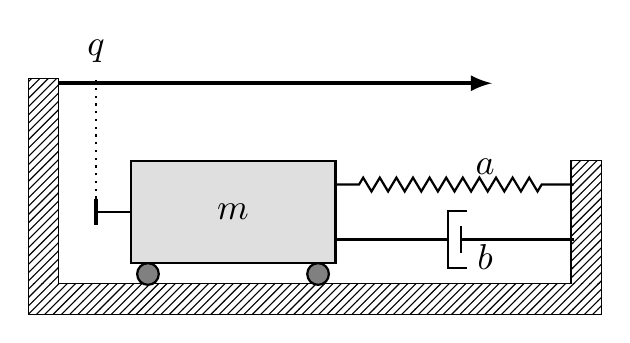
\begin{tikzpicture}[scale=1.1, every node/.style={scale=1.3}]
\tikzstyle{spring}=[thick,decorate,decoration={zigzag,pre length=0.3cm,post length=0.3cm,segment length=6}]
\tikzstyle{damper}=[thick,decoration={markings,  
  mark connection node=dmp,
  mark=at position 0.5 with 
  {
    \node (dmp) [thick,inner sep=0pt,transform shape,rotate=-90,minimum width=15pt,minimum height=3pt,draw=none] {};
    \draw [thick] ($(dmp.north east)+(2pt,0)$) -- (dmp.south east) -- (dmp.south west) -- ($(dmp.north west)+(2pt,0)$);
    \draw [thick] ($(dmp.north)+(0,-5pt)$) -- ($(dmp.north)+(0,5pt)$);
  }
}, decorate]
\tikzstyle{ground}=[fill,pattern=north east lines,draw=none,minimum width=0.75cm,minimum height=0.3cm,inner sep=0pt,outer sep=0pt]

\node [draw, outer sep=0pt, thick, fill = gray!25] (M) [minimum width=2cm, minimum height=1cm] {$m$};

\node (ground) [ground,anchor=north,yshift=-0.2cm,minimum width=5cm,xshift=0.8cm] at (M.south) {};
\draw (ground.north west) -- (ground.north east);
\draw (ground.south east) -- (ground.south west);

\node (fill) [ground,xshift=-0.15cm,minimum height = 0.3cm, minimum width = 0.3cm] at (ground.west) {};
\draw (fill.north west) -- (fill.south west) -- (fill.south east);

\draw [thick, fill = gray] (M.south west) ++(0.2cm,-0.125cm) circle (0.125cm)  (M.south east) ++(-0.2cm,-0.125cm) circle (0.125cm);

\node (wall) [ground, rotate=-90, minimum width=2cm,anchor=south east] at (fill.north west) {};
\draw (wall.north east) -- (wall.north west) -- (wall.south west) -- (wall.south east);

\node (fill2) [ground,xshift=0.15cm,minimum height = 0.3cm, minimum width = 0.3cm] at (ground.east) {};
\draw (fill2.north east) -- (fill2.south east) -- (fill2.south west);
\node (wall2) [ground, rotate=-90, minimum width=1.2cm,anchor=south east] at (fill2.north west) {};
\draw (wall2.north east) -- (wall2.north west) -- (wall2.south west) -- (wall2.south east);

\draw [-,thick] (M.west) -- +(-0.4cm,0) node [name = t] {};
\draw [-,ultra thick] (t.north) -- (t.south);
\draw [spring] (M.15) -- node [xshift=0.3cm,yshift=0.175cm] {$a$} ++(2.75cm,0cm);
\draw [damper] (M.345) -- node [xshift=0.3cm,yshift=-0.175cm] {$b$} ++(2.75cm,0cm);

\draw [-latex,ultra thick] (wall.north west) ++(0cm, -0.05cm) -- +(5cm,0cm);
\draw [dotted, thick] (t.north) -- node [yshift=0.85cm] (y1) {$q$} +(0cm,1.4cm);

\end{tikzpicture} 

        \caption[Mass--spring--damper system.]{Mass--spring--damper system. $q$ indicates the absolute position of the mass, $k$ is the stiffness of the spring and $b$ is the damping coefficient of the dashpot. $u$ is an external forcing term , i.e. the control input.}
        \label{fig:msd}
    \end{figure}
    %
    Indeed, the model is included in the class of systems treated in Example \ref{ex:ndof} and, thus, admits a port--Hamiltonian representation in the form (\ref{eq:nDOF}):
    %
    \begin{equation}\label{eq:msd}
        %
	    \left\{
	        \begin{matrix*}[l]
	        %
	        \begin{bmatrix}	\dot{q}\\\dot{p}\end{bmatrix} 
        	=
	        %
	        \begin{bmatrix}0&1\\-1&-b\end{bmatrix}
	        %
	        \begin{bmatrix}{\nabla}_{q}\Ha\\{\nabla}_{p}\Ha\end{bmatrix}
	        +
	        \begin{bmatrix}0\\1\end{bmatrix}u\\
	        %
	        y = \dot{q}
	    \end{matrix*}
	    \right.
	    %
    \end{equation}
    %
    having $\Ha$ the following expression
    %
    \begin{equation}
        \Ha(q,p) \triangleq \frac{1}{2}\left(\frac{1}{m}p^2 + kq^2\right)
    \end{equation}
    %
    The natural dissipation of the system results to be
    %
    \begin{equation}
        d(t) = \frac{b}{m}p^2(t)
    \end{equation}
    %
    which means that, if no external inputs are applied (u = 0), the energy dissipated in a time interval $\Delta t$ is
    %
    \begin{equation}
        \Ha(t+\Delta t) - \Ha(t) = -\int_t^{t+\Delta t}d(s)ds = -\frac{b}{m}\int_t^{t+\Delta t}p^2(s)ds
    \end{equation}
    %
    A numerical simulation of the autonomous system ($u = 0$) has been performed with $m = 1\text{Kg}$, $k = 1\text{N}\cdot\text{m}^{-1}$, $[q_0,p_0] = [-0.9,0]$ and increasing values of $b$ ($b = \{0, 0.5, 4\}$). The state--space trajectories are shown in Figure \ref{fig:msd_ss} while the trend of the energy function $\Ha$ and its derivative are plotted in Figure \ref{fig:msd_en}. It can be noticed that when no dissipation is present, the state moves on a closed trajectory coinciding to the level set of $\Ha$ corresponding to the initial condition. On the other hand, when $b>0$, the trajectory moves on continuously decreasing isolines of $\Ha$, converging to the minimum of $\Ha$.
    %
    \begin{figure}[!ht]
        %
        \centering
        %\definecolor{ocean}{rgb}{0.00000,0.44700,0.74100}

\begin{tikzpicture}
\begin{axis}[
width=4.7cm,
height=4.7cm,
at={(0in,0.331in)},
view={0}{90},
%colorbar,
%point meta max=1,
%point meta min=0,
%colorbar horizontal,
%colorbar style={
%	width=8cm,
	%xtick={0,0.5,...,30},
%	ylabel style={},
%	xticklabel pos=lower
%},
xmin=-1,
xmax=1,
xlabel style={at = {(0.5,-0.1)}},
xlabel={$q(t)~[\text{m}]$},
colormap = {whiteblack}{color(0cm)  = (white);color(1cm) = (black)},
ymin=-1,
ymax=1,
ylabel style={at = {(-0.1,0.5)}},
ylabel={$p(t)~~[\text{Kg}\cdot\text{m}\cdot\text{s}^{-1}]$},
title = {$b = 0$},
]
\addplot3[contour filled={number = 25,labels={false}},mesh/rows=50,mesh/cols=50,mesh/check=false,forget plot
] table {H_msd.dat};
%
\addplot [color=ocean, line width=1.5pt]
  table[row sep=crcr]{%
-0.9	0\\
-0.899985978762116	0.00502374677611179\\
-0.899943915485272	0.0100473370197254\\
-0.899873811480036	0.0150706142030572\\
-0.899775668930779	0.0200934218119792\\
-0.898864515979383	0.045194945160371\\
-0.897253229220759	0.0702612624709651\\
-0.894943062948057	0.0952728455461604\\
-0.891935817148034	0.12021022098562\\
-0.866556167581894	0.243100890831152\\
-0.82433478265803	0.361258140219576\\
-0.766080802702624	0.472373151991\\
-0.692934879863237	0.574310243919449\\
-0.57159574469494	0.69525646536542\\
-0.429575938759916	0.790997111226671\\
-0.271982982658809	0.857976109244477\\
-0.104520778155736	0.89388601006985\\
0.0850288282386656	0.896064210354996\\
0.270760502842743	0.85851276785888\\
0.444387918789485	0.782734654185993\\
0.598341317654668	0.672236675929965\\
0.717729098288624	0.543056772023867\\
0.809686351627708	0.393166992301164\\
0.870598406479674	0.228250296691519\\
0.898274320830471	0.0545970347600224\\
0.889811897020796	-0.135352450426609\\
0.841656121960294	-0.319215226608868\\
0.755793507474165	-0.488727784624207\\
0.636196599911076	-0.636466082851078\\
0.499204578160879	-0.74884379351689\\
0.342897610531003	-0.832181157591438\\
0.173296043983969	-0.883139101682734\\
-0.00304276773184864	-0.899882402642246\\
-0.193099107386494	-0.879047890570117\\
-0.374395042495857	-0.818562833492796\\
-0.538678700952401	-0.720992975113251\\
-0.678689210710439	-0.590877328023257\\
-0.78208176998692	-0.445249174982841\\
-0.854660242983259	-0.282121957692752\\
-0.89344994973405	-0.107887650551509\\
-0.897067353456202	0.0706179696186121\\
-0.861656870229052	0.259783650094596\\
-0.786868398470249	0.437024441049527\\
-0.6759572974466	0.594150635828067\\
-0.534124245467652	0.724144599357674\\
-0.37926666274982	0.816077104640675\\
-0.209258979693555	0.875317501582092\\
-0.0308847706545903	0.899369161995415\\
0.148750877550933	0.887416601629263\\
0.329911975319566	0.837250023615725\\
0.496638164711434	0.750576792150003\\
0.641566286981007	0.631043151162824\\
0.758533369018855	0.483963020253203\\
0.840135819603152	0.322367129268116\\
0.887729562045677	0.147764782921913\\
0.899259081241582	-0.0327949970736031\\
0.874406542880618	-0.212053706435706\\
0.814307468308065	-0.38290080020508\\
0.721246073776016	-0.538204058414409\\
0.598889746084512	-0.671590937717149\\
0.4522628365781	-0.777799696173517\\
0.286903249537718	-0.852853547071071\\
0.109899626394544	-0.893166776311316\\
-0.0715515382366838	-0.896965233164216\\
-0.250115685677697	-0.864243271043625\\
-0.414473342521916	-0.798637777173098\\
-0.562769104159557	-0.702162777087704\\
-0.68919018546314	-0.578464615341332\\
-0.788976298239304	-0.432380863122386\\
-0.859942410723094	-0.264757881843549\\
-0.895710441694386	-0.0863410478400795\\
-0.894682197059624	0.0955773325802905\\
-0.857049226126575	0.273611939666313\\
-0.788210264600048	0.433873762211704\\
-0.689772455903816	0.577803173444043\\
-0.565359030437231	0.699918016664419\\
-0.419689972318867	0.795751930461528\\
-0.250662182525312	0.864113283905551\\
-0.0713827461508605	0.896985836183843\\
0.110793752674927	0.892883864386328\\
0.288448687610468	0.852125632510926\\
0.446080905324193	0.781313565133823\\
0.587230384341811	0.681699302531408\\
0.706618723377257	0.556887235823636\\
0.799959754030746	0.411521580192236\\
0.866645745488919	0.24160786754609\\
0.897656855316875	0.061791545916903\\
0.891579886719193	-0.120532383537661\\
0.848815041368255	-0.297923633085357\\
0.776772068507942	-0.45385550494178\\
0.676434280384692	-0.593217366355968\\
0.551392215196233	-0.710859158496992\\
0.406240890521846	-0.80260781473624\\
0.235763920672479	-0.868211186542628\\
0.0556100101817242	-0.898020220507468\\
-0.126799660452293	-0.890668663442599\\
-0.30401079333237	-0.846609824415888\\
-0.458839274459776	-0.77378865338616\\
-0.597045479198069	-0.67299860055399\\
-0.713561193199	-0.547820501013337\\
-0.804285304910703	-0.402817342459813\\
-0.869187112300746	-0.231981107680539\\
-0.898217898452297	-0.0516141930128982\\
-0.890041852965363	0.130845313550839\\
-0.845146736011128	0.307934108054784\\
-0.771829629311282	0.462044791284077\\
-0.670754142275347	0.599501243694139\\
-0.545494480244833	0.715287843149394\\
-0.400592745570706	0.805349640824099\\
-0.229527499511341	0.869795860164889\\
-0.0490265282014425	0.898321962731183\\
0.133461207998266	0.889611903861583\\
0.310466664222015	0.844175798061154\\
0.464109235032052	0.770541254692729\\
0.601077809882663	0.669284812780502\\
0.716390736941523	0.543976201673356\\
0.806022850199626	0.399143881337367\\
0.870172626986749	0.227933304279566\\
0.898371032325233	0.0473487401235774\\
0.889314867851617	-0.135153904372446\\
0.843528752436341	-0.31210197061193\\
0.769690696967145	-0.465438306186725\\
0.668319537299387	-0.602088379099282\\
0.542981991550036	-0.717092567144113\\
0.398197585001911	-0.806445000685628\\
0.226895642961435	-0.870401440052721\\
0.0462599225123437	-0.89838680870328\\
-0.136249275749539	-0.88910626668762\\
-0.313157063808946	-0.843093841429669\\
-0.466292179948039	-0.769125422475537\\
-0.602733461364698	-0.667681882722236\\
-0.717535624244837	-0.542327907989\\
-0.806705347801197	-0.397577148152829\\
-0.870535302904268	-0.226218728793038\\
-0.898381979336706	-0.0455527758883808\\
-0.888955983468011	0.136957675044427\\
-0.842797442857704	0.313836406768774\\
-0.768745811759756	0.466838455208328\\
-0.667257100626571	0.603142072049961\\
-0.541894610327008	0.717811343580643\\
-0.3971681029494	0.806861142132291\\
-0.225775795247881	0.870607982511503\\
-0.0450931383464444	0.898364195615979\\
0.13741517512899	0.888843944052419\\
0.314272183805362	0.842591307422162\\
0.467185401798536	0.768486935302289\\
0.60339749240315	0.666970601259239\\
0.717978696770325	0.541604646474109\\
0.806949262779914	0.396896236368967\\
0.870641132546805	0.225484680727458\\
0.898338179640358	0.0447940797609513\\
0.888756895967326	-0.137709916911727\\
0.842443918418608	-0.314549983926374\\
0.768306529621424	-0.467403089395834\\
0.666773917190017	-0.603553593140095\\
0.541407740824552	-0.718075807977677\\
0.396713407860014	-0.806993532318025\\
0.225292099096355	-0.870648698993944\\
0.044599231719254	-0.898306894149129\\
-0.137899042369989	-0.888686142455428\\
-0.314725280748879	-0.842334732474257\\
-0.467536918222569	-0.768177108575129\\
-0.603645267281041	-0.666635562821397\\
-0.718127361651747	-0.541271254952529\\
-0.807009367141457	-0.396588378820279\\
-0.870639689216012	-0.2251634771752\\
-0.898272219395117	-0.0444720255551413\\
-0.888625997969875	0.138019617151321\\
-0.842250377147011	0.314834051838949\\
-0.768080806524671	0.467616326505174\\
-0.666535087765261	0.603695135187654\\
-0.541173998881901	0.718149356250842\\
-0.396500873907206	0.807006755463903\\
-0.225076377178532	0.870619931626889\\
-0.0443887302599181	0.898235357938574\\
0.138095692727857	0.888572754542549\\
0.314899640143905	0.842182155481042\\
0.467660411717213	0.768006015271765\\
0.603717869337494	0.666459210631732\\
0.71815216736394	0.541102214776562\\
0.806992173553473	0.396437731579442\\
0.870593202186712	0.225016234617949\\
0.898197082902773	0.0443339426802373\\
0.888523997689305	-0.138142879393263\\
0.84212441451158	-0.314937195052407\\
0.767945194178618	-0.467681566861691\\
0.666399306516848	-0.603722990341367\\
0.541046969963166	-0.718142526757086\\
0.396390407362998	-0.806969822650201\\
0.224973594555328	-0.87056194908907\\
0.044297663761356	-0.898157893035261\\
-0.138171310304688	-0.888478156768335\\
-0.31495655009187	-0.842073481204946\\
-0.467687835818486	-0.767893445632694\\
-0.603716677343032	-0.666349774690757\\
-0.718124803240385	-0.541002464545261\\
-0.806942429033045	-0.396353353853221\\
-0.870527760464342	-0.224942318616057\\
-0.898118110808496	-0.0442734020123234\\
-0.888434210726434	0.13818756386025\\
-0.842026969566038	0.3149640889562\\
-0.767847588973596	0.467684440287652\\
-0.666306978334444	0.603702941392205\\
-0.540964932665922	0.718101832602381\\
-0.396322969320124	0.806911762216299\\
-0.224918421433181	0.870491666866797\\
-0.0442569428617527	0.898077945029905\\
0.138195910990712	0.888391496069198\\
0.314963956088771	0.841983329898185\\
0.392640782142731	0.8086860382096\\
0.466846309430426	0.76824222783696\\
0.536922826942551	0.721008736510139\\
0.602254599556311	0.667402836362263\\
}
[postaction={decorate, decoration={markings,
		mark=between positions 0.4 and 1 step 1 with {\arrow[black,line width=1.5pt]{latex};}
}}]
;
\addplot [color=black, line width=1.0pt, draw=none, mark=*, mark options={solid, fill=red}]
table[row sep=crcr]{%
	0	0\\
};
\end{axis}
%
%
%%%%%%%%%%%%%%%%%%%%%%%%%%%%%%%%%%%%%%%%%%%%%%%%%%%%%%%%%%%%%%%%%%%%%%%%%%%%%%%%%%%%
%%%%%%%%%%%%%%%%%%%%%%%%%%%%%%%%%%%%%%%%%%%%%%%%%%%%%%%%%%%%%%%%%%%%%%%%%%%%%%%%%%%%
%%%%%%%%%%%%%%%%%%%%%%%%%%%%%%%%%%%%%%%%%%%%%%%%%%%%%%%%%%%%%%%%%%%%%%%%%%%%%%%%%%%%
%%%%%%%%%%%%%%%%%%%%%%%%%%%%%%%%%%%%%%%%%%%%%%%%%%%%%%%%%%%%%%%%%%%%%%%%%%%%%%%%%%%%
%%%%%%%%%%%%%%%%%%%%%%%%%%%%%%%%%%%%%%%%%%%%%%%%%%%%%%%%%%%%%%%%%%%%%%%%%%%%%%%%%%%%
%%%%%%%%%%%%%%%%%%%%%%%%%%%%%%%%%%%%%%%%%%%%%%%%%%%%%%%%%%%%%%%%%%%%%%%%%%%%%%%%%%%%
%%%%%%%%%%%%%%%%%%%%%%%%%%%%%%%%%%%%%%%%%%%%%%%%%%%%%%%%%%%%%%%%%%%%%%%%%%%%%%%%%%%%
%%%%%%%%%%%%%%%%%%%%%%%%%%%%%%%%%%%%%%%%%%%%%%%%%%%%%%%%%%%%%%%%%%%%%%%%%%%%%%%%%%%%
%%%%%%%%%%%%%%%%%%%%%%%%%%%%%%%%%%%%%%%%%%%%%%%%%%%%%%%%%%%%%%%%%%%%%%%%%%%%%%%%%%%%
%%%%%%%%%%%%%%%%%%%%%%%%%%%%%%%%%%%%%%%%%%%%%%%%%%%%%%%%%%%%%%%%%%%%%%%%%%%%%%%%%%%%
%
%
\begin{axis}[
width=4.7cm,
height=4.7cm,
at={(1.6in,0.331in)},
view={0}{90},
colormap = {whiteblack}{color(0cm)  = (white);color(1cm) = (black)},
xmin=-1,
xmax=1,
xlabel style={at = {(0.5,-0.1)}},
xlabel={$q(t)~[\text{m}]$},
ymin=-1,
ymax=1,
ylabel style={at = {(-0.1,0.5)}},
ylabel={$p(t)~~[\text{Kg}\cdot\text{m}\cdot\text{s}^{-1}]$},
title = {$b = 0.5$},
]
\addplot3[contour filled={number = 25,labels={false}},mesh/rows=50,mesh/cols=50,mesh/check=false,forget plot
] table {H_msd.dat};
%
\addplot [color=ocean, line width=1.5pt]
table[row sep=crcr]{%
	-0.9	0\\
	-0.899985991795746	0.00501674269174762\\
	-0.899944019691303	0.0100193471557007\\
	-0.899874162931692	0.0150076971406221\\
	-0.89977650140532	0.0199816771641279\\
	-0.898873958295022	0.0446320420072224\\
	-0.897288646861763	0.0689062780415569\\
	-0.8950312582937	0.0927908195727069\\
	-0.892112845290034	0.116272595485913\\
	-0.868002952216995	0.227228035383425\\
	-0.829223766085857	0.326435243373571\\
	-0.777500187200184	0.412807338237014\\
	-0.714659008971771	0.485603292982159\\
	-0.600340602727355	0.570331414933827\\
	-0.471488130080395	0.621495133714803\\
	-0.335347897263502	0.640176352681101\\
	-0.198445114013884	0.628945422916099\\
	-0.0746437735806325	0.594456994280607\\
	0.0401381420897199	0.540383416283467\\
	0.142232199262124	0.470719359197013\\
	0.229035654600393	0.389586456149254\\
	0.290490142676407	0.313265041426897\\
	0.338339729122556	0.23421079930552\\
	0.372303052526759	0.154991891744638\\
	0.392571550535566	0.0778835525828194\\
	0.399731808807902	-0.00306277450207788\\
	0.391870981971099	-0.0763851640723532\\
	0.370660517667212	-0.14009523114136\\
	0.338087981923116	-0.192856605316552\\
	0.298136191440485	-0.232477962681855\\
	0.25184670416552	-0.260834031598041\\
	0.201350587767438	-0.277964416164619\\
	0.148664452554781	-0.284317405805023\\
	0.0907667653016975	-0.27983068280962\\
	0.0349146831770288	-0.264713991318473\\
	-0.0168257578844223	-0.240602883573134\\
	-0.0628664499768871	-0.20930778888674\\
	-0.0980374609679892	-0.17699717235111\\
	-0.127063690395628	-0.141926700215142\\
	-0.149546840710965	-0.105459101422993\\
	-0.165363769927057	-0.0688391130058303\\
	-0.17517242929207	-0.0298002370528735\\
	-0.177436179549933	0.00664995096132089\\
	-0.172778407588365	0.0393477927721653\\
	-0.162032775025325	0.0674497666527798\\
	-0.147454933577949	0.0889207675276733\\
	-0.129347064906398	0.10558047092737\\
	-0.108623814628922	0.117297644237556\\
	-0.086179982857339	0.124136300367046\\
	-0.0599942658276899	0.126273096752299\\
	-0.03394383333752	0.123024483749271\\
	-0.00911017489546286	0.115053707894857\\
	0.0136390018342169	0.103150490035125\\
	0.0323115311721372	0.0893174145892377\\
	0.0481096403624088	0.0735852869681779\\
	0.0607228554124504	0.0566997231192924\\
	0.0700087283561835	0.0393538111534125\\
	0.0761616883827873	0.0213703319404493\\
	0.0787495703594155	0.00429179247670834\\
	0.0780099609822195	-0.0112862674191978\\
	0.0742949609073913	-0.0249184536659205\\
	0.0676235361779361	-0.0368399446136417\\
	0.0587030242407405	-0.0459531423309749\\
	0.0481558122411435	-0.0521341873494105\\
	0.0365928902454288	-0.0554253293582465\\
	0.0240750228983752	-0.0559548535184\\
	0.0117514398745198	-0.0537959330321324\\
	0.00019941613886286	-0.0493329003279672\\
	-0.0101378207178845	-0.0430176266200058\\
	-0.019073150754024	-0.0351836299097121\\
	-0.0261146445062195	-0.0264793026690255\\
	-0.0311080878005064	-0.0174345850654783\\
	-0.0340432057031742	-0.00851368245135384\\
	-0.0350111008169466	0.000208271867982888\\
	-0.034025886560588	0.00794187081482636\\
	-0.0313546321013023	0.014373201383412\\
	-0.0273270827992865	0.0193247845816726\\
	-0.021776682313328	0.0229649845032737\\
	-0.0155344254822122	0.0247149856554559\\
	-0.00909170615632734	0.0246816915211178\\
	-0.00286371969873624	0.0230947709063524\\
	0.00280725028199055	0.0202496734322155\\
	0.00760795718689828	0.016477401614915\\
	0.0113249300742123	0.0121348606754593\\
	0.0138716616756584	0.00755763965809117\\
	0.0153115070918749	0.00268446415992479\\
	0.0154380718037925	-0.00174353700984352\\
	0.0144046855261442	-0.0054393994641403\\
	0.0124469315254243	-0.00824628912471304\\
	0.00973633834811147	-0.0101436953203082\\
	0.00663307131848225	-0.0109904365212177\\
	0.00344345203354436	-0.010849788231025\\
	0.000418598885933671	-0.00987679726686231\\
	-0.00236889674029977	-0.00817147420768934\\
	-0.00455610701932897	-0.00600636910422985\\
	-0.0060212570956228	-0.00363960519553869\\
	-0.00675662344583174	-0.00129708301418448\\
	-0.00679915540873005	0.000997090639439771\\
	-0.00615806076904666	0.0028415988465903\\
	-0.00499448977320246	0.00409954744618751\\
	-0.00350966028254127	0.0047525483255705\\
	-0.00178742736195878	0.00483753431425414\\
	-0.000142544164199142	0.00436296059647222\\
	0.001233863384226	0.00346409628606365\\
	0.00224352413019931	0.0023187867470898\\
	0.00286423019005585	0.001064908755426\\
	0.00304301781878184	-0.000107287213496858\\
	0.00281783500493549	-0.0010575880234264\\
	0.0022937627777237	-0.00172125518888289\\
	0.00153324548129663	-0.00210115118921709\\
	0.000699028537681449	-0.00212944532957787\\
	-7.39090484163769e-05	-0.00185022451593175\\
	-0.000696860580362937	-0.0013673867011887\\
	-0.00115698870029392	-0.000733929244931739\\
	-0.00134549775988726	-0.000103223462323883\\
	-0.00126431291907824	0.000412349861050412\\
	-0.000993032124110712	0.000759026310963054\\
	-0.000596744297566764	0.000936587972301828\\
	-0.0001714552068425	0.000909680277066964\\
	0.000192405808728558	0.000708505171052146\\
	0.000443835290730197	0.000417655115078066\\
	0.000582041712668234	8.20914139281743e-05\\
	0.000563673850896241	-0.000200244790181628\\
	0.000407680747611572	-0.000363593139831435\\
	0.000193602312173417	-0.000405181279185971\\
	-2.30281468151146e-05	-0.000352938747129361\\
	-0.000186564607289939	-0.000224639431191565\\
	-0.000253723590669539	-6.14216529346211e-05\\
	-0.000236476036563678	7.85096220374468e-05\\
	-0.000162705457701936	0.000174617140937539\\
	-5.64067851445571e-05	0.000196804176492543\\
	4.62570015027289e-05	0.000136732345109551\\
	0.000106953605066236	4.5051528543188e-05\\
	0.00012515523979931	-5.30186446630676e-05\\
	8.69067523052607e-05	-0.000109998447934223\\
	-2.80092519366811e-06	-9.06136603478964e-05\\
	-7.20860461539662e-05	-2.64132971781262e-05\\
	-7.64796094496801e-05	2.09540211186838e-05\\
	-5.84460433855426e-05	5.1911771294405e-05\\
	-2.42154646050572e-05	5.68361010025379e-05\\
	8.96341400149207e-06	4.27250166876023e-05\\
}
[postaction={decorate, decoration={markings,
		mark=between positions 0.4 and 1 step 1 with {\arrow[black,line width=1.5pt]{latex};}
}}]
;
\addplot [color=black, line width=1.0pt, draw=none, mark=*, mark options={solid, fill=red}]
table[row sep=crcr]{%
	0	0\\
};
\end{axis}
%
%
%
%%%%%%%%%%%%%%%%%%%%%%%%%%%%%%%%%%%%%%%%%%%%%%%%%%%%%%%%%%%%%%%%%%%%%%%%%%%%%%%%%%%%
%%%%%%%%%%%%%%%%%%%%%%%%%%%%%%%%%%%%%%%%%%%%%%%%%%%%%%%%%%%%%%%%%%%%%%%%%%%%%%%%%%%%
%%%%%%%%%%%%%%%%%%%%%%%%%%%%%%%%%%%%%%%%%%%%%%%%%%%%%%%%%%%%%%%%%%%%%%%%%%%%%%%%%%%%
%%%%%%%%%%%%%%%%%%%%%%%%%%%%%%%%%%%%%%%%%%%%%%%%%%%%%%%%%%%%%%%%%%%%%%%%%%%%%%%%%%%%
%%%%%%%%%%%%%%%%%%%%%%%%%%%%%%%%%%%%%%%%%%%%%%%%%%%%%%%%%%%%%%%%%%%%%%%%%%%%%%%%%%%%
%%%%%%%%%%%%%%%%%%%%%%%%%%%%%%%%%%%%%%%%%%%%%%%%%%%%%%%%%%%%%%%%%%%%%%%%%%%%%%%%%%%%
%%%%%%%%%%%%%%%%%%%%%%%%%%%%%%%%%%%%%%%%%%%%%%%%%%%%%%%%%%%%%%%%%%%%%%%%%%%%%%%%%%%%
%%%%%%%%%%%%%%%%%%%%%%%%%%%%%%%%%%%%%%%%%%%%%%%%%%%%%%%%%%%%%%%%%%%%%%%%%%%%%%%%%%%%
%%%%%%%%%%%%%%%%%%%%%%%%%%%%%%%%%%%%%%%%%%%%%%%%%%%%%%%%%%%%%%%%%%%%%%%%%%%%%%%%%%%%
%%%%%%%%%%%%%%%%%%%%%%%%%%%%%%%%%%%%%%%%%%%%%%%%%%%%%%%%%%%%%%%%%%%%%%%%%%%%%%%%%%%%
%
%
\begin{axis}[
width=4.7cm,
height=4.7cm,
at={(3.2in,0.331in)},
view={0}{90},
colorbar,
colorbar style={at = {(1.1,1)}},
colormap = {whiteblack}{color(0cm)  = (white);color(1cm) = (black)},
xmin=-1,
xmax=1,
xlabel style={at = {(0.5,-0.1)}},
xlabel={$q(t)~[\text{m}]$},
ymin=-1,
ymax=1,
ylabel style={at = {(-0.1,0.5)}},
ylabel={$p(t)~~[\text{Kg}\cdot\text{m}\cdot\text{s}^{-1}]$},
title = {$b = 4$},
]
\addplot3[contour filled={number = 25,labels={false}},mesh/rows=50,mesh/cols=50,mesh/check=false,forget plot
] table {H_msd.dat};
%
\addplot [color=ocean, line width=1.5pt]
  table[row sep=crcr]{%
-0.9	0\\
-0.899986082645966	0.00496807747392556\\
-0.899944741235495	0.00982630422634904\\
-0.899876582497193	0.0145769558126085\\
-0.899782200827883	0.0192222617484558\\
-0.898937295834081	0.0409449346364979\\
-0.897518958868064	0.0603421916601764\\
-0.895588421556982	0.0776439332126916\\
-0.893201763376469	0.0930608213725001\\
-0.888467630367654	0.114636134376241\\
-0.88284013574678	0.13240211607597\\
-0.876474556988541	0.146944025341799\\
-0.86951051919345	0.15878863662014\\
-0.860767020484186	0.169814482142593\\
-0.851505837159158	0.178290748528594\\
-0.841844848322571	0.184666101724681\\
-0.831890964066219	0.189348148743069\\
-0.819922923413661	0.193144938047076\\
-0.807765054855702	0.195427678175533\\
-0.795495822471476	0.196502591719694\\
-0.783188641803364	0.196656840595652\\
-0.768828558561473	0.195977393204228\\
-0.754545230339636	0.194557417626953\\
-0.74037988509665	0.192570708874763\\
-0.726374152465561	0.19019218106681\\
-0.709930503100259	0.18703317551019\\
-0.693773915607893	0.183601271819889\\
-0.677918254874043	0.179979251204216\\
-0.662381915451248	0.176266098599558\\
-0.643909528408537	0.171727073309734\\
-0.625919133286568	0.16718029232227\\
-0.608404370337005	0.162652685113731\\
-0.591365866648016	0.15819587379239\\
-0.57069763875581	0.152769095348656\\
-0.550740870625205	0.147487724855014\\
-0.531471415233416	0.142349448081369\\
-0.512873108408636	0.137378779337122\\
-0.489667953616186	0.131190380410974\\
-0.467509128297243	0.125267241437474\\
-0.446347742199929	0.119591502705154\\
-0.426144152762347	0.114172734423179\\
-0.400629926416631	0.107355847295774\\
-0.376640389229073	0.100934881526313\\
-0.354080496864401	0.0948716574943904\\
-0.332873177659729	0.0891774784751443\\
-0.309192802097066	0.0828914215528698\\
-0.287187463749281	0.0770122627642054\\
-0.266721849886632	0.0714500052344186\\
-0.247721578882146	0.0663152319700499\\
-0.235332380989259	0.0630473273196916\\
-0.223555882782269	0.0599145511485628\\
-0.212356300818894	0.0568909693815244\\
-0.201718716473235	0.0540234317934798\\
-0.191624945138423	0.0513414642642776\\
-0.182033235044434	0.0487813166094927\\
-0.172916226635376	0.0463285063332356\\
-0.164256241958628	0.0440005428570637\\
-0.154192940274117	0.0413250355594885\\
-0.144742987935158	0.0388002037388014\\
-0.135864440383816	0.0364003659516473\\
-0.127532027626431	0.0341546455949839\\
-0.11867525331641	0.0318397432202277\\
-0.110424117802772	0.0296462452233622\\
-0.102720927337247	0.0275072921528232\\
-0.0955615479928512	0.0255465046723676\\
-0.0907381036725926	0.0243054153897836\\
-0.0861511905380074	0.0230986312563235\\
-0.0817834618112206	0.0219043159164131\\
-0.0776382192477248	0.0207756466920797\\
-0.0737145894339448	0.0197481502155475\\
-0.0699860348159163	0.0187594277043537\\
-0.0664401907463775	0.0177981869562598\\
-0.0630744837884715	0.016888013555112\\
-0.0592354982555055	0.0158814525643452\\
-0.0556267970963887	0.0149222285045181\\
-0.0522297787311866	0.0139903414637984\\
-0.0490417813313194	0.0131224888356137\\
-0.045694345896388	0.0122818281174344\\
-0.0425662959639533	0.0114607578362246\\
-0.0396278134669222	0.01060267571815\\
-0.0368981598790105	0.00983072429130796\\
-0.0346176475321157	0.00932980917812475\\
-0.0324609504412467	0.00878920287401631\\
-0.0303959030482267	0.00812023534849494\\
-0.0284709357107608	0.00753321001535077\\
-0.027036814674421	0.00723476502613525\\
-0.0256632203417544	0.00690348866292727\\
-0.0243375487692109	0.0065055721629652\\
-0.0230823335715312	0.00613770393489952\\
-0.0219897582296346	0.0058798220601638\\
-0.0209444049957792	0.0056158135687297\\
-0.0199413667985639	0.0053360632175165\\
-0.0189866393141357	0.00507125204892422\\
-0.0179406546491316	0.00480993378101063\\
-0.0169495594311861	0.00455179936258552\\
-0.0160073979751741	0.00428577216967137\\
-0.0151184277995411	0.00403831426009074\\
-0.0141217823491402	0.00380468280381971\\
-0.0131854939453885	0.00356432451439736\\
-0.0122971854676326	0.00328645139318065\\
-0.0114719702953549	0.00304193200650151\\
-0.0107223959060257	0.00293256752726012\\
-0.0100070221485357	0.00276914912020248\\
-0.00930002128788741	0.00246753902563632\\
-0.00865221342488059	0.00222889577297575\\
-0.00819570426968582	0.00221813736602114\\
-0.00774688741497106	0.00214074235362552\\
-0.00728706051438759	0.00193227456454014\\
-0.0068598192928206	0.00176051537180819\\
-0.00654856550325697	0.0017340497738052\\
-0.00624408447372882	0.00167881023150739\\
-0.00594178964708822	0.00158025065149906\\
-0.00565454541941408	0.00148883680750362\\
-0.00537631531292838	0.00143666730759179\\
-0.00510876224949485	0.00137475777312649\\
-0.00484908050613714	0.00129512771363616\\
-0.00460302015824542	0.00122160917506098\\
-0.0043257230973134	0.00116857898401966\\
-0.00406184985623664	0.00110522950674168\\
-0.00380605501587365	0.00101532240997032\\
-0.00356793433038374	0.000938169297570303\\
-0.00333665932120208	0.000935530160271736\\
-0.00311064338403006	0.000892692236794176\\
-0.00287359615302805	0.000753008166497469\\
-0.00266101927641805	0.00065285826477333\\
-0.00254075383157781	0.000672470837606742\\
-0.00241886203059497	0.000662361458281949\\
-0.00229005848898741	0.000603997717300565\\
-0.00216912478822883	0.000553681341221306\\
-0.00206605484478845	0.000549788868306814\\
-0.00196466545728071	0.000532943003154328\\
-0.00186241530959827	0.000494629061489078\\
-0.00176595315861278	0.0004605840091987\\
-0.00166440462563356	0.000455192922624221\\
-0.00156533360834748	0.000436278444277397\\
-0.00146406235327491	0.000387768271416189\\
-0.00137087292765273	0.000349342709335403\\
-0.00129252077162399	0.000384511033847523\\
-0.00120936534690071	0.000379239845324055\\
-0.00110691404776746	0.000280985547766188\\
-0.00101883911082306	0.000216861400234995\\
-0.000985990722304886	0.000319325363220362\\
-0.000935945018704741	0.000343480939004773\\
-0.000844991771327944	0.000201725450129464\\
-0.000770667066740696	0.000109620309690839\\
-0.000754885535685853	0.000192279139905914\\
-0.000726866332776939	0.000222023119262845\\
-0.000677630930385176	0.000165714133679594\\
-0.000633528122700672	0.000122039584436439\\
-0.000612817141307044	0.000151517158153205\\
-0.000588141102822837	0.000161112680779031\\
-0.000557064186939311	0.000141977419568236\\
-0.000527871879127115	0.000125264189015855\\
-0.000503867370637172	0.000137633130787744\\
-0.000478193924392654	0.000138138588242503\\
-0.000448065129271954	0.00011669254140118\\
-0.000420611381925702	0.00010020091846496\\
-0.000401922160366452	0.000128294451075975\\
}
[postaction={decorate, decoration={markings,
		mark=between positions 0.6 and 1 step 1 with {\arrow[black,line width=1.5pt]{latex};}
}}]
;
\addplot [color=black, line width=1.0pt, draw=none, mark=*, mark options={solid, fill=red}]
table[row sep=crcr]{%
	0	0\\
};
\end{axis}

\end{tikzpicture}
        %
        \caption[State--space trajectory of the mass--spring damper system for different values of the damping coefficient.]{State--space trajectory of the mass--spring damper system for different values of the damping coefficient. The background is the filled contour of the energy function $\Ha$. When $b = 0$, the is no energy dissipation and motion happen on a periodic trajectory (closed curve), i.e. the level set of $\Ha$ corresponding to the initial conditions. When $b = 0.5, 4$, the state converges toward the minimum of the energy with or without oscillations. The convergence happens by converting elastic potential energy into kinetic energy which is partially dissipated by the dashpot before being reconverted to elastic potential. Higher values of the damping coefficient implies grater dissipation.}
        \label{fig:msd_ss}
    \end{figure}
    %
    \begin{figure}[!ht]
        %
        \centering
        %%
\definecolor{ocean}{rgb}{0.00000,0.44700,0.74100}
%
\begin{tikzpicture}

\begin{axis}[%
width=0.75\linewidth,
height=1.5cm,
at={(1.124in,10cm)},
scale only axis,
xmin=0,
xmax=12,
ymin=-0.205,
ymax=0.405,
%title={$b = 0$},
legend style={legend cell align=left, align=left, draw=white!15!black}
]
\node[draw] at (5cm,1cm) {$b = 0$};
\addplot [color=black, line width=2.0pt]
  table[row sep=crcr]{%
0	0.405\\
0.00558196984779907	0.405000000000037\\
0.0111639396955981	0.405000000000075\\
0.0167459095433972	0.405000000000033\\
0.0223278793911963	0.404999999999972\\
0.0502377286301916	0.405000000577449\\
0.0781475778691869	0.405000001175547\\
0.106057427108182	0.405000000508656\\
0.133967276347178	0.404999999570472\\
0.273489076266092	0.405008817348559\\
0.413010876185006	0.405017638887384\\
0.55253267610392	0.405008095495705\\
0.692054476022834	0.404995502000948\\
0.882622882851168	0.40505162399289\\
1.0731912896795	0.405105958565201\\
1.26375969650783	0.405048873445136\\
1.45432810333617	0.404978396032439\\
1.66522448061415	0.405080485355381\\
1.87612085789213	0.405177711238185\\
2.08701723517011	0.405077080614858\\
2.29791361244809	0.404957240439046\\
2.49359204877776	0.405022858085592\\
2.68927048510742	0.405086135923666\\
2.88494892143709	0.405019891652357\\
3.08062735776676	0.404938795834016\\
3.29217572928616	0.405042748958118\\
3.50372410080557	0.405141694266096\\
3.71527247232497	0.405039336701893\\
3.92682084384437	0.404917594179105\\
4.12394370956561	0.404986118972774\\
4.32106657528686	0.405052125179049\\
4.5181894410081	0.40498309589074\\
4.71531230672934	0.404898798510326\\
4.92804917914053	0.405006229594616\\
5.14078605155172	0.405108380110615\\
5.35352292396291	0.405002806511212\\
5.5662597963741	0.404877530753331\\
5.76496475773265	0.404949361384387\\
5.96366971909119	0.405018464974297\\
6.16237468044974	0.404946278910651\\
6.36107964180828	0.404858367134985\\
6.57522767025033	0.404970053434698\\
6.78937569869237	0.405076119292893\\
7.00352372713441	0.404966623013104\\
7.21767175557645	0.404837055187637\\
7.41804847500585	0.404912521096047\\
7.61842519443524	0.404985024579151\\
7.81880191386464	0.40490937930336\\
8.01917863329403	0.404817524209702\\
8.22835222657444	0.404914756751895\\
8.43752581985484	0.405007493781065\\
8.64669941313525	0.404911379610052\\
8.85587300641565	0.404796538443848\\
9.05730825802623	0.404874380706413\\
9.2587435096368	0.404949103200885\\
9.46017876124737	0.404871203514256\\
9.66161401285794	0.404776788322777\\
9.86314170214268	0.40485483786999\\
10.0646693914274	0.40492975371553\\
10.2661970807122	0.404851657794485\\
10.4677247699969	0.404757020358642\\
10.6697989726996	0.404836323673505\\
10.8718731754022	0.404912409094004\\
11.0739473781048	0.404833126064686\\
11.2760215808075	0.404737143883105\\
11.4570161856056	0.404778485302241\\
11.6380107904037	0.404818793251919\\
11.8190053952019	0.40477617483988\\
12	0.404722769265542\\
};
\addlegendentry{$\Ha(q,p)$}

\addplot [color=ocean, dotted, line width=2.0pt]
  table[row sep=crcr]{%
0	0\\
0.00558196984779907	0\\
0.0111639396955981	0\\
0.0167459095433972	0\\
0.0223278793911963	0\\
0.0502377286301916	0\\
0.0781475778691869	0\\
0.106057427108182	0\\
0.133967276347178	0\\
0.273489076266092	0\\
0.413010876185006	0\\
0.55253267610392	0\\
0.692054476022834	0\\
0.882622882851168	0\\
1.0731912896795	0\\
1.26375969650783	0\\
1.45432810333617	0\\
1.66522448061415	0\\
1.87612085789213	0\\
2.08701723517011	0\\
2.29791361244809	0\\
2.49359204877776	0\\
2.68927048510742	0\\
2.88494892143709	0\\
3.08062735776676	0\\
3.29217572928616	0\\
3.50372410080557	0\\
3.71527247232497	0\\
3.92682084384437	0\\
4.12394370956561	0\\
4.32106657528686	0\\
4.5181894410081	0\\
4.71531230672934	0\\
4.92804917914053	0\\
5.14078605155172	0\\
5.35352292396291	0\\
5.5662597963741	0\\
5.76496475773265	0\\
5.96366971909119	0\\
6.16237468044974	0\\
6.36107964180828	0\\
6.57522767025033	0\\
6.78937569869237	0\\
7.00352372713441	0\\
7.21767175557645	0\\
7.41804847500585	0\\
7.61842519443524	0\\
7.81880191386464	0\\
8.01917863329403	0\\
8.22835222657444	0\\
8.43752581985484	0\\
8.64669941313525	0\\
8.85587300641565	0\\
9.05730825802623	0\\
9.2587435096368	0\\
9.46017876124737	0\\
9.66161401285794	0\\
9.86314170214268	0\\
10.0646693914274	0\\
10.2661970807122	0\\
10.4677247699969	0\\
10.6697989726996	0\\
10.8718731754022	0\\
11.0739473781048	0\\
11.2760215808075	0\\
11.4570161856056	0\\
11.6380107904037	0\\
11.8190053952019	0\\
12	0\\
};
\addlegendentry{$\dot{\Ha}(q,p)$}

\end{axis}

\begin{axis}[%
width=0.75\linewidth,
height=1.5cm,
at={(1.124in,8cm)},
scale only axis,
xmin=0,
xmax=12,
ymin=-0.205,
ymax=0.405,
ylabel={$\Ha(q,p)~~\left[\text{J}\right],~~~\dot{\Ha}(q,p)~~\left[\text{W}\right]$},
legend style={legend cell align=left, align=left, draw=white!15!black}
]
\node[draw] at (5cm,1cm) {$b = 0.5$};
\addplot [color=black, line width=2.0pt]
  table[row sep=crcr]{%
0	0.405\\
0.00558196984779907	0.404999976567903\\
0.0111639396955981	0.404999812947783\\
0.0167459095433972	0.404999370042739\\
0.0223278793911963	0.404998509951744\\
0.0502377286301916	0.404983206037347\\
0.0781475778691869	0.404937495470277\\
0.106057427108182	0.404845544759889\\
0.133967276347178	0.404692322596255\\
0.273516522542154	0.402530852560815\\
0.413065768737131	0.397086011178988\\
0.552615014932108	0.387458219799325\\
0.692164261127084	0.373274028629815\\
0.907269193523539	0.342843381071733\\
1.12237412591999	0.304278629018944\\
1.33747905831645	0.261141987365565\\
1.5525839907129	0.217476404141547\\
1.75422600025637	0.179475405491745\\
1.95586800979984	0.146812653522303\\
2.1575100193433	0.120903356814893\\
2.35915202888677	0.102117468946583\\
2.53381146818428	0.0912597545861774\\
2.70847090748178	0.0846642354070274\\
2.88313034677929	0.0813160247136622\\
3.05778978607679	0.0800891350264095\\
3.25229709785627	0.0798974497802438\\
3.44680440963575	0.0796987799006767\\
3.64131172141523	0.0785079465729382\\
3.8358190331947	0.0757485768675346\\
4.0227142230037	0.0714655958896716\\
4.2096094128127	0.0657305772193612\\
4.39650460262169	0.058903137924015\\
4.58339979243069	0.0514687533485556\\
4.78779223544894	0.0432719083625159\\
4.99218467846718	0.0356462661505543\\
5.19657712148542	0.0290864268560461\\
5.40096956450367	0.0238809705106763\\
5.58272031174094	0.0204696713866693\\
5.76447105897822	0.0181441848254574\\
5.94622180621549	0.016742939819788\\
6.12797255345277	0.016041999941959\\
6.32751523007192	0.0157867170562464\\
6.52705790669108	0.015763909830532\\
6.72660058331024	0.0157003134624063\\
6.92614325992939	0.015402045601961\\
7.11151061116563	0.014824930167094\\
7.29687796240187	0.0139389495205726\\
7.48224531363811	0.0127789352241093\\
7.66761266487435	0.0114184052570543\\
7.87576626103452	0.00977210344780954\\
8.08391985719468	0.00814360371171002\\
8.29207345335485	0.0066601754934905\\
8.50022704951501	0.00541302298276011\\
8.69377185543363	0.00451081779779689\\
8.88731666135224	0.0038646659769947\\
9.08086146727086	0.00345106188562289\\
9.27440627318948	0.00322497224917417\\
9.47733620279232	0.00312864693228089\\
9.68026613239515	0.00310995715722783\\
9.88319606199799	0.00310646692235253\\
10.0861259916008	0.00307033527466572\\
10.3002873334557	0.00296506208217241\\
10.5144486753105	0.0027788681725499\\
10.7286100171654	0.00251847787159385\\
10.9427713590203	0.00220550337549205\\
11.1662986311212	0.00185527617991145\\
11.3898259032222	0.00151604937496107\\
11.6133531753232	0.00121688741078279\\
11.8368804474241	0.000976645804463098\\
11.8776603355681	0.000940047157137025\\
11.9184402237121	0.000905716717419815\\
11.959220111856	0.000873647677976041\\
12	0.000843821433264805\\
};

\addplot [color=ocean, dotted, line width=2.0pt]
  table[row sep=crcr]{%
0	0\\
0.00558196984779907	-1.25838536176011e-05\\
0.0111639396955981	-5.01936587132233e-05\\
0.0167459095433972	-0.000112615486732318\\
0.0223278793911963	-0.000199633711145713\\
0.0502377286301916	-0.000996009586867228\\
0.0781475778691869	-0.00237403757677018\\
0.106057427108182	-0.00430506809848731\\
0.133967276347178	-0.00675965823051534\\
0.273516522542154	-0.0258162900321056\\
0.413065768737131	-0.0532799840581812\\
0.552615014932108	-0.0852049492511642\\
0.692164261127084	-0.117905279077558\\
0.907269193523539	-0.162638961430211\\
1.12237412591999	-0.193128100615591\\
1.33747905831645	-0.204912881266039\\
1.5525839907129	-0.197786172503555\\
1.75422600025637	-0.176689559024567\\
1.95586800979984	-0.146007118297095\\
2.1575100193433	-0.110788357561423\\
2.35915202888677	-0.0758888034074675\\
2.53381146818428	-0.0490674930900976\\
2.70847090748178	-0.0274273492556652\\
2.88313034677929	-0.0120112432532908\\
3.05778978607679	-0.00303292388146039\\
3.25229709785627	-4.69029382528931e-06\\
3.44680440963575	-0.00291734664518016\\
3.64131172141523	-0.00981333689427549\\
3.8358190331947	-0.0185968351071121\\
4.0227142230037	-0.0270230015663529\\
4.2096094128127	-0.0340171960198438\\
4.39650460262169	-0.0386321083268686\\
4.58339979243069	-0.0404181936218492\\
4.78779223544894	-0.0391526055208492\\
4.99218467846718	-0.0350367485998782\\
5.19657712148542	-0.0289448737918535\\
5.40096956450367	-0.0219048752443281\\
5.58272031174094	-0.0156639995101443\\
5.76447105897822	-0.0100715941169794\\
5.94622180621549	-0.00556081103647257\\
6.12797255345277	-0.00236941173971474\\
6.32751523007192	-0.000444027064203728\\
6.52705790669108	-2.21109238939862e-05\\
6.72660058331024	-0.000774124398020632\\
6.92614325992939	-0.00227473551075722\\
7.11151061116563	-0.00395345144885526\\
7.29687796240187	-0.00557361792062262\\
7.48224531363811	-0.00687936867184007\\
7.66761266487435	-0.00770491053440868\\
7.87576626103452	-0.00797244748170779\\
8.08391985719468	-0.00756751180088736\\
8.29207345335485	-0.00661867785017754\\
8.50022704951501	-0.00532001179724322\\
8.69377185543363	-0.00398880027445289\\
8.88731666135224	-0.00270739722909454\\
9.08086146727086	-0.00160742930090221\\
9.27440627318948	-0.000774361226149226\\
9.47733620279232	-0.000228345543622493\\
9.68026613239515	-9.20974133156524e-06\\
9.88319606199799	-6.36899161288233e-05\\
10.0861259916008	-0.000310464666550314\\
10.3002873334557	-0.000678590759568096\\
10.5144486753105	-0.00105584564504542\\
10.7286100171654	-0.00135898674529172\\
10.9427713590203	-0.00153598356723505\\
11.1662986311212	-0.0015654728161328\\
11.3898259032222	-0.00144700120539884\\
11.6133531753232	-0.00121686752738458\\
11.8368804474241	-0.000925258100009114\\
11.8776603355681	-0.000869652600330071\\
11.9184402237121	-0.000814068554655878\\
11.959220111856	-0.000758797335391599\\
12	-0.000704117867209609\\
};

\end{axis}

\begin{axis}[%
width=0.75\linewidth,
height=1.5cm,
at={(1.124in,6cm)},
scale only axis,
xmin=0,
xmax=12,
xlabel={$t$ [s]},
ymin=-0.205,
ymax=0.405,
%ylabel={$\Ha(q,p),~\dot{\Ha}(q,p)$},
%title={$b = 4$},
legend style={legend cell align=left, align=left, draw=white!15!black}
]
\node[draw] at (5cm,1cm) {$b = 4$};
\addplot [color=black, line width=2.0pt]
  table[row sep=crcr]{%
0	0.405\\
0.00558196984779907	0.404999815375109\\
0.0111639396955981	0.404998546766085\\
0.0167459095433972	0.404995175683795\\
0.0223278793911963	0.404988752136697\\
0.0502377286301916	0.404882374756938\\
0.0781475778691869	0.404590730810983\\
0.106057427108182	0.404053600595832\\
0.133967276347178	0.403234853286679\\
0.179440547360678	0.401258086757921\\
0.224913818374177	0.398468512813394\\
0.270387089387677	0.394900097815955\\
0.315860360401177	0.390631187053873\\
0.369029285415253	0.38487841094929\\
0.42219821042933	0.378424890863502\\
0.475367135443406	0.371402158886722\\
0.528536060457482	0.363947648763725\\
0.591096534120729	0.354789283716206\\
0.653657007783976	0.345338180621557\\
0.716217481447223	0.335713436061063\\
0.77877795511047	0.326029180801431\\
0.851924754753838	0.314752245553419\\
0.925071554397207	0.303595546690981\\
0.998218354040575	0.292622926086128\\
1.07136515368394	0.281896237554506\\
1.15855954304823	0.269491363986806\\
1.24575393241252	0.257515836495894\\
1.3329483217768	0.245982845577749\\
1.42014271114109	0.234909769716187\\
1.52633017303552	0.222054834241416\\
1.63251763492995	0.209862005777584\\
1.73870509682438	0.198305886909937\\
1.84489255871881	0.187369761360648\\
1.97785432307526	0.174517095687552\\
2.1108160874317	0.162534067779958\\
2.24377785178815	0.15136261528964\\
2.3767396161446	0.140955877170447\\
2.54959694037553	0.128492810355519\\
2.72245426460646	0.117128333409301\\
2.89531158883739	0.106764217243126\\
3.06816891306832	0.0973171261096022\\
3.29863326754768	0.0860148079445944\\
3.52909762202704	0.0760229165536791\\
3.7595619765064	0.0671868148277369\\
3.99002633098576	0.059378587536235\\
4.26563662642477	0.0512355883178454\\
4.54124692186377	0.0442037639754037\\
4.81685721730277	0.0381228242274728\\
5.09246751274177	0.0328818453175525\\
5.2841684444337	0.0296781475121151\\
5.47586937612562	0.0267834930829467\\
5.66757030781754	0.0241658904473271\\
5.85927123950947	0.0218044858791771\\
6.05097217120139	0.0196780327760519\\
6.24267310289331	0.0177578577554488\\
6.43437403458524	0.0160231759664426\\
6.62607496627716	0.0144580803970437\\
6.86216583796056	0.0127416106971852\\
7.09825670964396	0.011227994183285\\
7.33434758132737	0.00989206640111069\\
7.57043845301077	0.00871547894311384\\
7.83957358098027	0.007548792499022\\
8.10870870894977	0.00653619282418212\\
8.37784383691928	0.00565412001730241\\
8.64697896488878	0.00489231667788266\\
8.84084714252195	0.00441207833768404\\
9.03471532015512	0.00397778719851583\\
9.22858349778829	0.00358416684079671\\
9.42245167542146	0.00322966029171595\\
9.61631985305463	0.00291191506617544\\
9.8101880306878	0.00262498059852476\\
10.004056208321	0.0023655372026725\\
10.1979243859541	0.0021317977535099\\
10.4326656224789	0.00188053239456577\\
10.6674068590037	0.00165850672937192\\
10.9021480955285	0.0014618397202912\\
11.1368893320532	0.00128864801469488\\
11.3526669990399	0.00114850144103926\\
11.5684446660266	0.00102331012133229\\
11.7842223330133	0.000911177027288633\\
12	0.000811414399458198\\
};

\addplot [color=ocean, dotted, line width=2.0pt]
  table[row sep=crcr]{%
0	0\\
0.00558196984779907	-9.87271751477061e-05\\
0.0111639396955981	-0.000386225018995059\\
0.0167459095433972	-0.000849950563050964\\
0.0223278793911963	-0.00147798138690459\\
0.0502377286301916	-0.00670595068954835\\
0.0781475778691869	-0.0145647203774138\\
0.106057427108182	-0.0241143214589477\\
0.133967276347178	-0.0346412658980975\\
0.179440547360678	-0.0525657732189105\\
0.224913818374177	-0.0701212813655781\\
0.270387089387677	-0.0863701863346054\\
0.315860360401177	-0.100855324478731\\
0.369029285415253	-0.115347833381428\\
0.42219821042933	-0.127150364043545\\
0.475367135443406	-0.136406276504761\\
0.528536060457482	-0.143410885729709\\
0.591096534120729	-0.149219868372836\\
0.653657007783976	-0.152767909588319\\
0.716217481447223	-0.154453074210226\\
0.77877795511047	-0.154695651812255\\
0.851924754753838	-0.153628554588499\\
0.925071554397207	-0.151410355014675\\
0.998218354040575	-0.148333911666115\\
1.07136515368394	-0.144692262955801\\
1.15855954304823	-0.139925634965703\\
1.24575393241252	-0.134837708055522\\
1.3329483217768	-0.129570123456121\\
1.42014271114109	-0.124278950062036\\
1.52633017303552	-0.117960750830108\\
1.63251763492995	-0.111797000563839\\
1.73870509682438	-0.105823583898826\\
1.84489255871881	-0.100103737939751\\
1.97785432307526	-0.0933535859745871\\
2.1108160874317	-0.0870105159316328\\
2.24377785178815	-0.0810534614762815\\
2.3767396161446	-0.0754917160486311\\
2.54959694037553	-0.0688436636495038\\
2.72245426460646	-0.0627675271094175\\
2.89531158883739	-0.0572085100771072\\
3.06816891306832	-0.0521416531426631\\
3.29863326754768	-0.0461011117943746\\
3.52909762202704	-0.0407514012349237\\
3.7595619765064	-0.0360025255829317\\
3.99002633098576	-0.0318104906687393\\
4.26563662642477	-0.0274839510682223\\
4.54124692186377	-0.023723554464252\\
4.81685721730277	-0.0204204129919938\\
5.09246751274177	-0.0175908399649661\\
5.2841684444337	-0.0158998619286253\\
5.47586937612562	-0.014359013757335\\
5.66757030781754	-0.0129463295886782\\
5.85927123950947	-0.0116741247309791\\
6.05097217120139	-0.0105437838112004\\
6.24267310289331	-0.00951846740062228\\
6.43437403458524	-0.00858532199627462\\
6.62607496627716	-0.0077441910868652\\
6.86216583796056	-0.00683103425597194\\
7.09825670964396	-0.00602182324069\\
7.33434758132737	-0.00529994656565538\\
7.57043845301077	-0.0046661592628758\\
7.83957358098027	-0.00405507699332014\\
8.10870870894977	-0.00351559942337489\\
8.37784383691928	-0.00302660448632308\\
8.64697896488878	-0.0026104956039012\\
8.84084714252195	-0.00236301286907971\\
9.03471532015512	-0.00213418706366242\\
9.22858349778829	-0.00191919622306412\\
9.42245167542146	-0.00172650998189649\\
9.61631985305463	-0.00155995774774332\\
9.8101880306878	-0.0014076645111795\\
10.004056208321	-0.00126710183571991\\
10.1979243859541	-0.00114082000735059\\
10.4326656224789	-0.00100888214221419\\
10.6674068590037	-0.000890691614164208\\
10.9021480955285	-0.00078291861709471\\
11.1368893320532	-0.000688798852963226\\
11.3526669990399	-0.00061587724736729\\
11.5684446660266	-0.000549523565729055\\
11.7842223330133	-0.000487961658165162\\
12	-0.000433625652401622\\
};
\end{axis}

\end{tikzpicture}%
        \caption[Time evolution of the Energy of the mass--spring damper system.]{Time evolution of the Energy and its time derivative for the mass--spring damper system. When $b=0$, the energy is conserved. When $b\neq 0$, the energy is dissipated as the system's state reaches its minimum. By increasing the value of the damping coefficient, the energy dissipation rate becomes more uniform as $\dot{\Ha}$ has a less oscillations. Mote that the convergence time in the cases $b = 0.5$ and $b = 4$ is comparable.}
        \label{fig:msd_en}
        %
    \end{figure}
    %
\end{exmp}
%
%
\begin{exmp}[Lotka--Volterra equations]
    The classical formulation of the LV model is the following autonomous dynamical system:
    %
    \begin{equation}\label{eq:lv}
        \left\{ 
            \begin{matrix*}[l]
                \dot{\xi} = a\xi - b\xi\eta\\
                \dot{\eta} = -c\eta + d\xi\eta
            \end{matrix*}\right.
    \end{equation}
    %
    where $\xi(t)$, $\eta(t)\in\R$ represent the time evolution of the populations of prey and predators, respectively. The positive parameters $a$, $b$, $c$, and $d$ have the following meaning:
    %
    \begin{itemize}
        \item [$a$:] Natural growth rate of the prey in absence of predators;
        \item [$b$:] effect of predation on the prey
        \item [$c$:] natural death rate of the predators in absence of prey
        \item [$d$:] efficiency and propagation rate of the predators in the presence of prey.
    \end{itemize}
    %
    The Lotka--Volterra model has the structure of a canonical Hamiltonian system \citep{vulpiani2010chaos}. 
    Let us divide the two equations in (\ref{eq:lv}) by $\xi$ and $\eta$, respectively, and $(q,p)\triangleq(\ln(\xi),\ln(\eta))$. This leads to
	%
	\begin{equation*}
	    \left\{ 
	        \begin{matrix*}[l]
	            \dfrac{\dot{\xi}}{\xi} = a - b\eta\\
	            \dfrac{\dot{\eta}}{\eta} = -c + d\xi
	        \end{matrix*}\right.
    \Leftrightarrow
    \left\{ 
	\begin{matrix*}[l]
	\dot{q} = -c + de^p = \dfrac{\partial}{\partial p}(-cp+de^p + \gamma(q))\\
	\dot{p} = a - be^q = -\dfrac{\partial}{\partial q}(-aq+be^q + \mu(p))
	\end{matrix*}\right.
	\end{equation*}
	%
	\text{for any scalar functions $\gamma(q)$ and $\mu(p)$}. Selecting 
	\begin{equation}
	    \gamma(q) = aq-be^q,~~ \mu(p) = -cp+de^p   
	\end{equation}
	%
	yields
	%
	\begin{equation*}
	\left\{ 
	\begin{matrix*}[l]
	\dot{q}  = \dfrac{\partial}{\partial p}(-cp + de^p - aq +be^q) =  {\nabla}_{p}\Ha\\
	\dot{p}  = -\dfrac{\partial}{\partial q}(-cp + de^p - aq +be^q) =  -{\nabla}_{q}\Ha
	\end{matrix*}\right.
	\end{equation*}
	%
	and, consequently, the Hamiltonian function results in
	%
	\begin{equation}
	\Ha(q,p) = -aq + be^q - cp +de^p.
	\end{equation}
	%
	The final port--Hamiltonian model is
	\begin{equation}\label{eq:LVph}
	\left\{
	\begin{matrix*}[l]
	%%
	\begin{bmatrix}	\dot{q}\\\dot{p}\end{bmatrix} 
	=
	%
	\begin{bmatrix}0&1\\-1&0\end{bmatrix}
	%
	\begin{bmatrix}{\nabla}_{q}\Ha\\{\nabla}_{p}\Ha\end{bmatrix}
	+
	\mathbf{G}(q,p)\ub\\
	%%
	\yb = \mathbf{G}^\top(q,p)\begin{bmatrix}{\nabla}_{q}\Ha\\{\nabla}_{p}\Ha\end{bmatrix}
	\end{matrix*}
	\right.
	\end{equation}
	%
	Note that the Lotka--Volterra system is lossless, i.e. the variation of $\Ha$ is solely due to the injected (extracted) power:
	%
	\begin{equation}
	    \dot{\Ha}(\xb) = \yb^\top\ub
	\end{equation}
	%
	In the case of classical mechanics, the Hamiltonian function physically represents the total energy of the system. In this case, it simply reflects the ``conserved quantity''. Moreover, it is not clear by first principles what inputs and outputs should be. In practice, they would depend on how it is possible to influence the biological system; 
\end{exmp}
%
\begin{figure}[!ht]
    \centering
    %\tikzstyle{block} = [draw, fill=gray!20, rectangle, 
minimum height=1em, minimum width=2em]
\tikzstyle{sum} = [draw, fill=gray!50, circle, node distance=1cm]
\tikzstyle{input} = [coordinate]
\tikzstyle{output} = [coordinate]
\tikzstyle{pinstyle} = [pin edge={to-,thin,black}]
\tikzset{container/.style={draw, rectangle, dashed, inner sep=1.7em }}
	% The block diagram code is probably more verbose than necessary
	\begin{tikzpicture}[auto, node distance=2cm,>=latex']
	% We start by placing the blocks
	\node [input](input){};
	\node [sum, right of=input, node distance= 60] (sum) {};
	\node [block, right of=sum] (int) {$\int$};
	\node [block,right of = int](log1){$e^{(\cdot)}$};
    \node [output, right of=log1] (output) {};
    
    %
    \node [block, name=G,below of = input,  node distance = 45] {\begin{tabular}{|l|}\hline
        $\mathbf{G}_{11}~\cdots~\mathbf{G}_{1m}$ \\\hline
        $\mathbf{G}_{21}~\cdots~\mathbf{G}_{2m}$ \\\hline
    \end{tabular}};
    \node [input,left of=G, node distance= 60,name=u]{};
    %\node [block, name=G1,below of = input,  node distance = 29.5] {$\mathbf{G}_1(q,p)$};
    %\node [block, name=G2,below of = G1,  node distance = 15.5] {$\mathbf{G}_2(q,p)$};
    
	\node [block, below of=int,node distance = 30] (dq) {$a-be^{(\cdot)}$};
	\node [block, below of = dq, node distance = 30] (dp) {$-c+de^{(\cdot)}$};
	%
    
    \node[block,below of=dp, node distance = 30](int2) {$\int$};
	\node [sum, below of=sum, node distance = 90] (sum2) {};
	\node [input, name=input2,below of = input,  node distance = 90] {};
    \node [block,right of = int2](log2){$e^{(\cdot)}$};
	\node [output, right of=log2] (output2) {};
    
	\node [output, right of=int2, node distance = 37.5] (y3) {};
	\node [output, right of=int, node distance = 37.5] (y1) {};
	\node [output, right of=sum2, node distance = 29.5] (y4) {};
    
	% Once the nodes are placed, connecting them is easy. 
	\draw [draw,-latex] (u) -- node {$\mathbf{u}$} (G);
	\draw [draw,-latex] (G.10) to[out = 0, in = 180] (sum);
	\draw [draw,-latex] (G.350) to[out = 0, in = 180] (sum2);
	
	\draw [-latex] (sum) -- node {$\dot{q}$} (int);
	\draw [-latex] (sum2) -- node {\vspace*{100mm} $\dot{p}$} (int2);
	
	\draw [-latex] (int) -- node [name=y] {$q$}(log1);
	\draw [-latex] (int2) -- node [name=y2] {$p$}(log2);
    \draw [-latex] (log1) -- node [name=y5] {\hspace{10mm} $\eta$}(output);
	\draw [-latex] (log2) -- node [name=y6] {\hspace{10mm} $\xi$}(output2);
    
	\draw [-latex] (y1) |- (dq);
	\draw [-latex] (y3) |- (dp);
	%\draw [-latex] (dq.west) -- node[] {} 
	%node [near end] {} (sum2);
	\draw [-latex] (dq.west) to[out = 180, in = 45] (sum2);
	\draw [-latex] (dp.west) to[out = 180, in = -45] (sum);
    
	\draw  node [below of = sum, node distance = 0] (p1) {$+$};
	\draw  node [below of = sum2, node distance = 0] (p2) {$+$};
\end{tikzpicture}
    \caption[Block diagram representation of the Lotka--Volterra equations in port--Hamiltonian form.]{Block diagram representation of the Lotka--Volterra equations in port--Hamiltonian form. The diagram is obtained from equation (\ref{eq:LVph}).}
    \label{fig:LVscheme}
\end{figure}
%
Up to this point, we have seen the generality of port--Hamiltonian systems showing how they can be used to model both physical systems (from first principles) and purely mathematical dynamics. In the following, the basic notions of passivity--based--control (PBC) and the \textit{energy--balancing} PBC technique will be discussed. 
%
%%%%%%%%%%%%%%%%%%%%%%%%%%%%%%%%%%%%%%
\subsection{Passivity--Based Control}
%
As pointed out in the previous part, any local minimum of the energy is a (locally) stable equilibrium point of the system. Thus, it is intuitive to understand how the \textit{shape} of the energy function is always related to stability properties. 
In the framework passivity--based control of port--Hamiltonian systems, controllers are aimed at modify the closed--loop energy function of the plant by changing its \textit{shape} to obtain the desired stability property, e.g. shift the minimum of the energy into a desired set point. This approach is referred to as ``energy shaping control''. The energy shaping control problem is hereafter formally introduced.
%
\begin{prob}[Passivity--based control]
Consider a PH system (\ref{eq:PHsys}). A control action $\ub = \bm\beta(\xb) + \mathbf{v}$ solves the PBC problem if the closed--loop system satisfies a desired power--balance equation
%
\begin{equation*}
	\dot{\Ha}^*(\xb)
	= \zb^\top \vb - d^*
\end{equation*}
where $\Ha^*(\xb)$ is the desired energy function, $d^*$ the desired dissipation function and $\zb\in\R^m$ the new power conjugated (passive) output.
\end{prob}
%
The most common solution to the PBC problem is the \textit{energy--balancing PBC} (EB--PBC) proposed by \cite{ortega2000}. Roughly speaking, the controller is obtained directly from the power balance equation by setting the desired dissipation $d^*$ equal to the natural dissipation of the system, i.e,
%
\begin{equation}
    d^* \triangleq \bm\nabla^\top\Ha(\xb)\mathbf{R}(\xb)\bm\nabla\Ha(\xb)
\end{equation}
%
and keeping the same output 
%
\begin{equation}
    \zb \triangleq \yb.
\end{equation}
%
Next proposition gives an operative insight of how to accomplish the EB--PBC control task
%
\begin{prop}[\citealp{secchi2007control}]\label{prop:ebpbc}
If it is possible to find a function $\bm\beta(\xb)$ such that
\begin{equation}
    \dot{\Ha}_a(\xb)
    =-\yb^\top\bm\beta(\xb)
\end{equation}
then the control law $\ub = \bm\beta(\xb)+\vb$ is such that 
\begin{equation}
    \dot{\Ha}^*(\xb)
    = \yb^\top \vb -d^*
\end{equation}
is satisfied for $\Ha^*(\xb) \triangleq \Ha(\xb)+\Ha_a(\xb)$.
\end{prop}
This implies that the state feedback $\bm\beta(\xb)$ is such that the \textit{added energy} $\Ha_a$ equals the energy supplied to the system and, consequently, $\Ha^*$ is the difference between the stored and supplied energy.
%
\newline

%
In  \citep{ortega2008control} the closed-form solution of the EB--PBC controller is given by 
%
\begin{equation}\label{eq:ebpbc}
    \bm\beta(\xb) = -\left(\mathbf{G}^{\top}(\xb)\mathbf{G}(\xb)\right)^{-1}\mathbf{G}^{\top}(\xb)\left[\mathbf{J}(\xb)-\mathbf{R}(\xb)\right]^\top\bm\nabla\Ha_a(\xb)
\end{equation}
%
where $\Ha_a$ satisfies the following matching equations 
%
\begin{equation}
    \begin{bmatrix}\mathbf{G}^{\perp}\left[\mathbf{J}-\mathbf{R}\right]^\top\\\mathbf{G}^\top\end{bmatrix}\bm\nabla\Ha_a(\xb) = \mymathbb{0}_{n+m}
\end{equation}
%
being $\mathbf{G}^{\perp}$ a left full--rank annihilator of $\mathbf{G}$.

The idea behind this state--feedback control is to ``shape'' the energy function so that its minima translates towards a new minimum, representing the desired working condition of the controlled system (e.g. \textit{PD + gravity compensation} in robot regulation, \cite{arimoto1984stability, secchi2007control}).

The closed--loop system might still be rewritten in port--Hamiltonian form as
%
\begin{equation}\label{eq:PHsys_ctrl}
	\left\{
	    \begin{matrix*}[l]
	        \dot{\xb} = \left[\mathbf{J}(\xb) - \mathbf{R}(\xb)\right]\bm{\nabla}\Ha^*(\xb) + \mathbf{G}(\xb)\mathbf{v}\\
	        \mathbf{y} = \mathbf{G}^\top(\xb)\bm{\nabla}\Ha^*(\xb) 
	    \end{matrix*}
	\right..
\end{equation}
%
Furthermore, it is worth to be noticed that the control law 
\begin{equation}\label{eq:damping}
    \mathbf{v}\triangleq -\mathbf{K}_{d}\yb,~~~~(\mathbf{K}_d = \mathbf{K}_d^\top \succ 0)
\end{equation}
%
asymptotically stabilizes the minima of $\Ha^*(\xb)$. This negative output feedback law is usually referred to as \textit{damping injection}. Reasoning in a physical manner, the control law (\ref{eq:damping}) behaves as an \textit{dissipative} element, contributing to the {energy dissipation} together to matrix $\mathbf{R}(\xb)$. In fact,
%
\begin{align}
    \dot{\xb} &= \left[\mathbf{J}(\xb) - \mathbf{R}(\xb)\right]\bm{\nabla}\Ha^*(\xb) + \mathbf{G}(\xb)\mathbf{v} \\
    &= \left[\mathbf{J}(\xb) - \mathbf{R}(\xb)\right]\bm{\nabla}\Ha^*(\xb) - \mathbf{G}(\xb)\mathbf{K}_{d}\yb\\
    &= \left[\mathbf{J}(\xb) - \mathbf{R}(\xb)\right]\bm{\nabla}\Ha^*(\xb) - \mathbf{G}(\xb)\mathbf{K}_{d}\mathbf{G}^\top(\xb)\bm{\nabla}\Ha^*(\xb)\\
    &=\left[\mathbf{J}(\xb) - \left(\mathbf{R}(\xb) + \mathbf{G}(\xb)\mathbf{K}_{d}\mathbf{G}^\top(\xb)\right)\right]\bm{\nabla}\Ha^*(\xb) 
\end{align}
and $\mathbf{G}(\xb)\mathbf{K}_{d}\mathbf{G}^\top(\xb)\succeq 0$.
%
\begin{rem}
    Generally speaking, the design of an EB--PBC Controller might be nontrivial. In fact, it is needed to find such a $\bm\beta(\xb)$ which guarantees the solvability of the following partial differential equation
    \begin{equation}
        \bm\nabla^\top \Ha_a(\xb)\left[\left[\mathbf{J}(\xb)-\mathbf{R}(\xb)\right]\bm\nabla\Ha(\xb) + \mathbf{G}(\xb)\bm\beta(\xb)\right] = -\mathbf{G}^\top(\xb)\bm\nabla\Ha_a(\xb)\bm\beta(\xb)
    \end{equation}
\end{rem}
%
Few practical examples of the EB--PBC will be given hereafter.
%
\begin{exmp}[Fully--actuated mechanical system]
    Consider the model (\ref{eq:nDOF}) discussed in Example \ref{ex:ndof} and let $\qb^*$ be a desired configuration of the system. A possible choice of $\bm\beta(\qb)$ which satisfies the conditions given by Proposition \ref{prop:ebpbc} is
    %
    \begin{equation}
        \bm\beta(\xb) = \mathbf{B}^{-1}(\qb)\left[\bm\nabla_{\qb}\V(\q) - \bm\nabla_\qb\Ha_a(\qb,\pb)\right]
    \end{equation}
    %
    with $\Ha_a(\qb,\pb)$ having a minimum is $\qb^*$. This control action ``cancels'' the potential $\V(\qb)$ and introduces a new potential $\Ha_a(\qb,\pb)$. A simple choice is a spring--like potential, i.e.
    %
    \begin{equation}
        \Ha_a(\qb,\pb) = \left(\qb-\qb^*\right)^\top\mathbf{K}_p\left(\qb-\qb^*\right),~~~~\mathbf{K}_p = \mathbf{K}_p^\top\succ 0
    \end{equation}
    %
    Thus, including the damping injection action $\vb = -\mathbf{K}_d\yb =-\mathbf{K}_d\mathbf{B}^\top\dot{\qb}$, the control law becomes:
    %
    \begin{equation}
        \bm\beta(\xb) = \mathbf{B}^{-1}(\qb)\left[\bm\nabla_{\qb}\V(\q) - \mathbf{K}_p\left(\qb-\qb^*\right)\right] - \mathbf{K}_d\mathbf{B}^\top\dot{\qb}
    \end{equation}
    %
    %
\end{exmp}
%
The EB-PBC will then be applied to the mass--spring--damper of Example \ref{ex:msd} to show some numerical insights. 
%
\begin{exmp}[Mass--spring--damper system]
    Consider the mass--spring--damper model (\ref{eq:msd}) of Example \ref{ex:msd}. We want to apply the control law (\ref{eq:ebpbc}).  Let us set the desired energy function to 
    %
    \begin{equation}
        \Ha^*(q,p)\triangleq \frac{1}{2}\left(\frac{1}{m}p + k_p\left(q-q^*\right)^2\right)
    \end{equation}
    %
    where $q^*$ is a desired set point. It holds,
    %
    \begin{equation}
        \Ha_a = \Ha^* - \Ha = \frac{1}{2}k_p\left(q-q^*\right)^2 - kq^2~\Rightarrow~\bm\nabla\Ha_a = \left[k_p(q-q^*) - kq,\dfrac{p}{m}\right]^\top
    \end{equation}
    %
    and, therefore,
    %
    \begin{align}
        \beta(q) &= -[0,1]\begin{bmatrix}0&-1\\1&-b\end{bmatrix}\begin{bmatrix}k_p(q-q^*) - kq\\\dfrac{p}{m}\end{bmatrix}\\
                 &= -k_p(q-q^*) + kq. 
    \end{align}
    %
    By adding the damping injection term, the total control input becomes
    %
    \begin{equation}
        u = -k_p(q-q^*) + kq - k_d\dot{q}
    \end{equation}
    %
    A numerical simulation has been performed with $m = 1\text{Kg}$, $k = 1\text{N}\cdot\text{m}^{-1}$, $b = 0.5\text{N}\cdot(\text{m}\cdot\text{s})^{-1}$, $k_p = 1$, $q^* = 0.5$, $k_d = 4$ and $[q_0,p_0] = [-0.9,0]$. The state--space trajectory is reported in Figure \ref{fig:ebpbc}. It can be noticed how the minimum of the energy function is shifted to $[q^*,0]^\top$ and how the damping injection allow a more ``direct'' convergence toward the minimum.
    %
    \begin{figure}[!ht]
        \centering
        %\definecolor{ocean}{rgb}{0.00000,0.44700,0.74100}
%
\begin{tikzpicture}
\begin{axis}[
width=5.5cm,
height=5.5cm,
at={(1in,0.331in)},
view={0}{90},
colorbar horizontal,
%colormap/blackwhite,
colormap = {whiteblack}{color(0cm)  = (white);color(1cm) = (black)},
xmin=-1,
xmax=1,
xlabel style={at = {(0.5,-0.1)}},
xlabel={$q(t)~[\text{m}]$},
ymin=-1,
ymax=1,
ylabel style={at = {(-0.1,0.5)}},
ylabel={$p(t)~~[\text{Kg}\cdot\text{m}\cdot\text{s}^{-1}]$},
title = {uncontrolled},
]
\addplot3[contour filled={number = 25,labels={false}},mesh/rows=50,mesh/cols=50,mesh/check=false,forget plot
] table {H.dat};
%
\addplot [color=ocean, line width=1.5pt]
table[row sep=crcr]{%
	-0.9	0\\
	-0.899985991795746	0.00501674269174762\\
	-0.899944019691303	0.0100193471557007\\
	-0.899874162931692	0.0150076971406221\\
	-0.89977650140532	0.0199816771641279\\
	-0.898873958295022	0.0446320420072224\\
	-0.897288646861763	0.0689062780415569\\
	-0.8950312582937	0.0927908195727069\\
	-0.892112845290034	0.116272595485913\\
	-0.868002952216995	0.227228035383425\\
	-0.829223766085857	0.326435243373571\\
	-0.777500187200184	0.412807338237014\\
	-0.714659008971771	0.485603292982159\\
	-0.600340602727355	0.570331414933827\\
	-0.471488130080395	0.621495133714803\\
	-0.335347897263502	0.640176352681101\\
	-0.198445114013884	0.628945422916099\\
	-0.0746437735806325	0.594456994280607\\
	0.0401381420897199	0.540383416283467\\
	0.142232199262124	0.470719359197013\\
	0.229035654600393	0.389586456149254\\
	0.290490142676407	0.313265041426897\\
	0.338339729122556	0.23421079930552\\
	0.372303052526759	0.154991891744638\\
	0.392571550535566	0.0778835525828194\\
	0.399731808807902	-0.00306277450207788\\
	0.391870981971099	-0.0763851640723532\\
	0.370660517667212	-0.14009523114136\\
	0.338087981923116	-0.192856605316552\\
	0.298136191440485	-0.232477962681855\\
	0.25184670416552	-0.260834031598041\\
	0.201350587767438	-0.277964416164619\\
	0.148664452554781	-0.284317405805023\\
	0.0907667653016975	-0.27983068280962\\
	0.0349146831770288	-0.264713991318473\\
	-0.0168257578844223	-0.240602883573134\\
	-0.0628664499768871	-0.20930778888674\\
	-0.0980374609679892	-0.17699717235111\\
	-0.127063690395628	-0.141926700215142\\
	-0.149546840710965	-0.105459101422993\\
	-0.165363769927057	-0.0688391130058303\\
	-0.17517242929207	-0.0298002370528735\\
	-0.177436179549933	0.00664995096132089\\
	-0.172778407588365	0.0393477927721653\\
	-0.162032775025325	0.0674497666527798\\
	-0.147454933577949	0.0889207675276733\\
	-0.129347064906398	0.10558047092737\\
	-0.108623814628922	0.117297644237556\\
	-0.086179982857339	0.124136300367046\\
	-0.0599942658276899	0.126273096752299\\
	-0.03394383333752	0.123024483749271\\
	-0.00911017489546286	0.115053707894857\\
	0.0136390018342169	0.103150490035125\\
	0.0323115311721372	0.0893174145892377\\
	0.0481096403624088	0.0735852869681779\\
	0.0607228554124504	0.0566997231192924\\
	0.0700087283561835	0.0393538111534125\\
	0.0761616883827873	0.0213703319404493\\
	0.0787495703594155	0.00429179247670834\\
	0.0780099609822195	-0.0112862674191978\\
	0.0742949609073913	-0.0249184536659205\\
	0.0676235361779361	-0.0368399446136417\\
	0.0587030242407405	-0.0459531423309749\\
	0.0481558122411435	-0.0521341873494105\\
	0.0365928902454288	-0.0554253293582465\\
	0.0240750228983752	-0.0559548535184\\
	0.0117514398745198	-0.0537959330321324\\
	0.00019941613886286	-0.0493329003279672\\
	-0.0101378207178845	-0.0430176266200058\\
	-0.019073150754024	-0.0351836299097121\\
	-0.0261146445062195	-0.0264793026690255\\
	-0.0311080878005064	-0.0174345850654783\\
	-0.0340432057031742	-0.00851368245135384\\
	-0.0350111008169466	0.000208271867982888\\
	-0.034025886560588	0.00794187081482636\\
	-0.0313546321013023	0.014373201383412\\
	-0.0273270827992865	0.0193247845816726\\
	-0.021776682313328	0.0229649845032737\\
	-0.0155344254822122	0.0247149856554559\\
	-0.00909170615632734	0.0246816915211178\\
	-0.00286371969873624	0.0230947709063524\\
	0.00280725028199055	0.0202496734322155\\
	0.00760795718689828	0.016477401614915\\
	0.0113249300742123	0.0121348606754593\\
	0.0138716616756584	0.00755763965809117\\
	0.0153115070918749	0.00268446415992479\\
	0.0154380718037925	-0.00174353700984352\\
	0.0144046855261442	-0.0054393994641403\\
	0.0124469315254243	-0.00824628912471304\\
	0.00973633834811147	-0.0101436953203082\\
	0.00663307131848225	-0.0109904365212177\\
	0.00344345203354436	-0.010849788231025\\
	0.000418598885933671	-0.00987679726686231\\
	-0.00236889674029977	-0.00817147420768934\\
	-0.00455610701932897	-0.00600636910422985\\
	-0.0060212570956228	-0.00363960519553869\\
	-0.00675662344583174	-0.00129708301418448\\
	-0.00679915540873005	0.000997090639439771\\
	-0.00615806076904666	0.0028415988465903\\
	-0.00499448977320246	0.00409954744618751\\
	-0.00350966028254127	0.0047525483255705\\
	-0.00178742736195878	0.00483753431425414\\
	-0.000142544164199142	0.00436296059647222\\
	0.001233863384226	0.00346409628606365\\
	0.00224352413019931	0.0023187867470898\\
	0.00286423019005585	0.001064908755426\\
	0.00304301781878184	-0.000107287213496858\\
	0.00281783500493549	-0.0010575880234264\\
	0.0022937627777237	-0.00172125518888289\\
	0.00153324548129663	-0.00210115118921709\\
	0.000699028537681449	-0.00212944532957787\\
	-7.39090484163769e-05	-0.00185022451593175\\
	-0.000696860580362937	-0.0013673867011887\\
	-0.00115698870029392	-0.000733929244931739\\
	-0.00134549775988726	-0.000103223462323883\\
	-0.00126431291907824	0.000412349861050412\\
	-0.000993032124110712	0.000759026310963054\\
	-0.000596744297566764	0.000936587972301828\\
	-0.0001714552068425	0.000909680277066964\\
	0.000192405808728558	0.000708505171052146\\
	0.000443835290730197	0.000417655115078066\\
	0.000582041712668234	8.20914139281743e-05\\
	0.000563673850896241	-0.000200244790181628\\
	0.000407680747611572	-0.000363593139831435\\
	0.000193602312173417	-0.000405181279185971\\
	-2.30281468151146e-05	-0.000352938747129361\\
	-0.000186564607289939	-0.000224639431191565\\
	-0.000253723590669539	-6.14216529346211e-05\\
	-0.000236476036563678	7.85096220374468e-05\\
	-0.000162705457701936	0.000174617140937539\\
	-5.64067851445571e-05	0.000196804176492543\\
	4.62570015027289e-05	0.000136732345109551\\
	0.000106953605066236	4.5051528543188e-05\\
	0.00012515523979931	-5.30186446630676e-05\\
	8.69067523052607e-05	-0.000109998447934223\\
	-2.80092519366811e-06	-9.06136603478964e-05\\
	-7.20860461539662e-05	-2.64132971781262e-05\\
	-7.64796094496801e-05	2.09540211186838e-05\\
	-5.84460433855426e-05	5.1911771294405e-05\\
	-2.42154646050572e-05	5.68361010025379e-05\\
	8.96341400149207e-06	4.27250166876023e-05\\
}
[postaction={decorate, decoration={markings,
		mark=between positions 0.4 and 1 step 1 with {\arrow[black,line width=1.5pt]{latex};}
}}]
;
\addplot [color=black, line width=1.0pt, draw=none, mark=*, mark options={solid, fill=red}]
table[row sep=crcr]{%
	0	0\\
};
\end{axis}
%
%
%%%%%%%%%%%%%%%%%%%%%%%%%%%%%%%%%%%%%%%%%%%%%%%%%%%%%%%%%%%%%%%%%%%%%%%%%%%%%%%%%%%%
%%%%%%%%%%%%%%%%%%%%%%%%%%%%%%%%%%%%%%%%%%%%%%%%%%%%%%%%%%%%%%%%%%%%%%%%%%%%%%%%%%%%
%%%%%%%%%%%%%%%%%%%%%%%%%%%%%%%%%%%%%%%%%%%%%%%%%%%%%%%%%%%%%%%%%%%%%%%%%%%%%%%%%%%%
%%%%%%%%%%%%%%%%%%%%%%%%%%%%%%%%%%%%%%%%%%%%%%%%%%%%%%%%%%%%%%%%%%%%%%%%%%%%%%%%%%%%
%%%%%%%%%%%%%%%%%%%%%%%%%%%%%%%%%%%%%%%%%%%%%%%%%%%%%%%%%%%%%%%%%%%%%%%%%%%%%%%%%%%%
%%%%%%%%%%%%%%%%%%%%%%%%%%%%%%%%%%%%%%%%%%%%%%%%%%%%%%%%%%%%%%%%%%%%%%%%%%%%%%%%%%%%
%%%%%%%%%%%%%%%%%%%%%%%%%%%%%%%%%%%%%%%%%%%%%%%%%%%%%%%%%%%%%%%%%%%%%%%%%%%%%%%%%%%%
%%%%%%%%%%%%%%%%%%%%%%%%%%%%%%%%%%%%%%%%%%%%%%%%%%%%%%%%%%%%%%%%%%%%%%%%%%%%%%%%%%%%
%%%%%%%%%%%%%%%%%%%%%%%%%%%%%%%%%%%%%%%%%%%%%%%%%%%%%%%%%%%%%%%%%%%%%%%%%%%%%%%%%%%%
%%%%%%%%%%%%%%%%%%%%%%%%%%%%%%%%%%%%%%%%%%%%%%%%%%%%%%%%%%%%%%%%%%%%%%%%%%%%%%%%%%%%
%
%
\begin{axis}[
width=5.5cm,
height=5.5cm,
at={(3in,0.331in)},
view={0}{90},
colormap = {whiteblack}{color(0cm)  = (white);color(1cm) = (black)},
%point meta max=1,
%point meta min=0,
colorbar horizontal,
xmin=-1,
xmax=1,
xlabel style={at = {(0.5,-0.1)}},
xlabel={$q(t)~[\text{m}]$},
ymin=-1,
ymax=1,
ylabel style={at = {(-0.1,0.5)}},
ylabel={$p(t)~~[\text{Kg}\cdot\text{m}\cdot\text{s}^{-1}]$},
title = {controlled},
]
\addplot3[contour filled={number = 25,labels={false}},mesh/rows=50,mesh/cols=50,mesh/check=false,forget plot
] table {He.dat};
%
\addplot [color=ocean, line width=1.5pt]
  table[row sep=crcr]{%
-0.8	0\\
-0.799990349036801	0.00498033107021971\\
-0.799961618358707	0.0098747291593547\\
-0.799914137292308	0.0146846031489447\\
-0.799848229843306	0.0194113392202208\\
-0.79925339635556	0.0418454401527347\\
-0.79824347460898	0.0623960954334407\\
-0.796853274674598	0.0812122997387488\\
-0.795115141990627	0.0984325323982412\\
-0.790768927263094	0.128296787644992\\
-0.785376036322309	0.153264587331034\\
-0.779105330181172	0.174060070771817\\
-0.772108657930732	0.19133477773411\\
-0.763038186620337	0.208037471054607\\
-0.753289645981645	0.221261670869758\\
-0.74300119403648	0.231602901223056\\
-0.7322979157308	0.239600857080451\\
-0.719261676846459	0.246640822622058\\
-0.705906023060196	0.251536012194579\\
-0.692327192973749	0.254706706027168\\
-0.678614782568464	0.256544729171894\\
-0.66247362618812	0.257426437489457\\
-0.646311874204955	0.257201060461286\\
-0.630183747171902	0.256114775788165\\
-0.61414321680827	0.254412484839407\\
-0.595265767118869	0.25185388221251\\
-0.576596189055644	0.248830613144751\\
-0.558157378273224	0.245463761430925\\
-0.539976790223909	0.241893461361953\\
-0.51817916361628	0.237415489225426\\
-0.496793468063384	0.232827178078682\\
-0.475820890631465	0.228172990928813\\
-0.455270371380758	0.223529646529658\\
-0.430145509394151	0.217814484709777\\
-0.405666363775393	0.21218089737946\\
-0.381817380225226	0.206632931656175\\
-0.358591980971952	0.201211116933391\\
-0.329289992531831	0.194387459270383\\
-0.300983055502358	0.187773986326557\\
-0.273635466117009	0.18135607584414\\
-0.247221432530039	0.17515684728147\\
-0.213216450332404	0.167212672741798\\
-0.180755244907366	0.159612712000165\\
-0.149763118320641	0.152322170089386\\
-0.12018357154267	0.145371602475663\\
-0.0858144492251475	0.137399555625452\\
-0.0533373026575318	0.129810264841887\\
-0.0226270706570543	0.122495986262412\\
0.00636909696235324	0.115634916452806\\
0.0245639001789693	0.11143634041833\\
0.0420958276537119	0.107357005242565\\
0.0589936988963969	0.103373841606505\\
0.0752673828067502	0.0995410710357275\\
0.0909307191540991	0.0958924219558999\\
0.106019132712115	0.0923659165172531\\
0.120555352416888	0.088950524624564\\
0.134555034521067	0.0856623357278251\\
0.151490183124911	0.0817100014164636\\
0.167642971570441	0.0779295655513983\\
0.183052667281672	0.0743001250402007\\
0.197746757068614	0.070844578063958\\
0.214308395158062	0.0670154663998364\\
0.229970491204499	0.0633592974823435\\
0.244794867415063	0.0598130311814775\\
0.25879950337791	0.056490337499804\\
0.268271539243619	0.0543193136019027\\
0.277377664861695	0.0522058138649111\\
0.28613683381004	0.0501280642140806\\
0.294550277212682	0.0481376596317285\\
0.302622660130221	0.046269311168726\\
0.310380814566873	0.0444608841954831\\
0.317839313653139	0.0427005325801324\\
0.325003908428131	0.0410121443424177\\
0.333265108590217	0.0390987513158078\\
0.341139541656519	0.0372608124899314\\
0.348649623182371	0.0354770168477717\\
0.355803058351501	0.0337854742103513\\
0.363392948905419	0.0320649589770333\\
0.370591946577512	0.0303951975475449\\
0.377433707535748	0.0287177788665204\\
0.383907888131925	0.0271577565435242\\
0.389443671632561	0.0259702562002753\\
0.39473090315664	0.0247684358000992\\
0.399801843348943	0.023466122576241\\
0.404620465230478	0.0222660953235561\\
0.408350887799743	0.0214755193934922\\
0.411945686287615	0.0206688588846669\\
0.415417942310123	0.0198136793751198\\
0.418751424695735	0.0190017010518771\\
0.421749435966574	0.0183333261144897\\
0.424640836182413	0.0176712771771757\\
0.427431861811412	0.0170055354392357\\
0.430119184137825	0.016366292811758\\
0.433120168926413	0.0156823501545376\\
0.435994839320273	0.0150160335757382\\
0.43875125849496	0.014355349439579\\
0.44138811564635	0.0137273703851534\\
0.444393641044736	0.0130582638521441\\
0.447250186280145	0.0123997410653497\\
0.449972971893123	0.0117189779650044\\
0.452551926062853	0.0110894822421112\\
0.454986586464819	0.0106126293243617\\
0.457309975238169	0.0100972052264373\\
0.459548116976982	0.00945875119912432\\
0.461660040062453	0.0088972910049626\\
0.463285401817598	0.0086265654600736\\
0.464856320379336	0.00830103919075859\\
0.466390056124709	0.00785944384943798\\
0.467852002939473	0.00746124319329691\\
0.46901908718933	0.00724318304672102\\
0.470150233293014	0.00700366653966192\\
0.471250286391133	0.00672843854962612\\
0.472309341151985	0.00646593652940021\\
0.473385776153833	0.00623606971752866\\
0.474423104615873	0.0060026164567889\\
0.475424864525116	0.00575713819457251\\
0.476386924737601	0.0055236602462727\\
0.477509013526727	0.00528308196053836\\
0.478580917755891	0.00503950426056981\\
0.47960914831749	0.00477550971017029\\
0.480586400027757	0.00453214591275525\\
0.481610040474773	0.00435466654014254\\
0.482588928055224	0.00414391169253402\\
0.483539642880679	0.00384113928384329\\
0.484431987448104	0.00358653847105153\\
0.485149345035107	0.00353796375343561\\
0.4858504258188	0.0034144613798917\\
0.486558116242611	0.00312532124247861\\
0.487221724096408	0.00289337392092469\\
0.487695794885202	0.00286926886972859\\
0.488162830327404	0.00279782215108511\\
0.488630538113274	0.00264914890207623\\
0.489078144940801	0.00251474058075963\\
0.489468942618315	0.00245632917709129\\
0.489849585256036	0.00238252559309817\\
0.490222476966767	0.00228521662647867\\
0.490581431110552	0.00219285824498712\\
0.490983151550325	0.00211716633198077\\
0.491370161570859	0.00203359376410548\\
0.491745602781677	0.00193178322488511\\
0.492103892080372	0.00183846805376174\\
0.492506411397027	0.00178006635551158\\
0.492893660090091	0.00170041146793182\\
0.493274266082875	0.00156719501282182\\
0.493631040787	0.0014580103986811\\
0.49393893278534	0.00148664850092538\\
0.494246737021522	0.00144561045294968\\
0.494576495018397	0.00124452898849242\\
0.494877738115234	0.00110215441053383\\
0.495068936763096	0.00117372907705802\\
0.495268311502121	0.00117249334844865\\
0.495490832327042	0.00103621267596163\\
0.495698067022907	0.000930376939072217\\
0.495840610629077	0.00095247370815219\\
0.495984813415508	0.000944699385649924\\
0.496133828181163	0.000894429628581108\\
0.496277003209635	0.000847895436809127\\
0.496416661006283	0.000836607262138445\\
0.496553688542302	0.000813817356394517\\
0.496690060634777	0.000771984847461256\\
0.496820617308014	0.000733969850716749\\
0.49696822647721	0.000721260119196686\\
0.497112058585325	0.000694991362179336\\
0.497256373125048	0.000638420012584801\\
0.497391864758729	0.000592599260011129\\
0.497516961540873	0.000628416676502535\\
0.497645796617215	0.000617502053678116\\
0.497793169731894	0.000498388425070575\\
0.497924556219102	0.000419921015687774\\
0.497991043928648	0.000459324048068363\\
0.49806207284625	0.000466983808876715\\
0.498141914355139	0.000425154082083012\\
0.498217575709155	0.000389712487736915\\
0.498280352667382	0.000398226266856163\\
0.498343719384198	0.000393641390815707\\
0.498409531198781	0.000368448930993963\\
0.498472348236236	0.000346243263747109\\
0.498539244005894	0.000351289258994947\\
0.498606096029331	0.00034285411516863\\
0.498676569781798	0.000305945207981443\\
0.498742087221458	0.000277766744329463\\
0.498795673719745	0.000323004518209729\\
0.498855674447013	0.000326145795912744\\
0.498934971304551	0.000233034054472018\\
0.499002967777828	0.000174932774746062\\
0.499029744099399	0.000220232876371348\\
0.499062237097782	0.000234908318683179\\
0.49910486552455	0.000200354571654608\\
0.499144513966236	0.000172751063819004\\
0.49917219778251	0.000190647956117142\\
0.499201996901763	0.000194202593015066\\
0.499236023583328	0.000174612949188299\\
0.499268098677856	0.000158436735224372\\
0.499297006810006	0.000174489217785862\\
0.499327973184086	0.000175208410983428\\
0.499364927188323	0.000144141173000527\\
0.499398343871403	0.000122210984435598\\
}
[postaction={decorate, decoration={markings,
		mark=between positions 0.5 and 1 step 1 with {\arrow[black,line width=1.5pt]{latex};}
}}]
;
\addplot [color=black, line width=1.0pt, draw=none, mark=*, mark options={solid, fill=red}]
table[row sep=crcr]{%
	0.5 0\\
};
\end{axis}
\end{tikzpicture}
        \caption[Phase--space trajectory of the mass--spring--damper system control via EB-PBC.]{Phase--space trajectory of the mass--spring--damper system control via EB-PBC. When the EB-PBC control input is applied, the location of the minimum of $\Ha$ is shifted to the desired set point which, in turns, becomes a Lyapunov stable equilibrium of the closed--loop system. Moreover, the dissipation properties are changed via \textit{damping injection}, removing the oscillations during the motion of the system.}
        \label{fig:ebpbc}
    \end{figure}
    %
\end{exmp}
%
\clearpage
%%%%%%%%%%%%%%%%%%%%%%%%%%%%%%%%%%%%%%%%%%%%%%%%%%%%%%%%%%%%%%%%%%%%%%%%%%%%%%%
\section{Hybrid Dynamical Systems\label{sec:HD_systems}}
%
The basic notions of hybrid dynamical system and their hybrid inclusions formulation will be now defined. Part of the content of this Section is inspired by the work of \cite{goebel2009hybrid,Goebel2012}.

Hybrid dynamical systems represent a wide class of systems in which continuous time and discrete time dynamics interacts. In recent years, there has been a growing interest in this field. One of the main reason is that these kind of systems provide a new and promising modeling perspective for systems presenting discontinuous behaviors as well as multimodality. The presence of both discrete and continuous dynamics makes this formalism appealing also for modeling physical phenomena in many different areas, from biology and medical applications to robotics, manufacturing, traffic management and bio-molecular networks~\citep{Aihara4893, Bortolussi2018}. 
Overviews of this framework are given in ~\citep{van2000introduction, haddad2006impulsive,goebel2009hybrid,Goebel2012}.
%
\subsection{Hybrid Inclusions}
%
Hybrid Inclusions are the most general formulation within hybrid systems framework. They are compound with a constrained differential inclusion and a constrained difference inclusion in the form:
%
\begin{equation}\label{eq:hs}
%
\left\{ 
\begin{matrix*}[l]\vspace{1pt}
%
\dot{\xb} \in \F(\xb,\ub_c) &&(\xb,\ub_c)\in\C\times\U_c\\
\xb^+ \in \G(\xb,\ub_d)&&(\xb,\ub_d)\in\D\times\U_d
%
\end{matrix*}
\right.~~,
%
\end{equation}
%
with state $\xb\subseteq\R^n$, inputs $\ub_c\in\U_c\subseteq\R^{m_c}$, $\ub_d\in\U_d\subseteq\R^{m_d}$ acting during \textit{flows} and \textit{jumps} respectively. ${\F}:\R^n\times\R^{m_c}\rightrightarrows\R^n$, $\G:\R^n\times\R^{m_d}\rightrightarrows\R^n$ are set--valued mappings and $\C$, $\D$ are subsets of $\R^n$ with. Let us call $\C$ the \textit{flow set}, $\F$ the \textit{flow map}, $\D$ the \textit{jump set} and $\G $ the \textit{jump map}.
%
\newline

%
The trajectories resulting from this kind of systems are defined on a \textit{hybrid time domain}. In fact, given the dual nature of hybrid systems (continuous and discrete), to parametrize its solutions both a continuous time $t$ and an discrete time $k$ are needed.
%
\begin{defn}[Hybrid time domain]
    Let $\E$ be a subset of $\R^+\times\mathbb{N}$, i.e. $\E\subset\R^+\times\mathbb{N}$. $\E$ is a compact hybrid time domain if 
    %
    \begin{equation}
        \E\triangleq\bigcup_{k = 0}^{j-1}\left[t_k,t_{k+1}\right]\times {k},
    \end{equation}
    %
    such that
    %
    \begin{equation}
        t_0 = 0~~\land~~\forall k\leq j~t_k\leq t_{k+1},
    \end{equation}
    %
    and one of the following hold:
    \begin{itemize}
        \item [i)] there are infinite intervals, i.e. $j = \infty$;
        \item [ii)] $j<\infty$ and the last interval is of the form
        \begin{equation}
            \left[t_{j-1},t_f\right)\times \{j\}~~\text{with}~~t_f<\infty~\lor~t_f = \infty.
        \end{equation}
    \end{itemize}
    %
\end{defn}
%
The solutions of (\ref{eq:hs}) are definite on \textit{hybrid arcs} and parametrized by an hybrid time domain $\E$. The technical details of this formulation are discussed in \citep{Goebel2012}. 
%
\begin{exmp}[ball bouncing on actuated surface]
    %
    Consider a ball bouncing on an mechanically actuated surface which controls the speed of the ball after impacts. This example is inspired by \citep{naldi2013passivity}. A graphical representation of the system is show in Fig. \ref{fig:bb}.
    %
    \begin{figure}[h]
        \centering
        \definecolor{ocean}{rgb}{0.00000,0.44700,0.74100}
\begin{tikzpicture}
	% platform
	\fill[ocean!50, draw = black,thick] (-.75,0) rectangle (.75,0.2);
	% ball
	\fill[gray!25, draw=black,thick] (0,1.5) circle (0.5);
	% ground
	\draw[pattern=north east lines] (-2,0) rectangle (2,-.3);
	% labels	
	\draw[thick,->] (0,1) -- (1,1) -- (1,1.5) node[anchor=west] {$q$};
	\node at (-1,0.15) {$u$};
	\node at (0,1.5) {$m$};
	%
\end{tikzpicture}
        \caption[Ball bouncing on an actuated surface]{Ball bouncing on an actuated surface.}
        \label{fig:bb}
    \end{figure}
    %
    Let $q$ be the height of the ball from the ground, $v\triangleq\dot{q}$ be its velocity and let $\xb\triangleq(q,v)$. While the ball is ``flying'', the dynamic of the systems are just the one of a falling rigid body in a fluid of viscosity $\beta>0$ due to gravity ($\gamma=9.81$):
    %
    \begin{equation}
        \left\{
            %
            \begin{matrix*}[l]
                %
                \dot{q} = v\\
                %
                \dot{v} = -\gamma-\frac{\beta}{m}v
                %
            \end{matrix*}
            %
        \right.
    \end{equation}
    %
    and, thus
    %
    \begin{equation}
        \dot{\xb} = \F(\xb)\triangleq
        %
        \begin{bmatrix}
            0&1\\
            0&-\beta/m
        \end{bmatrix}\xb + 
        %
        \begin{bmatrix}
            0\\
            -\gamma
        \end{bmatrix}
        %
        \quad \text{if}\quad \xb\in\C\triangleq\left\{\xb:q\geq 0\right\}\setminus\left\{\xb:q=0\land v\leq 0\right\}.
        %
    \end{equation}
    %
    
    When the ball hits the actuated surface, the impact is modeled as
    %
    %
    \begin{equation}
        \left\{
            %
            \begin{matrix*}[l]
                %
                q^+ = q\\
                %
                v^+ = (u-c)v
                %
            \end{matrix*}
            %
        \right.
        %
        \quad c\in(0,1)
    \end{equation}
    %
    and, thus
    %
    \begin{equation}
        \xb^+ = \G(\xb,u)\triangleq
        %
        \begin{bmatrix}
            1&0\\
            0&u-c
        \end{bmatrix}\xb
        %
        \quad \text{if}\quad (\xb,u)\in\D\times\U_d\triangleq\left\{\xb:q=0\land v\leq 0\right\}\times\R.
        %
    \end{equation}
    %
    
    The final hybrid system is 
    %
    \begin{equation}
            \left\{
            %
            \begin{matrix*}[l]
                %
                \dot{\xb} = \F(\xb) &\xb\in\C\\
                %
                \xb^+ = \G(\xb,u) &\xb\in\C\times\U_d
                %
            \end{matrix*}
            %
        \right.~~.
    \end{equation}
    %
    Note that the energy of the system is $\Ha(\xb) = \frac{m}{2}v^2 + m\gamma q$.
    %
    A numerical simulation of the autonomous system $u=0$ is given with $m=1$, $\beta = 0.1$, $c=0.9$ and $\xb=(1,0)$. The resulting trajectory is shown in Fig. \ref{fig:bb1}
    %
    \begin{figure}
        \centering
        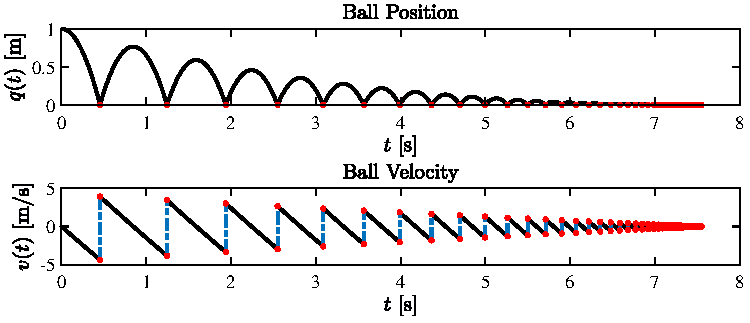
\includegraphics[width=\linewidth]{Figures/bb1.pdf}
        \caption[Time evolution of the ball bouncing on the actuated platform (autonomous case)]{Time evolution of the ball bouncing on the actuated platform (autonomous case).}
        \label{fig:bb1}
    \end{figure}
    %
\end{exmp}
%
%\begin{exmp}[Sliding mode controller]
%\textcolor{red}{to be completed...}
%\end{exmp}
%
\subsection{Stability}
%
Lyapunov stability theorems has been indeed extended to the hybrid case. In the case of continuous--time dynamical systems, the stability of equilibrium points is commonly discussed. However, in case of hybrid systems, it is rather convenient to analyze the stability of a set. Hereafter the very basic results on Lyapunov stability of hybrid systems will be introduced.
%
\begin{thm}[Lyapunov Stability for Hybrid Systems \citep{goebel2009hybrid}]\label{thm:hybrid_Lyap}
	%
	Let us consider an autonomous hybrid system $\left(\C,\F,\D,\G\right)$ and a compact set $\A\subset\R^n$ satisfying $\G\left(\D\cap\A\right)\subset\A$. If there exists a Lyapunov function candidate $V:\C\cup\D\rightarrow\R$ such that:
	\begin{subequations}
		\begin{align}
		&V(\xb)>0&&\forall \xb\in \left(\C\cup\D\right)\setminus\A\label{eq:stabh_1}\\
		&\langle\frac{\partial V}{\partial \xb},\mathbf{f}(\xb)\rangle\leq 0&&\forall \xb\in\C\setminus\A,\mathbf{f}\in\F\label{eq:stabh_2}~~~,\\
		&V(\mathbf{g}(\xb)) - V(\xb)\leq 0 &&\forall \xb\in\D\setminus\A,\mathbf{g}\in\G\label{eq:stabh_3}
		\end{align}
	\end{subequations}
	%
	then the set $\A$ is stable.
\end{thm}
%
\begin{cor}[\cite{goebel2009hybrid}]$\newline$
	Let $\Gamma_\mu := \left\{x\in\C\cup\D:V(x) = \mu\right\}$. If there exists a compact neighborhood $\K$ of $\A$ such that, for all $\mu>0$, no solution of the system remains in $\Gamma_\mu\cap\K$, then the set $\A$ is pre-asymptotically stable. In this case the basin of pre-attraction contains every compact set contained in $\K$ that is forward invariant.
\end{cor}
%
\begin{exmp}[Ball bouncing on actuated platform]
Let consider the autonomous case (u=0) and let 
%
\begin{equation}
    \A\triangleq \left\{(q,v)~:~q\leq\delta q\in\R^+\land |v|\leq\delta v\in\R^+\right\}.
\end{equation}
%

Indeed it holds 
%
\begin{equation}
    \A\cap\D = \left\{(0,v)~:~v\leq 0\land |v|\leq\delta v\in\R^+\right\}
\end{equation}
%
and
%
\begin{equation}
    \G\left(\A\cap\D\right) = \left\{(0,-cv)~:~v\leq 0\land |v|\leq\delta v\in\R^+\right\}\subset \A.
\end{equation}
%

Let's examine the stability of $A$. By choosing as Lyapunov function the energy of the system: $V(\xb) = \Ha(\xb)$. It holds, $\Ha(\xb)>0~~\forall \xb\in\left(\C\cup\D\right)\setminus\A$ and
%
\begin{align}
    \langle\frac{\partial\Ha}{\partial \xb},\F(\x)\rangle &= [m\gamma,mv]\begin{bmatrix}0&1\\0&-\beta/m\end{bmatrix}\begin{bmatrix}q\\v\end{bmatrix} + [m\gamma,mv] \begin{bmatrix}0\\-\gamma\end{bmatrix} \\
    & = -\beta v^2 \leq 0\quad\forall v\in\R,
\end{align}
%
which indeed holds for all $\xb\in\C\setminus\A$.
%
Finally, stability of $\A$ is proving noticing that
%
\begin{align}
    \Ha(\x^+) -\Ha(\xb) &= \frac{m}{2}(v^+)^2 + m\gamma q^+ - \frac{m}{2}v^2 + m\gamma q\\
    &= \frac{m}{2}(c-1)v^2\leq 0 \quad\forall v\in\R,~\forall c\in(0,1),
\end{align}
%
which holds also for any $\xb\in\D\setminus\A$. Note that in the case of the controlled system, $\A$ remains Lyapunov stable if and only if for all $t\geq 0$, $u(t)\leq c$. The descent of the energy during a trajectory of the system is represented in Fig. \ref{fig:bb2}.
%
\begin{figure}[!h]
    \centering
    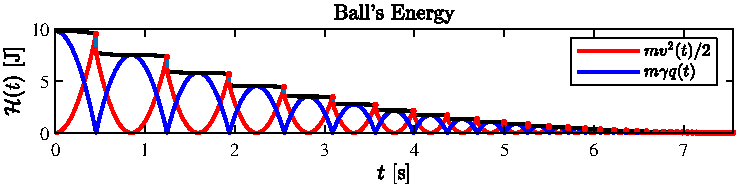
\includegraphics{Figures/bb2.pdf}
    \caption{Energy descent during a trajectory of the autonomous system.}
    \label{fig:bb2}
\end{figure}
%
\end{exmp}
%
% \begin{exmp}[Sliding mode controller]
% \textcolor{red}{to be completed...}
% \end{exmp}
%
\clearpage
%%%%%%%%%%%%%%%%%%%%%%%%%%%%%%%%%%%%%%%%%%%%%%%%%%%%%%%%%%%%%%%%%%%%%%%%%%%%%%%
\section{Summary}
 


%%\the\textwidth = 379.37pt
\definecolor{brickred}{rgb}{0.8, 0.25, 0.33}
\chapter{Hybrid Port--Hamiltonian Systems}

\label{chap:HPH_systems}
\minitoc

\thispagestyle{empty}

\newpage
%%%%%%%%%%%%%%%%%%%%%%%%%%%%%%%%%%%%%%%%%%%%%%%%%%%%%%%%%%%%%%%%%%%%%%%%%%%%%%%
\section{Introduction}
\lettrine[lines=4]{\color{brickred}H}{ereafter}, the framework of hybrid port--Hamiltonian systems will be introduced. Starting from the results discussed in Chapter \ref{chap:preliminaries}, the theories of port--Hamiltonian systems and hybrid inclusions will be merged. 
%
Previous attempts of modeling \textit{nonsmooth} system in a port--Hamiltonian fashion exist. 
%
\newline

%
In particular, \citep{valentin2006hybrid,valentin2007port} proposed a model for physical switching systems in an \textit{implicit} port--Hamiltonian fashion using \textit{network graph theory} and geometric considerations on the interconnection structure with main practical application to switching electrical circuits. An energy--based method for a class of (mechanical) impulsive port--Hamiltonian systems was also proposed in \cite{haddad2003energy}. Finally, \cite{Ishikawa2003} described a hopping robot by employing a port--Hamiltonian formulation.
%
\newline

%
Besides, the above mentioned works are mostly \textit{ad hoc} solutions and do not provide a \textit{big picture} of the framework. 
Indeed, a unified framework capable of capturing the intrinsic properties of a broad range hybrid dynamic phenomena from an energetic point of view, is still missing.
%
\newline

%
Firstly, the \textit{impulsive port--Hamiltonian systems} will be characterized. It is a generalization of single--flowed hybrid inclusions in a port--Hamiltonian fashion. This class of system is relevant to this study as most mechanical systems exhibiting (partially) elastic impacts, including robotics applications, belong to this framework. 
%
\newline

%
Afterwards, the general \textit{hybrid port--Hamiltonian system} will be defined. Examples for both classes of the proposed models will be provided.
%
\newline

%
Then, the concept of passivity will be extended to the hybrid case in the port--Hamiltonian context. Finally Lyapunov stability theorem is also extended from the one of hybrid inclusions. 
%
\clearpage
%%%%%%%%%%%%%%%%%%%%%%%%%%%%%%%%%%%%%%%%%%%%%%%%%%%%%%%%%%%%%%%%%%%%%%%%%%%%%%%
\section{Definitions and Basic Assumptions}
%%%%%%%%%%%%%%%%%%%%%%%%%%%%%%%%%%%%%%%%%%%%%%%% 
\subsection{Impulsive Port--Hamiltonian Systems}
%
Consider the single--flow specialization of the hybrid inclusion (\ref{eq:hs}):
%
\begin{equation}\label{eq:hs_singleflow}
    %
    \left\{ 
        \begin{matrix*}[l]\vspace{1pt}
            %
            \dot{\xb} = \mathbf{f}(\xb,\ub) && (\xb,\ub)\in\C\times\U\\
            \xb^+ \in \G(\xb)&&\quad~~\xb\in\D\\
            \yb = \mathbf{h}(\xb)
            %
        \end{matrix*}
    \right.~~,
    %
\end{equation}
%    
with $\mathbf{f}:\R^n\times\R^m\rightarrow\R^n$.
Here it is assumed that inputs enter into the dynamics only during flows and not during jumps. Therefore, 
%
\begin{equation}
    \ub\triangleq\ub_c,~~\U\triangleq\U_c.
\end{equation}
%

This assumption has been made to simplify the model since in most physical systems, no impulsive forcing terms can be practically applied.
%
\begin{defn}[Impulsive port--Hamiltonian Systems]
%
An impulsive port--Hamiltonian system is a system in the form (\ref{eq:hs_singleflow})  with port--Hamiltonian flows and output, i.e.
%
\begin{equation}\label{eq:impulsive_ph}
    %
    \boxed{
    \left\{ 
        \begin{matrix*}[l]\vspace{1pt}
            %
            \dot{\xb} = \left[\Jb(\xb)-\Rb(\xb)\right]\dH(\xb) + \Gb(\xb)\ub && (\xb,\ub)\in\C\times\U\\
            \xb^+ \in \G(\xb)&&\quad~~ \xb\in\D\\
            \yb = \Gb^\top(\xb)\dH(\xb)
            %
        \end{matrix*}
    \right.~~.
    }
    %
\end{equation}
%

The state--space of the system is $\X\triangleq\C\cup\D$ and $\Ha:\X\rightarrow\R$.
\end{defn}
%
An example of this type of systems is the \textit{ball--dribbling} and \textit{ball--juggling} robots of Fig. \ref{fig:1D}. Note that most mechanical systems exhibiting impacts admit a representation in the form (\ref{eq:impulsive_ph}).
%
\begin{exmp}[Impact Pendulum]\label{ex:ipend}
    Consider an impact pendulum of mass $m$ and length $\ell$ as in Fig. \ref{fig:ipend}.
    %
    \begin{figure}
        \centering
        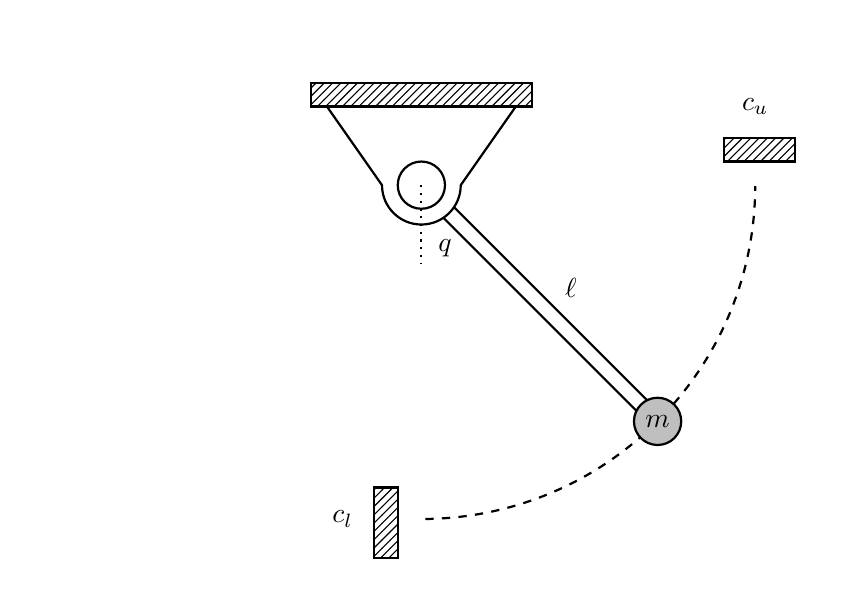
\begin{tikzpicture}[thick,>=latex,->]

\begin{scope}
\clip(-5,2) rectangle (5,-5);

\draw[dashed] (0,0)  circle (4.24cm);
\filldraw[white] (-4.3,4.3) rectangle (4.3,0);
\filldraw[white] (-4.3,4.3) rectangle (0,-4.3);


\draw[double distance=1.6mm] (0,0) -- (3,-3) node[midway,xshift=4mm,yshift=2mm]{$\ell$};
\draw[fill=white] (-1.2,1.0) -- (-.5,0) arc(180:360:0.5) -- (1.2,1.0) -- cycle;
\draw[draw=black,fill=white] (0, 0) circle circle (.3cm);
\draw[draw=black,fill=gray!50] (3,-3) circle circle (.3cm);
\draw[-,dotted] (0,0) -- (0,-1);

\draw[pattern=north east lines] (-1.4,1.3) rectangle (1.4,1);
\node at (.3,-.8) {$q$};   

\draw[-] (3,-3) node[] {$m$};
\draw[pattern=north east lines] (-.6,-4.74) rectangle (-.3,-3.84);
\draw[pattern=north east lines] (3.84,.3) rectangle (4.74,.6);
\draw[-] (-1,-4.24) node[] {$c_l$};
\draw[-] (4.24,1) node[] {$c_u$};
\end{scope}

\end{tikzpicture}
        \caption[Impact pendulum]{Impact pendulum of mass $m$ and length $\ell$. The systems has two impacts, one when the pendulum is at the resting position ($q=0$) and at $q = \pi/2$.}
        \label{fig:ipend}
    \end{figure}
    %
    Let $q$ be the pendulum angle and $p \triangleq m \ell^2 \dot{q}$ its angular momentum. The flows of the system are:
    %
    \begin{equation}
        %
        \dot{q} = \frac{1}{m\ell^2}p \quad
        \dot{p} = -m\gamma\ell\sin(q)-\frac{\beta}{m\ell^2}p + u,
        %
    \end{equation}
    %
    where $u$ is the input torque applied at the joint, $\gamma$ is the gravitational constant and $\beta$ is the viscous friction coefficient in the joint. The system admits an impulsive port--Hamiltonian form (\ref{eq:impulsive_ph}) with state $\xb\triangleq(q,p)$. In particular, the flows are described by the system matrices:
    %
    \begin{equation}
        \Jb\triangleq\begin{bmatrix}0&1\\-1&0\end{bmatrix},~~\Rb\triangleq \begin{bmatrix}0&0\\0&\beta\end{bmatrix},~~\Gb\triangleq\begin{bmatrix}0\\1\end{bmatrix}.
    \end{equation}
    %
    
    The Hamiltonian function is 
    %
    \begin{equation}
        \Ha(q,p)\triangleq\frac{1}{2m\ell^2}p^2 + mg\ell(1-\cos(q)).
    \end{equation}
    %
    
    The systems has two impacts, one when the pendulum is at the resting position ($q=0$) and at $q = \pi/2$. Thus,
    %
    \begin{align}
        &\xb^+ = \mathbf{g}_1(\xb) \triangleq \overbrace{\begin{bmatrix}1&0\\0&-c_l\end{bmatrix}}^{\mathbf{M}_1}\xb\quad\text{if}\quad\xb\in\D_1\triangleq\left\{\xb:q=0\land p\leq 0\right\} \\
        %
        &\xb^+ = \mathbf{g}_2(\xb) \triangleq \underbrace{\begin{bmatrix}1&0\\0&-c_u\end{bmatrix}}_{\mathbf{M}_2}\xb\quad\text{if}\quad\xb\in\D_2\triangleq\left\{\xb:q=\pi/2\land p\geq 0\right\}
    \end{align}
    %
    and, therefore,
    %
    \begin{equation}
        \G\triangleq\left\{\mathbf{g}_i:\xb\in\D_i\Rightarrow\xb^+ = \mathbf{g}_i(\xb),~i = 1,2\right\}.
    \end{equation}
    %
    \end{exmp}
%
\subsection{Hybrid port--Hamiltonian Systems}
%

This thesis deals with systems which present a finite number of modes and thus, can be described through an \textit{hybrid automata} (see \cite{van2000introduction}). However, it is convenient to describe them as hybrid inclusions in the form (\ref{eq:hs}). In \citep{goebel2009hybrid} an hybrid inclusion formulation of hybrid automata is given. However, the formulation of hybrid port--Hamiltonian systems will be derived starting from the notion of impulsive port--Hamiltonian system.

Let us consider a dynamical systems which behavior is the collection of $r$ ``modes'' in the form (\ref{eq:impulsive_ph}), i.e.
%
\begin{equation}
    %
    \left\{ 
        \begin{matrix*}[l]\vspace{1pt}
            %
            \dot{\xb} = \left[\Jb_s(\xb)-\Rb_s(\xb)\right]\dH_s(\xb) + \Gb_s(\xb)\ub && (\xb,\ub)\in\C_s\times\U\\
            \xb^+ \in \G_s(\xb)&&\quad~~ \xb\in\D_s\\
            \yb = \Gb_s^\top(\xb)\dH_(\xb)
            %
        \end{matrix*}\qquad s\in\M 
    \right.~~,
    %
\end{equation}
%
where $\M\triangleq\mathbb{N}^*_{\leq r}$. The transition between one mode and another may happen only during jumps. Therefore, a state extension might be performed to include the mode index in the state:
%
\begin{equation}
    \zb \triangleq (\xb,s).
\end{equation}
%

Let us now define the port--Hamiltonian flow set--valued mapping as
%
\begin{equation}\label{eq:hph_flowmap}
    \F_{\tt PH}(\xb,\ub) \triangleq \F(\xb,\ub)\times\{0\},
\end{equation}
%
where
%
\begin{equation}
    \F\triangleq\left\{\mathbf{f}_i(\xb,\ub) = \left[\Jb_i(\xb)-\Rb_i(\xb)\right]\dH_i(\xb) + \Gb_i(\xb)\ub~:~(\xb,s)\in\C_i\times\{i\}\Rightarrow \dot{\xb} = \mathbf{f}_i(\xb,\ub)\right\}.
\end{equation}
%

The flow set can be then defined as
%
\begin{equation}
    \C\triangleq\bigcup_{s\in\M}\left(\C_s\times\{s\}\right).
\end{equation}
%

Note that the jump set $\D_s$ and the jump map $\G_s(\xb)$ of each mode enjoy the following:
%
\begin{equation}
    \D_s\triangleq \bigcup_{i\in\M}\D_{s\Arrow{0.1cm} i}~~\text{ and }~~\G_s(\xb)\triangleq \bigcup_{i\in\M}\G_{s\Arrow{0.1cm}i}(\xb),
\end{equation}
%
such that 
%
\begin{equation}
    %
    \begin{bmatrix}
        \xb^+\\
        s^+    
    \end{bmatrix}
    %
    \in
    %
    \G_{s\Arrow{0.1cm}i}(\xb)\times\{i\}
    %
    %\begin{bmatrix}
    %    \mathbf{g}_{s\Arrow{0.1cm}i}(\xb)\\
    %    i    
    %\end{bmatrix}
    %
    \qquad (\xb,s)\in\D_{s\Arrow{0.1cm}i}\times\{s\}.
\end{equation}
%

The port--Hamiltonian jump set--valued mapping is then defined as
%
\begin{equation}\label{eq:hph_jumpmap}
    \G_{\tt PH}(\x) \triangleq\bigcup_{s\in\M,~i\in\M}\left(\G_{s\Arrow{0.1cm}i}(\xb),~i\right),
\end{equation}
%
while the jump set as
%
\begin{equation}\label{eq:hph_jumpset}
    \D \triangleq \bigcup_{s\in\M}\left(\D_s\times\{s\}\right).
\end{equation}
%

If the output set valued mapping is also defined as
%
\begin{equation}
    \Oo_{\tt PH} \triangleq \left\{\mathbf{h}_i(\xb) = \mathbf{G}_i^\top(\xb)\dH(\xb)~:~(\xb,s) \in\C_s\times\{i\}\Rightarrow y=\mathbf{h}_i(\xb)\right\},
\end{equation}
%
the formulation of \textit{hybrid port--Hamiltonian system} is the following:
%
\begin{equation}\label{eq:hph}
    \boxed{
    \left\{
        %
        \begin{matrix*}[l]
            %
            (\dot{\xb},\dot{s}) \in \F_{\tt PH} & (\xb,s)\in\C\\
            %
            (\xb^+,s^+) \in \G_{\tt PH} & (\xb,s)\in\D\\
            %
            y \in \Oo_{\tt PH}
            %
        \end{matrix*}
        %
    \right.~~.
    }
\end{equation}
%
\begin{rem}
	The output of both impulsive and  hybrid port--Hamiltonian system is defined only during flows for two main reasons. Firstly, jumps occurrences are assumed to happen in zero--measure time intervals. Moreover, it is also assumed that no inputs are applied during jumps and, hence, undefined outputs cannot broke duality.
\end{rem}
%
\begin{exmp}[Hopping Robot on elastic ground.]\label{ex:hopping}
    %
    Consider the hopping robot on elastic ground represented in Fig. \ref{fig:hopping} and inspired by \cite{Ishikawa2003}.
    %
    \begin{figure}[h]
        \centering
        \definecolor{ocean}{rgb}{0.00000,0.44700,0.74100}
%
\begin{tikzpicture}[scale=1, every node/.style={scale=1}]
        \tikzstyle{spring}=[thick,decorate,decoration={zigzag,pre length=0.3cm,post length=0.3cm,segment length=6}]
        \tikzstyle{damper}=[thick,decoration={markings,  
            mark connection node=dmp,
            mark=at position 0.5 with 
            {
                \node (dmp) [thick,inner sep=0pt,transform shape,rotate=-90,minimum width=15pt,minimum height=3pt,draw=none] {};
                \draw [thick] ($(dmp.north east)+(2pt,0)$) -- (dmp.south east) -- (dmp.south west) -- ($(dmp.north west)+(2pt,0)$);
                \draw [thick] ($(dmp.north)+(0,-5pt)$) -- ($(dmp.north)+(0,5pt)$);
            }
        }, decorate]
        \tikzstyle{ground}=[fill,pattern=north east lines,draw=none,minimum width=0.75cm,minimum height=0.3cm,inner sep=0pt,outer sep=0pt]

        \node [draw, outer sep=0pt,thick,fill = gray!50] (M) [minimum width=2cm, minimum height=.3cm] {$m_1$};
        %
        \node [draw, outer sep=0pt,thick,fill = gray!50] (M2) [minimum width=2cm, minimum height=.3cm, yshift =-2cm] {$m_2$};
        %
        \node [draw, outer sep=0pt, thick,fill = gray] (M3) [minimum width=2cm, minimum height=0.1cm, yshift =-3.5cm] {};
        
        \draw [damper] (M.200) -- ($(M2.north west)!(M.200)!(M2.north east)$);
        \draw [spring] (M.340) -- ($(M2.north west)!(M.340)!(M2.north east)$);
        \draw [-,thick] (M.270) -- ($(M2.north west)!(M.270)!(M2.north east)$);
        \draw[draw=black,fill=ocean!50,thick] (0,-1cm) circle (0.25cm);
        
        \node (b) at (M2.north) [xshift = -1.2cm, yshift = 0.75cm] {$b$};
        \node (k) at (M2.north) [xshift = 1.2cm, yshift = 0.75cm] {$k$};
        \node (u) at (M2.north) [xshift = 0cm, yshift = 0.75cm] {$u$};
        
        \node (ground2) [ground,anchor=north,yshift=-2.25cm,minimum width=4cm,xshift=0cm] at (M2.south) {};
        \draw (ground2.north east) -- (ground2.north west);
        \draw (ground2.south east) -- (ground2.south west);
        \draw (ground2.north east) -- (ground2.south east);
        \draw (ground2.north west) -- (ground2.south west);
        
        \draw [spring] (ground2.20) -- ($(M3.south west)!(ground2.20)!(M3.south east)$);
        \draw [damper] (ground2.160) -- ($(M3.south west)!(ground2.160)!(M3.south east)$);
        
        \node (b) at (M3.south) [xshift = -1cm, yshift = -0.5cm] {$b_g$};
        \node (k) at (M3.south) [xshift = 1cm, yshift = -0.5cm] {$k_g$};
        %
        \draw[->, very thick] (ground2.west) -- (-2,1);
        \draw[-, dotted] (M.south west) -- +(-1,0cm);
        \draw[-, dotted] (M2.south west) -- +(-1,0cm);
        \draw[-, dotted] (M3.north west) -- +(-1,0cm);
        \node (q1) at (M.south west) [xshift = -1.3cm] {$q_1$};
        \node (q2) at (M2.south west) [xshift = -1.3cm] {$q_2$};
        \node (q3) at (M3.north west) [xshift = -1.6cm] {$q_3\equiv 0$};
        %%%%%%%%%%%%%%%%%%%%%%%%%%%%%%%%%%%%%%%
        \node [draw, outer sep=0pt,thick,fill = gray!50] (M) [minimum width=2cm, minimum height=.3cm,xshift = 5cm,yshift =-1.2cm] {$m_1$};
        %
        \node [draw, outer sep=0pt,thick,fill = gray!50] (M2) [minimum width=2cm, minimum height=.3cm, xshift = 5cm, yshift =-3.2cm] {$m_2$};
        %
        \node [draw, outer sep=0pt, thick,fill = gray] (M3) [minimum width=2cm, minimum height=0.1cm, xshift = 5cm, yshift =-3.5cm] {};
        
        \draw [damper] (M.200) -- ($(M2.north west)!(M.200)!(M2.north east)$);
        \draw [spring] (M.340) -- ($(M2.north west)!(M.340)!(M2.north east)$);
        \draw [-,thick] (M.270) -- ($(M2.north west)!(M.270)!(M2.north east)$);
        \draw[draw=black,fill=ocean!50,thick] (5cm,-2.2cm) circle (0.25cm);
        
        \node (b) at (M2.north) [xshift = -1.2cm, yshift = 0.75cm] {$b$};
        \node (k) at (M2.north) [xshift = 1.2cm, yshift = 0.75cm] {$k$};
        \node (u) at (M2.north) [xshift = 0cm, yshift = 0.75cm] {$u$};
        
        \node (ground2) [ground,anchor=north,yshift=-1.05cm,minimum width=4cm,xshift=0cm] at (M2.south) {};
        \draw (ground2.north east) -- (ground2.north west);
        \draw (ground2.south east) -- (ground2.south west);
        \draw (ground2.north east) -- (ground2.south east);
        \draw (ground2.north west) -- (ground2.south west);
        
        \draw [spring] (ground2.20) -- ($(M3.south west)!(ground2.20)!(M3.south east)$);
        \draw [damper] (ground2.160) -- ($(M3.south west)!(ground2.160)!(M3.south east)$);
        
        \node (b) at (M3.south) [xshift = -1cm, yshift = -0.5cm] {$b_g$};
        \node (k) at (M3.south) [xshift = 1cm, yshift = -0.5cm] {$k_g$};
        
        \node (fly) at (0,0) [xshift = 0cm, yshift = 1cm] {\textbf{Non--Contact Mode}};
        \node (fly) at (5cm,0) [xshift = 0cm, yshift = 1cm] {\textbf{Contact Mode}};
        
\end{tikzpicture}
        \caption[Hopping robot on elastic ground]{Hopping robot on elastic ground. }
        \label{fig:hopping}
    \end{figure}
    %
    The \textit{robot} is made up of two masses interconnected with a spring of stiffness $k$ and resting length $\ell$, a dashpot with damping coefficient $b$ and a linear actuator which exerts an axial force $u$ (input to the system). 
    $q_1,~q_2$ are the absolute height of the masses.
    
    The plate where the robots ``hops'' is assumed to be massless and connected to the ground with a spring of stiffness $k_g$ and a dashpot of damping coefficient $b_g$.
    $q_3$ is the position of the plate and assumed to be zero at rest.
    
    Finally, impacts are considered completely inelastic and that takeoff from ground always happens at $q_2 = q_3 = 0$.
    
    The system has two modes ``Contact'' and ``Non--contact''. The flows in contact/non--contact modes are, respectively:
    %
    \begin{align}
        %
        \text{non--contact}\quad
        %
        &\left\{
            \begin{matrix*}[l]
            %
            m_1\ddot{q}_1 = -m_1\gamma -k\left(q_1-q_2-\ell\right) -b\left(\dot{q}_1-\dot{q}_2\right) + u\\
            %
            m_2\ddot{q}_2 = -m_2\gamma +k\left(q_1-q_2-\ell\right) +b\left(\dot{q}_1-\dot{q}_2\right) - u\\
            %
            \ddot{q}_3 = 0
            \end{matrix*}
        \right.~~,\\
        %%
        \text{contact}\quad
        %
        &\left\{
            \begin{matrix*}[l]
            %
            m_1\ddot{q}_1 = -m_1\gamma -k\left(q_1-q_2-\ell\right) -b\left(\dot{q}_1-\dot{q}_2\right) + u\\
            %
            m_2\ddot{q}_2 = -m_2\gamma +k\left(q_1-q_2-\ell\right) +b\left(\dot{q}_1-\dot{q}_2\right) - k_gq_3-b_g\dot{q}_3 - u\\
            %
            \ddot{q}_3 = \dot{q}_2
            \end{matrix*}
        \right.~~.
        %
    \end{align}
    %
    
    Let $s$ be the mode index and let $s=1$ in ``non--contact'' while $s=2$ in contact modes. Moreover, let $\qb \triangleq (q_1,q_2,q_3)$, $\pb\triangleq (m_1q_1,m_2q_2)$ and $\xb\triangleq(\qb,\pb)$. The flows of the two system modes can be then transformed in port--Hamiltonian form with the following system matrices:
    %
    \begin{equation}
        %
        \Jb_1\triangleq
        \begin{bmatrix}
            %
            0&0&0&1&0\\
            0&0&0&0&1\\
            0&0&0&0&0\\
            -1&0&0&0&0\\
            0&-1&0&0&0\\
            %
        \end{bmatrix},~~
        %
        \Rb_1\triangleq
        \begin{bmatrix}
            %
            0&0&0&0&0\\
            0&0&0&0&0\\
            0&0&0&0&0\\
            0&0&0&b&-b\\
            0&0&0&-b&b\\
            %
        \end{bmatrix},~~
        %
        \Gb_1\triangleq
        \begin{bmatrix}
            %
            0\\0\\0\\1\\-1
            %
        \end{bmatrix},
        %
    \end{equation}
    %%
    \begin{equation}
        %
        \Jb_2\triangleq
        \begin{bmatrix}
            %
            0&0&0&1&0\\
            0&0&0&0&1\\
            0&0&0&0&1\\
            -1&0&0&0&0\\
            0&-1&-1&0&0\\
            %
        \end{bmatrix},~~
        %
        \Rb_2\triangleq
        \begin{bmatrix}
            %
            0&0&0&0&0\\
            0&0&0&0&0\\
            0&0&0&0&0\\
            0&0&0&b&-b\\
            0&0&0&-b&b+b_g\\
            %
        \end{bmatrix},~~
        %
        \Gb_2\triangleq
        \begin{bmatrix}
            %
            0\\0\\0\\1\\-1
            %
        \end{bmatrix},
        %
    \end{equation}
    %
    and Hamiltonian functions
    %
    \begin{align}
        &\Ha_1(\xb) \frac{1}{2}\triangleq \pb^\top\begin{bmatrix}m_1&0\\0&m_2\end{bmatrix}^{-1}\pb + \frac{1}{2}k\left(q_1-q_2-\ell\right)^2 + \gamma[m_1,m_2]\qb, \\
        %
        &\Ha_2(\xb) \frac{1}{2}\triangleq \pb^\top\begin{bmatrix}m_1&0\\0&m_2\end{bmatrix}^{-1}\pb + \frac{1}{2}k\left(q_1-q_2-\ell\right)^2 + \frac{1}{2}k_g q_3^2+ \gamma[m_1,m_2]\qb.
    \end{align}
    %
    
    The port--Hamiltonian flow set--valued mapping can be then defined as in (\ref{eq:hph_flowmap}). The two flows happen, respectively if 
    %
    \begin{align}
        &(\xb,s)\in\C_1\times\{1\}\triangleq\left\{\xb~:~\q_2>0\right\}\times\{1\},\\
        &(\xb,s)\in\C_2\times\{2\}\triangleq\left\{\xb~:~\q_2\leq0\right\}\times\{2\}.
    \end{align}
    %
    
    Transitions between the two modes happen as follows:
    %
    \begin{align}
        &\begin{bmatrix}\xb^+\\s^+\end{bmatrix} = \begin{bmatrix}\xb\\2\end{bmatrix}\quad\text{if}\quad(\xb,s)\in\D_1\times\{1\}\triangleq\{\xb:q_2\leq 0\}\times\{1\},\\
        %
        &\begin{bmatrix}\xb^+\\s^+\end{bmatrix} = \begin{bmatrix}\xb\\1\end{bmatrix}\quad\text{if}\quad(\xb,s)\in\D_2\times\{2\}\triangleq\{\xb:q_2> 0\}\times\{2\}.
    \end{align}
    %
    
    Thus, the jump set and the jump set--valued mapping can be derives as in (\ref{eq:hph_jumpset}), (\ref{eq:hph_jumpmap}).
    Finally, it can be noticed that the output is the same for each mode:
    %
    \begin{equation}
        y = \Oo_{\tt PH}\triangleq\Gb_1^\top\dH_1(\xb) = \Gb_2^\top\dH_2(\xb) = \dot{q}_1 - \dot{q}_2. 
    \end{equation}
    %
\end{exmp}
%
%
The concept of passivity, fundamental for the
theory port-Hamiltonian systems, can be extended to
the hybrid case in the following section.
%
\clearpage
%
%%%%%%%%%%%%%%%%%%%%%%%%%%%%%%%%%%%%%%%%%%%%%%%%%%%%%%%%%%%%%%%%%%%%%%%%%%%%%%%
\section{Passivity}
%
The concept and characterization of passivity for hybrid systems has been recently explored by \cite{naldi2013passivity}.
%
\begin{defn}[Passive impulsive port--Hamiltonian system]\label{def:impulsive_passivity}
    %
    A system in the form (\ref{eq:impulsive_ph}) is passive if and only if it satisfies the following dissipation inequality
    %
    \begin{equation}
        \forall\xb\in\D,~\mathbf{g}\in\G \quad \Ha(\mathbf{g}(\xb))-\Ha(\xb)\leq 0.
    \end{equation}
    %
\end{defn}
%
Hereafter, necessary and sufficient condition for the passivity of a subclass systems of type (\ref{eq:impulsive_ph}) is given. Firstly, let us start with a basic definition.
%
\begin{defn}[Evenly $\bm\psi$--diverging function]
	Let $\bm\psi:\R^n\supseteq\dom(\bm\psi)\rightarrow\R^n$. A map $\Ha:\R^n\supseteq\dom(\Ha)\rightarrow\R$ is evenly diverging with respect to $\bm\psi$ if
	%
	\begin{equation}
	    \forall\bm\xi\in\dom(\bm\psi)~~\Ha(\bm\psi(\bm\xi))-\Ha(\bm\xi)\leq 0 \Leftrightarrow \|\bm\psi(\bm\xi)\|_2-\|\bm\xi\|_2\leq {0}.
	\end{equation}
	%
\end{defn}
%
\begin{prop}[Condition for passivity of impulsive port--Hamiltonian systems]\label{prop:pass_impulsive}
	%
	Without any loss of generality, let us assume $\mymathbb{0}$ to be a minimum of $\Ha(\xb)$:
	%
	\begin{equation}
	    \mymathbb{0}_n = \min_{\x\in\X}\Ha(\xb).
	\end{equation}
	%
	
	A system (\ref{eq:impulsive_ph}) such that $\Ha(\xb)$ is positive in $\X\setminus\{\mymathbb{0}_n\}$, $\Ha(\mymathbb{0}_n)=0$ and $\Ha$ is evenly diverging with respect to all $\mathbf{g}\in\G$, is passive if and only if 
	%
	\begin{equation}\label{eq:nl_pass}
		\|\mathbf{g}\|_\infty\leq 1\quad\forall \mathbf{g}\in\G.
	\end{equation}
	%
\end{prop}
%
\begin{proof}
	If $\Ha(\xb)$ is evenly diverging with respect to all the jump maps, it holds
	%
	\begin{align}
	    \forall\mathbf{g}\in\G,~\xb\in\X\quad\Ha(\mathbf{g}(\xb))-\Ha(\xb)\leq 0 \Leftrightarrow \|\mathbf{g}(\xb)\|_2 \leq \|\xb\|_2.
	\end{align}
	%
	
	Then,
	%
	\begin{align*}
	\Ha(\mathbf{g}(\xb))-\Ha(\xb)\leq 0 \quad \Leftrightarrow \quad \sup\limits_{\xb\neq 0}\frac{\|\mathbf{g}(\xb)\|_2}{\|\xb\|_2} \triangleq \|\mathbf{g}\|_\infty\leq 1.
	\end{align*}
    %
\end{proof}
%
If $\mathbf{g}$ is a linear function, i.e. $\mathbf{g}(\xb) = \mathbf{M}\xb$ ($\mathbf{M}\in\R^{n\times n}$), condition (\ref{eq:nl_pass}) requires that the maximum among the absolute value of the eigenvalues of $\mathbf{M}$ is less or equal than one:
%
\begin{equation}
	\forall k \in\mathbb{N}^*_{\leq n} \qquad \max\limits_{k}|\lambda_k|_2\leq 1\quad\lambda_k:\mathbf{M}\mathbf{v}_k = \lambda_k\mathbf{v}_k.
\end{equation}
%

Note that this Proposition can be naturally extended to the case in which $\Ha$ has a unique minimum in $\xb^*$ by a change of coordinates $\zb\triangleq \xb-\xb^*$ and requiring $\Ha \circ~\zb:\X\rightarrow\R$ to be evenly diverging with respect to all $\gb\in\G$.
%
\newline

%
Here, passivity corresponds to the property of no internal energy generation during jumps. In fact, during flows, the (continuous time) passivity is guaranteed by the port--Hamiltonian structure.
Note that Definition \ref{def:impulsive_passivity} is analogous to the one of \textit{flow-passivity} in \cite{naldi2013passivity} applied to single--flows hybrid inclusions with port--Hamiltonian flows. 
%
\begin{rem}
    Recalling, example \ref{ex:ipend}, it can be concluded that the impact pendulum model is passive for Proposition \ref{prop:pass_impulsive} if and only if the restitution coefficients $c_l$, $c_u$ are all less then one.
\end{rem}
%
Passivity can also be defined for hybrid port--Hamiltonian systems by extending Definition \ref{def:impulsive_passivity} as follows.
%
\begin{defn} [Passive hybrid port--Hamiltonian system]\label{def:hybrid_passivity}
    %
    A system in the form (\ref{eq:hph}) is passive if and only if it satisfies the following dissipation inequality
    %
    \begin{equation}
        \forall s\in\M,~i\in\M,~\xb\in\D_{s\Arrow{0.1cm}i},~\mathbf{g}\in\G_{s\Arrow{0.1cm}i} \quad \Ha_i(\mathbf{g}(\xb))-\Ha_s(\xb)\leq 0.
    \end{equation}
    %
\end{defn}
%
Similarly, Proposition \ref{prop:pass_impulsive} can be also naturally extended to hybrid case. Note that this definition is consistent to the definition of dissipative hybrid automata in \citep{agarwal2017}. 
%
%\begin{prop}[Condition for passivity of hybrid port--Hamiltonian systems]\label{prop:pass_hybrid}
%    %
%	Let us assume
%	%
%	\begin{equation}
%	    \forall s\in\M\quad \mymathbb{0}_n = \min_{\x\in\X}\Ha_s(\xb).
%	\end{equation}
%	%
%	
%	A system (\ref{eq:hph}) such that 
%	%
%	\begin{equation}
%	    \forall s\in\M~~\left(\xb\in\X\setminus\{\mymathbb{0}_n\}\Rightarrow\Ha_s(\xb)>0\right) \land\Ha_s(\mymathbb{0}_n)=0,
%	\end{equation}
%	%
%	and, for all $s$, $\Ha_s$ is evenly diverging with respect to all $\mathbf{g}_s\in\G_s$, is passive if and only if 
%	%
%	\begin{equation}%\label{eq:nl_pass}
%		\forall s\in\M,~\mathbf{g}_s\in\G\quad\|\mathbf{g}_s\|_\infty\leq 1.
%	\end{equation}
%	%
%\end{prop}
%%
%\begin{proof}
%    The proof follows naturally the one of Proposition \ref{prop:pass_impulsive}.
%\end{proof}
%
\begin{rem}
The hopping robot of Example \ref{ex:hopping} is passive since the jump maps are simply the identity and, thus, there is no energy variation during jumps (jump--lossless). 
\end{rem}
%
Lyapunov stability of both, impulsive and hybrid port--Hamiltonian systems, will be addressed in the next section.
%
\clearpage
%%%%%%%%%%%%%%%%%%%%%%%%%%%%%%%%%%%%%%%%%%%%%%%%%%%%%%%%%%%%%%%%%%%%%%%%%%%%%%%
\section{Lyapunov Stability of Autonomous Systems}
%
The following theorem has been derived from Theorem \ref{thm:hybrid_Lyap}.
%
\begin{thm}[Lyapunov Stability of Impulsive port--Hamiltonian Systems]\label{thm:impulsive_lyap}
    %
    Consider a system in the form (\ref{eq:impulsive_ph}) with $\ub = 0$ and a compact set $\A\subset\X$ satisfying $\G\left(\D\cap\A\right)\subset\A$. If
	%
	\begin{subequations}
		\begin{align}
		&\Ha(\xb)>0&&\forall x\in \left(\C\cup\D\right)\setminus\A\label{eq:stabhph_1},\\
		&\Ha(\gb(\xb)) - \Ha(\xb)\leq 0 &&\forall \xb\in\D\setminus\A,\forall \gb\in\G\label{eq:stabhph_3},
		\end{align}
	\end{subequations}
	%
	then the set $\A$ is stable.
	%
\end{thm}
%
\begin{proof}
    The proof is obtained directly from Theorem \ref{thm:hybrid_Lyap}. Firstly, let us assume $\Ha$ to be the candidate Lyapunov function. Then, conditions (\ref{eq:stabh_1}) and (\ref{eq:stabh_3}) correspond, respectively to (\ref{eq:stabhph_1}), (\ref{eq:stabhph_3}). Finally, condition (\ref{eq:stabh_2}) is automatically satisfied due to the port--Hamiltonian structure of the flows, i.e.
    %
    \begin{equation}
        \langle\dH(\xb),\dot{\xb}\rangle = \dH^\top(\xb)\Rb(\xb)\dH(\xb)\leq 0.
    \end{equation}
    %
    
    Thus, if the conditions of this Theorem are satisfied, the system is Lyapunov stable according to Theorem \ref{thm:hybrid_Lyap}. 
\end{proof}
%
Note that the condition (\ref{eq:stabhph_3}) is automatically satisfied if (\ref{eq:impulsive_ph}) is passive.
%
\begin{cor}\label{cor:impulsive_lyap}
	Consider a system in the form (\ref{eq:impulsive_ph}) and assume it to be passive. If
	%
	\begin{equation}
	\exists \xb^*~:~\forall \xb\neq \xb^*~~\Ha(\xb)>0\text{ },\quad\Ha(\xb^*) = 0,
	\end{equation}
	% 
	then, for any $\epsilon>0$ there exists a Lyapunov stable set
	%
	\begin{equation}
		\A_\epsilon = \left\{\xb:\Ha(\xb)\leq\epsilon\right\}.
	\end{equation}
	%
\end{cor}
%
Thus, every neighborhood of any strict minimum of $\Ha$ is stable as long as (\ref{eq:hph}) is passive.
%
\begin{rem}
    Regarding the impact pendulum of Example \ref{ex:ipend}, any neighborhood $\B_{o^+}$ of the origin,
    %
    \begin{equation}
        \B_{0^+}\triangleq \left\{(q,p)~:~0\leq q\leq\delta q\in\R^+\land0\leq p\leq\delta p\in\R^+\right\},
    \end{equation}
    %
    can be easily proven to be a Lyapunov stable set according to Theorem \ref{thm:impulsive_lyap}. Moreoever, thanks to Corollary \ref{cor:impulsive_lyap}, it can be deduced that for all nonnegative $\epsilon$, $\A_\epsilon$ is Lyapunov stable.
\end{rem}
%
It is trivial to extend also Lyapunov stability to the hybrid port--Hamiltonian case by means of multiple Lyapunov functions. However, only passive systems are worth to be considered. 

Minima of the Hamiltonian function are known to be asymptotically stable fixed points of port--Hamiltonian systems with non--null dissipation. Along any trajectory, the system will dissipate its energy eventually landing in one of the minima of the Hamiltonian. 

Nevertheless, this holds also for hybrid port--Hamiltonian systems\footnote{Here we are taking for granted well--posedness and regularity (maximality) of solutions.}. The main difference is that here energy is dissipated also during discrete jumps and thus, the state will eventually converge to one of the Hamiltonian minima of some system's mode.  

Finally, it can also be proven that, if there exists a point $\xb^*$ being the unique strict minimum of each mode's Hamiltonian function, then $\x^*$ is stable and globally attractive.
%

%
\clearpage
%%%%%%%%%%%%%%%%%%%%%%%%%%%%%%%%%%%%%%%%%%%%%%%%%%%%%%%%%%%%%%%%%%%%%%%%%%%%%%%
%\section{Some Extensions of Passivity--Based Control}
%\clearpage
%%%%%%%%%%%%%%%%%%%%%%%%%%%%%%%%%%%%%%%%%%%%%%%%%%%%%%%%%%%%%%%%%%%%%%%%%%%%%%%
\section{Summary}
%
In this chapter, hybrid port--Hamiltonian systems have been defined. Both passivity and stability have also characterized.
%
\newline

%
As a final consideration, this chapter left opened the utility of this modeling framework for real applications, either in robotics or control theory.
%
\newline

%
Following, in the next chapters several applications are proposed, ranging from the control a ball--dribbling robot to the hybrid control of linear systems. Note that, in the latter case, explored in Chapter \ref{chap:multistable}, the ``hybrid'' nature is not given by the physics of the system but from the controller.
%
%\definecolor{brickred}{rgb}{0.8, 0.25, 0.33}
%
\chapter{Iterative Energy Shaping of a Ball--Dribbling Robot}

\label{chap:multistable}
\minitoc

\thispagestyle{empty}

\newpage
%%%%%%%%%%%%%%%%%%%%%%%%%%%%%%%%%%%%%%%%%%%%%%%%%%%%%%%%%%%%%%%%%%%%%%%%%%%%%%%%%
\section{Introduction}
%
\lettrine[lines=4]{\color{brickred}C}{hallenging} control problems are often the best and most direct way to prove the validity of a modeling framework. In this chapter we present a novel method for controlling a \textit{ball--dribbling} robot.
A representation of the controlled system is given in Figure \ref{fig:1D}.
%
\begin{figure}[h]
    %
	\centering
	\definecolor{mycolor1}{rgb}{0.00000,0.44700,0.74100}%
\definecolor{ocean}{rgb}{0.00000,0.44700,0.74100}

\begin{tikzpicture}
	% axes
	\draw[thick] (0,0)--(3cm,0);
	\draw[dotted] (-.5,0.6cm) node[anchor = east] {\color{black}$0$}--(3cm,0.6cm);
	\draw[thick,dashed] (1.5cm,0) -- (1.5cm,3cm);
	\draw (0cm,0cm) -- (3cm,0) -- (3cm,3cm) -- (0cm,3cm) -- (0cm,0cm);
	% yaxis
	\draw[very thick,-latex] (-0.5,-.2) -- (-.5,3);  
	% robot
	\fill[ocean, draw = black,thick] (1,2.05) rectangle (2,2.65);
	% ball
	\fill[orange, draw=black,thick] (1.5,1.05) circle (0.3);
	%	
	%\draw[thick,->] (2,2.05) -- (2.25,2.05) -- (2.25,2.4) node[anchor=west] {$q_1$};
	%\draw[thick,->] (1,2.05) -- (0.75,2.05) -- (0.75,2.4) node[anchor=east] {$u$};
	%\draw[thick,->] (1.5,1.35) -- (2.25,1.35) -- (2.25,1.7) node[anchor=west] {$q_2$};
	%\draw[thick,->] (2,2.05) -- (2.25,2.05) -- (2.25,2.4) node[anchor=west] {$q_1$};
	%\draw[thick,->] (1,2.05) -- (0.75,2.05) -- (0.75,2.4) node[anchor=east] {$u$};
	%\draw[thick,->] (1.5,1.35) -- (2.25,1.35) -- (2.25,1.7) node[anchor=west] {$q_2$};
	%
	\draw[dotted] (1.5,1.35) -- (1,1.35);
	\draw[dotted] (1.5,0.75) -- (1,0.75);
	\draw[<->] (1,0.75) -- (1,1.35)  node[anchor=north east] {$2r$};
	%
	%\foreach \x in {0,0.25,0.5,0.75,1,1.25,1.5,1.75,2,2.25,2.5,2.75}
%	\draw[thick] (\x,-0.15) -- (\x+0.25,0);
	%
	\draw[pattern=north east lines] (0,-.2) rectangle (3,0);
	%
	\draw[dashed] (-.5,2.05)--(3.51cm,2.05);
	\draw[dashed] (-.5,1.35)--(3.51cm,1.35);
	\draw[-,dotted] (-.5, 0) -- (0, 0);
	%
	\node[] at (-.75, 2.05) {$q_1$};
	\node[] at (-.75, 1.35) {$q_2$};
	\node[] at (-.95, 0) {$-2r$};
	\draw[color=black, dotted, line width=1.5pt] (0,1.8)--(3,1.8);
	%%%%%%%%%%%%%%%%%%%%
	\begin{axis}[%
width=4cm,
height=3cm,
at={(3.5cm,0cm)},
scale only axis,
xmin=18.7,
xmax=20,
ymin=-0.5,
ymax=2,
ticks=none,
axis background/.style={fill=white},
legend style={legend cell align=left, align=left, draw=white!15!black}
]
\addplot [color=black, dotted, line width=0.5pt]
  table[row sep=crcr]{%
  18.65 0\\
  20 0\\
  };

\addplot [color=ocean, line width=1.5pt]
  table[row sep=crcr]{%
18.6531172190893	0.999869069870922\\
18.6531172190893	0.999869069870922\\
18.6531197858892	0.999871375920817\\
18.6531223526891	0.999874005032039\\
18.653124919489	0.999876956359469\\
18.6531274862889	0.999880229059933\\
18.6531403202883	0.99990138377821\\
18.6531531542878	0.999930447469338\\
18.6531659882872	0.999967316918568\\
18.6531788222867	1.0000118900905\\
18.6532193321263	1.00020198606757\\
18.6532598419658	1.00046474390801\\
18.6533003518054	1.00079718005655\\
18.653340861645	1.00119641455707\\
18.6533819444306	1.00166666941964\\
18.6534230272162	1.00219998630359\\
18.6534641100019	1.00279368051165\\
18.6535051927875	1.00344516202864\\
18.6535513561453	1.00424306199285\\
18.6535975195032	1.00510738317179\\
18.6536436828611	1.00603486803927\\
18.6536898462189	1.00702238748127\\0
18.653740107328	1.0081623202621\\
18.653790368437	1.00936616993692\\
18.6538406295461	1.01063040399249\\
18.6538908906551	1.01195164105686\\
18.6539448632343	1.01343023374451\\
18.6539988358135	1.01496703840095\\
18.6540528083927	1.01655843519512\\
18.654106780972	1.01820097033324\\
18.6541642558828	1.02000262558747\\
18.6542217307937	1.02185479243517\\
18.6542792057045	1.02375390531723\\
18.6543366806154	1.0256965728003\\
18.6543975627777	1.02779833604527\\
18.6544584449401	1.02994176468919\\
18.6545193271025	1.03212345080687\\
18.6545802092649	1.03434016302731\\
18.6546444821414	1.03671496517195\\
18.654708755018	1.03912203498993\\
18.6547730278945	1.04155819517649\\
18.6548373007711	1.04402044282021\\
18.6549050083797	1.04663937912962\\
18.6549727159882	1.04928104786476\\
18.6550404235968	1.05194255120808\\
18.6551081312053	1.05462115995518\\
18.6551793688004	1.05745507864701\\
18.6552506063955	1.06030233749976\\
18.6553218439906	1.06316034811825\\
18.6553930815857	1.06602668217468\\
18.6554679913556	1.06904726506168\\
18.6555429011256	1.07207211832663\\
18.6556178108956	1.07509897834164\\
18.6556927206655	1.07812573097172\\
18.6557714906884	1.0813061920306\\
18.6558502607114	1.08448227847344\\
18.6559290307343	1.08765205584023\\
18.6560078007572	1.09081372718189\\
18.6560907967556	1.09413442847476\\
18.6561737927541	1.09744253591296\\
18.6562567887525	1.10073643347114\\
18.6563397847509	1.10401463048668\\
18.6564273279616	1.1074539188387\\
18.6565148711723	1.11087279346022\\
18.6566024143829	1.11426995075795\\
18.6566899575936	1.11764419976035\\
18.6567823960044	1.12118107606368\\
18.6568748344152	1.12469010014155\\
18.656967272826	1.12817027306493\\
18.6570597112368	1.13162069534862\\
18.6571574644753	1.13523625562261\\
18.6572552177139	1.13881685182076\\
18.6573529709525	1.14236177956645\\
18.6574507241911	1.14587042062769\\
18.657554291685	1.14954757713163\\
18.657657859179	1.15318290366929\\
18.6577614266729	1.15677598000792\\
18.6578649941668	1.16032645885275\\
18.6579749698636	1.16404968887816\\
18.6580849455605	1.16772436559008\\
18.6581949212573	1.17135034391096\\
18.6583048969541	1.17492753872926\\
18.6584219882588	1.17868254116006\\
18.6585390795636	1.18238228558681\\
18.6586561708683	1.18602689620174\\
18.6587732621731	1.18961654448817\\
18.6588983148249	1.1933898201821\\
18.6590233674766	1.19710100755155\\
18.6591484201284	1.20075049903666\\
18.6592734727802	1.20433872197229\\
18.6594075038064	1.20811707386752\\
18.6595415348325	1.21182621458545\\
18.6596755658587	1.21546681066758\\
18.6598095968848	1.21903955132039\\
18.6599538389246	1.22280949175189\\
18.6600980809645	1.22650261103001\\
18.6602423230043	1.23011986502828\\
18.6603865650441	1.23366221999457\\
18.6605425272535	1.23740926250289\\
18.660698489463	1.24107115536227\\
18.6608544516724	1.24464917175511\\
18.6610104138819	1.24814458249424\\
18.6611799681608	1.25185238529592\\
18.6613495224398	1.25546570755994\\
18.6615190767187	1.25898618534594\\
18.6616886309977	1.26241543851451\\
18.6618741393918	1.26606476055862\\
18.6620596477859	1.26960890448862\\
18.66224515618	1.27304993985147\\
18.6624306645741	1.27638990405253\\
18.6626351797528	1.27995734608762\\
18.6628396949315	1.28340704653122\\
18.6630442101102	1.28674161640036\\
18.6632487252888	1.2899636148092\\
18.6634763375117	1.29342019435684\\
18.6637039497347	1.29674384732312\\
18.6639315619576	1.29993789414169\\
18.6641591741805	1.30300557675792\\
18.6644157053327	1.30631550705374\\
18.6646722364849	1.30947337012033\\
18.6649287676371	1.31248347187208\\
18.6651852987893	1.31535000047931\\
18.6654800336892	1.31847146170541\\
18.6657747685892	1.32141477268561\\
18.6660695034892	1.32418573926263\\
18.6663642383891	1.32678998396836\\
18.6667161200862	1.32968840497651\\
18.6670680017833	1.33236586040727\\
18.6674198834804	1.33483093695136\\
18.6677717651775	1.33709190015263\\
18.6682783199472	1.34000423042606\\
18.6687848747169	1.34253253330032\\
18.6692914294867	1.34469812078941\\
18.6697979842564	1.34652119333174\\
18.670296793749	1.34800024908494\\
18.6707956032417	1.34918281904978\\
18.6712944127344	1.35008513105991\\
18.6717932222271	1.35072258257995\\
18.6722525466219	1.35108787898826\\
18.6727118710166	1.35125164771801\\
18.6731711954114	1.35122408344506\\
18.6736305198061	1.35101489670332\\
18.6741016930495	1.3506212646787\\
18.6745728662929	1.35005562167205\\
18.6750440395362	1.34932690002473\\
18.6755152127796	1.34844359819089\\
18.6760039779289	1.3473725916826\\
18.6764927430781	1.34615239727622\\
18.6769815082274	1.34479105727676\\
18.6774702733767	1.34329621040231\\
18.6779793319539	1.34160515096455\\
18.6784883905311	1.33978478830118\\
18.6789974491083	1.33784239006148\\
18.6795065076855	1.3357848458391\\
18.68003791896	1.33352115358718\\
18.6805693302345	1.33114600673342\\
18.681100741509	1.32866595566576\\
18.6816321527835	1.32608719695327\\
18.6821879859051	1.3232906493347\\
18.6827438190267	1.32039873691272\\
18.6832996521483	1.31741733673573\\
18.6838554852698	1.31435199577982\\
18.6844380205527	1.31105498883581\\
18.6850205558356	1.30767708732152\\
18.6856030911184	1.30422353552849\\
18.6861856264013	1.30069927110692\\
18.6867974486194	1.29692674969691\\
18.6874092708375	1.29308629275757\\
18.6880210930556	1.28918255141648\\
18.6886329152737	1.2852198932956\\
18.6892769867484	1.2809891859324\\
18.6899210582232	1.27670209290751\\
18.6905651296979	1.27236271128721\\
18.6912092011726	1.26797487745334\\
18.6918889418242	1.26329542972473\\
18.6925686824758	1.25856983823964\\
18.6932484231274	1.25380168468845\\
18.693928163779	1.24899431255308\\
18.6946475492597	1.24386727845499\\
18.6953669347405	1.23870313639052\\
18.6960863202213	1.23350499091712\\
18.6968057057021	1.22827573047672\\
18.6975693918223	1.22269337043953\\
18.6983330779426	1.21708183531222\\
18.6990967640629	1.2114437902647\\
18.6998604501831	1.20578170601769\\
18.700673933203	1.19972652464449\\
18.7014874162228	1.19364910347051\\
18.7023008992427	1.18755170545448\\
18.7031143822625	1.18143642029503\\
18.7039842082389	1.17487995017292\\
18.7048540342154	1.16830728648981\\
18.7057238601918	1.16172032651048\\
18.7065936861682	1.15512081489307\\
18.7075277281955	1.14802191292025\\
18.7084617702227	1.140912087947\\
18.70939581225	1.13379290728915\\
18.7103298542772	1.12666580570579\\
18.7113376853481	1.11896826606673\\
18.7123455164189	1.11126441899079\\
18.7133533474898	1.10355553667137\\
18.7143611785607	1.09584277811178\\
18.7154545816066	1.08747196955779\\
18.7165479846525	1.079098945994\\
18.7176413876985	1.07072471820452\\
18.7187347907444	1.06235020237402\\
18.7199284698408	1.05320828156561\\
18.7211221489373	1.044067864245\\
18.7223158280337	1.03492973211965\\
18.7235095071302	1.02579459000366\\
18.724822100676	1.01575358802795\\
18.7261346942219	1.00571761077337\\
18.7274472877678	0.995687241438608\\
18.7287598813137	0.985663003023951\\
18.7302154436659	0.974554628176431\\
18.7316710060182	0.963454823263256\\
18.7331265683704	0.952364001199923\\
18.7345821307227	0.941282530237931\\
18.7362124257487	0.928882269426821\\
18.7378427207747	0.91649444465729\\
18.7394730158007	0.904119323559791\\
18.7411033108268	0.89175714322457\\
18.7429547270725	0.877734180221477\\
18.7448061433182	0.86372833314242\\
18.7466575595639	0.849739746820687\\
18.7485089758097	0.835768541123993\\
18.7493556494354	0.829385166492689\\
18.750202323061	0.823005450228852\\
18.7510489966867	0.816629397522209\\
18.7518956703124	0.810257009470979\\
18.7527423439381	0.803888286970359\\
18.7535890175638	0.797523234440297\\
18.7544356911895	0.791161853358983\\
18.7552823648152	0.784804142753237\\
18.7564788536002	0.775825908816985\\
18.7576753423853	0.766855004559339\\
18.7588718311703	0.757891428532286\\
18.7600683199553	0.748935167513621\\
18.7609706426378	0.742185702470763\\
18.7618729653202	0.735440393600112\\
18.7627752880027	0.728699239082859\\
18.7636776106851	0.721962228708888\\
18.7645799333675	0.715229353161416\\
18.76548225605	0.708500615418036\\
18.7663845787324	0.701776012183054\\
18.7672869014149	0.695055533182559\\
18.7682802387932	0.687661935970537\\
18.7692735761716	0.680273326501316\\
18.77026691355	0.672889699955831\\
18.7712602509284	0.665511040667491\\
18.7722724672082	0.657997238945156\\
18.7732846834881	0.650488584143545\\
18.7742968997679	0.64298507247944\\
18.7753091160478	0.635486681828183\\
18.7762382016026	0.628608603943014\\
18.7771672871575	0.621734833218722\\
18.7780963727124	0.614865367278741\\
18.7790254582673	0.608000186047224\\
18.7798738290565	0.601735148710686\\
18.7807221998456	0.595473677747764\\
18.7815705706348	0.589215769996356\\
18.7824189414239	0.582961412550357\\
18.7827319501323	0.580654743852889\\
18.7830449588407	0.578348557301258\\
18.7833579675491	0.576042852974231\\
18.7836709762575	0.57373763084069\\
};
%
\addplot [color=black, line width=1.0pt, draw=none, mark=*, mark options={solid, fill=gray}]
  table[row sep=crcr]{%
19.1815976132084	0.999868121994652\\
};
%
\addplot [color=black, line width=1.0pt, draw=none, mark=*, mark options={solid, fill=gray}]
  table[row sep=crcr]{%
19.7100777950322	0.99986657147156\\
19.7100777950322	0.99986657157156\\
};


\addplot [color=ocean, line width=1.5pt]
  table[row sep=crcr]{%
19.8406312840144	0.573737610186994\\
19.8406312840144	0.573737610186994\\
19.8407169659447	0.573106808576657\\
19.840802647875	0.572476829694206\\
19.8408883298052	0.571848399221073\\
19.8409740117355	0.571222187894734\\
19.8410596936658	0.570598809665751\\
19.841145375596	0.569978817547118\\
19.8412310575263	0.569362719476034\\
19.8413167394566	0.568750983141753\\
19.8414019059992	0.56814767037611\\
19.8414870725418	0.567549462713501\\
19.8415722390844	0.566956702655896\\
19.841657405627	0.566369703927885\\
19.8417479414509	0.56575233343044\\
19.8418384772747	0.565142096098235\\
19.8419290130985	0.564539263540305\\
19.8420195489223	0.563944081064948\\
19.8421156030548	0.563321227824174\\
19.8422116571873	0.562707454805136\\
19.8423077113198	0.562102959006373\\
19.8424037654523	0.561507914178388\\
19.8425060616013	0.560884760503073\\
19.8426083577504	0.560272642663165\\
19.8427106538994	0.559671684141958\\
19.8428129500484	0.559081988205819\\
19.842922302978	0.558464159970059\\
19.8430316559076	0.557859365356416\\
19.8431410088372	0.557267653845065\\
19.8432503617668	0.556689057775323\\
19.8433677558536	0.556082528483645\\
19.8434851499404	0.555491121113723\\
19.8436025440271	0.554914809015875\\
19.8437199381139	0.554353551551934\\
19.8438465704118	0.553764940255976\\
19.8439732027098	0.55319368779985\\
19.8440998350077	0.552639686975643\\
19.8442264673056	0.552102819871197\\
19.8443638127161	0.551539751761984\\
19.8445011581266	0.550996500855443\\
19.8446385035371	0.550472871700457\\
19.8447758489476	0.549968661646057\\
19.8449257514687	0.549440267822143\\
19.8450756539897	0.548934464624592\\
19.8452255565108	0.548450955946964\\
19.8453754590318	0.547989442352234\\
19.8455402639888	0.547507068557944\\
19.8457050689458	0.547050497885187\\
19.8458698739028	0.546619314097808\\
19.8460346788598	0.546213102105903\\
19.8462174311494	0.545791348911645\\
19.846400183439	0.54539922046778\\
19.8465829357286	0.54503615001302\\
19.8467656880182	0.544701577438871\\
19.8469704430978	0.544359888597648\\
19.8471751981774	0.544052498675307\\
19.847379953257	0.543778642367182\\
19.8475847083366	0.543537568322422\\
19.8478170518422	0.543302782490339\\
19.8480493953478	0.543108191359648\\
19.8482817388534	0.542952752989591\\
19.8485140823589	0.542835449957197\\
19.8487820840072	0.542746209751548\\
19.8490500856555	0.542704891913179\\
19.8493180873038	0.542710044179967\\
19.8495860889521	0.542760255690855\\
19.8499023397207	0.542875596408904\\
19.8502185904894	0.543049585558078\\
19.850534841258	0.543280110074101\\
19.8508510920266	0.543565128718522\\
19.8512383754601	0.54398551107726\\
19.8516256588936	0.544481181418279\\
19.8520129423272	0.545048803792449\\
19.8524002257607	0.545685179610047\\
19.8529191949133	0.546640399501235\\
19.853438164066	0.547706598995412\\
19.8539571332186	0.548877178261126\\
19.8544761023712	0.550145890504984\\
19.8551891643624	0.552038366897338\\
19.8559022263535	0.554090836581282\\
19.8566152883446	0.556290195932299\\
19.8573283503358	0.558624252423444\\
19.8579239204476	0.560668787887652\\
19.8585194905595	0.562793418263218\\
19.8591150606714	0.564992489959819\\
19.8597106307832	0.567260687022919\\
19.8603286546617	0.56968216188612\\
19.8609466785401	0.572167579161846\\
19.8615647024186	0.574712126859651\\
19.862182726297	0.577311289312376\\
19.8628277511093	0.580077697624084\\
19.8634727759216	0.582894594906297\\
19.8641178007339	0.585757860112516\\
19.8647628255461	0.588663635252646\\
19.8654425534444	0.59176779711495\\
19.8661222813426	0.594911330735487\\
19.8668020092409	0.598090652914926\\
19.8674817371391	0.601302419377278\\
19.8682008150485	0.604731999217837\\
19.8689198929579	0.608191077447511\\
19.8696389708672	0.611676554755048\\
19.8703580487766	0.615185548262355\\
19.8711213143392	0.618932933649386\\
19.8718845799018	0.622700939984827\\
19.8726478454645	0.626486910818408\\
19.8734111110271	0.630288384370615\\
19.8742240971814	0.634352008088239\\
19.8750370833356	0.638428205935124\\
19.8758500694899	0.642514726927783\\
19.8766630556442	0.6466094935312\\
19.8775323100975	0.65099464567943\\
19.8784015645507	0.655384997082574\\
19.879270819004	0.659778666258512\\
19.8801400734572	0.664173924500297\\
19.8810734593223	0.668893438540848\\
19.8820068451874	0.673611273574001\\
19.8829402310525	0.678325882830145\\
19.8838736169176	0.683035852246229\\
19.8848806913723	0.688110997761115\\
19.8858877658269	0.693177878448381\\
19.8868948402816	0.698235248810937\\
19.8879019147363	0.70328197666921\\
19.8889944416584	0.708743724914526\\
19.8900869685804	0.71419066709524\\
19.8911794955025	0.719621827262846\\
19.8922720224246	0.725036324167562\\
19.8934646955685	0.730927205333154\\
19.8946573687125	0.736796469186802\\
19.8958500418565	0.742643379892059\\
19.8970427150004	0.748467278572823\\
19.8983542825235	0.754844501059656\\
19.8996658500466	0.761192602141713\\
19.9009774175697	0.767511059778822\\
19.9022889850928	0.773799412211937\\
19.9037452465627	0.780745764298157\\
19.9052015080326	0.787654127510467\\
19.9066577695026	0.794524171051715\\
19.9081140309725	0.801355609974237\\
19.909789030966	0.809165149673705\\
19.9114640309595	0.816923090606435\\
19.913139030953	0.824629259476835\\
19.9148140309466	0.832283563750001\\
19.9154736886752	0.835283777949545\\
19.9161333464039	0.838275930351566\\
19.9167930041325	0.841260019427183\\
19.9174526618612	0.844236048817608\\
19.9181123195898	0.847204021498663\\
19.9187719773185	0.850163935944651\\
19.9194316350472	0.853115794009544\\
19.9200912927758	0.856059598997254\\
19.9211295406331	0.860676606776059\\
19.9221677884905	0.865273687398177\\
19.9232060363478	0.869850857710885\\
19.9242442842051	0.874408140170129\\
19.9255829578964	0.880254805259846\\
19.9269216315876	0.886068490058858\\
19.9282603052789	0.891849242217988\\
19.9295989789702	0.897597149820743\\
19.9303195077702	0.900677342756551\\
19.9310400365702	0.903748043648509\\
19.9317605653701	0.906809262100227\\
19.9324810941701	0.909861014365192\\
19.9332016229701	0.912903314975882\\
19.9339221517701	0.915936170862765\\
19.93464268057	0.918959593242001\\
19.93536320937	0.921973595167462\\
19.9363722829756	0.926178781963018\\
19.9373813565812	0.930365547353724\\
19.9383904301868	0.934533923397615\\
19.9393995037924	0.9386839465522\\
19.9406472753993	0.943790345003093\\
19.9418950470062	0.948868790246456\\
19.9431428186131	0.953919339451443\\
19.9443905902201	0.958942077766806\\
19.9451571078087	0.962013838530917\\
19.9459236253973	0.965075138572032\\
19.9466901429859	0.968125991647707\\
19.9474566605746	0.971166418798814\\
19.9482231781632	0.974196439132377\\
19.9489896957518	0.977216062770792\\
19.9497562133404	0.980225304624087\\
19.9505227309291	0.983224182113771\\
19.9515277551771	0.98714050380982\\
19.9525327794251	0.991039067798915\\
19.9535378036731	0.994919907570188\\
19.9545428279211	0.998783061694262\\
19.9557325422877	1.00333333226976\\
19.9569222566542	1.00785892011965\\
19.9581119710207	1.01235987589673\\
19.9593016853872	1.01683627519558\\
19.9600873424384	1.01977894834015\\
19.9608729994896	1.02271094865972\\
19.9616586565409	1.02563229095699\\
19.9624443135921	1.02854299779766\\
19.9632299706433	1.031443089726\\
19.9640156276945	1.03433257742666\\
19.9648012847457	1.03721147674943\\
19.9655869417969	1.04007980654582\\
19.9665828495151	1.04370057168018\\
19.9675787572333	1.04730441161006\\
19.9685746649515	1.05089135829097\\
19.9695705726697	1.05446144917093\\
19.9707277831231	1.05858865193031\\
19.9718849935765	1.06269318776444\\
19.97304220403	1.06677510229506\\
19.9741994144834	1.07083446381669\\
19.9750008007357	1.07363245267079\\
19.975802186988	1.07641966221132\\
19.9766035732403	1.07919610770653\\
19.9774049594927	1.08196181251462\\
19.978206345745	1.08471679796473\\
19.9790077319973	1.08746107489638\\
19.9798091182496	1.09019465959553\\
19.9806105045019	1.09291757180776\\
19.9816007967606	1.09626762590142\\
19.9825910890193	1.09960143915393\\
19.9835813812779	1.10291904195502\\
19.9845716735366	1.10622047062363\\
19.9857039561893	1.10997549549591\\
19.986836238842	1.11370945892427\\
19.9879685214948	1.11742240228524\\
19.9891008041475	1.12111438820486\\
19.9899135963704	1.12375173765767\\
19.9907263885933	1.12637832438498\\
19.9915391808163	1.12899416378564\\
19.9923519730392	1.13159927961383\\
19.9931647652621	1.1341936935976\\
19.993977557485	1.13677741645996\\
19.9947903497079	1.13935046460154\\
19.9956031419308	1.14191285827312\\
19.9965885075775	1.14500504410313\\
19.9975738732242	1.14808162478245\\
19.9985592388709	1.15114262921274\\
19.9995446045176	1.154188092568\\
19.9996584533882	1.15453896474301\\
19.9997723022588	1.15488962987583\\
19.9998861511294	1.15524008801557\\
20	1.15559033921113\\
};
%\addlegendentry{data7}

\addplot [color=ocean, line width=1.5pt]
  table[row sep=crcr]{%
19.31215138455	0.573737557822627\\
19.31215138455	0.573737557822627\\
19.3122370665711	0.573106756203459\\
19.3123227485921	0.572476777296638\\
19.3124084306131	0.571848346786573\\
19.3124941126341	0.571222135413532\\
19.3125797946551	0.570598757130511\\
19.3126654766761	0.569978764952636\\
19.3127511586971	0.569362666819105\\
19.3128368407181	0.568750930420915\\
19.3129220072496	0.568147618306716\\
19.3130071737811	0.567549411284445\\
19.3130923403126	0.566956651856122\\
19.313177506844	0.566369653746389\\
19.3132680426643	0.565752283837873\\
19.3133585784846	0.565142047083628\\
19.3134491143049	0.564539215092901\\
19.3135396501252	0.56394403317412\\
19.313635704253	0.563321180518566\\
19.3137317583808	0.562707408072933\\
19.3138278125086	0.562102912835974\\
19.3139238666364	0.561507868558335\\
19.3140261627802	0.560884715458021\\
19.314128458924	0.560272598180445\\
19.3142307550678	0.559671640209086\\
19.3143330512116	0.559081944810494\\
19.3144424041353	0.558464117137821\\
19.3145517570589	0.557859323073544\\
19.3146611099826	0.557267612098068\\
19.3147704629063	0.556689016550873\\
19.3148878569863	0.556082487807859\\
19.3150052510662	0.555491080971639\\
19.3151226451462	0.554914769392748\\
19.3152400392262	0.554353512433236\\
19.3153666715162	0.553764901667761\\
19.3154933038063	0.553193649725636\\
19.3156199360964	0.552639649399207\\
19.3157465683865	0.552102782776616\\
19.3158839137878	0.551539715174903\\
19.3160212591892	0.550996464757567\\
19.3161586045905	0.550472836073815\\
19.3162959499919	0.549968626472997\\
19.3164458525021	0.549440233127325\\
19.3165957550123	0.54893443038751\\
19.3167456575224	0.548450922147504\\
19.3168955600326	0.547989408970631\\
19.3170603649766	0.547507035616372\\
19.3172251699206	0.547050465360415\\
19.3173899748646	0.546619281967068\\
19.3175547798086	0.546213070346915\\
19.3177375320824	0.545791317542605\\
19.3179202843562	0.545399189462014\\
19.3181030366299	0.545036119344471\\
19.3182857889037	0.54470154708208\\
19.3184905439635	0.544359858563898\\
19.3186952990234	0.544052468933501\\
19.3189000540832	0.543778612887022\\
19.319104809143	0.543537539074404\\
19.3193371526232	0.543302753473639\\
19.3195694961034	0.543108162537353\\
19.3198018395837	0.542952724325872\\
19.3200341830639	0.54283542141729\\
19.320302184678	0.542746181313828\\
19.320570186292	0.542704863532533\\
19.3208381879061	0.542710015812839\\
19.3211061895202	0.542760227295197\\
19.321422440239	0.542875567923175\\
19.3217386909579	0.543049556924635\\
19.3220549416768	0.543280081237694\\
19.3223711923956	0.543565099626202\\
19.3227584757438	0.543985481573786\\
19.323145759092	0.544481151422149\\
19.3235330424403	0.545048773226467\\
19.3239203257885	0.545685148401114\\
19.3244392947042	0.546640367083969\\
19.32495826362	0.547706565203477\\
19.3254772325358	0.548877142940912\\
19.3259962014515	0.550145853514781\\
19.3267092641855	0.552038330359947\\
19.3274223269195	0.554090800735445\\
19.3281353896534	0.556290160984009\\
19.3288484523874	0.558624218548977\\
19.3294440226239	0.560668753289875\\
19.3300395928604	0.562793382904579\\
19.3306351630969	0.564992453804014\\
19.3312307333334	0.567260650034919\\
19.3318487573645	0.569682124091337\\
19.3324667813956	0.57216754052987\\
19.3330848054267	0.574712087360926\\
19.3337028294578	0.577311248918167\\
19.3343478543947	0.580077656115547\\
19.3349928793317	0.582894552248874\\
19.3356379042686	0.585757816273255\\
19.3362829292055	0.588663590200183\\
19.3369626572338	0.591767750745357\\
19.337642385262	0.594911283017164\\
19.3383221132902	0.598090603817923\\
19.3390018413184	0.601302368873225\\
19.3397209193712	0.604731947224289\\
19.340439997424	0.608191023936562\\
19.3411590754768	0.61167649970032\\
19.3418781535295	0.615185491638976\\
19.3426414192511	0.618932875368332\\
19.3434046849726	0.622700880021579\\
19.3441679506941	0.626486849149829\\
19.3449312164156	0.630288320974987\\
19.3457442027503	0.634351942886102\\
19.3465571890849	0.638428138905071\\
19.3473701754196	0.642514658049708\\
19.3481831617542	0.646609422786231\\
19.3490524164113	0.65099457297449\\
19.3499216710684	0.655384922398861\\
19.3507909257256	0.659778589578396\\
19.3516601803827	0.664173845807302\\
19.3525935664788	0.668893357730611\\
19.3535269525749	0.673611190629869\\
19.3544603386711	0.678325797736563\\
19.3553937247672	0.683035764988617\\
19.3564007994898	0.68811090824709\\
19.3574078742123	0.693177786662848\\
19.3584149489349	0.698235154739777\\
19.3594220236575	0.703281880299214\\
19.3605145508864	0.708743626117876\\
19.3616070781154	0.714190565857852\\
19.3626996053443	0.719621723571501\\
19.3637921325733	0.725036218009892\\
19.3649848060729	0.730927096571798\\
19.3661774795726	0.736796357807953\\
19.3673701530723	0.742643265882711\\
19.3685628265719	0.748467161920658\\
19.3698743944384	0.754844381255967\\
19.3711859623049	0.761192479175324\\
19.3724975301714	0.767510933639306\\
19.3738090980379	0.773799282889517\\
19.375265359116	0.780745627753217\\
19.376721620194	0.787653983773093\\
19.3781778812721	0.794524020153215\\
19.3796341423502	0.801355451946601\\
19.3813091219061	0.809164890601684\\
19.382984101462	0.816922731772578\\
19.3846590810179	0.824628802175095\\
19.3863340605738	0.832283009260545\\
19.3869937687654	0.835283451295568\\
19.387653476957	0.838275830304233\\
19.3883131851486	0.841260144757035\\
19.3889728933402	0.84423639829489\\
19.3896326015317	0.847204593893642\\
19.3902923097233	0.850164730027905\\
19.3909520179149	0.85311680855223\\
19.3916117261065	0.856060832771377\\
19.3926500311491	0.860678084435504\\
19.3936883361918	0.865275406760926\\
19.3947266412344	0.86985281659881\\
19.3957649462771	0.874410336409994\\
19.3971036473458	0.880257102451589\\
19.3984423484145	0.886070886887471\\
19.3997810494831	0.891851737370462\\
19.4011197505518	0.897599741998597\\
19.4018402379223	0.90067974689422\\
19.4025607252927	0.903750260849156\\
19.4032812126632	0.906811293465643\\
19.4040017000336	0.909862860995415\\
19.4047221874041	0.912904977969098\\
19.4054426747745	0.915937651315748\\
19.406163162145	0.918960892249777\\
19.4068836495154	0.921974713822813\\
19.407892709266	0.926179833524613\\
19.4089017690166	0.930366532344832\\
19.4099108287672	0.934534842340467\\
19.4109198885178	0.938684799967188\\
19.4121676906045	0.943791312420746\\
19.4134154926911	0.948869870328063\\
19.4146632947778	0.953920530863448\\
19.4159110968644	0.958943379179907\\
19.4166776155876	0.962015136493614\\
19.4174441343108	0.965076433065361\\
19.4182106530341	0.968127282652869\\
19.4189771717573	0.971167706296918\\
19.4197436904805	0.974197723104483\\
19.4205102092037	0.977217343198167\\
19.4212767279269	0.980226581488082\\
19.4220432466502	0.983225455395804\\
19.4230482771686	0.987141790962188\\
19.424053307687	0.991040368621022\\
19.4250583382055	0.994921221862088\\
19.4260633687239	0.99878438925673\\
19.4272530878496	1.00333466512552\\
19.4284428069752	1.0078602581016\\
19.4296325261009	1.0123612188381\\
19.4308222452266	1.01683762293095\\
19.4316078966442	1.019780266339\\
19.4323935480619	1.02271223708844\\
19.4331791994795	1.02563354998163\\
19.4339648508971	1.02854422758384\\
19.4347505023148	1.03144429043897\\
19.4355361537324	1.0343337492314\\
19.43632180515	1.03721261981058\\
19.4371074565677	1.04008092102754\\
19.4381033647214	1.04370167765121\\
19.4390992728751	1.04730550907566\\
19.4400951810288	1.05089244725648\\
19.4410910891825	1.05446252964159\\
19.4422483070292	1.05858974703271\\
19.4434055248759	1.06269429723623\\
19.4445627427226	1.06677622587474\\
19.4457199605693	1.07083560124391\\
19.4465213443594	1.07363357311373\\
19.4473227281494	1.07642076574956\\
19.4481241119394	1.07919719441956\\
19.4489254957295	1.08196288248168\\
19.4497268795195	1.08471785126482\\
19.4505282633095	1.08746211160842\\
19.4513296470996	1.09019567979826\\
19.4521310308896	1.09291857557973\\
19.4531213245764	1.09626862456532\\
19.4541116182632	1.09960243268261\\
19.45510191195	1.10292003032147\\
19.4560922056368	1.1062214538009\\
19.4572244927234	1.10997648197\\
19.45835677981	1.11371044855608\\
19.4594890668967	1.11742339493613\\
19.4606213539833	1.12111538373689\\
19.4614341438403	1.12375271720537\\
19.4622469336973	1.12637928802446\\
19.4630597235542	1.12899511159284\\
19.4638725134112	1.13160021166448\\
19.4646853032682	1.13419460996723\\
19.4654980931251	1.13677831722401\\
19.4663108829821	1.1393513498353\\
19.4671236728391	1.14191372805161\\
19.4681090394103	1.14500590711741\\
19.4690944059815	1.14808248102229\\
19.4700797725527	1.15114347866799\\
19.471065139124	1.15418893522851\\
19.472178612097	1.15761167097236\\
19.47329208507	1.16101463911521\\
19.474405558043	1.16439787770511\\
19.4755190310161	1.16776144494567\\
19.4765321299266	1.17080476350802\\
19.4775452288372	1.17383185463125\\
19.4785583277477	1.17684274139308\\
19.4795714266583	1.17983748058389\\
19.480393521582	1.18225577645593\\
19.4812156165057	1.18466346898326\\
19.4820377114295	1.18706057189262\\
19.4828598063532	1.18944711354949\\
19.4836249773495	1.19165893719232\\
19.4843901483458	1.19386163708687\\
19.485155319342	1.19605522618334\\
19.4859204903383	1.19823972191315\\
19.4868121614953	1.20077391355979\\
19.4877038326522	1.20329579576129\\
19.4885955038092	1.20580538930375\\
19.4894871749661	1.20830271913185\\
19.4905660412136	1.21130797186556\\
19.491644907461	1.21429533823633\\
19.4927237737084	1.21726485346195\\
19.4938026399559	1.22021656409985\\
19.4948990016594	1.22319795267593\\
19.4959953633629	1.22616102460596\\
19.4970917250664	1.22910581059919\\
19.49818808677	1.23203237348222\\
19.4990954754234	1.23444076485131\\
19.5000028640768	1.23683671138659\\
19.5009102527302	1.23922022841791\\
19.5018176413836	1.24159135741923\\
19.5025808282347	1.24357610284058\\
19.5033440150858	1.24555210789725\\
19.5041072019368	1.24751938430812\\
19.5048703887879	1.24947795106314\\
19.5056776600626	1.2515401917356\\
19.5064849313372	1.25359271611125\\
19.5072922026118	1.25563553899113\\
19.5080994738865	1.25766867871158\\
19.5090939504842	1.26016001592963\\
19.510088427082	1.26263670895514\\
19.5110829036797	1.26509878509303\\
19.5120773802775	1.26754627781969\\
19.5132062338118	1.27030685594606\\
19.5143350873461	1.2730487166138\\
19.5154639408804	1.27577189567843\\
19.5165927944146	1.27847645063837\\
19.5174036140913	1.28040758499387\\
19.5182144337679	1.28232914259872\\
19.5190252534445	1.28424113689492\\
19.5198360731212	1.28614358970321\\
19.5206468927978	1.28803652080345\\
19.5214577124745	1.2899199389767\\
19.5222685321511	1.2917938586892\\
19.5230793518277	1.29365829822004\\
19.5240640060405	1.29590974035735\\
19.5250486602532	1.29814724949718\\
19.5260333144659	1.30037085125574\\
19.5270179686787	1.30258057745151\\
19.5281332245438	1.30506667894455\\
19.529248480409	1.30753504856993\\
19.5303637362741	1.309985719922\\
19.5314789921392	1.31241874673264\\
19.5324941910934	1.31461819767934\\
19.5335093900476	1.31680307826127\\
19.5345245890017	1.31897340814348\\
19.5355397879559	1.32112924111376\\
19.5363618562772	1.32286436154266\\
19.5371839245985	1.32459000142109\\
19.5380059929199	1.32630617259034\\
19.5388280612412	1.32801290169686\\
19.5395915100593	1.32958949252986\\
19.5403549588775	1.33115796219997\\
19.5411184076956	1.3327183221054\\
19.5418818565137	1.33427058811136\\
19.5427718481541	1.33606994684337\\
19.5436618397946	1.33785834077636\\
19.544551831435	1.33963578827918\\
19.5454418230754	1.34140231183459\\
19.5465208924366	1.34352951224443\\
19.5475999617979	1.34564071371798\\
19.5486790311591	1.34773594744259\\
19.5497581005203	1.34981525584827\\
19.550856734918	1.35191595140995\\
19.5519553693156	1.35400020092223\\
19.5530540037133	1.35606803103095\\
19.5541526381109	1.35811950064548\\
19.5550613701256	1.35980404584651\\
19.5559701021403	1.36147743013555\\
19.556878834155	1.36313966643936\\
19.5577875661697	1.36479079418883\\
19.5585499821496	1.36616752718562\\
19.5593123981295	1.36753646077196\\
19.5600748141094	1.36889760521358\\
19.5608372300893	1.37025097809366\\
19.5616425785978	1.37167213790755\\
19.5624479271064	1.37308465147985\\
19.5632532756149	1.37448853186196\\
19.5640586241234	1.37588379561634\\
19.5650518793016	1.3775927640664\\
19.5660451344798	1.37928867083791\\
19.567038389658	1.38097154008258\\
19.5680316448362	1.38264140205215\\
19.5691617615665	1.38452557730397\\
19.5702918782968	1.38639297885986\\
19.5714219950272	1.38824363826478\\
19.5725521117575	1.39007760861172\\
19.5733634279692	1.39138396206157\\
19.5741747441808	1.39268174193174\\
19.5749860603925	1.39397096004759\\
19.5757973766041	1.39525163660711\\
19.5766086928158	1.39652378977532\\
19.5774200090274	1.39778742672475\\
19.5782313252391	1.39904256031214\\
19.5790426414507	1.4002892072182\\
19.5800275576525	1.40179122161978\\
19.5810124738543	1.40328077158119\\
19.581997390056	1.40475787983009\\
19.5829823062578	1.40622257532199\\
19.5840971899183	1.40786560943872\\
19.5852120735788	1.40949279940779\\
19.5863269572393	1.41110417460059\\
19.5874418408998	1.41269978455364\\
19.5884564766713	1.41413826253992\\
19.5894711124427	1.415563726503\\
19.5904857482142	1.4169761929641\\
19.5915003839856	1.41837571248249\\
19.5923223749974	1.41950004952566\\
19.5931443660092	1.42061591084068\\
19.5939663570209	1.42172330662898\\
19.5947883480327	1.42282226185348\\
19.5955521919156	1.42383593034287\\
19.5963160357985	1.42484232982917\\
19.5970798796814	1.4258414704146\\
19.5978437235643	1.42683336667209\\
19.5987341841645	1.42798055504674\\
19.5996246447647	1.42911792918581\\
19.6005151053649	1.4302455054175\\
19.6014055659652	1.43136330419934\\
19.6024846744921	1.43270483915553\\
19.603563783019	1.43403206798204\\
19.6046428915459	1.43534501820891\\
19.6057220000728	1.43664372864767\\
19.6068200788177	1.43795069598474\\
19.6079181575625	1.43924297279643\\
19.6090162363073	1.44052058186499\\
19.6101143150522	1.44178357822547\\
19.6110226378655	1.4428173152827\\
19.6119309606788	1.4438410813237\\
19.6128392834921	1.44485488713372\\
19.6137476063055	1.44585876991502\\
19.6145101540671	1.44669390274247\\
19.6152727018288	1.44752205920017\\
19.6160352495905	1.44834324830433\\
19.6167977973522	1.44915748637547\\
19.6176036385083	1.45001041422308\\
19.6184094796643	1.45085560172587\\
19.6192153208204	1.4516930604827\\
19.6200211619765	1.45252280561153\\
19.62101479711	1.45353531754938\\
19.6220084322436	1.45453614178623\\
19.6230020673771	1.45552529974985\\
19.6239957025107	1.45650281899389\\
19.6251255588958	1.45760024578552\\
19.626255415281	1.45868268143118\\
19.6273852716662	1.45975015343292\\
19.6285151280514	1.46080271088645\\
19.629326249851	1.46154916941543\\
19.6301373716507	1.46228796550901\\
19.6309484934504	1.4630191095127\\
19.63175961525	1.46374262014841\\
19.6325707370497	1.46445851410586\\
19.6333818588493	1.46516679708598\\
19.634192980649	1.46586748047626\\
19.6350041024486	1.46656057948624\\
19.6359889643683	1.46739196435919\\
19.636973826288	1.46821220565878\\
19.6379586882077	1.46902132351431\\
19.6389435501273	1.46981934428067\\
19.6400586246184	1.4707095147497\\
19.6411736991095	1.47158551340593\\
19.6422887736005	1.47244736590153\\
19.6434038480916	1.47329511806154\\
19.6444186844641	1.47405444794492\\
19.6454335208366	1.47480213628337\\
19.6464483572091	1.47553819680787\\
19.6474631935817	1.47626267733513\\
19.6482851656314	1.47684101583549\\
19.6491071376811	1.47741177580287\\
19.6499291097309	1.47797496596093\\
19.6507510817806	1.47853060981243\\
19.6515147484913	1.47904009499321\\
19.652278415202	1.47954308364899\\
19.6530420819127	1.48003958470152\\
19.6538057486234	1.48052961154288\\
19.654696052636	1.48109274130326\\
19.6555863566485	1.48164709897369\\
19.6564766606611	1.48219269902679\\
19.6573669646736	1.48272956006295\\
19.6584461100624	1.48336860503014\\
19.6595252554512	1.48399485753484\\
19.66060440084	1.48460834184751\\
19.6616835462287	1.4852090935176\\
19.6627818518599	1.48580747811103\\
19.6638801574911	1.48639272147702\\
19.6649784631223	1.48696484300015\\
19.6660767687535	1.48752389434159\\
19.6669852105066	1.48797646257787\\
19.6678936522596	1.48842011238418\\
19.6688020940127	1.48885485262714\\
19.6697105357658	1.48928071862885\\
19.6704729960647	1.48963132259489\\
19.6712354563636	1.48997568994575\\
19.6719979166625	1.49031382856885\\
19.6727603769614	1.49064575366124\\
19.6735660307249	1.4909897454865\\
19.6743716844883	1.49132681963727\\
19.6751773382517	1.49165698638602\\
19.6759829920152	1.4919802595236\\
19.6769765204149	1.49236944577539\\
19.6779700488146	1.49274818397498\\
19.6789635772143	1.49311649308903\\
19.679957105614	1.49347439820758\\
19.6810870964381	1.49386885048784\\
19.6822170872621	1.49424989527046\\
19.6833470780862	1.49461755648902\\
19.6844770689103	1.49497187967037\\
19.6852882268895	1.49521802920674\\
19.6860993848687	1.49545732668081\\
19.6869105428479	1.49568978112514\\
19.6877217008271	1.49591540994981\\
19.6885328588063	1.49613422853534\\
19.6893440167855	1.49634624127628\\
19.6901551747648	1.49655145825539\\
19.690966332744	1.49674989338004\\
19.6919512224934	1.49698173189045\\
19.6929361122428	1.49720360605579\\
19.6939210019923	1.49741553368497\\
19.6949058917417	1.4976175388186\\
19.6960209472386	1.49783429738685\\
19.6971360027355	1.49803838470019\\
19.6982510582324	1.49822982306683\\
19.6993661137292	1.49840865497783\\
19.7003809054371	1.49856048801416\\
19.701395697145	1.49870191217725\\
19.7024104888529	1.49883293869945\\
19.7034252805607	1.49895361289844\\
19.703425289326	1.49895361389295\\
19.7034252980913	1.49895361487544\\
19.7034253068565	1.49895361584142\\
19.7034253156218	1.49895361679127\\
19.7034253243871	1.49895361772685\\
19.7034253331523	1.49895361864738\\
19.7034253419176	1.49895361955287\\
19.7034253506829	1.49895362044331\\
19.7034253945092	1.49895362466977\\
19.7034254383355	1.49895362852004\\
19.7034254821619	1.49895363199413\\
19.7034255259882	1.49895363509206\\
19.7034257451199	1.49895364493983\\
19.7034259642516	1.49895364538603\\
19.7034261833832	1.49895363643272\\
19.7034264025149	1.49895361808195\\
19.7034274981733	1.49895338543855\\
19.7034285938317	1.49895291816827\\
19.7034296894901	1.4989522165288\\
19.7034307851485	1.49895128077761\\
19.7034362634404	1.49894309934658\\
19.7034417417324	1.4989291036486\\
19.7034472200243	1.49890932567734\\
19.7034526983162	1.49888379731937\\
19.703480089776	1.49867100852331\\
19.7035074812357	1.49831918159546\\
19.7035348726954	1.49783218281064\\
19.7035622641551	1.49721381354038\\
19.7036370235209	1.49488732509425\\
19.7037117828867	1.49168335688718\\
19.7037865422525	1.48767198172635\\
19.7038613016183	1.48291999771222\\
19.7039563084555	1.4759120519612\\
19.7040513152928	1.46793319691423\\
19.70414632213	1.45909845142579\\
19.7042413289672	1.44951554299383\\
19.7043475438299	1.43803981323713\\
19.7044537586926	1.42588396224714\\
19.7045599735553	1.41316750919481\\
19.704666188418	1.4000007184269\\
19.7047623838865	1.38777193605428\\
19.704858579355	1.37532506119215\\
19.7049547748235	1.36272310349038\\
19.705050970292	1.35002408268479\\
19.7051397261926	1.33826697321423\\
19.7052284820932	1.32651018373865\\
19.7053172379938	1.31478838633706\\
19.7054059938944	1.30313335901816\\
19.7054921111917	1.29191598951271\\
19.705578228489	1.28081236583977\\
19.7056643457863	1.26984398337129\\
19.7057504630837	1.25903030610484\\
19.7058356663062	1.24850075193744\\
19.7059208695286	1.23815454225274\\
19.7060060727511	1.22800487244488\\
19.7060912759736	1.21806342379916\\
19.7061758622477	1.20840995175046\\
19.7062604485217	1.19898010670234\\
19.7063450347958	1.18978105541188\\
19.7064296210699	1.18081884632726\\
19.7065137385414	1.17214605759665\\
19.7065978560128	1.16371604391225\\
19.7066819734843	1.15553158955822\\
19.7067660909558	1.14759467059322\\
19.7068498274519	1.13994070443961\\
19.706933563948	1.13253348043989\\
19.7070173004441	1.12537265593116\\
19.7071010369402	1.11845732349336\\
19.7071844474422	1.11181150311476\\
19.7072678579442	1.10540573165683\\
19.7073512684462	1.09923751002919\\
19.7074346789481	1.0933039642848\\
19.7075177983397	1.08762133959377\\
19.7076009177312	1.08216488925138\\
19.7076840371227	1.0769307072695\\
19.7077671565143	1.07191465909267\\
19.7078500060962	1.06712762121863\\
19.7079328556782	1.06254837419967\\
19.7080157052602	1.05817217862354\\
19.7080985548421	1.0539941772298\\
19.7081811457549	1.05002153353127\\
19.7082637366678	1.04623581859242\\
19.7083463275806	1.04263189142373\\
19.7084289184934	1.03920457502386\\
19.7085112533704	1.03595848424139\\
19.7085935882473	1.03287749593266\\
19.7086759231243	1.0299563854513\\
19.7087582580012	1.02718995071883\\
19.7088403314113	1.02458108617482\\
19.7089224048214	1.02211563382162\\
19.7090044782315	1.01978851218605\\
19.7090865516416	1.01759470242085\\
19.7091683494721	1.0155359696695\\
19.7092501473026	1.01359986465006\\
19.709331945133	1.01178160381328\\
19.7094137429635	1.01007649174592\\
19.709495240576	1.00848558422922\\
19.7095767381885	1.00699793492761\\
19.709658235801	1.00560915675204\\
19.7097397334135	1.00431496501734\\
19.7098208920172	1.00311600015447\\
19.7099020506208	1.00200264516297\\
19.7099832092245	1.00097096494835\\
19.7100643678281	1.00001713256415\\
19.7100677246291	0.99997930274584\\
19.7100710814301	0.999941599463937\\
19.7100744382311	0.999904022458944\\
19.7100777950322	0.99986657147156\\
};
%\addlegendentry{data8}

\addplot [color=ocean, line width=1.5pt]
  table[row sep=crcr]{%
19.7100777950322	0.99986657157156\\
19.7100777950322	0.99986657157156\\
19.7100803618314	0.999868877586702\\
19.7100829286305	0.999871506663087\\
19.7100854954297	0.999874457955591\\
19.7100880622289	0.999877730621041\\
19.7101008962249	0.999898885162979\\
19.7101137302209	0.99992794867569\\
19.7101265642168	0.999964817944471\\
19.7101393982128	1.00000939093398\\
19.7101799081519	1.00019948694174\\
19.7102204180909	1.00046224518358\\
19.71026092803	1.00079468208193\\
19.710301437969	1.00119391765937\\
19.7103425207541	1.00166417268787\\
19.7103836035392	1.00219748972867\\
19.7104246863244	1.00279118408505\\
19.7104657691095	1.00344266574208\\
19.7105119324715	1.0042405659392\\
19.7105580958335	1.00510488735479\\
19.7106042591955	1.00603237246222\\
19.7106504225575	1.0070198921471\\
19.7107006836685	1.00815982513637\\
19.7107509447796	1.00936367501586\\
19.7108012058906	1.01062790927239\\
19.7108514670017	1.01194914653376\\
19.7109054395831	1.01342773943134\\
19.7109594121646	1.01496454429367\\
19.711013384746	1.01655594128972\\
19.7110673573274	1.0181984766258\\
19.7111248322412	1.02000013210377\\
19.711182307155	1.02185229917204\\
19.7112397820687	1.02375141227103\\
19.7112972569825	1.02569407996761\\
19.7113581391474	1.02779584341573\\
19.7114190213123	1.02993927225827\\
19.7114799034773	1.03212095857012\\
19.7115407856422	1.03433767098042\\
19.7116050585213	1.03671247331835\\
19.7116693314005	1.03911954332513\\
19.7117336042797	1.04155570369592\\
19.7117978771588	1.04401795151957\\
19.7118655847699	1.04663688800392\\
19.7119332923809	1.0492785569094\\
19.712000999992	1.05194006041867\\
19.712068707603	1.0546186693275\\
19.7121399452008	1.05745258818838\\
19.7122111827986	1.06029984720611\\
19.7122824203964	1.06315785798546\\
19.7123536579942	1.06602419219895\\
19.712428567767	1.06904477524949\\
19.7125034775399	1.07206962867436\\
19.7125783873127	1.07509648884557\\
19.7126532970855	1.07812324162849\\
19.7127320671115	1.08130370284394\\
19.7128108371374	1.08447978944019\\
19.7128896071634	1.08764956695699\\
19.7129683771893	1.09081123844592\\
19.713051373191	1.09413193989404\\
19.7131343691927	1.09744004748452\\
19.7132173651944	1.10073394519222\\
19.7133003611961	1.10401214235512\\
19.7133879044105	1.10745143087303\\
19.713475447625	1.1108703056581\\
19.7135629908394	1.1142674631171\\
19.7136505340538	1.11764171227852\\
19.7137429724687	1.12117858875314\\
19.7138354108837	1.12468761300035\\
19.7139278492986	1.12816778609104\\
19.7140202877135	1.13161820854028\\
19.7141180409566	1.13523376899432\\
19.7142157941998	1.13881436537079\\
19.7143135474429	1.14235929329334\\
19.714411300686	1.14586793452991\\
19.7145148681851	1.1495450912285\\
19.7146184356841	1.15318041795956\\
19.7147220031832	1.15677349448999\\
19.7148255706822	1.16032397352543\\
19.7149355463848	1.16404720376453\\
19.7150455220874	1.16772188068877\\
19.71515549779	1.17134785922076\\
19.7152654734926	1.17492505424908\\
19.7153825648039	1.17868005691576\\
19.7154996561153	1.18237980157718\\
19.7156167474266	1.1860244124256\\
19.715733838738	1.18961406094439\\
19.7158588913973	1.1933873369012\\
19.7159839440566	1.19709852453204\\
19.716108996716	1.20074801627737\\
19.7162340493753	1.2043362394721\\
19.7163680804102	1.20811459166272\\
19.7165021114451	1.21182373267445\\
19.7166361424801	1.21546432904886\\
19.716770173515	1.21903706999247\\
19.7169144155651	1.22280701075733\\
19.7170586576152	1.22650013036672\\
19.7172028996653	1.23011738469428\\
19.7173471417154	1.23365973998794\\
19.7175031039371	1.23740678287442\\
19.7176590661587	1.24106867610909\\
19.7178150283804	1.24464669287448\\
19.7179709906021	1.24814210398353\\
19.7181405448956	1.25184990721332\\
19.7183100991892	1.25546322990137\\
19.7184796534827	1.2589837081078\\
19.7186492077763	1.26241296169319\\
19.7188347161882	1.26606228422482\\
19.7190202246001	1.26960642863674\\
19.719205733012	1.27304746447613\\
19.7193912414239	1.27638742914874\\
19.7195957566245	1.27995487173814\\
19.7198002718251	1.28340457272802\\
19.7200047870258	1.28673914313613\\
19.7202093022264	1.28996114207697\\
19.7204369144773	1.29341772226207\\
19.7206645267282	1.29674137585418\\
19.720892138979	1.29993542328776\\
19.7211197512299	1.30300310650867\\
19.7213762824191	1.30631303754256\\
19.7216328136082	1.30947090132963\\
19.7218893447973	1.31248100378536\\
19.7221458759865	1.31534753308115\\
19.7224406109381	1.31846899517583\\
19.7227353458898	1.32141230699604\\
19.7230300808414	1.32418327438639\\
19.7233248157931	1.32678751988065\\
19.7236766975758	1.32968594198967\\
19.7240285793586	1.3323633984617\\
19.7243804611414	1.33482847599183\\
19.7247323429241	1.33708944012793\\
19.7252388980023	1.34000177265829\\
19.7257454530805	1.34253007742916\\
19.7262520081587	1.34469566648707\\
19.7267585632369	1.34651874030061\\
19.7272573726534	1.34799779603006\\
19.7277561820699	1.34918036617298\\
19.7282549914863	1.35008267854944\\
19.7287538009028	1.35072013061134\\
19.7292131253134	1.3510854277128\\
19.729672449724	1.35124919719225\\
19.7301317741346	1.35122163372295\\
19.7305910985452	1.35101244783632\\
19.7310622718176	1.3506188167268\\
19.73153344509	1.35005317467538\\
19.7320046183624	1.34932445402177\\
19.7324757916348	1.34844115321857\\
19.7329645568183	1.34737014780699\\
19.7334533220019	1.34614995453131\\
19.7339420871855	1.34478861569517\\
19.734430852369	1.34329377001532\\
19.7349399109832	1.34160271184922\\
19.7354489695974	1.33978235048801\\
19.7359580282116	1.3378399535797\\
19.7364670868258	1.33578241071668\\
19.7369984981418	1.33351871990023\\
19.7375299094577	1.33114357450864\\
19.7380613207736	1.32866352492862\\
19.7385927320895	1.32608476772817\\
19.739148565255	1.32328822171273\\
19.7397043984205	1.32039631091791\\
19.740260231586	1.31741491239097\\
19.7408160647515	1.31434957310684\\
19.7413986000832	1.31105256792149\\
19.7419811354148	1.30767466818668\\
19.7425636707464	1.30422111819284\\
19.7431462060781	1.30069685558921\\
19.74375802835	1.29692433609163\\
19.7443698506219	1.29308388108264\\
19.7449816728938	1.28918014168888\\
19.7455934951656	1.28521748553129\\
19.746237566698	1.28098678024449\\
19.7468816382304	1.27669968931157\\
19.7475257097627	1.27236030979777\\
19.7481697812951	1.26797247808406\\
19.7488495220103	1.2632930325876\\
19.7495292627255	1.25856744334755\\
19.7502090034407	1.25379929205346\\
19.7508887441559	1.24899192218636\\
19.7516081297094	1.24386489046193\\
19.7523275152628	1.23870075078133\\
19.7530469008163	1.23350260770122\\
19.7537662863697	1.22827334966273\\
19.7545299725752	1.2226909921246\\
19.7552936587807	1.21707945950389\\
19.7560573449862	1.21144141696982\\
19.7568210311918	1.20577933524247\\
19.7576345143084	1.19972415651479\\
19.758447997425	1.19364673799169\\
19.7592614805417	1.18754934263121\\
19.7600749636583	1.18143406013139\\
19.7609447897437	1.17487759281534\\
19.7618146158291	1.16830493194155\\
19.7626844419146	1.16171797477413\\
19.763554268	1.15511846597074\\
19.764488310146	1.14801956700897\\
19.7654223522919	1.14090974504796\\
19.7663563944379	1.13379056740299\\
19.7672904365838	1.12666346883273\\
19.768298267776	1.11896593249623\\
19.7693060989681	1.11126208872207\\
19.7703139301603	1.10355320970307\\
19.7713217613524	1.09584045444198\\
19.7724151645213	1.08746964953016\\
19.7735085676902	1.07909662960535\\
19.7746019708591	1.07072240545115\\
19.775695374028	1.06234789325174\\
19.7768890531376	1.05320597732933\\
19.7780827322471	1.04406556488846\\
19.7792764113567	1.03492743763581\\
19.7804700904663	1.02579230038499\\
19.7817826833286	1.01575130908836\\
19.783095276191	1.00571534249689\\
19.7844078690533	0.995684983807826\\
19.7857204619156	0.985660756020431\\
19.7871760156068	0.97455245322599\\
19.7886315692981	0.963452720244728\\
19.7900871229893	0.952361969984101\\
19.7915426766806	0.941280570692793\\
19.7931727975352	0.928881640395384\\
19.7948029183898	0.916495143392108\\
19.7964330392445	0.904121347195998\\
19.7980631600991	0.891760488950862\\
19.7999073600949	0.877792153810044\\
19.8017515600908	0.863840798018573\\
19.8035957600866	0.849906561611899\\
19.8054399600825	0.835989573189699\\
19.8063712142027	0.828968584917512\\
19.807302468323	0.821952019696136\\
19.8082337224432	0.814939881643098\\
19.8091649765635	0.807932179035675\\
19.8100962306837	0.800928918329541\\
19.811027484804	0.793930095621027\\
19.8119587389243	0.786935710244517\\
19.8128899930445	0.779945766169464\\
19.81396629148	0.771872664687724\\
19.8150425899155	0.76380548760592\\
19.816118888351	0.755744227064868\\
19.8171951867865	0.747688888517935\\
19.8182421292319	0.739858947695489\\
19.8192890716773	0.732034589299094\\
19.8203360141227	0.724215798222707\\
19.8213829565681	0.71640258835177\\
19.8222597499256	0.709863483733043\\
19.823136543283	0.703328273503052\\
19.8240133366405	0.696796947575549\\
19.8248901299979	0.690269515042305\\
19.8256698456891	0.684468067776802\\
19.8264495613804	0.678669686793335\\
19.8272292770716	0.672874366788101\\
19.8280089927628	0.667082108725077\\
19.8288602862128	0.660761618118613\\
19.8297115796627	0.65444476537537\\
19.8305628731127	0.64813154405094\\
19.8314141665627	0.641821951856272\\
19.832436289796	0.63425099929065\\
19.8334584130293	0.62668525824678\\
19.8344805362626	0.619124716639903\\
19.8355026594959	0.611569370647554\\
19.8366012359621	0.603454687434526\\
19.8376998124283	0.595345975199744\\
19.8387983888946	0.587243214542207\\
19.8398969653608	0.579146410133938\\
19.8400805450242	0.577793960851325\\
19.8402641246876	0.576441677999208\\
19.840447704351	0.575089561218157\\
19.8406312840144	0.573737610186994\\
};
%\addlegendentry{data9}

\addplot [color=ocean, line width=1.5pt]
  table[row sep=crcr]{%
18.7836709762575	0.57373763084069\\
18.7836709762575	0.57373763084069\\
18.78375665819	0.573106829222331\\
18.7838423401226	0.572476850316758\\
18.7839280220551	0.571848419806869\\
18.7840137039876	0.571222208431427\\
18.7840993859202	0.570598830142209\\
18.7841850678527	0.569978837953314\\
18.7842707497852	0.56936273980294\\
18.7843564317178	0.568751003381347\\
18.7844415982323	0.568147690735603\\
18.7845267647469	0.567549483182814\\
18.7846119312615	0.566956723225382\\
18.784697097776	0.566369724588241\\
18.784787633571	0.565752354171455\\
18.7848781693659	0.565142116910307\\
18.7849687051608	0.564539284414309\\
18.7850592409557	0.563944101992144\\
18.7851552950556	0.563321248810574\\
18.7852513491556	0.562707475841338\\
18.7853474032556	0.562102980083412\\
18.7854434573555	0.561507935287655\\
18.7855457534679	0.560884781649846\\
18.7856480495802	0.560272663838062\\
18.7857503456926	0.559671705335985\\
18.7858526418049	0.559082009410354\\
18.785961994693	0.558464181190082\\
18.786071347581	0.557859386582325\\
18.786180700469	0.557267675067673\\
18.786290053357	0.556689078985777\\
18.7864074473961	0.556082549686713\\
18.7865248414353	0.555491142299322\\
18.7866422354744	0.554914830174291\\
18.7867596295136	0.554353572673863\\
18.7868862617566	0.553764961344915\\
18.7870128939996	0.553193708844874\\
18.7871395262426	0.552639707966246\\
18.7872661584856	0.552102840797319\\
18.7874035038321	0.551539772625027\\
18.7875408491786	0.550996521643256\\
18.7876781945251	0.550472892401355\\
18.7878155398716	0.549968682248807\\
18.7879654423172	0.549440288324887\\
18.7881153447627	0.548934485013372\\
18.7882652472083	0.54845097620837\\
18.7884151496539	0.547989462473384\\
18.7885799545207	0.547507088531037\\
18.7887447593876	0.547050517693735\\
18.7889095642544	0.546619333725986\\
18.7890743691213	0.546213121538556\\
18.7892571213014	0.545791368131698\\
18.7894398734815	0.54539923945515\\
18.7896226256617	0.545036168748497\\
18.7898053778418	0.544701595904081\\
18.7900101327859	0.544359906759713\\
18.7902148877299	0.544052516509012\\
18.790419642674	0.543778659848493\\
18.7906243976181	0.543537585428474\\
18.7908567409516	0.543302799161049\\
18.7910890842852	0.543108207562312\\
18.7913214276188	0.542952768693219\\
18.7915537709523	0.542835465132449\\
18.7918217723744	0.542746224289712\\
18.7920897737964	0.542704905769813\\
18.7923577752184	0.542710057313278\\
18.7926257766405	0.542760268061584\\
18.7929420270939	0.542875607810432\\
18.7932582775472	0.543049595925291\\
18.7935745280006	0.543280119346396\\
18.793890778454	0.543565136839588\\
18.7942780613936	0.543985517590051\\
18.7946653443333	0.544481186210434\\
18.7950526272729	0.545048806760882\\
18.7954399102126	0.545685180660422\\
18.7959588782279	0.546640396920756\\
18.7964778462433	0.547706592450306\\
18.7969968142587	0.548877167451844\\
18.797515782274	0.550145875163714\\
18.7982288465412	0.552038355575366\\
18.7989419108084	0.554090830545787\\
18.7996549750756	0.556290196307907\\
18.8003680393428	0.558624260204506\\
18.8009636095101	0.560668796068467\\
18.8015591796775	0.562793426916291\\
18.8021547498449	0.564992499152299\\
18.8027503200122	0.567260696816957\\
18.8033683439812	0.569682172495988\\
18.8039863679503	0.572167590651194\\
18.8046043919193	0.574712139286985\\
18.8052224158883	0.577311302731325\\
18.8058674406566	0.580077711530686\\
18.8065124654248	0.582894609328705\\
18.8071574901931	0.585757875077176\\
18.8078025149614	0.588663650784397\\
18.808482242788	0.591767813153671\\
18.8091619706147	0.594911347302559\\
18.8098416984414	0.598090670030591\\
18.8105214262681	0.601302437060651\\
18.8112405040914	0.604732017471707\\
18.8119595819147	0.608191096290052\\
18.812678659738	0.61167657420343\\
18.8133977375613	0.615185568332794\\
18.8141610030253	0.618932954361536\\
18.8149242684894	0.622700961354552\\
18.8156875339535	0.626486932860656\\
18.8164507994175	0.630288407099518\\
18.8172637854634	0.63435203154564\\
18.8180767715092	0.638428230135102\\
18.8188897575551	0.642514751883579\\
18.8197027436009	0.646609519255261\\
18.8205719979277	0.650994672184945\\
18.8214412522545	0.655385024381977\\
18.8223105065813	0.659778694363447\\
18.8231797609081	0.664173953421765\\
18.82411314663	0.668893468312995\\
18.8250465323519	0.673611304208039\\
18.8259799180738	0.678325914336578\\
18.8269133037957	0.683035884634949\\
18.8279203780852	0.688111031058527\\
18.8289274523747	0.693177912664819\\
18.8299345266642	0.698235283956116\\
18.8309416009537	0.70328201275232\\
18.8320341276776	0.708743761929884\\
18.8331266544014	0.714190705052916\\
18.8342191811253	0.719621866172429\\
18.8353117078491	0.725036364038195\\
18.8365043807418	0.730927246090506\\
18.8376970536344	0.736796510841956\\
18.838889726527	0.742643422455685\\
18.8400823994196	0.748467322055157\\
18.8413939665183	0.754844544845662\\
18.842705533617	0.761192646249533\\
18.8440171007157	0.767511104226338\\
18.8453286678144	0.773799457016793\\
18.846784927501	0.780745803278025\\
18.8482411871875	0.787654160755376\\
18.8496974468741	0.794524198652333\\
18.8511537065606	0.801355632021102\\
18.8528286728778	0.809165018473623\\
18.854503639195	0.8169228082387\\
18.8561786055122	0.824628828037513\\
18.8578535718294	0.832282985312043\\
18.8585133097351	0.835283566589807\\
18.8591730476408	0.83827608411179\\
18.8598327855465	0.841260536348111\\
18.8604925234522	0.844236926939439\\
18.8611522613579	0.847205258861581\\
18.8618119992636	0.850165530589287\\
18.8624717371693	0.853117743977382\\
18.8631314750751	0.856061902331138\\
18.864169813583	0.860679304610128\\
18.865208152091	0.865276776258284\\
18.8662464905989	0.869854334128888\\
18.8672848291069	0.874412000685575\\
18.8686235460963	0.880258835458504\\
18.8699622630856	0.886072687835337\\
18.871300980075	0.891853605469939\\
18.8726396970644	0.897601676468786\\
18.873360160186	0.900681576690261\\
18.8740806233077	0.903751986609154\\
18.8748010864294	0.90681291582688\\
18.875521549551	0.909864380594175\\
18.8762420126727	0.91290639544056\\
18.8769624757944	0.915938967294248\\
18.877682938916	0.91896210736866\\
18.8784034020377	0.921975828714095\\
18.8794124536481	0.926180916473709\\
18.8804215052585	0.930367583644293\\
18.881430556869	0.934535862282265\\
18.8824396084794	0.938685788842221\\
18.8836874284129	0.943792377197629\\
18.8849352483463	0.948871010200307\\
18.8861830682798	0.953921745027658\\
18.8874308882132	0.958944666835145\\
18.8881974076152	0.962016427754012\\
18.8889639270171	0.965077727910969\\
18.8897304464191	0.968128581063804\\
18.890496965821	0.971169008253239\\
18.891263485223	0.974199028586256\\
18.8920300046249	0.97721865218561\\
18.8927965240269	0.98022789396146\\
18.8935630434288	0.983226771335393\\
18.8945680775981	0.98714312215095\\
18.8955731117674	0.991041714927824\\
18.8965781459367	0.994922583156169\\
18.897583180106	0.998785765407747\\
18.8987729019476	1.00333605257085\\
18.8999626237892	1.00786165672621\\
18.9011523456308	1.01236262852723\\
18.9023420674724	1.01683904357068\\
18.9031277156288	1.01978167524997\\
18.9039133637852	1.02271363435834\\
18.9046990119416	1.02563493569799\\
18.905484660098	1.02854560183399\\
18.9062703082544	1.03144565330999\\
18.9070559564109	1.03433510081024\\
18.9078416045673	1.03721396018399\\
18.9086272527237	1.04008225028205\\
18.909623161106	1.04370300875897\\
18.9106190694884	1.04730684202689\\
18.9116149778707	1.05089378204143\\
18.9126108862531	1.05446386625046\\
18.9137681083653	1.0585910999749\\
18.9149253304776	1.06269566634216\\
18.9160825525898	1.06677761097534\\
18.917239774702	1.07083700217081\\
18.9180411570994	1.07363496975557\\
18.9188425394967	1.07642215814287\\
18.9196439218941	1.07919858260077\\
18.9204453042914	1.08196426648709\\
18.9212466866888	1.08471923113064\\
18.9220480690861	1.08746348737084\\
18.9228494514835	1.09019705149337\\
18.9236508338808	1.09291994324349\\
18.9246411283845	1.09626999586153\\
18.9256314228882	1.09960380758278\\
18.926621717392	1.10292140879722\\
18.9276120118957	1.10622283582386\\
18.9287443014826	1.10997787319382\\
18.9298765910695	1.11371184888574\\
18.9310088806564	1.11742480427686\\
18.9321411702433	1.12111680199437\\
18.9329539587654	1.12375413167104\\
18.9337667472874	1.12638069873276\\
18.9345795358094	1.12899651857817\\
18.9353923243315	1.13160161496108\\
18.9362051128535	1.13419600960929\\
18.9370179013756	1.13677971324565\\
18.9378306898976	1.13935274227057\\
18.9386434784196	1.14191511693445\\
18.9396288455059	1.14500729841685\\
18.9406142125921	1.14808387472047\\
18.9415995796784	1.15114487474711\\
18.9425849467646	1.15419033367079\\
18.943698421892	1.15761307688323\\
18.9448118970195	1.16101605241636\\
18.9459253721469	1.16439929831841\\
18.9470388472744	1.16776287279336\\
18.9480519472078	1.17080619506256\\
18.9490650471412	1.17383328985852\\
18.9500781470746	1.17684418025897\\
18.9510912470081	1.17983892305465\\
18.9519133408895	1.18225721633176\\
18.952735434771	1.18466490629022\\
18.9535575286524	1.18706200665668\\
18.9543796225339	1.18944854579661\\
18.9551447918835	1.19166036516841\\
18.9559099612331	1.19386306083043\\
18.9566751305827	1.19605664573281\\
18.9574402999324	1.19824113730684\\
18.9583319705115	1.20077532796093\\
18.9592236410906	1.20329720918469\\
18.9601153116697	1.20580680176418\\
18.9610069822488	1.208304130644\\
18.9620858497399	1.21130938764547\\
18.9631647172309	1.21429675824108\\
18.9642435847219	1.21726627764874\\
18.9653224522129	1.22021799242601\\
18.9664188156815	1.22319938652389\\
18.96751517915	1.22616246391516\\
18.9686115426185	1.2291072553092\\
18.969707906087	1.23203382353299\\
18.9706152948065	1.23444221558512\\
18.9715226835261	1.23683816280063\\
18.9724300722457	1.23922168050931\\
18.9733374609652	1.24159281018532\\
18.974100646537	1.24357755270816\\
18.9748638321088	1.24555355489491\\
18.9756270176805	1.24752082846442\\
18.9763902032523	1.24947939240658\\
18.9771974733106	1.25154163048323\\
18.9780047433688	1.25359415229151\\
18.978812013427	1.25563697263242\\
18.9796192834853	1.25767010984219\\
18.9806137601154	1.26016144782982\\
18.9816082367455	1.26263814162262\\
18.9826027133756	1.2651002185255\\
18.9835971900057	1.26754771201484\\
18.9847260450967	1.27030829470855\\
18.9858549001876	1.27305015989033\\
18.9869837552786	1.27577334341587\\
18.9881126103696	1.27847790278379\\
18.9889234295526	1.28040903644377\\
18.9897342487357	1.28233059336398\\
18.9905450679187	1.2842425869864\\
18.9913558871018	1.28614503913171\\
18.9921667062848	1.28803796957975\\
18.9929775254679	1.28992138711158\\
18.9937883446509	1.29179530619341\\
18.994599163834	1.29365974510427\\
18.9955838183563	1.29591118857502\\
18.9965684728786	1.29814869903832\\
18.9975531274009	1.30037230211038\\
18.9985377819232	1.30258202960972\\
18.9996530386635	1.30506813373228\\
19.0007682954037	1.30753650595787\\
19.001883552144	1.30998717988089\\
19.0029988088842	1.31242020923336\\
19.0040140081372	1.31461966139373\\
19.0050292073902	1.31680454317958\\
19.0060444066431	1.31897487425594\\
19.0070596058961	1.32113070841073\\
19.0078816737146	1.32286582822411\\
19.0087037415331	1.32459146749785\\
19.0095258093516	1.32630763807323\\
19.01034787717	1.32801436659667\\
19.0111113253549	1.32959095655521\\
19.0118747735397	1.33115942536366\\
19.0126382217245	1.33271978442022\\
19.0134016699093	1.33427204959005\\
19.0142916614279	1.336071408606\\
19.0151816529466	1.33785980282499\\
19.0160716444652	1.33963725061585\\
19.0169616359839	1.34140377446137\\
19.0180407059192	1.34353097664307\\
19.0191197758545	1.34564217987012\\
19.0201988457898	1.34773741532988\\
19.0212779157251	1.34981672545243\\
19.0223765507585	1.35191742284103\\
19.0234751857918	1.35400167415985\\
19.0245738208252	1.35606950605476\\
19.0256724558586	1.35812097743528\\
19.0265811877813	1.35980552294033\\
19.027489919704	1.36147890753478\\
19.0283986516266	1.36314114414534\\
19.0293073835493	1.36479227220295\\
19.0300697989855	1.36616900461928\\
19.0308322144217	1.36753793763564\\
19.0315946298578	1.36889908151778\\
19.032357045294	1.37025245384882\\
19.0331623934007	1.37167361339767\\
19.0339677415074	1.37308612671284\\
19.0347730896141	1.37449000684573\\
19.0355784377208	1.37588527035874\\
19.0365716930319	1.37759423959908\\
19.037564948343	1.37929014715628\\
19.0385582036541	1.38097301718204\\
19.0395514589652	1.38264287992813\\
19.0406815763352	1.38452705686865\\
19.0418116937053	1.38639446009286\\
19.0429418110753	1.38824512114578\\
19.0440719284453	1.39007909312049\\
19.0448832443692	1.39138544652756\\
19.045694560293	1.39268322636036\\
19.0465058762168	1.39397244444422\\
19.0473171921407	1.39525312097712\\
19.0481285080645	1.39652527412404\\
19.0489398239883	1.39778891105753\\
19.0497511399122	1.39904404463434\\
19.050562455836	1.4002906915351\\
19.051547372167	1.4017927066643\\
19.052532288498	1.40328225734901\\
19.053517204829	1.40475936631691\\
19.05450212116	1.40622406252352\\
19.0556170052943	1.40786709792435\\
19.0567318894285	1.40949428916275\\
19.0578467735628	1.41110566561016\\
19.0589616576971	1.41270127680317\\
19.0599762936839	1.41413975560078\\
19.0609909296708	1.41556522036862\\
19.0620055656577	1.41697768762792\\
19.0630202016445	1.41837720793801\\
19.0638421924264	1.41950154506679\\
19.0646641832083	1.42061740647151\\
19.0654861739902	1.42172480235355\\
19.0663081647721	1.42282375767585\\
19.0670720083017	1.42383742607493\\
19.0678358518312	1.42484382547705\\
19.0685996953607	1.42584296598445\\
19.0693635388902	1.42683486217003\\
19.0702539993648	1.42798205083585\\
19.0711444598394	1.42911942526805\\
19.072034920314	1.43024700179483\\
19.0729253807886	1.43136480087372\\
19.0740044895731	1.43270633669922\\
19.0750835983576	1.43403356638704\\
19.0761627071421	1.43534651746723\\
19.0772418159265	1.43664522875136\\
19.0783398950499	1.43795219707836\\
19.0794379741733	1.43924447486865\\
19.0805360532967	1.44052208490454\\
19.0816341324201	1.44178508222112\\
19.082542455253	1.44281881972825\\
19.0834507780858	1.44384258621794\\
19.0843591009186	1.4448563924754\\
19.0852674237515	1.44586027570296\\
19.0860299712429	1.44669540859156\\
19.0867925187344	1.4475235651148\\
19.0875550662258	1.44834475428888\\
19.0883176137173	1.44915899243431\\
19.0891234546186	1.45001192039769\\
19.08992929552	1.45085710802051\\
19.0907351364213	1.45169456690164\\
19.0915409773226	1.45252431215901\\
19.0925346124774	1.45353682460093\\
19.0935282476322	1.45453764934039\\
19.094521882787	1.45552680780517\\
19.0955155179418	1.45650432754892\\
19.0966453746355	1.45760175518129\\
19.0977752313292	1.45868419165829\\
19.0989050880229	1.459751664482\\
19.1000349447166	1.46080422274816\\
19.1008460664158	1.46155068156005\\
19.101657188115	1.46228947793781\\
19.1024683098142	1.46302062222697\\
19.1032794315134	1.46374413314943\\
19.1040905532126	1.46446002739491\\
19.1049016749118	1.46516831066433\\
19.105712796611	1.46586899434518\\
19.1065239183102	1.46656209364701\\
19.107508780282	1.46739347902198\\
19.1084936422538	1.46821372082153\\
19.1094785042256	1.46902283917494\\
19.1104633661974	1.4698208604371\\
19.1115784408582	1.47071103155266\\
19.1126935155189	1.47158703084996\\
19.1138085901797	1.47244888398121\\
19.1149236648405	1.47329663677144\\
19.1159385012954	1.47405596717025\\
19.1169533377503	1.4748036560213\\
19.1179681742053	1.47553971705559\\
19.1189830106602	1.47626419808985\\
19.1198049826303	1.47684253689648\\
19.1206269546004	1.477413297171\\
19.1214489265705	1.47797648763706\\
19.1222708985405	1.47853213179743\\
19.1230345651216	1.47904161722908\\
19.1237982317027	1.47954460613741\\
19.1245618982837	1.48004110744419\\
19.1253255648648	1.48053113454147\\
19.126215868827	1.48109426466555\\
19.1271061727892	1.48164862269998\\
19.1279964767514	1.48219422311738\\
19.1288867807135	1.4827310845181\\
19.129965926204	1.483370130023\\
19.1310450716945	1.48399638306197\\
19.132124217185	1.48460986790548\\
19.1332033626755	1.48521062010298\\
19.1343016684555	1.4858090052541\\
19.1353999742355	1.48639424917317\\
19.1364982800155	1.48696637124477\\
19.1375965857955	1.48752542313013\\
19.1385050275531	1.48797799175436\\
19.1394134693106	1.48842164194782\\
19.1403219110682	1.48885638257714\\
19.1412303528258	1.48928224896443\\
19.1419928130157	1.48963285320211\\
19.1427552732056	1.48997722082588\\
19.1435177333955	1.49031535972319\\
19.1442801935854	1.49064728509107\\
19.1450858472478	1.49099127721478\\
19.1458915009102	1.49132835166519\\
19.1466971545725	1.49165851871475\\
19.1475028082349	1.49198179215432\\
19.1484963366301	1.49237097882658\\
19.1494898650254	1.49274971744589\\
19.1504833934206	1.49311802697893\\
19.1514769218158	1.49347593251572\\
19.1526069127779	1.49387038531987\\
19.1537369037399	1.49425143062204\\
19.154866894702	1.49461909235581\\
19.1559968856641	1.49497341604805\\
19.1568080436147	1.4952195659103\\
19.1576192015652	1.49545886371019\\
19.1584303595158	1.49569131848028\\
19.1592415174664	1.49591694763066\\
19.160052675417	1.49613576654182\\
19.1608638333676	1.49634777960834\\
19.1616749913182	1.49655299691298\\
19.1624861492688	1.49675143236308\\
19.1634710390462	1.49698327128304\\
19.1644559288237	1.49720514585657\\
19.1654408186012	1.49741707389258\\
19.1664257083787	1.49761907943169\\
19.1675407639604	1.49783583846739\\
19.1686558195421	1.49803992624525\\
19.1697708751238	1.49823136507349\\
19.1708859307055	1.49841019744317\\
19.1719007224643	1.49856203089064\\
19.1729155142232	1.498703455463\\
19.173930305982	1.4988344823926\\
19.1749450977408	1.49895515699714\\
19.1749451065061	1.49895515799165\\
19.1749451152714	1.49895515897414\\
19.1749451240366	1.49895515994013\\
19.1749451328019	1.49895516088998\\
19.1749451415672	1.49895516182556\\
19.1749451503325	1.4989551627461\\
19.1749451590977	1.49895516365159\\
19.174945167863	1.49895516454203\\
19.1749452116893	1.49895516876852\\
19.1749452555157	1.4989551726188\\
19.174945299342	1.49895517609291\\
19.1749453431684	1.49895517919085\\
19.1749455623001	1.49895518903872\\
19.1749457814318	1.498955189485\\
19.1749460005636	1.49895518053176\\
19.1749462196953	1.49895516218107\\
19.1749473153539	1.49895492953801\\
19.1749484110126	1.49895446226798\\
19.1749495066712	1.49895376062868\\
19.1749506023298	1.49895282487759\\
19.174956080623	1.4989446434458\\
19.1749615589162	1.49893064774507\\
19.1749670372094	1.49891086976906\\
19.1749725155025	1.49888534140439\\
19.1749999069684	1.49867255254594\\
19.1750272984343	1.49832072550922\\
19.1750546899002	1.49783372657121\\
19.1750820813661	1.49721535710556\\
19.175156840806	1.49488886580256\\
19.1752316002458	1.49168489319073\\
19.1753063596857	1.48767351227098\\
19.1753811191255	1.48292152132503\\
19.1754761260577	1.475913565269\\
19.1755711329899	1.46793469859751\\
19.1756661399221	1.45909994045656\\
19.1757611468542	1.44951701861108\\
19.1758673617357	1.43804128299382\\
19.1759735766172	1.42588542680651\\
19.1760797914987	1.41316896919809\\
19.1761860063802	1.40000217449437\\
19.1762822017991	1.38777339761312\\
19.1763783972181	1.37532652896791\\
19.176474592637	1.36272457806391\\
19.1765707880559	1.35002556450375\\
19.1766595439357	1.33826845870976\\
19.1767482998155	1.32651167311682\\
19.1768370556954	1.31478987975577\\
19.1769258115752	1.30313485659128\\
19.1770119288642	1.29191748964907\\
19.1770980461532	1.28081386861075\\
19.1771841634422	1.26984548882761\\
19.1772702807312	1.25903181427698\\
19.1773554839494	1.24850226232347\\
19.1774406871676	1.23815605486779\\
19.1775258903859	1.22800638729291\\
19.1776110936041	1.21806494087271\\
19.177695679876	1.20841147078806\\
19.1777802661478	1.19898162768952\\
19.1778648524197	1.18978257832614\\
19.1779494386916	1.18082037113993\\
19.1780335561623	1.17214758411688\\
19.178117673633	1.16371757210894\\
19.1782017911038	1.15553311939598\\
19.1782859085745	1.14759620203388\\
19.178369645071	1.13994223733045\\
19.1784533815675	1.1325350147434\\
19.178537118064	1.12537419160709\\
19.1786208545605	1.1184588604991\\
19.1787042650639	1.11181304132311\\
19.1787876755673	1.10540727102871\\
19.1788710860707	1.09923905052352\\
19.1789544965741	1.09330550586032\\
19.1790376159678	1.08762288214983\\
19.1791207353616	1.08216643274969\\
19.1792038547553	1.07693225167161\\
19.1792869741491	1.07191620436004\\
19.1793698237341	1.06712916726195\\
19.1794526733191	1.06254992098475\\
19.1795355229041	1.05817372611618\\
19.1796183724891	1.05399572539535\\
19.1797009634056	1.05002308230696\\
19.179783554322	1.04623736794733\\
19.1798661452385	1.04263344132725\\
19.1799487361549	1.03920612544575\\
19.1800310710362	1.03596003512377\\
19.1801134059174	1.03287904724892\\
19.1801957407987	1.02995793717569\\
19.1802780756799	1.02719150282605\\
19.1803601490952	1.02458263861276\\
19.1804422225104	1.02211718656891\\
19.1805242959256	1.01979006522199\\
19.1806063693409	1.0175962557251\\
19.180688167177	1.01553752320815\\
19.1807699650131	1.01360141840563\\
19.1808517628492	1.01178315776857\\
19.1809335606853	1.01007804588429\\
19.1810150583046	1.00848713851153\\
19.181096555924	1.00699948934136\\
19.1811780535433	1.00561071128501\\
19.1812595511626	1.00431651965752\\
19.1813407097736	1.00311755488324\\
19.1814218683845	1.00200419997021\\
19.1815030269954	1.0009725198243\\
19.1815841856063	1.00001868749927\\
19.1815875425068	0.99998085656681\\
19.1815908994074	0.999943152178175\\
19.1815942563079	0.999905574073883\\
19.1815976132084	0.999868121994652\\
};
%\addlegendentry{data10}

\addplot [color=ocean, line width=1.5pt]
  table[row sep=crcr]{%
19.1815976132084	0.999868122094652\\
19.1815976132084	0.999868122094652\\
19.1816001800076	0.99987042810957\\
19.1816027468068	0.999873057185726\\
19.181605313606	0.999876008478\\
19.1816078804052	0.999879281143224\\
19.1816207144011	0.999900435684011\\
19.1816335483971	0.999929499195567\\
19.181646382393	0.999966368463183\\
19.181659216389	1.00001094145151\\
19.1816997262287	1.00020103689918\\
19.1817402360683	1.00046379423199\\
19.181780745908	1.00079622989395\\
19.1818212557476	1.00119546392829\\
19.1818623385224	1.0016657182039\\
19.1819034212971	1.00219903448746\\
19.1819445040719	1.00279272808314\\
19.1819855868466	1.00344420897714\\
19.1820317501972	1.00424210832084\\
19.1820779135479	1.00510642888336\\
19.1821240768985	1.00603391313901\\
19.1821702402492	1.00702143197443\\
19.1822205013506	1.0081613641073\\
19.1822707624521	1.00936521314221\\
19.1823210235536	1.01062944656622\\
19.182371284655	1.01195068300789\\
19.1824252572282	1.01342927509721\\
19.1824792298014	1.0149660791708\\
19.1825332023746	1.01655747539763\\
19.1825871749478	1.01820000998398\\
19.1826446498531	1.02000166469282\\
19.1827021247583	1.02185383101391\\
19.1827595996636	1.02375294338763\\
19.1828170745688	1.02569561038046\\
19.1828779567257	1.02779737314082\\
19.1829388388826	1.02994080132047\\
19.1829997210395	1.03212248699363\\
19.1830606031964	1.03433919878878\\
19.1831248760672	1.03671400050762\\
19.1831891489381	1.03912106992073\\
19.1832534218089	1.04155722972246\\
19.1833176946797	1.0440194770009\\
19.1833854022824	1.04663841295084\\
19.183453109885	1.04928008134735\\
19.1835208174877	1.05194158437231\\
19.1835885250903	1.05462019282078\\
19.1836597626796	1.05745411123443\\
19.1837310002688	1.06030136982979\\
19.183802237858	1.06315938021092\\
19.1838734754473	1.0660257140497\\
19.1839483852113	1.06904629673486\\
19.1840232949752	1.07207114981846\\
19.1840982047392	1.07509800967153\\
19.1841731145032	1.0781247621589\\
19.1842518845198	1.0813052230853\\
19.1843306545363	1.08448130941542\\
19.1844094245529	1.08765108668847\\
19.1844881945695	1.09081275795504\\
19.1845711905608	1.09413345917012\\
19.1846541865521	1.09744156654962\\
19.1847371825434	1.100735464068\\
19.1848201785347	1.10401366106205\\
19.1849077217379	1.10745294941467\\
19.1849952649411	1.11087182405569\\
19.1850828081444	1.11426898139121\\
19.1851703513476	1.11764323044912\\
19.1852627897506	1.12118010682868\\
19.1853552281535	1.12468913100141\\
19.1854476665564	1.12816930403757\\
19.1855401049594	1.13161972645122\\
19.1856378581895	1.13523528687699\\
19.1857356114197	1.13881588324516\\
19.1858333646499	1.14236081117862\\
19.18593111788	1.14586945244459\\
19.186034685365	1.14954660918159\\
19.18613825285	1.15318193597057\\
19.1862418203349	1.15677501257782\\
19.1863453878199	1.16032549170806\\
19.186455363507	1.16404872204887\\
19.1865653391941	1.16772339909433\\
19.1866753148812	1.17134937776598\\
19.1867852905684	1.17492657295209\\
19.1869023818626	1.17868157578628\\
19.1870194731568	1.18238132063464\\
19.187136564451	1.18602593168883\\
19.1872536557453	1.18961558043167\\
19.1873787083856	1.19338885662419\\
19.1875037610259	1.19710004451078\\
19.1876288136662	1.20074953653109\\
19.1877538663065	1.20433776001958\\
19.18788789732	1.20811611251752\\
19.1880219283336	1.21182525385766\\
19.1881559593471	1.21546585058062\\
19.1882899903607	1.21903859189237\\
19.1884342323866	1.22280853304441\\
19.1885784744125	1.22650165306334\\
19.1887227164384	1.2301189078221\\
19.1888669584644	1.23366126356771\\
19.1890229206585	1.23740830693234\\
19.1891788828526	1.24107020066936\\
19.1893348450467	1.2446482179603\\
19.1894908072409	1.2481436296176\\
19.1896603615027	1.25185143343041\\
19.1898299157646	1.25546475672831\\
19.1899994700265	1.25898523557016\\
19.1901690242883	1.26241448981577\\
19.1903545326633	1.26606381305218\\
19.1905400410382	1.26960795819896\\
19.1907255494131	1.2730489948022\\
19.190911057788	1.27638896026639\\
19.1911155729451	1.27995640371071\\
19.1913200881021	1.28340610558992\\
19.1915246032591	1.28674067692016\\
19.1917291184161	1.28996267681474\\
19.1919567306141	1.29341925803217\\
19.1921843428121	1.29674291269736\\
19.1924119550102	1.29993696124274\\
19.1926395672082	1.3030046456125\\
19.1928960983307	1.30631457789469\\
19.1931526294532	1.30947244298076\\
19.1934091605757	1.3124825467836\\
19.1936656916982	1.3153490774721\\
19.1939604265595	1.31847054107838\\
19.1942551614208	1.32141385448012\\
19.1945498962821	1.32418482351788\\
19.1948446311435	1.32678907072155\\
19.1951965127746	1.32968749460048\\
19.1955483944057	1.33236495297344\\
19.1959002760368	1.33483003252667\\
19.1962521576679	1.33709099879978\\
19.1967587119445	1.34000333146235\\
19.1972652662211	1.34253163742288\\
19.1977718204977	1.34469722863635\\
19.1982783747743	1.34652030548611\\
19.1987771844009	1.34799936765061\\
19.1992759940275	1.34918194378229\\
19.1997748036541	1.35008426173208\\
19.2002736132807	1.35072171898091\\
19.2007329376784	1.35108702042218\\
19.2011922620761	1.35125079413278\\
19.2016515864738	1.35122323479108\\
19.2021109108716	1.35101405293335\\
19.2025820840991	1.35062042589128\\
19.2030532573266	1.35005478783555\\
19.2035244305542	1.34932607110865\\
19.2039956037817	1.34844277416583\\
19.2044843689111	1.34737177270925\\
19.2049731340405	1.34615158332725\\
19.2054618991699	1.34479024832572\\
19.2059506642994	1.34329540642363\\
19.2064597228541	1.34160435214462\\
19.2069687814088	1.33978399461499\\
19.2074778399636	1.33784160148488\\
19.2079868985183	1.33578406234872\\
19.208518309767	1.33352037539267\\
19.2090497210157	1.33114523381195\\
19.2095811322644	1.32866518799521\\
19.210112543513	1.32608643451224\\
19.2106683766068	1.32328989234536\\
19.2112242097006	1.32039798535338\\
19.2117800427943	1.31741659058542\\
19.2123358758881	1.31435125501822\\
19.2129184111415	1.31105425370264\\
19.2135009463948	1.30767635779597\\
19.2140834816482	1.30422281159043\\
19.2146660169016	1.3006985527369\\
19.2152778390875	1.29692603716232\\
19.2158896612734	1.29308558603858\\
19.2165014834592	1.28918185049393\\
19.2171133056451	1.28521919815091\\
19.2177573770808	1.28098849688485\\
19.2184014485164	1.27670140993873\\
19.2190455199521	1.27236203437928\\
19.2196895913877	1.26797420658891\\
19.2203693319958	1.2632947652361\\
19.2210490726038	1.25856918010888\\
19.2217288132119	1.25380103289814\\
19.2224085538199	1.24899366708625\\
19.2231279392569	1.24386663964631\\
19.2238473246938	1.23870250422184\\
19.2245667101308	1.23350436537078\\
19.2252860955677	1.22827511153555\\
19.2260497816382	1.22269275851609\\
19.2268134677087	1.21708123038846\\
19.2275771537791	1.21144319232314\\
19.2283408398496	1.20578111504121\\
19.2291543228121	1.19972594110125\\
19.2299678057746	1.19364852734237\\
19.230781288737	1.18755113672365\\
19.2315947716995	1.18143585894414\\
19.2324645976089	1.17487939673693\\
19.2333344235184	1.16830674094993\\
19.2342042494278	1.16171978884831\\
19.2350740753373	1.15512028509065\\
19.2360081172872	1.14802139157915\\
19.2369421592372	1.14091157504733\\
19.2378762011871	1.13379240281141\\
19.238810243137	1.12666530963082\\
19.2398180741206	1.1189677790665\\
19.2408259051042	1.11126394104378\\
19.2418337360878	1.10355506775638\\
19.2428415670714	1.09584231820783\\
19.2439349700052	1.08747151954066\\
19.245028372939	1.0790985058398\\
19.2461217758727	1.07072428788967\\
19.2472151788065	1.06234978187521\\
19.2484088576934	1.05320787242382\\
19.2496025365802	1.04406746643277\\
19.2507962154671	1.03492934560957\\
19.251989894354	1.02579421476853\\
19.2533024873105	1.01575322790485\\
19.254615080267	1.00571726572677\\
19.2559276732235	0.995686911432741\\
19.25724026618	0.985662688022906\\
19.2586958239151	0.974554360009909\\
19.2601513816503	0.963454601838574\\
19.2616069393854	0.952363826420746\\
19.2630624971205	0.941282402006927\\
19.2646927051309	0.928882815440983\\
19.2663229131413	0.91649566351049\\
19.2679531211517	0.90412121378788\\
19.2695833291621	0.891759703390335\\
19.2714311345163	0.877764085883512\\
19.2732789398705	0.863785515843983\\
19.2751267452247	0.849824135692486\\
19.2769745505789	0.835880069703533\\
19.2785831936864	0.823754955005037\\
19.2801918367938	0.811643057105322\\
19.2818004799013	0.799544399172568\\
19.2834091230088	0.787458986024762\\
19.2842505972258	0.781142433513182\\
19.2850920714428	0.774829508213757\\
19.2859335456598	0.768520210501492\\
19.2867750198769	0.762214534778\\
19.2876164940939	0.755912476225557\\
19.2884579683109	0.74961403721528\\
19.2892994425279	0.743319215913333\\
19.290140916745	0.73702800710098\\
19.2912129080791	0.729018580901756\\
19.2922848994133	0.721015007651808\\
19.2933568907475	0.713017281976686\\
19.2944288820817	0.705025389571285\\
19.2955839934622	0.696420329654313\\
19.2967391048427	0.687822030358403\\
19.2978942162231	0.679230489546528\\
19.2990493276036	0.670645670863802\\
19.2998001211084	0.665069342223487\\
19.3005509146131	0.659495851436402\\
19.3013017081179	0.653925196543017\\
19.3020525016226	0.648357367672248\\
19.3028032951273	0.642792357109114\\
19.3035540886321	0.637230166748515\\
19.3043048821368	0.631670793329762\\
19.3050556756416	0.626114231097826\\
19.3060393513333	0.618838372025723\\
19.307023027025	0.611567324689635\\
19.3080067027167	0.604301081624084\\
19.3089903784084	0.597039630772482\\
19.3097806299438	0.591209489334606\\
19.3105708814792	0.585382430386714\\
19.3113611330146	0.579558454485817\\
19.31215138455	0.573737557822627\\
};
%\addlegendentry{data11}

\addplot [color=black, line width=1.0pt, draw=none, mark=*, mark options={solid, fill=gray}]
  table[row sep=crcr]{%
19.8406312840144	-4.96483930356728e-13\\
};
%\addlegendentry{data12}

\addplot [color=orange, line width=1.5pt]
  table[row sep=crcr]{%
19.8406312840144	4.96483930356728e-13\\
19.8406312840144	4.96483930356728e-13\\
19.8407169659447	0.000501317910940792\\
19.840802647875	0.00100247790807628\\
19.8408883298052	0.00150348001896126\\
19.8409740117355	0.00200432427064942\\
19.8410596936658	0.00250501069018979\\
19.841145375596	0.00300553930462679\\
19.8412310575263	0.00350591014100019\\
19.8413167394566	0.00400612322634514\\
19.8414019059992	0.00450317116292736\\
19.8414870725418	0.00500006329380562\\
19.8415722390844	0.00549679964553723\\
19.841657405627	0.00599338024461285\\
19.8417479414509	0.00652109675252402\\
19.8418384772747	0.00704863731187284\\
19.8419290130985	0.00757600195455711\\
19.8420195489223	0.00810319071240677\\
19.8421156030548	0.00866232024304805\\
19.8422116571873	0.00922125186834714\\
19.8423077113198	0.00977998562631963\\
19.8424037654523	0.0103385215549738\\
19.8425060616013	0.010933136096629\\
19.8426083577504	0.0115275263509075\\
19.8427106538994	0.0121216923636715\\
19.8428129500484	0.0127156341808356\\
19.842922302978	0.013350300505773\\
19.8430316559076	0.0139847107448917\\
19.8431410088372	0.0146188649541724\\
19.8432503617668	0.0152527631895838\\
19.8433677558536	0.0159329896548523\\
19.8434851499404	0.0166129212503739\\
19.8436025440271	0.0172925580453312\\
19.8437199381139	0.0179719001089523\\
19.8438465704118	0.0187043719674614\\
19.8439732027098	0.0194365010495912\\
19.8440998350077	0.0201682874421233\\
19.8442264673056	0.020899731231879\\
19.8443638127161	0.0216926680783528\\
19.8445011581266	0.0224852021141972\\
19.8446385035371	0.0232773334500046\\
19.8447758489476	0.0240690621963983\\
19.8449257514687	0.0249327171561589\\
19.8450756539897	0.0257958928214464\\
19.8452255565108	0.0266585893359545\\
19.8453754590318	0.0275208068432726\\
19.8455402639888	0.0284681883623045\\
19.8457050689458	0.0294149912641697\\
19.8458698739028	0.0303612157395137\\
19.8460346788598	0.0313068619789808\\
19.8462174311494	0.0323548136227292\\
19.846400183439	0.0334020547269363\\
19.8465829357286	0.0344485855512398\\
19.8467656880182	0.0354944063551825\\
19.8469704430978	0.0366652975604792\\
19.8471751981774	0.0378352981755531\\
19.847379953257	0.0390044085650149\\
19.8475847083366	0.040172629093387\\
19.8478170518422	0.0414971767698749\\
19.8480493953478	0.0428205796341124\\
19.8482817388534	0.044142838217915\\
19.8485140823589	0.0454639530529114\\
19.8487820840072	0.046986401746029\\
19.8490500856555	0.0485073302069621\\
19.8493180873038	0.0500267392503618\\
19.8495860889521	0.051544629690443\\
19.8499023397207	0.0533338381822493\\
19.8502185904894	0.0551209345222519\\
19.850534841258	0.0569059200459673\\
19.8508510920266	0.0586887960880684\\
19.8512383754601	0.0608692500977002\\
19.8516256588936	0.0630465450367423\\
19.8520129423272	0.0652206833511586\\
19.8524002257607	0.0673916674850199\\
19.8529191949133	0.0702958976452072\\
19.853438164066	0.0731944742108841\\
19.8539571332186	0.0760874030471068\\
19.8544761023712	0.0789746900128523\\
19.8551891643624	0.0829326224922385\\
19.8559022263535	0.0868799300800705\\
19.8566152883446	0.0908166279179339\\
19.8573283503358	0.0947427311259198\\
19.8579239204476	0.0980138177199596\\
19.8585194905595	0.101277532738473\\
19.8591150606714	0.104533884956811\\
19.8597106307832	0.107782883139886\\
19.8603286546617	0.11114660699869\\
19.8609466785401	0.114502431053478\\
19.8615647024186	0.117850365062709\\
19.862182726297	0.12119041877286\\
19.8628277511093	0.124668002855956\\
19.8634727759216	0.128137024687806\\
19.8641178007339	0.131597495307032\\
19.8647628255461	0.135049425737983\\
19.8654425534444	0.138677844417258\\
19.8661222813426	0.142296804338127\\
19.8668020092409	0.145906318350572\\
19.8674817371391	0.149506399287197\\
19.8682008150485	0.15330463809456\\
19.8689198929579	0.15709234952797\\
19.8696389708672	0.160869548716543\\
19.8703580487766	0.164636250767676\\
19.8711213143392	0.168622950618532\\
19.8718845799018	0.17259785859652\\
19.8726478454645	0.176560992688577\\
19.8734111110271	0.18051237085418\\
19.8742240971814	0.184708239993898\\
19.8750370833356	0.188890813693491\\
19.8758500694899	0.193060113553376\\
19.8766630556442	0.197216161138927\\
19.8775323100975	0.20164522111346\\
19.8784015645507	0.206059181788264\\
19.879270819004	0.210458069390817\\
19.8801400734572	0.214841910103051\\
19.8810734593223	0.219532456370906\\
19.8820068451874	0.224205716037665\\
19.8829402310525	0.228861721343336\\
19.8838736169176	0.233500504467889\\
19.8848806913723	0.238486230108341\\
19.8858877658269	0.243451984582329\\
19.8868948402816	0.24839780807425\\
19.8879019147363	0.253323740687723\\
19.8889944416584	0.258645201821958\\
19.8900869685804	0.263943351390948\\
19.8911794955025	0.269218240276027\\
19.8922720224246	0.274469919247674\\
19.8934646955685	0.280176553012301\\
19.8946573687125	0.285855652908013\\
19.8958500418565	0.291507284534254\\
19.8970427150004	0.297131513334484\\
19.8983542825235	0.303284847701504\\
19.8996658500466	0.309405209052696\\
19.9009774175697	0.315492683767272\\
19.9022889850928	0.32154735799859\\
19.9037452465627	0.328231668667149\\
19.9052015080326	0.334875765675195\\
19.9066577695026	0.341479765975302\\
19.9081140309725	0.34804378618067\\
19.909789030966	0.355544470524432\\
19.9114640309595	0.362992592485405\\
19.913139030953	0.37038832785248\\
19.9148140309466	0.377731851828204\\
19.9154736886752	0.380609627128853\\
19.9161333464039	0.383479342249181\\
19.9167930041325	0.386341007816092\\
19.9174526618612	0.389194634442495\\
19.9181123195898	0.392040232727304\\
19.9187719773185	0.394877813255436\\
19.9194316350472	0.397707386597862\\
19.9200912927758	0.400528963311629\\
19.9211295406331	0.404953724321753\\
19.9221677884905	0.409358743065042\\
19.9232060363478	0.413744060493636\\
19.9242442842051	0.418109717474868\\
19.9255829578964	0.423709663470471\\
19.9269216315876	0.429277080047368\\
19.9282603052789	0.434812054181454\\
19.9295989789702	0.440314672616577\\
19.9303195077702	0.443263042328754\\
19.9310400365702	0.446202077021327\\
19.9317605653701	0.4491317901369\\
19.9324810941701	0.452052195098746\\
19.9332016229701	0.454963305310804\\
19.9339221517701	0.457865134157674\\
19.93464268057	0.4607576950047\\
19.93536320937	0.463641001197998\\
19.9363722829756	0.467663432996752\\
19.9373813565812	0.471667776362853\\
19.9383904301868	0.475654067764588\\
19.9393995037924	0.479622343596793\\
19.9406472753993	0.484504463672273\\
19.9418950470062	0.489359160915314\\
19.9431428186131	0.494186503675361\\
19.9443905902201	0.498986560131854\\
19.9451571078087	0.501921778700307\\
19.9459236253973	0.504846741480911\\
19.9466901429859	0.507761464184069\\
19.9474566605746	0.510665962496186\\
19.9482231781632	0.513560252079623\\
19.9489896957518	0.516444348572702\\
19.9497562133404	0.519318267589819\\
19.9505227309291	0.522182024721444\\
19.9515277551771	0.525921486803971\\
19.9525327794251	0.529643541064109\\
19.9535378036731	0.533348222457234\\
19.9545428279211	0.537035565868644\\
19.9557325422877	0.54137815848147\\
19.9569222566542	0.545696561721543\\
19.9581119710207	0.549990833077272\\
19.9593016853872	0.554261029900666\\
19.9600873424384	0.557067788401848\\
19.9608729994896	0.559864089530663\\
19.9616586565409	0.562649949706026\\
19.9624443135921	0.565425385321108\\
19.9632299706433	0.568190412743314\\
19.9640156276945	0.570945048314294\\
19.9648012847457	0.573689308350092\\
19.9655869417969	0.576423209141166\\
19.9665828495151	0.579873869441068\\
19.9675787572333	0.58330794331281\\
19.9685746649515	0.586725463760593\\
19.9695705726697	0.590126463723016\\
19.9707277831231	0.594057601211502\\
19.9718849935765	0.597966529179652\\
19.97304220403	0.601853298970135\\
19.9741994144834	0.605717961807155\\
19.9750008007357	0.608381372158263\\
19.975802186988	0.611034221956368\\
19.9766035732403	0.613676528114043\\
19.9774049594927	0.616308307516846\\
19.978206345745	0.618929577023277\\
19.9790077319973	0.621540353464783\\
19.9798091182496	0.624140653645889\\
19.9806105045019	0.62673049434421\\
19.9816007967606	0.629916399309034\\
19.9825910890193	0.633086389626538\\
19.9835813812779	0.636240496785778\\
19.9845716735366	0.63937875221364\\
19.9857039561893	0.642947594266663\\
19.986836238842	0.646495800769948\\
19.9879685214948	0.650023418401102\\
19.9891008041475	0.653530493732339\\
19.9899135963704	0.656035355852596\\
19.9907263885933	0.658529673888365\\
19.9915391808163	0.661013464965999\\
19.9923519730392	0.663486746184103\\
19.9931647652621	0.665949534613475\\
19.993977557485	0.668401847297124\\
19.9947903497079	0.670843701250438\\
19.9956031419308	0.673275113461167\\
19.9965885075775	0.67620878897439\\
19.9975738732242	0.679127173099067\\
19.9985592388709	0.682030295940722\\
19.9995446045176	0.684918187545671\\
19.9996584533882	0.685250873525009\\
19.9997723022588	0.685583356622633\\
19.9998861511294	0.685915636884755\\
20	0.686247714357544\\
};
%\addlegendentry{data13}

\addplot [color=black, line width=1.0pt, draw=none, mark=*, mark options={solid, fill=gray}]
  table[row sep=crcr]{%
19.7100777950322	0.999866571373505\\
};
%\addlegendentry{data14}

\addplot [color=black, line width=1.0pt, draw=none, mark=*, mark options={solid, fill=gray}]
  table[row sep=crcr]{%
19.31215138455	-3.27859267512665e-13\\
};
%\addlegendentry{data15}

\addplot [color=black, line width=1.0pt, draw=none, mark=*, mark options={solid, fill=gray}]
  table[row sep=crcr]{%
19.1815976132084	0.999868121896294\\
};
%\addlegendentry{data16}

\addplot [color=orange, line width=1.5pt]
  table[row sep=crcr]{%
18.7836709762575	2.50126135081796e-12\\
18.7836709762575	2.50126135081796e-12\\
18.78375665819	0.00050131808413457\\
18.7838423401226	0.00100247825244442\\
18.7839280220551	0.00150348053444757\\
18.7840137039876	0.00200432495721849\\
18.7840993859202	0.00250501154780624\\
18.7841850678527	0.00300554033325523\\
18.7842707497852	0.00350591134062597\\
18.7843564317178	0.00400612459691214\\
18.7844415982323	0.00450317252653299\\
18.7845267647469	0.00500006465054653\\
18.7846119312615	0.00549680099546862\\
18.784697097776	0.00599338158781059\\
18.784787633571	0.00652109809392234\\
18.7848781693659	0.00704863865159532\\
18.7849687051608	0.0075760032926652\\
18.7850592409557	0.00810319204896193\\
18.7851552950556	0.00866232156725396\\
18.7852513491556	0.00922125318032452\\
18.7853474032556	0.00977998692614781\\
18.7854434573555	0.0103385228427528\\
18.7855457534679	0.0109331373598976\\
18.7856480495802	0.0115275275897879\\
18.7857503456926	0.0121216935782858\\
18.7858526418049	0.012715635371306\\
18.785961994693	0.0133503016566768\\
18.786071347581	0.0139847118563796\\
18.786180700469	0.0146188660263745\\
18.786290053357	0.0152527642226711\\
18.7864074473961	0.0159329906289927\\
18.7865248414353	0.016612922165735\\
18.7866422354744	0.0172925589021218\\
18.7867596295136	0.0179719009073606\\
18.7868862617566	0.0187043726824284\\
18.7870128939996	0.019436501681355\\
18.7871395262426	0.0201682879909425\\
18.7872661584856	0.0208997316979709\\
18.7874035038321	0.0216926684295023\\
18.7875408491786	0.0224852023506893\\
18.7876781945251	0.0232773335721447\\
18.7878155398716	0.0240690622045119\\
18.7879654423172	0.0249327170077756\\
18.7881153447627	0.0257958925169447\\
18.7882652472083	0.0266585888757335\\
18.7884151496539	0.0275208062277516\\
18.7885799545207	0.0284681875353845\\
18.7887447593876	0.029414990226362\\
18.7889095642544	0.0303612144913703\\
18.7890743691213	0.0313068605210329\\
18.7892571213014	0.0323548118782278\\
18.7894398734815	0.0334020526965874\\
18.7896226256617	0.0344485832357695\\
18.7898053778418	0.0354944037553367\\
18.7900101327859	0.0366652945690281\\
18.7902148877299	0.0378352947935188\\
18.790419642674	0.0390044047934593\\
18.7906243976181	0.0401726249332903\\
18.7908567409516	0.0414971720664906\\
18.7910890842852	0.0428205743889323\\
18.7913214276188	0.0441428324324295\\
18.7915537709523	0.0454639467286102\\
18.7918217723744	0.0469863946438886\\
18.7920897737964	0.0485073223292772\\
18.7923577752184	0.0500267305994252\\
18.7926257766405	0.0515446202685456\\
18.7929420270939	0.0533338275808229\\
18.7932582775472	0.0551209227451045\\
18.7935745280006	0.0569059070969235\\
18.793890778454	0.0586887819709689\\
18.7942780613936	0.0608692339486512\\
18.7946653443333	0.0630465268632198\\
18.7950526272729	0.0652206631606096\\
18.7954399102126	0.0673916452849227\\
18.7959588782279	0.0702958701058384\\
18.7964778462433	0.073194441355992\\
18.7969968142587	0.0760873649003427\\
18.797515782274	0.0789746465978302\\
18.7982288465412	0.0829325931552404\\
18.7989419108084	0.0868799147512538\\
18.7996549750756	0.090816626527604\\
18.8003680393428	0.0947427436044707\\
18.8009636095101	0.0980138316042949\\
18.8015591796775	0.101277548025889\\
18.8021547498449	0.104533901644628\\
18.8027503200122	0.107782901225446\\
18.8033683439812	0.111146626711037\\
18.8039863679503	0.114502452388876\\
18.8046043919193	0.117850388017489\\
18.8052224158883	0.121190443343299\\
18.8058674406566	0.124668028362787\\
18.8065124654248	0.128137051130665\\
18.8071574901931	0.131597522685573\\
18.8078025149614	0.135049454051879\\
18.808482242788	0.138677873582144\\
18.8091619706147	0.142296834354281\\
18.8098416984414	0.145906349218328\\
18.8105214262681	0.149506431006885\\
18.8112405040914	0.153304670661139\\
18.8119595819147	0.15709238294209\\
18.812678659738	0.160869582978849\\
18.8133977375613	0.164636285878812\\
18.8141610030253	0.168622986593966\\
18.8149242684894	0.172597895437193\\
18.8156875339535	0.176561030395405\\
18.8164507994175	0.180512409428116\\
18.8172637854634	0.18470827947443\\
18.8180767715092	0.188890854081781\\
18.8188897575551	0.193060154850585\\
18.8197027436009	0.197216203346208\\
18.8205719979277	0.201645264241759\\
18.8214412522545	0.206059225839271\\
18.8223105065813	0.210458114366162\\
18.8231797609081	0.21484195600441\\
18.82411314663	0.219532503231152\\
18.8250465323519	0.224205763858986\\
18.8259799180738	0.228861770127878\\
18.8269133037957	0.233500554217804\\
18.8279203780852	0.238486280849593\\
18.8289274523747	0.243452036317826\\
18.8299345266642	0.248397860806868\\
18.8309416009537	0.253323794420364\\
18.8320341276776	0.258645256550202\\
18.8331266544014	0.263943407118934\\
18.8342191811253	0.269218297007913\\
18.8353117078491	0.274469976987629\\
18.8365043807418	0.280176611690625\\
18.8376970536344	0.2858557125312\\
18.838889726527	0.29150734510879\\
18.8400823994196	0.29713157486679\\
18.8413939665183	0.303284909601939\\
18.842705533617	0.309405271336404\\
18.8440171007157	0.315492746449313\\
18.8453286678144	0.32154742109399\\
18.846784927501	0.328231726234247\\
18.8482411871875	0.334875817804685\\
18.8496974468741	0.341479812757454\\
18.8511537065606	0.348043827705381\\
18.8528286728778	0.355544364991594\\
18.854503639195	0.362992341994278\\
18.8561786055122	0.370387934491744\\
18.8578535718294	0.377731317676052\\
18.8585133097351	0.380609445159848\\
18.8591730476408	0.383479510501351\\
18.8598327855465	0.386341524331344\\
18.8604925234522	0.389195497266604\\
18.8611522613579	0.392041439909912\\
18.8618119992636	0.394879362850041\\
18.8624717371693	0.397709276661811\\
18.8631314750751	0.400531191906117\\
18.864169813583	0.404956330687009\\
18.865208152091	0.409361723773008\\
18.8662464905989	0.413747412126951\\
18.8672848291069	0.41811343662684\\
18.8686235460963	0.423713544557781\\
18.8699622630856	0.429281121018436\\
18.871300980075	0.434816252992979\\
18.8726396970644	0.440319027233554\\
18.873360160186	0.443267116430573\\
18.8740806233077	0.446205872326063\\
18.8748010864294	0.449135308358916\\
18.875521549551	0.452055437948741\\
18.8762420126727	0.45496627449578\\
18.8769624757944	0.457867831380941\\
18.877682938916	0.460760121965926\\
18.8784034020377	0.463643159593176\\
18.8794124536481	0.467665496468811\\
18.8804215052585	0.471669745714541\\
18.881430556869	0.475655943796238\\
18.8824396084794	0.479624127106375\\
18.8836874284129	0.484506428545551\\
18.8849352483463	0.489361305048644\\
18.8861830682798	0.49418882497299\\
18.8874308882132	0.498989056505845\\
18.8881974076152	0.50192427504222\\
18.8889639270171	0.504849237752913\\
18.8897304464191	0.507763960348449\\
18.890496965821	0.510668458515315\\
18.891263485223	0.513562747915967\\
18.8920300046249	0.516446844188821\\
18.8927965240269	0.519320762948354\\
18.8935630434288	0.522184519785157\\
18.8945680775981	0.525924009427809\\
18.8955731117674	0.529646090923327\\
18.8965781459367	0.533350799228095\\
18.897583180106	0.537038169228419\\
18.8987729019476	0.541380777360234\\
18.8999626237892	0.545699195843498\\
18.9011523456308	0.549993482167583\\
18.9023420674724	0.554263693685537\\
18.9031277156288	0.557070412421517\\
18.9039133637852	0.559866674034364\\
18.9046990119416	0.562652494942417\\
18.905484660098	0.565427891538269\\
18.9062703082544	0.56819288018875\\
18.9070559564109	0.57094747723494\\
18.9078416045673	0.573691698992308\\
18.9086272527237	0.576425561750741\\
18.909623161106	0.579876215460528\\
18.9106190694884	0.583310282737748\\
18.9116149778707	0.586727796586609\\
18.9126108862531	0.590128789945753\\
18.9137681083653	0.594059956635727\\
18.9149253304776	0.597968913382167\\
18.9160825525898	0.601855711529225\\
18.917239774702	0.605720402302584\\
18.9180411570994	0.608383792187618\\
18.9188425394967	0.611036621633455\\
18.9196439218941	0.613678907552439\\
18.9204453042914	0.616310666829829\\
18.9212466866888	0.618931916323877\\
18.9220480690861	0.621542672865777\\
18.9228494514835	0.62414295325976\\
18.9236508338808	0.626732774283213\\
18.9246411283845	0.629918677581601\\
18.9256314228882	0.633088666178122\\
18.926621717392	0.636242771562047\\
18.9276120118957	0.639381025160406\\
18.9287443014826	0.642949878780716\\
18.9298765910695	0.646498096621957\\
18.9310088806564	0.650025725362527\\
18.9321411702433	0.653532811575466\\
18.9329539587654	0.656037654678071\\
18.9337667472874	0.658531953804544\\
18.9345795358094	0.661015726080984\\
18.9353923243315	0.663488988605712\\
18.9362051128535	0.665951758449292\\
18.9370179013756	0.668404052654506\\
18.9378306898976	0.670845888236454\\
18.9386434784196	0.673277282182638\\
18.9396288455059	0.676210953294006\\
18.9406142125921	0.679129332989276\\
18.9415995796784	0.682032451374068\\
18.9425849467646	0.684920338494798\\
18.943698421892	0.688165388512289\\
18.9448118970195	0.691391070836737\\
18.9459253721469	0.694597428550968\\
18.9470388472744	0.697784504642172\\
18.9480519472078	0.700667562377368\\
18.9490650471412	0.703534725865065\\
18.9500781470746	0.706386027277545\\
18.9510912470081	0.709221498722079\\
18.9519133408895	0.711510768585282\\
18.952735434771	0.7137896530249\\
18.9535575286524	0.716058169102487\\
18.9543796225339	0.718316333851577\\
18.9551447918835	0.720408849640315\\
18.9559099612331	0.722492426413401\\
18.9566751305827	0.724567077840106\\
18.9574402999324	0.726632817568794\\
18.9583319705115	0.729028849327111\\
18.9592236410906	0.731412819202088\\
18.9601153116697	0.733784748684983\\
18.9610069822488	0.736144659228846\\
18.9620858497399	0.738983970259842\\
18.9631647172309	0.741805755325897\\
18.9642435847219	0.744610052202565\\
18.9653224522129	0.747396898584149\\
18.9664188156815	0.750211100670134\\
18.96751517915	0.753007359912316\\
18.9686115426185	0.755785715611311\\
18.969707906087	0.758546206981777\\
18.9706152948065	0.760817403080932\\
18.9715226835261	0.763076411421441\\
18.9724300722457	0.765323254101297\\
18.9733374609652	0.767557953178487\\
18.974100646537	0.769428125586618\\
18.9748638321088	0.771289736097267\\
18.9756270176805	0.773142797769099\\
18.9763902032523	0.774987323640887\\
18.9771974733106	0.776929121116951\\
18.9780047433688	0.778861398141389\\
18.978812013427	0.780784170072956\\
18.9796192834853	0.782697452245639\\
18.9806137601154	0.785041402801838\\
18.9816082367455	0.787371003694285\\
18.9826027133756	0.789686283435389\\
18.9835971900057	0.791987270481023\\
18.9847260450967	0.794581893790133\\
18.9858549001876	0.797158178882183\\
18.9869837552786	0.799716167112779\\
18.9881126103696	0.80225589974446\\
18.9889234295526	0.804068863214631\\
18.9897342487357	0.805872444956419\\
18.9905450679187	0.807666660171247\\
18.9913558871018	0.809451524035941\\
18.9921667062848	0.811227051702748\\
18.9929775254679	0.81299325829931\\
18.9937883446509	0.814750158928767\\
18.994599163834	0.816497768669815\\
18.9955838183563	0.818607586078827\\
18.9965684728786	0.82070375082106\\
18.9975531274009	0.822786289756343\\
18.9985377819232	0.824855229691771\\
18.9996530386635	0.827182198375093\\
19.0007682954037	0.829491794451054\\
19.001883552144	0.831784056626254\\
19.0029988088842	0.834059023521212\\
19.0040140081372	0.836114882352725\\
19.0050292073902	0.838156470987885\\
19.0060444066431	0.840183818371452\\
19.0070596058961	0.842196953389573\\
19.0078816737146	0.84381671562101\\
19.0087037415331	0.845427192824815\\
19.0095258093516	0.847028400254263\\
19.01034787717	0.84862035313763\\
19.0111113253549	0.850090512873608\\
19.0118747735397	0.851552716114719\\
19.0126382217245	0.853006975000429\\
19.0134016699093	0.854453301651705\\
19.0142916614279	0.856129363092284\\
19.0151816529466	0.857794680384053\\
19.0160716444652	0.859449272634383\\
19.0169616359839	0.861093158916732\\
19.0180407059192	0.863071956368844\\
19.0191197758545	0.865035077536356\\
19.0201988457898	0.866982556214349\\
19.0212779157251	0.868914426125196\\
19.0223765507585	0.87086532256253\\
19.0234751857918	0.872800109398968\\
19.0245738208252	0.87471882199275\\
19.0256724558586	0.876621495624647\\
19.0265811877813	0.878183190204286\\
19.027489919704	0.879733955359132\\
19.0283986516266	0.881273810934962\\
19.0293073835493	0.882802776741571\\
19.0300697989855	0.884077174720267\\
19.0308322144217	0.88534393295343\\
19.0315946298578	0.886603063081501\\
19.032357045294	0.88785457672719\\
19.0331623934007	0.889168305781632\\
19.0339677415074	0.89047356301777\\
19.0347730896141	0.89177036207015\\
19.0355784377208	0.893058716551384\\
19.0365716930319	0.894636065567619\\
19.037564948343	0.896200615764493\\
19.0385582036541	0.897752392541738\\
19.0395514589652	0.899291421248746\\
19.0406815763352	0.901027043132012\\
19.0418116937053	0.902746231689644\\
19.0429418110753	0.904449024022823\\
19.0440719284453	0.90613545714912\\
19.0448832443692	0.907336087260176\\
19.045694560293	0.908528318735452\\
19.0465058762168	0.909712165191771\\
19.0473171921407	0.910887640223924\\
19.0481285080645	0.912054757404655\\
19.0489398239883	0.913213530284653\\
19.0497511399122	0.914363972392664\\
19.050562455836	0.915506097235512\\
19.051547372167	0.916881449178962\\
19.052532288498	0.91824458765205\\
19.053517204829	0.919595536689566\\
19.05450212116	0.920934320279076\\
19.0556170052943	0.922435118158069\\
19.0567318894285	0.923920393415224\\
19.0578467735628	0.925390180623789\\
19.0589616576971	0.926844514280144\\
19.0599762936839	0.928154674492893\\
19.0609909296708	0.929452089710645\\
19.0620055656577	0.930736785770199\\
19.0630202016445	0.932008788456079\\
19.0638421924264	0.933029991242581\\
19.0646641832083	0.934042893703806\\
19.0654861739902	0.935047509474112\\
19.0663081647721	0.936043852165503\\
19.0670720083017	0.936962309997049\\
19.0678358518312	0.937873646440895\\
19.0685996953607	0.938777872367985\\
19.0693635388902	0.939674998632689\\
19.0702539993648	0.940711887122666\\
19.0711444598394	0.941739159018142\\
19.072034920314	0.942756831430255\\
19.0729253807886	0.943764921439742\\
19.0740044895731	0.94497376204109\\
19.0750835983576	0.946168585325747\\
19.0761627071421	0.947349421513465\\
19.0772418159265	0.948516300758973\\
19.0783398950499	0.949689397248816\\
19.0794379741733	0.950848104559497\\
19.0805360532967	0.951992454257223\\
19.0816341324201	0.95312247783906\\
19.082542455253	0.954046420741479\\
19.0834507780858	0.954960600293855\\
19.0843591009186	0.955865034216627\\
19.0852674237515	0.956759740198109\\
19.0860299712429	0.957503357703856\\
19.0867925187344	0.958240142028402\\
19.0875550662258	0.958970103585048\\
19.0883176137173	0.959693252771245\\
19.0891234546186	0.960450066530505\\
19.08992929552	0.961199296246501\\
19.0907351364213	0.961940954132443\\
19.0915409773226	0.962675052381905\\
19.0925346124774	0.963569836466776\\
19.0935282476322	0.964453168237823\\
19.094521882787	0.965325070431265\\
19.0955155179418	0.966185565738253\\
19.0966453746355	0.96715019885786\\
19.0977752313292	0.968100145570829\\
19.0989050880229	0.969035439026711\\
19.1000349447166	0.969956112300381\\
19.1008460664158	0.97060806475519\\
19.101657188115	0.971252511494507\\
19.1024683098142	0.971889464684553\\
19.1032794315134	0.972518936471854\\
19.1040905532126	0.973140938983243\\
19.1049016749118	0.973755484325849\\
19.105712796611	0.974362584587205\\
19.1065239183102	0.974962251835271\\
19.107508780282	0.975680391954925\\
19.1084936422538	0.976387613054084\\
19.1094785042256	0.97708393661902\\
19.1104633661974	0.97776938409378\\
19.1115784408582	0.978532356284368\\
19.1126935155189	0.979281444749546\\
19.1138085901797	0.980016680417559\\
19.1149236648405	0.980738094147874\\
19.1159385012954	0.981382669252821\\
19.1169533377503	0.982015844403495\\
19.1179681742053	0.982637642714583\\
19.1189830106602	0.983248087253984\\
19.1198049826303	0.98373421351879\\
19.1206269546004	0.984212918712854\\
19.1214489265705	0.984684215025968\\
19.1222708985405	0.985148114627932\\
19.1230345651216	0.985572490508029\\
19.1237982317027	0.985990502025247\\
19.1245618982837	0.986402158892663\\
19.1253255648648	0.98680747080855\\
19.126215868827	0.987271997282944\\
19.1271061727892	0.987727928462868\\
19.1279964767514	0.988175279639544\\
19.1288867807135	0.988614066077023\\
19.129965926204	0.989134462566842\\
19.1310450716945	0.989642325135922\\
19.132124217185	0.990137680806911\\
19.1332033626755	0.990620556544294\\
19.1343016684555	0.991099219284642\\
19.1353999742355	0.991565011166662\\
19.1364982800155	0.992017960431568\\
19.1375965857955	0.992458095258715\\
19.1385050275531	0.992812480976644\\
19.1394134693106	0.993158134888085\\
19.1403219110682	0.993495072843297\\
19.1412303528258	0.993823310663806\\
19.1419928130157	0.994092098649334\\
19.1427552732056	0.994354778413279\\
19.1435177333955	0.994611359263092\\
19.1442801935854	0.994861850492053\\
19.1450858472478	0.995119925496421\\
19.1458915009102	0.995371222671236\\
19.1466971545725	0.995615752928864\\
19.1475028082349	0.995853527164126\\
19.1484963366301	0.99613746247027\\
19.1494898650254	0.996411160317419\\
19.1504833934206	0.996674641027769\\
19.1514769218158	0.996927924883238\\
19.1526069127779	0.99720362950332\\
19.1537369037399	0.997466199694664\\
19.154866894702	0.997715665107285\\
19.1559968856641	0.997952055324388\\
19.1568080436147	0.998113701454036\\
19.1576192015652	0.998268636031655\\
19.1584303595158	0.99841686993667\\
19.1592415174664	0.99855841403089\\
19.160052675417	0.998693279158519\\
19.1608638333676	0.998821476146141\\
19.1616749913182	0.99894301580281\\
19.1624861492688	0.999057908920079\\
19.1634710390462	0.999188490785606\\
19.1644559288237	0.999309309275392\\
19.1654408186012	0.999420383602188\\
19.1664257083787	0.999521732940995\\
19.1675407639604	0.999624763163988\\
19.1686558195421	0.999715380211424\\
19.1697708751238	0.999793611735184\\
19.1708859307055	0.999859485325663\\
19.1719007224643	0.999908717803948\\
19.1729155142232	0.99994775834628\\
19.173930305982	0.999976627617046\\
19.1749450977408	0.999995346238804\\
19.1749451065061	0.999995346356707\\
19.1749451152714	0.999995346474609\\
19.1749451240366	0.999995346592511\\
19.1749451328019	0.999995346710411\\
19.1749451415672	0.999995346828311\\
19.1749451503325	0.99999534694621\\
19.1749451590977	0.999995347064109\\
19.174945167863	0.999995347182006\\
19.1749452116893	0.999995347771483\\
19.1749452555157	0.999995348360942\\
19.174945299342	0.999995348950381\\
19.1749453431684	0.999995349539801\\
19.1749455623001	0.999995352486619\\
19.1749457814318	0.999995355432965\\
19.1749460005636	0.999995358378839\\
19.1749462196953	0.99999536132424\\
19.1749473153539	0.99999537604416\\
19.1749484110126	0.999995390752272\\
19.1749495066712	0.999995405448574\\
19.1749506023298	0.999995420133068\\
19.174956080623	0.999995493378407\\
19.1749615589162	0.99999556632853\\
19.1749670372094	0.999995638983441\\
19.1749725155025	0.999995711343142\\
19.1749999069684	0.999996068713626\\
19.1750272984343	0.999996418704365\\
19.1750546899002	0.999996761315764\\
19.1750820813661	0.999997096548228\\
19.175156840806	0.999997973947634\\
19.1752316002458	0.999998796392127\\
19.1753063596857	0.999999563889924\\
19.1753811191255	1.00000027644924\\
19.1754761260577	1.00000110273535\\
19.1755711329899	1.00000184032471\\
19.1756661399221	1.00000248923417\\
19.1757611468542	1.00000304948058\\
19.1758673617357	1.00000357087053\\
19.1759735766172	1.00000398148898\\
19.1760797914987	1.00000428135946\\
19.1761860063802	1.00000447050549\\
19.1762822017991	1.00000454627886\\
19.1763783972181	1.00000453126897\\
19.176474592637	1.00000442549329\\
19.1765707880559	1.00000422896928\\
19.1766595439357	1.00000396716678\\
19.1767482998155	1.00000362813829\\
19.1768370556954	1.00000321189751\\
19.1769258115752	1.00000271845816\\
19.1770119288642	1.00000216591087\\
19.1770980461532	1.00000154071221\\
19.1771841634422	1.00000084287468\\
19.1772702807312	1.00000007241081\\
19.1773554839494	0.999999238662962\\
19.1774406871676	0.999998333846687\\
19.1775258903859	0.999997357974091\\
19.1776110936041	0.99999631105728\\
19.177695679876	0.999995201458573\\
19.1777802661478	0.999994021864546\\
19.1778648524197	0.999992772287039\\
19.1779494386916	0.99999145273789\\
19.1780335561623	0.99999007112276\\
19.178117673633	0.999988620332789\\
19.1782017911038	0.999987100379613\\
19.1782859085745	0.999985511274867\\
19.178369645071	0.999983860696339\\
19.1784533815675	0.999982141614209\\
19.178537118064	0.999980354039948\\
19.1786208545605	0.999978497985025\\
19.1787042650639	0.999976581085985\\
19.1787876755673	0.999974596261158\\
19.1788710860707	0.999972543521875\\
19.1789544965741	0.999970422879465\\
19.1790376159678	0.999968242101469\\
19.1791207353616	0.999965993915948\\
19.1792038547553	0.999963678334107\\
19.1792869741491	0.99996129536715\\
19.1793698237341	0.999958853089158\\
19.1794526733191	0.999956343885028\\
19.1795355229041	0.999953767765847\\
19.1796183724891	0.999951124742704\\
19.1797009634056	0.999948423391525\\
19.179783554322	0.999945655575494\\
19.1798661452385	0.999942821305589\\
19.1799487361549	0.999939920592786\\
19.1800310710362	0.99993696274897\\
19.1801134059174	0.999933938895345\\
19.1801957407987	0.999930849042782\\
19.1802780756799	0.999927693202146\\
19.1803601490952	0.999924481720056\\
19.1804422225104	0.999921204689894\\
19.1805242959256	0.999917862122419\\
19.1806063693409	0.999914454028388\\
19.180688167177	0.999910992191558\\
19.1807699650131	0.9999074652888\\
19.1808517628492	0.999903873330758\\
19.1809335606853	0.999900216328073\\
19.1810150583046	0.999896508071007\\
19.181096555924	0.999892735266964\\
19.1811780535433	0.999888897926464\\
19.1812595511626	0.999884996060025\\
19.1813407097736	0.999881046310868\\
19.1814218683845	0.999877032592292\\
19.1815030269954	0.999872954914678\\
19.1815841856063	0.999868813288406\\
19.1815875425068	0.999868640604458\\
19.1815908994074	0.999868467811123\\
19.1815942563079	0.999868294908401\\
19.1815976132084	0.999868121896294\\
};
%\addlegendentry{data17}

\addplot [color=orange, line width=1.5pt]
  table[row sep=crcr]{%
19.1815976132084	0.999868121796294\\
19.1815976132084	0.999868121796294\\
19.1816001800076	0.999847500670963\\
19.1816027468068	0.99982687958686\\
19.181605313606	0.999806258543985\\
19.1816078804052	0.999785637542337\\
19.1816207144011	0.999682533152498\\
19.1816335483971	0.999579429793281\\
19.181646382393	0.999476327464687\\
19.181659216389	0.999373226166719\\
19.1816997262287	0.999047799050582\\
19.1817402360683	0.998722382201386\\
19.181780745908	0.99839697561827\\
19.1818212557476	0.998071579300375\\
19.1818623385224	0.997741591350104\\
19.1819034212971	0.997411613955778\\
19.1819445040719	0.997081647116558\\
19.1819855868466	0.99675169083152\\
19.1820317501972	0.996380942495242\\
19.1820779135479	0.996010207482642\\
19.1821240768985	0.995639485792548\\
19.1821702402492	0.995268777423701\\
19.1822205013506	0.994865177782665\\
19.1822707624521	0.994461593929752\\
19.1823210235536	0.994058025863403\\
19.182371284655	0.993654473581973\\
19.1824252572282	0.993221139033051\\
19.1824792298014	0.992787822682628\\
19.1825332023746	0.99235452452871\\
19.1825871749478	0.991921244569306\\
19.1826446498531	0.991459868659309\\
19.1827021247583	0.990998513377192\\
19.1827595996636	0.990537178720585\\
19.1828170745688	0.990075864687115\\
19.1828779567257	0.989587225330701\\
19.1829388388826	0.989098609109605\\
19.1829997210395	0.98861001602101\\
19.1830606031964	0.9881214460621\\
19.1831248760672	0.987605691239226\\
19.1831891489381	0.987089962187624\\
19.1832534218089	0.986574258904038\\
19.1833176946797	0.986058581385129\\
19.1833854022824	0.985515374006169\\
19.183453109885	0.984972195211637\\
19.1835208174877	0.984429044997665\\
19.1835885250903	0.983885923360382\\
19.1836597626796	0.983314516515634\\
19.1837310002688	0.982743141296195\\
19.183802237858	0.982171797697559\\
19.1838734754473	0.981600485715222\\
19.1839483852113	0.980999757684625\\
19.1840232949752	0.980399064603652\\
19.1840982047392	0.979798406467097\\
19.1841731145032	0.979197783269666\\
19.1842518845198	0.978566246416929\\
19.1843306545363	0.977934748185226\\
19.1844094245529	0.977303288568475\\
19.1844881945695	0.976671867560592\\
19.1845711905608	0.976006612874389\\
19.1846541865521	0.97534140103704\\
19.1847371825434	0.974676232041377\\
19.1848201785347	0.974011105880316\\
19.1849077217379	0.973309584977448\\
19.1849952649411	0.972608111715183\\
19.1850828081444	0.971906686085182\\
19.1851703513476	0.971205308079104\\
19.1852627897506	0.970464762430999\\
19.1853552281535	0.969724269862641\\
19.1854476665564	0.96898383036419\\
19.1855401049594	0.968243443925891\\
19.1856378581895	0.967460546031547\\
19.1857356114197	0.966677707451643\\
19.1858333646499	0.965894928174583\\
19.18593111788	0.965112208188774\\
19.186034685365	0.964282997550786\\
19.18613825285	0.963453853440142\\
19.1862418203349	0.962624775843093\\
19.1863453878199	0.961795764745892\\
19.186455363507	0.960915531658717\\
19.1865653391941	0.960035373523214\\
19.1866753148812	0.959155290322956\\
19.1867852905684	0.958275282041434\\
19.1869023818626	0.957338418110595\\
19.1870194731568	0.956401639068295\\
19.187136564451	0.955464944894657\\
19.1872536557453	0.954528335569809\\
19.1873787083856	0.95352813738162\\
19.1875037610259	0.952528035925805\\
19.1876288136662	0.951528031178202\\
19.1877538663065	0.95052812311457\\
19.18788789732	0.949456532219031\\
19.1880219283336	0.948385052331506\\
19.1881559593471	0.947313683422299\\
19.1882899903607	0.946242425461635\\
19.1884342323866	0.945089678750491\\
19.1885784744125	0.94393706046531\\
19.1887227164384	0.942784570569076\\
19.1888669584644	0.941632209024785\\
19.1890229206585	0.940386358458164\\
19.1891788828526	0.939140657858867\\
19.1893348450467	0.937895107180152\\
19.1894908072409	0.936649706375205\\
19.1896603615027	0.935295939169915\\
19.1898299157646	0.933942348984345\\
19.1899994700265	0.932588935758533\\
19.1901690242883	0.931235699432452\\
19.1903545326633	0.929755333674118\\
19.1905400410382	0.928275179521985\\
19.1907255494131	0.926795236897558\\
19.190911057788	0.925315505722372\\
19.1911155729451	0.9236844094915\\
19.1913200881021	0.922053570058439\\
19.1915246032591	0.920422987318201\\
19.1917291184161	0.918792661165757\\
19.1919567306141	0.916978514721813\\
19.1921843428121	0.915164685819541\\
19.1924119550102	0.913351174314477\\
19.1926395672082	0.911537980062138\\
19.1928960983307	0.909494793244099\\
19.1931526294532	0.907452009026209\\
19.1934091605757	0.905409627201934\\
19.1936656916982	0.903367647564845\\
19.1939604265595	0.901022063595939\\
19.1942551614208	0.898677009940103\\
19.1945498962821	0.896332486284856\\
19.1948446311435	0.893988492317813\\
19.1951965127746	0.891190709633068\\
19.1955483944057	0.88839368097871\\
19.1959002760368	0.885597405824295\\
19.1962521576679	0.882801883639752\\
19.1967587119445	0.87877888635984\\
19.1972652662211	0.874757446804772\\
19.1977718204977	0.87073756339723\\
19.1982783747743	0.866719234561495\\
19.1987771844009	0.862763859063989\\
19.1992759940275	0.858809987938347\\
19.1997748036541	0.854857619684585\\
19.2002736132807	0.850906752804127\\
19.2007329376784	0.847269958777291\\
19.2011922620761	0.843634435400145\\
19.2016515864738	0.840000181505946\\
19.2021109108716	0.836367195929018\\
19.2025820840991	0.832641809679165\\
19.2030532573266	0.828917755544779\\
19.2035244305542	0.82519503227111\\
19.2039956037817	0.821473638604671\\
19.2044843689111	0.817614705234622\\
19.2049731340405	0.813757199866505\\
19.2054618991699	0.809901121105061\\
19.2059506642994	0.806046467556389\\
19.2064597228541	0.802033283305638\\
19.2069687814088	0.798021641991425\\
19.2074778399636	0.794011542043716\\
19.2079868985183	0.790002981893988\\
19.208518309767	0.78582004740208\\
19.2090497210157	0.781638787413499\\
19.2095811322644	0.77745920014952\\
19.210112543513	0.77328128383322\\
19.2106683766068	0.768913150730069\\
19.2112242097006	0.764546841715016\\
19.2117800427943	0.76018235476141\\
19.2123358758881	0.755819687844853\\
19.2129184111415	0.751249389981805\\
19.2135009463948	0.746681086678654\\
19.2140834816482	0.742114775612953\\
19.2146660169016	0.737550454464953\\
19.2152778390875	0.732758802246143\\
19.2158896612734	0.727969339823678\\
19.2165014834592	0.723182064519722\\
19.2171133056451	0.718396973659625\\
19.2177573770808	0.71336201711493\\
19.2184014485164	0.708329475295208\\
19.2190455199521	0.703299345091924\\
19.2196895913877	0.698271623400624\\
19.2203693319958	0.692968071466343\\
19.2210490726038	0.687667195108257\\
19.2217288132119	0.682368990691418\\
19.2224085538199	0.677073454585807\\
19.2231279392569	0.671471966717278\\
19.2238473246938	0.665873459135744\\
19.2245667101308	0.660277927556284\\
19.2252860955677	0.654685367700215\\
19.2260497816382	0.64875165827072\\
19.2268134677087	0.642821287920021\\
19.2275771537791	0.636894251552026\\
19.2283408398496	0.630970544078329\\
19.2291543228121	0.624664231362301\\
19.2299678057746	0.618361683926442\\
19.230781288737	0.612062895649698\\
19.2315947716995	0.605767860421038\\
19.2324645976089	0.599040967465464\\
19.2333344235184	0.592318351022856\\
19.2342042494278	0.585600003660073\\
19.2350740753373	0.578885917956872\\
19.2360081172872	0.57168089281264\\
19.2369421592372	0.564480764103872\\
19.2378762011871	0.557285522692161\\
19.238810243137	0.550095159456133\\
19.2398180741206	0.542342220662312\\
19.2408259051042	0.534594939223327\\
19.2418337360878	0.526853303747332\\
19.2428415670714	0.519117302865382\\
19.2439349700052	0.510730820347367\\
19.245028372939	0.502350942065734\\
19.2461217758727	0.493977653594126\\
19.2472151788065	0.48561094053764\\
19.2484088576934	0.476484407169412\\
19.2496025365802	0.467365674818291\\
19.2507962154671	0.458254724882672\\
19.251989894354	0.449151538805299\\
19.2533024873105	0.439150435471299\\
19.254615080267	0.42915867297517\\
19.2559276732235	0.419176226827731\\
19.25724026618	0.409203072603789\\
19.2586958239151	0.398154499652799\\
19.2601513816503	0.387117289885694\\
19.2616069393854	0.376091410271109\\
19.2630624971205	0.365076827873468\\
19.2646927051309	0.352753992909189\\
19.2663229131413	0.340445241699908\\
19.2679531211517	0.328150528401651\\
19.2695833291621	0.315869807319198\\
19.2714311345163	0.301966737672274\\
19.2732789398705	0.288081520237662\\
19.2751267452247	0.274214089162556\\
19.2769745505789	0.260364378836328\\
19.2785831936864	0.248321620350742\\
19.2801918367938	0.236292199741461\\
19.2818004799013	0.22427607416579\\
19.2834091230088	0.212273200918288\\
19.2842505972258	0.205999815058296\\
19.2850920714428	0.199730037692287\\
19.2859335456598	0.193463862752518\\
19.2867750198769	0.187201284181354\\
19.2876164940939	0.180942295931372\\
19.2884579683109	0.174686891965343\\
19.2892994425279	0.168435066256153\\
19.290140916745	0.162186812786889\\
19.2912129080791	0.154232050188837\\
19.2922848994133	0.146283062957782\\
19.2933568907475	0.138339838724767\\
19.2944288820817	0.130402365147203\\
19.2955839934622	0.121855858517197\\
19.2967391048427	0.113315999230598\\
19.2978942162231	0.104782771948281\\
19.2990493276036	0.0962561613665317\\
19.2998001211084	0.0907176185447249\\
19.3005509146131	0.0851818604279858\\
19.3013017081179	0.0796488828380301\\
19.3020525016226	0.0741186816027565\\
19.3028032951273	0.0685912525563505\\
19.3035540886321	0.0630665915392609\\
19.3043048821368	0.057544694398146\\
19.3050556756416	0.052025556985967\\
19.3060393513333	0.0447986553564502\\
19.307023027025	0.0375764746052279\\
19.3080067027167	0.0303590054538649\\
19.3089903784084	0.023146238642055\\
19.3097806299438	0.0173551475658125\\
19.3105708814792	0.0115670806159751\\
19.3113611330146	0.00578203301670301\\
19.31215138455	-3.27859267512665e-13\\
};
%\addlegendentry{data18}

\addplot [color=orange, line width=1.5pt]
  table[row sep=crcr]{%
19.31215138455	3.27859267512665e-13\\
19.31215138455	3.27859267512665e-13\\
19.3122370665711	0.0005013181117752\\
19.3123227485921	0.00100247830963579\\
19.3124084306131	0.0015034806209888\\
19.3124941126341	0.00200432507284643\\
19.3125797946551	0.00250501169227859\\
19.3126654766761	0.00300554050635049\\
19.3127511586971	0.0035059115420605\\
19.3128368407181	0.00400612482646458\\
19.3129220072496	0.00450317236933532\\
19.3130071737811	0.00500006410659882\\
19.3130923403126	0.00549680006481239\\
19.313177506844	0.00599338027046667\\
19.3132680426643	0.00652109640868025\\
19.3133585784846	0.00704863659842911\\
19.3134491143049	0.00757600087156964\\
19.3135396501252	0.00810318925995247\\
19.313635704253	0.0086623183931208\\
19.3137317583808	0.00922124962105806\\
19.3138278125086	0.00977998298173851\\
19.3139238666364	0.0103385185131911\\
19.3140261627802	0.0109331326306736\\
19.314128458924	0.0115275224608828\\
19.3142307550678	0.012121688049681\\
19.3143330512116	0.0127156294429827\\
19.3144424041353	0.0133502953130044\\
19.3145517570589	0.0139847050973271\\
19.3146611099826	0.0146188588519109\\
19.3147704629063	0.0152527566327655\\
19.3148878569863	0.0159329826076023\\
19.3150052510662	0.0166129137128115\\
19.3151226451462	0.0172925500175965\\
19.3152400392262	0.0179718915912059\\
19.3153666715162	0.0187043629183123\\
19.3154933038063	0.019436491469205\\
19.3156199360964	0.0201682773306861\\
19.3157465683865	0.0208997205895358\\
19.3158839137878	0.0216926568566635\\
19.3160212591892	0.0224851903133602\\
19.3161586045905	0.0232773210702182\\
19.3162959499919	0.0240690492378605\\
19.3164458525021	0.0249327035612242\\
19.3165957550123	0.0257958785903357\\
19.3167456575224	0.0266585744688887\\
19.3168955600326	0.0275207913405339\\
19.3170603649766	0.0284681721549905\\
19.3172251699206	0.0294149743525586\\
19.3173899748646	0.0303611981239246\\
19.3175547798086	0.0313068436597122\\
19.3177375320824	0.0323547945152472\\
19.3179202843562	0.0334020348316189\\
19.3181030366299	0.0344485648684648\\
19.3182857889037	0.0354943848853276\\
19.3184905439635	0.0366652751974618\\
19.3186952990234	0.0378352749198647\\
19.3189000540832	0.0390043844171671\\
19.319104809143	0.0401726040538506\\
19.3193371526232	0.0414971507026155\\
19.3195694961034	0.04282055253977\\
19.3198018395837	0.0441428100971694\\
19.3200341830639	0.0454639239064223\\
19.320302184678	0.0469863713889176\\
19.320570186292	0.0485072986402015\\
19.3208381879061	0.0500267064748842\\
19.3211061895202	0.0515445957071397\\
19.321422440239	0.0533338027219065\\
19.3217386909579	0.0551208975862899\\
19.3220549416768	0.0569058816358057\\
19.3223711923956	0.0586887562051253\\
19.3227584757438	0.0608692082759434\\
19.323145759092	0.0630465012786728\\
19.3235330424403	0.0652206376592946\\
19.3239203257885	0.0673916198618972\\
19.3244392947042	0.0702958467529661\\
19.32495826362	0.0731944200567399\\
19.3254772325358	0.0760873456382251\\
19.3259962014515	0.0789746293563488\\
19.3267092641855	0.0829325633067897\\
19.3274223269195	0.086879872347327\\
19.3281353896534	0.090816571619608\\
19.3288484523874	0.0947426762437263\\
19.3294440226239	0.0980137612866593\\
19.3300395928604	0.101277474753643\\
19.3306351630969	0.104533825420011\\
19.3312307333334	0.107782822050716\\
19.3318487573645	0.111146544424829\\
19.3324667813956	0.114502366993866\\
19.3330848054267	0.117850299516328\\
19.3337028294578	0.121190351738677\\
19.3343478543947	0.12466793408129\\
19.3349928793317	0.128136954172478\\
19.3356379042686	0.131597423050828\\
19.3362829292055	0.135049351740708\\
19.3369626572338	0.138677768577632\\
19.337642385262	0.14229672665598\\
19.3383221132902	0.145906238825736\\
19.3390018413184	0.149506317919505\\
19.3397209193712	0.153304554808222\\
19.340439997424	0.157092264322636\\
19.3411590754768	0.160869461591845\\
19.3418781535295	0.164636161723288\\
19.3426414192511	0.168622859571114\\
19.3434046849726	0.172597765545503\\
19.3441679506941	0.176560897633341\\
19.3449312164156	0.180512273794167\\
19.3457442027503	0.184708140855002\\
19.3465571890849	0.188890712474704\\
19.3473701754196	0.193060010253698\\
19.3481831617542	0.197216055757364\\
19.3490524164113	0.201645113560947\\
19.3499216710684	0.206059072063298\\
19.3507909257256	0.210457957491885\\
19.3516601803827	0.214841796028683\\
19.3525935664788	0.219532340019786\\
19.3535269525749	0.224205597407651\\
19.3544603386711	0.228861600432316\\
19.3553937247672	0.233500381273727\\
19.3564007994898	0.238486104540369\\
19.3574078742123	0.243451856637354\\
19.3584149489349	0.248397677749115\\
19.3594220236575	0.253323607979306\\
19.3605145508864	0.258645066603579\\
19.3616070781154	0.263943213658241\\
19.3626996053443	0.269218100024651\\
19.3637921325733	0.274469776473363\\
19.3649848060729	0.280176407577669\\
19.3661774795726	0.285855504807022\\
19.3673701530723	0.291507133760935\\
19.3685628265719	0.297131359882883\\
19.3698743944384	0.303284691074234\\
19.3711859623049	0.309405049245058\\
19.3724975301714	0.315492520774586\\
19.3738090980379	0.321547191816195\\
19.375265359116	0.328231495399811\\
19.376721620194	0.334875585359914\\
19.3781778812721	0.341479578648922\\
19.3796341423502	0.348043591879929\\
19.3813091219061	0.355544179059226\\
19.382984101462	0.362992205156231\\
19.3846590810179	0.370387845953312\\
19.3863340605738	0.377731276646572\\
19.3869937687654	0.380609270463651\\
19.387653476957	0.383479202869748\\
19.3883131851486	0.38634108449417\\
19.3889728933402	0.389194925952272\\
19.3896326015317	0.392040737845395\\
19.3902923097233	0.394878530760878\\
19.3909520179149	0.397708315272125\\
19.3916117261065	0.400530101938567\\
19.3926500311491	0.404955096373282\\
19.3936883361918	0.40936034638878\\
19.3947266412344	0.413745892943966\\
19.3957649462771	0.418111776912871\\
19.3971036473458	0.423711819082928\\
19.3984423484145	0.429279330553695\\
19.3997810494831	0.434814398306267\\
19.4011197505518	0.440317109089674\\
19.4018402379223	0.443265298523114\\
19.4025607252927	0.446204154025519\\
19.4032812126632	0.449133689037152\\
19.4040017000336	0.45205391697895\\
19.4047221874041	0.454964851252522\\
19.4054426747745	0.457866505240141\\
19.406163162145	0.460758892304829\\
19.4068836495154	0.463642025790386\\
19.407892709266	0.467664393179069\\
19.4089017690166	0.471668672650079\\
19.4099108287672	0.475654900670146\\
19.4109198885178	0.479623113632603\\
19.4121676906045	0.484505342438498\\
19.4134154926911	0.489360147099292\\
19.4146632947778	0.494187595969343\\
19.4159110968644	0.498987757233026\\
19.4166776155876	0.501922972304748\\
19.4174441343108	0.504847931570257\\
19.4182106530341	0.507762650740047\\
19.4189771717573	0.510667145500574\\
19.4197436904805	0.513561431514238\\
19.4205102092037	0.516445524419397\\
19.4212767279269	0.519319439830499\\
19.4220432466502	0.522183193338105\\
19.4230482771686	0.52592266839587\\
19.424053307687	0.529644735434906\\
19.4250583382055	0.533349429411227\\
19.4260633687239	0.537036785210767\\
19.4272530878496	0.541379382541743\\
19.4284428069752	0.545697790336653\\
19.4296325261009	0.549992066084483\\
19.4308222452266	0.554262267137858\\
19.4316078966442	0.5570689970487\\
19.4323935480619	0.559865269750387\\
19.4331791994795	0.562651101661449\\
19.4339648508971	0.56542650917467\\
19.4347505023148	0.568191508657095\\
19.4355361537324	0.570946116450016\\
19.43632180515	0.573690348869094\\
19.4371074565677	0.576424222204403\\
19.4381033647214	0.579874874120649\\
19.4390992728751	0.583308939613907\\
19.4400951810288	0.586726451688384\\
19.4410910891825	0.59012744328272\\
19.4422483070292	0.594058594384653\\
19.4434055248759	0.597967535709215\\
19.4445627427226	0.601854318599997\\
19.4457199605693	0.605718994282122\\
19.4465213443594	0.608382388229986\\
19.4473227281494	0.611035221702857\\
19.4481241119394	0.613677511613177\\
19.4489254957295	0.616309274846305\\
19.4497268795195	0.618930528260565\\
19.4505282633095	0.621541288687227\\
19.4513296470996	0.624141572930619\\
19.4521310308896	0.626731397768226\\
19.4531213245764	0.62991729758698\\
19.4541116182632	0.633087282731796\\
19.45510191195	0.636241384691852\\
19.4560922056368	0.639379634894118\\
19.4572244927234	0.642948479742929\\
19.45835677981	0.646496688905758\\
19.4594890668967	0.650024309060712\\
19.4606213539833	0.653531386780507\\
19.4614341438403	0.65603623346816\\
19.4622469336973	0.658530536145919\\
19.4630597235542	0.661014311939955\\
19.4638725134112	0.663487577948693\\
19.4646853032682	0.66595035124277\\
19.4654980931251	0.668402648865039\\
19.4663108829821	0.670844487830703\\
19.4671236728391	0.673275885127336\\
19.4681090394103	0.67620955392095\\
19.4690944059815	0.679127931315977\\
19.4700797725527	0.682031047417987\\
19.471065139124	0.684918932273376\\
19.472178612097	0.688163975183015\\
19.47329208507	0.691389650476342\\
19.474405558043	0.694596001235967\\
19.4755190310161	0.697783070448808\\
19.4765321299266	0.700666124651767\\
19.4775452288372	0.703533284640564\\
19.4785583277477	0.706384582587381\\
19.4795714266583	0.709220050599389\\
19.480393521582	0.711509322903453\\
19.4812156165057	0.713788209758368\\
19.4820377114295	0.71605672822574\\
19.4828598063532	0.718314895339187\\
19.4836249773495	0.720407415151983\\
19.4843901483458	0.722490995911419\\
19.485155319342	0.724565651286824\\
19.4859204903383	0.726631394926651\\
19.4868121614953	0.729027427600958\\
19.4877038326522	0.731411398377435\\
19.4885955038092	0.733783328747377\\
19.4894871749661	0.736143240163873\\
19.4905660412136	0.738982547134453\\
19.491644907461	0.741804328182152\\
19.4927237737084	0.744608621082428\\
19.4938026399559	0.747395463529431\\
19.4948990016594	0.750209660377268\\
19.4959953633629	0.753005914440593\\
19.4970917250664	0.755784265019816\\
19.49818808677	0.758544751329423\\
19.4990954754234	0.760815946765807\\
19.5000028640768	0.763074954446223\\
19.5009102527302	0.765321796468658\\
19.5018176413836	0.767556494891091\\
19.5025808282347	0.769426670014296\\
19.5033440150858	0.771288283211985\\
19.5041072019368	0.773141347542868\\
19.5048703887879	0.774985876045767\\
19.5056776600626	0.776927675946388\\
19.5064849313372	0.77885995536752\\
19.5072922026118	0.780782729667963\\
19.5080994738865	0.782696014181795\\
19.5090939504842	0.785039963986952\\
19.510088427082	0.787369564130622\\
19.5110829036797	0.789684843125226\\
19.5120773802775	0.791985829426623\\
19.5132062338118	0.794580448412454\\
19.5143350873461	0.797156729233445\\
19.5154639408804	0.799714713245045\\
19.5165927944146	0.80225444170961\\
19.5174036140913	0.804067405812968\\
19.5182144337679	0.805870988177288\\
19.5190252534445	0.807665204004012\\
19.5198360731212	0.809450068470007\\
19.5206468927978	0.811225596727539\\
19.5214577124745	0.812991803904269\\
19.5222685321511	0.814748705103377\\
19.5230793518277	0.816496315403581\\
19.5240640060405	0.818606131536186\\
19.5250486602532	0.820702295011792\\
19.5260333144659	0.822784832690215\\
19.5270179686787	0.824853771378514\\
19.5281332245438	0.827180737570766\\
19.529248480409	0.82949033118438\\
19.5303637362741	0.831782590925871\\
19.5314789921392	0.834057555415669\\
19.5324941910934	0.836113413087149\\
19.5335093900476	0.838155000571797\\
19.5345245890017	0.840182346814346\\
19.5355397879559	0.842195480700915\\
19.5363618562772	0.843815243486269\\
19.5371839245985	0.845425721233353\\
19.5380059929199	0.847026929195472\\
19.5388280612412	0.848618882600927\\
19.5395915100593	0.850089043131746\\
19.5403549588775	0.851551247155151\\
19.5411184076956	0.853005506810637\\
19.5418818565137	0.854451834219201\\
19.5427718481541	0.856127895369565\\
19.5436618397946	0.857793212369105\\
19.544551831435	0.859447804325209\\
19.5454418230754	0.861091690311316\\
19.5465208924366	0.863070486083309\\
19.5475999617979	0.865033605588711\\
19.5486790311591	0.866981082622574\\
19.5497581005203	0.868912950907201\\
19.550856734918	0.870863845616556\\
19.5519553693156	0.872798630744956\\
19.5530540037133	0.874717341650584\\
19.5541526381109	0.876620013614154\\
19.5550613701256	0.878181707886858\\
19.5559701021403	0.879732472733401\\
19.556878834155	0.881272327999559\\
19.5577875661697	0.882801293495143\\
19.5585499821496	0.884075691989365\\
19.5593123981295	0.885342450727766\\
19.5600748141094	0.886601581350794\\
19.5608372300893	0.8878530954812\\
19.5616425785978	0.889166824755958\\
19.5624479271064	0.890472082204669\\
19.5632532756149	0.891768881461879\\
19.5640586241234	0.893057236140237\\
19.5650518793016	0.894634584395028\\
19.5660451344798	0.896199133834968\\
19.567038389658	0.897750909859782\\
19.5680316448362	0.899289937818856\\
19.5691617615665	0.901025558109946\\
19.5702918782968	0.902744745095373\\
19.5714219950272	0.904447535876255\\
19.5725521117575	0.906133967470087\\
19.5733634279692	0.907334597594831\\
19.5741747441808	0.908526829078495\\
19.5749860603925	0.909710675537938\\
19.5757973766041	0.910886150567954\\
19.5766086928158	0.9120532677413\\
19.5774200090274	0.913212040608679\\
19.5782313252391	0.914362482698839\\
19.5790426414507	0.915504607518637\\
19.5800275576525	0.916879958761704\\
19.5810124738543	0.918243096538641\\
19.581997390056	0.919594044884216\\
19.5829823062578	0.92093282778599\\
19.5840971899183	0.922433624453045\\
19.5852120735788	0.923918898512726\\
19.5863269572393	0.925388684538238\\
19.5874418408998	0.926843017025906\\
19.5884564766713	0.928153176464713\\
19.5894711124427	0.929450590914931\\
19.5904857482142	0.930735286213352\\
19.5915003839856	0.932007288144477\\
19.5923223749974	0.93302849082454\\
19.5931443660092	0.93404139317533\\
19.5939663570209	0.935046008831219\\
19.5947883480327	0.936042351404214\\
19.5955521919156	0.936960809289594\\
19.5963160357985	0.937872145781263\\
19.5970798796814	0.938776371750165\\
19.5978437235643	0.939673498050685\\
19.5987341841645	0.940710386242985\\
19.5996246447647	0.941737657838862\\
19.6005151053649	0.942755329949464\\
19.6014055659652	0.943763419655525\\
19.6024846744921	0.944972259430214\\
19.603563783019	0.946167081896056\\
19.6046428915459	0.947347917272787\\
19.6057220000728	0.948514795715108\\
19.6068200788177	0.949687891271973\\
19.6079181575625	0.950846597660753\\
19.6090162363073	0.951990946447613\\
19.6101143150522	0.953120969129594\\
19.6110226378655	0.95404491159305\\
19.6119309606788	0.954959090707644\\
19.6128392834921	0.955863524193812\\
19.6137476063055	0.956758229739863\\
19.6145101540671	0.957501847159185\\
19.6152727018288	0.958238631392996\\
19.6160352495905	0.95896859285461\\
19.6167977973522	0.959691741941488\\
19.6176036385083	0.96044855556231\\
19.6184094796643	0.96119778513568\\
19.6192153208204	0.961939442874825\\
19.6200211619765	0.962673540973329\\
19.62101479711	0.963568324566299\\
19.6220084322436	0.964451655846871\\
19.6230020673771	0.965323557551265\\
19.6239957025107	0.966184052370627\\
19.6251255588958	0.96714868469657\\
19.626255415281	0.968098630625086\\
19.6273852716662	0.969033923305699\\
19.6285151280514	0.969954595813253\\
19.629326249851	0.970606547980965\\
19.6301373716507	0.971250994431925\\
19.6309484934504	0.971887947332356\\
19.63175961525	0.972517418828785\\
19.6325707370497	0.973139421048049\\
19.6333818588493	0.973753966097286\\
19.634192980649	0.974361066064027\\
19.6350041024486	0.974960733016236\\
19.6359889643683	0.975678872649012\\
19.636973826288	0.976386093263333\\
19.6379586882077	0.977082416345461\\
19.6389435501273	0.977767863339445\\
19.6400586246184	0.978530834913087\\
19.6411736991095	0.979279922766661\\
19.6422887736005	0.980015157828388\\
19.6434038480916	0.980736570957725\\
19.6444186844641	0.981381145565657\\
19.6454335208366	0.982014320222064\\
19.6464483572091	0.982636118041634\\
19.6474631935817	0.983246562092255\\
19.6482851656314	0.983732688049108\\
19.6491071376811	0.984211392934364\\
19.6499291097309	0.984682688937817\\
19.6507510817806	0.985146588229271\\
19.6515147484913	0.985570963850802\\
19.652278415202	0.985988975107801\\
19.6530420819127	0.986400631713345\\
19.6538057486234	0.986805943365712\\
19.654696052636	0.987270469478729\\
19.6555863566485	0.987726400296992\\
19.6564766606611	0.988173751111724\\
19.6573669646736	0.988612537186982\\
19.6584461100624	0.989132933159829\\
19.6595252554512	0.989640795215308\\
19.66060440084	0.990136150376056\\
19.6616835462287	0.990619025606547\\
19.6627818518599	0.991097687814966\\
19.6638801574911	0.991563479169569\\
19.6649784631223	0.992016427911555\\
19.6660767687535	0.992456562220264\\
19.6669852105066	0.992810947558449\\
19.6678936522596	0.993156601090919\\
19.6688020940127	0.993493538667931\\
19.6697105357658	0.99382177611101\\
19.6704729960647	0.99409056381965\\
19.6712354563636	0.994353243305444\\
19.6719979166625	0.994609823875842\\
19.6727603769614	0.99486031482413\\
19.6735660307249	0.995118389526101\\
19.6743716844883	0.995369686397361\\
19.6751773382517	0.995614216350274\\
19.6759829920152	0.995851990279668\\
19.6769765204149	0.996135925173312\\
19.6779700488146	0.996409622608693\\
19.6789635772143	0.996673102908\\
19.679957105614	0.996926386353153\\
19.6810870964381	0.99720209047336\\
19.6822170872621	0.997464660169087\\
19.6833470780862	0.997714125090337\\
19.6844770689103	0.997950514820302\\
19.6852882268895	0.99811216062778\\
19.6860993848687	0.998267094883288\\
19.6869105428479	0.99841532846625\\
19.6877217008271	0.998556872238475\\
19.6885328588063	0.998691737044168\\
19.6893440167855	0.998819933709913\\
19.6901551747648	0.998941473044765\\
19.690966332744	0.999056365840275\\
19.6919512224934	0.999186947307197\\
19.6929361122428	0.999307765399709\\
19.6939210019923	0.999418839330561\\
19.6949058917417	0.999520188274751\\
19.6960209472386	0.999623218047964\\
19.6971360027355	0.99971383464849\\
19.6982510582324	0.999792065728204\\
19.6993661137292	0.999857938877492\\
19.7003809054371	0.999907170957871\\
19.701395697145	0.999946211104122\\
19.7024104888529	0.999975079980628\\
19.7034252805607	0.999993798209941\\
19.703425289326	0.999993798327841\\
19.7034252980913	0.99999379844574\\
19.7034253068565	0.999993798563638\\
19.7034253156218	0.999993798681535\\
19.7034253243871	0.999993798799432\\
19.7034253331523	0.999993798917327\\
19.7034253419176	0.999993799035222\\
19.7034253506829	0.999993799153117\\
19.7034253945092	0.999993799742577\\
19.7034254383355	0.999993800332018\\
19.7034254821619	0.99999380092144\\
19.7034255259882	0.999993801510843\\
19.7034257451199	0.999993804457576\\
19.7034259642516	0.999993807403837\\
19.7034261833832	0.999993810349626\\
19.7034264025149	0.999993813294942\\
19.7034274981733	0.999993828014437\\
19.7034285938317	0.999993842722123\\
19.7034296894901	0.999993857418\\
19.7034307851485	0.999993872102069\\
19.7034362634404	0.999993945345281\\
19.7034417417324	0.999994018293278\\
19.7034472200243	0.999994090946063\\
19.7034526983162	0.999994163303639\\
19.703480089776	0.999994520663495\\
19.7035074812357	0.999994870643611\\
19.7035348726954	0.999995213244391\\
19.7035622641551	0.999995548466239\\
19.7036370235209	0.999996425836042\\
19.7037117828867	0.999997248251045\\
19.7037865422525	0.999998015719465\\
19.7038613016183	0.999998728249516\\
19.7039563084555	0.999999554498592\\
19.7040513152928	1.0000002920511\\
19.70414632213	1.0000009409239\\
19.7042413289672	1.00000150113383\\
19.7043475438299	1.0000020224836\\
19.7044537586926	1.00000243306191\\
19.7045599735553	1.0000027328923\\
19.704666188418	1.0000029219983\\
19.7047623838865	1.00000299773546\\
19.704858579355	1.00000298268929\\
19.7049547748235	1.00000287687723\\
19.705050970292	1.00000268031676\\
19.7051397261926	1.00000241848063\\
19.7052284820932	1.00000207941847\\
19.7053172379938	1.000001663144\\
19.7054059938944	1.00000116967092\\
19.7054921111917	1.00000061709097\\
19.705578228489	0.999999991859627\\
19.7056643457863	0.999999293989416\\
19.7057504630837	0.999998523492845\\
19.7058356663062	0.999997689712685\\
19.7059208695286	0.999996784864094\\
19.7060060727511	0.999995808959179\\
19.7060912759736	0.999994762010049\\
19.7061758622477	0.999993652379282\\
19.7062604485217	0.999992472753197\\
19.7063450347958	0.999991223143633\\
19.7064296210699	0.999989903562429\\
19.7065137385414	0.999988521915449\\
19.7065978560128	0.999987071093631\\
19.7066819734843	0.999985551108612\\
19.7067660909558	0.999983961972027\\
19.7068498274519	0.999982311361832\\
19.706933563948	0.999980592248041\\
19.7070173004441	0.999978804642124\\
19.7071010369402	0.999976948555552\\
19.7071844474422	0.999975031625015\\
19.7072678579442	0.9999730467687\\
19.7073512684462	0.999970993997935\\
19.7074346789481	0.999968873324051\\
19.7075177983397	0.99996669251472\\
19.7076009177312	0.999964444297873\\
19.7076840371227	0.999962128684715\\
19.7077671565143	0.999959745686449\\
19.7078500060962	0.999957303377284\\
19.7079328556782	0.999954794141991\\
19.7080157052602	0.999952217991658\\
19.7080985548421	0.999949574937372\\
19.7081811457549	0.999946873555177\\
19.7082637366678	0.99994410570814\\
19.7083463275806	0.999941271407241\\
19.7084289184934	0.999938370663455\\
19.7085112533704	0.999935412788787\\
19.7085935882473	0.999932388904324\\
19.7086759231243	0.999929299020933\\
19.7087582580012	0.999926143149482\\
19.7088403314113	0.99992293163672\\
19.7089224048214	0.999919654575899\\
19.7090044782315	0.999916311977779\\
19.7090865516416	0.999912903853115\\
19.7091683494721	0.999909441985792\\
19.7092501473026	0.999905915052555\\
19.709331945133	0.999902323064048\\
19.7094137429635	0.999898666030912\\
19.709495240576	0.999894957743575\\
19.7095767381885	0.999891184909277\\
19.709658235801	0.999887347538537\\
19.7097397334135	0.999883445641874\\
19.7098208920172	0.999879495862659\\
19.7099020506208	0.99987548211404\\
19.7099832092245	0.999871404406399\\
19.7100643678281	0.999867262750118\\
19.7100677246291	0.999867090070035\\
19.7100710814301	0.999866917280571\\
19.7100744382311	0.999866744381728\\
19.7100777950322	0.999866571373505\\
};
%\addlegendentry{data19}

\addplot [color=orange, line width=1.5pt]
  table[row sep=crcr]{%
19.7100777950322	0.999866571273505\\
19.7100777950322	0.999866571273505\\
19.7100803618314	0.999845950136644\\
19.7100829286305	0.999825329040983\\
19.7100854954297	0.999804707986548\\
19.7100880622289	0.99978408697337\\
19.7101008962249	0.999680982525823\\
19.7101137302209	0.999577879108928\\
19.7101265642168	0.999474776722658\\
19.7101393982128	0.999371675366986\\
19.7101799081519	0.999046247270986\\
19.7102204180909	0.998720829441964\\
19.71026092803	0.998395421879088\\
19.710301437969	0.998070024581525\\
19.7103425207541	0.99774003636397\\
19.7103836035392	0.997410058702409\\
19.7104246863244	0.997080091595916\\
19.7104657691095	0.996750135043655\\
19.7105119324715	0.996379386409652\\
19.7105580958335	0.996008651099382\\
19.7106042591955	0.995637929111615\\
19.7106504225575	0.99526722044512\\
19.7107006836685	0.994863620502314\\
19.7107509447796	0.994460036347658\\
19.7108012058906	0.994056467979539\\
19.7108514670017	0.993652915396424\\
19.7109054395831	0.993219580540094\\
19.7109594121646	0.992786263882265\\
19.711013384746	0.992352965420973\\
19.7110673573274	0.991919685154254\\
19.7111248322412	0.991458308919073\\
19.711182307155	0.99099695331178\\
19.7112397820687	0.990535618330058\\
19.7112972569825	0.990074303971511\\
19.7113581391474	0.989585664278745\\
19.7114190213123	0.989097047721365\\
19.7114799034773	0.988608454296525\\
19.7115407856422	0.988119884001381\\
19.7116050585213	0.987604128824725\\
19.7116693314005	0.987088399419414\\
19.7117336042797	0.986572695782163\\
19.7117978771588	0.986057017909603\\
19.7118655847699	0.985513810161172\\
19.7119332923809	0.984970630997218\\
19.712000999992	0.984427480413871\\
19.712068707603	0.98388435840726\\
19.7121399452008	0.983312951176413\\
19.7122111827986	0.982741575570899\\
19.7122824203964	0.982170231586241\\
19.7123536579942	0.981598919217963\\
19.712428567767	0.980998190782438\\
19.7125034775399	0.980397497296597\\
19.7125783873127	0.979796838755202\\
19.7126532970855	0.979196215153018\\
19.7127320671115	0.97856467787441\\
19.7128108371374	0.977933179216874\\
19.7128896071634	0.977301719174381\\
19.7129683771893	0.976670297740821\\
19.713051373191	0.976005042601944\\
19.7131343691927	0.975339830311965\\
19.7132173651944	0.9746746608638\\
19.7133003611961	0.974009534250281\\
19.7133879044105	0.973308012868461\\
19.713475447625	0.972606539127296\\
19.7135629908394	0.971905113018474\\
19.7136505340538	0.971203734533684\\
19.7137429724687	0.970463188378825\\
19.7138354108837	0.969722695303802\\
19.7139278492986	0.968982255298803\\
19.7140202877135	0.968241868354018\\
19.7141180409566	0.967458969921861\\
19.7142157941998	0.966676130804243\\
19.7143135474429	0.96589335098957\\
19.714411300686	0.965110630466249\\
19.7145148681851	0.964281419256129\\
19.7146184356841	0.963452274573468\\
19.7147220031832	0.962623196404542\\
19.7148255706822	0.961794184735549\\
19.7149355463848	0.960913951037039\\
19.7150455220874	0.960033792290358\\
19.71515549779	0.959153708478993\\
19.7152654734926	0.958273699586521\\
19.7153825648039	0.957336835000427\\
19.7154996561153	0.95640005530299\\
19.7156167474266	0.955463360474361\\
19.715733838738	0.954526750494696\\
19.7158588913973	0.953526551601201\\
19.7159839440566	0.952526449440247\\
19.716108996716	0.951526443987644\\
19.7162340493753	0.950526535219209\\
19.7163680804102	0.949454943560572\\
19.7165021114451	0.948383462910172\\
19.7166361424801	0.947312093238254\\
19.716770173515	0.946240834515074\\
19.7169144155651	0.945088086974243\\
19.7170586576152	0.9439354678596\\
19.7172028996653	0.942782977134161\\
19.7173471417154	0.941630614760862\\
19.7175031039371	0.940384763286974\\
19.7176590661587	0.939139061780677\\
19.7178150283804	0.937893510195172\\
19.7179709906021	0.93664810848376\\
19.7181405448956	0.935294340279368\\
19.7183100991892	0.933940749095072\\
19.7184796534827	0.932587334870796\\
19.7186492077763	0.93123409754657\\
19.7188347161882	0.929753730678056\\
19.7190202246001	0.92827357541613\\
19.719205733012	0.926793631682326\\
19.7193912414239	0.92531389939812\\
19.7195957566245	0.923682801922396\\
19.7198002718251	0.922051961244988\\
19.7200047870258	0.920421377260823\\
19.7202093022264	0.918791049864955\\
19.7204369144773	0.916976902003157\\
19.7206645267282	0.91516307168366\\
19.720892138979	0.913349558761915\\
19.7211197512299	0.911536363093525\\
19.7213762824191	0.909493174624156\\
19.7216328136082	0.90745038875572\\
19.7218893447973	0.905408005281682\\
19.7221458759865	0.903366023995613\\
19.7224406109381	0.90102043802349\\
19.7227353458898	0.898675382365491\\
19.7230300808414	0.896330856709162\\
19.7233248157931	0.893986860742145\\
19.7236766975758	0.891189075322787\\
19.7240285793586	0.88839204393557\\
19.7243804611414	0.885595766049992\\
19.7247323429241	0.882800241136008\\
19.7252388980023	0.878777235298425\\
19.7257454530805	0.874755787192891\\
19.7262520081587	0.870735895241993\\
19.7267585632369	0.866717557870002\\
19.7272573726534	0.86276218189773\\
19.7277561820699	0.85880831029819\\
19.7282549914863	0.854855941571369\\
19.7287538009028	0.850905074218746\\
19.7292131253134	0.847268278124116\\
19.729672449724	0.843632752681052\\
19.7301317741346	0.839998496722781\\
19.7305910985452	0.836365509083682\\
19.7310622718176	0.832640120470155\\
19.73153344509	0.828916063974241\\
19.7320046183624	0.825193338341216\\
19.7324757916348	0.821471942317535\\
19.7329645568183	0.817613006444492\\
19.7334533220019	0.81375549857567\\
19.7339420871855	0.80989941731589\\
19.734430852369	0.806044761271251\\
19.7349399109832	0.802031574399155\\
19.7354489695974	0.798019930466177\\
19.7359580282116	0.794009827902222\\
19.7364670868258	0.790001265138793\\
19.7369984981418	0.78581832788056\\
19.7375299094577	0.781637065128454\\
19.7380613207736	0.77745747510369\\
19.7385927320895	0.773279556029456\\
19.739148565255	0.768911420033408\\
19.7397043984205	0.764545108128544\\
19.740260231586	0.760180618288183\\
19.7408160647515	0.755817948487894\\
19.7413986000832	0.751247647581777\\
19.7419811354148	0.746679341238951\\
19.7425636707464	0.742113027136905\\
19.7431462060781	0.737548702955916\\
19.74375802835	0.732757047525353\\
19.7443698506219	0.727967581894882\\
19.7449816728938	0.723180303386634\\
19.7455934951656	0.718395209325927\\
19.746237566698	0.713360249367694\\
19.7468816382304	0.708327704138608\\
19.7475257097627	0.703297570530101\\
19.7481697812951	0.698269845437684\\
19.7488495220103	0.692966289878769\\
19.7495292627255	0.687665409900654\\
19.7502090034407	0.682367201868438\\
19.7508887441559	0.677071662152068\\
19.7516081297094	0.671470170443265\\
19.7523275152628	0.665871659026611\\
19.7530469008163	0.660276123617233\\
19.7537662863697	0.654683559936411\\
19.7545299725752	0.648749846363802\\
19.7552936587807	0.64281947187592\\
19.7560573449862	0.636892431376579\\
19.7568210311918	0.630968719777446\\
19.7576345143084	0.62466240259358\\
19.758447997425	0.618359850696603\\
19.7592614805417	0.612061057965504\\
19.7600749636583	0.605766018289211\\
19.7609447897437	0.599039120499087\\
19.7618146158291	0.592316499229752\\
19.7626844419146	0.585598147047992\\
19.763554268	0.578884056533498\\
19.764488310146	0.571679026177188\\
19.7654223522919	0.564478892265301\\
19.7663563944379	0.557283645659386\\
19.7672904365838	0.550093277238102\\
19.768298267776	0.542340332882018\\
19.7693060989681	0.534593045891079\\
19.7703139301603	0.526851404873417\\
19.7713217613524	0.519115398460065\\
19.7724151645213	0.510728909884702\\
19.7735085676902	0.502349025557907\\
19.7746019708591	0.493975731053238\\
19.775695374028	0.485609011975709\\
19.7768890531376	0.476482472307518\\
19.7780827322471	0.467363733670333\\
19.7792764113567	0.458252777462483\\
19.7804700904663	0.449149585126651\\
19.7817826833286	0.439148477509099\\
19.783095276191	0.429156710741244\\
19.7844078690533	0.419174260333795\\
19.7857204619156	0.409201101861529\\
19.7871760156068	0.398152554100421\\
19.7886315692981	0.38711536947611\\
19.7900871229893	0.376089514957485\\
19.7915426766806	0.365074957609145\\
19.7931727975352	0.352752774867414\\
19.7948029183898	0.340444674397514\\
19.7964330392445	0.328150610362695\\
19.7980631600991	0.315870537075004\\
19.7999073600949	0.301994566788648\\
19.8017515600908	0.288136379283751\\
19.8035957600866	0.274295909091346\\
19.8054399600825	0.260473090982769\\
19.8063712142027	0.253499755846064\\
19.807302468323	0.246530896865955\\
19.8082337224432	0.239566505713276\\
19.8091649765635	0.232606574074417\\
19.8100962306837	0.225651093651212\\
19.811027484804	0.218700056160974\\
19.8119587389243	0.211753453336439\\
19.8128899930445	0.204811276925624\\
19.81396629148	0.196793348902818\\
19.8150425899155	0.188781309822523\\
19.816118888351	0.18077514702187\\
19.8171951867865	0.172774847865169\\
19.8182421292319	0.164998370439859\\
19.8192890716773	0.157227417649152\\
19.8203360141227	0.149461977937185\\
19.8213829565681	0.14170203977223\\
19.8222597499256	0.135207471430718\\
19.823136543283	0.128716746906517\\
19.8240133366405	0.122229859465045\\
19.8248901299979	0.115746802383504\\
19.8256698456891	0.109984755036959\\
19.8264495613804	0.104225726799346\\
19.8272292770716	0.0984697129662705\\
19.8280089927628	0.0927167088406578\\
19.8288602862128	0.0864390112878756\\
19.8297115796627	0.0801648897033989\\
19.8305628731127	0.0738943380039632\\
19.8314141665627	0.0676273501167166\\
19.832436289796	0.060107460173016\\
19.8334584130293	0.0525926886451186\\
19.8344805362626	0.0450830250803936\\
19.8355026594959	0.037578459047599\\
19.8366012359621	0.0295182349391032\\
19.8376998124283	0.0214638745343716\\
19.8387983888946	0.0134153649641612\\
19.8398969653608	0.0053726933873455\\
19.8400805450242	0.00402927619008823\\
19.8402641246876	0.00268602159948586\\
19.840447704351	0.00134292955584737\\
19.8406312840144	-4.96483930356728e-13\\
};
%\addlegendentry{data20}

% \addplot [color=black, line width=1.0pt, draw=none, mark=*, mark options={solid, fill=gray}]
%   table[row sep=crcr]{%
% 19.1815976132084	0.999868121896294\\
% };
%\addlegendentry{data21}

% \addplot [color=mycolor1, dashdotted, line width=2.0pt, mark size=1.5pt, mark=asterisk, mark options={solid, fill=red, red}]
%   table[row sep=crcr]{%
% 19.31215138455	-3.27859267512665e-13\\
% 19.31215138455	3.27859267512665e-13\\
% };
%\addlegendentry{data22}

% \addplot [color=mycolor1, dashdotted, line width=2.0pt, mark size=1.5pt, mark=asterisk, mark options={solid, fill=red, red}]
%   table[row sep=crcr]{%
% 19.7100777950322	0.999866571373505\\
% 19.7100777950322	0.999866571273505\\
% };
%\addlegendentry{data23}

% \addplot [color=mycolor1, dashdotted, line width=2.0pt, mark size=1.5pt, mark=asterisk, mark options={solid, fill=red, red}]
%   table[row sep=crcr]{%
% 19.8406312840144	-4.96483930356728e-13\\
% 19.8406312840144	4.96483930356728e-13\\
% };
%\addlegendentry{data24}

\addplot [color=orange, line width=1.5pt]
  table[row sep=crcr]{%
18.6531172190893	0.999869069573324\\
18.6531172190893	0.999869069573324\\
18.6531197858892	0.999848448418882\\
18.6531223526891	0.999827827305668\\
18.653124919489	0.999807206233653\\
18.6531274862889	0.999786585202894\\
18.6531403202883	0.999683480667474\\
18.6531531542878	0.999580377162736\\
18.6531659882872	0.999477274688597\\
18.6531788222867	0.999374173245059\\
18.6532193321263	0.999048745759024\\
18.6532598419658	0.998723328539932\\
18.6533003518054	0.998397921586951\\
18.653340861645	0.998072524899248\\
18.6533819444306	0.997742536485755\\
18.6534230272162	0.997412558628244\\
18.6534641100019	0.997082591325875\\
18.6535051927875	0.996752634577723\\
18.6535513561453	0.996381885761479\\
18.6535975195032	0.996011150268956\\
18.6536436828611	0.995640428098952\\
18.6536898462189	0.995269719250268\\
18.653740107328	0.994866119088907\\
18.653790368437	0.994462534715749\\
18.6538406295461	0.994058966129177\\
18.6538908906551	0.993655413327575\\
18.6539448632343	0.993222078237378\\
18.6539988358135	0.992788761345708\\
18.6540528083927	0.992355462650601\\
18.654106780972	0.991922182150092\\
18.6541642558828	0.991460805670321\\
18.6542217307937	0.990999449818522\\
18.6542792057045	0.990538114592268\\
18.6543366806154	0.990076799989216\\
18.6543975627777	0.989588160033044\\
18.6544584449401	0.98909954321229\\
18.6545193271025	0.988610949524109\\
18.6545802092649	0.988122378965656\\
18.6546444821414	0.987606623510499\\
18.654708755018	0.987090893826751\\
18.6547730278945	0.986575189911072\\
18.6548373007711	0.98605951176012\\
18.6549050083797	0.985516303716371\\
18.6549727159882	0.984973124257141\\
18.6550404235968	0.984429973378558\\
18.6551081312053	0.983886851076753\\
18.6551793688004	0.983315443536005\\
18.6552506063955	0.982744067620664\\
18.6553218439906	0.982172723326195\\
18.6553930815857	0.981601410648151\\
18.6554679913556	0.981000681887393\\
18.6555429011256	0.980399988076396\\
18.6556178108956	0.979799329209867\\
18.6556927206655	0.979198705282599\\
18.6557714906884	0.978567167662067\\
18.6558502607114	0.977935668662689\\
18.6559290307343	0.977304208278353\\
18.6560078007572	0.976672786503033\\
18.6560907967556	0.976007531004727\\
18.6561737927541	0.975342318355351\\
18.6562567887525	0.974677148547821\\
18.6563397847509	0.974012021575056\\
18.6564273279616	0.973310499817011\\
18.6565148711723	0.972609025699717\\
18.6566024143829	0.971907599214833\\
18.6566899575936	0.97120622035402\\
18.6567823960044	0.970465673803341\\
18.6568748344152	0.969725180332601\\
18.656967272826	0.968984739931932\\
18.6570597112368	0.968244352591552\\
18.6571574644753	0.967461453742592\\
18.6572552177139	0.966678614208256\\
18.6573529709525	0.965895833976975\\
18.6574507241911	0.965113113037102\\
18.657554291685	0.964283901388074\\
18.657657859179	0.963454756266654\\
18.6577614266729	0.962625677659007\\
18.6578649941668	0.961796665551384\\
18.6579749698636	0.960916431390166\\
18.6580849455605	0.96003627218088\\
18.6581949212573	0.959156187907015\\
18.6583048969541	0.958276178552147\\
18.6584219882588	0.957339313477194\\
18.6585390795636	0.956402533291044\\
18.6586561708683	0.955465837973818\\
18.6587732621731	0.954529227505646\\
18.6588983148249	0.953529028094764\\
18.6590233674766	0.952528925416527\\
18.6591484201284	0.951528919446803\\
18.6592734727802	0.950529010161379\\
18.6594075038064	0.949457417954159\\
18.6595415348325	0.948385936755355\\
18.6596755658587	0.947314566535185\\
18.6598095968848	0.946243307263875\\
18.6599538389246	0.945090559140051\\
18.6600980809645	0.943937939442617\\
18.6602423230043	0.942785448134559\\
18.6603865650441	0.941633085178788\\
18.6605425272535	0.940387233084058\\
18.660698489463	0.939141530957149\\
18.6608544516724	0.937895978751233\\
18.6610104138819	0.936650576419581\\
18.6611799681608	0.935296807551713\\
18.6613495224398	0.933943215704147\\
18.6615190767187	0.932589800816892\\
18.6616886309977	0.931236562829892\\
18.6618741393918	0.929756195251001\\
18.6620596477859	0.928276039279001\\
18.66224515618	0.92679609483537\\
18.6624306645741	0.925316361841613\\
18.6626351797528	0.92368526360248\\
18.6628396949315	0.922054422161936\\
18.6630442101102	0.92042383741502\\
18.6632487252888	0.91879350925673\\
18.6634763375117	0.916979360575175\\
18.6637039497347	0.915165529436318\\
18.6639315619576	0.913352015695667\\
18.6641591741805	0.91153881920871\\
18.6644157053327	0.909495629860233\\
18.6646722364849	0.907452843113176\\
18.6649287676371	0.905410458761002\\
18.6651852987893	0.903368476597283\\
18.6654800336892	0.901022889691071\\
18.6657747685892	0.898677833099591\\
18.6660695034892	0.896333306510358\\
18.6663642383891	0.893989309611072\\
18.6667161200862	0.891191523269753\\
18.6670680017833	0.888394490961335\\
18.6674198834804	0.885598212155344\\
18.6677717651775	0.882802686321679\\
18.6682783199472	0.878779680632017\\
18.6687848747169	0.874758232674782\\
18.6692914294867	0.870738340872646\\
18.6697979842564	0.86672000364988\\
18.670296793749	0.862764624812408\\
18.6707956032417	0.858810750350438\\
18.6712944127344	0.854858378763869\\
18.6717932222271	0.850907508554179\\
18.6722525466219	0.847270710511927\\
18.6727118710166	0.843635183123057\\
18.6731711954114	0.840000925220795\\
18.6736305198061	0.836367935639517\\
18.6741016930495	0.832642545136698\\
18.6745728662929	0.828918486753353\\
18.6750440395362	0.825195759234725\\
18.6755152127796	0.821474361327242\\
18.6760039779289	0.817615423534999\\
18.6764927430781	0.813757913748916\\
18.6769815082274	0.809901830573784\\
18.6774702733767	0.806047172615757\\
18.6779793319539	0.802033983762972\\
18.6784883905311	0.798022337851419\\
18.6789974491083	0.794012233310949\\
18.6795065076855	0.790003668573089\\
18.68003791896	0.78582072927772\\
18.6805693302345	0.781639464490727\\
18.681100741509	0.77745987243338\\
18.6816321527835	0.773281951328751\\
18.6821879859051	0.76891381321641\\
18.6827438190267	0.764547499197699\\
18.6832996521483	0.760183007245908\\
18.6838554852698	0.755820335336657\\
18.6844380205527	0.751250032244283\\
18.6850205558356	0.746681723717828\\
18.6856030911184	0.742115407434864\\
18.6861856264013	0.737551081075581\\
18.6867974486194	0.732759423380197\\
18.6874092708375	0.727969955487804\\
18.6880210930556	0.723182674720503\\
18.6886329152737	0.718397578403665\\
18.6892769867484	0.713362616081384\\
18.6899210582232	0.708330068491385\\
18.6905651296979	0.703299932525208\\
18.6912092011726	0.698272205078305\\
18.6918889418242	0.6929686470597\\
18.6925686824758	0.687667764625438\\
18.6932484231274	0.682369554140558\\
18.693928163779	0.67707401197503\\
18.6946475492597	0.671472517719596\\
18.6953669347405	0.665874003760184\\
18.6960863202213	0.660278465811889\\
18.6968057057021	0.65468589959604\\
18.6975693918223	0.648752183399501\\
18.6983330779426	0.642821806291959\\
18.6990967640629	0.636894763177223\\
18.6998604501831	0.630971048966953\\
18.700673933203	0.624664729052659\\
18.7014874162228	0.618362174429988\\
18.7023008992427	0.612063378977951\\
18.7031143822625	0.605768336585496\\
18.7039842082389	0.59904143593902\\
18.7048540342154	0.592318811818663\\
18.7057238601918	0.58560045679126\\
18.7065936861682	0.578886363436463\\
18.7075277281955	0.571681330048751\\
18.7084617702227	0.564481193111613\\
18.70939581225	0.557285943486586\\
18.7103298542772	0.550095572052237\\
18.7113376853481	0.54234262439978\\
18.7123455164189	0.534595334119568\\
18.7133533474898	0.526853689819777\\
18.7143611785607	0.519117680131479\\
18.7154545816066	0.510731187944855\\
18.7165479846525	0.502351300015237\\
18.7176413876985	0.493978001916191\\
18.7187347907444	0.485611279252744\\
18.7199284698408	0.476484734754114\\
18.7211221489373	0.46736599129802\\
18.7223158280337	0.458255030282877\\
18.7235095071302	0.449151833151282\\
18.724822100676	0.439150714957388\\
18.7261346942219	0.429158937636961\\
18.7274472877678	0.419176476700662\\
18.7287598813137	0.409203307723219\\
18.7302154436659	0.398154688382696\\
18.7316710060182	0.387117432331067\\
18.7331265683704	0.376091506536585\\
18.7345821307227	0.365076878063212\\
18.7362124257487	0.352753373303967\\
18.7378427207747	0.340443953841194\\
18.7394730158007	0.328148573823462\\
18.7411033108268	0.3158671875482\\
18.7429547270725	0.301936956158221\\
18.7448061433182	0.288024646730182\\
18.7466575595639	0.274130193025033\\
18.7485089758097	0.260253529047803\\
18.7493556494354	0.253913483370769\\
18.750202323061	0.24757713809914\\
18.7510489966867	0.24124448697215\\
18.7518956703124	0.234915523739613\\
18.7527423439381	0.228590242161918\\
18.7535890175638	0.222268636010035\\
18.7544356911895	0.215950699065464\\
18.7552823648152	0.20963642512021\\
18.7564788536002	0.200719553521624\\
18.7576753423853	0.191809967223634\\
18.7588718311703	0.182907648813548\\
18.7600683199553	0.174012580920209\\
18.7609706426378	0.167309220096815\\
18.7618729653202	0.160609965589279\\
18.7627752880027	0.153914809993845\\
18.7636776106851	0.147223745920089\\
18.7645799333675	0.14053676599091\\
18.76548225605	0.133853862842542\\
18.7663845787324	0.127175029124482\\
18.7672869014149	0.120500257499461\\
18.7682802387932	0.113156909443107\\
18.7692735761716	0.105818465642946\\
18.77026691355	0.0984849163654973\\
18.7712602509284	0.0911562518965681\\
18.7722724672082	0.0836933172012422\\
18.7732846834881	0.0762354344510705\\
18.7742968997679	0.0687825934291388\\
18.7753091160478	0.0613347839390835\\
18.7762382016026	0.0545030638743588\\
18.7771672871575	0.0476755663984441\\
18.7780963727124	0.040852283672365\\
18.7790254582673	0.0340332078716\\
18.7798738290565	0.027810210602232\\
18.7807221998456	0.0215907086042881\\
18.7815705706348	0.0153746959521766\\
18.7824189414239	0.00916216673041584\\
18.7827319501323	0.00687091571483609\\
18.7830449588407	0.0045801377848319\\
18.7833579675491	0.00228983264436373\\
18.7836709762575	-2.50126135081796e-12\\
};
%\addlegendentry{data25}

\addplot [color=black, line width=1.0pt, draw=none, mark=*, mark options={solid, fill=gray}]
  table[row sep=crcr]{%
18.7836709762575	-2.50126135081796e-12\\
};
%\addlegendentry{data26}

\addplot [color=black, dotted, line width=1.5pt]
  table[row sep=crcr]{%
18	1\\
20	1\\
};
%\addlegendentry{[1,1] vs [18,20]}
\addplot [color=black, line width=1.0pt, draw=none, mark=*, mark options={solid, fill=red}]
table[row sep=crcr]{%
	18.7	0.625\\
	18.7	1.2\\
};
%\addlegendentry{data26}

\end{axis}
	\end{tikzpicture}
	\caption{One--dimensional ball--dribbling robotic system. The position of the robot (rectangle), is represented by the variable $q_1$ while $u$ is an input force applied to it. Moreover, the position of the ball (circle), of radius $r$, is represented by $q_2$. }
	\label{fig:1D}
	%
\end{figure}
%

This model belongs to the class of \textit{impulsive port--Hamiltonian} systems. The ball--dribbling problem has been considered by \cite{Batz2010}. In their work authors assumed the absence of any viscous friction effect, the exact knowledge of the ball's mass and the estimation of the impacts' restitution coefficients. While compared to the previous work, our method, relax all the assumption by considering the viscous friction and do not require the knowledge of any parameter characterizing the ball's dynamics.

The novel control technique proposed in this paper attempts at casting energy shaping in a learning context. By ``learning'' here it is intended that the control law is adjusted on the bases of previous iterations. In chain, the concept of iterations, or trials, arise naturally in this context since for, the class of systems that are considered, the discontinuous dynamics separating the flows can be used to implicitly recognize trials without introducing additional structure.

Numerical simulations, performed to steer the output of such a system along a periodic reference, successfully demonstrate the efficacy of the proposed approach. In particular, in the simulation experiments, the control task that is achieved is the periodic bouncing of the ball by means of impacts at a constant and prescribed height.
%
\clearpage
%%%%%%%%%%%%%%%%%%%%%%%%%%%%%%%%%%%%%%%%%%%%%%%%%%%%%%%%%%%%
\section{Model of the ball--dribbling robot}\label{sec:DBR}
%
%%%%%%%%%%%%%%%%%%%%%%%%%%%%%%%%%%%%%%%%%%%%%%%%%%%%%%%%%%%%%%%%%%%%%%%%%%%%%%%%%%%%%%%%%%%%%
\subsection{Port-Hamiltonian Model of the Flows}
Let $q_1$ be the position of the robot, $q_2$ the position of the ball and $p_1 \triangleq  m_1\dot{q}_1$, $p_2 \triangleq  m_2\dot{q}_2$ the momenta of the robot and the ball respectively.
The state--space model of the system is:
%
\begin{equation}\label{eq:state-space}
    %
    \left\{ 
        \begin{matrix*}[l]\vspace{1pt}
            \dot{q}_1 = \dfrac{1}{m_1}p_1,~~&\dot{p}_1 = -m_1\gamma -\dfrac{\beta_1}{m_1}p_1 + u\\\vspace{1pt} 
            \dot{q}_2 = \dfrac{1}{m_2}p_2,~~&\dot{p}_2 = -m_2\gamma -\dfrac{\beta_2}{m_2}p_2

        \end{matrix*}
    \right.
    %
\end{equation}
%
being $\gamma$ the gravitational acceleration (i.e., $\gamma = 9.81{m}/{s^2}$), and $\beta_1$, $\beta_2>0$ the viscous friction coefficients. Let $\qb \triangleq (q_1,q_2)$, $\pb\triangleq (p_1,p_2)$ and $\xb \triangleq (\qb,\pb)$.
The system can be expressed in the canonical port--Hamiltonian form defining the Hamiltonian function as the total energy, i.e.
%
\begin{equation}
    \Ha(\qb,\pb) \triangleq \frac{1}{2}\pb^\top \Mb^{-1}\pb + \V(\qb)
\end{equation}
%
where $\Mb = \diag(m_1,m_2)$ and $\V(\qb) = \gamma[m_1,m_2]\qb$. Then, the port--Hamiltonian dynamics are defined by the system matrices
%
\begin{equation}
    %
    \Jb\triangleq
    \begin{bmatrix}
        %
        0&0&1&0\\
        0&0&0&1\\
        -1&0&0&0\\
        0&-1&0&0
        %
    \end{bmatrix},~~
    %
    \Rb\triangleq
    \begin{bmatrix}
        %
        0&0&0&0\\
        0&0&0&0\\
        0&0&\beta_1&0\\
        0&0&0&\beta_2
        %
    \end{bmatrix},~~
    %
    \Gb\triangleq
    \begin{bmatrix}
        %
        0\\0\\1\\0
        %
    \end{bmatrix}.
    %
\end{equation}
%
In this way, the natural pairing between input and output leads to
%
\begin{equation}
    y = \Gb^\top\dH= \frac{1}{m_1}p_1=\dot{q}_1
\end{equation}
%
Indeed, the flow set $\C$ is 
%
\begin{align}\label{eq:flowset}
    \C \triangleq &\left\{\xb:~q_1\geq q_2\geq 0\right\}\setminus\left[\left\{\xb:~q_2 = 0\land p_2<0\right\}\right.\cup\\
    &\left.\cup\{\xb:~q_1 = q_2\land (p_1p_2<0\lor m_2p_1< m_1p_2)\}\right]
\end{align}
%
\begin{rmk}
    The system is under--actuated as an input force can be applied on to the robot. Furthermore, the behavior of the robot does not influence in any way the flow of the ball, as can also be derived by physical considerations. However, the dynamics of the overall hybrid system will be coupled during jumps: the robot can influence the ball's motion (and vice versa) trough impacts.
\end{rmk}
%
%%%%%%%%%%%%%%%%%%%%%%%%%%%%%%%%%%%%%%%%%%%%%%%%%%%%%%%%%%%%%%%%%%%%%%%%%%%%%%%%%%%%%%%%%%%%%
\subsection{Model of the Impacts}
%
Considering the ball-dribbling robot, discontinuities of the system's state may happen in two situations: during the collision between ball and the floor or the one between the robot and the ball. Here collisions are considered partially inelastic while both the robot and the ball, are modeled as rigid bodies.
%
%%%%%%%%%%%%%%%%%%%%%%%%%%%%%%%%%%%%%%%%%%%%%%%
\subsubsection{Ball-Floor Collisions}$\newline$
%
The collision of the ball with the ground will causes a sudden change of the ball's momentum:
%
\begin{equation}
    p_2^+ = -c_gp_2
\end{equation}
%
where $c_g\in(0,1)$ is the \textit{ball-ground restitution coefficient}. Therefore, the resulting jump map is 
%
\begin{equation}
    %
    \xb^+ = {\gb}_1(\xb) = 
    \underbrace{\begin{bmatrix}
	    1 & 0 & 0 & 0\\
    	0 & 1 & 0 & 0\\
	    0 & 0 & 1 & 0\\
	    0 & 0 & 0 & -c_g 
	\end{bmatrix}}_{\Mb_1}
    \xb
    %
\end{equation}
%
The jump happens if $\xb\in\D_1$, where the jump set $\D_1$ is the following sub-manifold of the state space:
%
\begin{equation}
    \D_1 \triangleq \left\{\xb:~q_2 = 0\land p_2<0\right\}.
    \end{equation}
%
%%%%%%%%%%%%%%%%%%%%%%%%%%%%%%%%%%%%%%%%%%%%%%%
\subsubsection{Robot-Ball Collisions}$\newline$
During the collisions between the robot and the ball, both the robot and ball momenta will change discontinuously as follows. 
The conservation law of the total momentum yields:
%
\begin{equation}
p_1^+ + p_2^+ = p_1 + p_2 
\end{equation}
%
Considering the partial inelasticity of the impacts:
%
\begin{equation}
\frac{p_1^+}{m_1} - \frac{p_2^+}{m_2} = -c_i\left(\frac{p_1}{m_1} - \frac{p_2}{m_2}\right) 
\end{equation}
%
where $c_i\in(0,1)$ is the \textit{robot-ball restitution coefficient}. It follows that
%
\begin{equation}
\begin{bmatrix}
p_1^+\\p_2^+
\end{bmatrix} = 
\begin{bmatrix}
p_1 -\mu(m_2p_1 - m_1p_2)\\
p_2 +\mu(m_2p_1 - m_1p_2)
\end{bmatrix},\quad \mu = \frac{c_i + 1}{m_1 + m_2}
\end{equation}
%
Thus, the corresponding jump map is
%
\begin{equation}
\xb^+ = {\gb}_2(\xb) = 
\underbrace{
\begin{bmatrix}
	1 & 0 & 0 & 0\\
	0 & 1 & 0 & 0\\
	0 & 0 & 1 - \mu m_2 & \mu m_1\\
	0 & 0 & \mu m_2 & 1 - \mu m_1\\ 
	\end{bmatrix}}_{\Mb_1}\xb
\end{equation}
%
The robot-ball collision happens if $\xb\in\D_2$, where the jump set $\D_2$ is:
%
\begin{align}
    \D_2 \triangleq \{\xb:~q_1 = q_2\land (p_1p_2<0\lor m_2p_1< m_1p_2)\}.
\end{align}
%
The overall jump set $\D$ is defined as
%
$\D \triangleq \D_1\cup\D_2$
%
and the resultant set--valued  mapping of the jumps is
%
\begin{equation}
    \G\triangleq \left\{{\gb}_i:\xb\in\D_i\Rightarrow \xb^+ = \gb_i(\xb),~ i = 1,2\right\}.
\end{equation}
%
The final hybrid system can be then written in the form (\ref{eq:impulsive_ph}).
%It is easy to verify, that the Hamiltonian function decreases during jumps, i.e. 
%\[
%$\Ha(g(\xb))\leq \Ha(\xb)\quad\forall \gb\in\mathcal{G},~\xb\in\D$. 
%\]
%
Note that the state-space manifold $\X$ is:
\begin{equation}
    \X \triangleq \C\cup\D = \left\{\xb:~q_1\geq q_2\geq 0\right\}.
\end{equation}
%
and that
%
\begin{align}
    \forall \xb\in\X\setminus\{\mymathbb{0}_4\}~~~\Ha(\xb)>0~~\land~~\Ha(\mymathbb{0}_4)=0
\end{align}
In Fig. \ref{fig:uHPH} the \textit{hybrid automata} of the autonomous system ($u = 0$), is represented.
%
\begin{figure}[h]
	\centering
	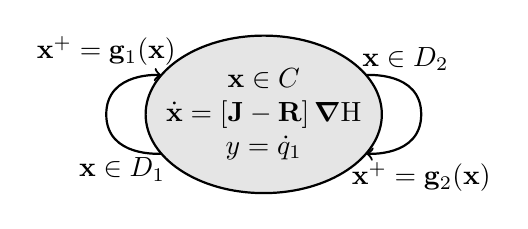
\begin{tikzpicture}
	%
	\fill[gray!20, draw = black,thick] (0,0) ellipse (1.5cm and 1cm);
	%	
	\draw (0,0) node[align = center](flow)  {$\xb\in\C$\\$\dot{\xb} = \left[\Jb-\Rb\right]\dH$\\$y = \dot{q}_1$};
	%
	\draw [thick,->] plot [smooth, tension=2] coordinates { (1.3,0.498888) (2,0) (1.3,-0.498888)};
	\draw [thick,->] plot [smooth, tension=2] coordinates { (-1.3,-0.498888) (-2,0) (-1.3,0.498888)};
	%
	\draw (1.8,0.7) node {$\xb\in\D_2$};
	\draw (2,-0.8) node {$\xb^+ = {\gb}_2(\xb)$};
	%
	%
	\draw (-1.8,-0.7) node {$\xb\in\D_1$};
	\draw (-2,0.8) node {$\xb^+ = {\gb}_1(\xb)$};
	%
\end{tikzpicture}
	\caption{Hybrid automata of the autonomous system. It has a single mode for flows, described by an autonomous port-Hamiltonian system, and it has two jumps: $\gb_1$ resets the states during  \textit{ball--ground} collisions ($\xb\in\D_1$) while $\gb_2$ resets the states during  \textit{robot-ball} collisions ($\xb\in\D_2$).}
	\label{fig:uHPH}
\end{figure}
%%%%%%%%%%%%%%%%%%%%%%%%%%%%%%%%%%%%%%%%%%%%%%%%%%%%%%%%%%%%%%%%%%%%%%%%%%%%%%%%%%%%%%%%%%%%%%%%%%%%%%%%%%%%%%%%%%%%%%%%%%%%%%%%%%%%%%%%%%%%%%%%%%%%%%%%%%%%%%%%%%%%%%%%%%%%%%%%%%%%%%%%%%
\newpage

\section{Analysis of the Autonomous Model}\label{sec:analysis_aut}
\subsection{Passivity and Autonomous Stability}
%
\begin{prop}
    The ball--dribbling robot is passive.
\end{prop}
%
\begin{proof}
    %
    Let $\hat{q}_1,~\hat{q}_2,~\hat{p}_1,~\hat{p}_2$ be the versors of the axes ${q}_1,~{q}_2,~{p}_1,~{p}_2$.
    %
    $\Ha(\xb)$ is nondecreasing along the eigendirections of $\gb_1$, $\gb_2$ which are, respectively, the one of the axis $(\hat{q}_1,\hat{q}_2,\hat{p}_1,\hat{p}_2)$ and $(\hat{q}_1, \hat{q}_2,m_2\hat{p}_1 + m_1\hat{p}_2,\hat{p}_1-\hat{p}_2)$, i.e. $\Ha$ is evenly diverging with respect to $\gb_1,~\gb_2$.
    %
    Thus, the ball--dribbling robot is passive for Proposition \ref{prop:pass_impulsive} as
    %
    $\Mb_1$ has eigenvalues $\lambda_{1,2,3} = 1$, $\lambda_4 = -c_g$ and $\Mb_2$ has eigenvalues $\lambda_{1,2,3} = 1$, $\lambda_4 = -c_i$, whose norms are indeed all less or equal than one.
    %
\end{proof}
%
Moreover, it very straightforward to prove that in the case of the autonomous system (u = 0), any neighborhood of the origin $\mymathbb{0}_4$ is a Lyapunov stable set.
%
\subsection{Chaotic Trajectories}
Let us consider the uncontrolled system and let set the physical parameters so that the system is conservative, i.e. $c_i = c_g = 1$, $\beta_1=\beta_2=0$. In this case, the Hamiltonian is constant in time,
%
\begin{equation}
    \forall t\geq 0 \quad \dot{\Ha}(\xb(t)) = 0
\end{equation}
%
In this case, trajectories happen on isolines of the Hamiltonian functions depending on the initial condition $\xb_0$:
%
\begin{equation}
    \forall t\geq 0 \quad \xb(t)\in\left\{\xb:\Ha(\xb) = \Ha(\x_0)\right\}
\end{equation}
%
and the volume of the phase--space is also conserved thanks to the Liuville theorem.
%

However, although the system is linear, it exhibits a chaotic behaviour due to its hybrid nature, with an exceptional sensitivity to the initial condition: trajectories starting ``very close'' tend to diverge in time (inside the limited phase--space).
%

This behaviour is shown by a numerical analysis performed through a Monte Carlo simulation integrating the system from 3000 initial conditions $\xb_0^i$ sampled by a multivariate normal distribution centered in a nominal initial condition $\xb_0$ and variance $\sigma = 10^{-6}$:
%
\begin{equation}
    \xb_0^i \sim \N(\xb_0,\sigma\mathbb{I}_n)
\end{equation}
%
Choosing $x_0\triangleq(2,1.5,0,0)$, $m_1 = 1\text{Kg}$, $m_2 = 0.15\text{Kg}$, the nominal trajectory (starting from $\xb_0$) and all the other 3000 ones have been integrated for $t = 20s$. The experiments have been carried out using Hybrid Equations (HyEQ) Toolbox \cite{sanfelice2013toolbox} for the MATLAB environment. The time evolution of the system's state in all the trials is shown in Fig. \ref{fig:chaos1}. The black trajectory is the nominal one (starting from $\xb_0$), where red dots and dashed blue lines indicate discrete events (impacts) and the value of the state after the events, respectively. Orange lines show the traces of all the other trajectories of the Monte Carlo runs (with initial condition sampled from $\N(\xb_0,\sigma\mathbb{I}_n)$). The blue dots at $t=0$ are the initial conditions. It can be noticed how trajectories, starting very close, diverge, densely covering the state--space.
%
\begin{figure}[!h]
    \centering
    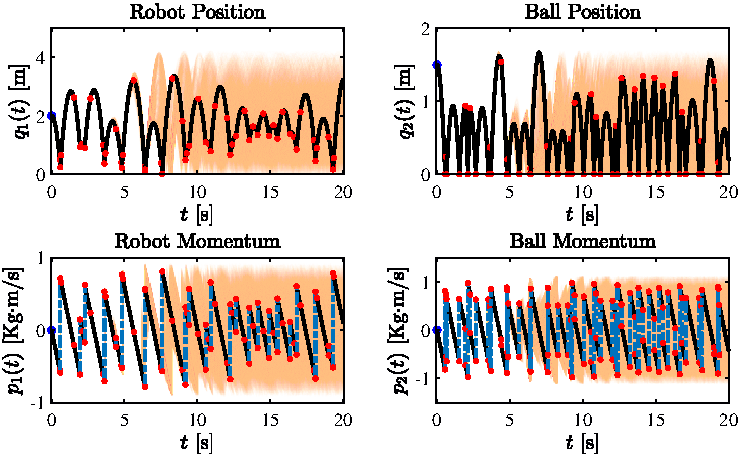
\includegraphics[width = \linewidth]{Figures/chaos1.pdf}
    \caption[Time evolution of the autonomous system' state in the Monte Carlo simulation]{Time evolution of the autonomous system' state in the Monte Carlo simulation. The black trajectory is the nominal one (starting from $\xb_0$), where red dots and dashed blue lines indicate discrete events (impacts) and the value of the state after the events, respectively. Orange lines show the traces of all the other trajectories of the Monte Carlo runs (with initial condition sampled from $\N(\xb_0,\sigma\mathbb{I}_n)$). The blue dots at $t=0$ are the initial conditions. It can be noticed how trajectories, starting very close, diverge, densely covering the state--space.}
    \label{fig:chaos1}
\end{figure}
%

This phenomenon is further emphasized by looking at the phase--space trajectories of the robot and the ball, respectively, represented in Fig. \ref{fig:chaos2}. The dashed black line is the nominal one (starting from $\xb_0$). Orange lines show the traces of all the other trajectories of the Monte Carlo runs (with initial condition sampled from $\N(\xb_0,\sigma\mathbb{I}_n)$). 
%
\begin{figure}[!h]
    \centering
    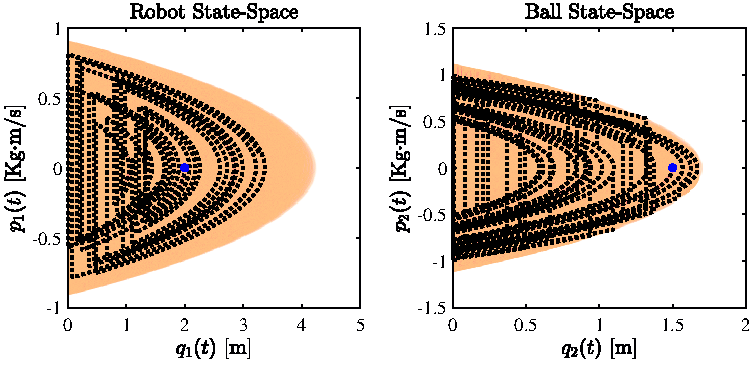
\includegraphics[width = \linewidth]{Figures/chaos2.pdf}
    \caption[Phase--space trajectory of the autonomous system in the Monte Carlo simulation]{Phase--space trajectory of the autonomous system in the Monte Carlo simulation. The dashed black line is the nominal one (starting from $\xb_0$). Orange lines show the traces of all the other trajectories of the Monte Carlo runs (with initial condition sampled from $\N(\xb_0,\sigma\mathbb{I}_n)$). The blue dots at are the initial conditions. It can be noticed how trajectories, starting very close, diverge, densely covering the state--space.}
    \label{fig:chaos2}
\end{figure}
%
\begin{figure}[!h]
    \centering
    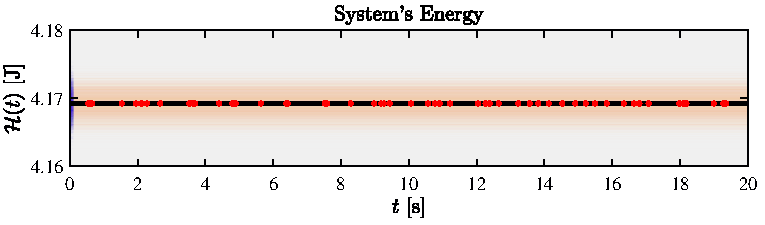
\includegraphics[width = \linewidth]{Figures/chaos3.pdf}
    \caption[Time evolution of the energy in the Monte Carlo simulation]{Time evolution of the energy in the Monte Carlo simulation. The black trajectory is the nominal one (starting from $\xb_0$), where red dots indicate discrete events (impacts). Orange lines show the traces of all the other trajectories of the Monte Carlo runs (with initial condition sampled from $\N(\xb_0,\sigma\mathbb{I}_n)$). The blue dots at $t=0$ are the initial energies of each Monte Carlo run. It can be noticed how, regardless the initial condition, energy is conserved in time.}
    \label{fig:chaos3}
\end{figure}

The time evolution of the energy (Hamiltonian function) among the Monte Carlo runs is also shown in Fig. \ref{fig:chaos3}. As expected, the energy is conserved trough time.
%

%
The experiment which has been done here numerically can be formalized as follows.
Instead of an initial condition, we considered an initial distribution (probability density) of the state $\psi(\xb_0)$ and we observed how this distribution evolved in time through the dynamics of the system, i.e. we approximated a solution of a partial differential equation of type
%
\begin{equation}
    \partial_t\psi(\xb) = \Gamma(\psi(\xb)).
\end{equation}
%
From the numerical Monte Carlo simulation, we build the histogram of the state at each value of the time are we built a phasegram plot representing the time evolution of state probability\footnote{i.e., the probability of finding the state of the system somewhere in the state--space.}, for each state of the system. It is reported in Figure \ref{fig:phasegram}. 
%
\begin{figure}[h]
    \centering
    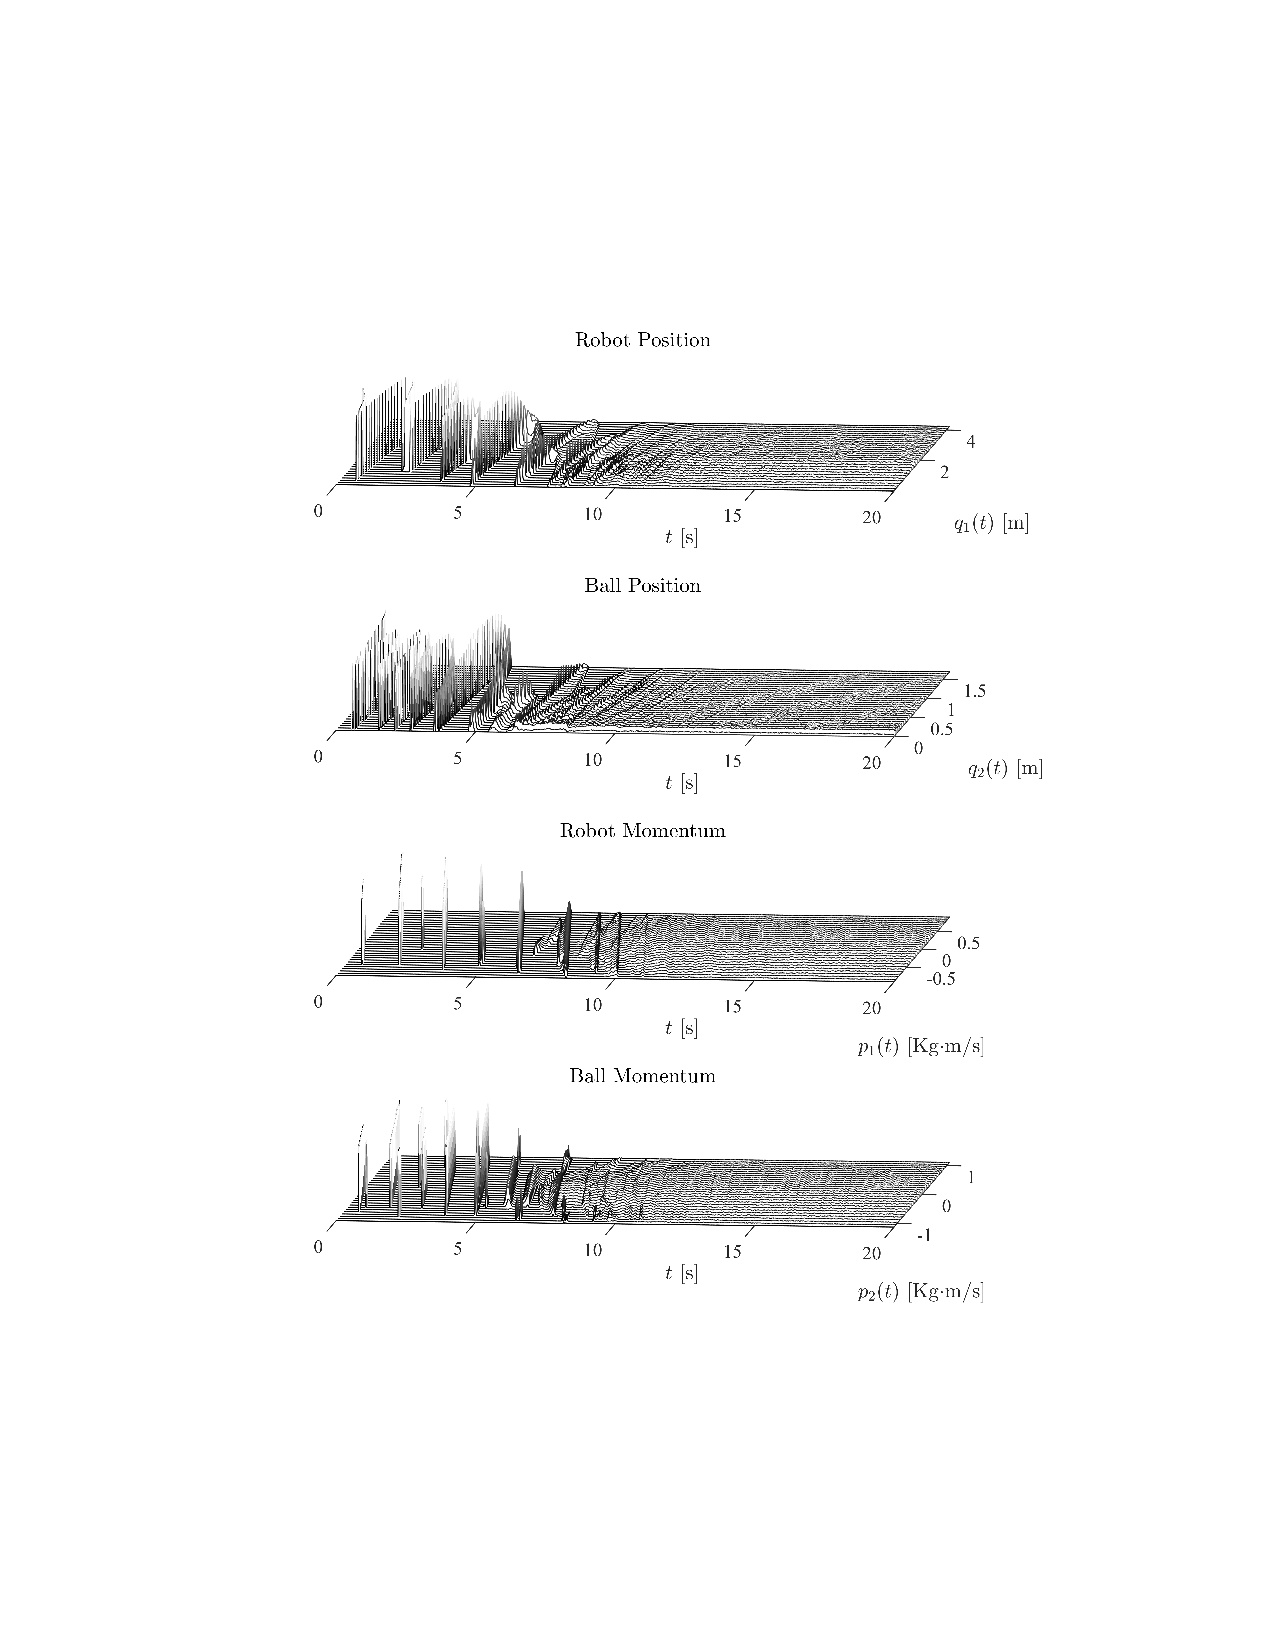
\includegraphics[width = 1\linewidth, trim={5cm 5.75cm 3.9cm 5.5cm},clip]{Figures/PhaseGram.pdf}
    \caption[Phasegram of the state probability function]{Phasegram of the state probability computed from the Monte Carlo Simulation. At $t=0$ the state probability is just a spike across the initial condition. Throughout time, the probability relaxes to with much larger variance.}
    \label{fig:phasegram}
\end{figure}
%
At $t=0$ the state probability is just a spike across the initial condition, i.e. $\N(\xb_0,\sigma\mathbb{I}_n)$. Throughout time, however the probability relaxes to with much larger variance. It means that, although all trajectories started very close one to the other, after a short period of time, the state might be everywhere in the state--space. Thus, the properties of the autonomous conservative ball--dribbling robot system resembles the ones of some stochastic system where the system has no ``memory'' of its past.
The same result is emphasized by looking the computed initial and final probability density functions $\psi_i$ and $\psi_f$ in Fig. \ref{fig:hist}.
%
\begin{figure}[h]
    \centering
    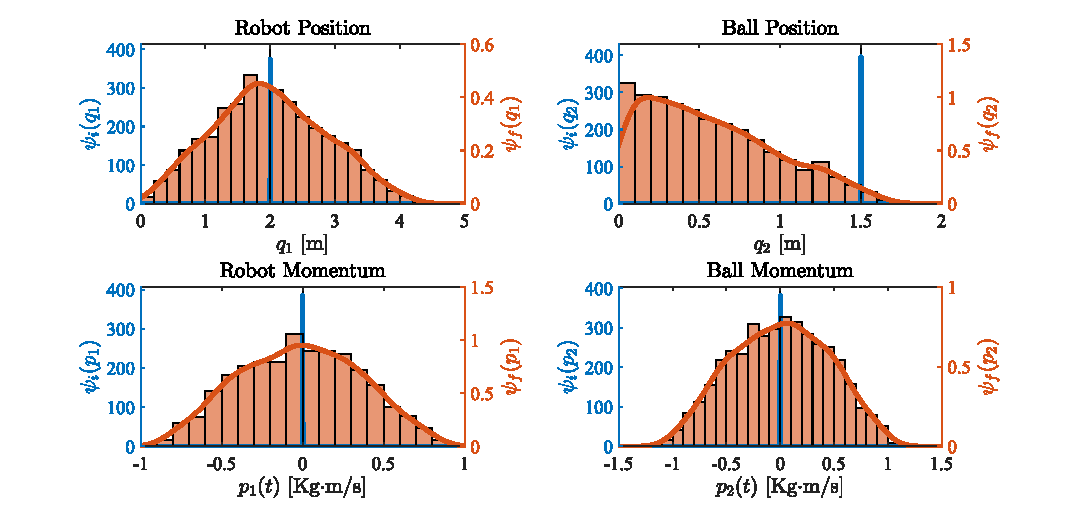
\includegraphics[width = 1\linewidth]{Figures/Hist.pdf}
    \caption{Histograms and reconstructed probability density functions of the state.}
    \label{fig:hist}
\end{figure}
%
\clearpage
%%%%%%%%%%%%%%%%%%%%%%%%%%%%%%%%%%%%%%%%%%%%%%%%%%%%%%%%%%%%%%%%%%%%%%%%
\section{Dribbling Control}\label{sec:control}
%
Let us consider the control task of continuously hitting the ball such that it reaches, at every cycle, the same maximum height $q_{2,max}^*$. In order to address this control problem, it is possible to design an hybrid controller with two modes, i.e., a \textit{wait mode} ($\Sa_{w}$) and a \textit{hit mode} ($\Sa_{h}$). In the wait state, the robot must stay at a constant height above the ball, to overcome any interference between its motion and the one of the ball and, at the same time, stay close enough to the ball to hit it quickly at the right time.
Then, in the hit state, the controller must move the robot toward the ball so that the exchanged impulse during the impact would lead the ball to come back to the desired peak $q_{2,max}^*$. In particular, the system would enter in the hit state whenever the ball reaches the peak of its bounce and switch back to the wait mode immediately after the impact between the two bodies. 
%
In both modes, we would like to exploit the passivity--based control theory. Besides, the system is under--actuated and the flows are decoupled. Therefore, it is impossible to shape the total energy of system setting its minimum in a desired configuration different from the origin. Although it is not possible to modify the energy of the ball, it is however possible to partially shape the Hamiltonian, i.e. the part relative to the robot. If 
%
\begin{equation}
    \Ha(\xb) = \Ha_1(q_1,p_1) + \Ha_2(q_2,p_2),
\end{equation}
%
it is possible to obtained a desired-shape Hamiltonian
%
\begin{equation}
     \Ha^*(\xb)  = \Ha_1^*(q_1,p_1) + \Ha_2(q_2,p_2)
\end{equation}
%
allowing to bring the robot in a desired configuration $q_1^*$. This might be achieved through an \textit{energy--balancing passivity--based controller}\footnote{In this case $q_1^*$ becomes a strict minimum of $\Ha_1^*$ and asymptotic stabilization must be achieved with $p_1 = 0$ at steady--state} \citep{ortega2001putting,ortega2008control,secchi2007control} described in Chapter \ref{chap:preliminaries}:
%
\begin{align*}
u &= \beta(\xb) + v = \beta(\xb) - k_dy \\
&= \frac{\partial V_1(q_1)}{\partial q_1} - k_p(q_1 -q_1^*) - k_d\dot{q}_1\\
&= \gamma m_1q_1- k_p(q_1 -q_1^*) - k_d\dot{q}_1
\end{align*}
%
As pointed out before, the controller has two separate modes and the control parameters $k_p$, $k_d$, $q_1^*$ should be changed during the state transitions.
% 
For this reason, let us collect the control parameters in a vector 
%
\begin{equation}
    \bm\omega = (k_p,k_d,q_1^*)
\end{equation}
%
and consider it as part of the state vector. The augmented model of the controlled system can be then rewritten as follows:
\begin{equation}\label{eq:HpHc}
    %
    \left\{ 
        \begin{matrix*}[l]\vspace{1pt}
            %
            \begin{bmatrix}\dot{\xb}\\\dot{\bm\omega}\end{bmatrix} = \begin{bmatrix}\left[\Jb-\Rb\right]{\dH^*(\xb)}+\Gb v(\x,\bm\omega)\\\mymathbb{0}_3\end{bmatrix} &(\xb,\bm\omega,v)\in\C\times\Omega\times\U\\
            %
            \begin{bmatrix}{\xb}^+\\{\bm\omega}^+\end{bmatrix} \in \G\times\Lambda&(\xb,\bm\omega)\in\D\times\Omega\\
            %
            y = \Gb^\top{\dH^*(\xb)}
        \end{matrix*}
    \right.
    %
\end{equation}
%
where $\Omega$ is the space of admissible parameters values and $\Lambda$ is the jump set--valued mapping of the control parameters. The shaped Hamiltonian $\Ha^*(\xb,\bm\omega)$, results to be
\[\Ha^*(\xb,\bm\omega) = \frac{1}{2}\pb^\top \Mb^{-1}\pb + \frac{1}{2}k_p(q_1 - q_1^*)^2+ \gamma m_2q_2\]
Notice that the choice of the control parameters influences both the closed-loop energy $\Ha^*$ (with $k_p$ and $q_1^*$) and the output feedback $v$ (with $k_d$).
%
Let us define a jump set $\D_3$ corresponding to the sub--manifold of the state--space where the ball reaches the peak $q_{2,max}$ of its bounce: $\D_3 = \left\{\xb:~p_2=0\right\}$.
It is clear that during the time evolution of the system, the state will cyclically enter in $\D_3$ and therefore the controller will periodically switch to $\Sa_h$ where the robot moves toward the ball until they collide, i.e. $\xb\in\D_2$, when the controller switches back to $\Sa_w$ where the robot waits above the ball at a distance $\delta$. The jumps maps resetting the control parameters are the following:
%
\begin{align*}
\bm\omega^+ = \bm\nu_{3}(\xb,\bm\omega) &=\begin{bmatrix}k_{p,h}&k_{d,h}&q_2\end{bmatrix}^\top &\quad&\xb\in\D_3\\
\bm\omega^+ = \bm\nu_{2}(\xb,\bm\omega) &=\begin{bmatrix}k_{p,w}&k_{d,w}&q_2 + \delta\end{bmatrix}^\top &\quad&\xb\in\D_2\\
\bm\omega^+ = \bm\nu_{1}(\xb,\bm\omega) &= \bm\omega &\quad&\xb\in\D_1
\end{align*}
%
Therefore,
%
\begin{equation}
    \Lambda \triangleq \left\{{\bm\nu}_i:\xb\in\D_i\Rightarrow \bm\omega^+ = \bm\nu_i(\bm\omega,\xb),~ i = 1,2,3\right\}.
\end{equation}
%
Figure \ref{fig:ctrl} shows the finite--state machine representing the controller.
When $\xb\in\D_3$, the state of the system does not jump, i.e. $\xb^+ = \gb_3(\xb)= \xb$ if $\xb\in\D_3$.
The set-valued mapping $\G$ is redefined considering $\gb_3$.
%
\begin{figure}[h]
	\centering
	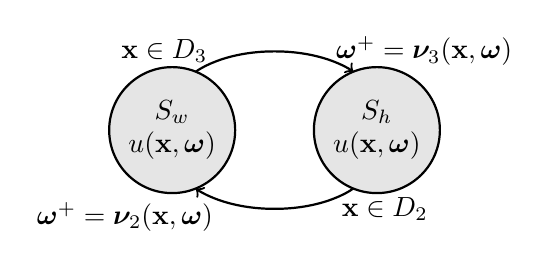
\begin{tikzpicture}
	%
	\fill[gray!20, draw = black,thick] (-1.3,0) circle (0.8cm);
	\fill[gray!20, draw = black,thick] (1.3,0) circle (0.8cm);
	%	
	\draw (-1.3,0) node[align = center](flow)  {$S_{w}$\\$u(\xb,\bm\omega)$};
	\draw (1.3,0) node[align = center](flow)  {$S_{h}$\\$u(\xb,\bm\omega)$};
	%
	\draw [thick,->] plot [smooth, tension=1.2] coordinates { (-1,0.74162) (0,1) (1,0.74162)};
	\draw [thick,->] plot [smooth, tension=1.2] coordinates { (1,-0.74162) (0,-1) (-1,-0.74162)};
	%
	\draw (1.9,1) node {$\bm\omega^+ = \bm\nu_{3}(\xb,\bm\omega)$};
	\draw (1.4,-1) node {$\xb\in\D_2$};
	%
	%
	\draw (-1.9,-1.1) node {$\bm\omega^+ = \bm\nu_{2}(\xb,\bm\omega)$};
	\draw (-1.4,1) node {$\xb\in\D_3$};
	%
	\end{tikzpicture}
	\caption{Finite state machine of the controller. It has an \textit{hit} state $\Sa_h$ in which it forces the robot to move toward the ball and a \textit{wait} state $\Sa_w$ in which it keeps the robot at a constant distance $\delta$ from the ball.The transitions happen as follows: $\Sa_h\rightarrow\Sa_w$ when the robot hits the ball, $\Sa_w\rightarrow\Sa_h$ when the ball reaches the peak of its bounce.}
	\label{fig:ctrl}
\end{figure}
%
\begin{rem}
    The behavior of the system strongly depends on the choice of the control parameters. Furthermore, unless a solution of (\ref{eq:HpHc}) is derived, it is not possible to find analytically two sets of control parameters (one for $S_{w}$ and one for $S_{h}$) which solve the control problem, i.e. ensuring that the ball bounces continuously reaching each time the desired peak $q_{2,max}^*$.
\end{rem}
 For the reasons stated in previous remark, a new paradigm of energy based control, which combines the traditional energy shaping approach with a basic form of {iterative learning control}: the \textit{iterative energy shaping}, has been introduced.
\begin{defn}[Iterative Energy Shaping Control]$\newline$
	First, let us define some further control parameters which are needed for the design.
	Let $\xi$ be a counter of the number of cycles of the system, i.e., the number of complete bounces of the ball. Let initialize $\xi$ to one. Let $e(\xi) = q_{2,max}^* - q_{2,max}$ computed when $\xb\in\D_3$ be the tracking error of the iterative energy shaping control loop. Thus, the control parameters vector can be redefined as 
	%
	\begin{equation}
	    \bm\omega \triangleq (k_p,k_d,q_1^*,\xi).
	\end{equation}
	%
	The iterative energy shaping control law is defined by means of the following control parameters jump maps:
	%
	\begin{align}
	&\bm\omega^+  \triangleq \bm\nu_{3}(\xb,\bm\omega)=\begin{bmatrix}k_0\varphi_\xi(e)&k_{d,h}&q_2&\xi+1\end{bmatrix}^\top &\xb\in\D_3\\
	&\bm\omega^+  \triangleq \bm\nu_{2}(\xb,\bm\omega)=\begin{bmatrix}k_{p,w}&k_{d,w}&q_2 + \delta&\xi\end{bmatrix}^\top &\xb\in\D_2
	\end{align}
	%
	where $\sigma>0$ is a constant scalar and $\varphi_\xi(e)$ is a scalar function of the error. When the controller is in the \textit{hit} state, the resulting shaped Hamiltonian assumes the following form:
	\begin{equation}
		\Ha^*(\xb,\bm\omega) = \frac{1}{2}\pb^\top \Mb^{-1}\pb + \frac{1}{2}k_0\varphi_\xi(e)(q_1 - q_1^*)^2+ \gamma m_2q_2
	\end{equation}
\end{defn}
%
A representation of the \textit{hybrid automata} corresponding to the final controlled system is pictured in Fig. \ref{fig:cHPH}.
%
\begin{figure}[h]
	%
	\centering
	%
	\scalebox{1}{
		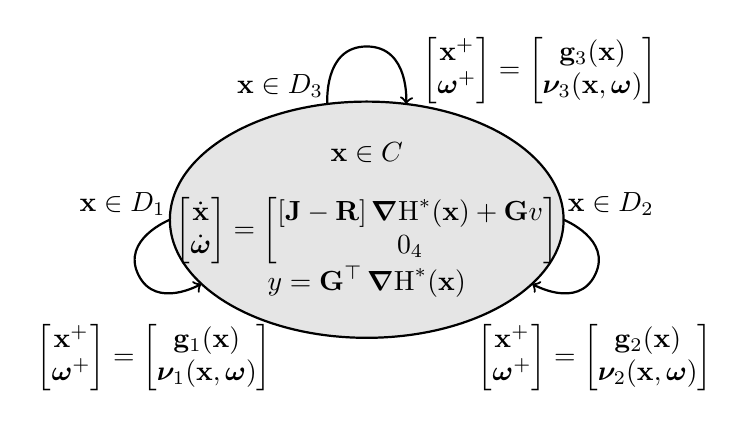
\begin{tikzpicture}
		% 
		\fill[gray!20, draw = black,thick] (0,0) ellipse (2.5cm and 1.5cm);
		%	
		\draw (0,0) node[align = center](flow)  {$\xb\in\C$\\\\$\begin{bmatrix}\dot{\xb}\\\dot{\bm\omega}\end{bmatrix} = \begin{bmatrix}\left[\Jb-\Rb\right]\dH^*(\xb)+\Gb v\\\mymathbb{0}_4\end{bmatrix}$\\$y = \Gb^\top\dH^*(\xb)$};
		%
		\draw [thick,->] plot [smooth, tension=2] coordinates { (-0.5,1.4697) (0,2.2) (0.5,1.4697)};
		\draw [thick,->] plot [smooth, tension=2] coordinates { (2.5,0) (2.9,-.7) (2.1,-0.8139)};
		\draw [thick,->] plot [smooth, tension=2] coordinates { (-2.5,0) (-2.9,-.7) (-2.1,-0.8139)};
		%
		\draw (3.1,0.2) node {$\xb\in\D_2$};
		\draw (2.9,-1.75) node[align = left] {$\begin{bmatrix}\xb^+\\\bm\omega^+\end{bmatrix} = \begin{bmatrix}\gb_2(\xb)\\\bm\nu_2(\xb,\bm\omega)\end{bmatrix}$};
		%
		\draw (-3.1,0.2) node {$\xb\in\D_1$};
		\draw (-2.7,-1.75) node[align = left] {$\begin{bmatrix}\xb^+\\\bm\omega^+\end{bmatrix} = \begin{bmatrix}\gb_1(\xb)\\\bm\nu_1(\xb,\bm\omega)\end{bmatrix}$};;
		%
		\draw (-1.1,1.7) node {$\xb\in\D_3$};
		\draw (2.2,1.9) node[align = left] {$\begin{bmatrix}\xb^+\\\bm\omega^+\end{bmatrix} = \begin{bmatrix}\gb_3(\xb)\\
		\bm\nu_3(\xb,\bm\omega)\end{bmatrix}$};
		%
		\end{tikzpicture}
	}
	\caption[Hybrid automata representing the controlled system]{Hybrid automata representing the controlled system. Although the \textit{iterative energy shaping} controller has two modes, the controlled system is still an impulsive port--Hamiltonian system}
	\label{fig:cHPH}
\end{figure}
%
The main idea is to iteratively adjust the slope (steepness) of the energy of the system as function of the error. For instance, when $e>0$, it can be derived that the robot had hit the ball with not enough momentum. Thus, at the next cycle, the energy function should be steeper so that the robot will accelerate faster toward the ball, since the dissipation rate $k_d$ of the damping injection didn't change. The same concept can be adopted for $e<0$, by making the the energy function less steep.
%
A possible choice of $\varphi_\xi(e)$ is
%
\begin{equation}
    \varphi_\xi(e)  \triangleq \varphi_0 + a\cdot e(\xi) + b\cdot\sum_{i = 1}^{\xi}e(i)
\end{equation}
%
which provides a proportional and integral action with a constant offset $\varphi_0$ in response to the error. The integral action should ensure zero steady state error.
%
\section{Numerical Simulations}
%
To validate the proposed control scheme, numerical simulations have been performed. The physical parameters of the system have been chosen as $m_1 = 0.1\text{Kg}$, $m_2 = 0.05\text{Kg}$, $\beta_1 = 0.2\text{N}\cdot \text{s}/\text{m}$, $\beta_2 = 0.3\text{N}\cdot \text{s}/\text{m}$, $c_g = c_i = 0.8$. The initial conditions have been set to $q_1(0) = 2$m, $q_2(0) = 1.5$m, $p_1(0) = p_2(0) = 0\text{Kg}\cdot \text{m}/\text{s}$. Note that the mass of the ball $m_2$ has been chosen similar to the one of a standard golf ball ($\approx 46g$).
%%%%%%%%%%%%%%%%%%%%%%%%%%%%%
\subsection{Autonomous System}
%
Firstly, the behavior of the uncontrolled system has been simulated. The time evolution of the state variables are shown in Fig. \ref{fig:aut1}.
%
\begin{figure}[h]
	\centering
	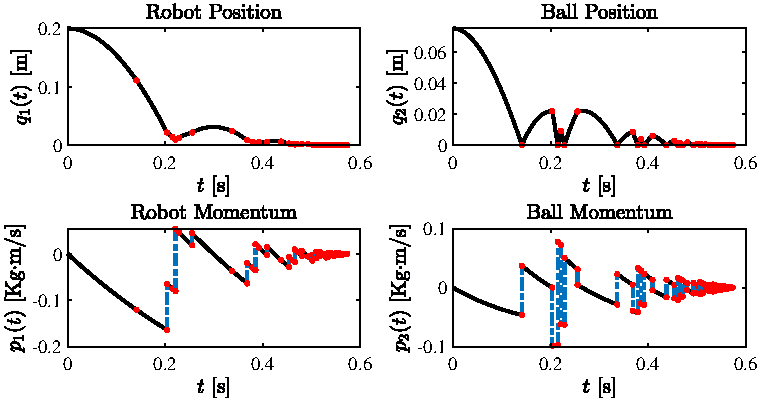
\includegraphics[width = \linewidth]{Figures/aut1.pdf}
	\caption[Uncontrolled system: time evolution of the robot and ball position states]{Uncontrolled system: time evolution of the robot and ball position states (position and momentum). Red dots correspond to system's jumps while dashed blue lines highlight discontinuous state changes. Notice that both the position and velocity goes asymptotically to zero.}
	\label{fig:aut1}
\end{figure}
%
The phase--space trajectory of the autonomous system is also represented in Fig. \ref{fig:aut2} over the energy of the system. 
%
\begin{figure}[h]
	\centering
    %\definecolor{ocean}{rgb}{0.00000,0.44700,0.74100}
\definecolor{mycolor1}{rgb}{0.00000,0.44700,0.74100}%

\begin{tikzpicture}
\begin{axis}[
width=5cm,
height=5cm,
at={(1in,0.331in)},
view={0}{90},
colorbar horizontal,
colormap = {whiteblack}{color(0cm)  = (white);color(1cm) = (black)},
colorbar style = {at = {(0,-0.25)}},
xmin=0,
xmax=.2,
xlabel style={font=\color{white!15!black},at = {(0.75in,-0.125in)}},
xlabel={$q_1(t)~[m]$},
ymin=-.2,
ymax=.1,
ylabel style={font=\color{white!15!black},at = {(-0.1in,0.75in)}},
ylabel={$p_1(t)~$[Kg$\cdot$m/s]},
title = {robot phase--space},
axis background/.style={fill=white},
]
\addplot3[contour filled={number = 25,labels={false}},mesh/rows=25,mesh/cols=25,mesh/check=false,forget plot
] table {H1_a.dat};
%%%%%%%%%%%%%%%%%%%%%%%%%%%%%%%%%%%%
\addplot [color=black, line width=1.5pt]
  table[row sep=crcr]{%
0.2	0\\
0.2	0\\
0.199999967381998	-7.99934763995355e-05\\
0.199998826071083	-0.000479765214216573\\
0.199989131483394	-0.00145882629667888\\
0.199969656068965	-0.00243593121379302\\
0.1999404193699	-0.00341108387397995\\
0.199901440889258	-0.00438428817785163\\
0.199852740091133	-0.00535554801822656\\
0.199794336400727	-0.00632486728014541\\
0.199726249204433	-0.00729224984088653\\
0.199648497849907	-0.00825769956998144\\
0.199561101646152	-0.00922122032923035\\
0.199464079863588	-0.0101828159727176\\
0.199357451734135	-0.011142490346827\\
0.199241236451287	-0.0121002472902574\\
0.199115453170189	-0.0130560906340378\\
0.198980121007714	-0.0140100242015429\\
0.198835259042541	-0.0149620518085082\\
0.198680886315227	-0.0159121772630453\\
0.198517021828288	-0.0168604043656575\\
0.198343684546272	-0.0178067369092544\\
0.198160893395837	-0.0187511786791674\\
0.197968667265824	-0.0196937334531649\\
0.197767025007336	-0.0206344050014671\\
0.197555985433808	-0.0215731970867617\\
0.19733556732109	-0.0225101134642181\\
0.197105789407515	-0.0234451578815031\\
0.196866670393978	-0.0243783340787956\\
0.196618228944009	-0.0253096457888017\\
0.196360483683848	-0.0262390967367695\\
0.19609345320252	-0.027166690640504\\
0.19581715605191	-0.028092431210382\\
0.195531610746835	-0.0290163221493671\\
0.195236835765121	-0.0299383671530242\\
0.194932849547673	-0.0308585699095347\\
0.194619670498553	-0.0317769340997106\\
0.194297316985051	-0.0326934633970102\\
0.193965807337758	-0.0336081614675517\\
0.193625159850643	-0.0345210319701286\\
0.193275392781121	-0.0354320785562243\\
0.192916524350131	-0.0363413048700261\\
0.192548572742204	-0.0372487145484408\\
0.19217155610554	-0.038154311221108\\
0.191785492552079	-0.0390580985104158\\
0.191390400157573	-0.0399600800315146\\
0.190986296961657	-0.0408602593923315\\
0.190573200967926	-0.0417586401935853\\
0.190151130144001	-0.0426552260288003\\
0.189720102421606	-0.0435500204843211\\
0.189280135696634	-0.0444430271393267\\
0.188831247829225	-0.045334249565845\\
0.188373456643834	-0.0462236913287668\\
0.187906779929302	-0.0471113559858603\\
0.187431235438927	-0.0479972470877854\\
0.186946840890538	-0.0488813681781077\\
0.186453613966563	-0.0497637227933127\\
0.1859515723141	-0.05064431446282\\
0.185440733544988	-0.0515231467089975\\
0.184921115235877	-0.0524002230471754\\
0.184392734928301	-0.0532755469856602\\
0.183855610128744	-0.0541491220257488\\
0.183309758308713	-0.0550209516617425\\
0.182755196904805	-0.0558910393809611\\
0.182191943318783	-0.0567593886637566\\
0.181620014917636	-0.0576260029835272\\
0.181039429033657	-0.0584908858067314\\
0.180450202964509	-0.0593540405929017\\
0.179852353973292	-0.0602154707946584\\
0.179245899288617	-0.0610751798577234\\
0.17863085610467	-0.0619331712209341\\
0.178007241581285	-0.0627894483162571\\
0.17737507284401	-0.0636440145688019\\
0.176734366984174	-0.0644968733968348\\
0.17608514105896	-0.0653480282117921\\
0.175427412091471	-0.0661974824182942\\
0.174761197070796	-0.0670452394141591\\
0.17408651295208	-0.067891302590416\\
0.173403376656593	-0.0687356753313186\\
0.172711805071795	-0.0695783610143591\\
0.172011815051406	-0.0704193630102812\\
0.171303423415471	-0.0712586846830942\\
0.170586646950429	-0.0720963293900858\\
0.16986150240918	-0.072932300481836\\
0.169128006511151	-0.0737666013022302\\
0.168386175942364	-0.0745992351884729\\
0.167636027355503	-0.0754302054711006\\
0.166877577369979	-0.0762595154739958\\
0.166110842571997	-0.0770871685143994\\
0.165335839514624	-0.0779131679029247\\
0.164552584717852	-0.0787375169435705\\
0.163761094668669	-0.0795602189337339\\
0.16296138582112	-0.080381277164224\\
0.162153474596374	-0.0812006949192748\\
0.161337377382792	-0.0820184754765585\\
0.160513110535992	-0.0828346221071984\\
0.15968069037891	-0.083649138075782\\
0.158840133201872	-0.0844620266403744\\
0.157991455262655	-0.0852732910525309\\
0.157134672786551	-0.0860829345573103\\
0.156269801966437	-0.0868909603932875\\
0.155396858962835	-0.0876973717925671\\
0.154515859903979	-0.0885021719807957\\
0.153626820885876	-0.0893053641771752\\
0.152729757972377	-0.0901069515944754\\
0.151824687195235	-0.090906937439047\\
0.150911624554173	-0.0917053249108346\\
0.149990586016945	-0.092502117203389\\
0.149061587519402	-0.0932973175038804\\
0.148124644965556	-0.0940909289931113\\
0.147179774227642	-0.0948829548455284\\
0.146226991146182	-0.0956733982292365\\
0.145266311530049	-0.0964622623060099\\
0.144297751156531	-0.0972495502313062\\
0.14332132577139	-0.0980352651542779\\
0.14233705108893	-0.098819410217786\\
0.141344942792058	-0.0996019885584117\\
0.140345016532346	-0.100383003306469\\
0.139337287930095	-0.101162457586019\\
0.138321772574394	-0.101940354514879\\
0.137298486023188	-0.102716697204638\\
0.136267443803336	-0.103491488760667\\
0.135228661410673	-0.104264732282135\\
0.134182154310077	-0.105036430862015\\
0.133127937935522	-0.105806587587104\\
0.13206602769015	-0.10657520553803\\
0.130996438946323	-0.107342287789265\\
0.129919187045693	-0.108107837409139\\
0.128834287299257	-0.108871857459852\\
0.127741754987421	-0.109634350997484\\
0.12664160536006	-0.110395321072012\\
0.125533853636582	-0.111154770727317\\
0.124418515005985	-0.111912703001197\\
0.123295604626918	-0.112669120925384\\
0.122165137627746	-0.113424027525549\\
0.121027129106605	-0.114177425821321\\
0.119881594131468	-0.114929318826294\\
0.118728547740197	-0.11567970954804\\
0.117568004940614	-0.116428600988123\\
0.116399980710552	-0.117175996142111\\
0.115224489997919	-0.117921897999584\\
0.114041547720758	-0.118666309544152\\
0.112851168767303	-0.119409233753461\\
0.111653367996044	-0.120150673599209\\
0.111003126035683	-0.120550649027536\\
};

\addplot [color=black, line width=1.5pt]
  table[row sep=crcr]{%
0.111003126035683	-0.120550649027536\\
0.111003126035683	-0.120550649027536\\
0.110873945268924	-0.120629901224444\\
0.110226768466994	-0.121025907615357\\
0.109012817113077	-0.121764117344574\\
0.107791491039044	-0.122500852129767\\
0.106562804979595	-0.123236114917877\\
0.105326773639992	-0.123969908649957\\
0.104083411696113	-0.124702236261181\\
0.102832733794515	-0.125433100680861\\
0.101574754552493	-0.126162504832457\\
0.100309488558133	-0.126890451633585\\
0.0990369503703772	-0.127616943996034\\
0.0977571545190772	-0.128341984825774\\
0.0964701155050545	-0.129065577022969\\
0.0951758478001579	-0.12978772348199\\
0.0938743658473213	-0.130508427091422\\
0.0925656840606218	-0.131227690734083\\
0.0912498168253371	-0.131945517287026\\
0.0899267784980029	-0.132661909621559\\
0.0885965834064708	-0.133376870603252\\
0.0872592458499652	-0.134090403091951\\
0.0859147800991405	-0.134802509941786\\
0.0845632003961387	-0.135513194001186\\
0.0832045209546456	-0.136222458112887\\
0.0818387559599481	-0.136930305113948\\
0.0804659195689911	-0.137636737835756\\
0.0790860259104336	-0.138341759104045\\
0.0776990890847058	-0.139045371738899\\
0.076305123164065	-0.139747578554771\\
0.0749041421926524	-0.140448382360489\\
0.0734961601865485	-0.141147785959268\\
0.0720811911338302	-0.141845792148724\\
0.0706592489946258	-0.142542403720883\\
0.0692303477011715	-0.143237623462193\\
0.0677945011578667	-0.143931454153532\\
0.0663517232413299	-0.144623898570224\\
0.0649020278004541	-0.145314959482049\\
0.063445428656462	-0.146004639653251\\
0.0619819396029617	-0.146692941842551\\
0.0605115744060017	-0.147379868803159\\
0.0590343468041257	-0.148065423282783\\
0.0575502705084279	-0.148749608023644\\
0.0560593592026076	-0.14943242576248\\
0.0545616265430243	-0.150113879230563\\
0.0530570861587518	-0.150793971153709\\
0.0515457516516331	-0.151472704252285\\
0.0500276365963347	-0.152150081241225\\
0.048502754540401	-0.152826104830038\\
0.0469711190043082	-0.15350077772282\\
0.0454327434815187	-0.154174102618262\\
0.0438876414385349	-0.154846082209665\\
0.0423358263149532	-0.155516719184949\\
0.0407773115235174	-0.156186016226662\\
0.0392121104501729	-0.156853976011993\\
0.03764023645412	-0.157520601212782\\
0.0360617028678669	-0.158185894495532\\
0.0344765229972839	-0.158849858521415\\
0.0328847101216559	-0.159512495946289\\
0.0312862774937359	-0.160173809420705\\
0.0296812383397976	-0.160833801589918\\
0.028069605859689	-0.161492475093896\\
0.0264513932268845	-0.162149832567335\\
0.0248266135885379	-0.162805876639666\\
0.0231952800655351	-0.163460609935065\\
0.0219480095000046	-0.163958559802086\\
};
%\addlegendentry{data2}

\addplot [color=mycolor1, dashdotted, line width=1pt, mark size=0.5pt, mark=*, mark options={solid, fill=red, red}]
  table[row sep=crcr]{%
0.111003126035683	-0.120550649027536\\
0.111003126035683	-0.120550649027536\\
};
%\addlegendentry{data3}

\addplot [color=black, line width=1.5pt]
  table[row sep=crcr]{%
0.0219480096000046	-0.065408056320056\\
0.0219480096000046	-0.065408056320056\\
0.0213610862698025	-0.0661658766261791\\
0.0206951869912011	-0.0670136967704588\\
0.0200208179837062	-0.0678598229689598\\
0.0193379961698475	-0.0687042586061881\\
0.0186467384383433	-0.0695470070598872\\
0.0179470616441683	-0.0703880717010522\\
0.017238982608621	-0.0712274558939427\\
0.0165225181193908	-0.0720651629960967\\
0.0157976849306254	-0.0729011963583436\\
0.0150644997629975	-0.0737355593248181\\
0.0143229793037722	-0.074568255232973\\
0.0140822597838371	-0.0748362274183675\\
};
%\addlegendentry{data4}

\addplot [color=mycolor1, dashdotted, line width=1pt, mark size=0.5pt, mark=*, mark options={solid, fill=red, red}]
  table[row sep=crcr]{%
0.0219480095000046	-0.163958559802086\\
0.0219480096000046	-0.065408056320056\\
};
%\addlegendentry{data5}

\addplot [color=black, line width=1.5pt]
  table[row sep=crcr]{%
0.0140822597838371	-0.0748362274183675\\
0.0140822597838371	-0.0748362274183675\\
0.014043800523677	-0.0748789359842696\\
0.0138511751519139	-0.0750924129995873\\
0.013096099715432	-0.0759223979122909\\
0.0123327327241388	-0.0767507245140323\\
0.0115610907445722	-0.077577396118119\\
0.0107811903101695	-0.0784024160312385\\
0.00999304792133467	-0.0792257875534715\\
0.00928590400525915	-0.0799559502607498\\
};
%\addlegendentry{data6}

\addplot [color=mycolor1, dashdotted, line width=1pt, mark size=0.5pt, mark=*, mark options={solid, fill=red, red}]
  table[row sep=crcr]{%
0.0140822597838371	-0.0748362274183675\\
0.0140822597838371	-0.0748362274183675\\
};
%\addlegendentry{data7}

\addplot [color=black, line width=1.5pt]
  table[row sep=crcr]{%
0.00928590410525915	0.0544550947842129\\
0.00928590410525915	0.0544550947842129\\
0.00960822168881119	0.0538065018345354\\
0.0101408472708482	0.0527189767181279\\
0.0106626084697222	0.0516336244783532\\
0.0111735269924851	0.0505504407738006\\
0.0116736245028183	0.0494694212717339\\
0.012162922621119	0.0483905616480738\\
0.012641442924587	0.0473138575873802\\
0.0130153166228394	0.0464568105343072\\
};
%\addlegendentry{data8}

\addplot [color=mycolor1, dashdotted, line width=1pt, mark size=0.5pt, mark=*, mark options={solid, fill=red, red}]
  table[row sep=crcr]{%
0.00928590400525915	-0.0799559502607498\\
0.00928590410525915	0.0544550947842129\\
};
%\addlegendentry{data9}

\addplot [color=black, line width=1.5pt]
  table[row sep=crcr]{%
0.0130153166228394	0.0464568105343072\\
0.0130153166228394	0.0464568105343072\\
0.0130520250736697	0.0463718829387801\\
0.0132345600994249	0.0459474464068239\\
0.0136886736653454	0.0448756236936398\\
0.0141320797152157	0.0438059424836657\\
0.0145647996426671	0.0427383984981754\\
0.0149868547985866	0.0416729874669916\\
0.0153982664912017	0.0406097051284685\\
0.0157990559861665	0.0395485472294756\\
0.0161892445066459	0.0384895095253797\\
0.0165688532334012	0.0374325877800286\\
0.0169379033048743	0.036377777765734\\
0.0172964158172725	0.0353250752632544\\
0.0176444118246529	0.0342744760617783\\
0.0179819123390066	0.0332259759589075\\
0.0183089383303426	0.0321795707606403\\
0.0186255107267718	0.0311352562813545\\
0.0189316504145909	0.0300930283437907\\
0.0192273782383656	0.0290528827790357\\
0.019512715001014	0.028014815426506\\
0.0197876814638903	0.0269788221339308\\
0.0200522983468671	0.0259448987573354\\
0.0203065863284188	0.0249130411610251\\
0.0205505660457044	0.023883245217568\\
0.0207842580946495	0.0228555068077789\\
0.0210076830300293	0.021829821820703\\
0.0212208613655503	0.0208061861535988\\
0.0214238135739326	0.0197845957119223\\
0.021616560086992	0.0187650464093104\\
0.0216673234911117	0.018487535439195\\
};
%\addlegendentry{data10}

\addplot [color=mycolor1, dashdotted, line width=1pt, mark size=0.5pt, mark=*, mark options={solid, fill=red, red}]
  table[row sep=crcr]{%
0.0130153166228394	0.0464568105343072\\
0.0130153166228394	0.0464568105343072\\
};
%\addlegendentry{data11}

\addplot [color=black, line width=1.5pt]
  table[row sep=crcr]{%
0.0216673235911117	0.0445428893967084\\
0.0216673235911117	0.0445428893967084\\
0.0220002095780532	0.0437364747396123\\
0.0224322355222784	0.0426690695507672\\
0.0228535980815511	0.0416037970389127\\
0.0232643185613285	0.0405406529429573\\
0.0236644182244996	0.039479633010323\\
0.0240539182914703	0.0384207329969289\\
0.0244328399402478	0.0373639486671734\\
0.0248012043065259	0.0363092757939178\\
0.025159032483769	0.0352567101584692\\
0.0255063455232968	0.0342062475505636\\
0.0258431644343686	0.0331578837683492\\
0.026169510184267	0.0321116146183695\\
0.0264854036983819	0.0310674359155466\\
0.0267908658602945	0.030025343483164\\
0.0270859175118602	0.0289853331528509\\
0.0273705794532927	0.0279474007645644\\
0.0276448724432468	0.0269115421665736\\
0.0279088171989011	0.0258777532154427\\
0.0281624343960417	0.0248460297760146\\
0.0284057446691443	0.0238163677213941\\
0.0286387686114568	0.0227887629329316\\
0.0288615267750819	0.0217632113002066\\
0.029074039671059	0.0207397087210111\\
0.0292763277694467	0.0197182511013336\\
0.029468411499404	0.0186988343553421\\
0.0296503112492728	0.0176814544053684\\
0.0298220473666587	0.0166661071818912\\
0.0299836401585132	0.0156527886235203\\
0.0301351098912141	0.0146414946769801\\
0.0302764767906471	0.0136322212970935\\
0.0304077610422866	0.0126249644467656\\
0.0305289827912762	0.0116197200969677\\
0.0306401621425097	0.010616484226721\\
0.0307413191607112	0.00961525282308071\\
0.0308324738705154	0.00861602188111986\\
0.030913646256548	0.00761878740391335\\
0.030984856263505	0.00662354540252195\\
0.0310461237962332	0.00563029189597632\\
0.0310974687198092	0.0046390229112611\\
0.0311389108596196	0.00364973448329904\\
0.0311704700014393	0.00266242265493509\\
0.0311921658915116	0.00167708347692064\\
0.0312040182366266	0.000693713007897637\\
0.0312060467042002	-0.000287692685617093\\
0.0311982709223529	-0.00126713752924764\\
0.0311807104799882	-0.00224462544077469\\
0.0311533849268707	-0.00322016033015118\\
0.0311163137737047	-0.004193746099518\\
0.0310695164922122	-0.0051653866432195\\
0.0310130125152106	-0.00613508584781916\\
0.0309468212366903	-0.00710284759211511\\
0.0308709620118927	-0.0080686757471556\\
0.0307854541573875	-0.00903257417625454\\
0.0306903169511495	-0.00999454673500695\\
0.0305855696326365	-0.0109545972713043\\
0.0304712314028655	-0.0119127296253502\\
0.0303473214244901	-0.0128689476296751\\
0.0302138588218766	-0.0138232551091524\\
0.0300708626811812	-0.0147756558810133\\
0.0299183520504255	-0.0157261537548621\\
0.0297563459395734	-0.0166747525326917\\
0.0295848633206068	-0.0176214560088984\\
0.0294039231276015	-0.0185662679702974\\
0.0292135442568031	-0.0195091921961377\\
0.0290137455667024	-0.0204502324581175\\
0.0288045458781109	-0.0213893925203992\\
0.0285859639742362	-0.0223266761396243\\
0.0283580186007568	-0.0232620870649284\\
0.0281207284658976	-0.0241956290379566\\
0.0278741122405042	-0.0251273057928779\\
0.027618188558118	-0.0260571210564007\\
0.0273529760150504	-0.0269850785477871\\
0.0270784931704575	-0.0279111819788686\\
0.0267947585464141	-0.0288354350540599\\
0.0265017906279878	-0.0297578414703746\\
0.0261996078633131	-0.0306784049174397\\
0.0258882286636652	-0.0315971290775101\\
0.0255676714035334	-0.0325140176254837\\
0.0252379544206947	-0.033429074228916\\
0.0248990960162873	-0.0343423025480345\\
0.0245511144548837	-0.0352537062357538\\
0.024206561480461	-0.03613178120804\\
};
%\addlegendentry{data12}

\addplot [color=mycolor1, dashdotted, line width=1pt, mark size=0.5pt, mark=*, mark options={solid, fill=red, red}]
  table[row sep=crcr]{%
0.0216673234911117	0.018487535439195\\
0.0216673235911117	0.0445428893967084\\
};
%\addlegendentry{data13}

\addplot [color=black, line width=1.5pt]
  table[row sep=crcr]{%
0.024206561480461	-0.03613178120804\\
0.024206561480461	-0.03613178120804\\
0.0241434365718622	-0.0362901693707391\\
0.0238236730155906	-0.0370812823815791\\
0.0234483290273901	-0.037987213583939\\
0.0230639347804385	-0.0388913347345487\\
0.0226705083571647	-0.0397936494498939\\
0.0222680678038693	-0.0406941613392348\\
0.0218566311307959	-0.0415928740046201\\
0.021436216312204	-0.0424897910409018\\
0.0210068412864401	-0.043384916035749\\
0.0205685239560102	-0.044278252569663\\
0.0201212821876509	-0.0451698042159911\\
0.0196651338124011	-0.0460595745409412\\
0.0192000966256733	-0.0469475671035956\\
0.0187261883873246	-0.0478337854559259\\
0.018243426821728	-0.0487182331428066\\
0.0177518296178431	-0.0496009137020296\\
0.0172514144292871	-0.0504818306643184\\
0.016742198874405	-0.051360987553342\\
0.0162242005363405	-0.0522383878857291\\
0.0156974369631062	-0.0531140351710822\\
0.0151619256676535	-0.0539879329119917\\
0.0146176841279432	-0.0548600846040496\\
0.0140647297870148	-0.0557304937358639\\
0.0135030800530569	-0.0565991637890723\\
0.0129327522994763	-0.0574660982383562\\
0.0123537638649678	-0.0583313005514545\\
0.0117661320535834	-0.0591947741891777\\
0.0111698741348017	-0.0600565226054213\\
0.0105650073435967	-0.0609165492471803\\
0.00995154888050709	-0.0617748575545624\\
0.00932951591170463	-0.0626314509608019\\
0.00869892556906321	-0.0634863328922736\\
0.00857212106226058	-0.0636566496567663\\
};
%\addlegendentry{data14}

\addplot [color=mycolor1, dashdotted, line width=1pt, mark size=0.5pt, mark=*, mark options={solid, fill=red, red}]
  table[row sep=crcr]{%
0.024206561480461	-0.03613178120804\\
0.024206561480461	-0.03613178120804\\
};
%\addlegendentry{data15}

\addplot [color=black, line width=1.5pt]
  table[row sep=crcr]{%
0.00857212116226058	-0.0194049517610908\\
0.00857212116226058	-0.0194049517610908\\
0.00839879882932497	-0.0202282951193367\\
0.00819181629622749	-0.0211678986127172\\
0.00797544711796713	-0.0221056247770652\\
0.00774971004907341	-0.0230414773632864\\
0.00751462380660433	-0.0239754601147926\\
0.00727020707022115	-0.024907576767516\\
0.00701647848226316	-0.0258378310499244\\
0.00675345664782221	-0.0267662266830362\\
0.00648116013481716	-0.0276927673804352\\
0.00619960747406817	-0.0286174568482854\\
0.0059965560509815	-0.0292651122340497\\
};
%\addlegendentry{data16}

\addplot [color=mycolor1, dashdotted, line width=1pt, mark size=0.5pt, mark=*, mark options={solid, fill=red, red}]
  table[row sep=crcr]{%
0.00857212106226058	-0.0636566496567663\\
0.00857212116226058	-0.0194049517610908\\
};
%\addlegendentry{data17}

\addplot [color=black, line width=1.5pt]
  table[row sep=crcr]{%
0.0059965560509815	-0.0292651122340497\\
0.0059965560509815	-0.0292651122340497\\
0.00596150042181735	-0.0293753905855554\\
0.00578424539213988	-0.0299263869663126\\
0.00548037885683717	-0.030846613659252\\
0.00516731925073715	-0.031765001738032\\
0.00484508494160753	-0.0326815548762061\\
0.0045136942605172	-0.033596276739988\\
0.00417316550190955	-0.0345091709882665\\
0.00396077363772996	-0.0350656338020219\\
};
%\addlegendentry{data18}

\addplot [color=mycolor1, dashdotted, line width=1pt, mark size=0.5pt, mark=*, mark options={solid, fill=red, red}]
  table[row sep=crcr]{%
0.0059965560509815	-0.0292651122340497\\
0.0059965560509815	-0.0292651122340497\\
};
%\addlegendentry{data19}

\addplot [color=black, line width=1.5pt]
  table[row sep=crcr]{%
0.00396077373772996	0.0209700851431617\\
0.00396077373772996	0.0209700851431617\\
0.00408263075107509	0.0203673416367906\\
0.0042811988998089	0.0193466280070438\\
0.00446957011257679	0.0183279537644902\\
0.0046477647628704	0.0173113148344315\\
0.00481580318347514	0.0162967071503105\\
0.00497370566655146	0.0152841266536953\\
0.00512149246371605	0.0142735692942624\\
0.0051886124074337	0.0137909054927752\\
};
%\addlegendentry{data20}

\addplot [color=mycolor1, dashdotted, line width=1pt, mark size=0.5pt, mark=*, mark options={solid, fill=red, red}]
  table[row sep=crcr]{%
0.00396077363772996	-0.0350656338020219\\
0.00396077373772996	0.0209700851431617\\
};
%\addlegendentry{data21}

\addplot [color=black, line width=1.5pt]
  table[row sep=crcr]{%
0.0051886124074337	0.0137909054927752\\
0.0051886124074337	0.0137909054927752\\
0.00521211858182868	0.0136179405861344\\
0.0053252021435366	0.012754005514984\\
0.00544771301365799	0.0117485033409597\\
0.00556017891035754	0.0107450101616198\\
0.00566261990350552	0.00974352196299019\\
0.0057550560228726	0.00874403473911678\\
0.00583750725820995	0.00774654449204931\\
0.00590999355932915	0.00675104723182547\\
0.00597253483618207	0.00575753897645488\\
0.00602515095894044	0.00476601575190321\\
0.00606786175807539	0.00377647359207622\\
0.00610068702443673	0.00278890853880395\\
0.0061236465093321	0.00180331664182488\\
0.00613675992460604	0.000819693958770088\\
0.00614004694271878	-0.00016196344485246\\
0.00613352719682495	-0.00114165949567369\\
0.00611722028085211	-0.00211939811247913\\
0.00609960132863689	-0.00281623485816333\\
};
%\addlegendentry{data22}

\addplot [color=mycolor1, dashdotted, line width=1pt, mark size=0.5pt, mark=*, mark options={solid, fill=red, red}]
  table[row sep=crcr]{%
0.0051886124074337	0.0137909054927752\\
0.0051886124074337	0.0137909054927752\\
};
%\addlegendentry{data23}

\addplot [color=black, line width=1.5pt]
  table[row sep=crcr]{%
0.00609960142863689	0.0148073343004338\\
0.00609960142863689	0.0148073343004338\\
0.0062076066075732	0.0140514417459856\\
0.00634307887429187	0.0130433472926419\\
0.00646848027070101	0.0120372670133601\\
0.00658383091841293	0.0110331968838177\\
0.00668915089883691	0.0100311328877329\\
0.00678446025325958	0.00903107101684836\\
0.00686977898292504	0.00803300727091527\\
0.00694512704911486	0.0070369376576773\\
0.00701052437322798	0.00604285819285468\\
0.00706599083686032	0.00505076490012821\\
0.00711154628188437	0.0040606538111234\\
0.00714721051052851	0.00307252096539457\\
0.00717300328545628	0.00208636241040902\\
0.00718894432984535	0.00110217420153121\\
0.00719505332746647	0.000119952402006983\\
0.0071913499227622	-0.000860306917052164\\
0.00717785372092547	-0.00183860767668482\\
0.00715458428797801	-0.00281495379009532\\
0.0071215611508486	-0.00378934916266944\\
0.0070788037974512	-0.00476179769198996\\
0.0070263316767629	-0.0057323032678523\\
0.00696416419890171	-0.00670086977228006\\
0.00689232073520416	-0.00766750107954056\\
0.00681082061830288	-0.0086322010561603\\
0.00671968314220383	-0.00959497356094049\\
0.00661892756236354	-0.0105558224449724\\
0.00650857309576612	-0.0115147515516529\\
0.0063886389210001	-0.0124717647166997\\
0.00626953434501743	-0.0133528207835174\\
};
%\addlegendentry{data24}

\addplot [color=mycolor1, dashdotted, line width=1pt, mark size=0.5pt, mark=*, mark options={solid, fill=red, red}]
  table[row sep=crcr]{%
0.00609960132863689	-0.00281623485816333\\
0.00609960142863689	0.0148073343004338\\
};
%\addlegendentry{data25}

\addplot [color=black, line width=1.5pt]
  table[row sep=crcr]{%
0.00626953434501743	-0.0133528207835174\\
0.00626953434501743	-0.0133528207835174\\
0.00622882912717154	-0.0136405433875997\\
0.00608765827779247	-0.0145933092177239\\
0.00593696929141868	-0.0155441714204491\\
0.00577678118530058	-0.0164931337992255\\
0.00560711293869209	-0.0174402001499038\\
0.00542798349292655	-0.0183853742607507\\
0.00523941175149249	-0.0193286599124639\\
0.00504141658010924	-0.0202700608781873\\
0.00483401680680241	-0.0212095809235259\\
0.00461723122197918	-0.0221472238065612\\
0.00439107857850348	-0.0230829932778661\\
0.00415557759177097	-0.0240168930805196\\
0.00391074693978396	-0.0249489269501222\\
0.00365660526322606	-0.0258790986148106\\
0.00339317116553678	-0.0268074117952728\\
0.00312046321298593	-0.0277338702047626\\
0.00285293223138698	-0.0286119210740206\\
};
%\addlegendentry{data26}

\addplot [color=mycolor1, dashdotted, line width=1pt, mark size=0.5pt, mark=*, mark options={solid, fill=red, red}]
  table[row sep=crcr]{%
0.00626953434501743	-0.0133528207835174\\
0.00626953434501743	-0.0133528207835174\\
};
%\addlegendentry{data27}

\addplot [color=black, line width=1.5pt]
  table[row sep=crcr]{%
0.00285293233138698	-0.00612183687227498\\
0.00285293233138698	-0.00612183687227498\\
0.00282074635778622	-0.00661133631787923\\
0.00274979733389503	-0.007578146513101\\
0.00266918986970818	-0.00854302502026363\\
0.00257894326280225	-0.00950597569888244\\
0.00247907677219724	-0.0104670024007614\\
0.00236960961843362	-0.0114261089700087\\
0.00225056098364917	-0.0123832992430518\\
0.00214401085310514	-0.01317976879219\\
};
%\addlegendentry{data28}

\addplot [color=mycolor1, dashdotted, line width=1pt, mark size=0.5pt, mark=*, mark options={solid, fill=red, red}]
  table[row sep=crcr]{%
0.00285293223138698	-0.0286119210740206\\
0.00285293233138698	-0.00612183687227498\\
};
%\addlegendentry{data29}

\addplot [color=black, line width=1.5pt]
  table[row sep=crcr]{%
0.00214401085310514	-0.01317976879219\\
0.00214401085310514	-0.01317976879219\\
0.00211205028664813	-0.0134092134158833\\
0.0019731904252287	-0.0143624414435994\\
0.00182480780945754	-0.0153137649204451\\
0.00166692146581052	-0.0162631876517157\\
0.00149955038274863	-0.0172107134351034\\
0.00142542143172391	-0.0176135299265998\\
};
%\addlegendentry{data30}

\addplot [color=mycolor1, dashdotted, line width=1pt, mark size=0.5pt, mark=*, mark options={solid, fill=red, red}]
  table[row sep=crcr]{%
0.00214401085310514	-0.01317976879219\\
0.00214401085310514	-0.01317976879219\\
};
%\addlegendentry{data31}

\addplot [color=black, line width=1.5pt]
  table[row sep=crcr]{%
0.00142542153172391	0.00966130388497102\\
0.00142542153172391	0.00966130388497102\\
0.00146576456921494	0.009234338191552\\
0.0015531139393108	0.00823586831753283\\
0.00163048858870874	0.00723939338765324\\
0.00169790844691402	0.00624490941601218\\
0.00175539340361271	0.00525241242467244\\
0.0017821155832731	0.00472139710086196\\
};
%\addlegendentry{data32}

\addplot [color=mycolor1, dashdotted, line width=1pt, mark size=0.5pt, mark=*, mark options={solid, fill=red, red}]
  table[row sep=crcr]{%
0.00142542143172391	-0.0176135299265998\\
0.00142542153172391	0.00966130388497102\\
};
%\addlegendentry{data33}

\addplot [color=black, line width=1.5pt]
  table[row sep=crcr]{%
0.0017821155832731	0.00472139710086196\\
0.0017821155832731	0.00472139710086196\\
0.00179696079242596	0.00439907607525733\\
0.00183600586174495	0.00341026706139354\\
0.00186517272242339	0.00242343368925785\\
0.0018844811111353	0.00143857201151547\\
0.00189395072512082	0.000455678088718362\\
0.00189360122226497	-0.000525252010710468\\
0.00188345222117629	-0.00150422221049273\\
0.00186352330126532	-0.00248123642651054\\
0.0018338340028229	-0.00345629856682206\\
0.00179806688381793	-0.00434826798347653\\
};
%\addlegendentry{data34}

\addplot [color=mycolor1, dashdotted, line width=1pt, mark size=0.5pt, mark=*, mark options={solid, fill=red, red}]
  table[row sep=crcr]{%
0.0017821155832731	0.00472139710086196\\
0.0017821155832731	0.00472139710086196\\
};
%\addlegendentry{data35}

\addplot [color=black, line width=1.5pt]
  table[row sep=crcr]{%
0.00179806698381793	0.00691836295720311\\
0.00179806698381793	0.00691836295720311\\
0.00183501769548037	0.0063652017242605\\
0.00189370437314041	0.0053724643887285\\
0.00194247359820024	0.00438171054371653\\
0.00198134518574337	0.0033929362262079\\
0.00201033891126276	0.00240613748110403\\
0.00202947451073991	0.0014213103612086\\
0.00203877168072378	0.000438450927211822\\
0.00203825007840964	-0.000542444752325349\\
0.00202792932171761	-0.00152138060098694\\
0.00200782898937121	-0.00249836053451766\\
0.00197796862097564	-0.00347338846083855\\
0.00193836771709594	-0.00444646828006261\\
0.00188904573933499	-0.00541760388451042\\
0.0018708695040819	-0.00573376493530827\\
};
%\addlegendentry{data36}

\addplot [color=mycolor1, dashdotted, line width=1pt, mark size=0.5pt, mark=*, mark options={solid, fill=red, red}]
  table[row sep=crcr]{%
0.00179806688381793	-0.00434826798347653\\
0.00179806698381793	0.00691836295720311\\
};
%\addlegendentry{data37}

\addplot [color=black, line width=1.5pt]
  table[row sep=crcr]{%
0.0018708695040819	-0.00573376493530827\\
0.0018708695040819	-0.00573376493530827\\
0.00184265740060167	-0.00619224917976965\\
0.00177589506001411	-0.00715989671165214\\
0.00169946591413206	-0.00812561088247573\\
0.00161338927724539	-0.0090893955550984\\
0.00151768442505398	-0.0100512545846601\\
0.00141237059474487	-0.0110111918185983\\
0.00129746698506912	-0.0119692110966631\\
0.00117299275641872	-0.0129253162509331\\
0.00103896703090312	-0.0138795111058299\\
0.000980712432770619	-0.0142738343263795\\
};
%\addlegendentry{data38}

\addplot [color=mycolor1, dashdotted, line width=1pt, mark size=0.5pt, mark=*, mark options={solid, fill=red, red}]
  table[row sep=crcr]{%
0.0018708695040819	-0.00573376493530827\\
0.0018708695040819	-0.00573376493530827\\
};
%\addlegendentry{data39}

\addplot [color=black, line width=1.5pt]
  table[row sep=crcr]{%
0.000980712532770619	-0.00185543192945192\\
0.000980712532770619	-0.00185543192945192\\
0.000977781716352219	-0.0020038439412614\\
0.000959748306196302	-0.00274522813469598\\
0.000927421728829168	-0.00371976281922255\\
0.000885359543466716	-0.00469235038215006\\
0.000833581201866701	-0.00566299471383006\\
0.000780137689771391	-0.00651342936220997\\
};
%\addlegendentry{data40}

\addplot [color=mycolor1, dashdotted, line width=1pt, mark size=0.5pt, mark=*, mark options={solid, fill=red, red}]
  table[row sep=crcr]{%
0.000980712432770619	-0.0142738343263795\\
0.000980712532770619	-0.00185543192945192\\
};
%\addlegendentry{data41}

\addplot [color=black, line width=1.5pt]
  table[row sep=crcr]{%
0.000780137689771391	-0.00651342936220997\\
0.000780137689771391	-0.00651342936220997\\
0.00075026486957975	-0.0069430098186365\\
0.000676002425204839	-0.00790915732976152\\
0.000592088160752806	-0.00887337447687111\\
0.000521827334489144	-0.00960531857584212\\
};
%\addlegendentry{data42}

\addplot [color=mycolor1, dashdotted, line width=1pt, mark size=0.5pt, mark=*, mark options={solid, fill=red, red}]
  table[row sep=crcr]{%
0.000780137689771391	-0.00651342936220997\\
0.000780137689771391	-0.00651342936220997\\
};
%\addlegendentry{data43}

\addplot [color=black, line width=1.5pt]
  table[row sep=crcr]{%
0.000521827434489144	0.00489491768421751\\
0.000521827434489144	0.00489491768421751\\
0.000540400142507708	0.00450347899956732\\
0.000580488197736579	0.00351446138852155\\
0.000610695960437651	0.00252741983598133\\
0.000629242594361201	0.0016532601739544\\
};
%\addlegendentry{data44}

\addplot [color=mycolor1, dashdotted, line width=1pt, mark size=0.5pt, mark=*, mark options={solid, fill=red, red}]
  table[row sep=crcr]{%
0.000521827334489144	-0.00960531857584212\\
0.000521827434489144	0.00489491768421751\\
};
%\addlegendentry{data45}

\addplot [color=black, line width=1.5pt]
  table[row sep=crcr]{%
0.000629242594361201	0.0016532601739544\\
0.000629242594361201	0.0016532601739544\\
0.000631375221281167	0.00152101713027072\\
0.000639374253417065	0.000860334732345105\\
0.000643067273128758	-0.000121403871597233\\
0.000636952717642142	-0.00110118096049991\\
0.000621050182505542	-0.00207900045347259\\
0.000595379224115347	-0.00305486626179455\\
0.00058160142878978	-0.00346661464517546\\
};
%\addlegendentry{data46}

\addplot [color=mycolor1, dashdotted, line width=1pt, mark size=0.5pt, mark=*, mark options={solid, fill=red, red}]
  table[row sep=crcr]{%
0.000629242594361201	0.0016532601739544\\
0.000629242594361201	0.0016532601739544\\
};
%\addlegendentry{data47}

\addplot [color=black, line width=1.5pt]
  table[row sep=crcr]{%
0.00058160152878978	0.00365232408507802\\
0.00058160152878978	0.00365232408507802\\
0.000591967561217827	0.00336022452414024\\
0.000620634496615485	0.00237349113706071\\
0.000639443958897996	0.00138872924460421\\
0.000648415643309787	0.000405934907721849\\
0.000647569205744161	-0.000574895804765026\\
0.000636924262821919	-0.00155376681618058\\
0.00061650039196983	-0.00253068204201016\\
0.000610022731433868	-0.00276918721697588\\
};
%\addlegendentry{data48}

\addplot [color=mycolor1, dashdotted, line width=1pt, mark size=0.5pt, mark=*, mark options={solid, fill=red, red}]
  table[row sep=crcr]{%
0.00058160142878978	-0.00346661464517546\\
0.00058160152878978	0.00365232408507802\\
};
%\addlegendentry{data49}

\addplot [color=black, line width=1.5pt]
  table[row sep=crcr]{%
0.000610022731433868	-0.00276918721697588\\
0.000610022731433868	-0.00276918721697588\\
0.000603482166756855	-0.00299067188962254\\
0.000568703604641713	-0.00396471617719951\\
0.000524194333600049	-0.00493681432299118\\
0.000469973795601271	-0.00590697021539142\\
0.00040606139376971	-0.00687518773502511\\
0.00034860389594168	-0.00764031452644096\\
};
%\addlegendentry{data50}

\addplot [color=mycolor1, dashdotted, line width=1pt, mark size=0.5pt, mark=*, mark options={solid, fill=red, red}, forget plot]
  table[row sep=crcr]{%
0.000610022731433868	-0.00276918721697588\\
0.000610022731433868	-0.00276918721697588\\
};
\addplot [color=black, line width=1.5pt, forget plot]
  table[row sep=crcr]{%
0.00034860399594168	-0.000420568760888225\\
0.00034860399594168	-0.000420568760888225\\
0.000348228084156763	-0.000500562231689743\\
0.000345369465174334	-0.000900333773685764\\
0.000331473394772989	-0.00187855455960549\\
0.000307804892198833	-0.00285482085909066\\
0.000290383317424595	-0.0033979807877573\\
};
\addplot [color=mycolor1, dashdotted, line width=1pt, mark size=0.5pt, mark=*, mark options={solid, fill=red, red}, forget plot]
  table[row sep=crcr]{%
0.00034860389594168	-0.00764031452644096\\
0.00034860399594168	-0.000420568760888225\\
};
\addplot [color=black, line width=1.5pt, forget plot]
  table[row sep=crcr]{%
0.000290383317424595	-0.0033979807877573\\
0.000290383317424595	-0.0033979807877573\\
0.000280522517853088	-0.00366974341204125\\
0.00023896002670184	-0.004642430913811\\
0.000195566319906646	-0.00547521703280799\\
};
\addplot [color=mycolor1, dashdotted, line width=1pt, mark size=0.5pt, mark=*, mark options={solid, fill=red, red}, forget plot]
  table[row sep=crcr]{%
0.000290383317424595	-0.0033979807877573\\
0.000290383317424595	-0.0033979807877573\\
};
\addplot [color=black, line width=1.5pt, forget plot]
  table[row sep=crcr]{%
0.000195566419906646	0.00263864894976143\\
0.000195566419906646	0.00263864894976143\\
0.000200988026427225	0.00242760220711973\\
0.000220338058660366	0.0014427322006731\\
0.000229443368945818	0.000539588186558895\\
};
\addplot [color=mycolor1, dashdotted, line width=1pt, mark size=0.5pt, mark=*, mark options={solid, fill=red, red}, forget plot]
  table[row sep=crcr]{%
0.000195566319906646	-0.00547521703280799\\
0.000195566419906646	0.00263864894976143\\
};
\addplot [color=black, line width=1.5pt, forget plot]
  table[row sep=crcr]{%
0.000229443368945818	0.000539588186558895\\
0.000229443368945818	0.000539588186558895\\
0.000229850334388801	0.000459594702991167\\
0.000230908015228472	5.98227144275726e-05\\
0.000226603914544422	-0.000920316465435617\\
0.000212508216919277	-0.00189849732591059\\
0.000200267734393859	-0.00244850486160012\\
};
\addplot [color=mycolor1, dashdotted, line width=1pt, mark size=0.5pt, mark=*, mark options={solid, fill=red, red}, forget plot]
  table[row sep=crcr]{%
0.000229443368945818	0.000539588186558895\\
0.000229443368945818	0.000539588186558895\\
};
\addplot [color=black, line width=1.5pt, forget plot]
  table[row sep=crcr]{%
0.000200267834393859	0.0020264414715916\\
0.000200267834393859	0.0020264414715916\\
0.0002034694691702	0.00186435283110484\\
0.000215478690696632	0.00105470941914211\\
0.000221113514825257	7.25824543163808e-05\\
0.000216936884027761	-0.00090758221952412\\
0.000210183977805814	-0.00146470573427115\\
};
\addplot [color=mycolor1, dashdotted, line width=1pt, mark size=0.5pt, mark=*, mark options={solid, fill=red, red}, forget plot]
  table[row sep=crcr]{%
0.000200267734393859	-0.00244850486160012\\
0.000200267834393859	0.0020264414715916\\
};
\addplot [color=black, line width=1.5pt, forget plot]
  table[row sep=crcr]{%
0.000210183977805814	-0.00146470573427115\\
0.000210183977805814	-0.00146470573427115\\
0.00020835902114051	-0.00158186815596274\\
0.000197129689168508	-0.0021672593546916\\
0.000170577023766744	-0.00314294882161124\\
0.000134277214085855	-0.00411668885967506\\
0.000126916914841352	-0.0042870555615173\\
};
\addplot [color=mycolor1, dashdotted, line width=1pt, mark size=0.5pt, mark=*, mark options={solid, fill=red, red}, forget plot]
  table[row sep=crcr]{%
0.000210183977805814	-0.00146470573427115\\
0.000210183977805814	-0.00146470573427115\\
};
\addplot [color=black, line width=1.5pt, forget plot]
  table[row sep=crcr]{%
0.000126917014841352	4.44811841664857e-05\\
0.000126917014841352	4.44811841664857e-05\\
0.000126920670663641	-3.55122928245592e-05\\
0.000125960817540436	-0.000435284051332853\\
0.000116710596965728	-0.00141443400721791\\
0.000109831796217915	-0.00182914122836748\\
};
\addplot [color=mycolor1, dashdotted, line width=1pt, mark size=0.5pt, mark=*, mark options={solid, fill=red, red}, forget plot]
  table[row sep=crcr]{%
0.000126916914841352	-0.0042870555615173\\
0.000126917014841352	4.44811841664857e-05\\
};
\addplot [color=black, line width=1.5pt, forget plot]
  table[row sep=crcr]{%
0.000109831796217915	-0.00182914122836748\\
0.000109831796217915	-0.00182914122836748\\
0.000106983601349895	-0.00197545061954836\\
8.94585313885702e-05	-0.00270634075632856\\
7.45569301785839e-05	-0.00319848954150899\\
};
\addplot [color=mycolor1, dashdotted, line width=1pt, mark size=0.5pt, mark=*, mark options={solid, fill=red, red}, forget plot]
  table[row sep=crcr]{%
0.000109831796217915	-0.00182914122836748\\
0.000109831796217915	-0.00182914122836748\\
};
\addplot [color=black, line width=1.5pt, forget plot]
  table[row sep=crcr]{%
7.45570301785839e-05	0.00148318122669002\\
7.45570301785839e-05	0.00148318122669002\\
7.62740324206751e-05	0.00136454103570864\\
8.27140055718687e-05	0.000771769088413565\\
8.56607810885494e-05	0.000129805007081366\\
};
\addplot [color=mycolor1, dashdotted, line width=1pt, mark size=0.5pt, mark=*, mark options={solid, fill=red, red}, forget plot]
  table[row sep=crcr]{%
7.45569301785839e-05	-0.00319848954150899\\
7.45570301785839e-05	0.00148318122669002\\
};
\addplot [color=black, line width=1.5pt, forget plot]
  table[row sep=crcr]{%
8.56607810885494e-05	0.000129805007081366\\
8.56607810885494e-05	0.000129805007081366\\
8.57339989650348e-05	4.98115289559875e-05\\
8.51221261518567e-05	-0.000349960269231783\\
7.67242907291627e-05	-0.00132928070214724\\
7.17393969719491e-05	-0.00165590922319704\\
};
\addplot [color=mycolor1, dashdotted, line width=1pt, mark size=0.5pt, mark=*, mark options={solid, fill=red, red}, forget plot]
  table[row sep=crcr]{%
8.56607810885494e-05	0.000129805007081366\\
8.56607810885494e-05	0.000129805007081366\\
};
\addplot [color=black, line width=1.5pt, forget plot]
  table[row sep=crcr]{%
7.17394969719491e-05	0.00115013564941973\\
7.17394969719491e-05	0.00115013564941973\\
7.27726729971811e-05	0.00105813340670688\\
7.66476503174454e-05	0.000598380373703837\\
7.77237442399492e-05	-0.000382834845080664\\
7.49786230947567e-05	-0.000827321658702344\\
};
\addplot [color=mycolor1, dashdotted, line width=1pt, mark size=0.5pt, mark=*, mark options={solid, fill=red, red}, forget plot]
  table[row sep=crcr]{%
7.17393969719491e-05	-0.00165590922319704\\
7.17394969719491e-05	0.00115013564941973\\
};
\addplot [color=black, line width=1.5pt, forget plot]
  table[row sep=crcr]{%
7.49786230947567e-05	-0.000827321658702344\\
7.49786230947567e-05	-0.000827321658702344\\
7.4270133919241e-05	-0.000907315124080595\\
6.97478150250711e-05	-0.00130708647636853\\
5.17882824122396e-05	-0.00228449456984596\\
4.69597924718943e-05	-0.00248226898220548\\
};
\addplot [color=mycolor1, dashdotted, line width=1pt, mark size=0.5pt, mark=*, mark options={solid, fill=red, red}, forget plot]
  table[row sep=crcr]{%
7.49786230947567e-05	-0.000827321658702344\\
7.49786230947567e-05	-0.000827321658702344\\
};
\addplot [color=black, line width=1.5pt, forget plot]
  table[row sep=crcr]{%
4.69598924718943e-05	0.000165867533867384\\
4.69598924718943e-05	0.000165867533867384\\
4.70625038138379e-05	8.58740552626927e-05\\
4.65976701780048e-05	-0.000313897759691654\\
4.1962115349912e-05	-0.00100334193891583\\
};
\addplot [color=mycolor1, dashdotted, line width=1pt, mark size=0.5pt, mark=*, mark options={solid, fill=red, red}, forget plot]
  table[row sep=crcr]{%
4.69597924718943e-05	-0.00248226898220548\\
4.69598924718943e-05	0.000165867533867384\\
};
\addplot [color=black, line width=1.5pt, forget plot]
  table[row sep=crcr]{%
4.1962115349912e-05	-0.00100334193891583\\
4.1962115349912e-05	-0.00100334193891583\\
4.11065747614551e-05	-0.00108360271329353\\
3.58420851843646e-05	-0.00148470922785508\\
2.873385279495e-05	-0.00189582887481209\\
};
\addplot [color=mycolor1, dashdotted, line width=1pt, mark size=0.5pt, mark=*, mark options={solid, fill=red, red}, forget plot]
  table[row sep=crcr]{%
4.1962115349912e-05	-0.00100334193891583\\
4.1962115349912e-05	-0.00100334193891583\\
};
\addplot [color=black, line width=1.5pt, forget plot]
  table[row sep=crcr]{%
2.873395279495e-05	0.000857611670962626\\
2.873395279495e-05	0.000857611670962626\\
2.93995485422415e-05	0.000777618183177468\\
3.17510131057824e-05	0.000377846047086261\\
3.24774381060671e-05	-1.30346304575927e-05\\
};
\addplot [color=mycolor1, dashdotted, line width=1pt, mark size=0.5pt, mark=*, mark options={solid, fill=red, red}, forget plot]
  table[row sep=crcr]{%
2.873385279495e-05	-0.00189582887481209\\
2.873395279495e-05	0.000857611670962626\\
};
\addplot [color=black, line width=1.5pt, forget plot]
  table[row sep=crcr]{%
3.24774381060671e-05	-1.30346304575927e-05\\
3.24774381060671e-05	-1.30346304575927e-05\\
3.24341892864308e-05	-9.30281066837738e-05\\
3.12396982988477e-05	-0.000492799838436799\\
2.63407033228174e-05	-0.00109654114135034\\
};
\addplot [color=mycolor1, dashdotted, line width=1pt, mark size=0.5pt, mark=*, mark options={solid, fill=red, red}, forget plot]
  table[row sep=crcr]{%
3.24774381060671e-05	-1.30346304575927e-05\\
3.24774381060671e-05	-1.30346304575927e-05\\
};
\addplot [color=black, line width=1.5pt, forget plot]
  table[row sep=crcr]{%
2.63408033228174e-05	0.000660884516874579\\
2.63408033228174e-05	0.000660884516874579\\
2.68464516414623e-05	0.00058089103169765\\
2.83977880822746e-05	0.000181118986843487\\
2.73501852459943e-05	-0.000488034676284198\\
};
\addplot [color=mycolor1, dashdotted, line width=1pt, mark size=0.5pt, mark=*, mark options={solid, fill=red, red}, forget plot]
  table[row sep=crcr]{%
2.63407033228174e-05	-0.00109654114135034\\
2.63408033228174e-05	0.000660884516874579\\
};
\addplot [color=black, line width=1.5pt, forget plot]
  table[row sep=crcr]{%
2.73501852459943e-05	-0.000488034676284198\\
2.73501852459943e-05	-0.000488034676284198\\
2.69191488331445e-05	-0.000568028146186811\\
2.37847719632854e-05	-0.000967799656738751\\
1.75657712168782e-05	-0.00146756007799054\\
};
\addplot [color=mycolor1, dashdotted, line width=1pt, mark size=0.5pt, mark=*, mark options={solid, fill=red, red}, forget plot]
  table[row sep=crcr]{%
2.73501852459943e-05	-0.000488034676284198\\
2.73501852459943e-05	-0.000488034676284198\\
};
\addplot [color=black, line width=1.5pt, forget plot]
  table[row sep=crcr]{%
1.75658712168782e-05	0.000169089056717079\\
1.75658712168782e-05	0.000169089056717079\\
1.76711081135961e-05	8.90955780695738e-05\\
1.72194086696005e-05	-0.000310676238382438\\
1.61275563225377e-05	-0.000557267063862291\\
};
\addplot [color=mycolor1, dashdotted, line width=1pt, mark size=0.5pt, mark=*, mark options={solid, fill=red, red}, forget plot]
  table[row sep=crcr]{%
1.75657712168782e-05	-0.00146756007799054\\
1.75658712168782e-05	0.000169089056717079\\
};
\addplot [color=black, line width=1.5pt, forget plot]
  table[row sep=crcr]{%
1.61275563225377e-05	-0.000557267063862291\\
1.61275563225377e-05	-0.000557267063862291\\
1.56399361607626e-05	-0.000637260532842205\\
1.22225022318214e-05	-0.00103703201111776\\
1.11427245177083e-05	-0.00113438024826582\\
};
\addplot [color=mycolor1, dashdotted, line width=1pt, mark size=0.5pt, mark=*, mark options={solid, fill=red, red}, forget plot]
  table[row sep=crcr]{%
1.61275563225377e-05	-0.000557267063862291\\
1.61275563225377e-05	-0.000557267063862291\\
};
\addplot [color=black, line width=1.5pt, forget plot]
  table[row sep=crcr]{%
1.11428245177083e-05	0.000505393295994686\\
1.11428245177083e-05	0.000505393295994686\\
1.15219612642796e-05	0.000425399812880754\\
1.24404305967572e-05	2.562784019117e-05\\
1.24292438527032e-05	-5.33985318887742e-05\\
};
\addplot [color=mycolor1, dashdotted, line width=1pt, mark size=0.5pt, mark=*, mark options={solid, fill=red, red}, forget plot]
  table[row sep=crcr]{%
1.11427245177083e-05	-0.00113438024826582\\
1.11428245177083e-05	0.000505393295994686\\
};
\addplot [color=black, line width=1.5pt, forget plot]
  table[row sep=crcr]{%
1.24292438527032e-05	-5.33985318887742e-05\\
1.24292438527032e-05	-5.33985318887742e-05\\
1.23530713546406e-05	-0.000133392007578076\\
1.09938814955621e-05	-0.000533163720550831\\
9.82189865431345e-06	-0.000716876213945636\\
};
\addplot [color=mycolor1, dashdotted, line width=1pt, mark size=0.5pt, mark=*, mark options={solid, fill=red, red}, forget plot]
  table[row sep=crcr]{%
1.24292438527032e-05	-5.33985318887742e-05\\
1.24292438527032e-05	-5.33985318887742e-05\\
};
\addplot [color=black, line width=1.5pt, forget plot]
  table[row sep=crcr]{%
9.82199865431345e-06	0.000383067996564263\\
9.82199865431345e-06	0.000383067996564263\\
1.01015521299867e-05	0.000303074515074214\\
1.05218616842544e-05	-9.66974008112104e-05\\
1.01243157213235e-05	-0.000295491275107081\\
};
\addplot [color=mycolor1, dashdotted, line width=1pt, mark size=0.5pt, mark=*, mark options={solid, fill=red, red}, forget plot]
  table[row sep=crcr]{%
9.82189865431345e-06	-0.000716876213945636\\
9.82199865431345e-06	0.000383067996564263\\
};
\addplot [color=black, line width=1.5pt, forget plot]
  table[row sep=crcr]{%
1.01243157213235e-05	-0.000295491275107081\\
1.01243157213235e-05	-0.000295491275107081\\
9.85056132439466e-06	-0.000375484747574457\\
7.50297899754795e-06	-0.000775256347842898\\
6.62027162827292e-06	-0.000879725549316961\\
};
\addplot [color=mycolor1, dashdotted, line width=1pt, mark size=0.5pt, mark=*, mark options={solid, fill=red, red}, forget plot]
  table[row sep=crcr]{%
1.01243157213235e-05	-0.000295491275107081\\
1.01243157213235e-05	-0.000295491275107081\\
};
\addplot [color=black, line width=1.5pt, forget plot]
  table[row sep=crcr]{%
6.62037162827292e-06	0.000137707903796761\\
6.62037162827292e-06	0.000137707903796761\\
6.70003128448286e-06	5.77144255663379e-05\\
6.21895294838287e-06	-0.000312532815660512\\
};
\addplot [color=mycolor1, dashdotted, line width=1pt, mark size=0.5pt, mark=*, mark options={solid, fill=red, red}, forget plot]
  table[row sep=crcr]{%
6.62027162827292e-06	-0.000879725549316961\\
6.62037162827292e-06	0.000137707903796761\\
};
\addplot [color=black, line width=1.5pt, forget plot]
  table[row sep=crcr]{%
6.21895294838287e-06	-0.000312532815660512\\
6.21895294838287e-06	-0.000312532815660512\\
5.93128289296735e-06	-0.000392526287900969\\
4.33416995733404e-06	-0.000683431330698999\\
};
\addplot [color=mycolor1, dashdotted, line width=1pt, mark size=0.5pt, mark=*, mark options={solid, fill=red, red}, forget plot]
  table[row sep=crcr]{%
6.21895294838287e-06	-0.000312532815660512\\
6.21895294838287e-06	-0.000312532815660512\\
};
\addplot [color=black, line width=1.5pt, forget plot]
  table[row sep=crcr]{%
4.33426995733404e-06	0.000301607036627855\\
4.33426995733404e-06	0.000301607036627855\\
4.54747969926847e-06	0.00022161355621966\\
4.78175228236076e-06	-5.59756045084833e-05\\
};
\addplot [color=mycolor1, dashdotted, line width=1pt, mark size=0.5pt, mark=*, mark options={solid, fill=red, red}, forget plot]
  table[row sep=crcr]{%
4.33416995733404e-06	-0.000683431330698999\\
4.33426995733404e-06	0.000301607036627855\\
};
\addplot [color=black, line width=1.5pt, forget plot]
  table[row sep=crcr]{%
4.78175228236076e-06	-5.59756045084833e-05\\
4.78175228236076e-06	-5.59756045084833e-05\\
4.7034775559213e-06	-0.000135969080163504\\
3.69803404912549e-06	-0.000464352075671536\\
};
\addplot [color=mycolor1, dashdotted, line width=1pt, mark size=0.5pt, mark=*, mark options={solid, fill=red, red}, forget plot]
  table[row sep=crcr]{%
4.78175228236076e-06	-5.59756045084833e-05\\
4.78175228236076e-06	-5.59756045084833e-05\\
};
\addplot [color=black, line width=1.5pt, forget plot]
  table[row sep=crcr]{%
3.69813404912549e-06	0.000223773688190195\\
3.69813404912549e-06	0.000223773688190195\\
3.84793389311432e-06	0.000143780208816011\\
3.78547142875405e-06	-0.000181426939446012\\
};
\addplot [color=mycolor1, dashdotted, line width=1pt, mark size=0.5pt, mark=*, mark options={solid, fill=red, red}, forget plot]
  table[row sep=crcr]{%
3.69803404912549e-06	-0.000464352075671536\\
3.69813404912549e-06	0.000223773688190195\\
};
\addplot [color=black, line width=1.5pt, forget plot]
  table[row sep=crcr]{%
3.78547142875405e-06	-0.000181426939446012\\
3.78547142875405e-06	-0.000181426939446012\\
3.60483396066264e-06	-0.000261420413431826\\
2.50858688928056e-06	-0.000532206308981788\\
};
\addplot [color=mycolor1, dashdotted, line width=1pt, mark size=0.5pt, mark=*, mark options={solid, fill=red, red}, forget plot]
  table[row sep=crcr]{%
3.78547142875405e-06	-0.000181426939446012\\
3.78547142875405e-06	-0.000181426939446012\\
};
\addplot [color=black, line width=1.5pt, forget plot]
  table[row sep=crcr]{%
2.50868688928056e-06	0.000102005632471936\\
2.50868688928056e-06	0.000102005632471936\\
2.55924339411308e-06	2.20121547160922e-05\\
2.40224908052496e-06	-0.000176859517101567\\
};
\addplot [color=mycolor1, dashdotted, line width=1pt, mark size=0.5pt, mark=*, mark options={solid, fill=red, red}, forget plot]
  table[row sep=crcr]{%
2.50858688928056e-06	-0.000532206308981788\\
2.50868688928056e-06	0.000102005632471936\\
};
\addplot [color=black, line width=1.5pt, forget plot]
  table[row sep=crcr]{%
2.40224908052496e-06	-0.000176859517101567\\
2.40224908052496e-06	-0.000176859517101567\\
2.22533934589414e-06	-0.000256852991148169\\
1.68757883074169e-06	-0.000414015218988446\\
};
\addplot [color=mycolor1, dashdotted, line width=1pt, mark size=0.5pt, mark=*, mark options={solid, fill=red, red}, forget plot]
  table[row sep=crcr]{%
2.40224908052496e-06	-0.000176859517101567\\
2.40224908052496e-06	-0.000176859517101567\\
};
\addplot [color=black, line width=1.5pt, forget plot]
  table[row sep=crcr]{%
1.68767883074169e-06	0.000181483251808093\\
1.68767883074169e-06	0.000181483251808093\\
1.80301672751159e-06	0.000101489772995872\\
1.84446598765784e-06	-4.65432569476017e-05\\
};
\addplot [color=mycolor1, dashdotted, line width=1pt, mark size=0.5pt, mark=*, mark options={solid, fill=red, red}, forget plot]
  table[row sep=crcr]{%
1.68757883074169e-06	-0.000414015218988446\\
1.68767883074169e-06	0.000181483251808093\\
};
\addplot [color=black, line width=1.5pt, forget plot]
  table[row sep=crcr]{%
1.84446598765784e-06	-4.65432569476017e-05\\
1.84446598765784e-06	-4.65432569476017e-05\\
1.77388552306966e-06	-0.000126536732728091\\
1.40096873662881e-06	-0.000298570569252322\\
};
\addplot [color=mycolor1, dashdotted, line width=1pt, mark size=0.5pt, mark=*, mark options={solid, fill=red, red}, forget plot]
  table[row sep=crcr]{%
1.84446598765784e-06	-4.65432569476017e-05\\
1.84446598765784e-06	-4.65432569476017e-05\\
};
\addplot [color=black, line width=1.5pt, forget plot]
  table[row sep=crcr]{%
1.40106873662881e-06	0.000131756620475232\\
1.40106873662881e-06	0.000131756620475232\\
1.47587742424822e-06	5.17631423239127e-05\\
1.42548587771999e-06	-0.000112089897637788\\
};
\addplot [color=mycolor1, dashdotted, line width=1pt, mark size=0.5pt, mark=*, mark options={solid, fill=red, red}, forget plot]
  table[row sep=crcr]{%
1.40096873662881e-06	-0.000298570569252322\\
1.40106873662881e-06	0.000131756620475232\\
};
\addplot [color=black, line width=1.5pt, forget plot]
  table[row sep=crcr]{%
1.42548587771999e-06	-0.000112089897637788\\
1.42548587771999e-06	-0.000112089897637788\\
1.30143084344538e-06	-0.00019208337254628\\
9.54451952936326e-07	-0.000323939336066794\\
};
\addplot [color=mycolor1, dashdotted, line width=1pt, mark size=0.5pt, mark=*, mark options={solid, fill=red, red}, forget plot]
  table[row sep=crcr]{%
1.42548587771999e-06	-0.000112089897637788\\
1.42548587771999e-06	-0.000112089897637788\\
};
\addplot [color=black, line width=1.5pt, forget plot]
  table[row sep=crcr]{%
9.54551952936326e-07	7.17212985919105e-05\\
9.54551952936326e-07	7.17212985919105e-05\\
9.80418485024004e-07	-8.27217876131965e-06\\
9.28753348561693e-07	-0.000101013513231144\\
};
\addplot [color=mycolor1, dashdotted, line width=1pt, mark size=0.5pt, mark=*, mark options={solid, fill=red, red}, forget plot]
  table[row sep=crcr]{%
9.54451952936326e-07	-0.000323939336066794\\
9.54551952936326e-07	7.17212985919105e-05\\
};
\addplot [color=black, line width=1.5pt, forget plot]
  table[row sep=crcr]{%
9.28753348561693e-07	-0.000101013513231144\\
9.28753348561693e-07	-0.000101013513231144\\
8.13735706178949e-07	-0.000181006988287006\\
6.57001037681289e-07	-0.000251994400282282\\
};
\addplot [color=mycolor1, dashdotted, line width=1pt, mark size=0.5pt, mark=*, mark options={solid, fill=red, red}, forget plot]
  table[row sep=crcr]{%
9.28753348561693e-07	-0.000101013513231144\\
9.28753348561693e-07	-0.000101013513231144\\
};
\addplot [color=black, line width=1.5pt, forget plot]
  table[row sep=crcr]{%
6.57101037681289e-07	0.000109781557641604\\
6.57101037681289e-07	0.000109781557641604\\
7.1399654562257e-07	2.97880797823906e-05\\
7.12247125999766e-07	-3.50780846560347e-05\\
};
\addplot [color=mycolor1, dashdotted, line width=1pt, mark size=0.5pt, mark=*, mark options={solid, fill=red, red}, forget plot]
  table[row sep=crcr]{%
6.57001037681289e-07	-0.000251994400282282\\
6.57101037681289e-07	0.000109781557641604\\
};
\addplot [color=black, line width=1.5pt, forget plot]
  table[row sep=crcr]{%
7.12247125999766e-07	-3.50780846560347e-05\\
7.12247125999766e-07	-3.50780846560347e-05\\
6.51018763689488e-07	-0.000115071560589027\\
5.32920432799918e-07	-0.000190800905004339\\
};
\addplot [color=mycolor1, dashdotted, line width=1pt, mark size=0.5pt, mark=*, mark options={solid, fill=red, red}, forget plot]
  table[row sep=crcr]{%
7.12247125999766e-07	-3.50780846560347e-05\\
7.12247125999766e-07	-3.50780846560347e-05\\
};
\addplot [color=black, line width=1.5pt, forget plot]
  table[row sep=crcr]{%
5.33020432799918e-07	7.82122522131221e-05\\
5.33020432799918e-07	7.82122522131221e-05\\
5.64179114994707e-07	-1.78122522640605e-06\\
5.39666881467137e-07	-6.93687256472047e-05\\
};
\addplot [color=mycolor1, dashdotted, line width=1pt, mark size=0.5pt, mark=*, mark options={solid, fill=red, red}, forget plot]
  table[row sep=crcr]{%
5.32920432799918e-07	-0.000190800905004339\\
5.33020432799918e-07	7.82122522131221e-05\\
};
\addplot [color=black, line width=1.5pt, forget plot]
  table[row sep=crcr]{%
5.39666881467137e-07	-6.93687256472047e-05\\
5.39666881467137e-07	-6.93687256472047e-05\\
4.50466457420446e-07	-0.000149362201124063\\
3.64347735896616e-07	-0.000197988734452657\\
};
\addplot [color=mycolor1, dashdotted, line width=1pt, mark size=0.5pt, mark=*, mark options={solid, fill=red, red}, forget plot]
  table[row sep=crcr]{%
5.39666881467137e-07	-6.93687256472047e-05\\
5.39666881467137e-07	-6.93687256472047e-05\\
};
\addplot [color=black, line width=1.5pt, forget plot]
  table[row sep=crcr]{%
3.64447735896616e-07	4.87916808393706e-05\\
3.64447735896616e-07	4.87916808393706e-05\\
3.71618362283979e-07	-3.12017962089895e-05\\
3.59275695822376e-07	-5.82662492858107e-05\\
};
\addplot [color=mycolor1, dashdotted, line width=1pt, mark size=0.5pt, mark=*, mark options={solid, fill=red, red}, forget plot]
  table[row sep=crcr]{%
3.64347735896616e-07	-0.000197988734452657\\
3.64447735896616e-07	4.87916808393706e-05\\
};
\addplot [color=black, line width=1.5pt, forget plot]
  table[row sep=crcr]{%
3.59275695822376e-07	-5.82662492858107e-05\\
3.59275695822376e-07	-5.82662492858107e-05\\
2.79132373903786e-07	-0.000138259724910361\\
2.55627068728123e-07	-0.000154032844034555\\
};
\addplot [color=mycolor1, dashdotted, line width=1pt, mark size=0.5pt, mark=*, mark options={solid, fill=red, red}, forget plot]
  table[row sep=crcr]{%
3.59275695822376e-07	-5.82662492858107e-05\\
3.59275695822376e-07	-5.82662492858107e-05\\
};
\addplot [color=black, line width=1.5pt, forget plot]
  table[row sep=crcr]{%
2.55727068728123e-07	6.66253653689177e-05\\
2.55727068728123e-07	6.66253653689177e-05\\
2.77438728958132e-07	-1.33681119165599e-05\\
2.7515192212238e-07	-2.50471522483232e-05\\
};
\addplot [color=mycolor1, dashdotted, line width=1pt, mark size=0.5pt, mark=*, mark options={solid, fill=red, red}, forget plot]
  table[row sep=crcr]{%
2.55627068728123e-07	-0.000154032844034555\\
2.55727068728123e-07	6.66253653689177e-05\\
};
\addplot [color=black, line width=1.5pt, forget plot]
  table[row sep=crcr]{%
2.7515192212238e-07	-2.50471522483232e-05\\
2.7515192212238e-07	-2.50471522483232e-05\\
2.22105398863326e-07	-0.000105040628314735\\
2.03330342808923e-07	-0.000121310956776515\\
};
\addplot [color=mycolor1, dashdotted, line width=1pt, mark size=0.5pt, mark=*, mark options={solid, fill=red, red}, forget plot]
  table[row sep=crcr]{%
2.7515192212238e-07	-2.50471522483232e-05\\
2.7515192212238e-07	-2.50471522483232e-05\\
};
\addplot [color=black, line width=1.5pt, forget plot]
  table[row sep=crcr]{%
2.03430342808923e-07	4.68040123752414e-05\\
2.03430342808923e-07	4.68040123752414e-05\\
2.08980220426145e-07	-3.31894646466895e-05\\
2.05214135320864e-07	-4.2899753597644e-05\\
};
\addplot [color=mycolor1, dashdotted, line width=1pt, mark size=0.5pt, mark=*, mark options={solid, fill=red, red}, forget plot]
  table[row sep=crcr]{%
2.03330342808923e-07	-0.000121310956776515\\
2.03430342808923e-07	4.68040123752414e-05\\
};
\addplot [color=black, line width=1.5pt, forget plot]
  table[row sep=crcr]{%
2.05214135320864e-07	-4.2899753597644e-05\\
2.05214135320864e-07	-4.2899753597644e-05\\
1.39507223471804e-07	-0.000121366231228192\\
};
\addplot [color=mycolor1, dashdotted, line width=1pt, mark size=0.5pt, mark=*, mark options={solid, fill=red, red}, forget plot]
  table[row sep=crcr]{%
2.05214135320864e-07	-4.2899753597644e-05\\
2.05214135320864e-07	-4.2899753597644e-05\\
};
\addplot [color=black, line width=1.5pt, forget plot]
  table[row sep=crcr]{%
1.39607223471804e-07	3.24423387016984e-05\\
1.39607223471804e-07	3.24423387016984e-05\\
1.39092224923929e-07	-3.39624559693223e-05\\
};
\addplot [color=mycolor1, dashdotted, line width=1pt, mark size=0.5pt, mark=*, mark options={solid, fill=red, red}, forget plot]
  table[row sep=crcr]{%
1.39507223471804e-07	-0.000121366231228192\\
1.39607223471804e-07	3.24423387016984e-05\\
};
\addplot [color=black, line width=1.5pt, forget plot]
  table[row sep=crcr]{%
1.39092224923929e-07	-3.39624559693223e-05\\
1.39092224923929e-07	-3.39624559693223e-05\\
9.94205623979776e-08	-9.45300671543424e-05\\
};
\addplot [color=mycolor1, dashdotted, line width=1pt, mark size=0.5pt, mark=*, mark options={solid, fill=red, red}, forget plot]
  table[row sep=crcr]{%
1.39092224923929e-07	-3.39624559693223e-05\\
1.39092224923929e-07	-3.39624559693223e-05\\
};
\addplot [color=black, line width=1.5pt, forget plot]
  table[row sep=crcr]{%
9.95205623979776e-08	4.0506283005182e-05\\
9.95205623979776e-08	4.0506283005182e-05\\
1.0635889925824e-07	-1.72910361455811e-05\\
};
\addplot [color=mycolor1, dashdotted, line width=1pt, mark size=0.5pt, mark=*, mark options={solid, fill=red, red}, forget plot]
  table[row sep=crcr]{%
9.94205623979776e-08	-9.45300671543424e-05\\
9.95205623979776e-08	4.0506283005182e-05\\
};
\addplot [color=black, line width=1.5pt, forget plot]
  table[row sep=crcr]{%
1.0635889925824e-07	-1.72910361455811e-05\\
1.0635889925824e-07	-1.72910361455811e-05\\
7.78003622579884e-08	-7.68215832963011e-05\\
};
\addplot [color=mycolor1, dashdotted, line width=1pt, mark size=0.5pt, mark=*, mark options={solid, fill=red, red}, forget plot]
  table[row sep=crcr]{%
1.0635889925824e-07	-1.72910361455811e-05\\
1.0635889925824e-07	-1.72910361455811e-05\\
};
\addplot [color=black, line width=1.5pt, forget plot]
  table[row sep=crcr]{%
7.79003622579883e-08	2.82153686858531e-05\\
7.79003622579883e-08	2.82153686858531e-05\\
7.83818854150029e-08	-2.64872877325279e-05\\
};
\addplot [color=mycolor1, dashdotted, line width=1pt, mark size=0.5pt, mark=*, mark options={solid, fill=red, red}, forget plot]
  table[row sep=crcr]{%
7.78003622579884e-08	-7.68215832963011e-05\\
7.79003622579883e-08	2.82153686858531e-05\\
};
\addplot [color=black, line width=1.5pt, forget plot]
  table[row sep=crcr]{%
7.83818854150029e-08	-2.64872877325279e-05\\
7.83818854150029e-08	-2.64872877325279e-05\\
5.36045613905762e-08	-7.45811554434384e-05\\
};
\addplot [color=mycolor1, dashdotted, line width=1pt, mark size=0.5pt, mark=*, mark options={solid, fill=red, red}, forget plot]
  table[row sep=crcr]{%
7.83818854150029e-08	-2.64872877325279e-05\\
7.83818854150029e-08	-2.64872877325279e-05\\
};
\addplot [color=black, line width=1.5pt, forget plot]
  table[row sep=crcr]{%
5.37045613905762e-08	2.12041345247276e-05\\
5.37045613905762e-08	2.12041345247276e-05\\
5.39544302397634e-08	-2.00141751497338e-05\\
};
\addplot [color=mycolor1, dashdotted, line width=1pt, mark size=0.5pt, mark=*, mark options={solid, fill=red, red}, forget plot]
  table[row sep=crcr]{%
5.36045613905762e-08	-7.45811554434384e-05\\
5.37045613905762e-08	2.12041345247276e-05\\
};
\addplot [color=black, line width=1.5pt, forget plot]
  table[row sep=crcr]{%
5.39544302397634e-08	-2.00141751497338e-05\\
5.39544302397634e-08	-2.00141751497338e-05\\
3.87002321062284e-08	-5.82510353113834e-05\\
};
\addplot [color=mycolor1, dashdotted, line width=1pt, mark size=0.5pt, mark=*, mark options={solid, fill=red, red}, forget plot]
  table[row sep=crcr]{%
5.39544302397634e-08	-2.00141751497338e-05\\
5.39544302397634e-08	-2.00141751497338e-05\\
};
\addplot [color=black, line width=1.5pt, forget plot]
  table[row sep=crcr]{%
3.88002321062284e-08	2.46357283415282e-05\\
3.88002321062284e-08	2.46357283415282e-05\\
4.1199023938487e-08	-1.16727750548323e-05\\
};
\addplot [color=mycolor1, dashdotted, line width=1pt, mark size=0.5pt, mark=*, mark options={solid, fill=red, red}, forget plot]
  table[row sep=crcr]{%
3.87002321062284e-08	-5.82510353113834e-05\\
3.88002321062284e-08	2.46357283415282e-05\\
};
\addplot [color=black, line width=1.5pt, forget plot]
  table[row sep=crcr]{%
4.1199023938487e-08	-1.16727750548323e-05\\
4.1199023938487e-08	-1.16727750548323e-05\\
2.98906279029883e-08	-4.85263621727454e-05\\
};
\addplot [color=mycolor1, dashdotted, line width=1pt, mark size=0.5pt, mark=*, mark options={solid, fill=red, red}, forget plot]
  table[row sep=crcr]{%
4.1199023938487e-08	-1.16727750548323e-05\\
4.1199023938487e-08	-1.16727750548323e-05\\
};
\addplot [color=black, line width=1.5pt, forget plot]
  table[row sep=crcr]{%
2.99906279029883e-08	1.71043636399018e-05\\
2.99906279029883e-08	1.71043636399018e-05\\
3.01223373422903e-08	-1.63311098384591e-05\\
};
\addplot [color=mycolor1, dashdotted, line width=1pt, mark size=0.5pt, mark=*, mark options={solid, fill=red, red}, forget plot]
  table[row sep=crcr]{%
2.98906279029883e-08	-4.85263621727454e-05\\
2.99906279029883e-08	1.71043636399018e-05\\
};
\addplot [color=black, line width=1.5pt, forget plot]
  table[row sep=crcr]{%
3.01223373422903e-08	-1.63311098384591e-05\\
3.01223373422903e-08	-1.63311098384591e-05\\
2.07126530696505e-08	-4.59647596284804e-05\\
};
\addplot [color=mycolor1, dashdotted, line width=1pt, mark size=0.5pt, mark=*, mark options={solid, fill=red, red}, forget plot]
  table[row sep=crcr]{%
3.01223373422903e-08	-1.63311098384591e-05\\
3.01223373422903e-08	-1.63311098384591e-05\\
};
\addplot [color=black, line width=1.5pt, forget plot]
  table[row sep=crcr]{%
2.08126530696505e-08	1.36593902549878e-05\\
2.08126530696505e-08	1.36593902549878e-05\\
2.10378550521542e-08	-1.1932667099286e-05\\
};
\addplot [color=mycolor1, dashdotted, line width=1pt, mark size=0.5pt, mark=*, mark options={solid, fill=red, red}, forget plot]
  table[row sep=crcr]{%
2.07126530696505e-08	-4.59647596284804e-05\\
2.08126530696505e-08	1.36593902549878e-05\\
};
\addplot [color=black, line width=1.5pt, forget plot]
  table[row sep=crcr]{%
2.10378550521542e-08	-1.1932667099286e-05\\
2.10378550521542e-08	-1.1932667099286e-05\\
1.51289602249869e-08	-3.60784172410033e-05\\
};
\addplot [color=mycolor1, dashdotted, line width=1pt, mark size=0.5pt, mark=*, mark options={solid, fill=red, red}, forget plot]
  table[row sep=crcr]{%
2.10378550521542e-08	-1.1932667099286e-05\\
2.10378550521542e-08	-1.1932667099286e-05\\
};
\addplot [color=black, line width=1.5pt, forget plot]
  table[row sep=crcr]{%
1.52289602249869e-08	1.49562703951094e-05\\
1.52289602249869e-08	1.49562703951094e-05\\
1.60614807678743e-08	-7.76816019438095e-06\\
};
\addplot [color=mycolor1, dashdotted, line width=1pt, mark size=0.5pt, mark=*, mark options={solid, fill=red, red}, forget plot]
  table[row sep=crcr]{%
1.51289602249869e-08	-3.60784172410033e-05\\
1.52289602249869e-08	1.49562703951094e-05\\
};
\addplot [color=black, line width=1.5pt, forget plot]
  table[row sep=crcr]{%
1.60614807678743e-08	-7.76816019438095e-06\\
1.60614807678743e-08	-7.76816019438095e-06\\
1.15787003056143e-08	-3.06566031759298e-05\\
};
\addplot [color=mycolor1, dashdotted, line width=1pt, mark size=0.5pt, mark=*, mark options={solid, fill=red, red}, forget plot]
  table[row sep=crcr]{%
1.60614807678743e-08	-7.76816019438095e-06\\
1.60614807678743e-08	-7.76816019438095e-06\\
};
\addplot [color=black, line width=1.5pt, forget plot]
  table[row sep=crcr]{%
1.16787003056143e-08	1.03861601928291e-05\\
1.16787003056143e-08	1.03861601928291e-05\\
1.17114688133316e-08	-1.00717542546223e-05\\
};
\addplot [color=mycolor1, dashdotted, line width=1pt, mark size=0.5pt, mark=*, mark options={solid, fill=red, red}, forget plot]
  table[row sep=crcr]{%
1.15787003056143e-08	-3.06566031759298e-05\\
1.16787003056143e-08	1.03861601928291e-05\\
};
\addplot [color=black, line width=1.5pt, forget plot]
  table[row sep=crcr]{%
1.17114688133316e-08	-1.00717542546223e-05\\
1.17114688133316e-08	-1.00717542546223e-05\\
8.09623714892442e-09	-2.84731224417785e-05\\
};
\addplot [color=mycolor1, dashdotted, line width=1pt, mark size=0.5pt, mark=*, mark options={solid, fill=red, red}, forget plot]
  table[row sep=crcr]{%
1.17114688133316e-08	-1.00717542546223e-05\\
1.17114688133316e-08	-1.00717542546223e-05\\
};
\addplot [color=black, line width=1.5pt, forget plot]
  table[row sep=crcr]{%
8.19623714892442e-09	8.66514802458014e-06\\
8.19623714892442e-09	8.66514802458014e-06\\
8.31383140791847e-09	-7.21189325878621e-06\\
};
\addplot [color=mycolor1, dashdotted, line width=1pt, mark size=0.5pt, mark=*, mark options={solid, fill=red, red}, forget plot]
  table[row sep=crcr]{%
8.09623714892442e-09	-2.84731224417785e-05\\
8.19623714892442e-09	8.66514802458014e-06\\
};
\addplot [color=black, line width=1.5pt, forget plot]
  table[row sep=crcr]{%
8.31383140791847e-09	-7.21189325878621e-06\\
8.31383140791847e-09	-7.21189325878621e-06\\
5.99090985435317e-09	-2.2533387972175e-05\\
};
\addplot [color=mycolor1, dashdotted, line width=1pt, mark size=0.5pt, mark=*, mark options={solid, fill=red, red}, forget plot]
  table[row sep=crcr]{%
8.31383140791847e-09	-7.21189325878621e-06\\
8.31383140791847e-09	-7.21189325878621e-06\\
};
\addplot [color=black, line width=1.5pt, forget plot]
  table[row sep=crcr]{%
6.09090985435317e-09	9.01926496230019e-06\\
6.09090985435317e-09	9.01926496230019e-06\\
6.37097760700933e-09	-5.13776871287761e-06\\
};
\addplot [color=mycolor1, dashdotted, line width=1pt, mark size=0.5pt, mark=*, mark options={solid, fill=red, red}, forget plot]
  table[row sep=crcr]{%
5.99090985435317e-09	-2.2533387972175e-05\\
6.09090985435317e-09	9.01926496230019e-06\\
};
\addplot [color=black, line width=1.5pt, forget plot]
  table[row sep=crcr]{%
6.37097760700933e-09	-5.13776871287761e-06\\
6.37097760700933e-09	-5.13776871287761e-06\\
4.57187805305721e-09	-1.94774264817493e-05\\
};
\addplot [color=mycolor1, dashdotted, line width=1pt, mark size=0.5pt, mark=*, mark options={solid, fill=red, red}, forget plot]
  table[row sep=crcr]{%
6.37097760700933e-09	-5.13776871287761e-06\\
6.37097760700933e-09	-5.13776871287761e-06\\
};
\addplot [color=black, line width=1.5pt, forget plot]
  table[row sep=crcr]{%
4.67187805305721e-09	6.26154116963357e-06\\
4.67187805305721e-09	6.26154116963357e-06\\
4.67325411499627e-09	-6.23989196693234e-06\\
};
\addplot [color=mycolor1, dashdotted, line width=1pt, mark size=0.5pt, mark=*, mark options={solid, fill=red, red}, forget plot]
  table[row sep=crcr]{%
4.57187805305721e-09	-1.94774264817493e-05\\
4.67187805305721e-09	6.26154116963357e-06\\
};
\addplot [color=black, line width=1.5pt, forget plot]
  table[row sep=crcr]{%
4.67325411499627e-09	-6.23989196693234e-06\\
4.67325411499627e-09	-6.23989196693234e-06\\
3.25002364755389e-09	-1.78372275593151e-05\\
};
\addplot [color=mycolor1, dashdotted, line width=1pt, mark size=0.5pt, mark=*, mark options={solid, fill=red, red}, forget plot]
  table[row sep=crcr]{%
4.67325411499627e-09	-6.23989196693234e-06\\
4.67325411499627e-09	-6.23989196693234e-06\\
};
\addplot [color=black, line width=1.5pt, forget plot]
  table[row sep=crcr]{%
3.35002364755389e-09	5.37223103270537e-06\\
3.35002364755389e-09	5.37223103270537e-06\\
3.3964636736878e-09	-4.44398513453876e-06\\
};
\addplot [color=mycolor1, dashdotted, line width=1pt, mark size=0.5pt, mark=*, mark options={solid, fill=red, red}, forget plot]
  table[row sep=crcr]{%
3.25002364755389e-09	-1.78372275593151e-05\\
3.35002364755389e-09	5.37223103270537e-06\\
};
\addplot [color=black, line width=1.5pt, forget plot]
  table[row sep=crcr]{%
3.3964636736878e-09	-4.44398513453876e-06\\
3.3964636736878e-09	-4.44398513453876e-06\\
2.45236965073737e-09	-1.43169962804061e-05\\
};
\addplot [color=mycolor1, dashdotted, line width=1pt, mark size=0.5pt, mark=*, mark options={solid, fill=red, red}, forget plot]
  table[row sep=crcr]{%
3.3964636736878e-09	-4.44398513453876e-06\\
3.3964636736878e-09	-4.44398513453876e-06\\
};
\addplot [color=black, line width=1.5pt, forget plot]
  table[row sep=crcr]{%
2.55236965073737e-09	5.33471815437812e-06\\
2.55236965073737e-09	5.33471815437812e-06\\
2.63786299756522e-09	-3.41835678467351e-06\\
};
\addplot [color=mycolor1, dashdotted, line width=1pt, mark size=0.5pt, mark=*, mark options={solid, fill=red, red}, forget plot]
  table[row sep=crcr]{%
2.45236965073737e-09	-1.43169962804061e-05\\
2.55236965073737e-09	5.33471815437812e-06\\
};
\addplot [color=black, line width=1.5pt, forget plot]
  table[row sep=crcr]{%
2.63786299756522e-09	-3.41835678467351e-06\\
2.63786299756522e-09	-3.41835678467351e-06\\
1.88815126588612e-09	-1.26006325448382e-05\\
};
\addplot [color=mycolor1, dashdotted, line width=1pt, mark size=0.5pt, mark=*, mark options={solid, fill=red, red}, forget plot]
  table[row sep=crcr]{%
2.63786299756522e-09	-3.41835678467351e-06\\
2.63786299756522e-09	-3.41835678467351e-06\\
};
\addplot [color=black, line width=1.5pt, forget plot]
  table[row sep=crcr]{%
1.98815126588612e-09	3.66689943118662e-06\\
1.98815126588612e-09	3.66689943118662e-06\\
1.97822139921412e-09	-3.92354974933398e-06\\
};
\addplot [color=mycolor1, dashdotted, line width=1pt, mark size=0.5pt, mark=*, mark options={solid, fill=red, red}, forget plot]
  table[row sep=crcr]{%
1.88815126588612e-09	-1.26006325448382e-05\\
1.98815126588612e-09	3.66689943118662e-06\\
};
\addplot [color=black, line width=1.5pt, forget plot]
  table[row sep=crcr]{%
1.97822139921412e-09	-3.92354974933398e-06\\
1.97822139921412e-09	-3.92354974933398e-06\\
1.38604229329409e-09	-1.14707373069275e-05\\
};
\addplot [color=mycolor1, dashdotted, line width=1pt, mark size=0.5pt, mark=*, mark options={solid, fill=red, red}, forget plot]
  table[row sep=crcr]{%
1.97822139921412e-09	-3.92354974933398e-06\\
1.97822139921412e-09	-3.92354974933398e-06\\
};
\addplot [color=black, line width=1.5pt, forget plot]
  table[row sep=crcr]{%
1.48604229329409e-09	3.17689761599272e-06\\
1.48604229329409e-09	3.17689761599272e-06\\
1.49656072114767e-09	-2.83352937416227e-06\\
};
\addplot [color=mycolor1, dashdotted, line width=1pt, mark size=0.5pt, mark=*, mark options={solid, fill=red, red}, forget plot]
  table[row sep=crcr]{%
1.38604229329409e-09	-1.14707373069275e-05\\
1.48604229329409e-09	3.17689761599272e-06\\
};
\addplot [color=black, line width=1.5pt, forget plot]
  table[row sep=crcr]{%
1.49656072114767e-09	-2.83352937416227e-06\\
1.49656072114767e-09	-2.83352937416227e-06\\
1.082855655157e-09	-9.44440093152173e-06\\
};
\addplot [color=mycolor1, dashdotted, line width=1pt, mark size=0.5pt, mark=*, mark options={solid, fill=red, red}, forget plot]
  table[row sep=crcr]{%
1.49656072114767e-09	-2.83352937416227e-06\\
1.49656072114767e-09	-2.83352937416227e-06\\
};
\addplot [color=black, line width=1.5pt, forget plot]
  table[row sep=crcr]{%
1.182855655157e-09	2.98955108064809e-06\\
1.182855655157e-09	2.98955108064809e-06\\
1.20051994873916e-09	-2.33915108264247e-06\\
};
\addplot [color=mycolor1, dashdotted, line width=1pt, mark size=0.5pt, mark=*, mark options={solid, fill=red, red}, forget plot]
  table[row sep=crcr]{%
1.082855655157e-09	-9.44440093152173e-06\\
1.182855655157e-09	2.98955108064809e-06\\
};
\addplot [color=black, line width=1.5pt, forget plot]
  table[row sep=crcr]{%
1.20051994873916e-09	-2.33915108264247e-06\\
1.20051994873916e-09	-2.33915108264247e-06\\
8.58601117852472e-10	-8.51793872464746e-06\\
};
\addplot [color=mycolor1, dashdotted, line width=1pt, mark size=0.5pt, mark=*, mark options={solid, fill=red, red}, forget plot]
  table[row sep=crcr]{%
1.20051994873916e-09	-2.33915108264247e-06\\
1.20051994873916e-09	-2.33915108264247e-06\\
};
\addplot [color=black, line width=1.5pt, forget plot]
  table[row sep=crcr]{%
9.58601117852472e-10	1.96550364753156e-06\\
9.58601117852472e-10	1.96550364753156e-06\\
9.44877022303634e-10	-2.56043730088156e-06\\
};
\addplot [color=mycolor1, dashdotted, line width=1pt, mark size=0.5pt, mark=*, mark options={solid, fill=red, red}, forget plot]
  table[row sep=crcr]{%
8.58601117852472e-10	-8.51793872464746e-06\\
9.58601117852472e-10	1.96550364753156e-06\\
};
\addplot [color=black, line width=1.5pt, forget plot]
  table[row sep=crcr]{%
9.44877022303634e-10	-2.56043730088156e-06\\
9.44877022303634e-10	-2.56043730088156e-06\\
6.67462095458498e-10	-7.80922682291495e-06\\
};
\addplot [color=mycolor1, dashdotted, line width=1pt, mark size=0.5pt, mark=*, mark options={solid, fill=red, red}, forget plot]
  table[row sep=crcr]{%
9.44877022303634e-10	-2.56043730088156e-06\\
9.44877022303634e-10	-2.56043730088156e-06\\
};
\addplot [color=black, line width=1.5pt, forget plot]
  table[row sep=crcr]{%
7.67462095458498e-10	1.66502264447696e-06\\
7.67462095458498e-10	1.66502264447696e-06\\
7.62649064097886e-10	-1.92784886770734e-06\\
};
\addplot [color=mycolor1, dashdotted, line width=1pt, mark size=0.5pt, mark=*, mark options={solid, fill=red, red}, forget plot]
  table[row sep=crcr]{%
6.67462095458498e-10	-7.80922682291495e-06\\
7.67462095458498e-10	1.66502264447696e-06\\
};
\addplot [color=black, line width=1.5pt, forget plot]
  table[row sep=crcr]{%
7.62649064097886e-10	-1.92784886770734e-06\\
7.62649064097886e-10	-1.92784886770734e-06\\
5.51682354766449e-10	-6.71623911049117e-06\\
};
\addplot [color=mycolor1, dashdotted, line width=1pt, mark size=0.5pt, mark=*, mark options={solid, fill=red, red}, forget plot]
  table[row sep=crcr]{%
7.62649064097886e-10	-1.92784886770734e-06\\
7.62649064097886e-10	-1.92784886770734e-06\\
};
\addplot [color=black, line width=1.5pt, forget plot]
  table[row sep=crcr]{%
6.51682354766449e-10	1.42903523707791e-06\\
6.51682354766449e-10	1.42903523707791e-06\\
6.47231039363508e-10	-1.70747742071245e-06\\
};
\addplot [color=mycolor1, dashdotted, line width=1pt, mark size=0.5pt, mark=*, mark options={solid, fill=red, red}, forget plot]
  table[row sep=crcr]{%
5.51682354766449e-10	-6.71623911049117e-06\\
6.51682354766449e-10	1.42903523707791e-06\\
};
\addplot [color=black, line width=1.5pt, forget plot]
  table[row sep=crcr]{%
6.47231039363508e-10	-1.70747742071245e-06\\
6.47231039363508e-10	-1.70747742071245e-06\\
4.61603143797732e-10	-6.27178952781923e-06\\
};
\addplot [color=mycolor1, dashdotted, line width=1pt, mark size=0.5pt, mark=*, mark options={solid, fill=red, red}, forget plot]
  table[row sep=crcr]{%
6.47231039363508e-10	-1.70747742071245e-06\\
6.47231039363508e-10	-1.70747742071245e-06\\
};
\addplot [color=black, line width=1.5pt, forget plot]
  table[row sep=crcr]{%
5.61603143797732e-10	7.85008359322944e-07\\
5.61603143797732e-10	7.85008359322944e-07\\
5.4818263481627e-10	-1.80259075373193e-06\\
};
\addplot [color=mycolor1, dashdotted, line width=1pt, mark size=0.5pt, mark=*, mark options={solid, fill=red, red}, forget plot]
  table[row sep=crcr]{%
4.61603143797732e-10	-6.27178952781923e-06\\
5.61603143797732e-10	7.85008359322944e-07\\
};
\addplot [color=black, line width=1.5pt, forget plot]
  table[row sep=crcr]{%
5.4818263481627e-10	-1.80259075373193e-06\\
5.4818263481627e-10	-1.80259075373193e-06\\
3.88267401068791e-10	-5.88425300884769e-06\\
};
\addplot [color=mycolor1, dashdotted, line width=1pt, mark size=0.5pt, mark=*, mark options={solid, fill=red, red}, forget plot]
  table[row sep=crcr]{%
5.4818263481627e-10	-1.80259075373193e-06\\
5.4818263481627e-10	-1.80259075373193e-06\\
};
\addplot [color=black, line width=1.5pt, forget plot]
  table[row sep=crcr]{%
4.88267401068791e-10	5.78698633524361e-07\\
4.88267401068791e-10	5.78698633524361e-07\\
4.79105774498401e-10	-1.46027352979023e-06\\
};
\addplot [color=mycolor1, dashdotted, line width=1pt, mark size=0.5pt, mark=*, mark options={solid, fill=red, red}, forget plot]
  table[row sep=crcr]{%
3.88267401068791e-10	-5.88425300884769e-06\\
4.88267401068791e-10	5.78698633524361e-07\\
};
\addplot [color=black, line width=1.5pt, forget plot]
  table[row sep=crcr]{%
4.79105774498401e-10	-1.46027352979023e-06\\
4.79105774498401e-10	-1.46027352979023e-06\\
3.43219663332529e-10	-5.36591540751304e-06\\
};
\addplot [color=mycolor1, dashdotted, line width=1pt, mark size=0.5pt, mark=*, mark options={solid, fill=red, red}, forget plot]
  table[row sep=crcr]{%
4.79105774498401e-10	-1.46027352979023e-06\\
4.79105774498401e-10	-1.46027352979023e-06\\
};
\addplot [color=black, line width=1.5pt, forget plot]
  table[row sep=crcr]{%
4.43219663332529e-10	3.47311848870759e-07\\
4.43219663332529e-10	3.47311848870759e-07\\
4.34128057482926e-10	-1.37999818298667e-06\\
};
\addplot [color=mycolor1, dashdotted, line width=1pt, mark size=0.5pt, mark=*, mark options={solid, fill=red, red}, forget plot]
  table[row sep=crcr]{%
3.43219663332529e-10	-5.36591540751304e-06\\
4.43219663332529e-10	3.47311848870759e-07\\
};
\addplot [color=black, line width=1.5pt, forget plot]
  table[row sep=crcr]{%
4.34128057482926e-10	-1.37999818298667e-06\\
4.34128057482926e-10	-1.37999818298667e-06\\
3.05953618364025e-10	-5.20115683266831e-06\\
};
\addplot [color=mycolor1, dashdotted, line width=1pt, mark size=0.5pt, mark=*, mark options={solid, fill=red, red}, forget plot]
  table[row sep=crcr]{%
4.34128057482926e-10	-1.37999818298667e-06\\
4.34128057482926e-10	-1.37999818298667e-06\\
};
\addplot [color=black, line width=1.5pt, forget plot]
  table[row sep=crcr]{%
4.05953618364025e-10	-5.44232496614156e-08\\
4.05953618364025e-10	-5.44232496614156e-08\\
3.95662847115956e-10	-1.42197303686914e-06\\
};
\addplot [color=mycolor1, dashdotted, line width=1pt, mark size=0.5pt, mark=*, mark options={solid, fill=red, red}, forget plot]
  table[row sep=crcr]{%
3.05953618364025e-10	-5.20115683266831e-06\\
4.05953618364025e-10	-5.44232496614156e-08\\
};
\addplot [color=black, line width=1.5pt, forget plot]
  table[row sep=crcr]{%
3.95662847115956e-10	-1.42197303686914e-06\\
3.95662847115956e-10	-1.42197303686914e-06\\
2.77253187189599e-10	-5.02531731567305e-06\\
};
\addplot [color=mycolor1, dashdotted, line width=1pt, mark size=0.5pt, mark=*, mark options={solid, fill=red, red}, forget plot]
  table[row sep=crcr]{%
3.95662847115956e-10	-1.42197303686914e-06\\
3.95662847115956e-10	-1.42197303686914e-06\\
};
\addplot [color=black, line width=1.5pt, forget plot]
  table[row sep=crcr]{%
3.77253187189599e-10	-1.95784489764721e-07\\
3.77253187189599e-10	-1.95784489764721e-07\\
3.69438318470824e-10	-1.25363716888057e-06\\
};
\addplot [color=mycolor1, dashdotted, line width=1pt, mark size=0.5pt, mark=*, mark options={solid, fill=red, red}, forget plot]
  table[row sep=crcr]{%
2.77253187189599e-10	-5.02531731567305e-06\\
3.77253187189599e-10	-1.95784489764721e-07\\
};
\addplot [color=black, line width=1.5pt, forget plot]
  table[row sep=crcr]{%
3.69438318470824e-10	-1.25363716888057e-06\\
3.69438318470824e-10	-1.25363716888057e-06\\
2.58954371963914e-10	-4.82166017928504e-06\\
};
\addplot [color=mycolor1, dashdotted, line width=1pt, mark size=0.5pt, mark=*, mark options={solid, fill=red, red}, forget plot]
  table[row sep=crcr]{%
3.69438318470824e-10	-1.25363716888057e-06\\
3.69438318470824e-10	-1.25363716888057e-06\\
};
\addplot [color=black, line width=1.5pt, forget plot]
  table[row sep=crcr]{%
3.58954371963914e-10	-3.76923008650907e-07\\
3.58954371963914e-10	-3.76923008650907e-07\\
3.51893010048175e-10	-1.23592381465792e-06\\
};
\addplot [color=mycolor1, dashdotted, line width=1pt, mark size=0.5pt, mark=*, mark options={solid, fill=red, red}, forget plot]
  table[row sep=crcr]{%
2.58954371963914e-10	-4.82166017928504e-06\\
3.58954371963914e-10	-3.76923008650907e-07\\
};
\addplot [color=black, line width=1.5pt, forget plot]
  table[row sep=crcr]{%
3.51893010048175e-10	-1.23592381465792e-06\\
3.51893010048175e-10	-1.23592381465792e-06\\
2.43056358129998e-10	-4.7834206059874e-06\\
};
\addplot [color=mycolor1, dashdotted, line width=1pt, mark size=0.5pt, mark=*, mark options={solid, fill=red, red}, forget plot]
  table[row sep=crcr]{%
3.51893010048175e-10	-1.23592381465792e-06\\
3.51893010048175e-10	-1.23592381465792e-06\\
};
\addplot [color=black, line width=1.5pt, forget plot]
  table[row sep=crcr]{%
3.43056358129998e-10	-6.04071958606768e-07\\
3.43056358129998e-10	-6.04071958606768e-07\\
3.36904479307806e-10	-1.25375403520746e-06\\
};
\addplot [color=mycolor1, dashdotted, line width=1pt, mark size=0.5pt, mark=*, mark options={solid, fill=red, red}, forget plot]
  table[row sep=crcr]{%
2.43056358129998e-10	-4.7834206059874e-06\\
3.43056358129998e-10	-6.04071958606768e-07\\
};
\addplot [color=black, line width=1.5pt, forget plot]
  table[row sep=crcr]{%
3.36904479307806e-10	-1.25375403520746e-06\\
3.36904479307806e-10	-1.25375403520746e-06\\
2.31612833994675e-10	-4.71486800613467e-06\\
};
\addplot [color=mycolor1, dashdotted, line width=1pt, mark size=0.5pt, mark=*, mark options={solid, fill=red, red}, forget plot]
  table[row sep=crcr]{%
3.36904479307806e-10	-1.25375403520746e-06\\
3.36904479307806e-10	-1.25375403520746e-06\\
};
\addplot [color=black, line width=1.5pt, forget plot]
  table[row sep=crcr]{%
3.31612833994675e-10	-6.86102339055494e-07\\
3.31612833994675e-10	-6.86102339055494e-07\\
3.26938513881133e-10	-1.17806461828997e-06\\
};
\addplot [color=mycolor1, dashdotted, line width=1pt, mark size=0.5pt, mark=*, mark options={solid, fill=red, red}, forget plot]
  table[row sep=crcr]{%
2.31612833994675e-10	-4.71486800613467e-06\\
3.31612833994675e-10	-6.86102339055494e-07\\
};
\addplot [color=black, line width=1.5pt, forget plot]
  table[row sep=crcr]{%
3.26938513881133e-10	-1.17806461828997e-06\\
3.26938513881133e-10	-1.17806461828997e-06\\
2.23950090077714e-10	-4.64693780163454e-06\\
};
\addplot [color=mycolor1, dashdotted, line width=1pt, mark size=0.5pt, mark=*, mark options={solid, fill=red, red}, forget plot]
  table[row sep=crcr]{%
3.26938513881133e-10	-1.17806461828997e-06\\
3.26938513881133e-10	-1.17806461828997e-06\\
};
\addplot [color=black, line width=1.5pt, forget plot]
  table[row sep=crcr]{%
3.23950090077714e-10	-7.96283623355431e-07\\
3.23950090077714e-10	-7.96283623355431e-07\\
3.20084494182587e-10	-1.18004066777788e-06\\
};
\addplot [color=mycolor1, dashdotted, line width=1pt, mark size=0.5pt, mark=*, mark options={solid, fill=red, red}, forget plot]
  table[row sep=crcr]{%
2.23950090077714e-10	-4.64693780163454e-06\\
3.23950090077714e-10	-7.96283623355431e-07\\
};
\addplot [color=black, line width=1.5pt, forget plot]
  table[row sep=crcr]{%
3.20084494182587e-10	-1.18004066777788e-06\\
3.20084494182587e-10	-1.18004066777788e-06\\
2.17221537285214e-10	-4.64479001226351e-06\\
};
\addplot [color=mycolor1, dashdotted, line width=1pt, mark size=0.5pt, mark=*, mark options={solid, fill=red, red}, forget plot]
  table[row sep=crcr]{%
3.20084494182587e-10	-1.18004066777788e-06\\
3.20084494182587e-10	-1.18004066777788e-06\\
};
\addplot [color=black, line width=1.5pt, forget plot]
  table[row sep=crcr]{%
3.17221537285214e-10	-9.05988486801768e-07\\
3.17221537285214e-10	-9.05988486801768e-07\\
3.14234599606534e-10	-1.18610752219475e-06\\
};
\addplot [color=mycolor1, dashdotted, line width=1pt, mark size=0.5pt, mark=*, mark options={solid, fill=red, red}, forget plot]
  table[row sep=crcr]{%
2.17221537285214e-10	-4.64479001226351e-06\\
3.17221537285214e-10	-9.05988486801768e-07\\
};
\addplot [color=black, line width=1.5pt, forget plot]
  table[row sep=crcr]{%
3.14234599606534e-10	-1.18610752219475e-06\\
3.14234599606534e-10	-1.18610752219475e-06\\
2.12687791994828e-10	-4.61846329208907e-06\\
};
\addplot [color=mycolor1, dashdotted, line width=1pt, mark size=0.5pt, mark=*, mark options={solid, fill=red, red}, forget plot]
  table[row sep=crcr]{%
3.14234599606534e-10	-1.18610752219475e-06\\
3.14234599606534e-10	-1.18610752219475e-06\\
};
\addplot [color=black, line width=1.5pt, forget plot]
  table[row sep=crcr]{%
3.12687791994828e-10	-9.44691618102147e-07\\
3.12687791994828e-10	-9.44691618102147e-07\\
3.10449335193196e-10	-1.15396123657479e-06\\
};
\addplot [color=mycolor1, dashdotted, line width=1pt, mark size=0.5pt, mark=*, mark options={solid, fill=red, red}, forget plot]
  table[row sep=crcr]{%
2.12687791994828e-10	-4.61846329208907e-06\\
3.12687791994828e-10	-9.44691618102147e-07\\
};
\addplot [color=black, line width=1.5pt, forget plot]
  table[row sep=crcr]{%
3.10449335193196e-10	-1.15396123657479e-06\\
3.10449335193196e-10	-1.15396123657479e-06\\
2.09517100370081e-10	-4.5972166732871e-06\\
};
\addplot [color=mycolor1, dashdotted, line width=1pt, mark size=0.5pt, mark=*, mark options={solid, fill=red, red}, forget plot]
  table[row sep=crcr]{%
3.10449335193196e-10	-1.15396123657479e-06\\
3.10449335193196e-10	-1.15396123657479e-06\\
};
\addplot [color=black, line width=1.5pt, forget plot]
  table[row sep=crcr]{%
3.09517100370081e-10	-9.9977964365147e-07\\
3.09517100370081e-10	-9.9977964365147e-07\\
3.07769067081946e-10	-1.15867282320891e-06\\
};
\addplot [color=mycolor1, dashdotted, line width=1pt, mark size=0.5pt, mark=*, mark options={solid, fill=red, red}, forget plot]
  table[row sep=crcr]{%
2.09517100370081e-10	-4.5972166732871e-06\\
3.09517100370081e-10	-9.9977964365147e-07\\
};
\addplot [color=black, line width=1.5pt, forget plot]
  table[row sep=crcr]{%
3.07769067081946e-10	-1.15867282320891e-06\\
3.07769067081946e-10	-1.15867282320891e-06\\
2.0676473916448e-10	-4.59993932273012e-06\\
};
\addplot [color=mycolor1, dashdotted, line width=1pt, mark size=0.5pt, mark=*, mark options={solid, fill=red, red}, forget plot]
  table[row sep=crcr]{%
3.07769067081946e-10	-1.15867282320891e-06\\
3.07769067081946e-10	-1.15867282320891e-06\\
};
\addplot [color=black, line width=1.5pt, forget plot]
  table[row sep=crcr]{%
3.0676473916448e-10	-1.04626610363711e-06\\
3.0676473916448e-10	-1.04626610363711e-06\\
3.05487286540607e-10	-1.15987430370367e-06\\
};
\addplot [color=mycolor1, dashdotted, line width=1pt, mark size=0.5pt, mark=*, mark options={solid, fill=red, red}, forget plot]
  table[row sep=crcr]{%
2.0676473916448e-10	-4.59993932273012e-06\\
3.0676473916448e-10	-1.04626610363711e-06\\
};
\addplot [color=black, line width=1.5pt, forget plot]
  table[row sep=crcr]{%
3.05487286540607e-10	-1.15987430370367e-06\\
3.05487286540607e-10	-1.15987430370367e-06\\
2.05003764839425e-10	-4.58912259797645e-06\\
};
\addplot [color=mycolor1, dashdotted, line width=1pt, mark size=0.5pt, mark=*, mark options={solid, fill=red, red}, forget plot]
  table[row sep=crcr]{%
3.05487286540607e-10	-1.15987430370367e-06\\
3.05487286540607e-10	-1.15987430370367e-06\\
};
\addplot [color=black, line width=1.5pt, forget plot]
  table[row sep=crcr]{%
3.05003764839425e-10	-1.0621591747446e-06\\
3.05003764839425e-10	-1.0621591747446e-06\\
3.04052113245195e-10	-1.14668903139834e-06\\
};
\addplot [color=mycolor1, dashdotted, line width=1pt, mark size=0.5pt, mark=*, mark options={solid, fill=red, red}, forget plot]
  table[row sep=crcr]{%
2.05003764839425e-10	-4.58912259797645e-06\\
3.05003764839425e-10	-1.0621591747446e-06\\
};
\addplot [color=black, line width=1.5pt, forget plot]
  table[row sep=crcr]{%
3.04052113245195e-10	-1.14668903139834e-06\\
3.04052113245195e-10	-1.14668903139834e-06\\
2.03722680116408e-10	-4.58251043332666e-06\\
};
\addplot [color=mycolor1, dashdotted, line width=1pt, mark size=0.5pt, mark=*, mark options={solid, fill=red, red}, forget plot]
  table[row sep=crcr]{%
3.04052113245195e-10	-1.14668903139834e-06\\
3.04052113245195e-10	-1.14668903139834e-06\\
};
\addplot [color=black, line width=1.5pt, forget plot]
  table[row sep=crcr]{%
3.03722680116408e-10	-1.08688041797073e-06\\
3.03722680116408e-10	-1.08688041797073e-06\\
3.03002226780695e-10	-1.1500702870091e-06\\
};
\addplot [color=mycolor1, dashdotted, line width=1pt, mark size=0.5pt, mark=*, mark options={solid, fill=red, red}, forget plot]
  table[row sep=crcr]{%
2.03722680116408e-10	-4.58251043332666e-06\\
3.03722680116408e-10	-1.08688041797073e-06\\
};
\addplot [color=black, line width=1.5pt, forget plot]
  table[row sep=crcr]{%
3.03002226780695e-10	-1.1500702870091e-06\\
3.03002226780695e-10	-1.1500702870091e-06\\
2.02627512791721e-10	-4.58432675200497e-06\\
};
\addplot [color=mycolor1, dashdotted, line width=1pt, mark size=0.5pt, mark=*, mark options={solid, fill=red, red}, forget plot]
  table[row sep=crcr]{%
3.03002226780695e-10	-1.1500702870091e-06\\
3.03002226780695e-10	-1.1500702870091e-06\\
};
\addplot [color=black, line width=1.5pt, forget plot]
  table[row sep=crcr]{%
3.02627512791721e-10	-1.10509762604608e-06\\
3.02627512791721e-10	-1.10509762604608e-06\\
3.02113782653483e-10	-1.14979754066561e-06\\
};
\addplot [color=mycolor1, dashdotted, line width=1pt, mark size=0.5pt, mark=*, mark options={solid, fill=red, red}, forget plot]
  table[row sep=crcr]{%
2.02627512791721e-10	-4.58432675200497e-06\\
3.02627512791721e-10	-1.10509762604608e-06\\
};
\addplot [color=black, line width=1.5pt, forget plot]
  table[row sep=crcr]{%
3.02113782653483e-10	-1.14979754066561e-06\\
3.02113782653483e-10	-1.14979754066561e-06\\
2.01953777858445e-10	-4.5796614440832e-06\\
};
\addplot [color=mycolor1, dashdotted, line width=1pt, mark size=0.5pt, mark=*, mark options={solid, fill=red, red}, forget plot]
  table[row sep=crcr]{%
3.02113782653483e-10	-1.14979754066561e-06\\
3.02113782653483e-10	-1.14979754066561e-06\\
};
\addplot [color=black, line width=1.5pt, forget plot]
  table[row sep=crcr]{%
3.01953777858445e-10	-1.11122288951693e-06\\
3.01953777858445e-10	-1.11122288951693e-06\\
3.01570701816179e-10	-1.1445416798222e-06\\
};
\addplot [color=mycolor1, dashdotted, line width=1pt, mark size=0.5pt, mark=*, mark options={solid, fill=red, red}, forget plot]
  table[row sep=crcr]{%
2.01953777858445e-10	-4.5796614440832e-06\\
3.01953777858445e-10	-1.11122288951693e-06\\
};
\addplot [color=black, line width=1.5pt, forget plot]
  table[row sep=crcr]{%
3.01570701816179e-10	-1.1445416798222e-06\\
3.01570701816179e-10	-1.1445416798222e-06\\
2.01443429667825e-10	-4.57764330348746e-06\\
};
\addplot [color=mycolor1, dashdotted, line width=1pt, mark size=0.5pt, mark=*, mark options={solid, fill=red, red}, forget plot]
  table[row sep=crcr]{%
3.01570701816179e-10	-1.1445416798222e-06\\
3.01570701816179e-10	-1.1445416798222e-06\\
};
\addplot [color=black, line width=1.5pt, forget plot]
  table[row sep=crcr]{%
3.01443429667825e-10	-1.12178667517731e-06\\
3.01443429667825e-10	-1.12178667517731e-06\\
3.0115833036008e-10	-1.14644742550664e-06\\
};
\addplot [color=mycolor1, dashdotted, line width=1pt, mark size=0.5pt, mark=*, mark options={solid, fill=red, red}, forget plot]
  table[row sep=crcr]{%
2.01443429667825e-10	-4.57764330348746e-06\\
3.01443429667825e-10	-1.12178667517731e-06\\
};
\addplot [color=black, line width=1.5pt, forget plot]
  table[row sep=crcr]{%
3.0115833036008e-10	-1.14644742550664e-06\\
3.0115833036008e-10	-1.14644742550664e-06\\
2.01014344924915e-10	-4.57847827801083e-06\\
};
\addplot [color=mycolor1, dashdotted, line width=1pt, mark size=0.5pt, mark=*, mark options={solid, fill=red, red}, forget plot]
  table[row sep=crcr]{%
3.0115833036008e-10	-1.14644742550664e-06\\
3.0115833036008e-10	-1.14644742550664e-06\\
};
\addplot [color=black, line width=1.5pt, forget plot]
  table[row sep=crcr]{%
3.01014344924915e-10	-1.12861558712592e-06\\
3.01014344924915e-10	-1.12861558712592e-06\\
3.008132674872e-10	-1.14596005397701e-06\\
};
\addplot [color=mycolor1, dashdotted, line width=1pt, mark size=0.5pt, mark=*, mark options={solid, fill=red, red}, forget plot]
  table[row sep=crcr]{%
2.01014344924915e-10	-4.57847827801083e-06\\
3.01014344924915e-10	-1.12861558712592e-06\\
};
\addplot [color=black, line width=1.5pt, forget plot]
  table[row sep=crcr]{%
3.008132674872e-10	-1.14596005397701e-06\\
3.008132674872e-10	-1.14596005397701e-06\\
2.00758628445854e-10	-4.5764414665684e-06\\
};
\addplot [color=mycolor1, dashdotted, line width=1pt, mark size=0.5pt, mark=*, mark options={solid, fill=red, red}, forget plot]
  table[row sep=crcr]{%
3.008132674872e-10	-1.14596005397701e-06\\
3.008132674872e-10	-1.14596005397701e-06\\
};
\addplot [color=black, line width=1.5pt, forget plot]
  table[row sep=crcr]{%
3.00758628445854e-10	-1.13094103859786e-06\\
3.00758628445854e-10	-1.13094103859786e-06\\
3.00608074473836e-10	-1.1439258077329e-06\\
};
\addplot [color=mycolor1, dashdotted, line width=1pt, mark size=0.5pt, mark=*, mark options={solid, fill=red, red}, forget plot]
  table[row sep=crcr]{%
2.00758628445854e-10	-4.5764414665684e-06\\
3.00758628445854e-10	-1.13094103859786e-06\\
};
\addplot [color=black, line width=1.5pt, forget plot]
  table[row sep=crcr]{%
3.00608074473836e-10	-1.1439258077329e-06\\
3.00608074473836e-10	-1.1439258077329e-06\\
2.0055630471755e-10	-4.57587099789875e-06\\
};
\addplot [color=mycolor1, dashdotted, line width=1pt, mark size=0.5pt, mark=*, mark options={solid, fill=red, red}, forget plot]
  table[row sep=crcr]{%
3.00608074473836e-10	-1.1439258077329e-06\\
3.00608074473836e-10	-1.1439258077329e-06\\
};
\addplot [color=black, line width=1.5pt, forget plot]
  table[row sep=crcr]{%
3.0055630471755e-10	-1.13535926216019e-06\\
3.0055630471755e-10	-1.13535926216019e-06\\
3.00445565336855e-10	-1.14488762337763e-06\\
};
\addplot [color=mycolor1, dashdotted, line width=1pt, mark size=0.5pt, mark=*, mark options={solid, fill=red, red}, forget plot]
  table[row sep=crcr]{%
2.0055630471755e-10	-4.57587099789875e-06\\
3.0055630471755e-10	-1.13535926216019e-06\\
};
\addplot [color=black, line width=1.5pt, forget plot]
  table[row sep=crcr]{%
3.00445565336855e-10	-1.14488762337763e-06\\
3.00445565336855e-10	-1.14488762337763e-06\\
2.00389631839118e-10	-4.5762007942162e-06\\
};
\addplot [color=mycolor1, dashdotted, line width=1pt, mark size=0.5pt, mark=*, mark options={solid, fill=red, red}, forget plot]
  table[row sep=crcr]{%
3.00445565336855e-10	-1.14488762337763e-06\\
3.00445565336855e-10	-1.14488762337763e-06\\
};
\addplot [color=black, line width=1.5pt, forget plot]
  table[row sep=crcr]{%
3.00389631839118e-10	-1.13784294666014e-06\\
3.00389631839118e-10	-1.13784294666014e-06\\
3.00311974235852e-10	-1.14451865759224e-06\\
};
\addplot [color=mycolor1, dashdotted, line width=1pt, mark size=0.5pt, mark=*, mark options={solid, fill=red, red}, forget plot]
  table[row sep=crcr]{%
2.00389631839118e-10	-4.5762007942162e-06\\
3.00389631839118e-10	-1.13784294666014e-06\\
};
\addplot [color=black, line width=1.5pt, forget plot]
  table[row sep=crcr]{%
3.00311974235852e-10	-1.14451865759224e-06\\
3.00311974235852e-10	-1.14451865759224e-06\\
2.00292914680237e-10	-4.57531795641755e-06\\
};
\addplot [color=mycolor1, dashdotted, line width=1pt, mark size=0.5pt, mark=*, mark options={solid, fill=red, red}, forget plot]
  table[row sep=crcr]{%
3.00311974235852e-10	-1.14451865759224e-06\\
3.00311974235852e-10	-1.14451865759224e-06\\
};
\addplot [color=black, line width=1.5pt, forget plot]
  table[row sep=crcr]{%
3.00292914680237e-10	-1.13873699627758e-06\\
3.00292914680237e-10	-1.13873699627758e-06\\
3.00234506781172e-10	-1.14375764470665e-06\\
};
\addplot [color=mycolor1, dashdotted, line width=1pt, mark size=0.5pt, mark=*, mark options={solid, fill=red, red}, forget plot]
  table[row sep=crcr]{%
2.00292914680237e-10	-4.57531795641755e-06\\
3.00292914680237e-10	-1.13873699627758e-06\\
};
\addplot [color=black, line width=1.5pt, forget plot]
  table[row sep=crcr]{%
3.00234506781172e-10	-1.14375764470665e-06\\
3.00234506781172e-10	-1.14375764470665e-06\\
2.00212714521795e-10	-4.57518624301451e-06\\
};
\addplot [color=mycolor1, dashdotted, line width=1pt, mark size=0.5pt, mark=*, mark options={solid, fill=red, red}, forget plot]
  table[row sep=crcr]{%
3.00234506781172e-10	-1.14375764470665e-06\\
3.00234506781172e-10	-1.14375764470665e-06\\
};
\addplot [color=black, line width=1.5pt, forget plot]
  table[row sep=crcr]{%
3.00212714521795e-10	-1.1405643301865e-06\\
3.00212714521795e-10	-1.1405643301865e-06\\
3.0017024544411e-10	-1.14421125887193e-06\\
};
\addplot [color=mycolor1, dashdotted, line width=1pt, mark size=0.5pt, mark=*, mark options={solid, fill=red, red}, forget plot]
  table[row sep=crcr]{%
2.00212714521795e-10	-4.57518624301451e-06\\
3.00212714521795e-10	-1.1405643301865e-06\\
};
\addplot [color=black, line width=1.5pt, forget plot]
  table[row sep=crcr]{%
3.0017024544411e-10	-1.14421125887193e-06\\
3.0017024544411e-10	-1.14421125887193e-06\\
2.00148359662822e-10	-4.57530166818726e-06\\
};
\addplot [color=mycolor1, dashdotted, line width=1pt, mark size=0.5pt, mark=*, mark options={solid, fill=red, red}, forget plot]
  table[row sep=crcr]{%
3.0017024544411e-10	-1.14421125887193e-06\\
3.0017024544411e-10	-1.14421125887193e-06\\
};
\addplot [color=black, line width=1.5pt, forget plot]
  table[row sep=crcr]{%
3.00148359662822e-10	-1.14144359761624e-06\\
3.00148359662822e-10	-1.14144359761624e-06\\
3.00118727163152e-10	-1.14398748657049e-06\\
};
\addplot [color=mycolor1, dashdotted, line width=1pt, mark size=0.5pt, mark=*, mark options={solid, fill=red, red}, forget plot]
  table[row sep=crcr]{%
2.00148359662822e-10	-4.57530166818726e-06\\
3.00148359662822e-10	-1.14144359761624e-06\\
};
\addplot [color=black, line width=1.5pt, forget plot]
  table[row sep=crcr]{%
3.00118727163152e-10	-1.14398748657049e-06\\
3.00118727163152e-10	-1.14398748657049e-06\\
2.00111811914738e-10	-4.57492471324275e-06\\
};
\addplot [color=mycolor1, dashdotted, line width=1pt, mark size=0.5pt, mark=*, mark options={solid, fill=red, red}, forget plot]
  table[row sep=crcr]{%
3.00118727163152e-10	-1.14398748657049e-06\\
3.00118727163152e-10	-1.14398748657049e-06\\
};
\addplot [color=black, line width=1.5pt, forget plot]
  table[row sep=crcr]{%
3.00111811914738e-10	-1.14179714354617e-06\\
3.00111811914738e-10	-1.14179714354617e-06\\
3.00089474792827e-10	-1.14371467163748e-06\\
};
\addplot [color=mycolor1, dashdotted, line width=1pt, mark size=0.5pt, mark=*, mark options={solid, fill=red, red}, forget plot]
  table[row sep=crcr]{%
2.00111811914738e-10	-4.57492471324275e-06\\
3.00111811914738e-10	-1.14179714354617e-06\\
};
\addplot [color=black, line width=1.5pt, forget plot]
  table[row sep=crcr]{%
3.00089474792827e-10	-1.14371467163748e-06\\
3.00089474792827e-10	-1.14371467163748e-06\\
2.00079966787841e-10	-4.574912098718e-06\\
};
\addplot [color=mycolor1, dashdotted, line width=1pt, mark size=0.5pt, mark=*, mark options={solid, fill=red, red}, forget plot]
  table[row sep=crcr]{%
3.00089474792827e-10	-1.14371467163748e-06\\
3.00089474792827e-10	-1.14371467163748e-06\\
};
\addplot [color=black, line width=1.5pt, forget plot]
  table[row sep=crcr]{%
3.00079966787841e-10	-1.1425466687303e-06\\
3.00079966787841e-10	-1.1425466687303e-06\\
3.00063983279648e-10	-1.14391819953397e-06\\
};
\addplot [color=mycolor1, dashdotted, line width=1pt, mark size=0.5pt, mark=*, mark options={solid, fill=red, red}, forget plot]
  table[row sep=crcr]{%
2.00079966787841e-10	-4.574912098718e-06\\
3.00079966787841e-10	-1.1425466687303e-06\\
};
\addplot [color=black, line width=1.5pt, forget plot]
  table[row sep=crcr]{%
3.00063983279648e-10	-1.14391819953397e-06\\
3.00063983279648e-10	-1.14391819953397e-06\\
2.00055251860548e-10	-4.57494633193765e-06\\
};
\addplot [color=mycolor1, dashdotted, line width=1pt, mark size=0.5pt, mark=*, mark options={solid, fill=red, red}, forget plot]
  table[row sep=crcr]{%
3.00063983279648e-10	-1.14391819953397e-06\\
3.00063983279648e-10	-1.14391819953397e-06\\
};
\addplot [color=black, line width=1.5pt, forget plot]
  table[row sep=crcr]{%
3.00055251860548e-10	-1.14284884368352e-06\\
3.00055251860548e-10	-1.14284884368352e-06\\
3.00044206871499e-10	-1.14379652968043e-06\\
};
\addplot [color=mycolor1, dashdotted, line width=1pt, mark size=0.5pt, mark=*, mark options={solid, fill=red, red}, forget plot]
  table[row sep=crcr]{%
2.00055251860548e-10	-4.57494633193765e-06\\
3.00055251860548e-10	-1.14284884368352e-06\\
};
\addplot [color=black, line width=1.5pt, forget plot]
  table[row sep=crcr]{%
3.00044206871499e-10	-1.14379652968043e-06\\
3.00044206871499e-10	-1.14379652968043e-06\\
2.00041427738632e-10	-4.57478827580853e-06\\
};
\addplot [color=mycolor1, dashdotted, line width=1pt, mark size=0.5pt, mark=*, mark options={solid, fill=red, red}, forget plot]
  table[row sep=crcr]{%
3.00044206871499e-10	-1.14379652968043e-06\\
3.00044206871499e-10	-1.14379652968043e-06\\
};
\addplot [color=black, line width=1.5pt, forget plot]
  table[row sep=crcr]{%
3.00041427738632e-10	-1.14299366137082e-06\\
3.00041427738632e-10	-1.14299366137082e-06\\
3.00033145518162e-10	-1.1437042789998e-06\\
};
\addplot [color=mycolor1, dashdotted, line width=1pt, mark size=0.5pt, mark=*, mark options={solid, fill=red, red}, forget plot]
  table[row sep=crcr]{%
2.00041427738632e-10	-4.57478827580853e-06\\
3.00041427738632e-10	-1.14299366137082e-06\\
};
\addplot [color=black, line width=1.5pt, forget plot]
  table[row sep=crcr]{%
3.00033145518162e-10	-1.1437042789998e-06\\
3.00033145518162e-10	-1.1437042789998e-06\\
2.00028757253579e-10	-4.5747997174905e-06\\
};
\addplot [color=mycolor1, dashdotted, line width=1pt, mark size=0.5pt, mark=*, mark options={solid, fill=red, red}, forget plot]
  table[row sep=crcr]{%
3.00033145518162e-10	-1.1437042789998e-06\\
3.00033145518162e-10	-1.1437042789998e-06\\
};
\addplot [color=black, line width=1.5pt, forget plot]
  table[row sep=crcr]{%
3.00028757253579e-10	-1.14329856494602e-06\\
3.00028757253579e-10	-1.14329856494602e-06\\
3.00023006840154e-10	-1.1437918679075e-06\\
};
\addplot [color=mycolor1, dashdotted, line width=1pt, mark size=0.5pt, mark=*, mark options={solid, fill=red, red}, forget plot]
  table[row sep=crcr]{%
2.00028757253579e-10	-4.5747997174905e-06\\
3.00028757253579e-10	-1.14329856494602e-06\\
};
\addplot [color=black, line width=1.5pt, forget plot]
  table[row sep=crcr]{%
3.00023006840154e-10	-1.1437918679075e-06\\
3.00023006840154e-10	-1.1437918679075e-06\\
2.00019318869326e-10	-4.57480659882775e-06\\
};
\addplot [color=mycolor1, dashdotted, line width=1pt, mark size=0.5pt, mark=*, mark options={solid, fill=red, red}, forget plot]
  table[row sep=crcr]{%
3.00023006840154e-10	-1.1437918679075e-06\\
3.00023006840154e-10	-1.1437918679075e-06\\
};
\addplot [color=black, line width=1.5pt, forget plot]
  table[row sep=crcr]{%
3.00019318869326e-10	-1.14339865898676e-06\\
3.00019318869326e-10	-1.14339865898676e-06\\
3.00015455667576e-10	-1.14373006071756e-06\\
};
\addplot [color=mycolor1, dashdotted, line width=1pt, mark size=0.5pt, mark=*, mark options={solid, fill=red, red}, forget plot]
  table[row sep=crcr]{%
2.00019318869326e-10	-4.57480659882775e-06\\
3.00019318869326e-10	-1.14339865898676e-06\\
};
\addplot [color=black, line width=1.5pt, forget plot]
  table[row sep=crcr]{%
3.00015455667576e-10	-1.14373006071756e-06\\
3.00015455667576e-10	-1.14373006071756e-06\\
2.00014075774088e-10	-4.57474165301244e-06\\
};
\addplot [color=mycolor1, dashdotted, line width=1pt, mark size=0.5pt, mark=*, mark options={solid, fill=red, red}, forget plot]
  table[row sep=crcr]{%
3.00015455667576e-10	-1.14373006071756e-06\\
3.00015455667576e-10	-1.14373006071756e-06\\
};
\addplot [color=black, line width=1.5pt, forget plot]
  table[row sep=crcr]{%
3.00014075774088e-10	-1.14346011636514e-06\\
3.00014075774088e-10	-1.14346011636514e-06\\
3.00011260951523e-10	-1.14370158022863e-06\\
};
\addplot [color=mycolor1, dashdotted, line width=1pt, mark size=0.5pt, mark=*, mark options={solid, fill=red, red}, forget plot]
  table[row sep=crcr]{%
2.00014075774088e-10	-4.57474165301244e-06\\
3.00014075774088e-10	-1.14346011636514e-06\\
};
\addplot [color=black, line width=1.5pt, forget plot]
  table[row sep=crcr]{%
3.00011260951523e-10	-1.14370158022863e-06\\
3.00011260951523e-10	-1.14370158022863e-06\\
2.00009026138286e-10	-4.57475286532443e-06\\
};
\addplot [color=mycolor1, dashdotted, line width=1pt, mark size=0.5pt, mark=*, mark options={solid, fill=red, red}, forget plot]
  table[row sep=crcr]{%
3.00011260951523e-10	-1.14370158022863e-06\\
3.00011260951523e-10	-1.14370158022863e-06\\
};
\addplot [color=black, line width=1.5pt, forget plot]
  table[row sep=crcr]{%
3.00009026138286e-10	-1.14358298252444e-06\\
3.00009026138286e-10	-1.14358298252444e-06\\
3.00007220973697e-10	-1.14373782414764e-06\\
};
\addplot [color=mycolor1, dashdotted, line width=1pt, mark size=0.5pt, mark=*, mark options={solid, fill=red, red}, forget plot]
  table[row sep=crcr]{%
2.00009026138286e-10	-4.57475286532443e-06\\
3.00009026138286e-10	-1.14358298252444e-06\\
};
\addplot [color=black, line width=1.5pt, forget plot]
  table[row sep=crcr]{%
3.00007220973697e-10	-1.14373782414764e-06\\
3.00007220973697e-10	-1.14373782414764e-06\\
2.00005443180962e-10	-4.57475212633319e-06\\
};
\addplot [color=mycolor1, dashdotted, line width=1pt, mark size=0.5pt, mark=*, mark options={solid, fill=red, red}, forget plot]
  table[row sep=crcr]{%
3.00007220973697e-10	-1.14373782414764e-06\\
3.00007220973697e-10	-1.14373782414764e-06\\
};
\addplot [color=black, line width=1.5pt, forget plot]
  table[row sep=crcr]{%
3.00005443180962e-10	-1.14361455586105e-06\\
3.00005443180962e-10	-1.14361455586105e-06\\
3.00004354391794e-10	-1.14370794887244e-06\\
};
\addplot [color=mycolor1, dashdotted, line width=1pt, mark size=0.5pt, mark=*, mark options={solid, fill=red, red}, forget plot]
  table[row sep=crcr]{%
2.00005443180962e-10	-4.57475212633319e-06\\
3.00005443180962e-10	-1.14361455586105e-06\\
};
\addplot [color=black, line width=1.5pt, forget plot]
  table[row sep=crcr]{%
3.00004354391794e-10	-1.14370794887244e-06\\
3.00004354391794e-10	-1.14370794887244e-06\\
2.00003446452934e-10	-4.57472600447867e-06\\
};
\addplot [color=mycolor1, dashdotted, line width=1pt, mark size=0.5pt, mark=*, mark options={solid, fill=red, red}, forget plot]
  table[row sep=crcr]{%
3.00004354391794e-10	-1.14370794887244e-06\\
3.00004354391794e-10	-1.14370794887244e-06\\
};
\addplot [color=black, line width=1.5pt, forget plot]
  table[row sep=crcr]{%
3.00003446452934e-10	-1.14364137740721e-06\\
3.00003446452934e-10	-1.14364137740721e-06\\
3.00002757103922e-10	-1.14370050716033e-06\\
};
\addplot [color=mycolor1, dashdotted, line width=1pt, mark size=0.5pt, mark=*, mark options={solid, fill=red, red}, forget plot]
  table[row sep=crcr]{%
2.00003446452934e-10	-4.57472600447867e-06\\
3.00003446452934e-10	-1.14364137740721e-06\\
};
\addplot [color=black, line width=1.5pt, forget plot]
  table[row sep=crcr]{%
3.00002757103922e-10	-1.14370050716033e-06\\
3.00002757103922e-10	-1.14370050716033e-06\\
2.00001431913434e-10	-4.5747330914433e-06\\
};
\addplot [color=mycolor1, dashdotted, line width=1pt, mark size=0.5pt, mark=*, mark options={solid, fill=red, red}, forget plot]
  table[row sep=crcr]{%
3.00002757103922e-10	-1.14370050716033e-06\\
3.00002757103922e-10	-1.14370050716033e-06\\
};
\addplot [color=black, line width=1.5pt, forget plot]
  table[row sep=crcr]{%
3.00001431913434e-10	-1.14369038398553e-06\\
3.00001431913434e-10	-1.14369038398553e-06\\
3.00001145373175e-10	-1.14371496164409e-06\\
};
\addplot [color=mycolor1, dashdotted, line width=1pt, mark size=0.5pt, mark=*, mark options={solid, fill=red, red}, forget plot]
  table[row sep=crcr]{%
2.00001431913434e-10	-4.5747330914433e-06\\
3.00001431913434e-10	-1.14369038398553e-06\\
};
\addplot [color=black, line width=1.5pt, forget plot]
  table[row sep=crcr]{%
3.00001145373175e-10	-1.14371496164409e-06\\
3.00001145373175e-10	-1.14371496164409e-06\\
2.00000081198595e-10	-4.57473110797631e-06\\
};
\addplot [color=mycolor1, dashdotted, line width=1pt, mark size=0.5pt, mark=*, mark options={solid, fill=red, red}, forget plot]
  table[row sep=crcr]{%
3.00001145373175e-10	-1.14371496164409e-06\\
3.00001145373175e-10	-1.14371496164409e-06\\
};
\addplot [color=black, line width=1.5pt, forget plot]
  table[row sep=crcr]{%
3.00000081198595e-10	-1.14369961716975e-06\\
3.00000081198595e-10	-1.14369961716975e-06\\
3.00000064911353e-10	-1.14370101419198e-06\\
};
\addplot [color=mycolor1, dashdotted, line width=1pt, mark size=0.5pt, mark=*, mark options={solid, fill=red, red}, forget plot]
  table[row sep=crcr]{%
2.00000081198595e-10	-4.57473110797631e-06\\
3.00000081198595e-10	-1.14369961716975e-06\\
};
\addplot [color=black, line width=1.5pt, forget plot]
  table[row sep=crcr]{%
3.00000064911353e-10	-1.14370101419198e-06\\
3.00000064911353e-10	-1.14370101419198e-06\\
1.99999315693391e-10	-4.57472086721919e-06\\
};
\addplot [color=mycolor1, dashdotted, line width=1pt, mark size=0.5pt, mark=*, mark options={solid, fill=red, red}, forget plot]
  table[row sep=crcr]{%
3.00000064911353e-10	-1.14370101419198e-06\\
3.00000064911353e-10	-1.14370101419198e-06\\
};
\addplot [color=mycolor1, dashdotted, line width=1pt, mark size=0.5pt, mark=*, mark options={solid, fill=red, red}, forget plot]
  table[row sep=crcr]{%
1.99999315693391e-10	-4.57472086721919e-06\\
2.99999315693391e-10	-1.14371161764111e-06\\
};
\addplot [color=black, line width=1.5pt, forget plot]
  table[row sep=crcr]{%
2.99999315693391e-10	-1.14371161764111e-06\\
2.99999315693391e-10	-1.14371161764111e-06\\
1.99999212333236e-10	-4.57470966850851e-06\\
};
\addplot [color=mycolor1, dashdotted, line width=1pt, mark size=0.5pt, mark=*, mark options={solid, fill=red, red}, forget plot]
  table[row sep=crcr]{%
2.99999315693391e-10	-1.14371161764111e-06\\
2.99999315693391e-10	-1.14371161764111e-06\\
};
\addplot [color=mycolor1, dashdotted, line width=1pt, mark size=0.5pt, mark=*, mark options={solid, fill=red, red}, forget plot]
  table[row sep=crcr]{%
1.99999212333236e-10	-4.57470966850851e-06\\
2.99999212333236e-10	-1.1437032012088e-06\\
};
\addplot [color=black, line width=1.5pt, forget plot]
  table[row sep=crcr]{%
2.99999212333236e-10	-1.1437032012088e-06\\
2.99999212333236e-10	-1.1437032012088e-06\\
1.99999061531527e-10	-4.57470858168564e-06\\
};
\addplot [color=mycolor1, dashdotted, line width=1pt, mark size=0.5pt, mark=*, mark options={solid, fill=red, red}, forget plot]
  table[row sep=crcr]{%
2.99999212333236e-10	-1.1437032012088e-06\\
2.99999212333236e-10	-1.1437032012088e-06\\
};
\addplot [color=mycolor1, dashdotted, line width=1pt, mark size=0.5pt, mark=*, mark options={solid, fill=red, red}, forget plot]
  table[row sep=crcr]{%
1.99999061531527e-10	-4.57470858168564e-06\\
2.99999061531527e-10	-1.14371298470529e-06\\
};
\addplot [color=black, line width=1.5pt, forget plot]
  table[row sep=crcr]{%
2.99999061531527e-10	-1.14371298470529e-06\\
2.99999061531527e-10	-1.14371298470529e-06\\
1.99998978112052e-10	-4.57470958267888e-06\\
};
\addplot [color=mycolor1, dashdotted, line width=1pt, mark size=0.5pt, mark=*, mark options={solid, fill=red, red}, forget plot]
  table[row sep=crcr]{%
2.99999061531527e-10	-1.14371298470529e-06\\
2.99999061531527e-10	-1.14371298470529e-06\\
};
\addplot [color=mycolor1, dashdotted, line width=1pt, mark size=0.5pt, mark=*, mark options={solid, fill=red, red}, forget plot]
  table[row sep=crcr]{%
1.99998978112052e-10	-4.57470958267888e-06\\
2.99998978112052e-10	-1.14371037643433e-06\\
};
\addplot [color=black, line width=1.5pt, forget plot]
  table[row sep=crcr]{%
2.99998978112052e-10	-1.14371037643433e-06\\
2.99998978112052e-10	-1.14371037643433e-06\\
1.99999095788494e-10	-4.57470461833584e-06\\
};
\addplot [color=mycolor1, dashdotted, line width=1pt, mark size=0.5pt, mark=*, mark options={solid, fill=red, red}, forget plot]
  table[row sep=crcr]{%
2.99998978112052e-10	-1.14371037643433e-06\\
2.99998978112052e-10	-1.14371037643433e-06\\
};
\addplot [color=mycolor1, dashdotted, line width=1pt, mark size=0.5pt, mark=*, mark options={solid, fill=red, red}, forget plot]
  table[row sep=crcr]{%
1.99999095788494e-10	-4.57470461833584e-06\\
2.99999095788494e-10	-1.14370591908302e-06\\
};
\addplot [color=black, line width=1.5pt, forget plot]
  table[row sep=crcr]{%
2.99999095788494e-10	-1.14370591908302e-06\\
2.99999095788494e-10	-1.14370591908302e-06\\
1.99998941579703e-10	-4.57470933422627e-06\\
};
\addplot [color=mycolor1, dashdotted, line width=1pt, mark size=0.5pt, mark=*, mark options={solid, fill=red, red}, forget plot]
  table[row sep=crcr]{%
2.99999095788494e-10	-1.14370591908302e-06\\
2.99999095788494e-10	-1.14370591908302e-06\\
};
\addplot [color=mycolor1, dashdotted, line width=1pt, mark size=0.5pt, mark=*, mark options={solid, fill=red, red}, forget plot]
  table[row sep=crcr]{%
1.99998941579703e-10	-4.57470933422627e-06\\
2.99998941579703e-10	-1.14371577340699e-06\\
};
\addplot [color=black, line width=1.5pt, forget plot]
  table[row sep=crcr]{%
2.99998941579703e-10	-1.14371577340699e-06\\
2.99998941579703e-10	-1.14371577340699e-06\\
1.99999032492506e-10	-4.57470654152688e-06\\
};
\addplot [color=mycolor1, dashdotted, line width=1pt, mark size=0.5pt, mark=*, mark options={solid, fill=red, red}, forget plot]
  table[row sep=crcr]{%
2.99998941579703e-10	-1.14371577340699e-06\\
2.99998941579703e-10	-1.14371577340699e-06\\
};
\addplot [color=mycolor1, dashdotted, line width=1pt, mark size=0.5pt, mark=*, mark options={solid, fill=red, red}, forget plot]
  table[row sep=crcr]{%
1.99999032492506e-10	-4.57470654152688e-06\\
2.99999032492506e-10	-1.14370562658293e-06\\
};
%
\end{axis}
%
%
%%%%%%%%%%%%%%%%%%%%%%%%%%%%%%%%%%%%%%%%%%%%%%%%%%%%%%%%%%%%%%%%%%%%%%%%%%%%%%
%
%
\begin{axis}[
width=5cm,
height=5cm,
at={(3.2in,0.331in)},
view={0}{90},
%point meta max=1,
%point meta min=0,
colorbar horizontal,
colorbar style = {at = {(0,-0.25)}},
colormap = {whiteblack}{color(0cm)  = (white);color(1cm) = (black)},
xmin=0,
xmax=.1,
xlabel style={font=\color{white!15!black},at = {(.75in,-.1)}},
xlabel={$q_2(t)~[m]$},
ymin=-.1,
ymax=.1,
ylabel style={font=\color{white!15!black},at = {(-.1,.75in)}},
ylabel={$p_2(t)~$[Kg$\cdot$m/s]},
title = {ball phase--space},
]
\addplot3[contour filled={number = 25,labels={false}},mesh/rows=25,mesh/cols=25,mesh/check=false,forget plot
] table {H2_a.dat};
%
\addplot [color=black, line width=1.5pt]
  table[row sep=crcr]{%
0.075	0\\
0.075	0\\
0.0749999673855445	-3.99902156633529e-05\\
0.0749988268368112	-0.000239648051043363\\
0.0749891530359156	-0.000727245910774691\\
0.0749697564751853	-0.00121192694255558\\
0.0749406953165195	-0.00169370859495585\\
0.074902027373891	-0.00217260821216731\\
0.0748538101154274	-0.00264864303462823\\
0.0747961006654798	-0.00312183019964394\\
0.0747289558066793	-0.00359218674200378\\
0.0746524319819813	-0.00405972959459439\\
0.0745665852966975	-0.00452447558900926\\
0.0744714715205156	-0.00498644145615469\\
0.0743671460895069	-0.00544564382685208\\
0.0742536641081222	-0.00590209923243667\\
0.0741310803511755	-0.00635582410535266\\
0.0739994492658159	-0.00680683477974477\\
0.0738588249734876	-0.00725514749204629\\
0.0737092612718785	-0.00770077838156356\\
0.0735508116368568	-0.00814374349105702\\
0.0733835292243959	-0.00858405876731875\\
0.0732074668724885	-0.00902174006174654\\
0.0730226771030485	-0.00945680313091453\\
0.0728292121238016	-0.00988926363714048\\
0.0726271238301654	-0.0103191371490496\\
0.0724164638071169	-0.0107464391421351\\
0.07219728333105	-0.011171184999315\\
0.0719696333716215	-0.0115933900114864\\
0.0717335645935857	-0.0120130693780757\\
0.0714891273586185	-0.0124302382075855\\
0.0712363717271307	-0.0128449115181392\\
0.0709753474600696	-0.0132571042380209\\
0.0707061040207109	-0.0136668312062133\\
0.0704286905764393	-0.0140741071729318\\
0.0701431560005182	-0.0144789468001554\\
0.0698495488738495	-0.0148813646621548\\
0.0695479174867223	-0.0152813752460167\\
0.0692383098405517	-0.0156789929521655\\
0.0689207736496064	-0.0160742320948819\\
0.0685953563427266	-0.016467106902818\\
0.0682621050650316	-0.0168576315195095\\
0.0679210666796168	-0.017245820003885\\
0.0675722877692409	-0.0176316863307723\\
0.067215814638003	-0.0180152443914009\\
0.0668516933130091	-0.0183965079939027\\
0.0664799695460297	-0.0187754908638089\\
0.0661006888151465	-0.0191522066445439\\
0.0657138963263895	-0.0195266688979168\\
0.0653196370153647	-0.0198988911046094\\
0.0649179555488719	-0.0202688866646616\\
0.0645088963265121	-0.0206366688979536\\
0.0640925034822867	-0.021002251044686\\
0.0636688208861855	-0.0213656462658556\\
0.0632378921457668	-0.02172686764373\\
0.0627997606077267	-0.022085928182318\\
0.0623544693594599	-0.022442840807838\\
0.0619020612306107	-0.0227976183691832\\
0.061442578794615	-0.0231502736383845\\
0.0609760643702328	-0.0235008193110698\\
0.0605025600230717	-0.0238492680069215\\
0.0600221075671016	-0.0241956322701305\\
0.0595347485661593	-0.0245399245698478\\
0.0590405243354456	-0.0248821573006337\\
0.0585394759430121	-0.0252223427829036\\
0.0580316442112398	-0.0255604932633719\\
0.057517069718309	-0.0258966209154927\\
0.0569957927996596	-0.0262307378398979\\
0.0564678535494435	-0.026562856064833\\
0.055933291821968	-0.0268929875465904\\
0.0553921472331304	-0.0272211441699391\\
0.0548444591618446	-0.0275473377485534\\
0.0542902667514579	-0.0278715800254373\\
0.053729608911161	-0.0281938826733483\\
0.0531625243173886	-0.0285142572952166\\
0.0525890514152111	-0.0288327154245633\\
0.0520092284197194	-0.0291492685259158\\
0.0514230933174004	-0.0294639279952201\\
0.0508306838675044	-0.0297767051602513\\
0.0502320376034044	-0.0300876112810213\\
0.0496271918339475	-0.0303966575501842\\
0.0490161836447979	-0.0307038550934393\\
0.0483990498997721	-0.0310092149699316\\
0.0477758272421658	-0.0313127481726497\\
0.0471465520960734	-0.031614465628822\\
0.0465112606676988	-0.0319143782003096\\
0.0458699889466593	-0.0322124966839978\\
0.0452227727072808	-0.0325088318121842\\
0.044569647509886	-0.0328033942529658\\
0.0439106487020745	-0.0330961946106224\\
0.0432458114199954	-0.0333872434259986\\
0.0425751705896118	-0.0336765511768835\\
0.0418987609279586	-0.0339641282783876\\
0.0412166169443921	-0.0342499850833176\\
0.0405287729418326	-0.0345341318825498\\
0.0398352630179987	-0.0348165789053996\\
0.0391361210666356	-0.0350973363199907\\
0.0384313807787346	-0.0353764142336204\\
0.0377210756437465	-0.0356538226931239\\
0.0370052389507869	-0.035929571685236\\
0.0362839037898347	-0.0362036711369504\\
0.0355571030529233	-0.036476130915877\\
0.034824869435325	-0.0367469608305975\\
0.0340872354367276	-0.0370161706310183\\
0.0333442333624046	-0.0372837700087214\\
0.0325958953243783	-0.0375497685973135\\
0.0318422532425757	-0.0378141759727727\\
0.0310833388459775	-0.0380770016537932\\
0.0303191836737606	-0.0383382551021282\\
0.0295498190764336	-0.0385979457229301\\
0.0287752762169649	-0.0388560828650895\\
0.0279955860719051	-0.0391126758215715\\
0.0272107794325018	-0.0393677338297505\\
0.0264208869058085	-0.0396212660717426\\
0.0256259389157861	-0.0398732816747358\\
0.024825965704398	-0.0401237897113194\\
0.0240209973326996	-0.0403727991998099\\
0.0232110636819194	-0.0406203191045758\\
0.0223961944545359	-0.0408663583363608\\
0.0215764191753459	-0.0411109257526038\\
0.0207517671925279	-0.0413540301577584\\
0.0199222676786985	-0.0415956803036096\\
0.0190879496319629	-0.0418358848895889\\
0.0182488418769583	-0.0420746525630875\\
0.0174049730658921	-0.0423119919197676\\
0.0165563716795729	-0.0425479115038719\\
0.0157030660284363	-0.0427824198085309\\
0.0148450842535638	-0.0430155252760691\\
0.013982454327696	-0.0432472362983088\\
0.0131152040562393	-0.0434775612168718\\
0.0122433610782676	-0.0437065083234803\\
0.0113669528675164	-0.0439340858602549\\
0.0104860067333726	-0.0441603020200118\\
0.0096005498218573	-0.0443851649465572\\
0.00871060911660315	-0.0446086827349809\\
0.00781621143982571	-0.0448308634319477\\
0.00691738345328906	-0.0450517150359867\\
0.00601415165926568	-0.0452712454977797\\
0.00510654240149049	-0.0454894627204471\\
0.00419458186610925	-0.0457063745598328\\
0.00327829608262124	-0.0459219888247864\\
0.00235771092481634	-0.0461363132774449\\
0.00143285211170649	-0.0463493556335119\\
0.000503745208451588	-0.0465611235625355\\
-1.19414027277553e-15	-0.0466750119101993\\
};
%\addlegendentry{data1}

\addplot [color=black, line width=1.5pt]
  table[row sep=crcr]{%
1.19414027277553e-15	0.0373400095281594\\
1.19414027277553e-15	0.0373400095281594\\
7.99180206158578e-05	0.0372634899468451\\
0.000477051902412443	0.0368816289066566\\
0.00120758081860664	0.0361719702317984\\
0.00192395905566513	0.0354665567606808\\
0.00262627126345992	0.0347653630983424\\
0.00331460158548444	0.034068364001735\\
0.00398903366188271	0.0333755343788155\\
0.00464965063246042	0.0326868492876422\\
0.00529653513967792	0.032002283935477\\
0.0059297693316254	0.0313218136778927\\
0.00654943486498023	0.0306454140178863\\
0.00715561290794656	0.0299730606049964\\
0.00774838414317746	0.0293047292344271\\
0.00832782877067944	0.0286403958461765\\
0.00889402651069971	0.0279800365241704\\
0.00944705660659605	0.0273236274954015\\
0.00998699782768965	0.0266711451290734\\
0.0105139284721008	0.0260225659357501\\
0.0110279263695676	0.0253778665665101\\
0.0115290688842478	0.024737023812106\\
0.012017432917504	0.0241000146021291\\
0.0124930949106722	0.0234668160041787\\
0.0129561308478135	0.0228374052230363\\
0.0134066162584494	0.0222117595998455\\
0.0138446262202815	0.0215898566112959\\
0.0142702353618935	0.0209716738688123\\
0.0146835178654385	0.0203571891177488\\
0.0150845474693091	0.0197463802365876\\
0.0154733974707923	0.0191392252361426\\
0.015850140728708	0.0185357022587679\\
0.0162148496660321	0.0179357895775707\\
0.0165675962725036	0.0173394655956292\\
0.0169084521072164	0.0167467088452154\\
0.017237488301195	0.0161574979870218\\
0.017554775559956	0.0155718118093935\\
0.0178603841660527	0.0149896292275645\\
0.0181543839816059	0.0144109292828986\\
0.0184368444508184	0.0138356911421348\\
0.0187078346024755	0.0132638940966377\\
0.0189674230524297	0.0126955175616514\\
0.0192156780060712	0.012130541075559\\
0.0194526672607827	0.0115689442991455\\
0.019678458208381	0.011010707014866\\
0.0198931178375423	0.0104558091261177\\
0.0200967127362142	0.00990423065651609\\
0.0202893090940128	0.00935595174917651\\
0.0204709727046056	0.00881095266599867\\
0.0206417689680799	0.00826921378695637\\
0.0208017628932975	0.0077307156093911\\
0.0209510191002346	0.00719543874730996\\
0.0210896018223086	0.00666336393068776\\
0.0212175749086902	0.00613447200477328\\
0.021335001826602	0.00560874392939974\\
0.0214419456636035	0.00508616077829929\\
0.0215384691298621	0.00456670373842171\\
0.0216246345604107	0.00405035410925714\\
0.0217005039173917	0.00353709330216281\\
0.0217661387922881	0.00302690283969392\\
0.0218216004081399	0.00251976435493837\\
0.0218669496217491	0.00201565959085561\\
0.0219022469258699	0.00151457039961937\\
0.0219275524513868	0.00101647874196431\\
0.021942925969479	0.000521366686536642\\
0.0219480094000054	0.000146139667315314\\
};
%\addlegendentry{data2}

\addplot [color=mycolor1, dashdotted, line width=1pt, mark size=0.5pt, mark=*, mark options={solid, fill=red, red}]
  table[row sep=crcr]{%
-1.19414027277553e-15	-0.0466750119101993\\
1.19414027277553e-15	0.0373400095281594\\
};
%\addlegendentry{data3}

\addplot [color=black, line width=1.5pt]
  table[row sep=crcr]{%
0.0219480093000054	-0.0984043638147146\\
0.0219480093000054	-0.0984043638147146\\
0.0201929624915149	-0.0983154522582492\\
0.0182276453856311	-0.098216357126484\\
0.0162643042485662	-0.0981178547853646\\
0.0143029272600034	-0.0980199416887957\\
0.0123435026703359	-0.0979226143118954\\
0.0103860188002429	-0.0978258691508676\\
0.00843046404027034	-0.0977297027228758\\
0.00647682685041187	-0.0976341115659183\\
0.00452509575969408	-0.0975390922387029\\
0.00257525936576327	-0.0974446413205237\\
0.000627306334475071	-0.0973507554111372\\
-2.32171053216046e-15	-0.0973206215554848\\
};
%\addlegendentry{data4}

\addplot [color=mycolor1, dashdotted, line width=1pt, mark size=0.5pt, mark=*, mark options={solid, fill=red, red}]
  table[row sep=crcr]{%
0.0219480094000054	0.000146139667315314\\
0.0219480093000054	-0.0984043638147146\\
};
%\addlegendentry{data5}

\addplot [color=black, line width=1.5pt]
  table[row sep=crcr]{%
2.32171053216046e-15	0.0778564972443879\\
2.32171053216046e-15	0.0778564972443879\\
7.99747252184658e-05	0.077807304617856\\
0.000479090575168895	0.0775615688180357\\
0.00202078237478878	0.0766085612781497\\
0.00354347108970244	0.0756612546636756\\
0.00504727039704669	0.0747196148714723\\
0.00653229329393764	0.0737836080024051\\
0.00799865210153855	0.0728532003601248\\
0.00928590390526314	0.0720312290737607\\
};
%\addlegendentry{data6}

\addplot [color=mycolor1, dashdotted, line width=1pt, mark size=0.5pt, mark=*, mark options={solid, fill=red, red}]
  table[row sep=crcr]{%
-2.32171053216046e-15	-0.0973206215554848\\
2.32171053216046e-15	0.0778564972443879\\
};
%\addlegendentry{data7}

\addplot [color=black, line width=1.5pt]
  table[row sep=crcr]{%
0.00928590380526314	-0.062379815971202\\
0.00928590380526314	-0.062379815971202\\
0.00854261992710051	-0.0624488955242368\\
0.00729248626647977	-0.0625643554260506\\
0.00604005032156167	-0.0626791246425751\\
0.00478532586469376	-0.0627932073055148\\
0.00352832658583692	-0.0629066075218577\\
0.00226906609305818	-0.0630193293740241\\
0.00100755791302061	-0.0631313769200128\\
-1.19500763451352e-15	-0.0632202457028175\\
};
%\addlegendentry{data8}

\addplot [color=mycolor1, dashdotted, line width=1pt, mark size=0.5pt, mark=*, mark options={solid, fill=red, red}]
  table[row sep=crcr]{%
0.00928590390526314	0.0720312290737607\\
0.00928590380526314	-0.062379815971202\\
};
%\addlegendentry{data9}

\addplot [color=black, line width=1.5pt]
  table[row sep=crcr]{%
1.19500763451352e-15	0.050576196562254\\
1.19500763451352e-15	0.050576196562254\\
7.99503457966198e-05	0.0505134185058349\\
0.000478213861985041	0.0501999746875758\\
0.00147431219125226	0.0494106451887956\\
0.00245467119559427	0.048626037487493\\
0.00341938502821938	0.0478461233377055\\
0.00436854727910803	0.0470708746624389\\
0.00530225097838202	0.0463002635526567\\
0.00622058859965362	0.0455342622662752\\
0.00712365206335462	0.0447728432271649\\
0.00801153274004547	0.0440159790241577\\
0.00888432145370466	0.0432636424100599\\
0.00974210848499834	0.0425158063006718\\
0.0105849835745305	0.0417724437738121\\
0.0114130359260736	0.0410335280683492\\
0.0122263542097798	0.0402990325832374\\
0.0130250265653735	0.0395689308765593\\
0.0138091406053238	0.0388431966645742\\
0.014578783417999	0.0381218038207716\\
0.0153340415708016	0.0374047263749308\\
0.0160750011132849	0.0366919385121858\\
0.0168017475802505	0.0359834145720961\\
0.0175143659948279	0.0352791290477229\\
0.0182129408715349	0.0345790565847108\\
0.0188975562193209	0.033883171980375\\
0.0195682955445902	0.0331914501827942\\
0.0202252418542091	0.0325038662899086\\
0.0208684776584939	0.0318203955486231\\
0.0214980849741809	0.031141013353917\\
0.0216673233911118	0.030956562684192\\
};
%\addlegendentry{data10}

\addplot [color=mycolor1, dashdotted, line width=1pt, mark size=0.5pt, mark=*, mark options={solid, fill=red, red}]
  table[row sep=crcr]{%
-1.19500763451352e-15	-0.0632202457028175\\
1.19500763451352e-15	0.050576196562254\\
};
%\addlegendentry{data11}

\addplot [color=black, line width=1.5pt]
  table[row sep=crcr]{%
0.0216673232911118	0.00490120872667858\\
0.0216673232911118	0.00490120872667858\\
0.0217382972498446	0.00450999780920483\\
0.0218233319573599	0.00399398739695025\\
0.0218980773553336	0.00348106377755814\\
0.0219625949947857	0.0029712084857225\\
0.0220169460585361	0.0024644031665974\\
0.0220611913634064	0.0019606295751363\\
0.0220953913624102	0.00145986957543517\\
0.0221196061469287	0.000962105140079611\\
0.0221338954488745	0.00046731834949587\\
0.0221383186428417	-2.45086086942754e-05\\
0.0221329347482433	-0.000513393440314756\\
0.0221178024314362	-0.00099935374527263\\
0.022092980007833	-0.00148240701819167\\
0.0220585254440014	-0.0019625706490422\\
0.022014496359751	-0.00243986192376709\\
0.0219609500302077	-0.00291429802490408\\
0.0218979433878753	-0.00338589603220438\\
0.0218255330246856	-0.00385467292324747\\
0.0217437751940353	-0.00432064557405238\\
0.0216527258128113	-0.00478383075968516\\
0.0215524404634035	-0.00524424515486282\\
0.0214429743957061	-0.0057019053345536\\
0.0213243825291064	-0.00615682777457371\\
0.0211967194544621	-0.00660902885218041\\
0.0210600394360662	-0.00705852484666163\\
0.0209143964136007	-0.007505331939922\\
0.0207598440040789	-0.00794946621706544\\
0.0205964355037746	-0.00839094366697417\\
0.0204242238901419	-0.00882978018288436\\
0.0202432618237216	-0.00926599156295826\\
0.0200536016500372	-0.00969959351085295\\
0.0198552954014796	-0.0101306016362857\\
0.0196483947991799	-0.0105590314555957\\
0.0194329512548715	-0.0109848983923032\\
0.0192090158727412	-0.0114082177776641\\
0.0189766394512684	-0.0118290048512223\\
0.0187358724850545	-0.0122472747613581\\
0.01848676516664	-0.0126630425658338\\
0.0182293673883122	-0.0130763232323354\\
0.0179637287439006	-0.013487131639012\\
0.0176898985305629	-0.0138954825750107\\
0.0174079257505593	-0.0143013907410096\\
0.0171178591130167	-0.0147048707497468\\
0.0168197470356822	-0.0151059371265465\\
0.0165136376466665	-0.0155046043098417\\
0.0161995787861757	-0.0159008866516945\\
0.0158776180082345	-0.0162947984183121\\
0.0155478025823975	-0.016686353790561\\
0.0152101794954513	-0.0170755668644772\\
0.0148647954531056	-0.0174624516517735\\
0.014511696881675	-0.0178470220803443\\
0.0141509299297503	-0.0182292919947669\\
0.0137825404698596	-0.0186092751567997\\
0.01340657410012	-0.0189869852458778\\
0.013023076145879	-0.0193624358596055\\
0.0126320916613462	-0.0197356405142456\\
0.0122336654312152	-0.0201066126452064\\
0.0118278419722763	-0.0204753656075247\\
0.0114146655350184	-0.0208419126763473\\
0.0109941801052225	-0.0212062670474085\\
0.0105664294055451	-0.0215684418375053\\
0.0101314568970923	-0.0219284500849695\\
0.00968930578098396	-0.022286304750137\\
0.00924001899990966	-0.0226420187158147\\
0.00878363923967407	-0.022995604787744\\
0.00832020893073388	-0.023347075695062\\
0.00784977024972526	-0.0236964440907594\\
0.00737236512098223	-0.0240437225521365\\
0.00688803521804592	-0.0243889235812556\\
0.00639682196516486	-0.0247320596053912\\
0.0058987665387862	-0.0250731429774776\\
0.00539390986903814	-0.0254121859765532\\
0.00488229264120335	-0.0257492008082028\\
0.00436395529718369	-0.0260841996049969\\
0.0038389380369561	-0.0264171944269286\\
0.00330728082001981	-0.0267481972618477\\
0.0027690233668349	-0.0270772200258923\\
0.0022242051602522	-0.0274042745639174\\
0.00167286544693474	-0.0277293726499222\\
0.00111504323877058	-0.028052525987473\\
0.000550777314277247	-0.028373746210125\\
-4.77048955893622e-18	-0.0286820057994272\\
};
%\addlegendentry{data12}

\addplot [color=mycolor1, dashdotted, line width=1pt, mark size=0.5pt, mark=*, mark options={solid, fill=red, red}]
  table[row sep=crcr]{%
0.0216673233911118	0.030956562684192\\
0.0216673232911118	0.00490120872667858\\
};
%\addlegendentry{data13}

\addplot [color=black, line width=1.5pt]
  table[row sep=crcr]{%
4.77048955893622e-18	0.0229456046395417\\
4.77048955893622e-18	0.0229456046395417\\
7.98091688680449e-05	0.0228361553166719\\
0.000473142047783011	0.0222906225919502\\
0.00091272454714121	0.0216682478421428\\
0.00133989681930328	0.0210495961604942\\
0.00175473310269507	0.0204346452754766\\
0.00215730719164551	0.0198233730487915\\
0.00254769243904318	0.0192157574745722\\
0.00292596175897704	0.018611776678592\\
0.00329218762936137	0.0180114089174767\\
0.00364644209454493	0.0174146325779217\\
0.00398879676790459	0.0168214261759138\\
0.00431932283442345	0.0162317683559581\\
0.00463809105325346	0.0156456378903091\\
0.00494517176026277	0.0150630136782063\\
0.00524063487056785	0.0144838747451148\\
0.00552454988105041	0.01390820024197\\
0.00579698587285932	0.0133359694444273\\
0.00605801151389753	0.0127671617521159\\
0.00630769506129413	0.0122017566878969\\
0.0065461043638616	0.0116397338971267\\
0.00677330686453837	0.0110810731469236\\
0.00698936960281681	0.0105257543254401\\
0.0071943592171566	0.00997375744113816\\
0.00738834194738379	0.00942506262207001\\
0.00757138363707538	0.00887965011516253\\
0.00774354973592974	0.00833750028550622\\
0.00790490530212276	0.00779859361564832\\
0.00805551500465002	0.00726291070489014\\
0.00819544312565482	0.0067304322685887\\
0.00832475356274235	0.00620113913746244\\
0.00844350983128005	0.00567501225690113\\
0.00855177506668413	0.00515203268627991\\
0.00857212096226281	0.00504809008467972\\
};
%\addlegendentry{data14}

\addplot [color=mycolor1, dashdotted, line width=1pt, mark size=0.5pt, mark=*, mark options={solid, fill=red, red}]
  table[row sep=crcr]{%
-4.77048955893622e-18	-0.0286820057994272\\
4.77048955893622e-18	0.0229456046395417\\
};
%\addlegendentry{data15}

\addplot [color=black, line width=1.5pt]
  table[row sep=crcr]{%
0.00857212086226281	-0.0392036078109957\\
0.00857212086226281	-0.0392036078109957\\
0.00788440180605394	-0.0394262960065496\\
0.00709334154252782	-0.0396794779274917\\
0.00629723280111629	-0.0399311453050682\\
0.00549610578199579	-0.0401813071993321\\
0.00468999050468424	-0.0404299726161386\\
0.00387891680912173	-0.0406771505074699\\
0.00306291435674472	-0.0409228497717568\\
0.00224201263155391	-0.0411670792541995\\
0.00141624094117566	-0.0414098477470861\\
0.000585628417917038	-0.0416511639901085\\
-2.54548986056147e-15	-0.0418196082999234\\
};
%\addlegendentry{data16}

\addplot [color=mycolor1, dashdotted, line width=1pt, mark size=0.5pt, mark=*, mark options={solid, fill=red, red}]
  table[row sep=crcr]{%
0.00857212096226281	0.00504809008467972\\
0.00857212086226281	-0.0392036078109957\\
};
%\addlegendentry{data17}

\addplot [color=black, line width=1.5pt]
  table[row sep=crcr]{%
2.54548986056147e-15	0.0334556866399387\\
2.54548986056147e-15	0.0334556866399387\\
7.99012126395954e-05	0.0333730715374784\\
0.00047644790512181	0.0329608838363874\\
0.00112879669412543	0.0322746791996863\\
0.00176746248032868	0.0315925794638253\\
0.0023925271159469	0.0309145600731398\\
0.00300407196355251	0.0302405966188582\\
0.00360217789900414	0.0295706648382227\\
0.00396077353773183	0.0291636155533087\\
};
%\addlegendentry{data18}

\addplot [color=mycolor1, dashdotted, line width=1pt, mark size=0.5pt, mark=*, mark options={solid, fill=red, red}]
  table[row sep=crcr]{%
-2.54548986056147e-15	-0.0418196082999234\\
2.54548986056147e-15	0.0334556866399387\\
};
%\addlegendentry{data19}

\addplot [color=black, line width=1.5pt]
  table[row sep=crcr]{%
0.00396077343773184	-0.0268721033918749\\
0.00396077343773184	-0.0268721033918749\\
0.00364276838705471	-0.0270658879285228\\
0.00309817614385341	-0.0273930102555624\\
0.00254706104219626	-0.0277181757250653\\
0.00198946210205738	-0.0280413960430236\\
0.00142541810999196	-0.028362682845404\\
0.000854967620532665	-0.0286820476985662\\
0.000278148957577532	-0.0289995020996796\\
-1.81972492629967e-15	-0.0291506773187777\\
};
%\addlegendentry{data20}

\addplot [color=mycolor1, dashdotted, line width=1pt, mark size=0.5pt, mark=*, mark options={solid, fill=red, red}]
  table[row sep=crcr]{%
0.00396077353773183	0.0291636155533087\\
0.00396077343773184	-0.0268721033918749\\
};
%\addlegendentry{data21}

\addplot [color=black, line width=1.5pt]
  table[row sep=crcr]{%
1.81972492629967e-15	0.0233205418550221\\
1.81972492629967e-15	0.0233205418550221\\
7.98145930889867e-05	0.0232124656412151\\
0.000473336792637288	0.0226737498019462\\
0.000920558894538071	0.022049083171376\\
0.00135532506886529	0.0214281533190778\\
0.0017777098274261	0.0208109378915095\\
0.00218778723629534	0.0201974146688488\\
0.00258563091848195	0.0195875615641928\\
0.00297131405657934	0.0189813566227636\\
0.00334490939540004	0.0183787780211174\\
0.00370648924459448	0.017779804066359\\
0.00405612548125417	0.0171844131953611\\
0.00439388955249926	0.0165925839739876\\
0.00471985247805065	0.0160042950963222\\
0.00503408485278672	0.0154195253839014\\
0.00533665684928476	0.0148382537849519\\
0.00562763822034716	0.0142604593736332\\
0.00590709830151253	0.0136861213492836\\
0.00609960122863702	0.0132781902030826\\
};
%\addlegendentry{data22}

\addplot [color=mycolor1, dashdotted, line width=1pt, mark size=0.5pt, mark=*, mark options={solid, fill=red, red}]
  table[row sep=crcr]{%
-1.81972492629967e-15	-0.0291506773187777\\
1.81972492629967e-15	0.0233205418550221\\
};
%\addlegendentry{data23}

\addplot [color=black, line width=1.5pt]
  table[row sep=crcr]{%
0.00609960112863702	-0.00434537895551452\\
0.00609960112863702	-0.00434537895551452\\
0.00603195148863888	-0.00469222982284555\\
0.00593349267290376	-0.00515319217812501\\
0.00582584221248889	-0.00561139704000055\\
0.00570905509214363	-0.00606686090389697\\
0.00558318596769662	-0.00651960016656287\\
0.00544828916802333	-0.00696963112666089\\
0.00530441869700198	-0.00741696998535448\\
0.00515162823545761	-0.00786163284689117\\
0.00498997114309466	-0.00830363571918228\\
0.00481950046041788	-0.00874299451437925\\
0.00464026891064182	-0.00917972504944643\\
0.00445232890158885	-0.00961384304673054\\
0.00425573252757588	-0.0100453641345266\\
0.00405053157128972	-0.0104743038476408\\
0.0038367775056513	-0.0109006776279493\\
0.00361452149566868	-0.0113245008249545\\
0.00338381440027898	-0.0117457886963376\\
0.00314470677417937	-0.0121645564085077\\
0.00289724886964696	-0.012580819037148\\
0.00264149063834794	-0.0129945915677583\\
0.00237748173313585	-0.0134058888961946\\
0.00210527150983906	-0.0138147258292056\\
0.00182490902903761	-0.0142211170849652\\
0.00153644305782935	-0.0146250772936027\\
0.00123992207158564	-0.0150266209977296\\
0.000935394255696389	-0.0154257626529628\\
0.000622907507304793	-0.0158225166284453\\
0.000302509437031598	-0.0162168972073634\\
-3.45372602045257e-16	-0.0165785828672609\\
};
%\addlegendentry{data24}

\addplot [color=mycolor1, dashdotted, line width=1pt, mark size=0.5pt, mark=*, mark options={solid, fill=red, red}]
  table[row sep=crcr]{%
0.00609960122863702	0.0132781902030826\\
0.00609960112863702	-0.00434537895551452\\
};
%\addlegendentry{data25}

\addplot [color=black, line width=1.5pt]
  table[row sep=crcr]{%
3.45372602045257e-16	0.0132628662938087\\
3.45372602045257e-16	0.0132628662938087\\
7.94817768264716e-05	0.0130910899369351\\
0.000335624491099751	0.0125237471226532\\
0.000580454321575109	0.0119597981735105\\
0.00081403894233069	0.0113992227872839\\
0.00103644562261587	0.0108420007831983\\
0.00124774122927293	0.0102881121012012\\
0.00144799222914434	0.00973753680123978\\
0.00163726469146547	0.00919025506254344\\
0.0018156242902432	0.00864624718291012\\
0.00198313630662009	0.00810549357799705\\
0.00213986563122458	0.0075679747806157\\
0.00228587676650703	0.00703367144003097\\
0.00242123382906182	0.00650256432126453\\
0.00254600055193555	0.00597463430440241\\
0.00266024028692145	0.00544986238390664\\
0.00276401600684004	0.00492822966793107\\
0.00285293213138823	0.00443577629777772\\
};
%\addlegendentry{data26}

\addplot [color=mycolor1, dashdotted, line width=1pt, mark size=0.5pt, mark=*, mark options={solid, fill=red, red}]
  table[row sep=crcr]{%
-3.45372602045257e-16	-0.0165785828672609\\
3.45372602045257e-16	0.0132628662938087\\
};
%\addlegendentry{data27}

\addplot [color=black, line width=1.5pt]
  table[row sep=crcr]{%
0.00285293203138823	-0.0180543079039679\\
0.00285293203138823	-0.0180543079039679\\
0.00266941209051049	-0.0182472202418668\\
0.00230066513922124	-0.01862709615648\\
0.00192434341660949	-0.0190046996396965\\
0.00154049223522998	-0.0193800442852826\\
0.00114915663657613	-0.0197531436056865\\
0.000750381392701512	-0.0201240110325241\\
0.000344211007831658	-0.0204926599170631\\
-7.08742960153774e-16	-0.0207982864023369\\
};
%\addlegendentry{data28}

\addplot [color=mycolor1, dashdotted, line width=1pt, mark size=0.5pt, mark=*, mark options={solid, fill=red, red}]
  table[row sep=crcr]{%
0.00285293213138823	0.00443577629777772\\
0.00285293203138823	-0.0180543079039679\\
};
%\addlegendentry{data29}

\addplot [color=black, line width=1.5pt]
  table[row sep=crcr]{%
7.08742960153774e-16	0.0166386291218695\\
7.08742960153774e-16	0.0166386291218695\\
7.96589860100802e-05	0.0164968130575744\\
0.00040371222799568	0.0159090970849787\\
0.000716046342961805	0.0153248968504889\\
0.00101673143514818	0.0147441913228329\\
0.00130583718942842	0.0141669595965489\\
0.00142542133172515	0.0139222632130091\\
};
%\addlegendentry{data30}

\addplot [color=mycolor1, dashdotted, line width=1pt, mark size=0.5pt, mark=*, mark options={solid, fill=red, red}]
  table[row sep=crcr]{%
-7.08742960153774e-16	-0.0207982864023369\\
7.08742960153774e-16	0.0166386291218695\\
};
%\addlegendentry{data31}

\addplot [color=black, line width=1.5pt]
  table[row sep=crcr]{%
0.00142542123172515	-0.0133525705985617\\
0.00142542123172515	-0.0133525705985617\\
0.00131063988611154	-0.0135275847378381\\
0.00103600303312888	-0.0139356936819433\\
0.000753228438827691	-0.0143413613036529\\
0.000462364783469495	-0.0147446022070454\\
0.000163460456108744	-0.0151454309088372\\
-4.61951440641761e-16	-0.0153592282159437\\
};
%\addlegendentry{data32}

\addplot [color=mycolor1, dashdotted, line width=1pt, mark size=0.5pt, mark=*, mark options={solid, fill=red, red}]
  table[row sep=crcr]{%
0.00142542133172515	0.0139222632130091\\
0.00142542123172515	-0.0133525705985617\\
};
%\addlegendentry{data33}

\addplot [color=black, line width=1.5pt]
  table[row sep=crcr]{%
4.61951440641761e-16	0.0122873825727549\\
4.61951440641761e-16	0.0122873825727549\\
7.94024556363389e-05	0.0121038858441771\\
0.000315860201835532	0.0115424485203174\\
0.000541122820424483	0.0109843697347407\\
0.000755257281059581	0.0104296293965502\\
0.000958330152782319	0.00987820753503335\\
0.00115040760641579	0.00933008429894331\\
0.00133155541694683	0.00878523995578399\\
0.00150183896589396	0.00824365489109985\\
0.00166132324366108	0.00770530960776972\\
0.00179806678381847	0.00721472512549477\\
};
%\addlegendentry{data34}

\addplot [color=mycolor1, dashdotted, line width=1pt, mark size=0.5pt, mark=*, mark options={solid, fill=red, red}]
  table[row sep=crcr]{%
-4.61951440641761e-16	-0.0153592282159437\\
4.61951440641761e-16	0.0122873825727549\\
};
%\addlegendentry{data35}

\addplot [color=black, line width=1.5pt]
  table[row sep=crcr]{%
0.00179806668381847	-0.00405190581518487\\
0.00179806668381847	-0.00405190581518487\\
0.00175154048763709	-0.00431083350163552\\
0.00166068676031446	-0.00477407738343873\\
0.0015605958943994	-0.00523455012366421\\
0.00145132314678752	-0.00569226829938065\\
0.00133292344382568	-0.00614724838849209\\
0.00120545138328934	-0.00659950677033119\\
0.00106896123634812	-0.00704905972624883\\
0.000923506949519553	-0.00749592344020026\\
0.000769142146611147	-0.00794011399932774\\
0.000605920130650872	-0.00838164739453965\\
0.000433893885806064	-0.00882053952108621\\
0.000253116079290862	-0.00925680617913165\\
6.36390632622359e-05	-0.00969046307432306\\
-3.26412616553917e-16	-0.00983126950426853\\
};
%\addlegendentry{data36}

\addplot [color=mycolor1, dashdotted, line width=1pt, mark size=0.5pt, mark=*, mark options={solid, fill=red, red}]
  table[row sep=crcr]{%
0.00179806678381847	0.00721472512549477\\
0.00179806668381847	-0.00405190581518487\\
};
%\addlegendentry{data37}

\addplot [color=black, line width=1.5pt]
  table[row sep=crcr]{%
3.26412616553917e-16	0.00786501560341482\\
3.26412616553917e-16	0.00786501560341482\\
7.32188542065835e-05	0.00761098661457423\\
0.000220087650619587	0.00707642597565033\\
0.000356297243745172	0.00654506309771266\\
0.000481911397321134	0.00601687885163987\\
0.000596993493648295	0.00549185422274172\\
0.000701606535872272	0.00496997031007452\\
0.000795813150251595	0.00445120832576073\\
0.000879675588412263	0.00393554959431253\\
0.000953255729588806	0.00342297555195956\\
0.000980712332771951	0.00321175150091658\\
};
%\addlegendentry{data38}

\addplot [color=mycolor1, dashdotted, line width=1pt, mark size=0.5pt, mark=*, mark options={solid, fill=red, red}]
  table[row sep=crcr]{%
-3.26412616553917e-16	-0.00983126950426853\\
3.26412616553917e-16	0.00786501560341482\\
};
%\addlegendentry{data39}

\addplot [color=black, line width=1.5pt]
  table[row sep=crcr]{%
0.000980712232771951	-0.00920665089601103\\
0.000980712232771951	-0.00920665089601103\\
0.000952645000383243	-0.009272729813841\\
0.000809302968352084	-0.00960222264196453\\
0.000612938306604594	-0.0100338132434403\\
0.000407967676472806	-0.0104628220544007\\
0.000194442559169408	-0.0108892645192097\\
-1.56726845043642e-15	-0.0112614934268579\\
};
%\addlegendentry{data40}

\addplot [color=mycolor1, dashdotted, line width=1pt, mark size=0.5pt, mark=*, mark options={solid, fill=red, red}]
  table[row sep=crcr]{%
0.000980712332771951	0.00321175150091658\\
0.000980712232771951	-0.00920665089601103\\
};
%\addlegendentry{data41}

\addplot [color=black, line width=1.5pt]
  table[row sep=crcr]{%
1.56726845043642e-15	0.00900919474148634\\
1.56726845043642e-15	0.00900919474148634\\
7.89274832088414e-05	0.00876773898629173\\
0.000248862060724177	0.00822625861303713\\
0.000407999454619171	0.00768801739486863\\
0.000521827234490687	0.0072808709287953\\
};
%\addlegendentry{data42}

\addplot [color=mycolor1, dashdotted, line width=1pt, mark size=0.5pt, mark=*, mark options={solid, fill=red, red}]
  table[row sep=crcr]{%
-1.56726845043642e-15	-0.0112614934268579\\
1.56726845043642e-15	0.00900919474148634\\
};
%\addlegendentry{data43}

\addplot [color=black, line width=1.5pt]
  table[row sep=crcr]{%
0.000521827134490687	-0.00721936533126433\\
0.000521827134490687	-0.00721936533126433\\
0.000464062430441206	-0.00739589799157273\\
0.000311692146981487	-0.00784068690653481\\
0.000150452719182754	-0.00828281507819519\\
-7.61895971659876e-16	-0.00867290443006125\\
};
%\addlegendentry{data44}

\addplot [color=mycolor1, dashdotted, line width=1pt, mark size=0.5pt, mark=*, mark options={solid, fill=red, red}]
  table[row sep=crcr]{%
0.000521827234490687	0.0072808709287953\\
0.000521827134490687	-0.00721936533126433\\
};
%\addlegendentry{data45}

\addplot [color=black, line width=1.5pt]
  table[row sep=crcr]{%
7.61895971659876e-16	0.006938323544049\\
7.61895971659876e-16	0.006938323544049\\
1.85499356354911e-05	0.00686685030420874\\
0.000108422722978209	0.00651034717225671\\
0.000233344636834668	0.00598237059809977\\
0.000347738634445249	0.00545755239881659\\
0.00045166769418394	0.00493587368089499\\
0.000545194417685828	0.00441731566384442\\
0.000581601328789956	0.00419914161929017\\
};
%\addlegendentry{data46}

\addplot [color=mycolor1, dashdotted, line width=1pt, mark size=0.5pt, mark=*, mark options={solid, fill=red, red}]
  table[row sep=crcr]{%
-7.61895971659876e-16	-0.00867290443006125\\
7.61895971659876e-16	0.006938323544049\\
};
%\addlegendentry{data47}

\addplot [color=black, line width=1.5pt]
  table[row sep=crcr]{%
0.000581601228789956	-0.00291979711096331\\
0.000581601228789956	-0.00291979711096331\\
0.000563923677833665	-0.00305950702290251\\
0.000498021550656146	-0.00353023638474925\\
0.000422733023515879	-0.00399814982660717\\
0.000338114246195353	-0.00446326419341102\\
0.000244221032587034	-0.00492559622932852\\
0.000141108862702676	-0.00538516257836321\\
2.88328846706044e-05	-0.00584197978495359\\
-7.91653933162814e-16	-0.00595323027308863\\
};
%\addlegendentry{data48}

\addplot [color=mycolor1, dashdotted, line width=1pt, mark size=0.5pt, mark=*, mark options={solid, fill=red, red}]
  table[row sep=crcr]{%
0.000581601328789956	0.00419914161929017\\
0.000581601228789956	-0.00291979711096331\\
};
%\addlegendentry{data49}

\addplot [color=black, line width=1.5pt]
  table[row sep=crcr]{%
7.91653933162814e-16	0.0047625842184709\\
7.91653933162814e-16	0.0047625842184709\\
2.13647967704454e-05	0.00464477838664897\\
0.000109087045173632	0.00412796171212802\\
0.00018650390706887	0.00361423665355945\\
0.000253677029649244	0.00310358471678533\\
0.00031066769133211	0.00259598751828047\\
0.000348603795941942	0.0021962975414068\\
};
% %\addlegendentry{data50}

% \addplot [color=mycolor1, dashdotted, line width=1pt, mark size=0.5pt, mark=*, mark options={solid, fill=red, red}, forget plot]
%   table[row sep=crcr]{%
% -7.91653933162814e-16	-0.00595323027308863\\
% 7.91653933162814e-16	0.0047625842184709\\
% };
% \addplot [color=black, line width=1.5pt, forget plot]
%   table[row sep=crcr]{%
% 0.000348603695941942	-0.00502344822414593\\
% 0.000348603695941942	-0.00502344822414593\\
% 0.000340372814225363	-0.00506101328621021\\
% 0.000298299419692362	-0.00524856290074656\\
% 0.000188747255623928	-0.00570619725152603\\
% 7.00698076848286e-05	-0.0061610940171443\\
% -6.43433331788679e-16	-0.0064133951966494\\
% };
% \addplot [color=mycolor1, dashdotted, line width=1pt, mark size=0.5pt, mark=*, mark options={solid, fill=red, red}, forget plot]
%   table[row sep=crcr]{%
% 0.000348603795941942	0.0021962975414068\\
% 0.000348603695941942	-0.00502344822414593\\
% };
% \addplot [color=black, line width=1.5pt, forget plot]
%   table[row sep=crcr]{%
% 6.43433331788679e-16	0.00513071615731952\\
% 6.43433331788679e-16	0.00513071615731952\\
% 2.82274867382173e-05	0.00498538051919912\\
% 0.00012274138253671	0.00446652635045958\\
% 0.000195566219906828	0.00402394646907053\\
% };
% \addplot [color=mycolor1, dashdotted, line width=1pt, mark size=0.5pt, mark=*, mark options={solid, fill=red, red}, forget plot]
%   table[row sep=crcr]{%
% -6.43433331788679e-16	-0.0064133951966494\\
% 6.43433331788679e-16	0.00513071615731952\\
% };
% \addplot [color=black, line width=1.5pt, forget plot]
%   table[row sep=crcr]{%
% 0.000195566119906828	-0.0040899195134989\\
% 0.000195566119906828	-0.0040899195134989\\
% 0.000177845536865412	-0.00418958454925527\\
% 8.94095282031157e-05	-0.00465355374665658\\
% -5.1570076334273e-16	-0.00507739236422405\\
% };
% \addplot [color=mycolor1, dashdotted, line width=1pt, mark size=0.5pt, mark=*, mark options={solid, fill=red, red}, forget plot]
%   table[row sep=crcr]{%
% 0.000195566219906828	0.00402394646907053\\
% 0.000195566119906828	-0.0040899195134989\\
% };
% \addplot [color=black, line width=1.5pt, forget plot]
%   table[row sep=crcr]{%
% 5.1570076334273e-16	0.00406191389137924\\
% 5.1570076334273e-16	0.00406191389137924\\
% 6.58349629547861e-06	0.00401998279725118\\
% 3.84771858749869e-05	0.0038106344641795\\
% 0.000109566504366862	0.00329880766863194\\
% 0.000170449935136303	0.00279004263940111\\
% 0.000200267634394381	0.00250486951352637\\
% };
% \addplot [color=mycolor1, dashdotted, line width=1pt, mark size=0.5pt, mark=*, mark options={solid, fill=red, red}, forget plot]
%   table[row sep=crcr]{%
% -5.1570076334273e-16	-0.00507739236422405\\
% 5.1570076334273e-16	0.00406191389137924\\
% };
% \addplot [color=black, line width=1.5pt, forget plot]
%   table[row sep=crcr]{%
% 0.000200267534394381	-0.00197007681966535\\
% 0.000200267534394381	-0.00197007681966535\\
% 0.000193653409232229	-0.00204881673888245\\
% 0.000156702225884573	-0.00244135216770687\\
% 0.000103126180698237	-0.00291577935415097\\
% 4.00900004829446e-05	-0.00338736850008639\\
% -2.335303716898e-16	-0.00365457854793714\\
% };
% \addplot [color=mycolor1, dashdotted, line width=1pt, mark size=0.5pt, mark=*, mark options={solid, fill=red, red}, forget plot]
%   table[row sep=crcr]{%
% 0.000200267634394381	0.00250486951352637\\
% 0.000200267534394381	-0.00197007681966535\\
% };
% \addplot [color=black, line width=1.5pt, forget plot]
%   table[row sep=crcr]{%
% 2.335303716898e-16	0.00292366283834971\\
% 2.335303716898e-16	0.00292366283834971\\
% 6.93241011888986e-06	0.00286281940880179\\
% 3.94105615769564e-05	0.00255925743080274\\
% 8.55472718580548e-05	0.00205491641771841\\
% 0.00012162736181733	0.00155359239073063\\
% 0.00012691681484143	0.00146608617397784\\
% };
% \addplot [color=mycolor1, dashdotted, line width=1pt, mark size=0.5pt, mark=*, mark options={solid, fill=red, red}, forget plot]
%   table[row sep=crcr]{%
% -2.335303716898e-16	-0.00365457854793714\\
% 2.335303716898e-16	0.00292366283834971\\
% };
% \addplot [color=black, line width=1.5pt, forget plot]
%   table[row sep=crcr]{%
% 0.00012691671484143	-0.00286545057170594\\
% 0.00012691671484143	-0.00286545057170594\\
% 0.000122212155303778	-0.00290403557675794\\
% 9.77463140120596e-05	-0.00309667768893689\\
% 3.11029992933353e-05	-0.00356718469452128\\
% -2.56000461714562e-16	-0.00376589528538276\\
% };
% \addplot [color=mycolor1, dashdotted, line width=1pt, mark size=0.5pt, mark=*, mark options={solid, fill=red, red}, forget plot]
%   table[row sep=crcr]{%
% 0.00012691681484143	0.00146608617397784\\
% 0.00012691671484143	-0.00286545057170594\\
% };
% \addplot [color=black, line width=1.5pt, forget plot]
%   table[row sep=crcr]{%
% 2.56000461714562e-16	0.00301271622830621\\
% 2.56000461714562e-16	0.00301271622830621\\
% 8.90753087535294e-06	0.00293660445396644\\
% 5.00320907975574e-05	0.00255706951060355\\
% 7.45568301785972e-05	0.00230214753607802\\
% };
% \addplot [color=mycolor1, dashdotted, line width=1pt, mark size=0.5pt, mark=*, mark options={solid, fill=red, red}, forget plot]
%   table[row sep=crcr]{%
% -2.56000461714562e-16	-0.00376589528538276\\
% 2.56000461714562e-16	0.00301271622830621\\
% };
% \addplot [color=black, line width=1.5pt, forget plot]
%   table[row sep=crcr]{%
% 7.45567301785972e-05	-0.002379523232121\\
% 7.45567301785972e-05	-0.002379523232121\\
% 6.87486600070005e-05	-0.002436929206336\\
% 3.76343222050939e-05	-0.00272333688132785\\
% -4.76506854807379e-17	-0.00303273394778074\\
% };
% \addplot [color=mycolor1, dashdotted, line width=1pt, mark size=0.5pt, mark=*, mark options={solid, fill=red, red}, forget plot]
%   table[row sep=crcr]{%
% 7.45568301785972e-05	0.00230214753607802\\
% 7.45567301785972e-05	-0.002379523232121\\
% };
% \addplot [color=black, line width=1.5pt, forget plot]
%   table[row sep=crcr]{%
% 4.76506854807379e-17	0.00242618715822459\\
% 4.76506854807379e-17	0.00242618715822459\\
% 3.9224725061646e-06	0.00238502099919771\\
% 2.25288811010831e-05	0.00217949199024404\\
% 6.1093022925588e-05	0.00167742274769668\\
% 7.17392969720578e-05	0.00151041611558212\\
% };
% \addplot [color=mycolor1, dashdotted, line width=1pt, mark size=0.5pt, mark=*, mark options={solid, fill=red, red}, forget plot]
%   table[row sep=crcr]{%
% -4.76506854807379e-17	-0.00303273394778074\\
% 4.76506854807379e-17	0.00242618715822459\\
% };
% \addplot [color=black, line width=1.5pt, forget plot]
%   table[row sep=crcr]{%
% 7.17391969720578e-05	-0.00129562875703465\\
% 7.17391969720578e-05	-0.00129562875703465\\
% 6.92722069148095e-05	-0.00134078646377138\\
% 5.56708916840664e-05	-0.00156619508797165\\
% 1.95455836865012e-05	-0.00204585749557238\\
% -2.93557902595817e-16	-0.0022625117393917\\
% };
% \addplot [color=mycolor1, dashdotted, line width=1pt, mark size=0.5pt, mark=*, mark options={solid, fill=red, red}, forget plot]
%   table[row sep=crcr]{%
% 7.17392969720578e-05	0.00151041611558212\\
% 7.17391969720578e-05	-0.00129562875703465\\
% };
% \addplot [color=black, line width=1.5pt, forget plot]
%   table[row sep=crcr]{%
% 2.93557902595817e-16	0.00181000939151336\\
% 2.93557902595817e-16	0.00181000939151336\\
% 2.92364342404338e-06	0.00176906471687956\\
% 1.65393649688478e-05	0.00156464209238273\\
% 4.28433260480105e-05	0.00106625090405898\\
% 4.69596924720368e-05	0.000965645938957981\\
% };
% \addplot [color=mycolor1, dashdotted, line width=1pt, mark size=0.5pt, mark=*, mark options={solid, fill=red, red}, forget plot]
%   table[row sep=crcr]{%
% -2.93557902595817e-16	-0.0022625117393917\\
% 2.93557902595817e-16	0.00181000939151336\\
% };
% \addplot [color=black, line width=1.5pt, forget plot]
%   table[row sep=crcr]{%
% 4.69595924720368e-05	-0.00168249057711489\\
% 4.69595924720368e-05	-0.00168249057711489\\
% 4.41844752172314e-05	-0.0017216445201066\\
% 2.93521766401394e-05	-0.00191712722137423\\
% -1.90121627208911e-16	-0.00225350721347702\\
% };
% \addplot [color=mycolor1, dashdotted, line width=1pt, mark size=0.5pt, mark=*, mark options={solid, fill=red, red}, forget plot]
%   table[row sep=crcr]{%
% 4.69596924720368e-05	0.000965645938957981\\
% 4.69595924720368e-05	-0.00168249057711489\\
% };
% \addplot [color=black, line width=1.5pt, forget plot]
%   table[row sep=crcr]{%
% 1.90121627208911e-16	0.00180280577078162\\
% 1.90121627208911e-16	0.00180280577078162\\
% 2.92253506188785e-06	0.00176171306901541\\
% 1.65253684439086e-05	0.00155655251276232\\
% 2.87337527949991e-05	0.00134661935073955\\
% };
% \addplot [color=mycolor1, dashdotted, line width=1pt, mark size=0.5pt, mark=*, mark options={solid, fill=red, red}, forget plot]
%   table[row sep=crcr]{%
% -1.90121627208911e-16	-0.00225350721347702\\
% 1.90121627208911e-16	0.00180280577078162\\
% };
% \addplot [color=black, line width=1.5pt, forget plot]
%   table[row sep=crcr]{%
% 2.87336527949991e-05	-0.00140682119503516\\
% 2.87336527949991e-05	-0.00140682119503516\\
% 2.64112066043882e-05	-0.00144605464549583\\
% 1.38416690189697e-05	-0.00164193470580945\\
% -2.3046072428895e-17	-0.00183314990137565\\
% };
% \addplot [color=mycolor1, dashdotted, line width=1pt, mark size=0.5pt, mark=*, mark options={solid, fill=red, red}, forget plot]
%   table[row sep=crcr]{%
% 2.87337527949991e-05	0.00134661935073955\\
% 2.87336527949991e-05	-0.00140682119503516\\
% };
% \addplot [color=black, line width=1.5pt, forget plot]
%   table[row sep=crcr]{%
% 2.3046072428895e-17	0.00146651992110052\\
% 2.3046072428895e-17	0.00146651992110052\\
% 2.35873981773497e-06	0.00142581123616016\\
% 1.31573745654212e-05	0.00122256633076058\\
% 2.63406033229949e-05	0.000916250811178931\\
% };
% \addplot [color=mycolor1, dashdotted, line width=1pt, mark size=0.5pt, mark=*, mark options={solid, fill=red, red}, forget plot]
%   table[row sep=crcr]{%
% -2.3046072428895e-17	-0.00183314990137565\\
% 2.3046072428895e-17	0.00146651992110052\\
% };
% \addplot [color=black, line width=1.5pt, forget plot]
%   table[row sep=crcr]{%
% 2.63405033229949e-05	-0.000841174847045993\\
% 2.63405033229949e-05	-0.000841174847045993\\
% 2.49382105456563e-05	-0.000880700336969391\\
% 1.69619282431896e-05	-0.00107803834106165\\
% -3.29868510978715e-17	-0.00140763135443616\\
% };
% \addplot [color=mycolor1, dashdotted, line width=1pt, mark size=0.5pt, mark=*, mark options={solid, fill=red, red}, forget plot]
%   table[row sep=crcr]{%
% 2.63406033229949e-05	0.000916250811178931\\
% 2.63405033229949e-05	-0.000841174847045993\\
% };
% \addplot [color=black, line width=1.5pt, forget plot]
%   table[row sep=crcr]{%
% 3.29868510978715e-17	0.00112610508354892\\
% 3.29868510978715e-17	0.00112610508354892\\
% 1.80536441054672e-06	0.00108552363563318\\
% 9.83927154441247e-06	0.000882914270530063\\
% 1.75656712170167e-05	0.000630094239927746\\
% };
% \addplot [color=mycolor1, dashdotted, line width=1pt, mark size=0.5pt, mark=*, mark options={solid, fill=red, red}, forget plot]
%   table[row sep=crcr]{%
% -3.29868510978715e-17	-0.00140763135443616\\
% 3.29868510978715e-17	0.00112610508354892\\
% };
% \addplot [color=black, line width=1.5pt, forget plot]
%   table[row sep=crcr]{%
% 1.75655712170167e-05	-0.00100655489477987\\
% 1.75655712170167e-05	-0.00100655489477987\\
% 1.58922665173062e-05	-0.00104603911900404\\
% 6.56096674301566e-06	-0.00124317080724216\\
% -1.94423707548016e-16	-0.00136460711519383\\
% };
% \addplot [color=mycolor1, dashdotted, line width=1pt, mark size=0.5pt, mark=*, mark options={solid, fill=red, red}, forget plot]
%   table[row sep=crcr]{%
% 1.75656712170167e-05	0.000630094239927746\\
% 1.75655712170167e-05	-0.00100655489477987\\
% };
% \addplot [color=black, line width=1.5pt, forget plot]
%   table[row sep=crcr]{%
% 1.94423707548016e-16	0.00109168569215506\\
% 1.94423707548016e-16	0.00109168569215506\\
% 1.74942711008612e-06	0.00105111536751596\\
% 9.50377975497561e-06	0.000848561579191824\\
% 1.11426245178921e-05	0.00079928782941751\\
% };
% \addplot [color=mycolor1, dashdotted, line width=1pt, mark size=0.5pt, mark=*, mark options={solid, fill=red, red}, forget plot]
%   table[row sep=crcr]{%
% -1.94423707548016e-16	-0.00136460711519383\\
% 1.94423707548016e-16	0.00109168569215506\\
% };
% \addplot [color=black, line width=1.5pt, forget plot]
%   table[row sep=crcr]{%
% 1.11425245178921e-05	-0.000840485714842991\\
% 1.11425245178921e-05	-0.000840485714842991\\
% 9.74090000302669e-06	-0.00088002405537084\\
% 1.76733996598658e-06	-0.00107742612677127\\
% -1.01701340152693e-16	-0.00111641022949582\\
% };
% \addplot [color=mycolor1, dashdotted, line width=1pt, mark size=0.5pt, mark=*, mark options={solid, fill=red, red}, forget plot]
%   table[row sep=crcr]{%
% 1.11426245178921e-05	0.00079928782941751\\
% 1.11425245178921e-05	-0.000840485714842991\\
% };
% \addplot [color=black, line width=1.5pt, forget plot]
%   table[row sep=crcr]{%
% 1.01701340152693e-16	0.000893128183596659\\
% 1.01701340152693e-16	0.000893128183596659\\
% 1.4238627010306e-06	0.000852696669691923\\
% 7.55480564241027e-06	0.000650835611337223\\
% 9.82179865440671e-06	0.000558182068452097\\
% };
% \addplot [color=mycolor1, dashdotted, line width=1pt, mark size=0.5pt, mark=*, mark options={solid, fill=red, red}, forget plot]
%   table[row sep=crcr]{%
% -1.01701340152693e-16	-0.00111641022949582\\
% 1.01701340152693e-16	0.000893128183596659\\
% };
% \addplot [color=black, line width=1.5pt, forget plot]
%   table[row sep=crcr]{%
% 9.82169865440671e-06	-0.000541762142057801\\
% 9.82169865440671e-06	-0.000541762142057801\\
% 8.90643243595284e-06	-0.000581456347589722\\
% 3.36061669429329e-06	-0.000779636529854509\\
% -7.71964652303888e-17	-0.000878065036590426\\
% };
% \addplot [color=mycolor1, dashdotted, line width=1pt, mark size=0.5pt, mark=*, mark options={solid, fill=red, red}, forget plot]
%   table[row sep=crcr]{%
% 9.82179865440671e-06	0.000558182068452097\\
% 9.82169865440671e-06	-0.000541762142057801\\
% };
% \addplot [color=black, line width=1.5pt, forget plot]
%   table[row sep=crcr]{%
% 7.71964652303888e-17	0.000702452029272341\\
% 7.71964652303888e-17	0.000702452029272341\\
% 1.1134476293292e-06	0.000662093883310184\\
% 5.69362193788628e-06	0.000460599272650712\\
% 6.62017162832486e-06	0.000407998436269621\\
% };
% \addplot [color=mycolor1, dashdotted, line width=1pt, mark size=0.5pt, mark=*, mark options={solid, fill=red, red}, forget plot]
%   table[row sep=crcr]{%
% -7.71964652303888e-17	-0.000878065036590426\\
% 7.71964652303888e-17	0.000702452029272341\\
% };
% \addplot [color=black, line width=1.5pt, forget plot]
%   table[row sep=crcr]{%
% 6.62007162832486e-06	-0.000609435016844101\\
% 6.62007162832486e-06	-0.000609435016844101\\
% 5.59401577972715e-06	-0.000649115973239112\\
% -1.84320298553167e-16	-0.000832609496952174\\
% };
% \addplot [color=mycolor1, dashdotted, line width=1pt, mark size=0.5pt, mark=*, mark options={solid, fill=red, red}, forget plot]
%   table[row sep=crcr]{%
% 6.62017162832486e-06	0.000407998436269621\\
% 6.62007162832486e-06	-0.000609435016844101\\
% };
% \addplot [color=black, line width=1.5pt, forget plot]
%   table[row sep=crcr]{%
% 1.84320298553167e-16	0.000666087597561739\\
% 1.84320298553167e-16	0.000666087597561739\\
% 1.05415192512214e-06	0.000625745848858488\\
% 4.33406995744505e-06	0.000479149640756213\\
% };
% \addplot [color=mycolor1, dashdotted, line width=1pt, mark size=0.5pt, mark=*, mark options={solid, fill=red, red}, forget plot]
%   table[row sep=crcr]{%
% -1.84320298553167e-16	-0.000832609496952174\\
% 1.84320298553167e-16	0.000666087597561739\\
% };
% \addplot [color=black, line width=1.5pt, forget plot]
%   table[row sep=crcr]{%
% 4.33396995744505e-06	-0.000505888726570642\\
% 4.33396995744505e-06	-0.000505888726570642\\
% 3.47700534760009e-06	-0.000545607056417593\\
% -6.16813627355318e-17	-0.000683335107919057\\
% };
% \addplot [color=mycolor1, dashdotted, line width=1pt, mark size=0.5pt, mark=*, mark options={solid, fill=red, red}, forget plot]
%   table[row sep=crcr]{%
% 4.33406995744505e-06	0.000479149640756213\\
% 4.33396995744505e-06	-0.000505888726570642\\
% };
% \addplot [color=black, line width=1.5pt, forget plot]
%   table[row sep=crcr]{%
% 6.16813627355318e-17	0.000546668086335245\\
% 6.16813627355318e-17	0.000546668086335245\\
% 8.58871235664702e-07	0.00050640585966441\\
% 3.69793404913073e-06	0.000341262098715675\\
% };
% \addplot [color=mycolor1, dashdotted, line width=1pt, mark size=0.5pt, mark=*, mark options={solid, fill=red, red}, forget plot]
%   table[row sep=crcr]{%
% -6.16813627355318e-17	-0.000683335107919057\\
% 6.16813627355318e-17	0.000546668086335245\\
% };
% \addplot [color=black, line width=1.5pt, forget plot]
%   table[row sep=crcr]{%
% 3.69783404913073e-06	-0.000346863665146057\\
% 3.69783404913073e-06	-0.000346863665146057\\
% 3.09991481460935e-06	-0.000386666049078393\\
% -1.24753977086929e-16	-0.000548345895011421\\
% };
% \addplot [color=mycolor1, dashdotted, line width=1pt, mark size=0.5pt, mark=*, mark options={solid, fill=red, red}, forget plot]
%   table[row sep=crcr]{%
% 3.69793404913073e-06	0.000341262098715675\\
% 3.69783404913073e-06	-0.000346863665146057\\
% };
% \addplot [color=black, line width=1.5pt, forget plot]
%   table[row sep=crcr]{%
% 1.24753977086929e-16	0.000438676716009136\\
% 1.24753977086929e-16	0.000438676716009136\\
% 6.82927809616291e-07	0.000398457036926573\\
% 2.50848688931851e-06	0.000262406796720543\\
% };
% \addplot [color=mycolor1, dashdotted, line width=1pt, mark size=0.5pt, mark=*, mark options={solid, fill=red, red}, forget plot]
%   table[row sep=crcr]{%
% -1.24753977086929e-16	-0.000548345895011421\\
% 1.24753977086929e-16	0.000438676716009136\\
% };
% \addplot [color=black, line width=1.5pt, forget plot]
%   table[row sep=crcr]{%
% 2.50838688931851e-06	-0.000371805144733181\\
% 2.50838688931851e-06	-0.000371805144733181\\
% 1.86965032735184e-06	-0.00041160520699203\\
% -9.70964455349445e-17	-0.000510495847233984\\
% };
% \addplot [color=mycolor1, dashdotted, line width=1pt, mark size=0.5pt, mark=*, mark options={solid, fill=red, red}, forget plot]
%   table[row sep=crcr]{%
% 2.50848688931851e-06	0.000262406796720543\\
% 2.50838688931851e-06	-0.000371805144733181\\
% };
% \addplot [color=black, line width=1.5pt, forget plot]
%   table[row sep=crcr]{%
% 9.70964455349445e-17	0.000408396677787187\\
% 9.70964455349445e-17	0.000408396677787187\\
% 6.33529626206115e-07	0.000368192190902591\\
% 1.68747883079593e-06	0.00028924111616956\\
% };
% \addplot [color=mycolor1, dashdotted, line width=1pt, mark size=0.5pt, mark=*, mark options={solid, fill=red, red}, forget plot]
%   table[row sep=crcr]{%
% -9.70964455349445e-17	-0.000510495847233984\\
% 9.70964455349445e-17	0.000408396677787187\\
% };
% \addplot [color=black, line width=1.5pt, forget plot]
%   table[row sep=crcr]{%
% 1.68737883079593e-06	-0.00030625735462698\\
% 1.68737883079593e-06	-0.00030625735462698\\
% 1.15559302093018e-06	-0.000346083024500453\\
% -8.85075314497859e-17	-0.00041974871663987\\
% };
% \addplot [color=mycolor1, dashdotted, line width=1pt, mark size=0.5pt, mark=*, mark options={solid, fill=red, red}, forget plot]
%   table[row sep=crcr]{%
% 1.68747883079593e-06	0.00028924111616956\\
% 1.68737883079593e-06	-0.00030625735462698\\
% };
% \addplot [color=black, line width=1.5pt, forget plot]
%   table[row sep=crcr]{%
% 8.85075314497859e-17	0.000335798973311896\\
% 8.85075314497859e-17	0.000335798973311896\\
% 5.14981695580213e-07	0.000295640682866545\\
% 1.40086873664147e-06	0.000209320706813467\\
% };
% \addplot [color=mycolor1, dashdotted, line width=1pt, mark size=0.5pt, mark=*, mark options={solid, fill=red, red}, forget plot]
%   table[row sep=crcr]{%
% -8.85075314497859e-17	-0.00041974871663987\\
% 8.85075314497859e-17	0.000335798973311896\\
% };
% \addplot [color=black, line width=1.5pt, forget plot]
%   table[row sep=crcr]{%
% 1.40076873664147e-06	-0.000221006482914086\\
% 1.40076873664147e-06	-0.000221006482914086\\
% 1.00789762218972e-06	-0.000260877879786649\\
% -1.00326817437536e-17	-0.000342507069635492\\
% };
% \addplot [color=mycolor1, dashdotted, line width=1pt, mark size=0.5pt, mark=*, mark options={solid, fill=red, red}, forget plot]
%   table[row sep=crcr]{%
% 1.40086873664147e-06	0.000209320706813467\\
% 1.40076873664147e-06	-0.000221006482914086\\
% };
% \addplot [color=black, line width=1.5pt, forget plot]
%   table[row sep=crcr]{%
% 1.00326817437536e-17	0.000274005655708394\\
% 1.00326817437536e-17	0.000274005655708394\\
% 4.14263570641004e-07	0.000233872233679531\\
% 9.54351952973996e-07	0.000167747527515523\\
% };
% \addplot [color=mycolor1, dashdotted, line width=1pt, mark size=0.5pt, mark=*, mark options={solid, fill=red, red}, forget plot]
%   table[row sep=crcr]{%
% -1.00326817437536e-17	-0.000342507069635492\\
% 1.00326817437536e-17	0.000274005655708394\\
% };
% \addplot [color=black, line width=1.5pt, forget plot]
%   table[row sep=crcr]{%
% 9.54251952973996e-07	-0.000227913107143181\\
% 9.54251952973996e-07	-0.000227913107143181\\
% 5.50068556246606e-07	-0.000267786004147569\\
% -5.94423370185834e-17	-0.000313996817329236\\
% };
% \addplot [color=mycolor1, dashdotted, line width=1pt, mark size=0.5pt, mark=*, mark options={solid, fill=red, red}, forget plot]
%   table[row sep=crcr]{%
% 9.54351952973996e-07	0.000167747527515523\\
% 9.54251952973996e-07	-0.000227913107143181\\
% };
% \addplot [color=black, line width=1.5pt, forget plot]
%   table[row sep=crcr]{%
% 5.94423370185834e-17	0.000251197453863388\\
% 5.94423370185834e-17	0.000251197453863388\\
% 3.77056472429153e-07	0.000211076097629508\\
% 6.56901037728651e-07	0.00017548276479543\\
% };
% \addplot [color=mycolor1, dashdotted, line width=1pt, mark size=0.5pt, mark=*, mark options={solid, fill=red, red}, forget plot]
%   table[row sep=crcr]{%
% -5.94423370185834e-17	-0.000313996817329236\\
% 5.94423370185834e-17	0.000251197453863388\\
% };
% \addplot [color=black, line width=1.5pt, forget plot]
%   table[row sep=crcr]{%
% 6.56801037728651e-07	-0.000186293193128455\\
% 6.56801037728651e-07	-0.000186293193128455\\
% 3.20501344791695e-07	-0.000226183352599387\\
% -1.88579709607553e-17	-0.000258520459357118\\
% };
% \addplot [color=mycolor1, dashdotted, line width=1pt, mark size=0.5pt, mark=*, mark options={solid, fill=red, red}, forget plot]
%   table[row sep=crcr]{%
% 6.56901037728651e-07	0.00017548276479543\\
% 6.56801037728651e-07	-0.000186293193128455\\
% };
% \addplot [color=black, line width=1.5pt, forget plot]
%   table[row sep=crcr]{%
% 1.88579709607553e-17	0.000206816367485695\\
% 1.88579709607553e-17	0.000206816367485695\\
% 3.04637658765221e-07	0.000166722115385344\\
% 5.32820432822308e-07	0.000128777178512381\\
% };
% \addplot [color=mycolor1, dashdotted, line width=1pt, mark size=0.5pt, mark=*, mark options={solid, fill=red, red}, forget plot]
%   table[row sep=crcr]{%
% -1.88579709607553e-17	-0.000258520459357118\\
% 1.88579709607553e-17	0.000206816367485695\\
% };
% \addplot [color=black, line width=1.5pt, forget plot]
%   table[row sep=crcr]{%
% 5.32720432822308e-07	-0.00014023597870508\\
% 5.32720432822308e-07	-0.00014023597870508\\
% 2.71485461093436e-07	-0.000180151231065106\\
% -3.63971645621949e-17	-0.000213865986860519\\
% };
% \addplot [color=mycolor1, dashdotted, line width=1pt, mark size=0.5pt, mark=*, mark options={solid, fill=red, red}, forget plot]
%   table[row sep=crcr]{%
% 5.32820432822308e-07	0.000128777178512381\\
% 5.32720432822308e-07	-0.00014023597870508\\
% };
% \addplot [color=black, line width=1.5pt, forget plot]
%   table[row sep=crcr]{%
% 3.63971645621949e-17	0.000171092789488415\\
% 3.63971645621949e-17	0.000171092789488415\\
% 2.46397932320635e-07	0.000131013212327896\\
% 3.64247735939736e-07	0.000106655978850361\\
% };
% \addplot [color=mycolor1, dashdotted, line width=1pt, mark size=0.5pt, mark=*, mark options={solid, fill=red, red}, forget plot]
%   table[row sep=crcr]{%
% -3.63971645621949e-17	-0.000213865986860519\\
% 3.63971645621949e-17	0.000171092789488415\\
% };
% \addplot [color=black, line width=1.5pt, forget plot]
%   table[row sep=crcr]{%
% 3.64147735939736e-07	-0.000140124436441666\\
% 3.64147735939736e-07	-0.000140124436441666\\
% 1.03077006420899e-07	-0.000180042136684352\\
% -3.20307494237684e-17	-0.000193544674387473\\
% };
% \addplot [color=mycolor1, dashdotted, line width=1pt, mark size=0.5pt, mark=*, mark options={solid, fill=red, red}, forget plot]
%   table[row sep=crcr]{%
% 3.64247735939736e-07	0.000106655978850361\\
% 3.64147735939736e-07	-0.000140124436441666\\
% };
% \addplot [color=black, line width=1.5pt, forget plot]
%   table[row sep=crcr]{%
% 3.20307494237684e-17	0.000154835739509978\\
% 3.20307494237684e-17	0.000154835739509978\\
% 2.19881365405546e-07	0.000114765022955899\\
% 2.55527068744776e-07	0.000106865419152283\\
% };
% \addplot [color=mycolor1, dashdotted, line width=1pt, mark size=0.5pt, mark=*, mark options={solid, fill=red, red}, forget plot]
%   table[row sep=crcr]{%
% -3.20307494237684e-17	-0.000193544674387473\\
% 3.20307494237684e-17	0.000154835739509978\\
% };
% \addplot [color=black, line width=1.5pt, forget plot]
%   table[row sep=crcr]{%
% 2.55427068744776e-07	-0.000113792790251189\\
% 2.55427068744776e-07	-0.000113792790251189\\
% 3.72972978434959e-08	-0.000153721918796635\\
% -1.20955113727832e-17	-0.000159550478453843\\
% };
% \addplot [color=mycolor1, dashdotted, line width=1pt, mark size=0.5pt, mark=*, mark options={solid, fill=red, red}, forget plot]
%   table[row sep=crcr]{%
% 2.55527068744776e-07	0.000106865419152283\\
% 2.55427068744776e-07	-0.000113792790251189\\
% };
% \addplot [color=black, line width=1.5pt, forget plot]
%   table[row sep=crcr]{%
% 1.20955113727832e-17	0.000127640382763075\\
% 1.20955113727832e-17	0.000127640382763075\\
% 1.75521950073318e-07	8.75856834925244e-05\\
% 2.03230342817082e-07	7.9440329238206e-05\\
% };
% \addplot [color=mycolor1, dashdotted, line width=1pt, mark size=0.5pt, mark=*, mark options={solid, fill=red, red}, forget plot]
%   table[row sep=crcr]{%
% -1.20955113727832e-17	-0.000159550478453843\\
% 1.20955113727832e-17	0.000127640382763075\\
% };
% \addplot [color=black, line width=1.5pt, forget plot]
%   table[row sep=crcr]{%
% 2.03130342817082e-07	-8.867463991355e-05\\
% 2.03130342817082e-07	-8.867463991355e-05\\
% 2.59439362400707e-08	-0.000128617667514781\\
% -2.02277390417513e-17	-0.00013346540541789\\
% };
% \addplot [color=mycolor1, dashdotted, line width=1pt, mark size=0.5pt, mark=*, mark options={solid, fill=red, red}, forget plot]
%   table[row sep=crcr]{%
% 2.03230342817082e-07	7.9440329238206e-05\\
% 2.03130342817082e-07	-8.867463991355e-05\\
% };
% \addplot [color=black, line width=1.5pt, forget plot]
%   table[row sep=crcr]{%
% 2.02277390417513e-17	0.000106772324334312\\
% 2.02277390417513e-17	0.000106772324334312\\
% 1.39407223489423e-07	6.74906926608127e-05\\
% };
% \addplot [color=mycolor1, dashdotted, line width=1pt, mark size=0.5pt, mark=*, mark options={solid, fill=red, red}, forget plot]
%   table[row sep=crcr]{%
% -2.02277390417513e-17	-0.00013346540541789\\
% 2.02277390417513e-17	0.000106772324334312\\
% };
% \addplot [color=black, line width=1.5pt, forget plot]
%   table[row sep=crcr]{%
% 1.39307223489423e-07	-8.63178772690777e-05\\
% 1.39307223489423e-07	-8.63178772690777e-05\\
% -3.97025518201772e-18	-0.000119478533937395\\
% };
% \addplot [color=mycolor1, dashdotted, line width=1pt, mark size=0.5pt, mark=*, mark options={solid, fill=red, red}, forget plot]
%   table[row sep=crcr]{%
% 1.39407223489423e-07	6.74906926608127e-05\\
% 1.39307223489423e-07	-8.63178772690777e-05\\
% };
% \addplot [color=black, line width=1.5pt, forget plot]
%   table[row sep=crcr]{%
% 3.97025518201772e-18	9.55828271499159e-05\\
% 3.97025518201772e-18	9.55828271499159e-05\\
% 9.93205624064509e-08	6.52652582224325e-05\\
% };
% \addplot [color=mycolor1, dashdotted, line width=1pt, mark size=0.5pt, mark=*, mark options={solid, fill=red, red}, forget plot]
%   table[row sep=crcr]{%
% -3.97025518201772e-18	-0.000119478533937395\\
% 3.97025518201772e-18	9.55828271499159e-05\\
% };
% \addplot [color=black, line width=1.5pt, forget plot]
%   table[row sep=crcr]{%
% 9.92205624064509e-08	-6.97710919370919e-05\\
% 9.92205624064509e-08	-6.97710919370919e-05\\
% -8.04740856895689e-18	-9.86393015100631e-05\\
% };
% \addplot [color=mycolor1, dashdotted, line width=1pt, mark size=0.5pt, mark=*, mark options={solid, fill=red, red}, forget plot]
%   table[row sep=crcr]{%
% 9.93205624064509e-08	6.52652582224325e-05\\
% 9.92205624064509e-08	-6.97710919370919e-05\\
% };
% \addplot [color=black, line width=1.5pt, forget plot]
%   table[row sep=crcr]{%
% 8.04740856895689e-18	7.89114412080505e-05\\
% 8.04740856895689e-18	7.89114412080505e-05\\
% 7.77003622717733e-08	4.91200016703113e-05\\
% };
% \addplot [color=mycolor1, dashdotted, line width=1pt, mark size=0.5pt, mark=*, mark options={solid, fill=red, red}, forget plot]
%   table[row sep=crcr]{%
% -8.04740856895689e-18	-9.86393015100631e-05\\
% 8.04740856895689e-18	7.89114412080505e-05\\
% };
% \addplot [color=black, line width=1.5pt, forget plot]
%   table[row sep=crcr]{%
% 7.76003622717733e-08	-5.59169503118429e-05\\
% 7.76003622717733e-08	-5.59169503118429e-05\\
% -3.61565277958359e-18	-8.32449502600351e-05\\
% };
% \addplot [color=mycolor1, dashdotted, line width=1pt, mark size=0.5pt, mark=*, mark options={solid, fill=red, red}, forget plot]
%   table[row sep=crcr]{%
% 7.77003622717733e-08	4.91200016703113e-05\\
% 7.76003622717733e-08	-5.59169503118429e-05\\
% };
% \addplot [color=black, line width=1.5pt, forget plot]
%   table[row sep=crcr]{%
% 3.61565277958359e-18	6.65959602080281e-05\\
% 3.61565277958359e-18	6.65959602080281e-05\\
% 5.35045613967087e-08	4.25304972517525e-05\\
% };
% \addplot [color=mycolor1, dashdotted, line width=1pt, mark size=0.5pt, mark=*, mark options={solid, fill=red, red}, forget plot]
%   table[row sep=crcr]{%
% -3.61565277958359e-18	-8.32449502600351e-05\\
% 3.61565277958359e-18	6.65959602080281e-05\\
% };
% \addplot [color=black, line width=1.5pt, forget plot]
%   table[row sep=crcr]{%
% 5.34045613967087e-08	-5.32547927164135e-05\\
% 5.34045613967087e-08	-5.32547927164135e-05\\
% -2.61989275819225e-18	-7.38479011983395e-05\\
% };
% \addplot [color=mycolor1, dashdotted, line width=1pt, mark size=0.5pt, mark=*, mark options={solid, fill=red, red}, forget plot]
%   table[row sep=crcr]{%
% 5.35045613967087e-08	4.25304972517525e-05\\
% 5.34045613967087e-08	-5.32547927164135e-05\\
% };
% \addplot [color=black, line width=1.5pt, forget plot]
%   table[row sep=crcr]{%
% 2.61989275819225e-18	5.90783209586716e-05\\
% 2.61989275819225e-18	5.90783209586716e-05\\
% 3.86002321098738e-08	3.99467853884013e-05\\
% };
% \addplot [color=mycolor1, dashdotted, line width=1pt, mark size=0.5pt, mark=*, mark options={solid, fill=red, red}, forget plot]
%   table[row sep=crcr]{%
% -2.61989275819225e-18	-7.38479011983395e-05\\
% 2.61989275819225e-18	5.90783209586716e-05\\
% };
% \addplot [color=black, line width=1.5pt, forget plot]
%   table[row sep=crcr]{%
% 3.85002321098738e-08	-4.29399782645103e-05\\
% 3.85002321098738e-08	-4.29399782645103e-05\\
% -2.68124970730899e-18	-6.10824400138735e-05\\
% };
% \addplot [color=mycolor1, dashdotted, line width=1pt, mark size=0.5pt, mark=*, mark options={solid, fill=red, red}, forget plot]
%   table[row sep=crcr]{%
% 3.86002321098738e-08	3.99467853884013e-05\\
% 3.85002321098738e-08	-4.29399782645103e-05\\
% };
% \addplot [color=black, line width=1.5pt, forget plot]
%   table[row sep=crcr]{%
% 2.68124970730899e-18	4.88659520110988e-05\\
% 2.68124970730899e-18	4.88659520110988e-05\\
% 2.97906279095254e-08	3.04290904241667e-05\\
% };
% \addplot [color=mycolor1, dashdotted, line width=1pt, mark size=0.5pt, mark=*, mark options={solid, fill=red, red}, forget plot]
%   table[row sep=crcr]{%
% -2.68124970730899e-18	-6.10824400138735e-05\\
% 2.68124970730899e-18	4.88659520110988e-05\\
% };
% \addplot [color=black, line width=1.5pt, forget plot]
%   table[row sep=crcr]{%
% 2.96906279095254e-08	-3.52016353884806e-05\\
% 2.96906279095254e-08	-3.52016353884806e-05\\
% -3.13838610975274e-18	-5.19104517683433e-05\\
% };
% \addplot [color=mycolor1, dashdotted, line width=1pt, mark size=0.5pt, mark=*, mark options={solid, fill=red, red}, forget plot]
%   table[row sep=crcr]{%
% 2.97906279095254e-08	3.04290904241667e-05\\
% 2.96906279095254e-08	-3.52016353884806e-05\\
% };
% \addplot [color=black, line width=1.5pt, forget plot]
%   table[row sep=crcr]{%
% 3.13838610975274e-18	4.15283614146747e-05\\
% 3.13838610975274e-18	4.15283614146747e-05\\
% 2.06126530700246e-08	2.67044117553167e-05\\
% };
% \addplot [color=mycolor1, dashdotted, line width=1pt, mark size=0.5pt, mark=*, mark options={solid, fill=red, red}, forget plot]
%   table[row sep=crcr]{%
% -3.13838610975274e-18	-5.19104517683433e-05\\
% 3.13838610975274e-18	4.15283614146747e-05\\
% };
% \addplot [color=black, line width=1.5pt, forget plot]
%   table[row sep=crcr]{%
% 2.05126530700246e-08	-3.29197381281516e-05\\
% 2.05126530700246e-08	-3.29197381281516e-05\\
% -5.81151290344646e-18	-4.57095904891675e-05\\
% };
% \addplot [color=mycolor1, dashdotted, line width=1pt, mark size=0.5pt, mark=*, mark options={solid, fill=red, red}, forget plot]
%   table[row sep=crcr]{%
% 2.06126530700246e-08	2.67044117553167e-05\\
% 2.05126530700246e-08	-3.29197381281516e-05\\
% };
% \addplot [color=black, line width=1.5pt, forget plot]
%   table[row sep=crcr]{%
% 5.81151290344646e-18	3.6567672391334e-05\\
% 5.81151290344646e-18	3.6567672391334e-05\\
% 1.5028960229233e-08	2.44896977429256e-05\\
% };
% \addplot [color=mycolor1, dashdotted, line width=1pt, mark size=0.5pt, mark=*, mark options={solid, fill=red, red}, forget plot]
%   table[row sep=crcr]{%
% -5.81151290344646e-18	-4.57095904891675e-05\\
% 5.81151290344646e-18	3.6567672391334e-05\\
% };
% \addplot [color=black, line width=1.5pt, forget plot]
%   table[row sep=crcr]{%
% 1.4928960229233e-08	-2.65449898931871e-05\\
% 1.4928960229233e-08	-2.65449898931871e-05\\
% -1.22363504525989e-18	-3.79026432478088e-05\\
% };
% \addplot [color=mycolor1, dashdotted, line width=1pt, mark size=0.5pt, mark=*, mark options={solid, fill=red, red}, forget plot]
%   table[row sep=crcr]{%
% 1.5028960229233e-08	2.44896977429256e-05\\
% 1.4928960229233e-08	-2.65449898931871e-05\\
% };
% \addplot [color=black, line width=1.5pt, forget plot]
%   table[row sep=crcr]{%
% 1.22363504525989e-18	3.03221145982471e-05\\
% 1.22363504525989e-18	3.03221145982471e-05\\
% 1.14787003086295e-08	1.88740012193342e-05\\
% };
% \addplot [color=mycolor1, dashdotted, line width=1pt, mark size=0.5pt, mark=*, mark options={solid, fill=red, red}, forget plot]
%   table[row sep=crcr]{%
% -1.22363504525989e-18	-3.79026432478088e-05\\
% 1.22363504525989e-18	3.03221145982471e-05\\
% };
% \addplot [color=black, line width=1.5pt, forget plot]
%   table[row sep=crcr]{%
% 1.13787003086295e-08	-2.21687621494247e-05\\
% 1.13787003086295e-08	-2.21687621494247e-05\\
% -2.89021869109703e-18	-3.23943024862062e-05\\
% };
% \addplot [color=mycolor1, dashdotted, line width=1pt, mark size=0.5pt, mark=*, mark options={solid, fill=red, red}, forget plot]
%   table[row sep=crcr]{%
% 1.14787003086295e-08	1.88740012193342e-05\\
% 1.13787003086295e-08	-2.21687621494247e-05\\
% };
% \addplot [color=black, line width=1.5pt, forget plot]
%   table[row sep=crcr]{%
% 2.89021869109703e-18	2.5915441988965e-05\\
% 2.89021869109703e-18	2.5915441988965e-05\\
% 7.99623715012424e-09	1.67119975010763e-05\\
% };
% \addplot [color=mycolor1, dashdotted, line width=1pt, mark size=0.5pt, mark=*, mark options={solid, fill=red, red}, forget plot]
%   table[row sep=crcr]{%
% -2.89021869109703e-18	-3.23943024862062e-05\\
% 2.89021869109703e-18	2.5915441988965e-05\\
% };
% \addplot [color=black, line width=1.5pt, forget plot]
%   table[row sep=crcr]{%
% 7.89623715012424e-09	-2.04262729652823e-05\\
% 7.89623715012424e-09	-2.04262729652823e-05\\
% -1.04955984843178e-18	-2.83624129763943e-05\\
% };
% \addplot [color=mycolor1, dashdotted, line width=1pt, mark size=0.5pt, mark=*, mark options={solid, fill=red, red}, forget plot]
%   table[row sep=crcr]{%
% 7.99623715012424e-09	1.67119975010763e-05\\
% 7.89623715012424e-09	-2.04262729652823e-05\\
% };
% \addplot [color=black, line width=1.5pt, forget plot]
%   table[row sep=crcr]{%
% 1.04955984843178e-18	2.26899303811154e-05\\
% 1.04955984843178e-18	2.26899303811154e-05\\
% 5.89090985818435e-09	1.50271834593085e-05\\
% };
% \addplot [color=mycolor1, dashdotted, line width=1pt, mark size=0.5pt, mark=*, mark options={solid, fill=red, red}, forget plot]
%   table[row sep=crcr]{%
% -1.04955984843178e-18	-2.83624129763943e-05\\
% 1.04955984843178e-18	2.26899303811154e-05\\
% };
% \addplot [color=black, line width=1.5pt, forget plot]
%   table[row sep=crcr]{%
% 5.79090985818435e-09	-1.65254694751667e-05\\
% 5.79090985818435e-09	-1.65254694751667e-05\\
% -2.02553453675146e-18	-2.36022210330223e-05\\
% };
% \addplot [color=mycolor1, dashdotted, line width=1pt, mark size=0.5pt, mark=*, mark options={solid, fill=red, red}, forget plot]
%   table[row sep=crcr]{%
% 5.89090985818435e-09	1.50271834593085e-05\\
% 5.79090985818435e-09	-1.65254694751667e-05\\
% };
% \addplot [color=black, line width=1.5pt, forget plot]
%   table[row sep=crcr]{%
% 2.02553453675146e-18	1.88817768264178e-05\\
% 2.02553453675146e-18	1.88817768264178e-05\\
% 4.47187805383344e-09	1.17104264686111e-05\\
% };
% \addplot [color=mycolor1, dashdotted, line width=1pt, mark size=0.5pt, mark=*, mark options={solid, fill=red, red}, forget plot]
%   table[row sep=crcr]{%
% -2.02553453675146e-18	-2.36022210330223e-05\\
% 2.02553453675146e-18	1.88817768264178e-05\\
% };
% \addplot [color=black, line width=1.5pt, forget plot]
%   table[row sep=crcr]{%
% 4.37187805383344e-09	-1.40285411827718e-05\\
% 4.37187805383344e-09	-1.40285411827718e-05\\
% -8.14473463982988e-19	-2.02779460500321e-05\\
% };
% \addplot [color=mycolor1, dashdotted, line width=1pt, mark size=0.5pt, mark=*, mark options={solid, fill=red, red}, forget plot]
%   table[row sep=crcr]{%
% 4.47187805383344e-09	1.17104264686111e-05\\
% 4.37187805383344e-09	-1.40285411827718e-05\\
% };
% \addplot [color=black, line width=1.5pt, forget plot]
%   table[row sep=crcr]{%
% 8.14473463982988e-19	1.62223568400257e-05\\
% 8.14473463982988e-19	1.62223568400257e-05\\
% 3.15002365005572e-09	1.04226017136928e-05\\
% };
% \addplot [color=mycolor1, dashdotted, line width=1pt, mark size=0.5pt, mark=*, mark options={solid, fill=red, red}, forget plot]
%   table[row sep=crcr]{%
% -8.14473463982988e-19	-2.02779460500321e-05\\
% 8.14473463982988e-19	1.62223568400257e-05\\
% };
% \addplot [color=black, line width=1.5pt, forget plot]
%   table[row sep=crcr]{%
% 3.05002365005572e-09	-1.27868568783276e-05\\
% 3.05002365005572e-09	-1.27868568783276e-05\\
% -3.07666726911802e-18	-1.76940453108511e-05\\
% };
% \addplot [color=mycolor1, dashdotted, line width=1pt, mark size=0.5pt, mark=*, mark options={solid, fill=red, red}, forget plot]
%   table[row sep=crcr]{%
% 3.15002365005572e-09	1.04226017136928e-05\\
% 3.05002365005572e-09	-1.27868568783276e-05\\
% };
% \addplot [color=black, line width=1.5pt, forget plot]
%   table[row sep=crcr]{%
% 3.07666726911802e-18	1.41552362486809e-05\\
% 3.07666726911802e-18	1.41552362486809e-05\\
% 2.35236965118556e-09	9.21793055545048e-06\\
% };
% \addplot [color=mycolor1, dashdotted, line width=1pt, mark size=0.5pt, mark=*, mark options={solid, fill=red, red}, forget plot]
%   table[row sep=crcr]{%
% -3.07666726911802e-18	-1.76940453108511e-05\\
% 3.07666726911802e-18	1.41552362486809e-05\\
% };
% \addplot [color=black, line width=1.5pt, forget plot]
%   table[row sep=crcr]{%
% 2.25236965118556e-09	-1.04337838793338e-05\\
% 2.25236965118556e-09	-1.04337838793338e-05\\
% -6.39790289404652e-19	-1.48096370886294e-05\\
% };
% \addplot [color=mycolor1, dashdotted, line width=1pt, mark size=0.5pt, mark=*, mark options={solid, fill=red, red}, forget plot]
%   table[row sep=crcr]{%
% 2.35236965118556e-09	9.21793055545048e-06\\
% 2.25236965118556e-09	-1.04337838793338e-05\\
% };
% \addplot [color=black, line width=1.5pt, forget plot]
%   table[row sep=crcr]{%
% 6.39790289404652e-19	1.18477096709035e-05\\
% 6.39790289404652e-19	1.18477096709035e-05\\
% 1.78815126632924e-09	7.25596037426826e-06\\
% };
% \addplot [color=mycolor1, dashdotted, line width=1pt, mark size=0.5pt, mark=*, mark options={solid, fill=red, red}, forget plot]
%   table[row sep=crcr]{%
% -6.39790289404652e-19	-1.48096370886294e-05\\
% 6.39790289404652e-19	1.18477096709035e-05\\
% };
% \addplot [color=black, line width=1.5pt, forget plot]
%   table[row sep=crcr]{%
% 1.68815126632924e-09	-9.01157160175658e-06\\
% 1.68815126632924e-09	-9.01157160175658e-06\\
% -2.18032587875428e-18	-1.2806290739623e-05\\
% };
% \addplot [color=mycolor1, dashdotted, line width=1pt, mark size=0.5pt, mark=*, mark options={solid, fill=red, red}, forget plot]
%   table[row sep=crcr]{%
% 1.78815126632924e-09	7.25596037426826e-06\\
% 1.68815126632924e-09	-9.01157160175658e-06\\
% };
% \addplot [color=black, line width=1.5pt, forget plot]
%   table[row sep=crcr]{%
% 2.18032587875428e-18	1.02450325916984e-05\\
% 2.18032587875428e-18	1.02450325916984e-05\\
% 1.28604229537719e-09	6.47099378230309e-06\\
% };
% \addplot [color=mycolor1, dashdotted, line width=1pt, mark size=0.5pt, mark=*, mark options={solid, fill=red, red}, forget plot]
%   table[row sep=crcr]{%
% -2.18032587875428e-18	-1.2806290739623e-05\\
% 2.18032587875428e-18	1.02450325916984e-05\\
% };
% \addplot [color=black, line width=1.5pt, forget plot]
%   table[row sep=crcr]{%
% 1.18604229537719e-09	-8.17664114061711e-06\\
% 1.18604229537719e-09	-8.17664114061711e-06\\
% -1.32616904526952e-19	-1.11814977711632e-05\\
% };
% \addplot [color=mycolor1, dashdotted, line width=1pt, mark size=0.5pt, mark=*, mark options={solid, fill=red, red}, forget plot]
%   table[row sep=crcr]{%
% 1.28604229537719e-09	6.47099378230309e-06\\
% 1.18604229537719e-09	-8.17664114061711e-06\\
% };
% \addplot [color=black, line width=1.5pt, forget plot]
%   table[row sep=crcr]{%
% 1.32616904526952e-19	8.94519821693053e-06\\
% 1.32616904526952e-19	8.94519821693053e-06\\
% 9.82855656393683e-10	5.63942621104732e-06\\
% };
% \addplot [color=mycolor1, dashdotted, line width=1pt, mark size=0.5pt, mark=*, mark options={solid, fill=red, red}, forget plot]
%   table[row sep=crcr]{%
% -1.32616904526952e-19	-1.11814977711632e-05\\
% 1.32616904526952e-19	8.94519821693053e-06\\
% };
% \addplot [color=black, line width=1.5pt, forget plot]
%   table[row sep=crcr]{%
% 8.82855656393683e-10	-6.7945258011225e-06\\
% 8.82855656393683e-10	-6.7945258011225e-06\\
% -2.87077581079897e-19	-9.45861025964141e-06\\
% };
% \addplot [color=mycolor1, dashdotted, line width=1pt, mark size=0.5pt, mark=*, mark options={solid, fill=red, red}, forget plot]
%   table[row sep=crcr]{%
% 9.82855656393683e-10	5.63942621104732e-06\\
% 8.82855656393683e-10	-6.7945258011225e-06\\
% };
% \addplot [color=black, line width=1.5pt, forget plot]
%   table[row sep=crcr]{%
% 2.87077581079897e-19	7.56688820771313e-06\\
% 2.87077581079897e-19	7.56688820771313e-06\\
% 7.58601118363268e-10	4.47723261449212e-06\\
% };
% \addplot [color=mycolor1, dashdotted, line width=1pt, mark size=0.5pt, mark=*, mark options={solid, fill=red, red}, forget plot]
%   table[row sep=crcr]{%
% -2.87077581079897e-19	-9.45861025964141e-06\\
% 2.87077581079897e-19	7.56688820771313e-06\\
% };
% \addplot [color=black, line width=1.5pt, forget plot]
%   table[row sep=crcr]{%
% 6.58601118363268e-10	-6.0062097576869e-06\\
% 6.58601118363268e-10	-6.0062097576869e-06\\
% -3.19730328965275e-19	-8.26898402396741e-06\\
% };
% \addplot [color=mycolor1, dashdotted, line width=1pt, mark size=0.5pt, mark=*, mark options={solid, fill=red, red}, forget plot]
%   table[row sep=crcr]{%
% 7.58601118363268e-10	4.47723261449212e-06\\
% 6.58601118363268e-10	-6.0062097576869e-06\\
% };
% \addplot [color=black, line width=1.5pt, forget plot]
%   table[row sep=crcr]{%
% 3.19730328965275e-19	6.61518721917393e-06\\
% 3.19730328965275e-19	6.61518721917393e-06\\
% 5.67462096193393e-10	3.99059447803578e-06\\
% };
% \addplot [color=mycolor1, dashdotted, line width=1pt, mark size=0.5pt, mark=*, mark options={solid, fill=red, red}, forget plot]
%   table[row sep=crcr]{%
% -3.19730328965275e-19	-8.26898402396741e-06\\
% 3.19730328965275e-19	6.61518721917393e-06\\
% };
% \addplot [color=black, line width=1.5pt, forget plot]
%   table[row sep=crcr]{%
% 4.67462096193393e-10	-5.48365498935613e-06\\
% 4.67462096193393e-10	-5.48365498935613e-06\\
% -1.0582412123581e-18	-7.27995098812224e-06\\
% };
% \addplot [color=mycolor1, dashdotted, line width=1pt, mark size=0.5pt, mark=*, mark options={solid, fill=red, red}, forget plot]
%   table[row sep=crcr]{%
% 5.67462096193393e-10	3.99059447803578e-06\\
% 4.67462096193393e-10	-5.48365498935613e-06\\
% };
% \addplot [color=black, line width=1.5pt, forget plot]
%   table[row sep=crcr]{%
% 1.0582412123581e-18	5.82396079049779e-06\\
% 1.0582412123581e-18	5.82396079049779e-06\\
% 4.51682355355241e-10	3.42960906772865e-06\\
% };
% \addplot [color=mycolor1, dashdotted, line width=1pt, mark size=0.5pt, mark=*, mark options={solid, fill=red, red}, forget plot]
%   table[row sep=crcr]{%
% -1.0582412123581e-18	-7.27995098812224e-06\\
% 1.0582412123581e-18	5.82396079049779e-06\\
% };
% \addplot [color=black, line width=1.5pt, forget plot]
%   table[row sep=crcr]{%
% 3.51682355355241e-10	-4.71566527984043e-06\\
% 3.51682355355241e-10	-4.71566527984043e-06\\
% -6.77021637076876e-19	-6.28381654916034e-06\\
% };
% \addplot [color=mycolor1, dashdotted, line width=1pt, mark size=0.5pt, mark=*, mark options={solid, fill=red, red}, forget plot]
%   table[row sep=crcr]{%
% 4.51682355355241e-10	3.42960906772865e-06\\
% 3.51682355355241e-10	-4.71566527984043e-06\\
% };
% \addplot [color=black, line width=1.5pt, forget plot]
%   table[row sep=crcr]{%
% 6.77021637076876e-19	5.02705323932828e-06\\
% 6.77021637076876e-19	5.02705323932828e-06\\
% 3.6160314444445e-10	2.7447701420422e-06\\
% };
% \addplot [color=mycolor1, dashdotted, line width=1pt, mark size=0.5pt, mark=*, mark options={solid, fill=red, red}, forget plot]
%   table[row sep=crcr]{%
% -6.77021637076876e-19	-6.28381654916034e-06\\
% 6.77021637076876e-19	5.02705323932828e-06\\
% };
% \addplot [color=black, line width=1.5pt, forget plot]
%   table[row sep=crcr]{%
% 2.6160314444445e-10	-4.31202774509998e-06\\
% 2.6160314444445e-10	-4.31202774509998e-06\\
% -4.04226776838778e-19	-5.60575016273486e-06\\
% };
% \addplot [color=mycolor1, dashdotted, line width=1pt, mark size=0.5pt, mark=*, mark options={solid, fill=red, red}, forget plot]
%   table[row sep=crcr]{%
% 3.6160314444445e-10	2.7447701420422e-06\\
% 2.6160314444445e-10	-4.31202774509998e-06\\
% };
% \addplot [color=black, line width=1.5pt, forget plot]
%   table[row sep=crcr]{%
% 4.04226776838778e-19	4.48460013018789e-06\\
% 4.04226776838778e-19	4.48460013018789e-06\\
% 2.88267401844742e-10	2.4436665308862e-06\\
% };
% \addplot [color=mycolor1, dashdotted, line width=1pt, mark size=0.5pt, mark=*, mark options={solid, fill=red, red}, forget plot]
%   table[row sep=crcr]{%
% -4.04226776838778e-19	-5.60575016273486e-06\\
% 4.04226776838778e-19	4.48460013018789e-06\\
% };
% \addplot [color=black, line width=1.5pt, forget plot]
%   table[row sep=crcr]{%
% 1.88267401844742e-10	-4.01928511148586e-06\\
% 1.88267401844742e-10	-4.01928511148586e-06\\
% -1.46759935242807e-21	-5.03871562908525e-06\\
% };
% \addplot [color=mycolor1, dashdotted, line width=1pt, mark size=0.5pt, mark=*, mark options={solid, fill=red, red}, forget plot]
%   table[row sep=crcr]{%
% 2.88267401844742e-10	2.4436665308862e-06\\
% 1.88267401844742e-10	-4.01928511148586e-06\\
% };
% \addplot [color=black, line width=1.5pt, forget plot]
%   table[row sep=crcr]{%
% 1.46759935242807e-21	4.0309725032682e-06\\
% 1.46759935242807e-21	4.0309725032682e-06\\
% 2.43219663435802e-10	2.07806500989665e-06\\
% };
% \addplot [color=mycolor1, dashdotted, line width=1pt, mark size=0.5pt, mark=*, mark options={solid, fill=red, red}, forget plot]
%   table[row sep=crcr]{%
% -1.46759935242807e-21	-5.03871562908525e-06\\
% 1.46759935242807e-21	4.0309725032682e-06\\
% };
% \addplot [color=black, line width=1.5pt, forget plot]
%   table[row sep=crcr]{%
% 1.43219663435802e-10	-3.63516224648716e-06\\
% 1.43219663435802e-10	-3.63516224648716e-06\\
% -7.8266534505121e-19	-4.49877520567719e-06\\
% };
% \addplot [color=mycolor1, dashdotted, line width=1pt, mark size=0.5pt, mark=*, mark options={solid, fill=red, red}, forget plot]
%   table[row sep=crcr]{%
% 2.43219663435802e-10	2.07806500989665e-06\\
% 1.43219663435802e-10	-3.63516224648716e-06\\
% };
% \addplot [color=black, line width=1.5pt, forget plot]
%   table[row sep=crcr]{%
% 7.8266534505121e-19	3.59902016454175e-06\\
% 7.8266534505121e-19	3.59902016454175e-06\\
% 2.05953618900569e-10	1.68836623617159e-06\\
% };
% \addplot [color=mycolor1, dashdotted, line width=1pt, mark size=0.5pt, mark=*, mark options={solid, fill=red, red}, forget plot]
%   table[row sep=crcr]{%
% -7.8266534505121e-19	-4.49877520567719e-06\\
% 7.8266534505121e-19	3.59902016454175e-06\\
% };
% \addplot [color=black, line width=1.5pt, forget plot]
%   table[row sep=crcr]{%
% 1.05953618900569e-10	-3.4583673468353e-06\\
% 1.05953618900569e-10	-3.4583673468353e-06\\
% -6.72484771136873e-19	-4.14211148343041e-06\\
% };
% \addplot [color=mycolor1, dashdotted, line width=1pt, mark size=0.5pt, mark=*, mark options={solid, fill=red, red}, forget plot]
%   table[row sep=crcr]{%
% 2.05953618900569e-10	1.68836623617159e-06\\
% 1.05953618900569e-10	-3.4583673468353e-06\\
% };
% \addplot [color=black, line width=1.5pt, forget plot]
%   table[row sep=crcr]{%
% 6.72484771136873e-19	3.31368918674433e-06\\
% 6.72484771136873e-19	3.31368918674433e-06\\
% 1.77253187213403e-10	1.51195203042042e-06\\
% };
% \addplot [color=mycolor1, dashdotted, line width=1pt, mark size=0.5pt, mark=*, mark options={solid, fill=red, red}, forget plot]
%   table[row sep=crcr]{%
% -6.72484771136873e-19	-4.14211148343041e-06\\
% 6.72484771136873e-19	3.31368918674433e-06\\
% };
% \addplot [color=black, line width=1.5pt, forget plot]
%   table[row sep=crcr]{%
% 7.7253187213403e-11	-3.31758079548791e-06\\
% 7.7253187213403e-11	-3.31758079548791e-06\\
% -1.17969397035016e-19	-3.84648474057651e-06\\
% };
% \addplot [color=mycolor1, dashdotted, line width=1pt, mark size=0.5pt, mark=*, mark options={solid, fill=red, red}, forget plot]
%   table[row sep=crcr]{%
% 1.77253187213403e-10	1.51195203042042e-06\\
% 7.7253187213403e-11	-3.31758079548791e-06\\
% };
% \addplot [color=black, line width=1.5pt, forget plot]
%   table[row sep=crcr]{%
% 1.17969397035016e-19	3.07718779246121e-06\\
% 1.17969397035016e-19	3.07718779246121e-06\\
% 1.58954372554517e-10	1.29311755255259e-06\\
% };
% \addplot [color=mycolor1, dashdotted, line width=1pt, mark size=0.5pt, mark=*, mark options={solid, fill=red, red}, forget plot]
%   table[row sep=crcr]{%
% -1.17969397035016e-19	-3.84648474057651e-06\\
% 1.17969397035016e-19	3.07718779246121e-06\\
% };
% \addplot [color=black, line width=1.5pt, forget plot]
%   table[row sep=crcr]{%
% 5.89543725545172e-11	-3.15161961808154e-06\\
% 5.89543725545172e-11	-3.15161961808154e-06\\
% -4.6335995427624e-19	-3.58110304090933e-06\\
% };
% \addplot [color=mycolor1, dashdotted, line width=1pt, mark size=0.5pt, mark=*, mark options={solid, fill=red, red}, forget plot]
%   table[row sep=crcr]{%
% 1.58954372554517e-10	1.29311755255259e-06\\
% 5.89543725545172e-11	-3.15161961808154e-06\\
% };
% \addplot [color=black, line width=1.5pt, forget plot]
%   table[row sep=crcr]{%
% 4.6335995427624e-19	2.86488243272747e-06\\
% 4.6335995427624e-19	2.86488243272747e-06\\
% 1.43056358374937e-10	1.09108023649016e-06\\
% };
% \addplot [color=mycolor1, dashdotted, line width=1pt, mark size=0.5pt, mark=*, mark options={solid, fill=red, red}, forget plot]
%   table[row sep=crcr]{%
% -4.6335995427624e-19	-3.58110304090933e-06\\
% 4.6335995427624e-19	2.86488243272747e-06\\
% };
% \addplot [color=black, line width=1.5pt, forget plot]
%   table[row sep=crcr]{%
% 4.30563583749365e-11	-3.08826841089047e-06\\
% 4.30563583749365e-11	-3.08826841089047e-06\\
% -4.3114011911926e-19	-3.41309714747106e-06\\
% };
% \addplot [color=mycolor1, dashdotted, line width=1pt, mark size=0.5pt, mark=*, mark options={solid, fill=red, red}, forget plot]
%   table[row sep=crcr]{%
% 1.43056358374937e-10	1.09108023649016e-06\\
% 4.30563583749365e-11	-3.08826841089047e-06\\
% };
% \addplot [color=black, line width=1.5pt, forget plot]
%   table[row sep=crcr]{%
% 4.3114011911926e-19	2.73047771797685e-06\\
% 4.3114011911926e-19	2.73047771797685e-06\\
% 1.31612833994694e-10	9.99870719498644e-07\\
% };
% \addplot [color=mycolor1, dashdotted, line width=1pt, mark size=0.5pt, mark=*, mark options={solid, fill=red, red}, forget plot]
%   table[row sep=crcr]{%
% -4.3114011911926e-19	-3.41309714747106e-06\\
% 4.3114011911926e-19	2.73047771797685e-06\\
% };
% \addplot [color=black, line width=1.5pt, forget plot]
%   table[row sep=crcr]{%
% 3.16128339946943e-11	-3.02889494758053e-06\\
% 3.16128339946943e-11	-3.02889494758053e-06\\
% -6.0827912831278e-19	-3.2748670707794e-06\\
% };
% \addplot [color=mycolor1, dashdotted, line width=1pt, mark size=0.5pt, mark=*, mark options={solid, fill=red, red}, forget plot]
%   table[row sep=crcr]{%
% 1.31612833994694e-10	9.99870719498644e-07\\
% 3.16128339946943e-11	-3.02889494758053e-06\\
% };
% \addplot [color=black, line width=1.5pt, forget plot]
%   table[row sep=crcr]{%
% 6.0827912831278e-19	2.61989365662352e-06\\
% 6.0827912831278e-19	2.61989365662352e-06\\
% 1.23950090167905e-10	8.85409581081987e-07\\
% };
% \addplot [color=mycolor1, dashdotted, line width=1pt, mark size=0.5pt, mark=*, mark options={solid, fill=red, red}, forget plot]
%   table[row sep=crcr]{%
% -6.0827912831278e-19	-3.2748670707794e-06\\
% 6.0827912831278e-19	2.61989365662352e-06\\
% };
% \addplot [color=black, line width=1.5pt, forget plot]
%   table[row sep=crcr]{%
% 2.3950090167905e-11	-2.96524459719712e-06\\
% 2.3950090167905e-11	-2.96524459719712e-06\\
% -4.24378783566343e-19	-3.15711632094076e-06\\
% };
% \addplot [color=mycolor1, dashdotted, line width=1pt, mark size=0.5pt, mark=*, mark options={solid, fill=red, red}, forget plot]
%   table[row sep=crcr]{%
% 1.23950090167905e-10	8.85409581081987e-07\\
% 2.3950090167905e-11	-2.96524459719712e-06\\
% };
% \addplot [color=black, line width=1.5pt, forget plot]
%   table[row sep=crcr]{%
% 4.24378783566343e-19	2.52569305675261e-06\\
% 4.24378783566343e-19	2.52569305675261e-06\\
% 1.17221537339967e-10	7.93272931753029e-07\\
% };
% \addplot [color=mycolor1, dashdotted, line width=1pt, mark size=0.5pt, mark=*, mark options={solid, fill=red, red}, forget plot]
%   table[row sep=crcr]{%
% -4.24378783566343e-19	-3.15711632094076e-06\\
% 4.24378783566343e-19	2.52569305675261e-06\\
% };
% \addplot [color=black, line width=1.5pt, forget plot]
%   table[row sep=crcr]{%
% 1.72215373399672e-11	-2.94552859370871e-06\\
% 1.72215373399672e-11	-2.94552859370871e-06\\
% -2.87130569106715e-19	-3.08558324363768e-06\\
% };
% \addplot [color=mycolor1, dashdotted, line width=1pt, mark size=0.5pt, mark=*, mark options={solid, fill=red, red}, forget plot]
%   table[row sep=crcr]{%
% 1.17221537339967e-10	7.93272931753029e-07\\
% 1.72215373399672e-11	-2.94552859370871e-06\\
% };
% \addplot [color=black, line width=1.5pt, forget plot]
%   table[row sep=crcr]{%
% 2.87130569106715e-19	2.46846659491014e-06\\
% 2.87130569106715e-19	2.46846659491014e-06\\
% 1.1268779248112e-10	7.52244748944566e-07\\
% };
% \addplot [color=mycolor1, dashdotted, line width=1pt, mark size=0.5pt, mark=*, mark options={solid, fill=red, red}, forget plot]
%   table[row sep=crcr]{%
% -2.87130569106715e-19	-3.08558324363768e-06\\
% 2.87130569106715e-19	2.46846659491014e-06\\
% };
% \addplot [color=black, line width=1.5pt, forget plot]
%   table[row sep=crcr]{%
% 1.26877924811204e-11	-2.92152692504235e-06\\
% 1.26877924811204e-11	-2.92152692504235e-06\\
% -1.02760938303147e-19	-3.02615815178658e-06\\
% };
% \addplot [color=mycolor1, dashdotted, line width=1pt, mark size=0.5pt, mark=*, mark options={solid, fill=red, red}, forget plot]
%   table[row sep=crcr]{%
% 1.1268779248112e-10	7.52244748944566e-07\\
% 1.26877924811204e-11	-2.92152692504235e-06\\
% };
% \addplot [color=black, line width=1.5pt, forget plot]
%   table[row sep=crcr]{%
% 1.02760938303147e-19	2.42092652142926e-06\\
% 1.02760938303147e-19	2.42092652142926e-06\\
% 1.09517100620988e-10	6.99255854719474e-07\\
% };
% \addplot [color=mycolor1, dashdotted, line width=1pt, mark size=0.5pt, mark=*, mark options={solid, fill=red, red}, forget plot]
%   table[row sep=crcr]{%
% -1.02760938303147e-19	-3.02615815178658e-06\\
% 1.02760938303147e-19	2.42092652142926e-06\\
% };
% \addplot [color=black, line width=1.5pt, forget plot]
%   table[row sep=crcr]{%
% 9.51710062098783e-12	-2.89818117491615e-06\\
% 9.51710062098783e-12	-2.89818117491615e-06\\
% -2.37945235352465e-19	-2.97762508436794e-06\\
% };
% \addplot [color=mycolor1, dashdotted, line width=1pt, mark size=0.5pt, mark=*, mark options={solid, fill=red, red}, forget plot]
%   table[row sep=crcr]{%
% 1.09517100620988e-10	6.99255854719474e-07\\
% 9.51710062098783e-12	-2.89818117491615e-06\\
% };
% \addplot [color=black, line width=1.5pt, forget plot]
%   table[row sep=crcr]{%
% 2.37945235352465e-19	2.38210006749435e-06\\
% 2.37945235352465e-19	2.38210006749435e-06\\
% 1.06764739725562e-10	6.61424687879111e-07\\
% };
% \addplot [color=mycolor1, dashdotted, line width=1pt, mark size=0.5pt, mark=*, mark options={solid, fill=red, red}, forget plot]
%   table[row sep=crcr]{%
% -2.37945235352465e-19	-2.97762508436794e-06\\
% 2.37945235352465e-19	2.38210006749435e-06\\
% };
% \addplot [color=black, line width=1.5pt, forget plot]
%   table[row sep=crcr]{%
% 6.76473972556178e-12	-2.89224853121389e-06\\
% 6.76473972556178e-12	-2.89224853121389e-06\\
% -2.10192483272621e-19	-2.94905072957045e-06\\
% };
% \addplot [color=mycolor1, dashdotted, line width=1pt, mark size=0.5pt, mark=*, mark options={solid, fill=red, red}, forget plot]
%   table[row sep=crcr]{%
% 1.06764739725562e-10	6.61424687879111e-07\\
% 6.76473972556178e-12	-2.89224853121389e-06\\
% };
% \addplot [color=black, line width=1.5pt, forget plot]
%   table[row sep=crcr]{%
% 2.10192483272621e-19	2.35924058365636e-06\\
% 2.10192483272621e-19	2.35924058365636e-06\\
% 1.05003765149419e-10	6.44574887038317e-07\\
% };
% \addplot [color=mycolor1, dashdotted, line width=1pt, mark size=0.5pt, mark=*, mark options={solid, fill=red, red}, forget plot]
%   table[row sep=crcr]{%
% -2.10192483272621e-19	-2.94905072957045e-06\\
% 2.10192483272621e-19	2.35924058365636e-06\\
% };
% \addplot [color=black, line width=1.5pt, forget plot]
%   table[row sep=crcr]{%
% 5.00376514941912e-12	-2.88238853619353e-06\\
% 5.00376514941912e-12	-2.88238853619353e-06\\
% -5.42074395127713e-19	-2.92465205855585e-06\\
% };
% \addplot [color=mycolor1, dashdotted, line width=1pt, mark size=0.5pt, mark=*, mark options={solid, fill=red, red}, forget plot]
%   table[row sep=crcr]{%
% 1.05003765149419e-10	6.44574887038317e-07\\
% 5.00376514941912e-12	-2.88238853619353e-06\\
% };
% \addplot [color=black, line width=1.5pt, forget plot]
%   table[row sep=crcr]{%
% 5.42074395127713e-19	2.33972164684468e-06\\
% 5.42074395127713e-19	2.33972164684468e-06\\
% 1.03722680299372e-10	6.21769796133282e-07\\
% };
% \addplot [color=mycolor1, dashdotted, line width=1pt, mark size=0.5pt, mark=*, mark options={solid, fill=red, red}, forget plot]
%   table[row sep=crcr]{%
% -5.42074395127713e-19	-2.92465205855585e-06\\
% 5.42074395127713e-19	2.33972164684468e-06\\
% };
% \addplot [color=black, line width=1.5pt, forget plot]
%   table[row sep=crcr]{%
% 3.7226802993723e-12	-2.87386021922265e-06\\
% 3.7226802993723e-12	-2.87386021922265e-06\\
% -1.10878375078034e-19	-2.90545410898305e-06\\
% };
% \addplot [color=mycolor1, dashdotted, line width=1pt, mark size=0.5pt, mark=*, mark options={solid, fill=red, red}, forget plot]
%   table[row sep=crcr]{%
% 1.03722680299372e-10	6.21769796133282e-07\\
% 3.7226802993723e-12	-2.87386021922265e-06\\
% };
% \addplot [color=black, line width=1.5pt, forget plot]
%   table[row sep=crcr]{%
% 1.10878375078034e-19	2.32436328718644e-06\\
% 1.10878375078034e-19	2.32436328718644e-06\\
% 1.02627512943243e-10	6.0719422896326e-07\\
% };
% \addplot [color=mycolor1, dashdotted, line width=1pt, mark size=0.5pt, mark=*, mark options={solid, fill=red, red}, forget plot]
%   table[row sep=crcr]{%
% -1.10878375078034e-19	-2.90545410898305e-06\\
% 1.10878375078034e-19	2.32436328718644e-06\\
% };
% \addplot [color=black, line width=1.5pt, forget plot]
%   table[row sep=crcr]{%
% 2.62751294324348e-12	-2.87203489699563e-06\\
% 2.62751294324348e-12	-2.87203489699563e-06\\
% -1.05151298422453e-19	-2.8943841174245e-06\\
% };
% \addplot [color=mycolor1, dashdotted, line width=1pt, mark size=0.5pt, mark=*, mark options={solid, fill=red, red}, forget plot]
%   table[row sep=crcr]{%
% 1.02627512943243e-10	6.0719422896326e-07\\
% 2.62751294324348e-12	-2.87203489699563e-06\\
% };
% \addplot [color=black, line width=1.5pt, forget plot]
%   table[row sep=crcr]{%
% 1.05151298422453e-19	2.3155072939396e-06\\
% 1.05151298422453e-19	2.3155072939396e-06\\
% 1.01953777997135e-10	6.00534740096961e-07\\
% };
% \addplot [color=mycolor1, dashdotted, line width=1pt, mark size=0.5pt, mark=*, mark options={solid, fill=red, red}, forget plot]
%   table[row sep=crcr]{%
% -1.05151298422453e-19	-2.8943841174245e-06\\
% 1.05151298422453e-19	2.3155072939396e-06\\
% };
% \addplot [color=black, line width=1.5pt, forget plot]
%   table[row sep=crcr]{%
% 1.95377799713462e-12	-2.86790381446931e-06\\
% 1.95377799713462e-12	-2.86790381446931e-06\\
% -4.42843017515181e-19	-2.88456266179602e-06\\
% };
% \addplot [color=mycolor1, dashdotted, line width=1pt, mark size=0.5pt, mark=*, mark options={solid, fill=red, red}, forget plot]
%   table[row sep=crcr]{%
% 1.01953777997135e-10	6.00534740096961e-07\\
% 1.95377799713462e-12	-2.86790381446931e-06\\
% };
% \addplot [color=black, line width=1.5pt, forget plot]
%   table[row sep=crcr]{%
% 4.42843017515181e-19	2.30765012943682e-06\\
% 4.42843017515181e-19	2.30765012943682e-06\\
% 1.01443430137039e-10	5.91058871848064e-07\\
% };
% \addplot [color=mycolor1, dashdotted, line width=1pt, mark size=0.5pt, mark=*, mark options={solid, fill=red, red}, forget plot]
%   table[row sep=crcr]{%
% -4.42843017515181e-19	-2.88456266179602e-06\\
% 4.42843017515181e-19	2.30765012943682e-06\\
% };
% \addplot [color=black, line width=1.5pt, forget plot]
%   table[row sep=crcr]{%
% 1.44343013703862e-12	-2.86479775646209e-06\\
% 1.44343013703862e-12	-2.86479775646209e-06\\
% -2.21240098315345e-19	-2.87712772710758e-06\\
% };
% \addplot [color=mycolor1, dashdotted, line width=1pt, mark size=0.5pt, mark=*, mark options={solid, fill=red, red}, forget plot]
%   table[row sep=crcr]{%
% 1.01443430137039e-10	5.91058871848064e-07\\
% 1.44343013703862e-12	-2.86479775646209e-06\\
% };
% \addplot [color=black, line width=1.5pt, forget plot]
%   table[row sep=crcr]{%
% 2.21240098315345e-19	2.30170218168606e-06\\
% 2.21240098315345e-19	2.30170218168606e-06\\
% 1.0101434492742e-10	5.85646436732013e-07\\
% };
% \addplot [color=mycolor1, dashdotted, line width=1pt, mark size=0.5pt, mark=*, mark options={solid, fill=red, red}, forget plot]
%   table[row sep=crcr]{%
% -2.21240098315345e-19	-2.87712772710758e-06\\
% 2.21240098315345e-19	2.30170218168606e-06\\
% };
% \addplot [color=black, line width=1.5pt, forget plot]
%   table[row sep=crcr]{%
% 1.01434492741967e-12	-2.8642162541529e-06\\
% 1.01434492741967e-12	-2.8642162541529e-06\\
% -1.1637364769554e-19	-2.87288820338268e-06\\
% };
% \addplot [color=mycolor1, dashdotted, line width=1pt, mark size=0.5pt, mark=*, mark options={solid, fill=red, red}, forget plot]
%   table[row sep=crcr]{%
% 1.0101434492742e-10	5.85646436732013e-07\\
% 1.01434492741967e-12	-2.8642162541529e-06\\
% };
% \addplot [color=black, line width=1.5pt, forget plot]
%   table[row sep=crcr]{%
% 1.1637364769554e-19	2.29831056270614e-06\\
% 1.1637364769554e-19	2.29831056270614e-06\\
% 1.00758628889493e-10	5.83029623357915e-07\\
% };
% \addplot [color=mycolor1, dashdotted, line width=1pt, mark size=0.5pt, mark=*, mark options={solid, fill=red, red}, forget plot]
%   table[row sep=crcr]{%
% -1.1637364769554e-19	-2.87288820338268e-06\\
% 1.1637364769554e-19	2.29831056270614e-06\\
% };
% \addplot [color=black, line width=1.5pt, forget plot]
%   table[row sep=crcr]{%
% 7.58628889493461e-13	-2.86247080461262e-06\\
% 7.58628889493461e-13	-2.86247080461262e-06\\
% -2.34204912838402e-19	-2.8689629766468e-06\\
% };
% \addplot [color=mycolor1, dashdotted, line width=1pt, mark size=0.5pt, mark=*, mark options={solid, fill=red, red}, forget plot]
%   table[row sep=crcr]{%
% 1.00758628889493e-10	5.83029623357915e-07\\
% 7.58628889493461e-13	-2.86247080461262e-06\\
% };
% \addplot [color=black, line width=1.5pt, forget plot]
%   table[row sep=crcr]{%
% 2.34204912838402e-19	2.29517038131744e-06\\
% 2.34204912838402e-19	2.29517038131744e-06\\
% 1.00556305046784e-10	5.79157614166095e-07\\
% };
% \addplot [color=mycolor1, dashdotted, line width=1pt, mark size=0.5pt, mark=*, mark options={solid, fill=red, red}, forget plot]
%   table[row sep=crcr]{%
% -2.34204912838402e-19	-2.8689629766468e-06\\
% 2.34204912838402e-19	2.29517038131744e-06\\
% };
% \addplot [color=black, line width=1.5pt, forget plot]
%   table[row sep=crcr]{%
% 5.56305046784226e-13	-2.86135412157247e-06\\
% 5.56305046784226e-13	-2.86135412157247e-06\\
% -2.69015507360311e-19	-2.86611814636354e-06\\
% };
% \addplot [color=mycolor1, dashdotted, line width=1pt, mark size=0.5pt, mark=*, mark options={solid, fill=red, red}, forget plot]
%   table[row sep=crcr]{%
% 1.00556305046784e-10	5.79157614166095e-07\\
% 5.56305046784226e-13	-2.86135412157247e-06\\
% };
% \addplot [color=black, line width=1.5pt, forget plot]
%   table[row sep=crcr]{%
% 2.69015507360311e-19	2.29289451709083e-06\\
% 2.69015507360311e-19	2.29289451709083e-06\\
% 1.00389632201632e-10	5.77197809188616e-07\\
% };
% \addplot [color=mycolor1, dashdotted, line width=1pt, mark size=0.5pt, mark=*, mark options={solid, fill=red, red}, forget plot]
%   table[row sep=crcr]{%
% -2.69015507360311e-19	-2.86611814636354e-06\\
% 2.69015507360311e-19	2.29289451709083e-06\\
% };
% \addplot [color=black, line width=1.5pt, forget plot]
%   table[row sep=crcr]{%
% 3.89632201632246e-13	-2.86116003836744e-06\\
% 3.89632201632246e-13	-2.86116003836744e-06\\
% -6.59471524542716e-20	-2.86449778470957e-06\\
% };
% \addplot [color=mycolor1, dashdotted, line width=1pt, mark size=0.5pt, mark=*, mark options={solid, fill=red, red}, forget plot]
%   table[row sep=crcr]{%
% 1.00389632201632e-10	5.77197809188616e-07\\
% 3.89632201632246e-13	-2.86116003836744e-06\\
% };
% \addplot [color=black, line width=1.5pt, forget plot]
%   table[row sep=crcr]{%
% 6.59471524542716e-20	2.29159822776766e-06\\
% 6.59471524542716e-20	2.29159822776766e-06\\
% 1.00292915099181e-10	5.76158488574537e-07\\
% };
% \addplot [color=mycolor1, dashdotted, line width=1pt, mark size=0.5pt, mark=*, mark options={solid, fill=red, red}, forget plot]
%   table[row sep=crcr]{%
% -6.59471524542716e-20	-2.86449778470957e-06\\
% 6.59471524542716e-20	2.29159822776766e-06\\
% };
% \addplot [color=black, line width=1.5pt, forget plot]
%   table[row sep=crcr]{%
% 2.92915099181439e-13	-2.86042247156544e-06\\
% 2.92915099181439e-13	-2.86042247156544e-06\\
% -5.08128072372648e-19	-2.86293271374608e-06\\
% };
% \addplot [color=mycolor1, dashdotted, line width=1pt, mark size=0.5pt, mark=*, mark options={solid, fill=red, red}, forget plot]
%   table[row sep=crcr]{%
% 1.00292915099181e-10	5.76158488574537e-07\\
% 2.92915099181439e-13	-2.86042247156544e-06\\
% };
% \addplot [color=black, line width=1.5pt, forget plot]
%   table[row sep=crcr]{%
% 5.08128072372648e-19	2.29034617099687e-06\\
% 5.08128072372648e-19	2.29034617099687e-06\\
% 1.00212714812709e-10	5.74591805849421e-07\\
% };
% \addplot [color=mycolor1, dashdotted, line width=1pt, mark size=0.5pt, mark=*, mark options={solid, fill=red, red}, forget plot]
%   table[row sep=crcr]{%
% -5.08128072372648e-19	-2.86293271374608e-06\\
% 5.08128072372648e-19	2.29034617099687e-06\\
% };
% \addplot [color=black, line width=1.5pt, forget plot]
%   table[row sep=crcr]{%
% 2.12714812708734e-13	-2.86003010697859e-06\\
% 2.12714812708734e-13	-2.86003010697859e-06\\
% -2.74997409791971e-19	-2.86185351175369e-06\\
% };
% \addplot [color=mycolor1, dashdotted, line width=1pt, mark size=0.5pt, mark=*, mark options={solid, fill=red, red}, forget plot]
%   table[row sep=crcr]{%
% 1.00212714812709e-10	5.74591805849421e-07\\
% 2.12714812708734e-13	-2.86003010697859e-06\\
% };
% \addplot [color=black, line width=1.5pt, forget plot]
%   table[row sep=crcr]{%
% 2.74997409791971e-19	2.28948280940295e-06\\
% 2.74997409791971e-19	2.28948280940295e-06\\
% 1.00148359694269e-10	5.73897558048883e-07\\
% };
% \addplot [color=mycolor1, dashdotted, line width=1pt, mark size=0.5pt, mark=*, mark options={solid, fill=red, red}, forget plot]
%   table[row sep=crcr]{%
% -2.74997409791971e-19	-2.86185351175369e-06\\
% 2.74997409791971e-19	2.28948280940295e-06\\
% };
% \addplot [color=black, line width=1.5pt, forget plot]
%   table[row sep=crcr]{%
% 1.48359694269177e-13	-2.85996051252213e-06\\
% 1.48359694269177e-13	-2.85996051252213e-06\\
% -2.79237382591283e-19	-2.86123241545451e-06\\
% };
% \addplot [color=mycolor1, dashdotted, line width=1pt, mark size=0.5pt, mark=*, mark options={solid, fill=red, red}, forget plot]
%   table[row sep=crcr]{%
% 1.00148359694269e-10	5.73897558048883e-07\\
% 1.48359694269177e-13	-2.85996051252213e-06\\
% };
% \addplot [color=black, line width=1.5pt, forget plot]
%   table[row sep=crcr]{%
% 2.79237382591283e-19	2.28898593236361e-06\\
% 2.79237382591283e-19	2.28898593236361e-06\\
% 1.00111811997556e-10	5.7347728479244e-07\\
% };
% \addplot [color=mycolor1, dashdotted, line width=1pt, mark size=0.5pt, mark=*, mark options={solid, fill=red, red}, forget plot]
%   table[row sep=crcr]{%
% -2.79237382591283e-19	-2.86123241545451e-06\\
% 2.79237382591283e-19	2.28898593236361e-06\\
% };
% \addplot [color=black, line width=1.5pt, forget plot]
%   table[row sep=crcr]{%
% 1.11811997555629e-13	-2.85965028490414e-06\\
% 1.11811997555629e-13	-2.85965028490414e-06\\
% -2.70098853638657e-19	-2.86060901763983e-06\\
% };
% \addplot [color=mycolor1, dashdotted, line width=1pt, mark size=0.5pt, mark=*, mark options={solid, fill=red, red}, forget plot]
%   table[row sep=crcr]{%
% 1.00111811997556e-10	5.7347728479244e-07\\
% 1.11811997555629e-13	-2.85965028490414e-06\\
% };
% \addplot [color=black, line width=1.5pt, forget plot]
%   table[row sep=crcr]{%
% 2.70098853638657e-19	2.28848721411186e-06\\
% 2.70098853638657e-19	2.28848721411186e-06\\
% 1.00079967128568e-10	5.72848475630746e-07\\
% };
% \addplot [color=mycolor1, dashdotted, line width=1pt, mark size=0.5pt, mark=*, mark options={solid, fill=red, red}, forget plot]
%   table[row sep=crcr]{%
% -2.70098853638657e-19	-2.86060901763983e-06\\
% 2.70098853638657e-19	2.28848721411186e-06\\
% };
% \addplot [color=black, line width=1.5pt, forget plot]
%   table[row sep=crcr]{%
% 7.99671285678312e-14	-2.85951695435695e-06\\
% 7.99671285678312e-14	-2.85951695435695e-06\\
% -1.49463359646489e-19	-2.86020269736695e-06\\
% };
% \addplot [color=mycolor1, dashdotted, line width=1pt, mark size=0.5pt, mark=*, mark options={solid, fill=red, red}, forget plot]
%   table[row sep=crcr]{%
% 1.00079967128568e-10	5.72848475630746e-07\\
% 7.99671285678312e-14	-2.85951695435695e-06\\
% };
% \addplot [color=black, line width=1.5pt, forget plot]
%   table[row sep=crcr]{%
% 1.49463359646489e-19	2.28816215789356e-06\\
% 1.49463359646489e-19	2.28816215789356e-06\\
% 1.00055252241329e-10	5.72608074242952e-07\\
% };
% \addplot [color=mycolor1, dashdotted, line width=1pt, mark size=0.5pt, mark=*, mark options={solid, fill=red, red}, forget plot]
%   table[row sep=crcr]{%
% -1.49463359646489e-19	-2.86020269736695e-06\\
% 1.49463359646489e-19	2.28816215789356e-06\\
% };
% \addplot [color=black, line width=1.5pt, forget plot]
%   table[row sep=crcr]{%
% 5.52522413290617e-14	-2.85948941401118e-06\\
% 5.52522413290617e-14	-2.85948941401118e-06\\
% -1.32023537484121e-19	-2.85996324153842e-06\\
% };
% \addplot [color=mycolor1, dashdotted, line width=1pt, mark size=0.5pt, mark=*, mark options={solid, fill=red, red}, forget plot]
%   table[row sep=crcr]{%
% 1.00055252241329e-10	5.72608074242952e-07\\
% 5.52522413290617e-14	-2.85948941401118e-06\\
% };
% \addplot [color=black, line width=1.5pt, forget plot]
%   table[row sep=crcr]{%
% 1.32023537484121e-19	2.28797059323074e-06\\
% 1.32023537484121e-19	2.28797059323074e-06\\
% 1.00041427763055e-10	5.72434707460489e-07\\
% };
% \addplot [color=mycolor1, dashdotted, line width=1pt, mark size=0.5pt, mark=*, mark options={solid, fill=red, red}, forget plot]
%   table[row sep=crcr]{%
% -1.32023537484121e-19	-2.85996324153842e-06\\
% 1.32023537484121e-19	2.28797059323074e-06\\
% };
% \addplot [color=black, line width=1.5pt, forget plot]
%   table[row sep=crcr]{%
% 4.14277630549579e-14	-2.85935990697721e-06\\
% 4.14277630549579e-14	-2.85935990697721e-06\\
% -2.19296896610115e-19	-2.85971520419153e-06\\
% };
% \addplot [color=mycolor1, dashdotted, line width=1pt, mark size=0.5pt, mark=*, mark options={solid, fill=red, red}, forget plot]
%   table[row sep=crcr]{%
% 1.00041427763055e-10	5.72434707460489e-07\\
% 4.14277630549579e-14	-2.85935990697721e-06\\
% };
% \addplot [color=black, line width=1.5pt, forget plot]
%   table[row sep=crcr]{%
% 2.19296896610115e-19	2.28777216335322e-06\\
% 2.19296896610115e-19	2.28777216335322e-06\\
% 1.00028757635133e-10	5.72184435041817e-07\\
% };
% \addplot [color=mycolor1, dashdotted, line width=1pt, mark size=0.5pt, mark=*, mark options={solid, fill=red, red}, forget plot]
%   table[row sep=crcr]{%
% -2.19296896610115e-19	-2.85971520419153e-06\\
% 2.19296896610115e-19	2.28777216335322e-06\\
% };
% \addplot [color=black, line width=1.5pt, forget plot]
%   table[row sep=crcr]{%
% 2.87576351333646e-14	-2.85931671750266e-06\\
% 2.87576351333646e-14	-2.85931671750266e-06\\
% -2.34960395019239e-19	-2.85956336093108e-06\\
% };
% \addplot [color=mycolor1, dashdotted, line width=1pt, mark size=0.5pt, mark=*, mark options={solid, fill=red, red}, forget plot]
%   table[row sep=crcr]{%
% 1.00028757635133e-10	5.72184435041817e-07\\
% 2.87576351333646e-14	-2.85931671750266e-06\\
% };
% \addplot [color=black, line width=1.5pt, forget plot]
%   table[row sep=crcr]{%
% 2.34960395019239e-19	2.28765068874487e-06\\
% 2.34960395019239e-19	2.28765068874487e-06\\
% 1.0001931910722e-10	5.72103317120282e-07\\
% };
% \addplot [color=mycolor1, dashdotted, line width=1pt, mark size=0.5pt, mark=*, mark options={solid, fill=red, red}, forget plot]
%   table[row sep=crcr]{%
% -2.34960395019239e-19	-2.85956336093108e-06\\
% 2.34960395019239e-19	2.28765068874487e-06\\
% };
% \addplot [color=black, line width=1.5pt, forget plot]
%   table[row sep=crcr]{%
% 1.93191072202413e-14	-2.85930462272071e-06\\
% 1.93191072202413e-14	-2.85930462272071e-06\\
% -1.21444553576737e-19	-2.85947031817666e-06\\
% };
% \addplot [color=mycolor1, dashdotted, line width=1pt, mark size=0.5pt, mark=*, mark options={solid, fill=red, red}, forget plot]
%   table[row sep=crcr]{%
% 1.0001931910722e-10	5.72103317120282e-07\\
% 1.93191072202413e-14	-2.85930462272071e-06\\
% };
% \addplot [color=black, line width=1.5pt, forget plot]
%   table[row sep=crcr]{%
% 1.21444553576737e-19	2.28757625454133e-06\\
% 1.21444553576737e-19	2.28757625454133e-06\\
% 1.00014075786548e-10	5.72030454033199e-07\\
% };
% \addplot [color=mycolor1, dashdotted, line width=1pt, mark size=0.5pt, mark=*, mark options={solid, fill=red, red}, forget plot]
%   table[row sep=crcr]{%
% -1.21444553576737e-19	-2.85947031817666e-06\\
% 1.21444553576737e-19	2.28757625454133e-06\\
% };
% \addplot [color=black, line width=1.5pt, forget plot]
%   table[row sep=crcr]{%
% 1.40757865479259e-14	-2.8592510826141e-06\\
% 1.40757865479259e-14	-2.8592510826141e-06\\
% -9.51749444494234e-20	-2.85937181060456e-06\\
% };
% \addplot [color=mycolor1, dashdotted, line width=1pt, mark size=0.5pt, mark=*, mark options={solid, fill=red, red}, forget plot]
%   table[row sep=crcr]{%
% 1.00014075786548e-10	5.72030454033199e-07\\
% 1.40757865479259e-14	-2.8592510826141e-06\\
% };
% \addplot [color=black, line width=1.5pt, forget plot]
%   table[row sep=crcr]{%
% 9.51749444494234e-20	2.28749744848365e-06\\
% 9.51749444494234e-20	2.28749744848365e-06\\
% 1.00009026195304e-10	5.7193180300444e-07\\
% };
% \addplot [color=mycolor1, dashdotted, line width=1pt, mark size=0.5pt, mark=*, mark options={solid, fill=red, red}, forget plot]
%   table[row sep=crcr]{%
% -9.51749444494234e-20	-2.85937181060456e-06\\
% 9.51749444494234e-20	2.28749744848365e-06\\
% };
% \addplot [color=black, line width=1.5pt, forget plot]
%   table[row sep=crcr]{%
% 9.02619530378087e-15	-2.85923807979554e-06\\
% 9.02619530378087e-15	-2.85923807979554e-06\\
% -2.47058910289329e-20	-2.8593154980798e-06\\
% };
% \addplot [color=mycolor1, dashdotted, line width=1pt, mark size=0.5pt, mark=*, mark options={solid, fill=red, red}, forget plot]
%   table[row sep=crcr]{%
% 1.00009026195304e-10	5.7193180300444e-07\\
% 9.02619530378087e-15	-2.85923807979554e-06\\
% };
% \addplot [color=black, line width=1.5pt, forget plot]
%   table[row sep=crcr]{%
% 2.47058910289329e-20	2.28745239846384e-06\\
% 2.47058910289329e-20	2.28745239846384e-06\\
% 1.00005443685607e-10	5.71905245560186e-07\\
% };
% \addplot [color=mycolor1, dashdotted, line width=1pt, mark size=0.5pt, mark=*, mark options={solid, fill=red, red}, forget plot]
%   table[row sep=crcr]{%
% -2.47058910289329e-20	-2.8593154980798e-06\\
% 2.47058910289329e-20	2.28745239846384e-06\\
% };
% \addplot [color=black, line width=1.5pt, forget plot]
%   table[row sep=crcr]{%
% 5.4436856066035e-15	-2.85923232491195e-06\\
% 5.4436856066035e-15	-2.85923232491195e-06\\
% -4.55478242169448e-19	-2.85927901989328e-06\\
% };
% \addplot [color=mycolor1, dashdotted, line width=1pt, mark size=0.5pt, mark=*, mark options={solid, fill=red, red}, forget plot]
%   table[row sep=crcr]{%
% 1.00005443685607e-10	5.71905245560186e-07\\
% 5.4436856066035e-15	-2.85923232491195e-06\\
% };
% \addplot [color=black, line width=1.5pt, forget plot]
%   table[row sep=crcr]{%
% 4.55478242169448e-19	2.28742321591463e-06\\
% 4.55478242169448e-19	2.28742321591463e-06\\
% 1.00003446585514e-10	5.7187418698688e-07\\
% };
% \addplot [color=mycolor1, dashdotted, line width=1pt, mark size=0.5pt, mark=*, mark options={solid, fill=red, red}, forget plot]
%   table[row sep=crcr]{%
% -4.55478242169448e-19	-2.85927901989328e-06\\
% 4.55478242169448e-19	2.28742321591463e-06\\
% };
% \addplot [color=black, line width=1.5pt, forget plot]
%   table[row sep=crcr]{%
% 3.44658551379839e-15	-2.85921044008458e-06\\
% 3.44658551379839e-15	-2.85921044008458e-06\\
% -2.17252289414304e-19	-2.85924000399603e-06\\
% };
% \addplot [color=mycolor1, dashdotted, line width=1pt, mark size=0.5pt, mark=*, mark options={solid, fill=red, red}, forget plot]
%   table[row sep=crcr]{%
% 1.00003446585514e-10	5.7187418698688e-07\\
% 3.44658551379839e-15	-2.85921044008458e-06\\
% };
% \addplot [color=black, line width=1.5pt, forget plot]
%   table[row sep=crcr]{%
% 2.17252289414304e-19	2.28739200319682e-06\\
% 2.17252289414304e-19	2.28739200319682e-06\\
% 1.0000143242721e-10	5.71835710493156e-07\\
% };
% \addplot [color=mycolor1, dashdotted, line width=1pt, mark size=0.5pt, mark=*, mark options={solid, fill=red, red}, forget plot]
%   table[row sep=crcr]{%
% -2.17252289414304e-19	-2.85924000399603e-06\\
% 2.17252289414304e-19	2.28739200319682e-06\\
% };
% \addplot [color=black, line width=1.5pt, forget plot]
%   table[row sep=crcr]{%
% 1.4324272097182e-15	-2.85920699696461e-06\\
% 1.4324272097182e-15	-2.85920699696461e-06\\
% -2.52263762342065e-19	-2.85921928539274e-06\\
% };
% \addplot [color=mycolor1, dashdotted, line width=1pt, mark size=0.5pt, mark=*, mark options={solid, fill=red, red}, forget plot]
%   table[row sep=crcr]{%
% 1.0000143242721e-10	5.71835710493156e-07\\
% 1.4324272097182e-15	-2.85920699696461e-06\\
% };
% \addplot [color=black, line width=1.5pt, forget plot]
%   table[row sep=crcr]{%
% 2.52263762342065e-19	2.28737542831419e-06\\
% 2.52263762342065e-19	2.28737542831419e-06\\
% 1.0000008142593e-10	5.71827355017313e-07\\
% };
% \addplot [color=mycolor1, dashdotted, line width=1pt, mark size=0.5pt, mark=*, mark options={solid, fill=red, red}, forget plot]
%   table[row sep=crcr]{%
% -2.52263762342065e-19	-2.85921928539274e-06\\
% 2.52263762342065e-19	2.28737542831419e-06\\
% };
% \addplot [color=black, line width=1.5pt, forget plot]
%   table[row sep=crcr]{%
% 8.14259299296827e-17	-2.85920413578925e-06\\
% 8.14259299296827e-17	-2.85920413578925e-06\\
% -8.96429721922761e-21	-2.85920483427756e-06\\
% };
% \addplot [color=mycolor1, dashdotted, line width=1pt, mark size=0.5pt, mark=*, mark options={solid, fill=red, red}, forget plot]
%   table[row sep=crcr]{%
% 1.0000008142593e-10	5.71827355017313e-07\\
% 8.14259299296827e-17	-2.85920413578925e-06\\
% };
% \addplot [color=black, line width=1.5pt, forget plot]
%   table[row sep=crcr]{%
% 8.96429721922761e-21	2.28736386742205e-06\\
% 8.96429721922761e-21	2.28736386742205e-06\\
% 9.99993157205443e-11	5.7181394103881e-07\\
% };
% \addplot [color=mycolor1, dashdotted, line width=1pt, mark size=0.5pt, mark=*, mark options={solid, fill=red, red}, forget plot]
%   table[row sep=crcr]{%
% -8.96429721922761e-21	-2.85920483427756e-06\\
% 8.96429721922761e-21	2.28736386742205e-06\\
% };
% \addplot [color=mycolor1, dashdotted, line width=1pt, mark size=0.5pt, mark=*, mark options={solid, fill=red, red}, forget plot]
%   table[row sep=crcr]{%
% 9.99993157205443e-11	5.7181394103881e-07\\
% -6.8427945568753e-16	-2.85919530853928e-06\\
% };
% \addplot [color=black, line width=1.5pt, forget plot]
%   table[row sep=crcr]{%
% 6.8427945568753e-16	2.28735624683142e-06\\
% 6.8427945568753e-16	2.28735624683142e-06\\
% 9.9999212772206e-11	5.71817221828835e-07\\
% };
% \addplot [color=mycolor1, dashdotted, line width=1pt, mark size=0.5pt, mark=*, mark options={solid, fill=red, red}, forget plot]
%   table[row sep=crcr]{%
% -6.8427945568753e-16	-2.85919530853928e-06\\
% 6.8427945568753e-16	2.28735624683142e-06\\
% };
% \addplot [color=mycolor1, dashdotted, line width=1pt, mark size=0.5pt, mark=*, mark options={solid, fill=red, red}, forget plot]
%   table[row sep=crcr]{%
% 9.9999212772206e-11	5.71817221828835e-07\\
% -7.87227793981499e-16	-2.85918924547087e-06\\
% };
% \addplot [color=black, line width=1.5pt, forget plot]
%   table[row sep=crcr]{%
% 7.87227793981499e-16	2.2873513963767e-06\\
% 7.87227793981499e-16	2.2873513963767e-06\\
% 9.99990618842466e-11	5.71808706640807e-07\\
% };
% \addplot [color=mycolor1, dashdotted, line width=1pt, mark size=0.5pt, mark=*, mark options={solid, fill=red, red}, forget plot]
%   table[row sep=crcr]{%
% -7.87227793981499e-16	-2.85918924547087e-06\\
% 7.87227793981499e-16	2.2873513963767e-06\\
% };
% \addplot [color=mycolor1, dashdotted, line width=1pt, mark size=0.5pt, mark=*, mark options={solid, fill=red, red}, forget plot]
%   table[row sep=crcr]{%
% 9.99990618842466e-11	5.71808706640807e-07\\
% -9.38115753404661e-16	-2.85918689033954e-06\\
% };
% \addplot [color=black, line width=1.5pt, forget plot]
%   table[row sep=crcr]{%
% 9.38115753404661e-16	2.28734951227163e-06\\
% 9.38115753404661e-16	2.28734951227163e-06\\
% 9.99989785975585e-11	5.71811213864351e-07\\
% };
% \addplot [color=mycolor1, dashdotted, line width=1pt, mark size=0.5pt, mark=*, mark options={solid, fill=red, red}, forget plot]
%   table[row sep=crcr]{%
% -9.38115753404661e-16	-2.85918689033954e-06\\
% 9.38115753404661e-16	2.28734951227163e-06\\
% };
% \addplot [color=mycolor1, dashdotted, line width=1pt, mark size=0.5pt, mark=*, mark options={solid, fill=red, red}, forget plot]
%   table[row sep=crcr]{%
% 9.99989785975585e-11	5.71811213864351e-07\\
% -1.02140244148975e-15	-2.8591879923802e-06\\
% };
% \addplot [color=black, line width=1.5pt, forget plot]
%   table[row sep=crcr]{%
% 1.02140244148975e-15	2.28735039390416e-06\\
% 1.02140244148975e-15	2.28735039390416e-06\\
% 9.99990960862548e-11	5.71813273542766e-07\\
% };
% \addplot [color=mycolor1, dashdotted, line width=1pt, mark size=0.5pt, mark=*, mark options={solid, fill=red, red}, forget plot]
%   table[row sep=crcr]{%
% -1.02140244148975e-15	-2.8591879923802e-06\\
% 1.02140244148975e-15	2.28735039390416e-06\\
% };
% \addplot [color=mycolor1, dashdotted, line width=1pt, mark size=0.5pt, mark=*, mark options={solid, fill=red, red}, forget plot]
%   table[row sep=crcr]{%
% 9.99990960862548e-11	5.71813273542766e-07\\
% -9.03913745190724e-16	-2.85918542571006e-06\\
% };
% \addplot [color=black, line width=1.5pt, forget plot]
%   table[row sep=crcr]{%
% 9.03913745190724e-16	2.28734834056804e-06\\
% 9.03913745190724e-16	2.28734834056804e-06\\
% 9.9998941908893e-11	5.71806633569599e-07\\
% };
% \addplot [color=mycolor1, dashdotted, line width=1pt, mark size=0.5pt, mark=*, mark options={solid, fill=red, red}, forget plot]
%   table[row sep=crcr]{%
% -9.03913745190724e-16	-2.85918542571006e-06\\
% 9.03913745190724e-16	2.28734834056804e-06\\
% };
% \addplot [color=mycolor1, dashdotted, line width=1pt, mark size=0.5pt, mark=*, mark options={solid, fill=red, red}, forget plot]
%   table[row sep=crcr]{%
% 9.9998941908893e-11	5.71806633569599e-07\\
% -1.05809110696842e-15	-2.85918692724968e-06\\
% };
% \addplot [color=black, line width=1.5pt, forget plot]
%   table[row sep=crcr]{%
% 1.05809110696842e-15	2.28734954179975e-06\\
% 1.05809110696842e-15	2.28734954179975e-06\\
% 9.99990326749425e-11	5.71814158356517e-07\\
% };
% \addplot [color=mycolor1, dashdotted, line width=1pt, mark size=0.5pt, mark=*, mark options={solid, fill=red, red}, forget plot]
%   table[row sep=crcr]{%
% -1.05809110696842e-15	-2.85918692724968e-06\\
% 1.05809110696842e-15	2.28734954179975e-06\\
% };
% \addplot [color=mycolor1, dashdotted, line width=1pt, mark size=0.5pt, mark=*, mark options={solid, fill=red, red}, forget plot]
%   table[row sep=crcr]{%
% 9.99990326749425e-11	5.71814158356517e-07\\
% -9.67325057497348e-16	-2.85918675658743e-06\\
%};
%
\end{axis}
\end{tikzpicture}
	\caption[Uncontrolled system: Phase--space trajectory over the energy function]{Uncontrolled system: Phase--space trajectory over the energy function. Red dots correspond to system's jumps while dashed blue lines highlight discontinuous state changes. Notice that both the position and velocity goes asymptotically to zero.}
	\label{fig:aut2}
\end{figure}
%
Finally, the time evolution of the Hamiltonian function is shown in Fig. \ref{fig:aut3} while Fig. \ref{fig:aut4} shows how the energy is distributed within the system during its time evolution.
%
\begin{figure}[h]
	\centering
	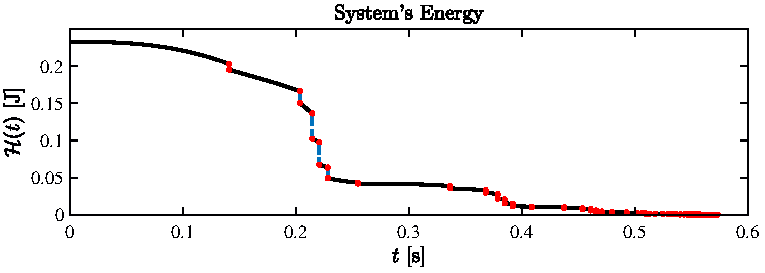
\includegraphics[width=\linewidth]{Figures/aut3.pdf}
	\caption[Uncontrolled system: time evolution of the Hamiltonian function.]{Uncontrolled system: time evolution of the Hamiltonian function. Due to system's passivity, the energy monotonically decreases to zero both during flow and jumps.}
	\label{fig:aut3}
\end{figure}
%
\begin{figure}[h]
	\centering
	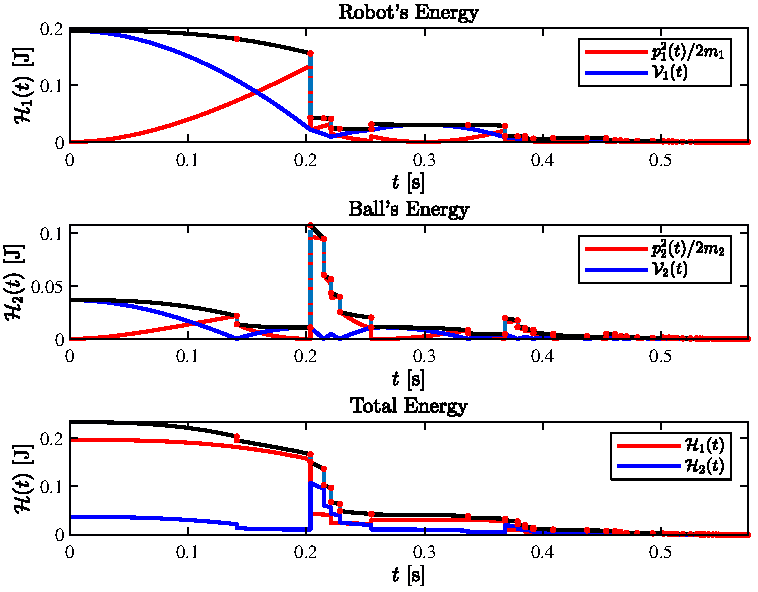
\includegraphics[width=\linewidth]{Figures/aut4.pdf}
	\caption[Uncontrolled system: Energy distribution within the system.]{Uncontrolled system: Energy distribution within the system. Trajectories happen on decreasing level--sets of $\Ha$, even if $\Ha_1$ and $\Ha_2$ may locally increase after some ball--robot impacts.}
	\label{fig:aut4}
\end{figure}
%
%
It can be noticed that $\Ha$ presents a monotonically decreasing trend, in both flows (due to the viscous friction terms) and jumps (since the restitution coefficients are less than one). In fact, trajectories happen on decreasing level--sets of $\Ha$, even if $\Ha_1$ and $\Ha_2$ may locally increase after some ball--robot impacts. Moreover, from the figures it is easily to verify the asymptotic stability and attractivity of the origin ($x = \mymathbb{0}_4$) and the \textit{Zeno behavior} of the autonomous system (see \cite{goebel2009hybrid}).
%%%%%%%%%%%%%%%%%%%%%%%%%%%%%%
\subsection{Controlled System}
%
Simulations of the system controlled via iterative energy shaping have also been performed. The control parameters have been chosen as: $k_{p,w} = 10^4$, $k_{d,w} = 10^3$, $\delta = 0.05$m, $k_0 = 10$, $k_{d,h} = 0$, $\varphi_\xi(e) = 10e + 100\sum_{i = 1}^{\xi}e(i)$, $q_{2,max}^* = 0.1$m. The time evolution of the state variables are shown in Figs. \ref{fig:ctrl1} and \ref{fig:ctrl1_det}.
%
\begin{figure}[!h]
	\centering
	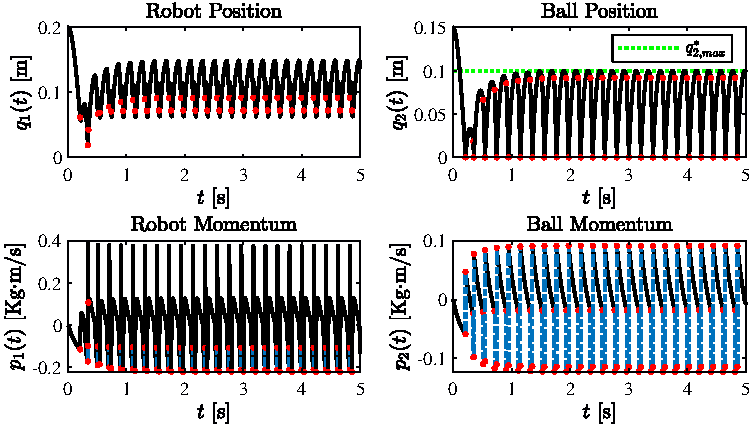
\includegraphics[width=\linewidth]{Figures/ctrl1.pdf}
	\caption[Iterative energy shaping control: time evolution of the robot and ball states]{Iterative energy shaping control: time evolution of the robot and ball states (position and momentum). Red dots correspond to system's jumps while dashed blue lines highlight discontinuous state changes. Notice that the ball states converge on a periodic trajectory reaching at each bounce the desired peak $q^*_{2,max}$ (dotted green line).}
	\label{fig:ctrl1}
\end{figure}
%
%
\begin{figure}[!h]
	\centering
	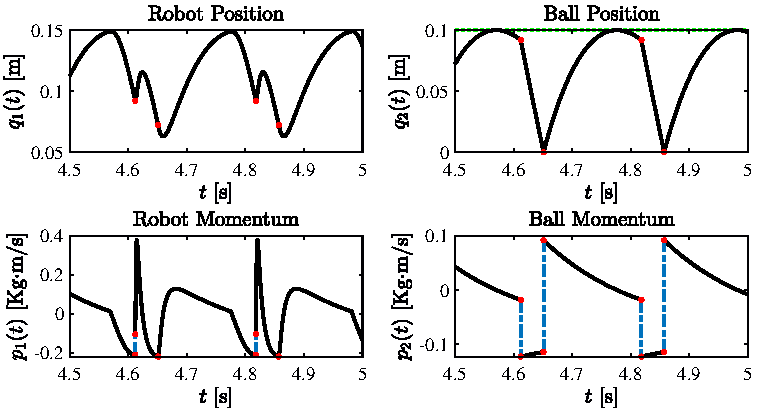
\includegraphics[width=\linewidth]{Figures/ctrl1_det.pdf}
	\caption[Iterative energy shaping control: detailed view of the time evolution of the ball and robot positions at steady state]{Iterative energy shaping control: detailed view of the time evolution of the ball and robot positions at steady state.}
	\label{fig:ctrl1_det}
\end{figure}
%
%
Notice that the trajectory of the ball becomes periodic (asymptotically), reaching at each bounce the desired peak $q_{2,max}^*$, proving the effectiveness of the proposed control scheme. Furthermore, the time evolution of the energy function is shown in Figs. \ref{fig:ctrl3} and \ref{fig:ctrl3_det} while Figs. \ref{fig:ctrl4} and \ref{fig:ctrl4_det} show how the energy flows across the system during each period. 
%
\begin{figure}[!h]
	\centering
	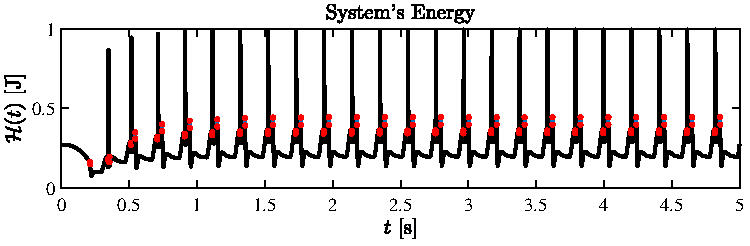
\includegraphics[width=\linewidth]{Figures/ctrl3.pdf}
	\caption{Iterative energy shaping control: the time evolution of the Hamiltonian function. After a short transient also the system's energy becomes periodic.}
	\label{fig:ctrl3}
\end{figure}
%
\begin{figure}[!h]
	\centering
	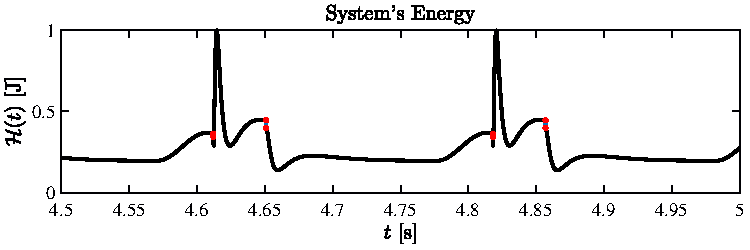
\includegraphics[width=\linewidth]{Figures/ctrl3_det.pdf}
	\caption{Iterative energy shaping control: detailed view of the time evolution of the Hamiltonian function at steady state to highlight its (asymptotic) periodicity.}
	\label{fig:ctrl3_det}
\end{figure}
%
\begin{figure}[!h]
	\centering
	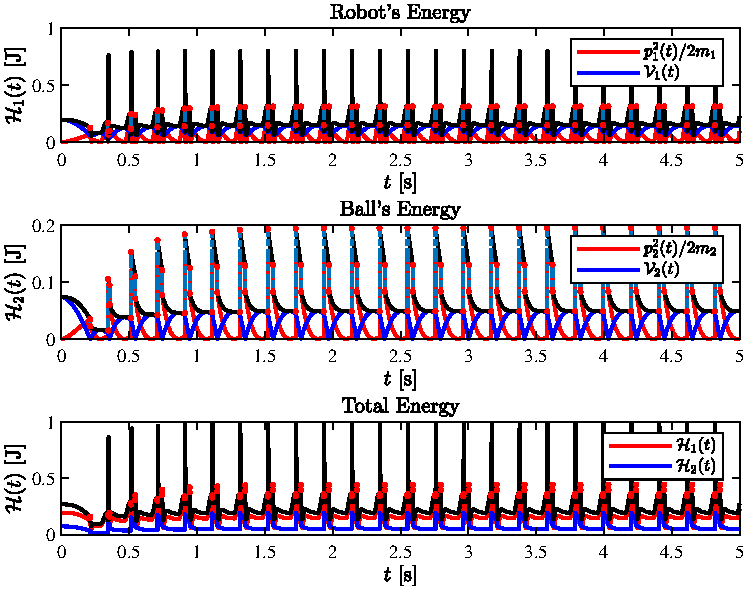
\includegraphics[width=\linewidth]{Figures/ctrl4.pdf}
	\caption{Iterative energy shaping control: the time evolution of the Hamiltonian function. After a short transient also the system's energy becomes periodic.}
	\label{fig:ctrl4}
\end{figure}
%
\begin{figure}[!h]
	\centering
	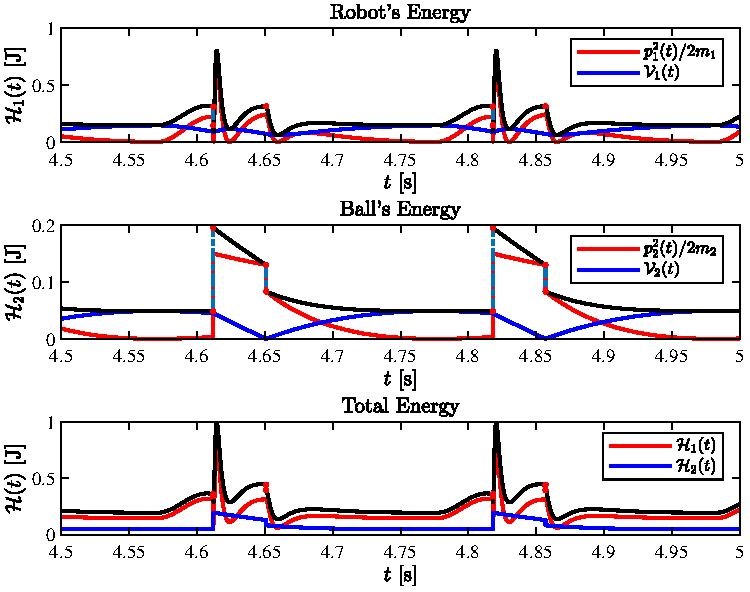
\includegraphics[width=\linewidth]{Figures/ctrl4_det.pdf}
	\caption{Iterative energy shaping control: detailed view of the time evolution of the Hamiltonian function at steady state to highlight its (asymptotic) periodicity.}
	\label{fig:ctrl4_det}
\end{figure}
%
As expected also the energy becomes periodic. In fact, the energy at the beginning and at the end of each cycle (bounce) become exactly the same. Moreover, we can see that, at steady state, during the ball--robot impact, the robot transfers to the ball the exact amount of energy necessary to reach the desired bounce peak. Finally, as shown in Fig. \ref{fig:ctrl5} the error goes to zero with the number of cycles.
%
\begin{figure}[!h]
	\centering
	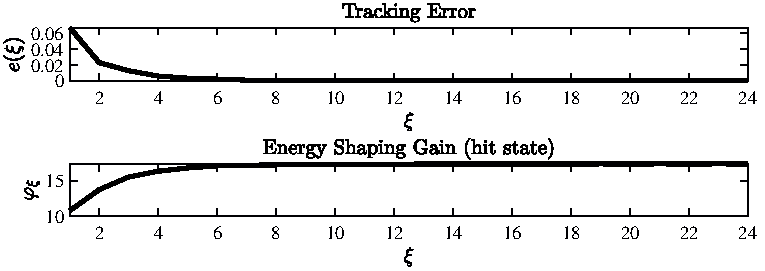
\includegraphics[width=\linewidth]{Figures/ctrl5.pdf}
	\caption{Iterative energy shaping control: (discrete) time evolution of the tracking error $e$ and of the energy shaping gain $\varphi_\xi(e)$. As the number of cycles $\xi$ increases, the tracking error $e$, i.e. the difference between the desired and ball's bounce peak, goes asymptotically to zero. Instead, the energy shaping gain converges, increasing monotonically, to a constant value.}
	\label{fig:ctrl5}
\end{figure}
%
On the other hand, the function $\varphi_\xi(e)$ converges exponentially to a positive constant value. 
%
A final consideration about the convergence of the system to the desired periodic trajectory can be made from the phase-space portrait of the system's trajectory (Fig. \ref{fig:ctrl2}). Being the time represented by the color transition, it can be noticed that the system approaches a limit cycle, an attractive asymptotically periodic trajectory, in which the tracking error is zero.
%
%
\begin{figure}[!h]
	\centering
	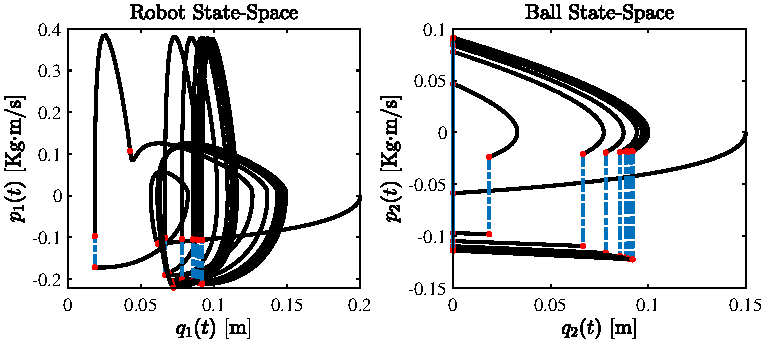
\includegraphics[width=\linewidth]{Figures/ctrl2.pdf}
	\caption[Iterative energy shaping control: phase--space trajectories]{Iterative energy shaping control: projections on the $q_1-p_1$ plane (above) and the $q_2-p_2$ plane (below) of the phase-space trajectory of the system. The system converges to a hybrid limit cycle in which $e=0$.}
	\label{fig:ctrl2}
\end{figure}
%
\clearpage
%
\subsection{Numerical Stability and Robustnes Analysis}
%
\subsubsection{Robustness to Initial Condition}
In order to prove the numerically the stability and robustness of the proposed control scheme, a Monte Carlo experiment similar to the one proposed in Section \ref{sec:analysis_aut}, has been performed. In particular, choosing as physical parameters $m_1=0.1\text{Kg}$, $m_2=0.15\text{Kg}$, $\beta_1=0.2$, $\beta_2=0.3$, $c_1=c_2=0.8$ and control parameters $k_{p,w} = 10^4$, $k_{d,w} = 10^3$, $\delta = 0.5$, $\sigma = 10$, $k_{d,h} = 10^2$, $\varphi_\xi(e) = 3000 + 10e + 300\sum_{i = 1}^{\xi}e(i)$, $q_{2,max}^* = 1$, 3000 trajectories has been computed starting from initial conditions $\xb_0^i$ sampled by the normal distribution
%
\begin{equation}
    \N(\xb_0,\sigma\mathbb{I}_n)
\end{equation}
%
with $\xb_0\triangleq(2,1.5,0,0)$ and $\sigma=1$. The time evolution of the system's state in all the trials is shown in Fig. \ref{fig:reg1}.
%
\begin{figure}[h]
    \centering
    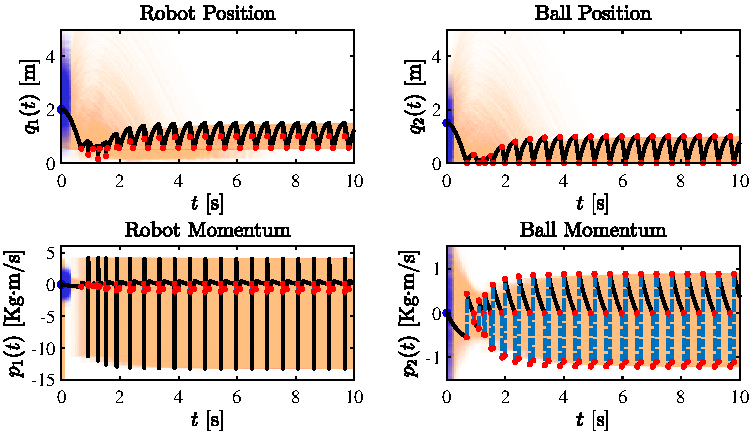
\includegraphics[width = \linewidth]{Figures/reg1.pdf}
    \caption[Time evolution of the controlled system' state in the Monte Carlo simulation]{Time evolution of the controlled system' state in the Monte Carlo simulation. The black trajectory is the nominal one (starting from $\xb_0$), where red dots and dashed blue lines indicate discrete events (impacts) and the value of the state after the events, respectively. Orange lines show the traces of all the other trajectories of the Monte Carlo runs (with initial condition sampled from $\N(\xb_0,\sigma\mathbb{I}_n)$). The blue dots at $t=0$ are the initial conditions. It can be noticed how trajectories, starting far from each other, eventually converge to the nominal trajectory.}
    \label{fig:reg1}
\end{figure}
%
The black trajectory is the nominal one (starting from $\xb_0$), where red dots and dashed blue lines indicate discrete events (impacts) and the value of the state after the events, respectively. Orange lines show the traces of all the other trajectories of the Monte Carlo runs (with initial condition sampled from $\N(\xb_0,\sigma\mathbb{I}_n)$). The blue dots at $t=0$ are the initial conditions. It can be noticed how trajectories, starting far from each other, eventually converge to the nominal trajectory. This means that the controller generates an attractive limit cycle. This can be seen indeed also in Fig. \ref{fig:reg2} where the phase--space trajectories are represented.
%
\begin{figure}[h]
    \centering
    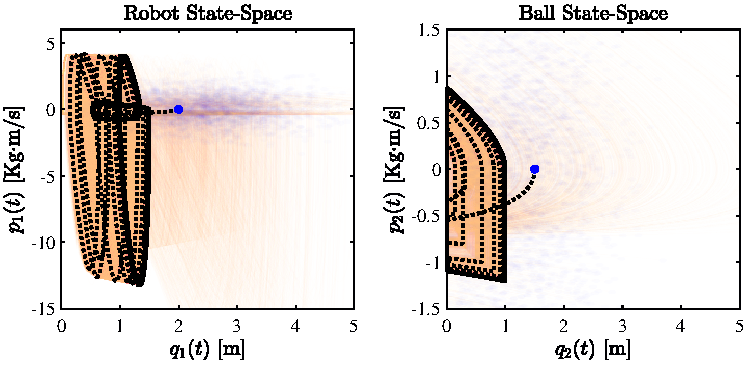
\includegraphics[width = \linewidth]{Figures/reg2.pdf}
    \caption[Phase--space trajectory of the controlled system in the Monte Carlo simulation]{Phase--space trajectory of the controlled system in the Monte Carlo simulation. The dashed black line is the nominal one (starting from $\xb_0$). Orange lines show the traces of all the other trajectories of the Monte Carlo runs (with initial condition sampled from $\N(\xb_0,\sigma\mathbb{I}_n)$). The blue dots at are the initial conditions. It can be noticed how trajectories, starting far from each other, eventually converge to the nominal trajectory.}
    \label{fig:reg2}
\end{figure}
%
\begin{figure}[!h]
    \centering
    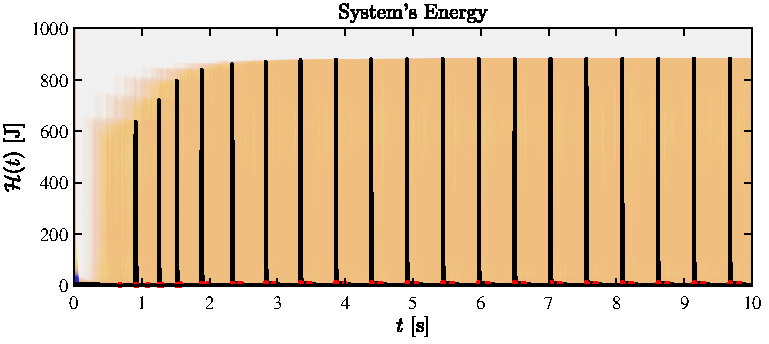
\includegraphics[width = \linewidth]{Figures/reg3.pdf}
    \caption[Time evolution of the energy in the Monte Carlo simulation]{Time evolution of the energy in the Monte Carlo simulation. The black trajectory is the nominal one (starting from $\xb_0$), where red dots indicate discrete events (impacts). Orange lines show the traces of all the other trajectories of the Monte Carlo runs (with initial condition sampled from $\N(\xb_0,\sigma\mathbb{I}_n)$). The blue dots at $t=0$ are the initial energies of each Monte Carlo run.}
    \label{fig:reg3}
\end{figure}

The time evolution of the energy (Hamiltonian function) among the Monte Carlo runs is also shown in Fig. \ref{fig:reg3}.
%
\subsubsection{Robustness to Change of Reference}
%
\clearpage
%%%%%%%%%%%%%%%%%%%%%%%%%%%%%%%%%%%%%%%%%%%%%%%%%%%%%%%%%%%%%%%%
\section{Summary}\label{sec:concl}
%
In this chapter, inspired by the theory developed in Chapter \ref{chap:HPH_systems}, a new paradigm of energy based control for the ball--dribbling robot, the \textit{iterative energy shaping}, has been introduced. Numerical simulations have been performed to prove the effectiveness of the proposed control scheme. Future work will include an additional formalization of the framework of \textit{hybrid port--Hamiltonian} systems, e.g. well--posedness, Lyapunov theory etc., and the exploration of the stabilization properties of the {iterative energy shaping} controllers for general hybrid systems.
%\definecolor{brickred}{rgb}{0.8, 0.25, 0.33}
%
\chapter{Multistable Energy Shaping of Linear--Time--Invariant Systems with Hybrid Mode Selector}

\label{chap:multistable}
\minitoc

\thispagestyle{empty}

\newpage
%%%%%%%%%%%%%%%%%%%%%%%%%%%%%%%%%%%%%%%%%%%%%%%%%%%%%%%%%%%%%%%%%%%%%%%%%%%%%%%
\section{Introduction}
\lettrine[lines=4]{\color{brickred}E}{xponentially} stable linear--time--invariant (LTI) systems admit a unique equilibrium point, while in many practical situations, they have to operate in a finite number of \textit{working modes} (fixed values of voltages, positions, etc.).
Thus, with standard linear control techniques, a continuous exogenous reference signal must be constantly provided in order to achieve the desired behaviour, e.g. asymptotic stabilisation of a desired set points. The block diagram of classical PID Control scheme is reported in Fig. \ref{fig:PID}.
%
\begin{figure}[!h]
	\centering
	    %\input{blockdiag.tex}
    \tikzstyle{block} = [draw, fill=gray!20, rectangle, 
    minimum height= 1em, minimum width= 1em]
\tikzstyle{sum} = [draw, fill=gray!50, circle, node distance=0.7cm]
\tikzstyle{input} = [coordinate]
\tikzstyle{output} = [coordinate]
\tikzstyle{pinstyle} = [pin edge={to-,thin,black}]
\tikzset{container/.style={draw, rectangle, dashed, inner sep=0.3em }}

% The block diagram code is probably more verbose than necessary
\begin{tikzpicture}[auto, node distance=1.4cm,>=latex']
    % We start by placing the blocks
    \node [input, name=input] {};
    \node [sum, right of=input] (sum) {};
    \node [block, right of=sum] (PID) {PID};
    \node [block, right of=PID] (B) {$\Bb$};
    \node [sum, right of=B] (sum2) {};
    \node [block, right of=sum2] (int) {$\int$};
    \node [block,below of = int,node distance =1.75em](A){$\Ab$};
    \node [block, right of=int, node distance=1.5cm] (system) {$\mathbf{C}$};
    %
    \node [output, right of=system] (output) {};
    \node [output, right of=output, node distance = 0.5 cm] (output2) {};
    % 
    \draw [draw,->] (input) -- node {$\mathbf{r}(t)$} (sum);
    \draw [->] (sum) -- node {$\mathbf{e}(t)$} (PID);
    \draw [->] (PID)-- node {$\mathbf{u}(t)$} (B);
    \draw [->] (B)--(sum2);
    \draw [->] (sum2) -- node {$\dot{\xb}$} (int);
    \draw [-latex] (int) -- node[name=u] {$\xb$} (system); 
    \draw [-] (system) -- node [name=y] {$\yb$}(output);
    \draw [->] (output) -- (output2); 
    % 
    \draw [->] (u) |- (A);
    \draw [->] (A) -| (sum2);
    %\connect{output}{sum};
    \draw[->] (output) |- node[below right,pos=0.2]{} ++(-1,-1.2) -| (sum);     
\end{tikzpicture}
	%
	\caption{A block representation of the controlled system.}
	\label{fig:PID}
\end{figure}
%
In order to embed in the controlled system the information on the desired working modes, a nonlinear controller is employed to simultaneously stabilise multiple points, i.e. achieve \textit{multistability} and avoid the need of external reference signals.
The introduction of the nonlinear terms gives rise to interesting properties of the controlled system, e.g. the possibility of shaping the basins of attraction of the different fixed points.
Appealing studies on the inverse problem, i.e., turning \textit{monostable} a {multistable} nonlinear system, have already been presented by \cite{PISARCHIK2014167}.

In this chapter, considering that stable LTI system can be made passive through an opportune choice of input and output (\cite{byrnes91}), a nonlinear controller able to stabilize multiple points is designed following a port-Hamiltonian paradigm, (\cite{876703,secchi2007control,ortega2008control,van2014port}). Then, in order to switch among the working modes, a \textit{mode selector} is developed exploiting the theory of hybrid dynamical systems (\cite{van2000introduction,goebel2008}).

Moreover, it is shown that the controlled system falls in the framework of hybrid port--Hamiltonian systems, proving the generality and applicability of the newly developed theory.
%

\clearpage

%%%%%%%%%%%%%%%%%%%%%%%%%%%%%%%%%%%%%%%%%%%%%%%%%%%%%%%%%%%%%%%%%%%%%%%%%%%%%%%%%%%%%%%%%%%%
\section{Multistable Energy Shaping of LTI Systems}\label{sec:multistable}
%
%%%%%%%%%%%%%%%%%%%%%%%%%%%%%%%%%%%%%%%%
In this section a nonlinear feedback law for a LTI system is designed to stabilise multiple fixed points. Passivity and the properties of passive LTI systems are briefly discussed.
%%%%%%%%%%%%%%%%%%%%%%%%%%%%%%%%%%%%
\subsection{Passivity of LTI Systems}
%
Let us consider the stable LTI specialization of (\ref{eq:nlaffine}), i.e. the standard system with state space realization
%
\begin{equation}\label{eq:lsys}
\left\{
\begin{matrix*}[l]
\dot{\xb}(t) = \Ab\xb(t) + \Bb\ub(t)\\
\yb(t) = \Cb\xb(t)
\end{matrix*}
\right.
\end{equation}
with system matrices $(\Ab\preceq 0,\Bb,\Cb)$ of appropriate dimensions.
%
{
It is easy to verify that, once system (\ref{eq:lsys}) is equipped with a quadratic storage function 
\begin{equation}
    \Ha(\xb) = \frac{1}{2}\xb^\top \Pb\xb,~\Pb = \Pb^\top \succ 0,
\end{equation}
it enjoys the KPY property, i.e. it is passive, if and only if
%
\begin{equation}\label{eq:KYPLTI}
        \Ab^\top \Pb + \Pb\Ab \leq 0\quad
        \Bb^\top \Pb = \Cb.
    %\end{matrix*}
    %\right.
\end{equation}
%
\begin{rem}
    It is worth to be noticed that passivity could just be tested by the definition:
    $(\Ab,\Bb,\Cb)$ is passive if and only if it is dissipative with respect to the supply rate $\langle \yb,\ub \rangle\triangleq \yb^\top \ub$, i.e.,  if and only if there exists $\Ha\in\C^1$,
    %
    \begin{equation}
        \dot{\Ha}\leq \yb^\top \ub
    \end{equation}
    %
    Thus, it yields,
    %
    \begin{align*}
        \dot{\Ha} =  \frac{1}{2}\xb^\top \left(\Ab^\top \Pb + \Pb\Ab\right)\xb + \xb^\top \Pb\Bb\ub \leq \xb^\top \Cb^\top \ub
    \end{align*}
    %
    which is true if and only if (\ref{eq:KYPLTI}) hold.
\end{rem}
%
Furthermore, for system (\ref{eq:lsys}) with ($\Ab\succeq0$) and $\ub=0$, the storage function is non increasing along trajectories, i.e.
%
\begin{equation*}
    \dot{\Ha}(\xb) =  \xb^\top \Pb\Ab\xb \leq 0\quad\forall \xb\in\X.
\end{equation*}
%
This means that the \textit{natural} dissipation inferred by the choice of $\Pb$ of the autonomous system corresponds to $\xb^\top \Pb\Ab\xb$ where $\Pb\Ab\preceq0$. 

}
%
In order to present clearly the upcoming concepts, the following prototype linear system has been chosen as example to be invoked throughout the chapter.
%
\begin{exmp}\label{ex:msd_MES}
    Consider a forced mass--spring--damper system of example \ref{ex:msd} with unitary mass, i.e. $m = 1$, $p = \dot{q}$ and $\xb\triangleq (q,p)$.
    The LTI state--space (\ref{eq:lsys}) representation is
    %
    \begin{equation}
        \dot{\xb} = \underbrace{\begin{bmatrix}0&1\\-k&-b\end{bmatrix}}_{\Ab}\xb+ \underbrace{\begin{bmatrix}0\\1\end{bmatrix}}_{\Bb}u.
    \end{equation}
    %
    The autonomous system is exponentially stable if $b>0$. Let $\Pb=\diag({k,1})$ be 
    Indeed $\Pb=\Pb^\top\succ0$ and $\Pb\Ab\prec0$. Thus, the system is passified (with storage function $\Ha = \frac{1}{2}\xb^\top \Pb\xb$) choosing the linear output as $\yb \triangleq \Bb^\top \Pb\xb = \dot{q}$, as also derived by first principles in Chapter \ref{chap:preliminaries}. Note that $\Ha$ is the total energy of the system. In general, any mechanical systems is passive with its total energy as storage function by choosing as input(s) the (generalised) forces and as output(s) the (generalised) momenta.
\end{exmp}
%
%Now let us briefly review port--Hamiltonian systems and their properties, since they represent the framework where PBC has been consistently developed (\cite{ortega2001putting}).

%%%%%%%%%%%%%%%%%%%%%%%%%%%%%%%%%%%%%%%%%%%%%%
% \subsection{Port--Hamiltonian Systems and PBC}
% %
% A port--Hamiltonian (PH) system (\cite{van2014port}) has an input--state--output representation\footnote{From now on, the dependency on $x$ of the scalar function $\Ha$ is hidden for compactness.}:
% \begin{equation}\label{eq:PH}
%     \left\{
%     \begin{matrix*}[l]
%     \dot{x} = \left[\Jb(x)-\Rb(x)\right](\partial\Ha)^\top + \mathcal{G}(x)u\\
%     y = \mathcal{G}^\top(x)(\partial \Ha)^\top
%     \end{matrix*}
%     \right.
% \end{equation}
% %
% which is in the form (\ref{eq:nlaffine}) where $\Jb(x)$ is a skew symmetric matrix representing the power preserving interconnections, $\Rb(x)$ is a symmetric positive semidefinite matrix representing the dissipation of the system and $\mathcal{G}(x)$ is a matrix representing the way in which external power is distributed into the system.
% %%%%%%%%%%%%%%%%%%%%%%
% {
% Furthermore, $\X$ is an $n$--dimensional manifold, $\mathcal{U}$ is a $m$--dimensional vector space and %and the input is a power conjugated variable (see \cite{van2014port});The output vector space 
% $\mathcal{Y} = \mathcal{U}^*$ is its dual space;
% %defined as the dual space of $\mathcal{U}$ so that 
% $y^\top u$ has the unit measure of power (\cite{secchi2007control}). 

% %
% }
% %%%%%%%%%%%%%%%%%%%%%%
% The power conservation property of (\ref{eq:PH}) is defined by the power--balance equation
% \[\frac{d\Ha}{dt} = \partial\Ha\dot{x}= -\partial\Ha\Rb(\partial\Ha)^\top + y^\top u\leq y^\top u\]
% i.e., PH systems are passive.
% %
% \begin{prob}[Passivity--based control]
% Consider a PH system (\ref{eq:PH}). A control action $u = \beta(x) + v$ solves the PBC problem if the closed-loop system satisfies a desired power-balance equation
% %
% \begin{equation*}
% 	%\frac{d\Ha^*}{dt} 
% 	\dot{\Ha}^*
% 	= z^\top v - d^*
% \end{equation*}
% where $\Ha^*$ is the desired energy function, $d^*$ the desired dissipation function and $z\in\R^m$ the new power conjugated (passive) output.
% \end{prob}
% %\begin{center}\fbox{\begin{minipage}{23em}
% %
% %\end{minipage}}\end{center}
% %f
% The most common solution to the PBC problem is the \textit{energy--balancing PBC} (EB--PBC) proposed by \cite{876703}. Roughly speaking, the controller is obtained directly from the power balance equation by setting the desired dissipation $d^*$ equal to the natural dissipation of the system, i.e, $d^* \triangleq \partial\Ha\Rb(\partial\Ha)^\top$ and keeping the same output $z \triangleq y$. Next proposition gives an operative insight of how to accomplish the EB--PBC control task
% \begin{prop}[\cite{secchi2007control}]
% If it is possible to find a function $\beta(x)$ such that
% \begin{equation*}
%     %\frac{d\Ha_a}{dt} 
%     \dot{\Ha}_a
%     =y^\top\beta(x)
% \end{equation*}
% then the control law $u = \beta(x)+v$ is such that 
% \begin{equation*}
%     %\frac{d\Ha^*}{dt} 
%     \dot{\Ha}^*
%     = y^\top v -d^*
% \end{equation*}
% is satisfied for $\Ha^* \triangleq \Ha+\Ha_a$.
% \end{prop}
% This implies that the state feedback $\beta(x)$ is such that the \textit{added energy} $\Ha_a$ equals the energy supplied to the system and, consequently, $\Ha^*$ is the difference between the stored and supplied energy.
% In  \cite{ortega2008control} the closed-form solution of the EB--PBC controller is given by 
% \[\beta(x) = -\mathcal{G}^+\left[\Jb-\Rb\right]^\top(\partial\Ha_a)^\top\]
% where $\mathcal{G}^+$ is the left pseudoinverse of $\mathcal{G}$ and $\Ha_a$ satisfies the following matching equations 
% \[\begin{bmatrix}\mathcal{G}^{\perp}\left[\Jb-\Rb\right]^\top\\\mathcal{G}^\top\end{bmatrix}(\partial\Ha_a)^\top = \mathbb{0}_{n+m}\]
% being $\mathcal{G}^{\perp}$ a left full--rank annihilator of $\mathcal{G}$.

% The idea behind this state--feedback control is to ``shape'' the energy function so that its only minimum translates towards a new minimum, representing the desired working condition of the controlled system (e.g. \textit{PD + gravity compensation} in robot regulation, {\cite{secchi2007control}). In the following it is shown how this concept can be extended to produce multiple stable working conditions by means of a nonlinear feedback law applied to an LTI system (\ref{eq:lsys}).
%
\subsection{Multistable Passivity--Based Control of LTI Systems}
%
Any passive LTI system (\ref{eq:lsys}) with storage function $\Ha(\xb) = \frac{1}{2}\xb^\top \Pb\xb$ such that $\Null(\Pb)$ $\subseteq$ $\Null(\Ab)$ admits a port-Hamiltonian representation\footnote{Since we choose $\Pb>0$, this condition does not represent a loss of generality, i.e. any system (\ref{eq:lsys}) can be written in PH form.}:
%
\begin{equation}
    \left\{
    \begin{matrix*}[l]
    \dot{\xb} = \left[\Jb-\Rb\right]\Pb\xb + \Bb\ub\\
    \yb = \Bb^\top \Pb\xb
    \end{matrix*}
    \right.
\end{equation}
%
where 
%
\begin{equation}
    \Jb \triangleq \frac{1}{2}(\Ab\Pb^{-1}-\Pb^{-1}\Ab^\top),\quad\Rb \triangleq- \frac{1}{2}(\Ab\Pb^{-1}+\Pb^{-1}\Ab^\top).
\end{equation}
% 
are derived by the following relations:
%
\begin{align}
    & \Ab = \left[\Jb-\Rb\right]\Pb\\
    & \left(\Jb-\Rb\right)^\top + \left(\Jb-\Rb\right) = -2\Rb.
\end{align}
%
Thus, for a LTI system, the energy balancing control law (\ref{eq:ebpbc}) becomes 
%
\begin{align}\label{eq:multiebpbc_lin}
    \bm\beta(\xb) &= -\left(\Bb^\top\Bb\right)^{-1}\Bb^\top\Pb^{-1}\Ab^\top\bm\nabla\Ha_a
\end{align}
%
with
%
\begin{equation}
    \Ha_a\triangleq\Ha^*-\frac{1}{2}\xb^\top \Pb\xb
\end{equation}
%
and the matching conditions:
%
\begin{equation}\label{eq:match_lin}
    \begin{bmatrix}
        {\Bb}^{\perp}\left[\Jb-\Rb\right]^\top\\
        {\Bb}^\top
    \end{bmatrix}
    %
    \bm\nabla\Ha_a =\mymathbb{0}_{n+m}.
\end{equation}
%
\begin{prop}[Multistable EB--PBC of LTI System]
	Consider a passive LTI system (\ref{eq:lsys}) equipped with a quadratic storage function $\Ha(\xb) = \frac{1}{2}\xb^\top \Pb\xb$. Let $\Ha^*\in\C^2$ be a desired storage (energy) function with $p$ minima corresponding to $p$ desired equilibrium points $\xb^*_i$, i.e.
	%
	\begin{equation}
	\bm\nabla\Ha^*\big|_{\xb = \xb^*_i} = \mymathbb{0}_n,~~~ \bm\nabla^2 \Ha^*\big|_{\xb = \xb^*_i}>0\quad\forall i = 1,\dots,p.
	\end{equation}
	%
	The EB--PBC control action (\ref{eq:multiebpbc_lin})
	%
	stabilises the desired equilibrium points $\xb^*_i$ if (\ref{eq:match_lin}) holds true for the chosen $\Ha^*$.
    %
\end{prop}
%
\proof
The proof follows similarly to \citep{ortega2008control}. Indeed, the minimum points of $\Ha^*$ will result to be Lyapunov stable equilibria in the same way in which EB--PBC acts on a single fixed point. It follows that if $\Ab$ is Hurwitz, the new ``shaped'' energy $\Ha^*$ will be monotonically decreasing along any trajectory since $\Ab^\top \Pb + \Pb\Ab\prec 0$ and, thus, if it is bounded from below the system will reach asymptotically one of the minima of $\Ha^*$. However, if the linear system is only stable, i.e. $\Ab^\top \Pb + \Pb\Ab\preceq 0$, then locally invariant sets have to be examined by means of La Salle’s invariance theorem to check asymptotic stability \citep{khalil2002nonlinear}.
\endproof
%
\begin{rem}
	Deeper evaluations and considerations on Lyapunov functions for multistable nonlinear systems are reported in \cite{efimov2012global}. It has to be underlined that, in order to have an energy function with multiple minima, it is necessary to have the presence of local maxima, which however do not affect global behaviour of the system, since those are just unstable fixed points of the closed loop system.
	
\end{rem}
%
Furthermore, in the case of LTI systems, the damping injection takes the form
\begin{equation}
    \vb = \mathbf{K}_d\Bb^\top\Pb\xb
\end{equation}
A block diagram  picturing the overall control scheme is represented in Fig. \ref{fig:block}.
%
\begin{figure}[!h]
	\centering
	    %\input{blockdiag.tex}
    \tikzstyle{block} = [draw, fill=gray!20, rectangle, 
    minimum height= 1em, minimum width= 1em]
\tikzstyle{sum} = [draw, fill=gray!50, circle, node distance=0.7cm]
\tikzstyle{input} = [coordinate]
\tikzstyle{output} = [coordinate]
\tikzstyle{pinstyle} = [pin edge={to-,thin,black}]
\tikzset{container/.style={draw, rectangle, dashed, inner sep=0.3em }}

% The block diagram code is probably more verbose than necessary
\begin{tikzpicture}[auto, node distance=1cm,>=latex']
    % We start by placing the blocks
    \node [input, name=input] {};
    \node [sum, right of=input] (sum) {};
    \node [block, left of=sum] (B) {$B$};
    \node [sum, left of=B] (sum2) {};
    \node [input, left of = sum2,name=input2] {};
    \node [block, right of=sum] (int) {$\int\cdot dt$};
    \node [block,below of = int,node distance =1.75em](A){$A$};
    \node [block,below of = A,node distance =1.8em](beta){$\beta(\cdot)$};%{$-B^+P^{-1}A^T(\partial\Ha_a)^T$};
    \node [block, right of=int, node distance=1.5cm] (system) {$B^\top P$};
    % We draw an edge between the controller and system block to 
    % calculate the coordinate u. We need it to place the measurement block. 
    \draw [-latex] (int) -- node[name=u] {$x$} (system);
    \node [output, right of=system] (output) {};
    \node [output, right of=output] (output2) {};
    \node [block, above of=u, node distance = 1.75em] (outfb) {$-\kappa$};
    %
    \node [container , fit = (beta), fill = blue!100, fill opacity=0.1] (nlctrl) {};
    \node at (nlctrl.east) [ right, node distance =2cm and -1cm, align = center] {\footnotesize{energy shaping control} $\newline$\\ {\footnotesize(nonlinear state feedback)}};
    %
    \node [container , fit = (outfb), fill = blue!100, fill opacity=0.1] (dampin) {};
    \node at (dampin.west) [left, node distance =2.5cm and 1cm, align = center] {\footnotesize{damping injection control} $\newline$\\ {\footnotesize{\color{white}aaaaaa}(output feedback)}};
    % Once the nodes are placed, connecting them is easy.
    % 
    \draw [draw,->] (input2) -- node {$\mathbb{0}_m$} (sum2);
    \draw [->] (sum) -- node {$\dot{x}$} (int);
    \draw [-] (system) -- node [name=y] {$y$}(output);
    \draw [->] (output) -- (output2);
    \draw [->] (output) |- (outfb);
    \draw [->] (outfb) -| node[pos=0.99] {} 
        node [near end] {$v$} (sum2);
    \draw [->] (u) |- (A);
    \draw [->] (A) -| (sum);
    \draw [->] (u) |- (beta);
    \draw [->] (beta) -| (sum2);
    \draw [->] (sum2)--(B);
    \draw [->] (B)--(sum);
\end{tikzpicture}
	%
	\caption{A block representation of the controlled system.}
	\label{fig:block}
\end{figure}
%
\subsection{Application Example \ref{ex:msd_MES}}
%
Consider the system in Example \ref{ex:msd_MES} and let the desired energy function have two symmetrically distributed minima on the displacement axes, e.g.,
%
\begin{equation}
    \Ha^*(q,p) = \lambda q^4-\mu q^2 + \frac{1}{2}p^2 + \frac{\mu^2}{4\lambda}\qquad\lambda,\mu>0
\end{equation}
%
which has two minima in $[\pm\sqrt{\mu/2\lambda},0]^\top$ and a local maximum in $[0,0]^\top$. The desired energy function is plotted in Figure \ref{fig:shaped_en}
%
\begin{figure}
    \centering
    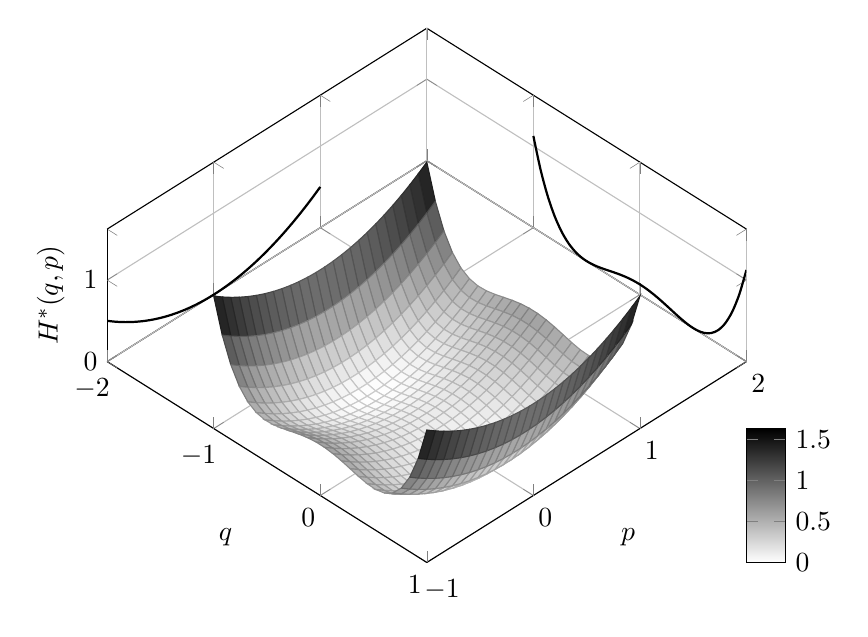
\begin{tikzpicture}[
  declare function = {lambda=2;},
  declare function = {mu=1;},
  declare function = {kin=(x^2)/2;},
  declare function = {pot(\l,\m)=\l*x^4 - \m*x^2 + (\m^2)/(4*\l);},
  declare function = {H(\l,\m)=\l*x^4 - \m*x^2  + (\m^2)/(4*\l)+ (y^2)/2;}]
  \begin{axis}[
    colormap  = {whiteblack}{color(0cm)  = (white);color(1cm) = (black)},
    width          = 0.8\linewidth,
    view           = {45}{65},
    enlargelimits  = false,
    grid           = major,
    domain         = -1:1,
    y domain       = -1:1,
    samples        = 26,
    xlabel         = $q$,
    ylabel         = $p$,
    zlabel         = {$\Ha^*(q,p)$},
    colorbar,
    colorbar style = {
      at     = {(1,0)},
      anchor = south west,
      height = 0.25*\pgfkeysvalueof{/pgfplots/parent axis height},
     % title  = {$P(x_1,x_2)$}
    }
  ]
    \addplot3 [surf] {H(lambda,mu)};
    \addplot3 [domain=-1:1,samples=31, samples y=0, thick, smooth]
     (x,2,{pot(lambda,mu)});
    \addplot3 [domain=-1:1,samples=31, samples y=0, thick, smooth]
      (-2,x,{kin});

    %\draw [black!50] (axis cs:-1,0,0) -- (axis cs:4,0,0);
    %\draw [black!50] (axis cs:0,-1,0) -- (axis cs:0,4,0);

    %\node at (axis cs:-1,1,0.18) [pin=165:$P(x_1)$] {};
    %\node at (axis cs:1.5,4,0.32) [pin=-15:$P(x_2)$] {};
  \end{axis}
\end{tikzpicture}
    \caption[Desired shaped energy function]{Desired shaped energy function $\Ha^*(q,p) = \lambda q^4-\mu q^2 + \frac{1}{2}p^2 + \frac{\mu^2}{4\lambda}$}
    \label{fig:shaped_en}
\end{figure}
%
Thus, 
%
\begin{align}
    \Ha_a & = \Ha^* - \Ha \\
          & = \lambda q^4-(\mu+\frac{1}{2}\kappa)q^2 + \frac{1}{2}p^2 + \frac{\mu^2}{4\lambda}
\end{align}
%
and, therefore
\[\bm\nabla\Ha_a = (4\lambda q^3-(2\mu + k)q,p).\]
It is easy to proof that the matching conditions (\ref{eq:match_lin}) of the EB--PBC are satisfied for $\Ha_a$. The energy shaping control law becomes
%
\begin{align}\label{eq:ex_ctrl}
    \beta(q) &= -\begin{bmatrix}0&1\end{bmatrix}\begin{bmatrix}0&-1\\1&-b\end{bmatrix}\begin{bmatrix}4\lambda q^3-(2\mu + k)q\\p\end{bmatrix}\nonumber\\
             &= -4\lambda q^3+(2\mu + k)q.
\end{align}
%
A numerical simulation of the proposed control scheme has been performed with $k = 1$, $b = 0.5$. The parameters $\lambda$ and $\mu$ have been set to $2$ and $1$ respectively, placing the minima of $\Ha^*$ in $[\pm0.5,0]^\top$. No damping injection actions has been added as the asymptotic stability is already guaranteed by the natural dissipation of the autonomous linear system. Starting in the initial position $\xb_0 \triangleq (-0.9,0)$ the system has been simulated for both the  autonomous and the multistable EB--PBC controlled system for $40s$. The resulting phase--space portraits are reported in Fig. \ref{fig:ctrl_ps}.
%
\begin{figure}[h]
    \centering
    \definecolor{ocean}{rgb}{0.00000,0.44700,0.74100}

\begin{tikzpicture}
\begin{axis}[
width=5cm,
height=5cm,
at={(1in,0.331in)},
view={0}{90},
%colorbar,
%point meta max=1,
%point meta min=0,
colorbar horizontal,
%colorbar style={
%	width=8cm,
	%xtick={0,0.5,...,30},
%	ylabel style={},
%	xticklabel pos=lower
%},
colormap = {whiteblack}{color(0cm)  = (white);color(1cm) = (black)},
colorbar style = {at = {(0,-0.25)}},
xmin=-1,
xmax=1,
xlabel style={font=\color{white!15!black},at = {(0.75in,-0.1in)}},
xlabel={$q(t)~[m]$},
ymin=-1,
ymax=1,
ylabel style={font=\color{white!15!black},at = {(-0.1in,0.75in)}},
ylabel={$p(t)~[ms^{-1}]$},
title = {uncontrolled},
axis background/.style={fill=white},
]
\addplot3[contour filled={number = 25,labels={false}},mesh/rows=50,mesh/cols=50,mesh/check=false,forget plot
] table {H.dat};
%
\addplot [color=ocean, line width=1.5pt]
table[row sep=crcr]{%
	-0.9	0\\
	-0.899985991795746	0.00501674269174762\\
	-0.899944019691303	0.0100193471557007\\
	-0.899874162931692	0.0150076971406221\\
	-0.89977650140532	0.0199816771641279\\
	-0.898873958295022	0.0446320420072224\\
	-0.897288646861763	0.0689062780415569\\
	-0.8950312582937	0.0927908195727069\\
	-0.892112845290034	0.116272595485913\\
	-0.868002952216995	0.227228035383425\\
	-0.829223766085857	0.326435243373571\\
	-0.777500187200184	0.412807338237014\\
	-0.714659008971771	0.485603292982159\\
	-0.600340602727355	0.570331414933827\\
	-0.471488130080395	0.621495133714803\\
	-0.335347897263502	0.640176352681101\\
	-0.198445114013884	0.628945422916099\\
	-0.0746437735806325	0.594456994280607\\
	0.0401381420897199	0.540383416283467\\
	0.142232199262124	0.470719359197013\\
	0.229035654600393	0.389586456149254\\
	0.290490142676407	0.313265041426897\\
	0.338339729122556	0.23421079930552\\
	0.372303052526759	0.154991891744638\\
	0.392571550535566	0.0778835525828194\\
	0.399731808807902	-0.00306277450207788\\
	0.391870981971099	-0.0763851640723532\\
	0.370660517667212	-0.14009523114136\\
	0.338087981923116	-0.192856605316552\\
	0.298136191440485	-0.232477962681855\\
	0.25184670416552	-0.260834031598041\\
	0.201350587767438	-0.277964416164619\\
	0.148664452554781	-0.284317405805023\\
	0.0907667653016975	-0.27983068280962\\
	0.0349146831770288	-0.264713991318473\\
	-0.0168257578844223	-0.240602883573134\\
	-0.0628664499768871	-0.20930778888674\\
	-0.0980374609679892	-0.17699717235111\\
	-0.127063690395628	-0.141926700215142\\
	-0.149546840710965	-0.105459101422993\\
	-0.165363769927057	-0.0688391130058303\\
	-0.17517242929207	-0.0298002370528735\\
	-0.177436179549933	0.00664995096132089\\
	-0.172778407588365	0.0393477927721653\\
	-0.162032775025325	0.0674497666527798\\
	-0.147454933577949	0.0889207675276733\\
	-0.129347064906398	0.10558047092737\\
	-0.108623814628922	0.117297644237556\\
	-0.086179982857339	0.124136300367046\\
	-0.0599942658276899	0.126273096752299\\
	-0.03394383333752	0.123024483749271\\
	-0.00911017489546286	0.115053707894857\\
	0.0136390018342169	0.103150490035125\\
	0.0323115311721372	0.0893174145892377\\
	0.0481096403624088	0.0735852869681779\\
	0.0607228554124504	0.0566997231192924\\
	0.0700087283561835	0.0393538111534125\\
	0.0761616883827873	0.0213703319404493\\
	0.0787495703594155	0.00429179247670834\\
	0.0780099609822195	-0.0112862674191978\\
	0.0742949609073913	-0.0249184536659205\\
	0.0676235361779361	-0.0368399446136417\\
	0.0587030242407405	-0.0459531423309749\\
	0.0481558122411435	-0.0521341873494105\\
	0.0365928902454288	-0.0554253293582465\\
	0.0240750228983752	-0.0559548535184\\
	0.0117514398745198	-0.0537959330321324\\
	0.00019941613886286	-0.0493329003279672\\
	-0.0101378207178845	-0.0430176266200058\\
	-0.019073150754024	-0.0351836299097121\\
	-0.0261146445062195	-0.0264793026690255\\
	-0.0311080878005064	-0.0174345850654783\\
	-0.0340432057031742	-0.00851368245135384\\
	-0.0350111008169466	0.000208271867982888\\
	-0.034025886560588	0.00794187081482636\\
	-0.0313546321013023	0.014373201383412\\
	-0.0273270827992865	0.0193247845816726\\
	-0.021776682313328	0.0229649845032737\\
	-0.0155344254822122	0.0247149856554559\\
	-0.00909170615632734	0.0246816915211178\\
	-0.00286371969873624	0.0230947709063524\\
	0.00280725028199055	0.0202496734322155\\
	0.00760795718689828	0.016477401614915\\
	0.0113249300742123	0.0121348606754593\\
	0.0138716616756584	0.00755763965809117\\
	0.0153115070918749	0.00268446415992479\\
	0.0154380718037925	-0.00174353700984352\\
	0.0144046855261442	-0.0054393994641403\\
	0.0124469315254243	-0.00824628912471304\\
	0.00973633834811147	-0.0101436953203082\\
	0.00663307131848225	-0.0109904365212177\\
	0.00344345203354436	-0.010849788231025\\
	0.000418598885933671	-0.00987679726686231\\
	-0.00236889674029977	-0.00817147420768934\\
	-0.00455610701932897	-0.00600636910422985\\
	-0.0060212570956228	-0.00363960519553869\\
	-0.00675662344583174	-0.00129708301418448\\
	-0.00679915540873005	0.000997090639439771\\
	-0.00615806076904666	0.0028415988465903\\
	-0.00499448977320246	0.00409954744618751\\
	-0.00350966028254127	0.0047525483255705\\
	-0.00178742736195878	0.00483753431425414\\
	-0.000142544164199142	0.00436296059647222\\
	0.001233863384226	0.00346409628606365\\
	0.00224352413019931	0.0023187867470898\\
	0.00286423019005585	0.001064908755426\\
	0.00304301781878184	-0.000107287213496858\\
	0.00281783500493549	-0.0010575880234264\\
	0.0022937627777237	-0.00172125518888289\\
	0.00153324548129663	-0.00210115118921709\\
	0.000699028537681449	-0.00212944532957787\\
	-7.39090484163769e-05	-0.00185022451593175\\
	-0.000696860580362937	-0.0013673867011887\\
	-0.00115698870029392	-0.000733929244931739\\
	-0.00134549775988726	-0.000103223462323883\\
	-0.00126431291907824	0.000412349861050412\\
	-0.000993032124110712	0.000759026310963054\\
	-0.000596744297566764	0.000936587972301828\\
	-0.0001714552068425	0.000909680277066964\\
	0.000192405808728558	0.000708505171052146\\
	0.000443835290730197	0.000417655115078066\\
	0.000582041712668234	8.20914139281743e-05\\
	0.000563673850896241	-0.000200244790181628\\
	0.000407680747611572	-0.000363593139831435\\
	0.000193602312173417	-0.000405181279185971\\
	-2.30281468151146e-05	-0.000352938747129361\\
	-0.000186564607289939	-0.000224639431191565\\
	-0.000253723590669539	-6.14216529346211e-05\\
	-0.000236476036563678	7.85096220374468e-05\\
	-0.000162705457701936	0.000174617140937539\\
	-5.64067851445571e-05	0.000196804176492543\\
	4.62570015027289e-05	0.000136732345109551\\
	0.000106953605066236	4.5051528543188e-05\\
	0.00012515523979931	-5.30186446630676e-05\\
	8.69067523052607e-05	-0.000109998447934223\\
	-2.80092519366811e-06	-9.06136603478964e-05\\
	-7.20860461539662e-05	-2.64132971781262e-05\\
	-7.64796094496801e-05	2.09540211186838e-05\\
	-5.84460433855426e-05	5.1911771294405e-05\\
	-2.42154646050572e-05	5.68361010025379e-05\\
	8.96341400149207e-06	4.27250166876023e-05\\
}
[postaction={decorate, decoration={markings,
		mark=between positions 0.4 and 1 step 1 with {\arrow[black,line width=1.5pt]{latex};}
}}]
;
\addplot [color=black, line width=1.0pt, draw=none, mark=*, mark options={solid, fill=red}]
table[row sep=crcr]{%
	0	0\\
};
\end{axis}
%
%
%%%%%%%%%%%%%%%%%%%%%%%%%%%%%%%%%%%%%%%%%%%%%%%%%%%%%%%%%%%%%%%%%%%%%%%%%%%%%%%%%%%%
%%%%%%%%%%%%%%%%%%%%%%%%%%%%%%%%%%%%%%%%%%%%%%%%%%%%%%%%%%%%%%%%%%%%%%%%%%%%%%%%%%%%
%%%%%%%%%%%%%%%%%%%%%%%%%%%%%%%%%%%%%%%%%%%%%%%%%%%%%%%%%%%%%%%%%%%%%%%%%%%%%%%%%%%%
%%%%%%%%%%%%%%%%%%%%%%%%%%%%%%%%%%%%%%%%%%%%%%%%%%%%%%%%%%%%%%%%%%%%%%%%%%%%%%%%%%%%
%%%%%%%%%%%%%%%%%%%%%%%%%%%%%%%%%%%%%%%%%%%%%%%%%%%%%%%%%%%%%%%%%%%%%%%%%%%%%%%%%%%%
%%%%%%%%%%%%%%%%%%%%%%%%%%%%%%%%%%%%%%%%%%%%%%%%%%%%%%%%%%%%%%%%%%%%%%%%%%%%%%%%%%%%
%%%%%%%%%%%%%%%%%%%%%%%%%%%%%%%%%%%%%%%%%%%%%%%%%%%%%%%%%%%%%%%%%%%%%%%%%%%%%%%%%%%%
%%%%%%%%%%%%%%%%%%%%%%%%%%%%%%%%%%%%%%%%%%%%%%%%%%%%%%%%%%%%%%%%%%%%%%%%%%%%%%%%%%%%
%%%%%%%%%%%%%%%%%%%%%%%%%%%%%%%%%%%%%%%%%%%%%%%%%%%%%%%%%%%%%%%%%%%%%%%%%%%%%%%%%%%%
%%%%%%%%%%%%%%%%%%%%%%%%%%%%%%%%%%%%%%%%%%%%%%%%%%%%%%%%%%%%%%%%%%%%%%%%%%%%%%%%%%%%
%
%
\begin{axis}[
width=5cm,
height=5cm,
at={(2.7in,0.331in)},
view={0}{90},
%point meta max=1,
%point meta min=0,
colorbar horizontal,
colorbar style = {at = {(0,-0.25)}},
colormap = {whiteblack}{color(0cm)  = (white);color(1cm) = (black)},
xmin=-1,
xmax=1,
xlabel style={font=\color{white!15!black},at = {(.75in,-0.1in)}},
xlabel={$q(t)~[m]$},
ymin=-1,
ymax=1,
ylabel style={font=\color{white!15!black},at = {(-0.1in,0.75in)}},
ylabel={$p(t)~[ms^{-1}]$},
title = {controlled},
axis background/.style={fill=white},
]
\addplot3[contour filled={number = 25,labels={false}},mesh/rows=50,mesh/cols=50,mesh/check=false,forget plot
] table {Hs.dat};
%
\addplot [color=ocean, line width=1.5pt]
table[row sep=crcr]{%
	-0.9	0\\
	-0.899996870908082	0.00502218565295018\\
	-0.899987486315726	0.0100411075881561\\
	-0.899971850372859	0.0150566320023799\\
	-0.899949967395858	0.0200686252832798\\
	-0.899747009487171	0.0450709682895715\\
	-0.899388618721859	0.0699651105069001\\
	-0.89887552042962	0.0947346192697363\\
	-0.898208541398208	0.119363260804648\\
	-0.892600993178684	0.239855894760487\\
	-0.88332728745733	0.354537716060326\\
	-0.870592934007952	0.461743628934238\\
	-0.854651946572982	0.560123643331168\\
	-0.825891178273728	0.68711204984624\\
	-0.791834879838772	0.790728220714818\\
	-0.75356399451932	0.87046177063195\\
	-0.712150640733304	0.927273760461966\\
	-0.66000922437946	0.968001515286153\\
	-0.606351153134016	0.983388496835424\\
	-0.552432399595694	0.978299357428808\\
	-0.499237594212773	0.957805896693751\\
	-0.436098851806087	0.918592641428244\\
	-0.375928948650855	0.870055120877677\\
	-0.319171887540915	0.817588446523111\\
	-0.26597133453238	0.765195191249004\\
	-0.196570877379877	0.696260098511377\\
	-0.133274544560941	0.636807908746945\\
	-0.0751015687653325	0.588831113446346\\
	-0.0209415964564726	0.552814026443317\\
	0.0380018803480918	0.525261548417011\\
	0.09469268769861	0.511231627016708\\
	0.150490028552446	0.50859735000948\\
	0.206491987962548	0.514646517739119\\
	0.263463923517447	0.526124860361028\\
	0.321830340221447	0.538917422041697\\
	0.381469829233457	0.547811078624538\\
	0.441577812926544	0.546564799353567\\
	0.508403847681104	0.524450169126519\\
	0.570473851807155	0.470897518910003\\
	0.623435900817305	0.38076344947073\\
	0.663102610575053	0.25559082405171\\
	0.678302233601095	0.1716016140185\\
	0.687358679603882	0.0830343580824768\\
	0.690057404154059	-0.0061563914658132\\
	0.686524352204035	-0.0920210132729015\\
	0.677159602479465	-0.17078525047383\\
	0.662571377606639	-0.239273019570815\\
	0.643550911614393	-0.295308941997076\\
	0.621019713450437	-0.337882018563323\\
	0.596693663207578	-0.366351138046259\\
	0.570833228097558	-0.382732072077481\\
	0.544233342766672	-0.388145409799201\\
	0.51759169236887	-0.384125181745222\\
	0.486239353795321	-0.369147564138261\\
	0.456501988415763	-0.345590468953559\\
	0.428993677675456	-0.315905947976102\\
	0.404133879978305	-0.282249154373989\\
	0.374973517724411	-0.233046789052566\\
	0.351466108524863	-0.182442447262903\\
	0.333664394576861	-0.132360703391403\\
	0.321453908231802	-0.0839374118527956\\
	0.312973603910283	-0.011921561839968\\
	0.316880430268802	0.0542583374859615\\
	0.332048531823487	0.114156778557127\\
	0.35724898945573	0.166391177582508\\
	0.390551439317867	0.20821286331742\\
	0.430037954813706	0.23573955388851\\
	0.472645672033786	0.243581013484698\\
	0.514529160660574	0.22674602198758\\
	0.536961635024244	0.203869304233178\\
	0.556519841618899	0.171777393936242\\
	0.57227356607027	0.131715097983101\\
	0.583548661291591	0.0856499230661991\\
	0.588660261399382	0.0499970798263594\\
	0.591067043796994	0.0139325769543233\\
	0.590778287019473	-0.0212719592529122\\
	0.587909612896141	-0.054437952782987\\
	0.582662116929988	-0.0845091654449368\\
	0.575301356749247	-0.110599533937668\\
	0.566148074574292	-0.132076851694419\\
	0.555561238935455	-0.148604004678177\\
	0.542727363495747	-0.160963577098416\\
	0.529122643361111	-0.167389582112847\\
	0.515223845930749	-0.168261600752074\\
	0.501460255529128	-0.164182597505957\\
	0.485459184718837	-0.153607782543439\\
	0.470781727499624	-0.138029112333493\\
	0.457876588001754	-0.118677429918171\\
	0.447055487685268	-0.0967359360501288\\
	0.437750202462486	-0.0707004439545602\\
	0.431386741252715	-0.0438544372397111\\
	0.42800939659567	-0.0171672159885568\\
	0.427550667839335	0.00856308856880236\\
	0.429856483241429	0.0326759363757232\\
	0.434717427706793	0.0545303878640252\\
	0.441850842628459	0.0735290409265509\\
	0.450909672023688	0.0891317624569311\\
	0.462836674329704	0.101957161215865\\
	0.476009320526056	0.109219750949453\\
	0.489696458337837	0.110435129918282\\
	0.503151333204252	0.105416956461234\\
	0.515019779810078	0.095024686876189\\
	0.525358354731631	0.0797100705833284\\
	0.533614900870741	0.0603869473648223\\
	0.539419905552243	0.0382594909132976\\
	0.542562025129876	0.014787701208899\\
	0.54294846455292	-0.00831716740492562\\
	0.54068641355371	-0.0294935781181016\\
	0.536098923460489	-0.0474963526010204\\
	0.530956259767132	-0.0591732071470334\\
	0.524841684656134	-0.0677801518344928\\
	0.518056730633023	-0.0731676285577933\\
	0.510905294408393	-0.075388849364275\\
	0.502993469071269	-0.0744283299121389\\
	0.495357358384163	-0.0702620285699195\\
	0.488315299129287	-0.0633548100691062\\
	0.482119232463464	-0.0542635129531932\\
	0.476202571553501	-0.041645145451146\\
	0.471927928938389	-0.0276802614081685\\
	0.469423255586312	-0.0131963227104877\\
	0.46869388106308	0.0010535865854046\\
	0.469654044686674	0.0144165262888192\\
	0.47216787179427	0.0262855311149465\\
	0.476025187735923	0.0361366148834856\\
	0.480951328271342	0.0435849276075637\\
	0.486688525777316	0.0483895901410702\\
	0.492835917741696	0.050256421243311\\
	0.499021244133837	0.0491421430332563\\
	0.50489283191071	0.0451965046164959\\
	0.511495556389668	0.0364617764383878\\
	0.516433201933496	0.0246750217794874\\
	0.5192715070456	0.0112163249849652\\
	0.519919534284879	-0.00245654830435253\\
	0.518865257072046	-0.0130791849559421\\
	0.516492805358045	-0.0219935791230009\\
	0.513057621127676	-0.0286080414697376\\
	0.508896858782351	-0.0326384758704046\\
	0.504921559764719	-0.0340140370830793\\
	0.500904672954963	-0.0334067949557782\\
	0.497074634328902	-0.0309922701874025\\
	0.493623081079446	-0.0270581187025049\\
	0.489695005894198	-0.0196566671679421\\
	0.487127221100895	-0.0108900508947703\\
	0.486105059728068	-0.0017316322583785\\
	0.486574088439371	0.00685446669200195\\
	0.488038305638497	0.0132420015624049\\
	0.490322971009597	0.0181942070340653\\
	0.49320491981277	0.0213962116930026\\
	0.496419577640723	0.0227278197419268\\
	0.499606839935091	0.0222508852572002\\
	0.502605382335153	0.020128098231039\\
	0.505191909728477	0.0165927562257983\\
	0.507203573375784	0.0119977453361008\\
	0.508570407414329	0.00656210642742873\\
	0.509125903842199	0.000953293386108705\\
	0.50886593306216	-0.00432891904143036\\
	0.507881846287006	-0.00887046683221743\\
	0.50632088227945	-0.0123602182259025\\
	0.504346759779108	-0.014561017527977\\
	0.502151670509713	-0.0153658246666499\\
	0.499933819445742	-0.0148433019832304\\
	0.497810963376916	-0.0131035149576992\\
	0.49603077804738	-0.0103689351788658\\
	0.49472970754404	-0.00694185473360482\\
	0.493974255339596	-0.00317964820510094\\
	0.493777155710845	0.000674916255547264\\
	0.49415233496808	0.00418167410046676\\
	0.495033347632413	0.00704185983405202\\
	0.496297197301268	0.00906244795975967\\
	0.49779707628873	0.0101433518689256\\
	0.49938420139213	0.0102301598989902\\
	0.500906207933653	0.00936357826989489\\
	0.502232075492357	0.0076988655989565\\
	0.503459988008728	0.00487289975083279\\
	0.504098787382893	0.0016274430961605\\
	0.504084878850324	-0.00155179804524677\\
	0.503501223258307	-0.00422748500218759\\
	0.502576674792561	-0.00600016698786394\\
	0.501416793948805	-0.00688393874992451\\
	0.500179347125908	-0.0068167790803002\\
	0.499025423479739	-0.00592106070586954\\
	0.498098300367774	-0.00444301600834487\\
	0.497471127067439	-0.00257262825390797\\
	0.497203150072829	-0.000553688507107395\\
	0.497286146602341	0.00135936404988428\\
	0.497748482151337	0.0031846201013095\\
	0.498515012404264	0.00434588955665634\\
	0.49945284482695	0.00468356992260722\\
	0.500387351232607	0.00425061686996816\\
	0.501096376952997	0.00334924411116571\\
	0.501604039713047	0.00210049585964706\\
	0.501853900209779	0.000685192300734486\\
	0.501843764920484	-0.00069611883662297\\
	0.501520909428211	-0.00216199060026829\\
	0.500924774621535	-0.00303881336585789\\
	0.500179139865576	-0.00315788068393117\\
	0.499473955185514	-0.00260820481990068\\
	0.499034161875787	-0.00180629798636776\\
	0.498771843947808	-0.000821708406309548\\
	0.498717288854108	0.00019478437333335\\
	0.498852267133584	0.00108973178760345\\
	0.499201686787063	0.00187571346471635\\
	0.499680012144524	0.00219142062624092\\
	0.500187226526845	0.00197396252564304\\
	0.500600584775413	0.00135452239798497\\
	0.500823128603035	0.000623077831361884\\
	0.50088126747437	-0.000143613630490948\\
	0.500769733967566	-0.000809192560811333\\
	0.50053334017428	-0.00126543698401065\\
	0.500199475863577	-0.00147854519940249\\
	0.499858278290114	-0.00135467012813077\\
	0.499582046290141	-0.000921038392843261\\
	0.499427331959661	-0.000331021833538781\\
	0.499408752613925	0.000274225090242636\\
	0.499528471648617	0.000751896997551173\\
	0.499760969015216	0.000992120046342246\\
	0.500026199046028	0.000966904068969492\\
	0.50024428477368	0.000735625678594537\\
	0.500384966463704	0.000365742726126805\\
	0.50041706074676	-6.14606882469497e-05\\
	0.500349267319465	-0.00042887605319836\\
	0.500211891046477	-0.000663331994049548\\
	0.500039148910993	-0.000716004902349041\\
	0.499870454534924	-0.000571870286033578\\
	0.499752046398847	-0.000301650448253914\\
	0.499706671952549	-1.25850887606945e-06\\
	0.499735322241737	0.000267408945444464\\
	0.499832580606591	0.000441805752959287\\
	0.499960844816268	0.00048800100258279\\
	0.500097700605659	0.00040750633498734\\
	0.500190626229716	0.000211616022071412\\
	0.500210076325697	-5.45402232100384e-05\\
	0.50015779031305	-0.000275729639607801\\
	0.500063297000641	-0.0003802938243217\\
	0.499958512676221	-0.000354553459092898\\
	0.499872193957112	-0.000193009529218423\\
	0.499838674451653	1.94299393468682e-05\\
	0.499862716694351	0.000192828627862818\\
	0.499927458094128	0.000287974503273678\\
	0.500018504392869	0.00027014968054408\\
	0.50009416410398	0.000160514931820332\\
	0.500130804216567	7.50332254610063e-06\\
	0.500118312081449	-0.000133734199216639\\
	0.50005345438149	-0.00021907855656711\\
	0.499973123468112	-0.000210631882879923\\
	0.499901430102954	-0.000123417785712298\\
	0.499876682611882	1.53804353494455e-05\\
	0.499920923193596	0.000178096715164343\\
	0.500007295829889	0.000240355921040274\\
	0.500087011639498	0.000169691058559411\\
	0.50012524738499	3.22663512008806e-05\\
	0.500099528285922	-0.000145251295293692\\
	0.500025157032281	-0.000242175244369207\\
	0.499941989242554	-0.000215534860408795\\
	0.499888225963651	-9.93392139943571e-05\\
	0.499888436350962	9.32685096879741e-05\\
	0.499945076519787	0.000230645044714538\\
	0.49996873075281	0.000236250827185643\\
	0.499992452973781	0.000232230793866627\\
	0.500015287760057	0.000219190889408761\\
	0.500036393945116	0.000198108040130646\\
}
[postaction={decorate, decoration={markings,
		mark=between positions 0.3 and 1 step 1 with {\arrow[black,line width=1.5pt]{latex};}
}}]
;
\addplot [color=black, line width=1.0pt, draw=none, mark=*, mark options={solid, fill=red}]
table[row sep=crcr]{%
	0	0\\
	-0.5 0\\
	0.5 0\\
};
\end{axis}
\end{tikzpicture}
    %
    %\vspace{-7mm}
    \caption[Phase--space portraits of the autonomous and the multistable EB--PBC controlled system]{Comparison of the phase--space portraits of the autonomous and the multistable EB--PBC controlled system with $k = 1$, $b = 0.5$, $\lambda = 2$, $\mu = 1$. The phase--space portraits are represents over contour plots of the corresponding energy functions, i.e., $\Ha = \frac{1}{2}(kq + p)$ and  $\Ha^* =  2q^4 - q^2 + \frac{1}{2}p + \frac{1}{8}$. The red dots indicates the critical points of $\Ha$ and $\Ha^*$.}
    \label{fig:ctrl_ps}
\end{figure}
%
\iffalse
Note that the damping injection control action $v = -ky$ does not change the location of the fixed points of the system. 
%{\color{red}
\begin{prop}\label{prop:db_lin}
Let $u = v$ ($\beta(x) = \mathbb{0}_m$), it holds:
%
\[\mymathbb{0}_n = Ax - k BB^\top Px = \left(A-kBB^\top P\right)x\]
if and only if $x = \mymathbb{0}_n$.
%
\end{prop}
%
%
\begin{proof}
Necessary and sufficient condition to have 
\[\mymathbb{0}_n = \left(A-kBB^\top P\right)x~\Leftrightarrow~x = \mathbb{0}_n\]
is the matrix $A-kBB^\top P$ to be full--rank. 
Let $S = kBB^\top P$ which is positive semi--definite for $k>0$ since $P>0$. In particular, $\rank(S) = m$ because $P$ is full--rank and $\rank(B) = m$. Since $A$ is full--rank, it holds:
\[\rank(A-S) + \dim[\Null(A-S)] = \rank(A)\]
Furthermore, 
\[\Null(A-S) = \Null(I_n - A^{-1}S)\]
Thus, $A-S$ is full--rank if and only if 
\[\det(I_n - A^{-1}S)\neq 0\]
Indeed, $A^{-1}S$ is negative semi--definite since $A<0$ and $S\geq 0$. Let $p(s)$ be characteristic polynomial of $A^{-1}S$, i,e,
\[p(s) = \det(A^{-1}S - sI_n) = \prod_{i = 1}^n(\alpha_i-s) = (-1)^n\prod_{i = 1}^n(s-\alpha_i)\]
where $\alpha_i$ ($i = 1,\dots,n$) are the eigenvalues of $A^{-1}S$.
Hence, by setting $s = 1$, yields
\[\det(I-A^{-1}S) = (-1)^n(-1)^n\prod_{i = 1}^n(1-\alpha_i) = \prod_{i = 1}^n(1-\alpha_i)\]
Since $\alpha_i\leq 0~\forall i = 1,\dots,n$, the product is strictly positive and this proves $\det(I_n - A^{-1}S)\neq 0$. Therefore, $\dim[\Null(A-S)] = 0$ and, eventually,
\[\rank(A-kBB^\top P) = \rank(A) = n\]
which proves the proposition.\\
$\blacksquare$
\end{proof}
%
A similar proposition can be proved in the case of the energy--shaping controlled linear system, i.e. $\beta(x) = B^+(J-R)\partial\Ha_a$, using the port--Hamiltonian form of the model.
\begin{prop}
Let the energy--shaping controlled system be:
\begin{align*}
    &\dot{x}=(J-R)\partial\Ha^* + Bv\\
    &y = B^\top\partial\Ha^* 
\end{align*}
The control law $v = -ky$ does not modify the fixed points of the system i.e.
\[\mathbb{0}_n=(J-R)\partial\Ha^*-kBB^\top\partial\Ha^*=\left[(J-R)-kBB^\top\right]\partial\Ha^*\]
if and only if $\partial\Ha^*=0$.
\end{prop}
\begin{proof}
As in Proposition \ref{prop:db_lin}, the necessary and sufficient condition so that the previous statement holds is equivalent to asking if the matrix $(J-R)-kBB^\top$ is full--rank.
Recalling that $J-R=AP^{-1}$, it holds:
\begin{align*}
    \rank(J-R-kBB^\top) &= \rank[(J-R-kBB^\top)P]\\
    &=\rank(A-kBB^\top P)\\
    &=\rank(A)=n
\end{align*}
thanks to Proposition \ref{prop:db_lin}.\\
$\blacksquare$
\end{proof}
\fi
%
\subsection{Choice of the Dissipation Rate: Shaping the basins of attraction}
%
In this section it is shown how, by tuning the dissipation rate $\mathbf{K_d}$, it is possible to shape the basins of attraction of the designed stable fixed points of the closed--loop system.
%
\begin{defn}
The \textit{basin of attraction} $\B$ of a fixed point $\xb^*$ of a system (\ref{eq:nlaffine}) is the set of all initial conditions $\xb_0$ leading to long--time behavior that approaches that fixed point, i.e.
%
\begin{equation*}
    \B \triangleq \left\{\xb_0\in\X|\lim \limits_{t\rightarrow\infty}\Phi(t,\xb_0,\ub)=\xb^*\right\}.
\end{equation*}
%
\end{defn}
%
The designed feedback control law (\ref{eq:ex_ctrl}) allows to fix multiple stable points for the closed--loop system. The damping injection component of the overall control action can be used to ``shape'' their basins of attraction. This property allows to have interesting control actions which will be qualitatively shown.
%
Consider the system of Example \ref{ex:msd_MES} controlled by the energy shaping control law (\ref{eq:ex_ctrl}). The closed--loop system in the form (\ref{eq:nlaffine}) can be expressed as
%
\begin{equation*}
	\left\{
    \begin{matrix*}[l]
    \dot{\xb} = \begin{bmatrix}p\\-4\lambda q^3+2\mu q-bp\end{bmatrix} + \Bb v\\
    y = \Bb^\top \Pb\xb
    \end{matrix*}
    \right. .
\end{equation*}
%
If $v= 0$ the system has two asymptotically stable fixed points in $[\pm\sqrt{\mu/2\lambda},0]^\top$.Let $\mathbf{K}_d \triangleq k_d$. The output feedback controller $v = -k_d y = -k_dp$ does not change the location of the fixed points. In facts, it only changes the overall dissipation of the system from $bp$ to $(b+k_d)p$.
%
Besides, the respective basins of attraction strongly depend on the choice of the controller, i.e., on the value of $k_d$. In Fig. \ref{fig:basin} the basins of attraction of the two fixed points are shown for different values of $k_d$ in the region $[-1,1]\times [-1,1]$ of the state space with $b = 0$, $\lambda = 2$, $\mu = 1$. It is evident that the higher the dissipation rate is, the lower is the number of transitions between basins of attraction.
%
\begin{figure*}[h]
	\centering
	%\includegraphics[width=\textwidth]{Figures/basin33.eps}
	%\includegraphics[scale=0.5]{basin4}
	\caption{Basins of attraction of the fixed points of the system for different values of $k_d$ in the region $[-1,1]\times [-1,1]$. The basin of attraction of the minima [blue points] are represented in dark gray ($[-0.5,0]^\top$) and light hatched gray ($[0.5,0]^\top$).}
	\label{fig:basin}
\end{figure*}
%
%\fi
\iffalse
{\color{red}
Therefore, given an initial condition $x_0$, and a desired set point $x_i^*$, corresponding to one of the minima of $\Ha^*$, we would be interested in choosing a dissipation rate $\kappa$ such that $x_0$ 
belongs to the basin of attraction $\mathcal{B}_i$ of $x_i^*$ ($\mathcal{B}_i = \mathcal{B}_i(\kappa)$). 
%{\color{red}
%From now on, we will consider the topology on $\R^n$ to be the \textit{standard} one, i.e. the one induced by the euclidian metric. Furthermore, given an open set $\mathcal{S}\subset\R^n$, let us denote its closure with $\bar{\mathcal{S}}$.
%%
%\begin{thm}(Necessity)
%Let $c$ be the initial energy, $c = \Ha^*(x_0)$. Let $\Lambda_c$ be the $c$--level set of $\Ha^*$, $\Lambda_c = \{x|\Ha^*(x)=c\}\subset\R^n$. If there exists a $k\geq 0$ such that $x_0\in\mathcal{B}_i$, then one of the following is necessarily satisfied:
%\begin{itemize}
%    \item[$1.$] $\Lambda_c$ is connected and 
%    \[\exists \Gamma:\partial \Gamma = \Lambda_c ~\land~ x_i^*\in \bar{\Gamma}\]
%    \item[$2.$] $\Lambda_c$ is not connected but it is the union of $p$ connected sets $\Lambda^1_c,\dots,\Lambda^p_c$ and
%    \[\exists {\Gamma}_j:\partial \Gamma_j = \Lambda_c^j ~\land~ x_0,x_i^*\in \Bar{\Gamma}_j\]
%\end{itemize}
%\end{thm}
%\pf
%Due to dissipativity of the controlled system, i.e.
%\[\frac{d\Ha^*}{dt}\leq 0\quad\forall k\geq 0\]
%the any trajectory with initial condition will lie inside the closure of the set $\Gamma$ defined as 
%\[\partial \Gamma \triangleq {L}_c\Ha^*\]
%regardless on the choice of $k$, i.e.,
%\[\Phi(t,x_0,u)\in \bar{\Gamma}\quad\forall t,~\forall k\geq 0\]
%Therefore, if $x_i^*$ does not belong to $\bar{\Gamma}$, it is impossible to reach it, i.e., there is no positive $k$ such that $x_0$ belongs to the basin of attraction of $x_i^*$. If ${L}_c\Ha^*$ is connected also $\bar{\Gamma}$ is connected and $x_0\in\partial \Gamma\subset \bar{\Gamma}$, then the necessary condition for the existence of a $k\geq 0$ such that $x_0\in\mathcal{B}_i$ is simply: $x_i^*\in \bar{\Gamma}$. On the other hand if ${L}_c\Ha_a$ is not connected but it is the union of connected sets, the trajectory will never leave the set $\bar{\Gamma}_j$ defined by 
%\[\partial \Gamma_j \triangleq {L}_c^j\Ha^*\]
%where
%\[{L}_c\Ha^* = \bigcup_{k = 1}^m{L}_c^k\Ha^* \text{ and }x_0\in{L}_c^j\Ha^* \] 
%Thus, the necessary condition is that also $x_i^*$ belongs to $\bar{\Gamma}_j$.\\ 
%$\blacksquare$
%\endpf
%A graphical representation of this necessary condition is given in Fig. \ref{fig:nec}.
%\begin{figure}
%    \centering
%    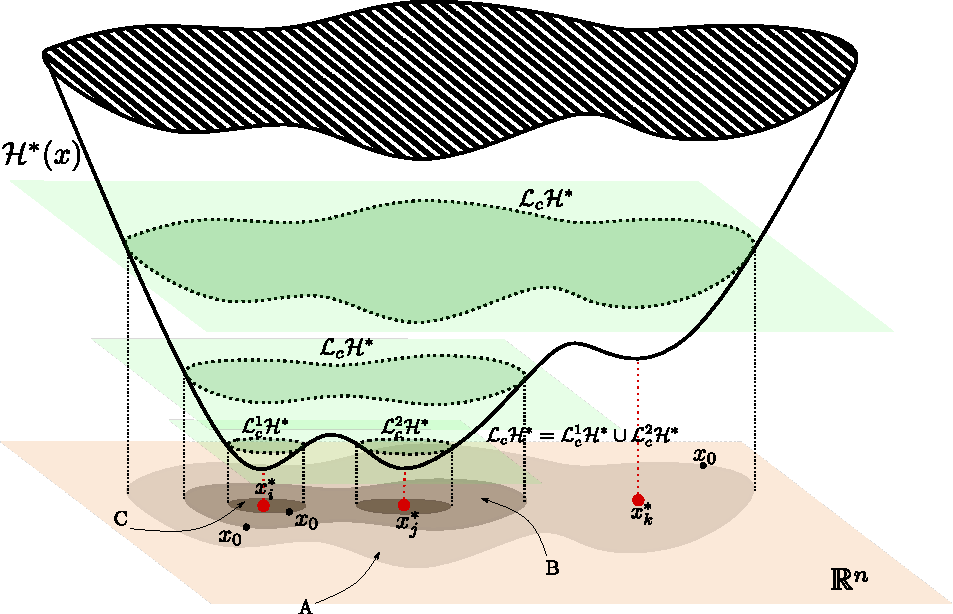
\includegraphics[scale = 0.5]{draw3.pdf}
%    \caption{\footnotesize Graphical representation of the necessary condition given by Theorem 5. Case (A): the condition is satisfied for all the stable fixed points $x_i^*,~x_j^*$ and $x_k^*$. Case (B): the condition is satisfied for $x_i^*,~x_j^*$ but not for $x_k^*$. Case (C): the condition is satisfied only for $x_i^*$.}
%    \label{fig:nec}
%\end{figure}
%}
In order to choose among the possibly infinite values of $\kappa$ such that  $x_0\in\mathcal{B}_i$, one could minimise the damping injection control effort needed to bring $x(t)$ from $x_0$ to $x_i^*$, i.e.,
\[\min_\kappa\int_0^\infty \kappa^2x^\top(s)PBB^\top Px(s)ds\]
This optimisation problem can be simply solved by minimising $\kappa$ such that $x_0\in\mathcal{B}_i(\kappa)$  
\begin{equation*}
\begin{aligned}
& \underset{\kappa}{\text{minimize}}
& & \kappa \\
& \text{subject to}
& &\lim\limits_{t\rightarrow\infty}\Phi(t,x_0,\beta(x)-\kappa B^\top Px)=x^*_i
\end{aligned}
\end{equation*}
This strategy indeed minimises the damping injection control effort but, however, inevitably leads to long transient behaviours depending on the natural dissipation of the system $x^\top PA x$.

Instead, it would be possible to choose on optimal value of $\kappa$ which instead minimises the approaching time to the desired fixed point, i.e., by solving the constrained optimisation problem:
%
\begin{equation*}
\begin{aligned}
& \underset{\kappa}{\text{minimize}}
& & t_a \\
& \text{subject to}
& & \left\{
\begin{matrix*}
\lim\limits_{t\rightarrow\infty}\Phi(t,x_0,\beta(x)-\kappa PBx)=x^*_i\\
\Phi(t_a,x_0,\beta(x)-\kappa PBx)\in\delta_\rho x_i^*
\end{matrix*}
\right.
\end{aligned}
\end{equation*}
%
where $\delta_\rho x^*_i$ is an open neighborhood of $x_i^*$ of radius $\rho$.

Note that the two optimisation problems mentioned above can be easily solved with any numerical algorithm by approximating the constraints as
\begin{align*}
    \lim\limits_{t\rightarrow\infty}&\Phi(t,x_0,\beta(x)-\kappa PBx)=x^*_i\\    
    &\Rightarrow \|\hat{\Phi}(T,x_0,\beta(x)-\kappa PBx)-x^*_i\|_2\leq\varepsilon
\end{align*}
%
where $\hat{\Phi}$ is the numerically integrated trajectory of the system, $T\gg 1$ is the integration time and $\varepsilon \ll 1$ is a chosen threshold.
Similarly,
\begin{align*}
    \Phi(t_a,&x_0,\beta(x)-kPBx)\in\delta_\rho x_i^*\\    
    &\Rightarrow \|\hat{\Phi}(t_a,x_0,\beta(x)-kPBx)-x^*_i\|_2\leq\rho
\end{align*}
}
\fi
%
%
\section{Hybrid Mode Selector}
%
Once the feedback law and the damping injection are designed to produce the desired working modes and to shape their basins of attraction, the proposed strategy aims to switch from a working mode to another.
In particular, considering the system to be in one of the working modes $\xb_i^*$, a control action which moves the system to another desired mode, $\xb_j^*$, is designed.
The strategy reckons on the following actions:
\begin{itemize}
    \item [1.] Switch-off the energy shaping controller (the system turns back linear);
    \item [2.] Give an impulse to the system to bring the state inside the basin of attraction of $\xb_j^*$;
    \item [3.] Switch on again the energy shaping controller.
\end{itemize}
%
\subsection{Impulse generation}
When the nonlinear controller $\ub=\bm\beta(\xb)+\vb$ is switched off, i.e. $\ub=\mymathbb{0}_m$, the system turns back in the LTI form (\ref{eq:lsys}).
Without loss of generality, let $t = 0$ and let the LTI system be controllable. The response of the system to a weighted impulse input 
%
\begin{equation}
\ub(t) = \bm\nu\delta(t)
\end{equation}
%
where $\bm\nu\in\R^m$ distributes the Dirac delta function $\delta(t)$ among the $m$ inputs,
is
%
\begin{align}\label{eq:impresp}
    \xb(t) &= e^{t\Ab}\xb_0 + \int_0^te^{(t-s)\Ab}\Bb \ub(s)ds =\nonumber\\
    &= e^{t\Ab}\xb_0 + \int_0^te^{(t-s)\Ab}\Bb\bm\nu\delta(s)ds \nonumber\\
    &= e^{t\Ab}\xb_0 + e^{t\Ab}\Bb\bm\nu\\
    &= e^{t\Ab}\left(\xb_0 + \Bb\bm\nu\right) .
\end{align}
%
Since the control objective is to move the system from $\xb_i^*$ to $\xb_j^*$ in a time $t^*$, it is tempting to impose the desired behaviour in (\ref{eq:impresp}) by requiring:
%
\begin{equation}\label{eq:cond}
    \xb_j^* \triangleq \xb(t^*) = e^{t^*\Ab}\left(\xb_i^* + \Bb\bm\nu\right).
\end{equation}
%
Therefore, $\bm\nu$ might be obtained as
\begin{align}
    \bm\nu = \left(\Bb^\top\Bb\right)^{-1}\Bb^\top(e^{-t^*\Ab}\xb_j^*-\xb_i^*).
\end{align}
%
However, unless $m = n$, (\ref{eq:cond}) is overdetermined, i.e. $n$ (scalar) equations with only $m$ unknowns (the components of $\bm\nu$). 
To overcome this issue, the design of the impulse controller is achieved by solving the following optimisation problem: 
find $t^*$, $\bm\nu$ such that 
%
\begin{equation}\label{eq:opti}
\begin{aligned}
& [t^*,\bm\nu] = \argmin\limits_{t^*,\bm\nu}\gamma\left\|\bm\nu \right\|^2_2+\rho\left\|\xb_j^* - e^{t^*\Ab}\left(\xb_i^*+\Bb\bm\nu\right)\right\|^2_2\\
& \text{subject to} ~~\bm\varphi\left(t^*,\xb_i^*,\bm\nu\delta(t)\right)\in\B_j
\end{aligned}
\end{equation}
where $\gamma,~\rho\in \R^+$ are two arbitrary weights and  $\B_j$ is the basin of attraction of $\xb_j^*$. 
The term $\gamma\|\bm\nu\|_2^2$ has been introduce for regularization since, in some cases, it might be convenient to simultaneously minimise also the squared norm of the impulse weights.
%

The solution of (\ref{eq:opti}), provides an impulsive input  $\ub = \bm\nu\delta$ which guarantee that the system will arrive in $\B_j$ in a time $t^*$.  
For the sake of a latter numerical implementation, the constraint was defined as
\begin{align}
    \left\|\hat{\bm\varphi}\left(t_{\infty},e^{t^*\Ab}\left(\xb_i^*+\Bb\bm\nu\right),\bm\beta(\xb)-\mathbf{K}_d\Bb^\top \Pb\xb\right)-\xb^*_j\right\|_2\leq\varepsilon
\end{align}
%
where $\hat{\bm\varphi}$ is the numerically integrated trajectory of the system, $t_\infty\gg 1$ is the integration time and $0\leq\varepsilon \ll 1$ is a chosen threshold.
%
\begin{rem}
	Assuming that the switch is performed only at steady--state, the optimisation of $\bm\nu$ and $t^*$ for each pair of fixed points $\xb_i$, $\xb_j$ can be performed off--line.
\end{rem}
%
%%%%%%%%%%%%%%%%%%%%%%%%%%%%%%%%%
\subsection{Overall Hybrid System}
%
If an impulse is applied to the system at time $t$  in order to reach the desired destination $\xb_j^*$, in the instant of time in which the impulse is applied, the state undergoes to a discontinuous jump
%
\begin{equation}\label{eq:jump}
    \xb^+ = \xb(t) + \Bb\bm\nu.
\end{equation}
%
Therefore, the controlled system can be described as an \textit{hybrid automata}, with two logic states $\Sa_1$ and $\Sa_2$. In $\Sa_1$ the system is controlled with the multistable EB--PBC and in $\Sa_2$ the system is completely uncontrolled. Thus, by introducing a timer $\tau$ and an external asynchronous signal $r$ (initialised to $0$), the transition from $\Sa_1$ to $\Sa_2$ will happen when $r$ changes from $0$ to the index of the desired fixed point, i.e., $r\in\{0,1,\dots,p\}$, with a state jump described by (\ref{eq:jump}) and resetting the timer $\tau$ to $0$. Then the system will remain uncontrolled (and thus linear) for a time $t^*$, i.e. $\tau = t^*$ after which the logic state will switch back from $\Sa_2$ to $\Sa_1$  and the timer and the external signal $r$ will be reset. A graphical representation of the designed hybrid automata is given in Fig. \ref{fig:automata}. 
%
\begin{figure}[h]
	\centering
	\scalebox{0.9}{
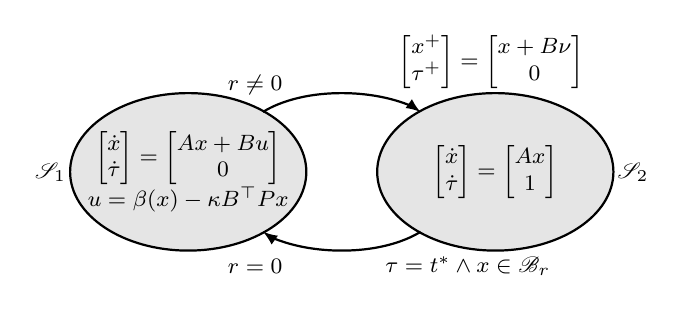
\begin{tikzpicture}
	\footnotesize
	%
	% 
	\fill[gray!20, draw = black,thick] (-1.95,0) ellipse (1.5cm and 1cm);
	\fill[gray!20, draw = black,thick] (1.95,0) ellipse (1.5cm and 1cm);
	%	
	\draw (-1.95,0) node[align = center](flow)  {$\begin{bmatrix}
\dot{x}\\\dot{\tau}\end{bmatrix} = \begin{bmatrix}Ax+Bu\\0\end{bmatrix}$\\$u = \beta(x)-\kappa B^\top Px$};
	\draw (1.95,0) node[align = center](flow)  {$\begin{bmatrix}
\dot{x}\\\dot{\tau}\end{bmatrix} = \begin{bmatrix}Ax\\1\end{bmatrix}$};
	%
	\draw [thick,-latex] plot [smooth, tension=1.2] coordinates { (-1,0.76) (0,1) (1,0.76)};
	\draw [thick,-latex] plot [smooth, tension=1.2] coordinates { (1,-0.76) (0,-1) (-1,-0.76)};
	%
	\draw (1.9,1.4) node {$\begin{bmatrix}x^+\\\tau^+\end{bmatrix} = \begin{bmatrix}x+B\nu\\0\end{bmatrix}$};
	\draw (1.6,-1.2) node {$\tau = t^*\land x\in\mathcal{B}_r$};
	%
	%
	%\draw (-1.9,-1.1) node {$\omega^+ = \nu_{w}(x,\omega)$};
	\draw (-1.1,1.1) node {$r \neq 0$};
	\draw (-1.1,-1.2) node {$r = 0$};
	\draw (-3.7,0) node {$\mathcal{S}_1$};
	\draw (3.7,0) node {$\mathcal{S}_2$};
	%
	\end{tikzpicture}}
	\caption{Hybrid automata representing the overall controlled system with the hybrid mode selector.}
	\label{fig:automata}
\end{figure}
%
\clearpage
%%%%%%%%%%%%%%%%%%%%%%%%%%%%%%%%%%%%%%%%%%%%%%%%%%%%%%%%%%%%%%%%%%%%%%%%%%%%%%%%%%%%%%%%%%%%%%%%
\section{Hybrid Port--Hamiltonian Model and Stability}
%
From the hybrid automata representation of Fig. \ref{fig:automata} the extended hybrid port--Hamiltonian model can be obtained. First, the system has two PH flows: one when the system is controlled via multistable EB-PBC
%
\begin{equation}
    \dot{\xb} = \Ab\Pb^{-1}\bm\nabla\Ha_1(\xb) + \Bb\vb
\end{equation}
%
and one when the controller is switched-off
%
\begin{equation}
    \dot{\xb} = \Ab\Pb^{-1}\bm\nabla\Ha_2(\xb)
\end{equation}
%
By introducing a dummy variable $s$, representing the logic state of the system, i.e. $s = i$ in $\Sa_i$, and performing a state extension:
%
\begin{equation}
    \zb \triangleq \left(\xb, \tau,r,s\right)
\end{equation}
%
the flow set can be defined as the union of two subsets $\C_1$ and $\C_2$ corresponding to the logic states of the system, i.e.
%
\begin{equation}
    \C \triangleq \C_1\cup\C_2
\end{equation}
%
where
%
\begin{equation}
    \C_i\triangleq \{\zb: s = i\}.
\end{equation}
%
The port--Hamiltonian set--valued mapping $\F_{\tt PH}$ can be then defined as
%
\begin{equation}
48
\end{equation}
%
\clearpage
%%%%%%%%%%%%%%%%%%%%%%%%%%%%%%%%%%%%%%%%%%%%%%%%%%%%%%%%%%%%%%%%%%%%%%%%%%%%%%%%%%%%%%%%%%%%%%%%
\section{Numerical Simulation}
%
A numerical simulation of the overall controlled system has been performed to validate the proposed control scheme. The whole procedure has been implemented in the \textsc{Matlab}\textsuperscript{\textregistered}%\footnote{The source code is available at \url{https://github.com/massastrello/MultistableControl}.} 
environment. The system introduced in Example \ref{ex:msd_sys} has been controlled with the multistable energy shaping (\ref{eq:ex_ctrl}) and the damping injection $v = -\kappa\dot{\xi}$. The system parameters has been chosen as $k = 5$, $b = 0.5$ and, as in the example in Section \ref{sec:multistable}, the minima of $\Ha^*$ have been positioned in $[\pm 0.5,0]^\top$ by setting $\lambda = 2$ and $\mu = 1$.
{%\color{red}
To implement the asynchronous external control signal $r$, the two fixed points have been denoted with $\xb_1^* = [-0.5,0]^\top$ and $\xb_2^* = [0.5,0]^\top$.}
The dissipation rate $k_d$ has been set to $4.5$. 
The \textit{fmincon} solver of the \textit{global optimization toolbox} of \textsc{Matlab}\textsuperscript{\textregistered} has been employed to solve the optimisation problem (\ref{eq:opti}). The optimisation parameters have been chosen as $t_\infty=10^3$, $\varepsilon=10^{-5}$, considering an absolute tolerance of $10^{-6}$ for the numerical integration (ODE45).
Starting from the initial state $\xb_0 \triangleq [-0.8,0]^\top$, the system, controlled with the nonlinear state feedback and the damping injection, has been integrated until secured convergence to $\xb_1^*$ ($5s$). Then, $r$ has been set to 2 in order to trigger the change of working mode, i.e. to bring the state to $\xb_2^*$. After the jump, the system has been let flowing uncontrolled for a time $t^*$ and then the nonlinear controller has been turned on again. After other $5s$ the procedure has been repeated, by setting $r$ to 1 and bring the state back in $\xb_1^*$.
This simulation has been performed twice, with different values of $\gamma$ for the impulse design process (performed off--line); $\rho$ has been set to 1 in both cases. 

First, $\gamma$ has been set to $10^{-3}$ to emphasise the minimisation of the norm of the error 
%
\begin{equation}
    \|\mathbf{e}\|_2^2=\left\|\xb_j^* - e^{t^*\Ab}\left(\xb_i^*+\Bb\bm\nu\right)\right\|^2_2.
\end{equation}
%
Then, $\gamma$ has been set to 2, accentuating the minimisation of the squared norm $\|\bm\nu\|_2^2$ of the impulse weights vector (in this case $\nu\in\R$). The numerical results of the optimisation are reported in Table \ref{tab:opti} while the system trajectories are shown in Figs. \ref{fig:exp1} and \ref{fig:exp2}. In the first case ($\gamma = 10^{-3}$), the transient from $\xb_1^*$ to $\xb_2^*$ (and vice versa) is very fast and without any oscillation in the displacement, due to the high dissipation rate and the minimised error norm: when the EB--PBC controller is switched--on again the state is very close to the desired energy minimum. However, the price of this performance is the impulse, i.e. state jump, that has to be generated. On the other hand, when $\gamma = 2$, no state discontinuity is needed to change working mode, but at the cost of a slower transient.
%
\begin{table}[h]
    \caption{Hybrid controller optimisation results.}
	\centering
	\subtable[$1^{\text{st}}$ impulse ($x_1^*\rightarrow \B_2$)]{
		\begin{tabular}{|c|c|c|c|}\hline
			\rowcolor{gray!50} $\gamma$ & $\|e\|_2^2$ &$\nu$  & $t^*$  \\\hline
            $10^{-3}$  & 0.00 & 1.05 & 1.04 \\\hline
			$2$      & 0.15 & 0.00      & 1.41 \\\hline
		\end{tabular}
	}
	\subtable[$2^{\text{nd}}$ impulse ($x_2^*\rightarrow \B_1$)]{
		%\centering
		\begin{tabular}{|c|c|c|c|}\hline
			\rowcolor{gray!50} $\gamma$ & $\|e\|_2^2$ & $\nu$  & $t^*$   \\\hline
            $10^{-3}$ & 0.00 & 1.05 & -1.05 \\\hline
			$2$      & 0.15 & 0.00      & 1.42  \\\hline
		\end{tabular}
	} 
	\label{tab:opti}
\end{table}	
%
%
%
%{\color{red}
%performing a state extension $z = [x,\xi]^\top$, the behavior 
%Notice that the resulting hybrid system can be modeled as the following \textit{hybrid inclusion} (see \cite{4806347}) 
%%
%\begin{equation}
%    \left\{
%    \begin{matrix*}[l]
%        \begin{bmatrix}
%        \dot{x}\\\dot{\xi}
%        \end{bmatrix}\in F && \begin{bmatrix}
%        {x}\\\xi
%        \end{bmatrix}\in\C
%        \\\\
%        \begin{bmatrix}
%        {x}^+\\\xi^+
%        \end{bmatrix}\in G && \begin{bmatrix}
%        {x}\\\xi
%        \end{bmatrix}\in\D
%    \end{matrix*}
%    \right.
%\end{equation}
%%
%where 
%\begin{align*}
%    \C &\triangleq \C_1\cup\C_2 \\
%       & = \{x,\xi|x\in\X \land \xi = 0\land r = 0\}\\
%       &\quad\cup\{x,\xi|x\in\X\land0\leq \xi\leq t^* \land r \neq 0\}
%\end{align*}
%%
%%and 
%%
%\begin{align*}
%    \D &\triangleq \D_1\cup\D_2 \\
%       & = \{x,\xi|x\in \X \land \xi = 0\land r \neq 0\}\\
%       &\quad\cup\{x,\xi|x\in\X \land \xi =  t^*\}
%\end{align*}
%%
%\begin{align*}
%    F &\triangleq F_1\cup F_2 \\
%       & = \{[Ax + Bu,0]^\top \land[x,\xi]^\top\in \C_1\}\\
%       &\quad\cup\{[Ax,1]^\top \land [x,\xi]^\top\in\C_2\}
%\end{align*}
%%
%\begin{align*}
%    G &\triangleq G_1\cup G_2 \\
%       & = \{[x+B\nu,0]^\top \land[x,\xi]^\top\in \D_1\}\\
%       &\quad\cup\{[0,0]^\top \land [x,\xi]^\top\in\D_2\}
%\end{align*}
%}
%
%
%\begin{figure}
%    \centering
%    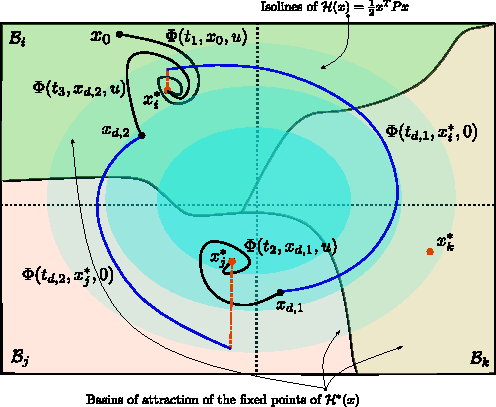
\includegraphics[scale = 1]{draw.pdf}
%    \caption{\footnotesize Graphical representation of a state-space trajectory of the controlled system.}
%    \label{fig:my_label}
%\end{figure}
%%%%
%\section{Case of Study}
%
\begin{figure}[h]
    \centering
    %\subfigure[{\footnotesize Time evolution of the states $x = [\xi,\dot{\xi}]^\top$.}]{%%
\definecolor{ocean}{rgb}{0.00000,0.44700,0.74100}
%
\begin{tikzpicture}

\begin{axis}[%
width=11cm,
height=2cm,
at={(0.758in,1.9in)},
scale only axis,
xmin=0,
xmax=17,
xlabel style={font=\color{white!15!black}},
xlabel={$t$ [$s$]},
ymin=-.8,
ymax=0.75,
ylabel style={font=\color{white!15!black}},
ylabel={$q(t)$ [m]},
axis background/.style={fill=white},
legend style={legend cell align=left, align=left, draw=white!15!black}
]
\addplot [color=ocean, dashed, line width=1.0pt,forget plot]
  table[row sep=crcr]{%
0	0.5\\
17.103	0.5\\
};
%\addlegendentry{data1}

\addplot [color=ocean, dashed, line width=1.0pt,forget plot]
  table[row sep=crcr]{%
0	-0.5\\
17.103	-0.5\\
};
%\addlegendentry{data2}

\addplot [color=black, line width=2pt]
  table[row sep=crcr]{%
0	-0.8\\
0.0201272951242755	-0.79951111951868\\
0.040254590248551	-0.79811008082095\\
0.0603818853728264	-0.795891468826249\\
0.0805091804971019	-0.792944776187467\\
0.141450272956506	-0.780417561508645\\
0.20239136541591	-0.764029602799776\\
0.263332457875313	-0.745456884813622\\
0.324273550334717	-0.725973531204578\\
0.406594062839508	-0.69990596289271\\
0.488914575344299	-0.675182591346937\\
0.571235087849089	-0.652469688739267\\
0.65355560035388	-0.632345559216368\\
0.723870856097015	-0.617338757000783\\
0.79418611184015	-0.604082781999283\\
0.864501367583285	-0.592424562970695\\
0.93481662332642	-0.582229375736837\\
1.0247788223884	-0.571064115086853\\
1.11474102145038	-0.561683876754374\\
1.20470322051236	-0.553799404485863\\
1.29466541957433	-0.547142777898694\\
1.41966541957433	-0.539436820468652\\
1.54466541957433	-0.533271711347302\\
1.66966541957433	-0.528402657479605\\
1.79466541957433	-0.524404342745406\\
1.91302238550665	-0.521127077977175\\
2.03137935143897	-0.518368646475493\\
2.14973631737129	-0.516056201969089\\
2.26809328330361	-0.514075304343261\\
2.39309328330361	-0.512245794028465\\
2.51809328330361	-0.510679923857475\\
2.64309328330361	-0.509344153381082\\
2.76809328330361	-0.508187986884424\\
2.89309328330361	-0.507171843510017\\
3.01809328330361	-0.506289351619222\\
3.14309328330361	-0.505524109227117\\
3.26809328330361	-0.504855709483334\\
3.39309328330361	-0.504267478547139\\
3.51809328330361	-0.503752835833422\\
3.64309328330361	-0.503302933885505\\
3.76809328330361	-0.502908156125825\\
3.89309328330361	-0.502560388348614\\
4.01809328330361	-0.502254970332233\\
4.14309328330361	-0.501986874345041\\
4.26809328330361	-0.501751052269233\\
4.39309328330361	-0.501543159535206\\
4.51809328330361	-0.501360211144487\\
4.64309328330361	-0.501199269031116\\
4.76809328330361	-0.501057509775478\\
4.82606996247771	-0.500997563859026\\
4.88404664165181	-0.500941038274212\\
4.9420233208259	-0.500887735750696\\
5	-0.500837469394745\\
};
%\addlegendentry{data3}

\addplot [color=gray, line width=2pt]
  table[row sep=crcr]{%
5	-0.500837469394745\\
5.001	-0.49979049724748\\
5.002	-0.498741550128628\\
5.003	-0.497690634268849\\
5.004	-0.496637755905533\\
5.005	-0.495582921282759\\
5.006	-0.494526136651266\\
5.007	-0.493467408268413\\
5.008	-0.492406742398151\\
5.009	-0.491344145310982\\
5.01	-0.490279623283929\\
5.011	-0.489213182600499\\
5.012	-0.488144829550648\\
5.013	-0.487074570430748\\
5.014	-0.486002411543552\\
5.015	-0.484928359198159\\
5.016	-0.483852419709978\\
5.017	-0.482774599400694\\
5.018	-0.481694904598237\\
5.019	-0.48061334163674\\
5.02	-0.47952991685651\\
5.021	-0.478444636603992\\
5.022	-0.477357507231732\\
5.023	-0.476268535098345\\
5.024	-0.475177726568479\\
5.025	-0.47408508801278\\
5.026	-0.472990625807857\\
5.027	-0.471894346336247\\
5.028	-0.470796255986381\\
5.029	-0.46969636115255\\
5.03	-0.468594668234867\\
5.031	-0.467491183639235\\
5.032	-0.46638591377731\\
5.033	-0.465278865066468\\
5.034	-0.464170043929769\\
5.035	-0.463059456795921\\
5.036	-0.461947110099249\\
5.037	-0.460833010279654\\
5.038	-0.459717163782583\\
5.039	-0.458599577058993\\
5.04	-0.457480256565313\\
5.041	-0.456359208763413\\
5.042	-0.455236440120568\\
5.043	-0.454111957109419\\
5.044	-0.452985766207944\\
5.045	-0.45185787389942\\
5.046	-0.450728286672388\\
5.047	-0.449597011020615\\
5.048	-0.448464053443067\\
5.049	-0.447329420443865\\
5.05	-0.446193118532255\\
5.051	-0.445055154222572\\
5.052	-0.443915534034204\\
5.053	-0.442774264491558\\
5.054	-0.441631352124023\\
5.055	-0.440486803465939\\
5.056	-0.439340625056556\\
5.057	-0.438192823440002\\
5.058	-0.437043405165252\\
5.059	-0.435892376786083\\
5.06	-0.434739744861047\\
5.061	-0.433585515953434\\
5.062	-0.432429696631236\\
5.063	-0.43127229346711\\
5.064	-0.430113313038346\\
5.065	-0.42895276192683\\
5.066	-0.427790646719011\\
5.067	-0.426626974005863\\
5.068	-0.42546175038285\\
5.069	-0.424294982449892\\
5.07	-0.423126676811331\\
5.071	-0.421956840075892\\
5.072	-0.420785478856653\\
5.073	-0.419612599771004\\
5.074	-0.418438209440616\\
5.075	-0.417262314491403\\
5.076	-0.416084921553491\\
5.077	-0.414906037261176\\
5.078	-0.413725668252895\\
5.079	-0.412543821171189\\
5.08	-0.411360502662664\\
5.081	-0.410175719377961\\
5.082	-0.40898947797172\\
5.083	-0.407801785102539\\
5.084	-0.406612647432948\\
5.085	-0.405422071629365\\
5.086	-0.404230064362065\\
5.087	-0.403036632305147\\
5.088	-0.401841782136493\\
5.089	-0.400645520537737\\
5.09	-0.399447854194227\\
5.091	-0.398248789794994\\
5.092	-0.39704833403271\\
5.093	-0.39584649360366\\
5.094	-0.394643275207702\\
5.095	-0.393438685548233\\
5.096	-0.392232731332152\\
5.097	-0.391025419269831\\
5.098	-0.389816756075069\\
5.099	-0.388606748465069\\
5.1	-0.387395403160393\\
5.101	-0.38618272688493\\
5.102	-0.384968726365864\\
5.103	-0.383753408333633\\
5.104	-0.382536779521899\\
5.105	-0.381318846667507\\
5.106	-0.380099616510457\\
5.107	-0.378879095793861\\
5.108	-0.377657291263914\\
5.109	-0.376434209669855\\
5.11	-0.375209857763933\\
5.111	-0.373984242301372\\
5.112	-0.372757370040337\\
5.113	-0.371529247741893\\
5.114	-0.370299882169979\\
5.115	-0.369069280091363\\
5.116	-0.367837448275615\\
5.117	-0.366604393495067\\
5.118	-0.365370122524777\\
5.119	-0.3641346421425\\
5.12	-0.362897959128645\\
5.121	-0.361660080266244\\
5.122	-0.360421012340917\\
5.123	-0.359180762140835\\
5.124	-0.357939336456686\\
5.125	-0.35669674208164\\
5.126	-0.355452985811312\\
5.127	-0.354208074443729\\
5.128	-0.352962014779294\\
5.129	-0.35171481362075\\
5.13	-0.350466477773145\\
5.131	-0.3492170140438\\
5.132	-0.347966429242268\\
5.133	-0.346714730180303\\
5.134	-0.345461923671826\\
5.135	-0.344208016532885\\
5.136	-0.342953015581624\\
5.137	-0.341696927638246\\
5.138	-0.340439759524977\\
5.139	-0.339181518066036\\
5.14	-0.337922210087593\\
5.141	-0.336661842417738\\
5.142	-0.335400421886444\\
5.143	-0.334137955325534\\
5.144	-0.332874449568645\\
5.145	-0.331609911451192\\
5.146	-0.330344347810333\\
5.147	-0.329077765484936\\
5.148	-0.327810171315542\\
5.149	-0.32654157214433\\
5.15	-0.325271974815084\\
5.151	-0.324001386173155\\
5.152	-0.322729813065428\\
5.153	-0.321457262340287\\
5.154	-0.320183740847578\\
5.155	-0.318909255438578\\
5.156	-0.317633812965955\\
5.157	-0.316357420283737\\
5.158	-0.315080084247277\\
5.159	-0.313801811713214\\
5.16	-0.312522609539442\\
5.161	-0.311242484585075\\
5.162	-0.30996144371041\\
5.163	-0.308679493776893\\
5.164	-0.307396641647085\\
5.165	-0.306112894184626\\
5.166	-0.3048282582542\\
5.167	-0.303542740721503\\
5.168	-0.302256348453202\\
5.169	-0.300969088316908\\
5.17	-0.299680967181136\\
5.171	-0.29839199191527\\
5.172	-0.297102169389532\\
5.173	-0.295811506474943\\
5.174	-0.294520010043293\\
5.175	-0.293227686967099\\
5.176	-0.29193454411958\\
5.177	-0.290640588374614\\
5.178	-0.289345826606706\\
5.179	-0.288050265690955\\
5.18	-0.286753912503019\\
5.181	-0.285456773919077\\
5.182	-0.284158856815798\\
5.183	-0.282860168070305\\
5.184	-0.281560714560141\\
5.185	-0.280260503163233\\
5.186	-0.27895954075786\\
5.187	-0.277657834222614\\
5.188	-0.276355390436372\\
5.189	-0.275052216278254\\
5.19	-0.273748318627596\\
5.191	-0.272443704363908\\
5.192	-0.271138380366845\\
5.193	-0.269832353516173\\
5.194	-0.268525630691728\\
5.195	-0.26721821877339\\
5.196	-0.265910124641041\\
5.197	-0.264601355174536\\
5.198	-0.263291917253668\\
5.199	-0.26198181775813\\
5.2	-0.260671063567484\\
5.201	-0.259359661561126\\
5.202	-0.258047618618251\\
5.203	-0.25673494161782\\
5.204	-0.255421637438523\\
5.205	-0.25410771295875\\
5.206	-0.252793175056549\\
5.207	-0.251478030609599\\
5.208	-0.250162286495173\\
5.209	-0.248845949590103\\
5.21	-0.247529026770747\\
5.211	-0.246211524912954\\
5.212	-0.244893450892031\\
5.213	-0.243574811582708\\
5.214	-0.242255613859104\\
5.215	-0.240935864594694\\
5.216	-0.239615570662274\\
5.217	-0.238294738933926\\
5.218	-0.236973376280986\\
5.219	-0.23565148957401\\
5.22	-0.234329085682737\\
5.221	-0.233006171476058\\
5.222	-0.231682753821984\\
5.223	-0.230358839587605\\
5.224	-0.229034435639065\\
5.225	-0.22770954884152\\
5.226	-0.22638418605911\\
5.227	-0.225058354154922\\
5.228	-0.22373205999096\\
5.229	-0.222405310428105\\
5.23	-0.221078112326087\\
5.231	-0.219750472543448\\
5.232	-0.21842239793751\\
5.233	-0.217093895364341\\
5.234	-0.215764971678721\\
5.235	-0.214435633734109\\
5.236	-0.213105888382607\\
5.237	-0.21177574247493\\
5.238	-0.210445202860371\\
5.239	-0.209114276386766\\
5.24	-0.207782969900463\\
5.241	-0.206451290246286\\
5.242	-0.205119244267504\\
5.243	-0.203786838805796\\
5.244	-0.202454080701216\\
5.245	-0.201120976792166\\
5.246	-0.199787533915354\\
5.247	-0.198453758905768\\
5.248	-0.197119658596637\\
5.249	-0.195785239819401\\
5.25	-0.19445050940368\\
5.251	-0.193115474177233\\
5.252	-0.191780140965933\\
5.253	-0.19044451659373\\
5.254	-0.189108607882618\\
5.255	-0.187772421652601\\
5.256	-0.186435964721663\\
5.257	-0.185099243905732\\
5.258	-0.183762266018648\\
5.259	-0.182425037872131\\
5.26	-0.181087566275745\\
5.261	-0.179749858036868\\
5.262	-0.17841191996066\\
5.263	-0.177073758850025\\
5.264	-0.175735381505582\\
5.265	-0.174396794725634\\
5.266	-0.17305800530613\\
5.267	-0.171719020040634\\
5.268	-0.170379845720297\\
5.269	-0.169040489133817\\
5.27	-0.16770095706741\\
5.271	-0.166361256304778\\
5.272	-0.165021393627074\\
5.273	-0.163681375812872\\
5.274	-0.162341209638133\\
5.275	-0.16100090187617\\
5.276	-0.159660459297622\\
5.277	-0.158319888670414\\
5.278	-0.156979196759729\\
5.279	-0.155638390327976\\
5.28	-0.154297476134753\\
5.281	-0.152956460936822\\
5.282	-0.151615351488068\\
5.283	-0.150274154539473\\
5.284	-0.148932876839083\\
5.285	-0.147591525131972\\
5.286	-0.146250106160215\\
5.287	-0.144908626662849\\
5.288	-0.14356709337585\\
5.289	-0.142225513032091\\
5.29	-0.140883892361318\\
5.291	-0.139542238090113\\
5.292	-0.138200556941864\\
5.293	-0.136858855636731\\
5.294	-0.135517140891619\\
5.295	-0.134175419420138\\
5.296	-0.13283369793258\\
5.297	-0.13149198313588\\
5.298	-0.130150281733587\\
5.299	-0.128808600425834\\
5.3	-0.127466945909303\\
5.301	-0.126125324877194\\
5.302	-0.124783744019195\\
5.303	-0.123442210021449\\
5.304	-0.122100729566522\\
5.305	-0.120759309333373\\
5.306	-0.119417955997319\\
5.307	-0.118076676230009\\
5.308	-0.116735476699386\\
5.309	-0.115394364069661\\
5.31	-0.114053345001279\\
5.311	-0.112712426150887\\
5.312	-0.111371614171304\\
5.313	-0.11003091571149\\
5.314	-0.108690337416512\\
5.315	-0.107349885927518\\
5.316	-0.106009567881698\\
5.317	-0.104669389912261\\
5.318	-0.103329358648398\\
5.319	-0.101989480715252\\
5.32	-0.100649762733891\\
5.321	-0.0993102113212709\\
5.322	-0.0979708330902083\\
5.323	-0.0966316346493487\\
5.324	-0.095292622603135\\
5.325	-0.0939538035517772\\
5.326	-0.0926151840912212\\
5.327	-0.091276770813118\\
5.328	-0.089938570304793\\
5.329	-0.0886005891492154\\
5.33	-0.0872628339249669\\
5.331	-0.0859253112062114\\
5.332	-0.0845880275626645\\
5.333	-0.0832509895595626\\
5.334	-0.0819142037576322\\
5.335	-0.0805776767130602\\
5.336	-0.0792414149774617\\
5.337	-0.0779054250978517\\
5.338	-0.0765697136166129\\
5.339	-0.075234287071466\\
5.34	-0.07389915199544\\
5.341	-0.0725643149168403\\
5.342	-0.07122978235922\\
5.343	-0.0698955608413485\\
5.344	-0.0685616568771824\\
5.345	-0.0672280769758344\\
5.346	-0.0658948276415436\\
5.347	-0.0645619153736455\\
5.348	-0.0632293466665414\\
5.349	-0.0618971280096696\\
5.35	-0.060565265887474\\
5.351	-0.0592337667793751\\
5.352	-0.05790263715974\\
5.353	-0.0565718834978522\\
5.354	-0.0552415122578822\\
5.355	-0.0539115298988578\\
5.356	-0.0525819428746338\\
5.357	-0.0512527576338628\\
5.358	-0.0499239806199655\\
5.359	-0.0485956182711013\\
5.36	-0.047267677020138\\
5.361	-0.0459401632946234\\
5.362	-0.0446130835167548\\
5.363	-0.0432864441033503\\
5.364	-0.0419602514658187\\
5.365	-0.0406345120101312\\
5.366	-0.039309232136791\\
5.367	-0.0379844182408046\\
5.368	-0.0366600767116525\\
5.369	-0.0353362139332602\\
5.37	-0.0340128362839687\\
5.371	-0.0326899501365054\\
5.372	-0.0313675618579557\\
5.373	-0.0300456778097334\\
5.374	-0.0287243043475516\\
5.375	-0.0274034478213942\\
5.376	-0.0260831145754869\\
5.377	-0.0247633109482682\\
5.378	-0.0234440432723611\\
5.379	-0.0221253178745435\\
5.38	-0.0208071410757205\\
5.381	-0.0194895191908947\\
5.382	-0.0181724585291384\\
5.383	-0.016855965393565\\
5.384	-0.0155400460812999\\
5.385	-0.0142247068834518\\
5.386	-0.0129099540850861\\
5.387	-0.0115957939651936\\
5.388	-0.0102822327966659\\
5.389	-0.00896927684626214\\
5.39	-0.00765693237458575\\
5.391	-0.0063452056360531\\
5.392	-0.00503410287886636\\
5.393	-0.00372363034498555\\
5.394	-0.00241379427009969\\
5.395	-0.0011046008835993\\
5.396	0.000203943591451302\\
5.397	0.0015118329383424\\
5.398	0.00281906094674719\\
5.399	0.00412562141274814\\
5.4	0.00543150813886684\\
5.401	0.00673671493408997\\
5.402	0.00804123561389757\\
5.403	0.00934506400029216\\
5.404	0.0106481939218239\\
5.405	0.0119506192136194\\
5.406	0.0132523337174095\\
5.407	0.0145533312815565\\
5.408	0.0158536057610819\\
5.409	0.0171531510176924\\
5.41	0.0184519609198095\\
5.411	0.0197500293425944\\
5.412	0.0210473501679772\\
5.413	0.0223439172846833\\
5.414	0.0236397245882604\\
5.415	0.0249347659811057\\
5.416	0.0262290353724928\\
5.417	0.0275225266785995\\
5.418	0.0288152338225342\\
5.419	0.0301071507343621\\
5.42	0.0313982713511336\\
5.421	0.0326885896169101\\
5.422	0.0339780994827902\\
5.423	0.0352667949069385\\
5.424	0.0365546698546095\\
5.425	0.0378417182981771\\
5.426	0.0391279342171583\\
5.427	0.0404133115982428\\
5.428	0.0416978444353165\\
5.429	0.0429815267294897\\
5.43	0.0442643524891232\\
5.431	0.0455463157298544\\
5.432	0.0468274104746235\\
5.433	0.0481076307537001\\
5.434	0.049386970604709\\
5.435	0.0506654240726563\\
5.436	0.0519429852099562\\
5.437	0.0532196480764561\\
5.438	0.0544954067394627\\
5.439	0.055770255273769\\
5.44	0.0570441877616786\\
5.441	0.0583171982930327\\
5.442	0.0595892809652352\\
5.443	0.0608604298832792\\
5.444	0.0621306391597711\\
5.445	0.0633999029149586\\
5.446	0.064668215276754\\
5.447	0.0659355703807614\\
5.448	0.0672019623703011\\
5.449	0.0684673853964348\\
5.45	0.0697318336179926\\
5.451	0.0709953012015971\\
5.452	0.0722577823216878\\
5.453	0.0735192711605486\\
5.454	0.0747797619083308\\
5.455	0.0760392487630796\\
5.456	0.0772977259307582\\
5.457	0.078555187625274\\
5.458	0.0798116280685019\\
5.459	0.0810670414903111\\
5.46	0.0823214221285883\\
5.461	0.0835747642292631\\
5.462	0.0848270620463332\\
5.463	0.0860783098418888\\
5.464	0.087328501886136\\
5.465	0.0885776324574246\\
5.466	0.0898256958422682\\
5.467	0.0910726863353727\\
5.468	0.0923185982396584\\
5.469	0.093563425866285\\
5.47	0.0948071635346761\\
5.471	0.0960498055725434\\
5.472	0.0972913463159107\\
5.473	0.0985317801091379\\
5.474	0.0997711013049459\\
5.475	0.10100930426444\\
5.476	0.102246383357133\\
5.477	0.103482332960971\\
5.478	0.104717147462358\\
5.479	0.105950821256176\\
5.48	0.107183348745811\\
5.481	0.108414724343178\\
5.482	0.109644942468743\\
5.483	0.110873997551545\\
5.484	0.112101884029226\\
5.485	0.113328596348044\\
5.486	0.114554128962909\\
5.487	0.115778476337395\\
5.488	0.11700163294377\\
5.489	0.118223593263017\\
5.49	0.119444351784859\\
5.491	0.12066390300778\\
5.492	0.121882241439049\\
5.493	0.123099361594743\\
5.494	0.124315257999771\\
5.495	0.125529925187896\\
5.496	0.126743357701756\\
5.497	0.127955550092892\\
5.498	0.129166496921764\\
5.499	0.13037619275778\\
5.5	0.131584632179317\\
5.501	0.132791809773739\\
5.502	0.133997720137426\\
5.503	0.135202357875792\\
5.504	0.13640571760331\\
5.505	0.137607793943535\\
5.506	0.138808581529122\\
5.507	0.140008075001852\\
5.508	0.141206269012656\\
5.509	0.142403158221631\\
5.51	0.143598737298068\\
5.511	0.14479300092047\\
5.512	0.145985943776576\\
5.513	0.147177560563385\\
5.514	0.148367845987173\\
5.515	0.149556794763518\\
5.516	0.150744401617321\\
5.517	0.151930661282828\\
5.518	0.153115568503652\\
5.519	0.154299118032793\\
5.52	0.155481304632662\\
5.521	0.156662123075099\\
5.522	0.157841568141399\\
5.523	0.159019634622329\\
5.524	0.160196317318151\\
5.525	0.161371611038646\\
5.526	0.162545510603129\\
5.527	0.163718010840477\\
5.528	0.164889106589144\\
5.529	0.166058792697187\\
5.53	0.167227064022284\\
5.531	0.168393915431755\\
5.532	0.169559341802584\\
5.533	0.17072333802144\\
5.534	0.171885898984696\\
5.535	0.17304701959845\\
5.536	0.174206694778549\\
5.537	0.175364919450605\\
5.538	0.176521688550015\\
5.539	0.177676997021988\\
5.54	0.17883083982156\\
5.541	0.179983211913612\\
5.542	0.181134108272897\\
5.543	0.182283523884057\\
5.544	0.18343145374164\\
5.545	0.184577892850127\\
5.546	0.185722836223945\\
5.547	0.18686627888749\\
5.548	0.188008215875149\\
5.549	0.189148642231316\\
5.55	0.190287553010413\\
5.551	0.191424943276912\\
5.552	0.192560808105351\\
5.553	0.193695142580358\\
5.554	0.194827941796663\\
5.555	0.195959200859129\\
5.556	0.197088914882758\\
5.557	0.198217078992723\\
5.558	0.199343688324378\\
5.559	0.200468738023281\\
5.56	0.201592223245215\\
5.561	0.202714139156201\\
5.562	0.203834480932525\\
5.563	0.204953243760751\\
5.564	0.206070422837742\\
5.565	0.207186013370678\\
5.566	0.208300010577077\\
5.567	0.209412409684812\\
5.568	0.21052320593213\\
5.569	0.21163239456767\\
5.57	0.212739970850481\\
5.571	0.213845930050045\\
5.572	0.214950267446289\\
5.573	0.216052978329608\\
5.574	0.217154058000879\\
5.575	0.218253501771488\\
5.576	0.219351304963335\\
5.577	0.220447462908865\\
5.578	0.221541970951076\\
5.579	0.222634824443546\\
5.58	0.223726018750442\\
5.581	0.224815549246543\\
5.582	0.225903411317261\\
5.583	0.226989600358649\\
5.584	0.228074111777428\\
5.585	0.229156940991\\
5.586	0.230238083427467\\
5.587	0.231317534525649\\
5.588	0.232395289735098\\
5.589	0.23347134451612\\
5.59	0.234545694339791\\
5.591	0.235618334687971\\
5.592	0.236689261053326\\
5.593	0.237758468939342\\
5.594	0.238825953860342\\
5.595	0.239891711341507\\
5.596	0.240955736918885\\
5.597	0.242018026139418\\
5.598	0.24307857456095\\
5.599	0.244137377752249\\
5.6	0.245194431293021\\
5.601	0.246249730773929\\
5.602	0.247303271796606\\
5.603	0.248355049973677\\
5.604	0.249405060928769\\
5.605	0.250453300296532\\
5.606	0.251499763722653\\
5.607	0.252544446863876\\
5.608	0.253587345388011\\
5.609	0.254628454973957\\
5.61	0.255667771311715\\
5.611	0.256705290102405\\
5.612	0.25774100705828\\
5.613	0.258774917902744\\
5.614	0.259807018370367\\
5.615	0.260837304206902\\
5.616	0.261865771169297\\
5.617	0.262892415025715\\
5.618	0.263917231555547\\
5.619	0.264940216549428\\
5.62	0.265961365809254\\
5.621	0.266980675148193\\
5.622	0.267998140390705\\
5.623	0.269013757372557\\
5.624	0.270027521940833\\
5.625	0.271039429953955\\
5.626	0.272049477281696\\
5.627	0.273057659805193\\
5.628	0.274063973416965\\
5.629	0.275068414020926\\
5.63	0.2760709775324\\
5.631	0.277071659878137\\
5.632	0.278070456996324\\
5.633	0.279067364836606\\
5.634	0.280062379360093\\
5.635	0.281055496539382\\
5.636	0.282046712358562\\
5.637	0.28303602281324\\
5.638	0.284023423910545\\
5.639	0.285008911669149\\
5.64	0.285992482119275\\
5.641	0.286974131302718\\
5.642	0.287953855272855\\
5.643	0.288931650094657\\
5.644	0.289907511844708\\
5.645	0.290881436611215\\
5.646	0.291853420494023\\
5.647	0.292823459604628\\
5.648	0.293791550066194\\
5.649	0.294757688013559\\
5.65	0.295721869593257\\
5.651	0.296684090963527\\
5.652	0.297644348294326\\
5.653	0.298602637767343\\
5.654	0.299558955576015\\
5.655	0.300513297925534\\
5.656	0.301465661032867\\
5.657	0.302416041126763\\
5.658	0.303364434447772\\
5.659	0.304310837248251\\
5.66	0.305255245792384\\
5.661	0.306197656356188\\
5.662	0.307138065227531\\
5.663	0.308076468706143\\
5.664	0.309012863103625\\
5.665	0.309947244743469\\
5.666	0.310879609961062\\
5.667	0.311809955103704\\
5.668	0.312738276530621\\
5.669	0.313664570612971\\
5.67	0.314588833733864\\
5.671	0.315511062288367\\
5.672	0.31643125268352\\
5.673	0.31734940133835\\
5.674	0.318265504683876\\
5.675	0.319179559163128\\
5.676	0.320091561231156\\
5.677	0.321001507355039\\
5.678	0.321909394013901\\
5.679	0.322815217698921\\
5.68	0.323718974913344\\
5.681	0.32462066217249\\
5.682	0.325520276003773\\
5.683	0.326417812946704\\
5.684	0.327313269552906\\
5.685	0.328206642386125\\
5.686	0.329097928022243\\
5.687	0.329987123049284\\
5.688	0.330874224067429\\
5.689	0.331759227689028\\
5.69	0.332642130538605\\
5.691	0.333522929252875\\
5.692	0.334401620480752\\
5.693	0.335278200883359\\
5.694	0.336152667134042\\
5.695	0.337025015918374\\
5.696	0.337895243934174\\
5.697	0.338763347891508\\
5.698	0.339629324512709\\
5.699	0.340493170532378\\
5.7	0.341354882697402\\
5.701	0.34221445776696\\
5.702	0.343071892512534\\
5.703	0.343927183717916\\
5.704	0.344780328179224\\
5.705	0.345631322704907\\
5.706	0.346480164115758\\
5.707	0.34732684924492\\
5.708	0.348171374937899\\
5.709	0.349013738052571\\
5.71	0.349853935459196\\
5.711	0.35069196404042\\
5.712	0.351527820691292\\
5.713	0.352361502319268\\
5.714	0.353193005844223\\
5.715	0.354022328198461\\
5.716	0.354849466326721\\
5.717	0.355674417186187\\
5.718	0.356497177746498\\
5.719	0.357317744989758\\
5.72	0.358136115910543\\
5.721	0.358952287515908\\
5.722	0.359766256825401\\
5.723	0.360578020871066\\
5.724	0.361387576697456\\
5.725	0.362194921361639\\
5.726	0.363000051933207\\
5.727	0.363802965494285\\
5.728	0.364603659139537\\
5.729	0.36540212997618\\
5.73	0.366198375123984\\
5.731	0.366992391715286\\
5.732	0.367784176894999\\
5.733	0.368573727820614\\
5.734	0.369361041662212\\
5.735	0.370146115602472\\
5.736	0.370928946836679\\
5.737	0.371709532572729\\
5.738	0.372487870031138\\
5.739	0.373263956445052\\
5.74	0.374037789060251\\
5.741	0.374809365135159\\
5.742	0.375578681940848\\
5.743	0.376345736761051\\
5.744	0.377110526892164\\
5.745	0.377873049643254\\
5.746	0.37863330233607\\
5.747	0.379391282305045\\
5.748	0.380146986897306\\
5.749	0.38090041347268\\
5.75	0.381651559403701\\
5.751	0.382400422075617\\
5.752	0.383146998886396\\
5.753	0.383891287246733\\
5.754	0.384633284580059\\
5.755	0.385372988322542\\
5.756	0.386110395923098\\
5.757	0.386845504843397\\
5.758	0.387578312557867\\
5.759	0.388308816553701\\
5.76	0.389037014330867\\
5.761	0.389762903402108\\
5.762	0.390486481292951\\
5.763	0.391207745541714\\
5.764	0.391926693699512\\
5.765	0.392643323330258\\
5.766	0.393357632010677\\
5.767	0.394069617330303\\
5.768	0.394779276891492\\
5.769	0.395486608309423\\
5.77	0.396191609212105\\
5.771	0.396894277240381\\
5.772	0.397594610047939\\
5.773	0.398292605301307\\
5.774	0.398988260679869\\
5.775	0.399681573875865\\
5.776	0.400372542594394\\
5.777	0.401061164553424\\
5.778	0.401747437483793\\
5.779	0.402431359129217\\
5.78	0.403112927246292\\
5.781	0.4037921396045\\
5.782	0.404468993986216\\
5.783	0.405143488186709\\
5.784	0.405815620014147\\
5.785	0.406485387289603\\
5.786	0.407152787847061\\
5.787	0.407817819533417\\
5.788	0.408480480208483\\
5.789	0.409140767744997\\
5.79	0.409798680028617\\
5.791	0.410454214957939\\
5.792	0.411107370444486\\
5.793	0.411758144412723\\
5.794	0.412406534800056\\
5.795	0.413052539556839\\
5.796	0.413696156646372\\
5.797	0.414337384044912\\
5.798	0.414976219741671\\
5.799	0.415612661738822\\
5.8	0.416246708051503\\
5.801	0.416878356707818\\
5.802	0.417507605748843\\
5.803	0.41813445322863\\
5.804	0.418758897214206\\
5.805	0.419380935785579\\
5.806	0.420000567035741\\
5.807	0.420617789070672\\
5.808	0.42123260000934\\
5.809	0.421844997983709\\
5.81	0.422454981138734\\
5.811	0.423062547632372\\
5.812	0.423667695635579\\
5.813	0.424270423332316\\
5.814	0.424870728919549\\
5.815	0.425468610607256\\
5.816	0.426064066618421\\
5.817	0.426657095189046\\
5.818	0.427247694568147\\
5.819	0.427835863017759\\
5.82	0.428421598812936\\
5.821	0.429004900241757\\
5.822	0.429585765605322\\
5.823	0.430164193217762\\
5.824	0.430740181406232\\
5.825	0.43131372851092\\
5.826	0.431884832885046\\
5.827	0.432453492894861\\
5.828	0.433019706919656\\
5.829	0.433583473351754\\
5.83	0.434144790596522\\
5.831	0.434703657072361\\
5.832	0.435260071210718\\
5.833	0.435814031456081\\
5.834	0.436365536265983\\
5.835	0.436914584110999\\
5.836	0.437461173474754\\
5.837	0.438005302853919\\
5.838	0.438546970758212\\
5.839	0.439086175710403\\
5.84	0.439622916246309\\
5.841	0.440157190914799\\
5.842	0.440688998277796\\
5.843	0.441218336910272\\
5.844	0.441745205400254\\
5.845	0.44226960234882\\
5.846	0.442791526370106\\
5.847	0.443310976091298\\
5.848	0.443827950152639\\
5.849	0.444342447207426\\
5.85	0.444854465922012\\
5.851	0.445364004975806\\
5.852	0.445871063061268\\
5.853	0.44637563888392\\
5.854	0.446877731162333\\
5.855	0.447377338628137\\
5.856	0.447874460026016\\
5.857	0.448369094113709\\
5.858	0.448861239662007\\
5.859	0.449350895454759\\
5.86	0.449838060288865\\
5.861	0.450322732974279\\
5.862	0.450804912334007\\
5.863	0.451284597204107\\
5.864	0.451761786433688\\
5.865	0.45223647888491\\
5.866	0.452708673432982\\
5.867	0.453178368966162\\
5.868	0.453645564385755\\
5.869	0.454110258606113\\
5.87	0.454572450554634\\
5.871	0.45503213917176\\
5.872	0.455489323410976\\
5.873	0.455944002238809\\
5.874	0.456396174634828\\
5.875	0.456845839591638\\
5.876	0.457292996114884\\
5.877	0.457737643223247\\
5.878	0.458179779948441\\
5.879	0.458619405335215\\
5.88	0.459056518441345\\
5.881	0.459491118337643\\
5.882	0.459923204107941\\
5.883	0.460352774849102\\
5.884	0.460779829671009\\
5.885	0.461204367696568\\
5.886	0.461626388061704\\
5.887	0.46204588991536\\
5.888	0.462462872419491\\
5.889	0.462877334749068\\
5.89	0.46328927609207\\
5.891	0.463698695649484\\
5.892	0.464105592635303\\
5.893	0.464509966276521\\
5.894	0.464911815813134\\
5.895	0.465311140498133\\
5.896	0.465707939597506\\
5.897	0.46610221239023\\
5.898	0.466493958168274\\
5.899	0.46688317623659\\
5.9	0.467269865913114\\
5.901	0.467654026528761\\
5.902	0.468035657427424\\
5.903	0.468414757965968\\
5.904	0.46879132751423\\
5.905	0.469165365455011\\
5.906	0.469536871184078\\
5.907	0.469905844110155\\
5.908	0.470272283654926\\
5.909	0.470636189253026\\
5.91	0.470997560352039\\
5.911	0.471356396412494\\
5.912	0.471712696907862\\
5.913	0.472066461324554\\
5.914	0.472417689161912\\
5.915	0.472766379932209\\
5.916	0.473112533160645\\
5.917	0.47345614838534\\
5.918	0.473797225157333\\
5.919	0.474135763040577\\
5.92	0.474471761611933\\
5.921	0.474805220461166\\
5.922	0.475136139190945\\
5.923	0.475464517416832\\
5.924	0.475790354767281\\
5.925	0.476113650883633\\
5.926	0.476434405420113\\
5.927	0.476752618043821\\
5.928	0.477068288434732\\
5.929	0.477381416285687\\
5.93	0.47769200130239\\
5.931	0.478000043203407\\
5.932	0.478305541720151\\
5.933	0.478608496596888\\
5.934	0.478908907590725\\
5.935	0.479206774471605\\
5.936	0.479502097022307\\
5.937	0.479794875038434\\
5.938	0.480085108328412\\
5.939	0.480372796713482\\
5.94	0.480657940027698\\
5.941	0.480940538117917\\
5.942	0.481220590843797\\
5.943	0.481498098077788\\
5.944	0.481773059705129\\
5.945	0.482045475623841\\
5.946	0.482315345744724\\
5.947	0.482582669991343\\
5.948	0.482847448300032\\
5.949	0.483109680619882\\
5.95	0.483369366912735\\
5.951	0.48362650715318\\
5.952	0.483881101328545\\
5.953	0.484133149438894\\
5.954	0.484382651497015\\
5.955	0.484629607528419\\
5.956	0.484874017571329\\
5.957	0.485115881676677\\
5.958	0.485355199908096\\
5.959	0.485591972341914\\
5.96	0.485826199067145\\
5.961	0.486057880185485\\
5.962	0.486287015811303\\
5.963	0.486513606071637\\
5.964	0.486737651106184\\
5.965	0.486959151067293\\
5.966	0.487178106119961\\
5.967	0.487394516441822\\
5.968	0.487608382223145\\
5.969	0.487819703666818\\
5.97	0.488028480988351\\
5.971	0.488234714415862\\
5.972	0.48843840419007\\
5.973	0.488639550564291\\
5.974	0.488838153804427\\
5.975	0.489034214188958\\
5.976	0.48922773200894\\
5.977	0.489418707567988\\
5.978	0.489607141182279\\
5.979	0.489793033180533\\
5.98	0.489976383904014\\
5.981	0.490157193706518\\
5.982	0.490335462954364\\
5.983	0.490511192026391\\
5.984	0.490684381313942\\
5.985	0.490855031220863\\
5.986	0.491023142163492\\
5.987	0.491188714570647\\
5.988	0.491351748883626\\
5.989	0.491512245556191\\
5.99	0.491670205054563\\
5.991	0.49182562785741\\
5.992	0.491978514455846\\
5.993	0.492128865353413\\
5.994	0.492276681066079\\
5.995	0.492421962122226\\
5.996	0.492564709062641\\
5.997	0.492704922440511\\
5.998	0.492842602821408\\
5.999	0.492977750783285\\
6	0.493110366916464\\
6.001	0.493240451823628\\
6.002	0.493368006119813\\
6.003	0.493493030432395\\
6.004	0.493615525401086\\
6.005	0.493735491677919\\
6.006	0.493852929927244\\
6.007	0.493967840825714\\
6.008	0.494080225062277\\
6.009	0.494190083338169\\
6.01	0.494297416366901\\
6.011	0.494402224874248\\
6.012	0.494504509598247\\
6.013	0.494604271289176\\
6.014	0.494701510709554\\
6.015	0.494796228634126\\
6.016	0.494888425849852\\
6.017	0.494978103155902\\
6.018	0.495065261363642\\
6.019	0.495149901296623\\
6.02	0.495232023790576\\
6.021	0.495311629693394\\
6.022	0.49538871986513\\
6.023	0.49546329517798\\
6.024	0.495535356516275\\
6.025	0.495604904776473\\
6.026	0.495671940867145\\
6.027	0.495736465708963\\
6.028	0.495798480234697\\
6.029	0.495857985389194\\
6.03	0.495914982129376\\
6.031	0.495969471424225\\
6.032	0.49602145425477\\
6.033	0.496070931614082\\
6.034	0.496117904507258\\
6.035	0.496162373951413\\
6.036	0.496204340975667\\
6.037	0.496243806621135\\
6.038	0.496280771940915\\
6.039	0.496315238000075\\
6.04	0.496347205875648\\
6.041	0.496376676656614\\
6.042	0.496403651443891\\
6.043	0.496428131350323\\
6.044	0.49645011750067\\
6.045	0.496469611031596\\
6.046	0.496486613091655\\
6.047	0.496501124841282\\
6.048	0.496513147452781\\
6.049	0.496522682110312\\
6.05	0.496529730009879\\
6.051	0.49653429235932\\
};
%\addlegendentry{data4}

\addplot [color=black, line width=2pt]
  table[row sep=crcr]{%
6.051	0.49653429235932\\
6.176	0.496926194960609\\
6.301	0.497276850121281\\
6.426	0.497591075529191\\
6.551	0.497870227769207\\
6.676	0.498116271932668\\
6.801	0.498334587715316\\
6.926	0.498528372737258\\
7.051	0.498699911226424\\
7.176	0.498851373307831\\
7.301	0.498985372191164\\
7.426	0.499103923187673\\
7.551	0.499208710275864\\
7.676	0.499301255013317\\
7.801	0.499383029974462\\
7.926	0.499455280979485\\
8.051	0.499519098936501\\
8.176	0.499575456191341\\
8.301	0.499625225814305\\
8.426	0.49966917132255\\
8.551	0.499707973175075\\
8.676	0.499742234944969\\
8.801	0.499772482372023\\
8.926	0.499799181334092\\
9.051	0.499822750325593\\
9.176	0.499843559781005\\
9.301	0.499861927783756\\
9.426	0.499878137907887\\
9.551	0.499892445919136\\
9.676	0.49990507797607\\
9.801	0.499916226816221\\
9.926	0.499926064803327\\
10.051	0.49993474774883\\
10.176	0.499942413349355\\
10.301	0.499949178453657\\
10.426	0.499955147740769\\
10.551	0.499960415961223\\
10.676	0.499965066822313\\
10.801	0.499969171180145\\
10.926	0.499972792575672\\
11.051	0.499975988567965\\
};

%\addlegendentry{data5}

\addplot [color=gray, line width=2pt]
  table[row sep=crcr]{%
11.051	0.499975988567965\\
11.052	0.498930526268579\\
11.053	0.497883092541648\\
11.054	0.496833693608498\\
11.055	0.495782335697166\\
11.056	0.494729025042372\\
11.057	0.493673767885476\\
11.058	0.492616570474452\\
11.059	0.491557439063847\\
11.06	0.490496379914751\\
11.061	0.48943339929476\\
11.062	0.488368503477941\\
11.063	0.487301698744799\\
11.064	0.486232991382243\\
11.065	0.485162387683547\\
11.066	0.484089893948321\\
11.067	0.483015516482474\\
11.068	0.481939261598178\\
11.069	0.480861135613833\\
11.07	0.479781144854037\\
11.071	0.478699295649546\\
11.072	0.477615594337242\\
11.073	0.476530047260098\\
11.074	0.47544266076714\\
11.075	0.474353441213419\\
11.076	0.47326239495997\\
11.077	0.47216952837378\\
11.078	0.471074847827753\\
11.079	0.469978359700674\\
11.08	0.468880070377175\\
11.081	0.467779986247703\\
11.082	0.466678113708478\\
11.083	0.465574459161465\\
11.084	0.464469029014337\\
11.085	0.463361829680439\\
11.086	0.462252867578753\\
11.087	0.461142149133866\\
11.088	0.46002968077593\\
11.089	0.458915468940634\\
11.09	0.457799520069163\\
11.091	0.456681840608164\\
11.092	0.455562437009714\\
11.093	0.454441315731283\\
11.094	0.453318483235699\\
11.095	0.452193945991114\\
11.096	0.451067710470968\\
11.097	0.449939783153953\\
11.098	0.448810170523982\\
11.099	0.44767887907015\\
11.1	0.446545915286699\\
11.101	0.445411285672986\\
11.102	0.444274996733445\\
11.103	0.443137054977554\\
11.104	0.4419974669198\\
11.105	0.44085623907964\\
11.106	0.439713377981472\\
11.107	0.438568890154595\\
11.108	0.437422782133177\\
11.109	0.436275060456218\\
11.11	0.435125731667516\\
11.111	0.43397480231563\\
11.112	0.432822278953848\\
11.113	0.43166816814015\\
11.114	0.430512476437173\\
11.115	0.429355210412175\\
11.116	0.428196376637003\\
11.117	0.427035981688053\\
11.118	0.425874032146239\\
11.119	0.424710534596957\\
11.12	0.423545495630048\\
11.121	0.422378921839764\\
11.122	0.421210819824734\\
11.123	0.420041196187927\\
11.124	0.418870057536618\\
11.125	0.417697410482352\\
11.126	0.416523261640909\\
11.127	0.415347617632269\\
11.128	0.414170485080577\\
11.129	0.412991870614108\\
11.13	0.411811780865231\\
11.131	0.410630222470374\\
11.132	0.40944720206999\\
11.133	0.408262726308519\\
11.134	0.407076801834356\\
11.135	0.405889435299814\\
11.136	0.404700633361089\\
11.137	0.403510402678226\\
11.138	0.402318749915082\\
11.139	0.40112568173929\\
11.14	0.399931204822228\\
11.141	0.398735325838979\\
11.142	0.397538051468299\\
11.143	0.396339388392581\\
11.144	0.395139343297817\\
11.145	0.393937922873569\\
11.146	0.392735133812927\\
11.147	0.391530982812478\\
11.148	0.390325476572268\\
11.149	0.389118621795772\\
11.15	0.38791042518985\\
11.151	0.386700893464722\\
11.152	0.385490033333923\\
11.153	0.384277851514276\\
11.154	0.383064354725851\\
11.155	0.381849549691934\\
11.156	0.380633443138987\\
11.157	0.379416041796619\\
11.158	0.378197352397544\\
11.159	0.376977381677551\\
11.16	0.375756136375468\\
11.161	0.374533623233123\\
11.162	0.373309848995313\\
11.163	0.372084820409769\\
11.164	0.370858544227115\\
11.165	0.369631027200841\\
11.166	0.368402276087262\\
11.167	0.367172297645484\\
11.168	0.365941098637371\\
11.169	0.364708685827507\\
11.17	0.363475065983162\\
11.171	0.362240245874258\\
11.172	0.361004232273331\\
11.173	0.3597670319555\\
11.174	0.358528651698426\\
11.175	0.357289098282284\\
11.176	0.356048378489721\\
11.177	0.354806499105826\\
11.178	0.353563466918091\\
11.179	0.35231928871638\\
11.18	0.351073971292889\\
11.181	0.349827521442115\\
11.182	0.348579945960819\\
11.183	0.347331251647992\\
11.184	0.346081445304817\\
11.185	0.344830533734638\\
11.186	0.343578523742922\\
11.187	0.342325422137225\\
11.188	0.341071235727157\\
11.189	0.339815971324347\\
11.19	0.338559635742406\\
11.191	0.337302235796896\\
11.192	0.336043778305292\\
11.193	0.334784270086945\\
11.194	0.333523717963052\\
11.195	0.332262128756619\\
11.196	0.330999509292423\\
11.197	0.329735866396982\\
11.198	0.328471206898515\\
11.199	0.327205537626912\\
11.2	0.325938865413694\\
11.201	0.324671197091983\\
11.202	0.323402539496463\\
11.203	0.322132899463346\\
11.204	0.32086228383034\\
11.205	0.319590699436611\\
11.206	0.318318153122747\\
11.207	0.317044651730726\\
11.208	0.315770202103883\\
11.209	0.314494811086867\\
11.21	0.313218485525615\\
11.211	0.311941232267312\\
11.212	0.310663058160358\\
11.213	0.309383970054332\\
11.214	0.30810397479996\\
11.215	0.306823079249076\\
11.216	0.30554129025459\\
11.217	0.304258614670452\\
11.218	0.302975059351619\\
11.219	0.301690631154018\\
11.22	0.300405336934511\\
11.221	0.299119183550865\\
11.222	0.29783217786171\\
11.223	0.29654432672651\\
11.224	0.295255637005525\\
11.225	0.29396611555978\\
11.226	0.292675769251025\\
11.227	0.291384604941705\\
11.228	0.290092629494923\\
11.229	0.288799849774407\\
11.23	0.287506272644473\\
11.231	0.286211904969992\\
11.232	0.284916753616356\\
11.233	0.283620825449441\\
11.234	0.282324127335577\\
11.235	0.281026666141507\\
11.236	0.279728448734358\\
11.237	0.278429481981603\\
11.238	0.27712977275103\\
11.239	0.275829327910704\\
11.24	0.274528154328933\\
11.241	0.273226258874237\\
11.242	0.271923648415309\\
11.243	0.270620329820983\\
11.244	0.269316309960201\\
11.245	0.268011595701974\\
11.246	0.266706193915352\\
11.247	0.265400111469389\\
11.248	0.264093355233106\\
11.249	0.262785932075459\\
11.25	0.261477848865306\\
11.251	0.260169112471367\\
11.252	0.258859729762197\\
11.253	0.257549707606147\\
11.254	0.256239052871332\\
11.255	0.254927772425594\\
11.256	0.253615873136472\\
11.257	0.252303361871164\\
11.258	0.250990245496495\\
11.259	0.249676530878881\\
11.26	0.248362224884299\\
11.261	0.247047334378248\\
11.262	0.245731866225715\\
11.263	0.244415827291147\\
11.264	0.243099224438411\\
11.265	0.24178206453076\\
11.266	0.240464354430804\\
11.267	0.239146101000471\\
11.268	0.237827311100974\\
11.269	0.236507991592781\\
11.27	0.235188149335574\\
11.271	0.233867791188223\\
11.272	0.232546924008745\\
11.273	0.231225554654275\\
11.274	0.229903689981031\\
11.275	0.228581336844279\\
11.276	0.2272585020983\\
11.277	0.225935192596355\\
11.278	0.224611415190655\\
11.279	0.223287176732323\\
11.28	0.221962484071361\\
11.281	0.22063734405662\\
11.282	0.219311763535761\\
11.283	0.217985749355225\\
11.284	0.2166593083602\\
11.285	0.215332447394583\\
11.286	0.214005173300952\\
11.287	0.212677492920526\\
11.288	0.21134941309314\\
11.289	0.210020940657202\\
11.29	0.208692082449667\\
11.291	0.207362845306001\\
11.292	0.206033236060145\\
11.293	0.204703261544487\\
11.294	0.203372928589821\\
11.295	0.202042244025324\\
11.296	0.200711214678513\\
11.297	0.199379847375216\\
11.298	0.198048148939539\\
11.299	0.196716126193832\\
11.3	0.195383785958656\\
11.301	0.194051135052749\\
11.302	0.192718180292993\\
11.303	0.191384928494383\\
11.304	0.190051386469992\\
11.305	0.188717561030936\\
11.306	0.187383458986344\\
11.307	0.186049087143325\\
11.308	0.184714452306934\\
11.309	0.183379561280137\\
11.31	0.182044420863782\\
11.311	0.180709037856562\\
11.312	0.179373419054987\\
11.313	0.178037571253346\\
11.314	0.176701501243677\\
11.315	0.175365215815734\\
11.316	0.174028721756953\\
11.317	0.172692025852421\\
11.318	0.171355134884841\\
11.319	0.170018055634502\\
11.32	0.168680794879245\\
11.321	0.167343359394428\\
11.322	0.166005755952898\\
11.323	0.164667991324955\\
11.324	0.163330072278321\\
11.325	0.161992005578104\\
11.326	0.160653797986774\\
11.327	0.159315456264119\\
11.328	0.157976987167222\\
11.329	0.156638397450425\\
11.33	0.155299693865294\\
11.331	0.153960883160593\\
11.332	0.152621972082244\\
11.333	0.151282967373302\\
11.334	0.149943875773917\\
11.335	0.148604704021305\\
11.336	0.147265458849715\\
11.337	0.145926146990396\\
11.338	0.144586775171568\\
11.339	0.143247350118384\\
11.34	0.141907878552904\\
11.341	0.140568367194058\\
11.342	0.139228822757619\\
11.343	0.137889251956166\\
11.344	0.136549661499055\\
11.345	0.135210058092388\\
11.346	0.133870448438977\\
11.347	0.132530839238317\\
11.348	0.131191237186549\\
11.349	0.129851648976433\\
11.35	0.128512081297316\\
11.351	0.127172540835094\\
11.352	0.125833034272189\\
11.353	0.12449356828751\\
11.354	0.123154149556427\\
11.355	0.121814784750737\\
11.356	0.120475480538629\\
11.357	0.11913624358466\\
11.358	0.117797080549717\\
11.359	0.116457998090988\\
11.36	0.115119002861931\\
11.361	0.113780101512243\\
11.362	0.112441300687826\\
11.363	0.111102607030758\\
11.364	0.10976402717926\\
11.365	0.108425567767669\\
11.366	0.1070872354264\\
11.367	0.105749036781921\\
11.368	0.104410978456718\\
11.369	0.103073067069265\\
11.37	0.101735309233995\\
11.371	0.100397711561263\\
11.372	0.0990602806573236\\
11.373	0.097723023124293\\
11.374	0.0963859455601209\\
11.375	0.0950490545585592\\
11.376	0.0937123567091315\\
11.377	0.0923758585971018\\
11.378	0.0910395668034435\\
11.379	0.0897034879048096\\
11.38	0.0883676284735009\\
11.381	0.0870319950774362\\
11.382	0.0856965942801209\\
11.383	0.0843614326406168\\
11.384	0.0830265167135121\\
11.385	0.0816918530488891\\
11.386	0.0803574481922963\\
11.387	0.0790233086847152\\
11.388	0.0776894410625322\\
11.389	0.0763558518575067\\
11.39	0.0750225475967414\\
11.391	0.0736895348026523\\
11.392	0.0723568199929373\\
11.393	0.0710244096805474\\
11.394	0.0696923103736552\\
11.395	0.0683605285756261\\
11.396	0.0670290707849868\\
11.397	0.0656979434953965\\
11.398	0.064367153195616\\
11.399	0.0630367063694778\\
11.4	0.0617066094958568\\
11.401	0.0603768690486396\\
11.402	0.0590474914966953\\
11.403	0.057718483303845\\
11.404	0.0563898509288323\\
11.405	0.0550616008252943\\
11.406	0.0537337394417307\\
11.407	0.0524062732214745\\
11.408	0.0510792086026627\\
11.409	0.0497525520182066\\
11.41	0.0484263098957622\\
11.411	0.0471004886577005\\
11.412	0.0457750947210784\\
11.413	0.0444501344976091\\
11.414	0.0431256143936327\\
11.415	0.0418015408100865\\
11.416	0.040477920142477\\
11.417	0.0391547587808487\\
11.418	0.0378320631097566\\
11.419	0.0365098395082359\\
11.42	0.0351880943497739\\
11.421	0.0338668340022799\\
11.422	0.0325460648280565\\
11.423	0.031225793183771\\
11.424	0.0299060254204262\\
11.425	0.028586767883331\\
11.426	0.0272680269120723\\
11.427	0.0259498088404858\\
11.428	0.0246321199966268\\
11.429	0.0233149667027425\\
11.43	0.0219983552752423\\
11.431	0.0206822920246696\\
11.432	0.0193667832556733\\
11.433	0.0180518352669787\\
11.434	0.0167374543513597\\
11.435	0.0154236467956098\\
11.436	0.0141104188805134\\
11.437	0.0127977768808187\\
11.438	0.0114857270652075\\
11.439	0.0101742756962692\\
11.44	0.0088634290304692\\
11.441	0.00755319331812439\\
11.442	0.00624357480337264\\
11.443	0.00493457972414529\\
11.444	0.00362621431213956\\
11.445	0.00231848479278933\\
11.446	0.00101139738523823\\
11.447	-0.000295041697688596\\
11.448	-0.00160082624951236\\
11.449	-0.0029059500701291\\
11.45	-0.00421040696583613\\
11.451	-0.00551419074936152\\
11.452	-0.00681729523989023\\
11.453	-0.00811971426309244\\
11.454	-0.00942144165115218\\
11.455	-0.0107224712427931\\
11.456	-0.0120227968833066\\
11.457	-0.0133224124245798\\
11.458	-0.0146213117251232\\
11.459	-0.0159194886500974\\
11.46	-0.0172169370713399\\
11.461	-0.018513650867394\\
11.462	-0.0198096239235347\\
11.463	-0.0211048501317963\\
11.464	-0.0223993233910002\\
11.465	-0.0236930376067809\\
11.466	-0.0249859866916139\\
11.467	-0.0262781645648418\\
11.468	-0.0275695651527024\\
11.469	-0.0288601823883554\\
11.47	-0.030150010211908\\
11.471	-0.0314390425704433\\
11.472	-0.032727273418047\\
11.473	-0.0340146967158317\\
11.474	-0.0353013064319676\\
11.475	-0.0365870965417052\\
11.476	-0.0378720610274047\\
11.477	-0.0391561938785609\\
11.478	-0.040439489091831\\
11.479	-0.0417219406710592\\
11.48	-0.0430035426273047\\
11.481	-0.0442842889788676\\
11.482	-0.0455641737513148\\
11.483	-0.0468431909775064\\
11.484	-0.0481213346976227\\
11.485	-0.0493985989591885\\
11.486	-0.0506749778171008\\
11.487	-0.0519504653336547\\
11.488	-0.0532250555785686\\
11.489	-0.0544987426290101\\
11.49	-0.0557715205696234\\
11.491	-0.0570433834925533\\
11.492	-0.0583143254974718\\
11.493	-0.0595843406916038\\
11.494	-0.0608534231897532\\
11.495	-0.0621215671143267\\
11.496	-0.0633887665953626\\
11.497	-0.0646550157705532\\
11.498	-0.0659203087852722\\
11.499	-0.0671846397925993\\
11.5	-0.0684480029533451\\
11.501	-0.0697103924360782\\
11.502	-0.0709718024171492\\
11.503	-0.0722322270807152\\
11.504	-0.0734916606187665\\
11.505	-0.0747500972311509\\
11.506	-0.0760075311255992\\
11.507	-0.0772639565177493\\
11.508	-0.0785193676311728\\
11.509	-0.0797737586973979\\
11.51	-0.0810271239559359\\
11.511	-0.0822794576543054\\
11.512	-0.0835307540480564\\
11.513	-0.0847810074007963\\
11.514	-0.0860302119842139\\
11.515	-0.0872783620781029\\
11.516	-0.0885254519703896\\
11.517	-0.0897714759571529\\
11.518	-0.0910164283426527\\
11.519	-0.0922603034393523\\
11.52	-0.0935030955679432\\
11.521	-0.0947447990573691\\
11.522	-0.0959854082448508\\
11.523	-0.0972249174759096\\
11.524	-0.0984633211043916\\
11.525	-0.0997006134924923\\
11.526	-0.10093678901078\\
11.527	-0.10217184203822\\
11.528	-0.103405766962198\\
11.529	-0.104638558178545\\
11.53	-0.105870210091561\\
11.531	-0.107100717114037\\
11.532	-0.10833007366728\\
11.533	-0.109558274181138\\
11.534	-0.110785313094021\\
11.535	-0.112011184852926\\
11.536	-0.113235883913459\\
11.537	-0.114459404739861\\
11.538	-0.11568174180503\\
11.539	-0.116902889590543\\
11.54	-0.118122842586681\\
11.541	-0.119341595292452\\
11.542	-0.120559142215613\\
11.543	-0.121775477872694\\
11.544	-0.122990596789021\\
11.545	-0.12420449349874\\
11.546	-0.125417162544837\\
11.547	-0.126628598479163\\
11.548	-0.127838795862456\\
11.549	-0.129047749264366\\
11.55	-0.130255453263474\\
11.551	-0.131461902447319\\
11.552	-0.132667091412413\\
11.553	-0.133871014764274\\
11.554	-0.13507366711744\\
11.555	-0.136275043095497\\
11.556	-0.137475137331094\\
11.557	-0.138673944465976\\
11.558	-0.139871459150996\\
11.559	-0.141067676046144\\
11.56	-0.142262589820565\\
11.561	-0.143456195152584\\
11.562	-0.144648486729726\\
11.563	-0.14583945924874\\
11.564	-0.147029107415617\\
11.565	-0.148217425945617\\
11.566	-0.149404409563287\\
11.567	-0.150590053002484\\
11.568	-0.151774351006396\\
11.569	-0.152957298327567\\
11.57	-0.154138889727913\\
11.571	-0.155319119978747\\
11.572	-0.1564979838608\\
11.573	-0.157675476164242\\
11.574	-0.158851591688703\\
11.575	-0.160026325243296\\
11.576	-0.161199671646635\\
11.577	-0.16237162572686\\
11.578	-0.163542182321655\\
11.579	-0.164711336278271\\
11.58	-0.165879082453544\\
11.581	-0.167045415713921\\
11.582	-0.168210330935477\\
11.583	-0.169373823003936\\
11.584	-0.170535886814692\\
11.585	-0.171696517272833\\
11.586	-0.172855709293155\\
11.587	-0.174013457800189\\
11.588	-0.175169757728218\\
11.589	-0.176324604021298\\
11.59	-0.17747799163328\\
11.591	-0.178629915527827\\
11.592	-0.179780370678438\\
11.593	-0.180929352068465\\
11.594	-0.182076854691137\\
11.595	-0.183222873549575\\
11.596	-0.184367403656818\\
11.597	-0.185510440035835\\
11.598	-0.186651977719554\\
11.599	-0.187792011750876\\
11.6	-0.188930537182696\\
11.601	-0.190067549077923\\
11.602	-0.191203042509501\\
11.603	-0.192337012560426\\
11.604	-0.193469454323767\\
11.605	-0.194600362902686\\
11.606	-0.195729733410456\\
11.607	-0.196857560970482\\
11.608	-0.197983840716319\\
11.609	-0.199108567791692\\
11.61	-0.200231737350515\\
11.611	-0.20135334455691\\
11.612	-0.202473384585225\\
11.613	-0.203591852620056\\
11.614	-0.204708743856263\\
11.615	-0.205824053498991\\
11.616	-0.206937776763686\\
11.617	-0.208049908876117\\
11.618	-0.209160445072393\\
11.619	-0.210269380598982\\
11.62	-0.21137671071273\\
11.621	-0.212482430680878\\
11.622	-0.213586535781081\\
11.623	-0.214689021301429\\
11.624	-0.215789882540462\\
11.625	-0.21688911480719\\
11.626	-0.217986713421108\\
11.627	-0.219082673712223\\
11.628	-0.220176991021058\\
11.629	-0.221269660698686\\
11.63	-0.222360678106733\\
11.631	-0.223450038617409\\
11.632	-0.224537737613514\\
11.633	-0.225623770488467\\
11.634	-0.226708132646313\\
11.635	-0.22779081950175\\
11.636	-0.228871826480141\\
11.637	-0.229951149017532\\
11.638	-0.231028782560673\\
11.639	-0.23210472256703\\
11.64	-0.233178964504806\\
11.641	-0.23425150385296\\
11.642	-0.23532233610122\\
11.643	-0.236391456750101\\
11.644	-0.237458861310923\\
11.645	-0.238524545305831\\
11.646	-0.239588504267805\\
11.647	-0.240650733740685\\
11.648	-0.241711229279181\\
11.649	-0.242769986448893\\
11.65	-0.243827000826328\\
11.651	-0.244882267998916\\
11.652	-0.245935783565026\\
11.653	-0.246987543133983\\
11.654	-0.248037542326085\\
11.655	-0.24908577677262\\
11.656	-0.250132242115879\\
11.657	-0.251176934009177\\
11.658	-0.252219848116864\\
11.659	-0.253260980114348\\
11.66	-0.254300325688102\\
11.661	-0.25533788053569\\
11.662	-0.256373640365776\\
11.663	-0.25740760089814\\
11.664	-0.2584397578637\\
11.665	-0.259470107004519\\
11.666	-0.26049864407383\\
11.667	-0.261525364836042\\
11.668	-0.262550265066765\\
11.669	-0.263573340552819\\
11.67	-0.26459458709225\\
11.671	-0.26561400049435\\
11.672	-0.266631576579667\\
11.673	-0.267647311180024\\
11.674	-0.268661200138532\\
11.675	-0.269673239309604\\
11.676	-0.270683424558975\\
11.677	-0.271691751763713\\
11.678	-0.272698216812233\\
11.679	-0.273702815604316\\
11.68	-0.274705544051121\\
11.681	-0.275706398075199\\
11.682	-0.27670537361051\\
11.683	-0.277702466602437\\
11.684	-0.278697673007799\\
11.685	-0.279690988794869\\
11.686	-0.280682409943382\\
11.687	-0.281671932444558\\
11.688	-0.282659552301109\\
11.689	-0.283645265527256\\
11.69	-0.284629068148744\\
11.691	-0.285610956202855\\
11.692	-0.286590925738423\\
11.693	-0.287568972815847\\
11.694	-0.288545093507103\\
11.695	-0.289519283895763\\
11.696	-0.290491540077005\\
11.697	-0.291461858157626\\
11.698	-0.292430234256059\\
11.699	-0.293396664502385\\
11.7	-0.294361145038344\\
11.701	-0.295323672017353\\
11.702	-0.296284241604517\\
11.703	-0.297242849976641\\
11.704	-0.298199493322246\\
11.705	-0.299154167841581\\
11.706	-0.300106869746635\\
11.707	-0.301057595261151\\
11.708	-0.30200634062064\\
11.709	-0.302953102072395\\
11.71	-0.303897875875498\\
11.711	-0.304840658300839\\
11.712	-0.305781445631126\\
11.713	-0.306720234160899\\
11.714	-0.307657020196541\\
11.715	-0.30859180005629\\
11.716	-0.309524570070256\\
11.717	-0.310455326580426\\
11.718	-0.311384065940685\\
11.719	-0.312310784516821\\
11.72	-0.313235478686541\\
11.721	-0.314158144839482\\
11.722	-0.315078779377222\\
11.723	-0.315997378713296\\
11.724	-0.316913939273204\\
11.725	-0.317828457494422\\
11.726	-0.318740929826419\\
11.727	-0.319651352730665\\
11.728	-0.320559722680643\\
11.729	-0.321466036161859\\
11.73	-0.32237028967186\\
11.731	-0.323272479720238\\
11.732	-0.324172602828644\\
11.733	-0.325070655530802\\
11.734	-0.325966634372517\\
11.735	-0.326860535911688\\
11.736	-0.327752356718316\\
11.737	-0.328642093374521\\
11.738	-0.329529742474549\\
11.739	-0.330415300624781\\
11.74	-0.331298764443751\\
11.741	-0.332180130562148\\
11.742	-0.333059395622832\\
11.743	-0.333936556280847\\
11.744	-0.334811609203425\\
11.745	-0.335684551070001\\
11.746	-0.336555378572223\\
11.747	-0.337424088413962\\
11.748	-0.33829067731132\\
11.749	-0.339155141992647\\
11.75	-0.340017479198542\\
11.751	-0.340877685681872\\
11.752	-0.341735758207776\\
11.753	-0.342591693553678\\
11.754	-0.343445488509294\\
11.755	-0.344297139876648\\
11.756	-0.345146644470074\\
11.757	-0.345993999116231\\
11.758	-0.346839200654113\\
11.759	-0.347682245935054\\
11.76	-0.348523131822742\\
11.761	-0.349361855193228\\
11.762	-0.350198412934934\\
11.763	-0.35103280194866\\
11.764	-0.3518650191476\\
11.765	-0.352695061457345\\
11.766	-0.353522925815896\\
11.767	-0.354348609173671\\
11.768	-0.355172108493515\\
11.769	-0.355993420750707\\
11.77	-0.356812542932973\\
11.771	-0.357629472040491\\
11.772	-0.358444205085901\\
11.773	-0.359256739094315\\
11.774	-0.360067071103323\\
11.775	-0.360875198163005\\
11.776	-0.361681117335935\\
11.777	-0.362484825697195\\
11.778	-0.363286320334378\\
11.779	-0.3640855983476\\
11.78	-0.364882656849506\\
11.781	-0.36567749296528\\
11.782	-0.366470103832652\\
11.783	-0.367260486601905\\
11.784	-0.368048638435886\\
11.785	-0.368834556510011\\
11.786	-0.369618238012274\\
11.787	-0.370399680143256\\
11.788	-0.371178880116129\\
11.789	-0.371955835156668\\
11.79	-0.372730542503257\\
11.791	-0.373502999406894\\
11.792	-0.374273203131202\\
11.793	-0.375041150952435\\
11.794	-0.375806840159484\\
11.795	-0.376570268053887\\
11.796	-0.377331431949834\\
11.797	-0.378090329174174\\
11.798	-0.378846957066425\\
11.799	-0.379601312978775\\
11.8	-0.380353394276097\\
11.801	-0.381103198335947\\
11.802	-0.38185072254858\\
11.803	-0.382595964316947\\
11.804	-0.38333892105671\\
11.805	-0.384079590196245\\
11.806	-0.384817969176647\\
11.807	-0.385554055451738\\
11.808	-0.386287846488075\\
11.809	-0.387019339764954\\
11.81	-0.387748532774417\\
11.811	-0.388475423021258\\
11.812	-0.389200008023028\\
11.813	-0.389922285310046\\
11.814	-0.390642252425396\\
11.815	-0.391359906924943\\
11.816	-0.392075246377331\\
11.817	-0.392788268363992\\
11.818	-0.393498970479153\\
11.819	-0.394207350329838\\
11.82	-0.394913405535877\\
11.821	-0.395617133729909\\
11.822	-0.39631853255739\\
11.823	-0.397017599676596\\
11.824	-0.397714332758629\\
11.825	-0.398408729487422\\
11.826	-0.399100787559747\\
11.827	-0.399790504685215\\
11.828	-0.400477878586284\\
11.829	-0.401162906998265\\
11.83	-0.401845587669325\\
11.831	-0.402525918360493\\
11.832	-0.403203896845662\\
11.833	-0.403879520911598\\
11.834	-0.404552788357942\\
11.835	-0.405223696997215\\
11.836	-0.405892244654822\\
11.837	-0.406558429169058\\
11.838	-0.40722224839111\\
11.839	-0.407883700185064\\
11.84	-0.408542782427907\\
11.841	-0.409199493009531\\
11.842	-0.409853829832742\\
11.843	-0.410505790813256\\
11.844	-0.411155373879709\\
11.845	-0.411802576973659\\
11.846	-0.412447398049588\\
11.847	-0.413089835074912\\
11.848	-0.413729886029975\\
11.849	-0.414367548908061\\
11.85	-0.415002821715395\\
11.851	-0.415635702471143\\
11.852	-0.416266189207422\\
11.853	-0.416894279969297\\
11.854	-0.41751997281479\\
11.855	-0.418143265814876\\
11.856	-0.418764157053495\\
11.857	-0.419382644627548\\
11.858	-0.419998726646904\\
11.859	-0.4206124012344\\
11.86	-0.421223666525846\\
11.861	-0.421832520670028\\
11.862	-0.422438961828711\\
11.863	-0.423042988176638\\
11.864	-0.423644597901538\\
11.865	-0.424243789204124\\
11.866	-0.424840560298099\\
11.867	-0.425434909410157\\
11.868	-0.426026834779985\\
11.869	-0.426616334660263\\
11.87	-0.427203407316674\\
11.871	-0.427788051027897\\
11.872	-0.428370264085614\\
11.873	-0.428950044794513\\
11.874	-0.429527391472285\\
11.875	-0.430102302449632\\
11.876	-0.430674776070263\\
11.877	-0.431244810690902\\
11.878	-0.431812404681285\\
11.879	-0.43237755642416\\
11.88	-0.432940264315297\\
11.881	-0.433500526763481\\
11.882	-0.434058342190516\\
11.883	-0.434613709031228\\
11.884	-0.435166625733466\\
11.885	-0.435717090758101\\
11.886	-0.43626510257903\\
11.887	-0.436810659683175\\
11.888	-0.437353760570484\\
11.889	-0.437894403753936\\
11.89	-0.438432587759535\\
11.891	-0.438968311126317\\
11.892	-0.439501572406347\\
11.893	-0.440032370164722\\
11.894	-0.440560702979572\\
11.895	-0.441086569442056\\
11.896	-0.44160996815637\\
11.897	-0.442130897739739\\
11.898	-0.442649356822426\\
11.899	-0.443165344047726\\
11.9	-0.443678858071968\\
11.901	-0.444189897564516\\
11.902	-0.444698461207769\\
11.903	-0.445204547697161\\
11.904	-0.445708155741161\\
11.905	-0.446209284061271\\
11.906	-0.446707931392029\\
11.907	-0.447204096481008\\
11.908	-0.447697778088813\\
11.909	-0.448188974989086\\
11.91	-0.448677685968499\\
11.911	-0.449163909826759\\
11.912	-0.449647645376606\\
11.913	-0.450128891443811\\
11.914	-0.450607646867175\\
11.915	-0.451083910498532\\
11.916	-0.451557681202744\\
11.917	-0.452028957857703\\
11.918	-0.452497739354328\\
11.919	-0.452964024596567\\
11.92	-0.453427812501392\\
11.921	-0.4538891019988\\
11.922	-0.454347892031814\\
11.923	-0.454804181556476\\
11.924	-0.455257969541853\\
11.925	-0.455709254970029\\
11.926	-0.456158036836109\\
11.927	-0.456604314148212\\
11.928	-0.457048085927475\\
11.929	-0.457489351208048\\
11.93	-0.457928109037093\\
11.931	-0.458364358474782\\
11.932	-0.458798098594297\\
11.933	-0.459229328481825\\
11.934	-0.459658047236559\\
11.935	-0.460084253970695\\
11.936	-0.460507947809428\\
11.937	-0.460929127890955\\
11.938	-0.461347793366465\\
11.939	-0.461763943400144\\
11.94	-0.462177577169171\\
11.941	-0.462588693863711\\
11.942	-0.462997292686918\\
11.943	-0.463403372854931\\
11.944	-0.46380693359687\\
11.945	-0.464207974154835\\
11.946	-0.464606493783903\\
11.947	-0.465002491752122\\
11.948	-0.465395967340515\\
11.949	-0.46578691984307\\
11.95	-0.466175348566743\\
11.951	-0.466561252831449\\
11.952	-0.466944631970066\\
11.953	-0.467325485328423\\
11.954	-0.467703812265306\\
11.955	-0.468079612152449\\
11.956	-0.468452884374532\\
11.957	-0.468823628329177\\
11.958	-0.469191843426947\\
11.959	-0.46955752909134\\
11.96	-0.469920684758785\\
11.961	-0.470281309878641\\
11.962	-0.470639403913191\\
11.963	-0.470994966337641\\
11.964	-0.471347996640111\\
11.965	-0.471698494321637\\
11.966	-0.472046458896162\\
11.967	-0.472391889890537\\
11.968	-0.472734786844512\\
11.969	-0.473075149310736\\
11.97	-0.473412976854749\\
11.971	-0.473748269054981\\
11.972	-0.474081025502745\\
11.973	-0.474411245802236\\
11.974	-0.474738929570522\\
11.975	-0.475064076437543\\
11.976	-0.475386686046105\\
11.977	-0.475706758051877\\
11.978	-0.476024292123383\\
11.979	-0.476339287942001\\
11.98	-0.476651745201954\\
11.981	-0.476961663610311\\
11.982	-0.477269042886975\\
11.983	-0.477573882764682\\
11.984	-0.477876182988999\\
11.985	-0.47817594331831\\
11.986	-0.478473163523821\\
11.987	-0.478767843389545\\
11.988	-0.479059982712306\\
11.989	-0.479349581301727\\
11.99	-0.479636638980225\\
11.991	-0.479921155583011\\
11.992	-0.480203130958076\\
11.993	-0.480482564966195\\
11.994	-0.480759457480912\\
11.995	-0.481033808388541\\
11.996	-0.481305617588155\\
11.997	-0.481574884991587\\
11.998	-0.481841610523417\\
11.999	-0.482105794120968\\
12	-0.482367435734303\\
12.001	-0.482626535326216\\
12.002	-0.482883092872226\\
12.003	-0.483137108360573\\
12.004	-0.483388581792207\\
12.005	-0.483637513180787\\
12.006	-0.483883902552672\\
12.007	-0.484127749946913\\
12.008	-0.48436905541525\\
12.009	-0.484607819022104\\
12.01	-0.484844040844568\\
12.011	-0.485077720972403\\
12.012	-0.485308859508031\\
12.013	-0.485537456566527\\
12.014	-0.485763512275613\\
12.015	-0.485987026775649\\
12.016	-0.486208000219632\\
12.017	-0.48642643277318\\
12.018	-0.486642324614531\\
12.019	-0.486855675934536\\
12.02	-0.487066486936648\\
12.021	-0.487274757836917\\
12.022	-0.487480488863983\\
12.023	-0.487683680259068\\
12.024	-0.487884332275968\\
12.025	-0.488082445181045\\
12.026	-0.488278019253222\\
12.027	-0.488471054783971\\
12.028	-0.488661552077311\\
12.029	-0.488849511449796\\
12.03	-0.489034933230506\\
12.031	-0.489217817761043\\
12.032	-0.489398165395523\\
12.033	-0.489575976500564\\
12.034	-0.489751251455279\\
12.035	-0.489923990651273\\
12.036	-0.490094194492628\\
12.037	-0.490261863395898\\
12.038	-0.490426997790101\\
12.039	-0.490589598116709\\
12.04	-0.490749664829641\\
12.041	-0.490907198395255\\
12.042	-0.491062199292337\\
12.043	-0.491214668012094\\
12.044	-0.491364605058146\\
12.045	-0.491512010946515\\
12.046	-0.491656886205619\\
12.047	-0.491799231376261\\
12.048	-0.491939047011623\\
12.049	-0.492076333677252\\
12.05	-0.492211091951055\\
12.051	-0.492343322423291\\
12.052	-0.492473025696556\\
12.053	-0.49260020238578\\
12.054	-0.492724853118217\\
12.055	-0.492846978533429\\
12.056	-0.492966579283287\\
12.057	-0.493083656031954\\
12.058	-0.493198209455877\\
12.059	-0.49331024024378\\
12.06	-0.493419749096652\\
12.061	-0.493526736727738\\
12.062	-0.49363120386253\\
12.063	-0.493733151238755\\
12.064	-0.49383257960637\\
12.065	-0.493929489727545\\
12.066	-0.494023882376661\\
12.067	-0.494115758340293\\
12.068	-0.494205118417205\\
12.069	-0.494291963418337\\
12.07	-0.494376294166798\\
12.071	-0.49445811149785\\
12.072	-0.494537416258903\\
12.073	-0.494614209309506\\
12.074	-0.494688491521328\\
12.075	-0.494760263778159\\
12.076	-0.494829526975891\\
12.077	-0.494896282022509\\
12.078	-0.494960529838086\\
12.079	-0.495022271354763\\
12.08	-0.495081507516747\\
12.081	-0.495138239280296\\
12.082	-0.495192467613708\\
12.083	-0.495244193497312\\
12.084	-0.495293417923454\\
12.085	-0.495340141896491\\
12.086	-0.495384366432775\\
12.087	-0.495426092560645\\
12.088	-0.495465321320415\\
12.089	-0.495502053764361\\
12.09	-0.495536290956714\\
12.091	-0.495568033973644\\
12.092	-0.495597283903251\\
12.093	-0.495624041845556\\
12.094	-0.495648308912484\\
12.095	-0.495670086227856\\
12.096	-0.495689374927377\\
12.097	-0.495706176158626\\
12.098	-0.49572049108104\\
12.099	-0.495732320865906\\
12.1	-0.495741666696349\\
12.101	-0.495748529767317\\
12.102	-0.495752911285574\\
12.103	-0.495754812469683\\
};
%\addlegendentry{data6}

\addplot [color=black, line width=2pt]
  table[row sep=crcr]{%
12.103	-0.495754812469683\\
12.228	-0.495876798825259\\
12.353	-0.496133340417449\\
12.478	-0.496516870614274\\
12.603	-0.496897855804481\\
12.728	-0.497193729480488\\
12.853	-0.497481252818714\\
12.978	-0.497762557747735\\
13.103	-0.498018641860495\\
13.228	-0.498238194320698\\
13.353	-0.498436825500197\\
13.478	-0.49861712961363\\
13.603	-0.498777788290545\\
13.728	-0.498918594720072\\
13.853	-0.499043814864715\\
13.978	-0.499155278340653\\
14.103	-0.499253979117911\\
14.228	-0.499340967103786\\
14.353	-0.499417941177493\\
14.478	-0.499486065210479\\
14.603	-0.499546267311737\\
14.728	-0.499599399504965\\
14.853	-0.499646338945916\\
14.978	-0.499687804407143\\
15.103	-0.499724421044279\\
15.228	-0.499756747523867\\
15.353	-0.499785289147282\\
15.478	-0.499810485365133\\
15.603	-0.499832728368592\\
15.728	-0.499852365999246\\
15.853	-0.499869700000029\\
15.978	-0.499884997983073\\
16.103	-0.499898500911873\\
16.228	-0.499910421966844\\
16.353	-0.499920943297965\\
16.478	-0.499930227578214\\
16.603	-0.499938421802724\\
16.728	-0.499945655892829\\
16.853	-0.499952040160635\\
16.978	-0.499957673398042\\
17.103	-0.499962645022279\\
};
%\addlegendentry{data7}

\addplot [color=black, dashed, line width=1pt, mark size=2pt, mark=*, mark options={solid, fill=gray, black}]
  table[row sep=crcr]{%
11.051	0.499975988567965\\
};
%\addlegendentry{data8}

\addplot [color=black, dashed, line width=1pt, mark size=2pt, mark=*, mark options={solid, fill=gray, black}]
  table[row sep=crcr]{%
5	-0.500837469394745\\
};
%\addlegendentry{data9}

\end{axis}

\begin{axis}[%
width=11cm,
height=2cm,
at={(0.758in,0.887in)},
scale only axis,
xmin=0,
xmax=17,
xlabel style={font=\color{white!15!black}},
xlabel={$t$ [s]},
ymin=-1.5,
ymax=1.5,
ylabel style={font=\color{white!15!black}},
ylabel={$p(t)$ [Kg $\cdot$ m/s]},
axis background/.style={fill=white},
legend style={legend cell align=left, align=left, draw=white!15!black,font = \tiny}
]
\addplot [color=ocean, dashed, line width=1.0pt,forget plot]
  table[row sep=crcr]{%
0	0\\
17.103	0\\
};
%\addlegendentry{data1}

\addplot [color=black, line width=2pt]
  table[row sep=crcr]{%
0	0\\
0.0201272951242755	0.0477490023739828\\
0.040254590248551	0.0906814049403223\\
0.0603818853728264	0.129040235018852\\
0.0805091804971019	0.163070850946301\\
0.141450272956506	0.242320881333726\\
0.20239136541591	0.290882105288283\\
0.263332457875313	0.315219542465047\\
0.324273550334717	0.321858831515851\\
0.406594062839508	0.312541815223776\\
0.488914575344299	0.289301395597582\\
0.571235087849089	0.258686651178381\\
0.65355560035388	0.226662424348638\\
0.723870856097015	0.200908238622252\\
0.79418611184015	0.176797406770428\\
0.864501367583285	0.154785703881097\\
0.93481662332642	0.135162597784723\\
1.0247788223884	0.113534463212202\\
1.11474102145038	0.0954300404251315\\
1.20470322051236	0.0804441932255335\\
1.29466541957433	0.0681027880249668\\
1.41966541957433	0.0541734856262629\\
1.54466541957433	0.0435890995557684\\
1.66966541957433	0.0359245809429889\\
1.79466541957433	0.0299987837902473\\
1.91302238550665	0.0251439597718699\\
2.03137935143897	0.0212655963980143\\
2.14973631737129	0.0182366052355743\\
2.26809328330361	0.0157461737601636\\
2.39309328330361	0.0134405137147038\\
2.51809328330361	0.0115401758477533\\
2.64309328330361	0.0100005938890359\\
2.76809328330361	0.00869948182526219\\
2.89309328330361	0.00754503027254173\\
3.01809328330361	0.00656359218253137\\
3.14309328330361	0.00573605303184072\\
3.26809328330361	0.00502225535552957\\
3.39309328330361	0.00439105697914647\\
3.51809328330361	0.00384510307868501\\
3.64309328330361	0.00337482506795194\\
3.76809328330361	0.00296490777307626\\
3.89309328330361	0.00260300126311856\\
4.01809328330361	0.00228713018351576\\
4.14309328330361	0.00201205792150197\\
4.26809328330361	0.00177098338070987\\
4.39309328330361	0.00155823940281332\\
4.51809328330361	0.00137166878841184\\
4.64309328330361	0.00120826818052683\\
4.76809328330361	0.00106464244044825\\
4.82606996247771	0.00100387390811712\\
4.88404664165181	0.000946624036878844\\
4.9420233208259	0.000892684078473881\\
5	0.000841855322192339\\
};
\addlegendentry{$u = \beta(x)+v$}
\addplot [color=gray, line width=2pt]
  table[row sep=crcr]{%
5	1.04598258627294\\
5.001	1.04796067094012\\
5.002	1.04993252832074\\
5.003	1.05189815167085\\
5.004	1.05385753428104\\
5.005	1.05581066947643\\
5.006	1.05775755061672\\
5.007	1.05969817109618\\
5.008	1.0616325243437\\
5.009	1.06356060382275\\
5.01	1.06548240303147\\
5.011	1.06739791550259\\
5.012	1.06930713480355\\
5.013	1.07121005453644\\
5.014	1.07310666833803\\
5.015	1.07499696987982\\
5.016	1.07688095286799\\
5.017	1.07875861104348\\
5.018	1.08062993818197\\
5.019	1.08249492809389\\
5.02	1.08435357462444\\
5.021	1.08620587165362\\
5.022	1.08805181309623\\
5.023	1.08989139290185\\
5.024	1.09172460505492\\
5.025	1.09355144357471\\
5.026	1.09537190251532\\
5.027	1.09718597596574\\
5.028	1.09899365804982\\
5.029	1.10079494292628\\
5.03	1.10258982478878\\
5.031	1.10437829786584\\
5.032	1.10616035642095\\
5.033	1.10793599475249\\
5.034	1.1097052071938\\
5.035	1.11146798811318\\
5.036	1.11322433191389\\
5.037	1.11497423303417\\
5.038	1.11671768594723\\
5.039	1.11845468516129\\
5.04	1.12018522521956\\
5.041	1.1219093007003\\
5.042	1.12362690621676\\
5.043	1.12533803641723\\
5.044	1.12704268598506\\
5.045	1.12874084963863\\
5.046	1.13043252213141\\
5.047	1.13211769825191\\
5.048	1.13379637282374\\
5.049	1.1354685407056\\
5.05	1.13713419679126\\
5.051	1.13879333600961\\
5.052	1.14044595332466\\
5.053	1.14209204373552\\
5.054	1.14373160227644\\
5.055	1.1453646240168\\
5.056	1.14699110406111\\
5.057	1.14861103754905\\
5.058	1.15022441965543\\
5.059	1.15183124559024\\
5.06	1.15343151059861\\
5.061	1.15502520996088\\
5.062	1.15661233899255\\
5.063	1.1581928930443\\
5.064	1.159766867502\\
5.065	1.16133425778674\\
5.066	1.16289505935478\\
5.067	1.1644492676976\\
5.068	1.1659968783419\\
5.069	1.16753788684959\\
5.07	1.1690722888178\\
5.071	1.17060007987888\\
5.072	1.17212125570041\\
5.073	1.17363581198522\\
5.074	1.17514374447136\\
5.075	1.17664504893213\\
5.076	1.17813972117607\\
5.077	1.17962775704696\\
5.078	1.18110915242385\\
5.079	1.18258390322104\\
5.08	1.18405200538807\\
5.081	1.18551345490976\\
5.082	1.18696824780618\\
5.083	1.18841638013266\\
5.084	1.18985784797982\\
5.085	1.19129264747351\\
5.086	1.19272077477489\\
5.087	1.19414222608038\\
5.088	1.19555699762164\\
5.089	1.19696508566565\\
5.09	1.19836648651464\\
5.091	1.19976119650613\\
5.092	1.2011492120129\\
5.093	1.20253052944301\\
5.094	1.20390514523982\\
5.095	1.20527305588193\\
5.096	1.20663425788326\\
5.097	1.20798874779298\\
5.098	1.20933652219553\\
5.099	1.21067757771066\\
5.1	1.21201191099335\\
5.101	1.21333951873391\\
5.102	1.21466039765787\\
5.103	1.21597454452606\\
5.104	1.21728195613459\\
5.105	1.21858262931481\\
5.106	1.21987656093337\\
5.107	1.22116374789216\\
5.108	1.22244418712835\\
5.109	1.22371787561436\\
5.11	1.22498481035787\\
5.111	1.22624498840183\\
5.112	1.22749840682442\\
5.113	1.22874506273909\\
5.114	1.22998495329454\\
5.115	1.23121807567468\\
5.116	1.23244442709871\\
5.117	1.23366400482102\\
5.118	1.23487680613126\\
5.119	1.23608282835429\\
5.12	1.23728206885023\\
5.121	1.23847452501437\\
5.122	1.23966019427726\\
5.123	1.24083907410462\\
5.124	1.24201116199741\\
5.125	1.24317645549177\\
5.126	1.24433495215905\\
5.127	1.24548664960577\\
5.128	1.24663154547365\\
5.129	1.24776963743958\\
5.13	1.24890092321563\\
5.131	1.25002540054903\\
5.132	1.25114306722218\\
5.133	1.25225392105261\\
5.134	1.25335795989301\\
5.135	1.25445518163123\\
5.136	1.25554558419022\\
5.137	1.25662916552807\\
5.138	1.257705923638\\
5.139	1.25877585654831\\
5.14	1.25983896232243\\
5.141	1.26089523905888\\
5.142	1.26194468489127\\
5.143	1.26298729798826\\
5.144	1.26402307655363\\
5.145	1.26505201882618\\
5.146	1.26607412307978\\
5.147	1.26708938762334\\
5.148	1.26809781080083\\
5.149	1.26909939099119\\
5.15	1.27009412660844\\
5.151	1.27108201610157\\
5.152	1.27206305795457\\
5.153	1.27303725068643\\
5.154	1.2740045928511\\
5.155	1.27496508303752\\
5.156	1.27591871986957\\
5.157	1.27686550200608\\
5.158	1.27780542814081\\
5.159	1.27873849700246\\
5.16	1.27966470735463\\
5.161	1.28058405799582\\
5.162	1.28149654775943\\
5.163	1.28240217551373\\
5.164	1.28330094016187\\
5.165	1.28419284064185\\
5.166	1.2850778759265\\
5.167	1.28595604502349\\
5.168	1.28682734697532\\
5.169	1.28769178085928\\
5.17	1.28854934578746\\
5.171	1.28940004090672\\
5.172	1.29024386539871\\
5.173	1.29108081847981\\
5.174	1.29191089940114\\
5.175	1.29273410744857\\
5.176	1.29355044194267\\
5.177	1.2943599022387\\
5.178	1.29516248772661\\
5.179	1.29595819783102\\
5.18	1.29674703201122\\
5.181	1.29752898976112\\
5.182	1.29830407060927\\
5.183	1.29907227411882\\
5.184	1.29983359988754\\
5.185	1.30058804754774\\
5.186	1.30133561676635\\
5.187	1.3020763072448\\
5.188	1.30281011871908\\
5.189	1.30353705095969\\
5.19	1.30425710377165\\
5.191	1.30497027699444\\
5.192	1.30567657050203\\
5.193	1.30637598420282\\
5.194	1.30706851803967\\
5.195	1.30775417198986\\
5.196	1.30843294606504\\
5.197	1.30910484031128\\
5.198	1.30976985480901\\
5.199	1.31042798967299\\
5.2	1.31107924505234\\
5.201	1.31172362113047\\
5.202	1.31236111812511\\
5.203	1.31299173628824\\
5.204	1.31361547590612\\
5.205	1.31423233729925\\
5.206	1.31484232082235\\
5.207	1.31544542686434\\
5.208	1.31604165584831\\
5.209	1.31663100823156\\
5.21	1.31721348450548\\
5.211	1.31778908519562\\
5.212	1.31835781086164\\
5.213	1.31891966209727\\
5.214	1.31947463953032\\
5.215	1.32002274382262\\
5.216	1.32056397567007\\
5.217	1.32109833580254\\
5.218	1.32162582498389\\
5.219	1.32214644401197\\
5.22	1.32266019371853\\
5.221	1.32316707496929\\
5.222	1.32366708866384\\
5.223	1.32416023573565\\
5.224	1.32464651715206\\
5.225	1.32512593391425\\
5.226	1.32559848705719\\
5.227	1.32606417764967\\
5.228	1.32652300679424\\
5.229	1.32697497562718\\
5.23	1.32742008531851\\
5.231	1.32785833707197\\
5.232	1.32828973212496\\
5.233	1.32871427174852\\
5.234	1.32913195724735\\
5.235	1.32954278995976\\
5.236	1.32994677125762\\
5.237	1.3303439025464\\
5.238	1.33073418526508\\
5.239	1.33111762088616\\
5.24	1.33149421091564\\
5.241	1.33186395689297\\
5.242	1.33222686039108\\
5.243	1.33258292301627\\
5.244	1.33293214640825\\
5.245	1.33327453224012\\
5.246	1.3336100822183\\
5.247	1.33393879808252\\
5.248	1.33426068160583\\
5.249	1.33457573459453\\
5.25	1.33488395888815\\
5.251	1.33518535635946\\
5.252	1.33547992891441\\
5.253	1.3357676784921\\
5.254	1.33604860706479\\
5.255	1.33632271663783\\
5.256	1.33659000924967\\
5.257	1.3368504869718\\
5.258	1.33710415190877\\
5.259	1.33735100619809\\
5.26	1.33759105201029\\
5.261	1.33782429154881\\
5.262	1.33805072705005\\
5.263	1.33827036078327\\
5.264	1.33848319505062\\
5.265	1.33868923218708\\
5.266	1.33888847456042\\
5.267	1.33908092457123\\
5.268	1.33926658465282\\
5.269	1.33944545727125\\
5.27	1.33961754492525\\
5.271	1.33978285014624\\
5.272	1.33994137549827\\
5.273	1.340093123578\\
5.274	1.34023809701466\\
5.275	1.34037629847005\\
5.276	1.34050773063847\\
5.277	1.34063239624673\\
5.278	1.34075029805409\\
5.279	1.34086143885224\\
5.28	1.34096582146528\\
5.281	1.34106344874967\\
5.282	1.34115432359422\\
5.283	1.34123844892005\\
5.284	1.34131582768054\\
5.285	1.34138646286134\\
5.286	1.34145035748032\\
5.287	1.34150751458751\\
5.288	1.34155793726511\\
5.289	1.34160162862746\\
5.29	1.34163859182096\\
5.291	1.34166883002408\\
5.292	1.34169234644733\\
5.293	1.34170914433321\\
5.294	1.34171922695618\\
5.295	1.34172259762262\\
5.296	1.34171925967084\\
5.297	1.34170921647097\\
5.298	1.34169247142502\\
5.299	1.34166902796678\\
5.3	1.34163888956179\\
5.301	1.34160205970736\\
5.302	1.34155854193247\\
5.303	1.34150833979778\\
5.304	1.34145145689558\\
5.305	1.34138789684977\\
5.306	1.34131766331581\\
5.307	1.34124075998068\\
5.308	1.34115719056287\\
5.309	1.34106695881233\\
5.31	1.34097006851045\\
5.311	1.34086652346999\\
5.312	1.34075632753509\\
5.313	1.3406394845812\\
5.314	1.34051599851508\\
5.315	1.34038587327473\\
5.316	1.34024911282936\\
5.317	1.34010572117938\\
5.318	1.33995570235634\\
5.319	1.33979906042291\\
5.32	1.33963579947282\\
5.321	1.33946592363087\\
5.322	1.33928943705283\\
5.323	1.33910634392546\\
5.324	1.33891664846645\\
5.325	1.33872035492437\\
5.326	1.33851746757866\\
5.327	1.33830799073959\\
5.328	1.33809192874819\\
5.329	1.33786928597627\\
5.33	1.33764006682632\\
5.331	1.33740427573153\\
5.332	1.33716191715569\\
5.333	1.33691299559323\\
5.334	1.33665751556911\\
5.335	1.33639548163882\\
5.336	1.33612689838834\\
5.337	1.33585177043408\\
5.338	1.33557010242289\\
5.339	1.33528189903195\\
5.34	1.3349871649688\\
5.341	1.33468590497125\\
5.342	1.33437812380739\\
5.343	1.3340638262755\\
5.344	1.33374301720404\\
5.345	1.33341570145162\\
5.346	1.33308188390693\\
5.347	1.33274156948872\\
5.348	1.33239476314576\\
5.349	1.33204146985681\\
5.35	1.33168169463055\\
5.351	1.33131544250557\\
5.352	1.33094271855029\\
5.353	1.330563527863\\
5.354	1.33017787557171\\
5.355	1.32978576683421\\
5.356	1.32938720683797\\
5.357	1.3289822008001\\
5.358	1.32857075396735\\
5.359	1.32815287161603\\
5.36	1.32772855905198\\
5.361	1.32729782161054\\
5.362	1.32686066465648\\
5.363	1.32641709358401\\
5.364	1.32596711381667\\
5.365	1.32551073080736\\
5.366	1.32504795003823\\
5.367	1.32457877702069\\
5.368	1.32410321729535\\
5.369	1.32362127643196\\
5.37	1.32313296002939\\
5.371	1.32263827371559\\
5.372	1.32213722314753\\
5.373	1.32162981401117\\
5.374	1.3211160520214\\
5.375	1.32059594292203\\
5.376	1.32006949248572\\
5.377	1.31953670651392\\
5.378	1.31899759083689\\
5.379	1.31845215131358\\
5.38	1.31790039383165\\
5.381	1.31734232430737\\
5.382	1.31677794868564\\
5.383	1.31620727293987\\
5.384	1.31563030307202\\
5.385	1.31504704511249\\
5.386	1.31445750512009\\
5.387	1.31386168918201\\
5.388	1.31325960341378\\
5.389	1.31265125395921\\
5.39	1.31203664699033\\
5.391	1.3114157887074\\
5.392	1.3107886853388\\
5.393	1.31015534314103\\
5.394	1.30951576839864\\
5.395	1.30886996742419\\
5.396	1.30821794655822\\
5.397	1.30755971216918\\
5.398	1.30689527065342\\
5.399	1.30622462843508\\
5.4	1.30554779196613\\
5.401	1.30486476772624\\
5.402	1.3041755622228\\
5.403	1.30348018199082\\
5.404	1.30277863359294\\
5.405	1.30207092361932\\
5.406	1.30135705868766\\
5.407	1.30063704544308\\
5.408	1.29991089055815\\
5.409	1.29917860073278\\
5.41	1.2984401826942\\
5.411	1.29769564319693\\
5.412	1.29694498902268\\
5.413	1.29618822698038\\
5.414	1.29542536390605\\
5.415	1.29465640666281\\
5.416	1.29388136214079\\
5.417	1.29310023725714\\
5.418	1.29231303895592\\
5.419	1.29151977420809\\
5.42	1.29072045001144\\
5.421	1.28991507339056\\
5.422	1.28910365139678\\
5.423	1.28828619110812\\
5.424	1.28746269962926\\
5.425	1.28663318409146\\
5.426	1.28579765165254\\
5.427	1.28495610949682\\
5.428	1.28410856483506\\
5.429	1.28325502490442\\
5.43	1.28239549696842\\
5.431	1.28152998831687\\
5.432	1.28065850626586\\
5.433	1.27978105815765\\
5.434	1.27889765136066\\
5.435	1.27800829326943\\
5.436	1.27711299130453\\
5.437	1.27621175291255\\
5.438	1.27530458556602\\
5.439	1.27439149676338\\
5.44	1.27347249402892\\
5.441	1.27254758491272\\
5.442	1.27161677699064\\
5.443	1.27068007786421\\
5.444	1.26973749516061\\
5.445	1.26878903653264\\
5.446	1.26783470965862\\
5.447	1.2668745222424\\
5.448	1.26590848201323\\
5.449	1.2649365967258\\
5.45	1.2639588741601\\
5.451	1.26297532212143\\
5.452	1.26198594844034\\
5.453	1.26099076097254\\
5.454	1.2599897675989\\
5.455	1.25898297622535\\
5.456	1.25797039478287\\
5.457	1.2569520312274\\
5.458	1.25592789353983\\
5.459	1.2548979897259\\
5.46	1.25386232781619\\
5.461	1.25282091586604\\
5.462	1.2517737619555\\
5.463	1.2507208741893\\
5.464	1.24966226069676\\
5.465	1.24859792963179\\
5.466	1.24752788917277\\
5.467	1.24645214752255\\
5.468	1.24537071290837\\
5.469	1.24428359358182\\
5.47	1.24319079781879\\
5.471	1.2420923339194\\
5.472	1.24098821020794\\
5.473	1.23987843503286\\
5.474	1.23876301676666\\
5.475	1.23764196380589\\
5.476	1.23651528457104\\
5.477	1.23538298750653\\
5.478	1.23424508108065\\
5.479	1.23310157378548\\
5.48	1.23195247413687\\
5.481	1.23079779067435\\
5.482	1.22963753196109\\
5.483	1.22847170658388\\
5.484	1.22730032315301\\
5.485	1.22612339030227\\
5.486	1.22494091668886\\
5.487	1.22375291099337\\
5.488	1.22255938191967\\
5.489	1.22136033819493\\
5.49	1.22015578856949\\
5.491	1.21894574181687\\
5.492	1.21773020673364\\
5.493	1.21650919213945\\
5.494	1.21528270687692\\
5.495	1.21405075981158\\
5.496	1.21281335983184\\
5.497	1.21157051584893\\
5.498	1.21032223679684\\
5.499	1.20906853163226\\
5.5	1.20780940933451\\
5.501	1.20654487890553\\
5.502	1.20527494936977\\
5.503	1.20399962977417\\
5.504	1.20271892918809\\
5.505	1.20143285670325\\
5.506	1.20014142143367\\
5.507	1.19884463251565\\
5.508	1.19754249910766\\
5.509	1.19623503039031\\
5.51	1.19492223556629\\
5.511	1.19360412386033\\
5.512	1.19228070451911\\
5.513	1.19095198681122\\
5.514	1.18961798002712\\
5.515	1.18827869347903\\
5.516	1.18693413650095\\
5.517	1.18558431844852\\
5.518	1.18422924869903\\
5.519	1.18286893665132\\
5.52	1.18150339172574\\
5.521	1.1801326233641\\
5.522	1.17875664102959\\
5.523	1.17737545420672\\
5.524	1.1759890724013\\
5.525	1.17459750514034\\
5.526	1.17320076197201\\
5.527	1.1717988524656\\
5.528	1.17039178621142\\
5.529	1.16897957282076\\
5.53	1.16756222192585\\
5.531	1.16613974317978\\
5.532	1.16471214625644\\
5.533	1.1632794408505\\
5.534	1.16184163667727\\
5.535	1.16039874347273\\
5.536	1.15895077099341\\
5.537	1.15749772901638\\
5.538	1.15603962733913\\
5.539	1.15457647577957\\
5.54	1.15310828417592\\
5.541	1.15163506238672\\
5.542	1.15015682029067\\
5.543	1.14867356778668\\
5.544	1.14718531479372\\
5.545	1.14569207125081\\
5.546	1.14419384711696\\
5.547	1.14269065237107\\
5.548	1.14118249701194\\
5.549	1.13966939105813\\
5.55	1.13815134454796\\
5.551	1.13662836753942\\
5.552	1.13510047011012\\
5.553	1.13356766235723\\
5.554	1.13202995439742\\
5.555	1.1304873563668\\
5.556	1.12893987842085\\
5.557	1.12738753073437\\
5.558	1.12583032350141\\
5.559	1.12426826693523\\
5.56	1.12270137126822\\
5.561	1.12112964675184\\
5.562	1.11955310365656\\
5.563	1.11797175227182\\
5.564	1.11638560290593\\
5.565	1.11479466588605\\
5.566	1.1131989515581\\
5.567	1.11159847028671\\
5.568	1.10999323245516\\
5.569	1.10838324846532\\
5.57	1.10676852873756\\
5.571	1.10514908371076\\
5.572	1.10352492384217\\
5.573	1.10189605960737\\
5.574	1.10026250150026\\
5.575	1.09862426003293\\
5.576	1.09698134573562\\
5.577	1.09533376915668\\
5.578	1.0936815408625\\
5.579	1.09202467143741\\
5.58	1.09036317148369\\
5.581	1.08869705162143\\
5.582	1.08702632248853\\
5.583	1.08535099474059\\
5.584	1.08367107905089\\
5.585	1.08198658611031\\
5.586	1.08029752662726\\
5.587	1.07860391132761\\
5.588	1.07690575095467\\
5.589	1.07520305626907\\
5.59	1.07349583804876\\
5.591	1.07178410708888\\
5.592	1.07006787420175\\
5.593	1.06834715021679\\
5.594	1.06662194598046\\
5.595	1.06489227235617\\
5.596	1.06315814022428\\
5.597	1.06141956048196\\
5.598	1.05967654404318\\
5.599	1.05792910183865\\
5.6	1.05617724481571\\
5.601	1.05442098393831\\
5.602	1.05266033018694\\
5.603	1.05089529455855\\
5.604	1.04912588806649\\
5.605	1.04735212174048\\
5.606	1.04557400662649\\
5.607	1.04379155378672\\
5.608	1.04200477429953\\
5.609	1.04021367925937\\
5.61	1.03841827977669\\
5.611	1.03661858697794\\
5.612	1.03481461200544\\
5.613	1.03300636601737\\
5.614	1.03119386018767\\
5.615	1.02937710570598\\
5.616	1.02755611377759\\
5.617	1.02573089562339\\
5.618	1.02390146247975\\
5.619	1.02206782559854\\
5.62	1.02022999624696\\
5.621	1.0183879857076\\
5.622	1.01654180527825\\
5.623	1.01469146627194\\
5.624	1.01283698001682\\
5.625	1.01097835785609\\
5.626	1.00911561114799\\
5.627	1.00724875126567\\
5.628	1.00537778959716\\
5.629	1.00350273754531\\
5.63	1.00162360652772\\
5.631	0.999740407976657\\
5.632	0.997853153339021\\
5.633	0.995961854076256\\
5.634	0.994066521664299\\
5.635	0.992167167593508\\
5.636	0.990263803368605\\
5.637	0.988356440508602\\
5.638	0.986445090546744\\
5.639	0.98452976503044\\
5.64	0.982610475521202\\
5.641	0.980687233594575\\
5.642	0.978760050840075\\
5.643	0.976828938861125\\
5.644	0.974893909274988\\
5.645	0.972954973712705\\
5.646	0.971012143819026\\
5.647	0.969065431252346\\
5.648	0.967114847684643\\
5.649	0.96516040480141\\
5.65	0.963202114301589\\
5.651	0.961239987897509\\
5.652	0.959274037314819\\
5.653	0.957304274292422\\
5.654	0.955330710582409\\
5.655	0.953353357949998\\
5.656	0.951372228173465\\
5.657	0.949387333044079\\
5.658	0.947398684366034\\
5.659	0.945406293956392\\
5.66	0.943410173645006\\
5.661	0.941410335274467\\
5.662	0.939406790700026\\
5.663	0.937399551789536\\
5.664	0.935388630423387\\
5.665	0.933374038494434\\
5.666	0.931355787907938\\
5.667	0.929333890581498\\
5.668	0.927308358444982\\
5.669	0.925279203440467\\
5.67	0.923246437522167\\
5.671	0.921210072656375\\
5.672	0.919170120821388\\
5.673	0.917126594007449\\
5.674	0.915079504216676\\
5.675	0.913028863462999\\
5.676	0.910974683772091\\
5.677	0.908916977181306\\
5.678	0.906855755739611\\
5.679	0.904791031507517\\
5.68	0.902722816557018\\
5.681	0.900651122971525\\
5.682	0.898575962845792\\
5.683	0.896497348285861\\
5.684	0.894415291408988\\
5.685	0.892329804343577\\
5.686	0.89024089922912\\
5.687	0.888148588216125\\
5.688	0.88605288346605\\
5.689	0.88395379715124\\
5.69	0.881851341454859\\
5.691	0.879745528570823\\
5.692	0.877636370703735\\
5.693	0.875523880068816\\
5.694	0.873408068891843\\
5.695	0.87128894940908\\
5.696	0.869166533867209\\
5.697	0.867040834523269\\
5.698	0.864911863644587\\
5.699	0.86277963350871\\
5.7	0.860644156403342\\
5.701	0.858505444626272\\
5.702	0.856363510485313\\
5.703	0.854218366298236\\
5.704	0.852070024392697\\
5.705	0.849918497106175\\
5.706	0.847763796785906\\
5.707	0.845605935788814\\
5.708	0.843444926481447\\
5.709	0.841280781239908\\
5.71	0.839113512449787\\
5.711	0.836943132506101\\
5.712	0.834769653813219\\
5.713	0.832593088784804\\
5.714	0.830413449843734\\
5.715	0.82823074942205\\
5.716	0.826044999960877\\
5.717	0.823856213910368\\
5.718	0.821664403729626\\
5.719	0.819469581886647\\
5.72	0.817271760858244\\
5.721	0.815070953129992\\
5.722	0.81286717119615\\
5.723	0.8106604275596\\
5.724	0.808450734731778\\
5.725	0.80623810523261\\
5.726	0.804022551590441\\
5.727	0.801804086341974\\
5.728	0.799582722032194\\
5.729	0.797358471214312\\
5.73	0.795131346449691\\
5.731	0.792901360307781\\
5.732	0.79066852536605\\
5.733	0.788432854209924\\
5.734	0.786194359432711\\
5.735	0.783953053635543\\
5.736	0.781708949427298\\
5.737	0.779462059424545\\
5.738	0.777212396251471\\
5.739	0.774959972539814\\
5.74	0.772704800928795\\
5.741	0.770446894065059\\
5.742	0.768186264602595\\
5.743	0.765922925202681\\
5.744	0.763656888533809\\
5.745	0.761388167271625\\
5.746	0.759116774098854\\
5.747	0.756842721705243\\
5.748	0.754566022787481\\
5.749	0.752286690049148\\
5.75	0.750004736200632\\
5.751	0.747720173959075\\
5.752	0.745433016048298\\
5.753	0.743143275198737\\
5.754	0.740850964147378\\
5.755	0.738556095637684\\
5.756	0.736258682419536\\
5.757	0.733958737249161\\
5.758	0.731656272889062\\
5.759	0.729351302107961\\
5.76	0.727043837680723\\
5.761	0.724733892388294\\
5.762	0.722421479017629\\
5.763	0.720106610361632\\
5.764	0.717789299219083\\
5.765	0.715469558394577\\
5.766	0.713147400698449\\
5.767	0.710822838946716\\
5.768	0.708495885961004\\
5.769	0.706166554568481\\
5.77	0.703834857601796\\
5.771	0.701500807899006\\
5.772	0.699164418303511\\
5.773	0.696825701663988\\
5.774	0.694484670834324\\
5.775	0.692141338673548\\
5.776	0.689795718045766\\
5.777	0.687447821820091\\
5.778	0.685097662870581\\
5.779	0.682745254076166\\
5.78	0.680390608320587\\
5.781	0.678033738492327\\
5.782	0.675674657484542\\
5.783	0.673313378194996\\
5.784	0.670949913525999\\
5.785	0.668584276384328\\
5.786	0.666216479681176\\
5.787	0.66384653633207\\
5.788	0.661474459256817\\
5.789	0.659100261379427\\
5.79	0.656723955628056\\
5.791	0.654345554934928\\
5.792	0.651965072236281\\
5.793	0.649582520472289\\
5.794	0.647197912587004\\
5.795	0.644811261528282\\
5.796	0.642422580247723\\
5.797	0.640031881700601\\
5.798	0.637639178845795\\
5.799	0.635244484645729\\
5.8	0.632847812066299\\
5.801	0.63044917407681\\
5.802	0.62804858364991\\
5.803	0.625646053761519\\
5.804	0.623241597390768\\
5.805	0.620835227519927\\
5.806	0.618426957134346\\
5.807	0.616016799222383\\
5.808	0.613604766775334\\
5.809	0.611190872787379\\
5.81	0.6087751302555\\
5.811	0.606357552179429\\
5.812	0.603938151561572\\
5.813	0.601516941406946\\
5.814	0.599093934723114\\
5.815	0.596669144520114\\
5.816	0.594242583810401\\
5.817	0.59181426560877\\
5.818	0.5893842029323\\
5.819	0.586952408800282\\
5.82	0.584518896234153\\
5.821	0.582083678257431\\
5.822	0.579646767895652\\
5.823	0.577208178176295\\
5.824	0.574767922128726\\
5.825	0.572326012784127\\
5.826	0.569882463175429\\
5.827	0.567437286337248\\
5.828	0.564990495305817\\
5.829	0.562542103118926\\
5.83	0.560092122815847\\
5.831	0.557640567437273\\
5.832	0.555187450025255\\
5.833	0.552732783623128\\
5.834	0.550276581275454\\
5.835	0.547818856027952\\
5.836	0.545359620927429\\
5.837	0.54289888902172\\
5.838	0.540436673359619\\
5.839	0.537972986990816\\
5.84	0.535507842965828\\
5.841	0.533041254335934\\
5.842	0.530573234153113\\
5.843	0.528103795469972\\
5.844	0.525632951339686\\
5.845	0.523160714815931\\
5.846	0.520687098952818\\
5.847	0.518212116804826\\
5.848	0.515735781426739\\
5.849	0.513258105873581\\
5.85	0.510779103200546\\
5.851	0.508298786462939\\
5.852	0.505817168716108\\
5.853	0.503334263015375\\
5.854	0.500850082415978\\
5.855	0.498364639972998\\
5.856	0.495877948741302\\
5.857	0.49339002177547\\
5.858	0.490900872129736\\
5.859	0.488410512857918\\
5.86	0.485918957013357\\
5.861	0.483426217648851\\
5.862	0.480932307816587\\
5.863	0.47843724056808\\
5.864	0.475941028954107\\
5.865	0.473443686024639\\
5.866	0.470945224828784\\
5.867	0.46844565841471\\
5.868	0.465944999829592\\
5.869	0.463443262119543\\
5.87	0.460940458329546\\
5.871	0.458436601503392\\
5.872	0.455931704683621\\
5.873	0.453425780911444\\
5.874	0.450918843226694\\
5.875	0.448410904667748\\
5.876	0.445901978271472\\
5.877	0.443392077073154\\
5.878	0.440881214106434\\
5.879	0.43836940240325\\
5.88	0.435856654993765\\
5.881	0.433342984906306\\
5.882	0.430828405167302\\
5.883	0.428312928801214\\
5.884	0.425796568830476\\
5.885	0.423279338275432\\
5.886	0.420761250154264\\
5.887	0.418242317482938\\
5.888	0.415722553275134\\
5.889	0.413201970542181\\
5.89	0.410680582292999\\
5.891	0.408158401534029\\
5.892	0.405635441269174\\
5.893	0.403111714499733\\
5.894	0.400587234224335\\
5.895	0.398062013438882\\
5.896	0.395536065136478\\
5.897	0.39300940230737\\
5.898	0.390482037938883\\
5.899	0.387953985015358\\
5.9	0.385425256518085\\
5.901	0.382895865425243\\
5.902	0.380365824711838\\
5.903	0.377835147349633\\
5.904	0.375303846307093\\
5.905	0.372771934549316\\
5.906	0.370239425037973\\
5.907	0.367706330731242\\
5.908	0.365172664583749\\
5.909	0.362638439546502\\
5.91	0.360103668566829\\
5.911	0.357568364588313\\
5.912	0.355032540550735\\
5.913	0.352496209390003\\
5.914	0.349959384038097\\
5.915	0.347422077423002\\
5.916	0.344884302468646\\
5.917	0.342346072094837\\
5.918	0.339807399217203\\
5.919	0.337268296747127\\
5.92	0.334728777591685\\
5.921	0.332188854653585\\
5.922	0.329648540831101\\
5.923	0.327107849018016\\
5.924	0.324566792103558\\
5.925	0.322025382972333\\
5.926	0.319483634504272\\
5.927	0.31694155957456\\
5.928	0.31439917105358\\
5.929	0.311856481806848\\
5.93	0.309313504694952\\
5.931	0.306770252573491\\
5.932	0.304226738293012\\
5.933	0.301682974698949\\
5.934	0.299138974631561\\
5.935	0.296594750925872\\
5.936	0.294050316411605\\
5.937	0.291505683913127\\
5.938	0.28896086624938\\
5.939	0.286415876233827\\
5.94	0.283870726674387\\
5.941	0.281325430373373\\
5.942	0.278780000127433\\
5.943	0.276234448727487\\
5.944	0.273688788958668\\
5.945	0.271143033600257\\
5.946	0.268597195425629\\
5.947	0.266051287202184\\
5.948	0.263505321691292\\
5.949	0.26095931164823\\
5.95	0.258413269822121\\
5.951	0.255867208955875\\
5.952	0.253321141786126\\
5.953	0.250775081043175\\
5.954	0.248229039450923\\
5.955	0.245683029726821\\
5.956	0.243137064581798\\
5.957	0.240591156720208\\
5.958	0.238045318839771\\
5.959	0.235499563631506\\
5.96	0.232953903779676\\
5.961	0.230408351961727\\
5.962	0.22786292084823\\
5.963	0.225317623102815\\
5.964	0.222772471382117\\
5.965	0.220227478335715\\
5.966	0.21768265660607\\
5.967	0.215138018828469\\
5.968	0.212593577630962\\
5.969	0.210049345634303\\
5.97	0.207505335451894\\
5.971	0.204961559689722\\
5.972	0.202418030946299\\
5.973	0.199874761812607\\
5.974	0.197331764872035\\
5.975	0.194789052700323\\
5.976	0.192246637865497\\
5.977	0.189704532927821\\
5.978	0.187162750439724\\
5.979	0.184621302945753\\
5.98	0.182080202982509\\
5.981	0.179539463078589\\
5.982	0.176999095754528\\
5.983	0.174459113522737\\
5.984	0.171919528887449\\
5.985	0.169380354344663\\
5.986	0.166841602382074\\
5.987	0.164303285479029\\
5.988	0.161765416106458\\
5.989	0.159228006726822\\
5.99	0.156691069794052\\
5.991	0.154154617753493\\
5.992	0.151618663041845\\
5.993	0.149083218087102\\
5.994	0.146548295308502\\
5.995	0.144013907116464\\
5.996	0.141480065912526\\
5.997	0.138946784089299\\
5.998	0.1364140740304\\
5.999	0.133881948110398\\
6	0.131350418694755\\
6.001	0.128819498139772\\
6.002	0.126289198792529\\
6.003	0.12375953299083\\
6.004	0.121230513063143\\
6.005	0.118702151328545\\
6.006	0.116174460096664\\
6.007	0.113647451667627\\
6.008	0.111121138331994\\
6.009	0.108595532370711\\
6.01	0.106070646055047\\
6.011	0.103546491646539\\
6.012	0.101023081396938\\
6.013	0.0985004275481485\\
6.014	0.095978542332177\\
6.015	0.0934574379710722\\
6.016	0.0909371266768686\\
6.017	0.0884176206515356\\
6.018	0.0858989320869127\\
6.019	0.0833810731646634\\
6.02	0.0808640560562117\\
6.021	0.0783478929226915\\
6.022	0.0758325959148862\\
6.023	0.0733181771731799\\
6.024	0.0708046488274919\\
6.025	0.0682920229972342\\
6.026	0.0657803117912433\\
6.027	0.0632695273077332\\
6.028	0.0607596816342378\\
6.029	0.0582507868475567\\
6.03	0.0557428550136974\\
6.031	0.0532358981878242\\
6.032	0.0507299284141997\\
6.033	0.0482249577261345\\
6.034	0.0457209981459258\\
6.035	0.0432180616848116\\
6.036	0.0407161603429072\\
6.037	0.0382153061091593\\
6.038	0.0357155109612825\\
6.039	0.033216786865715\\
6.04	0.0307191457775546\\
6.041	0.0282225996405136\\
6.042	0.0257271603868576\\
6.043	0.023232839937356\\
6.044	0.0207396502012252\\
6.045	0.0182476030760793\\
6.046	0.0157567104478693\\
6.047	0.0132669841908374\\
6.048	0.0107784361674573\\
6.049	0.00829107822838578\\
6.05	0.00580492221240261\\
6.051	0.00331997994636712\\
6.176	0.00297637104480823\\
};
%\addlegendentry{data3}

\addplot [color=black, line width=2pt]
  table[row sep=crcr]{%
6.051	0.00331997994636712\\
6.176	0.00297637104480823\\
6.301	0.00265708101182749\\
6.426	0.00235851013636633\\
6.551	0.00208962060223864\\
6.676	0.00185537593129807\\
6.801	0.00164512130853547\\
6.926	0.00145590902102439\\
7.051	0.00128758627237102\\
7.176	0.00113945736306746\\
7.301	0.00100783702111851\\
7.426	0.00089076756275261\\
7.551	0.000787069016136506\\
7.676	0.000695581352427817\\
7.801	0.00061458309242066\\
7.926	0.000542843759904091\\
8.051	0.00047941072828559\\
8.176	0.000423414227666002\\
8.301	0.000373914056743844\\
8.426	0.000330151356585962\\
8.551	0.000291488638324595\\
8.676	0.000257354971717913\\
8.801	0.000227204018583191\\
8.926	0.000200571450972852\\
9.051	0.000177053267982627\\
9.176	0.000156290198662609\\
9.301	0.000137957265104239\\
9.426	0.000121771436770194\\
9.551	0.000107482063819723\\
9.676	9.48669561805917e-05\\
9.801	8.37309527500666e-05\\
9.926	7.39018855032258e-05\\
10.051	6.52257902006763e-05\\
10.176	5.75664079651411e-05\\
10.301	5.08060167776922e-05\\
10.426	4.48400089569092e-05\\
10.551	3.9574308063109e-05\\
10.676	3.49257322753996e-05\\
10.801	3.08231071356105e-05\\
10.926	2.72029178481376e-05\\
11.051	2.40078525089691e-05\\
};
\addlegendentry{$u = 0$}
%\addlegendentry{data4}

\addplot [color=gray, line width=2pt]
  table[row sep=crcr]{%
11.051	-1.04447451352478\\
11.052	-1.0464490494849\\
11.053	-1.04841736748859\\
11.054	-1.05037946080493\\
11.055	-1.05233532273747\\
11.056	-1.05428494662427\\
11.057	-1.05622832583788\\
11.058	-1.05816545378541\\
11.059	-1.06009632390848\\
11.06	-1.0620209296833\\
11.061	-1.06393926462063\\
11.062	-1.06585132226584\\
11.063	-1.0677570961989\\
11.064	-1.06965658003439\\
11.065	-1.07154976742154\\
11.066	-1.07343665204421\\
11.067	-1.07531722762093\\
11.068	-1.07719148790493\\
11.069	-1.07905942668409\\
11.07	-1.08092103778104\\
11.071	-1.08277631505308\\
11.072	-1.08462525239229\\
11.073	-1.08646784372546\\
11.074	-1.08830408301415\\
11.075	-1.09013396425469\\
11.076	-1.09195748147819\\
11.077	-1.09377462875058\\
11.078	-1.09558540017256\\
11.079	-1.09738978987967\\
11.08	-1.09918779204228\\
11.081	-1.10097940086561\\
11.082	-1.10276461058973\\
11.083	-1.10454341548956\\
11.084	-1.10631580987494\\
11.085	-1.10808178809055\\
11.086	-1.109841344516\\
11.087	-1.11159447356581\\
11.088	-1.11334116968941\\
11.089	-1.11508142737116\\
11.09	-1.11681524113037\\
11.091	-1.1185426055213\\
11.092	-1.12026351513316\\
11.093	-1.12197796459015\\
11.094	-1.12368594855144\\
11.095	-1.12538746171118\\
11.096	-1.12708249879853\\
11.097	-1.12877105457765\\
11.098	-1.13045312384772\\
11.099	-1.13212870144294\\
11.1	-1.13379778223256\\
11.101	-1.13546036112084\\
11.102	-1.13711643304712\\
11.103	-1.13876599298577\\
11.104	-1.14040903594624\\
11.105	-1.14204555697304\\
11.106	-1.14367555114577\\
11.107	-1.14529901357912\\
11.108	-1.14691593942285\\
11.109	-1.14852632386183\\
11.11	-1.15013016211606\\
11.111	-1.15172744944061\\
11.112	-1.1533181811257\\
11.113	-1.15490235249665\\
11.114	-1.15647995891395\\
11.115	-1.15805099577317\\
11.116	-1.15961545850506\\
11.117	-1.16117334257552\\
11.118	-1.16272464348558\\
11.119	-1.16426935677142\\
11.12	-1.16580747800442\\
11.121	-1.16733900279109\\
11.122	-1.16886392677312\\
11.123	-1.17038224562738\\
11.124	-1.17189395506592\\
11.125	-1.17339905083595\\
11.126	-1.17489752871991\\
11.127	-1.17638938453538\\
11.128	-1.17787461413516\\
11.129	-1.17935321340724\\
11.13	-1.18082517827482\\
11.131	-1.18229050469628\\
11.132	-1.18374918866523\\
11.133	-1.18520122621045\\
11.134	-1.18664661339597\\
11.135	-1.18808534632101\\
11.136	-1.18951742112\\
11.137	-1.19094283396259\\
11.138	-1.19236158105364\\
11.139	-1.19377365863325\\
11.14	-1.19517906297671\\
11.141	-1.19657779039454\\
11.142	-1.19796983723249\\
11.143	-1.19935519987151\\
11.144	-1.20073387472781\\
11.145	-1.20210585825277\\
11.146	-1.20347114693304\\
11.147	-1.20482973729045\\
11.148	-1.2061816258821\\
11.149	-1.20752680930026\\
11.15	-1.20886528417246\\
11.151	-1.21019704716144\\
11.152	-1.21152209496514\\
11.153	-1.21284042431674\\
11.154	-1.21415203198463\\
11.155	-1.21545691477242\\
11.156	-1.21675506951892\\
11.157	-1.21804649309817\\
11.158	-1.2193311824194\\
11.159	-1.22060913442707\\
11.16	-1.22188034610084\\
11.161	-1.22314481445555\\
11.162	-1.22440253654126\\
11.163	-1.22565350944324\\
11.164	-1.22689773028193\\
11.165	-1.22813519621298\\
11.166	-1.2293659044272\\
11.167	-1.23058985215062\\
11.168	-1.23180703664444\\
11.169	-1.23301745520501\\
11.17	-1.23422110516388\\
11.171	-1.23541798388777\\
11.172	-1.23660808877856\\
11.173	-1.23779141727327\\
11.174	-1.23896796684409\\
11.175	-1.24013773499838\\
11.176	-1.2413007192786\\
11.177	-1.24245691726239\\
11.178	-1.24360632656251\\
11.179	-1.24474894482683\\
11.18	-1.24588476973837\\
11.181	-1.24701379901524\\
11.182	-1.2481360304107\\
11.183	-1.24925146171307\\
11.184	-1.2503600907458\\
11.185	-1.2514619153674\\
11.186	-1.25255693347149\\
11.187	-1.25364514298676\\
11.188	-1.25472654187697\\
11.189	-1.25580112814094\\
11.19	-1.25686889981254\\
11.191	-1.2579298549607\\
11.192	-1.25898399168938\\
11.193	-1.26003130813757\\
11.194	-1.26107180247928\\
11.195	-1.26210547292356\\
11.196	-1.26313231771444\\
11.197	-1.26415233513095\\
11.198	-1.26516552348712\\
11.199	-1.26617188113195\\
11.2	-1.26717140644941\\
11.201	-1.26816409785844\\
11.202	-1.26914995381292\\
11.203	-1.27012897280169\\
11.204	-1.27110115334849\\
11.205	-1.27206649401202\\
11.206	-1.27302499338586\\
11.207	-1.27397665009851\\
11.208	-1.27492146281335\\
11.209	-1.27585943022864\\
11.21	-1.27679055107751\\
11.211	-1.27771482412795\\
11.212	-1.2786322481828\\
11.213	-1.27954282207973\\
11.214	-1.28044654469123\\
11.215	-1.28134341492461\\
11.216	-1.28223343172197\\
11.217	-1.2831165940602\\
11.218	-1.28399290095096\\
11.219	-1.2848623514407\\
11.22	-1.28572494461058\\
11.221	-1.28658067957653\\
11.222	-1.28742955548918\\
11.223	-1.28827157153389\\
11.224	-1.28910672693071\\
11.225	-1.28993502093437\\
11.226	-1.29075645283428\\
11.227	-1.29157102195451\\
11.228	-1.29237872765375\\
11.229	-1.29317956932535\\
11.23	-1.29397354639726\\
11.231	-1.29476065833202\\
11.232	-1.29554090462677\\
11.233	-1.29631428481321\\
11.234	-1.29708079845763\\
11.235	-1.2978404451608\\
11.236	-1.29859322455808\\
11.237	-1.29933913631929\\
11.238	-1.30007818014877\\
11.239	-1.30081035578533\\
11.24	-1.30153566300225\\
11.241	-1.30225410160726\\
11.242	-1.30296567144251\\
11.243	-1.30367037238456\\
11.244	-1.30436820434439\\
11.245	-1.30505916726733\\
11.246	-1.3057432611331\\
11.247	-1.30642048595576\\
11.248	-1.30709084178369\\
11.249	-1.30775432869959\\
11.25	-1.30841094682046\\
11.251	-1.30906069629756\\
11.252	-1.30970357731643\\
11.253	-1.31033959009683\\
11.254	-1.31096873489276\\
11.255	-1.31159101199241\\
11.256	-1.31220642171818\\
11.257	-1.3128149644266\\
11.258	-1.31341664050838\\
11.259	-1.31401145038835\\
11.26	-1.31459939452545\\
11.261	-1.31518047341269\\
11.262	-1.31575468757719\\
11.263	-1.3163220375801\\
11.264	-1.31688252401659\\
11.265	-1.31743614751586\\
11.266	-1.31798290874111\\
11.267	-1.31852280838948\\
11.268	-1.31905584719208\\
11.269	-1.31958202591396\\
11.27	-1.32010134535406\\
11.271	-1.32061380634522\\
11.272	-1.32111940975414\\
11.273	-1.32161815648137\\
11.274	-1.3221100474613\\
11.275	-1.32259508366208\\
11.276	-1.32307326608569\\
11.277	-1.32354459576784\\
11.278	-1.32400907377799\\
11.279	-1.32446670121931\\
11.28	-1.32491747922866\\
11.281	-1.32536140897658\\
11.282	-1.32579849166725\\
11.283	-1.32622872853848\\
11.284	-1.32665212086167\\
11.285	-1.32706866994181\\
11.286	-1.32747837711744\\
11.287	-1.32788124376065\\
11.288	-1.328277271277\\
11.289	-1.32866646110557\\
11.29	-1.32904881471888\\
11.291	-1.3294243336229\\
11.292	-1.32979301935701\\
11.293	-1.33015487349396\\
11.294	-1.33050989763989\\
11.295	-1.33085809343427\\
11.296	-1.33119946254986\\
11.297	-1.33153400669274\\
11.298	-1.33186172760223\\
11.299	-1.33218262705092\\
11.3	-1.33249670684458\\
11.301	-1.33280396882218\\
11.302	-1.33310441485586\\
11.303	-1.33339804685087\\
11.304	-1.33368486674559\\
11.305	-1.33396487651148\\
11.306	-1.33423807815307\\
11.307	-1.33450447370788\\
11.308	-1.33476406524647\\
11.309	-1.33501685487237\\
11.31	-1.33526284472205\\
11.311	-1.3355020369649\\
11.312	-1.33573443380323\\
11.313	-1.33596003747218\\
11.314	-1.33617885023976\\
11.315	-1.33639087440678\\
11.316	-1.33659611230683\\
11.317	-1.33679456630628\\
11.318	-1.3369862388042\\
11.319	-1.33717113223237\\
11.32	-1.33734924905524\\
11.321	-1.33752059176991\\
11.322	-1.33768516290608\\
11.323	-1.33784296502605\\
11.324	-1.33799400072468\\
11.325	-1.33813827262932\\
11.326	-1.33827578339987\\
11.327	-1.33840653572865\\
11.328	-1.33853053234044\\
11.329	-1.33864777599244\\
11.33	-1.3387582694742\\
11.331	-1.33886201560764\\
11.332	-1.33895901724699\\
11.333	-1.33904927727877\\
11.334	-1.33913279862174\\
11.335	-1.33920958422692\\
11.336	-1.33927963707749\\
11.337	-1.33934296018882\\
11.338	-1.33939955660839\\
11.339	-1.3394494294158\\
11.34	-1.33949258172272\\
11.341	-1.33952901667285\\
11.342	-1.33955873744189\\
11.343	-1.33958174723754\\
11.344	-1.33959804929941\\
11.345	-1.33960764689905\\
11.346	-1.33961054333988\\
11.347	-1.33960674195716\\
11.348	-1.33959624611797\\
11.349	-1.33957905922116\\
11.35	-1.33955518469733\\
11.351	-1.33952462600882\\
11.352	-1.33948738664962\\
11.353	-1.33944347014538\\
11.354	-1.33939288005337\\
11.355	-1.33933561996244\\
11.356	-1.33927169349297\\
11.357	-1.33920110429688\\
11.358	-1.33912385605756\\
11.359	-1.33903995248984\\
11.36	-1.33894939733996\\
11.361	-1.33885219438555\\
11.362	-1.33874834743557\\
11.363	-1.3386378603303\\
11.364	-1.33852073694127\\
11.365	-1.33839698117128\\
11.366	-1.3382665969543\\
11.367	-1.3381295882555\\
11.368	-1.33798595907115\\
11.369	-1.33783571342863\\
11.37	-1.3376788553864\\
11.371	-1.33751538903391\\
11.372	-1.33734531849162\\
11.373	-1.33716864791095\\
11.374	-1.33698538147421\\
11.375	-1.33679552339462\\
11.376	-1.33659907791622\\
11.377	-1.33639604931388\\
11.378	-1.33618644189322\\
11.379	-1.33597025999059\\
11.38	-1.33574750797307\\
11.381	-1.33551819023837\\
11.382	-1.33528231121482\\
11.383	-1.33503987536136\\
11.384	-1.33479088716744\\
11.385	-1.33453535115306\\
11.386	-1.33427327186867\\
11.387	-1.33400465389515\\
11.388	-1.33372950184378\\
11.389	-1.3334478203562\\
11.39	-1.33315961410437\\
11.391	-1.33286488779052\\
11.392	-1.33256364614713\\
11.393	-1.33225589393689\\
11.394	-1.33194163595264\\
11.395	-1.33162087701735\\
11.396	-1.33129362198407\\
11.397	-1.33095987573592\\
11.398	-1.33061964318599\\
11.399	-1.33027292927737\\
11.4	-1.32991973898306\\
11.401	-1.32956007730596\\
11.402	-1.32919394927879\\
11.403	-1.32882135996412\\
11.404	-1.32844231445426\\
11.405	-1.32805681787126\\
11.406	-1.32766487536683\\
11.407	-1.32726649212237\\
11.408	-1.32686167334885\\
11.409	-1.32645042428682\\
11.41	-1.32603275020635\\
11.411	-1.325608656407\\
11.412	-1.32517814821776\\
11.413	-1.32474123099702\\
11.414	-1.32429791013254\\
11.415	-1.32384819104139\\
11.416	-1.32339207916992\\
11.417	-1.32292957999371\\
11.418	-1.32246069901752\\
11.419	-1.32198544177528\\
11.42	-1.32150381383002\\
11.421	-1.32101582077382\\
11.422	-1.32052146822781\\
11.423	-1.32002076184207\\
11.424	-1.31951370729563\\
11.425	-1.31900031029643\\
11.426	-1.31848057658123\\
11.427	-1.31795451191563\\
11.428	-1.31742212209396\\
11.429	-1.3168834129393\\
11.43	-1.31633839030341\\
11.431	-1.31578706006665\\
11.432	-1.315229428138\\
11.433	-1.31466550045499\\
11.434	-1.31409528298364\\
11.435	-1.31351878171842\\
11.436	-1.31293600268224\\
11.437	-1.31234695192636\\
11.438	-1.31175163553037\\
11.439	-1.31115005960215\\
11.44	-1.3105422302778\\
11.441	-1.30992815372164\\
11.442	-1.3093078361261\\
11.443	-1.30868128371174\\
11.444	-1.30804850272717\\
11.445	-1.307409499449\\
11.446	-1.30676428018183\\
11.447	-1.30611285125816\\
11.448	-1.30545521903837\\
11.449	-1.30479138991066\\
11.45	-1.30412137029104\\
11.451	-1.30344516662324\\
11.452	-1.30276278537868\\
11.453	-1.30207423305642\\
11.454	-1.30137951618314\\
11.455	-1.30067864131306\\
11.456	-1.29997161502789\\
11.457	-1.29925844393683\\
11.458	-1.29853913467647\\
11.459	-1.29781369391078\\
11.46	-1.29708212833104\\
11.461	-1.29634444465579\\
11.462	-1.29560064963083\\
11.463	-1.2948507500291\\
11.464	-1.2940947526507\\
11.465	-1.29333266432277\\
11.466	-1.29256449189954\\
11.467	-1.29179024226218\\
11.468	-1.29100992231882\\
11.469	-1.29022353900448\\
11.47	-1.28943109928102\\
11.471	-1.2886326101371\\
11.472	-1.2878280785881\\
11.473	-1.28701751167614\\
11.474	-1.28620091646995\\
11.475	-1.28537830006489\\
11.476	-1.28454966958286\\
11.477	-1.28371503217225\\
11.478	-1.28287439500792\\
11.479	-1.28202776529114\\
11.48	-1.28117515024951\\
11.481	-1.28031655713697\\
11.482	-1.27945199323369\\
11.483	-1.27858146584605\\
11.484	-1.2777049823066\\
11.485	-1.276822549974\\
11.486	-1.27593417623294\\
11.487	-1.27503986849416\\
11.488	-1.27413963419433\\
11.489	-1.27323348079602\\
11.49	-1.27232141578769\\
11.491	-1.27140344668358\\
11.492	-1.27047958102371\\
11.493	-1.26954982637377\\
11.494	-1.26861419032514\\
11.495	-1.2676726804948\\
11.496	-1.26672530452527\\
11.497	-1.26577207008458\\
11.498	-1.26481298486621\\
11.499	-1.26384805658905\\
11.5	-1.26287729299732\\
11.501	-1.26190070186057\\
11.502	-1.26091829097356\\
11.503	-1.25993006815628\\
11.504	-1.25893604125382\\
11.505	-1.25793621813641\\
11.506	-1.25693060669929\\
11.507	-1.2559192148627\\
11.508	-1.25490205057179\\
11.509	-1.25387912179664\\
11.51	-1.25285043653212\\
11.511	-1.25181600279789\\
11.512	-1.25077582863836\\
11.513	-1.24972992212257\\
11.514	-1.24867829134422\\
11.515	-1.24762094442156\\
11.516	-1.24655788949735\\
11.517	-1.24548913473884\\
11.518	-1.24441468833765\\
11.519	-1.24333455850979\\
11.52	-1.24224875349556\\
11.521	-1.24115728155951\\
11.522	-1.24006015099037\\
11.523	-1.23895737010105\\
11.524	-1.23784894722851\\
11.525	-1.23673489073378\\
11.526	-1.23561520900184\\
11.527	-1.23448991044163\\
11.528	-1.23335900348593\\
11.529	-1.23222249659136\\
11.53	-1.2310803982383\\
11.531	-1.22993271693085\\
11.532	-1.22877946119675\\
11.533	-1.22762063958736\\
11.534	-1.22645626067757\\
11.535	-1.22528633306578\\
11.536	-1.22411086537382\\
11.537	-1.2229298662469\\
11.538	-1.22174334435357\\
11.539	-1.22055130838564\\
11.54	-1.21935376705815\\
11.541	-1.21815072910931\\
11.542	-1.2169422033004\\
11.543	-1.21572819841581\\
11.544	-1.21450872326287\\
11.545	-1.2132837866719\\
11.546	-1.21205339749608\\
11.547	-1.21081756461143\\
11.548	-1.20957629691673\\
11.549	-1.20832960333351\\
11.55	-1.20707749280592\\
11.551	-1.20581997430076\\
11.552	-1.20455705680734\\
11.553	-1.20328874933751\\
11.554	-1.20201506092552\\
11.555	-1.20073600062802\\
11.556	-1.19945157752397\\
11.557	-1.19816180071463\\
11.558	-1.19686667932345\\
11.559	-1.19556622249602\\
11.56	-1.19426043940007\\
11.561	-1.19294933922534\\
11.562	-1.19163293118356\\
11.563	-1.19031122450839\\
11.564	-1.18898422845538\\
11.565	-1.18765195230186\\
11.566	-1.18631440534694\\
11.567	-1.18497159691142\\
11.568	-1.18362353633775\\
11.569	-1.18227023298996\\
11.57	-1.18091169625359\\
11.571	-1.17954793553567\\
11.572	-1.17817896026464\\
11.573	-1.17680477989028\\
11.574	-1.17542540388368\\
11.575	-1.17404084173715\\
11.576	-1.1726511029642\\
11.577	-1.17125619709944\\
11.578	-1.16985613369856\\
11.579	-1.16845092233825\\
11.58	-1.16704057261614\\
11.581	-1.16562509415075\\
11.582	-1.16420449658143\\
11.583	-1.16277878956831\\
11.584	-1.16134798279221\\
11.585	-1.15991208595463\\
11.586	-1.15847110877765\\
11.587	-1.15702506100388\\
11.588	-1.15557395239642\\
11.589	-1.15411779273877\\
11.59	-1.15265659183481\\
11.591	-1.1511903595087\\
11.592	-1.14971910560486\\
11.593	-1.14824283998787\\
11.594	-1.14676157254244\\
11.595	-1.14527531317334\\
11.596	-1.14378407180535\\
11.597	-1.14228785838319\\
11.598	-1.14078668287145\\
11.599	-1.13928055525456\\
11.6	-1.13776948553671\\
11.601	-1.13625348374177\\
11.602	-1.1347325599133\\
11.603	-1.13320672411439\\
11.604	-1.13167598642771\\
11.605	-1.13014035695533\\
11.606	-1.12859984581879\\
11.607	-1.12705446315891\\
11.608	-1.12550421913584\\
11.609	-1.12394912392893\\
11.61	-1.12238918773669\\
11.611	-1.12082442077674\\
11.612	-1.11925483328573\\
11.613	-1.1176804355193\\
11.614	-1.11610123775201\\
11.615	-1.11451725027726\\
11.616	-1.11292848340727\\
11.617	-1.11133494747298\\
11.618	-1.10973665282402\\
11.619	-1.10813360982861\\
11.62	-1.10652582887355\\
11.621	-1.10491332036411\\
11.622	-1.10329609472401\\
11.623	-1.10167416239532\\
11.624	-1.10004753383844\\
11.625	-1.09841621953199\\
11.626	-1.0967802299728\\
11.627	-1.0951395756758\\
11.628	-1.09349426717401\\
11.629	-1.09184431501841\\
11.63	-1.09018972977797\\
11.631	-1.08853052203948\\
11.632	-1.08686670240759\\
11.633	-1.08519828150469\\
11.634	-1.08352526997084\\
11.635	-1.08184767846375\\
11.636	-1.0801655176587\\
11.637	-1.07847879824846\\
11.638	-1.07678753094325\\
11.639	-1.07509172647067\\
11.64	-1.07339139557563\\
11.641	-1.07168654902031\\
11.642	-1.06997719758406\\
11.643	-1.06826335206339\\
11.644	-1.06654502327186\\
11.645	-1.06482222204003\\
11.646	-1.06309495921541\\
11.647	-1.0613632456624\\
11.648	-1.05962709226221\\
11.649	-1.05788650991279\\
11.65	-1.0561415095288\\
11.651	-1.05439210204152\\
11.652	-1.05263829839881\\
11.653	-1.050880109565\\
11.654	-1.0491175465209\\
11.655	-1.04735062026367\\
11.656	-1.04557934180678\\
11.657	-1.04380372217998\\
11.658	-1.04202377242917\\
11.659	-1.04023950361641\\
11.66	-1.03845092681979\\
11.661	-1.0366580531334\\
11.662	-1.03486089366729\\
11.663	-1.03305945954735\\
11.664	-1.03125376191529\\
11.665	-1.02944381192856\\
11.666	-1.0276296207603\\
11.667	-1.02581119959924\\
11.668	-1.02398855964969\\
11.669	-1.02216171213143\\
11.67	-1.02033066827967\\
11.671	-1.01849543934497\\
11.672	-1.01665603659321\\
11.673	-1.01481247130548\\
11.674	-1.01296475477805\\
11.675	-1.01111289832228\\
11.676	-1.0092569132646\\
11.677	-1.00739681094638\\
11.678	-1.00553260272393\\
11.679	-1.00366429996839\\
11.68	-1.00179191406568\\
11.681	-0.999915456416472\\
11.682	-0.998034938436053\\
11.683	-0.99615037155432\\
11.684	-0.994261767215695\\
11.685	-0.992369136879058\\
11.686	-0.990472492017686\\
11.687	-0.988571844119192\\
11.688	-0.986667204685453\\
11.689	-0.98475858523255\\
11.69	-0.982845997290704\\
11.691	-0.980929452404209\\
11.692	-0.979008962131368\\
11.693	-0.977084538044426\\
11.694	-0.975156191729513\\
11.695	-0.973223934786569\\
11.696	-0.971287778829285\\
11.697	-0.969347735485036\\
11.698	-0.967403816394819\\
11.699	-0.965456033213183\\
11.7	-0.96350439760817\\
11.701	-0.961548921261245\\
11.702	-0.959589615867231\\
11.703	-0.957626493134248\\
11.704	-0.955659564783644\\
11.705	-0.953688842549933\\
11.706	-0.951714338180725\\
11.707	-0.949736063436667\\
11.708	-0.94775403009137\\
11.709	-0.945768249931352\\
11.71	-0.943778734755966\\
11.711	-0.941785496377338\\
11.712	-0.939788546620302\\
11.713	-0.937787897322332\\
11.714	-0.935783560333477\\
11.715	-0.933775547516298\\
11.716	-0.9317638707458\\
11.717	-0.929748541909368\\
11.718	-0.927729572906698\\
11.719	-0.925706975649738\\
11.72	-0.923680762062614\\
11.721	-0.92165094408157\\
11.722	-0.919617533654904\\
11.723	-0.917580542742895\\
11.724	-0.915539983317741\\
11.725	-0.913495867363498\\
11.726	-0.911448206876005\\
11.727	-0.909397013862826\\
11.728	-0.907342300343178\\
11.729	-0.905284078347872\\
11.73	-0.903222359919237\\
11.731	-0.901157157111067\\
11.732	-0.899088481988543\\
11.733	-0.897016346628176\\
11.734	-0.894940763117733\\
11.735	-0.892861743556179\\
11.736	-0.890779300053606\\
11.737	-0.888693444731164\\
11.738	-0.886604189721005\\
11.739	-0.884511547166206\\
11.74	-0.882415529220709\\
11.741	-0.880316148049253\\
11.742	-0.87821341582731\\
11.743	-0.876107344741014\\
11.744	-0.873997946987099\\
11.745	-0.871885234772829\\
11.746	-0.869769220315941\\
11.747	-0.867649915844562\\
11.748	-0.86552733359716\\
11.749	-0.863401485822467\\
11.75	-0.861272384779416\\
11.751	-0.859140042737074\\
11.752	-0.857004471974576\\
11.753	-0.854865684781061\\
11.754	-0.852723693455599\\
11.755	-0.850578510307131\\
11.756	-0.848430147654399\\
11.757	-0.846278617825885\\
11.758	-0.844123933159732\\
11.759	-0.841966106003694\\
11.76	-0.839805148715057\\
11.761	-0.837641073660576\\
11.762	-0.835473893216411\\
11.763	-0.833303619768057\\
11.764	-0.831130265710283\\
11.765	-0.828953843447055\\
11.766	-0.826774365391481\\
11.767	-0.824591843965735\\
11.768	-0.822406291600998\\
11.769	-0.820217720737387\\
11.77	-0.818026143823888\\
11.771	-0.815831573318291\\
11.772	-0.813634021687123\\
11.773	-0.811433501405582\\
11.774	-0.809230024957469\\
11.775	-0.80702360483512\\
11.776	-0.804814253539344\\
11.777	-0.802601983579352\\
11.778	-0.800386807472692\\
11.779	-0.79816873774518\\
11.78	-0.795947786930838\\
11.781	-0.793723967571823\\
11.782	-0.791497292218361\\
11.783	-0.789267773428681\\
11.784	-0.78703542376895\\
11.785	-0.784800255813203\\
11.786	-0.782562282143277\\
11.787	-0.780321515348744\\
11.788	-0.778077968026848\\
11.789	-0.775831652782432\\
11.79	-0.773582582227874\\
11.791	-0.771330768983025\\
11.792	-0.769076225675132\\
11.793	-0.766818964938782\\
11.794	-0.764558999415824\\
11.795	-0.762296341755315\\
11.796	-0.760031004613442\\
11.797	-0.75776300065346\\
11.798	-0.755492342545625\\
11.799	-0.753219042967129\\
11.8	-0.750943114602028\\
11.801	-0.748664570141179\\
11.802	-0.746383422282173\\
11.803	-0.744099683729268\\
11.804	-0.74181336719332\\
11.805	-0.73952448539172\\
11.806	-0.737233051048322\\
11.807	-0.734939076893383\\
11.808	-0.732642575663489\\
11.809	-0.730343560101494\\
11.81	-0.728042042956448\\
11.811	-0.725738036983536\\
11.812	-0.723431554944006\\
11.813	-0.721122609605104\\
11.814	-0.718811213740008\\
11.815	-0.716497380127762\\
11.816	-0.714181121553204\\
11.817	-0.711862450806907\\
11.818	-0.709541380685107\\
11.819	-0.707217923989635\\
11.82	-0.704892093527855\\
11.821	-0.702563902112594\\
11.822	-0.700233362562077\\
11.823	-0.697900487699858\\
11.824	-0.695565290354755\\
11.825	-0.693227783360782\\
11.826	-0.690887979557083\\
11.827	-0.688545891787867\\
11.828	-0.686201532902337\\
11.829	-0.683854915754628\\
11.83	-0.681506053203736\\
11.831	-0.679154958113454\\
11.832	-0.676801643352307\\
11.833	-0.674446121793478\\
11.834	-0.67208840631475\\
11.835	-0.669728509798436\\
11.836	-0.667366445131308\\
11.837	-0.665002225204539\\
11.838	-0.662635862913628\\
11.839	-0.660267371158339\\
11.84	-0.657896762842632\\
11.841	-0.655524050874597\\
11.842	-0.653149248166383\\
11.843	-0.650772367634145\\
11.844	-0.648393422197958\\
11.845	-0.646012424781768\\
11.846	-0.643629388313313\\
11.847	-0.641244325724064\\
11.848	-0.638857249949155\\
11.849	-0.636468173927318\\
11.85	-0.634077110600816\\
11.851	-0.631684072915377\\
11.852	-0.629289073820125\\
11.853	-0.626892126267517\\
11.854	-0.624493243213276\\
11.855	-0.622092437616323\\
11.856	-0.619689722438711\\
11.857	-0.61728511064556\\
11.858	-0.614878615204989\\
11.859	-0.612470249088052\\
11.86	-0.610060025268669\\
11.861	-0.607647956723559\\
11.862	-0.605234056432179\\
11.863	-0.602818337376652\\
11.864	-0.600400812541705\\
11.865	-0.597981494914598\\
11.866	-0.595560397485065\\
11.867	-0.593137533245239\\
11.868	-0.590712915189592\\
11.869	-0.588286556314869\\
11.87	-0.585858469620018\\
11.871	-0.583428668106128\\
11.872	-0.580997164776359\\
11.873	-0.578563972635879\\
11.874	-0.576129104691798\\
11.875	-0.573692573953098\\
11.876	-0.571254393430574\\
11.877	-0.568814576136761\\
11.878	-0.566373135085872\\
11.879	-0.563930083293732\\
11.88	-0.561485433777711\\
11.881	-0.559039199556658\\
11.882	-0.556591393650837\\
11.883	-0.554142029081857\\
11.884	-0.551691118872614\\
11.885	-0.549238676047216\\
11.886	-0.546784713630924\\
11.887	-0.544329244650084\\
11.888	-0.541872282132061\\
11.889	-0.539413839105173\\
11.89	-0.536953928598626\\
11.891	-0.534492563642452\\
11.892	-0.532029757267437\\
11.893	-0.529565522505056\\
11.894	-0.527099872387417\\
11.895	-0.524632819947182\\
11.896	-0.522164378217511\\
11.897	-0.519694560231995\\
11.898	-0.517223379024588\\
11.899	-0.514750847629541\\
11.9	-0.512276979081342\\
11.901	-0.509801786414646\\
11.902	-0.507325282664213\\
11.903	-0.504847480864837\\
11.904	-0.502368394051288\\
11.905	-0.499888035258244\\
11.906	-0.497406417520224\\
11.907	-0.494923553871525\\
11.908	-0.492439457346158\\
11.909	-0.489954140977779\\
11.91	-0.487467617799627\\
11.911	-0.48497990084446\\
11.912	-0.482491003144487\\
11.913	-0.480000937731307\\
11.914	-0.477509717635838\\
11.915	-0.475017355888261\\
11.916	-0.472523865517948\\
11.917	-0.470029259553398\\
11.918	-0.467533551022177\\
11.919	-0.465036752950847\\
11.92	-0.462538878364909\\
11.921	-0.46003994028873\\
11.922	-0.457539951745484\\
11.923	-0.455038925757088\\
11.924	-0.452536875344133\\
11.925	-0.450033813525822\\
11.926	-0.447529753319909\\
11.927	-0.445024707742627\\
11.928	-0.442518689808633\\
11.929	-0.440011712530933\\
11.93	-0.43750378892083\\
11.931	-0.434994931987848\\
11.932	-0.432485154739678\\
11.933	-0.429974470182105\\
11.934	-0.42746289131895\\
11.935	-0.424950431152006\\
11.936	-0.422437102680969\\
11.937	-0.419922918903378\\
11.938	-0.417407892814551\\
11.939	-0.414892037407522\\
11.94	-0.412375365672972\\
11.941	-0.409857890599172\\
11.942	-0.407339625171914\\
11.943	-0.404820582374452\\
11.944	-0.402300775187433\\
11.945	-0.399780216588838\\
11.946	-0.397258919553918\\
11.947	-0.394736897055125\\
11.948	-0.392214162062057\\
11.949	-0.389690727541389\\
11.95	-0.387166606456811\\
11.951	-0.384641811768965\\
11.952	-0.38211635643538\\
11.953	-0.379590253410412\\
11.954	-0.377063515645178\\
11.955	-0.374536156087495\\
11.956	-0.372008187681817\\
11.957	-0.369479623369166\\
11.958	-0.366950476087079\\
11.959	-0.364420758769538\\
11.96	-0.36189048434691\\
11.961	-0.35935966574588\\
11.962	-0.356828315889396\\
11.963	-0.354296447696599\\
11.964	-0.351764074082764\\
11.965	-0.349231207959236\\
11.966	-0.346697862233368\\
11.967	-0.344164049808458\\
11.968	-0.341629783583689\\
11.969	-0.33909507645406\\
11.97	-0.336559941310334\\
11.971	-0.334024391038964\\
11.972	-0.331488438522041\\
11.973	-0.328952096637224\\
11.974	-0.326415378257683\\
11.975	-0.323878296252035\\
11.976	-0.321340863484281\\
11.977	-0.318803092813745\\
11.978	-0.316264997095014\\
11.979	-0.313726589177872\\
11.98	-0.31118788190724\\
11.981	-0.308648888123117\\
11.982	-0.306109620660514\\
11.983	-0.303570092349394\\
11.984	-0.301030316014611\\
11.985	-0.298490304475849\\
11.986	-0.295950070547558\\
11.987	-0.293409627038894\\
11.988	-0.290868986753658\\
11.989	-0.288328162490236\\
11.99	-0.285787167041534\\
11.991	-0.283246013194919\\
11.992	-0.280704713732158\\
11.993	-0.278163281429358\\
11.994	-0.275621729056902\\
11.995	-0.273080069379389\\
11.996	-0.270538315155575\\
11.997	-0.267996479138312\\
11.998	-0.265454574074482\\
11.999	-0.262912612704945\\
12	-0.260370607764471\\
12.001	-0.257828571981681\\
12.002	-0.25528651807899\\
12.003	-0.252744458772543\\
12.004	-0.250202406772156\\
12.005	-0.247660374781254\\
12.006	-0.245118375496811\\
12.007	-0.242576421609294\\
12.008	-0.240034525802597\\
12.009	-0.237492700753982\\
12.01	-0.234950959134025\\
12.011	-0.232409313606546\\
12.012	-0.229867776828557\\
12.013	-0.227326361450199\\
12.014	-0.224785080114684\\
12.015	-0.222243945458231\\
12.016	-0.219702970110012\\
12.017	-0.217162166692088\\
12.018	-0.214621547819351\\
12.019	-0.212081126099467\\
12.02	-0.209540914132811\\
12.021	-0.207000924512414\\
12.022	-0.204461169823897\\
12.023	-0.20192166264542\\
12.024	-0.199382415547612\\
12.025	-0.196843441093525\\
12.026	-0.194304751838564\\
12.027	-0.191766360330433\\
12.028	-0.189228279109076\\
12.029	-0.186690520706616\\
12.03	-0.184153097647301\\
12.031	-0.181616022447438\\
12.032	-0.179079307615342\\
12.033	-0.176542965651273\\
12.034	-0.174007009047376\\
12.035	-0.171471450287631\\
12.036	-0.168936301847781\\
12.037	-0.166401576195289\\
12.038	-0.163867285789268\\
12.039	-0.16133344308043\\
12.04	-0.158800060511021\\
12.041	-0.156267150514773\\
12.042	-0.153734725516836\\
12.043	-0.151202797933726\\
12.044	-0.148671380173267\\
12.045	-0.146140484634531\\
12.046	-0.143610123707782\\
12.047	-0.141080309774417\\
12.048	-0.13855105520691\\
12.049	-0.136022372368755\\
12.05	-0.133494273614408\\
12.051	-0.130966771289229\\
12.052	-0.128439877729424\\
12.053	-0.125913605261993\\
12.054	-0.123387966204664\\
12.055	-0.120862972865849\\
12.056	-0.118338637544571\\
12.057	-0.115814972530423\\
12.058	-0.113291990103498\\
12.059	-0.110769702534344\\
12.06	-0.108248122083899\\
12.061	-0.105727261003436\\
12.062	-0.10320713153451\\
12.063	-0.100687745908901\\
12.064	-0.0981691163485515\\
12.065	-0.0956512550655203\\
12.066	-0.093134174261918\\
12.067	-0.0906178861298561\\
12.068	-0.0881024028513877\\
12.069	-0.0855877365984556\\
12.07	-0.0830738995328301\\
12.071	-0.0805609038060611\\
12.072	-0.0780487615594159\\
12.073	-0.0755374849238284\\
12.074	-0.0730270860198405\\
12.075	-0.0705175769575472\\
12.076	-0.0680089698365433\\
12.077	-0.0655012767458668\\
12.078	-0.06299450976394\\
12.079	-0.060488680958524\\
12.08	-0.0579838023866533\\
12.081	-0.0554798860945881\\
12.082	-0.0529769441177543\\
12.083	-0.0504749884806935\\
12.084	-0.0479740311970047\\
12.085	-0.045474084269292\\
12.086	-0.0429751596891079\\
12.087	-0.0404772694369016\\
12.088	-0.0379804254819622\\
12.089	-0.0354846397823666\\
12.09	-0.0329899242849222\\
12.091	-0.0304962909251178\\
12.092	-0.0280037516270632\\
12.093	-0.0255123183034419\\
12.094	-0.0230220028554514\\
12.095	-0.0205328171727536\\
12.096	-0.0180447731334197\\
12.097	-0.0155578826038761\\
12.098	-0.0130721574388508\\
12.099	-0.010587609481322\\
12.1	-0.00810425056246142\\
12.101	-0.00562209250158619\\
12.102	-0.00314114710609787\\
12.103	-0.000661426171438679\\
12.228	-0.00206772838125354\\
};
%\addlegendentry{data5}

\addplot [color=black, line width=2pt]
  table[row sep=crcr]{%
12.103	-0.000661426171438679\\
12.228	-0.00206772838125354\\
12.353	-0.00271641344930529\\
12.478	-0.00266297298309084\\
12.603	-0.00244834457327891\\
12.728	-0.00242324213854921\\
12.853	-0.00229768433765324\\
12.978	-0.00207822445068468\\
13.103	-0.00185484788032171\\
13.228	-0.00168514197020087\\
13.353	-0.0015168710390112\\
13.478	-0.00134899996313632\\
13.603	-0.00119534684454421\\
13.728	-0.00106431566786171\\
13.853	-0.000945228873675274\\
13.978	-0.000836541566689464\\
14.103	-0.000739534717753991\\
14.228	-0.000654666987658434\\
14.353	-0.000579080433317845\\
14.478	-0.000511665482830951\\
14.603	-0.000451932515565738\\
14.728	-0.000399325872735999\\
14.853	-0.000352747018653433\\
14.978	-0.000311488392406643\\
15.103	-0.000275017648579977\\
15.228	-0.000242840663299241\\
15.353	-0.000214405871014588\\
15.478	-0.000189276428069362\\
15.603	-0.000167082494341122\\
15.728	-0.000147492313153047\\
15.853	-0.000130193170743099\\
15.978	-0.000114918151939486\\
16.103	-0.000101432485474168\\
16.228	-8.95275896244551e-05\\
16.353	-7.90183194439604e-05\\
16.478	-6.97422132027308e-05\\
16.603	-6.1554204431913e-05\\
16.728	-5.43258367327843e-05\\
16.853	-4.79458753268981e-05\\
16.978	-4.23155982736887e-05\\
17.103	-3.73462378353196e-05\\
};
%
\addplot [color=red, dotted, line width=1pt]
  table[row sep=crcr]{%
5	0.000841855322192339\\
5	1.04598258627294\\
};
%
\addplot [line width=1pt, draw = none, mark size=2pt, mark=*, mark options={solid, fill=gray, black}]
  table[row sep=crcr]{%
5	0.000841855322192339\\
5	1.04598258627294\\
};
%
\addplot [color=red, dotted, line width=1pt]
  table[row sep=crcr]{%
11.051	2.40078525089691e-05\\
11.051	-1.04447451352478\\
};
%
\addplot [line width=1pt, draw = none, mark size=2pt, mark=*, mark options={solid, fill=gray, black}]
  table[row sep=crcr]
    %\subfigure[\footnotesize  Phase--space portrait.]{%% This file was created by matlab2tikz.
%
%The latest updates can be retrieved from
%  http://www.mathworks.com/matlabcentral/fileexchange/22022-matlab2tikz-matlab2tikz
%where you can also make suggestions and rate matlab2tikz.
%
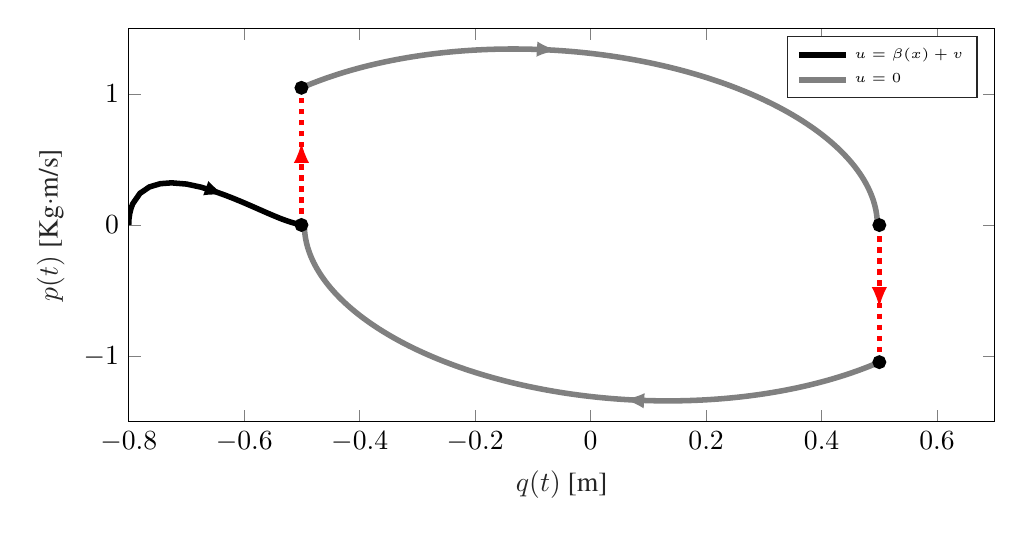
\begin{tikzpicture}

\begin{axis}[%
width=11cm,
height=5cm,
at={(0.858in,0.481in)},
scale only axis,
xmin=-0.8,
xmax=0.7,
xlabel style={font=\color{white!15!black}},
xlabel={$q(t)$ [m]},
ymin=-1.5,
ymax=1.5,
ylabel style={font=\color{white!15!black}},
ylabel={$p(t)$ [Kg$\cdot$m/s]},
axis background/.style={fill=white},
legend style={legend cell align=left, align=left, draw=white!15!black,font = \tiny}
]
\addplot [color=black, line width=2.0pt]
  table[row sep=crcr,]{%
-0.8	0\\
-0.79951111951868	0.0477490023739828\\
-0.79811008082095	0.0906814049403223\\
-0.795891468826249	0.129040235018852\\
-0.792944776187467	0.163070850946301\\
-0.780417561508645	0.242320881333726\\
-0.764029602799776	0.290882105288283\\
-0.745456884813622	0.315219542465047\\
-0.725973531204578	0.321858831515851\\
-0.69990596289271	0.312541815223776\\
-0.675182591346937	0.289301395597582\\
-0.652469688739267	0.258686651178381\\
-0.632345559216368	0.226662424348638\\
-0.617338757000783	0.200908238622252\\
-0.604082781999283	0.176797406770428\\
-0.592424562970695	0.154785703881097\\
-0.582229375736837	0.135162597784723\\
-0.571064115086853	0.113534463212202\\
-0.561683876754374	0.0954300404251315\\
-0.553799404485863	0.0804441932255335\\
-0.547142777898694	0.0681027880249668\\
-0.539436820468652	0.0541734856262629\\
-0.533271711347302	0.0435890995557684\\
-0.528402657479605	0.0359245809429889\\
-0.524404342745406	0.0299987837902473\\
-0.521127077977175	0.0251439597718699\\
-0.518368646475493	0.0212655963980143\\
-0.516056201969089	0.0182366052355743\\
-0.514075304343261	0.0157461737601636\\
-0.512245794028465	0.0134405137147038\\
-0.510679923857475	0.0115401758477533\\
-0.509344153381082	0.0100005938890359\\
-0.508187986884424	0.00869948182526219\\
-0.507171843510017	0.00754503027254173\\
-0.506289351619222	0.00656359218253137\\
-0.505524109227117	0.00573605303184072\\
-0.504855709483334	0.00502225535552957\\
-0.504267478547139	0.00439105697914647\\
-0.503752835833422	0.00384510307868501\\
-0.503302933885505	0.00337482506795194\\
-0.502908156125825	0.00296490777307626\\
-0.502560388348614	0.00260300126311856\\
-0.502254970332233	0.00228713018351576\\
-0.501986874345041	0.00201205792150197\\
-0.501751052269233	0.00177098338070987\\
-0.501543159535206	0.00155823940281332\\
-0.501360211144487	0.00137166878841184\\
-0.501199269031116	0.00120826818052683\\
-0.501057509775478	0.00106464244044825\\
-0.500997563859026	0.00100387390811712\\
-0.500941038274212	0.000946624036878844\\
-0.500887735750696	0.000892684078473881\\
-0.500837469394745	0.000841855322192339\\
}
[postaction={decorate, decoration={markings,
        mark=between positions 0.6 and 1 step 1 with {\arrow[black,line width=1.5pt]{latex};}
      }}];
\addlegendentry{$u = \beta(x)+v$}

\addplot [color=red, dotted, line width=2.0pt,forget plot]
  table[row sep=crcr]{%
-0.500837469394745	0.000841855322192339\\
-0.500837469394745	1.04598258627294\\
}
[postaction={decorate, decoration={markings,
        mark=between positions 0.6 and 1 step 1 with {\arrow[red,line width=1.5pt]{latex};}
      }}]
;

\addplot [color=gray, line width=2.0pt]
  table[row sep=crcr]{%
-0.500837469394745	1.04598258627294\\
-0.49979049724748	1.04796067094012\\
-0.498741550128628	1.04993252832074\\
-0.497690634268849	1.05189815167085\\
-0.496637755905533	1.05385753428104\\
-0.495582921282759	1.05581066947643\\
-0.494526136651266	1.05775755061672\\
-0.493467408268413	1.05969817109618\\
-0.492406742398151	1.0616325243437\\
-0.491344145310982	1.06356060382275\\
-0.490279623283929	1.06548240303147\\
-0.489213182600499	1.06739791550259\\
-0.488144829550648	1.06930713480355\\
-0.487074570430748	1.07121005453644\\
-0.486002411543552	1.07310666833803\\
-0.484928359198159	1.07499696987982\\
-0.483852419709978	1.07688095286799\\
-0.482774599400694	1.07875861104348\\
-0.481694904598237	1.08062993818197\\
-0.48061334163674	1.08249492809389\\
-0.47952991685651	1.08435357462444\\
-0.478444636603992	1.08620587165362\\
-0.477357507231732	1.08805181309623\\
-0.476268535098345	1.08989139290185\\
-0.475177726568479	1.09172460505492\\
-0.47408508801278	1.09355144357471\\
-0.472990625807857	1.09537190251532\\
-0.471894346336247	1.09718597596574\\
-0.470796255986381	1.09899365804982\\
-0.46969636115255	1.10079494292628\\
-0.468594668234867	1.10258982478878\\
-0.467491183639235	1.10437829786584\\
-0.46638591377731	1.10616035642095\\
-0.465278865066468	1.10793599475249\\
-0.464170043929769	1.1097052071938\\
-0.463059456795921	1.11146798811318\\
-0.461947110099249	1.11322433191389\\
-0.460833010279654	1.11497423303417\\
-0.459717163782583	1.11671768594723\\
-0.458599577058993	1.11845468516129\\
-0.457480256565313	1.12018522521956\\
-0.456359208763413	1.1219093007003\\
-0.455236440120568	1.12362690621676\\
-0.454111957109419	1.12533803641723\\
-0.452985766207944	1.12704268598506\\
-0.45185787389942	1.12874084963863\\
-0.450728286672388	1.13043252213141\\
-0.449597011020615	1.13211769825191\\
-0.448464053443067	1.13379637282374\\
-0.447329420443865	1.1354685407056\\
-0.446193118532255	1.13713419679126\\
-0.445055154222572	1.13879333600961\\
-0.443915534034204	1.14044595332466\\
-0.442774264491558	1.14209204373552\\
-0.441631352124023	1.14373160227644\\
-0.440486803465939	1.1453646240168\\
-0.439340625056556	1.14699110406111\\
-0.438192823440002	1.14861103754905\\
-0.437043405165252	1.15022441965543\\
-0.435892376786083	1.15183124559024\\
-0.434739744861047	1.15343151059861\\
-0.433585515953434	1.15502520996088\\
-0.432429696631236	1.15661233899255\\
-0.43127229346711	1.1581928930443\\
-0.430113313038346	1.159766867502\\
-0.42895276192683	1.16133425778674\\
-0.427790646719011	1.16289505935478\\
-0.426626974005863	1.1644492676976\\
-0.42546175038285	1.1659968783419\\
-0.424294982449892	1.16753788684959\\
-0.423126676811331	1.1690722888178\\
-0.421956840075892	1.17060007987888\\
-0.420785478856653	1.17212125570041\\
-0.419612599771004	1.17363581198522\\
-0.418438209440616	1.17514374447136\\
-0.417262314491403	1.17664504893213\\
-0.416084921553491	1.17813972117607\\
-0.414906037261176	1.17962775704696\\
-0.413725668252895	1.18110915242385\\
-0.412543821171189	1.18258390322104\\
-0.411360502662664	1.18405200538807\\
-0.410175719377961	1.18551345490976\\
-0.40898947797172	1.18696824780618\\
-0.407801785102539	1.18841638013266\\
-0.406612647432948	1.18985784797982\\
-0.405422071629365	1.19129264747351\\
-0.404230064362065	1.19272077477489\\
-0.403036632305147	1.19414222608038\\
-0.401841782136493	1.19555699762164\\
-0.400645520537737	1.19696508566565\\
-0.399447854194227	1.19836648651464\\
-0.398248789794994	1.19976119650613\\
-0.39704833403271	1.2011492120129\\
-0.39584649360366	1.20253052944301\\
-0.394643275207702	1.20390514523982\\
-0.393438685548233	1.20527305588193\\
-0.392232731332152	1.20663425788326\\
-0.391025419269831	1.20798874779298\\
-0.389816756075069	1.20933652219553\\
-0.388606748465069	1.21067757771066\\
-0.387395403160393	1.21201191099335\\
-0.38618272688493	1.21333951873391\\
-0.384968726365864	1.21466039765787\\
-0.383753408333633	1.21597454452606\\
-0.382536779521899	1.21728195613459\\
-0.381318846667507	1.21858262931481\\
-0.380099616510457	1.21987656093337\\
-0.378879095793861	1.22116374789216\\
-0.377657291263914	1.22244418712835\\
-0.376434209669855	1.22371787561436\\
-0.375209857763933	1.22498481035787\\
-0.373984242301372	1.22624498840183\\
-0.372757370040337	1.22749840682442\\
-0.371529247741893	1.22874506273909\\
-0.370299882169979	1.22998495329454\\
-0.369069280091363	1.23121807567468\\
-0.367837448275615	1.23244442709871\\
-0.366604393495067	1.23366400482102\\
-0.365370122524777	1.23487680613126\\
-0.3641346421425	1.23608282835429\\
-0.362897959128645	1.23728206885023\\
-0.361660080266244	1.23847452501437\\
-0.360421012340917	1.23966019427726\\
-0.359180762140835	1.24083907410462\\
-0.357939336456686	1.24201116199741\\
-0.35669674208164	1.24317645549177\\
-0.355452985811312	1.24433495215905\\
-0.354208074443729	1.24548664960577\\
-0.352962014779294	1.24663154547365\\
-0.35171481362075	1.24776963743958\\
-0.350466477773145	1.24890092321563\\
-0.3492170140438	1.25002540054903\\
-0.347966429242268	1.25114306722218\\
-0.346714730180303	1.25225392105261\\
-0.345461923671826	1.25335795989301\\
-0.344208016532885	1.25445518163123\\
-0.342953015581624	1.25554558419022\\
-0.341696927638246	1.25662916552807\\
-0.340439759524977	1.257705923638\\
-0.339181518066036	1.25877585654831\\
-0.337922210087593	1.25983896232243\\
-0.336661842417738	1.26089523905888\\
-0.335400421886444	1.26194468489127\\
-0.334137955325534	1.26298729798826\\
-0.332874449568645	1.26402307655363\\
-0.331609911451192	1.26505201882618\\
-0.330344347810333	1.26607412307978\\
-0.329077765484936	1.26708938762334\\
-0.327810171315542	1.26809781080083\\
-0.32654157214433	1.26909939099119\\
-0.325271974815084	1.27009412660844\\
-0.324001386173155	1.27108201610157\\
-0.322729813065428	1.27206305795457\\
-0.321457262340287	1.27303725068643\\
-0.320183740847578	1.2740045928511\\
-0.318909255438578	1.27496508303752\\
-0.317633812965955	1.27591871986957\\
-0.316357420283737	1.27686550200608\\
-0.315080084247277	1.27780542814081\\
-0.313801811713214	1.27873849700246\\
-0.312522609539442	1.27966470735463\\
-0.311242484585075	1.28058405799582\\
-0.30996144371041	1.28149654775943\\
-0.308679493776893	1.28240217551373\\
-0.307396641647085	1.28330094016187\\
-0.306112894184626	1.28419284064185\\
-0.3048282582542	1.2850778759265\\
-0.303542740721503	1.28595604502349\\
-0.302256348453202	1.28682734697532\\
-0.300969088316908	1.28769178085928\\
-0.299680967181136	1.28854934578746\\
-0.29839199191527	1.28940004090672\\
-0.297102169389532	1.29024386539871\\
-0.295811506474943	1.29108081847981\\
-0.294520010043293	1.29191089940114\\
-0.293227686967099	1.29273410744857\\
-0.29193454411958	1.29355044194267\\
-0.290640588374614	1.2943599022387\\
-0.289345826606706	1.29516248772661\\
-0.288050265690955	1.29595819783102\\
-0.286753912503019	1.29674703201122\\
-0.285456773919077	1.29752898976112\\
-0.284158856815798	1.29830407060927\\
-0.282860168070305	1.29907227411882\\
-0.281560714560141	1.29983359988754\\
-0.280260503163233	1.30058804754774\\
-0.27895954075786	1.30133561676635\\
-0.277657834222614	1.3020763072448\\
-0.276355390436372	1.30281011871908\\
-0.275052216278254	1.30353705095969\\
-0.273748318627596	1.30425710377165\\
-0.272443704363908	1.30497027699444\\
-0.271138380366845	1.30567657050203\\
-0.269832353516173	1.30637598420282\\
-0.268525630691728	1.30706851803967\\
-0.26721821877339	1.30775417198986\\
-0.265910124641041	1.30843294606504\\
-0.264601355174536	1.30910484031128\\
-0.263291917253668	1.30976985480901\\
-0.26198181775813	1.31042798967299\\
-0.260671063567484	1.31107924505234\\
-0.259359661561126	1.31172362113047\\
-0.258047618618251	1.31236111812511\\
-0.25673494161782	1.31299173628824\\
-0.255421637438523	1.31361547590612\\
-0.25410771295875	1.31423233729925\\
-0.252793175056549	1.31484232082235\\
-0.251478030609599	1.31544542686434\\
-0.250162286495173	1.31604165584831\\
-0.248845949590103	1.31663100823156\\
-0.247529026770747	1.31721348450548\\
-0.246211524912954	1.31778908519562\\
-0.244893450892031	1.31835781086164\\
-0.243574811582708	1.31891966209727\\
-0.242255613859104	1.31947463953032\\
-0.240935864594694	1.32002274382262\\
-0.239615570662274	1.32056397567007\\
-0.238294738933926	1.32109833580254\\
-0.236973376280986	1.32162582498389\\
-0.23565148957401	1.32214644401197\\
-0.234329085682737	1.32266019371853\\
-0.233006171476058	1.32316707496929\\
-0.231682753821984	1.32366708866384\\
-0.230358839587605	1.32416023573565\\
-0.229034435639065	1.32464651715206\\
-0.22770954884152	1.32512593391425\\
-0.22638418605911	1.32559848705719\\
-0.225058354154922	1.32606417764967\\
-0.22373205999096	1.32652300679424\\
-0.222405310428105	1.32697497562718\\
-0.221078112326087	1.32742008531851\\
-0.219750472543448	1.32785833707197\\
-0.21842239793751	1.32828973212496\\
-0.217093895364341	1.32871427174852\\
-0.215764971678721	1.32913195724735\\
-0.214435633734109	1.32954278995976\\
-0.213105888382607	1.32994677125762\\
-0.21177574247493	1.3303439025464\\
-0.210445202860371	1.33073418526508\\
-0.209114276386766	1.33111762088616\\
-0.207782969900463	1.33149421091564\\
-0.206451290246286	1.33186395689297\\
-0.205119244267504	1.33222686039108\\
-0.203786838805796	1.33258292301627\\
-0.202454080701216	1.33293214640825\\
-0.201120976792166	1.33327453224012\\
-0.199787533915354	1.3336100822183\\
-0.198453758905768	1.33393879808252\\
-0.197119658596637	1.33426068160583\\
-0.195785239819401	1.33457573459453\\
-0.19445050940368	1.33488395888815\\
-0.193115474177233	1.33518535635946\\
-0.191780140965933	1.33547992891441\\
-0.19044451659373	1.3357676784921\\
-0.189108607882618	1.33604860706479\\
-0.187772421652601	1.33632271663783\\
-0.186435964721663	1.33659000924967\\
-0.185099243905732	1.3368504869718\\
-0.183762266018648	1.33710415190877\\
-0.182425037872131	1.33735100619809\\
-0.181087566275745	1.33759105201029\\
-0.179749858036868	1.33782429154881\\
-0.17841191996066	1.33805072705005\\
-0.177073758850025	1.33827036078327\\
-0.175735381505582	1.33848319505062\\
-0.174396794725634	1.33868923218708\\
-0.17305800530613	1.33888847456042\\
-0.171719020040634	1.33908092457123\\
-0.170379845720297	1.33926658465282\\
-0.169040489133817	1.33944545727125\\
-0.16770095706741	1.33961754492525\\
-0.166361256304778	1.33978285014624\\
-0.165021393627074	1.33994137549827\\
-0.163681375812872	1.340093123578\\
-0.162341209638133	1.34023809701466\\
-0.16100090187617	1.34037629847005\\
-0.159660459297622	1.34050773063847\\
-0.158319888670414	1.34063239624673\\
-0.156979196759729	1.34075029805409\\
-0.155638390327976	1.34086143885224\\
-0.154297476134753	1.34096582146528\\
-0.152956460936822	1.34106344874967\\
-0.151615351488068	1.34115432359422\\
-0.150274154539473	1.34123844892005\\
-0.148932876839083	1.34131582768054\\
-0.147591525131972	1.34138646286134\\
-0.146250106160215	1.34145035748032\\
-0.144908626662849	1.34150751458751\\
-0.14356709337585	1.34155793726511\\
-0.142225513032091	1.34160162862746\\
-0.140883892361318	1.34163859182096\\
-0.139542238090113	1.34166883002408\\
-0.138200556941864	1.34169234644733\\
-0.136858855636731	1.34170914433321\\
-0.135517140891619	1.34171922695618\\
-0.134175419420138	1.34172259762262\\
-0.13283369793258	1.34171925967084\\
-0.13149198313588	1.34170921647097\\
-0.130150281733587	1.34169247142502\\
-0.128808600425834	1.34166902796678\\
-0.127466945909303	1.34163888956179\\
-0.126125324877194	1.34160205970736\\
-0.124783744019195	1.34155854193247\\
-0.123442210021449	1.34150833979778\\
-0.122100729566522	1.34145145689558\\
-0.120759309333373	1.34138789684977\\
-0.119417955997319	1.34131766331581\\
-0.118076676230009	1.34124075998068\\
-0.116735476699386	1.34115719056287\\
-0.115394364069661	1.34106695881233\\
-0.114053345001279	1.34097006851045\\
-0.112712426150887	1.34086652346999\\
-0.111371614171304	1.34075632753509\\
-0.11003091571149	1.3406394845812\\
-0.108690337416512	1.34051599851508\\
-0.107349885927518	1.34038587327473\\
-0.106009567881698	1.34024911282936\\
-0.104669389912261	1.34010572117938\\
-0.103329358648398	1.33995570235634\\
-0.101989480715252	1.33979906042291\\
-0.100649762733891	1.33963579947282\\
-0.0993102113212709	1.33946592363087\\
-0.0979708330902083	1.33928943705283\\
-0.0966316346493487	1.33910634392546\\
-0.095292622603135	1.33891664846645\\
-0.0939538035517772	1.33872035492437\\
-0.0926151840912212	1.33851746757866\\
-0.091276770813118	1.33830799073959\\
-0.089938570304793	1.33809192874819\\
-0.0886005891492154	1.33786928597627\\
-0.0872628339249669	1.33764006682632\\
-0.0859253112062114	1.33740427573153\\
-0.0845880275626645	1.33716191715569\\
-0.0832509895595626	1.33691299559323\\
-0.0819142037576322	1.33665751556911\\
-0.0805776767130602	1.33639548163882\\
-0.0792414149774617	1.33612689838834\\
-0.0779054250978517	1.33585177043408\\
-0.0765697136166129	1.33557010242289\\
-0.075234287071466	1.33528189903195\\
-0.07389915199544	1.3349871649688\\
-0.0725643149168403	1.33468590497125\\
-0.07122978235922	1.33437812380739\\
-0.0698955608413485	1.3340638262755\\
-0.0685616568771824	1.33374301720404\\
-0.0672280769758344	1.33341570145162\\
-0.0658948276415436	1.33308188390693\\
-0.0645619153736455	1.33274156948872\\
-0.0632293466665414	1.33239476314576\\
-0.0618971280096696	1.33204146985681\\
-0.060565265887474	1.33168169463055\\
-0.0592337667793751	1.33131544250557\\
-0.05790263715974	1.33094271855029\\
-0.0565718834978522	1.330563527863\\
-0.0552415122578822	1.33017787557171\\
-0.0539115298988578	1.32978576683421\\
-0.0525819428746338	1.32938720683797\\
-0.0512527576338628	1.3289822008001\\
-0.0499239806199655	1.32857075396735\\
-0.0485956182711013	1.32815287161603\\
-0.047267677020138	1.32772855905198\\
-0.0459401632946234	1.32729782161054\\
-0.0446130835167548	1.32686066465648\\
-0.0432864441033503	1.32641709358401\\
-0.0419602514658187	1.32596711381667\\
-0.0406345120101312	1.32551073080736\\
-0.039309232136791	1.32504795003823\\
-0.0379844182408046	1.32457877702069\\
-0.0366600767116525	1.32410321729535\\
-0.0353362139332602	1.32362127643196\\
-0.0340128362839687	1.32313296002939\\
-0.0326899501365054	1.32263827371559\\
-0.0313675618579557	1.32213722314753\\
-0.0300456778097334	1.32162981401117\\
-0.0287243043475516	1.3211160520214\\
-0.0274034478213942	1.32059594292203\\
-0.0260831145754869	1.32006949248572\\
-0.0247633109482682	1.31953670651392\\
-0.0234440432723611	1.31899759083689\\
-0.0221253178745435	1.31845215131358\\
-0.0208071410757205	1.31790039383165\\
-0.0194895191908947	1.31734232430737\\
-0.0181724585291384	1.31677794868564\\
-0.016855965393565	1.31620727293987\\
-0.0155400460812999	1.31563030307202\\
-0.0142247068834518	1.31504704511249\\
-0.0129099540850861	1.31445750512009\\
-0.0115957939651936	1.31386168918201\\
-0.0102822327966659	1.31325960341378\\
-0.00896927684626214	1.31265125395921\\
-0.00765693237458575	1.31203664699033\\
-0.0063452056360531	1.3114157887074\\
-0.00503410287886636	1.3107886853388\\
-0.00372363034498555	1.31015534314103\\
-0.00241379427009969	1.30951576839864\\
-0.0011046008835993	1.30886996742419\\
0.000203943591451302	1.30821794655822\\
0.0015118329383424	1.30755971216918\\
0.00281906094674719	1.30689527065342\\
0.00412562141274814	1.30622462843508\\
0.00543150813886684	1.30554779196613\\
0.00673671493408997	1.30486476772624\\
0.00804123561389757	1.3041755622228\\
0.00934506400029216	1.30348018199082\\
0.0106481939218239	1.30277863359294\\
0.0119506192136194	1.30207092361932\\
0.0132523337174095	1.30135705868766\\
0.0145533312815565	1.30063704544308\\
0.0158536057610819	1.29991089055815\\
0.0171531510176924	1.29917860073278\\
0.0184519609198095	1.2984401826942\\
0.0197500293425944	1.29769564319693\\
0.0210473501679772	1.29694498902268\\
0.0223439172846833	1.29618822698038\\
0.0236397245882604	1.29542536390605\\
0.0249347659811057	1.29465640666281\\
0.0262290353724928	1.29388136214079\\
0.0275225266785995	1.29310023725714\\
0.0288152338225342	1.29231303895592\\
0.0301071507343621	1.29151977420809\\
0.0313982713511336	1.29072045001144\\
0.0326885896169101	1.28991507339056\\
0.0339780994827902	1.28910365139678\\
0.0352667949069385	1.28828619110812\\
0.0365546698546095	1.28746269962926\\
0.0378417182981771	1.28663318409146\\
0.0391279342171583	1.28579765165254\\
0.0404133115982428	1.28495610949682\\
0.0416978444353165	1.28410856483506\\
0.0429815267294897	1.28325502490442\\
0.0442643524891232	1.28239549696842\\
0.0455463157298544	1.28152998831687\\
0.0468274104746235	1.28065850626586\\
0.0481076307537001	1.27978105815765\\
0.049386970604709	1.27889765136066\\
0.0506654240726563	1.27800829326943\\
0.0519429852099562	1.27711299130453\\
0.0532196480764561	1.27621175291255\\
0.0544954067394627	1.27530458556602\\
0.055770255273769	1.27439149676338\\
0.0570441877616786	1.27347249402892\\
0.0583171982930327	1.27254758491272\\
0.0595892809652352	1.27161677699064\\
0.0608604298832792	1.27068007786421\\
0.0621306391597711	1.26973749516061\\
0.0633999029149586	1.26878903653264\\
0.064668215276754	1.26783470965862\\
0.0659355703807614	1.2668745222424\\
0.0672019623703011	1.26590848201323\\
0.0684673853964348	1.2649365967258\\
0.0697318336179926	1.2639588741601\\
0.0709953012015971	1.26297532212143\\
0.0722577823216878	1.26198594844034\\
0.0735192711605486	1.26099076097254\\
0.0747797619083308	1.2599897675989\\
0.0760392487630796	1.25898297622535\\
0.0772977259307582	1.25797039478287\\
0.078555187625274	1.2569520312274\\
0.0798116280685019	1.25592789353983\\
0.0810670414903111	1.2548979897259\\
0.0823214221285883	1.25386232781619\\
0.0835747642292631	1.25282091586604\\
0.0848270620463332	1.2517737619555\\
0.0860783098418888	1.2507208741893\\
0.087328501886136	1.24966226069676\\
0.0885776324574246	1.24859792963179\\
0.0898256958422682	1.24752788917277\\
0.0910726863353727	1.24645214752255\\
0.0923185982396584	1.24537071290837\\
0.093563425866285	1.24428359358182\\
0.0948071635346761	1.24319079781879\\
0.0960498055725434	1.2420923339194\\
0.0972913463159107	1.24098821020794\\
0.0985317801091379	1.23987843503286\\
0.0997711013049459	1.23876301676666\\
0.10100930426444	1.23764196380589\\
0.102246383357133	1.23651528457104\\
0.103482332960971	1.23538298750653\\
0.104717147462358	1.23424508108065\\
0.105950821256176	1.23310157378548\\
0.107183348745811	1.23195247413687\\
0.108414724343178	1.23079779067435\\
0.109644942468743	1.22963753196109\\
0.110873997551545	1.22847170658388\\
0.112101884029226	1.22730032315301\\
0.113328596348044	1.22612339030227\\
0.114554128962909	1.22494091668886\\
0.115778476337395	1.22375291099337\\
0.11700163294377	1.22255938191967\\
0.118223593263017	1.22136033819493\\
0.119444351784859	1.22015578856949\\
0.12066390300778	1.21894574181687\\
0.121882241439049	1.21773020673364\\
0.123099361594743	1.21650919213945\\
0.124315257999771	1.21528270687692\\
0.125529925187896	1.21405075981158\\
0.126743357701756	1.21281335983184\\
0.127955550092892	1.21157051584893\\
0.129166496921764	1.21032223679684\\
0.13037619275778	1.20906853163226\\
0.131584632179317	1.20780940933451\\
0.132791809773739	1.20654487890553\\
0.133997720137426	1.20527494936977\\
0.135202357875792	1.20399962977417\\
0.13640571760331	1.20271892918809\\
0.137607793943535	1.20143285670325\\
0.138808581529122	1.20014142143367\\
0.140008075001852	1.19884463251565\\
0.141206269012656	1.19754249910766\\
0.142403158221631	1.19623503039031\\
0.143598737298068	1.19492223556629\\
0.14479300092047	1.19360412386033\\
0.145985943776576	1.19228070451911\\
0.147177560563385	1.19095198681122\\
0.148367845987173	1.18961798002712\\
0.149556794763518	1.18827869347903\\
0.150744401617321	1.18693413650095\\
0.151930661282828	1.18558431844852\\
0.153115568503652	1.18422924869903\\
0.154299118032793	1.18286893665132\\
0.155481304632662	1.18150339172574\\
0.156662123075099	1.1801326233641\\
0.157841568141399	1.17875664102959\\
0.159019634622329	1.17737545420672\\
0.160196317318151	1.1759890724013\\
0.161371611038646	1.17459750514034\\
0.162545510603129	1.17320076197201\\
0.163718010840477	1.1717988524656\\
0.164889106589144	1.17039178621142\\
0.166058792697187	1.16897957282076\\
0.167227064022284	1.16756222192585\\
0.168393915431755	1.16613974317978\\
0.169559341802584	1.16471214625644\\
0.17072333802144	1.1632794408505\\
0.171885898984696	1.16184163667727\\
0.17304701959845	1.16039874347273\\
0.174206694778549	1.15895077099341\\
0.175364919450605	1.15749772901638\\
0.176521688550015	1.15603962733913\\
0.177676997021988	1.15457647577957\\
0.17883083982156	1.15310828417592\\
0.179983211913612	1.15163506238672\\
0.181134108272897	1.15015682029067\\
0.182283523884057	1.14867356778668\\
0.18343145374164	1.14718531479372\\
0.184577892850127	1.14569207125081\\
0.185722836223945	1.14419384711696\\
0.18686627888749	1.14269065237107\\
0.188008215875149	1.14118249701194\\
0.189148642231316	1.13966939105813\\
0.190287553010413	1.13815134454796\\
0.191424943276912	1.13662836753942\\
0.192560808105351	1.13510047011012\\
0.193695142580358	1.13356766235723\\
0.194827941796663	1.13202995439742\\
0.195959200859129	1.1304873563668\\
0.197088914882758	1.12893987842085\\
0.198217078992723	1.12738753073437\\
0.199343688324378	1.12583032350141\\
0.200468738023281	1.12426826693523\\
0.201592223245215	1.12270137126822\\
0.202714139156201	1.12112964675184\\
0.203834480932525	1.11955310365656\\
0.204953243760751	1.11797175227182\\
0.206070422837742	1.11638560290593\\
0.207186013370678	1.11479466588605\\
0.208300010577077	1.1131989515581\\
0.209412409684812	1.11159847028671\\
0.21052320593213	1.10999323245516\\
0.21163239456767	1.10838324846532\\
0.212739970850481	1.10676852873756\\
0.213845930050045	1.10514908371076\\
0.214950267446289	1.10352492384217\\
0.216052978329608	1.10189605960737\\
0.217154058000879	1.10026250150026\\
0.218253501771488	1.09862426003293\\
0.219351304963335	1.09698134573562\\
0.220447462908865	1.09533376915668\\
0.221541970951076	1.0936815408625\\
0.222634824443546	1.09202467143741\\
0.223726018750442	1.09036317148369\\
0.224815549246543	1.08869705162143\\
0.225903411317261	1.08702632248853\\
0.226989600358649	1.08535099474059\\
0.228074111777428	1.08367107905089\\
0.229156940991	1.08198658611031\\
0.230238083427467	1.08029752662726\\
0.231317534525649	1.07860391132761\\
0.232395289735098	1.07690575095467\\
0.23347134451612	1.07520305626907\\
0.234545694339791	1.07349583804876\\
0.235618334687971	1.07178410708888\\
0.236689261053326	1.07006787420175\\
0.237758468939342	1.06834715021679\\
0.238825953860342	1.06662194598046\\
0.239891711341507	1.06489227235617\\
0.240955736918885	1.06315814022428\\
0.242018026139418	1.06141956048196\\
0.24307857456095	1.05967654404318\\
0.244137377752249	1.05792910183865\\
0.245194431293021	1.05617724481571\\
0.246249730773929	1.05442098393831\\
0.247303271796606	1.05266033018694\\
0.248355049973677	1.05089529455855\\
0.249405060928769	1.04912588806649\\
0.250453300296532	1.04735212174048\\
0.251499763722653	1.04557400662649\\
0.252544446863876	1.04379155378672\\
0.253587345388011	1.04200477429953\\
0.254628454973957	1.04021367925937\\
0.255667771311715	1.03841827977669\\
0.256705290102405	1.03661858697794\\
0.25774100705828	1.03481461200544\\
0.258774917902744	1.03300636601737\\
0.259807018370367	1.03119386018767\\
0.260837304206902	1.02937710570598\\
0.261865771169297	1.02755611377759\\
0.262892415025715	1.02573089562339\\
0.263917231555547	1.02390146247975\\
0.264940216549428	1.02206782559854\\
0.265961365809254	1.02022999624696\\
0.266980675148193	1.0183879857076\\
0.267998140390705	1.01654180527825\\
0.269013757372557	1.01469146627194\\
0.270027521940833	1.01283698001682\\
0.271039429953955	1.01097835785609\\
0.272049477281696	1.00911561114799\\
0.273057659805193	1.00724875126567\\
0.274063973416965	1.00537778959716\\
0.275068414020926	1.00350273754531\\
0.2760709775324	1.00162360652772\\
0.277071659878137	0.999740407976657\\
0.278070456996324	0.997853153339021\\
0.279067364836606	0.995961854076256\\
0.280062379360093	0.994066521664299\\
0.281055496539382	0.992167167593508\\
0.282046712358562	0.990263803368605\\
0.28303602281324	0.988356440508602\\
0.284023423910545	0.986445090546744\\
0.285008911669149	0.98452976503044\\
0.285992482119275	0.982610475521202\\
0.286974131302718	0.980687233594575\\
0.287953855272855	0.978760050840075\\
0.288931650094657	0.976828938861125\\
0.289907511844708	0.974893909274988\\
0.290881436611215	0.972954973712705\\
0.291853420494023	0.971012143819026\\
0.292823459604628	0.969065431252346\\
0.293791550066194	0.967114847684643\\
0.294757688013559	0.96516040480141\\
0.295721869593257	0.963202114301589\\
0.296684090963527	0.961239987897509\\
0.297644348294326	0.959274037314819\\
0.298602637767343	0.957304274292422\\
0.299558955576015	0.955330710582409\\
0.300513297925534	0.953353357949998\\
0.301465661032867	0.951372228173465\\
0.302416041126763	0.949387333044079\\
0.303364434447772	0.947398684366034\\
0.304310837248251	0.945406293956392\\
0.305255245792384	0.943410173645006\\
0.306197656356188	0.941410335274467\\
0.307138065227531	0.939406790700026\\
0.308076468706143	0.937399551789536\\
0.309012863103625	0.935388630423387\\
0.309947244743469	0.933374038494434\\
0.310879609961062	0.931355787907938\\
0.311809955103704	0.929333890581498\\
0.312738276530621	0.927308358444982\\
0.313664570612971	0.925279203440467\\
0.314588833733864	0.923246437522167\\
0.315511062288367	0.921210072656375\\
0.31643125268352	0.919170120821388\\
0.31734940133835	0.917126594007449\\
0.318265504683876	0.915079504216676\\
0.319179559163128	0.913028863462999\\
0.320091561231156	0.910974683772091\\
0.321001507355039	0.908916977181306\\
0.321909394013901	0.906855755739611\\
0.322815217698921	0.904791031507517\\
0.323718974913344	0.902722816557018\\
0.32462066217249	0.900651122971525\\
0.325520276003773	0.898575962845792\\
0.326417812946704	0.896497348285861\\
0.327313269552906	0.894415291408988\\
0.328206642386125	0.892329804343577\\
0.329097928022243	0.89024089922912\\
0.329987123049284	0.888148588216125\\
0.330874224067429	0.88605288346605\\
0.331759227689028	0.88395379715124\\
0.332642130538605	0.881851341454859\\
0.333522929252875	0.879745528570823\\
0.334401620480752	0.877636370703735\\
0.335278200883359	0.875523880068816\\
0.336152667134042	0.873408068891843\\
0.337025015918374	0.87128894940908\\
0.337895243934174	0.869166533867209\\
0.338763347891508	0.867040834523269\\
0.339629324512709	0.864911863644587\\
0.340493170532378	0.86277963350871\\
0.341354882697402	0.860644156403342\\
0.34221445776696	0.858505444626272\\
0.343071892512534	0.856363510485313\\
0.343927183717916	0.854218366298236\\
0.344780328179224	0.852070024392697\\
0.345631322704907	0.849918497106175\\
0.346480164115758	0.847763796785906\\
0.34732684924492	0.845605935788814\\
0.348171374937899	0.843444926481447\\
0.349013738052571	0.841280781239908\\
0.349853935459196	0.839113512449787\\
0.35069196404042	0.836943132506101\\
0.351527820691292	0.834769653813219\\
0.352361502319268	0.832593088784804\\
0.353193005844223	0.830413449843734\\
0.354022328198461	0.82823074942205\\
0.354849466326721	0.826044999960877\\
0.355674417186187	0.823856213910368\\
0.356497177746498	0.821664403729626\\
0.357317744989758	0.819469581886647\\
0.358136115910543	0.817271760858244\\
0.358952287515908	0.815070953129992\\
0.359766256825401	0.81286717119615\\
0.360578020871066	0.8106604275596\\
0.361387576697456	0.808450734731778\\
0.362194921361639	0.80623810523261\\
0.363000051933207	0.804022551590441\\
0.363802965494285	0.801804086341974\\
0.364603659139537	0.799582722032194\\
0.36540212997618	0.797358471214312\\
0.366198375123984	0.795131346449691\\
0.366992391715286	0.792901360307781\\
0.367784176894999	0.79066852536605\\
0.368573727820614	0.788432854209924\\
0.369361041662212	0.786194359432711\\
0.370146115602472	0.783953053635543\\
0.370928946836679	0.781708949427298\\
0.371709532572729	0.779462059424545\\
0.372487870031138	0.777212396251471\\
0.373263956445052	0.774959972539814\\
0.374037789060251	0.772704800928795\\
0.374809365135159	0.770446894065059\\
0.375578681940848	0.768186264602595\\
0.376345736761051	0.765922925202681\\
0.377110526892164	0.763656888533809\\
0.377873049643254	0.761388167271625\\
0.37863330233607	0.759116774098854\\
0.379391282305045	0.756842721705243\\
0.380146986897306	0.754566022787481\\
0.38090041347268	0.752286690049148\\
0.381651559403701	0.750004736200632\\
0.382400422075617	0.747720173959075\\
0.383146998886396	0.745433016048298\\
0.383891287246733	0.743143275198737\\
0.384633284580059	0.740850964147378\\
0.385372988322542	0.738556095637684\\
0.386110395923098	0.736258682419536\\
0.386845504843397	0.733958737249161\\
0.387578312557867	0.731656272889062\\
0.388308816553701	0.729351302107961\\
0.389037014330867	0.727043837680723\\
0.389762903402108	0.724733892388294\\
0.390486481292951	0.722421479017629\\
0.391207745541714	0.720106610361632\\
0.391926693699512	0.717789299219083\\
0.392643323330258	0.715469558394577\\
0.393357632010677	0.713147400698449\\
0.394069617330303	0.710822838946716\\
0.394779276891492	0.708495885961004\\
0.395486608309423	0.706166554568481\\
0.396191609212105	0.703834857601796\\
0.396894277240381	0.701500807899006\\
0.397594610047939	0.699164418303511\\
0.398292605301307	0.696825701663988\\
0.398988260679869	0.694484670834324\\
0.399681573875865	0.692141338673548\\
0.400372542594394	0.689795718045766\\
0.401061164553424	0.687447821820091\\
0.401747437483793	0.685097662870581\\
0.402431359129217	0.682745254076166\\
0.403112927246292	0.680390608320587\\
0.4037921396045	0.678033738492327\\
0.404468993986216	0.675674657484542\\
0.405143488186709	0.673313378194996\\
0.405815620014147	0.670949913525999\\
0.406485387289603	0.668584276384328\\
0.407152787847061	0.666216479681176\\
0.407817819533417	0.66384653633207\\
0.408480480208483	0.661474459256817\\
0.409140767744997	0.659100261379427\\
0.409798680028617	0.656723955628056\\
0.410454214957939	0.654345554934928\\
0.411107370444486	0.651965072236281\\
0.411758144412723	0.649582520472289\\
0.412406534800056	0.647197912587004\\
0.413052539556839	0.644811261528282\\
0.413696156646372	0.642422580247723\\
0.414337384044912	0.640031881700601\\
0.414976219741671	0.637639178845795\\
0.415612661738822	0.635244484645729\\
0.416246708051503	0.632847812066299\\
0.416878356707818	0.63044917407681\\
0.417507605748843	0.62804858364991\\
0.41813445322863	0.625646053761519\\
0.418758897214206	0.623241597390768\\
0.419380935785579	0.620835227519927\\
0.420000567035741	0.618426957134346\\
0.420617789070672	0.616016799222383\\
0.42123260000934	0.613604766775334\\
0.421844997983709	0.611190872787379\\
0.422454981138734	0.6087751302555\\
0.423062547632372	0.606357552179429\\
0.423667695635579	0.603938151561572\\
0.424270423332316	0.601516941406946\\
0.424870728919549	0.599093934723114\\
0.425468610607256	0.596669144520114\\
0.426064066618421	0.594242583810401\\
0.426657095189046	0.59181426560877\\
0.427247694568147	0.5893842029323\\
0.427835863017759	0.586952408800282\\
0.428421598812936	0.584518896234153\\
0.429004900241757	0.582083678257431\\
0.429585765605322	0.579646767895652\\
0.430164193217762	0.577208178176295\\
0.430740181406232	0.574767922128726\\
0.43131372851092	0.572326012784127\\
0.431884832885046	0.569882463175429\\
0.432453492894861	0.567437286337248\\
0.433019706919656	0.564990495305817\\
0.433583473351754	0.562542103118926\\
0.434144790596522	0.560092122815847\\
0.434703657072361	0.557640567437273\\
0.435260071210718	0.555187450025255\\
0.435814031456081	0.552732783623128\\
0.436365536265983	0.550276581275454\\
0.436914584110999	0.547818856027952\\
0.437461173474754	0.545359620927429\\
0.438005302853919	0.54289888902172\\
0.438546970758212	0.540436673359619\\
0.439086175710403	0.537972986990816\\
0.439622916246309	0.535507842965828\\
0.440157190914799	0.533041254335934\\
0.440688998277796	0.530573234153113\\
0.441218336910272	0.528103795469972\\
0.441745205400254	0.525632951339686\\
0.44226960234882	0.523160714815931\\
0.442791526370106	0.520687098952818\\
0.443310976091298	0.518212116804826\\
0.443827950152639	0.515735781426739\\
0.444342447207426	0.513258105873581\\
0.444854465922012	0.510779103200546\\
0.445364004975806	0.508298786462939\\
0.445871063061268	0.505817168716108\\
0.44637563888392	0.503334263015375\\
0.446877731162333	0.500850082415978\\
0.447377338628137	0.498364639972998\\
0.447874460026016	0.495877948741302\\
0.448369094113709	0.49339002177547\\
0.448861239662007	0.490900872129736\\
0.449350895454759	0.488410512857918\\
0.449838060288865	0.485918957013357\\
0.450322732974279	0.483426217648851\\
0.450804912334007	0.480932307816587\\
0.451284597204107	0.47843724056808\\
0.451761786433688	0.475941028954107\\
0.45223647888491	0.473443686024639\\
0.452708673432982	0.470945224828784\\
0.453178368966162	0.46844565841471\\
0.453645564385755	0.465944999829592\\
0.454110258606113	0.463443262119543\\
0.454572450554634	0.460940458329546\\
0.45503213917176	0.458436601503392\\
0.455489323410976	0.455931704683621\\
0.455944002238809	0.453425780911444\\
0.456396174634828	0.450918843226694\\
0.456845839591638	0.448410904667748\\
0.457292996114884	0.445901978271472\\
0.457737643223247	0.443392077073154\\
0.458179779948441	0.440881214106434\\
0.458619405335215	0.43836940240325\\
0.459056518441345	0.435856654993765\\
0.459491118337643	0.433342984906306\\
0.459923204107941	0.430828405167302\\
0.460352774849102	0.428312928801214\\
0.460779829671009	0.425796568830476\\
0.461204367696568	0.423279338275432\\
0.461626388061704	0.420761250154264\\
0.46204588991536	0.418242317482938\\
0.462462872419491	0.415722553275134\\
0.462877334749068	0.413201970542181\\
0.46328927609207	0.410680582292999\\
0.463698695649484	0.408158401534029\\
0.464105592635303	0.405635441269174\\
0.464509966276521	0.403111714499733\\
0.464911815813134	0.400587234224335\\
0.465311140498133	0.398062013438882\\
0.465707939597506	0.395536065136478\\
0.46610221239023	0.39300940230737\\
0.466493958168274	0.390482037938883\\
0.46688317623659	0.387953985015358\\
0.467269865913114	0.385425256518085\\
0.467654026528761	0.382895865425243\\
0.468035657427424	0.380365824711838\\
0.468414757965968	0.377835147349633\\
0.46879132751423	0.375303846307093\\
0.469165365455011	0.372771934549316\\
0.469536871184078	0.370239425037973\\
0.469905844110155	0.367706330731242\\
0.470272283654926	0.365172664583749\\
0.470636189253026	0.362638439546502\\
0.470997560352039	0.360103668566829\\
0.471356396412494	0.357568364588313\\
0.471712696907862	0.355032540550735\\
0.472066461324554	0.352496209390003\\
0.472417689161912	0.349959384038097\\
0.472766379932209	0.347422077423002\\
0.473112533160645	0.344884302468646\\
0.47345614838534	0.342346072094837\\
0.473797225157333	0.339807399217203\\
0.474135763040577	0.337268296747127\\
0.474471761611933	0.334728777591685\\
0.474805220461166	0.332188854653585\\
0.475136139190945	0.329648540831101\\
0.475464517416832	0.327107849018016\\
0.475790354767281	0.324566792103558\\
0.476113650883633	0.322025382972333\\
0.476434405420113	0.319483634504272\\
0.476752618043821	0.31694155957456\\
0.477068288434732	0.31439917105358\\
0.477381416285687	0.311856481806848\\
0.47769200130239	0.309313504694952\\
0.478000043203407	0.306770252573491\\
0.478305541720151	0.304226738293012\\
0.478608496596888	0.301682974698949\\
0.478908907590725	0.299138974631561\\
0.479206774471605	0.296594750925872\\
0.479502097022307	0.294050316411605\\
0.479794875038434	0.291505683913127\\
0.480085108328412	0.28896086624938\\
0.480372796713482	0.286415876233827\\
0.480657940027698	0.283870726674387\\
0.480940538117917	0.281325430373373\\
0.481220590843797	0.278780000127433\\
0.481498098077788	0.276234448727487\\
0.481773059705129	0.273688788958668\\
0.482045475623841	0.271143033600257\\
0.482315345744724	0.268597195425629\\
0.482582669991343	0.266051287202184\\
0.482847448300032	0.263505321691292\\
0.483109680619882	0.26095931164823\\
0.483369366912735	0.258413269822121\\
0.48362650715318	0.255867208955875\\
0.483881101328545	0.253321141786126\\
0.484133149438894	0.250775081043175\\
0.484382651497015	0.248229039450923\\
0.484629607528419	0.245683029726821\\
0.484874017571329	0.243137064581798\\
0.485115881676677	0.240591156720208\\
0.485355199908096	0.238045318839771\\
0.485591972341914	0.235499563631506\\
0.485826199067145	0.232953903779676\\
0.486057880185485	0.230408351961727\\
0.486287015811303	0.22786292084823\\
0.486513606071637	0.225317623102815\\
0.486737651106184	0.222772471382117\\
0.486959151067293	0.220227478335715\\
0.487178106119961	0.21768265660607\\
0.487394516441822	0.215138018828469\\
0.487608382223145	0.212593577630962\\
0.487819703666818	0.210049345634303\\
0.488028480988351	0.207505335451894\\
0.488234714415862	0.204961559689722\\
0.48843840419007	0.202418030946299\\
0.488639550564291	0.199874761812607\\
0.488838153804427	0.197331764872035\\
0.489034214188958	0.194789052700323\\
0.48922773200894	0.192246637865497\\
0.489418707567988	0.189704532927821\\
0.489607141182279	0.187162750439724\\
0.489793033180533	0.184621302945753\\
0.489976383904014	0.182080202982509\\
0.490157193706518	0.179539463078589\\
0.490335462954364	0.176999095754528\\
0.490511192026391	0.174459113522737\\
0.490684381313942	0.171919528887449\\
0.490855031220863	0.169380354344663\\
0.491023142163492	0.166841602382074\\
0.491188714570647	0.164303285479029\\
0.491351748883626	0.161765416106458\\
0.491512245556191	0.159228006726822\\
0.491670205054563	0.156691069794052\\
0.49182562785741	0.154154617753493\\
0.491978514455846	0.151618663041845\\
0.492128865353413	0.149083218087102\\
0.492276681066079	0.146548295308502\\
0.492421962122226	0.144013907116464\\
0.492564709062641	0.141480065912526\\
0.492704922440511	0.138946784089299\\
0.492842602821408	0.1364140740304\\
0.492977750783285	0.133881948110398\\
0.493110366916464	0.131350418694755\\
0.493240451823628	0.128819498139772\\
0.493368006119813	0.126289198792529\\
0.493493030432395	0.12375953299083\\
0.493615525401086	0.121230513063143\\
0.493735491677919	0.118702151328545\\
0.493852929927244	0.116174460096664\\
0.493967840825714	0.113647451667627\\
0.494080225062277	0.111121138331994\\
0.494190083338169	0.108595532370711\\
0.494297416366901	0.106070646055047\\
0.494402224874248	0.103546491646539\\
0.494504509598247	0.101023081396938\\
0.494604271289176	0.0985004275481485\\
0.494701510709554	0.095978542332177\\
0.494796228634126	0.0934574379710722\\
0.494888425849852	0.0909371266768686\\
0.494978103155902	0.0884176206515356\\
0.495065261363642	0.0858989320869127\\
0.495149901296623	0.0833810731646634\\
0.495232023790576	0.0808640560562117\\
0.495311629693394	0.0783478929226915\\
0.49538871986513	0.0758325959148862\\
0.49546329517798	0.0733181771731799\\
0.495535356516275	0.0708046488274919\\
0.495604904776473	0.0682920229972342\\
0.495671940867145	0.0657803117912433\\
0.495736465708963	0.0632695273077332\\
0.495798480234697	0.0607596816342378\\
0.495857985389194	0.0582507868475567\\
0.495914982129376	0.0557428550136974\\
0.495969471424225	0.0532358981878242\\
0.49602145425477	0.0507299284141997\\
0.496070931614082	0.0482249577261345\\
0.496117904507258	0.0457209981459258\\
0.496162373951413	0.0432180616848116\\
0.496204340975667	0.0407161603429072\\
0.496243806621135	0.0382153061091593\\
0.496280771940915	0.0357155109612825\\
0.496315238000075	0.033216786865715\\
0.496347205875648	0.0307191457775546\\
0.496376676656614	0.0282225996405136\\
0.496403651443891	0.0257271603868576\\
0.496428131350323	0.023232839937356\\
0.49645011750067	0.0207396502012252\\
0.496469611031596	0.0182476030760793\\
0.496486613091655	0.0157567104478693\\
0.496501124841282	0.0132669841908374\\
0.496513147452781	0.0107784361674573\\
0.496522682110312	0.00829107822838578\\
0.496529730009879	0.00580492221240261\\
0.49653429235932	0.00331997994636712\\
}
[postaction={decorate, decoration={markings,
        mark=between positions 0.4 and 1 step 1 with {\arrow[gray,line width=1.5pt]{latex};}
      }}]
;
\addlegendentry{$u = 0$}
%\addlegendentry{data3}

\addplot [color=red, dotted, line width=1.5pt]
  table[row sep=crcr]{%
0.49653429235932	0.00331997994636712\\
0.49653429235932	0.00331997994636712\\
}
[postaction={decorate, decoration={markings,
        mark=between positions 0.4 and 1 step 1 with {\arrow[red,line width=1.5pt]{>};}
      }}]
;
%\addlegendentry{data4}

\addplot [color=black, line width=2.0pt]
  table[row sep=crcr]{%
0.49653429235932	0.00331997994636712\\
0.496926194960609	0.00297637104480823\\
0.497276850121281	0.00265708101182749\\
0.497591075529191	0.00235851013636633\\
0.497870227769207	0.00208962060223864\\
0.498116271932668	0.00185537593129807\\
0.498334587715316	0.00164512130853547\\
0.498528372737258	0.00145590902102439\\
0.498699911226424	0.00128758627237102\\
0.498851373307831	0.00113945736306746\\
0.498985372191164	0.00100783702111851\\
0.499103923187673	0.00089076756275261\\
0.499208710275864	0.000787069016136506\\
0.499301255013317	0.000695581352427817\\
0.499383029974462	0.00061458309242066\\
0.499455280979485	0.000542843759904091\\
0.499519098936501	0.00047941072828559\\
0.499575456191341	0.000423414227666002\\
0.499625225814305	0.000373914056743844\\
0.49966917132255	0.000330151356585962\\
0.499707973175075	0.000291488638324595\\
0.499742234944969	0.000257354971717913\\
0.499772482372023	0.000227204018583191\\
0.499799181334092	0.000200571450972852\\
0.499822750325593	0.000177053267982627\\
0.499843559781005	0.000156290198662609\\
0.499861927783756	0.000137957265104239\\
0.499878137907887	0.000121771436770194\\
0.499892445919136	0.000107482063819723\\
0.49990507797607	9.48669561805917e-05\\
0.499916226816221	8.37309527500666e-05\\
0.499926064803327	7.39018855032258e-05\\
0.49993474774883	6.52257902006763e-05\\
0.499942413349355	5.75664079651411e-05\\
0.499949178453657	5.08060167776922e-05\\
0.499955147740769	4.48400089569092e-05\\
0.499960415961223	3.9574308063109e-05\\
0.499965066822313	3.49257322753996e-05\\
0.499969171180145	3.08231071356105e-05\\
0.499972792575672	2.72029178481376e-05\\
0.499975988567965	2.40078525089691e-05\\
}
;
%\addlegendentry{$u = 0$}

\addplot [color=red, dotted, line width=2.0pt]
  table[row sep=crcr]{%
0.499975988567965	2.40078525089691e-05\\
0.499975988567965	-1.04447451352478\\
}
[postaction={decorate, decoration={markings,
        mark=between positions 0.6 and 1 step 1 with {\arrow[red,line width=1.5pt]{latex};}
      }}]
;
%\addlegendentry{data6}

\addplot [color=gray, line width=2.0pt]
  table[row sep=crcr]{%
0.499975988567965	-1.04447451352478\\
0.498930526268579	-1.0464490494849\\
0.497883092541648	-1.04841736748859\\
0.496833693608498	-1.05037946080493\\
0.495782335697166	-1.05233532273747\\
0.494729025042372	-1.05428494662427\\
0.493673767885476	-1.05622832583788\\
0.492616570474452	-1.05816545378541\\
0.491557439063847	-1.06009632390848\\
0.490496379914751	-1.0620209296833\\
0.48943339929476	-1.06393926462063\\
0.488368503477941	-1.06585132226584\\
0.487301698744799	-1.0677570961989\\
0.486232991382243	-1.06965658003439\\
0.485162387683547	-1.07154976742154\\
0.484089893948321	-1.07343665204421\\
0.483015516482474	-1.07531722762093\\
0.481939261598178	-1.07719148790493\\
0.480861135613833	-1.07905942668409\\
0.479781144854037	-1.08092103778104\\
0.478699295649546	-1.08277631505308\\
0.477615594337242	-1.08462525239229\\
0.476530047260098	-1.08646784372546\\
0.47544266076714	-1.08830408301415\\
0.474353441213419	-1.09013396425469\\
0.47326239495997	-1.09195748147819\\
0.47216952837378	-1.09377462875058\\
0.471074847827753	-1.09558540017256\\
0.469978359700674	-1.09738978987967\\
0.468880070377175	-1.09918779204228\\
0.467779986247703	-1.10097940086561\\
0.466678113708478	-1.10276461058973\\
0.465574459161465	-1.10454341548956\\
0.464469029014337	-1.10631580987494\\
0.463361829680439	-1.10808178809055\\
0.462252867578753	-1.109841344516\\
0.461142149133866	-1.11159447356581\\
0.46002968077593	-1.11334116968941\\
0.458915468940634	-1.11508142737116\\
0.457799520069163	-1.11681524113037\\
0.456681840608164	-1.1185426055213\\
0.455562437009714	-1.12026351513316\\
0.454441315731283	-1.12197796459015\\
0.453318483235699	-1.12368594855144\\
0.452193945991114	-1.12538746171118\\
0.451067710470968	-1.12708249879853\\
0.449939783153953	-1.12877105457765\\
0.448810170523982	-1.13045312384772\\
0.44767887907015	-1.13212870144294\\
0.446545915286699	-1.13379778223256\\
0.445411285672986	-1.13546036112084\\
0.444274996733445	-1.13711643304712\\
0.443137054977554	-1.13876599298577\\
0.4419974669198	-1.14040903594624\\
0.44085623907964	-1.14204555697304\\
0.439713377981472	-1.14367555114577\\
0.438568890154595	-1.14529901357912\\
0.437422782133177	-1.14691593942285\\
0.436275060456218	-1.14852632386183\\
0.435125731667516	-1.15013016211606\\
0.43397480231563	-1.15172744944061\\
0.432822278953848	-1.1533181811257\\
0.43166816814015	-1.15490235249665\\
0.430512476437173	-1.15647995891395\\
0.429355210412175	-1.15805099577317\\
0.428196376637003	-1.15961545850506\\
0.427035981688053	-1.16117334257552\\
0.425874032146239	-1.16272464348558\\
0.424710534596957	-1.16426935677142\\
0.423545495630048	-1.16580747800442\\
0.422378921839764	-1.16733900279109\\
0.421210819824734	-1.16886392677312\\
0.420041196187927	-1.17038224562738\\
0.418870057536618	-1.17189395506592\\
0.417697410482352	-1.17339905083595\\
0.416523261640909	-1.17489752871991\\
0.415347617632269	-1.17638938453538\\
0.414170485080577	-1.17787461413516\\
0.412991870614108	-1.17935321340724\\
0.411811780865231	-1.18082517827482\\
0.410630222470374	-1.18229050469628\\
0.40944720206999	-1.18374918866523\\
0.408262726308519	-1.18520122621045\\
0.407076801834356	-1.18664661339597\\
0.405889435299814	-1.18808534632101\\
0.404700633361089	-1.18951742112\\
0.403510402678226	-1.19094283396259\\
0.402318749915082	-1.19236158105364\\
0.40112568173929	-1.19377365863325\\
0.399931204822228	-1.19517906297671\\
0.398735325838979	-1.19657779039454\\
0.397538051468299	-1.19796983723249\\
0.396339388392581	-1.19935519987151\\
0.395139343297817	-1.20073387472781\\
0.393937922873569	-1.20210585825277\\
0.392735133812927	-1.20347114693304\\
0.391530982812478	-1.20482973729045\\
0.390325476572268	-1.2061816258821\\
0.389118621795772	-1.20752680930026\\
0.38791042518985	-1.20886528417246\\
0.386700893464722	-1.21019704716144\\
0.385490033333923	-1.21152209496514\\
0.384277851514276	-1.21284042431674\\
0.383064354725851	-1.21415203198463\\
0.381849549691934	-1.21545691477242\\
0.380633443138987	-1.21675506951892\\
0.379416041796619	-1.21804649309817\\
0.378197352397544	-1.2193311824194\\
0.376977381677551	-1.22060913442707\\
0.375756136375468	-1.22188034610084\\
0.374533623233123	-1.22314481445555\\
0.373309848995313	-1.22440253654126\\
0.372084820409769	-1.22565350944324\\
0.370858544227115	-1.22689773028193\\
0.369631027200841	-1.22813519621298\\
0.368402276087262	-1.2293659044272\\
0.367172297645484	-1.23058985215062\\
0.365941098637371	-1.23180703664444\\
0.364708685827507	-1.23301745520501\\
0.363475065983162	-1.23422110516388\\
0.362240245874258	-1.23541798388777\\
0.361004232273331	-1.23660808877856\\
0.3597670319555	-1.23779141727327\\
0.358528651698426	-1.23896796684409\\
0.357289098282284	-1.24013773499838\\
0.356048378489721	-1.2413007192786\\
0.354806499105826	-1.24245691726239\\
0.353563466918091	-1.24360632656251\\
0.35231928871638	-1.24474894482683\\
0.351073971292889	-1.24588476973837\\
0.349827521442115	-1.24701379901524\\
0.348579945960819	-1.2481360304107\\
0.347331251647992	-1.24925146171307\\
0.346081445304817	-1.2503600907458\\
0.344830533734638	-1.2514619153674\\
0.343578523742922	-1.25255693347149\\
0.342325422137225	-1.25364514298676\\
0.341071235727157	-1.25472654187697\\
0.339815971324347	-1.25580112814094\\
0.338559635742406	-1.25686889981254\\
0.337302235796896	-1.2579298549607\\
0.336043778305292	-1.25898399168938\\
0.334784270086945	-1.26003130813757\\
0.333523717963052	-1.26107180247928\\
0.332262128756619	-1.26210547292356\\
0.330999509292423	-1.26313231771444\\
0.329735866396982	-1.26415233513095\\
0.328471206898515	-1.26516552348712\\
0.327205537626912	-1.26617188113195\\
0.325938865413694	-1.26717140644941\\
0.324671197091983	-1.26816409785844\\
0.323402539496463	-1.26914995381292\\
0.322132899463346	-1.27012897280169\\
0.32086228383034	-1.27110115334849\\
0.319590699436611	-1.27206649401202\\
0.318318153122747	-1.27302499338586\\
0.317044651730726	-1.27397665009851\\
0.315770202103883	-1.27492146281335\\
0.314494811086867	-1.27585943022864\\
0.313218485525615	-1.27679055107751\\
0.311941232267312	-1.27771482412795\\
0.310663058160358	-1.2786322481828\\
0.309383970054332	-1.27954282207973\\
0.30810397479996	-1.28044654469123\\
0.306823079249076	-1.28134341492461\\
0.30554129025459	-1.28223343172197\\
0.304258614670452	-1.2831165940602\\
0.302975059351619	-1.28399290095096\\
0.301690631154018	-1.2848623514407\\
0.300405336934511	-1.28572494461058\\
0.299119183550865	-1.28658067957653\\
0.29783217786171	-1.28742955548918\\
0.29654432672651	-1.28827157153389\\
0.295255637005525	-1.28910672693071\\
0.29396611555978	-1.28993502093437\\
0.292675769251025	-1.29075645283428\\
0.291384604941705	-1.29157102195451\\
0.290092629494923	-1.29237872765375\\
0.288799849774407	-1.29317956932535\\
0.287506272644473	-1.29397354639726\\
0.286211904969992	-1.29476065833202\\
0.284916753616356	-1.29554090462677\\
0.283620825449441	-1.29631428481321\\
0.282324127335577	-1.29708079845763\\
0.281026666141507	-1.2978404451608\\
0.279728448734358	-1.29859322455808\\
0.278429481981603	-1.29933913631929\\
0.27712977275103	-1.30007818014877\\
0.275829327910704	-1.30081035578533\\
0.274528154328933	-1.30153566300225\\
0.273226258874237	-1.30225410160726\\
0.271923648415309	-1.30296567144251\\
0.270620329820983	-1.30367037238456\\
0.269316309960201	-1.30436820434439\\
0.268011595701974	-1.30505916726733\\
0.266706193915352	-1.3057432611331\\
0.265400111469389	-1.30642048595576\\
0.264093355233106	-1.30709084178369\\
0.262785932075459	-1.30775432869959\\
0.261477848865306	-1.30841094682046\\
0.260169112471367	-1.30906069629756\\
0.258859729762197	-1.30970357731643\\
0.257549707606147	-1.31033959009683\\
0.256239052871332	-1.31096873489276\\
0.254927772425594	-1.31159101199241\\
0.253615873136472	-1.31220642171818\\
0.252303361871164	-1.3128149644266\\
0.250990245496495	-1.31341664050838\\
0.249676530878881	-1.31401145038835\\
0.248362224884299	-1.31459939452545\\
0.247047334378248	-1.31518047341269\\
0.245731866225715	-1.31575468757719\\
0.244415827291147	-1.3163220375801\\
0.243099224438411	-1.31688252401659\\
0.24178206453076	-1.31743614751586\\
0.240464354430804	-1.31798290874111\\
0.239146101000471	-1.31852280838948\\
0.237827311100974	-1.31905584719208\\
0.236507991592781	-1.31958202591396\\
0.235188149335574	-1.32010134535406\\
0.233867791188223	-1.32061380634522\\
0.232546924008745	-1.32111940975414\\
0.231225554654275	-1.32161815648137\\
0.229903689981031	-1.3221100474613\\
0.228581336844279	-1.32259508366208\\
0.2272585020983	-1.32307326608569\\
0.225935192596355	-1.32354459576784\\
0.224611415190655	-1.32400907377799\\
0.223287176732323	-1.32446670121931\\
0.221962484071361	-1.32491747922866\\
0.22063734405662	-1.32536140897658\\
0.219311763535761	-1.32579849166725\\
0.217985749355225	-1.32622872853848\\
0.2166593083602	-1.32665212086167\\
0.215332447394583	-1.32706866994181\\
0.214005173300952	-1.32747837711744\\
0.212677492920526	-1.32788124376065\\
0.21134941309314	-1.328277271277\\
0.210020940657202	-1.32866646110557\\
0.208692082449667	-1.32904881471888\\
0.207362845306001	-1.3294243336229\\
0.206033236060145	-1.32979301935701\\
0.204703261544487	-1.33015487349396\\
0.203372928589821	-1.33050989763989\\
0.202042244025324	-1.33085809343427\\
0.200711214678513	-1.33119946254986\\
0.199379847375216	-1.33153400669274\\
0.198048148939539	-1.33186172760223\\
0.196716126193832	-1.33218262705092\\
0.195383785958656	-1.33249670684458\\
0.194051135052749	-1.33280396882218\\
0.192718180292993	-1.33310441485586\\
0.191384928494383	-1.33339804685087\\
0.190051386469992	-1.33368486674559\\
0.188717561030936	-1.33396487651148\\
0.187383458986344	-1.33423807815307\\
0.186049087143325	-1.33450447370788\\
0.184714452306934	-1.33476406524647\\
0.183379561280137	-1.33501685487237\\
0.182044420863782	-1.33526284472205\\
0.180709037856562	-1.3355020369649\\
0.179373419054987	-1.33573443380323\\
0.178037571253346	-1.33596003747218\\
0.176701501243677	-1.33617885023976\\
0.175365215815734	-1.33639087440678\\
0.174028721756953	-1.33659611230683\\
0.172692025852421	-1.33679456630628\\
0.171355134884841	-1.3369862388042\\
0.170018055634502	-1.33717113223237\\
0.168680794879245	-1.33734924905524\\
0.167343359394428	-1.33752059176991\\
0.166005755952898	-1.33768516290608\\
0.164667991324955	-1.33784296502605\\
0.163330072278321	-1.33799400072468\\
0.161992005578104	-1.33813827262932\\
0.160653797986774	-1.33827578339987\\
0.159315456264119	-1.33840653572865\\
0.157976987167222	-1.33853053234044\\
0.156638397450425	-1.33864777599244\\
0.155299693865294	-1.3387582694742\\
0.153960883160593	-1.33886201560764\\
0.152621972082244	-1.33895901724699\\
0.151282967373302	-1.33904927727877\\
0.149943875773917	-1.33913279862174\\
0.148604704021305	-1.33920958422692\\
0.147265458849715	-1.33927963707749\\
0.145926146990396	-1.33934296018882\\
0.144586775171568	-1.33939955660839\\
0.143247350118384	-1.3394494294158\\
0.141907878552904	-1.33949258172272\\
0.140568367194058	-1.33952901667285\\
0.139228822757619	-1.33955873744189\\
0.137889251956166	-1.33958174723754\\
0.136549661499055	-1.33959804929941\\
0.135210058092388	-1.33960764689905\\
0.133870448438977	-1.33961054333988\\
0.132530839238317	-1.33960674195716\\
0.131191237186549	-1.33959624611797\\
0.129851648976433	-1.33957905922116\\
0.128512081297316	-1.33955518469733\\
0.127172540835094	-1.33952462600882\\
0.125833034272189	-1.33948738664962\\
0.12449356828751	-1.33944347014538\\
0.123154149556427	-1.33939288005337\\
0.121814784750737	-1.33933561996244\\
0.120475480538629	-1.33927169349297\\
0.11913624358466	-1.33920110429688\\
0.117797080549717	-1.33912385605756\\
0.116457998090988	-1.33903995248984\\
0.115119002861931	-1.33894939733996\\
0.113780101512243	-1.33885219438555\\
0.112441300687826	-1.33874834743557\\
0.111102607030758	-1.3386378603303\\
0.10976402717926	-1.33852073694127\\
0.108425567767669	-1.33839698117128\\
0.1070872354264	-1.3382665969543\\
0.105749036781921	-1.3381295882555\\
0.104410978456718	-1.33798595907115\\
0.103073067069265	-1.33783571342863\\
0.101735309233995	-1.3376788553864\\
0.100397711561263	-1.33751538903391\\
0.0990602806573236	-1.33734531849162\\
0.097723023124293	-1.33716864791095\\
0.0963859455601209	-1.33698538147421\\
0.0950490545585592	-1.33679552339462\\
0.0937123567091315	-1.33659907791622\\
0.0923758585971018	-1.33639604931388\\
0.0910395668034435	-1.33618644189322\\
0.0897034879048096	-1.33597025999059\\
0.0883676284735009	-1.33574750797307\\
0.0870319950774362	-1.33551819023837\\
0.0856965942801209	-1.33528231121482\\
0.0843614326406168	-1.33503987536136\\
0.0830265167135121	-1.33479088716744\\
0.0816918530488891	-1.33453535115306\\
0.0803574481922963	-1.33427327186867\\
0.0790233086847152	-1.33400465389515\\
0.0776894410625322	-1.33372950184378\\
0.0763558518575067	-1.3334478203562\\
0.0750225475967414	-1.33315961410437\\
0.0736895348026523	-1.33286488779052\\
0.0723568199929373	-1.33256364614713\\
0.0710244096805474	-1.33225589393689\\
0.0696923103736552	-1.33194163595264\\
0.0683605285756261	-1.33162087701735\\
0.0670290707849868	-1.33129362198407\\
0.0656979434953965	-1.33095987573592\\
0.064367153195616	-1.33061964318599\\
0.0630367063694778	-1.33027292927737\\
0.0617066094958568	-1.32991973898306\\
0.0603768690486396	-1.32956007730596\\
0.0590474914966953	-1.32919394927879\\
0.057718483303845	-1.32882135996412\\
0.0563898509288323	-1.32844231445426\\
0.0550616008252943	-1.32805681787126\\
0.0537337394417307	-1.32766487536683\\
0.0524062732214745	-1.32726649212237\\
0.0510792086026627	-1.32686167334885\\
0.0497525520182066	-1.32645042428682\\
0.0484263098957622	-1.32603275020635\\
0.0471004886577005	-1.325608656407\\
0.0457750947210784	-1.32517814821776\\
0.0444501344976091	-1.32474123099702\\
0.0431256143936327	-1.32429791013254\\
0.0418015408100865	-1.32384819104139\\
0.040477920142477	-1.32339207916992\\
0.0391547587808487	-1.32292957999371\\
0.0378320631097566	-1.32246069901752\\
0.0365098395082359	-1.32198544177528\\
0.0351880943497739	-1.32150381383002\\
0.0338668340022799	-1.32101582077382\\
0.0325460648280565	-1.32052146822781\\
0.031225793183771	-1.32002076184207\\
0.0299060254204262	-1.31951370729563\\
0.028586767883331	-1.31900031029643\\
0.0272680269120723	-1.31848057658123\\
0.0259498088404858	-1.31795451191563\\
0.0246321199966268	-1.31742212209396\\
0.0233149667027425	-1.3168834129393\\
0.0219983552752423	-1.31633839030341\\
0.0206822920246696	-1.31578706006665\\
0.0193667832556733	-1.315229428138\\
0.0180518352669787	-1.31466550045499\\
0.0167374543513597	-1.31409528298364\\
0.0154236467956098	-1.31351878171842\\
0.0141104188805134	-1.31293600268224\\
0.0127977768808187	-1.31234695192636\\
0.0114857270652075	-1.31175163553037\\
0.0101742756962692	-1.31115005960215\\
0.0088634290304692	-1.3105422302778\\
0.00755319331812439	-1.30992815372164\\
0.00624357480337264	-1.3093078361261\\
0.00493457972414529	-1.30868128371174\\
0.00362621431213956	-1.30804850272717\\
0.00231848479278933	-1.307409499449\\
0.00101139738523823	-1.30676428018183\\
-0.000295041697688596	-1.30611285125816\\
-0.00160082624951236	-1.30545521903837\\
-0.0029059500701291	-1.30479138991066\\
-0.00421040696583613	-1.30412137029104\\
-0.00551419074936152	-1.30344516662324\\
-0.00681729523989023	-1.30276278537868\\
-0.00811971426309244	-1.30207423305642\\
-0.00942144165115218	-1.30137951618314\\
-0.0107224712427931	-1.30067864131306\\
-0.0120227968833066	-1.29997161502789\\
-0.0133224124245798	-1.29925844393683\\
-0.0146213117251232	-1.29853913467647\\
-0.0159194886500974	-1.29781369391078\\
-0.0172169370713399	-1.29708212833104\\
-0.018513650867394	-1.29634444465579\\
-0.0198096239235347	-1.29560064963083\\
-0.0211048501317963	-1.2948507500291\\
-0.0223993233910002	-1.2940947526507\\
-0.0236930376067809	-1.29333266432277\\
-0.0249859866916139	-1.29256449189954\\
-0.0262781645648418	-1.29179024226218\\
-0.0275695651527024	-1.29100992231882\\
-0.0288601823883554	-1.29022353900448\\
-0.030150010211908	-1.28943109928102\\
-0.0314390425704433	-1.2886326101371\\
-0.032727273418047	-1.2878280785881\\
-0.0340146967158317	-1.28701751167614\\
-0.0353013064319676	-1.28620091646995\\
-0.0365870965417052	-1.28537830006489\\
-0.0378720610274047	-1.28454966958286\\
-0.0391561938785609	-1.28371503217225\\
-0.040439489091831	-1.28287439500792\\
-0.0417219406710592	-1.28202776529114\\
-0.0430035426273047	-1.28117515024951\\
-0.0442842889788676	-1.28031655713697\\
-0.0455641737513148	-1.27945199323369\\
-0.0468431909775064	-1.27858146584605\\
-0.0481213346976227	-1.2777049823066\\
-0.0493985989591885	-1.276822549974\\
-0.0506749778171008	-1.27593417623294\\
-0.0519504653336547	-1.27503986849416\\
-0.0532250555785686	-1.27413963419433\\
-0.0544987426290101	-1.27323348079602\\
-0.0557715205696234	-1.27232141578769\\
-0.0570433834925533	-1.27140344668358\\
-0.0583143254974718	-1.27047958102371\\
-0.0595843406916038	-1.26954982637377\\
-0.0608534231897532	-1.26861419032514\\
-0.0621215671143267	-1.2676726804948\\
-0.0633887665953626	-1.26672530452527\\
-0.0646550157705532	-1.26577207008458\\
-0.0659203087852722	-1.26481298486621\\
-0.0671846397925993	-1.26384805658905\\
-0.0684480029533451	-1.26287729299732\\
-0.0697103924360782	-1.26190070186057\\
-0.0709718024171492	-1.26091829097356\\
-0.0722322270807152	-1.25993006815628\\
-0.0734916606187665	-1.25893604125382\\
-0.0747500972311509	-1.25793621813641\\
-0.0760075311255992	-1.25693060669929\\
-0.0772639565177493	-1.2559192148627\\
-0.0785193676311728	-1.25490205057179\\
-0.0797737586973979	-1.25387912179664\\
-0.0810271239559359	-1.25285043653212\\
-0.0822794576543054	-1.25181600279789\\
-0.0835307540480564	-1.25077582863836\\
-0.0847810074007963	-1.24972992212257\\
-0.0860302119842139	-1.24867829134422\\
-0.0872783620781029	-1.24762094442156\\
-0.0885254519703896	-1.24655788949735\\
-0.0897714759571529	-1.24548913473884\\
-0.0910164283426527	-1.24441468833765\\
-0.0922603034393523	-1.24333455850979\\
-0.0935030955679432	-1.24224875349556\\
-0.0947447990573691	-1.24115728155951\\
-0.0959854082448508	-1.24006015099037\\
-0.0972249174759096	-1.23895737010105\\
-0.0984633211043916	-1.23784894722851\\
-0.0997006134924923	-1.23673489073378\\
-0.10093678901078	-1.23561520900184\\
-0.10217184203822	-1.23448991044163\\
-0.103405766962198	-1.23335900348593\\
-0.104638558178545	-1.23222249659136\\
-0.105870210091561	-1.2310803982383\\
-0.107100717114037	-1.22993271693085\\
-0.10833007366728	-1.22877946119675\\
-0.109558274181138	-1.22762063958736\\
-0.110785313094021	-1.22645626067757\\
-0.112011184852926	-1.22528633306578\\
-0.113235883913459	-1.22411086537382\\
-0.114459404739861	-1.2229298662469\\
-0.11568174180503	-1.22174334435357\\
-0.116902889590543	-1.22055130838564\\
-0.118122842586681	-1.21935376705815\\
-0.119341595292452	-1.21815072910931\\
-0.120559142215613	-1.2169422033004\\
-0.121775477872694	-1.21572819841581\\
-0.122990596789021	-1.21450872326287\\
-0.12420449349874	-1.2132837866719\\
-0.125417162544837	-1.21205339749608\\
-0.126628598479163	-1.21081756461143\\
-0.127838795862456	-1.20957629691673\\
-0.129047749264366	-1.20832960333351\\
-0.130255453263474	-1.20707749280592\\
-0.131461902447319	-1.20581997430076\\
-0.132667091412413	-1.20455705680734\\
-0.133871014764274	-1.20328874933751\\
-0.13507366711744	-1.20201506092552\\
-0.136275043095497	-1.20073600062802\\
-0.137475137331094	-1.19945157752397\\
-0.138673944465976	-1.19816180071463\\
-0.139871459150996	-1.19686667932345\\
-0.141067676046144	-1.19556622249602\\
-0.142262589820565	-1.19426043940007\\
-0.143456195152584	-1.19294933922534\\
-0.144648486729726	-1.19163293118356\\
-0.14583945924874	-1.19031122450839\\
-0.147029107415617	-1.18898422845538\\
-0.148217425945617	-1.18765195230186\\
-0.149404409563287	-1.18631440534694\\
-0.150590053002484	-1.18497159691142\\
-0.151774351006396	-1.18362353633775\\
-0.152957298327567	-1.18227023298996\\
-0.154138889727913	-1.18091169625359\\
-0.155319119978747	-1.17954793553567\\
-0.1564979838608	-1.17817896026464\\
-0.157675476164242	-1.17680477989028\\
-0.158851591688703	-1.17542540388368\\
-0.160026325243296	-1.17404084173715\\
-0.161199671646635	-1.1726511029642\\
-0.16237162572686	-1.17125619709944\\
-0.163542182321655	-1.16985613369856\\
-0.164711336278271	-1.16845092233825\\
-0.165879082453544	-1.16704057261614\\
-0.167045415713921	-1.16562509415075\\
-0.168210330935477	-1.16420449658143\\
-0.169373823003936	-1.16277878956831\\
-0.170535886814692	-1.16134798279221\\
-0.171696517272833	-1.15991208595463\\
-0.172855709293155	-1.15847110877765\\
-0.174013457800189	-1.15702506100388\\
-0.175169757728218	-1.15557395239642\\
-0.176324604021298	-1.15411779273877\\
-0.17747799163328	-1.15265659183481\\
-0.178629915527827	-1.1511903595087\\
-0.179780370678438	-1.14971910560486\\
-0.180929352068465	-1.14824283998787\\
-0.182076854691137	-1.14676157254244\\
-0.183222873549575	-1.14527531317334\\
-0.184367403656818	-1.14378407180535\\
-0.185510440035835	-1.14228785838319\\
-0.186651977719554	-1.14078668287145\\
-0.187792011750876	-1.13928055525456\\
-0.188930537182696	-1.13776948553671\\
-0.190067549077923	-1.13625348374177\\
-0.191203042509501	-1.1347325599133\\
-0.192337012560426	-1.13320672411439\\
-0.193469454323767	-1.13167598642771\\
-0.194600362902686	-1.13014035695533\\
-0.195729733410456	-1.12859984581879\\
-0.196857560970482	-1.12705446315891\\
-0.197983840716319	-1.12550421913584\\
-0.199108567791692	-1.12394912392893\\
-0.200231737350515	-1.12238918773669\\
-0.20135334455691	-1.12082442077674\\
-0.202473384585225	-1.11925483328573\\
-0.203591852620056	-1.1176804355193\\
-0.204708743856263	-1.11610123775201\\
-0.205824053498991	-1.11451725027726\\
-0.206937776763686	-1.11292848340727\\
-0.208049908876117	-1.11133494747298\\
-0.209160445072393	-1.10973665282402\\
-0.210269380598982	-1.10813360982861\\
-0.21137671071273	-1.10652582887355\\
-0.212482430680878	-1.10491332036411\\
-0.213586535781081	-1.10329609472401\\
-0.214689021301429	-1.10167416239532\\
-0.215789882540462	-1.10004753383844\\
-0.21688911480719	-1.09841621953199\\
-0.217986713421108	-1.0967802299728\\
-0.219082673712223	-1.0951395756758\\
-0.220176991021058	-1.09349426717401\\
-0.221269660698686	-1.09184431501841\\
-0.222360678106733	-1.09018972977797\\
-0.223450038617409	-1.08853052203948\\
-0.224537737613514	-1.08686670240759\\
-0.225623770488467	-1.08519828150469\\
-0.226708132646313	-1.08352526997084\\
-0.22779081950175	-1.08184767846375\\
-0.228871826480141	-1.0801655176587\\
-0.229951149017532	-1.07847879824846\\
-0.231028782560673	-1.07678753094325\\
-0.23210472256703	-1.07509172647067\\
-0.233178964504806	-1.07339139557563\\
-0.23425150385296	-1.07168654902031\\
-0.23532233610122	-1.06997719758406\\
-0.236391456750101	-1.06826335206339\\
-0.237458861310923	-1.06654502327186\\
-0.238524545305831	-1.06482222204003\\
-0.239588504267805	-1.06309495921541\\
-0.240650733740685	-1.0613632456624\\
-0.241711229279181	-1.05962709226221\\
-0.242769986448893	-1.05788650991279\\
-0.243827000826328	-1.0561415095288\\
-0.244882267998916	-1.05439210204152\\
-0.245935783565026	-1.05263829839881\\
-0.246987543133983	-1.050880109565\\
-0.248037542326085	-1.0491175465209\\
-0.24908577677262	-1.04735062026367\\
-0.250132242115879	-1.04557934180678\\
-0.251176934009177	-1.04380372217998\\
-0.252219848116864	-1.04202377242917\\
-0.253260980114348	-1.04023950361641\\
-0.254300325688102	-1.03845092681979\\
-0.25533788053569	-1.0366580531334\\
-0.256373640365776	-1.03486089366729\\
-0.25740760089814	-1.03305945954735\\
-0.2584397578637	-1.03125376191529\\
-0.259470107004519	-1.02944381192856\\
-0.26049864407383	-1.0276296207603\\
-0.261525364836042	-1.02581119959924\\
-0.262550265066765	-1.02398855964969\\
-0.263573340552819	-1.02216171213143\\
-0.26459458709225	-1.02033066827967\\
-0.26561400049435	-1.01849543934497\\
-0.266631576579667	-1.01665603659321\\
-0.267647311180024	-1.01481247130548\\
-0.268661200138532	-1.01296475477805\\
-0.269673239309604	-1.01111289832228\\
-0.270683424558975	-1.0092569132646\\
-0.271691751763713	-1.00739681094638\\
-0.272698216812233	-1.00553260272393\\
-0.273702815604316	-1.00366429996839\\
-0.274705544051121	-1.00179191406568\\
-0.275706398075199	-0.999915456416472\\
-0.27670537361051	-0.998034938436053\\
-0.277702466602437	-0.99615037155432\\
-0.278697673007799	-0.994261767215695\\
-0.279690988794869	-0.992369136879058\\
-0.280682409943382	-0.990472492017686\\
-0.281671932444558	-0.988571844119192\\
-0.282659552301109	-0.986667204685453\\
-0.283645265527256	-0.98475858523255\\
-0.284629068148744	-0.982845997290704\\
-0.285610956202855	-0.980929452404209\\
-0.286590925738423	-0.979008962131368\\
-0.287568972815847	-0.977084538044426\\
-0.288545093507103	-0.975156191729513\\
-0.289519283895763	-0.973223934786569\\
-0.290491540077005	-0.971287778829285\\
-0.291461858157626	-0.969347735485036\\
-0.292430234256059	-0.967403816394819\\
-0.293396664502385	-0.965456033213183\\
-0.294361145038344	-0.96350439760817\\
-0.295323672017353	-0.961548921261245\\
-0.296284241604517	-0.959589615867231\\
-0.297242849976641	-0.957626493134248\\
-0.298199493322246	-0.955659564783644\\
-0.299154167841581	-0.953688842549933\\
-0.300106869746635	-0.951714338180725\\
-0.301057595261151	-0.949736063436667\\
-0.30200634062064	-0.94775403009137\\
-0.302953102072395	-0.945768249931352\\
-0.303897875875498	-0.943778734755966\\
-0.304840658300839	-0.941785496377338\\
-0.305781445631126	-0.939788546620302\\
-0.306720234160899	-0.937787897322332\\
-0.307657020196541	-0.935783560333477\\
-0.30859180005629	-0.933775547516298\\
-0.309524570070256	-0.9317638707458\\
-0.310455326580426	-0.929748541909368\\
-0.311384065940685	-0.927729572906698\\
-0.312310784516821	-0.925706975649738\\
-0.313235478686541	-0.923680762062614\\
-0.314158144839482	-0.92165094408157\\
-0.315078779377222	-0.919617533654904\\
-0.315997378713296	-0.917580542742895\\
-0.316913939273204	-0.915539983317741\\
-0.317828457494422	-0.913495867363498\\
-0.318740929826419	-0.911448206876005\\
-0.319651352730665	-0.909397013862826\\
-0.320559722680643	-0.907342300343178\\
-0.321466036161859	-0.905284078347872\\
-0.32237028967186	-0.903222359919237\\
-0.323272479720238	-0.901157157111067\\
-0.324172602828644	-0.899088481988543\\
-0.325070655530802	-0.897016346628176\\
-0.325966634372517	-0.894940763117733\\
-0.326860535911688	-0.892861743556179\\
-0.327752356718316	-0.890779300053606\\
-0.328642093374521	-0.888693444731164\\
-0.329529742474549	-0.886604189721005\\
-0.330415300624781	-0.884511547166206\\
-0.331298764443751	-0.882415529220709\\
-0.332180130562148	-0.880316148049253\\
-0.333059395622832	-0.87821341582731\\
-0.333936556280847	-0.876107344741014\\
-0.334811609203425	-0.873997946987099\\
-0.335684551070001	-0.871885234772829\\
-0.336555378572223	-0.869769220315941\\
-0.337424088413962	-0.867649915844562\\
-0.33829067731132	-0.86552733359716\\
-0.339155141992647	-0.863401485822467\\
-0.340017479198542	-0.861272384779416\\
-0.340877685681872	-0.859140042737074\\
-0.341735758207776	-0.857004471974576\\
-0.342591693553678	-0.854865684781061\\
-0.343445488509294	-0.852723693455599\\
-0.344297139876648	-0.850578510307131\\
-0.345146644470074	-0.848430147654399\\
-0.345993999116231	-0.846278617825885\\
-0.346839200654113	-0.844123933159732\\
-0.347682245935054	-0.841966106003694\\
-0.348523131822742	-0.839805148715057\\
-0.349361855193228	-0.837641073660576\\
-0.350198412934934	-0.835473893216411\\
-0.35103280194866	-0.833303619768057\\
-0.3518650191476	-0.831130265710283\\
-0.352695061457345	-0.828953843447055\\
-0.353522925815896	-0.826774365391481\\
-0.354348609173671	-0.824591843965735\\
-0.355172108493515	-0.822406291600998\\
-0.355993420750707	-0.820217720737387\\
-0.356812542932973	-0.818026143823888\\
-0.357629472040491	-0.815831573318291\\
-0.358444205085901	-0.813634021687123\\
-0.359256739094315	-0.811433501405582\\
-0.360067071103323	-0.809230024957469\\
-0.360875198163005	-0.80702360483512\\
-0.361681117335935	-0.804814253539344\\
-0.362484825697195	-0.802601983579352\\
-0.363286320334378	-0.800386807472692\\
-0.3640855983476	-0.79816873774518\\
-0.364882656849506	-0.795947786930838\\
-0.36567749296528	-0.793723967571823\\
-0.366470103832652	-0.791497292218361\\
-0.367260486601905	-0.789267773428681\\
-0.368048638435886	-0.78703542376895\\
-0.368834556510011	-0.784800255813203\\
-0.369618238012274	-0.782562282143277\\
-0.370399680143256	-0.780321515348744\\
-0.371178880116129	-0.778077968026848\\
-0.371955835156668	-0.775831652782432\\
-0.372730542503257	-0.773582582227874\\
-0.373502999406894	-0.771330768983025\\
-0.374273203131202	-0.769076225675132\\
-0.375041150952435	-0.766818964938782\\
-0.375806840159484	-0.764558999415824\\
-0.376570268053887	-0.762296341755315\\
-0.377331431949834	-0.760031004613442\\
-0.378090329174174	-0.75776300065346\\
-0.378846957066425	-0.755492342545625\\
-0.379601312978775	-0.753219042967129\\
-0.380353394276097	-0.750943114602028\\
-0.381103198335947	-0.748664570141179\\
-0.38185072254858	-0.746383422282173\\
-0.382595964316947	-0.744099683729268\\
-0.38333892105671	-0.74181336719332\\
-0.384079590196245	-0.73952448539172\\
-0.384817969176647	-0.737233051048322\\
-0.385554055451738	-0.734939076893383\\
-0.386287846488075	-0.732642575663489\\
-0.387019339764954	-0.730343560101494\\
-0.387748532774417	-0.728042042956448\\
-0.388475423021258	-0.725738036983536\\
-0.389200008023028	-0.723431554944006\\
-0.389922285310046	-0.721122609605104\\
-0.390642252425396	-0.718811213740008\\
-0.391359906924943	-0.716497380127762\\
-0.392075246377331	-0.714181121553204\\
-0.392788268363992	-0.711862450806907\\
-0.393498970479153	-0.709541380685107\\
-0.394207350329838	-0.707217923989635\\
-0.394913405535877	-0.704892093527855\\
-0.395617133729909	-0.702563902112594\\
-0.39631853255739	-0.700233362562077\\
-0.397017599676596	-0.697900487699858\\
-0.397714332758629	-0.695565290354755\\
-0.398408729487422	-0.693227783360782\\
-0.399100787559747	-0.690887979557083\\
-0.399790504685215	-0.688545891787867\\
-0.400477878586284	-0.686201532902337\\
-0.401162906998265	-0.683854915754628\\
-0.401845587669325	-0.681506053203736\\
-0.402525918360493	-0.679154958113454\\
-0.403203896845662	-0.676801643352307\\
-0.403879520911598	-0.674446121793478\\
-0.404552788357942	-0.67208840631475\\
-0.405223696997215	-0.669728509798436\\
-0.405892244654822	-0.667366445131308\\
-0.406558429169058	-0.665002225204539\\
-0.40722224839111	-0.662635862913628\\
-0.407883700185064	-0.660267371158339\\
-0.408542782427907	-0.657896762842632\\
-0.409199493009531	-0.655524050874597\\
-0.409853829832742	-0.653149248166383\\
-0.410505790813256	-0.650772367634145\\
-0.411155373879709	-0.648393422197958\\
-0.411802576973659	-0.646012424781768\\
-0.412447398049588	-0.643629388313313\\
-0.413089835074912	-0.641244325724064\\
-0.413729886029975	-0.638857249949155\\
-0.414367548908061	-0.636468173927318\\
-0.415002821715395	-0.634077110600816\\
-0.415635702471143	-0.631684072915377\\
-0.416266189207422	-0.629289073820125\\
-0.416894279969297	-0.626892126267517\\
-0.41751997281479	-0.624493243213276\\
-0.418143265814876	-0.622092437616323\\
-0.418764157053495	-0.619689722438711\\
-0.419382644627548	-0.61728511064556\\
-0.419998726646904	-0.614878615204989\\
-0.4206124012344	-0.612470249088052\\
-0.421223666525846	-0.610060025268669\\
-0.421832520670028	-0.607647956723559\\
-0.422438961828711	-0.605234056432179\\
-0.423042988176638	-0.602818337376652\\
-0.423644597901538	-0.600400812541705\\
-0.424243789204124	-0.597981494914598\\
-0.424840560298099	-0.595560397485065\\
-0.425434909410157	-0.593137533245239\\
-0.426026834779985	-0.590712915189592\\
-0.426616334660263	-0.588286556314869\\
-0.427203407316674	-0.585858469620018\\
-0.427788051027897	-0.583428668106128\\
-0.428370264085614	-0.580997164776359\\
-0.428950044794513	-0.578563972635879\\
-0.429527391472285	-0.576129104691798\\
-0.430102302449632	-0.573692573953098\\
-0.430674776070263	-0.571254393430574\\
-0.431244810690902	-0.568814576136761\\
-0.431812404681285	-0.566373135085872\\
-0.43237755642416	-0.563930083293732\\
-0.432940264315297	-0.561485433777711\\
-0.433500526763481	-0.559039199556658\\
-0.434058342190516	-0.556591393650837\\
-0.434613709031228	-0.554142029081857\\
-0.435166625733466	-0.551691118872614\\
-0.435717090758101	-0.549238676047216\\
-0.43626510257903	-0.546784713630924\\
-0.436810659683175	-0.544329244650084\\
-0.437353760570484	-0.541872282132061\\
-0.437894403753936	-0.539413839105173\\
-0.438432587759535	-0.536953928598626\\
-0.438968311126317	-0.534492563642452\\
-0.439501572406347	-0.532029757267437\\
-0.440032370164722	-0.529565522505056\\
-0.440560702979572	-0.527099872387417\\
-0.441086569442056	-0.524632819947182\\
-0.44160996815637	-0.522164378217511\\
-0.442130897739739	-0.519694560231995\\
-0.442649356822426	-0.517223379024588\\
-0.443165344047726	-0.514750847629541\\
-0.443678858071968	-0.512276979081342\\
-0.444189897564516	-0.509801786414646\\
-0.444698461207769	-0.507325282664213\\
-0.445204547697161	-0.504847480864837\\
-0.445708155741161	-0.502368394051288\\
-0.446209284061271	-0.499888035258244\\
-0.446707931392029	-0.497406417520224\\
-0.447204096481008	-0.494923553871525\\
-0.447697778088813	-0.492439457346158\\
-0.448188974989086	-0.489954140977779\\
-0.448677685968499	-0.487467617799627\\
-0.449163909826759	-0.48497990084446\\
-0.449647645376606	-0.482491003144487\\
-0.450128891443811	-0.480000937731307\\
-0.450607646867175	-0.477509717635838\\
-0.451083910498532	-0.475017355888261\\
-0.451557681202744	-0.472523865517948\\
-0.452028957857703	-0.470029259553398\\
-0.452497739354328	-0.467533551022177\\
-0.452964024596567	-0.465036752950847\\
-0.453427812501392	-0.462538878364909\\
-0.4538891019988	-0.46003994028873\\
-0.454347892031814	-0.457539951745484\\
-0.454804181556476	-0.455038925757088\\
-0.455257969541853	-0.452536875344133\\
-0.455709254970029	-0.450033813525822\\
-0.456158036836109	-0.447529753319909\\
-0.456604314148212	-0.445024707742627\\
-0.457048085927475	-0.442518689808633\\
-0.457489351208048	-0.440011712530933\\
-0.457928109037093	-0.43750378892083\\
-0.458364358474782	-0.434994931987848\\
-0.458798098594297	-0.432485154739678\\
-0.459229328481825	-0.429974470182105\\
-0.459658047236559	-0.42746289131895\\
-0.460084253970695	-0.424950431152006\\
-0.460507947809428	-0.422437102680969\\
-0.460929127890955	-0.419922918903378\\
-0.461347793366465	-0.417407892814551\\
-0.461763943400144	-0.414892037407522\\
-0.462177577169171	-0.412375365672972\\
-0.462588693863711	-0.409857890599172\\
-0.462997292686918	-0.407339625171914\\
-0.463403372854931	-0.404820582374452\\
-0.46380693359687	-0.402300775187433\\
-0.464207974154835	-0.399780216588838\\
-0.464606493783903	-0.397258919553918\\
-0.465002491752122	-0.394736897055125\\
-0.465395967340515	-0.392214162062057\\
-0.46578691984307	-0.389690727541389\\
-0.466175348566743	-0.387166606456811\\
-0.466561252831449	-0.384641811768965\\
-0.466944631970066	-0.38211635643538\\
-0.467325485328423	-0.379590253410412\\
-0.467703812265306	-0.377063515645178\\
-0.468079612152449	-0.374536156087495\\
-0.468452884374532	-0.372008187681817\\
-0.468823628329177	-0.369479623369166\\
-0.469191843426947	-0.366950476087079\\
-0.46955752909134	-0.364420758769538\\
-0.469920684758785	-0.36189048434691\\
-0.470281309878641	-0.35935966574588\\
-0.470639403913191	-0.356828315889396\\
-0.470994966337641	-0.354296447696599\\
-0.471347996640111	-0.351764074082764\\
-0.471698494321637	-0.349231207959236\\
-0.472046458896162	-0.346697862233368\\
-0.472391889890537	-0.344164049808458\\
-0.472734786844512	-0.341629783583689\\
-0.473075149310736	-0.33909507645406\\
-0.473412976854749	-0.336559941310334\\
-0.473748269054981	-0.334024391038964\\
-0.474081025502745	-0.331488438522041\\
-0.474411245802236	-0.328952096637224\\
-0.474738929570522	-0.326415378257683\\
-0.475064076437543	-0.323878296252035\\
-0.475386686046105	-0.321340863484281\\
-0.475706758051877	-0.318803092813745\\
-0.476024292123383	-0.316264997095014\\
-0.476339287942001	-0.313726589177872\\
-0.476651745201954	-0.31118788190724\\
-0.476961663610311	-0.308648888123117\\
-0.477269042886975	-0.306109620660514\\
-0.477573882764682	-0.303570092349394\\
-0.477876182988999	-0.301030316014611\\
-0.47817594331831	-0.298490304475849\\
-0.478473163523821	-0.295950070547558\\
-0.478767843389545	-0.293409627038894\\
-0.479059982712306	-0.290868986753658\\
-0.479349581301727	-0.288328162490236\\
-0.479636638980225	-0.285787167041534\\
-0.479921155583011	-0.283246013194919\\
-0.480203130958076	-0.280704713732158\\
-0.480482564966195	-0.278163281429358\\
-0.480759457480912	-0.275621729056902\\
-0.481033808388541	-0.273080069379389\\
-0.481305617588155	-0.270538315155575\\
-0.481574884991587	-0.267996479138312\\
-0.481841610523417	-0.265454574074482\\
-0.482105794120968	-0.262912612704945\\
-0.482367435734303	-0.260370607764471\\
-0.482626535326216	-0.257828571981681\\
-0.482883092872226	-0.25528651807899\\
-0.483137108360573	-0.252744458772543\\
-0.483388581792207	-0.250202406772156\\
-0.483637513180787	-0.247660374781254\\
-0.483883902552672	-0.245118375496811\\
-0.484127749946913	-0.242576421609294\\
-0.48436905541525	-0.240034525802597\\
-0.484607819022104	-0.237492700753982\\
-0.484844040844568	-0.234950959134025\\
-0.485077720972403	-0.232409313606546\\
-0.485308859508031	-0.229867776828557\\
-0.485537456566527	-0.227326361450199\\
-0.485763512275613	-0.224785080114684\\
-0.485987026775649	-0.222243945458231\\
-0.486208000219632	-0.219702970110012\\
-0.48642643277318	-0.217162166692088\\
-0.486642324614531	-0.214621547819351\\
-0.486855675934536	-0.212081126099467\\
-0.487066486936648	-0.209540914132811\\
-0.487274757836917	-0.207000924512414\\
-0.487480488863983	-0.204461169823897\\
-0.487683680259068	-0.20192166264542\\
-0.487884332275968	-0.199382415547612\\
-0.488082445181045	-0.196843441093525\\
-0.488278019253222	-0.194304751838564\\
-0.488471054783971	-0.191766360330433\\
-0.488661552077311	-0.189228279109076\\
-0.488849511449796	-0.186690520706616\\
-0.489034933230506	-0.184153097647301\\
-0.489217817761043	-0.181616022447438\\
-0.489398165395523	-0.179079307615342\\
-0.489575976500564	-0.176542965651273\\
-0.489751251455279	-0.174007009047376\\
-0.489923990651273	-0.171471450287631\\
-0.490094194492628	-0.168936301847781\\
-0.490261863395898	-0.166401576195289\\
-0.490426997790101	-0.163867285789268\\
-0.490589598116709	-0.16133344308043\\
-0.490749664829641	-0.158800060511021\\
-0.490907198395255	-0.156267150514773\\
-0.491062199292337	-0.153734725516836\\
-0.491214668012094	-0.151202797933726\\
-0.491364605058146	-0.148671380173267\\
-0.491512010946515	-0.146140484634531\\
-0.491656886205619	-0.143610123707782\\
-0.491799231376261	-0.141080309774417\\
-0.491939047011623	-0.13855105520691\\
-0.492076333677252	-0.136022372368755\\
-0.492211091951055	-0.133494273614408\\
-0.492343322423291	-0.130966771289229\\
-0.492473025696556	-0.128439877729424\\
-0.49260020238578	-0.125913605261993\\
-0.492724853118217	-0.123387966204664\\
-0.492846978533429	-0.120862972865849\\
-0.492966579283287	-0.118338637544571\\
-0.493083656031954	-0.115814972530423\\
-0.493198209455877	-0.113291990103498\\
-0.49331024024378	-0.110769702534344\\
-0.493419749096652	-0.108248122083899\\
-0.493526736727738	-0.105727261003436\\
-0.49363120386253	-0.10320713153451\\
-0.493733151238755	-0.100687745908901\\
-0.49383257960637	-0.0981691163485515\\
-0.493929489727545	-0.0956512550655203\\
-0.494023882376661	-0.093134174261918\\
-0.494115758340293	-0.0906178861298561\\
-0.494205118417205	-0.0881024028513877\\
-0.494291963418337	-0.0855877365984556\\
-0.494376294166798	-0.0830738995328301\\
-0.49445811149785	-0.0805609038060611\\
-0.494537416258903	-0.0780487615594159\\
-0.494614209309506	-0.0755374849238284\\
-0.494688491521328	-0.0730270860198405\\
-0.494760263778159	-0.0705175769575472\\
-0.494829526975891	-0.0680089698365433\\
-0.494896282022509	-0.0655012767458668\\
-0.494960529838086	-0.06299450976394\\
-0.495022271354763	-0.060488680958524\\
-0.495081507516747	-0.0579838023866533\\
-0.495138239280296	-0.0554798860945881\\
-0.495192467613708	-0.0529769441177543\\
-0.495244193497312	-0.0504749884806935\\
-0.495293417923454	-0.0479740311970047\\
-0.495340141896491	-0.045474084269292\\
-0.495384366432775	-0.0429751596891079\\
-0.495426092560645	-0.0404772694369016\\
-0.495465321320415	-0.0379804254819622\\
-0.495502053764361	-0.0354846397823666\\
-0.495536290956714	-0.0329899242849222\\
-0.495568033973644	-0.0304962909251178\\
-0.495597283903251	-0.0280037516270632\\
-0.495624041845556	-0.0255123183034419\\
-0.495648308912484	-0.0230220028554514\\
-0.495670086227856	-0.0205328171727536\\
-0.495689374927377	-0.0180447731334197\\
-0.495706176158626	-0.0155578826038761\\
-0.49572049108104	-0.0130721574388508\\
-0.495732320865906	-0.010587609481322\\
-0.495741666696349	-0.00810425056246142\\
-0.495748529767317	-0.00562209250158619\\
-0.495752911285574	-0.00314114710609787\\
-0.495754812469683	-0.000661426171438679\\
}
[postaction={decorate, decoration={markings,
        mark=between positions 0.4 and 1 step 1 with {\arrow[gray,line width=1.5pt]{latex};}
      }}]
;
%\addlegendentry{data7}

\addplot [color=blue, dotted, line width=2.0pt]
  table[row sep=crcr]{%
-0.495754812469683	-0.000661426171438679\\
-0.495754812469683	-0.000661426171438679\\
};
%\addlegendentry{data8}

\addplot [color=black, line width=2.0pt]
  table[row sep=crcr]{%
-0.495754812469683	-0.000661426171438679\\
-0.495876798825259	-0.00206772838125354\\
-0.496133340417449	-0.00271641344930529\\
-0.496516870614274	-0.00266297298309084\\
-0.496897855804481	-0.00244834457327891\\
-0.497193729480488	-0.00242324213854921\\
-0.497481252818714	-0.00229768433765324\\
-0.497762557747735	-0.00207822445068468\\
-0.498018641860495	-0.00185484788032171\\
-0.498238194320698	-0.00168514197020087\\
-0.498436825500197	-0.0015168710390112\\
-0.49861712961363	-0.00134899996313632\\
-0.498777788290545	-0.00119534684454421\\
-0.498918594720072	-0.00106431566786171\\
-0.499043814864715	-0.000945228873675274\\
-0.499155278340653	-0.000836541566689464\\
-0.499253979117911	-0.000739534717753991\\
-0.499340967103786	-0.000654666987658434\\
-0.499417941177493	-0.000579080433317845\\
-0.499486065210479	-0.000511665482830951\\
-0.499546267311737	-0.000451932515565738\\
-0.499599399504965	-0.000399325872735999\\
-0.499646338945916	-0.000352747018653433\\
-0.499687804407143	-0.000311488392406643\\
-0.499724421044279	-0.000275017648579977\\
-0.499756747523867	-0.000242840663299241\\
-0.499785289147282	-0.000214405871014588\\
-0.499810485365133	-0.000189276428069362\\
-0.499832728368592	-0.000167082494341122\\
-0.499852365999246	-0.000147492313153047\\
-0.499869700000029	-0.000130193170743099\\
-0.499884997983073	-0.000114918151939486\\
-0.499898500911873	-0.000101432485474168\\
-0.499910421966844	-8.95275896244551e-05\\
-0.499920943297965	-7.90183194439604e-05\\
-0.499930227578214	-6.97422132027308e-05\\
-0.499938421802724	-6.1554204431913e-05\\
-0.499945655892829	-5.43258367327843e-05\\
-0.499952040160635	-4.79458753268981e-05\\
-0.499957673398042	-4.23155982736887e-05\\
-0.499962645022279	-3.73462378353196e-05\\
};
%\addlegendentry{data9}

\addplot [color=black, line width=1.0pt, draw=none, mark=*, mark options={solid, fill=gray, black}]
  table[row sep=crcr]{%
-0.500837469394745	0.000841855322192339\\
-0.500837469394745	1.04598258627294\\
};
%\addlegendentry{data10}

\addplot [color=black, line width=1.0pt, draw=none, mark=*, mark options={solid, fill=gray, black}]
  table[row sep=crcr]{%
0.499975988567965	2.40078525089691e-05\\
0.499975988567965	-1.04447451352478\\
};
%\addlegendentry{data11}

\end{axis}
\end{tikzpicture}%}
    %
    \caption{Simulation experiment of the overall hybrid system carried out by settling $\gamma = 10^{-3}$. The system parameters where $k = 5$, $b = 0.5$, $\lambda = 2$, $\mu = 1$, $\kappa = 4.5$ and $x_0 = [-0.8,0]^\top$. 
    Two switching signals have been given to the system in order to trigger the change of fixed point at $t = 5s$ and $t = 11.03s$. Black solid lines are parts of the system's trajectory with the nonlinear controller, red dashed lines indicates state discontinuities and the blue solid lines denote that the system was flowing uncontrolled. The dashed green lines are the the fixed points.
    }
    \label{fig:exp1}
\end{figure}
% %%
% \begin{figure}[t]
% 	\centering
% 	\subfigure[{\footnotesize Time evolution of the states $x = [\xi,\dot{\xi}]^\top$.}]{%% This file was created by matlab2tikz.
%
%The latest updates can be retrieved from
%  http://www.mathworks.com/matlabcentral/fileexchange/22022-matlab2tikz-matlab2tikz
%where you can also make suggestions and rate matlab2tikz.
%
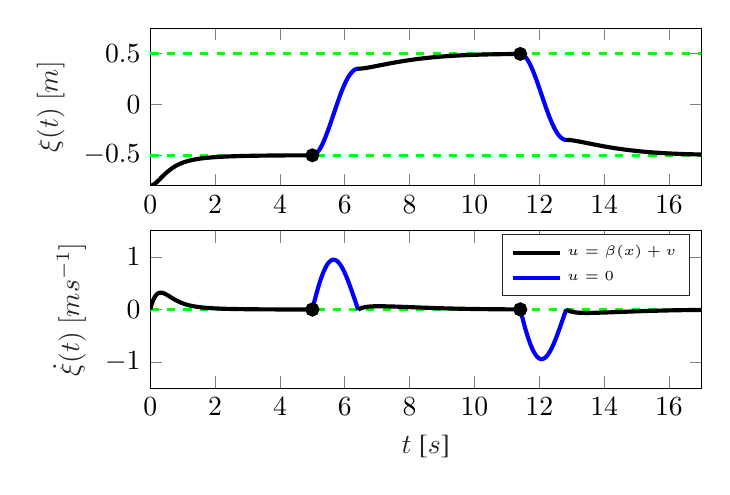
\begin{tikzpicture}

\begin{axis}[%
width=7cm,
height=2cm,
at={(0.758in,1.9in)},
scale only axis,
xmin=0,
xmax=17,
xlabel style={font=\color{white!15!black}},
xlabel={$t$ [$s$]},
ymin=-0.8,
ymax=0.75,
ylabel style={font=\color{white!15!black}},
ylabel={$\xi(t)~[m]$},
axis background/.style={fill=white},
legend style={legend cell align=left, align=left, draw=white!15!black}
]
\addplot [color=green, dashed, line width=1.0pt]
  table[row sep=crcr]{%
0	0.5\\
17.828	0.5\\
};
%\addlegendentry{data1}

\addplot [color=green, dashed, line width=1.0pt]
  table[row sep=crcr]{%
0	-0.5\\
17.828	-0.5\\
};
%\addlegendentry{data2}

\addplot [color=black, line width=1.5pt]
  table[row sep=crcr]{%
0	-0.8\\
0.00201272951242755	-0.799994961191618\\
0.00402545902485509	-0.799979912367723\\
0.00603818853728264	-0.799954954570979\\
0.00805091804971019	-0.799920188365097\\
0.0181145656118479	-0.799602716042907\\
0.0281782131739857	-0.799054842548506\\
0.0382418607361234	-0.798288597012259\\
0.0483055082982611	-0.797315700639723\\
0.0872883339796663	-0.79180232817447\\
0.126271159661072	-0.783973965721385\\
0.165253985342477	-0.774381288683226\\
0.204236811023882	-0.763501882011192\\
0.258325242573133	-0.747042020860754\\
0.312413674122383	-0.72976988716146\\
0.366502105671634	-0.712355838953056\\
0.420590537220884	-0.69531812887462\\
0.481968041514646	-0.676898302324055\\
0.543345545808408	-0.659689888119161\\
0.60472305010217	-0.643832734591055\\
0.666100554395931	-0.629420387260955\\
0.724027870722878	-0.61714861623052\\
0.781955187049825	-0.606081387447396\\
0.839882503376772	-0.596135540852008\\
0.897809819703719	-0.587228440080926\\
0.966381939079961	-0.577900541883002\\
1.0349540584562	-0.569737335894573\\
1.10352617783245	-0.562593329727953\\
1.17209829720869	-0.556334145892474\\
1.24444068335681	-0.550553176429767\\
1.31678306950493	-0.54550217235343\\
1.38912545565305	-0.541079788374854\\
1.46146784180118	-0.537189412277445\\
1.5338102279493	-0.533747712761737\\
1.60615261409742	-0.530698125658422\\
1.67849500024554	-0.527988925895292\\
1.75083738639366	-0.525569970593653\\
1.83596904357362	-0.52303674293993\\
1.92110070075358	-0.520801579050654\\
2.00623235793354	-0.518824975490308\\
2.0913640151135	-0.517065812797719\\
2.18740015096789	-0.515299213028131\\
2.28343628682228	-0.513739062989125\\
2.37947242267667	-0.512359606745628\\
2.47550855853105	-0.511132507072772\\
2.58940334197328	-0.509841944435238\\
2.7032981254155	-0.508712751315759\\
2.81719290885772	-0.507725193949768\\
2.93108769229994	-0.506855883378508\\
3.05608769229994	-0.506014933876777\\
3.18108769229994	-0.505281771732899\\
3.30608769229994	-0.504643252864409\\
3.43108769229994	-0.504084307800779\\
3.55608769229994	-0.503592377814803\\
3.68108769229994	-0.503161214961675\\
3.80608769229994	-0.502783544826694\\
3.93108769229994	-0.502451790226188\\
4.05608769229994	-0.502159488130832\\
4.18108769229994	-0.501902551685047\\
4.30608769229994	-0.501676794421557\\
4.43108769229994	-0.501478101249754\\
4.55608769229994	-0.501302911111012\\
4.68108769229994	-0.501148668049079\\
4.80608769229994	-0.501012909399428\\
4.93108769229994	-0.500893294150882\\
4.94831576922496	-0.500877951450443\\
4.96554384614997	-0.500862873825328\\
4.98277192307499	-0.500848056637506\\
5	-0.50083349533071\\
};
%\addlegendentry{data3}

\addplot [color=blue, line width=1.5pt]
  table[row sep=crcr]{%
5	-0.50083349533071\\
5.001	-0.50083138815981\\
5.002	-0.500826778512268\\
5.003	-0.500819667662055\\
5.004	-0.500810056895002\\
5.005	-0.500797947508799\\
5.006	-0.500783340812974\\
5.007	-0.500766238128885\\
5.008	-0.500746640789707\\
5.009	-0.500724550140417\\
5.01	-0.500699967537785\\
5.011	-0.500672894350357\\
5.012	-0.500643331958447\\
5.013	-0.500611281754122\\
5.014	-0.500576745141187\\
5.015	-0.500539723535175\\
5.016	-0.500500218363335\\
5.017	-0.500458231064615\\
5.018	-0.500413763089652\\
5.019	-0.500366815900759\\
5.02	-0.50031739097191\\
5.021	-0.500265489788728\\
5.022	-0.500211113848472\\
5.023	-0.500154264660022\\
5.024	-0.500094943743869\\
5.025	-0.500033152632097\\
5.026	-0.499968892868374\\
5.027	-0.499902166007936\\
5.028	-0.499832973617573\\
5.029	-0.499761317275618\\
5.03	-0.499687198571931\\
5.031	-0.499610619107885\\
5.032	-0.499531580496354\\
5.033	-0.499450084361699\\
5.034	-0.499366132339754\\
5.035	-0.499279726077809\\
5.036	-0.499190867234601\\
5.037	-0.499099557480297\\
5.038	-0.499005798496481\\
5.039	-0.49890959197614\\
5.04	-0.498810939623647\\
5.041	-0.498709843154752\\
5.042	-0.498606304296562\\
5.043	-0.498500324787532\\
5.044	-0.498391906377448\\
5.045	-0.49828105082741\\
5.046	-0.498167759909825\\
5.047	-0.498052035408383\\
5.048	-0.49793387911805\\
5.049	-0.497813292845051\\
5.05	-0.497690278406852\\
5.051	-0.497564837632153\\
5.052	-0.497436972360863\\
5.053	-0.497306684444096\\
5.054	-0.497173975744148\\
5.055	-0.497038848134484\\
5.056	-0.496901303499726\\
5.057	-0.496761343735636\\
5.058	-0.4966189707491\\
5.059	-0.496474186458115\\
5.06	-0.496326992791771\\
5.061	-0.49617739169024\\
5.062	-0.496025385104756\\
5.063	-0.495870974997602\\
5.064	-0.495714163342098\\
5.065	-0.495554952122578\\
5.066	-0.495393343334382\\
5.067	-0.495229338983836\\
5.068	-0.495062941088238\\
5.069	-0.494894151675843\\
5.07	-0.494722972785846\\
5.071	-0.494549406468367\\
5.072	-0.494373454784437\\
5.073	-0.494195119805977\\
5.074	-0.49401440361579\\
5.075	-0.493831308307538\\
5.076	-0.493645835985731\\
5.077	-0.493457988765707\\
5.078	-0.493267768773619\\
5.079	-0.49307517814642\\
5.08	-0.492880219031842\\
5.081	-0.492682893588384\\
5.082	-0.492483203985296\\
5.083	-0.492281152402559\\
5.084	-0.492076741030874\\
5.085	-0.491869972071641\\
5.086	-0.491660847736945\\
5.087	-0.491449370249538\\
5.088	-0.491235541842827\\
5.089	-0.491019364760851\\
5.09	-0.49080084125827\\
5.091	-0.490579973600343\\
5.092	-0.490356764062918\\
5.093	-0.490131214932411\\
5.094	-0.489903328505787\\
5.095	-0.489673107090551\\
5.096	-0.489440553004723\\
5.097	-0.489205668576827\\
5.098	-0.488968456145871\\
5.099	-0.48872891806133\\
5.1	-0.48848705668313\\
5.101	-0.488242874381633\\
5.102	-0.487996373537617\\
5.103	-0.487747556542257\\
5.104	-0.487496425797114\\
5.105	-0.487242983714113\\
5.106	-0.486987232715527\\
5.107	-0.48672917523396\\
5.108	-0.486468813712329\\
5.109	-0.486206150603849\\
5.11	-0.485941188372012\\
5.111	-0.485673929490572\\
5.112	-0.485404376443526\\
5.113	-0.485132531725098\\
5.114	-0.48485839783972\\
5.115	-0.484581977302018\\
5.116	-0.484303272636786\\
5.117	-0.484022286378978\\
5.118	-0.483739021073686\\
5.119	-0.483453479276118\\
5.12	-0.48316566355159\\
5.121	-0.482875576475498\\
5.122	-0.482583220633306\\
5.123	-0.482288598620527\\
5.124	-0.481991713042705\\
5.125	-0.481692566515396\\
5.126	-0.481391161664148\\
5.127	-0.481087501124491\\
5.128	-0.480781587541907\\
5.129	-0.480473423571822\\
5.13	-0.480163011879583\\
5.131	-0.479850355140439\\
5.132	-0.479535456039526\\
5.133	-0.479218317271846\\
5.134	-0.478898941542249\\
5.135	-0.478577331565415\\
5.136	-0.478253490065835\\
5.137	-0.477927419777795\\
5.138	-0.477599123445353\\
5.139	-0.477268603822325\\
5.14	-0.476935863672261\\
5.141	-0.476600905768431\\
5.142	-0.476263732893807\\
5.143	-0.475924347841039\\
5.144	-0.475582753412439\\
5.145	-0.475238952419964\\
5.146	-0.474892947685194\\
5.147	-0.474544742039317\\
5.148	-0.474194338323105\\
5.149	-0.473841739386897\\
5.15	-0.473486948090584\\
5.151	-0.473129967303583\\
5.152	-0.472770799904823\\
5.153	-0.472409448782724\\
5.154	-0.472045916835179\\
5.155	-0.471680206969531\\
5.156	-0.47131232210256\\
5.157	-0.470942265160457\\
5.158	-0.470570039078811\\
5.159	-0.470195646802585\\
5.16	-0.469819091286097\\
5.161	-0.469440375493005\\
5.162	-0.46905950239628\\
5.163	-0.468676474978194\\
5.164	-0.468291296230295\\
5.165	-0.467903969153392\\
5.166	-0.467514496757531\\
5.167	-0.467122882061978\\
5.168	-0.466729128095198\\
5.169	-0.466333237894836\\
5.17	-0.465935214507697\\
5.171	-0.465535060989727\\
5.172	-0.465132780405992\\
5.173	-0.464728375830658\\
5.174	-0.464321850346972\\
5.175	-0.463913207047241\\
5.176	-0.463502449032814\\
5.177	-0.46308957941406\\
5.178	-0.462674601310348\\
5.179	-0.462257517850029\\
5.18	-0.461838332170411\\
5.181	-0.461417047417748\\
5.182	-0.460993666747207\\
5.183	-0.460568193322861\\
5.184	-0.460140630317659\\
5.185	-0.459710980913409\\
5.186	-0.45927924830076\\
5.187	-0.458845435679179\\
5.188	-0.458409546256929\\
5.189	-0.457971583251053\\
5.19	-0.45753154988735\\
5.191	-0.457089449400357\\
5.192	-0.456645285033326\\
5.193	-0.456199060038205\\
5.194	-0.455750777675616\\
5.195	-0.455300441214836\\
5.196	-0.454848053933778\\
5.197	-0.454393619118963\\
5.198	-0.45393714006551\\
5.199	-0.453478620077105\\
5.2	-0.453018062465987\\
5.201	-0.452555470552923\\
5.202	-0.452090847667192\\
5.203	-0.451624197146558\\
5.204	-0.451155522337254\\
5.205	-0.450684826593958\\
5.206	-0.450212113279774\\
5.207	-0.449737385766211\\
5.208	-0.44926064743316\\
5.209	-0.448781901668874\\
5.21	-0.448301151869947\\
5.211	-0.447818401441293\\
5.212	-0.447333653796124\\
5.213	-0.446846912355932\\
5.214	-0.446358180550462\\
5.215	-0.445867461817695\\
5.216	-0.445374759603825\\
5.217	-0.444880077363241\\
5.218	-0.444383418558498\\
5.219	-0.443884786660306\\
5.22	-0.443384185147499\\
5.221	-0.442881617507019\\
5.222	-0.442377087233894\\
5.223	-0.441870597831214\\
5.224	-0.441362152810112\\
5.225	-0.440851755689741\\
5.226	-0.440339409997254\\
5.227	-0.439825119267781\\
5.228	-0.439308887044406\\
5.229	-0.438790716878149\\
5.23	-0.438270612327941\\
5.231	-0.437748576960605\\
5.232	-0.437224614350829\\
5.233	-0.436698728081153\\
5.234	-0.436170921741939\\
5.235	-0.435641198931352\\
5.236	-0.435109563255339\\
5.237	-0.434576018327607\\
5.238	-0.4340405677696\\
5.239	-0.433503215210478\\
5.24	-0.432963964287092\\
5.241	-0.432422818643969\\
5.242	-0.43187978193328\\
5.243	-0.431334857814829\\
5.244	-0.430788049956021\\
5.245	-0.430239362031845\\
5.246	-0.429688797724852\\
5.247	-0.429136360725132\\
5.248	-0.428582054730289\\
5.249	-0.428025883445425\\
5.25	-0.42746785058311\\
5.251	-0.426907959863368\\
5.252	-0.426346215013646\\
5.253	-0.4257826197688\\
5.254	-0.425217177871066\\
5.255	-0.424649893070042\\
5.256	-0.424080769122663\\
5.257	-0.423509809793179\\
5.258	-0.422937018853133\\
5.259	-0.422362400081341\\
5.26	-0.421785957263863\\
5.261	-0.421207694193988\\
5.262	-0.420627614672205\\
5.263	-0.420045722506185\\
5.264	-0.419462021510755\\
5.265	-0.418876515507879\\
5.266	-0.418289208326631\\
5.267	-0.417700103803177\\
5.268	-0.417109205780748\\
5.269	-0.41651651810962\\
5.27	-0.415922044647089\\
5.271	-0.415325789257452\\
5.272	-0.414727755811979\\
5.273	-0.414127948188896\\
5.274	-0.413526370273356\\
5.275	-0.412923025957421\\
5.276	-0.412317919140037\\
5.277	-0.41171105372701\\
5.278	-0.411102433630985\\
5.279	-0.410492062771425\\
5.28	-0.409879945074581\\
5.281	-0.409266084473477\\
5.282	-0.408650484907881\\
5.283	-0.408033150324285\\
5.284	-0.407414084675882\\
5.285	-0.40679329192254\\
5.286	-0.406170776030784\\
5.287	-0.405546540973766\\
5.288	-0.404920590731249\\
5.289	-0.404292929289579\\
5.29	-0.403663560641663\\
5.291	-0.403032488786945\\
5.292	-0.402399717731387\\
5.293	-0.401765251487438\\
5.294	-0.401129094074018\\
5.295	-0.400491249516491\\
5.296	-0.399851721846643\\
5.297	-0.399210515102658\\
5.298	-0.398567633329092\\
5.299	-0.397923080576857\\
5.3	-0.397276860903189\\
5.301	-0.39662897837163\\
5.302	-0.395979437052004\\
5.303	-0.395328241020388\\
5.304	-0.394675394359099\\
5.305	-0.394020901156661\\
5.306	-0.393364765507785\\
5.307	-0.392706991513346\\
5.308	-0.392047583280358\\
5.309	-0.391386544921953\\
5.31	-0.390723880557353\\
5.311	-0.39005959431185\\
5.312	-0.389393690316782\\
5.313	-0.388726172709509\\
5.314	-0.388057045633385\\
5.315	-0.387386313237744\\
5.316	-0.386713979677866\\
5.317	-0.386040049114958\\
5.318	-0.385364525716134\\
5.319	-0.384687413654381\\
5.32	-0.384008717108547\\
5.321	-0.383328440263308\\
5.322	-0.382646587309149\\
5.323	-0.381963162442338\\
5.324	-0.381278169864905\\
5.325	-0.380591613784614\\
5.326	-0.379903498414941\\
5.327	-0.379213827975053\\
5.328	-0.378522606689779\\
5.329	-0.377829838789588\\
5.33	-0.377135528510568\\
5.331	-0.376439680094396\\
5.332	-0.375742297788321\\
5.333	-0.375043385845134\\
5.334	-0.374342948523147\\
5.335	-0.373640990086169\\
5.336	-0.37293751480348\\
5.337	-0.37223252694981\\
5.338	-0.371526030805311\\
5.339	-0.370818030655537\\
5.34	-0.370108530791418\\
5.341	-0.369397535509233\\
5.342	-0.368685049110591\\
5.343	-0.367971075902405\\
5.344	-0.367255620196865\\
5.345	-0.366538686311418\\
5.346	-0.36582027856874\\
5.347	-0.365100401296717\\
5.348	-0.364379058828412\\
5.349	-0.363656255502052\\
5.35	-0.362931995660995\\
5.351	-0.362206283653707\\
5.352	-0.361479123833743\\
5.353	-0.360750520559716\\
5.354	-0.360020478195278\\
5.355	-0.359289001109091\\
5.356	-0.358556093674807\\
5.357	-0.357821760271041\\
5.358	-0.357086005281347\\
5.359	-0.356348833094194\\
5.36	-0.355610248102942\\
5.361	-0.354870254705817\\
5.362	-0.354128857305887\\
5.363	-0.353386060311035\\
5.364	-0.35264186813394\\
5.365	-0.351896285192048\\
5.366	-0.351149315907548\\
5.367	-0.350400964707351\\
5.368	-0.349651236023059\\
5.369	-0.348900134290949\\
5.37	-0.348147663951941\\
5.371	-0.347393829451576\\
5.372	-0.346638635239994\\
5.373	-0.345882085771906\\
5.374	-0.345124185506572\\
5.375	-0.344364938907772\\
5.376	-0.34360435044379\\
5.377	-0.342842424587379\\
5.378	-0.342079165815744\\
5.379	-0.341314578610515\\
5.38	-0.340548667457721\\
5.381	-0.339781436847767\\
5.382	-0.33901289127541\\
5.383	-0.338243035239732\\
5.384	-0.337471873244117\\
5.385	-0.336699409796227\\
5.386	-0.335925649407976\\
5.387	-0.335150596595505\\
5.388	-0.334374255879158\\
5.389	-0.333596631783458\\
5.39	-0.332817728837081\\
5.391	-0.332037551572833\\
5.392	-0.331256104527622\\
5.393	-0.330473392242438\\
5.394	-0.329689419262324\\
5.395	-0.328904190136352\\
5.396	-0.328117709417603\\
5.397	-0.327329981663135\\
5.398	-0.326541011433961\\
5.399	-0.325750803295029\\
5.4	-0.32495936181519\\
5.401	-0.324166691567175\\
5.402	-0.323372797127576\\
5.403	-0.322577683076813\\
5.404	-0.321781353999114\\
5.405	-0.320983814482489\\
5.406	-0.320185069118705\\
5.407	-0.319385122503263\\
5.408	-0.31858397923537\\
5.409	-0.317781643917915\\
5.41	-0.316978121157447\\
5.411	-0.316173415564147\\
5.412	-0.315367531751803\\
5.413	-0.314560474337789\\
5.414	-0.313752247943034\\
5.415	-0.312942857192005\\
5.416	-0.312132306712673\\
5.417	-0.311320601136496\\
5.418	-0.310507745098389\\
5.419	-0.309693743236703\\
5.42	-0.308878600193196\\
5.421	-0.308062320613011\\
5.422	-0.30724490914465\\
5.423	-0.30642637043995\\
5.424	-0.305606709154058\\
5.425	-0.304785929945403\\
5.426	-0.303964037475677\\
5.427	-0.303141036409803\\
5.428	-0.302316931415917\\
5.429	-0.301491727165337\\
5.43	-0.300665428332544\\
5.431	-0.29983803959515\\
5.432	-0.299009565633881\\
5.433	-0.298180011132544\\
5.434	-0.297349380778009\\
5.435	-0.296517679260181\\
5.436	-0.295684911271972\\
5.437	-0.294851081509283\\
5.438	-0.294016194670973\\
5.439	-0.293180255458837\\
5.44	-0.292343268577579\\
5.441	-0.29150523873479\\
5.442	-0.290666170640921\\
5.443	-0.289826069009256\\
5.444	-0.288984938555894\\
5.445	-0.288142783999714\\
5.446	-0.287299610062359\\
5.447	-0.286455421468207\\
5.448	-0.285610222944344\\
5.449	-0.284764019220545\\
5.45	-0.283916815029243\\
5.451	-0.283068615105506\\
5.452	-0.282219424187015\\
5.453	-0.281369247014034\\
5.454	-0.280518088329389\\
5.455	-0.279665952878441\\
5.456	-0.278812845409061\\
5.457	-0.277958770671608\\
5.458	-0.277103733418898\\
5.459	-0.276247738406184\\
5.46	-0.27539079039113\\
5.461	-0.274532894133786\\
5.462	-0.273674054396562\\
5.463	-0.272814275944203\\
5.464	-0.271953563543765\\
5.465	-0.27109192196459\\
5.466	-0.270229355978281\\
5.467	-0.269365870358675\\
5.468	-0.268501469881822\\
5.469	-0.267636159325956\\
5.47	-0.266769943471473\\
5.471	-0.265902827100903\\
5.472	-0.265034814998888\\
5.473	-0.264165911952157\\
5.474	-0.263296122749496\\
5.475	-0.262425452181731\\
5.476	-0.261553905041698\\
5.477	-0.260681486124216\\
5.478	-0.259808200226069\\
5.479	-0.258934052145975\\
5.48	-0.258059046684562\\
5.481	-0.257183188644348\\
5.482	-0.256306482829707\\
5.483	-0.255428934046852\\
5.484	-0.254550547103809\\
5.485	-0.253671326810387\\
5.486	-0.252791277978158\\
5.487	-0.25191040542043\\
5.488	-0.251028713952223\\
5.489	-0.250146208390245\\
5.49	-0.249262893552862\\
5.491	-0.24837877426008\\
5.492	-0.247493855333516\\
5.493	-0.246608141596373\\
5.494	-0.245721637873417\\
5.495	-0.244834348990952\\
5.496	-0.243946279776792\\
5.497	-0.24305743506024\\
5.498	-0.242167819672062\\
5.499	-0.24127743844446\\
5.5	-0.240386296211049\\
5.501	-0.239494397806833\\
5.502	-0.238601748068179\\
5.503	-0.23770835183279\\
5.504	-0.236814213939685\\
5.505	-0.23591933922917\\
5.506	-0.235023732542814\\
5.507	-0.234127398723427\\
5.508	-0.233230342615032\\
5.509	-0.232332569062839\\
5.51	-0.231434082913225\\
5.511	-0.230534889013706\\
5.512	-0.229634992212912\\
5.513	-0.228734397360563\\
5.514	-0.227833109307444\\
5.515	-0.226931132905382\\
5.516	-0.226028473007217\\
5.517	-0.225125134466782\\
5.518	-0.224221122138875\\
5.519	-0.223316440879235\\
5.52	-0.222411095544518\\
5.521	-0.221505090992272\\
5.522	-0.220598432080913\\
5.523	-0.219691123669696\\
5.524	-0.218783170618698\\
5.525	-0.217874577788787\\
5.526	-0.216965350041597\\
5.527	-0.21605549223951\\
5.528	-0.215145009245624\\
5.529	-0.214233905923732\\
5.53	-0.213322187138296\\
5.531	-0.212409857754424\\
5.532	-0.211496922637844\\
5.533	-0.210583386654878\\
5.534	-0.209669254672422\\
5.535	-0.208754531557915\\
5.536	-0.207839222179321\\
5.537	-0.2069233314051\\
5.538	-0.206006864104183\\
5.539	-0.205089825145952\\
5.54	-0.20417221940021\\
5.541	-0.20325405173716\\
5.542	-0.20233532702738\\
5.543	-0.201416050141797\\
5.544	-0.200496225951662\\
5.545	-0.199575859328531\\
5.546	-0.198654955144232\\
5.547	-0.197733518270846\\
5.548	-0.196811553580683\\
5.549	-0.195889065946254\\
5.55	-0.194966060240249\\
5.551	-0.194042541335512\\
5.552	-0.193118514105018\\
5.553	-0.192193983421844\\
5.554	-0.191268954159151\\
5.555	-0.190343431190153\\
5.556	-0.189417419388099\\
5.557	-0.188490923626243\\
5.558	-0.187563948777825\\
5.559	-0.186636499716041\\
5.56	-0.185708581314023\\
5.561	-0.184780198444813\\
5.562	-0.183851355981338\\
5.563	-0.182922058796388\\
5.564	-0.181992311762589\\
5.565	-0.181062119752381\\
5.566	-0.180131487637991\\
5.567	-0.179200420291413\\
5.568	-0.178268922584379\\
5.569	-0.177336999388339\\
5.57	-0.176404655574431\\
5.571	-0.175471896013466\\
5.572	-0.174538725575895\\
5.573	-0.173605149131788\\
5.574	-0.172671171550812\\
5.575	-0.171736797702204\\
5.576	-0.170802032454747\\
5.577	-0.169866880676748\\
5.578	-0.168931347236012\\
5.579	-0.167995436999819\\
5.58	-0.167059154834899\\
5.581	-0.166122505607409\\
5.582	-0.165185494182907\\
5.583	-0.164248125426331\\
5.584	-0.163310404201973\\
5.585	-0.162372335373455\\
5.586	-0.161433923803704\\
5.587	-0.160495174354933\\
5.588	-0.15955609188861\\
5.589	-0.158616681265439\\
5.59	-0.157676947345334\\
5.591	-0.156736894987398\\
5.592	-0.155796529049894\\
5.593	-0.154855854390224\\
5.594	-0.153914875864908\\
5.595	-0.152973598329555\\
5.596	-0.152032026638841\\
5.597	-0.151090165646488\\
5.598	-0.150148020205235\\
5.599	-0.14920559516682\\
5.6	-0.148262895381952\\
5.601	-0.147319925700288\\
5.602	-0.146376690970411\\
5.603	-0.145433196039804\\
5.604	-0.144489445754829\\
5.605	-0.143545444960702\\
5.606	-0.142601198501467\\
5.607	-0.141656711219977\\
5.608	-0.140711987957867\\
5.609	-0.139767033555531\\
5.61	-0.1388218528521\\
5.611	-0.137876450685416\\
5.612	-0.13693083189201\\
5.613	-0.135985001307079\\
5.614	-0.135038963764461\\
5.615	-0.134092724096612\\
5.616	-0.133146287134584\\
5.617	-0.132199657707998\\
5.618	-0.131252840645026\\
5.619	-0.130305840772362\\
5.62	-0.129358662915201\\
5.621	-0.128411311897218\\
5.622	-0.12746379254054\\
5.623	-0.126516109665726\\
5.624	-0.125568268091743\\
5.625	-0.124620272635942\\
5.626	-0.123672128114034\\
5.627	-0.122723839340071\\
5.628	-0.121775411126417\\
5.629	-0.120826848283727\\
5.63	-0.119878155620927\\
5.631	-0.118929337945185\\
5.632	-0.117980400061894\\
5.633	-0.117031346774644\\
5.634	-0.1160821828852\\
5.635	-0.115132913193481\\
5.636	-0.114183542497535\\
5.637	-0.113234075593516\\
5.638	-0.112284517275662\\
5.639	-0.111334872336272\\
5.64	-0.110385145565682\\
5.641	-0.109435341752242\\
5.642	-0.108485465682292\\
5.643	-0.107535522140145\\
5.644	-0.106585515908056\\
5.645	-0.105635451766205\\
5.646	-0.104685334492669\\
5.647	-0.103735168863406\\
5.648	-0.102784959652226\\
5.649	-0.101834711630771\\
5.65	-0.100884429568491\\
5.651	-0.0999341182326237\\
5.652	-0.098983782388169\\
5.653	-0.0980334267978677\\
5.654	-0.0970830562221785\\
5.655	-0.0961326754192551\\
5.656	-0.0951822891449244\\
5.657	-0.0942319021526632\\
5.658	-0.0932815191935751\\
5.659	-0.0923311450163692\\
5.66	-0.0913807843673368\\
5.661	-0.0904304419903294\\
5.662	-0.0894801226267348\\
5.663	-0.0885298310154567\\
5.664	-0.0875795718928907\\
5.665	-0.0866293499929027\\
5.666	-0.0856791700468059\\
5.667	-0.0847290367833387\\
5.668	-0.0837789549286425\\
5.669	-0.0828289292062394\\
5.67	-0.0818789643370093\\
5.671	-0.0809290650391687\\
5.672	-0.0799792360282472\\
5.673	-0.0790294820170659\\
5.674	-0.078079807715716\\
5.675	-0.0771302178315346\\
5.676	-0.0761807170690847\\
5.677	-0.0752313101301312\\
5.678	-0.074282001713621\\
5.679	-0.0733327965156584\\
5.68	-0.0723836992294845\\
5.681	-0.0714347145454556\\
5.682	-0.0704858471510201\\
5.683	-0.0695371017306966\\
5.684	-0.068588482966053\\
5.685	-0.0676399955356836\\
5.686	-0.0666916441151873\\
5.687	-0.0657434333771459\\
5.688	-0.0647953679911028\\
5.689	-0.0638474526235399\\
5.69	-0.0628996919378569\\
5.691	-0.0619520905943494\\
5.692	-0.0610046532501862\\
5.693	-0.0600573845593895\\
5.694	-0.0591102891728104\\
5.695	-0.0581633717381106\\
5.696	-0.0572166368997377\\
5.697	-0.0562700892989052\\
5.698	-0.0553237335735711\\
5.699	-0.0543775743584153\\
5.7	-0.0534316162848192\\
5.701	-0.0524858639808429\\
5.702	-0.0515403220712049\\
5.703	-0.0505949951772607\\
5.704	-0.04964988791698\\
5.705	-0.0487050049049264\\
5.706	-0.0477603507522364\\
5.707	-0.0468159300665964\\
5.708	-0.045871747452224\\
5.709	-0.044927807509844\\
5.71	-0.0439841148366686\\
5.711	-0.0430406740263765\\
5.712	-0.0420974896690902\\
5.713	-0.0411545663513569\\
5.714	-0.0402119086561252\\
5.715	-0.0392695211627254\\
5.716	-0.0383274084468481\\
5.717	-0.0373855750805235\\
5.718	-0.0364440256320989\\
5.719	-0.0355027646662197\\
5.72	-0.034561796743807\\
5.721	-0.0336211264220374\\
5.722	-0.0326807582543221\\
5.723	-0.031740696790285\\
5.724	-0.0308009465757431\\
5.725	-0.0298615121526855\\
5.726	-0.0289223980592517\\
5.727	-0.0279836088297118\\
5.728	-0.0270451489944456\\
5.729	-0.026107023079921\\
5.73	-0.025169235608675\\
5.731	-0.0242317910992912\\
5.732	-0.023294694066381\\
5.733	-0.022357949020561\\
5.734	-0.0214215604684348\\
5.735	-0.0204855329125704\\
5.736	-0.0195498708514806\\
5.737	-0.0186145787796028\\
5.738	-0.0176796611872781\\
5.739	-0.0167451225607312\\
5.74	-0.0158109673820496\\
5.741	-0.014877200129164\\
5.742	-0.0139438252758269\\
5.743	-0.0130108472915937\\
5.744	-0.0120782706418014\\
5.745	-0.0111460997875486\\
5.746	-0.0102143391856755\\
5.747	-0.00928299328874372\\
5.748	-0.00835206654501644\\
5.749	-0.00742156339843743\\
5.75	-0.00649148828861231\\
5.751	-0.00556184565078693\\
5.752	-0.00463263991582918\\
5.753	-0.00370387551020739\\
5.754	-0.00277555685597122\\
5.755	-0.00184768837073223\\
5.756	-0.000920274467642927\\
5.757	6.68044462262888e-06\\
5.758	0.000933171961888126\\
5.759	0.00185919568449575\\
5.76	0.00278474721732472\\
5.761	0.00370982216981178\\
5.762	0.00463441615597144\\
5.763	0.0055585247944138\\
5.764	0.00648214370836574\\
5.765	0.00740526852569016\\
5.766	0.00832789487890546\\
5.767	0.00925001840520382\\
5.768	0.0101716347464734\\
5.769	0.0110927395493152\\
5.77	0.0120133284650631\\
5.771	0.0129333971498045\\
5.772	0.0138529412643983\\
5.773	0.0147719564744945\\
5.774	0.0156904384505535\\
5.775	0.016608382867866\\
5.776	0.0175257854065708\\
5.777	0.0184426417516757\\
5.778	0.0193589475930751\\
5.779	0.0202746986255699\\
5.78	0.0211898905488866\\
5.781	0.0221045190676959\\
5.782	0.0230185798916319\\
5.783	0.0239320687353115\\
5.784	0.0248449813183527\\
5.785	0.0257573133653935\\
5.786	0.0266690606061114\\
5.787	0.0275802187752418\\
5.788	0.0284907836125964\\
5.789	0.0294007508630828\\
5.79	0.0303101162767225\\
5.791	0.0312188756086704\\
5.792	0.0321270246192321\\
5.793	0.0330345590738844\\
5.794	0.0339414747432919\\
5.795	0.034847767403327\\
5.796	0.0357534328350879\\
5.797	0.0366584668249169\\
5.798	0.0375628651644191\\
5.799	0.0384666236504805\\
5.8	0.0393697380852871\\
5.801	0.0402722042763421\\
5.802	0.0411740180364855\\
5.803	0.0420751751839116\\
5.804	0.0429756715421865\\
5.805	0.0438755029402681\\
5.806	0.0447746652125227\\
5.807	0.0456731541987439\\
5.808	0.0465709657441705\\
5.809	0.0474680956995043\\
5.81	0.0483645399209289\\
5.811	0.0492602942701261\\
5.812	0.0501553546142957\\
5.813	0.0510497168261723\\
5.814	0.0519433767840434\\
5.815	0.0528363303717672\\
5.816	0.0537285734787899\\
5.817	0.0546201020001652\\
5.818	0.0555109118365698\\
5.819	0.0564009988943225\\
5.82	0.0572903590854011\\
5.821	0.0581789883274605\\
5.822	0.0590668825438503\\
5.823	0.0599540376636316\\
5.824	0.0608404496215958\\
5.825	0.0617261143582802\\
5.826	0.0626110278199877\\
5.827	0.063495185958802\\
5.828	0.0643785847326066\\
5.829	0.065261220105101\\
5.83	0.0661430880458184\\
5.831	0.0670241845301432\\
5.832	0.0679045055393278\\
5.833	0.0687840470605097\\
5.834	0.0696628050867292\\
5.835	0.0705407756169459\\
5.836	0.0714179546560553\\
5.837	0.0722943382149071\\
5.838	0.073169922310322\\
5.839	0.0740447029651068\\
5.84	0.0749186762080734\\
5.841	0.0757918380740547\\
5.842	0.0766641846039215\\
5.843	0.0775357118445994\\
5.844	0.0784064158490856\\
5.845	0.0792762926764652\\
5.846	0.0801453383919281\\
5.847	0.081013549066786\\
5.848	0.0818809207784881\\
5.849	0.0827474496106383\\
5.85	0.083613131653012\\
5.851	0.0844779630015715\\
5.852	0.0853419397584835\\
5.853	0.0862050580321349\\
5.854	0.0870673139371488\\
5.855	0.0879287035944021\\
5.856	0.0887892231310399\\
5.857	0.0896488686804942\\
5.858	0.0905076363824969\\
5.859	0.091365522383099\\
5.86	0.0922225228346851\\
5.861	0.0930786338959894\\
5.862	0.0939338517321123\\
5.863	0.0947881725145364\\
5.864	0.0956415924211421\\
5.865	0.0964941076362229\\
5.866	0.0973457143505036\\
5.867	0.0981964087611527\\
5.868	0.0990461870718016\\
5.869	0.0998950454925577\\
5.87	0.100742980240022\\
5.871	0.101589987537303\\
5.872	0.102436063614033\\
5.873	0.103281204706386\\
5.874	0.10412540705709\\
5.875	0.104968666915443\\
5.876	0.105810980537329\\
5.877	0.106652344185236\\
5.878	0.107492754128266\\
5.879	0.108332206642155\\
5.88	0.109170698009286\\
5.881	0.110008224518705\\
5.882	0.110844782466137\\
5.883	0.111680368153999\\
5.884	0.112514977891418\\
5.885	0.113348607994241\\
5.886	0.114181254785057\\
5.887	0.115012914593209\\
5.888	0.115843583754805\\
5.889	0.116673258612739\\
5.89	0.117501935516704\\
5.891	0.118329610823205\\
5.892	0.119156280895574\\
5.893	0.119981942103987\\
5.894	0.120806590825479\\
5.895	0.121630223443954\\
5.896	0.122452836350206\\
5.897	0.123274425941928\\
5.898	0.12409498862373\\
5.899	0.124914520807152\\
5.9	0.125733018910681\\
5.901	0.12655047935976\\
5.902	0.127366898586809\\
5.903	0.128182273031234\\
5.904	0.128996599139445\\
5.905	0.129809873364867\\
5.906	0.130622092167958\\
5.907	0.131433252016219\\
5.908	0.132243349384212\\
5.909	0.133052380753572\\
5.91	0.13386034261302\\
5.911	0.13466723145838\\
5.912	0.135473043792591\\
5.913	0.136277776125721\\
5.914	0.137081424974981\\
5.915	0.137883986864739\\
5.916	0.138685458326536\\
5.917	0.139485835899093\\
5.918	0.140285116128335\\
5.919	0.141083295567394\\
5.92	0.14188037077663\\
5.921	0.142676338323641\\
5.922	0.14347119478328\\
5.923	0.144264936737663\\
5.924	0.145057560776189\\
5.925	0.145849063495546\\
5.926	0.146639441499733\\
5.927	0.147428691400064\\
5.928	0.148216809815191\\
5.929	0.149003793371109\\
5.93	0.149789638701172\\
5.931	0.150574342446108\\
5.932	0.151357901254032\\
5.933	0.152140311780455\\
5.934	0.152921570688302\\
5.935	0.153701674647921\\
5.936	0.154480620337099\\
5.937	0.155258404441073\\
5.938	0.156035023652543\\
5.939	0.156810474671687\\
5.94	0.157584754206171\\
5.941	0.158357858971161\\
5.942	0.15912978568934\\
5.943	0.159900531090917\\
5.944	0.16067009191364\\
5.945	0.16143846490281\\
5.946	0.162205646811292\\
5.947	0.162971634399529\\
5.948	0.163736424435553\\
5.949	0.164500013694996\\
5.95	0.165262398961107\\
5.951	0.166023577024761\\
5.952	0.166783544684469\\
5.953	0.167542298746397\\
5.954	0.16829983602437\\
5.955	0.169056153339891\\
5.956	0.169811247522148\\
5.957	0.17056511540803\\
5.958	0.171317753842136\\
5.959	0.172069159676788\\
5.96	0.172819329772043\\
5.961	0.173568260995706\\
5.962	0.174315950223339\\
5.963	0.175062394338273\\
5.964	0.175807590231625\\
5.965	0.176551534802302\\
5.966	0.177294224957017\\
5.967	0.178035657610302\\
5.968	0.178775829684513\\
5.969	0.17951473810985\\
5.97	0.180252379824361\\
5.971	0.18098875177396\\
5.972	0.181723850912432\\
5.973	0.182457674201447\\
5.974	0.183190218610573\\
5.975	0.183921481117286\\
5.976	0.184651458706978\\
5.977	0.185380148372975\\
5.978	0.186107547116541\\
5.979	0.186833651946892\\
5.98	0.187558459881209\\
5.981	0.188281967944645\\
5.982	0.189004173170338\\
5.983	0.189725072599423\\
5.984	0.190444663281039\\
5.985	0.191162942272345\\
5.986	0.191879906638525\\
5.987	0.192595553452805\\
5.988	0.193309879796457\\
5.989	0.194022882758813\\
5.99	0.194734559437277\\
5.991	0.195444906937333\\
5.992	0.196153922372556\\
5.993	0.196861602864621\\
5.994	0.197567945543317\\
5.995	0.198272947546554\\
5.996	0.198976606020376\\
5.997	0.199678918118967\\
5.998	0.200379881004665\\
5.999	0.201079491847972\\
6	0.20177774782756\\
6.001	0.202474646130288\\
6.002	0.203170183951204\\
6.003	0.203864358493562\\
6.004	0.204557166968826\\
6.005	0.205248606596683\\
6.006	0.205938674605055\\
6.007	0.206627368230103\\
6.008	0.207314684716242\\
6.009	0.208000621316146\\
6.01	0.208685175290762\\
6.011	0.209368343909317\\
6.012	0.210050124449328\\
6.013	0.210730514196611\\
6.014	0.211409510445292\\
6.015	0.212087110497816\\
6.016	0.212763311664952\\
6.017	0.213438111265811\\
6.018	0.214111506627847\\
6.019	0.21478349508687\\
6.02	0.215454073987054\\
6.021	0.216123240680949\\
6.022	0.216790992529484\\
6.023	0.217457326901982\\
6.024	0.218122241176167\\
6.025	0.218785732738171\\
6.026	0.219447798982545\\
6.027	0.220108437312267\\
6.028	0.220767645138752\\
6.029	0.22142541988186\\
6.03	0.222081758969901\\
6.031	0.22273665983965\\
6.032	0.223390119936353\\
6.033	0.224042136713732\\
6.034	0.224692707634001\\
6.035	0.225341830167867\\
6.036	0.225989501794541\\
6.037	0.226635720001748\\
6.038	0.227280482285736\\
6.039	0.227923786151278\\
6.04	0.228565629111689\\
6.041	0.229206008688826\\
6.042	0.229844922413102\\
6.043	0.230482367823493\\
6.044	0.231118342467541\\
6.045	0.231752843901369\\
6.046	0.232385869689687\\
6.047	0.233017417405794\\
6.048	0.233647484631595\\
6.049	0.234276068957603\\
6.05	0.234903167982947\\
6.051	0.235528779315383\\
6.052	0.236152900571296\\
6.053	0.236775529375714\\
6.054	0.237396663362313\\
6.055	0.238016300173421\\
6.056	0.23863443746003\\
6.057	0.239251072881804\\
6.058	0.239866204107081\\
6.059	0.240479828812886\\
6.06	0.241091944684935\\
6.061	0.241702549417643\\
6.062	0.242311640714132\\
6.063	0.242919216286237\\
6.064	0.243525273854512\\
6.065	0.244129811148242\\
6.066	0.244732825905444\\
6.067	0.245334315872876\\
6.068	0.245934278806048\\
6.069	0.24653271246922\\
6.07	0.247129614635418\\
6.071	0.247724983086435\\
6.072	0.248318815612841\\
6.073	0.248911110013986\\
6.074	0.24950186409801\\
6.075	0.250091075681849\\
6.076	0.250678742591239\\
6.077	0.251264862660727\\
6.078	0.251849433733671\\
6.079	0.252432453662252\\
6.08	0.253013920307481\\
6.081	0.253593831539198\\
6.082	0.254172185236086\\
6.083	0.254748979285673\\
6.084	0.25532421158434\\
6.085	0.255897880037326\\
6.086	0.256469982558734\\
6.087	0.257040517071537\\
6.088	0.257609481507586\\
6.089	0.258176873807613\\
6.09	0.258742691921238\\
6.091	0.259306933806976\\
6.092	0.259869597432239\\
6.093	0.260430680773349\\
6.094	0.260990181815534\\
6.095	0.261548098552942\\
6.096	0.262104428988642\\
6.097	0.262659171134631\\
6.098	0.263212323011838\\
6.099	0.263763882650133\\
6.1	0.264313848088329\\
6.101	0.264862217374186\\
6.102	0.265408988564424\\
6.103	0.265954159724717\\
6.104	0.266497728929707\\
6.105	0.267039694263007\\
6.106	0.267580053817203\\
6.107	0.268118805693864\\
6.108	0.268655948003542\\
6.109	0.269191478865779\\
6.11	0.269725396409116\\
6.111	0.27025769877109\\
6.112	0.270788384098244\\
6.113	0.271317450546132\\
6.114	0.271844896279321\\
6.115	0.272370719471398\\
6.116	0.272894918304972\\
6.117	0.273417490971681\\
6.118	0.273938435672198\\
6.119	0.27445775061623\\
6.12	0.274975434022527\\
6.121	0.275491484118885\\
6.122	0.276005899142151\\
6.123	0.276518677338225\\
6.124	0.277029816962067\\
6.125	0.277539316277701\\
6.126	0.278047173558218\\
6.127	0.278553387085778\\
6.128	0.279057955151619\\
6.129	0.279560876056057\\
6.13	0.280062148108492\\
6.131	0.280561769627412\\
6.132	0.281059738940395\\
6.133	0.281556054384114\\
6.134	0.282050714304341\\
6.135	0.28254371705595\\
6.136	0.283035061002923\\
6.137	0.28352474451835\\
6.138	0.284012765984434\\
6.139	0.284499123792496\\
6.14	0.284983816342976\\
6.141	0.28546684204544\\
6.142	0.28594819931858\\
6.143	0.286427886590217\\
6.144	0.286905902297308\\
6.145	0.287382244885946\\
6.146	0.287856912811365\\
6.147	0.288329904537941\\
6.148	0.288801218539199\\
6.149	0.28927085329781\\
6.15	0.289738807305601\\
6.151	0.290205079063553\\
6.152	0.290669667081805\\
6.153	0.291132569879658\\
6.154	0.291593785985578\\
6.155	0.292053313937196\\
6.156	0.292511152281314\\
6.157	0.292967299573906\\
6.158	0.293421754380121\\
6.159	0.293874515274285\\
6.16	0.294325580839906\\
6.161	0.294774949669673\\
6.162	0.295222620365458\\
6.163	0.295668591538326\\
6.164	0.296112861808527\\
6.165	0.296555429805504\\
6.166	0.296996294167895\\
6.167	0.297435453543535\\
6.168	0.297872906589458\\
6.169	0.298308651971897\\
6.17	0.298742688366288\\
6.171	0.299175014457275\\
6.172	0.299605628938705\\
6.173	0.300034530513636\\
6.174	0.300461717894336\\
6.175	0.300887189802287\\
6.176	0.301310944968182\\
6.177	0.301732982131934\\
6.178	0.302153300042671\\
6.179	0.302571897458741\\
6.18	0.302988773147714\\
6.181	0.303403925886382\\
6.182	0.30381735446076\\
6.183	0.30422905766609\\
6.184	0.304639034306839\\
6.185	0.305047283196705\\
6.186	0.305453803158613\\
6.187	0.305858593024722\\
6.188	0.306261651636419\\
6.189	0.306662977844327\\
6.19	0.307062570508302\\
6.191	0.307460428497438\\
6.192	0.307856550690063\\
6.193	0.308250935973742\\
6.194	0.308643583245281\\
6.195	0.309034491410724\\
6.196	0.309423659385356\\
6.197	0.3098110860937\\
6.198	0.310196770469524\\
6.199	0.310580711455838\\
6.2	0.310962908004895\\
6.201	0.31134335907819\\
6.202	0.311722063646464\\
6.203	0.312099020689704\\
6.204	0.312474229197138\\
6.205	0.312847688167245\\
6.206	0.313219396607746\\
6.207	0.313589353535611\\
6.208	0.313957557977056\\
6.209	0.314324008967544\\
6.21	0.314688705551785\\
6.211	0.315051646783736\\
6.212	0.315412831726602\\
6.213	0.315772259452836\\
6.214	0.316129929044138\\
6.215	0.316485839591455\\
6.216	0.316839990194983\\
6.217	0.317192379964164\\
6.218	0.317543008017686\\
6.219	0.317891873483487\\
6.22	0.318238975498749\\
6.221	0.318584313209901\\
6.222	0.31892788577262\\
6.223	0.319269692351826\\
6.224	0.319609732121684\\
6.225	0.319948004265606\\
6.226	0.320284507976247\\
6.227	0.320619242455504\\
6.228	0.320952206914519\\
6.229	0.321283400573676\\
6.23	0.321612822662599\\
6.231	0.321940472420154\\
6.232	0.322266349094447\\
6.233	0.322590451942822\\
6.234	0.322912780231862\\
6.235	0.323233333237386\\
6.236	0.323552110244452\\
6.237	0.32386911054735\\
6.238	0.324184333449606\\
6.239	0.324497778263978\\
6.24	0.324809444312456\\
6.241	0.325119330926261\\
6.242	0.325427437445842\\
6.243	0.325733763220877\\
6.244	0.326038307610271\\
6.245	0.326341069982153\\
6.246	0.326642049713876\\
6.247	0.326941246192016\\
6.248	0.327238658812368\\
6.249	0.327534286979948\\
6.25	0.327828130108989\\
6.251	0.328120187622938\\
6.252	0.328410458954459\\
6.253	0.328698943545426\\
6.254	0.328985640846924\\
6.255	0.329270550319247\\
6.256	0.329553671431896\\
6.257	0.329835003663575\\
6.258	0.330114546502192\\
6.259	0.330392299444857\\
6.26	0.330668261997876\\
6.261	0.330942433676754\\
6.262	0.331214814006188\\
6.263	0.331485402520068\\
6.264	0.331754198761475\\
6.265	0.332021202282675\\
6.266	0.332286412645123\\
6.267	0.332549829419453\\
6.268	0.332811452185481\\
6.269	0.3330712805322\\
6.27	0.33332931405778\\
6.271	0.333585552369562\\
6.272	0.333839995084058\\
6.273	0.334092641826948\\
6.274	0.334343492233074\\
6.275	0.334592545946443\\
6.276	0.334839802620221\\
6.277	0.335085261916727\\
6.278	0.335328923507438\\
6.279	0.335570787072978\\
6.28	0.335810852303121\\
6.281	0.336049118896783\\
6.282	0.336285586562024\\
6.283	0.336520255016039\\
6.284	0.336753123985163\\
6.285	0.336984193204859\\
6.286	0.33721346241972\\
6.287	0.337440931383463\\
6.288	0.337666599858931\\
6.289	0.337890467618081\\
6.29	0.33811253444199\\
6.291	0.338332800120842\\
6.292	0.338551264453933\\
6.293	0.338767927249663\\
6.294	0.338982788325531\\
6.295	0.339195847508137\\
6.296	0.339407104633173\\
6.297	0.339616559545421\\
6.298	0.33982421209875\\
6.299	0.340030062156111\\
6.3	0.340234109589535\\
6.301	0.340436354280126\\
6.302	0.340636796118061\\
6.303	0.340835435002581\\
6.304	0.341032270841993\\
6.305	0.341227303553661\\
6.306	0.341420533064005\\
6.307	0.341611959308493\\
6.308	0.341801582231642\\
6.309	0.34198940178701\\
6.31	0.342175417937193\\
6.311	0.342359630653819\\
6.312	0.342542039917548\\
6.313	0.342722645718063\\
6.314	0.342901448054067\\
6.315	0.343078446933278\\
6.316	0.343253642372428\\
6.317	0.343427034397252\\
6.318	0.34359862304249\\
6.319	0.343768408351877\\
6.32	0.343936390378143\\
6.321	0.344102569183003\\
6.322	0.344266944837156\\
6.323	0.344429517420281\\
6.324	0.344590287021028\\
6.325	0.344749253737016\\
6.326	0.344906417674828\\
6.327	0.345061778950004\\
6.328	0.345215337687039\\
6.329	0.345367094019376\\
6.33	0.345517048089398\\
6.331	0.345665200048429\\
6.332	0.345811550056727\\
6.333	0.345956098283474\\
6.334	0.346098844906775\\
6.335	0.346239790113652\\
6.336	0.346378934100039\\
6.337	0.346516277070776\\
6.338	0.346651819239602\\
6.339	0.346785560829151\\
6.34	0.346917502070949\\
6.341	0.347047643205403\\
6.342	0.347175984481798\\
6.343	0.347302526158294\\
6.344	0.347427268501914\\
6.345	0.347550211788546\\
6.346	0.347671356302931\\
6.347	0.347790702338658\\
6.348	0.347908250198161\\
6.349	0.348024000192712\\
6.35	0.348137952642414\\
6.351	0.348250107876194\\
6.352	0.348360466231801\\
6.353	0.348469028055795\\
6.354	0.348575793703544\\
6.355	0.348680763539217\\
6.356	0.348783937935778\\
6.357	0.34888531727498\\
6.358	0.348984901947357\\
6.359	0.349082692352218\\
6.36	0.349178688897646\\
6.361	0.349272892000481\\
6.362	0.349365302086325\\
6.363	0.349455919589525\\
6.364	0.349544744953177\\
6.365	0.34963177862911\\
6.366	0.349717021077883\\
6.367	0.349800472768783\\
6.368	0.349882134179809\\
6.369	0.349962005797674\\
6.37	0.350040088117791\\
6.371	0.350116381644272\\
6.372	0.350190886889919\\
6.373	0.350263604376215\\
6.374	0.35033453463332\\
6.375	0.350403678200064\\
6.376	0.350471035623936\\
6.377	0.350536607461082\\
6.378	0.350600394276295\\
6.379	0.350662396643008\\
6.38	0.35072261514329\\
6.381	0.350781050367832\\
6.382	0.350837702915948\\
6.383	0.350892573395559\\
6.384	0.350945662423196\\
6.385	0.350996970623981\\
6.386	0.351046498631629\\
6.387	0.351094247088437\\
6.388	0.351140216645274\\
6.389	0.351184407961578\\
6.39	0.351226821705346\\
6.391	0.351267458553126\\
6.392	0.351306319190011\\
6.393	0.351343404309631\\
6.394	0.351378714614141\\
6.395	0.351412250814221\\
6.396	0.351444013629063\\
6.397	0.351474003786362\\
6.398	0.351502222022313\\
6.399	0.3515286690816\\
6.4	0.351553345717386\\
6.401	0.351576252691311\\
6.402	0.351597390773478\\
6.403	0.351616760742447\\
6.404	0.351634363385229\\
6.405	0.351650199497275\\
6.406	0.351664269882468\\
6.407	0.351676575353118\\
6.408	0.351687116729948\\
6.409	0.351695894842092\\
6.41	0.351702910527081\\
6.411	0.351708164630841\\
6.412	0.351711658007676\\
6.413	0.351713391520268\\
};
%\addlegendentry{data4}

\addplot [color=black, line width=1.5pt]
  table[row sep=crcr]{%
6.413	0.351713391520268\\
6.42730885570975	0.351760697498142\\
6.44161771141949	0.351874948920672\\
6.45592656712924	0.35205151148703\\
6.47023542283898	0.352286033233259\\
6.51517744734551	0.353352231029928\\
6.56011947185204	0.354844795624168\\
6.60506149635856	0.356679595459083\\
6.65000352086509	0.358779242816386\\
6.69559714700642	0.361115524620325\\
6.74119077314774	0.36361815819057\\
6.78678439928907	0.366249865866127\\
6.8323780254304	0.368976195027982\\
6.88670805540013	0.372309315443092\\
6.94103808536987	0.375707260239703\\
6.99536811533961	0.379145014876719\\
7.04969814530934	0.382597978542932\\
7.11365261721454	0.386655218055554\\
7.17760708911974	0.390690015250083\\
7.24156156102494	0.394687928850088\\
7.30551603293014	0.398632829898123\\
7.38197671782709	0.403261064860015\\
7.45843740272405	0.407787376500753\\
7.53489808762101	0.412204232956827\\
7.61135877251796	0.416500047784615\\
7.70134213864231	0.421386858232834\\
7.79132550476665	0.426092939370141\\
7.881308870891	0.430617075996755\\
7.97129223701534	0.434950727526958\\
8.0720438339047	0.439567298973511\\
8.17279543079405	0.443945678062565\\
8.2735470276834	0.448092057512114\\
8.37429862457276	0.452002046961233\\
8.48225357766335	0.455925119791662\\
8.59020853075395	0.459591874214692\\
8.69816348384455	0.463015251702851\\
8.80611843693515	0.466196415876149\\
8.92128733479583	0.469325240039577\\
9.03645623265651	0.472206089720713\\
9.15162513051719	0.474856997838893\\
9.26679402837787	0.477284029545739\\
9.39145950708824	0.479666345284601\\
9.5161249857986	0.481823747637567\\
9.64079046450896	0.483777682415405\\
9.76545594321933	0.485537515852561\\
9.89045594321933	0.487117102950747\\
10.0154559432193	0.488535669702019\\
10.1404559432193	0.489809853041184\\
10.2654559432193	0.490949473347034\\
10.3904559432193	0.491964156984808\\
10.5154559432193	0.492870010536195\\
10.6404559432193	0.493678811754626\\
10.7654559432193	0.49439880434949\\
10.8904559432193	0.495037743420087\\
11.0154559432193	0.495605808645072\\
11.1404559432193	0.496110890244435\\
11.2654559432193	0.496559092004293\\
11.3023419574145	0.496681253027227\\
11.3392279716097	0.496799162261047\\
11.3761139858048	0.49691296158403\\
11.413	0.497022788413045\\
};
%\addlegendentry{data5}

\addplot [color=blue, line width=1.5pt]
  table[row sep=crcr]{%
11.413	0.497022788413045\\
11.414	0.497024533833223\\
11.415	0.497023793880453\\
11.416	0.497020569800809\\
11.417	0.49701486285216\\
11.418	0.497006674304158\\
11.419	0.496996005438225\\
11.42	0.496982857547541\\
11.421	0.496967231937032\\
11.422	0.496949129923356\\
11.423	0.496928552834893\\
11.424	0.49690550201173\\
11.425	0.496879978805651\\
11.426	0.496851984580123\\
11.427	0.496821520710282\\
11.428	0.496788588582924\\
11.429	0.496753189596487\\
11.43	0.496715325161045\\
11.431	0.496674996698287\\
11.432	0.496632205641511\\
11.433	0.496586953435609\\
11.434	0.496539241537052\\
11.435	0.496489071413878\\
11.436	0.49643644454568\\
11.437	0.496381362423593\\
11.438	0.496323826550277\\
11.439	0.49626383843991\\
11.44	0.496201399618169\\
11.441	0.496136511622219\\
11.442	0.496069176000699\\
11.443	0.495999394313711\\
11.444	0.495927168132803\\
11.445	0.495852499040957\\
11.446	0.495775388632574\\
11.447	0.495695838513463\\
11.448	0.495613850300827\\
11.449	0.495529425623244\\
11.45	0.495442566120662\\
11.451	0.495353273444377\\
11.452	0.495261549257023\\
11.453	0.495167395232558\\
11.454	0.49507081305625\\
11.455	0.49497180442466\\
11.456	0.494870371045632\\
11.457	0.494766514638277\\
11.458	0.494660236932958\\
11.459	0.494551539671277\\
11.46	0.494440424606061\\
11.461	0.494326893501344\\
11.462	0.494210948132358\\
11.463	0.494092590285516\\
11.464	0.493971821758395\\
11.465	0.493848644359726\\
11.466	0.493723059909376\\
11.467	0.493595070238336\\
11.468	0.493464677188704\\
11.469	0.493331882613669\\
11.47	0.493196688377503\\
11.471	0.493059096355536\\
11.472	0.49291910843415\\
11.473	0.492776726510761\\
11.474	0.4926319524938\\
11.475	0.492484788302705\\
11.476	0.4923352358679\\
11.477	0.492183297130785\\
11.478	0.492028974043715\\
11.479	0.49187226856999\\
11.48	0.491713182683836\\
11.481	0.491551718370393\\
11.482	0.491387877625696\\
11.483	0.491221662456662\\
11.484	0.491053074881075\\
11.485	0.490882116927569\\
11.486	0.490708790635611\\
11.487	0.49053309805549\\
11.488	0.490355041248296\\
11.489	0.490174622285909\\
11.49	0.489991843250981\\
11.491	0.489806706236918\\
11.492	0.48961921334787\\
11.493	0.489429366698708\\
11.494	0.489237168415015\\
11.495	0.489042620633064\\
11.496	0.488845725499807\\
11.497	0.488646485172855\\
11.498	0.488444901820463\\
11.499	0.488240977621516\\
11.5	0.488034714765511\\
11.501	0.48782611545254\\
11.502	0.487615181893275\\
11.503	0.48740191630895\\
11.504	0.487186320931348\\
11.505	0.486968398002782\\
11.506	0.486748149776077\\
11.507	0.486525578514559\\
11.508	0.48630068649203\\
11.509	0.486073475992761\\
11.51	0.485843949311468\\
11.511	0.485612108753298\\
11.512	0.485377956633814\\
11.513	0.485141495278975\\
11.514	0.484902727025121\\
11.515	0.484661654218954\\
11.516	0.484418279217526\\
11.517	0.484172604388217\\
11.518	0.483924632108719\\
11.519	0.483674364767023\\
11.52	0.483421804761394\\
11.521	0.483166954500364\\
11.522	0.482909816402704\\
11.523	0.482650392897418\\
11.524	0.482388686423714\\
11.525	0.482124699430998\\
11.526	0.481858434378847\\
11.527	0.481589893737\\
11.528	0.481319079985332\\
11.529	0.481045995613846\\
11.53	0.480770643122647\\
11.531	0.480493025021928\\
11.532	0.480213143831956\\
11.533	0.479931002083047\\
11.534	0.479646602315553\\
11.535	0.479359947079845\\
11.536	0.479071038936291\\
11.537	0.478779880455244\\
11.538	0.47848647421702\\
11.539	0.478190822811878\\
11.54	0.477892928840009\\
11.541	0.477592794911514\\
11.542	0.477290423646384\\
11.543	0.476985817674486\\
11.544	0.476678979635543\\
11.545	0.476369912179115\\
11.546	0.476058617964582\\
11.547	0.475745099661127\\
11.548	0.475429359947716\\
11.549	0.475111401513079\\
11.55	0.474791227055693\\
11.551	0.474468839283764\\
11.552	0.474144240915208\\
11.553	0.473817434677634\\
11.554	0.47348842330832\\
11.555	0.473157209554204\\
11.556	0.472823796171855\\
11.557	0.472488185927463\\
11.558	0.472150381596815\\
11.559	0.471810385965279\\
11.56	0.471468201827784\\
11.561	0.471123831988801\\
11.562	0.470777279262327\\
11.563	0.470428546471863\\
11.564	0.470077636450394\\
11.565	0.469724552040375\\
11.566	0.469369296093709\\
11.567	0.469011871471728\\
11.568	0.468652281045175\\
11.569	0.468290527694181\\
11.57	0.467926614308254\\
11.571	0.467560543786252\\
11.572	0.467192319036368\\
11.573	0.46682194297611\\
11.574	0.46644941853228\\
11.575	0.466074748640958\\
11.576	0.465697936247479\\
11.577	0.465318984306417\\
11.578	0.464937895781565\\
11.579	0.464554673645912\\
11.58	0.464169320881627\\
11.581	0.463781840480041\\
11.582	0.463392235441623\\
11.583	0.463000508775964\\
11.584	0.462606663501754\\
11.585	0.462210702646767\\
11.586	0.461812629247837\\
11.587	0.461412446350841\\
11.588	0.461010157010678\\
11.589	0.460605764291248\\
11.59	0.460199271265437\\
11.591	0.459790681015092\\
11.592	0.459379996631001\\
11.593	0.458967221212878\\
11.594	0.458552357869339\\
11.595	0.458135409717883\\
11.596	0.457716379884873\\
11.597	0.457295271505513\\
11.598	0.456872087723832\\
11.599	0.456446831692661\\
11.6	0.456019506573612\\
11.601	0.455590115537063\\
11.602	0.455158661762131\\
11.603	0.454725148436657\\
11.604	0.454289578757181\\
11.605	0.453851955928928\\
11.606	0.453412283165782\\
11.607	0.452970563690266\\
11.608	0.452526800733527\\
11.609	0.452080997535308\\
11.61	0.451633157343932\\
11.611	0.451183283416284\\
11.612	0.450731379017781\\
11.613	0.450277447422364\\
11.614	0.449821491912466\\
11.615	0.449363515778998\\
11.616	0.448903522321328\\
11.617	0.448441514847256\\
11.618	0.447977496672998\\
11.619	0.447511471123163\\
11.62	0.447043441530731\\
11.621	0.446573411237037\\
11.622	0.446101383591743\\
11.623	0.445627361952824\\
11.624	0.44515134968654\\
11.625	0.444673350167424\\
11.626	0.444193366778251\\
11.627	0.443711402910025\\
11.628	0.443227461961955\\
11.629	0.442741547341432\\
11.63	0.442253662464009\\
11.631	0.441763810753384\\
11.632	0.441271995641372\\
11.633	0.440778220567888\\
11.634	0.440282488980925\\
11.635	0.439784804336533\\
11.636	0.439285170098797\\
11.637	0.438783589739816\\
11.638	0.43828006673968\\
11.639	0.437774604586452\\
11.64	0.437267206776145\\
11.641	0.436757876812698\\
11.642	0.436246618207959\\
11.643	0.435733434481661\\
11.644	0.4352183291614\\
11.645	0.434701305782615\\
11.646	0.434182367888565\\
11.647	0.433661519030307\\
11.648	0.433138762766678\\
11.649	0.432614102664269\\
11.65	0.432087542297404\\
11.651	0.431559085248122\\
11.652	0.43102873510615\\
11.653	0.430496495468885\\
11.654	0.429962369941369\\
11.655	0.429426362136272\\
11.656	0.428888475673865\\
11.657	0.428348714182001\\
11.658	0.427807081296092\\
11.659	0.427263580659087\\
11.66	0.426718215921451\\
11.661	0.426170990741143\\
11.662	0.425621908783593\\
11.663	0.425070973721678\\
11.664	0.424518189235706\\
11.665	0.423963559013388\\
11.666	0.423407086749818\\
11.667	0.422848776147451\\
11.668	0.422288630916081\\
11.669	0.421726654772818\\
11.67	0.421162851442066\\
11.671	0.420597224655501\\
11.672	0.420029778152051\\
11.673	0.419460515677866\\
11.674	0.418889440986306\\
11.675	0.418316557837912\\
11.676	0.417741870000384\\
11.677	0.417165381248561\\
11.678	0.416587095364398\\
11.679	0.416007016136941\\
11.68	0.415425147362307\\
11.681	0.414841492843663\\
11.682	0.414256056391199\\
11.683	0.413668841822108\\
11.684	0.413079852960565\\
11.685	0.4124890936377\\
11.686	0.411896567691581\\
11.687	0.411302278967185\\
11.688	0.410706231316382\\
11.689	0.410108428597907\\
11.69	0.40950887467734\\
11.691	0.408907573427081\\
11.692	0.408304528726332\\
11.693	0.407699744461067\\
11.694	0.407093224524016\\
11.695	0.406484972814638\\
11.696	0.4058749932391\\
11.697	0.405263289710253\\
11.698	0.404649866147611\\
11.699	0.404034726477326\\
11.7	0.403417874632164\\
11.701	0.402799314551486\\
11.702	0.402179050181223\\
11.703	0.401557085473852\\
11.704	0.400933424388374\\
11.705	0.40030807089029\\
11.706	0.39968102895158\\
11.707	0.399052302550678\\
11.708	0.398421895672449\\
11.709	0.397789812308168\\
11.71	0.397156056455492\\
11.711	0.396520632118445\\
11.712	0.395883543307384\\
11.713	0.395244794038986\\
11.714	0.394604388336218\\
11.715	0.393962330228319\\
11.716	0.393318623750769\\
11.717	0.392673272945275\\
11.718	0.392026281859741\\
11.719	0.391377654548248\\
11.72	0.390727395071029\\
11.721	0.390075507494446\\
11.722	0.389421995890967\\
11.723	0.388766864339142\\
11.724	0.388110116923582\\
11.725	0.387451757734929\\
11.726	0.386791790869843\\
11.727	0.386130220430966\\
11.728	0.385467050526912\\
11.729	0.38480228527223\\
11.73	0.384135928787393\\
11.731	0.383467985198762\\
11.732	0.382798458638575\\
11.733	0.382127353244914\\
11.734	0.381454673161684\\
11.735	0.380780422538593\\
11.736	0.380104605531122\\
11.737	0.379427226300508\\
11.738	0.378748289013715\\
11.739	0.378067797843412\\
11.74	0.377385756967951\\
11.741	0.376702170571342\\
11.742	0.376017042843229\\
11.743	0.375330377978864\\
11.744	0.37464218017909\\
11.745	0.373952453650309\\
11.746	0.373261202604464\\
11.747	0.372568431259013\\
11.748	0.371874143836906\\
11.749	0.371178344566559\\
11.75	0.370481037681833\\
11.751	0.369782227422007\\
11.752	0.369081918031759\\
11.753	0.368380113761135\\
11.754	0.367676818865533\\
11.755	0.366972037605673\\
11.756	0.366265774247574\\
11.757	0.365558033062534\\
11.758	0.3648488183271\\
11.759	0.364138134323051\\
11.76	0.363425985337367\\
11.761	0.362712375662208\\
11.762	0.361997309594893\\
11.763	0.361280791437871\\
11.764	0.360562825498698\\
11.765	0.359843416090016\\
11.766	0.359122567529526\\
11.767	0.358400284139963\\
11.768	0.357676570249076\\
11.769	0.356951430189601\\
11.77	0.356224868299235\\
11.771	0.355496888920617\\
11.772	0.354767496401298\\
11.773	0.354036695093723\\
11.774	0.353304489355201\\
11.775	0.352570883547883\\
11.776	0.351835882038741\\
11.777	0.351099489199537\\
11.778	0.350361709406806\\
11.779	0.349622547041826\\
11.78	0.348882006490597\\
11.781	0.348140092143815\\
11.782	0.34739680839685\\
11.783	0.346652159649718\\
11.784	0.345906150307062\\
11.785	0.34515878477812\\
11.786	0.34441006747671\\
11.787	0.343660002821197\\
11.788	0.342908595234474\\
11.789	0.342155849143937\\
11.79	0.341401768981458\\
11.791	0.340646359183363\\
11.792	0.339889624190407\\
11.793	0.33913156844775\\
11.794	0.338372196404931\\
11.795	0.337611512515845\\
11.796	0.336849521238719\\
11.797	0.336086227036085\\
11.798	0.335321634374759\\
11.799	0.334555747725815\\
11.8	0.333788571564558\\
11.801	0.333020110370505\\
11.802	0.332250368627354\\
11.803	0.331479350822967\\
11.804	0.330707061449336\\
11.805	0.329933505002569\\
11.806	0.329158685982857\\
11.807	0.328382608894454\\
11.808	0.327605278245651\\
11.809	0.326826698548752\\
11.81	0.326046874320048\\
11.811	0.325265810079795\\
11.812	0.324483510352187\\
11.813	0.323699979665332\\
11.814	0.32291522255123\\
11.815	0.322129243545742\\
11.816	0.321342047188574\\
11.817	0.320553638023246\\
11.818	0.319764020597068\\
11.819	0.318973199461119\\
11.82	0.318181179170219\\
11.821	0.317387964282905\\
11.822	0.316593559361409\\
11.823	0.315797968971627\\
11.824	0.315001197683103\\
11.825	0.314203250068997\\
11.826	0.313404130706063\\
11.827	0.312603844174627\\
11.828	0.311802395058558\\
11.829	0.310999787945244\\
11.83	0.310196027425571\\
11.831	0.309391118093893\\
11.832	0.308585064548013\\
11.833	0.307777871389153\\
11.834	0.306969543221932\\
11.835	0.306160084654342\\
11.836	0.305349500297722\\
11.837	0.304537794766731\\
11.838	0.303724972679328\\
11.839	0.302911038656746\\
11.84	0.302095997323463\\
11.841	0.301279853307183\\
11.842	0.300462611238809\\
11.843	0.299644275752416\\
11.844	0.298824851485229\\
11.845	0.298004343077599\\
11.846	0.297182755172975\\
11.847	0.296360092417881\\
11.848	0.295536359461893\\
11.849	0.294711560957611\\
11.85	0.293885701560635\\
11.851	0.293058785929543\\
11.852	0.292230818725862\\
11.853	0.291401804614047\\
11.854	0.290571748261453\\
11.855	0.289740654338315\\
11.856	0.288908527517715\\
11.857	0.288075372475568\\
11.858	0.287241193890586\\
11.859	0.286405996444262\\
11.86	0.285569784820841\\
11.861	0.284732563707296\\
11.862	0.283894337793304\\
11.863	0.283055111771219\\
11.864	0.28221489033605\\
11.865	0.281373678185434\\
11.866	0.280531480019613\\
11.867	0.279688300541408\\
11.868	0.278844144456194\\
11.869	0.277999016471877\\
11.87	0.277152921298865\\
11.871	0.276305863650051\\
11.872	0.275457848240778\\
11.873	0.274608879788822\\
11.874	0.273758963014367\\
11.875	0.272908102639973\\
11.876	0.272056303390561\\
11.877	0.271203569993379\\
11.878	0.270349907177985\\
11.879	0.269495319676216\\
11.88	0.268639812222169\\
11.881	0.267783389552171\\
11.882	0.266926056404756\\
11.883	0.266067817520642\\
11.884	0.265208677642704\\
11.885	0.264348641515949\\
11.886	0.263487713887496\\
11.887	0.262625899506543\\
11.888	0.261763203124348\\
11.889	0.260899629494205\\
11.89	0.260035183371414\\
11.891	0.259169869513261\\
11.892	0.258303692678992\\
11.893	0.257436657629786\\
11.894	0.256568769128734\\
11.895	0.255700031940811\\
11.896	0.254830450832852\\
11.897	0.253960030573529\\
11.898	0.253088775933325\\
11.899	0.252216691684508\\
11.9	0.251343782601108\\
11.901	0.250470053458892\\
11.902	0.249595509035339\\
11.903	0.248720154109615\\
11.904	0.247843993462549\\
11.905	0.246967031876606\\
11.906	0.246089274135868\\
11.907	0.245210725026\\
11.908	0.244331389334235\\
11.909	0.243451271849342\\
11.91	0.242570377361607\\
11.911	0.241688710662803\\
11.912	0.240806276546169\\
11.913	0.239923079806384\\
11.914	0.239039125239543\\
11.915	0.23815441764313\\
11.916	0.237268961815996\\
11.917	0.236382762558334\\
11.918	0.235495824671653\\
11.919	0.234608152958754\\
11.92	0.233719752223707\\
11.921	0.232830627271823\\
11.922	0.23194078290963\\
11.923	0.231050223944853\\
11.924	0.230158955186383\\
11.925	0.229266981444256\\
11.926	0.228374307529629\\
11.927	0.227480938254752\\
11.928	0.226586878432946\\
11.929	0.225692132878578\\
11.93	0.224796706407036\\
11.931	0.223900603834706\\
11.932	0.223003829978945\\
11.933	0.222106389658055\\
11.934	0.221208287691267\\
11.935	0.220309528898704\\
11.936	0.219410118101366\\
11.937	0.218510060121103\\
11.938	0.217609359780588\\
11.939	0.216708021903296\\
11.94	0.215806051313475\\
11.941	0.214903452836127\\
11.942	0.21400023129698\\
11.943	0.213096391522463\\
11.944	0.212191938339685\\
11.945	0.211286876576407\\
11.946	0.210381211061018\\
11.947	0.209474946622513\\
11.948	0.208568088090466\\
11.949	0.207660640295008\\
11.95	0.206752608066799\\
11.951	0.205843996237007\\
11.952	0.204934809637281\\
11.953	0.204025053099731\\
11.954	0.203114731456897\\
11.955	0.20220384954173\\
11.956	0.201292412187566\\
11.957	0.2003804242281\\
11.958	0.199467890497364\\
11.959	0.198554815829702\\
11.96	0.197641205059745\\
11.961	0.196727063022388\\
11.962	0.195812394552763\\
11.963	0.194897204486218\\
11.964	0.193981497658291\\
11.965	0.193065278904686\\
11.966	0.192148553061248\\
11.967	0.191231324963941\\
11.968	0.190313599448821\\
11.969	0.189395381352014\\
11.97	0.18847667550969\\
11.971	0.187557486758039\\
11.972	0.186637819933249\\
11.973	0.18571767987148\\
11.974	0.184797071408839\\
11.975	0.183875999381358\\
11.976	0.182954468624969\\
11.977	0.182032483975479\\
11.978	0.181110050268547\\
11.979	0.180187172339659\\
11.98	0.179263855024105\\
11.981	0.178340103156954\\
11.982	0.17741592157303\\
11.983	0.17649131510689\\
11.984	0.175566288592795\\
11.985	0.174640846864693\\
11.986	0.173714994756187\\
11.987	0.17278873710052\\
11.988	0.171862078730542\\
11.989	0.170935024478691\\
11.99	0.170007579176971\\
11.991	0.169079747656923\\
11.992	0.168151534749604\\
11.993	0.167222945285561\\
11.994	0.166293984094813\\
11.995	0.165364656006817\\
11.996	0.164434965850455\\
11.997	0.163504918454001\\
11.998	0.162574518645105\\
11.999	0.161643771250762\\
12	0.160712681097294\\
12.001	0.159781253010322\\
12.002	0.158849491814745\\
12.003	0.157917402334717\\
12.004	0.156984989393617\\
12.005	0.156052257814035\\
12.006	0.155119212417738\\
12.007	0.154185858025657\\
12.008	0.153252199457853\\
12.009	0.1523182415335\\
12.01	0.15138398907086\\
12.011	0.150449446887257\\
12.012	0.149514619799058\\
12.013	0.148579512621643\\
12.014	0.147644130169387\\
12.015	0.146708477255636\\
12.016	0.145772558692678\\
12.017	0.144836379291728\\
12.018	0.143899943862895\\
12.019	0.142963257215167\\
12.02	0.142026324156383\\
12.021	0.141089149493209\\
12.022	0.140151738031118\\
12.023	0.139214094574364\\
12.024	0.138276223925957\\
12.025	0.137338130887645\\
12.026	0.136399820259886\\
12.027	0.135461296841826\\
12.028	0.134522565431275\\
12.029	0.133583630824686\\
12.03	0.132644497817129\\
12.031	0.131705171202269\\
12.032	0.130765655772342\\
12.033	0.129825956318134\\
12.034	0.128886077628954\\
12.035	0.127946024492614\\
12.036	0.127005801695405\\
12.037	0.126065414022074\\
12.038	0.125124866255798\\
12.039	0.124184163178166\\
12.04	0.123243309569152\\
12.041	0.122302310207093\\
12.042	0.121361169868665\\
12.043	0.120419893328863\\
12.044	0.119478485360975\\
12.045	0.118536950736559\\
12.046	0.117595294225424\\
12.047	0.1166535205956\\
12.048	0.115711634613321\\
12.049	0.114769641043001\\
12.05	0.113827544647208\\
12.051	0.112885350186646\\
12.052	0.111943062420126\\
12.053	0.11100068610455\\
12.054	0.110058225994883\\
12.055	0.109115686844131\\
12.056	0.108173073403323\\
12.057	0.107230390421479\\
12.058	0.106287642645598\\
12.059	0.105344834820627\\
12.06	0.104401971689441\\
12.061	0.103459057992821\\
12.062	0.102516098469434\\
12.063	0.101573097855803\\
12.064	0.100630060886291\\
12.065	0.0996869922930753\\
12.066	0.0987438968061265\\
12.067	0.0978007791531848\\
12.068	0.0968576440597379\\
12.069	0.0959144962489988\\
12.07	0.0949713404418833\\
12.071	0.0940281813569862\\
12.072	0.0930850237105611\\
12.073	0.0921418722164962\\
12.074	0.0911987315862934\\
12.075	0.0902556065290438\\
12.076	0.089312501751408\\
12.077	0.0883694219575919\\
12.078	0.087426371849325\\
12.079	0.0864833561258384\\
12.08	0.0855403794838417\\
12.081	0.084597446617502\\
12.082	0.0836545622184209\\
12.083	0.0827117309756121\\
12.084	0.0817689575754804\\
12.085	0.0808262467017985\\
12.086	0.0798836030356846\\
12.087	0.0789410312555825\\
12.088	0.0779985360372364\\
12.089	0.0770561220536714\\
12.09	0.0761137939751702\\
12.091	0.0751715564692522\\
12.092	0.0742294142006501\\
12.093	0.0732873718312888\\
12.094	0.0723454340202641\\
12.095	0.0714036054238196\\
12.096	0.0704618906953255\\
12.097	0.0695202944852569\\
12.098	0.0685788214411719\\
12.099	0.0676374762076892\\
12.1	0.0666962634264672\\
12.101	0.0657551877361821\\
12.102	0.0648142537725059\\
12.103	0.0638734661680846\\
12.104	0.0629328295525177\\
12.105	0.0619923485523345\\
12.106	0.0610520277909752\\
12.107	0.0601118718887661\\
12.108	0.0591718854629016\\
12.109	0.0582320731274198\\
12.11	0.0572924394931822\\
12.111	0.0563529891678527\\
12.112	0.055413726755875\\
12.113	0.0544746568584525\\
12.114	0.0535357840735255\\
12.115	0.0525971129957511\\
12.116	0.0516586482164814\\
12.117	0.050720394323742\\
12.118	0.0497823559022105\\
12.119	0.0488445375331966\\
12.12	0.0479069437946185\\
12.121	0.0469695792609848\\
12.122	0.0460324485033706\\
12.123	0.0450955560893975\\
12.124	0.044158906583213\\
12.125	0.0432225045454684\\
12.126	0.0422863545332986\\
12.127	0.0413504611003\\
12.128	0.0404148287965107\\
12.129	0.0394794621683889\\
12.13	0.0385443657587928\\
12.131	0.0376095441069574\\
12.132	0.0366750017484768\\
12.133	0.0357407432152807\\
12.134	0.0348067730356153\\
12.135	0.0338730957340216\\
12.136	0.0329397158313145\\
12.137	0.0320066378445629\\
12.138	0.0310738662870685\\
12.139	0.0301414056683449\\
12.14	0.0292092604940976\\
12.141	0.0282774352662026\\
12.142	0.027345934482686\\
12.143	0.0264147626377044\\
12.144	0.0254839242215228\\
12.145	0.0245534237204959\\
12.146	0.023623265617045\\
12.147	0.0226934543896411\\
12.148	0.0217639945127812\\
12.149	0.0208348904569697\\
12.15	0.0199061466886979\\
12.151	0.0189777676704231\\
12.152	0.018049757860549\\
12.153	0.0171221217134045\\
12.154	0.0161948636792247\\
12.155	0.0152679882041294\\
12.156	0.0143414997301042\\
12.157	0.0134154026949794\\
12.158	0.0124897015324103\\
12.159	0.0115644006718569\\
12.16	0.0106395045385642\\
12.161	0.00971501755354217\\
12.162	0.00879094413354512\\
12.163	0.00786728869105287\\
12.164	0.00694405563424933\\
12.165	0.00602124936700441\\
12.166	0.0050988742888525\\
12.167	0.00417693479497348\\
12.168	0.00325543527617338\\
12.169	0.00233438011886353\\
12.17	0.00141377370504127\\
12.171	0.000493620412270762\\
12.172	-0.000426075386337674\\
12.173	-0.00134530932214601\\
12.174	-0.00226407703100885\\
12.175	-0.00318237415329365\\
12.176	-0.00410019633389833\\
12.177	-0.00501753922227249\\
12.178	-0.00593439847243649\\
12.179	-0.00685076974300079\\
12.18	-0.00776664869718424\\
12.181	-0.00868203100283605\\
12.182	-0.00959691233245272\\
12.183	-0.0105112883631977\\
12.184	-0.0114251547769225\\
12.185	-0.0123385072601837\\
12.186	-0.0132513415042633\\
12.187	-0.0141636532051874\\
12.188	-0.0150754380637463\\
12.189	-0.0159866917855122\\
12.19	-0.0168974100808593\\
12.191	-0.0178075886649827\\
12.192	-0.0187172232579169\\
12.193	-0.0196263095845554\\
12.194	-0.0205348433746691\\
12.195	-0.0214428203629257\\
12.196	-0.0223502362889083\\
12.197	-0.0232570868971344\\
12.198	-0.0241633679370741\\
12.199	-0.0250690751631698\\
12.2	-0.0259742043348549\\
12.201	-0.0268787512165709\\
12.202	-0.0277827115777884\\
12.203	-0.028686081193024\\
12.204	-0.0295888558418599\\
12.205	-0.0304910313089615\\
12.206	-0.0313926033840973\\
12.207	-0.0322935678621559\\
12.208	-0.0331939205431654\\
12.209	-0.0340936572323117\\
12.21	-0.0349927737399566\\
12.211	-0.0358912658816564\\
12.212	-0.0367891294781801\\
12.213	-0.0376863603555277\\
12.214	-0.0385829543449485\\
12.215	-0.0394789072829594\\
12.216	-0.0403742150113634\\
12.217	-0.0412688733772661\\
12.218	-0.0421628782330962\\
12.219	-0.0430562254366217\\
12.22	-0.0439489108509691\\
12.221	-0.0448409303446407\\
12.222	-0.0457322797915327\\
12.223	-0.0466229550709537\\
12.224	-0.0475129520676415\\
12.225	-0.0484022666717818\\
12.226	-0.0492908947790261\\
12.227	-0.050178832290509\\
12.228	-0.0510660751128661\\
12.229	-0.0519526191582513\\
12.23	-0.0528384603443559\\
12.231	-0.0537235945944245\\
12.232	-0.0546080178372737\\
12.233	-0.0554917260073093\\
12.234	-0.0563747150445434\\
12.235	-0.0572569808946131\\
12.236	-0.0581385195087966\\
12.237	-0.0590193268440317\\
12.238	-0.0598993988629321\\
12.239	-0.0607787315338061\\
12.24	-0.0616573208306725\\
12.241	-0.062535162733279\\
12.242	-0.0634122532271187\\
12.243	-0.0642885883034474\\
12.244	-0.0651641639593014\\
12.245	-0.0660389761975137\\
12.246	-0.0669130210267317\\
12.247	-0.0677862944614341\\
12.248	-0.068658792521948\\
12.249	-0.069530511234465\\
12.25	-0.0704014466310597\\
12.251	-0.0712715947497056\\
12.252	-0.072140951634292\\
12.253	-0.0730095133346407\\
12.254	-0.0738772759065235\\
12.255	-0.0747442354116781\\
12.256	-0.0756103879178252\\
12.257	-0.0764757294986857\\
12.258	-0.0773402562339959\\
12.259	-0.0782039642095253\\
12.26	-0.0790668495170931\\
12.261	-0.0799289082545839\\
12.262	-0.0807901365259649\\
12.263	-0.0816505304413025\\
12.264	-0.0825100861167775\\
12.265	-0.0833687996747031\\
12.266	-0.0842266672435402\\
12.267	-0.0850836849579132\\
12.268	-0.0859398489586278\\
12.269	-0.0867951553926856\\
12.27	-0.0876496004133018\\
12.271	-0.0885031801799196\\
12.272	-0.0893558908582277\\
12.273	-0.090207728620176\\
12.274	-0.0910586896439908\\
12.275	-0.0919087701141919\\
12.276	-0.0927579662216081\\
12.277	-0.0936062741633927\\
12.278	-0.0944536901430394\\
12.279	-0.0953002103703994\\
12.28	-0.0961458310616948\\
12.281	-0.096990548439537\\
12.282	-0.09783435873294\\
12.283	-0.0986772581773378\\
12.284	-0.0995192430145991\\
12.285	-0.100360309493042\\
12.286	-0.101200453867454\\
12.287	-0.102039672399099\\
12.288	-0.102877961355742\\
12.289	-0.10371531701166\\
12.29	-0.104551735647654\\
12.291	-0.105387213551073\\
12.292	-0.106221747015822\\
12.293	-0.107055332342379\\
12.294	-0.107887965837811\\
12.295	-0.10871964381579\\
12.296	-0.109550362596608\\
12.297	-0.110380118507187\\
12.298	-0.111208907881103\\
12.299	-0.112036727058594\\
12.3	-0.112863572386577\\
12.301	-0.113689440218663\\
12.302	-0.114514326915173\\
12.303	-0.115338228843152\\
12.304	-0.116161142376382\\
12.305	-0.1169830638954\\
12.306	-0.11780398978751\\
12.307	-0.118623916446799\\
12.308	-0.119442840274153\\
12.309	-0.120260757677267\\
12.31	-0.121077665070666\\
12.311	-0.121893558875712\\
12.312	-0.122708435520627\\
12.313	-0.123522291440501\\
12.314	-0.124335123077306\\
12.315	-0.125146926879917\\
12.316	-0.125957699304119\\
12.317	-0.126767436812625\\
12.318	-0.12757613587509\\
12.319	-0.128383792968124\\
12.32	-0.129190404575308\\
12.321	-0.129995967187205\\
12.322	-0.130800477301377\\
12.323	-0.131603931422398\\
12.324	-0.132406326061869\\
12.325	-0.133207657738428\\
12.326	-0.13400792297777\\
12.327	-0.134807118312654\\
12.328	-0.135605240282923\\
12.329	-0.136402285435516\\
12.33	-0.137198250324477\\
12.331	-0.137993131510977\\
12.332	-0.138786925563319\\
12.333	-0.139579629056959\\
12.334	-0.140371238574514\\
12.335	-0.14116175070578\\
12.336	-0.141951162047741\\
12.337	-0.142739469204585\\
12.338	-0.143526668787719\\
12.339	-0.144312757415779\\
12.34	-0.145097731714643\\
12.341	-0.145881588317449\\
12.342	-0.146664323864604\\
12.343	-0.147445935003796\\
12.344	-0.148226418390013\\
12.345	-0.149005770685549\\
12.346	-0.149783988560024\\
12.347	-0.15056106869039\\
12.348	-0.151337007760951\\
12.349	-0.152111802463368\\
12.35	-0.15288544949668\\
12.351	-0.153657945567311\\
12.352	-0.154429287389085\\
12.353	-0.155199471683239\\
12.354	-0.155968495178435\\
12.355	-0.156736354610772\\
12.356	-0.157503046723801\\
12.357	-0.158268568268534\\
12.358	-0.15903291600346\\
12.359	-0.159796086694555\\
12.36	-0.160558077115297\\
12.361	-0.161318884046674\\
12.362	-0.162078504277201\\
12.363	-0.16283693460293\\
12.364	-0.163594171827463\\
12.365	-0.164350212761962\\
12.366	-0.165105054225166\\
12.367	-0.165858693043397\\
12.368	-0.166611126050577\\
12.369	-0.167362350088238\\
12.37	-0.168112362005534\\
12.371	-0.168861158659252\\
12.372	-0.169608736913828\\
12.373	-0.170355093641352\\
12.374	-0.171100225721587\\
12.375	-0.171844130041974\\
12.376	-0.172586803497651\\
12.377	-0.173328242991459\\
12.378	-0.174068445433954\\
12.379	-0.174807407743423\\
12.38	-0.17554512684589\\
12.381	-0.176281599675131\\
12.382	-0.177016823172686\\
12.383	-0.177750794287866\\
12.384	-0.178483509977771\\
12.385	-0.179214967207293\\
12.386	-0.179945162949137\\
12.387	-0.180674094183823\\
12.388	-0.181401757899703\\
12.389	-0.18212815109297\\
12.39	-0.182853270767671\\
12.391	-0.183577113935716\\
12.392	-0.184299677616887\\
12.393	-0.185020958838855\\
12.394	-0.185740954637186\\
12.395	-0.186459662055353\\
12.396	-0.187177078144749\\
12.397	-0.187893199964694\\
12.398	-0.188608024582448\\
12.399	-0.189321549073221\\
12.4	-0.190033770520187\\
12.401	-0.190744686014487\\
12.402	-0.191454292655249\\
12.403	-0.19216258754959\\
12.404	-0.192869567812631\\
12.405	-0.193575230567508\\
12.406	-0.19427957294538\\
12.407	-0.19498259208544\\
12.408	-0.195684285134926\\
12.409	-0.196384649249131\\
12.41	-0.197083681591412\\
12.411	-0.197781379333203\\
12.412	-0.198477739654021\\
12.413	-0.19917275974148\\
12.414	-0.199866436791299\\
12.415	-0.200558768007312\\
12.416	-0.201249750601479\\
12.417	-0.201939381793893\\
12.418	-0.202627658812795\\
12.419	-0.203314578894578\\
12.42	-0.2040001392838\\
12.421	-0.204684337233194\\
12.422	-0.205367170003678\\
12.423	-0.20604863486436\\
12.424	-0.206728729092553\\
12.425	-0.207407449973782\\
12.426	-0.208084794801795\\
12.427	-0.208760760878571\\
12.428	-0.209435345514328\\
12.429	-0.210108546027534\\
12.43	-0.21078035974492\\
12.431	-0.211450784001481\\
12.432	-0.212119816140493\\
12.433	-0.212787453513518\\
12.434	-0.213453693480412\\
12.435	-0.214118533409339\\
12.436	-0.214781970676775\\
12.437	-0.215444002667519\\
12.438	-0.216104626774704\\
12.439	-0.216763840399802\\
12.44	-0.217421640952634\\
12.441	-0.218078025851381\\
12.442	-0.21873299252259\\
12.443	-0.219386538401185\\
12.444	-0.220038660930472\\
12.445	-0.220689357562152\\
12.446	-0.221338625756328\\
12.447	-0.221986462981511\\
12.448	-0.222632866714632\\
12.449	-0.223277834441048\\
12.45	-0.223921363654552\\
12.451	-0.22456345185738\\
12.452	-0.225204096560221\\
12.453	-0.225843295282221\\
12.454	-0.226481045550999\\
12.455	-0.227117344902645\\
12.456	-0.227752190881738\\
12.457	-0.228385581041346\\
12.458	-0.22901751294304\\
12.459	-0.229647984156898\\
12.46	-0.230276992261515\\
12.461	-0.230904534844009\\
12.462	-0.23153060950003\\
12.463	-0.23215521383377\\
12.464	-0.232778345457965\\
12.465	-0.233400001993908\\
12.466	-0.234020181071456\\
12.467	-0.234638880329032\\
12.468	-0.235256097413642\\
12.469	-0.235871829980872\\
12.47	-0.236486075694904\\
12.471	-0.237098832228519\\
12.472	-0.237710097263107\\
12.473	-0.238319868488669\\
12.474	-0.238928143603831\\
12.475	-0.239534920315848\\
12.476	-0.240140196340609\\
12.477	-0.240743969402649\\
12.478	-0.24134623723515\\
12.479	-0.241946997579955\\
12.48	-0.24254624818757\\
12.481	-0.243143986817172\\
12.482	-0.243740211236615\\
12.483	-0.24433491922244\\
12.484	-0.244928108559878\\
12.485	-0.245519777042861\\
12.486	-0.246109922474023\\
12.487	-0.246698542664712\\
12.488	-0.247285635434994\\
12.489	-0.247871198613657\\
12.49	-0.248455230038225\\
12.491	-0.249037727554958\\
12.492	-0.249618689018858\\
12.493	-0.25019811229368\\
12.494	-0.250775995251936\\
12.495	-0.251352335774901\\
12.496	-0.251927131752616\\
12.497	-0.252500381083903\\
12.498	-0.253072081676362\\
12.499	-0.253642231446381\\
12.5	-0.254210828319144\\
12.501	-0.254777870228631\\
12.502	-0.255343355117631\\
12.503	-0.255907280937742\\
12.504	-0.256469645649381\\
12.505	-0.257030447221788\\
12.506	-0.25758968363303\\
12.507	-0.258147352870012\\
12.508	-0.258703452928476\\
12.509	-0.259257981813012\\
12.51	-0.259810937537059\\
12.511	-0.260362318122916\\
12.512	-0.26091212160174\\
12.513	-0.26146034601356\\
12.514	-0.262006989407277\\
12.515	-0.262552049840669\\
12.516	-0.263095525380398\\
12.517	-0.263637414102016\\
12.518	-0.264177714089969\\
12.519	-0.2647164234376\\
12.52	-0.26525354024716\\
12.521	-0.265789062629807\\
12.522	-0.266322988705612\\
12.523	-0.266855316603569\\
12.524	-0.267386044461593\\
12.525	-0.26791517042653\\
12.526	-0.268442692654157\\
12.527	-0.268968609309194\\
12.528	-0.2694929185653\\
12.529	-0.270015618605084\\
12.53	-0.270536707620108\\
12.531	-0.271056183810889\\
12.532	-0.271574045386908\\
12.533	-0.27209029056661\\
12.534	-0.272604917577412\\
12.535	-0.273117924655707\\
12.536	-0.273629310046863\\
12.537	-0.274139072005235\\
12.538	-0.274647208794166\\
12.539	-0.275153718685988\\
12.54	-0.275658599962032\\
12.541	-0.276161850912629\\
12.542	-0.27666346983711\\
12.543	-0.277163455043821\\
12.544	-0.277661804850114\\
12.545	-0.278158517582361\\
12.546	-0.278653591575953\\
12.547	-0.279147025175303\\
12.548	-0.279638816733853\\
12.549	-0.280128964614077\\
12.55	-0.280617467187483\\
12.551	-0.281104322834616\\
12.552	-0.281589529945065\\
12.553	-0.282073086917466\\
12.554	-0.2825549921595\\
12.555	-0.283035244087903\\
12.556	-0.283513841128468\\
12.557	-0.283990781716046\\
12.558	-0.28446606429455\\
12.559	-0.284939687316959\\
12.56	-0.285411649245322\\
12.561	-0.28588194855076\\
12.562	-0.286350583713468\\
12.563	-0.286817553222721\\
12.564	-0.287282855576875\\
12.565	-0.287746489283368\\
12.566	-0.288208452858729\\
12.567	-0.288668744828574\\
12.568	-0.289127363727615\\
12.569	-0.289584308099656\\
12.57	-0.290039576497602\\
12.571	-0.29049316748346\\
12.572	-0.290945079628337\\
12.573	-0.29139531151245\\
12.574	-0.291843861725123\\
12.575	-0.292290728864793\\
12.576	-0.292735911539009\\
12.577	-0.293179408364437\\
12.578	-0.293621217966863\\
12.579	-0.294061338981191\\
12.58	-0.294499770051451\\
12.581	-0.294936509830798\\
12.582	-0.295371556981512\\
12.583	-0.295804910175006\\
12.584	-0.296236568091823\\
12.585	-0.296666529421641\\
12.586	-0.297094792863272\\
12.587	-0.297521357124667\\
12.588	-0.297946220922917\\
12.589	-0.298369382984254\\
12.59	-0.298790842044052\\
12.591	-0.299210596846833\\
12.592	-0.299628646146263\\
12.593	-0.300044988705157\\
12.594	-0.300459623295481\\
12.595	-0.300872548698352\\
12.596	-0.301283763704039\\
12.597	-0.301693267111968\\
12.598	-0.302101057730719\\
12.599	-0.30250713437803\\
12.6	-0.302911495880798\\
12.601	-0.303314141075079\\
12.602	-0.30371506880609\\
12.603	-0.304114277928213\\
12.604	-0.304511767304991\\
12.605	-0.304907535809133\\
12.606	-0.305301582322512\\
12.607	-0.305693905736169\\
12.608	-0.306084504950314\\
12.609	-0.306473378874323\\
12.61	-0.306860526426743\\
12.611	-0.307245946535291\\
12.612	-0.307629638136855\\
12.613	-0.308011600177495\\
12.614	-0.308391831612443\\
12.615	-0.308770331406103\\
12.616	-0.309147098532057\\
12.617	-0.309522131973056\\
12.618	-0.309895430721029\\
12.619	-0.310266993777079\\
12.62	-0.310636820151485\\
12.621	-0.311004908863703\\
12.622	-0.311371258942362\\
12.623	-0.311735869425271\\
12.624	-0.312098739359414\\
12.625	-0.312459867800954\\
12.626	-0.312819253815227\\
12.627	-0.313176896476751\\
12.628	-0.313532794869217\\
12.629	-0.313886948085496\\
12.63	-0.314239355227636\\
12.631	-0.314590015406861\\
12.632	-0.314938927743571\\
12.633	-0.315286091367345\\
12.634	-0.315631505416937\\
12.635	-0.315975169040277\\
12.636	-0.316317081394473\\
12.637	-0.316657241645806\\
12.638	-0.316995648969733\\
12.639	-0.317332302550886\\
12.64	-0.317667201583071\\
12.641	-0.318000345269266\\
12.642	-0.318331732821625\\
12.643	-0.318661363461471\\
12.644	-0.318989236419301\\
12.645	-0.319315350934781\\
12.646	-0.31963970625675\\
12.647	-0.319962301643213\\
12.648	-0.320283136361344\\
12.649	-0.320602209687487\\
12.65	-0.320919520907149\\
12.651	-0.321235069315006\\
12.652	-0.321548854214894\\
12.653	-0.321860874919818\\
12.654	-0.322171130751939\\
12.655	-0.322479621042584\\
12.656	-0.322786345132238\\
12.657	-0.323091302370543\\
12.658	-0.3233944921163\\
12.659	-0.323695913737466\\
12.66	-0.32399556661115\\
12.661	-0.324293450123616\\
12.662	-0.32458956367028\\
12.663	-0.324883906655705\\
12.664	-0.325176478493605\\
12.665	-0.325467278606839\\
12.666	-0.325756306427412\\
12.667	-0.326043561396471\\
12.668	-0.326329042964304\\
12.669	-0.326612750590341\\
12.67	-0.326894683743148\\
12.671	-0.327174841900427\\
12.672	-0.327453224549013\\
12.673	-0.327729831184875\\
12.674	-0.328004661313109\\
12.675	-0.328277714447942\\
12.676	-0.328548990112723\\
12.677	-0.328818487839928\\
12.678	-0.32908620717115\\
12.679	-0.329352147657105\\
12.68	-0.329616308857624\\
12.681	-0.32987869034165\\
12.682	-0.330139291687242\\
12.683	-0.330398112481566\\
12.684	-0.330655152320894\\
12.685	-0.330910410810604\\
12.686	-0.331163887565175\\
12.687	-0.331415582208187\\
12.688	-0.331665494372313\\
12.689	-0.331913623699322\\
12.69	-0.332159969840075\\
12.691	-0.332404532454519\\
12.692	-0.332647311211688\\
12.693	-0.332888305789696\\
12.694	-0.333127515875741\\
12.695	-0.333364941166093\\
12.696	-0.333600581366098\\
12.697	-0.333834436190173\\
12.698	-0.334066505361801\\
12.699	-0.334296788613529\\
12.7	-0.334525285686967\\
12.701	-0.33475199633278\\
12.702	-0.33497692031069\\
12.703	-0.33520005738947\\
12.704	-0.33542140734694\\
12.705	-0.335640969969963\\
12.706	-0.335858745054447\\
12.707	-0.336074732405332\\
12.708	-0.336288931836598\\
12.709	-0.336501343171252\\
12.71	-0.336711966241326\\
12.711	-0.336920800887879\\
12.712	-0.337127846960986\\
12.713	-0.337333104319741\\
12.714	-0.337536572832246\\
12.715	-0.337738252375613\\
12.716	-0.337938142835959\\
12.717	-0.338136244108398\\
12.718	-0.338332556097044\\
12.719	-0.338527078714999\\
12.72	-0.338719811884357\\
12.721	-0.338910755536192\\
12.722	-0.339099909610562\\
12.723	-0.339287274056498\\
12.724	-0.339472848832002\\
12.725	-0.339656633904044\\
12.726	-0.339838629248558\\
12.727	-0.340018834850434\\
12.728	-0.340197250703518\\
12.729	-0.340373876810604\\
12.73	-0.340548713183432\\
12.731	-0.340721759842684\\
12.732	-0.340893016817975\\
12.733	-0.341062484147852\\
12.734	-0.341230161879792\\
12.735	-0.34139605007019\\
12.736	-0.341560148784359\\
12.737	-0.341722458096527\\
12.738	-0.341882978089828\\
12.739	-0.342041708856297\\
12.74	-0.34219865049687\\
12.741	-0.342353803121375\\
12.742	-0.342507166848527\\
12.743	-0.342658741805924\\
12.744	-0.342808528130043\\
12.745	-0.342956525966233\\
12.746	-0.34310273546871\\
12.747	-0.343247156800553\\
12.748	-0.343389790133698\\
12.749	-0.343530635648933\\
12.75	-0.343669693535892\\
12.751	-0.343806963993051\\
12.752	-0.34394244722772\\
12.753	-0.344076143456041\\
12.754	-0.34420805290298\\
12.755	-0.344338175802323\\
12.756	-0.344466512396667\\
12.757	-0.34459306293742\\
12.758	-0.344717827684792\\
12.759	-0.344840806907789\\
12.76	-0.344962000884206\\
12.761	-0.345081409900627\\
12.762	-0.345199034252412\\
12.763	-0.345314874243697\\
12.764	-0.345428930187383\\
12.765	-0.345541202405134\\
12.766	-0.345651691227371\\
12.767	-0.345760396993262\\
12.768	-0.34586732005072\\
12.769	-0.345972460756394\\
12.77	-0.346075819475666\\
12.771	-0.346177396582642\\
12.772	-0.346277192460147\\
12.773	-0.34637520749972\\
12.774	-0.346471442101603\\
12.775	-0.346565896674741\\
12.776	-0.34665857163677\\
12.777	-0.346749467414016\\
12.778	-0.346838584441484\\
12.779	-0.346925923162851\\
12.78	-0.347011484030465\\
12.781	-0.347095267505334\\
12.782	-0.347177274057118\\
12.783	-0.347257504164128\\
12.784	-0.347335958313313\\
12.785	-0.347412637000258\\
12.786	-0.347487540729175\\
12.787	-0.347560670012897\\
12.788	-0.347632025372868\\
12.789	-0.347701607339142\\
12.79	-0.347769416450371\\
12.791	-0.3478354532538\\
12.792	-0.347899718305262\\
12.793	-0.347962212169165\\
12.794	-0.34802293541849\\
12.795	-0.348081888634784\\
12.796	-0.348139072408149\\
12.797	-0.348194487337238\\
12.798	-0.348248134029248\\
12.799	-0.348300013099909\\
12.8	-0.348350125173482\\
12.801	-0.348398470882745\\
12.802	-0.348445050868993\\
12.803	-0.348489865782024\\
12.804	-0.348532916280136\\
12.805	-0.348574203030117\\
12.806	-0.34861372670724\\
12.807	-0.348651487995251\\
12.808	-0.348687487586365\\
12.809	-0.348721726181258\\
12.81	-0.348754204489057\\
12.811	-0.348784923227336\\
12.812	-0.348813883122103\\
12.813	-0.348841084907799\\
12.814	-0.348866529327281\\
12.815	-0.348890217131825\\
12.816	-0.348912149081107\\
12.817	-0.348932325943206\\
12.818	-0.348950748494584\\
12.819	-0.348967417520089\\
12.82	-0.348982333812941\\
12.821	-0.348995498174723\\
12.822	-0.349006911415377\\
12.823	-0.349016574353194\\
12.824	-0.349024487814802\\
12.825	-0.349030652635164\\
12.826	-0.349035069657566\\
12.827	-0.349037739733609\\
12.828	-0.3490386637232\\
};
%\addlegendentry{data6}

\addplot [color=black, line width=1.5pt]
  table[row sep=crcr]{%
12.828	-0.3490386637232\\
12.842047021386	-0.349073845291885\\
12.8560940427719	-0.349174834839881\\
12.8701410641579	-0.349337160237551\\
12.8841880855439	-0.349556618031017\\
12.9289290829934	-0.350589098065917\\
12.9736700804429	-0.352054991307645\\
13.0184110778924	-0.353869301471628\\
13.0631520753419	-0.355953880196747\\
13.1084892291656	-0.358276960488466\\
13.1538263829893	-0.360770421997525\\
13.199163536813	-0.363396637027162\\
13.2445006906367	-0.366120854121684\\
13.2985059417722	-0.369454315353968\\
13.3525111929078	-0.372856596864769\\
13.4065164440434	-0.376302373825639\\
13.460521695179	-0.3797667873332\\
13.5240695570875	-0.383840042592252\\
13.5876174189961	-0.38789497543965\\
13.6511652809046	-0.391916865064456\\
13.7147131428131	-0.395889351787384\\
13.7906838958888	-0.400554785011872\\
13.8666546489646	-0.405122774133902\\
13.9426254020403	-0.409585426815109\\
14.0185961551161	-0.413930853742804\\
14.1080563635861	-0.418883440040233\\
14.1975165720561	-0.42365936077026\\
14.2869767805262	-0.428256838266265\\
14.3764369889962	-0.432666831850687\\
14.4766543807337	-0.43737416413842\\
14.5768717724713	-0.441845404340102\\
14.6770891642088	-0.446086043860177\\
14.7773065559463	-0.450091004318601\\
14.8845892810493	-0.454112231467813\\
14.9918720061523	-0.457876954565063\\
15.0991547312552	-0.461397461200061\\
15.2064374563582	-0.464674249676417\\
15.320673400412	-0.46789688354838\\
15.4349093444657	-0.47086955986795\\
15.5491452885194	-0.473609803532583\\
15.6633812325732	-0.476123174455512\\
15.7867630527359	-0.478589846718732\\
15.9101448728985	-0.480828290630336\\
16.0335266930612	-0.482859639977225\\
16.1569085132239	-0.484692963317551\\
16.2819085132239	-0.486358199893207\\
16.4069085132239	-0.487854972913385\\
16.5319085132239	-0.489200557820782\\
16.6569085132239	-0.49040488606825\\
16.7819085132239	-0.491477752432714\\
16.9069085132239	-0.49243614251785\\
17.0319085132239	-0.493292388615766\\
17.1569085132239	-0.494054986473921\\
17.2819085132239	-0.494731958781627\\
17.4069085132239	-0.495334093124502\\
17.5319085132239	-0.495869697896324\\
17.6569085132239	-0.496345138437993\\
17.6996813849179	-0.496495003667647\\
17.7424542566119	-0.496638850141129\\
17.785227128306	-0.496776909292576\\
17.828	-0.496909404014354\\
};
%\addlegendentry{data7}

\addplot [color=blue, dashed, line width=1pt, mark size=2pt, mark=*, mark options={solid, fill=gray, black}]
  table[row sep=crcr]{%
11.413	0.497022788413045\\
};
%\addlegendentry{data8}

\addplot [color=blue, dashed, line width=1pt, mark size=2pt, mark=*, mark options={solid, fill=gray, black}]
  table[row sep=crcr]{%
5	-0.50083349533071\\
};
%\addlegendentry{data9}

\end{axis}

\begin{axis}[%
width=7cm,
height=2cm,
at={(0.758in,0.887in)},
scale only axis,
xmin=0,
xmax=17,
xlabel style={font=\color{white!15!black}},
xlabel={$t$ [$s$]},
ymin=-1.5,
ymax=1.5,
ylabel style={font=\color{white!15!black}},
ylabel={$\dot{\xi}(t)~[ms^{-1}]$},
axis background/.style={fill=white},
legend style={legend cell align=left, align=left, draw=white!15!black,font = \tiny}
]
\addplot [color=green, dashed, line width=1.0pt, forget plot]
  table[row sep=crcr]{%
0	0\\
17.828	0\\
};
%\addlegendentry{data1}

\addplot [color=black, line width=1.5pt]
  table[row sep=crcr]{%
0	0\\
0.00201272951242755	0.00499853361591898\\
0.00402545902485509	0.00994674685365824\\
0.00603818853728264	0.0148448771513189\\
0.00805091804971019	0.0196931622990959\\
0.0181145656118479	0.0431952443102433\\
0.0281782131739857	0.0654870877283772\\
0.0382418607361234	0.0865988632583716\\
0.0483055082982611	0.106560935957078\\
0.0872883339796663	0.173596516830792\\
0.126271159661072	0.225640841163263\\
0.165253985342477	0.26450204812555\\
0.204236811023882	0.29197085945353\\
0.258325242573133	0.314445976033828\\
0.312413674122383	0.322423058231452\\
0.366502105671634	0.319534738310389\\
0.420590537220884	0.309027568468253\\
0.481968041514646	0.291223211390291\\
0.543345545808408	0.269623647126743\\
0.60472305010217	0.246254610654186\\
0.666100554395931	0.222725544977198\\
0.724027870722878	0.201327892845499\\
0.781955187049825	0.18112125032357\\
0.839882503376772	0.162380668134624\\
0.897809819703719	0.145270710313497\\
0.966381939079961	0.127163976844156\\
1.0349540584562	0.111269008881543\\
1.10352617783245	0.0974262311004138\\
1.17209829720869	0.085439774879882\\
1.24444068335681	0.074552391514471\\
1.31678306950493	0.0652463828839695\\
1.38912545565305	0.0573124646460237\\
1.46146784180118	0.0505290626374134\\
1.5338102279493	0.0446944621100585\\
1.60615261409742	0.0396842661615476\\
1.67849500024554	0.0353797776615186\\
1.75083738639366	0.0316571229862823\\
1.83596904357362	0.0278748340815651\\
1.92110070075358	0.0246558651069949\\
2.00623235793354	0.0219151714733589\\
2.0913640151135	0.0195526882398447\\
2.18740015096789	0.0172373224513247\\
2.28343628682228	0.0152555534744614\\
2.37947242267667	0.013560631089518\\
2.47550855853105	0.0120893290976102\\
2.58940334197328	0.0105624552239169\\
2.7032981254155	0.00925831671409115\\
2.81719290885772	0.00814990412776904\\
2.93108769229994	0.00718994555571561\\
3.05608769229994	0.00626254189604836\\
3.18108769229994	0.00546634770725144\\
3.30608769229994	0.00478673008429337\\
3.43108769229994	0.004197301320466\\
3.55608769229994	0.00367704606621696\\
3.68108769229994	0.00322497824440551\\
3.80608769229994	0.00283339184190297\\
3.93108769229994	0.00249118602720659\\
4.05608769229994	0.00218923830571836\\
4.18108769229994	0.00192511492921198\\
4.30608769229994	0.00169449593215741\\
4.43108769229994	0.00149211982928544\\
4.55608769229994	0.00131355149543915\\
4.68108769229994	0.0011567747013899\\
4.80608769229994	0.00101928313453798\\
4.93108769229994	0.000898347773725529\\
4.94831576922496	0.000882825290388843\\
4.96554384614997	0.000867574515221678\\
4.98277192307499	0.000852590551720547\\
5	0.000837868594377482\\
};
\addlegendentry{$u = \beta(x)+v$}

\addplot [color=blue, line width=1.5pt]
  table[row sep=crcr]{%
5	0.000855510893233957\\
5.001	0.0033586205594724\\
5.002	0.00586046219481607\\
5.003	0.00836102392704575\\
5.004	0.0108602938962747\\
5.005	0.0133582602550021\\
5.006	0.0158549111681654\\
5.007	0.018350234813194\\
5.008	0.0208442193800617\\
5.009	0.0233368530713395\\
5.01	0.0258281241022484\\
5.011	0.0283180207007119\\
5.012	0.0308065311074085\\
5.013	0.0332936435758241\\
5.014	0.0357793463723043\\
5.015	0.0382636277761067\\
5.016	0.0407464760794531\\
5.017	0.0432278795875811\\
5.018	0.0457078266187968\\
5.019	0.0481863055045259\\
5.02	0.0506633045893662\\
5.021	0.0531388122311384\\
5.022	0.0556128168009386\\
5.023	0.0580853066831892\\
5.024	0.0605562702756905\\
5.025	0.063025695989672\\
5.026	0.0654935722498436\\
5.027	0.0679598874944468\\
5.028	0.0704246301753054\\
5.029	0.072887788757877\\
5.03	0.0753493517213034\\
5.031	0.0778093075584616\\
5.032	0.0802676447760141\\
5.033	0.0827243518944599\\
5.034	0.0851794174481847\\
5.035	0.0876328299855114\\
5.036	0.0900845780687503\\
5.037	0.0925346502742492\\
5.038	0.0949830351924438\\
5.039	0.0974297214279073\\
5.04	0.0998746975994005\\
5.041	0.102317952339922\\
5.042	0.104759474296756\\
5.043	0.107199252131526\\
5.044	0.109637274520238\\
5.045	0.112073530153339\\
5.046	0.114508007735755\\
5.047	0.116940695986949\\
5.048	0.119371583640969\\
5.049	0.121800659446492\\
5.05	0.124227912166878\\
5.051	0.126653330580217\\
5.052	0.129076903479377\\
5.053	0.131498619672054\\
5.054	0.13391846798082\\
5.055	0.136336437243172\\
5.056	0.138752516311579\\
5.057	0.14116669405353\\
5.058	0.143578959351584\\
5.059	0.145989301103419\\
5.06	0.148397708221875\\
5.061	0.150804169635006\\
5.062	0.153208674286129\\
5.063	0.155611211133865\\
5.064	0.158011769152195\\
5.065	0.1604103373305\\
5.066	0.162806904673614\\
5.067	0.165201460201868\\
5.068	0.167593992951138\\
5.069	0.169984491972892\\
5.07	0.172372946334237\\
5.071	0.174759345117966\\
5.072	0.177143677422605\\
5.073	0.179525932362458\\
5.074	0.181906099067655\\
5.075	0.184284166684199\\
5.076	0.18666012437401\\
5.077	0.189033961314976\\
5.078	0.191405666700991\\
5.079	0.19377522974201\\
5.08	0.196142639664087\\
5.081	0.198507885709428\\
5.082	0.200870957136431\\
5.083	0.203231843219735\\
5.084	0.205590533250264\\
5.085	0.207947016535272\\
5.086	0.210301282398389\\
5.087	0.212653320179668\\
5.088	0.215003119235626\\
5.089	0.217350668939293\\
5.09	0.219695958680254\\
5.091	0.222038977864696\\
5.092	0.224379715915449\\
5.093	0.226718162272036\\
5.094	0.229054306390714\\
5.095	0.231388137744516\\
5.096	0.233719645823302\\
5.097	0.236048820133797\\
5.098	0.238375650199639\\
5.099	0.240700125561417\\
5.1	0.243022235776725\\
5.101	0.245341970420195\\
5.102	0.247659319083546\\
5.103	0.24997427137563\\
5.104	0.252286816922467\\
5.105	0.254596945367299\\
5.106	0.256904646370622\\
5.107	0.259209909610238\\
5.108	0.261512724781295\\
5.109	0.263813081596328\\
5.11	0.266110969785302\\
5.111	0.268406379095659\\
5.112	0.270699299292355\\
5.113	0.272989720157905\\
5.114	0.275277631492424\\
5.115	0.277563023113674\\
5.116	0.279845884857097\\
5.117	0.282126206575867\\
5.118	0.284403978140924\\
5.119	0.28667918944102\\
5.12	0.288951830382759\\
5.121	0.291221890890639\\
5.122	0.293489360907094\\
5.123	0.295754230392535\\
5.124	0.29801648932539\\
5.125	0.300276127702147\\
5.126	0.302533135537392\\
5.127	0.304787502863854\\
5.128	0.307039219732444\\
5.129	0.309288276212293\\
5.13	0.311534662390796\\
5.131	0.313778368373652\\
5.132	0.316019384284902\\
5.133	0.318257700266972\\
5.134	0.320493306480711\\
5.135	0.322726193105433\\
5.136	0.324956350338953\\
5.137	0.327183768397634\\
5.138	0.329408437516416\\
5.139	0.331630347948867\\
5.14	0.333849489967214\\
5.141	0.336065853862386\\
5.142	0.338279429944053\\
5.143	0.340490208540664\\
5.144	0.342698179999486\\
5.145	0.344903334686644\\
5.146	0.347105662987159\\
5.147	0.349305155304987\\
5.148	0.351501802063056\\
5.149	0.353695593703307\\
5.15	0.35588652068673\\
5.151	0.358074573493404\\
5.152	0.360259742622532\\
5.153	0.362442018592484\\
5.154	0.364621391940828\\
5.155	0.366797853224375\\
5.156	0.368971393019211\\
5.157	0.371142001920738\\
5.158	0.373309670543708\\
5.159	0.375474389522265\\
5.16	0.377636149509976\\
5.161	0.379794941179874\\
5.162	0.381950755224491\\
5.163	0.384103582355895\\
5.164	0.38625341330573\\
5.165	0.388400238825249\\
5.166	0.39054404968535\\
5.167	0.392684836676617\\
5.168	0.394822590609351\\
5.169	0.396957302313608\\
5.17	0.399088962639237\\
5.171	0.401217562455912\\
5.172	0.403343092653171\\
5.173	0.405465544140451\\
5.174	0.40758490784712\\
5.175	0.409701174722518\\
5.176	0.411814335735989\\
5.177	0.413924381876915\\
5.178	0.416031304154754\\
5.179	0.418135093599074\\
5.18	0.420235741259587\\
5.181	0.422333238206182\\
5.182	0.424427575528965\\
5.183	0.426518744338288\\
5.184	0.428606735764784\\
5.185	0.430691540959406\\
5.186	0.432773151093455\\
5.187	0.434851557358616\\
5.188	0.436926750966996\\
5.189	0.43899872315115\\
5.19	0.44106746516412\\
5.191	0.443132968279469\\
5.192	0.445195223791311\\
5.193	0.447254223014346\\
5.194	0.449309957283892\\
5.195	0.45136241795592\\
5.196	0.453411596407087\\
5.197	0.455457484034765\\
5.198	0.457500072257078\\
5.199	0.459539352512932\\
5.2	0.461575316262049\\
5.201	0.463607954984997\\
5.202	0.465637260183226\\
5.203	0.467663223379095\\
5.204	0.469685836115907\\
5.205	0.471705089957943\\
5.206	0.473720976490489\\
5.207	0.475733487319869\\
5.208	0.477742614073478\\
5.209	0.479748348399812\\
5.21	0.481750681968501\\
5.211	0.483749606470338\\
5.212	0.485745113617309\\
5.213	0.487737195142626\\
5.214	0.48972584280076\\
5.215	0.491711048367466\\
5.216	0.493692803639817\\
5.217	0.495671100436232\\
5.218	0.497645930596512\\
5.219	0.499617285981861\\
5.22	0.501585158474924\\
5.221	0.503549539979812\\
5.222	0.505510422422136\\
5.223	0.507467797749032\\
5.224	0.509421657929193\\
5.225	0.511371994952898\\
5.226	0.513318800832041\\
5.227	0.515262067600162\\
5.228	0.517201787312471\\
5.229	0.519137952045884\\
5.23	0.521070553899047\\
5.231	0.522999584992363\\
5.232	0.524925037468026\\
5.233	0.526846903490045\\
5.234	0.528765175244275\\
5.235	0.530679844938444\\
5.236	0.532590904802179\\
5.237	0.534498347087039\\
5.238	0.536402164066535\\
5.239	0.538302348036167\\
5.24	0.540198891313445\\
5.241	0.542091786237917\\
5.242	0.543981025171199\\
5.243	0.545866600497\\
5.244	0.54774850462115\\
5.245	0.549626729971626\\
5.246	0.551501268998579\\
5.247	0.553372114174363\\
5.248	0.555239257993557\\
5.249	0.557102692972995\\
5.25	0.558962411651792\\
5.251	0.560818406591368\\
5.252	0.562670670375477\\
5.253	0.564519195610229\\
5.254	0.566363974924119\\
5.255	0.568205000968054\\
5.256	0.570042266415374\\
5.257	0.571875763961879\\
5.258	0.573705486325856\\
5.259	0.575531426248104\\
5.26	0.577353576491958\\
5.261	0.579171929843312\\
5.262	0.580986479110648\\
5.263	0.582797217125058\\
5.264	0.584604136740269\\
5.265	0.586407230832667\\
5.266	0.588206492301322\\
5.267	0.590001914068012\\
5.268	0.591793489077247\\
5.269	0.593581210296292\\
5.27	0.595365070715194\\
5.271	0.5971450633468\\
5.272	0.598921181226787\\
5.273	0.600693417413679\\
5.274	0.602461764988876\\
5.275	0.604226217056674\\
5.276	0.605986766744288\\
5.277	0.607743407201876\\
5.278	0.609496131602561\\
5.279	0.611244933142454\\
5.28	0.612989805040677\\
5.281	0.614730740539384\\
5.282	0.616467732903787\\
5.283	0.61820077542217\\
5.284	0.619929861405922\\
5.285	0.621654984189548\\
5.286	0.623376137130701\\
5.287	0.625093313610193\\
5.288	0.626806507032028\\
5.289	0.628515710823413\\
5.29	0.630220918434786\\
5.291	0.631922123339834\\
5.292	0.633619319035516\\
5.293	0.63531249904208\\
5.294	0.63700165690309\\
5.295	0.63868678618544\\
5.296	0.64036788047938\\
5.297	0.642044933398532\\
5.298	0.643717938579915\\
5.299	0.645386889683958\\
5.3	0.647051780394529\\
5.301	0.648712604418947\\
5.302	0.650369355488005\\
5.303	0.652022027355992\\
5.304	0.653670613800708\\
5.305	0.655315108623484\\
5.306	0.656955505649206\\
5.307	0.658591798726328\\
5.308	0.660223981726894\\
5.309	0.661852048546559\\
5.31	0.6634759931046\\
5.311	0.665095809343946\\
5.312	0.666711491231184\\
5.313	0.668323032756589\\
5.314	0.669930427934133\\
5.315	0.671533670801508\\
5.316	0.673132755420143\\
5.317	0.674727675875221\\
5.318	0.676318426275699\\
5.319	0.677905000754322\\
5.32	0.679487393467643\\
5.321	0.681065598596038\\
5.322	0.682639610343728\\
5.323	0.68420942293879\\
5.324	0.685775030633178\\
5.325	0.687336427702739\\
5.326	0.688893608447227\\
5.327	0.690446567190324\\
5.328	0.691995298279653\\
5.329	0.693539796086797\\
5.33	0.695080055007312\\
5.331	0.696616069460745\\
5.332	0.698147833890649\\
5.333	0.699675342764601\\
5.334	0.701198590574215\\
5.335	0.702717571835158\\
5.336	0.704232281087167\\
5.337	0.705742712894062\\
5.338	0.707248861843762\\
5.339	0.708750722548303\\
5.34	0.710248289643847\\
5.341	0.711741557790701\\
5.342	0.713230521673331\\
5.343	0.714715176000377\\
5.344	0.716195515504663\\
5.345	0.717671534943218\\
5.346	0.719143229097286\\
5.347	0.720610592772339\\
5.348	0.722073620798095\\
5.349	0.723532308028528\\
5.35	0.724986649341882\\
5.351	0.726436639640688\\
5.352	0.727882273851771\\
5.353	0.729323546926273\\
5.354	0.730760453839652\\
5.355	0.732192989591709\\
5.356	0.733621149206594\\
5.357	0.735044927732816\\
5.358	0.736464320243264\\
5.359	0.737879321835211\\
5.36	0.73928992763033\\
5.361	0.740696132774708\\
5.362	0.742097932438855\\
5.363	0.743495321817717\\
5.364	0.744888296130688\\
5.365	0.746276850621621\\
5.366	0.747660980558842\\
5.367	0.749040681235155\\
5.368	0.750415947967863\\
5.369	0.751786776098772\\
5.37	0.753153160994202\\
5.371	0.754515098045002\\
5.372	0.755872582666559\\
5.373	0.757225610298806\\
5.374	0.758574176406238\\
5.375	0.759918276477916\\
5.376	0.761257906027483\\
5.377	0.762593060593169\\
5.378	0.763923735737808\\
5.379	0.765249927048838\\
5.38	0.766571630138322\\
5.381	0.767888840642946\\
5.382	0.769201554224039\\
5.383	0.770509766567577\\
5.384	0.77181347338419\\
5.385	0.773112670409178\\
5.386	0.774407353402515\\
5.387	0.775697518148856\\
5.388	0.776983160457554\\
5.389	0.778264276162659\\
5.39	0.779540861122932\\
5.391	0.780812911221853\\
5.392	0.782080422367629\\
5.393	0.783343390493199\\
5.394	0.784601811556246\\
5.395	0.785855681539203\\
5.396	0.787104996449261\\
5.397	0.788349752318377\\
5.398	0.78958994520328\\
5.399	0.79082557118548\\
5.4	0.792056626371276\\
5.401	0.793283106891758\\
5.402	0.794505008902821\\
5.403	0.795722328585167\\
5.404	0.796935062144313\\
5.405	0.798143205810598\\
5.406	0.799346755839188\\
5.407	0.800545708510086\\
5.408	0.801740060128132\\
5.409	0.802929807023016\\
5.41	0.804114945549278\\
5.411	0.805295472086318\\
5.412	0.806471383038399\\
5.413	0.807642674834654\\
5.414	0.808809343929091\\
5.415	0.809971386800599\\
5.416	0.81112879995295\\
5.417	0.812281579914809\\
5.418	0.813429723239736\\
5.419	0.81457322650619\\
5.42	0.815712086317537\\
5.421	0.816846299302048\\
5.422	0.817975862112913\\
5.423	0.819100771428237\\
5.424	0.820221023951048\\
5.425	0.821336616409299\\
5.426	0.822447545555876\\
5.427	0.823553808168596\\
5.428	0.824655401050214\\
5.429	0.825752321028427\\
5.43	0.826844564955877\\
5.431	0.827932129710152\\
5.432	0.82901501219379\\
5.433	0.830093209334287\\
5.434	0.831166718084091\\
5.435	0.832235535420613\\
5.436	0.833299658346223\\
5.437	0.834359083888259\\
5.438	0.835413809099024\\
5.439	0.836463831055789\\
5.44	0.8375091468608\\
5.441	0.838549753641272\\
5.442	0.8395856485494\\
5.443	0.840616828762352\\
5.444	0.841643291482276\\
5.445	0.842665033936301\\
5.446	0.843682053376538\\
5.447	0.844694347080077\\
5.448	0.845701912348996\\
5.449	0.846704746510356\\
5.45	0.847702846916204\\
5.451	0.848696210943574\\
5.452	0.849684835994487\\
5.453	0.850668719495951\\
5.454	0.851647858899962\\
5.455	0.852622251683504\\
5.456	0.853591895348552\\
5.457	0.854556787422065\\
5.458	0.855516925455994\\
5.459	0.856472307027275\\
5.46	0.857422929737834\\
5.461	0.858368791214584\\
5.462	0.859309889109422\\
5.463	0.860246221099232\\
5.464	0.861177784885885\\
5.465	0.862104578196232\\
5.466	0.86302659878211\\
5.467	0.863943844420335\\
5.468	0.864856312912705\\
5.469	0.865764002085996\\
5.47	0.866666909791959\\
5.471	0.867565033907323\\
5.472	0.86845837233379\\
5.473	0.869346922998031\\
5.474	0.870230683851689\\
5.475	0.871109652871371\\
5.476	0.871983828058653\\
5.477	0.872853207440068\\
5.478	0.873717789067113\\
5.479	0.874577571016238\\
5.48	0.87543255138885\\
5.481	0.876282728311305\\
5.482	0.877128099934908\\
5.483	0.877968664435908\\
5.484	0.878804420015494\\
5.485	0.879635364899796\\
5.486	0.880461497339875\\
5.487	0.881282815611723\\
5.488	0.882099318016261\\
5.489	0.882911002879329\\
5.49	0.88371786855169\\
5.491	0.884519913409017\\
5.492	0.885317135851895\\
5.493	0.886109534305814\\
5.494	0.886897107221166\\
5.495	0.887679853073238\\
5.496	0.88845777036221\\
5.497	0.889230857613146\\
5.498	0.889999113375995\\
5.499	0.890762536225578\\
5.5	0.89152112476159\\
5.501	0.89227487760859\\
5.502	0.893023793415999\\
5.503	0.893767870858089\\
5.504	0.894507108633983\\
5.505	0.895241505467646\\
5.506	0.89597106010788\\
5.507	0.896695771328315\\
5.508	0.897415637927408\\
5.509	0.898130658728431\\
5.51	0.89884083257947\\
5.511	0.899546158353414\\
5.512	0.900246634947949\\
5.513	0.900942261285552\\
5.514	0.901633036313486\\
5.515	0.902318959003788\\
5.516	0.903000028353266\\
5.517	0.90367624338349\\
5.518	0.904347603140783\\
5.519	0.905014106696219\\
5.52	0.905675753145605\\
5.521	0.906332541609487\\
5.522	0.906984471233127\\
5.523	0.907631541186508\\
5.524	0.908273750664317\\
5.525	0.908911098885942\\
5.526	0.909543585095459\\
5.527	0.910171208561628\\
5.528	0.910793968577881\\
5.529	0.911411864462315\\
5.53	0.912024895557682\\
5.531	0.91263306123138\\
5.532	0.913236360875445\\
5.533	0.913834793906541\\
5.534	0.91442835976595\\
5.535	0.915017057919564\\
5.536	0.915600887857873\\
5.537	0.916179849095957\\
5.538	0.916753941173477\\
5.539	0.917323163654663\\
5.54	0.917887516128304\\
5.541	0.91844699820774\\
5.542	0.919001609530849\\
5.543	0.919551349760039\\
5.544	0.920096218582234\\
5.545	0.920636215708868\\
5.546	0.921171340875869\\
5.547	0.921701593843652\\
5.548	0.922226974397108\\
5.549	0.922747482345589\\
5.55	0.923263117522901\\
5.551	0.92377387978729\\
5.552	0.924279769021431\\
5.553	0.924780785132418\\
5.554	0.92527692805175\\
5.555	0.92576819773532\\
5.556	0.926254594163404\\
5.557	0.926736117340647\\
5.558	0.927212767296052\\
5.559	0.927684544082968\\
5.56	0.928151447779078\\
5.561	0.928613478486382\\
5.562	0.929070636331193\\
5.563	0.929522921464114\\
5.564	0.929970334060034\\
5.565	0.930412874318109\\
5.566	0.930850542461752\\
5.567	0.931283338738618\\
5.568	0.931711263420593\\
5.569	0.932134316803776\\
5.57	0.932552499208473\\
5.571	0.932965810979173\\
5.572	0.933374252484545\\
5.573	0.933777824117415\\
5.574	0.93417652629476\\
5.575	0.934570359457685\\
5.576	0.934959324071418\\
5.577	0.935343420625287\\
5.578	0.935722649632713\\
5.579	0.936097011631191\\
5.58	0.936466507182274\\
5.581	0.936831136871563\\
5.582	0.93719090130869\\
5.583	0.9375458011273\\
5.584	0.93789583698504\\
5.585	0.938241009563542\\
5.586	0.938581319568405\\
5.587	0.938916767729186\\
5.588	0.939247354799378\\
5.589	0.939573081556397\\
5.59	0.939893948801566\\
5.591	0.9402099573601\\
5.592	0.940521108081087\\
5.593	0.940827401837475\\
5.594	0.941128839526054\\
5.595	0.94142542206744\\
5.596	0.941717150406057\\
5.597	0.942004025510126\\
5.598	0.942286048371638\\
5.599	0.942563220006349\\
5.6	0.942835541453754\\
5.601	0.943103013777074\\
5.602	0.943365638063239\\
5.603	0.943623415422869\\
5.604	0.943876346990255\\
5.605	0.94412443392335\\
5.606	0.944367677403739\\
5.607	0.944606078636632\\
5.608	0.944839638850839\\
5.609	0.945068359298754\\
5.61	0.945292241256342\\
5.611	0.945511286023112\\
5.612	0.945725494922107\\
5.613	0.945934869299878\\
5.614	0.946139410526473\\
5.615	0.946339119995414\\
5.616	0.946533999123677\\
5.617	0.946724049351679\\
5.618	0.946909272143251\\
5.619	0.947089668985628\\
5.62	0.947265241389422\\
5.621	0.947435990888607\\
5.622	0.947601919040499\\
5.623	0.947763027425736\\
5.624	0.947919317648259\\
5.625	0.948070791335292\\
5.626	0.948217450137321\\
5.627	0.948359295728077\\
5.628	0.948496329804513\\
5.629	0.948628554086787\\
5.63	0.948755970318239\\
5.631	0.948878580265371\\
5.632	0.948996385717829\\
5.633	0.949109388488379\\
5.634	0.949217590412891\\
5.635	0.949320993350313\\
5.636	0.949419599182653\\
5.637	0.949513409814959\\
5.638	0.949602427175296\\
5.639	0.949686653214725\\
5.64	0.949766089907283\\
5.641	0.949840739249962\\
5.642	0.949910603262683\\
5.643	0.949975683988283\\
5.644	0.950035983492484\\
5.645	0.950091503863877\\
5.646	0.9501422472139\\
5.647	0.950188215676812\\
5.648	0.950229411409676\\
5.649	0.950265836592332\\
5.65	0.950297493427381\\
5.651	0.950324384140155\\
5.652	0.950346510978699\\
5.653	0.950363876213749\\
5.654	0.950376482138707\\
5.655	0.950384331069619\\
5.656	0.950387425345154\\
5.657	0.950385767326576\\
5.658	0.950379359397727\\
5.659	0.950368203965001\\
5.66	0.950352303457319\\
5.661	0.950331660326108\\
5.662	0.950306277045277\\
5.663	0.950276156111193\\
5.664	0.950241300042658\\
5.665	0.950201711380883\\
5.666	0.950157392689467\\
5.667	0.950108346554373\\
5.668	0.950054575583901\\
5.669	0.949996082408664\\
5.67	0.949932869681568\\
5.671	0.949864940077785\\
5.672	0.949792296294725\\
5.673	0.949714941052016\\
5.674	0.949632877091479\\
5.675	0.949546107177103\\
5.676	0.949454634095015\\
5.677	0.949358460653464\\
5.678	0.949257589682789\\
5.679	0.949152024035395\\
5.68	0.949041766585731\\
5.681	0.948926820230259\\
5.682	0.948807187887436\\
5.683	0.94868287249768\\
5.684	0.948553877023352\\
5.685	0.948420204448725\\
5.686	0.948281857779959\\
5.687	0.948138840045079\\
5.688	0.947991154293942\\
5.689	0.947838803598218\\
5.69	0.947681791051358\\
5.691	0.947520119768571\\
5.692	0.947353792886799\\
5.693	0.947182813564683\\
5.694	0.947007184982545\\
5.695	0.946826910342358\\
5.696	0.946641992867717\\
5.697	0.946452435803815\\
5.698	0.946258242417415\\
5.699	0.946059415996823\\
5.7	0.94585595985186\\
5.701	0.945647877313835\\
5.702	0.945435171735518\\
5.703	0.945217846491115\\
5.704	0.944995904976235\\
5.705	0.944769350607865\\
5.706	0.944538186824345\\
5.707	0.944302417085334\\
5.708	0.94406204487179\\
5.709	0.943817073685934\\
5.71	0.943567507051227\\
5.711	0.943313348512339\\
5.712	0.943054601635123\\
5.713	0.942791270006586\\
5.714	0.942523357234859\\
5.715	0.942250866949168\\
5.716	0.94197380279981\\
5.717	0.941692168458118\\
5.718	0.941405967616437\\
5.719	0.941115203988092\\
5.72	0.940819881307359\\
5.721	0.94052000332944\\
5.722	0.940215573830428\\
5.723	0.93990659660728\\
5.724	0.93959307547779\\
5.725	0.939275014280557\\
5.726	0.938952416874954\\
5.727	0.938625287141103\\
5.728	0.938293628979839\\
5.729	0.937957446312687\\
5.73	0.937616743081826\\
5.731	0.937271523250062\\
5.732	0.936921790800799\\
5.733	0.936567549738006\\
5.734	0.936208804086188\\
5.735	0.935845557890355\\
5.736	0.935477815215995\\
5.737	0.935105580149035\\
5.738	0.934728856795823\\
5.739	0.934347649283082\\
5.74	0.933961961757895\\
5.741	0.933571798387662\\
5.742	0.933177163360075\\
5.743	0.932778060883084\\
5.744	0.932374495184869\\
5.745	0.931966470513806\\
5.746	0.931553991138436\\
5.747	0.931137061347435\\
5.748	0.930715685449583\\
5.749	0.930289867773728\\
5.75	0.92985961266876\\
5.751	0.929424924503576\\
5.752	0.928985807667048\\
5.753	0.928542266567993\\
5.754	0.92809430563514\\
5.755	0.927641929317097\\
5.756	0.927185142082321\\
5.757	0.926723948419081\\
5.758	0.926258352835434\\
5.759	0.925788359859184\\
5.76	0.925313974037854\\
5.761	0.924835199938654\\
5.762	0.924352042148443\\
5.763	0.923864505273706\\
5.764	0.92337259394051\\
5.765	0.922876312794479\\
5.766	0.922375666500757\\
5.767	0.921870659743978\\
5.768	0.92136129722823\\
5.769	0.920847583677022\\
5.77	0.920329523833254\\
5.771	0.919807122459179\\
5.772	0.919280384336372\\
5.773	0.918749314265698\\
5.774	0.918213917067273\\
5.775	0.917674197580438\\
5.776	0.917130160663717\\
5.777	0.91658181119479\\
5.778	0.916029154070455\\
5.779	0.915472194206594\\
5.78	0.914910936538142\\
5.781	0.91434538601905\\
5.782	0.913775547622251\\
5.783	0.913201426339626\\
5.784	0.912623027181972\\
5.785	0.912040355178962\\
5.786	0.911453415379116\\
5.787	0.910862212849763\\
5.788	0.910266752677008\\
5.789	0.909667039965695\\
5.79	0.909063079839376\\
5.791	0.90845487744027\\
5.792	0.907842437929236\\
5.793	0.907225766485731\\
5.794	0.906604868307777\\
5.795	0.905979748611926\\
5.796	0.905350412633227\\
5.797	0.904716865625184\\
5.798	0.904079112859729\\
5.799	0.903437159627181\\
5.8	0.902791011236209\\
5.801	0.902140673013803\\
5.802	0.901486150305232\\
5.803	0.900827448474009\\
5.804	0.900164572901858\\
5.805	0.899497528988676\\
5.806	0.898826322152497\\
5.807	0.898150957829456\\
5.808	0.897471441473754\\
5.809	0.896787778557619\\
5.81	0.89609997457127\\
5.811	0.895408035022886\\
5.812	0.89471196543856\\
5.813	0.894011771362273\\
5.814	0.893307458355849\\
5.815	0.89259903199892\\
5.816	0.891886497888893\\
5.817	0.891169861640909\\
5.818	0.89044912888781\\
5.819	0.889724305280096\\
5.82	0.888995396485896\\
5.821	0.888262408190922\\
5.822	0.887525346098439\\
5.823	0.886784215929226\\
5.824	0.886039023421534\\
5.825	0.885289774331055\\
5.826	0.88453647443088\\
5.827	0.883779129511466\\
5.828	0.883017745380591\\
5.829	0.882252327863326\\
5.83	0.881482882801988\\
5.831	0.880709416056108\\
5.832	0.879931933502391\\
5.833	0.879150441034678\\
5.834	0.87836494456391\\
5.835	0.877575450018086\\
5.836	0.87678196334223\\
5.837	0.875984490498346\\
5.838	0.875183037465387\\
5.839	0.874377610239211\\
5.84	0.873568214832547\\
5.841	0.872754857274952\\
5.842	0.871937543612776\\
5.843	0.871116279909123\\
5.844	0.870291072243809\\
5.845	0.869461926713327\\
5.846	0.868628849430809\\
5.847	0.867791846525982\\
5.848	0.866950924145134\\
5.849	0.866106088451071\\
5.85	0.865257345623082\\
5.851	0.864404701856898\\
5.852	0.863548163364651\\
5.853	0.862687736374837\\
5.854	0.861823427132278\\
5.855	0.860955241898078\\
5.856	0.86008318694959\\
5.857	0.859207268580368\\
5.858	0.858327493100136\\
5.859	0.857443866834743\\
5.86	0.856556396126126\\
5.861	0.855665087332268\\
5.862	0.854769946827162\\
5.863	0.853870981000764\\
5.864	0.852968196258961\\
5.865	0.852061599023528\\
5.866	0.851151195732087\\
5.867	0.850236992838065\\
5.868	0.84931899681066\\
5.869	0.848397214134795\\
5.87	0.84747165131108\\
5.871	0.846542314855773\\
5.872	0.845609211300736\\
5.873	0.844672347193398\\
5.874	0.843731729096713\\
5.875	0.84278736358912\\
5.876	0.841839257264501\\
5.877	0.840887416732141\\
5.878	0.839931848616688\\
5.879	0.838972559558114\\
5.88	0.838009556211668\\
5.881	0.837042845247842\\
5.882	0.836072433352326\\
5.883	0.835098327225967\\
5.884	0.83412053358473\\
5.885	0.833139059159657\\
5.886	0.832153910696822\\
5.887	0.831165094957294\\
5.888	0.830172618717094\\
5.889	0.829176488767153\\
5.89	0.828176711913274\\
5.891	0.827173294976083\\
5.892	0.826166244790997\\
5.893	0.825155568208176\\
5.894	0.824141272092483\\
5.895	0.823123363323444\\
5.896	0.822101848795201\\
5.897	0.82107673541648\\
5.898	0.820048030110537\\
5.899	0.819015739815128\\
5.9	0.817979871482457\\
5.901	0.816940432079142\\
5.902	0.815897428586166\\
5.903	0.814850867998841\\
5.904	0.813800757326763\\
5.905	0.812747103593768\\
5.906	0.811689913837895\\
5.907	0.810629195111338\\
5.908	0.809564954480407\\
5.909	0.808497199025484\\
5.91	0.807425935840984\\
5.911	0.806351172035307\\
5.912	0.805272914730801\\
5.913	0.804191171063713\\
5.914	0.803105948184155\\
5.915	0.802017253256054\\
5.916	0.800925093457111\\
5.917	0.79982947597876\\
5.918	0.798730408026126\\
5.919	0.797627896817978\\
5.92	0.796521949586688\\
5.921	0.795412573578192\\
5.922	0.794299776051939\\
5.923	0.793183564280857\\
5.924	0.792063945551302\\
5.925	0.790940927163019\\
5.926	0.7898145164291\\
5.927	0.788684720675936\\
5.928	0.787551547243179\\
5.929	0.786415003483695\\
5.93	0.785275096763521\\
5.931	0.784131834461826\\
5.932	0.782985223970859\\
5.933	0.781835272695915\\
5.934	0.780681988055284\\
5.935	0.779525377480213\\
5.936	0.778365448414858\\
5.937	0.777202208316242\\
5.938	0.776035664654213\\
5.939	0.774865824911397\\
5.94	0.773692696583157\\
5.941	0.772516287177548\\
5.942	0.771336604215272\\
5.943	0.770153655229638\\
5.944	0.768967447766512\\
5.945	0.767777989384278\\
5.946	0.766585287653792\\
5.947	0.765389350158339\\
5.948	0.764190184493588\\
5.949	0.762987798267545\\
5.95	0.761782199100516\\
5.951	0.760573394625056\\
5.952	0.759361392485928\\
5.953	0.758146200340057\\
5.954	0.756927825856487\\
5.955	0.755706276716337\\
5.956	0.754481560612756\\
5.957	0.753253685250874\\
5.958	0.752022658347768\\
5.959	0.750788487632406\\
5.96	0.749551180845612\\
5.961	0.748310745740013\\
5.962	0.747067190080002\\
5.963	0.745820521641685\\
5.964	0.744570748212845\\
5.965	0.743317877592893\\
5.966	0.74206191759282\\
5.967	0.740802876035159\\
5.968	0.739540760753935\\
5.969	0.738275579594621\\
5.97	0.737007340414097\\
5.971	0.735736051080598\\
5.972	0.734461719473674\\
5.973	0.733184353484146\\
5.974	0.731903961014056\\
5.975	0.730620549976626\\
5.976	0.729334128296209\\
5.977	0.728044703908251\\
5.978	0.726752284759237\\
5.979	0.725456878806649\\
5.98	0.724158494018927\\
5.981	0.722857138375413\\
5.982	0.721552819866313\\
5.983	0.720245546492649\\
5.984	0.718935326266214\\
5.985	0.717622167209529\\
5.986	0.71630607735579\\
5.987	0.714987064748833\\
5.988	0.713665137443081\\
5.989	0.7123403035035\\
5.99	0.711012571005556\\
5.991	0.709681948035165\\
5.992	0.708348442688652\\
5.993	0.707012063072702\\
5.994	0.705672817304315\\
5.995	0.704330713510762\\
5.996	0.702985759829536\\
5.997	0.701637964408311\\
5.998	0.700287335404891\\
5.999	0.698933880987166\\
6	0.69757760933307\\
6.001	0.696218528630528\\
6.002	0.694856647077415\\
6.003	0.69349197288151\\
6.004	0.692124514260448\\
6.005	0.690754279441674\\
6.006	0.689381276662399\\
6.007	0.688005514169552\\
6.008	0.686627000219736\\
6.009	0.68524574307918\\
6.01	0.683861751023691\\
6.011	0.682475032338614\\
6.012	0.68108559531878\\
6.013	0.679693448268462\\
6.014	0.67829859950133\\
6.015	0.676901057340401\\
6.016	0.675500830117997\\
6.017	0.674097926175698\\
6.018	0.67269235386429\\
6.019	0.671284121543729\\
6.02	0.669873237583083\\
6.021	0.668459710360496\\
6.022	0.667043548263135\\
6.023	0.665624759687145\\
6.024	0.664203353037605\\
6.025	0.662779336728477\\
6.026	0.661352719182564\\
6.027	0.659923508831461\\
6.028	0.65849171411551\\
6.029	0.65705734348375\\
6.03	0.655620405393876\\
6.031	0.654180908312187\\
6.032	0.652738860713542\\
6.033	0.651294271081315\\
6.034	0.649847147907343\\
6.035	0.648397499691886\\
6.036	0.646945334943574\\
6.037	0.645490662179366\\
6.038	0.644033489924498\\
6.039	0.642573826712441\\
6.04	0.641111681084851\\
6.041	0.639647061591524\\
6.042	0.638179976790345\\
6.043	0.636710435247249\\
6.044	0.635238445536168\\
6.045	0.633764016238986\\
6.046	0.632287155945491\\
6.047	0.630807873253331\\
6.048	0.629326176767963\\
6.049	0.627842075102611\\
6.05	0.626355576878213\\
6.051	0.62486669072338\\
6.052	0.623375425274346\\
6.053	0.621881789174921\\
6.054	0.620385791076444\\
6.055	0.618887439637737\\
6.056	0.617386743525059\\
6.057	0.615883711412054\\
6.058	0.61437835197971\\
6.059	0.612870673916308\\
6.06	0.611360685917378\\
6.061	0.609848396685647\\
6.062	0.608333814930997\\
6.063	0.606816949370417\\
6.064	0.605297808727952\\
6.065	0.60377640173466\\
6.066	0.602252737128565\\
6.067	0.600726823654605\\
6.068	0.599198670064592\\
6.069	0.597668285117157\\
6.07	0.59613567757771\\
6.071	0.594600856218388\\
6.072	0.593063829818009\\
6.073	0.591524607162026\\
6.074	0.58998319704248\\
6.075	0.588439608257949\\
6.076	0.586893849613504\\
6.077	0.585345929920665\\
6.078	0.583795857997343\\
6.079	0.582243642667806\\
6.08	0.580689292762622\\
6.081	0.579132817118615\\
6.082	0.577574224578819\\
6.083	0.576013523992429\\
6.084	0.574450724214754\\
6.085	0.572885834107169\\
6.086	0.57131886253707\\
6.087	0.569749818377824\\
6.088	0.568178710508724\\
6.089	0.566605547814938\\
6.09	0.565030339187466\\
6.091	0.563453093523091\\
6.092	0.56187381972433\\
6.093	0.56029252669939\\
6.094	0.558709223362115\\
6.095	0.557123918631946\\
6.096	0.555536621433868\\
6.097	0.553947340698366\\
6.098	0.552356085361372\\
6.099	0.550762864364228\\
6.1	0.549167686653626\\
6.101	0.547570561181572\\
6.102	0.54597149690533\\
6.103	0.54437050278738\\
6.104	0.542767587795367\\
6.105	0.541162760902058\\
6.106	0.539556031085288\\
6.107	0.53794740732792\\
6.108	0.536336898617793\\
6.109	0.534724513947674\\
6.11	0.533110262315213\\
6.111	0.531494152722896\\
6.112	0.529876194177996\\
6.113	0.528256395692525\\
6.114	0.526634766283188\\
6.115	0.525011314971335\\
6.116	0.523386050782914\\
6.117	0.521758982748422\\
6.118	0.520130119902861\\
6.119	0.518499471285687\\
6.12	0.516867045940764\\
6.121	0.515232852916318\\
6.122	0.513596901264886\\
6.123	0.511959200043273\\
6.124	0.5103197583125\\
6.125	0.508678585137761\\
6.126	0.507035689588374\\
6.127	0.505391080737729\\
6.128	0.503744767663252\\
6.129	0.502096759446343\\
6.13	0.500447065172342\\
6.131	0.49879569393047\\
6.132	0.497142654813793\\
6.133	0.495487956919165\\
6.134	0.493831609347186\\
6.135	0.492173621202151\\
6.136	0.490514001592009\\
6.137	0.488852759628309\\
6.138	0.487189904426154\\
6.139	0.485525445104156\\
6.14	0.483859390784387\\
6.141	0.482191750592334\\
6.142	0.480522533656847\\
6.143	0.478851749110096\\
6.144	0.477179406087522\\
6.145	0.47550551372779\\
6.146	0.47383008117274\\
6.147	0.472153117567344\\
6.148	0.470474632059653\\
6.149	0.468794633800756\\
6.15	0.467113131944726\\
6.151	0.465430135648578\\
6.152	0.463745654072222\\
6.153	0.462059696378409\\
6.154	0.460372271732692\\
6.155	0.458683389303375\\
6.156	0.456993058261465\\
6.157	0.455301287780627\\
6.158	0.453608087037134\\
6.159	0.451913465209823\\
6.16	0.450217431480046\\
6.161	0.448519995031624\\
6.162	0.446821165050798\\
6.163	0.445120950726182\\
6.164	0.443419361248718\\
6.165	0.44171640581163\\
6.166	0.440012093610371\\
6.167	0.43830643384258\\
6.168	0.436599435708037\\
6.169	0.434891108408611\\
6.17	0.433181461148217\\
6.171	0.431470503132766\\
6.172	0.429758243570119\\
6.173	0.428044691670043\\
6.174	0.426329856644158\\
6.175	0.424613747705896\\
6.176	0.422896374070449\\
6.177	0.421177744954728\\
6.178	0.419457869577308\\
6.179	0.417736757158389\\
6.18	0.416014416919745\\
6.181	0.414290858084676\\
6.182	0.412566089877966\\
6.183	0.41084012152583\\
6.184	0.409112962255873\\
6.185	0.407384621297039\\
6.186	0.405655107879566\\
6.187	0.403924431234938\\
6.188	0.402192600595841\\
6.189	0.400459625196112\\
6.19	0.398725514270696\\
6.191	0.396990277055598\\
6.192	0.395253922787837\\
6.193	0.393516460705394\\
6.194	0.391777900047177\\
6.195	0.390038250052961\\
6.196	0.388297519963351\\
6.197	0.386555719019731\\
6.198	0.384812856464218\\
6.199	0.383068941539616\\
6.2	0.38132398348937\\
6.201	0.379577991557518\\
6.202	0.377830974988646\\
6.203	0.376082943027839\\
6.204	0.374333904920639\\
6.205	0.372583869912993\\
6.206	0.370832847251212\\
6.207	0.369080846181921\\
6.208	0.367327875952012\\
6.209	0.365573945808602\\
6.21	0.363819064998983\\
6.211	0.362063242770576\\
6.212	0.360306488370886\\
6.213	0.358548811047455\\
6.214	0.356790220047815\\
6.215	0.355030724619444\\
6.216	0.353270334009718\\
6.217	0.351509057465865\\
6.218	0.349746904234919\\
6.219	0.347983883563673\\
6.22	0.346220004698637\\
6.221	0.344455276885986\\
6.222	0.342689709371517\\
6.223	0.340923311400604\\
6.224	0.339156092218149\\
6.225	0.33738806106854\\
6.226	0.335619227195601\\
6.227	0.333849599842548\\
6.228	0.332079188251944\\
6.229	0.330308001665651\\
6.23	0.328536049324785\\
6.231	0.326763340469672\\
6.232	0.324989884339799\\
6.233	0.323215690173771\\
6.234	0.321440767209263\\
6.235	0.319665124682976\\
6.236	0.317888771830592\\
6.237	0.316111717886724\\
6.238	0.314333972084876\\
6.239	0.312555543657394\\
6.24	0.310776441835422\\
6.241	0.308996675848853\\
6.242	0.30721625492629\\
6.243	0.305435188294994\\
6.244	0.303653485180844\\
6.245	0.301871154808284\\
6.246	0.300088206400287\\
6.247	0.298304649178303\\
6.248	0.296520492362218\\
6.249	0.294735745170302\\
6.25	0.292950416819173\\
6.251	0.291164516523743\\
6.252	0.289378053497179\\
6.253	0.287591036950855\\
6.254	0.285803476094309\\
6.255	0.284015380135192\\
6.256	0.282226758279231\\
6.257	0.280437619730178\\
6.258	0.278647973689769\\
6.259	0.276857829357675\\
6.26	0.275067195931462\\
6.261	0.273276082606539\\
6.262	0.271484498576121\\
6.263	0.269692453031179\\
6.264	0.267899955160398\\
6.265	0.266107014150129\\
6.266	0.264313639184346\\
6.267	0.262519839444602\\
6.268	0.260725624109987\\
6.269	0.258931002357073\\
6.27	0.257135983359884\\
6.271	0.255340576289838\\
6.272	0.253544790315712\\
6.273	0.251748634603591\\
6.274	0.24995211831683\\
6.275	0.248155250616001\\
6.276	0.246358040658859\\
6.277	0.244560497600286\\
6.278	0.242762630592259\\
6.279	0.240964448783796\\
6.28	0.239165961320914\\
6.281	0.23736717734659\\
6.282	0.23556810600071\\
6.283	0.233768756420028\\
6.284	0.231969137738122\\
6.285	0.230169259085349\\
6.286	0.228369129588804\\
6.287	0.226568758372269\\
6.288	0.224768154556177\\
6.289	0.222967327257565\\
6.29	0.221166285590026\\
6.291	0.219365038663674\\
6.292	0.21756359558509\\
6.293	0.215761965457287\\
6.294	0.213960157379661\\
6.295	0.21215818044795\\
6.296	0.210356043754188\\
6.297	0.208553756386665\\
6.298	0.206751327429878\\
6.299	0.204948765964493\\
6.3	0.203146081067298\\
6.301	0.201343281811162\\
6.302	0.199540377264989\\
6.303	0.197737376493677\\
6.304	0.195934288558072\\
6.305	0.19413112251493\\
6.306	0.192327887416866\\
6.307	0.190524592312317\\
6.308	0.188721246245499\\
6.309	0.186917858256356\\
6.31	0.185114437380529\\
6.311	0.183310992649303\\
6.312	0.181507533089568\\
6.313	0.179704067723778\\
6.314	0.177900605569903\\
6.315	0.176097155641392\\
6.316	0.174293726947124\\
6.317	0.172490328491371\\
6.318	0.170686969273753\\
6.319	0.168883658289194\\
6.32	0.16708040452788\\
6.321	0.16527721697522\\
6.322	0.163474104611795\\
6.323	0.161671076413327\\
6.324	0.159868141350628\\
6.325	0.158065308389558\\
6.326	0.156262586490988\\
6.327	0.154459984610754\\
6.328	0.152657511699613\\
6.329	0.150855176703207\\
6.33	0.149052988562011\\
6.331	0.147250956211304\\
6.332	0.145449088581114\\
6.333	0.143647394596184\\
6.334	0.141845883175929\\
6.335	0.140044563234389\\
6.336	0.138243443680194\\
6.337	0.13644253341652\\
6.338	0.134641841341042\\
6.339	0.132841376345902\\
6.34	0.131041147317657\\
6.341	0.129241163137246\\
6.342	0.127441432679942\\
6.343	0.125641964815316\\
6.344	0.12384276840719\\
6.345	0.1220438523136\\
6.346	0.120245225386751\\
6.347	0.11844689647298\\
6.348	0.11664887441271\\
6.349	0.114851168040413\\
6.35	0.113053786184565\\
6.351	0.111256737667608\\
6.352	0.109460031305907\\
6.353	0.10766367590971\\
6.354	0.105867680283105\\
6.355	0.104072053223984\\
6.356	0.102276803523995\\
6.357	0.100481939968507\\
6.358	0.0986874713365675\\
6.359	0.0968934064008607\\
6.36	0.0950997539276669\\
6.361	0.0933065226768244\\
6.362	0.0915137214016848\\
6.363	0.0897213588490771\\
6.364	0.087929443759263\\
6.365	0.0861379848659\\
6.366	0.084346990895998\\
6.367	0.0825564705698813\\
6.368	0.0807664326011475\\
6.369	0.0789768856966275\\
6.37	0.0771878385563434\\
6.371	0.0753992998734731\\
6.372	0.073611278334305\\
6.373	0.0718237826182019\\
6.374	0.0700368213975579\\
6.375	0.068250403337762\\
6.376	0.0664645370971548\\
6.377	0.0646792313269924\\
6.378	0.0628944946714015\\
6.379	0.0611103357673469\\
6.38	0.0593267632445851\\
6.381	0.0575437857256288\\
6.382	0.055761411825706\\
6.383	0.0539796501527205\\
6.384	0.0521985093072134\\
6.385	0.0504179978823231\\
6.386	0.0486381244637457\\
6.387	0.0468588976296975\\
6.388	0.0450803259508731\\
6.389	0.0433024179904087\\
6.39	0.0415251823038423\\
6.391	0.039748627439075\\
6.392	0.0379727619363303\\
6.393	0.0361975943281189\\
6.394	0.034423133139195\\
6.395	0.0326493868865233\\
6.396	0.0308763640792344\\
6.397	0.0291040732185917\\
6.398	0.0273325227979482\\
6.399	0.0255617213027113\\
6.4	0.0237916772103021\\
6.401	0.0220223989901188\\
6.402	0.0202538951034966\\
6.403	0.0184861740036718\\
6.404	0.0167192441357406\\
6.405	0.014953113936624\\
6.406	0.0131877918350269\\
6.407	0.0114232862514024\\
6.408	0.00965960559791228\\
6.409	0.00789675827839119\\
6.41	0.00613475268830383\\
6.411	0.00437359721471521\\
6.412	0.00261330023624368\\
6.413	0.000853870123031927\\
};
\addlegendentry{$u = 0$}

\addplot [color=black, line width=1.5pt]
  table[row sep=crcr]{%
6.413	0.000853870123031927\\
6.42730885570975	0.00570195204196583\\
6.44161771141949	0.0102141816599909\\
6.45592656712924	0.0144128319411243\\
6.47023542283898	0.0183188139602165\\
6.51517744734551	0.0289105527720193\\
6.56011947185204	0.0373132589722205\\
6.60506149635856	0.0439300232776984\\
6.65000352086509	0.0491290990181305\\
6.69559714700642	0.0532600910935098\\
6.74119077314774	0.0564346264812784\\
6.78678439928907	0.0588271657635912\\
6.8323780254304	0.0605975482317459\\
6.88670805540013	0.062074534715418\\
6.94103808536987	0.0629847672846849\\
6.99536811533961	0.0634392649252497\\
7.04969814530934	0.063546280847004\\
7.11365261721454	0.0633430298312276\\
7.17760708911974	0.0628411265951341\\
7.24156156102494	0.0620976926370327\\
7.30551603293014	0.0611778413001183\\
7.38197671782709	0.0599197939364063\\
7.45843740272405	0.0585056681141061\\
7.53489808762101	0.0569601164342316\\
7.61135877251796	0.0553280189216882\\
7.70134213864231	0.0533510763597701\\
7.79132550476665	0.051302348432883\\
7.881308870891	0.0491879003542718\\
7.97129223701534	0.0470501488881581\\
8.0720438339047	0.0446820392009227\\
8.17279543079405	0.0423110421686926\\
8.2735470276834	0.0399330546598628\\
8.37429862457276	0.0375942947057486\\
8.48225357766335	0.0351851214125975\\
8.59020853075395	0.0328345271505856\\
8.69816348384455	0.0305325567989189\\
8.80611843693515	0.0283220068977278\\
8.92128733479583	0.0261114968139639\\
9.03645623265651	0.0240050952771054\\
9.15162513051719	0.0219874428989193\\
9.26679402837787	0.0200933005303077\\
9.39145950708824	0.0182195135169922\\
9.5161249857986	0.0164752103814626\\
9.64079046450896	0.0148394531263104\\
9.76545594321933	0.0133387764446514\\
9.89045594321933	0.0119908722254656\\
10.0154559432193	0.0107566737040124\\
10.1404559432193	0.00962043950254697\\
10.2654559432193	0.00859126487830733\\
10.3904559432193	0.00767528224655973\\
10.5154559432193	0.00684683526338842\\
10.6404559432193	0.00609476004475129\\
10.7654559432193	0.0054196214016131\\
10.8904559432193	0.00482085354797967\\
11.0154559432193	0.00428396191554535\\
11.1404559432193	0.00380137441308626\\
11.2654559432193	0.00337079861607639\\
11.3023419574145	0.00325356961059423\\
11.3392279716097	0.00314024230454304\\
11.3761139858048	0.00303069973476688\\
11.413	0.00292482868251474\\
};
%\addlegendentry{data4}

\addplot [color=blue, line width=1.5pt]
  table[row sep=crcr]{%
11.413	0.002988519060116\\
11.414	0.000502527008580935\\
11.415	-0.00198222486963153\\
11.416	-0.00446572477380426\\
11.417	-0.00694796091537732\\
11.418	-0.0094289215180008\\
11.419	-0.0119085948175876\\
11.42	-0.0143869690623661\\
11.421	-0.0168640325129327\\
11.422	-0.0193397734423045\\
11.423	-0.0218141801359714\\
11.424	-0.0242872408919486\\
11.425	-0.0267589440208291\\
11.426	-0.0292292778458353\\
11.427	-0.0316982307028714\\
11.428	-0.0341657909405754\\
11.429	-0.0366319469203707\\
11.43	-0.0390966870165182\\
11.431	-0.041559999616168\\
11.432	-0.0440218731194104\\
11.433	-0.0464822959393284\\
11.434	-0.0489412565020484\\
11.435	-0.0513987432467916\\
11.436	-0.0538547446259257\\
11.437	-0.0563092491050155\\
11.438	-0.0587622451628742\\
11.439	-0.0612137212916146\\
11.44	-0.0636636659966994\\
11.441	-0.0661120677969928\\
11.442	-0.0685589152248102\\
11.443	-0.0710041968259697\\
11.444	-0.0734479011598421\\
11.445	-0.0758900167994015\\
11.446	-0.0783305323312755\\
11.447	-0.0807694363557954\\
11.448	-0.0832067174870467\\
11.449	-0.0856423643529187\\
11.45	-0.0880763655951547\\
11.451	-0.0905087098694015\\
11.452	-0.0929393858452598\\
11.453	-0.0953683822063332\\
11.454	-0.0977956876502782\\
11.455	-0.100221290888854\\
11.456	-0.10264518064797\\
11.457	-0.105067345667737\\
11.458	-0.107487774702518\\
11.459	-0.109906456520973\\
11.46	-0.112323379906109\\
11.461	-0.114738533655333\\
11.462	-0.117151906580497\\
11.463	-0.119563487507946\\
11.464	-0.121973265278569\\
11.465	-0.124381228747848\\
11.466	-0.126787366785904\\
11.467	-0.129191668277546\\
11.468	-0.131594122122319\\
11.469	-0.133994717234556\\
11.47	-0.13639344254342\\
11.471	-0.138790286992954\\
11.472	-0.141185239542133\\
11.473	-0.143578289164904\\
11.474	-0.145969424850242\\
11.475	-0.14835863560219\\
11.476	-0.150745910439912\\
11.477	-0.153131238397738\\
11.478	-0.15551460852521\\
11.479	-0.157896009887133\\
11.48	-0.160275431563616\\
11.481	-0.162652862650126\\
11.482	-0.165028292257531\\
11.483	-0.167401709512144\\
11.484	-0.169773103555775\\
11.485	-0.172142463545777\\
11.486	-0.174509778655087\\
11.487	-0.176875038072279\\
11.488	-0.179238231001606\\
11.489	-0.181599346663046\\
11.49	-0.183958374292352\\
11.491	-0.186315303141095\\
11.492	-0.188670122476707\\
11.493	-0.191022821582534\\
11.494	-0.193373389757875\\
11.495	-0.195721816318031\\
11.496	-0.198068090594349\\
11.497	-0.200412201934268\\
11.498	-0.202754139701363\\
11.499	-0.205093893275392\\
11.5	-0.20743145205234\\
11.501	-0.209766805444463\\
11.502	-0.212099942880336\\
11.503	-0.214430853804892\\
11.504	-0.216759527679473\\
11.505	-0.219085953981869\\
11.506	-0.221410122206368\\
11.507	-0.223732021863793\\
11.508	-0.226051642481554\\
11.509	-0.228368973603686\\
11.51	-0.230684004790896\\
11.511	-0.232996725620608\\
11.512	-0.235307125687\\
11.513	-0.237615194601058\\
11.514	-0.239920921990611\\
11.515	-0.242224297500377\\
11.516	-0.24452531079201\\
11.517	-0.246823951544137\\
11.518	-0.249120209452405\\
11.519	-0.251414074229523\\
11.52	-0.253705535605305\\
11.521	-0.255994583326714\\
11.522	-0.258281207157903\\
11.523	-0.260565396880255\\
11.524	-0.262847142292434\\
11.525	-0.265126433210417\\
11.526	-0.267403259467544\\
11.527	-0.269677610914556\\
11.528	-0.271949477419639\\
11.529	-0.274218848868466\\
11.53	-0.276485715164235\\
11.531	-0.278750066227717\\
11.532	-0.281011891997293\\
11.533	-0.283271182428997\\
11.534	-0.285527927496557\\
11.535	-0.287782117191437\\
11.536	-0.290033741522878\\
11.537	-0.292282790517937\\
11.538	-0.294529254221532\\
11.539	-0.296773122696478\\
11.54	-0.299014386023534\\
11.541	-0.301253034301435\\
11.542	-0.303489057646941\\
11.543	-0.305722446194873\\
11.544	-0.307953190098153\\
11.545	-0.310181279527846\\
11.546	-0.3124067046732\\
11.547	-0.314629455741683\\
11.548	-0.316849522959028\\
11.549	-0.319066896569267\\
11.55	-0.321281566834775\\
11.551	-0.323493524036308\\
11.552	-0.325702758473042\\
11.553	-0.327909260462613\\
11.554	-0.330113020341155\\
11.555	-0.332314028463339\\
11.556	-0.334512275202416\\
11.557	-0.33670775095025\\
11.558	-0.33890044611736\\
11.559	-0.341090351132958\\
11.56	-0.343277456444987\\
11.561	-0.34546175252016\\
11.562	-0.347643229844\\
11.563	-0.349821878920874\\
11.564	-0.351997690274033\\
11.565	-0.354170654445653\\
11.566	-0.356340761996866\\
11.567	-0.358508003507807\\
11.568	-0.360672369577641\\
11.569	-0.36283385082461\\
11.57	-0.364992437886064\\
11.571	-0.367148121418501\\
11.572	-0.369300892097603\\
11.573	-0.371450740618276\\
11.574	-0.373597657694681\\
11.575	-0.375741634060276\\
11.576	-0.377882660467852\\
11.577	-0.380020727689568\\
11.578	-0.382155826516986\\
11.579	-0.384287947761112\\
11.58	-0.386417082252428\\
11.581	-0.38854322084093\\
11.582	-0.390666354396165\\
11.583	-0.392786473807262\\
11.584	-0.394903569982975\\
11.585	-0.397017633851713\\
11.586	-0.399128656361577\\
11.587	-0.401236628480397\\
11.588	-0.403341541195767\\
11.589	-0.405443385515075\\
11.59	-0.407542152465548\\
11.591	-0.409637833094276\\
11.592	-0.411730418468257\\
11.593	-0.413819899674422\\
11.594	-0.415906267819679\\
11.595	-0.417989514030938\\
11.596	-0.420069629455155\\
11.597	-0.422146605259357\\
11.598	-0.424220432630685\\
11.599	-0.42629110277642\\
11.6	-0.428358606924021\\
11.601	-0.430422936321161\\
11.602	-0.432484082235754\\
11.603	-0.434542035955994\\
11.604	-0.436596788790388\\
11.605	-0.438648332067787\\
11.606	-0.440696657137419\\
11.607	-0.442741755368926\\
11.608	-0.444783618152392\\
11.609	-0.446822236898379\\
11.61	-0.448857603037959\\
11.611	-0.450889708022745\\
11.612	-0.452918543324927\\
11.613	-0.454944100437301\\
11.614	-0.456966370873302\\
11.615	-0.458985346167036\\
11.616	-0.461001017873315\\
11.617	-0.463013377567684\\
11.618	-0.465022416846456\\
11.619	-0.467028127326741\\
11.62	-0.469030500646483\\
11.621	-0.471029528464483\\
11.622	-0.473025202460439\\
11.623	-0.475017514334971\\
11.624	-0.477006455809653\\
11.625	-0.478992018627048\\
11.626	-0.480974194550732\\
11.627	-0.482952975365332\\
11.628	-0.484928352876551\\
11.629	-0.4869003189112\\
11.63	-0.48886886531723\\
11.631	-0.49083398396376\\
11.632	-0.492795666741109\\
11.633	-0.494753905560823\\
11.634	-0.496708692355709\\
11.635	-0.498660019079859\\
11.636	-0.500607877708688\\
11.637	-0.502552260238953\\
11.638	-0.504493158688791\\
11.639	-0.506430565097745\\
11.64	-0.508364471526792\\
11.641	-0.510294870058374\\
11.642	-0.512221752796424\\
11.643	-0.514145111866399\\
11.644	-0.516064939415304\\
11.645	-0.517981227611725\\
11.646	-0.519893968645853\\
11.647	-0.521803154729516\\
11.648	-0.523708778096204\\
11.649	-0.525610831001099\\
11.65	-0.527509305721102\\
11.651	-0.529404194554862\\
11.652	-0.531295489822801\\
11.653	-0.533183183867145\\
11.654	-0.535067269051949\\
11.655	-0.536947737763123\\
11.656	-0.538824582408463\\
11.657	-0.540697795417676\\
11.658	-0.542567369242406\\
11.659	-0.544433296356261\\
11.66	-0.546295569254842\\
11.661	-0.548154180455766\\
11.662	-0.550009122498695\\
11.663	-0.551860387945361\\
11.664	-0.553707969379594\\
11.665	-0.555551859407346\\
11.666	-0.557392050656715\\
11.667	-0.559228535777977\\
11.668	-0.561061307443606\\
11.669	-0.562890358348301\\
11.67	-0.564715681209013\\
11.671	-0.56653726876497\\
11.672	-0.568355113777699\\
11.673	-0.570169209031055\\
11.674	-0.571979547331243\\
11.675	-0.573786121506845\\
11.676	-0.575588924408845\\
11.677	-0.57738794891065\\
11.678	-0.579183187908117\\
11.679	-0.580974634319577\\
11.68	-0.582762281085862\\
11.681	-0.584546121170322\\
11.682	-0.586326147558854\\
11.683	-0.588102353259928\\
11.684	-0.589874731304604\\
11.685	-0.591643274746561\\
11.686	-0.593407976662116\\
11.687	-0.595168830150254\\
11.688	-0.596925828332644\\
11.689	-0.598678964353666\\
11.69	-0.600428231380432\\
11.691	-0.60217362260281\\
11.692	-0.603915131233448\\
11.693	-0.605652750507792\\
11.694	-0.607386473684113\\
11.695	-0.60911629404353\\
11.696	-0.610842204890024\\
11.697	-0.612564199550472\\
11.698	-0.61428227137466\\
11.699	-0.615996413735305\\
11.7	-0.617706620028084\\
11.701	-0.619412883671647\\
11.702	-0.621115198107645\\
11.703	-0.622813556800747\\
11.704	-0.624507953238662\\
11.705	-0.626198380932161\\
11.706	-0.6278848334151\\
11.707	-0.629567304244434\\
11.708	-0.631245787000245\\
11.709	-0.632920275285759\\
11.71	-0.634590762727367\\
11.711	-0.636257242974645\\
11.712	-0.637919709700374\\
11.713	-0.639578156600561\\
11.714	-0.641232577394457\\
11.715	-0.64288296582458\\
11.716	-0.644529315656732\\
11.717	-0.646171620680019\\
11.718	-0.647809874706871\\
11.719	-0.64944407157306\\
11.72	-0.651074205137721\\
11.721	-0.652700269283369\\
11.722	-0.654322257915922\\
11.723	-0.655940164964713\\
11.724	-0.657553984382514\\
11.725	-0.659163710145554\\
11.726	-0.660769336253533\\
11.727	-0.662370856729647\\
11.728	-0.663968265620602\\
11.729	-0.66556155699663\\
11.73	-0.667150724951513\\
11.731	-0.668735763602597\\
11.732	-0.670316667090807\\
11.733	-0.671893429580669\\
11.734	-0.673466045260327\\
11.735	-0.675034508341558\\
11.736	-0.676598813059791\\
11.737	-0.678158953674122\\
11.738	-0.679714924467332\\
11.739	-0.681266719745905\\
11.74	-0.682814333840042\\
11.741	-0.684357761103681\\
11.742	-0.685896995914508\\
11.743	-0.68743203267398\\
11.744	-0.688962865807335\\
11.745	-0.690489489763611\\
11.746	-0.692011899015663\\
11.747	-0.693530088060175\\
11.748	-0.695044051417679\\
11.749	-0.696553783632569\\
11.75	-0.698059279273117\\
11.751	-0.699560532931486\\
11.752	-0.701057539223749\\
11.753	-0.7025502927899\\
11.754	-0.704038788293873\\
11.755	-0.70552302042355\\
11.756	-0.707002983890785\\
11.757	-0.708478673431411\\
11.758	-0.709950083805257\\
11.759	-0.71141720979616\\
11.76	-0.712880046211984\\
11.761	-0.714338587884629\\
11.762	-0.715792829670049\\
11.763	-0.71724276644826\\
11.764	-0.71868839312336\\
11.765	-0.720129704623536\\
11.766	-0.721566695901087\\
11.767	-0.722999361932423\\
11.768	-0.724427697718092\\
11.769	-0.725851698282785\\
11.77	-0.727271358675349\\
11.771	-0.728686673968804\\
11.772	-0.730097639260352\\
11.773	-0.73150424967139\\
11.774	-0.732906500347522\\
11.775	-0.734304386458574\\
11.776	-0.735697903198601\\
11.777	-0.737087045785904\\
11.778	-0.73847180946304\\
11.779	-0.73985218949683\\
11.78	-0.741228181178376\\
11.781	-0.74259977982307\\
11.782	-0.743966980770607\\
11.783	-0.74532977938499\\
11.784	-0.74668817105455\\
11.785	-0.748042151191951\\
11.786	-0.749391715234202\\
11.787	-0.750736858642666\\
11.788	-0.752077576903077\\
11.789	-0.753413865525541\\
11.79	-0.754745720044554\\
11.791	-0.756073136019009\\
11.792	-0.757396109032204\\
11.793	-0.758714634691857\\
11.794	-0.76002870863011\\
11.795	-0.761338326503543\\
11.796	-0.762643483993182\\
11.797	-0.763944176804507\\
11.798	-0.765240400667465\\
11.799	-0.766532151336474\\
11.8	-0.767819424590435\\
11.801	-0.769102216232743\\
11.802	-0.770380522091289\\
11.803	-0.771654338018478\\
11.804	-0.772923659891227\\
11.805	-0.774188483610983\\
11.806	-0.775448805103725\\
11.807	-0.776704620319973\\
11.808	-0.777955925234799\\
11.809	-0.779202715847832\\
11.81	-0.780444988183265\\
11.811	-0.781682738289868\\
11.812	-0.782915962240987\\
11.813	-0.784144656134559\\
11.814	-0.785368816093116\\
11.815	-0.786588438263791\\
11.816	-0.787803518818326\\
11.817	-0.789014053953081\\
11.818	-0.790220039889037\\
11.819	-0.791421472871805\\
11.82	-0.792618349171632\\
11.821	-0.793810665083406\\
11.822	-0.794998416926665\\
11.823	-0.796181601045601\\
11.824	-0.797360213809064\\
11.825	-0.798534251610574\\
11.826	-0.799703710868319\\
11.827	-0.800868588025169\\
11.828	-0.802028879548672\\
11.829	-0.803184581931067\\
11.83	-0.804335691689286\\
11.831	-0.80548220536496\\
11.832	-0.806624119524422\\
11.833	-0.807761430758715\\
11.834	-0.808894135683593\\
11.835	-0.810022230939528\\
11.836	-0.811145713191715\\
11.837	-0.812264579130076\\
11.838	-0.813378825469259\\
11.839	-0.814488448948651\\
11.84	-0.815593446332376\\
11.841	-0.816693814409299\\
11.842	-0.817789549993034\\
11.843	-0.81888064992194\\
11.844	-0.819967111059133\\
11.845	-0.821048930292483\\
11.846	-0.82212610453462\\
11.847	-0.823198630722936\\
11.848	-0.82426650581959\\
11.849	-0.825329726811506\\
11.85	-0.826388290710382\\
11.851	-0.827442194552688\\
11.852	-0.828491435399669\\
11.853	-0.829536010337351\\
11.854	-0.830575916476537\\
11.855	-0.831611150952815\\
11.856	-0.832641710926556\\
11.857	-0.833667593582916\\
11.858	-0.834688796131842\\
11.859	-0.835705315808067\\
11.86	-0.836717149871117\\
11.861	-0.837724295605309\\
11.862	-0.838726750319754\\
11.863	-0.839724511348356\\
11.864	-0.840717576049817\\
11.865	-0.841705941807632\\
11.866	-0.842689606030094\\
11.867	-0.843668566150294\\
11.868	-0.84464281962612\\
11.869	-0.845612363940259\\
11.87	-0.846577196600193\\
11.871	-0.847537315138208\\
11.872	-0.848492717111382\\
11.873	-0.849443400101597\\
11.874	-0.850389361715528\\
11.875	-0.851330599584649\\
11.876	-0.852267111365232\\
11.877	-0.853198894738345\\
11.878	-0.854125947409848\\
11.879	-0.855048267110399\\
11.88	-0.855965851595448\\
11.881	-0.856878698645238\\
11.882	-0.857786806064801\\
11.883	-0.858690171683959\\
11.884	-0.859588793357324\\
11.885	-0.860482668964292\\
11.886	-0.861371796409044\\
11.887	-0.862256173620543\\
11.888	-0.863135798552533\\
11.889	-0.864010669183538\\
11.89	-0.864880783516854\\
11.891	-0.865746139580554\\
11.892	-0.866606735427482\\
11.893	-0.867462569135248\\
11.894	-0.868313638806231\\
11.895	-0.86915994256757\\
11.896	-0.870001478571165\\
11.897	-0.870838244993672\\
11.898	-0.871670240036501\\
11.899	-0.872497461925813\\
11.9	-0.873319908912513\\
11.901	-0.874137579272251\\
11.902	-0.874950471305415\\
11.903	-0.875758583337129\\
11.904	-0.876561913717248\\
11.905	-0.877360460820352\\
11.906	-0.878154223045748\\
11.907	-0.878943198817459\\
11.908	-0.879727386584222\\
11.909	-0.880506784819484\\
11.91	-0.881281392021396\\
11.911	-0.882051206712812\\
11.912	-0.882816227441276\\
11.913	-0.883576452779026\\
11.914	-0.884331881322982\\
11.915	-0.885082511694744\\
11.916	-0.885828342540588\\
11.917	-0.886569372531455\\
11.918	-0.887305600362951\\
11.919	-0.888037024755338\\
11.92	-0.888763644453529\\
11.921	-0.889485458227081\\
11.922	-0.890202464870192\\
11.923	-0.890914663201688\\
11.924	-0.891622052065027\\
11.925	-0.892324630328281\\
11.926	-0.893022396884139\\
11.927	-0.893715350649891\\
11.928	-0.894403490567433\\
11.929	-0.895086815603246\\
11.93	-0.895765324748402\\
11.931	-0.896439017018546\\
11.932	-0.897107891453897\\
11.933	-0.897771947119235\\
11.934	-0.898431183103896\\
11.935	-0.899085598521762\\
11.936	-0.899735192511257\\
11.937	-0.900379964235337\\
11.938	-0.901019912881479\\
11.939	-0.901655037661678\\
11.94	-0.902285337812435\\
11.941	-0.902910812594749\\
11.942	-0.903531461294112\\
11.943	-0.904147283220495\\
11.944	-0.904758277708342\\
11.945	-0.905364444116563\\
11.946	-0.905965781828519\\
11.947	-0.906562290252021\\
11.948	-0.907153968819313\\
11.949	-0.907740816987067\\
11.95	-0.908322834236374\\
11.951	-0.908900020072732\\
11.952	-0.909472374026036\\
11.953	-0.91003989565057\\
11.954	-0.910602584524999\\
11.955	-0.911160440252352\\
11.956	-0.911713462460019\\
11.957	-0.912261650799737\\
11.958	-0.91280500494758\\
11.959	-0.91334352460395\\
11.96	-0.913877209493564\\
11.961	-0.914406059365444\\
11.962	-0.914930073992909\\
11.963	-0.915449253173559\\
11.964	-0.915963596729267\\
11.965	-0.916473104506166\\
11.966	-0.916977776374642\\
11.967	-0.917477612229317\\
11.968	-0.917972611989039\\
11.969	-0.918462775596872\\
11.97	-0.918948103020084\\
11.971	-0.919428594250132\\
11.972	-0.919904249302655\\
11.973	-0.920375068217457\\
11.974	-0.920841051058497\\
11.975	-0.921302197913877\\
11.976	-0.921758508895827\\
11.977	-0.922209984140698\\
11.978	-0.922656623808942\\
11.979	-0.923098428085103\\
11.98	-0.923535397177806\\
11.981	-0.923967531319739\\
11.982	-0.924394830767644\\
11.983	-0.924817295802301\\
11.984	-0.925234926728515\\
11.985	-0.925647723875107\\
11.986	-0.926055687594891\\
11.987	-0.92645881826467\\
11.988	-0.926857116285216\\
11.989	-0.927250582081258\\
11.99	-0.927639216101468\\
11.991	-0.928023018818447\\
11.992	-0.928401990728708\\
11.993	-0.928776132352667\\
11.994	-0.929145444234624\\
11.995	-0.929509926942748\\
11.996	-0.929869581069065\\
11.997	-0.930224407229444\\
11.998	-0.930574406063577\\
11.999	-0.930919578234967\\
12	-0.931259924430914\\
12.001	-0.931595445362497\\
12.002	-0.931926141764562\\
12.003	-0.932252014395701\\
12.004	-0.932573064038243\\
12.005	-0.932889291498233\\
12.006	-0.933200697605416\\
12.007	-0.933507283213228\\
12.008	-0.933809049198771\\
12.009	-0.934105996462801\\
12.01	-0.934398125929712\\
12.011	-0.93468543854752\\
12.012	-0.934967935287843\\
12.013	-0.935245617145888\\
12.014	-0.935518485140433\\
12.015	-0.935786540313809\\
12.016	-0.936049783731886\\
12.017	-0.936308216484052\\
12.018	-0.936561839683198\\
12.019	-0.936810654465702\\
12.02	-0.937054661991409\\
12.021	-0.937293863443613\\
12.022	-0.937528260029044\\
12.023	-0.937757852977844\\
12.024	-0.937982643543554\\
12.025	-0.938202633003095\\
12.026	-0.938417822656746\\
12.027	-0.938628213828133\\
12.028	-0.938833807864205\\
12.029	-0.939034606135216\\
12.03	-0.939230610034711\\
12.031	-0.9394218209795\\
12.032	-0.939608240409648\\
12.033	-0.939789869788449\\
12.034	-0.93996671060241\\
12.035	-0.940138764361234\\
12.036	-0.940306032597794\\
12.037	-0.940468516868124\\
12.038	-0.94062621875139\\
12.039	-0.940779139849876\\
12.04	-0.940927281788963\\
12.041	-0.941070646217109\\
12.042	-0.94120923480583\\
12.043	-0.941343049249678\\
12.044	-0.941472091266226\\
12.045	-0.941596362596042\\
12.046	-0.941715865002672\\
12.047	-0.941830600272619\\
12.048	-0.941940570215323\\
12.049	-0.94204577666314\\
12.05	-0.942146221471321\\
12.051	-0.942241906517993\\
12.052	-0.942332833704137\\
12.053	-0.942419004953565\\
12.054	-0.942500422212904\\
12.055	-0.942577087451569\\
12.056	-0.942649002661748\\
12.057	-0.942716169858375\\
12.058	-0.942778591079111\\
12.059	-0.942836268384323\\
12.06	-0.942889203857061\\
12.061	-0.942937399603039\\
12.062	-0.942980857750608\\
12.063	-0.943019580450741\\
12.064	-0.943053569877002\\
12.065	-0.943082828225534\\
12.066	-0.943107357715028\\
12.067	-0.943127160586706\\
12.068	-0.943142239104298\\
12.069	-0.943152595554016\\
12.07	-0.943158232244534\\
12.071	-0.943159151506965\\
12.072	-0.94315535569484\\
12.073	-0.94314684718408\\
12.074	-0.943133628372977\\
12.075	-0.943115701682172\\
12.076	-0.943093069554625\\
12.077	-0.943065734455599\\
12.078	-0.943033698872635\\
12.079	-0.942996965315524\\
12.08	-0.942955536316288\\
12.081	-0.942909414429154\\
12.082	-0.942858602230531\\
12.083	-0.942803102318987\\
12.084	-0.942742917315222\\
12.085	-0.942678049862046\\
12.086	-0.942608502624355\\
12.087	-0.942534278289105\\
12.088	-0.942455379565289\\
12.089	-0.942371809183913\\
12.09	-0.942283569897968\\
12.091	-0.94219066448241\\
12.092	-0.94209309573413\\
12.093	-0.941990866471933\\
12.094	-0.941883979536514\\
12.095	-0.941772437790426\\
12.096	-0.941656244118063\\
12.097	-0.941535401425629\\
12.098	-0.941409912641116\\
12.099	-0.941279780714275\\
12.1	-0.941145008616594\\
12.101	-0.941005599341271\\
12.102	-0.940861555903186\\
12.103	-0.940712881338879\\
12.104	-0.940559578706521\\
12.105	-0.940401651085889\\
12.106	-0.940239101578338\\
12.107	-0.94007193330678\\
12.108	-0.93990014941565\\
12.109	-0.939723753070886\\
12.11	-0.9395427474599\\
12.111	-0.939357135791549\\
12.112	-0.939166921296113\\
12.113	-0.938972107225266\\
12.114	-0.938772696852045\\
12.115	-0.938568693470829\\
12.116	-0.938360100397311\\
12.117	-0.938146920968467\\
12.118	-0.937929158542532\\
12.119	-0.937706816498971\\
12.12	-0.937479898238452\\
12.121	-0.93724840718282\\
12.122	-0.937012346775065\\
12.123	-0.936771720479299\\
12.124	-0.936526531780727\\
12.125	-0.936276784185614\\
12.126	-0.936022481221267\\
12.127	-0.935763626435996\\
12.128	-0.935500223399091\\
12.129	-0.935232275700798\\
12.13	-0.934959786952281\\
12.131	-0.9346827607856\\
12.132	-0.934401200853682\\
12.133	-0.934115110830289\\
12.134	-0.933824494409993\\
12.135	-0.933529355308146\\
12.136	-0.933229697260848\\
12.137	-0.932925524024923\\
12.138	-0.932616839377886\\
12.139	-0.932303647117916\\
12.14	-0.931985951063825\\
12.141	-0.93166375505503\\
12.142	-0.931337062951522\\
12.143	-0.931005878633839\\
12.144	-0.930670206003033\\
12.145	-0.930330048980642\\
12.146	-0.929985411508661\\
12.147	-0.929636297549512\\
12.148	-0.92928271108601\\
12.149	-0.928924656121339\\
12.15	-0.928562136679018\\
12.151	-0.92819515680287\\
12.152	-0.927823720556995\\
12.153	-0.927447832025738\\
12.154	-0.927067495313656\\
12.155	-0.926682714545491\\
12.156	-0.926293493866139\\
12.157	-0.925899837440615\\
12.158	-0.92550174945403\\
12.159	-0.925099234111548\\
12.16	-0.924692295638371\\
12.161	-0.924280938279691\\
12.162	-0.923865166300672\\
12.163	-0.923444983986411\\
12.164	-0.923020395641911\\
12.165	-0.922591405592045\\
12.166	-0.922158018181531\\
12.167	-0.921720237774893\\
12.168	-0.921278068756433\\
12.169	-0.920831515530202\\
12.17	-0.920380582519962\\
12.171	-0.919925274169158\\
12.172	-0.919465594940886\\
12.173	-0.919001549317858\\
12.174	-0.918533141802374\\
12.175	-0.918060376916285\\
12.176	-0.917583259200966\\
12.177	-0.917101793217277\\
12.178	-0.916615983545538\\
12.179	-0.916125834785489\\
12.18	-0.915631351556262\\
12.181	-0.915132538496347\\
12.182	-0.91462940026356\\
12.183	-0.914121941535007\\
12.184	-0.913610167007055\\
12.185	-0.913094081395295\\
12.186	-0.912573689434515\\
12.187	-0.912048995878657\\
12.188	-0.911520005500792\\
12.189	-0.910986723093085\\
12.19	-0.910449153466758\\
12.191	-0.90990730145206\\
12.192	-0.909361171898232\\
12.193	-0.908810769673472\\
12.194	-0.908256099664905\\
12.195	-0.907697166778544\\
12.196	-0.90713397593926\\
12.197	-0.906566532090747\\
12.198	-0.905994840195486\\
12.199	-0.905418905234715\\
12.2	-0.904838732208388\\
12.201	-0.904254326135149\\
12.202	-0.90366569205229\\
12.203	-0.903072835015722\\
12.204	-0.902475760099935\\
12.205	-0.901874472397971\\
12.206	-0.901268977021381\\
12.207	-0.900659279100195\\
12.208	-0.900045383782887\\
12.209	-0.899427296236339\\
12.21	-0.898805021645804\\
12.211	-0.898178565214877\\
12.212	-0.897547932165452\\
12.213	-0.896913127737692\\
12.214	-0.896274157189992\\
12.215	-0.895631025798946\\
12.216	-0.894983738859305\\
12.217	-0.89433230168395\\
12.218	-0.89367671960385\\
12.219	-0.893016997968028\\
12.22	-0.892353142143529\\
12.221	-0.891685157515378\\
12.222	-0.891013049486546\\
12.223	-0.890336823477918\\
12.224	-0.889656484928254\\
12.225	-0.888972039294149\\
12.226	-0.888283492050005\\
12.227	-0.887590848687988\\
12.228	-0.886894114717996\\
12.229	-0.886193295667618\\
12.23	-0.885488397082101\\
12.231	-0.884779424524314\\
12.232	-0.88406638357471\\
12.233	-0.883349279831288\\
12.234	-0.882628118909557\\
12.235	-0.881902906442502\\
12.236	-0.881173648080544\\
12.237	-0.880440349491504\\
12.238	-0.879703016360564\\
12.239	-0.878961654390234\\
12.24	-0.878216269300313\\
12.241	-0.877466866827848\\
12.242	-0.876713452727105\\
12.243	-0.875956032769522\\
12.244	-0.87519461274368\\
12.245	-0.874429198455259\\
12.246	-0.873659795727005\\
12.247	-0.87288641039869\\
12.248	-0.872109048327073\\
12.249	-0.871327715385868\\
12.25	-0.8705424174657\\
12.251	-0.869753160474068\\
12.252	-0.86895995033531\\
12.253	-0.868162792990565\\
12.254	-0.867361694397729\\
12.255	-0.866556660531426\\
12.256	-0.865747697382961\\
12.257	-0.864934810960286\\
12.258	-0.864118007287964\\
12.259	-0.863297292407126\\
12.26	-0.862472672375434\\
12.261	-0.861644153267043\\
12.262	-0.860811741172563\\
12.263	-0.859975442199018\\
12.264	-0.85913526246981\\
12.265	-0.85829120812468\\
12.266	-0.857443285319664\\
12.267	-0.856591500227064\\
12.268	-0.855735859035398\\
12.269	-0.854876367949369\\
12.27	-0.854013033189823\\
12.271	-0.85314586099371\\
12.272	-0.852274857614042\\
12.273	-0.85140002931986\\
12.274	-0.850521382396189\\
12.275	-0.849638923144002\\
12.276	-0.848752657880177\\
12.277	-0.847862592937462\\
12.278	-0.846968734664431\\
12.279	-0.846071089425449\\
12.28	-0.845169663600627\\
12.281	-0.844264463585786\\
12.282	-0.843355495792416\\
12.283	-0.842442766647638\\
12.284	-0.841526282594159\\
12.285	-0.840606050090238\\
12.286	-0.839682075609642\\
12.287	-0.838754365641607\\
12.288	-0.837822926690798\\
12.289	-0.836887765277271\\
12.29	-0.835948887936426\\
12.291	-0.835006301218975\\
12.292	-0.834060011690896\\
12.293	-0.833110025933395\\
12.294	-0.832156350542864\\
12.295	-0.831198992130841\\
12.296	-0.83023795732397\\
12.297	-0.82927325276396\\
12.298	-0.828304885107545\\
12.299	-0.82733286102644\\
12.3	-0.826357187207305\\
12.301	-0.8253778703517\\
12.302	-0.824394917176047\\
12.303	-0.823408334411585\\
12.304	-0.822418128804336\\
12.305	-0.821424307115055\\
12.306	-0.820426876119196\\
12.307	-0.819425842606868\\
12.308	-0.818421213382794\\
12.309	-0.817412995266267\\
12.31	-0.816401195091115\\
12.311	-0.815385819705652\\
12.312	-0.814366875972644\\
12.313	-0.81334437076926\\
12.314	-0.812318310987039\\
12.315	-0.811288703531837\\
12.316	-0.810255555323797\\
12.317	-0.809218873297301\\
12.318	-0.808178664400929\\
12.319	-0.807134935597417\\
12.32	-0.806087693863616\\
12.321	-0.80503694619045\\
12.322	-0.803982699582872\\
12.323	-0.802924961059828\\
12.324	-0.801863737654205\\
12.325	-0.8007990364128\\
12.326	-0.799730864396267\\
12.327	-0.798659228679084\\
12.328	-0.797584136349505\\
12.329	-0.79650559450952\\
12.33	-0.795423610274812\\
12.331	-0.794338190774716\\
12.332	-0.793249343152172\\
12.333	-0.79215707456369\\
12.334	-0.791061392179299\\
12.335	-0.789962303182512\\
12.336	-0.788859814770277\\
12.337	-0.78775393415294\\
12.338	-0.786644668554199\\
12.339	-0.785532025211059\\
12.34	-0.784416011373795\\
12.341	-0.783296634305904\\
12.342	-0.782173901284066\\
12.343	-0.781047819598098\\
12.344	-0.779918396550913\\
12.345	-0.778785639458473\\
12.346	-0.777649555649754\\
12.347	-0.776510152466693\\
12.348	-0.775367437264153\\
12.349	-0.774221417409875\\
12.35	-0.773072100284437\\
12.351	-0.771919493281209\\
12.352	-0.77076360380631\\
12.353	-0.769604439278567\\
12.354	-0.768442007129468\\
12.355	-0.767276314803121\\
12.356	-0.76610736975621\\
12.357	-0.76493517945795\\
12.358	-0.763759751390045\\
12.359	-0.762581093046645\\
12.36	-0.761399211934299\\
12.361	-0.760214115571915\\
12.362	-0.759025811490715\\
12.363	-0.75783430723419\\
12.364	-0.756639610358057\\
12.365	-0.755441728430217\\
12.366	-0.754240669030705\\
12.367	-0.753036439751656\\
12.368	-0.751829048197251\\
12.369	-0.75061850198368\\
12.37	-0.749404808739091\\
12.371	-0.748187976103557\\
12.372	-0.746968011729018\\
12.373	-0.745744923279247\\
12.374	-0.744518718429804\\
12.375	-0.743289404867988\\
12.376	-0.742056990292794\\
12.377	-0.740821482414872\\
12.378	-0.73958288895648\\
12.379	-0.738341217651439\\
12.38	-0.73709647624509\\
12.381	-0.735848672494249\\
12.382	-0.734597814167161\\
12.383	-0.733343909043458\\
12.384	-0.732086964914116\\
12.385	-0.730826989581402\\
12.386	-0.729563990858839\\
12.387	-0.728297976571158\\
12.388	-0.72702895455425\\
12.389	-0.725756932655125\\
12.39	-0.724481918731867\\
12.391	-0.723203920653588\\
12.392	-0.721922946300381\\
12.393	-0.720639003563282\\
12.394	-0.719352100344216\\
12.395	-0.718062244555961\\
12.396	-0.716769444122096\\
12.397	-0.71547370697696\\
12.398	-0.714175041065604\\
12.399	-0.71287345434375\\
12.4	-0.711568954777742\\
12.401	-0.710261550344503\\
12.402	-0.708951249031489\\
12.403	-0.707638058836644\\
12.404	-0.706321987768355\\
12.405	-0.705003043845406\\
12.406	-0.703681235096934\\
12.407	-0.702356569562383\\
12.408	-0.701029055291458\\
12.409	-0.699698700344081\\
12.41	-0.698365512790344\\
12.411	-0.697029500710466\\
12.412	-0.695690672194743\\
12.413	-0.69434903534351\\
12.414	-0.693004598267086\\
12.415	-0.691657369085737\\
12.416	-0.690307355929626\\
12.417	-0.688954566938769\\
12.418	-0.687599010262986\\
12.419	-0.686240694061861\\
12.42	-0.684879626504692\\
12.421	-0.683515815770448\\
12.422	-0.68214927004772\\
12.423	-0.680779997534679\\
12.424	-0.679408006439027\\
12.425	-0.678033304977954\\
12.426	-0.67665590137809\\
12.427	-0.675275803875461\\
12.428	-0.67389302071544\\
12.429	-0.672507560152707\\
12.43	-0.671119430451196\\
12.431	-0.669728639884053\\
12.432	-0.668335196733591\\
12.433	-0.666939109291241\\
12.434	-0.665540385857507\\
12.435	-0.664139034741923\\
12.436	-0.662735064263002\\
12.437	-0.661328482748193\\
12.438	-0.659919298533835\\
12.439	-0.658507519965109\\
12.44	-0.657093155395993\\
12.441	-0.655676213189217\\
12.442	-0.654256701716214\\
12.443	-0.652834629357077\\
12.444	-0.65141000450051\\
12.445	-0.649982835543785\\
12.446	-0.648553130892691\\
12.447	-0.647120898961491\\
12.448	-0.645686148172878\\
12.449	-0.644248886957921\\
12.45	-0.642809123756029\\
12.451	-0.641366867014895\\
12.452	-0.639922125190454\\
12.453	-0.63847490674684\\
12.454	-0.637025220156333\\
12.455	-0.635573073899314\\
12.456	-0.634118476464225\\
12.457	-0.632661436347512\\
12.458	-0.63120196205359\\
12.459	-0.629740062094786\\
12.46	-0.6282757449913\\
12.461	-0.626809019271153\\
12.462	-0.625339893470147\\
12.463	-0.62386837613181\\
12.464	-0.622394475807358\\
12.465	-0.620918201055642\\
12.466	-0.619439560443105\\
12.467	-0.617958562543733\\
12.468	-0.61647521593901\\
12.469	-0.614989529217873\\
12.47	-0.61350151097666\\
12.471	-0.612011169819067\\
12.472	-0.610518514356105\\
12.473	-0.609023553206044\\
12.474	-0.607526294994374\\
12.475	-0.606026748353755\\
12.476	-0.604524921923972\\
12.477	-0.603020824351887\\
12.478	-0.601514464291392\\
12.479	-0.600005850403362\\
12.48	-0.598494991355612\\
12.481	-0.596981895822842\\
12.482	-0.595466572486601\\
12.483	-0.593949030035232\\
12.484	-0.592429277163826\\
12.485	-0.59090732257418\\
12.486	-0.589383174974745\\
12.487	-0.587856843080582\\
12.488	-0.586328335613314\\
12.489	-0.584797661301079\\
12.49	-0.583264828878486\\
12.491	-0.581729847086561\\
12.492	-0.580192724672709\\
12.493	-0.57865347039066\\
12.494	-0.577112093000427\\
12.495	-0.575568601268256\\
12.496	-0.574023003966581\\
12.497	-0.572475309873974\\
12.498	-0.570925527775101\\
12.499	-0.569373666460675\\
12.5	-0.567819734727409\\
12.501	-0.566263741377965\\
12.502	-0.564705695220914\\
12.503	-0.563145605070682\\
12.504	-0.561583479747509\\
12.505	-0.560019328077398\\
12.506	-0.558453158892069\\
12.507	-0.556884981028912\\
12.508	-0.555314803330944\\
12.509	-0.553742634646752\\
12.51	-0.552168483830457\\
12.511	-0.55059235974166\\
12.512	-0.549014271245399\\
12.513	-0.547434227212099\\
12.514	-0.545852236517526\\
12.515	-0.54426830804274\\
12.516	-0.542682450674049\\
12.517	-0.541094673302959\\
12.518	-0.539504984826133\\
12.519	-0.537913394145336\\
12.52	-0.536319910167392\\
12.521	-0.53472454180414\\
12.522	-0.53312729797238\\
12.523	-0.531528187593833\\
12.524	-0.529927219595088\\
12.525	-0.528324402907558\\
12.526	-0.526719746467436\\
12.527	-0.52511325921564\\
12.528	-0.523504950097772\\
12.529	-0.521894828064069\\
12.53	-0.520282902069359\\
12.531	-0.518669181073007\\
12.532	-0.517053674038875\\
12.533	-0.515436389935271\\
12.534	-0.513817337734905\\
12.535	-0.512196526414837\\
12.536	-0.510573964956435\\
12.537	-0.508949662345326\\
12.538	-0.507323627571348\\
12.539	-0.505695869628503\\
12.54	-0.504066397514914\\
12.541	-0.502435220232773\\
12.542	-0.500802346788293\\
12.543	-0.499167786191669\\
12.544	-0.497531547457021\\
12.545	-0.495893639602354\\
12.546	-0.49425407164951\\
12.547	-0.492612852624115\\
12.548	-0.490969991555541\\
12.549	-0.489325497476854\\
12.55	-0.487679379424764\\
12.551	-0.486031646439587\\
12.552	-0.484382307565189\\
12.553	-0.482731371848942\\
12.554	-0.481078848341681\\
12.555	-0.479424746097652\\
12.556	-0.477769074174465\\
12.557	-0.476111841633051\\
12.558	-0.474453057537613\\
12.559	-0.472792730955577\\
12.56	-0.471130870957548\\
12.561	-0.469467486617261\\
12.562	-0.467802587011539\\
12.563	-0.466136181220236\\
12.564	-0.464468278326201\\
12.565	-0.462798887415224\\
12.566	-0.461128017575992\\
12.567	-0.459455677900043\\
12.568	-0.457781877481715\\
12.569	-0.456106625418105\\
12.57	-0.454429930809016\\
12.571	-0.452751802756914\\
12.572	-0.451072250366883\\
12.573	-0.44939128274657\\
12.574	-0.447708909006151\\
12.575	-0.44602513825827\\
12.576	-0.444339979618003\\
12.577	-0.442653442202806\\
12.578	-0.440965535132471\\
12.579	-0.439276267529075\\
12.58	-0.437585648516938\\
12.581	-0.435893687222576\\
12.582	-0.434200392774648\\
12.583	-0.432505774303919\\
12.584	-0.430809840943204\\
12.585	-0.429112601827329\\
12.586	-0.427414066093078\\
12.587	-0.425714242879151\\
12.588	-0.424013141326114\\
12.589	-0.422310770576357\\
12.59	-0.420607139774041\\
12.591	-0.418902258065056\\
12.592	-0.417196134596973\\
12.593	-0.415488778518999\\
12.594	-0.413780198981927\\
12.595	-0.412070405138093\\
12.596	-0.410359406141327\\
12.597	-0.408647211146908\\
12.598	-0.406933829311516\\
12.599	-0.405219269793189\\
12.6	-0.403503541751272\\
12.601	-0.401786654346372\\
12.602	-0.400068616740314\\
12.603	-0.398349438096092\\
12.604	-0.396629127577824\\
12.605	-0.394907694350704\\
12.606	-0.393185147580958\\
12.607	-0.391461496435794\\
12.608	-0.389736750083361\\
12.609	-0.388010917692698\\
12.61	-0.38628400843369\\
12.611	-0.38455603147702\\
12.612	-0.382826995994126\\
12.613	-0.381096911157152\\
12.614	-0.379365786138901\\
12.615	-0.377633630112793\\
12.616	-0.375900452252813\\
12.617	-0.374166261733471\\
12.618	-0.372431067729752\\
12.619	-0.37069487941707\\
12.62	-0.368957705971223\\
12.621	-0.367219556568347\\
12.622	-0.365480440384871\\
12.623	-0.363740366597466\\
12.624	-0.361999344383007\\
12.625	-0.360257382918519\\
12.626	-0.358514491381137\\
12.627	-0.356770678948056\\
12.628	-0.35502595479649\\
12.629	-0.353280328103619\\
12.63	-0.351533808046549\\
12.631	-0.349786403802266\\
12.632	-0.348038124547585\\
12.633	-0.34628897945911\\
12.634	-0.344538977713186\\
12.635	-0.342788128485852\\
12.636	-0.341036440952798\\
12.637	-0.339283924289315\\
12.638	-0.337530587670255\\
12.639	-0.335776440269983\\
12.64	-0.334021491262327\\
12.641	-0.332265749820539\\
12.642	-0.330509225117248\\
12.643	-0.328751926324409\\
12.644	-0.326993862613265\\
12.645	-0.325235043154298\\
12.646	-0.323475477117182\\
12.647	-0.321715173670741\\
12.648	-0.319954141982901\\
12.649	-0.318192391220645\\
12.65	-0.316429930549968\\
12.651	-0.314666769135834\\
12.652	-0.312902916142126\\
12.653	-0.311138380731604\\
12.654	-0.30937317206586\\
12.655	-0.307607299305271\\
12.656	-0.305840771608954\\
12.657	-0.304073598134723\\
12.658	-0.302305788039039\\
12.659	-0.300537350476973\\
12.66	-0.298768294602152\\
12.661	-0.296998629566722\\
12.662	-0.295228364521295\\
12.663	-0.293457508614911\\
12.664	-0.291686070994988\\
12.665	-0.289914060807282\\
12.666	-0.288141487195838\\
12.667	-0.286368359302946\\
12.668	-0.284594686269096\\
12.669	-0.282820477232937\\
12.67	-0.281045741331227\\
12.671	-0.279270487698789\\
12.672	-0.277494725468472\\
12.673	-0.275718463771097\\
12.674	-0.273941711735421\\
12.675	-0.272164478488089\\
12.676	-0.270386773153586\\
12.677	-0.268608604854199\\
12.678	-0.266829982709967\\
12.679	-0.265050915838641\\
12.68	-0.263271413355635\\
12.681	-0.261491484373987\\
12.682	-0.259711138004307\\
12.683	-0.257930383354743\\
12.684	-0.256149229530925\\
12.685	-0.254367685635931\\
12.686	-0.252585760770237\\
12.687	-0.250803464031674\\
12.688	-0.249020804515385\\
12.689	-0.247237791313779\\
12.69	-0.245454433516488\\
12.691	-0.243670740210324\\
12.692	-0.241886720479233\\
12.693	-0.240102383404251\\
12.694	-0.238317738063463\\
12.695	-0.236532793531955\\
12.696	-0.234747558881775\\
12.697	-0.232962043181881\\
12.698	-0.231176255498109\\
12.699	-0.229390204893119\\
12.7	-0.227603900426356\\
12.701	-0.225817351154004\\
12.702	-0.224030566128946\\
12.703	-0.222243554400718\\
12.704	-0.220456325015463\\
12.705	-0.218668887015893\\
12.706	-0.216881249441241\\
12.707	-0.21509342132722\\
12.708	-0.213305411705979\\
12.709	-0.211517229606056\\
12.71	-0.209728884052344\\
12.711	-0.207940384066036\\
12.712	-0.206151738664591\\
12.713	-0.204362956861686\\
12.714	-0.202574047667175\\
12.715	-0.200785020087043\\
12.716	-0.198995883123368\\
12.717	-0.197206645774271\\
12.718	-0.195417317033881\\
12.719	-0.193627905892285\\
12.72	-0.19183842133549\\
12.721	-0.190048872345375\\
12.722	-0.188259267899655\\
12.723	-0.186469616971831\\
12.724	-0.184679928531155\\
12.725	-0.182890211542577\\
12.726	-0.181100474966716\\
12.727	-0.179310727759802\\
12.728	-0.177520978873647\\
12.729	-0.175731237255592\\
12.73	-0.173941511848474\\
12.731	-0.172151811590575\\
12.732	-0.170362145415583\\
12.733	-0.168572522252553\\
12.734	-0.16678295102586\\
12.735	-0.164993440655156\\
12.736	-0.163204000055335\\
12.737	-0.161414638136481\\
12.738	-0.159625363803834\\
12.739	-0.157836185957743\\
12.74	-0.156047113493627\\
12.741	-0.154258155301929\\
12.742	-0.152469320268081\\
12.743	-0.150680617272453\\
12.744	-0.14889205519032\\
12.745	-0.147103642891812\\
12.746	-0.14531538924188\\
12.747	-0.14352730310025\\
12.748	-0.141739393321379\\
12.749	-0.13995166875442\\
12.75	-0.138164138243174\\
12.751	-0.136376810626052\\
12.752	-0.134589694736034\\
12.753	-0.132802799400624\\
12.754	-0.131016133441813\\
12.755	-0.129229705676033\\
12.756	-0.127443524914122\\
12.757	-0.125657599961274\\
12.758	-0.123871939617008\\
12.759	-0.122086552675117\\
12.76	-0.120301447923634\\
12.761	-0.118516634144789\\
12.762	-0.116732120114967\\
12.763	-0.114947914604665\\
12.764	-0.113164026378458\\
12.765	-0.111380464194949\\
12.766	-0.109597236806738\\
12.767	-0.107814352960373\\
12.768	-0.106031821396313\\
12.769	-0.104249650848887\\
12.77	-0.102467850046253\\
12.771	-0.10068642771036\\
12.772	-0.0989053925569027\\
12.773	-0.0971247532952835\\
12.774	-0.0953445186285744\\
12.775	-0.093564697253472\\
12.776	-0.091785297860262\\
12.777	-0.0900063291327747\\
12.778	-0.0882277997483486\\
12.779	-0.0864497183777868\\
12.78	-0.0846720936853192\\
12.781	-0.0828949343285623\\
12.782	-0.0811182489584789\\
12.783	-0.0793420462193359\\
12.784	-0.07756633474867\\
12.785	-0.0757911231772416\\
12.786	-0.0740164201290002\\
12.787	-0.07224223422104\\
12.788	-0.0704685740635651\\
12.789	-0.0686954482598454\\
12.79	-0.0669228654061813\\
12.791	-0.065150834091859\\
12.792	-0.0633793628991177\\
12.793	-0.0616084604031042\\
12.794	-0.059838135171837\\
12.795	-0.0580683957661655\\
12.796	-0.0562992507397318\\
12.797	-0.0545307086389309\\
12.798	-0.0527627780028719\\
12.799	-0.0509954673633386\\
12.8	-0.0492287852447517\\
12.801	-0.0474627401641273\\
12.802	-0.0456973406310409\\
12.803	-0.0439325951475869\\
12.804	-0.0421685122083411\\
12.805	-0.0404051003003194\\
12.806	-0.0386423679029432\\
12.807	-0.036880323487996\\
12.808	-0.0351189755195901\\
12.809	-0.0333583324541229\\
12.81	-0.0315984027402435\\
12.811	-0.0298391948188097\\
12.812	-0.0280807171228534\\
12.813	-0.0263229780775397\\
12.814	-0.0245659861001308\\
12.815	-0.0228097495999458\\
12.816	-0.0210542769783253\\
12.817	-0.0192995766285902\\
12.818	-0.0175456569360069\\
12.819	-0.0157925262777463\\
12.82	-0.0140401930228489\\
12.821	-0.0122886655321851\\
12.822	-0.0105379521584193\\
12.823	-0.00878806124596787\\
12.824	-0.0070390011309693\\
12.825	-0.00529078014123736\\
12.826	-0.00354340659623242\\
12.827	-0.00179688880701721\\
12.828	-5.12350762239489e-05\\
};
%\addlegendentry{data5}

\addplot [color=black, line width=1.5pt]
  table[row sep=crcr]{%
12.828	-5.12350762239489e-05\\
12.842047021386	-0.0049025415292583\\
12.8560940427719	-0.00942392008489726\\
12.8701410641579	-0.0136369045939839\\
12.8841880855439	-0.0175617308633371\\
12.9289290829934	-0.0283693086439765\\
12.9736700804429	-0.0369568414065178\\
13.0184110778924	-0.0437323703444827\\
13.0631520753419	-0.0490685424552535\\
13.1084892291656	-0.0533159170008453\\
13.1538263829893	-0.0565933138036604\\
13.199163536813	-0.0590771979020226\\
13.2445006906367	-0.0609291306509354\\
13.2985059417722	-0.0624920767918119\\
13.3525111929078	-0.0634788134679982\\
13.4065164440434	-0.0640018964571114\\
13.460521695179	-0.0641708331722673\\
13.5240695570875	-0.064033388171067\\
13.5876174189961	-0.0635909162128133\\
13.6511652809046	-0.0629014529014435\\
13.7147131428131	-0.062030762484929\\
13.7906838958888	-0.0608258624484678\\
13.8666546489646	-0.0594593478628749\\
13.9426254020403	-0.0579563238661469\\
14.0185961551161	-0.0563618436012937\\
14.1080563635861	-0.0544217977991724\\
14.1975165720561	-0.0524035452504142\\
14.2869767805262	-0.0503133741971886\\
14.3764369889962	-0.0481937432344772\\
14.4766543807337	-0.0458375824651464\\
14.5768717724713	-0.043471307759932\\
14.6770891642088	-0.0410910821275353\\
14.7773065559463	-0.0387436314277592\\
14.8845892810493	-0.0363209986176885\\
14.9918720061523	-0.0339505776791108\\
15.0991547312552	-0.0316228970163229\\
15.2064374563582	-0.029381693778642\\
15.320673400412	-0.0271383732372085\\
15.4349093444657	-0.0249948092781448\\
15.5491452885194	-0.0229362897973825\\
15.6633812325732	-0.0209986150182565\\
15.7867630527359	-0.0190800882282073\\
15.9101448728985	-0.0172891376986153\\
16.0335266930612	-0.0156054605384096\\
16.1569085132239	-0.0140565026540394\\
16.2819085132239	-0.0126473754471209\\
16.4069085132239	-0.0113548970347892\\
16.5319085132239	-0.0101626884743704\\
16.6569085132239	-0.00908139523460288\\
16.7819085132239	-0.00811843330301848\\
16.9069085132239	-0.00724637835553415\\
17.0319085132239	-0.00645355298160592\\
17.1569085132239	-0.00574117214346382\\
17.2819085132239	-0.00510915756213757\\
17.4069085132239	-0.00454195160644937\\
17.5319085132239	-0.00403159370053602\\
17.6569085132239	-0.00357595554938436\\
17.6996813849179	-0.00343247619491019\\
17.7424542566119	-0.00329449464936615\\
17.785227128306	-0.00316182152339189\\
17.828	-0.00303427532018085\\
};
%\addlegendentry{data6}

\addplot [color=red, dotted, line width=1pt, mark size=2pt, mark=*, mark options={solid, fill=gray, black}]
  table[row sep=crcr]{%
5	0.000837868594377482\\
5	0.000855510893233957\\
};
%\addlegendentry{data7}

\addplot [color=red, dotted, line width=1pt, mark size=2pt, mark=*, mark options={solid, fill=gray, black}]
  table[row sep=crcr]{%
11.413	0.00292482868251474\\
11.413	0.002988519060116\\
};
%\addlegendentry{data8}

\end{axis}
\end{tikzpicture}%}
% 	%
% 	\subfigure[\vspace{-20mm} \footnotesize  Phase--space portrait.]{%% This file was created by matlab2tikz.
%
%The latest updates can be retrieved from
%  http://www.mathworks.com/matlabcentral/fileexchange/22022-matlab2tikz-matlab2tikz
%where you can also make suggestions and rate matlab2tikz.
%
\begin{tikzpicture}

\begin{axis}[%
width=7cm,
height=3cm,
at={(0.858in,0.781in)},
scale only axis,
xmin=-0.8,
xmax=0.8,
xlabel style={font=\color{white!15!black}},
xlabel={$\xi(t)~[m]$},
ymin=-1,
ymax=1,
ylabel style={font=\color{white!15!black}},
ylabel={$\dot{\xi}(t)~[ms^{-1}]$},
axis background/.style={fill=white},
view={0}{90},
legend style={legend cell align=left, align=left, draw=white!15!black,font = \tiny}
]
\addplot3[contour filled={number = 25,labels={false}},mesh/rows=50,mesh/cols=50,mesh/check=false,forget plot
] table {Hs.dat};
\addplot [color=black, line width=2.0pt]
  table[row sep=crcr]{%
-0.8	0\\
-0.799994961191618	0.00499853361591898\\
-0.799979912367723	0.00994674685365824\\
-0.799954954570979	0.0148448771513189\\
-0.799920188365097	0.0196931622990959\\
-0.799602716042907	0.0431952443102433\\
-0.799054842548506	0.0654870877283772\\
-0.798288597012259	0.0865988632583716\\
-0.797315700639723	0.106560935957078\\
-0.79180232817447	0.173596516830792\\
-0.783973965721385	0.225640841163263\\
-0.774381288683226	0.26450204812555\\
-0.763501882011192	0.29197085945353\\
-0.747042020860754	0.314445976033828\\
-0.72976988716146	0.322423058231452\\
-0.712355838953056	0.319534738310389\\
-0.69531812887462	0.309027568468253\\
-0.676898302324055	0.291223211390291\\
-0.659689888119161	0.269623647126743\\
-0.643832734591055	0.246254610654186\\
-0.629420387260955	0.222725544977198\\
-0.61714861623052	0.201327892845499\\
-0.606081387447396	0.18112125032357\\
-0.596135540852008	0.162380668134624\\
-0.587228440080926	0.145270710313497\\
-0.577900541883002	0.127163976844156\\
-0.569737335894573	0.111269008881543\\
-0.562593329727953	0.0974262311004138\\
-0.556334145892474	0.085439774879882\\
-0.550553176429767	0.074552391514471\\
-0.54550217235343	0.0652463828839695\\
-0.541079788374854	0.0573124646460237\\
-0.537189412277445	0.0505290626374134\\
-0.533747712761737	0.0446944621100585\\
-0.530698125658422	0.0396842661615476\\
-0.527988925895292	0.0353797776615186\\
-0.525569970593653	0.0316571229862823\\
-0.52303674293993	0.0278748340815651\\
-0.520801579050654	0.0246558651069949\\
-0.518824975490308	0.0219151714733589\\
-0.517065812797719	0.0195526882398447\\
-0.515299213028131	0.0172373224513247\\
-0.513739062989125	0.0152555534744614\\
-0.512359606745628	0.013560631089518\\
-0.511132507072772	0.0120893290976102\\
-0.509841944435238	0.0105624552239169\\
-0.508712751315759	0.00925831671409115\\
-0.507725193949768	0.00814990412776904\\
-0.506855883378508	0.00718994555571561\\
-0.506014933876777	0.00626254189604836\\
-0.505281771732899	0.00546634770725144\\
-0.504643252864409	0.00478673008429337\\
-0.504084307800779	0.004197301320466\\
-0.503592377814803	0.00367704606621696\\
-0.503161214961675	0.00322497824440551\\
-0.502783544826694	0.00283339184190297\\
-0.502451790226188	0.00249118602720659\\
-0.502159488130832	0.00218923830571836\\
-0.501902551685047	0.00192511492921198\\
-0.501676794421557	0.00169449593215741\\
-0.501478101249754	0.00149211982928544\\
-0.501302911111012	0.00131355149543915\\
-0.501148668049079	0.0011567747013899\\
-0.501012909399428	0.00101928313453798\\
-0.500893294150882	0.000898347773725529\\
-0.500877951450443	0.000882825290388843\\
-0.500862873825328	0.000867574515221678\\
-0.500848056637506	0.000852590551720547\\
-0.50083349533071	0.000837868594377482\\
}
 [postaction={decorate, decoration={markings,
         mark=between positions 0.7 and 1 step 1 with {\arrow[black,line width=1.5pt]{latex};}
       }}]
;
\addlegendentry{$u = \beta(x)+v$}

\addplot [color=blue, dotted, line width=2.0pt, forget plot]
  table[row sep=crcr]{%
-0.50083349533071	0.000837868594377482\\
-0.50083349533071	0.000855510893233957\\
};
%\addlegendentry{data2}

\addplot [color=blue, line width=2.0pt]
  table[row sep=crcr]{%
-0.50083349533071	0.000855510893233957\\
-0.50083138815981	0.0033586205594724\\
-0.500826778512268	0.00586046219481607\\
-0.500819667662055	0.00836102392704575\\
-0.500810056895002	0.0108602938962747\\
-0.500797947508799	0.0133582602550021\\
-0.500783340812974	0.0158549111681654\\
-0.500766238128885	0.018350234813194\\
-0.500746640789707	0.0208442193800617\\
-0.500724550140417	0.0233368530713395\\
-0.500699967537785	0.0258281241022484\\
-0.500672894350357	0.0283180207007119\\
-0.500643331958447	0.0308065311074085\\
-0.500611281754122	0.0332936435758241\\
-0.500576745141187	0.0357793463723043\\
-0.500539723535175	0.0382636277761067\\
-0.500500218363335	0.0407464760794531\\
-0.500458231064615	0.0432278795875811\\
-0.500413763089652	0.0457078266187968\\
-0.500366815900759	0.0481863055045259\\
-0.50031739097191	0.0506633045893662\\
-0.500265489788728	0.0531388122311384\\
-0.500211113848472	0.0556128168009386\\
-0.500154264660022	0.0580853066831892\\
-0.500094943743869	0.0605562702756905\\
-0.500033152632097	0.063025695989672\\
-0.499968892868374	0.0654935722498436\\
-0.499902166007936	0.0679598874944468\\
-0.499832973617573	0.0704246301753054\\
-0.499761317275618	0.072887788757877\\
-0.499687198571931	0.0753493517213034\\
-0.499610619107885	0.0778093075584616\\
-0.499531580496354	0.0802676447760141\\
-0.499450084361699	0.0827243518944599\\
-0.499366132339754	0.0851794174481847\\
-0.499279726077809	0.0876328299855114\\
-0.499190867234601	0.0900845780687503\\
-0.499099557480297	0.0925346502742492\\
-0.499005798496481	0.0949830351924438\\
-0.49890959197614	0.0974297214279073\\
-0.498810939623647	0.0998746975994005\\
-0.498709843154752	0.102317952339922\\
-0.498606304296562	0.104759474296756\\
-0.498500324787532	0.107199252131526\\
-0.498391906377448	0.109637274520238\\
-0.49828105082741	0.112073530153339\\
-0.498167759909825	0.114508007735755\\
-0.498052035408383	0.116940695986949\\
-0.49793387911805	0.119371583640969\\
-0.497813292845051	0.121800659446492\\
-0.497690278406852	0.124227912166878\\
-0.497564837632153	0.126653330580217\\
-0.497436972360863	0.129076903479377\\
-0.497306684444096	0.131498619672054\\
-0.497173975744148	0.13391846798082\\
-0.497038848134484	0.136336437243172\\
-0.496901303499726	0.138752516311579\\
-0.496761343735636	0.14116669405353\\
-0.4966189707491	0.143578959351584\\
-0.496474186458115	0.145989301103419\\
-0.496326992791771	0.148397708221875\\
-0.49617739169024	0.150804169635006\\
-0.496025385104756	0.153208674286129\\
-0.495870974997602	0.155611211133865\\
-0.495714163342098	0.158011769152195\\
-0.495554952122578	0.1604103373305\\
-0.495393343334382	0.162806904673614\\
-0.495229338983836	0.165201460201868\\
-0.495062941088238	0.167593992951138\\
-0.494894151675843	0.169984491972892\\
-0.494722972785846	0.172372946334237\\
-0.494549406468367	0.174759345117966\\
-0.494373454784437	0.177143677422605\\
-0.494195119805977	0.179525932362458\\
-0.49401440361579	0.181906099067655\\
-0.493831308307538	0.184284166684199\\
-0.493645835985731	0.18666012437401\\
-0.493457988765707	0.189033961314976\\
-0.493267768773619	0.191405666700991\\
-0.49307517814642	0.19377522974201\\
-0.492880219031842	0.196142639664087\\
-0.492682893588384	0.198507885709428\\
-0.492483203985296	0.200870957136431\\
-0.492281152402559	0.203231843219735\\
-0.492076741030874	0.205590533250264\\
-0.491869972071641	0.207947016535272\\
-0.491660847736945	0.210301282398389\\
-0.491449370249538	0.212653320179668\\
-0.491235541842827	0.215003119235626\\
-0.491019364760851	0.217350668939293\\
-0.49080084125827	0.219695958680254\\
-0.490579973600343	0.222038977864696\\
-0.490356764062918	0.224379715915449\\
-0.490131214932411	0.226718162272036\\
-0.489903328505787	0.229054306390714\\
-0.489673107090551	0.231388137744516\\
-0.489440553004723	0.233719645823302\\
-0.489205668576827	0.236048820133797\\
-0.488968456145871	0.238375650199639\\
-0.48872891806133	0.240700125561417\\
-0.48848705668313	0.243022235776725\\
-0.488242874381633	0.245341970420195\\
-0.487996373537617	0.247659319083546\\
-0.487747556542257	0.24997427137563\\
-0.487496425797114	0.252286816922467\\
-0.487242983714113	0.254596945367299\\
-0.486987232715527	0.256904646370622\\
-0.48672917523396	0.259209909610238\\
-0.486468813712329	0.261512724781295\\
-0.486206150603849	0.263813081596328\\
-0.485941188372012	0.266110969785302\\
-0.485673929490572	0.268406379095659\\
-0.485404376443526	0.270699299292355\\
-0.485132531725098	0.272989720157905\\
-0.48485839783972	0.275277631492424\\
-0.484581977302018	0.277563023113674\\
-0.484303272636786	0.279845884857097\\
-0.484022286378978	0.282126206575867\\
-0.483739021073686	0.284403978140924\\
-0.483453479276118	0.28667918944102\\
-0.48316566355159	0.288951830382759\\
-0.482875576475498	0.291221890890639\\
-0.482583220633306	0.293489360907094\\
-0.482288598620527	0.295754230392535\\
-0.481991713042705	0.29801648932539\\
-0.481692566515396	0.300276127702147\\
-0.481391161664148	0.302533135537392\\
-0.481087501124491	0.304787502863854\\
-0.480781587541907	0.307039219732444\\
-0.480473423571822	0.309288276212293\\
-0.480163011879583	0.311534662390796\\
-0.479850355140439	0.313778368373652\\
-0.479535456039526	0.316019384284902\\
-0.479218317271846	0.318257700266972\\
-0.478898941542249	0.320493306480711\\
-0.478577331565415	0.322726193105433\\
-0.478253490065835	0.324956350338953\\
-0.477927419777795	0.327183768397634\\
-0.477599123445353	0.329408437516416\\
-0.477268603822325	0.331630347948867\\
-0.476935863672261	0.333849489967214\\
-0.476600905768431	0.336065853862386\\
-0.476263732893807	0.338279429944053\\
-0.475924347841039	0.340490208540664\\
-0.475582753412439	0.342698179999486\\
-0.475238952419964	0.344903334686644\\
-0.474892947685194	0.347105662987159\\
-0.474544742039317	0.349305155304987\\
-0.474194338323105	0.351501802063056\\
-0.473841739386897	0.353695593703307\\
-0.473486948090584	0.35588652068673\\
-0.473129967303583	0.358074573493404\\
-0.472770799904823	0.360259742622532\\
-0.472409448782724	0.362442018592484\\
-0.472045916835179	0.364621391940828\\
-0.471680206969531	0.366797853224375\\
-0.47131232210256	0.368971393019211\\
-0.470942265160457	0.371142001920738\\
-0.470570039078811	0.373309670543708\\
-0.470195646802585	0.375474389522265\\
-0.469819091286097	0.377636149509976\\
-0.469440375493005	0.379794941179874\\
-0.46905950239628	0.381950755224491\\
-0.468676474978194	0.384103582355895\\
-0.468291296230295	0.38625341330573\\
-0.467903969153392	0.388400238825249\\
-0.467514496757531	0.39054404968535\\
-0.467122882061978	0.392684836676617\\
-0.466729128095198	0.394822590609351\\
-0.466333237894836	0.396957302313608\\
-0.465935214507697	0.399088962639237\\
-0.465535060989727	0.401217562455912\\
-0.465132780405992	0.403343092653171\\
-0.464728375830658	0.405465544140451\\
-0.464321850346972	0.40758490784712\\
-0.463913207047241	0.409701174722518\\
-0.463502449032814	0.411814335735989\\
-0.46308957941406	0.413924381876915\\
-0.462674601310348	0.416031304154754\\
-0.462257517850029	0.418135093599074\\
-0.461838332170411	0.420235741259587\\
-0.461417047417748	0.422333238206182\\
-0.460993666747207	0.424427575528965\\
-0.460568193322861	0.426518744338288\\
-0.460140630317659	0.428606735764784\\
-0.459710980913409	0.430691540959406\\
-0.45927924830076	0.432773151093455\\
-0.458845435679179	0.434851557358616\\
-0.458409546256929	0.436926750966996\\
-0.457971583251053	0.43899872315115\\
-0.45753154988735	0.44106746516412\\
-0.457089449400357	0.443132968279469\\
-0.456645285033326	0.445195223791311\\
-0.456199060038205	0.447254223014346\\
-0.455750777675616	0.449309957283892\\
-0.455300441214836	0.45136241795592\\
-0.454848053933778	0.453411596407087\\
-0.454393619118963	0.455457484034765\\
-0.45393714006551	0.457500072257078\\
-0.453478620077105	0.459539352512932\\
-0.453018062465987	0.461575316262049\\
-0.452555470552923	0.463607954984997\\
-0.452090847667192	0.465637260183226\\
-0.451624197146558	0.467663223379095\\
-0.451155522337254	0.469685836115907\\
-0.450684826593958	0.471705089957943\\
-0.450212113279774	0.473720976490489\\
-0.449737385766211	0.475733487319869\\
-0.44926064743316	0.477742614073478\\
-0.448781901668874	0.479748348399812\\
-0.448301151869947	0.481750681968501\\
-0.447818401441293	0.483749606470338\\
-0.447333653796124	0.485745113617309\\
-0.446846912355932	0.487737195142626\\
-0.446358180550462	0.48972584280076\\
-0.445867461817695	0.491711048367466\\
-0.445374759603825	0.493692803639817\\
-0.444880077363241	0.495671100436232\\
-0.444383418558498	0.497645930596512\\
-0.443884786660306	0.499617285981861\\
-0.443384185147499	0.501585158474924\\
-0.442881617507019	0.503549539979812\\
-0.442377087233894	0.505510422422136\\
-0.441870597831214	0.507467797749032\\
-0.441362152810112	0.509421657929193\\
-0.440851755689741	0.511371994952898\\
-0.440339409997254	0.513318800832041\\
-0.439825119267781	0.515262067600162\\
-0.439308887044406	0.517201787312471\\
-0.438790716878149	0.519137952045884\\
-0.438270612327941	0.521070553899047\\
-0.437748576960605	0.522999584992363\\
-0.437224614350829	0.524925037468026\\
-0.436698728081153	0.526846903490045\\
-0.436170921741939	0.528765175244275\\
-0.435641198931352	0.530679844938444\\
-0.435109563255339	0.532590904802179\\
-0.434576018327607	0.534498347087039\\
-0.4340405677696	0.536402164066535\\
-0.433503215210478	0.538302348036167\\
-0.432963964287092	0.540198891313445\\
-0.432422818643969	0.542091786237917\\
-0.43187978193328	0.543981025171199\\
-0.431334857814829	0.545866600497\\
-0.430788049956021	0.54774850462115\\
-0.430239362031845	0.549626729971626\\
-0.429688797724852	0.551501268998579\\
-0.429136360725132	0.553372114174363\\
-0.428582054730289	0.555239257993557\\
-0.428025883445425	0.557102692972995\\
-0.42746785058311	0.558962411651792\\
-0.426907959863368	0.560818406591368\\
-0.426346215013646	0.562670670375477\\
-0.4257826197688	0.564519195610229\\
-0.425217177871066	0.566363974924119\\
-0.424649893070042	0.568205000968054\\
-0.424080769122663	0.570042266415374\\
-0.423509809793179	0.571875763961879\\
-0.422937018853133	0.573705486325856\\
-0.422362400081341	0.575531426248104\\
-0.421785957263863	0.577353576491958\\
-0.421207694193988	0.579171929843312\\
-0.420627614672205	0.580986479110648\\
-0.420045722506185	0.582797217125058\\
-0.419462021510755	0.584604136740269\\
-0.418876515507879	0.586407230832667\\
-0.418289208326631	0.588206492301322\\
-0.417700103803177	0.590001914068012\\
-0.417109205780748	0.591793489077247\\
-0.41651651810962	0.593581210296292\\
-0.415922044647089	0.595365070715194\\
-0.415325789257452	0.5971450633468\\
-0.414727755811979	0.598921181226787\\
-0.414127948188896	0.600693417413679\\
-0.413526370273356	0.602461764988876\\
-0.412923025957421	0.604226217056674\\
-0.412317919140037	0.605986766744288\\
-0.41171105372701	0.607743407201876\\
-0.411102433630985	0.609496131602561\\
-0.410492062771425	0.611244933142454\\
-0.409879945074581	0.612989805040677\\
-0.409266084473477	0.614730740539384\\
-0.408650484907881	0.616467732903787\\
-0.408033150324285	0.61820077542217\\
-0.407414084675882	0.619929861405922\\
-0.40679329192254	0.621654984189548\\
-0.406170776030784	0.623376137130701\\
-0.405546540973766	0.625093313610193\\
-0.404920590731249	0.626806507032028\\
-0.404292929289579	0.628515710823413\\
-0.403663560641663	0.630220918434786\\
-0.403032488786945	0.631922123339834\\
-0.402399717731387	0.633619319035516\\
-0.401765251487438	0.63531249904208\\
-0.401129094074018	0.63700165690309\\
-0.400491249516491	0.63868678618544\\
-0.399851721846643	0.64036788047938\\
-0.399210515102658	0.642044933398532\\
-0.398567633329092	0.643717938579915\\
-0.397923080576857	0.645386889683958\\
-0.397276860903189	0.647051780394529\\
-0.39662897837163	0.648712604418947\\
-0.395979437052004	0.650369355488005\\
-0.395328241020388	0.652022027355992\\
-0.394675394359099	0.653670613800708\\
-0.394020901156661	0.655315108623484\\
-0.393364765507785	0.656955505649206\\
-0.392706991513346	0.658591798726328\\
-0.392047583280358	0.660223981726894\\
-0.391386544921953	0.661852048546559\\
-0.390723880557353	0.6634759931046\\
-0.39005959431185	0.665095809343946\\
-0.389393690316782	0.666711491231184\\
-0.388726172709509	0.668323032756589\\
-0.388057045633385	0.669930427934133\\
-0.387386313237744	0.671533670801508\\
-0.386713979677866	0.673132755420143\\
-0.386040049114958	0.674727675875221\\
-0.385364525716134	0.676318426275699\\
-0.384687413654381	0.677905000754322\\
-0.384008717108547	0.679487393467643\\
-0.383328440263308	0.681065598596038\\
-0.382646587309149	0.682639610343728\\
-0.381963162442338	0.68420942293879\\
-0.381278169864905	0.685775030633178\\
-0.380591613784614	0.687336427702739\\
-0.379903498414941	0.688893608447227\\
-0.379213827975053	0.690446567190324\\
-0.378522606689779	0.691995298279653\\
-0.377829838789588	0.693539796086797\\
-0.377135528510568	0.695080055007312\\
-0.376439680094396	0.696616069460745\\
-0.375742297788321	0.698147833890649\\
-0.375043385845134	0.699675342764601\\
-0.374342948523147	0.701198590574215\\
-0.373640990086169	0.702717571835158\\
-0.37293751480348	0.704232281087167\\
-0.37223252694981	0.705742712894062\\
-0.371526030805311	0.707248861843762\\
-0.370818030655537	0.708750722548303\\
-0.370108530791418	0.710248289643847\\
-0.369397535509233	0.711741557790701\\
-0.368685049110591	0.713230521673331\\
-0.367971075902405	0.714715176000377\\
-0.367255620196865	0.716195515504663\\
-0.366538686311418	0.717671534943218\\
-0.36582027856874	0.719143229097286\\
-0.365100401296717	0.720610592772339\\
-0.364379058828412	0.722073620798095\\
-0.363656255502052	0.723532308028528\\
-0.362931995660995	0.724986649341882\\
-0.362206283653707	0.726436639640688\\
-0.361479123833743	0.727882273851771\\
-0.360750520559716	0.729323546926273\\
-0.360020478195278	0.730760453839652\\
-0.359289001109091	0.732192989591709\\
-0.358556093674807	0.733621149206594\\
-0.357821760271041	0.735044927732816\\
-0.357086005281347	0.736464320243264\\
-0.356348833094194	0.737879321835211\\
-0.355610248102942	0.73928992763033\\
-0.354870254705817	0.740696132774708\\
-0.354128857305887	0.742097932438855\\
-0.353386060311035	0.743495321817717\\
-0.35264186813394	0.744888296130688\\
-0.351896285192048	0.746276850621621\\
-0.351149315907548	0.747660980558842\\
-0.350400964707351	0.749040681235155\\
-0.349651236023059	0.750415947967863\\
-0.348900134290949	0.751786776098772\\
-0.348147663951941	0.753153160994202\\
-0.347393829451576	0.754515098045002\\
-0.346638635239994	0.755872582666559\\
-0.345882085771906	0.757225610298806\\
-0.345124185506572	0.758574176406238\\
-0.344364938907772	0.759918276477916\\
-0.34360435044379	0.761257906027483\\
-0.342842424587379	0.762593060593169\\
-0.342079165815744	0.763923735737808\\
-0.341314578610515	0.765249927048838\\
-0.340548667457721	0.766571630138322\\
-0.339781436847767	0.767888840642946\\
-0.33901289127541	0.769201554224039\\
-0.338243035239732	0.770509766567577\\
-0.337471873244117	0.77181347338419\\
-0.336699409796227	0.773112670409178\\
-0.335925649407976	0.774407353402515\\
-0.335150596595505	0.775697518148856\\
-0.334374255879158	0.776983160457554\\
-0.333596631783458	0.778264276162659\\
-0.332817728837081	0.779540861122932\\
-0.332037551572833	0.780812911221853\\
-0.331256104527622	0.782080422367629\\
-0.330473392242438	0.783343390493199\\
-0.329689419262324	0.784601811556246\\
-0.328904190136352	0.785855681539203\\
-0.328117709417603	0.787104996449261\\
-0.327329981663135	0.788349752318377\\
-0.326541011433961	0.78958994520328\\
-0.325750803295029	0.79082557118548\\
-0.32495936181519	0.792056626371276\\
-0.324166691567175	0.793283106891758\\
-0.323372797127576	0.794505008902821\\
-0.322577683076813	0.795722328585167\\
-0.321781353999114	0.796935062144313\\
-0.320983814482489	0.798143205810598\\
-0.320185069118705	0.799346755839188\\
-0.319385122503263	0.800545708510086\\
-0.31858397923537	0.801740060128132\\
-0.317781643917915	0.802929807023016\\
-0.316978121157447	0.804114945549278\\
-0.316173415564147	0.805295472086318\\
-0.315367531751803	0.806471383038399\\
-0.314560474337789	0.807642674834654\\
-0.313752247943034	0.808809343929091\\
-0.312942857192005	0.809971386800599\\
-0.312132306712673	0.81112879995295\\
-0.311320601136496	0.812281579914809\\
-0.310507745098389	0.813429723239736\\
-0.309693743236703	0.81457322650619\\
-0.308878600193196	0.815712086317537\\
-0.308062320613011	0.816846299302048\\
-0.30724490914465	0.817975862112913\\
-0.30642637043995	0.819100771428237\\
-0.305606709154058	0.820221023951048\\
-0.304785929945403	0.821336616409299\\
-0.303964037475677	0.822447545555876\\
-0.303141036409803	0.823553808168596\\
-0.302316931415917	0.824655401050214\\
-0.301491727165337	0.825752321028427\\
-0.300665428332544	0.826844564955877\\
-0.29983803959515	0.827932129710152\\
-0.299009565633881	0.82901501219379\\
-0.298180011132544	0.830093209334287\\
-0.297349380778009	0.831166718084091\\
-0.296517679260181	0.832235535420613\\
-0.295684911271972	0.833299658346223\\
-0.294851081509283	0.834359083888259\\
-0.294016194670973	0.835413809099024\\
-0.293180255458837	0.836463831055789\\
-0.292343268577579	0.8375091468608\\
-0.29150523873479	0.838549753641272\\
-0.290666170640921	0.8395856485494\\
-0.289826069009256	0.840616828762352\\
-0.288984938555894	0.841643291482276\\
-0.288142783999714	0.842665033936301\\
-0.287299610062359	0.843682053376538\\
-0.286455421468207	0.844694347080077\\
-0.285610222944344	0.845701912348996\\
-0.284764019220545	0.846704746510356\\
-0.283916815029243	0.847702846916204\\
-0.283068615105506	0.848696210943574\\
-0.282219424187015	0.849684835994487\\
-0.281369247014034	0.850668719495951\\
-0.280518088329389	0.851647858899962\\
-0.279665952878441	0.852622251683504\\
-0.278812845409061	0.853591895348552\\
-0.277958770671608	0.854556787422065\\
-0.277103733418898	0.855516925455994\\
-0.276247738406184	0.856472307027275\\
-0.27539079039113	0.857422929737834\\
-0.274532894133786	0.858368791214584\\
-0.273674054396562	0.859309889109422\\
-0.272814275944203	0.860246221099232\\
-0.271953563543765	0.861177784885885\\
-0.27109192196459	0.862104578196232\\
-0.270229355978281	0.86302659878211\\
-0.269365870358675	0.863943844420335\\
-0.268501469881822	0.864856312912705\\
-0.267636159325956	0.865764002085996\\
-0.266769943471473	0.866666909791959\\
-0.265902827100903	0.867565033907323\\
-0.265034814998888	0.86845837233379\\
-0.264165911952157	0.869346922998031\\
-0.263296122749496	0.870230683851689\\
-0.262425452181731	0.871109652871371\\
-0.261553905041698	0.871983828058653\\
-0.260681486124216	0.872853207440068\\
-0.259808200226069	0.873717789067113\\
-0.258934052145975	0.874577571016238\\
-0.258059046684562	0.87543255138885\\
-0.257183188644348	0.876282728311305\\
-0.256306482829707	0.877128099934908\\
-0.255428934046852	0.877968664435908\\
-0.254550547103809	0.878804420015494\\
-0.253671326810387	0.879635364899796\\
-0.252791277978158	0.880461497339875\\
-0.25191040542043	0.881282815611723\\
-0.251028713952223	0.882099318016261\\
-0.250146208390245	0.882911002879329\\
-0.249262893552862	0.88371786855169\\
-0.24837877426008	0.884519913409017\\
-0.247493855333516	0.885317135851895\\
-0.246608141596373	0.886109534305814\\
-0.245721637873417	0.886897107221166\\
-0.244834348990952	0.887679853073238\\
-0.243946279776792	0.88845777036221\\
-0.24305743506024	0.889230857613146\\
-0.242167819672062	0.889999113375995\\
-0.24127743844446	0.890762536225578\\
-0.240386296211049	0.89152112476159\\
-0.239494397806833	0.89227487760859\\
-0.238601748068179	0.893023793415999\\
-0.23770835183279	0.893767870858089\\
-0.236814213939685	0.894507108633983\\
-0.23591933922917	0.895241505467646\\
-0.235023732542814	0.89597106010788\\
-0.234127398723427	0.896695771328315\\
-0.233230342615032	0.897415637927408\\
-0.232332569062839	0.898130658728431\\
-0.231434082913225	0.89884083257947\\
-0.230534889013706	0.899546158353414\\
-0.229634992212912	0.900246634947949\\
-0.228734397360563	0.900942261285552\\
-0.227833109307444	0.901633036313486\\
-0.226931132905382	0.902318959003788\\
-0.226028473007217	0.903000028353266\\
-0.225125134466782	0.90367624338349\\
-0.224221122138875	0.904347603140783\\
-0.223316440879235	0.905014106696219\\
-0.222411095544518	0.905675753145605\\
-0.221505090992272	0.906332541609487\\
-0.220598432080913	0.906984471233127\\
-0.219691123669696	0.907631541186508\\
-0.218783170618698	0.908273750664317\\
-0.217874577788787	0.908911098885942\\
-0.216965350041597	0.909543585095459\\
-0.21605549223951	0.910171208561628\\
-0.215145009245624	0.910793968577881\\
-0.214233905923732	0.911411864462315\\
-0.213322187138296	0.912024895557682\\
-0.212409857754424	0.91263306123138\\
-0.211496922637844	0.913236360875445\\
-0.210583386654878	0.913834793906541\\
-0.209669254672422	0.91442835976595\\
-0.208754531557915	0.915017057919564\\
-0.207839222179321	0.915600887857873\\
-0.2069233314051	0.916179849095957\\
-0.206006864104183	0.916753941173477\\
-0.205089825145952	0.917323163654663\\
-0.20417221940021	0.917887516128304\\
-0.20325405173716	0.91844699820774\\
-0.20233532702738	0.919001609530849\\
-0.201416050141797	0.919551349760039\\
-0.200496225951662	0.920096218582234\\
-0.199575859328531	0.920636215708868\\
-0.198654955144232	0.921171340875869\\
-0.197733518270846	0.921701593843652\\
-0.196811553580683	0.922226974397108\\
-0.195889065946254	0.922747482345589\\
-0.194966060240249	0.923263117522901\\
-0.194042541335512	0.92377387978729\\
-0.193118514105018	0.924279769021431\\
-0.192193983421844	0.924780785132418\\
-0.191268954159151	0.92527692805175\\
-0.190343431190153	0.92576819773532\\
-0.189417419388099	0.926254594163404\\
-0.188490923626243	0.926736117340647\\
-0.187563948777825	0.927212767296052\\
-0.186636499716041	0.927684544082968\\
-0.185708581314023	0.928151447779078\\
-0.184780198444813	0.928613478486382\\
-0.183851355981338	0.929070636331193\\
-0.182922058796388	0.929522921464114\\
-0.181992311762589	0.929970334060034\\
-0.181062119752381	0.930412874318109\\
-0.180131487637991	0.930850542461752\\
-0.179200420291413	0.931283338738618\\
-0.178268922584379	0.931711263420593\\
-0.177336999388339	0.932134316803776\\
-0.176404655574431	0.932552499208473\\
-0.175471896013466	0.932965810979173\\
-0.174538725575895	0.933374252484545\\
-0.173605149131788	0.933777824117415\\
-0.172671171550812	0.93417652629476\\
-0.171736797702204	0.934570359457685\\
-0.170802032454747	0.934959324071418\\
-0.169866880676748	0.935343420625287\\
-0.168931347236012	0.935722649632713\\
-0.167995436999819	0.936097011631191\\
-0.167059154834899	0.936466507182274\\
-0.166122505607409	0.936831136871563\\
-0.165185494182907	0.93719090130869\\
-0.164248125426331	0.9375458011273\\
-0.163310404201973	0.93789583698504\\
-0.162372335373455	0.938241009563542\\
-0.161433923803704	0.938581319568405\\
-0.160495174354933	0.938916767729186\\
-0.15955609188861	0.939247354799378\\
-0.158616681265439	0.939573081556397\\
-0.157676947345334	0.939893948801566\\
-0.156736894987398	0.9402099573601\\
-0.155796529049894	0.940521108081087\\
-0.154855854390224	0.940827401837475\\
-0.153914875864908	0.941128839526054\\
-0.152973598329555	0.94142542206744\\
-0.152032026638841	0.941717150406057\\
-0.151090165646488	0.942004025510126\\
-0.150148020205235	0.942286048371638\\
-0.14920559516682	0.942563220006349\\
-0.148262895381952	0.942835541453754\\
-0.147319925700288	0.943103013777074\\
-0.146376690970411	0.943365638063239\\
-0.145433196039804	0.943623415422869\\
-0.144489445754829	0.943876346990255\\
-0.143545444960702	0.94412443392335\\
-0.142601198501467	0.944367677403739\\
-0.141656711219977	0.944606078636632\\
-0.140711987957867	0.944839638850839\\
-0.139767033555531	0.945068359298754\\
-0.1388218528521	0.945292241256342\\
-0.137876450685416	0.945511286023112\\
-0.13693083189201	0.945725494922107\\
-0.135985001307079	0.945934869299878\\
-0.135038963764461	0.946139410526473\\
-0.134092724096612	0.946339119995414\\
-0.133146287134584	0.946533999123677\\
-0.132199657707998	0.946724049351679\\
-0.131252840645026	0.946909272143251\\
-0.130305840772362	0.947089668985628\\
-0.129358662915201	0.947265241389422\\
-0.128411311897218	0.947435990888607\\
-0.12746379254054	0.947601919040499\\
-0.126516109665726	0.947763027425736\\
-0.125568268091743	0.947919317648259\\
-0.124620272635942	0.948070791335292\\
-0.123672128114034	0.948217450137321\\
-0.122723839340071	0.948359295728077\\
-0.121775411126417	0.948496329804513\\
-0.120826848283727	0.948628554086787\\
-0.119878155620927	0.948755970318239\\
-0.118929337945185	0.948878580265371\\
-0.117980400061894	0.948996385717829\\
-0.117031346774644	0.949109388488379\\
-0.1160821828852	0.949217590412891\\
-0.115132913193481	0.949320993350313\\
-0.114183542497535	0.949419599182653\\
-0.113234075593516	0.949513409814959\\
-0.112284517275662	0.949602427175296\\
-0.111334872336272	0.949686653214725\\
-0.110385145565682	0.949766089907283\\
-0.109435341752242	0.949840739249962\\
-0.108485465682292	0.949910603262683\\
-0.107535522140145	0.949975683988283\\
-0.106585515908056	0.950035983492484\\
-0.105635451766205	0.950091503863877\\
-0.104685334492669	0.9501422472139\\
-0.103735168863406	0.950188215676812\\
-0.102784959652226	0.950229411409676\\
-0.101834711630771	0.950265836592332\\
-0.100884429568491	0.950297493427381\\
-0.0999341182326237	0.950324384140155\\
-0.098983782388169	0.950346510978699\\
-0.0980334267978677	0.950363876213749\\
-0.0970830562221785	0.950376482138707\\
-0.0961326754192551	0.950384331069619\\
-0.0951822891449244	0.950387425345154\\
-0.0942319021526632	0.950385767326576\\
-0.0932815191935751	0.950379359397727\\
-0.0923311450163692	0.950368203965001\\
-0.0913807843673368	0.950352303457319\\
-0.0904304419903294	0.950331660326108\\
-0.0894801226267348	0.950306277045277\\
-0.0885298310154567	0.950276156111193\\
-0.0875795718928907	0.950241300042658\\
-0.0866293499929027	0.950201711380883\\
-0.0856791700468059	0.950157392689467\\
-0.0847290367833387	0.950108346554373\\
-0.0837789549286425	0.950054575583901\\
-0.0828289292062394	0.949996082408664\\
-0.0818789643370093	0.949932869681568\\
-0.0809290650391687	0.949864940077785\\
-0.0799792360282472	0.949792296294725\\
-0.0790294820170659	0.949714941052016\\
-0.078079807715716	0.949632877091479\\
-0.0771302178315346	0.949546107177103\\
-0.0761807170690847	0.949454634095015\\
-0.0752313101301312	0.949358460653464\\
-0.074282001713621	0.949257589682789\\
-0.0733327965156584	0.949152024035395\\
-0.0723836992294845	0.949041766585731\\
-0.0714347145454556	0.948926820230259\\
-0.0704858471510201	0.948807187887436\\
-0.0695371017306966	0.94868287249768\\
-0.068588482966053	0.948553877023352\\
-0.0676399955356836	0.948420204448725\\
-0.0666916441151873	0.948281857779959\\
-0.0657434333771459	0.948138840045079\\
-0.0647953679911028	0.947991154293942\\
-0.0638474526235399	0.947838803598218\\
-0.0628996919378569	0.947681791051358\\
-0.0619520905943494	0.947520119768571\\
-0.0610046532501862	0.947353792886799\\
-0.0600573845593895	0.947182813564683\\
-0.0591102891728104	0.947007184982545\\
-0.0581633717381106	0.946826910342358\\
-0.0572166368997377	0.946641992867717\\
-0.0562700892989052	0.946452435803815\\
-0.0553237335735711	0.946258242417415\\
-0.0543775743584153	0.946059415996823\\
-0.0534316162848192	0.94585595985186\\
-0.0524858639808429	0.945647877313835\\
-0.0515403220712049	0.945435171735518\\
-0.0505949951772607	0.945217846491115\\
-0.04964988791698	0.944995904976235\\
-0.0487050049049264	0.944769350607865\\
-0.0477603507522364	0.944538186824345\\
-0.0468159300665964	0.944302417085334\\
-0.045871747452224	0.94406204487179\\
-0.044927807509844	0.943817073685934\\
-0.0439841148366686	0.943567507051227\\
-0.0430406740263765	0.943313348512339\\
-0.0420974896690902	0.943054601635123\\
-0.0411545663513569	0.942791270006586\\
-0.0402119086561252	0.942523357234859\\
-0.0392695211627254	0.942250866949168\\
-0.0383274084468481	0.94197380279981\\
-0.0373855750805235	0.941692168458118\\
-0.0364440256320989	0.941405967616437\\
-0.0355027646662197	0.941115203988092\\
-0.034561796743807	0.940819881307359\\
-0.0336211264220374	0.94052000332944\\
-0.0326807582543221	0.940215573830428\\
-0.031740696790285	0.93990659660728\\
-0.0308009465757431	0.93959307547779\\
-0.0298615121526855	0.939275014280557\\
-0.0289223980592517	0.938952416874954\\
-0.0279836088297118	0.938625287141103\\
-0.0270451489944456	0.938293628979839\\
-0.026107023079921	0.937957446312687\\
-0.025169235608675	0.937616743081826\\
-0.0242317910992912	0.937271523250062\\
-0.023294694066381	0.936921790800799\\
-0.022357949020561	0.936567549738006\\
-0.0214215604684348	0.936208804086188\\
-0.0204855329125704	0.935845557890355\\
-0.0195498708514806	0.935477815215995\\
-0.0186145787796028	0.935105580149035\\
-0.0176796611872781	0.934728856795823\\
-0.0167451225607312	0.934347649283082\\
-0.0158109673820496	0.933961961757895\\
-0.014877200129164	0.933571798387662\\
-0.0139438252758269	0.933177163360075\\
-0.0130108472915937	0.932778060883084\\
-0.0120782706418014	0.932374495184869\\
-0.0111460997875486	0.931966470513806\\
-0.0102143391856755	0.931553991138436\\
-0.00928299328874372	0.931137061347435\\
-0.00835206654501644	0.930715685449583\\
-0.00742156339843743	0.930289867773728\\
-0.00649148828861231	0.92985961266876\\
-0.00556184565078693	0.929424924503576\\
-0.00463263991582918	0.928985807667048\\
-0.00370387551020739	0.928542266567993\\
-0.00277555685597122	0.92809430563514\\
-0.00184768837073223	0.927641929317097\\
-0.000920274467642927	0.927185142082321\\
6.68044462262888e-06	0.926723948419081\\
0.000933171961888126	0.926258352835434\\
0.00185919568449575	0.925788359859184\\
0.00278474721732472	0.925313974037854\\
0.00370982216981178	0.924835199938654\\
0.00463441615597144	0.924352042148443\\
0.0055585247944138	0.923864505273706\\
0.00648214370836574	0.92337259394051\\
0.00740526852569016	0.922876312794479\\
0.00832789487890546	0.922375666500757\\
0.00925001840520382	0.921870659743978\\
0.0101716347464734	0.92136129722823\\
0.0110927395493152	0.920847583677022\\
0.0120133284650631	0.920329523833254\\
0.0129333971498045	0.919807122459179\\
0.0138529412643983	0.919280384336372\\
0.0147719564744945	0.918749314265698\\
0.0156904384505535	0.918213917067273\\
0.016608382867866	0.917674197580438\\
0.0175257854065708	0.917130160663717\\
0.0184426417516757	0.91658181119479\\
0.0193589475930751	0.916029154070455\\
0.0202746986255699	0.915472194206594\\
0.0211898905488866	0.914910936538142\\
0.0221045190676959	0.91434538601905\\
0.0230185798916319	0.913775547622251\\
0.0239320687353115	0.913201426339626\\
0.0248449813183527	0.912623027181972\\
0.0257573133653935	0.912040355178962\\
0.0266690606061114	0.911453415379116\\
0.0275802187752418	0.910862212849763\\
0.0284907836125964	0.910266752677008\\
0.0294007508630828	0.909667039965695\\
0.0303101162767225	0.909063079839376\\
0.0312188756086704	0.90845487744027\\
0.0321270246192321	0.907842437929236\\
0.0330345590738844	0.907225766485731\\
0.0339414747432919	0.906604868307777\\
0.034847767403327	0.905979748611926\\
0.0357534328350879	0.905350412633227\\
0.0366584668249169	0.904716865625184\\
0.0375628651644191	0.904079112859729\\
0.0384666236504805	0.903437159627181\\
0.0393697380852871	0.902791011236209\\
0.0402722042763421	0.902140673013803\\
0.0411740180364855	0.901486150305232\\
0.0420751751839116	0.900827448474009\\
0.0429756715421865	0.900164572901858\\
0.0438755029402681	0.899497528988676\\
0.0447746652125227	0.898826322152497\\
0.0456731541987439	0.898150957829456\\
0.0465709657441705	0.897471441473754\\
0.0474680956995043	0.896787778557619\\
0.0483645399209289	0.89609997457127\\
0.0492602942701261	0.895408035022886\\
0.0501553546142957	0.89471196543856\\
0.0510497168261723	0.894011771362273\\
0.0519433767840434	0.893307458355849\\
0.0528363303717672	0.89259903199892\\
0.0537285734787899	0.891886497888893\\
0.0546201020001652	0.891169861640909\\
0.0555109118365698	0.89044912888781\\
0.0564009988943225	0.889724305280096\\
0.0572903590854011	0.888995396485896\\
0.0581789883274605	0.888262408190922\\
0.0590668825438503	0.887525346098439\\
0.0599540376636316	0.886784215929226\\
0.0608404496215958	0.886039023421534\\
0.0617261143582802	0.885289774331055\\
0.0626110278199877	0.88453647443088\\
0.063495185958802	0.883779129511466\\
0.0643785847326066	0.883017745380591\\
0.065261220105101	0.882252327863326\\
0.0661430880458184	0.881482882801988\\
0.0670241845301432	0.880709416056108\\
0.0679045055393278	0.879931933502391\\
0.0687840470605097	0.879150441034678\\
0.0696628050867292	0.87836494456391\\
0.0705407756169459	0.877575450018086\\
0.0714179546560553	0.87678196334223\\
0.0722943382149071	0.875984490498346\\
0.073169922310322	0.875183037465387\\
0.0740447029651068	0.874377610239211\\
0.0749186762080734	0.873568214832547\\
0.0757918380740547	0.872754857274952\\
0.0766641846039215	0.871937543612776\\
0.0775357118445994	0.871116279909123\\
0.0784064158490856	0.870291072243809\\
0.0792762926764652	0.869461926713327\\
0.0801453383919281	0.868628849430809\\
0.081013549066786	0.867791846525982\\
0.0818809207784881	0.866950924145134\\
0.0827474496106383	0.866106088451071\\
0.083613131653012	0.865257345623082\\
0.0844779630015715	0.864404701856898\\
0.0853419397584835	0.863548163364651\\
0.0862050580321349	0.862687736374837\\
0.0870673139371488	0.861823427132278\\
0.0879287035944021	0.860955241898078\\
0.0887892231310399	0.86008318694959\\
0.0896488686804942	0.859207268580368\\
0.0905076363824969	0.858327493100136\\
0.091365522383099	0.857443866834743\\
0.0922225228346851	0.856556396126126\\
0.0930786338959894	0.855665087332268\\
0.0939338517321123	0.854769946827162\\
0.0947881725145364	0.853870981000764\\
0.0956415924211421	0.852968196258961\\
0.0964941076362229	0.852061599023528\\
0.0973457143505036	0.851151195732087\\
0.0981964087611527	0.850236992838065\\
0.0990461870718016	0.84931899681066\\
0.0998950454925577	0.848397214134795\\
0.100742980240022	0.84747165131108\\
0.101589987537303	0.846542314855773\\
0.102436063614033	0.845609211300736\\
0.103281204706386	0.844672347193398\\
0.10412540705709	0.843731729096713\\
0.104968666915443	0.84278736358912\\
0.105810980537329	0.841839257264501\\
0.106652344185236	0.840887416732141\\
0.107492754128266	0.839931848616688\\
0.108332206642155	0.838972559558114\\
0.109170698009286	0.838009556211668\\
0.110008224518705	0.837042845247842\\
0.110844782466137	0.836072433352326\\
0.111680368153999	0.835098327225967\\
0.112514977891418	0.83412053358473\\
0.113348607994241	0.833139059159657\\
0.114181254785057	0.832153910696822\\
0.115012914593209	0.831165094957294\\
0.115843583754805	0.830172618717094\\
0.116673258612739	0.829176488767153\\
0.117501935516704	0.828176711913274\\
0.118329610823205	0.827173294976083\\
0.119156280895574	0.826166244790997\\
0.119981942103987	0.825155568208176\\
0.120806590825479	0.824141272092483\\
0.121630223443954	0.823123363323444\\
0.122452836350206	0.822101848795201\\
0.123274425941928	0.82107673541648\\
0.12409498862373	0.820048030110537\\
0.124914520807152	0.819015739815128\\
0.125733018910681	0.817979871482457\\
0.12655047935976	0.816940432079142\\
0.127366898586809	0.815897428586166\\
0.128182273031234	0.814850867998841\\
0.128996599139445	0.813800757326763\\
0.129809873364867	0.812747103593768\\
0.130622092167958	0.811689913837895\\
0.131433252016219	0.810629195111338\\
0.132243349384212	0.809564954480407\\
0.133052380753572	0.808497199025484\\
0.13386034261302	0.807425935840984\\
0.13466723145838	0.806351172035307\\
0.135473043792591	0.805272914730801\\
0.136277776125721	0.804191171063713\\
0.137081424974981	0.803105948184155\\
0.137883986864739	0.802017253256054\\
0.138685458326536	0.800925093457111\\
0.139485835899093	0.79982947597876\\
0.140285116128335	0.798730408026126\\
0.141083295567394	0.797627896817978\\
0.14188037077663	0.796521949586688\\
0.142676338323641	0.795412573578192\\
0.14347119478328	0.794299776051939\\
0.144264936737663	0.793183564280857\\
0.145057560776189	0.792063945551302\\
0.145849063495546	0.790940927163019\\
0.146639441499733	0.7898145164291\\
0.147428691400064	0.788684720675936\\
0.148216809815191	0.787551547243179\\
0.149003793371109	0.786415003483695\\
0.149789638701172	0.785275096763521\\
0.150574342446108	0.784131834461826\\
0.151357901254032	0.782985223970859\\
0.152140311780455	0.781835272695915\\
0.152921570688302	0.780681988055284\\
0.153701674647921	0.779525377480213\\
0.154480620337099	0.778365448414858\\
0.155258404441073	0.777202208316242\\
0.156035023652543	0.776035664654213\\
0.156810474671687	0.774865824911397\\
0.157584754206171	0.773692696583157\\
0.158357858971161	0.772516287177548\\
0.15912978568934	0.771336604215272\\
0.159900531090917	0.770153655229638\\
0.16067009191364	0.768967447766512\\
0.16143846490281	0.767777989384278\\
0.162205646811292	0.766585287653792\\
0.162971634399529	0.765389350158339\\
0.163736424435553	0.764190184493588\\
0.164500013694996	0.762987798267545\\
0.165262398961107	0.761782199100516\\
0.166023577024761	0.760573394625056\\
0.166783544684469	0.759361392485928\\
0.167542298746397	0.758146200340057\\
0.16829983602437	0.756927825856487\\
0.169056153339891	0.755706276716337\\
0.169811247522148	0.754481560612756\\
0.17056511540803	0.753253685250874\\
0.171317753842136	0.752022658347768\\
0.172069159676788	0.750788487632406\\
0.172819329772043	0.749551180845612\\
0.173568260995706	0.748310745740013\\
0.174315950223339	0.747067190080002\\
0.175062394338273	0.745820521641685\\
0.175807590231625	0.744570748212845\\
0.176551534802302	0.743317877592893\\
0.177294224957017	0.74206191759282\\
0.178035657610302	0.740802876035159\\
0.178775829684513	0.739540760753935\\
0.17951473810985	0.738275579594621\\
0.180252379824361	0.737007340414097\\
0.18098875177396	0.735736051080598\\
0.181723850912432	0.734461719473674\\
0.182457674201447	0.733184353484146\\
0.183190218610573	0.731903961014056\\
0.183921481117286	0.730620549976626\\
0.184651458706978	0.729334128296209\\
0.185380148372975	0.728044703908251\\
0.186107547116541	0.726752284759237\\
0.186833651946892	0.725456878806649\\
0.187558459881209	0.724158494018927\\
0.188281967944645	0.722857138375413\\
0.189004173170338	0.721552819866313\\
0.189725072599423	0.720245546492649\\
0.190444663281039	0.718935326266214\\
0.191162942272345	0.717622167209529\\
0.191879906638525	0.71630607735579\\
0.192595553452805	0.714987064748833\\
0.193309879796457	0.713665137443081\\
0.194022882758813	0.7123403035035\\
0.194734559437277	0.711012571005556\\
0.195444906937333	0.709681948035165\\
0.196153922372556	0.708348442688652\\
0.196861602864621	0.707012063072702\\
0.197567945543317	0.705672817304315\\
0.198272947546554	0.704330713510762\\
0.198976606020376	0.702985759829536\\
0.199678918118967	0.701637964408311\\
0.200379881004665	0.700287335404891\\
0.201079491847972	0.698933880987166\\
0.20177774782756	0.69757760933307\\
0.202474646130288	0.696218528630528\\
0.203170183951204	0.694856647077415\\
0.203864358493562	0.69349197288151\\
0.204557166968826	0.692124514260448\\
0.205248606596683	0.690754279441674\\
0.205938674605055	0.689381276662399\\
0.206627368230103	0.688005514169552\\
0.207314684716242	0.686627000219736\\
0.208000621316146	0.68524574307918\\
0.208685175290762	0.683861751023691\\
0.209368343909317	0.682475032338614\\
0.210050124449328	0.68108559531878\\
0.210730514196611	0.679693448268462\\
0.211409510445292	0.67829859950133\\
0.212087110497816	0.676901057340401\\
0.212763311664952	0.675500830117997\\
0.213438111265811	0.674097926175698\\
0.214111506627847	0.67269235386429\\
0.21478349508687	0.671284121543729\\
0.215454073987054	0.669873237583083\\
0.216123240680949	0.668459710360496\\
0.216790992529484	0.667043548263135\\
0.217457326901982	0.665624759687145\\
0.218122241176167	0.664203353037605\\
0.218785732738171	0.662779336728477\\
0.219447798982545	0.661352719182564\\
0.220108437312267	0.659923508831461\\
0.220767645138752	0.65849171411551\\
0.22142541988186	0.65705734348375\\
0.222081758969901	0.655620405393876\\
0.22273665983965	0.654180908312187\\
0.223390119936353	0.652738860713542\\
0.224042136713732	0.651294271081315\\
0.224692707634001	0.649847147907343\\
0.225341830167867	0.648397499691886\\
0.225989501794541	0.646945334943574\\
0.226635720001748	0.645490662179366\\
0.227280482285736	0.644033489924498\\
0.227923786151278	0.642573826712441\\
0.228565629111689	0.641111681084851\\
0.229206008688826	0.639647061591524\\
0.229844922413102	0.638179976790345\\
0.230482367823493	0.636710435247249\\
0.231118342467541	0.635238445536168\\
0.231752843901369	0.633764016238986\\
0.232385869689687	0.632287155945491\\
0.233017417405794	0.630807873253331\\
0.233647484631595	0.629326176767963\\
0.234276068957603	0.627842075102611\\
0.234903167982947	0.626355576878213\\
0.235528779315383	0.62486669072338\\
0.236152900571296	0.623375425274346\\
0.236775529375714	0.621881789174921\\
0.237396663362313	0.620385791076444\\
0.238016300173421	0.618887439637737\\
0.23863443746003	0.617386743525059\\
0.239251072881804	0.615883711412054\\
0.239866204107081	0.61437835197971\\
0.240479828812886	0.612870673916308\\
0.241091944684935	0.611360685917378\\
0.241702549417643	0.609848396685647\\
0.242311640714132	0.608333814930997\\
0.242919216286237	0.606816949370417\\
0.243525273854512	0.605297808727952\\
0.244129811148242	0.60377640173466\\
0.244732825905444	0.602252737128565\\
0.245334315872876	0.600726823654605\\
0.245934278806048	0.599198670064592\\
0.24653271246922	0.597668285117157\\
0.247129614635418	0.59613567757771\\
0.247724983086435	0.594600856218388\\
0.248318815612841	0.593063829818009\\
0.248911110013986	0.591524607162026\\
0.24950186409801	0.58998319704248\\
0.250091075681849	0.588439608257949\\
0.250678742591239	0.586893849613504\\
0.251264862660727	0.585345929920665\\
0.251849433733671	0.583795857997343\\
0.252432453662252	0.582243642667806\\
0.253013920307481	0.580689292762622\\
0.253593831539198	0.579132817118615\\
0.254172185236086	0.577574224578819\\
0.254748979285673	0.576013523992429\\
0.25532421158434	0.574450724214754\\
0.255897880037326	0.572885834107169\\
0.256469982558734	0.57131886253707\\
0.257040517071537	0.569749818377824\\
0.257609481507586	0.568178710508724\\
0.258176873807613	0.566605547814938\\
0.258742691921238	0.565030339187466\\
0.259306933806976	0.563453093523091\\
0.259869597432239	0.56187381972433\\
0.260430680773349	0.56029252669939\\
0.260990181815534	0.558709223362115\\
0.261548098552942	0.557123918631946\\
0.262104428988642	0.555536621433868\\
0.262659171134631	0.553947340698366\\
0.263212323011838	0.552356085361372\\
0.263763882650133	0.550762864364228\\
0.264313848088329	0.549167686653626\\
0.264862217374186	0.547570561181572\\
0.265408988564424	0.54597149690533\\
0.265954159724717	0.54437050278738\\
0.266497728929707	0.542767587795367\\
0.267039694263007	0.541162760902058\\
0.267580053817203	0.539556031085288\\
0.268118805693864	0.53794740732792\\
0.268655948003542	0.536336898617793\\
0.269191478865779	0.534724513947674\\
0.269725396409116	0.533110262315213\\
0.27025769877109	0.531494152722896\\
0.270788384098244	0.529876194177996\\
0.271317450546132	0.528256395692525\\
0.271844896279321	0.526634766283188\\
0.272370719471398	0.525011314971335\\
0.272894918304972	0.523386050782914\\
0.273417490971681	0.521758982748422\\
0.273938435672198	0.520130119902861\\
0.27445775061623	0.518499471285687\\
0.274975434022527	0.516867045940764\\
0.275491484118885	0.515232852916318\\
0.276005899142151	0.513596901264886\\
0.276518677338225	0.511959200043273\\
0.277029816962067	0.5103197583125\\
0.277539316277701	0.508678585137761\\
0.278047173558218	0.507035689588374\\
0.278553387085778	0.505391080737729\\
0.279057955151619	0.503744767663252\\
0.279560876056057	0.502096759446343\\
0.280062148108492	0.500447065172342\\
0.280561769627412	0.49879569393047\\
0.281059738940395	0.497142654813793\\
0.281556054384114	0.495487956919165\\
0.282050714304341	0.493831609347186\\
0.28254371705595	0.492173621202151\\
0.283035061002923	0.490514001592009\\
0.28352474451835	0.488852759628309\\
0.284012765984434	0.487189904426154\\
0.284499123792496	0.485525445104156\\
0.284983816342976	0.483859390784387\\
0.28546684204544	0.482191750592334\\
0.28594819931858	0.480522533656847\\
0.286427886590217	0.478851749110096\\
0.286905902297308	0.477179406087522\\
0.287382244885946	0.47550551372779\\
0.287856912811365	0.47383008117274\\
0.288329904537941	0.472153117567344\\
0.288801218539199	0.470474632059653\\
0.28927085329781	0.468794633800756\\
0.289738807305601	0.467113131944726\\
0.290205079063553	0.465430135648578\\
0.290669667081805	0.463745654072222\\
0.291132569879658	0.462059696378409\\
0.291593785985578	0.460372271732692\\
0.292053313937196	0.458683389303375\\
0.292511152281314	0.456993058261465\\
0.292967299573906	0.455301287780627\\
0.293421754380121	0.453608087037134\\
0.293874515274285	0.451913465209823\\
0.294325580839906	0.450217431480046\\
0.294774949669673	0.448519995031624\\
0.295222620365458	0.446821165050798\\
0.295668591538326	0.445120950726182\\
0.296112861808527	0.443419361248718\\
0.296555429805504	0.44171640581163\\
0.296996294167895	0.440012093610371\\
0.297435453543535	0.43830643384258\\
0.297872906589458	0.436599435708037\\
0.298308651971897	0.434891108408611\\
0.298742688366288	0.433181461148217\\
0.299175014457275	0.431470503132766\\
0.299605628938705	0.429758243570119\\
0.300034530513636	0.428044691670043\\
0.300461717894336	0.426329856644158\\
0.300887189802287	0.424613747705896\\
0.301310944968182	0.422896374070449\\
0.301732982131934	0.421177744954728\\
0.302153300042671	0.419457869577308\\
0.302571897458741	0.417736757158389\\
0.302988773147714	0.416014416919745\\
0.303403925886382	0.414290858084676\\
0.30381735446076	0.412566089877966\\
0.30422905766609	0.41084012152583\\
0.304639034306839	0.409112962255873\\
0.305047283196705	0.407384621297039\\
0.305453803158613	0.405655107879566\\
0.305858593024722	0.403924431234938\\
0.306261651636419	0.402192600595841\\
0.306662977844327	0.400459625196112\\
0.307062570508302	0.398725514270696\\
0.307460428497438	0.396990277055598\\
0.307856550690063	0.395253922787837\\
0.308250935973742	0.393516460705394\\
0.308643583245281	0.391777900047177\\
0.309034491410724	0.390038250052961\\
0.309423659385356	0.388297519963351\\
0.3098110860937	0.386555719019731\\
0.310196770469524	0.384812856464218\\
0.310580711455838	0.383068941539616\\
0.310962908004895	0.38132398348937\\
0.31134335907819	0.379577991557518\\
0.311722063646464	0.377830974988646\\
0.312099020689704	0.376082943027839\\
0.312474229197138	0.374333904920639\\
0.312847688167245	0.372583869912993\\
0.313219396607746	0.370832847251212\\
0.313589353535611	0.369080846181921\\
0.313957557977056	0.367327875952012\\
0.314324008967544	0.365573945808602\\
0.314688705551785	0.363819064998983\\
0.315051646783736	0.362063242770576\\
0.315412831726602	0.360306488370886\\
0.315772259452836	0.358548811047455\\
0.316129929044138	0.356790220047815\\
0.316485839591455	0.355030724619444\\
0.316839990194983	0.353270334009718\\
0.317192379964164	0.351509057465865\\
0.317543008017686	0.349746904234919\\
0.317891873483487	0.347983883563673\\
0.318238975498749	0.346220004698637\\
0.318584313209901	0.344455276885986\\
0.31892788577262	0.342689709371517\\
0.319269692351826	0.340923311400604\\
0.319609732121684	0.339156092218149\\
0.319948004265606	0.33738806106854\\
0.320284507976247	0.335619227195601\\
0.320619242455504	0.333849599842548\\
0.320952206914519	0.332079188251944\\
0.321283400573676	0.330308001665651\\
0.321612822662599	0.328536049324785\\
0.321940472420154	0.326763340469672\\
0.322266349094447	0.324989884339799\\
0.322590451942822	0.323215690173771\\
0.322912780231862	0.321440767209263\\
0.323233333237386	0.319665124682976\\
0.323552110244452	0.317888771830592\\
0.32386911054735	0.316111717886724\\
0.324184333449606	0.314333972084876\\
0.324497778263978	0.312555543657394\\
0.324809444312456	0.310776441835422\\
0.325119330926261	0.308996675848853\\
0.325427437445842	0.30721625492629\\
0.325733763220877	0.305435188294994\\
0.326038307610271	0.303653485180844\\
0.326341069982153	0.301871154808284\\
0.326642049713876	0.300088206400287\\
0.326941246192016	0.298304649178303\\
0.327238658812368	0.296520492362218\\
0.327534286979948	0.294735745170302\\
0.327828130108989	0.292950416819173\\
0.328120187622938	0.291164516523743\\
0.328410458954459	0.289378053497179\\
0.328698943545426	0.287591036950855\\
0.328985640846924	0.285803476094309\\
0.329270550319247	0.284015380135192\\
0.329553671431896	0.282226758279231\\
0.329835003663575	0.280437619730178\\
0.330114546502192	0.278647973689769\\
0.330392299444857	0.276857829357675\\
0.330668261997876	0.275067195931462\\
0.330942433676754	0.273276082606539\\
0.331214814006188	0.271484498576121\\
0.331485402520068	0.269692453031179\\
0.331754198761475	0.267899955160398\\
0.332021202282675	0.266107014150129\\
0.332286412645123	0.264313639184346\\
0.332549829419453	0.262519839444602\\
0.332811452185481	0.260725624109987\\
0.3330712805322	0.258931002357073\\
0.33332931405778	0.257135983359884\\
0.333585552369562	0.255340576289838\\
0.333839995084058	0.253544790315712\\
0.334092641826948	0.251748634603591\\
0.334343492233074	0.24995211831683\\
0.334592545946443	0.248155250616001\\
0.334839802620221	0.246358040658859\\
0.335085261916727	0.244560497600286\\
0.335328923507438	0.242762630592259\\
0.335570787072978	0.240964448783796\\
0.335810852303121	0.239165961320914\\
0.336049118896783	0.23736717734659\\
0.336285586562024	0.23556810600071\\
0.336520255016039	0.233768756420028\\
0.336753123985163	0.231969137738122\\
0.336984193204859	0.230169259085349\\
0.33721346241972	0.228369129588804\\
0.337440931383463	0.226568758372269\\
0.337666599858931	0.224768154556177\\
0.337890467618081	0.222967327257565\\
0.33811253444199	0.221166285590026\\
0.338332800120842	0.219365038663674\\
0.338551264453933	0.21756359558509\\
0.338767927249663	0.215761965457287\\
0.338982788325531	0.213960157379661\\
0.339195847508137	0.21215818044795\\
0.339407104633173	0.210356043754188\\
0.339616559545421	0.208553756386665\\
0.33982421209875	0.206751327429878\\
0.340030062156111	0.204948765964493\\
0.340234109589535	0.203146081067298\\
0.340436354280126	0.201343281811162\\
0.340636796118061	0.199540377264989\\
0.340835435002581	0.197737376493677\\
0.341032270841993	0.195934288558072\\
0.341227303553661	0.19413112251493\\
0.341420533064005	0.192327887416866\\
0.341611959308493	0.190524592312317\\
0.341801582231642	0.188721246245499\\
0.34198940178701	0.186917858256356\\
0.342175417937193	0.185114437380529\\
0.342359630653819	0.183310992649303\\
0.342542039917548	0.181507533089568\\
0.342722645718063	0.179704067723778\\
0.342901448054067	0.177900605569903\\
0.343078446933278	0.176097155641392\\
0.343253642372428	0.174293726947124\\
0.343427034397252	0.172490328491371\\
0.34359862304249	0.170686969273753\\
0.343768408351877	0.168883658289194\\
0.343936390378143	0.16708040452788\\
0.344102569183003	0.16527721697522\\
0.344266944837156	0.163474104611795\\
0.344429517420281	0.161671076413327\\
0.344590287021028	0.159868141350628\\
0.344749253737016	0.158065308389558\\
0.344906417674828	0.156262586490988\\
0.345061778950004	0.154459984610754\\
0.345215337687039	0.152657511699613\\
0.345367094019376	0.150855176703207\\
0.345517048089398	0.149052988562011\\
0.345665200048429	0.147250956211304\\
0.345811550056727	0.145449088581114\\
0.345956098283474	0.143647394596184\\
0.346098844906775	0.141845883175929\\
0.346239790113652	0.140044563234389\\
0.346378934100039	0.138243443680194\\
0.346516277070776	0.13644253341652\\
0.346651819239602	0.134641841341042\\
0.346785560829151	0.132841376345902\\
0.346917502070949	0.131041147317657\\
0.347047643205403	0.129241163137246\\
0.347175984481798	0.127441432679942\\
0.347302526158294	0.125641964815316\\
0.347427268501914	0.12384276840719\\
0.347550211788546	0.1220438523136\\
0.347671356302931	0.120245225386751\\
0.347790702338658	0.11844689647298\\
0.347908250198161	0.11664887441271\\
0.348024000192712	0.114851168040413\\
0.348137952642414	0.113053786184565\\
0.348250107876194	0.111256737667608\\
0.348360466231801	0.109460031305907\\
0.348469028055795	0.10766367590971\\
0.348575793703544	0.105867680283105\\
0.348680763539217	0.104072053223984\\
0.348783937935778	0.102276803523995\\
0.34888531727498	0.100481939968507\\
0.348984901947357	0.0986874713365675\\
0.349082692352218	0.0968934064008607\\
0.349178688897646	0.0950997539276669\\
0.349272892000481	0.0933065226768244\\
0.349365302086325	0.0915137214016848\\
0.349455919589525	0.0897213588490771\\
0.349544744953177	0.087929443759263\\
0.34963177862911	0.0861379848659\\
0.349717021077883	0.084346990895998\\
0.349800472768783	0.0825564705698813\\
0.349882134179809	0.0807664326011475\\
0.349962005797674	0.0789768856966275\\
0.350040088117791	0.0771878385563434\\
0.350116381644272	0.0753992998734731\\
0.350190886889919	0.073611278334305\\
0.350263604376215	0.0718237826182019\\
0.35033453463332	0.0700368213975579\\
0.350403678200064	0.068250403337762\\
0.350471035623936	0.0664645370971548\\
0.350536607461082	0.0646792313269924\\
0.350600394276295	0.0628944946714015\\
0.350662396643008	0.0611103357673469\\
0.35072261514329	0.0593267632445851\\
0.350781050367832	0.0575437857256288\\
0.350837702915948	0.055761411825706\\
0.350892573395559	0.0539796501527205\\
0.350945662423196	0.0521985093072134\\
0.350996970623981	0.0504179978823231\\
0.351046498631629	0.0486381244637457\\
0.351094247088437	0.0468588976296975\\
0.351140216645274	0.0450803259508731\\
0.351184407961578	0.0433024179904087\\
0.351226821705346	0.0415251823038423\\
0.351267458553126	0.039748627439075\\
0.351306319190011	0.0379727619363303\\
0.351343404309631	0.0361975943281189\\
0.351378714614141	0.034423133139195\\
0.351412250814221	0.0326493868865233\\
0.351444013629063	0.0308763640792344\\
0.351474003786362	0.0291040732185917\\
0.351502222022313	0.0273325227979482\\
0.3515286690816	0.0255617213027113\\
0.351553345717386	0.0237916772103021\\
0.351576252691311	0.0220223989901188\\
0.351597390773478	0.0202538951034966\\
0.351616760742447	0.0184861740036718\\
0.351634363385229	0.0167192441357406\\
0.351650199497275	0.014953113936624\\
0.351664269882468	0.0131877918350269\\
0.351676575353118	0.0114232862514024\\
0.351687116729948	0.00965960559791228\\
0.351695894842092	0.00789675827839119\\
0.351702910527081	0.00613475268830383\\
0.351708164630841	0.00437359721471521\\
0.351711658007676	0.00261330023624368\\
0.351713391520268	0.000853870123031927\\
}
 [postaction={decorate, decoration={markings,
         mark=between positions 0.5 and 1 step 1 with {\arrow[blue,line width=1.5pt]{latex};}
       }}]
;
\addlegendentry{$u = 0$}

\addplot [color=blue, dotted, line width=2.0pt]
  table[row sep=crcr]{%
0.351713391520268	0.000853870123031927\\
0.351713391520268	0.000853870123031927\\
};
%\addlegendentry{data4}

\addplot [color=black, line width=2.0pt]
  table[row sep=crcr]{%
0.351713391520268	0.000853870123031927\\
0.351760697498142	0.00570195204196583\\
0.351874948920672	0.0102141816599909\\
0.35205151148703	0.0144128319411243\\
0.352286033233259	0.0183188139602165\\
0.353352231029928	0.0289105527720193\\
0.354844795624168	0.0373132589722205\\
0.356679595459083	0.0439300232776984\\
0.358779242816386	0.0491290990181305\\
0.361115524620325	0.0532600910935098\\
0.36361815819057	0.0564346264812784\\
0.366249865866127	0.0588271657635912\\
0.368976195027982	0.0605975482317459\\
0.372309315443092	0.062074534715418\\
0.375707260239703	0.0629847672846849\\
0.379145014876719	0.0634392649252497\\
0.382597978542932	0.063546280847004\\
0.386655218055554	0.0633430298312276\\
0.390690015250083	0.0628411265951341\\
0.394687928850088	0.0620976926370327\\
0.398632829898123	0.0611778413001183\\
0.403261064860015	0.0599197939364063\\
0.407787376500753	0.0585056681141061\\
0.412204232956827	0.0569601164342316\\
0.416500047784615	0.0553280189216882\\
0.421386858232834	0.0533510763597701\\
0.426092939370141	0.051302348432883\\
0.430617075996755	0.0491879003542718\\
0.434950727526958	0.0470501488881581\\
0.439567298973511	0.0446820392009227\\
0.443945678062565	0.0423110421686926\\
0.448092057512114	0.0399330546598628\\
0.452002046961233	0.0375942947057486\\
0.455925119791662	0.0351851214125975\\
0.459591874214692	0.0328345271505856\\
0.463015251702851	0.0305325567989189\\
0.466196415876149	0.0283220068977278\\
0.469325240039577	0.0261114968139639\\
0.472206089720713	0.0240050952771054\\
0.474856997838893	0.0219874428989193\\
0.477284029545739	0.0200933005303077\\
0.479666345284601	0.0182195135169922\\
0.481823747637567	0.0164752103814626\\
0.483777682415405	0.0148394531263104\\
0.485537515852561	0.0133387764446514\\
0.487117102950747	0.0119908722254656\\
0.488535669702019	0.0107566737040124\\
0.489809853041184	0.00962043950254697\\
0.490949473347034	0.00859126487830733\\
0.491964156984808	0.00767528224655973\\
0.492870010536195	0.00684683526338842\\
0.493678811754626	0.00609476004475129\\
0.49439880434949	0.0054196214016131\\
0.495037743420087	0.00482085354797967\\
0.495605808645072	0.00428396191554535\\
0.496110890244435	0.00380137441308626\\
0.496559092004293	0.00337079861607639\\
0.496681253027227	0.00325356961059423\\
0.496799162261047	0.00314024230454304\\
0.49691296158403	0.00303069973476688\\
0.497022788413045	0.00292482868251474\\
}
[postaction={decorate, decoration={markings,
        mark=between positions 0.7 and 1 step 1 with {\arrow[black,line width=1.5pt]{latex};}
      }}]
;
%\addlegendentry{data5}

\addplot [color=blue, dotted, line width=2.0pt]
  table[row sep=crcr]{%
0.497022788413045	0.00292482868251474\\
0.497022788413045	0.002988519060116\\
};
%\addlegendentry{data6}

\addplot [color=blue, line width=2.0pt]
  table[row sep=crcr]{%
0.497022788413045	0.002988519060116\\
0.497024533833223	0.000502527008580935\\
0.497023793880453	-0.00198222486963153\\
0.497020569800809	-0.00446572477380426\\
0.49701486285216	-0.00694796091537732\\
0.497006674304158	-0.0094289215180008\\
0.496996005438225	-0.0119085948175876\\
0.496982857547541	-0.0143869690623661\\
0.496967231937032	-0.0168640325129327\\
0.496949129923356	-0.0193397734423045\\
0.496928552834893	-0.0218141801359714\\
0.49690550201173	-0.0242872408919486\\
0.496879978805651	-0.0267589440208291\\
0.496851984580123	-0.0292292778458353\\
0.496821520710282	-0.0316982307028714\\
0.496788588582924	-0.0341657909405754\\
0.496753189596487	-0.0366319469203707\\
0.496715325161045	-0.0390966870165182\\
0.496674996698287	-0.041559999616168\\
0.496632205641511	-0.0440218731194104\\
0.496586953435609	-0.0464822959393284\\
0.496539241537052	-0.0489412565020484\\
0.496489071413878	-0.0513987432467916\\
0.49643644454568	-0.0538547446259257\\
0.496381362423593	-0.0563092491050155\\
0.496323826550277	-0.0587622451628742\\
0.49626383843991	-0.0612137212916146\\
0.496201399618169	-0.0636636659966994\\
0.496136511622219	-0.0661120677969928\\
0.496069176000699	-0.0685589152248102\\
0.495999394313711	-0.0710041968259697\\
0.495927168132803	-0.0734479011598421\\
0.495852499040957	-0.0758900167994015\\
0.495775388632574	-0.0783305323312755\\
0.495695838513463	-0.0807694363557954\\
0.495613850300827	-0.0832067174870467\\
0.495529425623244	-0.0856423643529187\\
0.495442566120662	-0.0880763655951547\\
0.495353273444377	-0.0905087098694015\\
0.495261549257023	-0.0929393858452598\\
0.495167395232558	-0.0953683822063332\\
0.49507081305625	-0.0977956876502782\\
0.49497180442466	-0.100221290888854\\
0.494870371045632	-0.10264518064797\\
0.494766514638277	-0.105067345667737\\
0.494660236932958	-0.107487774702518\\
0.494551539671277	-0.109906456520973\\
0.494440424606061	-0.112323379906109\\
0.494326893501344	-0.114738533655333\\
0.494210948132358	-0.117151906580497\\
0.494092590285516	-0.119563487507946\\
0.493971821758395	-0.121973265278569\\
0.493848644359726	-0.124381228747848\\
0.493723059909376	-0.126787366785904\\
0.493595070238336	-0.129191668277546\\
0.493464677188704	-0.131594122122319\\
0.493331882613669	-0.133994717234556\\
0.493196688377503	-0.13639344254342\\
0.493059096355536	-0.138790286992954\\
0.49291910843415	-0.141185239542133\\
0.492776726510761	-0.143578289164904\\
0.4926319524938	-0.145969424850242\\
0.492484788302705	-0.14835863560219\\
0.4923352358679	-0.150745910439912\\
0.492183297130785	-0.153131238397738\\
0.492028974043715	-0.15551460852521\\
0.49187226856999	-0.157896009887133\\
0.491713182683836	-0.160275431563616\\
0.491551718370393	-0.162652862650126\\
0.491387877625696	-0.165028292257531\\
0.491221662456662	-0.167401709512144\\
0.491053074881075	-0.169773103555775\\
0.490882116927569	-0.172142463545777\\
0.490708790635611	-0.174509778655087\\
0.49053309805549	-0.176875038072279\\
0.490355041248296	-0.179238231001606\\
0.490174622285909	-0.181599346663046\\
0.489991843250981	-0.183958374292352\\
0.489806706236918	-0.186315303141095\\
0.48961921334787	-0.188670122476707\\
0.489429366698708	-0.191022821582534\\
0.489237168415015	-0.193373389757875\\
0.489042620633064	-0.195721816318031\\
0.488845725499807	-0.198068090594349\\
0.488646485172855	-0.200412201934268\\
0.488444901820463	-0.202754139701363\\
0.488240977621516	-0.205093893275392\\
0.488034714765511	-0.20743145205234\\
0.48782611545254	-0.209766805444463\\
0.487615181893275	-0.212099942880336\\
0.48740191630895	-0.214430853804892\\
0.487186320931348	-0.216759527679473\\
0.486968398002782	-0.219085953981869\\
0.486748149776077	-0.221410122206368\\
0.486525578514559	-0.223732021863793\\
0.48630068649203	-0.226051642481554\\
0.486073475992761	-0.228368973603686\\
0.485843949311468	-0.230684004790896\\
0.485612108753298	-0.232996725620608\\
0.485377956633814	-0.235307125687\\
0.485141495278975	-0.237615194601058\\
0.484902727025121	-0.239920921990611\\
0.484661654218954	-0.242224297500377\\
0.484418279217526	-0.24452531079201\\
0.484172604388217	-0.246823951544137\\
0.483924632108719	-0.249120209452405\\
0.483674364767023	-0.251414074229523\\
0.483421804761394	-0.253705535605305\\
0.483166954500364	-0.255994583326714\\
0.482909816402704	-0.258281207157903\\
0.482650392897418	-0.260565396880255\\
0.482388686423714	-0.262847142292434\\
0.482124699430998	-0.265126433210417\\
0.481858434378847	-0.267403259467544\\
0.481589893737	-0.269677610914556\\
0.481319079985332	-0.271949477419639\\
0.481045995613846	-0.274218848868466\\
0.480770643122647	-0.276485715164235\\
0.480493025021928	-0.278750066227717\\
0.480213143831956	-0.281011891997293\\
0.479931002083047	-0.283271182428997\\
0.479646602315553	-0.285527927496557\\
0.479359947079845	-0.287782117191437\\
0.479071038936291	-0.290033741522878\\
0.478779880455244	-0.292282790517937\\
0.47848647421702	-0.294529254221532\\
0.478190822811878	-0.296773122696478\\
0.477892928840009	-0.299014386023534\\
0.477592794911514	-0.301253034301435\\
0.477290423646384	-0.303489057646941\\
0.476985817674486	-0.305722446194873\\
0.476678979635543	-0.307953190098153\\
0.476369912179115	-0.310181279527846\\
0.476058617964582	-0.3124067046732\\
0.475745099661127	-0.314629455741683\\
0.475429359947716	-0.316849522959028\\
0.475111401513079	-0.319066896569267\\
0.474791227055693	-0.321281566834775\\
0.474468839283764	-0.323493524036308\\
0.474144240915208	-0.325702758473042\\
0.473817434677634	-0.327909260462613\\
0.47348842330832	-0.330113020341155\\
0.473157209554204	-0.332314028463339\\
0.472823796171855	-0.334512275202416\\
0.472488185927463	-0.33670775095025\\
0.472150381596815	-0.33890044611736\\
0.471810385965279	-0.341090351132958\\
0.471468201827784	-0.343277456444987\\
0.471123831988801	-0.34546175252016\\
0.470777279262327	-0.347643229844\\
0.470428546471863	-0.349821878920874\\
0.470077636450394	-0.351997690274033\\
0.469724552040375	-0.354170654445653\\
0.469369296093709	-0.356340761996866\\
0.469011871471728	-0.358508003507807\\
0.468652281045175	-0.360672369577641\\
0.468290527694181	-0.36283385082461\\
0.467926614308254	-0.364992437886064\\
0.467560543786252	-0.367148121418501\\
0.467192319036368	-0.369300892097603\\
0.46682194297611	-0.371450740618276\\
0.46644941853228	-0.373597657694681\\
0.466074748640958	-0.375741634060276\\
0.465697936247479	-0.377882660467852\\
0.465318984306417	-0.380020727689568\\
0.464937895781565	-0.382155826516986\\
0.464554673645912	-0.384287947761112\\
0.464169320881627	-0.386417082252428\\
0.463781840480041	-0.38854322084093\\
0.463392235441623	-0.390666354396165\\
0.463000508775964	-0.392786473807262\\
0.462606663501754	-0.394903569982975\\
0.462210702646767	-0.397017633851713\\
0.461812629247837	-0.399128656361577\\
0.461412446350841	-0.401236628480397\\
0.461010157010678	-0.403341541195767\\
0.460605764291248	-0.405443385515075\\
0.460199271265437	-0.407542152465548\\
0.459790681015092	-0.409637833094276\\
0.459379996631001	-0.411730418468257\\
0.458967221212878	-0.413819899674422\\
0.458552357869339	-0.415906267819679\\
0.458135409717883	-0.417989514030938\\
0.457716379884873	-0.420069629455155\\
0.457295271505513	-0.422146605259357\\
0.456872087723832	-0.424220432630685\\
0.456446831692661	-0.42629110277642\\
0.456019506573612	-0.428358606924021\\
0.455590115537063	-0.430422936321161\\
0.455158661762131	-0.432484082235754\\
0.454725148436657	-0.434542035955994\\
0.454289578757181	-0.436596788790388\\
0.453851955928928	-0.438648332067787\\
0.453412283165782	-0.440696657137419\\
0.452970563690266	-0.442741755368926\\
0.452526800733527	-0.444783618152392\\
0.452080997535308	-0.446822236898379\\
0.451633157343932	-0.448857603037959\\
0.451183283416284	-0.450889708022745\\
0.450731379017781	-0.452918543324927\\
0.450277447422364	-0.454944100437301\\
0.449821491912466	-0.456966370873302\\
0.449363515778998	-0.458985346167036\\
0.448903522321328	-0.461001017873315\\
0.448441514847256	-0.463013377567684\\
0.447977496672998	-0.465022416846456\\
0.447511471123163	-0.467028127326741\\
0.447043441530731	-0.469030500646483\\
0.446573411237037	-0.471029528464483\\
0.446101383591743	-0.473025202460439\\
0.445627361952824	-0.475017514334971\\
0.44515134968654	-0.477006455809653\\
0.444673350167424	-0.478992018627048\\
0.444193366778251	-0.480974194550732\\
0.443711402910025	-0.482952975365332\\
0.443227461961955	-0.484928352876551\\
0.442741547341432	-0.4869003189112\\
0.442253662464009	-0.48886886531723\\
0.441763810753384	-0.49083398396376\\
0.441271995641372	-0.492795666741109\\
0.440778220567888	-0.494753905560823\\
0.440282488980925	-0.496708692355709\\
0.439784804336533	-0.498660019079859\\
0.439285170098797	-0.500607877708688\\
0.438783589739816	-0.502552260238953\\
0.43828006673968	-0.504493158688791\\
0.437774604586452	-0.506430565097745\\
0.437267206776145	-0.508364471526792\\
0.436757876812698	-0.510294870058374\\
0.436246618207959	-0.512221752796424\\
0.435733434481661	-0.514145111866399\\
0.4352183291614	-0.516064939415304\\
0.434701305782615	-0.517981227611725\\
0.434182367888565	-0.519893968645853\\
0.433661519030307	-0.521803154729516\\
0.433138762766678	-0.523708778096204\\
0.432614102664269	-0.525610831001099\\
0.432087542297404	-0.527509305721102\\
0.431559085248122	-0.529404194554862\\
0.43102873510615	-0.531295489822801\\
0.430496495468885	-0.533183183867145\\
0.429962369941369	-0.535067269051949\\
0.429426362136272	-0.536947737763123\\
0.428888475673865	-0.538824582408463\\
0.428348714182001	-0.540697795417676\\
0.427807081296092	-0.542567369242406\\
0.427263580659087	-0.544433296356261\\
0.426718215921451	-0.546295569254842\\
0.426170990741143	-0.548154180455766\\
0.425621908783593	-0.550009122498695\\
0.425070973721678	-0.551860387945361\\
0.424518189235706	-0.553707969379594\\
0.423963559013388	-0.555551859407346\\
0.423407086749818	-0.557392050656715\\
0.422848776147451	-0.559228535777977\\
0.422288630916081	-0.561061307443606\\
0.421726654772818	-0.562890358348301\\
0.421162851442066	-0.564715681209013\\
0.420597224655501	-0.56653726876497\\
0.420029778152051	-0.568355113777699\\
0.419460515677866	-0.570169209031055\\
0.418889440986306	-0.571979547331243\\
0.418316557837912	-0.573786121506845\\
0.417741870000384	-0.575588924408845\\
0.417165381248561	-0.57738794891065\\
0.416587095364398	-0.579183187908117\\
0.416007016136941	-0.580974634319577\\
0.415425147362307	-0.582762281085862\\
0.414841492843663	-0.584546121170322\\
0.414256056391199	-0.586326147558854\\
0.413668841822108	-0.588102353259928\\
0.413079852960565	-0.589874731304604\\
0.4124890936377	-0.591643274746561\\
0.411896567691581	-0.593407976662116\\
0.411302278967185	-0.595168830150254\\
0.410706231316382	-0.596925828332644\\
0.410108428597907	-0.598678964353666\\
0.40950887467734	-0.600428231380432\\
0.408907573427081	-0.60217362260281\\
0.408304528726332	-0.603915131233448\\
0.407699744461067	-0.605652750507792\\
0.407093224524016	-0.607386473684113\\
0.406484972814638	-0.60911629404353\\
0.4058749932391	-0.610842204890024\\
0.405263289710253	-0.612564199550472\\
0.404649866147611	-0.61428227137466\\
0.404034726477326	-0.615996413735305\\
0.403417874632164	-0.617706620028084\\
0.402799314551486	-0.619412883671647\\
0.402179050181223	-0.621115198107645\\
0.401557085473852	-0.622813556800747\\
0.400933424388374	-0.624507953238662\\
0.40030807089029	-0.626198380932161\\
0.39968102895158	-0.6278848334151\\
0.399052302550678	-0.629567304244434\\
0.398421895672449	-0.631245787000245\\
0.397789812308168	-0.632920275285759\\
0.397156056455492	-0.634590762727367\\
0.396520632118445	-0.636257242974645\\
0.395883543307384	-0.637919709700374\\
0.395244794038986	-0.639578156600561\\
0.394604388336218	-0.641232577394457\\
0.393962330228319	-0.64288296582458\\
0.393318623750769	-0.644529315656732\\
0.392673272945275	-0.646171620680019\\
0.392026281859741	-0.647809874706871\\
0.391377654548248	-0.64944407157306\\
0.390727395071029	-0.651074205137721\\
0.390075507494446	-0.652700269283369\\
0.389421995890967	-0.654322257915922\\
0.388766864339142	-0.655940164964713\\
0.388110116923582	-0.657553984382514\\
0.387451757734929	-0.659163710145554\\
0.386791790869843	-0.660769336253533\\
0.386130220430966	-0.662370856729647\\
0.385467050526912	-0.663968265620602\\
0.38480228527223	-0.66556155699663\\
0.384135928787393	-0.667150724951513\\
0.383467985198762	-0.668735763602597\\
0.382798458638575	-0.670316667090807\\
0.382127353244914	-0.671893429580669\\
0.381454673161684	-0.673466045260327\\
0.380780422538593	-0.675034508341558\\
0.380104605531122	-0.676598813059791\\
0.379427226300508	-0.678158953674122\\
0.378748289013715	-0.679714924467332\\
0.378067797843412	-0.681266719745905\\
0.377385756967951	-0.682814333840042\\
0.376702170571342	-0.684357761103681\\
0.376017042843229	-0.685896995914508\\
0.375330377978864	-0.68743203267398\\
0.37464218017909	-0.688962865807335\\
0.373952453650309	-0.690489489763611\\
0.373261202604464	-0.692011899015663\\
0.372568431259013	-0.693530088060175\\
0.371874143836906	-0.695044051417679\\
0.371178344566559	-0.696553783632569\\
0.370481037681833	-0.698059279273117\\
0.369782227422007	-0.699560532931486\\
0.369081918031759	-0.701057539223749\\
0.368380113761135	-0.7025502927899\\
0.367676818865533	-0.704038788293873\\
0.366972037605673	-0.70552302042355\\
0.366265774247574	-0.707002983890785\\
0.365558033062534	-0.708478673431411\\
0.3648488183271	-0.709950083805257\\
0.364138134323051	-0.71141720979616\\
0.363425985337367	-0.712880046211984\\
0.362712375662208	-0.714338587884629\\
0.361997309594893	-0.715792829670049\\
0.361280791437871	-0.71724276644826\\
0.360562825498698	-0.71868839312336\\
0.359843416090016	-0.720129704623536\\
0.359122567529526	-0.721566695901087\\
0.358400284139963	-0.722999361932423\\
0.357676570249076	-0.724427697718092\\
0.356951430189601	-0.725851698282785\\
0.356224868299235	-0.727271358675349\\
0.355496888920617	-0.728686673968804\\
0.354767496401298	-0.730097639260352\\
0.354036695093723	-0.73150424967139\\
0.353304489355201	-0.732906500347522\\
0.352570883547883	-0.734304386458574\\
0.351835882038741	-0.735697903198601\\
0.351099489199537	-0.737087045785904\\
0.350361709406806	-0.73847180946304\\
0.349622547041826	-0.73985218949683\\
0.348882006490597	-0.741228181178376\\
0.348140092143815	-0.74259977982307\\
0.34739680839685	-0.743966980770607\\
0.346652159649718	-0.74532977938499\\
0.345906150307062	-0.74668817105455\\
0.34515878477812	-0.748042151191951\\
0.34441006747671	-0.749391715234202\\
0.343660002821197	-0.750736858642666\\
0.342908595234474	-0.752077576903077\\
0.342155849143937	-0.753413865525541\\
0.341401768981458	-0.754745720044554\\
0.340646359183363	-0.756073136019009\\
0.339889624190407	-0.757396109032204\\
0.33913156844775	-0.758714634691857\\
0.338372196404931	-0.76002870863011\\
0.337611512515845	-0.761338326503543\\
0.336849521238719	-0.762643483993182\\
0.336086227036085	-0.763944176804507\\
0.335321634374759	-0.765240400667465\\
0.334555747725815	-0.766532151336474\\
0.333788571564558	-0.767819424590435\\
0.333020110370505	-0.769102216232743\\
0.332250368627354	-0.770380522091289\\
0.331479350822967	-0.771654338018478\\
0.330707061449336	-0.772923659891227\\
0.329933505002569	-0.774188483610983\\
0.329158685982857	-0.775448805103725\\
0.328382608894454	-0.776704620319973\\
0.327605278245651	-0.777955925234799\\
0.326826698548752	-0.779202715847832\\
0.326046874320048	-0.780444988183265\\
0.325265810079795	-0.781682738289868\\
0.324483510352187	-0.782915962240987\\
0.323699979665332	-0.784144656134559\\
0.32291522255123	-0.785368816093116\\
0.322129243545742	-0.786588438263791\\
0.321342047188574	-0.787803518818326\\
0.320553638023246	-0.789014053953081\\
0.319764020597068	-0.790220039889037\\
0.318973199461119	-0.791421472871805\\
0.318181179170219	-0.792618349171632\\
0.317387964282905	-0.793810665083406\\
0.316593559361409	-0.794998416926665\\
0.315797968971627	-0.796181601045601\\
0.315001197683103	-0.797360213809064\\
0.314203250068997	-0.798534251610574\\
0.313404130706063	-0.799703710868319\\
0.312603844174627	-0.800868588025169\\
0.311802395058558	-0.802028879548672\\
0.310999787945244	-0.803184581931067\\
0.310196027425571	-0.804335691689286\\
0.309391118093893	-0.80548220536496\\
0.308585064548013	-0.806624119524422\\
0.307777871389153	-0.807761430758715\\
0.306969543221932	-0.808894135683593\\
0.306160084654342	-0.810022230939528\\
0.305349500297722	-0.811145713191715\\
0.304537794766731	-0.812264579130076\\
0.303724972679328	-0.813378825469259\\
0.302911038656746	-0.814488448948651\\
0.302095997323463	-0.815593446332376\\
0.301279853307183	-0.816693814409299\\
0.300462611238809	-0.817789549993034\\
0.299644275752416	-0.81888064992194\\
0.298824851485229	-0.819967111059133\\
0.298004343077599	-0.821048930292483\\
0.297182755172975	-0.82212610453462\\
0.296360092417881	-0.823198630722936\\
0.295536359461893	-0.82426650581959\\
0.294711560957611	-0.825329726811506\\
0.293885701560635	-0.826388290710382\\
0.293058785929543	-0.827442194552688\\
0.292230818725862	-0.828491435399669\\
0.291401804614047	-0.829536010337351\\
0.290571748261453	-0.830575916476537\\
0.289740654338315	-0.831611150952815\\
0.288908527517715	-0.832641710926556\\
0.288075372475568	-0.833667593582916\\
0.287241193890586	-0.834688796131842\\
0.286405996444262	-0.835705315808067\\
0.285569784820841	-0.836717149871117\\
0.284732563707296	-0.837724295605309\\
0.283894337793304	-0.838726750319754\\
0.283055111771219	-0.839724511348356\\
0.28221489033605	-0.840717576049817\\
0.281373678185434	-0.841705941807632\\
0.280531480019613	-0.842689606030094\\
0.279688300541408	-0.843668566150294\\
0.278844144456194	-0.84464281962612\\
0.277999016471877	-0.845612363940259\\
0.277152921298865	-0.846577196600193\\
0.276305863650051	-0.847537315138208\\
0.275457848240778	-0.848492717111382\\
0.274608879788822	-0.849443400101597\\
0.273758963014367	-0.850389361715528\\
0.272908102639973	-0.851330599584649\\
0.272056303390561	-0.852267111365232\\
0.271203569993379	-0.853198894738345\\
0.270349907177985	-0.854125947409848\\
0.269495319676216	-0.855048267110399\\
0.268639812222169	-0.855965851595448\\
0.267783389552171	-0.856878698645238\\
0.266926056404756	-0.857786806064801\\
0.266067817520642	-0.858690171683959\\
0.265208677642704	-0.859588793357324\\
0.264348641515949	-0.860482668964292\\
0.263487713887496	-0.861371796409044\\
0.262625899506543	-0.862256173620543\\
0.261763203124348	-0.863135798552533\\
0.260899629494205	-0.864010669183538\\
0.260035183371414	-0.864880783516854\\
0.259169869513261	-0.865746139580554\\
0.258303692678992	-0.866606735427482\\
0.257436657629786	-0.867462569135248\\
0.256568769128734	-0.868313638806231\\
0.255700031940811	-0.86915994256757\\
0.254830450832852	-0.870001478571165\\
0.253960030573529	-0.870838244993672\\
0.253088775933325	-0.871670240036501\\
0.252216691684508	-0.872497461925813\\
0.251343782601108	-0.873319908912513\\
0.250470053458892	-0.874137579272251\\
0.249595509035339	-0.874950471305415\\
0.248720154109615	-0.875758583337129\\
0.247843993462549	-0.876561913717248\\
0.246967031876606	-0.877360460820352\\
0.246089274135868	-0.878154223045748\\
0.245210725026	-0.878943198817459\\
0.244331389334235	-0.879727386584222\\
0.243451271849342	-0.880506784819484\\
0.242570377361607	-0.881281392021396\\
0.241688710662803	-0.882051206712812\\
0.240806276546169	-0.882816227441276\\
0.239923079806384	-0.883576452779026\\
0.239039125239543	-0.884331881322982\\
0.23815441764313	-0.885082511694744\\
0.237268961815996	-0.885828342540588\\
0.236382762558334	-0.886569372531455\\
0.235495824671653	-0.887305600362951\\
0.234608152958754	-0.888037024755338\\
0.233719752223707	-0.888763644453529\\
0.232830627271823	-0.889485458227081\\
0.23194078290963	-0.890202464870192\\
0.231050223944853	-0.890914663201688\\
0.230158955186383	-0.891622052065027\\
0.229266981444256	-0.892324630328281\\
0.228374307529629	-0.893022396884139\\
0.227480938254752	-0.893715350649891\\
0.226586878432946	-0.894403490567433\\
0.225692132878578	-0.895086815603246\\
0.224796706407036	-0.895765324748402\\
0.223900603834706	-0.896439017018546\\
0.223003829978945	-0.897107891453897\\
0.222106389658055	-0.897771947119235\\
0.221208287691267	-0.898431183103896\\
0.220309528898704	-0.899085598521762\\
0.219410118101366	-0.899735192511257\\
0.218510060121103	-0.900379964235337\\
0.217609359780588	-0.901019912881479\\
0.216708021903296	-0.901655037661678\\
0.215806051313475	-0.902285337812435\\
0.214903452836127	-0.902910812594749\\
0.21400023129698	-0.903531461294112\\
0.213096391522463	-0.904147283220495\\
0.212191938339685	-0.904758277708342\\
0.211286876576407	-0.905364444116563\\
0.210381211061018	-0.905965781828519\\
0.209474946622513	-0.906562290252021\\
0.208568088090466	-0.907153968819313\\
0.207660640295008	-0.907740816987067\\
0.206752608066799	-0.908322834236374\\
0.205843996237007	-0.908900020072732\\
0.204934809637281	-0.909472374026036\\
0.204025053099731	-0.91003989565057\\
0.203114731456897	-0.910602584524999\\
0.20220384954173	-0.911160440252352\\
0.201292412187566	-0.911713462460019\\
0.2003804242281	-0.912261650799737\\
0.199467890497364	-0.91280500494758\\
0.198554815829702	-0.91334352460395\\
0.197641205059745	-0.913877209493564\\
0.196727063022388	-0.914406059365444\\
0.195812394552763	-0.914930073992909\\
0.194897204486218	-0.915449253173559\\
0.193981497658291	-0.915963596729267\\
0.193065278904686	-0.916473104506166\\
0.192148553061248	-0.916977776374642\\
0.191231324963941	-0.917477612229317\\
0.190313599448821	-0.917972611989039\\
0.189395381352014	-0.918462775596872\\
0.18847667550969	-0.918948103020084\\
0.187557486758039	-0.919428594250132\\
0.186637819933249	-0.919904249302655\\
0.18571767987148	-0.920375068217457\\
0.184797071408839	-0.920841051058497\\
0.183875999381358	-0.921302197913877\\
0.182954468624969	-0.921758508895827\\
0.182032483975479	-0.922209984140698\\
0.181110050268547	-0.922656623808942\\
0.180187172339659	-0.923098428085103\\
0.179263855024105	-0.923535397177806\\
0.178340103156954	-0.923967531319739\\
0.17741592157303	-0.924394830767644\\
0.17649131510689	-0.924817295802301\\
0.175566288592795	-0.925234926728515\\
0.174640846864693	-0.925647723875107\\
0.173714994756187	-0.926055687594891\\
0.17278873710052	-0.92645881826467\\
0.171862078730542	-0.926857116285216\\
0.170935024478691	-0.927250582081258\\
0.170007579176971	-0.927639216101468\\
0.169079747656923	-0.928023018818447\\
0.168151534749604	-0.928401990728708\\
0.167222945285561	-0.928776132352667\\
0.166293984094813	-0.929145444234624\\
0.165364656006817	-0.929509926942748\\
0.164434965850455	-0.929869581069065\\
0.163504918454001	-0.930224407229444\\
0.162574518645105	-0.930574406063577\\
0.161643771250762	-0.930919578234967\\
0.160712681097294	-0.931259924430914\\
0.159781253010322	-0.931595445362497\\
0.158849491814745	-0.931926141764562\\
0.157917402334717	-0.932252014395701\\
0.156984989393617	-0.932573064038243\\
0.156052257814035	-0.932889291498233\\
0.155119212417738	-0.933200697605416\\
0.154185858025657	-0.933507283213228\\
0.153252199457853	-0.933809049198771\\
0.1523182415335	-0.934105996462801\\
0.15138398907086	-0.934398125929712\\
0.150449446887257	-0.93468543854752\\
0.149514619799058	-0.934967935287843\\
0.148579512621643	-0.935245617145888\\
0.147644130169387	-0.935518485140433\\
0.146708477255636	-0.935786540313809\\
0.145772558692678	-0.936049783731886\\
0.144836379291728	-0.936308216484052\\
0.143899943862895	-0.936561839683198\\
0.142963257215167	-0.936810654465702\\
0.142026324156383	-0.937054661991409\\
0.141089149493209	-0.937293863443613\\
0.140151738031118	-0.937528260029044\\
0.139214094574364	-0.937757852977844\\
0.138276223925957	-0.937982643543554\\
0.137338130887645	-0.938202633003095\\
0.136399820259886	-0.938417822656746\\
0.135461296841826	-0.938628213828133\\
0.134522565431275	-0.938833807864205\\
0.133583630824686	-0.939034606135216\\
0.132644497817129	-0.939230610034711\\
0.131705171202269	-0.9394218209795\\
0.130765655772342	-0.939608240409648\\
0.129825956318134	-0.939789869788449\\
0.128886077628954	-0.93996671060241\\
0.127946024492614	-0.940138764361234\\
0.127005801695405	-0.940306032597794\\
0.126065414022074	-0.940468516868124\\
0.125124866255798	-0.94062621875139\\
0.124184163178166	-0.940779139849876\\
0.123243309569152	-0.940927281788963\\
0.122302310207093	-0.941070646217109\\
0.121361169868665	-0.94120923480583\\
0.120419893328863	-0.941343049249678\\
0.119478485360975	-0.941472091266226\\
0.118536950736559	-0.941596362596042\\
0.117595294225424	-0.941715865002672\\
0.1166535205956	-0.941830600272619\\
0.115711634613321	-0.941940570215323\\
0.114769641043001	-0.94204577666314\\
0.113827544647208	-0.942146221471321\\
0.112885350186646	-0.942241906517993\\
0.111943062420126	-0.942332833704137\\
0.11100068610455	-0.942419004953565\\
0.110058225994883	-0.942500422212904\\
0.109115686844131	-0.942577087451569\\
0.108173073403323	-0.942649002661748\\
0.107230390421479	-0.942716169858375\\
0.106287642645598	-0.942778591079111\\
0.105344834820627	-0.942836268384323\\
0.104401971689441	-0.942889203857061\\
0.103459057992821	-0.942937399603039\\
0.102516098469434	-0.942980857750608\\
0.101573097855803	-0.943019580450741\\
0.100630060886291	-0.943053569877002\\
0.0996869922930753	-0.943082828225534\\
0.0987438968061265	-0.943107357715028\\
0.0978007791531848	-0.943127160586706\\
0.0968576440597379	-0.943142239104298\\
0.0959144962489988	-0.943152595554016\\
0.0949713404418833	-0.943158232244534\\
0.0940281813569862	-0.943159151506965\\
0.0930850237105611	-0.94315535569484\\
0.0921418722164962	-0.94314684718408\\
0.0911987315862934	-0.943133628372977\\
0.0902556065290438	-0.943115701682172\\
0.089312501751408	-0.943093069554625\\
0.0883694219575919	-0.943065734455599\\
0.087426371849325	-0.943033698872635\\
0.0864833561258384	-0.942996965315524\\
0.0855403794838417	-0.942955536316288\\
0.084597446617502	-0.942909414429154\\
0.0836545622184209	-0.942858602230531\\
0.0827117309756121	-0.942803102318987\\
0.0817689575754804	-0.942742917315222\\
0.0808262467017985	-0.942678049862046\\
0.0798836030356846	-0.942608502624355\\
0.0789410312555825	-0.942534278289105\\
0.0779985360372364	-0.942455379565289\\
0.0770561220536714	-0.942371809183913\\
0.0761137939751702	-0.942283569897968\\
0.0751715564692522	-0.94219066448241\\
0.0742294142006501	-0.94209309573413\\
0.0732873718312888	-0.941990866471933\\
0.0723454340202641	-0.941883979536514\\
0.0714036054238196	-0.941772437790426\\
0.0704618906953255	-0.941656244118063\\
0.0695202944852569	-0.941535401425629\\
0.0685788214411719	-0.941409912641116\\
0.0676374762076892	-0.941279780714275\\
0.0666962634264672	-0.941145008616594\\
0.0657551877361821	-0.941005599341271\\
0.0648142537725059	-0.940861555903186\\
0.0638734661680846	-0.940712881338879\\
0.0629328295525177	-0.940559578706521\\
0.0619923485523345	-0.940401651085889\\
0.0610520277909752	-0.940239101578338\\
0.0601118718887661	-0.94007193330678\\
0.0591718854629016	-0.93990014941565\\
0.0582320731274198	-0.939723753070886\\
0.0572924394931822	-0.9395427474599\\
0.0563529891678527	-0.939357135791549\\
0.055413726755875	-0.939166921296113\\
0.0544746568584525	-0.938972107225266\\
0.0535357840735255	-0.938772696852045\\
0.0525971129957511	-0.938568693470829\\
0.0516586482164814	-0.938360100397311\\
0.050720394323742	-0.938146920968467\\
0.0497823559022105	-0.937929158542532\\
0.0488445375331966	-0.937706816498971\\
0.0479069437946185	-0.937479898238452\\
0.0469695792609848	-0.93724840718282\\
0.0460324485033706	-0.937012346775065\\
0.0450955560893975	-0.936771720479299\\
0.044158906583213	-0.936526531780727\\
0.0432225045454684	-0.936276784185614\\
0.0422863545332986	-0.936022481221267\\
0.0413504611003	-0.935763626435996\\
0.0404148287965107	-0.935500223399091\\
0.0394794621683889	-0.935232275700798\\
0.0385443657587928	-0.934959786952281\\
0.0376095441069574	-0.9346827607856\\
0.0366750017484768	-0.934401200853682\\
0.0357407432152807	-0.934115110830289\\
0.0348067730356153	-0.933824494409993\\
0.0338730957340216	-0.933529355308146\\
0.0329397158313145	-0.933229697260848\\
0.0320066378445629	-0.932925524024923\\
0.0310738662870685	-0.932616839377886\\
0.0301414056683449	-0.932303647117916\\
0.0292092604940976	-0.931985951063825\\
0.0282774352662026	-0.93166375505503\\
0.027345934482686	-0.931337062951522\\
0.0264147626377044	-0.931005878633839\\
0.0254839242215228	-0.930670206003033\\
0.0245534237204959	-0.930330048980642\\
0.023623265617045	-0.929985411508661\\
0.0226934543896411	-0.929636297549512\\
0.0217639945127812	-0.92928271108601\\
0.0208348904569697	-0.928924656121339\\
0.0199061466886979	-0.928562136679018\\
0.0189777676704231	-0.92819515680287\\
0.018049757860549	-0.927823720556995\\
0.0171221217134045	-0.927447832025738\\
0.0161948636792247	-0.927067495313656\\
0.0152679882041294	-0.926682714545491\\
0.0143414997301042	-0.926293493866139\\
0.0134154026949794	-0.925899837440615\\
0.0124897015324103	-0.92550174945403\\
0.0115644006718569	-0.925099234111548\\
0.0106395045385642	-0.924692295638371\\
0.00971501755354217	-0.924280938279691\\
0.00879094413354512	-0.923865166300672\\
0.00786728869105287	-0.923444983986411\\
0.00694405563424933	-0.923020395641911\\
0.00602124936700441	-0.922591405592045\\
0.0050988742888525	-0.922158018181531\\
0.00417693479497348	-0.921720237774893\\
0.00325543527617338	-0.921278068756433\\
0.00233438011886353	-0.920831515530202\\
0.00141377370504127	-0.920380582519962\\
0.000493620412270762	-0.919925274169158\\
-0.000426075386337674	-0.919465594940886\\
-0.00134530932214601	-0.919001549317858\\
-0.00226407703100885	-0.918533141802374\\
-0.00318237415329365	-0.918060376916285\\
-0.00410019633389833	-0.917583259200966\\
-0.00501753922227249	-0.917101793217277\\
-0.00593439847243649	-0.916615983545538\\
-0.00685076974300079	-0.916125834785489\\
-0.00776664869718424	-0.915631351556262\\
-0.00868203100283605	-0.915132538496347\\
-0.00959691233245272	-0.91462940026356\\
-0.0105112883631977	-0.914121941535007\\
-0.0114251547769225	-0.913610167007055\\
-0.0123385072601837	-0.913094081395295\\
-0.0132513415042633	-0.912573689434515\\
-0.0141636532051874	-0.912048995878657\\
-0.0150754380637463	-0.911520005500792\\
-0.0159866917855122	-0.910986723093085\\
-0.0168974100808593	-0.910449153466758\\
-0.0178075886649827	-0.90990730145206\\
-0.0187172232579169	-0.909361171898232\\
-0.0196263095845554	-0.908810769673472\\
-0.0205348433746691	-0.908256099664905\\
-0.0214428203629257	-0.907697166778544\\
-0.0223502362889083	-0.90713397593926\\
-0.0232570868971344	-0.906566532090747\\
-0.0241633679370741	-0.905994840195486\\
-0.0250690751631698	-0.905418905234715\\
-0.0259742043348549	-0.904838732208388\\
-0.0268787512165709	-0.904254326135149\\
-0.0277827115777884	-0.90366569205229\\
-0.028686081193024	-0.903072835015722\\
-0.0295888558418599	-0.902475760099935\\
-0.0304910313089615	-0.901874472397971\\
-0.0313926033840973	-0.901268977021381\\
-0.0322935678621559	-0.900659279100195\\
-0.0331939205431654	-0.900045383782887\\
-0.0340936572323117	-0.899427296236339\\
-0.0349927737399566	-0.898805021645804\\
-0.0358912658816564	-0.898178565214877\\
-0.0367891294781801	-0.897547932165452\\
-0.0376863603555277	-0.896913127737692\\
-0.0385829543449485	-0.896274157189992\\
-0.0394789072829594	-0.895631025798946\\
-0.0403742150113634	-0.894983738859305\\
-0.0412688733772661	-0.89433230168395\\
-0.0421628782330962	-0.89367671960385\\
-0.0430562254366217	-0.893016997968028\\
-0.0439489108509691	-0.892353142143529\\
-0.0448409303446407	-0.891685157515378\\
-0.0457322797915327	-0.891013049486546\\
-0.0466229550709537	-0.890336823477918\\
-0.0475129520676415	-0.889656484928254\\
-0.0484022666717818	-0.888972039294149\\
-0.0492908947790261	-0.888283492050005\\
-0.050178832290509	-0.887590848687988\\
-0.0510660751128661	-0.886894114717996\\
-0.0519526191582513	-0.886193295667618\\
-0.0528384603443559	-0.885488397082101\\
-0.0537235945944245	-0.884779424524314\\
-0.0546080178372737	-0.88406638357471\\
-0.0554917260073093	-0.883349279831288\\
-0.0563747150445434	-0.882628118909557\\
-0.0572569808946131	-0.881902906442502\\
-0.0581385195087966	-0.881173648080544\\
-0.0590193268440317	-0.880440349491504\\
-0.0598993988629321	-0.879703016360564\\
-0.0607787315338061	-0.878961654390234\\
-0.0616573208306725	-0.878216269300313\\
-0.062535162733279	-0.877466866827848\\
-0.0634122532271187	-0.876713452727105\\
-0.0642885883034474	-0.875956032769522\\
-0.0651641639593014	-0.87519461274368\\
-0.0660389761975137	-0.874429198455259\\
-0.0669130210267317	-0.873659795727005\\
-0.0677862944614341	-0.87288641039869\\
-0.068658792521948	-0.872109048327073\\
-0.069530511234465	-0.871327715385868\\
-0.0704014466310597	-0.8705424174657\\
-0.0712715947497056	-0.869753160474068\\
-0.072140951634292	-0.86895995033531\\
-0.0730095133346407	-0.868162792990565\\
-0.0738772759065235	-0.867361694397729\\
-0.0747442354116781	-0.866556660531426\\
-0.0756103879178252	-0.865747697382961\\
-0.0764757294986857	-0.864934810960286\\
-0.0773402562339959	-0.864118007287964\\
-0.0782039642095253	-0.863297292407126\\
-0.0790668495170931	-0.862472672375434\\
-0.0799289082545839	-0.861644153267043\\
-0.0807901365259649	-0.860811741172563\\
-0.0816505304413025	-0.859975442199018\\
-0.0825100861167775	-0.85913526246981\\
-0.0833687996747031	-0.85829120812468\\
-0.0842266672435402	-0.857443285319664\\
-0.0850836849579132	-0.856591500227064\\
-0.0859398489586278	-0.855735859035398\\
-0.0867951553926856	-0.854876367949369\\
-0.0876496004133018	-0.854013033189823\\
-0.0885031801799196	-0.85314586099371\\
-0.0893558908582277	-0.852274857614042\\
-0.090207728620176	-0.85140002931986\\
-0.0910586896439908	-0.850521382396189\\
-0.0919087701141919	-0.849638923144002\\
-0.0927579662216081	-0.848752657880177\\
-0.0936062741633927	-0.847862592937462\\
-0.0944536901430394	-0.846968734664431\\
-0.0953002103703994	-0.846071089425449\\
-0.0961458310616948	-0.845169663600627\\
-0.096990548439537	-0.844264463585786\\
-0.09783435873294	-0.843355495792416\\
-0.0986772581773378	-0.842442766647638\\
-0.0995192430145991	-0.841526282594159\\
-0.100360309493042	-0.840606050090238\\
-0.101200453867454	-0.839682075609642\\
-0.102039672399099	-0.838754365641607\\
-0.102877961355742	-0.837822926690798\\
-0.10371531701166	-0.836887765277271\\
-0.104551735647654	-0.835948887936426\\
-0.105387213551073	-0.835006301218975\\
-0.106221747015822	-0.834060011690896\\
-0.107055332342379	-0.833110025933395\\
-0.107887965837811	-0.832156350542864\\
-0.10871964381579	-0.831198992130841\\
-0.109550362596608	-0.83023795732397\\
-0.110380118507187	-0.82927325276396\\
-0.111208907881103	-0.828304885107545\\
-0.112036727058594	-0.82733286102644\\
-0.112863572386577	-0.826357187207305\\
-0.113689440218663	-0.8253778703517\\
-0.114514326915173	-0.824394917176047\\
-0.115338228843152	-0.823408334411585\\
-0.116161142376382	-0.822418128804336\\
-0.1169830638954	-0.821424307115055\\
-0.11780398978751	-0.820426876119196\\
-0.118623916446799	-0.819425842606868\\
-0.119442840274153	-0.818421213382794\\
-0.120260757677267	-0.817412995266267\\
-0.121077665070666	-0.816401195091115\\
-0.121893558875712	-0.815385819705652\\
-0.122708435520627	-0.814366875972644\\
-0.123522291440501	-0.81334437076926\\
-0.124335123077306	-0.812318310987039\\
-0.125146926879917	-0.811288703531837\\
-0.125957699304119	-0.810255555323797\\
-0.126767436812625	-0.809218873297301\\
-0.12757613587509	-0.808178664400929\\
-0.128383792968124	-0.807134935597417\\
-0.129190404575308	-0.806087693863616\\
-0.129995967187205	-0.80503694619045\\
-0.130800477301377	-0.803982699582872\\
-0.131603931422398	-0.802924961059828\\
-0.132406326061869	-0.801863737654205\\
-0.133207657738428	-0.8007990364128\\
-0.13400792297777	-0.799730864396267\\
-0.134807118312654	-0.798659228679084\\
-0.135605240282923	-0.797584136349505\\
-0.136402285435516	-0.79650559450952\\
-0.137198250324477	-0.795423610274812\\
-0.137993131510977	-0.794338190774716\\
-0.138786925563319	-0.793249343152172\\
-0.139579629056959	-0.79215707456369\\
-0.140371238574514	-0.791061392179299\\
-0.14116175070578	-0.789962303182512\\
-0.141951162047741	-0.788859814770277\\
-0.142739469204585	-0.78775393415294\\
-0.143526668787719	-0.786644668554199\\
-0.144312757415779	-0.785532025211059\\
-0.145097731714643	-0.784416011373795\\
-0.145881588317449	-0.783296634305904\\
-0.146664323864604	-0.782173901284066\\
-0.147445935003796	-0.781047819598098\\
-0.148226418390013	-0.779918396550913\\
-0.149005770685549	-0.778785639458473\\
-0.149783988560024	-0.777649555649754\\
-0.15056106869039	-0.776510152466693\\
-0.151337007760951	-0.775367437264153\\
-0.152111802463368	-0.774221417409875\\
-0.15288544949668	-0.773072100284437\\
-0.153657945567311	-0.771919493281209\\
-0.154429287389085	-0.77076360380631\\
-0.155199471683239	-0.769604439278567\\
-0.155968495178435	-0.768442007129468\\
-0.156736354610772	-0.767276314803121\\
-0.157503046723801	-0.76610736975621\\
-0.158268568268534	-0.76493517945795\\
-0.15903291600346	-0.763759751390045\\
-0.159796086694555	-0.762581093046645\\
-0.160558077115297	-0.761399211934299\\
-0.161318884046674	-0.760214115571915\\
-0.162078504277201	-0.759025811490715\\
-0.16283693460293	-0.75783430723419\\
-0.163594171827463	-0.756639610358057\\
-0.164350212761962	-0.755441728430217\\
-0.165105054225166	-0.754240669030705\\
-0.165858693043397	-0.753036439751656\\
-0.166611126050577	-0.751829048197251\\
-0.167362350088238	-0.75061850198368\\
-0.168112362005534	-0.749404808739091\\
-0.168861158659252	-0.748187976103557\\
-0.169608736913828	-0.746968011729018\\
-0.170355093641352	-0.745744923279247\\
-0.171100225721587	-0.744518718429804\\
-0.171844130041974	-0.743289404867988\\
-0.172586803497651	-0.742056990292794\\
-0.173328242991459	-0.740821482414872\\
-0.174068445433954	-0.73958288895648\\
-0.174807407743423	-0.738341217651439\\
-0.17554512684589	-0.73709647624509\\
-0.176281599675131	-0.735848672494249\\
-0.177016823172686	-0.734597814167161\\
-0.177750794287866	-0.733343909043458\\
-0.178483509977771	-0.732086964914116\\
-0.179214967207293	-0.730826989581402\\
-0.179945162949137	-0.729563990858839\\
-0.180674094183823	-0.728297976571158\\
-0.181401757899703	-0.72702895455425\\
-0.18212815109297	-0.725756932655125\\
-0.182853270767671	-0.724481918731867\\
-0.183577113935716	-0.723203920653588\\
-0.184299677616887	-0.721922946300381\\
-0.185020958838855	-0.720639003563282\\
-0.185740954637186	-0.719352100344216\\
-0.186459662055353	-0.718062244555961\\
-0.187177078144749	-0.716769444122096\\
-0.187893199964694	-0.71547370697696\\
-0.188608024582448	-0.714175041065604\\
-0.189321549073221	-0.71287345434375\\
-0.190033770520187	-0.711568954777742\\
-0.190744686014487	-0.710261550344503\\
-0.191454292655249	-0.708951249031489\\
-0.19216258754959	-0.707638058836644\\
-0.192869567812631	-0.706321987768355\\
-0.193575230567508	-0.705003043845406\\
-0.19427957294538	-0.703681235096934\\
-0.19498259208544	-0.702356569562383\\
-0.195684285134926	-0.701029055291458\\
-0.196384649249131	-0.699698700344081\\
-0.197083681591412	-0.698365512790344\\
-0.197781379333203	-0.697029500710466\\
-0.198477739654021	-0.695690672194743\\
-0.19917275974148	-0.69434903534351\\
-0.199866436791299	-0.693004598267086\\
-0.200558768007312	-0.691657369085737\\
-0.201249750601479	-0.690307355929626\\
-0.201939381793893	-0.688954566938769\\
-0.202627658812795	-0.687599010262986\\
-0.203314578894578	-0.686240694061861\\
-0.2040001392838	-0.684879626504692\\
-0.204684337233194	-0.683515815770448\\
-0.205367170003678	-0.68214927004772\\
-0.20604863486436	-0.680779997534679\\
-0.206728729092553	-0.679408006439027\\
-0.207407449973782	-0.678033304977954\\
-0.208084794801795	-0.67665590137809\\
-0.208760760878571	-0.675275803875461\\
-0.209435345514328	-0.67389302071544\\
-0.210108546027534	-0.672507560152707\\
-0.21078035974492	-0.671119430451196\\
-0.211450784001481	-0.669728639884053\\
-0.212119816140493	-0.668335196733591\\
-0.212787453513518	-0.666939109291241\\
-0.213453693480412	-0.665540385857507\\
-0.214118533409339	-0.664139034741923\\
-0.214781970676775	-0.662735064263002\\
-0.215444002667519	-0.661328482748193\\
-0.216104626774704	-0.659919298533835\\
-0.216763840399802	-0.658507519965109\\
-0.217421640952634	-0.657093155395993\\
-0.218078025851381	-0.655676213189217\\
-0.21873299252259	-0.654256701716214\\
-0.219386538401185	-0.652834629357077\\
-0.220038660930472	-0.65141000450051\\
-0.220689357562152	-0.649982835543785\\
-0.221338625756328	-0.648553130892691\\
-0.221986462981511	-0.647120898961491\\
-0.222632866714632	-0.645686148172878\\
-0.223277834441048	-0.644248886957921\\
-0.223921363654552	-0.642809123756029\\
-0.22456345185738	-0.641366867014895\\
-0.225204096560221	-0.639922125190454\\
-0.225843295282221	-0.63847490674684\\
-0.226481045550999	-0.637025220156333\\
-0.227117344902645	-0.635573073899314\\
-0.227752190881738	-0.634118476464225\\
-0.228385581041346	-0.632661436347512\\
-0.22901751294304	-0.63120196205359\\
-0.229647984156898	-0.629740062094786\\
-0.230276992261515	-0.6282757449913\\
-0.230904534844009	-0.626809019271153\\
-0.23153060950003	-0.625339893470147\\
-0.23215521383377	-0.62386837613181\\
-0.232778345457965	-0.622394475807358\\
-0.233400001993908	-0.620918201055642\\
-0.234020181071456	-0.619439560443105\\
-0.234638880329032	-0.617958562543733\\
-0.235256097413642	-0.61647521593901\\
-0.235871829980872	-0.614989529217873\\
-0.236486075694904	-0.61350151097666\\
-0.237098832228519	-0.612011169819067\\
-0.237710097263107	-0.610518514356105\\
-0.238319868488669	-0.609023553206044\\
-0.238928143603831	-0.607526294994374\\
-0.239534920315848	-0.606026748353755\\
-0.240140196340609	-0.604524921923972\\
-0.240743969402649	-0.603020824351887\\
-0.24134623723515	-0.601514464291392\\
-0.241946997579955	-0.600005850403362\\
-0.24254624818757	-0.598494991355612\\
-0.243143986817172	-0.596981895822842\\
-0.243740211236615	-0.595466572486601\\
-0.24433491922244	-0.593949030035232\\
-0.244928108559878	-0.592429277163826\\
-0.245519777042861	-0.59090732257418\\
-0.246109922474023	-0.589383174974745\\
-0.246698542664712	-0.587856843080582\\
-0.247285635434994	-0.586328335613314\\
-0.247871198613657	-0.584797661301079\\
-0.248455230038225	-0.583264828878486\\
-0.249037727554958	-0.581729847086561\\
-0.249618689018858	-0.580192724672709\\
-0.25019811229368	-0.57865347039066\\
-0.250775995251936	-0.577112093000427\\
-0.251352335774901	-0.575568601268256\\
-0.251927131752616	-0.574023003966581\\
-0.252500381083903	-0.572475309873974\\
-0.253072081676362	-0.570925527775101\\
-0.253642231446381	-0.569373666460675\\
-0.254210828319144	-0.567819734727409\\
-0.254777870228631	-0.566263741377965\\
-0.255343355117631	-0.564705695220914\\
-0.255907280937742	-0.563145605070682\\
-0.256469645649381	-0.561583479747509\\
-0.257030447221788	-0.560019328077398\\
-0.25758968363303	-0.558453158892069\\
-0.258147352870012	-0.556884981028912\\
-0.258703452928476	-0.555314803330944\\
-0.259257981813012	-0.553742634646752\\
-0.259810937537059	-0.552168483830457\\
-0.260362318122916	-0.55059235974166\\
-0.26091212160174	-0.549014271245399\\
-0.26146034601356	-0.547434227212099\\
-0.262006989407277	-0.545852236517526\\
-0.262552049840669	-0.54426830804274\\
-0.263095525380398	-0.542682450674049\\
-0.263637414102016	-0.541094673302959\\
-0.264177714089969	-0.539504984826133\\
-0.2647164234376	-0.537913394145336\\
-0.26525354024716	-0.536319910167392\\
-0.265789062629807	-0.53472454180414\\
-0.266322988705612	-0.53312729797238\\
-0.266855316603569	-0.531528187593833\\
-0.267386044461593	-0.529927219595088\\
-0.26791517042653	-0.528324402907558\\
-0.268442692654157	-0.526719746467436\\
-0.268968609309194	-0.52511325921564\\
-0.2694929185653	-0.523504950097772\\
-0.270015618605084	-0.521894828064069\\
-0.270536707620108	-0.520282902069359\\
-0.271056183810889	-0.518669181073007\\
-0.271574045386908	-0.517053674038875\\
-0.27209029056661	-0.515436389935271\\
-0.272604917577412	-0.513817337734905\\
-0.273117924655707	-0.512196526414837\\
-0.273629310046863	-0.510573964956435\\
-0.274139072005235	-0.508949662345326\\
-0.274647208794166	-0.507323627571348\\
-0.275153718685988	-0.505695869628503\\
-0.275658599962032	-0.504066397514914\\
-0.276161850912629	-0.502435220232773\\
-0.27666346983711	-0.500802346788293\\
-0.277163455043821	-0.499167786191669\\
-0.277661804850114	-0.497531547457021\\
-0.278158517582361	-0.495893639602354\\
-0.278653591575953	-0.49425407164951\\
-0.279147025175303	-0.492612852624115\\
-0.279638816733853	-0.490969991555541\\
-0.280128964614077	-0.489325497476854\\
-0.280617467187483	-0.487679379424764\\
-0.281104322834616	-0.486031646439587\\
-0.281589529945065	-0.484382307565189\\
-0.282073086917466	-0.482731371848942\\
-0.2825549921595	-0.481078848341681\\
-0.283035244087903	-0.479424746097652\\
-0.283513841128468	-0.477769074174465\\
-0.283990781716046	-0.476111841633051\\
-0.28446606429455	-0.474453057537613\\
-0.284939687316959	-0.472792730955577\\
-0.285411649245322	-0.471130870957548\\
-0.28588194855076	-0.469467486617261\\
-0.286350583713468	-0.467802587011539\\
-0.286817553222721	-0.466136181220236\\
-0.287282855576875	-0.464468278326201\\
-0.287746489283368	-0.462798887415224\\
-0.288208452858729	-0.461128017575992\\
-0.288668744828574	-0.459455677900043\\
-0.289127363727615	-0.457781877481715\\
-0.289584308099656	-0.456106625418105\\
-0.290039576497602	-0.454429930809016\\
-0.29049316748346	-0.452751802756914\\
-0.290945079628337	-0.451072250366883\\
-0.29139531151245	-0.44939128274657\\
-0.291843861725123	-0.447708909006151\\
-0.292290728864793	-0.44602513825827\\
-0.292735911539009	-0.444339979618003\\
-0.293179408364437	-0.442653442202806\\
-0.293621217966863	-0.440965535132471\\
-0.294061338981191	-0.439276267529075\\
-0.294499770051451	-0.437585648516938\\
-0.294936509830798	-0.435893687222576\\
-0.295371556981512	-0.434200392774648\\
-0.295804910175006	-0.432505774303919\\
-0.296236568091823	-0.430809840943204\\
-0.296666529421641	-0.429112601827329\\
-0.297094792863272	-0.427414066093078\\
-0.297521357124667	-0.425714242879151\\
-0.297946220922917	-0.424013141326114\\
-0.298369382984254	-0.422310770576357\\
-0.298790842044052	-0.420607139774041\\
-0.299210596846833	-0.418902258065056\\
-0.299628646146263	-0.417196134596973\\
-0.300044988705157	-0.415488778518999\\
-0.300459623295481	-0.413780198981927\\
-0.300872548698352	-0.412070405138093\\
-0.301283763704039	-0.410359406141327\\
-0.301693267111968	-0.408647211146908\\
-0.302101057730719	-0.406933829311516\\
-0.30250713437803	-0.405219269793189\\
-0.302911495880798	-0.403503541751272\\
-0.303314141075079	-0.401786654346372\\
-0.30371506880609	-0.400068616740314\\
-0.304114277928213	-0.398349438096092\\
-0.304511767304991	-0.396629127577824\\
-0.304907535809133	-0.394907694350704\\
-0.305301582322512	-0.393185147580958\\
-0.305693905736169	-0.391461496435794\\
-0.306084504950314	-0.389736750083361\\
-0.306473378874323	-0.388010917692698\\
-0.306860526426743	-0.38628400843369\\
-0.307245946535291	-0.38455603147702\\
-0.307629638136855	-0.382826995994126\\
-0.308011600177495	-0.381096911157152\\
-0.308391831612443	-0.379365786138901\\
-0.308770331406103	-0.377633630112793\\
-0.309147098532057	-0.375900452252813\\
-0.309522131973056	-0.374166261733471\\
-0.309895430721029	-0.372431067729752\\
-0.310266993777079	-0.37069487941707\\
-0.310636820151485	-0.368957705971223\\
-0.311004908863703	-0.367219556568347\\
-0.311371258942362	-0.365480440384871\\
-0.311735869425271	-0.363740366597466\\
-0.312098739359414	-0.361999344383007\\
-0.312459867800954	-0.360257382918519\\
-0.312819253815227	-0.358514491381137\\
-0.313176896476751	-0.356770678948056\\
-0.313532794869217	-0.35502595479649\\
-0.313886948085496	-0.353280328103619\\
-0.314239355227636	-0.351533808046549\\
-0.314590015406861	-0.349786403802266\\
-0.314938927743571	-0.348038124547585\\
-0.315286091367345	-0.34628897945911\\
-0.315631505416937	-0.344538977713186\\
-0.315975169040277	-0.342788128485852\\
-0.316317081394473	-0.341036440952798\\
-0.316657241645806	-0.339283924289315\\
-0.316995648969733	-0.337530587670255\\
-0.317332302550886	-0.335776440269983\\
-0.317667201583071	-0.334021491262327\\
-0.318000345269266	-0.332265749820539\\
-0.318331732821625	-0.330509225117248\\
-0.318661363461471	-0.328751926324409\\
-0.318989236419301	-0.326993862613265\\
-0.319315350934781	-0.325235043154298\\
-0.31963970625675	-0.323475477117182\\
-0.319962301643213	-0.321715173670741\\
-0.320283136361344	-0.319954141982901\\
-0.320602209687487	-0.318192391220645\\
-0.320919520907149	-0.316429930549968\\
-0.321235069315006	-0.314666769135834\\
-0.321548854214894	-0.312902916142126\\
-0.321860874919818	-0.311138380731604\\
-0.322171130751939	-0.30937317206586\\
-0.322479621042584	-0.307607299305271\\
-0.322786345132238	-0.305840771608954\\
-0.323091302370543	-0.304073598134723\\
-0.3233944921163	-0.302305788039039\\
-0.323695913737466	-0.300537350476973\\
-0.32399556661115	-0.298768294602152\\
-0.324293450123616	-0.296998629566722\\
-0.32458956367028	-0.295228364521295\\
-0.324883906655705	-0.293457508614911\\
-0.325176478493605	-0.291686070994988\\
-0.325467278606839	-0.289914060807282\\
-0.325756306427412	-0.288141487195838\\
-0.326043561396471	-0.286368359302946\\
-0.326329042964304	-0.284594686269096\\
-0.326612750590341	-0.282820477232937\\
-0.326894683743148	-0.281045741331227\\
-0.327174841900427	-0.279270487698789\\
-0.327453224549013	-0.277494725468472\\
-0.327729831184875	-0.275718463771097\\
-0.328004661313109	-0.273941711735421\\
-0.328277714447942	-0.272164478488089\\
-0.328548990112723	-0.270386773153586\\
-0.328818487839928	-0.268608604854199\\
-0.32908620717115	-0.266829982709967\\
-0.329352147657105	-0.265050915838641\\
-0.329616308857624	-0.263271413355635\\
-0.32987869034165	-0.261491484373987\\
-0.330139291687242	-0.259711138004307\\
-0.330398112481566	-0.257930383354743\\
-0.330655152320894	-0.256149229530925\\
-0.330910410810604	-0.254367685635931\\
-0.331163887565175	-0.252585760770237\\
-0.331415582208187	-0.250803464031674\\
-0.331665494372313	-0.249020804515385\\
-0.331913623699322	-0.247237791313779\\
-0.332159969840075	-0.245454433516488\\
-0.332404532454519	-0.243670740210324\\
-0.332647311211688	-0.241886720479233\\
-0.332888305789696	-0.240102383404251\\
-0.333127515875741	-0.238317738063463\\
-0.333364941166093	-0.236532793531955\\
-0.333600581366098	-0.234747558881775\\
-0.333834436190173	-0.232962043181881\\
-0.334066505361801	-0.231176255498109\\
-0.334296788613529	-0.229390204893119\\
-0.334525285686967	-0.227603900426356\\
-0.33475199633278	-0.225817351154004\\
-0.33497692031069	-0.224030566128946\\
-0.33520005738947	-0.222243554400718\\
-0.33542140734694	-0.220456325015463\\
-0.335640969969963	-0.218668887015893\\
-0.335858745054447	-0.216881249441241\\
-0.336074732405332	-0.21509342132722\\
-0.336288931836598	-0.213305411705979\\
-0.336501343171252	-0.211517229606056\\
-0.336711966241326	-0.209728884052344\\
-0.336920800887879	-0.207940384066036\\
-0.337127846960986	-0.206151738664591\\
-0.337333104319741	-0.204362956861686\\
-0.337536572832246	-0.202574047667175\\
-0.337738252375613	-0.200785020087043\\
-0.337938142835959	-0.198995883123368\\
-0.338136244108398	-0.197206645774271\\
-0.338332556097044	-0.195417317033881\\
-0.338527078714999	-0.193627905892285\\
-0.338719811884357	-0.19183842133549\\
-0.338910755536192	-0.190048872345375\\
-0.339099909610562	-0.188259267899655\\
-0.339287274056498	-0.186469616971831\\
-0.339472848832002	-0.184679928531155\\
-0.339656633904044	-0.182890211542577\\
-0.339838629248558	-0.181100474966716\\
-0.340018834850434	-0.179310727759802\\
-0.340197250703518	-0.177520978873647\\
-0.340373876810604	-0.175731237255592\\
-0.340548713183432	-0.173941511848474\\
-0.340721759842684	-0.172151811590575\\
-0.340893016817975	-0.170362145415583\\
-0.341062484147852	-0.168572522252553\\
-0.341230161879792	-0.16678295102586\\
-0.34139605007019	-0.164993440655156\\
-0.341560148784359	-0.163204000055335\\
-0.341722458096527	-0.161414638136481\\
-0.341882978089828	-0.159625363803834\\
-0.342041708856297	-0.157836185957743\\
-0.34219865049687	-0.156047113493627\\
-0.342353803121375	-0.154258155301929\\
-0.342507166848527	-0.152469320268081\\
-0.342658741805924	-0.150680617272453\\
-0.342808528130043	-0.14889205519032\\
-0.342956525966233	-0.147103642891812\\
-0.34310273546871	-0.14531538924188\\
-0.343247156800553	-0.14352730310025\\
-0.343389790133698	-0.141739393321379\\
-0.343530635648933	-0.13995166875442\\
-0.343669693535892	-0.138164138243174\\
-0.343806963993051	-0.136376810626052\\
-0.34394244722772	-0.134589694736034\\
-0.344076143456041	-0.132802799400624\\
-0.34420805290298	-0.131016133441813\\
-0.344338175802323	-0.129229705676033\\
-0.344466512396667	-0.127443524914122\\
-0.34459306293742	-0.125657599961274\\
-0.344717827684792	-0.123871939617008\\
-0.344840806907789	-0.122086552675117\\
-0.344962000884206	-0.120301447923634\\
-0.345081409900627	-0.118516634144789\\
-0.345199034252412	-0.116732120114967\\
-0.345314874243697	-0.114947914604665\\
-0.345428930187383	-0.113164026378458\\
-0.345541202405134	-0.111380464194949\\
-0.345651691227371	-0.109597236806738\\
-0.345760396993262	-0.107814352960373\\
-0.34586732005072	-0.106031821396313\\
-0.345972460756394	-0.104249650848887\\
-0.346075819475666	-0.102467850046253\\
-0.346177396582642	-0.10068642771036\\
-0.346277192460147	-0.0989053925569027\\
-0.34637520749972	-0.0971247532952835\\
-0.346471442101603	-0.0953445186285744\\
-0.346565896674741	-0.093564697253472\\
-0.34665857163677	-0.091785297860262\\
-0.346749467414016	-0.0900063291327747\\
-0.346838584441484	-0.0882277997483486\\
-0.346925923162851	-0.0864497183777868\\
-0.347011484030465	-0.0846720936853192\\
-0.347095267505334	-0.0828949343285623\\
-0.347177274057118	-0.0811182489584789\\
-0.347257504164128	-0.0793420462193359\\
-0.347335958313313	-0.07756633474867\\
-0.347412637000258	-0.0757911231772416\\
-0.347487540729175	-0.0740164201290002\\
-0.347560670012897	-0.07224223422104\\
-0.347632025372868	-0.0704685740635651\\
-0.347701607339142	-0.0686954482598454\\
-0.347769416450371	-0.0669228654061813\\
-0.3478354532538	-0.065150834091859\\
-0.347899718305262	-0.0633793628991177\\
-0.347962212169165	-0.0616084604031042\\
-0.34802293541849	-0.059838135171837\\
-0.348081888634784	-0.0580683957661655\\
-0.348139072408149	-0.0562992507397318\\
-0.348194487337238	-0.0545307086389309\\
-0.348248134029248	-0.0527627780028719\\
-0.348300013099909	-0.0509954673633386\\
-0.348350125173482	-0.0492287852447517\\
-0.348398470882745	-0.0474627401641273\\
-0.348445050868993	-0.0456973406310409\\
-0.348489865782024	-0.0439325951475869\\
-0.348532916280136	-0.0421685122083411\\
-0.348574203030117	-0.0404051003003194\\
-0.34861372670724	-0.0386423679029432\\
-0.348651487995251	-0.036880323487996\\
-0.348687487586365	-0.0351189755195901\\
-0.348721726181258	-0.0333583324541229\\
-0.348754204489057	-0.0315984027402435\\
-0.348784923227336	-0.0298391948188097\\
-0.348813883122103	-0.0280807171228534\\
-0.348841084907799	-0.0263229780775397\\
-0.348866529327281	-0.0245659861001308\\
-0.348890217131825	-0.0228097495999458\\
-0.348912149081107	-0.0210542769783253\\
-0.348932325943206	-0.0192995766285902\\
-0.348950748494584	-0.0175456569360069\\
-0.348967417520089	-0.0157925262777463\\
-0.348982333812941	-0.0140401930228489\\
-0.348995498174723	-0.0122886655321851\\
-0.349006911415377	-0.0105379521584193\\
-0.349016574353194	-0.00878806124596787\\
-0.349024487814802	-0.0070390011309693\\
-0.349030652635164	-0.00529078014123736\\
-0.349035069657566	-0.00354340659623242\\
-0.349037739733609	-0.00179688880701721\\
-0.3490386637232	-5.12350762239489e-05\\
}
[postaction={decorate, decoration={markings,
        mark=between positions 0.5 and 1 step 1 with {\arrow[blue,line width=1.5pt]{latex};}
      }}]
;
%\addlegendentry{data7}

\addplot [color=blue, dotted, line width=2.0pt]
  table[row sep=crcr]{%
-0.3490386637232	-5.12350762239489e-05\\
-0.3490386637232	-5.12350762239489e-05\\
};
%\addlegendentry{data8}

\addplot [color=black, line width=2.0pt]
  table[row sep=crcr]{%
-0.3490386637232	-5.12350762239489e-05\\
-0.349073845291885	-0.0049025415292583\\
-0.349174834839881	-0.00942392008489726\\
-0.349337160237551	-0.0136369045939839\\
-0.349556618031017	-0.0175617308633371\\
-0.350589098065917	-0.0283693086439765\\
-0.352054991307645	-0.0369568414065178\\
-0.353869301471628	-0.0437323703444827\\
-0.355953880196747	-0.0490685424552535\\
-0.358276960488466	-0.0533159170008453\\
-0.360770421997525	-0.0565933138036604\\
-0.363396637027162	-0.0590771979020226\\
-0.366120854121684	-0.0609291306509354\\
-0.369454315353968	-0.0624920767918119\\
-0.372856596864769	-0.0634788134679982\\
-0.376302373825639	-0.0640018964571114\\
-0.3797667873332	-0.0641708331722673\\
-0.383840042592252	-0.064033388171067\\
-0.38789497543965	-0.0635909162128133\\
-0.391916865064456	-0.0629014529014435\\
-0.395889351787384	-0.062030762484929\\
-0.400554785011872	-0.0608258624484678\\
-0.405122774133902	-0.0594593478628749\\
-0.409585426815109	-0.0579563238661469\\
-0.413930853742804	-0.0563618436012937\\
-0.418883440040233	-0.0544217977991724\\
-0.42365936077026	-0.0524035452504142\\
-0.428256838266265	-0.0503133741971886\\
-0.432666831850687	-0.0481937432344772\\
-0.43737416413842	-0.0458375824651464\\
-0.441845404340102	-0.043471307759932\\
-0.446086043860177	-0.0410910821275353\\
-0.450091004318601	-0.0387436314277592\\
-0.454112231467813	-0.0363209986176885\\
-0.457876954565063	-0.0339505776791108\\
-0.461397461200061	-0.0316228970163229\\
-0.464674249676417	-0.029381693778642\\
-0.46789688354838	-0.0271383732372085\\
-0.47086955986795	-0.0249948092781448\\
-0.473609803532583	-0.0229362897973825\\
-0.476123174455512	-0.0209986150182565\\
-0.478589846718732	-0.0190800882282073\\
-0.480828290630336	-0.0172891376986153\\
-0.482859639977225	-0.0156054605384096\\
-0.484692963317551	-0.0140565026540394\\
-0.486358199893207	-0.0126473754471209\\
-0.487854972913385	-0.0113548970347892\\
-0.489200557820782	-0.0101626884743704\\
-0.49040488606825	-0.00908139523460288\\
-0.491477752432714	-0.00811843330301848\\
-0.49243614251785	-0.00724637835553415\\
-0.493292388615766	-0.00645355298160592\\
-0.494054986473921	-0.00574117214346382\\
-0.494731958781627	-0.00510915756213757\\
-0.495334093124502	-0.00454195160644937\\
-0.495869697896324	-0.00403159370053602\\
-0.496345138437993	-0.00357595554938436\\
-0.496495003667647	-0.00343247619491019\\
-0.496638850141129	-0.00329449464936615\\
-0.496776909292576	-0.00316182152339189\\
-0.496909404014354	-0.00303427532018085\\
}
[postaction={decorate, decoration={markings,
        mark=between positions 0.7 and 1 step 1 with {\arrow[black,line width=1.5pt]{latex};}
      }}]
;
%\addlegendentry{data9}

\addplot [color=black, line width=1.0pt, draw=none, mark=*, mark options={solid, fill=gray, black}]
  table[row sep=crcr]{%
-0.50083349533071	0.000837868594377482\\
-0.50083349533071	0.000855510893233957\\
};
%\addlegendentry{data10}

\addplot [color=black, line width=1.0pt, draw=none, mark=*, mark options={solid, fill=gray, black}]
  table[row sep=crcr]{%
0.497022788413045	0.00292482868251474\\
0.497022788413045	0.002988519060116\\
};
%\addlegendentry{data11}

\end{axis}
\end{tikzpicture}%}
% 	%
% 	\caption{Simulation experiment of the overall hybrid system carried out by settling $\gamma = 2$. The system parameters where $k = 5$, $b = 0.5$, $\lambda = 2$, $\mu = 1$, $\kappa = 4.5$ and $x_0 = [-0.8,0]^\top$. 
% 	Two switching signals have been given to the system in order to trigger the change of fixed point. The first one at time $t = 5s$ and the second one at time $t = 11.43s$. Black solid lines are parts of the system's trajectory with the nonlinear controller and the blue solid lines denote that the system was flowing uncontrolled. The dashed green lines are the the fixed points.
% 	}
% 	\label{fig:exp2}
% \end{figure}
%
%
%\begin{figure}[!th]
%	\centering
%	% 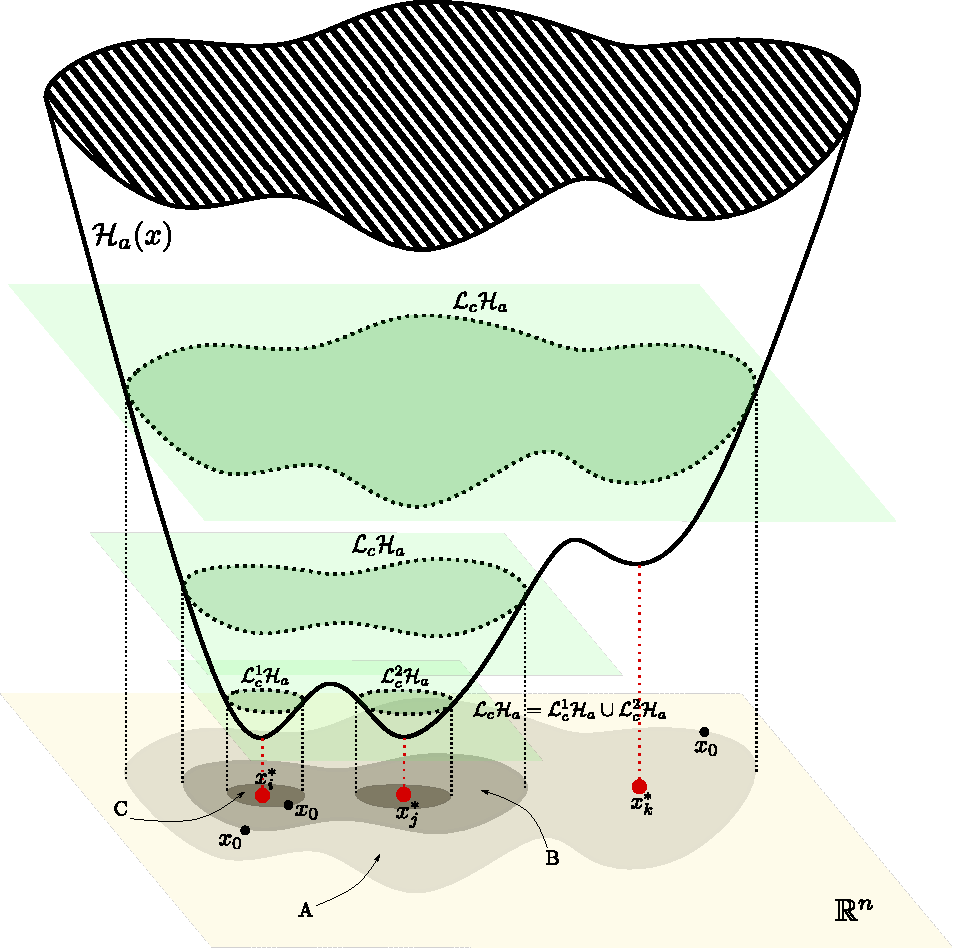
\includegraphics{draw2.pdf}
%	%% This file was created by matlab2tikz.
%
%The latest updates can be retrieved from
%  http://www.mathworks.com/matlabcentral/fileexchange/22022-matlab2tikz-matlab2tikz
%where you can also make suggestions and rate matlab2tikz.
%
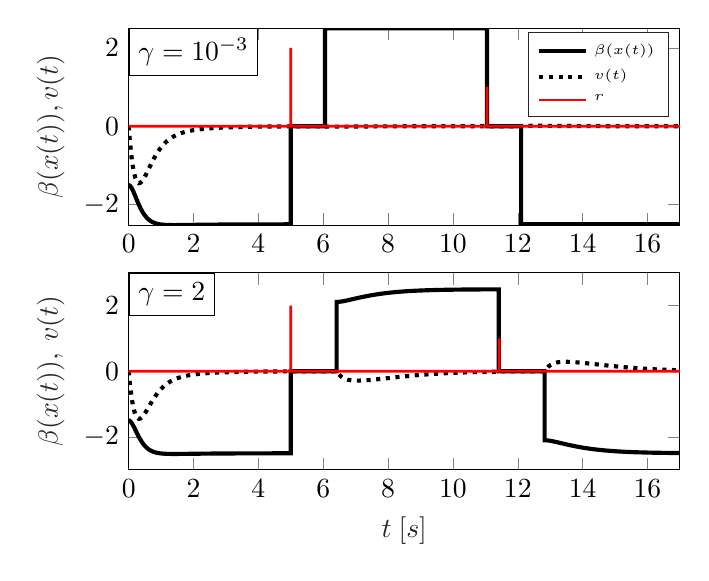
\begin{tikzpicture}

\begin{axis}[%
width=7cm,
height=2.5cm,
at={(0.758in,0.677in)},
scale only axis,
xmin=0,
xmax=17,
xlabel style={font=\color{white!15!black}},
xlabel={$t~[s]$},
ymin=-3,
ymax=3,
ylabel style={font=\color{white!15!black}},
ylabel={$\beta(x(t)),~v(t)$},
title = {${\gamma = 2}$},
every axis title/.style={below right,at={(0,1)},draw=black,fill=white},
axis background/.style={fill=white},
legend style={legend cell align=left, align=left, draw=white!15!black}
]
\addplot [color=black, line width=1.5pt]
  table[row sep=crcr]{%
0	-1.504\\
0.00201272951242755	-1.5040421239506\\
0.00402545902485509	-1.50416792485845\\
0.00603818853728264	-1.5043765408288\\
0.00805091804971019	-1.50466710296983\\
0.0181145656118479	-1.50731826395972\\
0.0281782131739857	-1.51188437125506\\
0.0382418607361234	-1.51825113419416\\
0.0483055082982611	-1.52630255249421\\
0.0872883339796663	-1.57124666864089\\
0.126271159661072	-1.63307936631001\\
0.165253985342477	-1.70570562615994\\
0.204236811023882	-1.78393666097299\\
0.258325242573133	-1.89406957792454\\
0.312413674122383	-1.99919533366988\\
0.366502105671634	-2.0946063144719\\
0.420590537220884	-2.17791827295709\\
0.481968041514646	-2.25709674809204\\
0.543345545808408	-2.3211017273968\\
0.60472305010217	-2.37177374143069\\
0.666100554395931	-2.41108279191348\\
0.724027870722878	-2.43960124498595\\
0.781955187049825	-2.46149216617405\\
0.839882503376772	-2.47812312445785\\
0.897809819703719	-2.49061320040479\\
0.966381939079961	-2.50129669674163\\
1.0349540584562	-2.50866455721899\\
1.10352617783245	-2.51361634287661\\
1.17209829720869	-2.51682148645407\\
1.24444068335681	-2.51885213351912\\
1.31678306950493	-2.51990312114615\\
1.38912545565305	-2.5202746069692\\
1.46146784180118	-2.52018130440801\\
1.5338102279493	-2.51977333101009\\
1.60615261409742	-2.51915819348171\\
1.67849500024554	-2.51841295850998\\
1.75083738639366	-2.51759034387962\\
1.83596904357362	-2.51657064140258\\
1.92110070075358	-2.51553710306555\\
2.00623235793354	-2.51451904955011\\
2.0913640151135	-2.51353114695333\\
2.18740015096789	-2.51246177380188\\
2.28343628682228	-2.51145317347952\\
2.37947242267667	-2.51051138378251\\
2.47550855853105	-2.50963427705357\\
2.58940334197328	-2.50867195136141\\
2.7032981254155	-2.50779651566838\\
2.81719290885772	-2.50700536225962\\
2.93108769229994	-2.50628926775151\\
3.05608769229994	-2.50557903978726\\
3.18108769229994	-2.50494582761179\\
3.30608769229994	-2.50438373443774\\
3.43108769229994	-2.5038835838969\\
3.55608769229994	-2.50343714479222\\
3.68108769229994	-2.50304104287402\\
3.80608769229994	-2.50269039482711\\
3.93108769229994	-2.50237953701534\\
4.05608769229994	-2.50210344689872\\
4.18108769229994	-2.5018590601567\\
4.30608769229994	-2.50164301703084\\
4.43108769229994	-2.50145185801545\\
4.55608769229994	-2.50128252248831\\
4.68108769229994	-2.50113282266486\\
4.80608769229994	-2.50100058926017\\
4.93108769229994	-2.50088371275499\\
4.94831576922496	-2.50086869645166\\
4.96554384614997	-2.50085393407084\\
4.98277192307499	-2.5008394213574\\
5	-2.50082515412478\\
5	0\\
5.001	0\\
5.002	0\\
5.003	0\\
5.004	0\\
5.005	0\\
5.006	0\\
5.007	0\\
5.008	0\\
5.009	0\\
5.01	0\\
5.011	0\\
5.012	0\\
5.013	0\\
5.014	0\\
5.015	0\\
5.016	0\\
5.017	0\\
5.018	0\\
5.019	0\\
5.02	0\\
5.021	0\\
5.022	0\\
5.023	0\\
5.024	0\\
5.025	0\\
5.026	0\\
5.027	0\\
5.028	0\\
5.029	0\\
5.03	0\\
5.031	0\\
5.032	0\\
5.033	0\\
5.034	0\\
5.035	0\\
5.036	0\\
5.037	0\\
5.038	0\\
5.039	0\\
5.04	0\\
5.041	0\\
5.042	0\\
5.043	0\\
5.044	0\\
5.045	0\\
5.046	0\\
5.047	0\\
5.048	0\\
5.049	0\\
5.05	0\\
5.051	0\\
5.052	0\\
5.053	0\\
5.054	0\\
5.055	0\\
5.056	0\\
5.057	0\\
5.058	0\\
5.059	0\\
5.06	0\\
5.061	0\\
5.062	0\\
5.063	0\\
5.064	0\\
5.065	0\\
5.066	0\\
5.067	0\\
5.068	0\\
5.069	0\\
5.07	0\\
5.071	0\\
5.072	0\\
5.073	0\\
5.074	0\\
5.075	0\\
5.076	0\\
5.077	0\\
5.078	0\\
5.079	0\\
5.08	0\\
5.081	0\\
5.082	0\\
5.083	0\\
5.084	0\\
5.085	0\\
5.086	0\\
5.087	0\\
5.088	0\\
5.089	0\\
5.09	0\\
5.091	0\\
5.092	0\\
5.093	0\\
5.094	0\\
5.095	0\\
5.096	0\\
5.097	0\\
5.098	0\\
5.099	0\\
5.1	0\\
5.101	0\\
5.102	0\\
5.103	0\\
5.104	0\\
5.105	0\\
5.106	0\\
5.107	0\\
5.108	0\\
5.109	0\\
5.11	0\\
5.111	0\\
5.112	0\\
5.113	0\\
5.114	0\\
5.115	0\\
5.116	0\\
5.117	0\\
5.118	0\\
5.119	0\\
5.12	0\\
5.121	0\\
5.122	0\\
5.123	0\\
5.124	0\\
5.125	0\\
5.126	0\\
5.127	0\\
5.128	0\\
5.129	0\\
5.13	0\\
5.131	0\\
5.132	0\\
5.133	0\\
5.134	0\\
5.135	0\\
5.136	0\\
5.137	0\\
5.138	0\\
5.139	0\\
5.14	0\\
5.141	0\\
5.142	0\\
5.143	0\\
5.144	0\\
5.145	0\\
5.146	0\\
5.147	0\\
5.148	0\\
5.149	0\\
5.15	0\\
5.151	0\\
5.152	0\\
5.153	0\\
5.154	0\\
5.155	0\\
5.156	0\\
5.157	0\\
5.158	0\\
5.159	0\\
5.16	0\\
5.161	0\\
5.162	0\\
5.163	0\\
5.164	0\\
5.165	0\\
5.166	0\\
5.167	0\\
5.168	0\\
5.169	0\\
5.17	0\\
5.171	0\\
5.172	0\\
5.173	0\\
5.174	0\\
5.175	0\\
5.176	0\\
5.177	0\\
5.178	0\\
5.179	0\\
5.18	0\\
5.181	0\\
5.182	0\\
5.183	0\\
5.184	0\\
5.185	0\\
5.186	0\\
5.187	0\\
5.188	0\\
5.189	0\\
5.19	0\\
5.191	0\\
5.192	0\\
5.193	0\\
5.194	0\\
5.195	0\\
5.196	0\\
5.197	0\\
5.198	0\\
5.199	0\\
5.2	0\\
5.201	0\\
5.202	0\\
5.203	0\\
5.204	0\\
5.205	0\\
5.206	0\\
5.207	0\\
5.208	0\\
5.209	0\\
5.21	0\\
5.211	0\\
5.212	0\\
5.213	0\\
5.214	0\\
5.215	0\\
5.216	0\\
5.217	0\\
5.218	0\\
5.219	0\\
5.22	0\\
5.221	0\\
5.222	0\\
5.223	0\\
5.224	0\\
5.225	0\\
5.226	0\\
5.227	0\\
5.228	0\\
5.229	0\\
5.23	0\\
5.231	0\\
5.232	0\\
5.233	0\\
5.234	0\\
5.235	0\\
5.236	0\\
5.237	0\\
5.238	0\\
5.239	0\\
5.24	0\\
5.241	0\\
5.242	0\\
5.243	0\\
5.244	0\\
5.245	0\\
5.246	0\\
5.247	0\\
5.248	0\\
5.249	0\\
5.25	0\\
5.251	0\\
5.252	0\\
5.253	0\\
5.254	0\\
5.255	0\\
5.256	0\\
5.257	0\\
5.258	0\\
5.259	0\\
5.26	0\\
5.261	0\\
5.262	0\\
5.263	0\\
5.264	0\\
5.265	0\\
5.266	0\\
5.267	0\\
5.268	0\\
5.269	0\\
5.27	0\\
5.271	0\\
5.272	0\\
5.273	0\\
5.274	0\\
5.275	0\\
5.276	0\\
5.277	0\\
5.278	0\\
5.279	0\\
5.28	0\\
5.281	0\\
5.282	0\\
5.283	0\\
5.284	0\\
5.285	0\\
5.286	0\\
5.287	0\\
5.288	0\\
5.289	0\\
5.29	0\\
5.291	0\\
5.292	0\\
5.293	0\\
5.294	0\\
5.295	0\\
5.296	0\\
5.297	0\\
5.298	0\\
5.299	0\\
5.3	0\\
5.301	0\\
5.302	0\\
5.303	0\\
5.304	0\\
5.305	0\\
5.306	0\\
5.307	0\\
5.308	0\\
5.309	0\\
5.31	0\\
5.311	0\\
5.312	0\\
5.313	0\\
5.314	0\\
5.315	0\\
5.316	0\\
5.317	0\\
5.318	0\\
5.319	0\\
5.32	0\\
5.321	0\\
5.322	0\\
5.323	0\\
5.324	0\\
5.325	0\\
5.326	0\\
5.327	0\\
5.328	0\\
5.329	0\\
5.33	0\\
5.331	0\\
5.332	0\\
5.333	0\\
5.334	0\\
5.335	0\\
5.336	0\\
5.337	0\\
5.338	0\\
5.339	0\\
5.34	0\\
5.341	0\\
5.342	0\\
5.343	0\\
5.344	0\\
5.345	0\\
5.346	0\\
5.347	0\\
5.348	0\\
5.349	0\\
5.35	0\\
5.351	0\\
5.352	0\\
5.353	0\\
5.354	0\\
5.355	0\\
5.356	0\\
5.357	0\\
5.358	0\\
5.359	0\\
5.36	0\\
5.361	0\\
5.362	0\\
5.363	0\\
5.364	0\\
5.365	0\\
5.366	0\\
5.367	0\\
5.368	0\\
5.369	0\\
5.37	0\\
5.371	0\\
5.372	0\\
5.373	0\\
5.374	0\\
5.375	0\\
5.376	0\\
5.377	0\\
5.378	0\\
5.379	0\\
5.38	0\\
5.381	0\\
5.382	0\\
5.383	0\\
5.384	0\\
5.385	0\\
5.386	0\\
5.387	0\\
5.388	0\\
5.389	0\\
5.39	0\\
5.391	0\\
5.392	0\\
5.393	0\\
5.394	0\\
5.395	0\\
5.396	0\\
5.397	0\\
5.398	0\\
5.399	0\\
5.4	0\\
5.401	0\\
5.402	0\\
5.403	0\\
5.404	0\\
5.405	0\\
5.406	0\\
5.407	0\\
5.408	0\\
5.409	0\\
5.41	0\\
5.411	0\\
5.412	0\\
5.413	0\\
5.414	0\\
5.415	0\\
5.416	0\\
5.417	0\\
5.418	0\\
5.419	0\\
5.42	0\\
5.421	0\\
5.422	0\\
5.423	0\\
5.424	0\\
5.425	0\\
5.426	0\\
5.427	0\\
5.428	0\\
5.429	0\\
5.43	0\\
5.431	0\\
5.432	0\\
5.433	0\\
5.434	0\\
5.435	0\\
5.436	0\\
5.437	0\\
5.438	0\\
5.439	0\\
5.44	0\\
5.441	0\\
5.442	0\\
5.443	0\\
5.444	0\\
5.445	0\\
5.446	0\\
5.447	0\\
5.448	0\\
5.449	0\\
5.45	0\\
5.451	0\\
5.452	0\\
5.453	0\\
5.454	0\\
5.455	0\\
5.456	0\\
5.457	0\\
5.458	0\\
5.459	0\\
5.46	0\\
5.461	0\\
5.462	0\\
5.463	0\\
5.464	0\\
5.465	0\\
5.466	0\\
5.467	0\\
5.468	0\\
5.469	0\\
5.47	0\\
5.471	0\\
5.472	0\\
5.473	0\\
5.474	0\\
5.475	0\\
5.476	0\\
5.477	0\\
5.478	0\\
5.479	0\\
5.48	0\\
5.481	0\\
5.482	0\\
5.483	0\\
5.484	0\\
5.485	0\\
5.486	0\\
5.487	0\\
5.488	0\\
5.489	0\\
5.49	0\\
5.491	0\\
5.492	0\\
5.493	0\\
5.494	0\\
5.495	0\\
5.496	0\\
5.497	0\\
5.498	0\\
5.499	0\\
5.5	0\\
5.501	0\\
5.502	0\\
5.503	0\\
5.504	0\\
5.505	0\\
5.506	0\\
5.507	0\\
5.508	0\\
5.509	0\\
5.51	0\\
5.511	0\\
5.512	0\\
5.513	0\\
5.514	0\\
5.515	0\\
5.516	0\\
5.517	0\\
5.518	0\\
5.519	0\\
5.52	0\\
5.521	0\\
5.522	0\\
5.523	0\\
5.524	0\\
5.525	0\\
5.526	0\\
5.527	0\\
5.528	0\\
5.529	0\\
5.53	0\\
5.531	0\\
5.532	0\\
5.533	0\\
5.534	0\\
5.535	0\\
5.536	0\\
5.537	0\\
5.538	0\\
5.539	0\\
5.54	0\\
5.541	0\\
5.542	0\\
5.543	0\\
5.544	0\\
5.545	0\\
5.546	0\\
5.547	0\\
5.548	0\\
5.549	0\\
5.55	0\\
5.551	0\\
5.552	0\\
5.553	0\\
5.554	0\\
5.555	0\\
5.556	0\\
5.557	0\\
5.558	0\\
5.559	0\\
5.56	0\\
5.561	0\\
5.562	0\\
5.563	0\\
5.564	0\\
5.565	0\\
5.566	0\\
5.567	0\\
5.568	0\\
5.569	0\\
5.57	0\\
5.571	0\\
5.572	0\\
5.573	0\\
5.574	0\\
5.575	0\\
5.576	0\\
5.577	0\\
5.578	0\\
5.579	0\\
5.58	0\\
5.581	0\\
5.582	0\\
5.583	0\\
5.584	0\\
5.585	0\\
5.586	0\\
5.587	0\\
5.588	0\\
5.589	0\\
5.59	0\\
5.591	0\\
5.592	0\\
5.593	0\\
5.594	0\\
5.595	0\\
5.596	0\\
5.597	0\\
5.598	0\\
5.599	0\\
5.6	0\\
5.601	0\\
5.602	0\\
5.603	0\\
5.604	0\\
5.605	0\\
5.606	0\\
5.607	0\\
5.608	0\\
5.609	0\\
5.61	0\\
5.611	0\\
5.612	0\\
5.613	0\\
5.614	0\\
5.615	0\\
5.616	0\\
5.617	0\\
5.618	0\\
5.619	0\\
5.62	0\\
5.621	0\\
5.622	0\\
5.623	0\\
5.624	0\\
5.625	0\\
5.626	0\\
5.627	0\\
5.628	0\\
5.629	0\\
5.63	0\\
5.631	0\\
5.632	0\\
5.633	0\\
5.634	0\\
5.635	0\\
5.636	0\\
5.637	0\\
5.638	0\\
5.639	0\\
5.64	0\\
5.641	0\\
5.642	0\\
5.643	0\\
5.644	0\\
5.645	0\\
5.646	0\\
5.647	0\\
5.648	0\\
5.649	0\\
5.65	0\\
5.651	0\\
5.652	0\\
5.653	0\\
5.654	0\\
5.655	0\\
5.656	0\\
5.657	0\\
5.658	0\\
5.659	0\\
5.66	0\\
5.661	0\\
5.662	0\\
5.663	0\\
5.664	0\\
5.665	0\\
5.666	0\\
5.667	0\\
5.668	0\\
5.669	0\\
5.67	0\\
5.671	0\\
5.672	0\\
5.673	0\\
5.674	0\\
5.675	0\\
5.676	0\\
5.677	0\\
5.678	0\\
5.679	0\\
5.68	0\\
5.681	0\\
5.682	0\\
5.683	0\\
5.684	0\\
5.685	0\\
5.686	0\\
5.687	0\\
5.688	0\\
5.689	0\\
5.69	0\\
5.691	0\\
5.692	0\\
5.693	0\\
5.694	0\\
5.695	0\\
5.696	0\\
5.697	0\\
5.698	0\\
5.699	0\\
5.7	0\\
5.701	0\\
5.702	0\\
5.703	0\\
5.704	0\\
5.705	0\\
5.706	0\\
5.707	0\\
5.708	0\\
5.709	0\\
5.71	0\\
5.711	0\\
5.712	0\\
5.713	0\\
5.714	0\\
5.715	0\\
5.716	0\\
5.717	0\\
5.718	0\\
5.719	0\\
5.72	0\\
5.721	0\\
5.722	0\\
5.723	0\\
5.724	0\\
5.725	0\\
5.726	0\\
5.727	0\\
5.728	0\\
5.729	0\\
5.73	0\\
5.731	0\\
5.732	0\\
5.733	0\\
5.734	0\\
5.735	0\\
5.736	0\\
5.737	0\\
5.738	0\\
5.739	0\\
5.74	0\\
5.741	0\\
5.742	0\\
5.743	0\\
5.744	0\\
5.745	0\\
5.746	0\\
5.747	0\\
5.748	0\\
5.749	0\\
5.75	0\\
5.751	0\\
5.752	0\\
5.753	0\\
5.754	0\\
5.755	0\\
5.756	0\\
5.757	0\\
5.758	0\\
5.759	0\\
5.76	0\\
5.761	0\\
5.762	0\\
5.763	0\\
5.764	0\\
5.765	0\\
5.766	0\\
5.767	0\\
5.768	0\\
5.769	0\\
5.77	0\\
5.771	0\\
5.772	0\\
5.773	0\\
5.774	0\\
5.775	0\\
5.776	0\\
5.777	0\\
5.778	0\\
5.779	0\\
5.78	0\\
5.781	0\\
5.782	0\\
5.783	0\\
5.784	0\\
5.785	0\\
5.786	0\\
5.787	0\\
5.788	0\\
5.789	0\\
5.79	0\\
5.791	0\\
5.792	0\\
5.793	0\\
5.794	0\\
5.795	0\\
5.796	0\\
5.797	0\\
5.798	0\\
5.799	0\\
5.8	0\\
5.801	0\\
5.802	0\\
5.803	0\\
5.804	0\\
5.805	0\\
5.806	0\\
5.807	0\\
5.808	0\\
5.809	0\\
5.81	0\\
5.811	0\\
5.812	0\\
5.813	0\\
5.814	0\\
5.815	0\\
5.816	0\\
5.817	0\\
5.818	0\\
5.819	0\\
5.82	0\\
5.821	0\\
5.822	0\\
5.823	0\\
5.824	0\\
5.825	0\\
5.826	0\\
5.827	0\\
5.828	0\\
5.829	0\\
5.83	0\\
5.831	0\\
5.832	0\\
5.833	0\\
5.834	0\\
5.835	0\\
5.836	0\\
5.837	0\\
5.838	0\\
5.839	0\\
5.84	0\\
5.841	0\\
5.842	0\\
5.843	0\\
5.844	0\\
5.845	0\\
5.846	0\\
5.847	0\\
5.848	0\\
5.849	0\\
5.85	0\\
5.851	0\\
5.852	0\\
5.853	0\\
5.854	0\\
5.855	0\\
5.856	0\\
5.857	0\\
5.858	0\\
5.859	0\\
5.86	0\\
5.861	0\\
5.862	0\\
5.863	0\\
5.864	0\\
5.865	0\\
5.866	0\\
5.867	0\\
5.868	0\\
5.869	0\\
5.87	0\\
5.871	0\\
5.872	0\\
5.873	0\\
5.874	0\\
5.875	0\\
5.876	0\\
5.877	0\\
5.878	0\\
5.879	0\\
5.88	0\\
5.881	0\\
5.882	0\\
5.883	0\\
5.884	0\\
5.885	0\\
5.886	0\\
5.887	0\\
5.888	0\\
5.889	0\\
5.89	0\\
5.891	0\\
5.892	0\\
5.893	0\\
5.894	0\\
5.895	0\\
5.896	0\\
5.897	0\\
5.898	0\\
5.899	0\\
5.9	0\\
5.901	0\\
5.902	0\\
5.903	0\\
5.904	0\\
5.905	0\\
5.906	0\\
5.907	0\\
5.908	0\\
5.909	0\\
5.91	0\\
5.911	0\\
5.912	0\\
5.913	0\\
5.914	0\\
5.915	0\\
5.916	0\\
5.917	0\\
5.918	0\\
5.919	0\\
5.92	0\\
5.921	0\\
5.922	0\\
5.923	0\\
5.924	0\\
5.925	0\\
5.926	0\\
5.927	0\\
5.928	0\\
5.929	0\\
5.93	0\\
5.931	0\\
5.932	0\\
5.933	0\\
5.934	0\\
5.935	0\\
5.936	0\\
5.937	0\\
5.938	0\\
5.939	0\\
5.94	0\\
5.941	0\\
5.942	0\\
5.943	0\\
5.944	0\\
5.945	0\\
5.946	0\\
5.947	0\\
5.948	0\\
5.949	0\\
5.95	0\\
5.951	0\\
5.952	0\\
5.953	0\\
5.954	0\\
5.955	0\\
5.956	0\\
5.957	0\\
5.958	0\\
5.959	0\\
5.96	0\\
5.961	0\\
5.962	0\\
5.963	0\\
5.964	0\\
5.965	0\\
5.966	0\\
5.967	0\\
5.968	0\\
5.969	0\\
5.97	0\\
5.971	0\\
5.972	0\\
5.973	0\\
5.974	0\\
5.975	0\\
5.976	0\\
5.977	0\\
5.978	0\\
5.979	0\\
5.98	0\\
5.981	0\\
5.982	0\\
5.983	0\\
5.984	0\\
5.985	0\\
5.986	0\\
5.987	0\\
5.988	0\\
5.989	0\\
5.99	0\\
5.991	0\\
5.992	0\\
5.993	0\\
5.994	0\\
5.995	0\\
5.996	0\\
5.997	0\\
5.998	0\\
5.999	0\\
6	0\\
6.001	0\\
6.002	0\\
6.003	0\\
6.004	0\\
6.005	0\\
6.006	0\\
6.007	0\\
6.008	0\\
6.009	0\\
6.01	0\\
6.011	0\\
6.012	0\\
6.013	0\\
6.014	0\\
6.015	0\\
6.016	0\\
6.017	0\\
6.018	0\\
6.019	0\\
6.02	0\\
6.021	0\\
6.022	0\\
6.023	0\\
6.024	0\\
6.025	0\\
6.026	0\\
6.027	0\\
6.028	0\\
6.029	0\\
6.03	0\\
6.031	0\\
6.032	0\\
6.033	0\\
6.034	0\\
6.035	0\\
6.036	0\\
6.037	0\\
6.038	0\\
6.039	0\\
6.04	0\\
6.041	0\\
6.042	0\\
6.043	0\\
6.044	0\\
6.045	0\\
6.046	0\\
6.047	0\\
6.048	0\\
6.049	0\\
6.05	0\\
6.051	0\\
6.052	0\\
6.053	0\\
6.054	0\\
6.055	0\\
6.056	0\\
6.057	0\\
6.058	0\\
6.059	0\\
6.06	0\\
6.061	0\\
6.062	0\\
6.063	0\\
6.064	0\\
6.065	0\\
6.066	0\\
6.067	0\\
6.068	0\\
6.069	0\\
6.07	0\\
6.071	0\\
6.072	0\\
6.073	0\\
6.074	0\\
6.075	0\\
6.076	0\\
6.077	0\\
6.078	0\\
6.079	0\\
6.08	0\\
6.081	0\\
6.082	0\\
6.083	0\\
6.084	0\\
6.085	0\\
6.086	0\\
6.087	0\\
6.088	0\\
6.089	0\\
6.09	0\\
6.091	0\\
6.092	0\\
6.093	0\\
6.094	0\\
6.095	0\\
6.096	0\\
6.097	0\\
6.098	0\\
6.099	0\\
6.1	0\\
6.101	0\\
6.102	0\\
6.103	0\\
6.104	0\\
6.105	0\\
6.106	0\\
6.107	0\\
6.108	0\\
6.109	0\\
6.11	0\\
6.111	0\\
6.112	0\\
6.113	0\\
6.114	0\\
6.115	0\\
6.116	0\\
6.117	0\\
6.118	0\\
6.119	0\\
6.12	0\\
6.121	0\\
6.122	0\\
6.123	0\\
6.124	0\\
6.125	0\\
6.126	0\\
6.127	0\\
6.128	0\\
6.129	0\\
6.13	0\\
6.131	0\\
6.132	0\\
6.133	0\\
6.134	0\\
6.135	0\\
6.136	0\\
6.137	0\\
6.138	0\\
6.139	0\\
6.14	0\\
6.141	0\\
6.142	0\\
6.143	0\\
6.144	0\\
6.145	0\\
6.146	0\\
6.147	0\\
6.148	0\\
6.149	0\\
6.15	0\\
6.151	0\\
6.152	0\\
6.153	0\\
6.154	0\\
6.155	0\\
6.156	0\\
6.157	0\\
6.158	0\\
6.159	0\\
6.16	0\\
6.161	0\\
6.162	0\\
6.163	0\\
6.164	0\\
6.165	0\\
6.166	0\\
6.167	0\\
6.168	0\\
6.169	0\\
6.17	0\\
6.171	0\\
6.172	0\\
6.173	0\\
6.174	0\\
6.175	0\\
6.176	0\\
6.177	0\\
6.178	0\\
6.179	0\\
6.18	0\\
6.181	0\\
6.182	0\\
6.183	0\\
6.184	0\\
6.185	0\\
6.186	0\\
6.187	0\\
6.188	0\\
6.189	0\\
6.19	0\\
6.191	0\\
6.192	0\\
6.193	0\\
6.194	0\\
6.195	0\\
6.196	0\\
6.197	0\\
6.198	0\\
6.199	0\\
6.2	0\\
6.201	0\\
6.202	0\\
6.203	0\\
6.204	0\\
6.205	0\\
6.206	0\\
6.207	0\\
6.208	0\\
6.209	0\\
6.21	0\\
6.211	0\\
6.212	0\\
6.213	0\\
6.214	0\\
6.215	0\\
6.216	0\\
6.217	0\\
6.218	0\\
6.219	0\\
6.22	0\\
6.221	0\\
6.222	0\\
6.223	0\\
6.224	0\\
6.225	0\\
6.226	0\\
6.227	0\\
6.228	0\\
6.229	0\\
6.23	0\\
6.231	0\\
6.232	0\\
6.233	0\\
6.234	0\\
6.235	0\\
6.236	0\\
6.237	0\\
6.238	0\\
6.239	0\\
6.24	0\\
6.241	0\\
6.242	0\\
6.243	0\\
6.244	0\\
6.245	0\\
6.246	0\\
6.247	0\\
6.248	0\\
6.249	0\\
6.25	0\\
6.251	0\\
6.252	0\\
6.253	0\\
6.254	0\\
6.255	0\\
6.256	0\\
6.257	0\\
6.258	0\\
6.259	0\\
6.26	0\\
6.261	0\\
6.262	0\\
6.263	0\\
6.264	0\\
6.265	0\\
6.266	0\\
6.267	0\\
6.268	0\\
6.269	0\\
6.27	0\\
6.271	0\\
6.272	0\\
6.273	0\\
6.274	0\\
6.275	0\\
6.276	0\\
6.277	0\\
6.278	0\\
6.279	0\\
6.28	0\\
6.281	0\\
6.282	0\\
6.283	0\\
6.284	0\\
6.285	0\\
6.286	0\\
6.287	0\\
6.288	0\\
6.289	0\\
6.29	0\\
6.291	0\\
6.292	0\\
6.293	0\\
6.294	0\\
6.295	0\\
6.296	0\\
6.297	0\\
6.298	0\\
6.299	0\\
6.3	0\\
6.301	0\\
6.302	0\\
6.303	0\\
6.304	0\\
6.305	0\\
6.306	0\\
6.307	0\\
6.308	0\\
6.309	0\\
6.31	0\\
6.311	0\\
6.312	0\\
6.313	0\\
6.314	0\\
6.315	0\\
6.316	0\\
6.317	0\\
6.318	0\\
6.319	0\\
6.32	0\\
6.321	0\\
6.322	0\\
6.323	0\\
6.324	0\\
6.325	0\\
6.326	0\\
6.327	0\\
6.328	0\\
6.329	0\\
6.33	0\\
6.331	0\\
6.332	0\\
6.333	0\\
6.334	0\\
6.335	0\\
6.336	0\\
6.337	0\\
6.338	0\\
6.339	0\\
6.34	0\\
6.341	0\\
6.342	0\\
6.343	0\\
6.344	0\\
6.345	0\\
6.346	0\\
6.347	0\\
6.348	0\\
6.349	0\\
6.35	0\\
6.351	0\\
6.352	0\\
6.353	0\\
6.354	0\\
6.355	0\\
6.356	0\\
6.357	0\\
6.358	0\\
6.359	0\\
6.36	0\\
6.361	0\\
6.362	0\\
6.363	0\\
6.364	0\\
6.365	0\\
6.366	0\\
6.367	0\\
6.368	0\\
6.369	0\\
6.37	0\\
6.371	0\\
6.372	0\\
6.373	0\\
6.374	0\\
6.375	0\\
6.376	0\\
6.377	0\\
6.378	0\\
6.379	0\\
6.38	0\\
6.381	0\\
6.382	0\\
6.383	0\\
6.384	0\\
6.385	0\\
6.386	0\\
6.387	0\\
6.388	0\\
6.389	0\\
6.39	0\\
6.391	0\\
6.392	0\\
6.393	0\\
6.394	0\\
6.395	0\\
6.396	0\\
6.397	0\\
6.398	0\\
6.399	0\\
6.4	0\\
6.401	0\\
6.402	0\\
6.403	0\\
6.404	0\\
6.405	0\\
6.406	0\\
6.407	0\\
6.408	0\\
6.409	0\\
6.41	0\\
6.411	0\\
6.412	0\\
6.413	0\\
6.413	2.1139316693639\\
6.42730885570975	2.11412234770866\\
6.44161771141949	2.11458271024684\\
6.45592656712924	2.11529371448898\\
6.47023542283898	2.11623730139078\\
6.51517744734551	2.12051536201303\\
6.56011947185204	2.12647179532107\\
6.60506149635856	2.13374199061386\\
6.65000352086509	2.14199088166887\\
6.69559714700642	2.15108018188364\\
6.74119077314774	2.16071170234008\\
6.78678439928907	2.17072203975994\\
6.8323780254304	2.18096387958857\\
6.88670805540013	2.19330626627053\\
6.94103808536987	2.20568431358523\\
6.99536811533961	2.21799547886423\\
7.04969814530934	2.23014459971016\\
7.11365261721454	2.24413990213848\\
7.17760708911974	2.25775481596045\\
7.24156156102494	2.27094416057966\\
7.30551603293014	2.28366181904244\\
7.38197671782709	2.29820259589554\\
7.45843740272405	2.31202215669435\\
7.53489808762101	2.32512097853371\\
7.61135877251796	2.33749059854897\\
7.70134213864231	2.35111319564808\\
7.79132550476665	2.36377548890919\\
7.881308870891	2.37552126397596\\
7.97129223701534	2.38637583335275\\
8.0720438339047	2.39750761836149\\
8.17279543079405	2.40764965442173\\
8.2735470276834	2.41687774399794\\
8.37429862457275	2.42524102782635\\
8.48225357766335	2.43329893616551\\
8.59020853075395	2.4405259071389\\
8.69816348384455	2.44700551552019\\
8.80611843693515	2.45279324233867\\
8.92128733479583	2.45826485434564\\
9.03645623265651	2.46310783902498\\
9.15162513051719	2.46739810847239\\
9.26679402837787	2.47118562009055\\
9.39145950708824	2.47477211193423\\
9.5161249857986	2.47790727384046\\
9.64079046450896	2.48065387234801\\
9.76545594321933	2.48305175466436\\
9.89045594321933	2.48514257981024\\
10.0154559432193	2.48697055340701\\
10.1404559432193	2.48857224898578\\
10.2654559432193	2.48997245973096\\
10.3904559432193	2.49119341101114\\
10.5154559432193	2.49226286926307\\
10.6404559432193	2.49320134333166\\
10.7654559432193	2.49402372946499\\
10.8904559432193	2.49474323306017\\
11.0154559432193	2.49537478040974\\
11.1404559432193	2.49592985873586\\
11.2654559432193	2.49641733974889\\
11.3023419574145	2.49654937647319\\
11.3392279716097	2.49667648026421\\
11.3761139858048	2.49679883926087\\
11.413	2.49691663406204\\
11.413	0\\
11.414	0\\
11.415	0\\
11.416	0\\
11.417	0\\
11.418	0\\
11.419	0\\
11.42	0\\
11.421	0\\
11.422	0\\
11.423	0\\
11.424	0\\
11.425	0\\
11.426	0\\
11.427	0\\
11.428	0\\
11.429	0\\
11.43	0\\
11.431	0\\
11.432	0\\
11.433	0\\
11.434	0\\
11.435	0\\
11.436	0\\
11.437	0\\
11.438	0\\
11.439	0\\
11.44	0\\
11.441	0\\
11.442	0\\
11.443	0\\
11.444	0\\
11.445	0\\
11.446	0\\
11.447	0\\
11.448	0\\
11.449	0\\
11.45	0\\
11.451	0\\
11.452	0\\
11.453	0\\
11.454	0\\
11.455	0\\
11.456	0\\
11.457	0\\
11.458	0\\
11.459	0\\
11.46	0\\
11.461	0\\
11.462	0\\
11.463	0\\
11.464	0\\
11.465	0\\
11.466	0\\
11.467	0\\
11.468	0\\
11.469	0\\
11.47	0\\
11.471	0\\
11.472	0\\
11.473	0\\
11.474	0\\
11.475	0\\
11.476	0\\
11.477	0\\
11.478	0\\
11.479	0\\
11.48	0\\
11.481	0\\
11.482	0\\
11.483	0\\
11.484	0\\
11.485	0\\
11.486	0\\
11.487	0\\
11.488	0\\
11.489	0\\
11.49	0\\
11.491	0\\
11.492	0\\
11.493	0\\
11.494	0\\
11.495	0\\
11.496	0\\
11.497	0\\
11.498	0\\
11.499	0\\
11.5	0\\
11.501	0\\
11.502	0\\
11.503	0\\
11.504	0\\
11.505	0\\
11.506	0\\
11.507	0\\
11.508	0\\
11.509	0\\
11.51	0\\
11.511	0\\
11.512	0\\
11.513	0\\
11.514	0\\
11.515	0\\
11.516	0\\
11.517	0\\
11.518	0\\
11.519	0\\
11.52	0\\
11.521	0\\
11.522	0\\
11.523	0\\
11.524	0\\
11.525	0\\
11.526	0\\
11.527	0\\
11.528	0\\
11.529	0\\
11.53	0\\
11.531	0\\
11.532	0\\
11.533	0\\
11.534	0\\
11.535	0\\
11.536	0\\
11.537	0\\
11.538	0\\
11.539	0\\
11.54	0\\
11.541	0\\
11.542	0\\
11.543	0\\
11.544	0\\
11.545	0\\
11.546	0\\
11.547	0\\
11.548	0\\
11.549	0\\
11.55	0\\
11.551	0\\
11.552	0\\
11.553	0\\
11.554	0\\
11.555	0\\
11.556	0\\
11.557	0\\
11.558	0\\
11.559	0\\
11.56	0\\
11.561	0\\
11.562	0\\
11.563	0\\
11.564	0\\
11.565	0\\
11.566	0\\
11.567	0\\
11.568	0\\
11.569	0\\
11.57	0\\
11.571	0\\
11.572	0\\
11.573	0\\
11.574	0\\
11.575	0\\
11.576	0\\
11.577	0\\
11.578	0\\
11.579	0\\
11.58	0\\
11.581	0\\
11.582	0\\
11.583	0\\
11.584	0\\
11.585	0\\
11.586	0\\
11.587	0\\
11.588	0\\
11.589	0\\
11.59	0\\
11.591	0\\
11.592	0\\
11.593	0\\
11.594	0\\
11.595	0\\
11.596	0\\
11.597	0\\
11.598	0\\
11.599	0\\
11.6	0\\
11.601	0\\
11.602	0\\
11.603	0\\
11.604	0\\
11.605	0\\
11.606	0\\
11.607	0\\
11.608	0\\
11.609	0\\
11.61	0\\
11.611	0\\
11.612	0\\
11.613	0\\
11.614	0\\
11.615	0\\
11.616	0\\
11.617	0\\
11.618	0\\
11.619	0\\
11.62	0\\
11.621	0\\
11.622	0\\
11.623	0\\
11.624	0\\
11.625	0\\
11.626	0\\
11.627	0\\
11.628	0\\
11.629	0\\
11.63	0\\
11.631	0\\
11.632	0\\
11.633	0\\
11.634	0\\
11.635	0\\
11.636	0\\
11.637	0\\
11.638	0\\
11.639	0\\
11.64	0\\
11.641	0\\
11.642	0\\
11.643	0\\
11.644	0\\
11.645	0\\
11.646	0\\
11.647	0\\
11.648	0\\
11.649	0\\
11.65	0\\
11.651	0\\
11.652	0\\
11.653	0\\
11.654	0\\
11.655	0\\
11.656	0\\
11.657	0\\
11.658	0\\
11.659	0\\
11.66	0\\
11.661	0\\
11.662	0\\
11.663	0\\
11.664	0\\
11.665	0\\
11.666	0\\
11.667	0\\
11.668	0\\
11.669	0\\
11.67	0\\
11.671	0\\
11.672	0\\
11.673	0\\
11.674	0\\
11.675	0\\
11.676	0\\
11.677	0\\
11.678	0\\
11.679	0\\
11.68	0\\
11.681	0\\
11.682	0\\
11.683	0\\
11.684	0\\
11.685	0\\
11.686	0\\
11.687	0\\
11.688	0\\
11.689	0\\
11.69	0\\
11.691	0\\
11.692	0\\
11.693	0\\
11.694	0\\
11.695	0\\
11.696	0\\
11.697	0\\
11.698	0\\
11.699	0\\
11.7	0\\
11.701	0\\
11.702	0\\
11.703	0\\
11.704	0\\
11.705	0\\
11.706	0\\
11.707	0\\
11.708	0\\
11.709	0\\
11.71	0\\
11.711	0\\
11.712	0\\
11.713	0\\
11.714	0\\
11.715	0\\
11.716	0\\
11.717	0\\
11.718	0\\
11.719	0\\
11.72	0\\
11.721	0\\
11.722	0\\
11.723	0\\
11.724	0\\
11.725	0\\
11.726	0\\
11.727	0\\
11.728	0\\
11.729	0\\
11.73	0\\
11.731	0\\
11.732	0\\
11.733	0\\
11.734	0\\
11.735	0\\
11.736	0\\
11.737	0\\
11.738	0\\
11.739	0\\
11.74	0\\
11.741	0\\
11.742	0\\
11.743	0\\
11.744	0\\
11.745	0\\
11.746	0\\
11.747	0\\
11.748	0\\
11.749	0\\
11.75	0\\
11.751	0\\
11.752	0\\
11.753	0\\
11.754	0\\
11.755	0\\
11.756	0\\
11.757	0\\
11.758	0\\
11.759	0\\
11.76	0\\
11.761	0\\
11.762	0\\
11.763	0\\
11.764	0\\
11.765	0\\
11.766	0\\
11.767	0\\
11.768	0\\
11.769	0\\
11.77	0\\
11.771	0\\
11.772	0\\
11.773	0\\
11.774	0\\
11.775	0\\
11.776	0\\
11.777	0\\
11.778	0\\
11.779	0\\
11.78	0\\
11.781	0\\
11.782	0\\
11.783	0\\
11.784	0\\
11.785	0\\
11.786	0\\
11.787	0\\
11.788	0\\
11.789	0\\
11.79	0\\
11.791	0\\
11.792	0\\
11.793	0\\
11.794	0\\
11.795	0\\
11.796	0\\
11.797	0\\
11.798	0\\
11.799	0\\
11.8	0\\
11.801	0\\
11.802	0\\
11.803	0\\
11.804	0\\
11.805	0\\
11.806	0\\
11.807	0\\
11.808	0\\
11.809	0\\
11.81	0\\
11.811	0\\
11.812	0\\
11.813	0\\
11.814	0\\
11.815	0\\
11.816	0\\
11.817	0\\
11.818	0\\
11.819	0\\
11.82	0\\
11.821	0\\
11.822	0\\
11.823	0\\
11.824	0\\
11.825	0\\
11.826	0\\
11.827	0\\
11.828	0\\
11.829	0\\
11.83	0\\
11.831	0\\
11.832	0\\
11.833	0\\
11.834	0\\
11.835	0\\
11.836	0\\
11.837	0\\
11.838	0\\
11.839	0\\
11.84	0\\
11.841	0\\
11.842	0\\
11.843	0\\
11.844	0\\
11.845	0\\
11.846	0\\
11.847	0\\
11.848	0\\
11.849	0\\
11.85	0\\
11.851	0\\
11.852	0\\
11.853	0\\
11.854	0\\
11.855	0\\
11.856	0\\
11.857	0\\
11.858	0\\
11.859	0\\
11.86	0\\
11.861	0\\
11.862	0\\
11.863	0\\
11.864	0\\
11.865	0\\
11.866	0\\
11.867	0\\
11.868	0\\
11.869	0\\
11.87	0\\
11.871	0\\
11.872	0\\
11.873	0\\
11.874	0\\
11.875	0\\
11.876	0\\
11.877	0\\
11.878	0\\
11.879	0\\
11.88	0\\
11.881	0\\
11.882	0\\
11.883	0\\
11.884	0\\
11.885	0\\
11.886	0\\
11.887	0\\
11.888	0\\
11.889	0\\
11.89	0\\
11.891	0\\
11.892	0\\
11.893	0\\
11.894	0\\
11.895	0\\
11.896	0\\
11.897	0\\
11.898	0\\
11.899	0\\
11.9	0\\
11.901	0\\
11.902	0\\
11.903	0\\
11.904	0\\
11.905	0\\
11.906	0\\
11.907	0\\
11.908	0\\
11.909	0\\
11.91	0\\
11.911	0\\
11.912	0\\
11.913	0\\
11.914	0\\
11.915	0\\
11.916	0\\
11.917	0\\
11.918	0\\
11.919	0\\
11.92	0\\
11.921	0\\
11.922	0\\
11.923	0\\
11.924	0\\
11.925	0\\
11.926	0\\
11.927	0\\
11.928	0\\
11.929	0\\
11.93	0\\
11.931	0\\
11.932	0\\
11.933	0\\
11.934	0\\
11.935	0\\
11.936	0\\
11.937	0\\
11.938	0\\
11.939	0\\
11.94	0\\
11.941	0\\
11.942	0\\
11.943	0\\
11.944	0\\
11.945	0\\
11.946	0\\
11.947	0\\
11.948	0\\
11.949	0\\
11.95	0\\
11.951	0\\
11.952	0\\
11.953	0\\
11.954	0\\
11.955	0\\
11.956	0\\
11.957	0\\
11.958	0\\
11.959	0\\
11.96	0\\
11.961	0\\
11.962	0\\
11.963	0\\
11.964	0\\
11.965	0\\
11.966	0\\
11.967	0\\
11.968	0\\
11.969	0\\
11.97	0\\
11.971	0\\
11.972	0\\
11.973	0\\
11.974	0\\
11.975	0\\
11.976	0\\
11.977	0\\
11.978	0\\
11.979	0\\
11.98	0\\
11.981	0\\
11.982	0\\
11.983	0\\
11.984	0\\
11.985	0\\
11.986	0\\
11.987	0\\
11.988	0\\
11.989	0\\
11.99	0\\
11.991	0\\
11.992	0\\
11.993	0\\
11.994	0\\
11.995	0\\
11.996	0\\
11.997	0\\
11.998	0\\
11.999	0\\
12	0\\
12.001	0\\
12.002	0\\
12.003	0\\
12.004	0\\
12.005	0\\
12.006	0\\
12.007	0\\
12.008	0\\
12.009	0\\
12.01	0\\
12.011	0\\
12.012	0\\
12.013	0\\
12.014	0\\
12.015	0\\
12.016	0\\
12.017	0\\
12.018	0\\
12.019	0\\
12.02	0\\
12.021	0\\
12.022	0\\
12.023	0\\
12.024	0\\
12.025	0\\
12.026	0\\
12.027	0\\
12.028	0\\
12.029	0\\
12.03	0\\
12.031	0\\
12.032	0\\
12.033	0\\
12.034	0\\
12.035	0\\
12.036	0\\
12.037	0\\
12.038	0\\
12.039	0\\
12.04	0\\
12.041	0\\
12.042	0\\
12.043	0\\
12.044	0\\
12.045	0\\
12.046	0\\
12.047	0\\
12.048	0\\
12.049	0\\
12.05	0\\
12.051	0\\
12.052	0\\
12.053	0\\
12.054	0\\
12.055	0\\
12.056	0\\
12.057	0\\
12.058	0\\
12.059	0\\
12.06	0\\
12.061	0\\
12.062	0\\
12.063	0\\
12.064	0\\
12.065	0\\
12.066	0\\
12.067	0\\
12.068	0\\
12.069	0\\
12.07	0\\
12.071	0\\
12.072	0\\
12.073	0\\
12.074	0\\
12.075	0\\
12.076	0\\
12.077	0\\
12.078	0\\
12.079	0\\
12.08	0\\
12.081	0\\
12.082	0\\
12.083	0\\
12.084	0\\
12.085	0\\
12.086	0\\
12.087	0\\
12.088	0\\
12.089	0\\
12.09	0\\
12.091	0\\
12.092	0\\
12.093	0\\
12.094	0\\
12.095	0\\
12.096	0\\
12.097	0\\
12.098	0\\
12.099	0\\
12.1	0\\
12.101	0\\
12.102	0\\
12.103	0\\
12.104	0\\
12.105	0\\
12.106	0\\
12.107	0\\
12.108	0\\
12.109	0\\
12.11	0\\
12.111	0\\
12.112	0\\
12.113	0\\
12.114	0\\
12.115	0\\
12.116	0\\
12.117	0\\
12.118	0\\
12.119	0\\
12.12	0\\
12.121	0\\
12.122	0\\
12.123	0\\
12.124	0\\
12.125	0\\
12.126	0\\
12.127	0\\
12.128	0\\
12.129	0\\
12.13	0\\
12.131	0\\
12.132	0\\
12.133	0\\
12.134	0\\
12.135	0\\
12.136	0\\
12.137	0\\
12.138	0\\
12.139	0\\
12.14	0\\
12.141	0\\
12.142	0\\
12.143	0\\
12.144	0\\
12.145	0\\
12.146	0\\
12.147	0\\
12.148	0\\
12.149	0\\
12.15	0\\
12.151	0\\
12.152	0\\
12.153	0\\
12.154	0\\
12.155	0\\
12.156	0\\
12.157	0\\
12.158	0\\
12.159	0\\
12.16	0\\
12.161	0\\
12.162	0\\
12.163	0\\
12.164	0\\
12.165	0\\
12.166	0\\
12.167	0\\
12.168	0\\
12.169	0\\
12.17	0\\
12.171	0\\
12.172	0\\
12.173	0\\
12.174	0\\
12.175	0\\
12.176	0\\
12.177	0\\
12.178	0\\
12.179	0\\
12.18	0\\
12.181	0\\
12.182	0\\
12.183	0\\
12.184	0\\
12.185	0\\
12.186	0\\
12.187	0\\
12.188	0\\
12.189	0\\
12.19	0\\
12.191	0\\
12.192	0\\
12.193	0\\
12.194	0\\
12.195	0\\
12.196	0\\
12.197	0\\
12.198	0\\
12.199	0\\
12.2	0\\
12.201	0\\
12.202	0\\
12.203	0\\
12.204	0\\
12.205	0\\
12.206	0\\
12.207	0\\
12.208	0\\
12.209	0\\
12.21	0\\
12.211	0\\
12.212	0\\
12.213	0\\
12.214	0\\
12.215	0\\
12.216	0\\
12.217	0\\
12.218	0\\
12.219	0\\
12.22	0\\
12.221	0\\
12.222	0\\
12.223	0\\
12.224	0\\
12.225	0\\
12.226	0\\
12.227	0\\
12.228	0\\
12.229	0\\
12.23	0\\
12.231	0\\
12.232	0\\
12.233	0\\
12.234	0\\
12.235	0\\
12.236	0\\
12.237	0\\
12.238	0\\
12.239	0\\
12.24	0\\
12.241	0\\
12.242	0\\
12.243	0\\
12.244	0\\
12.245	0\\
12.246	0\\
12.247	0\\
12.248	0\\
12.249	0\\
12.25	0\\
12.251	0\\
12.252	0\\
12.253	0\\
12.254	0\\
12.255	0\\
12.256	0\\
12.257	0\\
12.258	0\\
12.259	0\\
12.26	0\\
12.261	0\\
12.262	0\\
12.263	0\\
12.264	0\\
12.265	0\\
12.266	0\\
12.267	0\\
12.268	0\\
12.269	0\\
12.27	0\\
12.271	0\\
12.272	0\\
12.273	0\\
12.274	0\\
12.275	0\\
12.276	0\\
12.277	0\\
12.278	0\\
12.279	0\\
12.28	0\\
12.281	0\\
12.282	0\\
12.283	0\\
12.284	0\\
12.285	0\\
12.286	0\\
12.287	0\\
12.288	0\\
12.289	0\\
12.29	0\\
12.291	0\\
12.292	0\\
12.293	0\\
12.294	0\\
12.295	0\\
12.296	0\\
12.297	0\\
12.298	0\\
12.299	0\\
12.3	0\\
12.301	0\\
12.302	0\\
12.303	0\\
12.304	0\\
12.305	0\\
12.306	0\\
12.307	0\\
12.308	0\\
12.309	0\\
12.31	0\\
12.311	0\\
12.312	0\\
12.313	0\\
12.314	0\\
12.315	0\\
12.316	0\\
12.317	0\\
12.318	0\\
12.319	0\\
12.32	0\\
12.321	0\\
12.322	0\\
12.323	0\\
12.324	0\\
12.325	0\\
12.326	0\\
12.327	0\\
12.328	0\\
12.329	0\\
12.33	0\\
12.331	0\\
12.332	0\\
12.333	0\\
12.334	0\\
12.335	0\\
12.336	0\\
12.337	0\\
12.338	0\\
12.339	0\\
12.34	0\\
12.341	0\\
12.342	0\\
12.343	0\\
12.344	0\\
12.345	0\\
12.346	0\\
12.347	0\\
12.348	0\\
12.349	0\\
12.35	0\\
12.351	0\\
12.352	0\\
12.353	0\\
12.354	0\\
12.355	0\\
12.356	0\\
12.357	0\\
12.358	0\\
12.359	0\\
12.36	0\\
12.361	0\\
12.362	0\\
12.363	0\\
12.364	0\\
12.365	0\\
12.366	0\\
12.367	0\\
12.368	0\\
12.369	0\\
12.37	0\\
12.371	0\\
12.372	0\\
12.373	0\\
12.374	0\\
12.375	0\\
12.376	0\\
12.377	0\\
12.378	0\\
12.379	0\\
12.38	0\\
12.381	0\\
12.382	0\\
12.383	0\\
12.384	0\\
12.385	0\\
12.386	0\\
12.387	0\\
12.388	0\\
12.389	0\\
12.39	0\\
12.391	0\\
12.392	0\\
12.393	0\\
12.394	0\\
12.395	0\\
12.396	0\\
12.397	0\\
12.398	0\\
12.399	0\\
12.4	0\\
12.401	0\\
12.402	0\\
12.403	0\\
12.404	0\\
12.405	0\\
12.406	0\\
12.407	0\\
12.408	0\\
12.409	0\\
12.41	0\\
12.411	0\\
12.412	0\\
12.413	0\\
12.414	0\\
12.415	0\\
12.416	0\\
12.417	0\\
12.418	0\\
12.419	0\\
12.42	0\\
12.421	0\\
12.422	0\\
12.423	0\\
12.424	0\\
12.425	0\\
12.426	0\\
12.427	0\\
12.428	0\\
12.429	0\\
12.43	0\\
12.431	0\\
12.432	0\\
12.433	0\\
12.434	0\\
12.435	0\\
12.436	0\\
12.437	0\\
12.438	0\\
12.439	0\\
12.44	0\\
12.441	0\\
12.442	0\\
12.443	0\\
12.444	0\\
12.445	0\\
12.446	0\\
12.447	0\\
12.448	0\\
12.449	0\\
12.45	0\\
12.451	0\\
12.452	0\\
12.453	0\\
12.454	0\\
12.455	0\\
12.456	0\\
12.457	0\\
12.458	0\\
12.459	0\\
12.46	0\\
12.461	0\\
12.462	0\\
12.463	0\\
12.464	0\\
12.465	0\\
12.466	0\\
12.467	0\\
12.468	0\\
12.469	0\\
12.47	0\\
12.471	0\\
12.472	0\\
12.473	0\\
12.474	0\\
12.475	0\\
12.476	0\\
12.477	0\\
12.478	0\\
12.479	0\\
12.48	0\\
12.481	0\\
12.482	0\\
12.483	0\\
12.484	0\\
12.485	0\\
12.486	0\\
12.487	0\\
12.488	0\\
12.489	0\\
12.49	0\\
12.491	0\\
12.492	0\\
12.493	0\\
12.494	0\\
12.495	0\\
12.496	0\\
12.497	0\\
12.498	0\\
12.499	0\\
12.5	0\\
12.501	0\\
12.502	0\\
12.503	0\\
12.504	0\\
12.505	0\\
12.506	0\\
12.507	0\\
12.508	0\\
12.509	0\\
12.51	0\\
12.511	0\\
12.512	0\\
12.513	0\\
12.514	0\\
12.515	0\\
12.516	0\\
12.517	0\\
12.518	0\\
12.519	0\\
12.52	0\\
12.521	0\\
12.522	0\\
12.523	0\\
12.524	0\\
12.525	0\\
12.526	0\\
12.527	0\\
12.528	0\\
12.529	0\\
12.53	0\\
12.531	0\\
12.532	0\\
12.533	0\\
12.534	0\\
12.535	0\\
12.536	0\\
12.537	0\\
12.538	0\\
12.539	0\\
12.54	0\\
12.541	0\\
12.542	0\\
12.543	0\\
12.544	0\\
12.545	0\\
12.546	0\\
12.547	0\\
12.548	0\\
12.549	0\\
12.55	0\\
12.551	0\\
12.552	0\\
12.553	0\\
12.554	0\\
12.555	0\\
12.556	0\\
12.557	0\\
12.558	0\\
12.559	0\\
12.56	0\\
12.561	0\\
12.562	0\\
12.563	0\\
12.564	0\\
12.565	0\\
12.566	0\\
12.567	0\\
12.568	0\\
12.569	0\\
12.57	0\\
12.571	0\\
12.572	0\\
12.573	0\\
12.574	0\\
12.575	0\\
12.576	0\\
12.577	0\\
12.578	0\\
12.579	0\\
12.58	0\\
12.581	0\\
12.582	0\\
12.583	0\\
12.584	0\\
12.585	0\\
12.586	0\\
12.587	0\\
12.588	0\\
12.589	0\\
12.59	0\\
12.591	0\\
12.592	0\\
12.593	0\\
12.594	0\\
12.595	0\\
12.596	0\\
12.597	0\\
12.598	0\\
12.599	0\\
12.6	0\\
12.601	0\\
12.602	0\\
12.603	0\\
12.604	0\\
12.605	0\\
12.606	0\\
12.607	0\\
12.608	0\\
12.609	0\\
12.61	0\\
12.611	0\\
12.612	0\\
12.613	0\\
12.614	0\\
12.615	0\\
12.616	0\\
12.617	0\\
12.618	0\\
12.619	0\\
12.62	0\\
12.621	0\\
12.622	0\\
12.623	0\\
12.624	0\\
12.625	0\\
12.626	0\\
12.627	0\\
12.628	0\\
12.629	0\\
12.63	0\\
12.631	0\\
12.632	0\\
12.633	0\\
12.634	0\\
12.635	0\\
12.636	0\\
12.637	0\\
12.638	0\\
12.639	0\\
12.64	0\\
12.641	0\\
12.642	0\\
12.643	0\\
12.644	0\\
12.645	0\\
12.646	0\\
12.647	0\\
12.648	0\\
12.649	0\\
12.65	0\\
12.651	0\\
12.652	0\\
12.653	0\\
12.654	0\\
12.655	0\\
12.656	0\\
12.657	0\\
12.658	0\\
12.659	0\\
12.66	0\\
12.661	0\\
12.662	0\\
12.663	0\\
12.664	0\\
12.665	0\\
12.666	0\\
12.667	0\\
12.668	0\\
12.669	0\\
12.67	0\\
12.671	0\\
12.672	0\\
12.673	0\\
12.674	0\\
12.675	0\\
12.676	0\\
12.677	0\\
12.678	0\\
12.679	0\\
12.68	0\\
12.681	0\\
12.682	0\\
12.683	0\\
12.684	0\\
12.685	0\\
12.686	0\\
12.687	0\\
12.688	0\\
12.689	0\\
12.69	0\\
12.691	0\\
12.692	0\\
12.693	0\\
12.694	0\\
12.695	0\\
12.696	0\\
12.697	0\\
12.698	0\\
12.699	0\\
12.7	0\\
12.701	0\\
12.702	0\\
12.703	0\\
12.704	0\\
12.705	0\\
12.706	0\\
12.707	0\\
12.708	0\\
12.709	0\\
12.71	0\\
12.711	0\\
12.712	0\\
12.713	0\\
12.714	0\\
12.715	0\\
12.716	0\\
12.717	0\\
12.718	0\\
12.719	0\\
12.72	0\\
12.721	0\\
12.722	0\\
12.723	0\\
12.724	0\\
12.725	0\\
12.726	0\\
12.727	0\\
12.728	0\\
12.729	0\\
12.73	0\\
12.731	0\\
12.732	0\\
12.733	0\\
12.734	0\\
12.735	0\\
12.736	0\\
12.737	0\\
12.738	0\\
12.739	0\\
12.74	0\\
12.741	0\\
12.742	0\\
12.743	0\\
12.744	0\\
12.745	0\\
12.746	0\\
12.747	0\\
12.748	0\\
12.749	0\\
12.75	0\\
12.751	0\\
12.752	0\\
12.753	0\\
12.754	0\\
12.755	0\\
12.756	0\\
12.757	0\\
12.758	0\\
12.759	0\\
12.76	0\\
12.761	0\\
12.762	0\\
12.763	0\\
12.764	0\\
12.765	0\\
12.766	0\\
12.767	0\\
12.768	0\\
12.769	0\\
12.77	0\\
12.771	0\\
12.772	0\\
12.773	0\\
12.774	0\\
12.775	0\\
12.776	0\\
12.777	0\\
12.778	0\\
12.779	0\\
12.78	0\\
12.781	0\\
12.782	0\\
12.783	0\\
12.784	0\\
12.785	0\\
12.786	0\\
12.787	0\\
12.788	0\\
12.789	0\\
12.79	0\\
12.791	0\\
12.792	0\\
12.793	0\\
12.794	0\\
12.795	0\\
12.796	0\\
12.797	0\\
12.798	0\\
12.799	0\\
12.8	0\\
12.801	0\\
12.802	0\\
12.803	0\\
12.804	0\\
12.805	0\\
12.806	0\\
12.807	0\\
12.808	0\\
12.809	0\\
12.81	0\\
12.811	0\\
12.812	0\\
12.813	0\\
12.814	0\\
12.815	0\\
12.816	0\\
12.817	0\\
12.818	0\\
12.819	0\\
12.82	0\\
12.821	0\\
12.822	0\\
12.823	0\\
12.824	0\\
12.825	0\\
12.826	0\\
12.827	0\\
12.828	0\\
12.828	-2.1030892188172\\
12.842047021386	-2.10323261303505\\
12.8560940427719	-2.10364411440539\\
12.8701410641579	-2.10430518229921\\
12.8841880855439	-2.10519821856765\\
12.9289290829934	-2.10938882140525\\
12.9736700804429	-2.11530772217348\\
13.0184110778924	-2.12258313999245\\
13.0631520753419	-2.13087329614986\\
13.1084892291656	-2.14002445544475\\
13.1538263829893	-2.14974350147083\\
13.199163536813	-2.15986356496462\\
13.2445006906367	-2.17023414330765\\
13.2985059417722	-2.18274646603771\\
13.3525111929078	-2.19531389481917\\
13.4065164440434	-2.20783082184725\\
13.460521695179	-2.22019923723202\\
13.5240695570875	-2.2344613106829\\
13.5876174189961	-2.2483556089919\\
13.6511652809046	-2.26183428275482\\
13.7147131428131	-2.27484869200743\\
13.7906838958888	-2.28975016452194\\
13.8666546489646	-2.30393495975269\\
13.9426254020403	-2.317400851123\\
14.0185961551161	-2.33013681010178\\
14.1080563635861	-2.34419459286555\\
14.1975165720561	-2.35728388313098\\
14.2869767805262	-2.36944600626342\\
14.3764369889962	-2.38070394244363\\
14.4766543807337	-2.39227516621004\\
14.5768717724713	-2.40283533111701\\
14.6770891642088	-2.4124591677568\\
14.7773065559463	-2.42119465979249\\
14.8845892810493	-2.42961698618916\\
14.9918720061523	-2.43718267161224\\
15.0991547312552	-2.44397577961747\\
15.2064374563582	-2.45005201251652\\
15.320673400412	-2.45579424888234\\
15.4349093444657	-2.46088432602407\\
15.5491452885194	-2.46539952792632\\
15.6633812325732	-2.46939083883895\\
15.7867630527359	-2.47316762515648\\
15.9101448728985	-2.47647401052371\\
16.0335266930612	-2.47937442227392\\
16.1569085132239	-2.48190999102097\\
16.2819085132239	-2.48414532514259\\
16.4069085132239	-2.48609928401365\\
16.5319085132239	-2.48781109853873\\
16.6569085132239	-2.48930715861819\\
16.7819085132239	-2.49061115966788\\
16.9069085132239	-2.49175306118141\\
17.0319085132239	-2.4927548983235\\
17.1569085132239	-2.49363254916976\\
17.2819085132239	-2.49440010128261\\
17.4069085132239	-2.49507365752084\\
17.5319085132239	-2.49566554883437\\
17.6569085132239	-2.49618523285505\\
17.6996813849179	-2.49634792814719\\
17.7424542566119	-2.49650358597675\\
17.785227128306	-2.4966525173879\\
17.828	-2.49679501877743\\
};
%\addlegendentry{$\beta(x(t))$}

\addplot [color=black, dotted, line width=1.5pt]
  table[row sep=crcr]{%
0	-0\\
0.00201272951242755	-0.0224934012716354\\
0.00402545902485509	-0.0447603608414621\\
0.00603818853728264	-0.0668019471809352\\
0.00805091804971019	-0.0886192303459318\\
0.0181145656118479	-0.194378599396095\\
0.0281782131739857	-0.294691894777697\\
0.0382418607361234	-0.389694884662672\\
0.0483055082982611	-0.479524211806853\\
0.0872883339796663	-0.781184325738566\\
0.126271159661072	-1.01538378523468\\
0.165253985342477	-1.19025921656498\\
0.204236811023882	-1.31386886754089\\
0.258325242573133	-1.41500689215222\\
0.312413674122383	-1.45090376204154\\
0.366502105671634	-1.43790632239675\\
0.420590537220884	-1.39062405810714\\
0.481968041514646	-1.31050445125631\\
0.543345545808408	-1.21330641207034\\
0.60472305010217	-1.10814574794384\\
0.666100554395931	-1.00226495239739\\
0.724027870722878	-0.905975517804747\\
0.781955187049825	-0.815045626456067\\
0.839882503376772	-0.730713006605808\\
0.897809819703719	-0.653718196410737\\
0.966381939079961	-0.572237895798701\\
1.0349540584562	-0.500710539966942\\
1.10352617783245	-0.438418039951862\\
1.17209829720869	-0.384478986959469\\
1.24444068335681	-0.335485761815119\\
1.31678306950493	-0.293608722977863\\
1.38912545565305	-0.257906090907107\\
1.46146784180118	-0.22738078186836\\
1.5338102279493	-0.201125079495263\\
1.60615261409742	-0.178579197726964\\
1.67849500024554	-0.159208999476834\\
1.75083738639366	-0.142457053438271\\
1.83596904357362	-0.125436753367043\\
1.92110070075358	-0.110951392981477\\
2.00623235793354	-0.0986182716301151\\
2.0913640151135	-0.0879870970793011\\
2.18740015096789	-0.0775679510309611\\
2.28343628682228	-0.0686499906350762\\
2.37947242267667	-0.0610228399028308\\
2.47550855853105	-0.054401980939246\\
2.58940334197328	-0.047531048507626\\
2.7032981254155	-0.0416624252134102\\
2.81719290885772	-0.0366745685749607\\
2.93108769229994	-0.0323547550007202\\
3.05608769229994	-0.0281814385322176\\
3.18108769229994	-0.0245985646826315\\
3.30608769229994	-0.0215402853793202\\
3.43108769229994	-0.018887855942097\\
3.55608769229994	-0.0165467072979763\\
3.68108769229994	-0.0145124020998248\\
3.80608769229994	-0.0127502632885634\\
3.93108769229994	-0.0112103371224297\\
4.05608769229994	-0.00985157237573263\\
4.18108769229994	-0.0086630171814539\\
4.30608769229994	-0.00762523169470833\\
4.43108769229994	-0.00671453923178449\\
4.55608769229994	-0.00591098172947616\\
4.68108769229994	-0.00520548615625453\\
4.80608769229994	-0.00458677410542092\\
4.93108769229994	-0.00404256498176488\\
4.94831576922496	-0.00397271380674979\\
4.96554384614997	-0.00390408531849755\\
4.98277192307499	-0.00383665748274246\\
5	-0.00377040867469867\\
5	0\\
5.001	0\\
5.002	0\\
5.003	0\\
5.004	0\\
5.005	0\\
5.006	0\\
5.007	0\\
5.008	0\\
5.009	0\\
5.01	0\\
5.011	0\\
5.012	0\\
5.013	0\\
5.014	0\\
5.015	0\\
5.016	0\\
5.017	0\\
5.018	0\\
5.019	0\\
5.02	0\\
5.021	0\\
5.022	0\\
5.023	0\\
5.024	0\\
5.025	0\\
5.026	0\\
5.027	0\\
5.028	0\\
5.029	0\\
5.03	0\\
5.031	0\\
5.032	0\\
5.033	0\\
5.034	0\\
5.035	0\\
5.036	0\\
5.037	0\\
5.038	0\\
5.039	0\\
5.04	0\\
5.041	0\\
5.042	0\\
5.043	0\\
5.044	0\\
5.045	0\\
5.046	0\\
5.047	0\\
5.048	0\\
5.049	0\\
5.05	0\\
5.051	0\\
5.052	0\\
5.053	0\\
5.054	0\\
5.055	0\\
5.056	0\\
5.057	0\\
5.058	0\\
5.059	0\\
5.06	0\\
5.061	0\\
5.062	0\\
5.063	0\\
5.064	0\\
5.065	0\\
5.066	0\\
5.067	0\\
5.068	0\\
5.069	0\\
5.07	0\\
5.071	0\\
5.072	0\\
5.073	0\\
5.074	0\\
5.075	0\\
5.076	0\\
5.077	0\\
5.078	0\\
5.079	0\\
5.08	0\\
5.081	0\\
5.082	0\\
5.083	0\\
5.084	0\\
5.085	0\\
5.086	0\\
5.087	0\\
5.088	0\\
5.089	0\\
5.09	0\\
5.091	0\\
5.092	0\\
5.093	0\\
5.094	0\\
5.095	0\\
5.096	0\\
5.097	0\\
5.098	0\\
5.099	0\\
5.1	0\\
5.101	0\\
5.102	0\\
5.103	0\\
5.104	0\\
5.105	0\\
5.106	0\\
5.107	0\\
5.108	0\\
5.109	0\\
5.11	0\\
5.111	0\\
5.112	0\\
5.113	0\\
5.114	0\\
5.115	0\\
5.116	0\\
5.117	0\\
5.118	0\\
5.119	0\\
5.12	0\\
5.121	0\\
5.122	0\\
5.123	0\\
5.124	0\\
5.125	0\\
5.126	0\\
5.127	0\\
5.128	0\\
5.129	0\\
5.13	0\\
5.131	0\\
5.132	0\\
5.133	0\\
5.134	0\\
5.135	0\\
5.136	0\\
5.137	0\\
5.138	0\\
5.139	0\\
5.14	0\\
5.141	0\\
5.142	0\\
5.143	0\\
5.144	0\\
5.145	0\\
5.146	0\\
5.147	0\\
5.148	0\\
5.149	0\\
5.15	0\\
5.151	0\\
5.152	0\\
5.153	0\\
5.154	0\\
5.155	0\\
5.156	0\\
5.157	0\\
5.158	0\\
5.159	0\\
5.16	0\\
5.161	0\\
5.162	0\\
5.163	0\\
5.164	0\\
5.165	0\\
5.166	0\\
5.167	0\\
5.168	0\\
5.169	0\\
5.17	0\\
5.171	0\\
5.172	0\\
5.173	0\\
5.174	0\\
5.175	0\\
5.176	0\\
5.177	0\\
5.178	0\\
5.179	0\\
5.18	0\\
5.181	0\\
5.182	0\\
5.183	0\\
5.184	0\\
5.185	0\\
5.186	0\\
5.187	0\\
5.188	0\\
5.189	0\\
5.19	0\\
5.191	0\\
5.192	0\\
5.193	0\\
5.194	0\\
5.195	0\\
5.196	0\\
5.197	0\\
5.198	0\\
5.199	0\\
5.2	0\\
5.201	0\\
5.202	0\\
5.203	0\\
5.204	0\\
5.205	0\\
5.206	0\\
5.207	0\\
5.208	0\\
5.209	0\\
5.21	0\\
5.211	0\\
5.212	0\\
5.213	0\\
5.214	0\\
5.215	0\\
5.216	0\\
5.217	0\\
5.218	0\\
5.219	0\\
5.22	0\\
5.221	0\\
5.222	0\\
5.223	0\\
5.224	0\\
5.225	0\\
5.226	0\\
5.227	0\\
5.228	0\\
5.229	0\\
5.23	0\\
5.231	0\\
5.232	0\\
5.233	0\\
5.234	0\\
5.235	0\\
5.236	0\\
5.237	0\\
5.238	0\\
5.239	0\\
5.24	0\\
5.241	0\\
5.242	0\\
5.243	0\\
5.244	0\\
5.245	0\\
5.246	0\\
5.247	0\\
5.248	0\\
5.249	0\\
5.25	0\\
5.251	0\\
5.252	0\\
5.253	0\\
5.254	0\\
5.255	0\\
5.256	0\\
5.257	0\\
5.258	0\\
5.259	0\\
5.26	0\\
5.261	0\\
5.262	0\\
5.263	0\\
5.264	0\\
5.265	0\\
5.266	0\\
5.267	0\\
5.268	0\\
5.269	0\\
5.27	0\\
5.271	0\\
5.272	0\\
5.273	0\\
5.274	0\\
5.275	0\\
5.276	0\\
5.277	0\\
5.278	0\\
5.279	0\\
5.28	0\\
5.281	0\\
5.282	0\\
5.283	0\\
5.284	0\\
5.285	0\\
5.286	0\\
5.287	0\\
5.288	0\\
5.289	0\\
5.29	0\\
5.291	0\\
5.292	0\\
5.293	0\\
5.294	0\\
5.295	0\\
5.296	0\\
5.297	0\\
5.298	0\\
5.299	0\\
5.3	0\\
5.301	0\\
5.302	0\\
5.303	0\\
5.304	0\\
5.305	0\\
5.306	0\\
5.307	0\\
5.308	0\\
5.309	0\\
5.31	0\\
5.311	0\\
5.312	0\\
5.313	0\\
5.314	0\\
5.315	0\\
5.316	0\\
5.317	0\\
5.318	0\\
5.319	0\\
5.32	0\\
5.321	0\\
5.322	0\\
5.323	0\\
5.324	0\\
5.325	0\\
5.326	0\\
5.327	0\\
5.328	0\\
5.329	0\\
5.33	0\\
5.331	0\\
5.332	0\\
5.333	0\\
5.334	0\\
5.335	0\\
5.336	0\\
5.337	0\\
5.338	0\\
5.339	0\\
5.34	0\\
5.341	0\\
5.342	0\\
5.343	0\\
5.344	0\\
5.345	0\\
5.346	0\\
5.347	0\\
5.348	0\\
5.349	0\\
5.35	0\\
5.351	0\\
5.352	0\\
5.353	0\\
5.354	0\\
5.355	0\\
5.356	0\\
5.357	0\\
5.358	0\\
5.359	0\\
5.36	0\\
5.361	0\\
5.362	0\\
5.363	0\\
5.364	0\\
5.365	0\\
5.366	0\\
5.367	0\\
5.368	0\\
5.369	0\\
5.37	0\\
5.371	0\\
5.372	0\\
5.373	0\\
5.374	0\\
5.375	0\\
5.376	0\\
5.377	0\\
5.378	0\\
5.379	0\\
5.38	0\\
5.381	0\\
5.382	0\\
5.383	0\\
5.384	0\\
5.385	0\\
5.386	0\\
5.387	0\\
5.388	0\\
5.389	0\\
5.39	0\\
5.391	0\\
5.392	0\\
5.393	0\\
5.394	0\\
5.395	0\\
5.396	0\\
5.397	0\\
5.398	0\\
5.399	0\\
5.4	0\\
5.401	0\\
5.402	0\\
5.403	0\\
5.404	0\\
5.405	0\\
5.406	0\\
5.407	0\\
5.408	0\\
5.409	0\\
5.41	0\\
5.411	0\\
5.412	0\\
5.413	0\\
5.414	0\\
5.415	0\\
5.416	0\\
5.417	0\\
5.418	0\\
5.419	0\\
5.42	0\\
5.421	0\\
5.422	0\\
5.423	0\\
5.424	0\\
5.425	0\\
5.426	0\\
5.427	0\\
5.428	0\\
5.429	0\\
5.43	0\\
5.431	0\\
5.432	0\\
5.433	0\\
5.434	0\\
5.435	0\\
5.436	0\\
5.437	0\\
5.438	0\\
5.439	0\\
5.44	0\\
5.441	0\\
5.442	0\\
5.443	0\\
5.444	0\\
5.445	0\\
5.446	0\\
5.447	0\\
5.448	0\\
5.449	0\\
5.45	0\\
5.451	0\\
5.452	0\\
5.453	0\\
5.454	0\\
5.455	0\\
5.456	0\\
5.457	0\\
5.458	0\\
5.459	0\\
5.46	0\\
5.461	0\\
5.462	0\\
5.463	0\\
5.464	0\\
5.465	0\\
5.466	0\\
5.467	0\\
5.468	0\\
5.469	0\\
5.47	0\\
5.471	0\\
5.472	0\\
5.473	0\\
5.474	0\\
5.475	0\\
5.476	0\\
5.477	0\\
5.478	0\\
5.479	0\\
5.48	0\\
5.481	0\\
5.482	0\\
5.483	0\\
5.484	0\\
5.485	0\\
5.486	0\\
5.487	0\\
5.488	0\\
5.489	0\\
5.49	0\\
5.491	0\\
5.492	0\\
5.493	0\\
5.494	0\\
5.495	0\\
5.496	0\\
5.497	0\\
5.498	0\\
5.499	0\\
5.5	0\\
5.501	0\\
5.502	0\\
5.503	0\\
5.504	0\\
5.505	0\\
5.506	0\\
5.507	0\\
5.508	0\\
5.509	0\\
5.51	0\\
5.511	0\\
5.512	0\\
5.513	0\\
5.514	0\\
5.515	0\\
5.516	0\\
5.517	0\\
5.518	0\\
5.519	0\\
5.52	0\\
5.521	0\\
5.522	0\\
5.523	0\\
5.524	0\\
5.525	0\\
5.526	0\\
5.527	0\\
5.528	0\\
5.529	0\\
5.53	0\\
5.531	0\\
5.532	0\\
5.533	0\\
5.534	0\\
5.535	0\\
5.536	0\\
5.537	0\\
5.538	0\\
5.539	0\\
5.54	0\\
5.541	0\\
5.542	0\\
5.543	0\\
5.544	0\\
5.545	0\\
5.546	0\\
5.547	0\\
5.548	0\\
5.549	0\\
5.55	0\\
5.551	0\\
5.552	0\\
5.553	0\\
5.554	0\\
5.555	0\\
5.556	0\\
5.557	0\\
5.558	0\\
5.559	0\\
5.56	0\\
5.561	0\\
5.562	0\\
5.563	0\\
5.564	0\\
5.565	0\\
5.566	0\\
5.567	0\\
5.568	0\\
5.569	0\\
5.57	0\\
5.571	0\\
5.572	0\\
5.573	0\\
5.574	0\\
5.575	0\\
5.576	0\\
5.577	0\\
5.578	0\\
5.579	0\\
5.58	0\\
5.581	0\\
5.582	0\\
5.583	0\\
5.584	0\\
5.585	0\\
5.586	0\\
5.587	0\\
5.588	0\\
5.589	0\\
5.59	0\\
5.591	0\\
5.592	0\\
5.593	0\\
5.594	0\\
5.595	0\\
5.596	0\\
5.597	0\\
5.598	0\\
5.599	0\\
5.6	0\\
5.601	0\\
5.602	0\\
5.603	0\\
5.604	0\\
5.605	0\\
5.606	0\\
5.607	0\\
5.608	0\\
5.609	0\\
5.61	0\\
5.611	0\\
5.612	0\\
5.613	0\\
5.614	0\\
5.615	0\\
5.616	0\\
5.617	0\\
5.618	0\\
5.619	0\\
5.62	0\\
5.621	0\\
5.622	0\\
5.623	0\\
5.624	0\\
5.625	0\\
5.626	0\\
5.627	0\\
5.628	0\\
5.629	0\\
5.63	0\\
5.631	0\\
5.632	0\\
5.633	0\\
5.634	0\\
5.635	0\\
5.636	0\\
5.637	0\\
5.638	0\\
5.639	0\\
5.64	0\\
5.641	0\\
5.642	0\\
5.643	0\\
5.644	0\\
5.645	0\\
5.646	0\\
5.647	0\\
5.648	0\\
5.649	0\\
5.65	0\\
5.651	0\\
5.652	0\\
5.653	0\\
5.654	0\\
5.655	0\\
5.656	0\\
5.657	0\\
5.658	0\\
5.659	0\\
5.66	0\\
5.661	0\\
5.662	0\\
5.663	0\\
5.664	0\\
5.665	0\\
5.666	0\\
5.667	0\\
5.668	0\\
5.669	0\\
5.67	0\\
5.671	0\\
5.672	0\\
5.673	0\\
5.674	0\\
5.675	0\\
5.676	0\\
5.677	0\\
5.678	0\\
5.679	0\\
5.68	0\\
5.681	0\\
5.682	0\\
5.683	0\\
5.684	0\\
5.685	0\\
5.686	0\\
5.687	0\\
5.688	0\\
5.689	0\\
5.69	0\\
5.691	0\\
5.692	0\\
5.693	0\\
5.694	0\\
5.695	0\\
5.696	0\\
5.697	0\\
5.698	0\\
5.699	0\\
5.7	0\\
5.701	0\\
5.702	0\\
5.703	0\\
5.704	0\\
5.705	0\\
5.706	0\\
5.707	0\\
5.708	0\\
5.709	0\\
5.71	0\\
5.711	0\\
5.712	0\\
5.713	0\\
5.714	0\\
5.715	0\\
5.716	0\\
5.717	0\\
5.718	0\\
5.719	0\\
5.72	0\\
5.721	0\\
5.722	0\\
5.723	0\\
5.724	0\\
5.725	0\\
5.726	0\\
5.727	0\\
5.728	0\\
5.729	0\\
5.73	0\\
5.731	0\\
5.732	0\\
5.733	0\\
5.734	0\\
5.735	0\\
5.736	0\\
5.737	0\\
5.738	0\\
5.739	0\\
5.74	0\\
5.741	0\\
5.742	0\\
5.743	0\\
5.744	0\\
5.745	0\\
5.746	0\\
5.747	0\\
5.748	0\\
5.749	0\\
5.75	0\\
5.751	0\\
5.752	0\\
5.753	0\\
5.754	0\\
5.755	0\\
5.756	0\\
5.757	0\\
5.758	0\\
5.759	0\\
5.76	0\\
5.761	0\\
5.762	0\\
5.763	0\\
5.764	0\\
5.765	0\\
5.766	0\\
5.767	0\\
5.768	0\\
5.769	0\\
5.77	0\\
5.771	0\\
5.772	0\\
5.773	0\\
5.774	0\\
5.775	0\\
5.776	0\\
5.777	0\\
5.778	0\\
5.779	0\\
5.78	0\\
5.781	0\\
5.782	0\\
5.783	0\\
5.784	0\\
5.785	0\\
5.786	0\\
5.787	0\\
5.788	0\\
5.789	0\\
5.79	0\\
5.791	0\\
5.792	0\\
5.793	0\\
5.794	0\\
5.795	0\\
5.796	0\\
5.797	0\\
5.798	0\\
5.799	0\\
5.8	0\\
5.801	0\\
5.802	0\\
5.803	0\\
5.804	0\\
5.805	0\\
5.806	0\\
5.807	0\\
5.808	0\\
5.809	0\\
5.81	0\\
5.811	0\\
5.812	0\\
5.813	0\\
5.814	0\\
5.815	0\\
5.816	0\\
5.817	0\\
5.818	0\\
5.819	0\\
5.82	0\\
5.821	0\\
5.822	0\\
5.823	0\\
5.824	0\\
5.825	0\\
5.826	0\\
5.827	0\\
5.828	0\\
5.829	0\\
5.83	0\\
5.831	0\\
5.832	0\\
5.833	0\\
5.834	0\\
5.835	0\\
5.836	0\\
5.837	0\\
5.838	0\\
5.839	0\\
5.84	0\\
5.841	0\\
5.842	0\\
5.843	0\\
5.844	0\\
5.845	0\\
5.846	0\\
5.847	0\\
5.848	0\\
5.849	0\\
5.85	0\\
5.851	0\\
5.852	0\\
5.853	0\\
5.854	0\\
5.855	0\\
5.856	0\\
5.857	0\\
5.858	0\\
5.859	0\\
5.86	0\\
5.861	0\\
5.862	0\\
5.863	0\\
5.864	0\\
5.865	0\\
5.866	0\\
5.867	0\\
5.868	0\\
5.869	0\\
5.87	0\\
5.871	0\\
5.872	0\\
5.873	0\\
5.874	0\\
5.875	0\\
5.876	0\\
5.877	0\\
5.878	0\\
5.879	0\\
5.88	0\\
5.881	0\\
5.882	0\\
5.883	0\\
5.884	0\\
5.885	0\\
5.886	0\\
5.887	0\\
5.888	0\\
5.889	0\\
5.89	0\\
5.891	0\\
5.892	0\\
5.893	0\\
5.894	0\\
5.895	0\\
5.896	0\\
5.897	0\\
5.898	0\\
5.899	0\\
5.9	0\\
5.901	0\\
5.902	0\\
5.903	0\\
5.904	0\\
5.905	0\\
5.906	0\\
5.907	0\\
5.908	0\\
5.909	0\\
5.91	0\\
5.911	0\\
5.912	0\\
5.913	0\\
5.914	0\\
5.915	0\\
5.916	0\\
5.917	0\\
5.918	0\\
5.919	0\\
5.92	0\\
5.921	0\\
5.922	0\\
5.923	0\\
5.924	0\\
5.925	0\\
5.926	0\\
5.927	0\\
5.928	0\\
5.929	0\\
5.93	0\\
5.931	0\\
5.932	0\\
5.933	0\\
5.934	0\\
5.935	0\\
5.936	0\\
5.937	0\\
5.938	0\\
5.939	0\\
5.94	0\\
5.941	0\\
5.942	0\\
5.943	0\\
5.944	0\\
5.945	0\\
5.946	0\\
5.947	0\\
5.948	0\\
5.949	0\\
5.95	0\\
5.951	0\\
5.952	0\\
5.953	0\\
5.954	0\\
5.955	0\\
5.956	0\\
5.957	0\\
5.958	0\\
5.959	0\\
5.96	0\\
5.961	0\\
5.962	0\\
5.963	0\\
5.964	0\\
5.965	0\\
5.966	0\\
5.967	0\\
5.968	0\\
5.969	0\\
5.97	0\\
5.971	0\\
5.972	0\\
5.973	0\\
5.974	0\\
5.975	0\\
5.976	0\\
5.977	0\\
5.978	0\\
5.979	0\\
5.98	0\\
5.981	0\\
5.982	0\\
5.983	0\\
5.984	0\\
5.985	0\\
5.986	0\\
5.987	0\\
5.988	0\\
5.989	0\\
5.99	0\\
5.991	0\\
5.992	0\\
5.993	0\\
5.994	0\\
5.995	0\\
5.996	0\\
5.997	0\\
5.998	0\\
5.999	0\\
6	0\\
6.001	0\\
6.002	0\\
6.003	0\\
6.004	0\\
6.005	0\\
6.006	0\\
6.007	0\\
6.008	0\\
6.009	0\\
6.01	0\\
6.011	0\\
6.012	0\\
6.013	0\\
6.014	0\\
6.015	0\\
6.016	0\\
6.017	0\\
6.018	0\\
6.019	0\\
6.02	0\\
6.021	0\\
6.022	0\\
6.023	0\\
6.024	0\\
6.025	0\\
6.026	0\\
6.027	0\\
6.028	0\\
6.029	0\\
6.03	0\\
6.031	0\\
6.032	0\\
6.033	0\\
6.034	0\\
6.035	0\\
6.036	0\\
6.037	0\\
6.038	0\\
6.039	0\\
6.04	0\\
6.041	0\\
6.042	0\\
6.043	0\\
6.044	0\\
6.045	0\\
6.046	0\\
6.047	0\\
6.048	0\\
6.049	0\\
6.05	0\\
6.051	0\\
6.052	0\\
6.053	0\\
6.054	0\\
6.055	0\\
6.056	0\\
6.057	0\\
6.058	0\\
6.059	0\\
6.06	0\\
6.061	0\\
6.062	0\\
6.063	0\\
6.064	0\\
6.065	0\\
6.066	0\\
6.067	0\\
6.068	0\\
6.069	0\\
6.07	0\\
6.071	0\\
6.072	0\\
6.073	0\\
6.074	0\\
6.075	0\\
6.076	0\\
6.077	0\\
6.078	0\\
6.079	0\\
6.08	0\\
6.081	0\\
6.082	0\\
6.083	0\\
6.084	0\\
6.085	0\\
6.086	0\\
6.087	0\\
6.088	0\\
6.089	0\\
6.09	0\\
6.091	0\\
6.092	0\\
6.093	0\\
6.094	0\\
6.095	0\\
6.096	0\\
6.097	0\\
6.098	0\\
6.099	0\\
6.1	0\\
6.101	0\\
6.102	0\\
6.103	0\\
6.104	0\\
6.105	0\\
6.106	0\\
6.107	0\\
6.108	0\\
6.109	0\\
6.11	0\\
6.111	0\\
6.112	0\\
6.113	0\\
6.114	0\\
6.115	0\\
6.116	0\\
6.117	0\\
6.118	0\\
6.119	0\\
6.12	0\\
6.121	0\\
6.122	0\\
6.123	0\\
6.124	0\\
6.125	0\\
6.126	0\\
6.127	0\\
6.128	0\\
6.129	0\\
6.13	0\\
6.131	0\\
6.132	0\\
6.133	0\\
6.134	0\\
6.135	0\\
6.136	0\\
6.137	0\\
6.138	0\\
6.139	0\\
6.14	0\\
6.141	0\\
6.142	0\\
6.143	0\\
6.144	0\\
6.145	0\\
6.146	0\\
6.147	0\\
6.148	0\\
6.149	0\\
6.15	0\\
6.151	0\\
6.152	0\\
6.153	0\\
6.154	0\\
6.155	0\\
6.156	0\\
6.157	0\\
6.158	0\\
6.159	0\\
6.16	0\\
6.161	0\\
6.162	0\\
6.163	0\\
6.164	0\\
6.165	0\\
6.166	0\\
6.167	0\\
6.168	0\\
6.169	0\\
6.17	0\\
6.171	0\\
6.172	0\\
6.173	0\\
6.174	0\\
6.175	0\\
6.176	0\\
6.177	0\\
6.178	0\\
6.179	0\\
6.18	0\\
6.181	0\\
6.182	0\\
6.183	0\\
6.184	0\\
6.185	0\\
6.186	0\\
6.187	0\\
6.188	0\\
6.189	0\\
6.19	0\\
6.191	0\\
6.192	0\\
6.193	0\\
6.194	0\\
6.195	0\\
6.196	0\\
6.197	0\\
6.198	0\\
6.199	0\\
6.2	0\\
6.201	0\\
6.202	0\\
6.203	0\\
6.204	0\\
6.205	0\\
6.206	0\\
6.207	0\\
6.208	0\\
6.209	0\\
6.21	0\\
6.211	0\\
6.212	0\\
6.213	0\\
6.214	0\\
6.215	0\\
6.216	0\\
6.217	0\\
6.218	0\\
6.219	0\\
6.22	0\\
6.221	0\\
6.222	0\\
6.223	0\\
6.224	0\\
6.225	0\\
6.226	0\\
6.227	0\\
6.228	0\\
6.229	0\\
6.23	0\\
6.231	0\\
6.232	0\\
6.233	0\\
6.234	0\\
6.235	0\\
6.236	0\\
6.237	0\\
6.238	0\\
6.239	0\\
6.24	0\\
6.241	0\\
6.242	0\\
6.243	0\\
6.244	0\\
6.245	0\\
6.246	0\\
6.247	0\\
6.248	0\\
6.249	0\\
6.25	0\\
6.251	0\\
6.252	0\\
6.253	0\\
6.254	0\\
6.255	0\\
6.256	0\\
6.257	0\\
6.258	0\\
6.259	0\\
6.26	0\\
6.261	0\\
6.262	0\\
6.263	0\\
6.264	0\\
6.265	0\\
6.266	0\\
6.267	0\\
6.268	0\\
6.269	0\\
6.27	0\\
6.271	0\\
6.272	0\\
6.273	0\\
6.274	0\\
6.275	0\\
6.276	0\\
6.277	0\\
6.278	0\\
6.279	0\\
6.28	0\\
6.281	0\\
6.282	0\\
6.283	0\\
6.284	0\\
6.285	0\\
6.286	0\\
6.287	0\\
6.288	0\\
6.289	0\\
6.29	0\\
6.291	0\\
6.292	0\\
6.293	0\\
6.294	0\\
6.295	0\\
6.296	0\\
6.297	0\\
6.298	0\\
6.299	0\\
6.3	0\\
6.301	0\\
6.302	0\\
6.303	0\\
6.304	0\\
6.305	0\\
6.306	0\\
6.307	0\\
6.308	0\\
6.309	0\\
6.31	0\\
6.311	0\\
6.312	0\\
6.313	0\\
6.314	0\\
6.315	0\\
6.316	0\\
6.317	0\\
6.318	0\\
6.319	0\\
6.32	0\\
6.321	0\\
6.322	0\\
6.323	0\\
6.324	0\\
6.325	0\\
6.326	0\\
6.327	0\\
6.328	0\\
6.329	0\\
6.33	0\\
6.331	0\\
6.332	0\\
6.333	0\\
6.334	0\\
6.335	0\\
6.336	0\\
6.337	0\\
6.338	0\\
6.339	0\\
6.34	0\\
6.341	0\\
6.342	0\\
6.343	0\\
6.344	0\\
6.345	0\\
6.346	0\\
6.347	0\\
6.348	0\\
6.349	0\\
6.35	0\\
6.351	0\\
6.352	0\\
6.353	0\\
6.354	0\\
6.355	0\\
6.356	0\\
6.357	0\\
6.358	0\\
6.359	0\\
6.36	0\\
6.361	0\\
6.362	0\\
6.363	0\\
6.364	0\\
6.365	0\\
6.366	0\\
6.367	0\\
6.368	0\\
6.369	0\\
6.37	0\\
6.371	0\\
6.372	0\\
6.373	0\\
6.374	0\\
6.375	0\\
6.376	0\\
6.377	0\\
6.378	0\\
6.379	0\\
6.38	0\\
6.381	0\\
6.382	0\\
6.383	0\\
6.384	0\\
6.385	0\\
6.386	0\\
6.387	0\\
6.388	0\\
6.389	0\\
6.39	0\\
6.391	0\\
6.392	0\\
6.393	0\\
6.394	0\\
6.395	0\\
6.396	0\\
6.397	0\\
6.398	0\\
6.399	0\\
6.4	0\\
6.401	0\\
6.402	0\\
6.403	0\\
6.404	0\\
6.405	0\\
6.406	0\\
6.407	0\\
6.408	0\\
6.409	0\\
6.41	0\\
6.411	0\\
6.412	0\\
6.413	0\\
6.413	-0.00384241555364367\\
6.42730885570975	-0.0256587841888462\\
6.44161771141949	-0.0459638174699589\\
6.45592656712924	-0.0648577437350593\\
6.47023542283898	-0.0824346628209741\\
6.51517744734551	-0.130097487474087\\
6.56011947185204	-0.167909665374992\\
6.60506149635856	-0.197685104749643\\
6.65000352086509	-0.221080945581587\\
6.69559714700642	-0.239670409920794\\
6.74119077314774	-0.253955819165753\\
6.78678439928907	-0.26472224593616\\
6.8323780254304	-0.272688967042857\\
6.88670805540013	-0.279335406219381\\
6.94103808536987	-0.283431452781082\\
6.99536811533961	-0.285476692163624\\
7.04969814530934	-0.285958263811518\\
7.11365261721454	-0.285043634240524\\
7.17760708911974	-0.282785069678104\\
7.24156156102494	-0.279439616866647\\
7.30551603293014	-0.275300285850532\\
7.38197671782709	-0.269639072713829\\
7.45843740272405	-0.263275506513477\\
7.53489808762101	-0.256320523954042\\
7.61135877251796	-0.248976085147597\\
7.70134213864231	-0.240079843618965\\
7.79132550476665	-0.230860567947973\\
7.881308870891	-0.221345551594223\\
7.97129223701534	-0.211725669996711\\
8.0720438339047	-0.201069176404152\\
8.17279543079405	-0.190399689759117\\
8.2735470276834	-0.179698745969382\\
8.37429862457275	-0.169174326175869\\
8.48225357766335	-0.158333046356689\\
8.59020853075395	-0.147755372177635\\
8.69816348384455	-0.137396505595135\\
8.80611843693515	-0.127449031039775\\
8.92128733479583	-0.117501735662838\\
9.03645623265651	-0.108022928746974\\
9.15162513051719	-0.098943493045137\\
9.26679402837787	-0.0904198523863846\\
9.39145950708824	-0.0819878108264647\\
9.5161249857986	-0.0741384467165819\\
9.64079046450896	-0.0667775390683969\\
9.76545594321933	-0.0600244940009315\\
9.89045594321933	-0.0539589250145951\\
10.0154559432193	-0.048405031668056\\
10.1404559432193	-0.0432919777614614\\
10.2654559432193	-0.038660691952383\\
10.3904559432193	-0.0345387701095188\\
10.5154559432193	-0.0308107586852479\\
10.6404559432193	-0.0274264202013808\\
10.7654559432193	-0.024388296307259\\
10.8904559432193	-0.0216938409659085\\
11.0154559432193	-0.0192778286199541\\
11.1404559432193	-0.0171061848588882\\
11.2654559432193	-0.0151685937723437\\
11.3023419574145	-0.014641063247674\\
11.3392279716097	-0.0141310903704437\\
11.3761139858048	-0.013638148806451\\
11.413	-0.0131617290713163\\
11.413	0\\
11.414	0\\
11.415	0\\
11.416	0\\
11.417	0\\
11.418	0\\
11.419	0\\
11.42	0\\
11.421	0\\
11.422	0\\
11.423	0\\
11.424	0\\
11.425	0\\
11.426	0\\
11.427	0\\
11.428	0\\
11.429	0\\
11.43	0\\
11.431	0\\
11.432	0\\
11.433	0\\
11.434	0\\
11.435	0\\
11.436	0\\
11.437	0\\
11.438	0\\
11.439	0\\
11.44	0\\
11.441	0\\
11.442	0\\
11.443	0\\
11.444	0\\
11.445	0\\
11.446	0\\
11.447	0\\
11.448	0\\
11.449	0\\
11.45	0\\
11.451	0\\
11.452	0\\
11.453	0\\
11.454	0\\
11.455	0\\
11.456	0\\
11.457	0\\
11.458	0\\
11.459	0\\
11.46	0\\
11.461	0\\
11.462	0\\
11.463	0\\
11.464	0\\
11.465	0\\
11.466	0\\
11.467	0\\
11.468	0\\
11.469	0\\
11.47	0\\
11.471	0\\
11.472	0\\
11.473	0\\
11.474	0\\
11.475	0\\
11.476	0\\
11.477	0\\
11.478	0\\
11.479	0\\
11.48	0\\
11.481	0\\
11.482	0\\
11.483	0\\
11.484	0\\
11.485	0\\
11.486	0\\
11.487	0\\
11.488	0\\
11.489	0\\
11.49	0\\
11.491	0\\
11.492	0\\
11.493	0\\
11.494	0\\
11.495	0\\
11.496	0\\
11.497	0\\
11.498	0\\
11.499	0\\
11.5	0\\
11.501	0\\
11.502	0\\
11.503	0\\
11.504	0\\
11.505	0\\
11.506	0\\
11.507	0\\
11.508	0\\
11.509	0\\
11.51	0\\
11.511	0\\
11.512	0\\
11.513	0\\
11.514	0\\
11.515	0\\
11.516	0\\
11.517	0\\
11.518	0\\
11.519	0\\
11.52	0\\
11.521	0\\
11.522	0\\
11.523	0\\
11.524	0\\
11.525	0\\
11.526	0\\
11.527	0\\
11.528	0\\
11.529	0\\
11.53	0\\
11.531	0\\
11.532	0\\
11.533	0\\
11.534	0\\
11.535	0\\
11.536	0\\
11.537	0\\
11.538	0\\
11.539	0\\
11.54	0\\
11.541	0\\
11.542	0\\
11.543	0\\
11.544	0\\
11.545	0\\
11.546	0\\
11.547	0\\
11.548	0\\
11.549	0\\
11.55	0\\
11.551	0\\
11.552	0\\
11.553	0\\
11.554	0\\
11.555	0\\
11.556	0\\
11.557	0\\
11.558	0\\
11.559	0\\
11.56	0\\
11.561	0\\
11.562	0\\
11.563	0\\
11.564	0\\
11.565	0\\
11.566	0\\
11.567	0\\
11.568	0\\
11.569	0\\
11.57	0\\
11.571	0\\
11.572	0\\
11.573	0\\
11.574	0\\
11.575	0\\
11.576	0\\
11.577	0\\
11.578	0\\
11.579	0\\
11.58	0\\
11.581	0\\
11.582	0\\
11.583	0\\
11.584	0\\
11.585	0\\
11.586	0\\
11.587	0\\
11.588	0\\
11.589	0\\
11.59	0\\
11.591	0\\
11.592	0\\
11.593	0\\
11.594	0\\
11.595	0\\
11.596	0\\
11.597	0\\
11.598	0\\
11.599	0\\
11.6	0\\
11.601	0\\
11.602	0\\
11.603	0\\
11.604	0\\
11.605	0\\
11.606	0\\
11.607	0\\
11.608	0\\
11.609	0\\
11.61	0\\
11.611	0\\
11.612	0\\
11.613	0\\
11.614	0\\
11.615	0\\
11.616	0\\
11.617	0\\
11.618	0\\
11.619	0\\
11.62	0\\
11.621	0\\
11.622	0\\
11.623	0\\
11.624	0\\
11.625	0\\
11.626	0\\
11.627	0\\
11.628	0\\
11.629	0\\
11.63	0\\
11.631	0\\
11.632	0\\
11.633	0\\
11.634	0\\
11.635	0\\
11.636	0\\
11.637	0\\
11.638	0\\
11.639	0\\
11.64	0\\
11.641	0\\
11.642	0\\
11.643	0\\
11.644	0\\
11.645	0\\
11.646	0\\
11.647	0\\
11.648	0\\
11.649	0\\
11.65	0\\
11.651	0\\
11.652	0\\
11.653	0\\
11.654	0\\
11.655	0\\
11.656	0\\
11.657	0\\
11.658	0\\
11.659	0\\
11.66	0\\
11.661	0\\
11.662	0\\
11.663	0\\
11.664	0\\
11.665	0\\
11.666	0\\
11.667	0\\
11.668	0\\
11.669	0\\
11.67	0\\
11.671	0\\
11.672	0\\
11.673	0\\
11.674	0\\
11.675	0\\
11.676	0\\
11.677	0\\
11.678	0\\
11.679	0\\
11.68	0\\
11.681	0\\
11.682	0\\
11.683	0\\
11.684	0\\
11.685	0\\
11.686	0\\
11.687	0\\
11.688	0\\
11.689	0\\
11.69	0\\
11.691	0\\
11.692	0\\
11.693	0\\
11.694	0\\
11.695	0\\
11.696	0\\
11.697	0\\
11.698	0\\
11.699	0\\
11.7	0\\
11.701	0\\
11.702	0\\
11.703	0\\
11.704	0\\
11.705	0\\
11.706	0\\
11.707	0\\
11.708	0\\
11.709	0\\
11.71	0\\
11.711	0\\
11.712	0\\
11.713	0\\
11.714	0\\
11.715	0\\
11.716	0\\
11.717	0\\
11.718	0\\
11.719	0\\
11.72	0\\
11.721	0\\
11.722	0\\
11.723	0\\
11.724	0\\
11.725	0\\
11.726	0\\
11.727	0\\
11.728	0\\
11.729	0\\
11.73	0\\
11.731	0\\
11.732	0\\
11.733	0\\
11.734	0\\
11.735	0\\
11.736	0\\
11.737	0\\
11.738	0\\
11.739	0\\
11.74	0\\
11.741	0\\
11.742	0\\
11.743	0\\
11.744	0\\
11.745	0\\
11.746	0\\
11.747	0\\
11.748	0\\
11.749	0\\
11.75	0\\
11.751	0\\
11.752	0\\
11.753	0\\
11.754	0\\
11.755	0\\
11.756	0\\
11.757	0\\
11.758	0\\
11.759	0\\
11.76	0\\
11.761	0\\
11.762	0\\
11.763	0\\
11.764	0\\
11.765	0\\
11.766	0\\
11.767	0\\
11.768	0\\
11.769	0\\
11.77	0\\
11.771	0\\
11.772	0\\
11.773	0\\
11.774	0\\
11.775	0\\
11.776	0\\
11.777	0\\
11.778	0\\
11.779	0\\
11.78	0\\
11.781	0\\
11.782	0\\
11.783	0\\
11.784	0\\
11.785	0\\
11.786	0\\
11.787	0\\
11.788	0\\
11.789	0\\
11.79	0\\
11.791	0\\
11.792	0\\
11.793	0\\
11.794	0\\
11.795	0\\
11.796	0\\
11.797	0\\
11.798	0\\
11.799	0\\
11.8	0\\
11.801	0\\
11.802	0\\
11.803	0\\
11.804	0\\
11.805	0\\
11.806	0\\
11.807	0\\
11.808	0\\
11.809	0\\
11.81	0\\
11.811	0\\
11.812	0\\
11.813	0\\
11.814	0\\
11.815	0\\
11.816	0\\
11.817	0\\
11.818	0\\
11.819	0\\
11.82	0\\
11.821	0\\
11.822	0\\
11.823	0\\
11.824	0\\
11.825	0\\
11.826	0\\
11.827	0\\
11.828	0\\
11.829	0\\
11.83	0\\
11.831	0\\
11.832	0\\
11.833	0\\
11.834	0\\
11.835	0\\
11.836	0\\
11.837	0\\
11.838	0\\
11.839	0\\
11.84	0\\
11.841	0\\
11.842	0\\
11.843	0\\
11.844	0\\
11.845	0\\
11.846	0\\
11.847	0\\
11.848	0\\
11.849	0\\
11.85	0\\
11.851	0\\
11.852	0\\
11.853	0\\
11.854	0\\
11.855	0\\
11.856	0\\
11.857	0\\
11.858	0\\
11.859	0\\
11.86	0\\
11.861	0\\
11.862	0\\
11.863	0\\
11.864	0\\
11.865	0\\
11.866	0\\
11.867	0\\
11.868	0\\
11.869	0\\
11.87	0\\
11.871	0\\
11.872	0\\
11.873	0\\
11.874	0\\
11.875	0\\
11.876	0\\
11.877	0\\
11.878	0\\
11.879	0\\
11.88	0\\
11.881	0\\
11.882	0\\
11.883	0\\
11.884	0\\
11.885	0\\
11.886	0\\
11.887	0\\
11.888	0\\
11.889	0\\
11.89	0\\
11.891	0\\
11.892	0\\
11.893	0\\
11.894	0\\
11.895	0\\
11.896	0\\
11.897	0\\
11.898	0\\
11.899	0\\
11.9	0\\
11.901	0\\
11.902	0\\
11.903	0\\
11.904	0\\
11.905	0\\
11.906	0\\
11.907	0\\
11.908	0\\
11.909	0\\
11.91	0\\
11.911	0\\
11.912	0\\
11.913	0\\
11.914	0\\
11.915	0\\
11.916	0\\
11.917	0\\
11.918	0\\
11.919	0\\
11.92	0\\
11.921	0\\
11.922	0\\
11.923	0\\
11.924	0\\
11.925	0\\
11.926	0\\
11.927	0\\
11.928	0\\
11.929	0\\
11.93	0\\
11.931	0\\
11.932	0\\
11.933	0\\
11.934	0\\
11.935	0\\
11.936	0\\
11.937	0\\
11.938	0\\
11.939	0\\
11.94	0\\
11.941	0\\
11.942	0\\
11.943	0\\
11.944	0\\
11.945	0\\
11.946	0\\
11.947	0\\
11.948	0\\
11.949	0\\
11.95	0\\
11.951	0\\
11.952	0\\
11.953	0\\
11.954	0\\
11.955	0\\
11.956	0\\
11.957	0\\
11.958	0\\
11.959	0\\
11.96	0\\
11.961	0\\
11.962	0\\
11.963	0\\
11.964	0\\
11.965	0\\
11.966	0\\
11.967	0\\
11.968	0\\
11.969	0\\
11.97	0\\
11.971	0\\
11.972	0\\
11.973	0\\
11.974	0\\
11.975	0\\
11.976	0\\
11.977	0\\
11.978	0\\
11.979	0\\
11.98	0\\
11.981	0\\
11.982	0\\
11.983	0\\
11.984	0\\
11.985	0\\
11.986	0\\
11.987	0\\
11.988	0\\
11.989	0\\
11.99	0\\
11.991	0\\
11.992	0\\
11.993	0\\
11.994	0\\
11.995	0\\
11.996	0\\
11.997	0\\
11.998	0\\
11.999	0\\
12	0\\
12.001	0\\
12.002	0\\
12.003	0\\
12.004	0\\
12.005	0\\
12.006	0\\
12.007	0\\
12.008	0\\
12.009	0\\
12.01	0\\
12.011	0\\
12.012	0\\
12.013	0\\
12.014	0\\
12.015	0\\
12.016	0\\
12.017	0\\
12.018	0\\
12.019	0\\
12.02	0\\
12.021	0\\
12.022	0\\
12.023	0\\
12.024	0\\
12.025	0\\
12.026	0\\
12.027	0\\
12.028	0\\
12.029	0\\
12.03	0\\
12.031	0\\
12.032	0\\
12.033	0\\
12.034	0\\
12.035	0\\
12.036	0\\
12.037	0\\
12.038	0\\
12.039	0\\
12.04	0\\
12.041	0\\
12.042	0\\
12.043	0\\
12.044	0\\
12.045	0\\
12.046	0\\
12.047	0\\
12.048	0\\
12.049	0\\
12.05	0\\
12.051	0\\
12.052	0\\
12.053	0\\
12.054	0\\
12.055	0\\
12.056	0\\
12.057	0\\
12.058	0\\
12.059	0\\
12.06	0\\
12.061	0\\
12.062	0\\
12.063	0\\
12.064	0\\
12.065	0\\
12.066	0\\
12.067	0\\
12.068	0\\
12.069	0\\
12.07	0\\
12.071	0\\
12.072	0\\
12.073	0\\
12.074	0\\
12.075	0\\
12.076	0\\
12.077	0\\
12.078	0\\
12.079	0\\
12.08	0\\
12.081	0\\
12.082	0\\
12.083	0\\
12.084	0\\
12.085	0\\
12.086	0\\
12.087	0\\
12.088	0\\
12.089	0\\
12.09	0\\
12.091	0\\
12.092	0\\
12.093	0\\
12.094	0\\
12.095	0\\
12.096	0\\
12.097	0\\
12.098	0\\
12.099	0\\
12.1	0\\
12.101	0\\
12.102	0\\
12.103	0\\
12.104	0\\
12.105	0\\
12.106	0\\
12.107	0\\
12.108	0\\
12.109	0\\
12.11	0\\
12.111	0\\
12.112	0\\
12.113	0\\
12.114	0\\
12.115	0\\
12.116	0\\
12.117	0\\
12.118	0\\
12.119	0\\
12.12	0\\
12.121	0\\
12.122	0\\
12.123	0\\
12.124	0\\
12.125	0\\
12.126	0\\
12.127	0\\
12.128	0\\
12.129	0\\
12.13	0\\
12.131	0\\
12.132	0\\
12.133	0\\
12.134	0\\
12.135	0\\
12.136	0\\
12.137	0\\
12.138	0\\
12.139	0\\
12.14	0\\
12.141	0\\
12.142	0\\
12.143	0\\
12.144	0\\
12.145	0\\
12.146	0\\
12.147	0\\
12.148	0\\
12.149	0\\
12.15	0\\
12.151	0\\
12.152	0\\
12.153	0\\
12.154	0\\
12.155	0\\
12.156	0\\
12.157	0\\
12.158	0\\
12.159	0\\
12.16	0\\
12.161	0\\
12.162	0\\
12.163	0\\
12.164	0\\
12.165	0\\
12.166	0\\
12.167	0\\
12.168	0\\
12.169	0\\
12.17	0\\
12.171	0\\
12.172	0\\
12.173	0\\
12.174	0\\
12.175	0\\
12.176	0\\
12.177	0\\
12.178	0\\
12.179	0\\
12.18	0\\
12.181	0\\
12.182	0\\
12.183	0\\
12.184	0\\
12.185	0\\
12.186	0\\
12.187	0\\
12.188	0\\
12.189	0\\
12.19	0\\
12.191	0\\
12.192	0\\
12.193	0\\
12.194	0\\
12.195	0\\
12.196	0\\
12.197	0\\
12.198	0\\
12.199	0\\
12.2	0\\
12.201	0\\
12.202	0\\
12.203	0\\
12.204	0\\
12.205	0\\
12.206	0\\
12.207	0\\
12.208	0\\
12.209	0\\
12.21	0\\
12.211	0\\
12.212	0\\
12.213	0\\
12.214	0\\
12.215	0\\
12.216	0\\
12.217	0\\
12.218	0\\
12.219	0\\
12.22	0\\
12.221	0\\
12.222	0\\
12.223	0\\
12.224	0\\
12.225	0\\
12.226	0\\
12.227	0\\
12.228	0\\
12.229	0\\
12.23	0\\
12.231	0\\
12.232	0\\
12.233	0\\
12.234	0\\
12.235	0\\
12.236	0\\
12.237	0\\
12.238	0\\
12.239	0\\
12.24	0\\
12.241	0\\
12.242	0\\
12.243	0\\
12.244	0\\
12.245	0\\
12.246	0\\
12.247	0\\
12.248	0\\
12.249	0\\
12.25	0\\
12.251	0\\
12.252	0\\
12.253	0\\
12.254	0\\
12.255	0\\
12.256	0\\
12.257	0\\
12.258	0\\
12.259	0\\
12.26	0\\
12.261	0\\
12.262	0\\
12.263	0\\
12.264	0\\
12.265	0\\
12.266	0\\
12.267	0\\
12.268	0\\
12.269	0\\
12.27	0\\
12.271	0\\
12.272	0\\
12.273	0\\
12.274	0\\
12.275	0\\
12.276	0\\
12.277	0\\
12.278	0\\
12.279	0\\
12.28	0\\
12.281	0\\
12.282	0\\
12.283	0\\
12.284	0\\
12.285	0\\
12.286	0\\
12.287	0\\
12.288	0\\
12.289	0\\
12.29	0\\
12.291	0\\
12.292	0\\
12.293	0\\
12.294	0\\
12.295	0\\
12.296	0\\
12.297	0\\
12.298	0\\
12.299	0\\
12.3	0\\
12.301	0\\
12.302	0\\
12.303	0\\
12.304	0\\
12.305	0\\
12.306	0\\
12.307	0\\
12.308	0\\
12.309	0\\
12.31	0\\
12.311	0\\
12.312	0\\
12.313	0\\
12.314	0\\
12.315	0\\
12.316	0\\
12.317	0\\
12.318	0\\
12.319	0\\
12.32	0\\
12.321	0\\
12.322	0\\
12.323	0\\
12.324	0\\
12.325	0\\
12.326	0\\
12.327	0\\
12.328	0\\
12.329	0\\
12.33	0\\
12.331	0\\
12.332	0\\
12.333	0\\
12.334	0\\
12.335	0\\
12.336	0\\
12.337	0\\
12.338	0\\
12.339	0\\
12.34	0\\
12.341	0\\
12.342	0\\
12.343	0\\
12.344	0\\
12.345	0\\
12.346	0\\
12.347	0\\
12.348	0\\
12.349	0\\
12.35	0\\
12.351	0\\
12.352	0\\
12.353	0\\
12.354	0\\
12.355	0\\
12.356	0\\
12.357	0\\
12.358	0\\
12.359	0\\
12.36	0\\
12.361	0\\
12.362	0\\
12.363	0\\
12.364	0\\
12.365	0\\
12.366	0\\
12.367	0\\
12.368	0\\
12.369	0\\
12.37	0\\
12.371	0\\
12.372	0\\
12.373	0\\
12.374	0\\
12.375	0\\
12.376	0\\
12.377	0\\
12.378	0\\
12.379	0\\
12.38	0\\
12.381	0\\
12.382	0\\
12.383	0\\
12.384	0\\
12.385	0\\
12.386	0\\
12.387	0\\
12.388	0\\
12.389	0\\
12.39	0\\
12.391	0\\
12.392	0\\
12.393	0\\
12.394	0\\
12.395	0\\
12.396	0\\
12.397	0\\
12.398	0\\
12.399	0\\
12.4	0\\
12.401	0\\
12.402	0\\
12.403	0\\
12.404	0\\
12.405	0\\
12.406	0\\
12.407	0\\
12.408	0\\
12.409	0\\
12.41	0\\
12.411	0\\
12.412	0\\
12.413	0\\
12.414	0\\
12.415	0\\
12.416	0\\
12.417	0\\
12.418	0\\
12.419	0\\
12.42	0\\
12.421	0\\
12.422	0\\
12.423	0\\
12.424	0\\
12.425	0\\
12.426	0\\
12.427	0\\
12.428	0\\
12.429	0\\
12.43	0\\
12.431	0\\
12.432	0\\
12.433	0\\
12.434	0\\
12.435	0\\
12.436	0\\
12.437	0\\
12.438	0\\
12.439	0\\
12.44	0\\
12.441	0\\
12.442	0\\
12.443	0\\
12.444	0\\
12.445	0\\
12.446	0\\
12.447	0\\
12.448	0\\
12.449	0\\
12.45	0\\
12.451	0\\
12.452	0\\
12.453	0\\
12.454	0\\
12.455	0\\
12.456	0\\
12.457	0\\
12.458	0\\
12.459	0\\
12.46	0\\
12.461	0\\
12.462	0\\
12.463	0\\
12.464	0\\
12.465	0\\
12.466	0\\
12.467	0\\
12.468	0\\
12.469	0\\
12.47	0\\
12.471	0\\
12.472	0\\
12.473	0\\
12.474	0\\
12.475	0\\
12.476	0\\
12.477	0\\
12.478	0\\
12.479	0\\
12.48	0\\
12.481	0\\
12.482	0\\
12.483	0\\
12.484	0\\
12.485	0\\
12.486	0\\
12.487	0\\
12.488	0\\
12.489	0\\
12.49	0\\
12.491	0\\
12.492	0\\
12.493	0\\
12.494	0\\
12.495	0\\
12.496	0\\
12.497	0\\
12.498	0\\
12.499	0\\
12.5	0\\
12.501	0\\
12.502	0\\
12.503	0\\
12.504	0\\
12.505	0\\
12.506	0\\
12.507	0\\
12.508	0\\
12.509	0\\
12.51	0\\
12.511	0\\
12.512	0\\
12.513	0\\
12.514	0\\
12.515	0\\
12.516	0\\
12.517	0\\
12.518	0\\
12.519	0\\
12.52	0\\
12.521	0\\
12.522	0\\
12.523	0\\
12.524	0\\
12.525	0\\
12.526	0\\
12.527	0\\
12.528	0\\
12.529	0\\
12.53	0\\
12.531	0\\
12.532	0\\
12.533	0\\
12.534	0\\
12.535	0\\
12.536	0\\
12.537	0\\
12.538	0\\
12.539	0\\
12.54	0\\
12.541	0\\
12.542	0\\
12.543	0\\
12.544	0\\
12.545	0\\
12.546	0\\
12.547	0\\
12.548	0\\
12.549	0\\
12.55	0\\
12.551	0\\
12.552	0\\
12.553	0\\
12.554	0\\
12.555	0\\
12.556	0\\
12.557	0\\
12.558	0\\
12.559	0\\
12.56	0\\
12.561	0\\
12.562	0\\
12.563	0\\
12.564	0\\
12.565	0\\
12.566	0\\
12.567	0\\
12.568	0\\
12.569	0\\
12.57	0\\
12.571	0\\
12.572	0\\
12.573	0\\
12.574	0\\
12.575	0\\
12.576	0\\
12.577	0\\
12.578	0\\
12.579	0\\
12.58	0\\
12.581	0\\
12.582	0\\
12.583	0\\
12.584	0\\
12.585	0\\
12.586	0\\
12.587	0\\
12.588	0\\
12.589	0\\
12.59	0\\
12.591	0\\
12.592	0\\
12.593	0\\
12.594	0\\
12.595	0\\
12.596	0\\
12.597	0\\
12.598	0\\
12.599	0\\
12.6	0\\
12.601	0\\
12.602	0\\
12.603	0\\
12.604	0\\
12.605	0\\
12.606	0\\
12.607	0\\
12.608	0\\
12.609	0\\
12.61	0\\
12.611	0\\
12.612	0\\
12.613	0\\
12.614	0\\
12.615	0\\
12.616	0\\
12.617	0\\
12.618	0\\
12.619	0\\
12.62	0\\
12.621	0\\
12.622	0\\
12.623	0\\
12.624	0\\
12.625	0\\
12.626	0\\
12.627	0\\
12.628	0\\
12.629	0\\
12.63	0\\
12.631	0\\
12.632	0\\
12.633	0\\
12.634	0\\
12.635	0\\
12.636	0\\
12.637	0\\
12.638	0\\
12.639	0\\
12.64	0\\
12.641	0\\
12.642	0\\
12.643	0\\
12.644	0\\
12.645	0\\
12.646	0\\
12.647	0\\
12.648	0\\
12.649	0\\
12.65	0\\
12.651	0\\
12.652	0\\
12.653	0\\
12.654	0\\
12.655	0\\
12.656	0\\
12.657	0\\
12.658	0\\
12.659	0\\
12.66	0\\
12.661	0\\
12.662	0\\
12.663	0\\
12.664	0\\
12.665	0\\
12.666	0\\
12.667	0\\
12.668	0\\
12.669	0\\
12.67	0\\
12.671	0\\
12.672	0\\
12.673	0\\
12.674	0\\
12.675	0\\
12.676	0\\
12.677	0\\
12.678	0\\
12.679	0\\
12.68	0\\
12.681	0\\
12.682	0\\
12.683	0\\
12.684	0\\
12.685	0\\
12.686	0\\
12.687	0\\
12.688	0\\
12.689	0\\
12.69	0\\
12.691	0\\
12.692	0\\
12.693	0\\
12.694	0\\
12.695	0\\
12.696	0\\
12.697	0\\
12.698	0\\
12.699	0\\
12.7	0\\
12.701	0\\
12.702	0\\
12.703	0\\
12.704	0\\
12.705	0\\
12.706	0\\
12.707	0\\
12.708	0\\
12.709	0\\
12.71	0\\
12.711	0\\
12.712	0\\
12.713	0\\
12.714	0\\
12.715	0\\
12.716	0\\
12.717	0\\
12.718	0\\
12.719	0\\
12.72	0\\
12.721	0\\
12.722	0\\
12.723	0\\
12.724	0\\
12.725	0\\
12.726	0\\
12.727	0\\
12.728	0\\
12.729	0\\
12.73	0\\
12.731	0\\
12.732	0\\
12.733	0\\
12.734	0\\
12.735	0\\
12.736	0\\
12.737	0\\
12.738	0\\
12.739	0\\
12.74	0\\
12.741	0\\
12.742	0\\
12.743	0\\
12.744	0\\
12.745	0\\
12.746	0\\
12.747	0\\
12.748	0\\
12.749	0\\
12.75	0\\
12.751	0\\
12.752	0\\
12.753	0\\
12.754	0\\
12.755	0\\
12.756	0\\
12.757	0\\
12.758	0\\
12.759	0\\
12.76	0\\
12.761	0\\
12.762	0\\
12.763	0\\
12.764	0\\
12.765	0\\
12.766	0\\
12.767	0\\
12.768	0\\
12.769	0\\
12.77	0\\
12.771	0\\
12.772	0\\
12.773	0\\
12.774	0\\
12.775	0\\
12.776	0\\
12.777	0\\
12.778	0\\
12.779	0\\
12.78	0\\
12.781	0\\
12.782	0\\
12.783	0\\
12.784	0\\
12.785	0\\
12.786	0\\
12.787	0\\
12.788	0\\
12.789	0\\
12.79	0\\
12.791	0\\
12.792	0\\
12.793	0\\
12.794	0\\
12.795	0\\
12.796	0\\
12.797	0\\
12.798	0\\
12.799	0\\
12.8	0\\
12.801	0\\
12.802	0\\
12.803	0\\
12.804	0\\
12.805	0\\
12.806	0\\
12.807	0\\
12.808	0\\
12.809	0\\
12.81	0\\
12.811	0\\
12.812	0\\
12.813	0\\
12.814	0\\
12.815	0\\
12.816	0\\
12.817	0\\
12.818	0\\
12.819	0\\
12.82	0\\
12.821	0\\
12.822	0\\
12.823	0\\
12.824	0\\
12.825	0\\
12.826	0\\
12.827	0\\
12.828	0\\
12.828	0.00023055784300777\\
12.842047021386	0.0220614368816624\\
12.8560940427719	0.0424076403820377\\
12.8701410641579	0.0613660706729277\\
12.8841880855439	0.079027788885017\\
12.9289290829934	0.127661888897894\\
12.9736700804429	0.16630578632933\\
13.0184110778924	0.196795666550172\\
13.0631520753419	0.220808441048641\\
13.1084892291656	0.239921626503804\\
13.1538263829893	0.254669912116472\\
13.199163536813	0.265847390559102\\
13.2445006906367	0.274181087929209\\
13.2985059417722	0.281214345563153\\
13.3525111929078	0.285654660605992\\
13.4065164440434	0.288008534057001\\
13.460521695179	0.288768749275203\\
13.5240695570875	0.288150246769801\\
13.5876174189961	0.28615912295766\\
13.6511652809046	0.283056538056496\\
13.7147131428131	0.27913843118218\\
13.7906838958888	0.273716381018105\\
13.8666546489646	0.267567065382937\\
13.9426254020403	0.260803457397661\\
14.0185961551161	0.253628296205822\\
14.1080563635861	0.244898090096276\\
14.1975165720561	0.235815953626864\\
14.2869767805262	0.226410183887349\\
14.3764369889962	0.216871844555148\\
14.4766543807337	0.206269121093159\\
14.5768717724713	0.195620884919694\\
14.6770891642088	0.184909869573909\\
14.7773065559463	0.174346341424916\\
14.8845892810493	0.163444493779598\\
14.9918720061523	0.152777599555999\\
15.0991547312552	0.142303036573453\\
15.2064374563582	0.132217622003889\\
15.320673400412	0.122122679567438\\
15.4349093444657	0.112476641751651\\
15.5491452885194	0.103213304088221\\
15.6633812325732	0.0944937675821541\\
15.7867630527359	0.0858603970269331\\
15.9101448728985	0.0778011196437688\\
16.0335266930612	0.0702245724228432\\
16.1569085132239	0.0632542619431774\\
16.2819085132239	0.056913189512044\\
16.4069085132239	0.0510970366565512\\
16.5319085132239	0.0457320981346666\\
16.6569085132239	0.040866278555713\\
16.7819085132239	0.0365329498635832\\
16.9069085132239	0.0326087025999037\\
17.0319085132239	0.0290409884172267\\
17.1569085132239	0.0258352746455872\\
17.2819085132239	0.0229912090296191\\
17.4069085132239	0.0204387822290222\\
17.5319085132239	0.0181421716524121\\
17.6569085132239	0.0160917999722296\\
17.6996813849179	0.0154461428770959\\
17.7424542566119	0.0148252259221477\\
17.785227128306	0.0142281968552635\\
17.828	0.0136542389408138\\
};
%\addlegendentry{$v(t)$}
\addplot [color=red, line width=1.0pt]
table[row sep=crcr]{%
	0	  0\\
	4.999 0\\
	5 2\\
	5.0001 0\\
	11.4299 0\\
	11.4300 1\\
	11.43001 0\\
	17.8 0\\
};
\end{axis}



%%%%%%%%%%%%%%%%%%%%%%%%%%%%%%%%%%%%%%%%%%%%%%%%%%%%%%%%%%%%%%%%%%%%%%%%%%%%%%
%%%%%%%%%%%%%%%%%%%%%%%%%%%%%%%%%%%%%%%%%%%%%%%%%%%%%%%%%%%%%%%%%%%%%%%%%%%%%%
%%%%%%%%%%%%%%%%%%%%%%%%%%%%%%%%%%%%%%%%%%%%%%%%%%%%%%%%%%%%%%%%%%%%%%%%%%%%%%
%%%%%%%%%%%%%%%%%%%%%%%%%%%%%%%%%%%%%%%%%%%%%%%%%%%%%%%%%%%%%%%%%%%%%%%%%%%%%%


\begin{axis}[%
width=7cm,
height=2.5cm,
at={(0.758in,1.9in)},
scale only axis,
xmin=0,
xmax=17,
%xlabel style={font=\color{white!15!black}},
%xlabel={$t~[s]$},
ymin=-2.5202746069692,
ymax=2.49996936161545,
ylabel style={font=\color{white!15!black}},
ylabel={$\beta(x(t)), v(t)$},
title = {${\gamma = 10^{-3}}$},
every axis title/.style={below right,at={(0,1)},draw=black,fill=white},
axis background/.style={fill=white},
legend style={legend cell align=left, align=left, draw=white!15!black,font = \tiny}
]
\addplot [color=black, line width=1.5pt]
table[row sep=crcr]{%
	0	-1.504\\
	0.00201272951242755	-1.5040421239506\\
	0.00402545902485509	-1.50416792485845\\
	0.00603818853728264	-1.5043765408288\\
	0.00805091804971019	-1.50466710296983\\
	0.0181145656118479	-1.50731826395972\\
	0.0281782131739857	-1.51188437125506\\
	0.0382418607361234	-1.51825113419416\\
	0.0483055082982611	-1.52630255249421\\
	0.0872883339796663	-1.57124666864089\\
	0.126271159661072	-1.63307936631001\\
	0.165253985342477	-1.70570562615994\\
	0.204236811023882	-1.78393666097299\\
	0.258325242573133	-1.89406957792454\\
	0.312413674122383	-1.99919533366988\\
	0.366502105671634	-2.0946063144719\\
	0.420590537220884	-2.17791827295709\\
	0.481968041514646	-2.25709674809204\\
	0.543345545808408	-2.3211017273968\\
	0.60472305010217	-2.37177374143069\\
	0.666100554395931	-2.41108279191348\\
	0.724027870722878	-2.43960124498595\\
	0.781955187049825	-2.46149216617405\\
	0.839882503376772	-2.47812312445785\\
	0.897809819703719	-2.49061320040479\\
	0.966381939079961	-2.50129669674163\\
	1.0349540584562	-2.50866455721899\\
	1.10352617783245	-2.51361634287661\\
	1.17209829720869	-2.51682148645407\\
	1.24444068335681	-2.51885213351912\\
	1.31678306950493	-2.51990312114615\\
	1.38912545565305	-2.5202746069692\\
	1.46146784180118	-2.52018130440801\\
	1.5338102279493	-2.51977333101009\\
	1.60615261409742	-2.51915819348171\\
	1.67849500024554	-2.51841295850998\\
	1.75083738639366	-2.51759034387962\\
	1.83596904357362	-2.51657064140258\\
	1.92110070075358	-2.51553710306555\\
	2.00623235793354	-2.51451904955011\\
	2.0913640151135	-2.51353114695333\\
	2.18740015096789	-2.51246177380188\\
	2.28343628682228	-2.51145317347952\\
	2.37947242267667	-2.51051138378251\\
	2.47550855853105	-2.50963427705357\\
	2.58940334197328	-2.50867195136141\\
	2.7032981254155	-2.50779651566838\\
	2.81719290885772	-2.50700536225962\\
	2.93108769229994	-2.50628926775151\\
	3.05608769229994	-2.50557903978726\\
	3.18108769229994	-2.50494582761179\\
	3.30608769229994	-2.50438373443774\\
	3.43108769229994	-2.5038835838969\\
	3.55608769229994	-2.50343714479222\\
	3.68108769229994	-2.50304104287402\\
	3.80608769229994	-2.50269039482711\\
	3.93108769229994	-2.50237953701534\\
	4.05608769229994	-2.50210344689872\\
	4.18108769229994	-2.5018590601567\\
	4.30608769229994	-2.50164301703084\\
	4.43108769229994	-2.50145185801545\\
	4.55608769229994	-2.50128252248831\\
	4.68108769229994	-2.50113282266486\\
	4.80608769229994	-2.50100058926017\\
	4.93108769229994	-2.50088371275499\\
	4.94831576922496	-2.50086869645166\\
	4.96554384614997	-2.50085393407084\\
	4.98277192307499	-2.5008394213574\\
	5	-2.50082515412478\\
	5	0\\
	5.001	0\\
	5.002	0\\
	5.003	0\\
	5.004	0\\
	5.005	0\\
	5.006	0\\
	5.007	0\\
	5.008	0\\
	5.009	0\\
	5.01	0\\
	5.011	0\\
	5.012	0\\
	5.013	0\\
	5.014	0\\
	5.015	0\\
	5.016	0\\
	5.017	0\\
	5.018	0\\
	5.019	0\\
	5.02	0\\
	5.021	0\\
	5.022	0\\
	5.023	0\\
	5.024	0\\
	5.025	0\\
	5.026	0\\
	5.027	0\\
	5.028	0\\
	5.029	0\\
	5.03	0\\
	5.031	0\\
	5.032	0\\
	5.033	0\\
	5.034	0\\
	5.035	0\\
	5.036	0\\
	5.037	0\\
	5.038	0\\
	5.039	0\\
	5.04	0\\
	5.041	0\\
	5.042	0\\
	5.043	0\\
	5.044	0\\
	5.045	0\\
	5.046	0\\
	5.047	0\\
	5.048	0\\
	5.049	0\\
	5.05	0\\
	5.051	0\\
	5.052	0\\
	5.053	0\\
	5.054	0\\
	5.055	0\\
	5.056	0\\
	5.057	0\\
	5.058	0\\
	5.059	0\\
	5.06	0\\
	5.061	0\\
	5.062	0\\
	5.063	0\\
	5.064	0\\
	5.065	0\\
	5.066	0\\
	5.067	0\\
	5.068	0\\
	5.069	0\\
	5.07	0\\
	5.071	0\\
	5.072	0\\
	5.073	0\\
	5.074	0\\
	5.075	0\\
	5.076	0\\
	5.077	0\\
	5.078	0\\
	5.079	0\\
	5.08	0\\
	5.081	0\\
	5.082	0\\
	5.083	0\\
	5.084	0\\
	5.085	0\\
	5.086	0\\
	5.087	0\\
	5.088	0\\
	5.089	0\\
	5.09	0\\
	5.091	0\\
	5.092	0\\
	5.093	0\\
	5.094	0\\
	5.095	0\\
	5.096	0\\
	5.097	0\\
	5.098	0\\
	5.099	0\\
	5.1	0\\
	5.101	0\\
	5.102	0\\
	5.103	0\\
	5.104	0\\
	5.105	0\\
	5.106	0\\
	5.107	0\\
	5.108	0\\
	5.109	0\\
	5.11	0\\
	5.111	0\\
	5.112	0\\
	5.113	0\\
	5.114	0\\
	5.115	0\\
	5.116	0\\
	5.117	0\\
	5.118	0\\
	5.119	0\\
	5.12	0\\
	5.121	0\\
	5.122	0\\
	5.123	0\\
	5.124	0\\
	5.125	0\\
	5.126	0\\
	5.127	0\\
	5.128	0\\
	5.129	0\\
	5.13	0\\
	5.131	0\\
	5.132	0\\
	5.133	0\\
	5.134	0\\
	5.135	0\\
	5.136	0\\
	5.137	0\\
	5.138	0\\
	5.139	0\\
	5.14	0\\
	5.141	0\\
	5.142	0\\
	5.143	0\\
	5.144	0\\
	5.145	0\\
	5.146	0\\
	5.147	0\\
	5.148	0\\
	5.149	0\\
	5.15	0\\
	5.151	0\\
	5.152	0\\
	5.153	0\\
	5.154	0\\
	5.155	0\\
	5.156	0\\
	5.157	0\\
	5.158	0\\
	5.159	0\\
	5.16	0\\
	5.161	0\\
	5.162	0\\
	5.163	0\\
	5.164	0\\
	5.165	0\\
	5.166	0\\
	5.167	0\\
	5.168	0\\
	5.169	0\\
	5.17	0\\
	5.171	0\\
	5.172	0\\
	5.173	0\\
	5.174	0\\
	5.175	0\\
	5.176	0\\
	5.177	0\\
	5.178	0\\
	5.179	0\\
	5.18	0\\
	5.181	0\\
	5.182	0\\
	5.183	0\\
	5.184	0\\
	5.185	0\\
	5.186	0\\
	5.187	0\\
	5.188	0\\
	5.189	0\\
	5.19	0\\
	5.191	0\\
	5.192	0\\
	5.193	0\\
	5.194	0\\
	5.195	0\\
	5.196	0\\
	5.197	0\\
	5.198	0\\
	5.199	0\\
	5.2	0\\
	5.201	0\\
	5.202	0\\
	5.203	0\\
	5.204	0\\
	5.205	0\\
	5.206	0\\
	5.207	0\\
	5.208	0\\
	5.209	0\\
	5.21	0\\
	5.211	0\\
	5.212	0\\
	5.213	0\\
	5.214	0\\
	5.215	0\\
	5.216	0\\
	5.217	0\\
	5.218	0\\
	5.219	0\\
	5.22	0\\
	5.221	0\\
	5.222	0\\
	5.223	0\\
	5.224	0\\
	5.225	0\\
	5.226	0\\
	5.227	0\\
	5.228	0\\
	5.229	0\\
	5.23	0\\
	5.231	0\\
	5.232	0\\
	5.233	0\\
	5.234	0\\
	5.235	0\\
	5.236	0\\
	5.237	0\\
	5.238	0\\
	5.239	0\\
	5.24	0\\
	5.241	0\\
	5.242	0\\
	5.243	0\\
	5.244	0\\
	5.245	0\\
	5.246	0\\
	5.247	0\\
	5.248	0\\
	5.249	0\\
	5.25	0\\
	5.251	0\\
	5.252	0\\
	5.253	0\\
	5.254	0\\
	5.255	0\\
	5.256	0\\
	5.257	0\\
	5.258	0\\
	5.259	0\\
	5.26	0\\
	5.261	0\\
	5.262	0\\
	5.263	0\\
	5.264	0\\
	5.265	0\\
	5.266	0\\
	5.267	0\\
	5.268	0\\
	5.269	0\\
	5.27	0\\
	5.271	0\\
	5.272	0\\
	5.273	0\\
	5.274	0\\
	5.275	0\\
	5.276	0\\
	5.277	0\\
	5.278	0\\
	5.279	0\\
	5.28	0\\
	5.281	0\\
	5.282	0\\
	5.283	0\\
	5.284	0\\
	5.285	0\\
	5.286	0\\
	5.287	0\\
	5.288	0\\
	5.289	0\\
	5.29	0\\
	5.291	0\\
	5.292	0\\
	5.293	0\\
	5.294	0\\
	5.295	0\\
	5.296	0\\
	5.297	0\\
	5.298	0\\
	5.299	0\\
	5.3	0\\
	5.301	0\\
	5.302	0\\
	5.303	0\\
	5.304	0\\
	5.305	0\\
	5.306	0\\
	5.307	0\\
	5.308	0\\
	5.309	0\\
	5.31	0\\
	5.311	0\\
	5.312	0\\
	5.313	0\\
	5.314	0\\
	5.315	0\\
	5.316	0\\
	5.317	0\\
	5.318	0\\
	5.319	0\\
	5.32	0\\
	5.321	0\\
	5.322	0\\
	5.323	0\\
	5.324	0\\
	5.325	0\\
	5.326	0\\
	5.327	0\\
	5.328	0\\
	5.329	0\\
	5.33	0\\
	5.331	0\\
	5.332	0\\
	5.333	0\\
	5.334	0\\
	5.335	0\\
	5.336	0\\
	5.337	0\\
	5.338	0\\
	5.339	0\\
	5.34	0\\
	5.341	0\\
	5.342	0\\
	5.343	0\\
	5.344	0\\
	5.345	0\\
	5.346	0\\
	5.347	0\\
	5.348	0\\
	5.349	0\\
	5.35	0\\
	5.351	0\\
	5.352	0\\
	5.353	0\\
	5.354	0\\
	5.355	0\\
	5.356	0\\
	5.357	0\\
	5.358	0\\
	5.359	0\\
	5.36	0\\
	5.361	0\\
	5.362	0\\
	5.363	0\\
	5.364	0\\
	5.365	0\\
	5.366	0\\
	5.367	0\\
	5.368	0\\
	5.369	0\\
	5.37	0\\
	5.371	0\\
	5.372	0\\
	5.373	0\\
	5.374	0\\
	5.375	0\\
	5.376	0\\
	5.377	0\\
	5.378	0\\
	5.379	0\\
	5.38	0\\
	5.381	0\\
	5.382	0\\
	5.383	0\\
	5.384	0\\
	5.385	0\\
	5.386	0\\
	5.387	0\\
	5.388	0\\
	5.389	0\\
	5.39	0\\
	5.391	0\\
	5.392	0\\
	5.393	0\\
	5.394	0\\
	5.395	0\\
	5.396	0\\
	5.397	0\\
	5.398	0\\
	5.399	0\\
	5.4	0\\
	5.401	0\\
	5.402	0\\
	5.403	0\\
	5.404	0\\
	5.405	0\\
	5.406	0\\
	5.407	0\\
	5.408	0\\
	5.409	0\\
	5.41	0\\
	5.411	0\\
	5.412	0\\
	5.413	0\\
	5.414	0\\
	5.415	0\\
	5.416	0\\
	5.417	0\\
	5.418	0\\
	5.419	0\\
	5.42	0\\
	5.421	0\\
	5.422	0\\
	5.423	0\\
	5.424	0\\
	5.425	0\\
	5.426	0\\
	5.427	0\\
	5.428	0\\
	5.429	0\\
	5.43	0\\
	5.431	0\\
	5.432	0\\
	5.433	0\\
	5.434	0\\
	5.435	0\\
	5.436	0\\
	5.437	0\\
	5.438	0\\
	5.439	0\\
	5.44	0\\
	5.441	0\\
	5.442	0\\
	5.443	0\\
	5.444	0\\
	5.445	0\\
	5.446	0\\
	5.447	0\\
	5.448	0\\
	5.449	0\\
	5.45	0\\
	5.451	0\\
	5.452	0\\
	5.453	0\\
	5.454	0\\
	5.455	0\\
	5.456	0\\
	5.457	0\\
	5.458	0\\
	5.459	0\\
	5.46	0\\
	5.461	0\\
	5.462	0\\
	5.463	0\\
	5.464	0\\
	5.465	0\\
	5.466	0\\
	5.467	0\\
	5.468	0\\
	5.469	0\\
	5.47	0\\
	5.471	0\\
	5.472	0\\
	5.473	0\\
	5.474	0\\
	5.475	0\\
	5.476	0\\
	5.477	0\\
	5.478	0\\
	5.479	0\\
	5.48	0\\
	5.481	0\\
	5.482	0\\
	5.483	0\\
	5.484	0\\
	5.485	0\\
	5.486	0\\
	5.487	0\\
	5.488	0\\
	5.489	0\\
	5.49	0\\
	5.491	0\\
	5.492	0\\
	5.493	0\\
	5.494	0\\
	5.495	0\\
	5.496	0\\
	5.497	0\\
	5.498	0\\
	5.499	0\\
	5.5	0\\
	5.501	0\\
	5.502	0\\
	5.503	0\\
	5.504	0\\
	5.505	0\\
	5.506	0\\
	5.507	0\\
	5.508	0\\
	5.509	0\\
	5.51	0\\
	5.511	0\\
	5.512	0\\
	5.513	0\\
	5.514	0\\
	5.515	0\\
	5.516	0\\
	5.517	0\\
	5.518	0\\
	5.519	0\\
	5.52	0\\
	5.521	0\\
	5.522	0\\
	5.523	0\\
	5.524	0\\
	5.525	0\\
	5.526	0\\
	5.527	0\\
	5.528	0\\
	5.529	0\\
	5.53	0\\
	5.531	0\\
	5.532	0\\
	5.533	0\\
	5.534	0\\
	5.535	0\\
	5.536	0\\
	5.537	0\\
	5.538	0\\
	5.539	0\\
	5.54	0\\
	5.541	0\\
	5.542	0\\
	5.543	0\\
	5.544	0\\
	5.545	0\\
	5.546	0\\
	5.547	0\\
	5.548	0\\
	5.549	0\\
	5.55	0\\
	5.551	0\\
	5.552	0\\
	5.553	0\\
	5.554	0\\
	5.555	0\\
	5.556	0\\
	5.557	0\\
	5.558	0\\
	5.559	0\\
	5.56	0\\
	5.561	0\\
	5.562	0\\
	5.563	0\\
	5.564	0\\
	5.565	0\\
	5.566	0\\
	5.567	0\\
	5.568	0\\
	5.569	0\\
	5.57	0\\
	5.571	0\\
	5.572	0\\
	5.573	0\\
	5.574	0\\
	5.575	0\\
	5.576	0\\
	5.577	0\\
	5.578	0\\
	5.579	0\\
	5.58	0\\
	5.581	0\\
	5.582	0\\
	5.583	0\\
	5.584	0\\
	5.585	0\\
	5.586	0\\
	5.587	0\\
	5.588	0\\
	5.589	0\\
	5.59	0\\
	5.591	0\\
	5.592	0\\
	5.593	0\\
	5.594	0\\
	5.595	0\\
	5.596	0\\
	5.597	0\\
	5.598	0\\
	5.599	0\\
	5.6	0\\
	5.601	0\\
	5.602	0\\
	5.603	0\\
	5.604	0\\
	5.605	0\\
	5.606	0\\
	5.607	0\\
	5.608	0\\
	5.609	0\\
	5.61	0\\
	5.611	0\\
	5.612	0\\
	5.613	0\\
	5.614	0\\
	5.615	0\\
	5.616	0\\
	5.617	0\\
	5.618	0\\
	5.619	0\\
	5.62	0\\
	5.621	0\\
	5.622	0\\
	5.623	0\\
	5.624	0\\
	5.625	0\\
	5.626	0\\
	5.627	0\\
	5.628	0\\
	5.629	0\\
	5.63	0\\
	5.631	0\\
	5.632	0\\
	5.633	0\\
	5.634	0\\
	5.635	0\\
	5.636	0\\
	5.637	0\\
	5.638	0\\
	5.639	0\\
	5.64	0\\
	5.641	0\\
	5.642	0\\
	5.643	0\\
	5.644	0\\
	5.645	0\\
	5.646	0\\
	5.647	0\\
	5.648	0\\
	5.649	0\\
	5.65	0\\
	5.651	0\\
	5.652	0\\
	5.653	0\\
	5.654	0\\
	5.655	0\\
	5.656	0\\
	5.657	0\\
	5.658	0\\
	5.659	0\\
	5.66	0\\
	5.661	0\\
	5.662	0\\
	5.663	0\\
	5.664	0\\
	5.665	0\\
	5.666	0\\
	5.667	0\\
	5.668	0\\
	5.669	0\\
	5.67	0\\
	5.671	0\\
	5.672	0\\
	5.673	0\\
	5.674	0\\
	5.675	0\\
	5.676	0\\
	5.677	0\\
	5.678	0\\
	5.679	0\\
	5.68	0\\
	5.681	0\\
	5.682	0\\
	5.683	0\\
	5.684	0\\
	5.685	0\\
	5.686	0\\
	5.687	0\\
	5.688	0\\
	5.689	0\\
	5.69	0\\
	5.691	0\\
	5.692	0\\
	5.693	0\\
	5.694	0\\
	5.695	0\\
	5.696	0\\
	5.697	0\\
	5.698	0\\
	5.699	0\\
	5.7	0\\
	5.701	0\\
	5.702	0\\
	5.703	0\\
	5.704	0\\
	5.705	0\\
	5.706	0\\
	5.707	0\\
	5.708	0\\
	5.709	0\\
	5.71	0\\
	5.711	0\\
	5.712	0\\
	5.713	0\\
	5.714	0\\
	5.715	0\\
	5.716	0\\
	5.717	0\\
	5.718	0\\
	5.719	0\\
	5.72	0\\
	5.721	0\\
	5.722	0\\
	5.723	0\\
	5.724	0\\
	5.725	0\\
	5.726	0\\
	5.727	0\\
	5.728	0\\
	5.729	0\\
	5.73	0\\
	5.731	0\\
	5.732	0\\
	5.733	0\\
	5.734	0\\
	5.735	0\\
	5.736	0\\
	5.737	0\\
	5.738	0\\
	5.739	0\\
	5.74	0\\
	5.741	0\\
	5.742	0\\
	5.743	0\\
	5.744	0\\
	5.745	0\\
	5.746	0\\
	5.747	0\\
	5.748	0\\
	5.749	0\\
	5.75	0\\
	5.751	0\\
	5.752	0\\
	5.753	0\\
	5.754	0\\
	5.755	0\\
	5.756	0\\
	5.757	0\\
	5.758	0\\
	5.759	0\\
	5.76	0\\
	5.761	0\\
	5.762	0\\
	5.763	0\\
	5.764	0\\
	5.765	0\\
	5.766	0\\
	5.767	0\\
	5.768	0\\
	5.769	0\\
	5.77	0\\
	5.771	0\\
	5.772	0\\
	5.773	0\\
	5.774	0\\
	5.775	0\\
	5.776	0\\
	5.777	0\\
	5.778	0\\
	5.779	0\\
	5.78	0\\
	5.781	0\\
	5.782	0\\
	5.783	0\\
	5.784	0\\
	5.785	0\\
	5.786	0\\
	5.787	0\\
	5.788	0\\
	5.789	0\\
	5.79	0\\
	5.791	0\\
	5.792	0\\
	5.793	0\\
	5.794	0\\
	5.795	0\\
	5.796	0\\
	5.797	0\\
	5.798	0\\
	5.799	0\\
	5.8	0\\
	5.801	0\\
	5.802	0\\
	5.803	0\\
	5.804	0\\
	5.805	0\\
	5.806	0\\
	5.807	0\\
	5.808	0\\
	5.809	0\\
	5.81	0\\
	5.811	0\\
	5.812	0\\
	5.813	0\\
	5.814	0\\
	5.815	0\\
	5.816	0\\
	5.817	0\\
	5.818	0\\
	5.819	0\\
	5.82	0\\
	5.821	0\\
	5.822	0\\
	5.823	0\\
	5.824	0\\
	5.825	0\\
	5.826	0\\
	5.827	0\\
	5.828	0\\
	5.829	0\\
	5.83	0\\
	5.831	0\\
	5.832	0\\
	5.833	0\\
	5.834	0\\
	5.835	0\\
	5.836	0\\
	5.837	0\\
	5.838	0\\
	5.839	0\\
	5.84	0\\
	5.841	0\\
	5.842	0\\
	5.843	0\\
	5.844	0\\
	5.845	0\\
	5.846	0\\
	5.847	0\\
	5.848	0\\
	5.849	0\\
	5.85	0\\
	5.851	0\\
	5.852	0\\
	5.853	0\\
	5.854	0\\
	5.855	0\\
	5.856	0\\
	5.857	0\\
	5.858	0\\
	5.859	0\\
	5.86	0\\
	5.861	0\\
	5.862	0\\
	5.863	0\\
	5.864	0\\
	5.865	0\\
	5.866	0\\
	5.867	0\\
	5.868	0\\
	5.869	0\\
	5.87	0\\
	5.871	0\\
	5.872	0\\
	5.873	0\\
	5.874	0\\
	5.875	0\\
	5.876	0\\
	5.877	0\\
	5.878	0\\
	5.879	0\\
	5.88	0\\
	5.881	0\\
	5.882	0\\
	5.883	0\\
	5.884	0\\
	5.885	0\\
	5.886	0\\
	5.887	0\\
	5.888	0\\
	5.889	0\\
	5.89	0\\
	5.891	0\\
	5.892	0\\
	5.893	0\\
	5.894	0\\
	5.895	0\\
	5.896	0\\
	5.897	0\\
	5.898	0\\
	5.899	0\\
	5.9	0\\
	5.901	0\\
	5.902	0\\
	5.903	0\\
	5.904	0\\
	5.905	0\\
	5.906	0\\
	5.907	0\\
	5.908	0\\
	5.909	0\\
	5.91	0\\
	5.911	0\\
	5.912	0\\
	5.913	0\\
	5.914	0\\
	5.915	0\\
	5.916	0\\
	5.917	0\\
	5.918	0\\
	5.919	0\\
	5.92	0\\
	5.921	0\\
	5.922	0\\
	5.923	0\\
	5.924	0\\
	5.925	0\\
	5.926	0\\
	5.927	0\\
	5.928	0\\
	5.929	0\\
	5.93	0\\
	5.931	0\\
	5.932	0\\
	5.933	0\\
	5.934	0\\
	5.935	0\\
	5.936	0\\
	5.937	0\\
	5.938	0\\
	5.939	0\\
	5.94	0\\
	5.941	0\\
	5.942	0\\
	5.943	0\\
	5.944	0\\
	5.945	0\\
	5.946	0\\
	5.947	0\\
	5.948	0\\
	5.949	0\\
	5.95	0\\
	5.951	0\\
	5.952	0\\
	5.953	0\\
	5.954	0\\
	5.955	0\\
	5.956	0\\
	5.957	0\\
	5.958	0\\
	5.959	0\\
	5.96	0\\
	5.961	0\\
	5.962	0\\
	5.963	0\\
	5.964	0\\
	5.965	0\\
	5.966	0\\
	5.967	0\\
	5.968	0\\
	5.969	0\\
	5.97	0\\
	5.971	0\\
	5.972	0\\
	5.973	0\\
	5.974	0\\
	5.975	0\\
	5.976	0\\
	5.977	0\\
	5.978	0\\
	5.979	0\\
	5.98	0\\
	5.981	0\\
	5.982	0\\
	5.983	0\\
	5.984	0\\
	5.985	0\\
	5.986	0\\
	5.987	0\\
	5.988	0\\
	5.989	0\\
	5.99	0\\
	5.991	0\\
	5.992	0\\
	5.993	0\\
	5.994	0\\
	5.995	0\\
	5.996	0\\
	5.997	0\\
	5.998	0\\
	5.999	0\\
	6	0\\
	6.001	0\\
	6.002	0\\
	6.003	0\\
	6.004	0\\
	6.005	0\\
	6.006	0\\
	6.007	0\\
	6.008	0\\
	6.009	0\\
	6.01	0\\
	6.011	0\\
	6.012	0\\
	6.013	0\\
	6.014	0\\
	6.015	0\\
	6.016	0\\
	6.017	0\\
	6.018	0\\
	6.019	0\\
	6.02	0\\
	6.021	0\\
	6.022	0\\
	6.023	0\\
	6.024	0\\
	6.025	0\\
	6.026	0\\
	6.027	0\\
	6.028	0\\
	6.029	0\\
	6.03	0\\
	6.031	0\\
	6.032	0\\
	6.033	0\\
	6.034	0\\
	6.035	0\\
	6.036	0\\
	6.037	0\\
	6.038	0\\
	6.039	0\\
	6.04	0\\
	6.041	0\\
	6.042	0\\
	6.043	0\\
	6.044	0\\
	6.045	0\\
	6.046	0\\
	6.047	0\\
	6.048	0\\
	6.049	0\\
	6.05	0\\
	6.051	0\\
	6.052	0\\
	6.052	2.49613119187916\\
	6.14310506362702	2.49629413806001\\
	6.23421012725403	2.4964990476276\\
	6.32531519088105	2.49673127186255\\
	6.41642025450806	2.49696821185239\\
	6.50752531813508	2.49719457729263\\
	6.59863038176209	2.49741376165752\\
	6.68973544538911	2.49762390547457\\
	6.78084050901612	2.49782120159899\\
	6.90584050901612	2.498066453413\\
	7.03084050901612	2.49828780355192\\
	7.15584050901612	2.49848840062039\\
	7.28084050901612	2.49866655873012\\
	7.40584050901612	2.49882198911919\\
	7.53084050901612	2.49895986232486\\
	7.65584050901612	2.49908233318112\\
	7.78084050901612	2.49919052878161\\
	7.90584050901612	2.49928564287597\\
	8.03084050901612	2.49936965472111\\
	8.15584050901612	2.49944389229861\\
	8.28084050901612	2.49950939800009\\
	8.40584050901612	2.49956712537104\\
	8.53084050901612	2.4996180644005\\
	8.65584050901612	2.49966301720234\\
	8.78084050901612	2.4997026758805\\
	8.90584050901612	2.49973765706508\\
	9.03084050901612	2.49976851986223\\
	9.15584050901612	2.49979574772823\\
	9.28084050901612	2.49981977026547\\
	9.40584050901612	2.49984096770663\\
	9.53084050901612	2.49985967007406\\
	9.65584050901612	2.49987616917081\\
	9.78084050901612	2.49989072709481\\
	9.90584050901612	2.49990357541541\\
	10.0308405090161	2.49991491200117\\
	10.1558405090161	2.49992491326212\\
	10.2808405090161	2.49993373837513\\
	10.4058405090161	2.49994152791155\\
	10.5308405090161	2.49994840121778\\
	10.6558405090161	2.49995446507063\\
	10.7808405090161	2.49995981603057\\
	10.8486303817621	2.49996245040944\\
	10.9164202545081	2.4999649120417\\
	10.984210127254	2.49996721223556\\
	11.052	2.49996936161545\\
	11.052	0\\
	11.053	0\\
	11.054	0\\
	11.055	0\\
	11.056	0\\
	11.057	0\\
	11.058	0\\
	11.059	0\\
	11.06	0\\
	11.061	0\\
	11.062	0\\
	11.063	0\\
	11.064	0\\
	11.065	0\\
	11.066	0\\
	11.067	0\\
	11.068	0\\
	11.069	0\\
	11.07	0\\
	11.071	0\\
	11.072	0\\
	11.073	0\\
	11.074	0\\
	11.075	0\\
	11.076	0\\
	11.077	0\\
	11.078	0\\
	11.079	0\\
	11.08	0\\
	11.081	0\\
	11.082	0\\
	11.083	0\\
	11.084	0\\
	11.085	0\\
	11.086	0\\
	11.087	0\\
	11.088	0\\
	11.089	0\\
	11.09	0\\
	11.091	0\\
	11.092	0\\
	11.093	0\\
	11.094	0\\
	11.095	0\\
	11.096	0\\
	11.097	0\\
	11.098	0\\
	11.099	0\\
	11.1	0\\
	11.101	0\\
	11.102	0\\
	11.103	0\\
	11.104	0\\
	11.105	0\\
	11.106	0\\
	11.107	0\\
	11.108	0\\
	11.109	0\\
	11.11	0\\
	11.111	0\\
	11.112	0\\
	11.113	0\\
	11.114	0\\
	11.115	0\\
	11.116	0\\
	11.117	0\\
	11.118	0\\
	11.119	0\\
	11.12	0\\
	11.121	0\\
	11.122	0\\
	11.123	0\\
	11.124	0\\
	11.125	0\\
	11.126	0\\
	11.127	0\\
	11.128	0\\
	11.129	0\\
	11.13	0\\
	11.131	0\\
	11.132	0\\
	11.133	0\\
	11.134	0\\
	11.135	0\\
	11.136	0\\
	11.137	0\\
	11.138	0\\
	11.139	0\\
	11.14	0\\
	11.141	0\\
	11.142	0\\
	11.143	0\\
	11.144	0\\
	11.145	0\\
	11.146	0\\
	11.147	0\\
	11.148	0\\
	11.149	0\\
	11.15	0\\
	11.151	0\\
	11.152	0\\
	11.153	0\\
	11.154	0\\
	11.155	0\\
	11.156	0\\
	11.157	0\\
	11.158	0\\
	11.159	0\\
	11.16	0\\
	11.161	0\\
	11.162	0\\
	11.163	0\\
	11.164	0\\
	11.165	0\\
	11.166	0\\
	11.167	0\\
	11.168	0\\
	11.169	0\\
	11.17	0\\
	11.171	0\\
	11.172	0\\
	11.173	0\\
	11.174	0\\
	11.175	0\\
	11.176	0\\
	11.177	0\\
	11.178	0\\
	11.179	0\\
	11.18	0\\
	11.181	0\\
	11.182	0\\
	11.183	0\\
	11.184	0\\
	11.185	0\\
	11.186	0\\
	11.187	0\\
	11.188	0\\
	11.189	0\\
	11.19	0\\
	11.191	0\\
	11.192	0\\
	11.193	0\\
	11.194	0\\
	11.195	0\\
	11.196	0\\
	11.197	0\\
	11.198	0\\
	11.199	0\\
	11.2	0\\
	11.201	0\\
	11.202	0\\
	11.203	0\\
	11.204	0\\
	11.205	0\\
	11.206	0\\
	11.207	0\\
	11.208	0\\
	11.209	0\\
	11.21	0\\
	11.211	0\\
	11.212	0\\
	11.213	0\\
	11.214	0\\
	11.215	0\\
	11.216	0\\
	11.217	0\\
	11.218	0\\
	11.219	0\\
	11.22	0\\
	11.221	0\\
	11.222	0\\
	11.223	0\\
	11.224	0\\
	11.225	0\\
	11.226	0\\
	11.227	0\\
	11.228	0\\
	11.229	0\\
	11.23	0\\
	11.231	0\\
	11.232	0\\
	11.233	0\\
	11.234	0\\
	11.235	0\\
	11.236	0\\
	11.237	0\\
	11.238	0\\
	11.239	0\\
	11.24	0\\
	11.241	0\\
	11.242	0\\
	11.243	0\\
	11.244	0\\
	11.245	0\\
	11.246	0\\
	11.247	0\\
	11.248	0\\
	11.249	0\\
	11.25	0\\
	11.251	0\\
	11.252	0\\
	11.253	0\\
	11.254	0\\
	11.255	0\\
	11.256	0\\
	11.257	0\\
	11.258	0\\
	11.259	0\\
	11.26	0\\
	11.261	0\\
	11.262	0\\
	11.263	0\\
	11.264	0\\
	11.265	0\\
	11.266	0\\
	11.267	0\\
	11.268	0\\
	11.269	0\\
	11.27	0\\
	11.271	0\\
	11.272	0\\
	11.273	0\\
	11.274	0\\
	11.275	0\\
	11.276	0\\
	11.277	0\\
	11.278	0\\
	11.279	0\\
	11.28	0\\
	11.281	0\\
	11.282	0\\
	11.283	0\\
	11.284	0\\
	11.285	0\\
	11.286	0\\
	11.287	0\\
	11.288	0\\
	11.289	0\\
	11.29	0\\
	11.291	0\\
	11.292	0\\
	11.293	0\\
	11.294	0\\
	11.295	0\\
	11.296	0\\
	11.297	0\\
	11.298	0\\
	11.299	0\\
	11.3	0\\
	11.301	0\\
	11.302	0\\
	11.303	0\\
	11.304	0\\
	11.305	0\\
	11.306	0\\
	11.307	0\\
	11.308	0\\
	11.309	0\\
	11.31	0\\
	11.311	0\\
	11.312	0\\
	11.313	0\\
	11.314	0\\
	11.315	0\\
	11.316	0\\
	11.317	0\\
	11.318	0\\
	11.319	0\\
	11.32	0\\
	11.321	0\\
	11.322	0\\
	11.323	0\\
	11.324	0\\
	11.325	0\\
	11.326	0\\
	11.327	0\\
	11.328	0\\
	11.329	0\\
	11.33	0\\
	11.331	0\\
	11.332	0\\
	11.333	0\\
	11.334	0\\
	11.335	0\\
	11.336	0\\
	11.337	0\\
	11.338	0\\
	11.339	0\\
	11.34	0\\
	11.341	0\\
	11.342	0\\
	11.343	0\\
	11.344	0\\
	11.345	0\\
	11.346	0\\
	11.347	0\\
	11.348	0\\
	11.349	0\\
	11.35	0\\
	11.351	0\\
	11.352	0\\
	11.353	0\\
	11.354	0\\
	11.355	0\\
	11.356	0\\
	11.357	0\\
	11.358	0\\
	11.359	0\\
	11.36	0\\
	11.361	0\\
	11.362	0\\
	11.363	0\\
	11.364	0\\
	11.365	0\\
	11.366	0\\
	11.367	0\\
	11.368	0\\
	11.369	0\\
	11.37	0\\
	11.371	0\\
	11.372	0\\
	11.373	0\\
	11.374	0\\
	11.375	0\\
	11.376	0\\
	11.377	0\\
	11.378	0\\
	11.379	0\\
	11.38	0\\
	11.381	0\\
	11.382	0\\
	11.383	0\\
	11.384	0\\
	11.385	0\\
	11.386	0\\
	11.387	0\\
	11.388	0\\
	11.389	0\\
	11.39	0\\
	11.391	0\\
	11.392	0\\
	11.393	0\\
	11.394	0\\
	11.395	0\\
	11.396	0\\
	11.397	0\\
	11.398	0\\
	11.399	0\\
	11.4	0\\
	11.401	0\\
	11.402	0\\
	11.403	0\\
	11.404	0\\
	11.405	0\\
	11.406	0\\
	11.407	0\\
	11.408	0\\
	11.409	0\\
	11.41	0\\
	11.411	0\\
	11.412	0\\
	11.413	0\\
	11.414	0\\
	11.415	0\\
	11.416	0\\
	11.417	0\\
	11.418	0\\
	11.419	0\\
	11.42	0\\
	11.421	0\\
	11.422	0\\
	11.423	0\\
	11.424	0\\
	11.425	0\\
	11.426	0\\
	11.427	0\\
	11.428	0\\
	11.429	0\\
	11.43	0\\
	11.431	0\\
	11.432	0\\
	11.433	0\\
	11.434	0\\
	11.435	0\\
	11.436	0\\
	11.437	0\\
	11.438	0\\
	11.439	0\\
	11.44	0\\
	11.441	0\\
	11.442	0\\
	11.443	0\\
	11.444	0\\
	11.445	0\\
	11.446	0\\
	11.447	0\\
	11.448	0\\
	11.449	0\\
	11.45	0\\
	11.451	0\\
	11.452	0\\
	11.453	0\\
	11.454	0\\
	11.455	0\\
	11.456	0\\
	11.457	0\\
	11.458	0\\
	11.459	0\\
	11.46	0\\
	11.461	0\\
	11.462	0\\
	11.463	0\\
	11.464	0\\
	11.465	0\\
	11.466	0\\
	11.467	0\\
	11.468	0\\
	11.469	0\\
	11.47	0\\
	11.471	0\\
	11.472	0\\
	11.473	0\\
	11.474	0\\
	11.475	0\\
	11.476	0\\
	11.477	0\\
	11.478	0\\
	11.479	0\\
	11.48	0\\
	11.481	0\\
	11.482	0\\
	11.483	0\\
	11.484	0\\
	11.485	0\\
	11.486	0\\
	11.487	0\\
	11.488	0\\
	11.489	0\\
	11.49	0\\
	11.491	0\\
	11.492	0\\
	11.493	0\\
	11.494	0\\
	11.495	0\\
	11.496	0\\
	11.497	0\\
	11.498	0\\
	11.499	0\\
	11.5	0\\
	11.501	0\\
	11.502	0\\
	11.503	0\\
	11.504	0\\
	11.505	0\\
	11.506	0\\
	11.507	0\\
	11.508	0\\
	11.509	0\\
	11.51	0\\
	11.511	0\\
	11.512	0\\
	11.513	0\\
	11.514	0\\
	11.515	0\\
	11.516	0\\
	11.517	0\\
	11.518	0\\
	11.519	0\\
	11.52	0\\
	11.521	0\\
	11.522	0\\
	11.523	0\\
	11.524	0\\
	11.525	0\\
	11.526	0\\
	11.527	0\\
	11.528	0\\
	11.529	0\\
	11.53	0\\
	11.531	0\\
	11.532	0\\
	11.533	0\\
	11.534	0\\
	11.535	0\\
	11.536	0\\
	11.537	0\\
	11.538	0\\
	11.539	0\\
	11.54	0\\
	11.541	0\\
	11.542	0\\
	11.543	0\\
	11.544	0\\
	11.545	0\\
	11.546	0\\
	11.547	0\\
	11.548	0\\
	11.549	0\\
	11.55	0\\
	11.551	0\\
	11.552	0\\
	11.553	0\\
	11.554	0\\
	11.555	0\\
	11.556	0\\
	11.557	0\\
	11.558	0\\
	11.559	0\\
	11.56	0\\
	11.561	0\\
	11.562	0\\
	11.563	0\\
	11.564	0\\
	11.565	0\\
	11.566	0\\
	11.567	0\\
	11.568	0\\
	11.569	0\\
	11.57	0\\
	11.571	0\\
	11.572	0\\
	11.573	0\\
	11.574	0\\
	11.575	0\\
	11.576	0\\
	11.577	0\\
	11.578	0\\
	11.579	0\\
	11.58	0\\
	11.581	0\\
	11.582	0\\
	11.583	0\\
	11.584	0\\
	11.585	0\\
	11.586	0\\
	11.587	0\\
	11.588	0\\
	11.589	0\\
	11.59	0\\
	11.591	0\\
	11.592	0\\
	11.593	0\\
	11.594	0\\
	11.595	0\\
	11.596	0\\
	11.597	0\\
	11.598	0\\
	11.599	0\\
	11.6	0\\
	11.601	0\\
	11.602	0\\
	11.603	0\\
	11.604	0\\
	11.605	0\\
	11.606	0\\
	11.607	0\\
	11.608	0\\
	11.609	0\\
	11.61	0\\
	11.611	0\\
	11.612	0\\
	11.613	0\\
	11.614	0\\
	11.615	0\\
	11.616	0\\
	11.617	0\\
	11.618	0\\
	11.619	0\\
	11.62	0\\
	11.621	0\\
	11.622	0\\
	11.623	0\\
	11.624	0\\
	11.625	0\\
	11.626	0\\
	11.627	0\\
	11.628	0\\
	11.629	0\\
	11.63	0\\
	11.631	0\\
	11.632	0\\
	11.633	0\\
	11.634	0\\
	11.635	0\\
	11.636	0\\
	11.637	0\\
	11.638	0\\
	11.639	0\\
	11.64	0\\
	11.641	0\\
	11.642	0\\
	11.643	0\\
	11.644	0\\
	11.645	0\\
	11.646	0\\
	11.647	0\\
	11.648	0\\
	11.649	0\\
	11.65	0\\
	11.651	0\\
	11.652	0\\
	11.653	0\\
	11.654	0\\
	11.655	0\\
	11.656	0\\
	11.657	0\\
	11.658	0\\
	11.659	0\\
	11.66	0\\
	11.661	0\\
	11.662	0\\
	11.663	0\\
	11.664	0\\
	11.665	0\\
	11.666	0\\
	11.667	0\\
	11.668	0\\
	11.669	0\\
	11.67	0\\
	11.671	0\\
	11.672	0\\
	11.673	0\\
	11.674	0\\
	11.675	0\\
	11.676	0\\
	11.677	0\\
	11.678	0\\
	11.679	0\\
	11.68	0\\
	11.681	0\\
	11.682	0\\
	11.683	0\\
	11.684	0\\
	11.685	0\\
	11.686	0\\
	11.687	0\\
	11.688	0\\
	11.689	0\\
	11.69	0\\
	11.691	0\\
	11.692	0\\
	11.693	0\\
	11.694	0\\
	11.695	0\\
	11.696	0\\
	11.697	0\\
	11.698	0\\
	11.699	0\\
	11.7	0\\
	11.701	0\\
	11.702	0\\
	11.703	0\\
	11.704	0\\
	11.705	0\\
	11.706	0\\
	11.707	0\\
	11.708	0\\
	11.709	0\\
	11.71	0\\
	11.711	0\\
	11.712	0\\
	11.713	0\\
	11.714	0\\
	11.715	0\\
	11.716	0\\
	11.717	0\\
	11.718	0\\
	11.719	0\\
	11.72	0\\
	11.721	0\\
	11.722	0\\
	11.723	0\\
	11.724	0\\
	11.725	0\\
	11.726	0\\
	11.727	0\\
	11.728	0\\
	11.729	0\\
	11.73	0\\
	11.731	0\\
	11.732	0\\
	11.733	0\\
	11.734	0\\
	11.735	0\\
	11.736	0\\
	11.737	0\\
	11.738	0\\
	11.739	0\\
	11.74	0\\
	11.741	0\\
	11.742	0\\
	11.743	0\\
	11.744	0\\
	11.745	0\\
	11.746	0\\
	11.747	0\\
	11.748	0\\
	11.749	0\\
	11.75	0\\
	11.751	0\\
	11.752	0\\
	11.753	0\\
	11.754	0\\
	11.755	0\\
	11.756	0\\
	11.757	0\\
	11.758	0\\
	11.759	0\\
	11.76	0\\
	11.761	0\\
	11.762	0\\
	11.763	0\\
	11.764	0\\
	11.765	0\\
	11.766	0\\
	11.767	0\\
	11.768	0\\
	11.769	0\\
	11.77	0\\
	11.771	0\\
	11.772	0\\
	11.773	0\\
	11.774	0\\
	11.775	0\\
	11.776	0\\
	11.777	0\\
	11.778	0\\
	11.779	0\\
	11.78	0\\
	11.781	0\\
	11.782	0\\
	11.783	0\\
	11.784	0\\
	11.785	0\\
	11.786	0\\
	11.787	0\\
	11.788	0\\
	11.789	0\\
	11.79	0\\
	11.791	0\\
	11.792	0\\
	11.793	0\\
	11.794	0\\
	11.795	0\\
	11.796	0\\
	11.797	0\\
	11.798	0\\
	11.799	0\\
	11.8	0\\
	11.801	0\\
	11.802	0\\
	11.803	0\\
	11.804	0\\
	11.805	0\\
	11.806	0\\
	11.807	0\\
	11.808	0\\
	11.809	0\\
	11.81	0\\
	11.811	0\\
	11.812	0\\
	11.813	0\\
	11.814	0\\
	11.815	0\\
	11.816	0\\
	11.817	0\\
	11.818	0\\
	11.819	0\\
	11.82	0\\
	11.821	0\\
	11.822	0\\
	11.823	0\\
	11.824	0\\
	11.825	0\\
	11.826	0\\
	11.827	0\\
	11.828	0\\
	11.829	0\\
	11.83	0\\
	11.831	0\\
	11.832	0\\
	11.833	0\\
	11.834	0\\
	11.835	0\\
	11.836	0\\
	11.837	0\\
	11.838	0\\
	11.839	0\\
	11.84	0\\
	11.841	0\\
	11.842	0\\
	11.843	0\\
	11.844	0\\
	11.845	0\\
	11.846	0\\
	11.847	0\\
	11.848	0\\
	11.849	0\\
	11.85	0\\
	11.851	0\\
	11.852	0\\
	11.853	0\\
	11.854	0\\
	11.855	0\\
	11.856	0\\
	11.857	0\\
	11.858	0\\
	11.859	0\\
	11.86	0\\
	11.861	0\\
	11.862	0\\
	11.863	0\\
	11.864	0\\
	11.865	0\\
	11.866	0\\
	11.867	0\\
	11.868	0\\
	11.869	0\\
	11.87	0\\
	11.871	0\\
	11.872	0\\
	11.873	0\\
	11.874	0\\
	11.875	0\\
	11.876	0\\
	11.877	0\\
	11.878	0\\
	11.879	0\\
	11.88	0\\
	11.881	0\\
	11.882	0\\
	11.883	0\\
	11.884	0\\
	11.885	0\\
	11.886	0\\
	11.887	0\\
	11.888	0\\
	11.889	0\\
	11.89	0\\
	11.891	0\\
	11.892	0\\
	11.893	0\\
	11.894	0\\
	11.895	0\\
	11.896	0\\
	11.897	0\\
	11.898	0\\
	11.899	0\\
	11.9	0\\
	11.901	0\\
	11.902	0\\
	11.903	0\\
	11.904	0\\
	11.905	0\\
	11.906	0\\
	11.907	0\\
	11.908	0\\
	11.909	0\\
	11.91	0\\
	11.911	0\\
	11.912	0\\
	11.913	0\\
	11.914	0\\
	11.915	0\\
	11.916	0\\
	11.917	0\\
	11.918	0\\
	11.919	0\\
	11.92	0\\
	11.921	0\\
	11.922	0\\
	11.923	0\\
	11.924	0\\
	11.925	0\\
	11.926	0\\
	11.927	0\\
	11.928	0\\
	11.929	0\\
	11.93	0\\
	11.931	0\\
	11.932	0\\
	11.933	0\\
	11.934	0\\
	11.935	0\\
	11.936	0\\
	11.937	0\\
	11.938	0\\
	11.939	0\\
	11.94	0\\
	11.941	0\\
	11.942	0\\
	11.943	0\\
	11.944	0\\
	11.945	0\\
	11.946	0\\
	11.947	0\\
	11.948	0\\
	11.949	0\\
	11.95	0\\
	11.951	0\\
	11.952	0\\
	11.953	0\\
	11.954	0\\
	11.955	0\\
	11.956	0\\
	11.957	0\\
	11.958	0\\
	11.959	0\\
	11.96	0\\
	11.961	0\\
	11.962	0\\
	11.963	0\\
	11.964	0\\
	11.965	0\\
	11.966	0\\
	11.967	0\\
	11.968	0\\
	11.969	0\\
	11.97	0\\
	11.971	0\\
	11.972	0\\
	11.973	0\\
	11.974	0\\
	11.975	0\\
	11.976	0\\
	11.977	0\\
	11.978	0\\
	11.979	0\\
	11.98	0\\
	11.981	0\\
	11.982	0\\
	11.983	0\\
	11.984	0\\
	11.985	0\\
	11.986	0\\
	11.987	0\\
	11.988	0\\
	11.989	0\\
	11.99	0\\
	11.991	0\\
	11.992	0\\
	11.993	0\\
	11.994	0\\
	11.995	0\\
	11.996	0\\
	11.997	0\\
	11.998	0\\
	11.999	0\\
	12	0\\
	12.001	0\\
	12.002	0\\
	12.003	0\\
	12.004	0\\
	12.005	0\\
	12.006	0\\
	12.007	0\\
	12.008	0\\
	12.009	0\\
	12.01	0\\
	12.011	0\\
	12.012	0\\
	12.013	0\\
	12.014	0\\
	12.015	0\\
	12.016	0\\
	12.017	0\\
	12.018	0\\
	12.019	0\\
	12.02	0\\
	12.021	0\\
	12.022	0\\
	12.023	0\\
	12.024	0\\
	12.025	0\\
	12.026	0\\
	12.027	0\\
	12.028	0\\
	12.029	0\\
	12.03	0\\
	12.031	0\\
	12.032	0\\
	12.033	0\\
	12.034	0\\
	12.035	0\\
	12.036	0\\
	12.037	0\\
	12.038	0\\
	12.039	0\\
	12.04	0\\
	12.041	0\\
	12.042	0\\
	12.043	0\\
	12.044	0\\
	12.045	0\\
	12.046	0\\
	12.047	0\\
	12.048	0\\
	12.049	0\\
	12.05	0\\
	12.051	0\\
	12.052	0\\
	12.053	0\\
	12.054	0\\
	12.055	0\\
	12.056	0\\
	12.057	0\\
	12.058	0\\
	12.059	0\\
	12.06	0\\
	12.061	0\\
	12.062	0\\
	12.063	0\\
	12.064	0\\
	12.065	0\\
	12.066	0\\
	12.067	0\\
	12.068	0\\
	12.069	0\\
	12.07	0\\
	12.071	0\\
	12.072	0\\
	12.073	0\\
	12.074	0\\
	12.075	0\\
	12.076	0\\
	12.077	0\\
	12.078	0\\
	12.079	0\\
	12.08	0\\
	12.081	0\\
	12.082	0\\
	12.083	0\\
	12.084	0\\
	12.085	0\\
	12.086	0\\
	12.087	0\\
	12.088	0\\
	12.089	0\\
	12.09	0\\
	12.091	0\\
	12.092	0\\
	12.093	0\\
	12.094	0\\
	12.095	0\\
	12.096	0\\
	12.097	0\\
	12.098	0\\
	12.099	0\\
	12.1	0\\
	12.101	0\\
	12.102	0\\
	12.103	0\\
	12.104	0\\
	12.104	-2.49560975966837\\
	12.1866786787352	-2.4956957634326\\
	12.2693573574705	-2.49585255540917\\
	12.3520360362057	-2.49605829275765\\
	12.434714714941	-2.49628560412786\\
	12.5173933936762	-2.49651515922734\\
	12.6000720724115	-2.4967463401234\\
	12.6827507511467	-2.49697475851717\\
	12.765429429882	-2.49719455212117\\
	12.8781285377235	-2.49747281296727\\
	12.9908276455651	-2.49772999213588\\
	13.1035267534067	-2.49796769349859\\
	13.2162258612482	-2.49818271337669\\
	13.3412258612482	-2.49839310628161\\
	13.4662258612482	-2.49858042355062\\
	13.5912258612482	-2.49874755950174\\
	13.7162258612482	-2.49889536044178\\
	13.8412258612482	-2.49902501623852\\
	13.9662258612482	-2.49913963127656\\
	14.0912258612482	-2.49924102358443\\
	14.2162258612482	-2.49933050094338\\
	14.3412258612482	-2.49940929144523\\
	14.4662258612482	-2.49947882480878\\
	14.5912258612482	-2.4995402011947\\
	14.7162258612482	-2.49959434595387\\
	14.8412258612482	-2.49964208832946\\
	14.9662258612482	-2.49968420846318\\
	15.0912258612482	-2.49972136857117\\
	15.2162258612482	-2.49975415164067\\
	15.3412258612482	-2.49978307443143\\
	15.4662258612482	-2.49980859152935\\
	15.5912258612482	-2.49983110203679\\
	15.7162258612482	-2.49985096298586\\
	15.8412258612482	-2.49986848994304\\
	15.9662258612482	-2.49988395406856\\
	16.0912258612482	-2.49989759637421\\
	16.2162258612482	-2.49990963389394\\
	16.3412258612482	-2.4999202583105\\
	16.4662258612482	-2.4999296328028\\
	16.5912258612482	-2.49993790314333\\
	16.7162258612482	-2.499945201014\\
	16.8131693959362	-2.499950265708\\
	16.9101129306241	-2.49995486212253\\
	17.0070564653121	-2.49995903335582\\
	17.104	-2.49996281903162\\
};
\addlegendentry{$\beta(x(t))$}

\addplot [color=black, dotted, line width=1.5pt]
table[row sep=crcr]{%
	0	-0\\
	0.00201272951242755	-0.0224934012716354\\
	0.00402545902485509	-0.0447603608414621\\
	0.00603818853728264	-0.0668019471809352\\
	0.00805091804971019	-0.0886192303459318\\
	0.0181145656118479	-0.194378599396095\\
	0.0281782131739857	-0.294691894777697\\
	0.0382418607361234	-0.389694884662672\\
	0.0483055082982611	-0.479524211806853\\
	0.0872883339796663	-0.781184325738566\\
	0.126271159661072	-1.01538378523468\\
	0.165253985342477	-1.19025921656498\\
	0.204236811023882	-1.31386886754089\\
	0.258325242573133	-1.41500689215222\\
	0.312413674122383	-1.45090376204154\\
	0.366502105671634	-1.43790632239675\\
	0.420590537220884	-1.39062405810714\\
	0.481968041514646	-1.31050445125631\\
	0.543345545808408	-1.21330641207034\\
	0.60472305010217	-1.10814574794384\\
	0.666100554395931	-1.00226495239739\\
	0.724027870722878	-0.905975517804747\\
	0.781955187049825	-0.815045626456067\\
	0.839882503376772	-0.730713006605808\\
	0.897809819703719	-0.653718196410737\\
	0.966381939079961	-0.572237895798701\\
	1.0349540584562	-0.500710539966942\\
	1.10352617783245	-0.438418039951862\\
	1.17209829720869	-0.384478986959469\\
	1.24444068335681	-0.335485761815119\\
	1.31678306950493	-0.293608722977863\\
	1.38912545565305	-0.257906090907107\\
	1.46146784180118	-0.22738078186836\\
	1.5338102279493	-0.201125079495263\\
	1.60615261409742	-0.178579197726964\\
	1.67849500024554	-0.159208999476834\\
	1.75083738639366	-0.142457053438271\\
	1.83596904357362	-0.125436753367043\\
	1.92110070075358	-0.110951392981477\\
	2.00623235793354	-0.0986182716301151\\
	2.0913640151135	-0.0879870970793011\\
	2.18740015096789	-0.0775679510309611\\
	2.28343628682228	-0.0686499906350762\\
	2.37947242267667	-0.0610228399028308\\
	2.47550855853105	-0.054401980939246\\
	2.58940334197328	-0.047531048507626\\
	2.7032981254155	-0.0416624252134102\\
	2.81719290885772	-0.0366745685749607\\
	2.93108769229994	-0.0323547550007202\\
	3.05608769229994	-0.0281814385322176\\
	3.18108769229994	-0.0245985646826315\\
	3.30608769229994	-0.0215402853793202\\
	3.43108769229994	-0.018887855942097\\
	3.55608769229994	-0.0165467072979763\\
	3.68108769229994	-0.0145124020998248\\
	3.80608769229994	-0.0127502632885634\\
	3.93108769229994	-0.0112103371224297\\
	4.05608769229994	-0.00985157237573263\\
	4.18108769229994	-0.0086630171814539\\
	4.30608769229994	-0.00762523169470833\\
	4.43108769229994	-0.00671453923178449\\
	4.55608769229994	-0.00591098172947616\\
	4.68108769229994	-0.00520548615625453\\
	4.80608769229994	-0.00458677410542092\\
	4.93108769229994	-0.00404256498176488\\
	4.94831576922496	-0.00397271380674979\\
	4.96554384614997	-0.00390408531849755\\
	4.98277192307499	-0.00383665748274246\\
	5	-0.00377040867469867\\
	5	0\\
	5.001	0\\
	5.002	0\\
	5.003	0\\
	5.004	0\\
	5.005	0\\
	5.006	0\\
	5.007	0\\
	5.008	0\\
	5.009	0\\
	5.01	0\\
	5.011	0\\
	5.012	0\\
	5.013	0\\
	5.014	0\\
	5.015	0\\
	5.016	0\\
	5.017	0\\
	5.018	0\\
	5.019	0\\
	5.02	0\\
	5.021	0\\
	5.022	0\\
	5.023	0\\
	5.024	0\\
	5.025	0\\
	5.026	0\\
	5.027	0\\
	5.028	0\\
	5.029	0\\
	5.03	0\\
	5.031	0\\
	5.032	0\\
	5.033	0\\
	5.034	0\\
	5.035	0\\
	5.036	0\\
	5.037	0\\
	5.038	0\\
	5.039	0\\
	5.04	0\\
	5.041	0\\
	5.042	0\\
	5.043	0\\
	5.044	0\\
	5.045	0\\
	5.046	0\\
	5.047	0\\
	5.048	0\\
	5.049	0\\
	5.05	0\\
	5.051	0\\
	5.052	0\\
	5.053	0\\
	5.054	0\\
	5.055	0\\
	5.056	0\\
	5.057	0\\
	5.058	0\\
	5.059	0\\
	5.06	0\\
	5.061	0\\
	5.062	0\\
	5.063	0\\
	5.064	0\\
	5.065	0\\
	5.066	0\\
	5.067	0\\
	5.068	0\\
	5.069	0\\
	5.07	0\\
	5.071	0\\
	5.072	0\\
	5.073	0\\
	5.074	0\\
	5.075	0\\
	5.076	0\\
	5.077	0\\
	5.078	0\\
	5.079	0\\
	5.08	0\\
	5.081	0\\
	5.082	0\\
	5.083	0\\
	5.084	0\\
	5.085	0\\
	5.086	0\\
	5.087	0\\
	5.088	0\\
	5.089	0\\
	5.09	0\\
	5.091	0\\
	5.092	0\\
	5.093	0\\
	5.094	0\\
	5.095	0\\
	5.096	0\\
	5.097	0\\
	5.098	0\\
	5.099	0\\
	5.1	0\\
	5.101	0\\
	5.102	0\\
	5.103	0\\
	5.104	0\\
	5.105	0\\
	5.106	0\\
	5.107	0\\
	5.108	0\\
	5.109	0\\
	5.11	0\\
	5.111	0\\
	5.112	0\\
	5.113	0\\
	5.114	0\\
	5.115	0\\
	5.116	0\\
	5.117	0\\
	5.118	0\\
	5.119	0\\
	5.12	0\\
	5.121	0\\
	5.122	0\\
	5.123	0\\
	5.124	0\\
	5.125	0\\
	5.126	0\\
	5.127	0\\
	5.128	0\\
	5.129	0\\
	5.13	0\\
	5.131	0\\
	5.132	0\\
	5.133	0\\
	5.134	0\\
	5.135	0\\
	5.136	0\\
	5.137	0\\
	5.138	0\\
	5.139	0\\
	5.14	0\\
	5.141	0\\
	5.142	0\\
	5.143	0\\
	5.144	0\\
	5.145	0\\
	5.146	0\\
	5.147	0\\
	5.148	0\\
	5.149	0\\
	5.15	0\\
	5.151	0\\
	5.152	0\\
	5.153	0\\
	5.154	0\\
	5.155	0\\
	5.156	0\\
	5.157	0\\
	5.158	0\\
	5.159	0\\
	5.16	0\\
	5.161	0\\
	5.162	0\\
	5.163	0\\
	5.164	0\\
	5.165	0\\
	5.166	0\\
	5.167	0\\
	5.168	0\\
	5.169	0\\
	5.17	0\\
	5.171	0\\
	5.172	0\\
	5.173	0\\
	5.174	0\\
	5.175	0\\
	5.176	0\\
	5.177	0\\
	5.178	0\\
	5.179	0\\
	5.18	0\\
	5.181	0\\
	5.182	0\\
	5.183	0\\
	5.184	0\\
	5.185	0\\
	5.186	0\\
	5.187	0\\
	5.188	0\\
	5.189	0\\
	5.19	0\\
	5.191	0\\
	5.192	0\\
	5.193	0\\
	5.194	0\\
	5.195	0\\
	5.196	0\\
	5.197	0\\
	5.198	0\\
	5.199	0\\
	5.2	0\\
	5.201	0\\
	5.202	0\\
	5.203	0\\
	5.204	0\\
	5.205	0\\
	5.206	0\\
	5.207	0\\
	5.208	0\\
	5.209	0\\
	5.21	0\\
	5.211	0\\
	5.212	0\\
	5.213	0\\
	5.214	0\\
	5.215	0\\
	5.216	0\\
	5.217	0\\
	5.218	0\\
	5.219	0\\
	5.22	0\\
	5.221	0\\
	5.222	0\\
	5.223	0\\
	5.224	0\\
	5.225	0\\
	5.226	0\\
	5.227	0\\
	5.228	0\\
	5.229	0\\
	5.23	0\\
	5.231	0\\
	5.232	0\\
	5.233	0\\
	5.234	0\\
	5.235	0\\
	5.236	0\\
	5.237	0\\
	5.238	0\\
	5.239	0\\
	5.24	0\\
	5.241	0\\
	5.242	0\\
	5.243	0\\
	5.244	0\\
	5.245	0\\
	5.246	0\\
	5.247	0\\
	5.248	0\\
	5.249	0\\
	5.25	0\\
	5.251	0\\
	5.252	0\\
	5.253	0\\
	5.254	0\\
	5.255	0\\
	5.256	0\\
	5.257	0\\
	5.258	0\\
	5.259	0\\
	5.26	0\\
	5.261	0\\
	5.262	0\\
	5.263	0\\
	5.264	0\\
	5.265	0\\
	5.266	0\\
	5.267	0\\
	5.268	0\\
	5.269	0\\
	5.27	0\\
	5.271	0\\
	5.272	0\\
	5.273	0\\
	5.274	0\\
	5.275	0\\
	5.276	0\\
	5.277	0\\
	5.278	0\\
	5.279	0\\
	5.28	0\\
	5.281	0\\
	5.282	0\\
	5.283	0\\
	5.284	0\\
	5.285	0\\
	5.286	0\\
	5.287	0\\
	5.288	0\\
	5.289	0\\
	5.29	0\\
	5.291	0\\
	5.292	0\\
	5.293	0\\
	5.294	0\\
	5.295	0\\
	5.296	0\\
	5.297	0\\
	5.298	0\\
	5.299	0\\
	5.3	0\\
	5.301	0\\
	5.302	0\\
	5.303	0\\
	5.304	0\\
	5.305	0\\
	5.306	0\\
	5.307	0\\
	5.308	0\\
	5.309	0\\
	5.31	0\\
	5.311	0\\
	5.312	0\\
	5.313	0\\
	5.314	0\\
	5.315	0\\
	5.316	0\\
	5.317	0\\
	5.318	0\\
	5.319	0\\
	5.32	0\\
	5.321	0\\
	5.322	0\\
	5.323	0\\
	5.324	0\\
	5.325	0\\
	5.326	0\\
	5.327	0\\
	5.328	0\\
	5.329	0\\
	5.33	0\\
	5.331	0\\
	5.332	0\\
	5.333	0\\
	5.334	0\\
	5.335	0\\
	5.336	0\\
	5.337	0\\
	5.338	0\\
	5.339	0\\
	5.34	0\\
	5.341	0\\
	5.342	0\\
	5.343	0\\
	5.344	0\\
	5.345	0\\
	5.346	0\\
	5.347	0\\
	5.348	0\\
	5.349	0\\
	5.35	0\\
	5.351	0\\
	5.352	0\\
	5.353	0\\
	5.354	0\\
	5.355	0\\
	5.356	0\\
	5.357	0\\
	5.358	0\\
	5.359	0\\
	5.36	0\\
	5.361	0\\
	5.362	0\\
	5.363	0\\
	5.364	0\\
	5.365	0\\
	5.366	0\\
	5.367	0\\
	5.368	0\\
	5.369	0\\
	5.37	0\\
	5.371	0\\
	5.372	0\\
	5.373	0\\
	5.374	0\\
	5.375	0\\
	5.376	0\\
	5.377	0\\
	5.378	0\\
	5.379	0\\
	5.38	0\\
	5.381	0\\
	5.382	0\\
	5.383	0\\
	5.384	0\\
	5.385	0\\
	5.386	0\\
	5.387	0\\
	5.388	0\\
	5.389	0\\
	5.39	0\\
	5.391	0\\
	5.392	0\\
	5.393	0\\
	5.394	0\\
	5.395	0\\
	5.396	0\\
	5.397	0\\
	5.398	0\\
	5.399	0\\
	5.4	0\\
	5.401	0\\
	5.402	0\\
	5.403	0\\
	5.404	0\\
	5.405	0\\
	5.406	0\\
	5.407	0\\
	5.408	0\\
	5.409	0\\
	5.41	0\\
	5.411	0\\
	5.412	0\\
	5.413	0\\
	5.414	0\\
	5.415	0\\
	5.416	0\\
	5.417	0\\
	5.418	0\\
	5.419	0\\
	5.42	0\\
	5.421	0\\
	5.422	0\\
	5.423	0\\
	5.424	0\\
	5.425	0\\
	5.426	0\\
	5.427	0\\
	5.428	0\\
	5.429	0\\
	5.43	0\\
	5.431	0\\
	5.432	0\\
	5.433	0\\
	5.434	0\\
	5.435	0\\
	5.436	0\\
	5.437	0\\
	5.438	0\\
	5.439	0\\
	5.44	0\\
	5.441	0\\
	5.442	0\\
	5.443	0\\
	5.444	0\\
	5.445	0\\
	5.446	0\\
	5.447	0\\
	5.448	0\\
	5.449	0\\
	5.45	0\\
	5.451	0\\
	5.452	0\\
	5.453	0\\
	5.454	0\\
	5.455	0\\
	5.456	0\\
	5.457	0\\
	5.458	0\\
	5.459	0\\
	5.46	0\\
	5.461	0\\
	5.462	0\\
	5.463	0\\
	5.464	0\\
	5.465	0\\
	5.466	0\\
	5.467	0\\
	5.468	0\\
	5.469	0\\
	5.47	0\\
	5.471	0\\
	5.472	0\\
	5.473	0\\
	5.474	0\\
	5.475	0\\
	5.476	0\\
	5.477	0\\
	5.478	0\\
	5.479	0\\
	5.48	0\\
	5.481	0\\
	5.482	0\\
	5.483	0\\
	5.484	0\\
	5.485	0\\
	5.486	0\\
	5.487	0\\
	5.488	0\\
	5.489	0\\
	5.49	0\\
	5.491	0\\
	5.492	0\\
	5.493	0\\
	5.494	0\\
	5.495	0\\
	5.496	0\\
	5.497	0\\
	5.498	0\\
	5.499	0\\
	5.5	0\\
	5.501	0\\
	5.502	0\\
	5.503	0\\
	5.504	0\\
	5.505	0\\
	5.506	0\\
	5.507	0\\
	5.508	0\\
	5.509	0\\
	5.51	0\\
	5.511	0\\
	5.512	0\\
	5.513	0\\
	5.514	0\\
	5.515	0\\
	5.516	0\\
	5.517	0\\
	5.518	0\\
	5.519	0\\
	5.52	0\\
	5.521	0\\
	5.522	0\\
	5.523	0\\
	5.524	0\\
	5.525	0\\
	5.526	0\\
	5.527	0\\
	5.528	0\\
	5.529	0\\
	5.53	0\\
	5.531	0\\
	5.532	0\\
	5.533	0\\
	5.534	0\\
	5.535	0\\
	5.536	0\\
	5.537	0\\
	5.538	0\\
	5.539	0\\
	5.54	0\\
	5.541	0\\
	5.542	0\\
	5.543	0\\
	5.544	0\\
	5.545	0\\
	5.546	0\\
	5.547	0\\
	5.548	0\\
	5.549	0\\
	5.55	0\\
	5.551	0\\
	5.552	0\\
	5.553	0\\
	5.554	0\\
	5.555	0\\
	5.556	0\\
	5.557	0\\
	5.558	0\\
	5.559	0\\
	5.56	0\\
	5.561	0\\
	5.562	0\\
	5.563	0\\
	5.564	0\\
	5.565	0\\
	5.566	0\\
	5.567	0\\
	5.568	0\\
	5.569	0\\
	5.57	0\\
	5.571	0\\
	5.572	0\\
	5.573	0\\
	5.574	0\\
	5.575	0\\
	5.576	0\\
	5.577	0\\
	5.578	0\\
	5.579	0\\
	5.58	0\\
	5.581	0\\
	5.582	0\\
	5.583	0\\
	5.584	0\\
	5.585	0\\
	5.586	0\\
	5.587	0\\
	5.588	0\\
	5.589	0\\
	5.59	0\\
	5.591	0\\
	5.592	0\\
	5.593	0\\
	5.594	0\\
	5.595	0\\
	5.596	0\\
	5.597	0\\
	5.598	0\\
	5.599	0\\
	5.6	0\\
	5.601	0\\
	5.602	0\\
	5.603	0\\
	5.604	0\\
	5.605	0\\
	5.606	0\\
	5.607	0\\
	5.608	0\\
	5.609	0\\
	5.61	0\\
	5.611	0\\
	5.612	0\\
	5.613	0\\
	5.614	0\\
	5.615	0\\
	5.616	0\\
	5.617	0\\
	5.618	0\\
	5.619	0\\
	5.62	0\\
	5.621	0\\
	5.622	0\\
	5.623	0\\
	5.624	0\\
	5.625	0\\
	5.626	0\\
	5.627	0\\
	5.628	0\\
	5.629	0\\
	5.63	0\\
	5.631	0\\
	5.632	0\\
	5.633	0\\
	5.634	0\\
	5.635	0\\
	5.636	0\\
	5.637	0\\
	5.638	0\\
	5.639	0\\
	5.64	0\\
	5.641	0\\
	5.642	0\\
	5.643	0\\
	5.644	0\\
	5.645	0\\
	5.646	0\\
	5.647	0\\
	5.648	0\\
	5.649	0\\
	5.65	0\\
	5.651	0\\
	5.652	0\\
	5.653	0\\
	5.654	0\\
	5.655	0\\
	5.656	0\\
	5.657	0\\
	5.658	0\\
	5.659	0\\
	5.66	0\\
	5.661	0\\
	5.662	0\\
	5.663	0\\
	5.664	0\\
	5.665	0\\
	5.666	0\\
	5.667	0\\
	5.668	0\\
	5.669	0\\
	5.67	0\\
	5.671	0\\
	5.672	0\\
	5.673	0\\
	5.674	0\\
	5.675	0\\
	5.676	0\\
	5.677	0\\
	5.678	0\\
	5.679	0\\
	5.68	0\\
	5.681	0\\
	5.682	0\\
	5.683	0\\
	5.684	0\\
	5.685	0\\
	5.686	0\\
	5.687	0\\
	5.688	0\\
	5.689	0\\
	5.69	0\\
	5.691	0\\
	5.692	0\\
	5.693	0\\
	5.694	0\\
	5.695	0\\
	5.696	0\\
	5.697	0\\
	5.698	0\\
	5.699	0\\
	5.7	0\\
	5.701	0\\
	5.702	0\\
	5.703	0\\
	5.704	0\\
	5.705	0\\
	5.706	0\\
	5.707	0\\
	5.708	0\\
	5.709	0\\
	5.71	0\\
	5.711	0\\
	5.712	0\\
	5.713	0\\
	5.714	0\\
	5.715	0\\
	5.716	0\\
	5.717	0\\
	5.718	0\\
	5.719	0\\
	5.72	0\\
	5.721	0\\
	5.722	0\\
	5.723	0\\
	5.724	0\\
	5.725	0\\
	5.726	0\\
	5.727	0\\
	5.728	0\\
	5.729	0\\
	5.73	0\\
	5.731	0\\
	5.732	0\\
	5.733	0\\
	5.734	0\\
	5.735	0\\
	5.736	0\\
	5.737	0\\
	5.738	0\\
	5.739	0\\
	5.74	0\\
	5.741	0\\
	5.742	0\\
	5.743	0\\
	5.744	0\\
	5.745	0\\
	5.746	0\\
	5.747	0\\
	5.748	0\\
	5.749	0\\
	5.75	0\\
	5.751	0\\
	5.752	0\\
	5.753	0\\
	5.754	0\\
	5.755	0\\
	5.756	0\\
	5.757	0\\
	5.758	0\\
	5.759	0\\
	5.76	0\\
	5.761	0\\
	5.762	0\\
	5.763	0\\
	5.764	0\\
	5.765	0\\
	5.766	0\\
	5.767	0\\
	5.768	0\\
	5.769	0\\
	5.77	0\\
	5.771	0\\
	5.772	0\\
	5.773	0\\
	5.774	0\\
	5.775	0\\
	5.776	0\\
	5.777	0\\
	5.778	0\\
	5.779	0\\
	5.78	0\\
	5.781	0\\
	5.782	0\\
	5.783	0\\
	5.784	0\\
	5.785	0\\
	5.786	0\\
	5.787	0\\
	5.788	0\\
	5.789	0\\
	5.79	0\\
	5.791	0\\
	5.792	0\\
	5.793	0\\
	5.794	0\\
	5.795	0\\
	5.796	0\\
	5.797	0\\
	5.798	0\\
	5.799	0\\
	5.8	0\\
	5.801	0\\
	5.802	0\\
	5.803	0\\
	5.804	0\\
	5.805	0\\
	5.806	0\\
	5.807	0\\
	5.808	0\\
	5.809	0\\
	5.81	0\\
	5.811	0\\
	5.812	0\\
	5.813	0\\
	5.814	0\\
	5.815	0\\
	5.816	0\\
	5.817	0\\
	5.818	0\\
	5.819	0\\
	5.82	0\\
	5.821	0\\
	5.822	0\\
	5.823	0\\
	5.824	0\\
	5.825	0\\
	5.826	0\\
	5.827	0\\
	5.828	0\\
	5.829	0\\
	5.83	0\\
	5.831	0\\
	5.832	0\\
	5.833	0\\
	5.834	0\\
	5.835	0\\
	5.836	0\\
	5.837	0\\
	5.838	0\\
	5.839	0\\
	5.84	0\\
	5.841	0\\
	5.842	0\\
	5.843	0\\
	5.844	0\\
	5.845	0\\
	5.846	0\\
	5.847	0\\
	5.848	0\\
	5.849	0\\
	5.85	0\\
	5.851	0\\
	5.852	0\\
	5.853	0\\
	5.854	0\\
	5.855	0\\
	5.856	0\\
	5.857	0\\
	5.858	0\\
	5.859	0\\
	5.86	0\\
	5.861	0\\
	5.862	0\\
	5.863	0\\
	5.864	0\\
	5.865	0\\
	5.866	0\\
	5.867	0\\
	5.868	0\\
	5.869	0\\
	5.87	0\\
	5.871	0\\
	5.872	0\\
	5.873	0\\
	5.874	0\\
	5.875	0\\
	5.876	0\\
	5.877	0\\
	5.878	0\\
	5.879	0\\
	5.88	0\\
	5.881	0\\
	5.882	0\\
	5.883	0\\
	5.884	0\\
	5.885	0\\
	5.886	0\\
	5.887	0\\
	5.888	0\\
	5.889	0\\
	5.89	0\\
	5.891	0\\
	5.892	0\\
	5.893	0\\
	5.894	0\\
	5.895	0\\
	5.896	0\\
	5.897	0\\
	5.898	0\\
	5.899	0\\
	5.9	0\\
	5.901	0\\
	5.902	0\\
	5.903	0\\
	5.904	0\\
	5.905	0\\
	5.906	0\\
	5.907	0\\
	5.908	0\\
	5.909	0\\
	5.91	0\\
	5.911	0\\
	5.912	0\\
	5.913	0\\
	5.914	0\\
	5.915	0\\
	5.916	0\\
	5.917	0\\
	5.918	0\\
	5.919	0\\
	5.92	0\\
	5.921	0\\
	5.922	0\\
	5.923	0\\
	5.924	0\\
	5.925	0\\
	5.926	0\\
	5.927	0\\
	5.928	0\\
	5.929	0\\
	5.93	0\\
	5.931	0\\
	5.932	0\\
	5.933	0\\
	5.934	0\\
	5.935	0\\
	5.936	0\\
	5.937	0\\
	5.938	0\\
	5.939	0\\
	5.94	0\\
	5.941	0\\
	5.942	0\\
	5.943	0\\
	5.944	0\\
	5.945	0\\
	5.946	0\\
	5.947	0\\
	5.948	0\\
	5.949	0\\
	5.95	0\\
	5.951	0\\
	5.952	0\\
	5.953	0\\
	5.954	0\\
	5.955	0\\
	5.956	0\\
	5.957	0\\
	5.958	0\\
	5.959	0\\
	5.96	0\\
	5.961	0\\
	5.962	0\\
	5.963	0\\
	5.964	0\\
	5.965	0\\
	5.966	0\\
	5.967	0\\
	5.968	0\\
	5.969	0\\
	5.97	0\\
	5.971	0\\
	5.972	0\\
	5.973	0\\
	5.974	0\\
	5.975	0\\
	5.976	0\\
	5.977	0\\
	5.978	0\\
	5.979	0\\
	5.98	0\\
	5.981	0\\
	5.982	0\\
	5.983	0\\
	5.984	0\\
	5.985	0\\
	5.986	0\\
	5.987	0\\
	5.988	0\\
	5.989	0\\
	5.99	0\\
	5.991	0\\
	5.992	0\\
	5.993	0\\
	5.994	0\\
	5.995	0\\
	5.996	0\\
	5.997	0\\
	5.998	0\\
	5.999	0\\
	6	0\\
	6.001	0\\
	6.002	0\\
	6.003	0\\
	6.004	0\\
	6.005	0\\
	6.006	0\\
	6.007	0\\
	6.008	0\\
	6.009	0\\
	6.01	0\\
	6.011	0\\
	6.012	0\\
	6.013	0\\
	6.014	0\\
	6.015	0\\
	6.016	0\\
	6.017	0\\
	6.018	0\\
	6.019	0\\
	6.02	0\\
	6.021	0\\
	6.022	0\\
	6.023	0\\
	6.024	0\\
	6.025	0\\
	6.026	0\\
	6.027	0\\
	6.028	0\\
	6.029	0\\
	6.03	0\\
	6.031	0\\
	6.032	0\\
	6.033	0\\
	6.034	0\\
	6.035	0\\
	6.036	0\\
	6.037	0\\
	6.038	0\\
	6.039	0\\
	6.04	0\\
	6.041	0\\
	6.042	0\\
	6.043	0\\
	6.044	0\\
	6.045	0\\
	6.046	0\\
	6.047	0\\
	6.048	0\\
	6.049	0\\
	6.05	0\\
	6.051	0\\
	6.052	0\\
	6.052	-0.00631263776050462\\
	6.14310506362702	-0.00880933516190603\\
	6.23421012725403	-0.010151702259202\\
	6.32531519088105	-0.0106150230506507\\
	6.41642025450806	-0.0106086193228621\\
	6.50752531813508	-0.0104219547315736\\
	6.59863038176209	-0.0100281852891631\\
	6.68973544538911	-0.00948675256351761\\
	6.78084050901612	-0.00888916866259393\\
	6.90584050901612	-0.0081016176658325\\
	7.03084050901612	-0.0073078970794244\\
	7.15584050901612	-0.00650406670279819\\
	7.28084050901612	-0.00576537958653216\\
	7.40584050901612	-0.00513798611248032\\
	7.53084050901612	-0.00456593891819761\\
	7.65584050901612	-0.00404196910607302\\
	7.78084050901612	-0.00357378075169154\\
	7.90584050901612	-0.00316458739781912\\
	8.03084050901612	-0.00279980871027728\\
	8.15584050901612	-0.00247411880095336\\
	8.28084050901612	-0.00218543327749743\\
	8.40584050901612	-0.00193125471697393\\
	8.53084050901612	-0.00170613061262982\\
	8.65584050901612	-0.0015066473915647\\
	8.78084050901612	-0.00133028791201633\\
	8.90584050901612	-0.00117470176059911\\
	9.03084050901612	-0.00103719346656015\\
	9.15584050901612	-0.000915652019623336\\
	9.28084050901612	-0.000808301601757015\\
	9.40584050901612	-0.000713546738747123\\
	9.53084050901612	-0.000629868598017091\\
	9.65584050901612	-0.000555976511234619\\
	9.78084050901612	-0.00049073820081373\\
	9.90584050901612	-0.00043314714043944\\
	10.0308405090161	-0.000382306078650771\\
	10.1558405090161	-0.000337429206402964\\
	10.2808405090161	-0.000297815732251868\\
	10.4058405090161	-0.000262844958795628\\
	10.5308405090161	-0.000231978268810448\\
	10.6558405090161	-0.00020473808570118\\
	10.7808405090161	-0.000180695274714607\\
	10.8486303817621	-0.000168857601036715\\
	10.9164202545081	-0.000157795074170073\\
	10.984210127254	-0.000147457086446171\\
	11.052	-0.000137796097859751\\
	11.052	0\\
	11.053	0\\
	11.054	0\\
	11.055	0\\
	11.056	0\\
	11.057	0\\
	11.058	0\\
	11.059	0\\
	11.06	0\\
	11.061	0\\
	11.062	0\\
	11.063	0\\
	11.064	0\\
	11.065	0\\
	11.066	0\\
	11.067	0\\
	11.068	0\\
	11.069	0\\
	11.07	0\\
	11.071	0\\
	11.072	0\\
	11.073	0\\
	11.074	0\\
	11.075	0\\
	11.076	0\\
	11.077	0\\
	11.078	0\\
	11.079	0\\
	11.08	0\\
	11.081	0\\
	11.082	0\\
	11.083	0\\
	11.084	0\\
	11.085	0\\
	11.086	0\\
	11.087	0\\
	11.088	0\\
	11.089	0\\
	11.09	0\\
	11.091	0\\
	11.092	0\\
	11.093	0\\
	11.094	0\\
	11.095	0\\
	11.096	0\\
	11.097	0\\
	11.098	0\\
	11.099	0\\
	11.1	0\\
	11.101	0\\
	11.102	0\\
	11.103	0\\
	11.104	0\\
	11.105	0\\
	11.106	0\\
	11.107	0\\
	11.108	0\\
	11.109	0\\
	11.11	0\\
	11.111	0\\
	11.112	0\\
	11.113	0\\
	11.114	0\\
	11.115	0\\
	11.116	0\\
	11.117	0\\
	11.118	0\\
	11.119	0\\
	11.12	0\\
	11.121	0\\
	11.122	0\\
	11.123	0\\
	11.124	0\\
	11.125	0\\
	11.126	0\\
	11.127	0\\
	11.128	0\\
	11.129	0\\
	11.13	0\\
	11.131	0\\
	11.132	0\\
	11.133	0\\
	11.134	0\\
	11.135	0\\
	11.136	0\\
	11.137	0\\
	11.138	0\\
	11.139	0\\
	11.14	0\\
	11.141	0\\
	11.142	0\\
	11.143	0\\
	11.144	0\\
	11.145	0\\
	11.146	0\\
	11.147	0\\
	11.148	0\\
	11.149	0\\
	11.15	0\\
	11.151	0\\
	11.152	0\\
	11.153	0\\
	11.154	0\\
	11.155	0\\
	11.156	0\\
	11.157	0\\
	11.158	0\\
	11.159	0\\
	11.16	0\\
	11.161	0\\
	11.162	0\\
	11.163	0\\
	11.164	0\\
	11.165	0\\
	11.166	0\\
	11.167	0\\
	11.168	0\\
	11.169	0\\
	11.17	0\\
	11.171	0\\
	11.172	0\\
	11.173	0\\
	11.174	0\\
	11.175	0\\
	11.176	0\\
	11.177	0\\
	11.178	0\\
	11.179	0\\
	11.18	0\\
	11.181	0\\
	11.182	0\\
	11.183	0\\
	11.184	0\\
	11.185	0\\
	11.186	0\\
	11.187	0\\
	11.188	0\\
	11.189	0\\
	11.19	0\\
	11.191	0\\
	11.192	0\\
	11.193	0\\
	11.194	0\\
	11.195	0\\
	11.196	0\\
	11.197	0\\
	11.198	0\\
	11.199	0\\
	11.2	0\\
	11.201	0\\
	11.202	0\\
	11.203	0\\
	11.204	0\\
	11.205	0\\
	11.206	0\\
	11.207	0\\
	11.208	0\\
	11.209	0\\
	11.21	0\\
	11.211	0\\
	11.212	0\\
	11.213	0\\
	11.214	0\\
	11.215	0\\
	11.216	0\\
	11.217	0\\
	11.218	0\\
	11.219	0\\
	11.22	0\\
	11.221	0\\
	11.222	0\\
	11.223	0\\
	11.224	0\\
	11.225	0\\
	11.226	0\\
	11.227	0\\
	11.228	0\\
	11.229	0\\
	11.23	0\\
	11.231	0\\
	11.232	0\\
	11.233	0\\
	11.234	0\\
	11.235	0\\
	11.236	0\\
	11.237	0\\
	11.238	0\\
	11.239	0\\
	11.24	0\\
	11.241	0\\
	11.242	0\\
	11.243	0\\
	11.244	0\\
	11.245	0\\
	11.246	0\\
	11.247	0\\
	11.248	0\\
	11.249	0\\
	11.25	0\\
	11.251	0\\
	11.252	0\\
	11.253	0\\
	11.254	0\\
	11.255	0\\
	11.256	0\\
	11.257	0\\
	11.258	0\\
	11.259	0\\
	11.26	0\\
	11.261	0\\
	11.262	0\\
	11.263	0\\
	11.264	0\\
	11.265	0\\
	11.266	0\\
	11.267	0\\
	11.268	0\\
	11.269	0\\
	11.27	0\\
	11.271	0\\
	11.272	0\\
	11.273	0\\
	11.274	0\\
	11.275	0\\
	11.276	0\\
	11.277	0\\
	11.278	0\\
	11.279	0\\
	11.28	0\\
	11.281	0\\
	11.282	0\\
	11.283	0\\
	11.284	0\\
	11.285	0\\
	11.286	0\\
	11.287	0\\
	11.288	0\\
	11.289	0\\
	11.29	0\\
	11.291	0\\
	11.292	0\\
	11.293	0\\
	11.294	0\\
	11.295	0\\
	11.296	0\\
	11.297	0\\
	11.298	0\\
	11.299	0\\
	11.3	0\\
	11.301	0\\
	11.302	0\\
	11.303	0\\
	11.304	0\\
	11.305	0\\
	11.306	0\\
	11.307	0\\
	11.308	0\\
	11.309	0\\
	11.31	0\\
	11.311	0\\
	11.312	0\\
	11.313	0\\
	11.314	0\\
	11.315	0\\
	11.316	0\\
	11.317	0\\
	11.318	0\\
	11.319	0\\
	11.32	0\\
	11.321	0\\
	11.322	0\\
	11.323	0\\
	11.324	0\\
	11.325	0\\
	11.326	0\\
	11.327	0\\
	11.328	0\\
	11.329	0\\
	11.33	0\\
	11.331	0\\
	11.332	0\\
	11.333	0\\
	11.334	0\\
	11.335	0\\
	11.336	0\\
	11.337	0\\
	11.338	0\\
	11.339	0\\
	11.34	0\\
	11.341	0\\
	11.342	0\\
	11.343	0\\
	11.344	0\\
	11.345	0\\
	11.346	0\\
	11.347	0\\
	11.348	0\\
	11.349	0\\
	11.35	0\\
	11.351	0\\
	11.352	0\\
	11.353	0\\
	11.354	0\\
	11.355	0\\
	11.356	0\\
	11.357	0\\
	11.358	0\\
	11.359	0\\
	11.36	0\\
	11.361	0\\
	11.362	0\\
	11.363	0\\
	11.364	0\\
	11.365	0\\
	11.366	0\\
	11.367	0\\
	11.368	0\\
	11.369	0\\
	11.37	0\\
	11.371	0\\
	11.372	0\\
	11.373	0\\
	11.374	0\\
	11.375	0\\
	11.376	0\\
	11.377	0\\
	11.378	0\\
	11.379	0\\
	11.38	0\\
	11.381	0\\
	11.382	0\\
	11.383	0\\
	11.384	0\\
	11.385	0\\
	11.386	0\\
	11.387	0\\
	11.388	0\\
	11.389	0\\
	11.39	0\\
	11.391	0\\
	11.392	0\\
	11.393	0\\
	11.394	0\\
	11.395	0\\
	11.396	0\\
	11.397	0\\
	11.398	0\\
	11.399	0\\
	11.4	0\\
	11.401	0\\
	11.402	0\\
	11.403	0\\
	11.404	0\\
	11.405	0\\
	11.406	0\\
	11.407	0\\
	11.408	0\\
	11.409	0\\
	11.41	0\\
	11.411	0\\
	11.412	0\\
	11.413	0\\
	11.414	0\\
	11.415	0\\
	11.416	0\\
	11.417	0\\
	11.418	0\\
	11.419	0\\
	11.42	0\\
	11.421	0\\
	11.422	0\\
	11.423	0\\
	11.424	0\\
	11.425	0\\
	11.426	0\\
	11.427	0\\
	11.428	0\\
	11.429	0\\
	11.43	0\\
	11.431	0\\
	11.432	0\\
	11.433	0\\
	11.434	0\\
	11.435	0\\
	11.436	0\\
	11.437	0\\
	11.438	0\\
	11.439	0\\
	11.44	0\\
	11.441	0\\
	11.442	0\\
	11.443	0\\
	11.444	0\\
	11.445	0\\
	11.446	0\\
	11.447	0\\
	11.448	0\\
	11.449	0\\
	11.45	0\\
	11.451	0\\
	11.452	0\\
	11.453	0\\
	11.454	0\\
	11.455	0\\
	11.456	0\\
	11.457	0\\
	11.458	0\\
	11.459	0\\
	11.46	0\\
	11.461	0\\
	11.462	0\\
	11.463	0\\
	11.464	0\\
	11.465	0\\
	11.466	0\\
	11.467	0\\
	11.468	0\\
	11.469	0\\
	11.47	0\\
	11.471	0\\
	11.472	0\\
	11.473	0\\
	11.474	0\\
	11.475	0\\
	11.476	0\\
	11.477	0\\
	11.478	0\\
	11.479	0\\
	11.48	0\\
	11.481	0\\
	11.482	0\\
	11.483	0\\
	11.484	0\\
	11.485	0\\
	11.486	0\\
	11.487	0\\
	11.488	0\\
	11.489	0\\
	11.49	0\\
	11.491	0\\
	11.492	0\\
	11.493	0\\
	11.494	0\\
	11.495	0\\
	11.496	0\\
	11.497	0\\
	11.498	0\\
	11.499	0\\
	11.5	0\\
	11.501	0\\
	11.502	0\\
	11.503	0\\
	11.504	0\\
	11.505	0\\
	11.506	0\\
	11.507	0\\
	11.508	0\\
	11.509	0\\
	11.51	0\\
	11.511	0\\
	11.512	0\\
	11.513	0\\
	11.514	0\\
	11.515	0\\
	11.516	0\\
	11.517	0\\
	11.518	0\\
	11.519	0\\
	11.52	0\\
	11.521	0\\
	11.522	0\\
	11.523	0\\
	11.524	0\\
	11.525	0\\
	11.526	0\\
	11.527	0\\
	11.528	0\\
	11.529	0\\
	11.53	0\\
	11.531	0\\
	11.532	0\\
	11.533	0\\
	11.534	0\\
	11.535	0\\
	11.536	0\\
	11.537	0\\
	11.538	0\\
	11.539	0\\
	11.54	0\\
	11.541	0\\
	11.542	0\\
	11.543	0\\
	11.544	0\\
	11.545	0\\
	11.546	0\\
	11.547	0\\
	11.548	0\\
	11.549	0\\
	11.55	0\\
	11.551	0\\
	11.552	0\\
	11.553	0\\
	11.554	0\\
	11.555	0\\
	11.556	0\\
	11.557	0\\
	11.558	0\\
	11.559	0\\
	11.56	0\\
	11.561	0\\
	11.562	0\\
	11.563	0\\
	11.564	0\\
	11.565	0\\
	11.566	0\\
	11.567	0\\
	11.568	0\\
	11.569	0\\
	11.57	0\\
	11.571	0\\
	11.572	0\\
	11.573	0\\
	11.574	0\\
	11.575	0\\
	11.576	0\\
	11.577	0\\
	11.578	0\\
	11.579	0\\
	11.58	0\\
	11.581	0\\
	11.582	0\\
	11.583	0\\
	11.584	0\\
	11.585	0\\
	11.586	0\\
	11.587	0\\
	11.588	0\\
	11.589	0\\
	11.59	0\\
	11.591	0\\
	11.592	0\\
	11.593	0\\
	11.594	0\\
	11.595	0\\
	11.596	0\\
	11.597	0\\
	11.598	0\\
	11.599	0\\
	11.6	0\\
	11.601	0\\
	11.602	0\\
	11.603	0\\
	11.604	0\\
	11.605	0\\
	11.606	0\\
	11.607	0\\
	11.608	0\\
	11.609	0\\
	11.61	0\\
	11.611	0\\
	11.612	0\\
	11.613	0\\
	11.614	0\\
	11.615	0\\
	11.616	0\\
	11.617	0\\
	11.618	0\\
	11.619	0\\
	11.62	0\\
	11.621	0\\
	11.622	0\\
	11.623	0\\
	11.624	0\\
	11.625	0\\
	11.626	0\\
	11.627	0\\
	11.628	0\\
	11.629	0\\
	11.63	0\\
	11.631	0\\
	11.632	0\\
	11.633	0\\
	11.634	0\\
	11.635	0\\
	11.636	0\\
	11.637	0\\
	11.638	0\\
	11.639	0\\
	11.64	0\\
	11.641	0\\
	11.642	0\\
	11.643	0\\
	11.644	0\\
	11.645	0\\
	11.646	0\\
	11.647	0\\
	11.648	0\\
	11.649	0\\
	11.65	0\\
	11.651	0\\
	11.652	0\\
	11.653	0\\
	11.654	0\\
	11.655	0\\
	11.656	0\\
	11.657	0\\
	11.658	0\\
	11.659	0\\
	11.66	0\\
	11.661	0\\
	11.662	0\\
	11.663	0\\
	11.664	0\\
	11.665	0\\
	11.666	0\\
	11.667	0\\
	11.668	0\\
	11.669	0\\
	11.67	0\\
	11.671	0\\
	11.672	0\\
	11.673	0\\
	11.674	0\\
	11.675	0\\
	11.676	0\\
	11.677	0\\
	11.678	0\\
	11.679	0\\
	11.68	0\\
	11.681	0\\
	11.682	0\\
	11.683	0\\
	11.684	0\\
	11.685	0\\
	11.686	0\\
	11.687	0\\
	11.688	0\\
	11.689	0\\
	11.69	0\\
	11.691	0\\
	11.692	0\\
	11.693	0\\
	11.694	0\\
	11.695	0\\
	11.696	0\\
	11.697	0\\
	11.698	0\\
	11.699	0\\
	11.7	0\\
	11.701	0\\
	11.702	0\\
	11.703	0\\
	11.704	0\\
	11.705	0\\
	11.706	0\\
	11.707	0\\
	11.708	0\\
	11.709	0\\
	11.71	0\\
	11.711	0\\
	11.712	0\\
	11.713	0\\
	11.714	0\\
	11.715	0\\
	11.716	0\\
	11.717	0\\
	11.718	0\\
	11.719	0\\
	11.72	0\\
	11.721	0\\
	11.722	0\\
	11.723	0\\
	11.724	0\\
	11.725	0\\
	11.726	0\\
	11.727	0\\
	11.728	0\\
	11.729	0\\
	11.73	0\\
	11.731	0\\
	11.732	0\\
	11.733	0\\
	11.734	0\\
	11.735	0\\
	11.736	0\\
	11.737	0\\
	11.738	0\\
	11.739	0\\
	11.74	0\\
	11.741	0\\
	11.742	0\\
	11.743	0\\
	11.744	0\\
	11.745	0\\
	11.746	0\\
	11.747	0\\
	11.748	0\\
	11.749	0\\
	11.75	0\\
	11.751	0\\
	11.752	0\\
	11.753	0\\
	11.754	0\\
	11.755	0\\
	11.756	0\\
	11.757	0\\
	11.758	0\\
	11.759	0\\
	11.76	0\\
	11.761	0\\
	11.762	0\\
	11.763	0\\
	11.764	0\\
	11.765	0\\
	11.766	0\\
	11.767	0\\
	11.768	0\\
	11.769	0\\
	11.77	0\\
	11.771	0\\
	11.772	0\\
	11.773	0\\
	11.774	0\\
	11.775	0\\
	11.776	0\\
	11.777	0\\
	11.778	0\\
	11.779	0\\
	11.78	0\\
	11.781	0\\
	11.782	0\\
	11.783	0\\
	11.784	0\\
	11.785	0\\
	11.786	0\\
	11.787	0\\
	11.788	0\\
	11.789	0\\
	11.79	0\\
	11.791	0\\
	11.792	0\\
	11.793	0\\
	11.794	0\\
	11.795	0\\
	11.796	0\\
	11.797	0\\
	11.798	0\\
	11.799	0\\
	11.8	0\\
	11.801	0\\
	11.802	0\\
	11.803	0\\
	11.804	0\\
	11.805	0\\
	11.806	0\\
	11.807	0\\
	11.808	0\\
	11.809	0\\
	11.81	0\\
	11.811	0\\
	11.812	0\\
	11.813	0\\
	11.814	0\\
	11.815	0\\
	11.816	0\\
	11.817	0\\
	11.818	0\\
	11.819	0\\
	11.82	0\\
	11.821	0\\
	11.822	0\\
	11.823	0\\
	11.824	0\\
	11.825	0\\
	11.826	0\\
	11.827	0\\
	11.828	0\\
	11.829	0\\
	11.83	0\\
	11.831	0\\
	11.832	0\\
	11.833	0\\
	11.834	0\\
	11.835	0\\
	11.836	0\\
	11.837	0\\
	11.838	0\\
	11.839	0\\
	11.84	0\\
	11.841	0\\
	11.842	0\\
	11.843	0\\
	11.844	0\\
	11.845	0\\
	11.846	0\\
	11.847	0\\
	11.848	0\\
	11.849	0\\
	11.85	0\\
	11.851	0\\
	11.852	0\\
	11.853	0\\
	11.854	0\\
	11.855	0\\
	11.856	0\\
	11.857	0\\
	11.858	0\\
	11.859	0\\
	11.86	0\\
	11.861	0\\
	11.862	0\\
	11.863	0\\
	11.864	0\\
	11.865	0\\
	11.866	0\\
	11.867	0\\
	11.868	0\\
	11.869	0\\
	11.87	0\\
	11.871	0\\
	11.872	0\\
	11.873	0\\
	11.874	0\\
	11.875	0\\
	11.876	0\\
	11.877	0\\
	11.878	0\\
	11.879	0\\
	11.88	0\\
	11.881	0\\
	11.882	0\\
	11.883	0\\
	11.884	0\\
	11.885	0\\
	11.886	0\\
	11.887	0\\
	11.888	0\\
	11.889	0\\
	11.89	0\\
	11.891	0\\
	11.892	0\\
	11.893	0\\
	11.894	0\\
	11.895	0\\
	11.896	0\\
	11.897	0\\
	11.898	0\\
	11.899	0\\
	11.9	0\\
	11.901	0\\
	11.902	0\\
	11.903	0\\
	11.904	0\\
	11.905	0\\
	11.906	0\\
	11.907	0\\
	11.908	0\\
	11.909	0\\
	11.91	0\\
	11.911	0\\
	11.912	0\\
	11.913	0\\
	11.914	0\\
	11.915	0\\
	11.916	0\\
	11.917	0\\
	11.918	0\\
	11.919	0\\
	11.92	0\\
	11.921	0\\
	11.922	0\\
	11.923	0\\
	11.924	0\\
	11.925	0\\
	11.926	0\\
	11.927	0\\
	11.928	0\\
	11.929	0\\
	11.93	0\\
	11.931	0\\
	11.932	0\\
	11.933	0\\
	11.934	0\\
	11.935	0\\
	11.936	0\\
	11.937	0\\
	11.938	0\\
	11.939	0\\
	11.94	0\\
	11.941	0\\
	11.942	0\\
	11.943	0\\
	11.944	0\\
	11.945	0\\
	11.946	0\\
	11.947	0\\
	11.948	0\\
	11.949	0\\
	11.95	0\\
	11.951	0\\
	11.952	0\\
	11.953	0\\
	11.954	0\\
	11.955	0\\
	11.956	0\\
	11.957	0\\
	11.958	0\\
	11.959	0\\
	11.96	0\\
	11.961	0\\
	11.962	0\\
	11.963	0\\
	11.964	0\\
	11.965	0\\
	11.966	0\\
	11.967	0\\
	11.968	0\\
	11.969	0\\
	11.97	0\\
	11.971	0\\
	11.972	0\\
	11.973	0\\
	11.974	0\\
	11.975	0\\
	11.976	0\\
	11.977	0\\
	11.978	0\\
	11.979	0\\
	11.98	0\\
	11.981	0\\
	11.982	0\\
	11.983	0\\
	11.984	0\\
	11.985	0\\
	11.986	0\\
	11.987	0\\
	11.988	0\\
	11.989	0\\
	11.99	0\\
	11.991	0\\
	11.992	0\\
	11.993	0\\
	11.994	0\\
	11.995	0\\
	11.996	0\\
	11.997	0\\
	11.998	0\\
	11.999	0\\
	12	0\\
	12.001	0\\
	12.002	0\\
	12.003	0\\
	12.004	0\\
	12.005	0\\
	12.006	0\\
	12.007	0\\
	12.008	0\\
	12.009	0\\
	12.01	0\\
	12.011	0\\
	12.012	0\\
	12.013	0\\
	12.014	0\\
	12.015	0\\
	12.016	0\\
	12.017	0\\
	12.018	0\\
	12.019	0\\
	12.02	0\\
	12.021	0\\
	12.022	0\\
	12.023	0\\
	12.024	0\\
	12.025	0\\
	12.026	0\\
	12.027	0\\
	12.028	0\\
	12.029	0\\
	12.03	0\\
	12.031	0\\
	12.032	0\\
	12.033	0\\
	12.034	0\\
	12.035	0\\
	12.036	0\\
	12.037	0\\
	12.038	0\\
	12.039	0\\
	12.04	0\\
	12.041	0\\
	12.042	0\\
	12.043	0\\
	12.044	0\\
	12.045	0\\
	12.046	0\\
	12.047	0\\
	12.048	0\\
	12.049	0\\
	12.05	0\\
	12.051	0\\
	12.052	0\\
	12.053	0\\
	12.054	0\\
	12.055	0\\
	12.056	0\\
	12.057	0\\
	12.058	0\\
	12.059	0\\
	12.06	0\\
	12.061	0\\
	12.062	0\\
	12.063	0\\
	12.064	0\\
	12.065	0\\
	12.066	0\\
	12.067	0\\
	12.068	0\\
	12.069	0\\
	12.07	0\\
	12.071	0\\
	12.072	0\\
	12.073	0\\
	12.074	0\\
	12.075	0\\
	12.076	0\\
	12.077	0\\
	12.078	0\\
	12.079	0\\
	12.08	0\\
	12.081	0\\
	12.082	0\\
	12.083	0\\
	12.084	0\\
	12.085	0\\
	12.086	0\\
	12.087	0\\
	12.088	0\\
	12.089	0\\
	12.09	0\\
	12.091	0\\
	12.092	0\\
	12.093	0\\
	12.094	0\\
	12.095	0\\
	12.096	0\\
	12.097	0\\
	12.098	0\\
	12.099	0\\
	12.1	0\\
	12.101	0\\
	12.102	0\\
	12.103	0\\
	12.104	0\\
	12.104	0.00221575337667694\\
	12.1866786787352	0.006530325717089\\
	12.2693573574705	0.00922928023563312\\
	12.3520360362057	0.010699263507554\\
	12.434714714941	0.0114179758082449\\
	12.5173933936762	0.0117330327582925\\
	12.6000720724115	0.0116811425250503\\
	12.6827507511467	0.011360420868368\\
	12.765429429882	0.0108936320670221\\
	12.8781285377235	0.0101904621303592\\
	12.9908276455651	0.00939894126062851\\
	13.1035267534067	0.008540205778231\\
	13.2162258612482	0.00771420026583853\\
	13.3412258612482	0.00691308944440487\\
	13.4662258612482	0.00616696864388561\\
	13.5912258612482	0.00546763484153366\\
	13.7162258612482	0.00483835480510064\\
	13.8412258612482	0.00429190862488624\\
	13.9662258612482	0.00380199732460732\\
	14.0912258612482	0.00336170557453064\\
	14.2162258612482	0.00297056359094353\\
	14.3412258612482	0.00262675068906832\\
	14.4662258612482	0.00232167564944332\\
	14.5912258612482	0.00205076213286348\\
	14.7162258612482	0.00181105391614821\\
	14.8412258612482	0.00159967177134952\\
	14.9662258612482	0.00141271971459139\\
	15.0912258612482	0.00124733947944606\\
	15.2162258612482	0.00110121680432107\\
	15.3412258612482	0.000972251890371797\\
	15.4662258612482	0.000858327579622669\\
	15.5912258612482	0.000757689920866706\\
	15.7162258612482	0.000668822756837375\\
	15.8412258612482	0.000590373921853272\\
	15.9662258612482	0.000521108972819535\\
	16.0912258612482	0.000459958341199142\\
	16.2162258612482	0.000405974670980872\\
	16.3412258612482	0.000358317769875659\\
	16.4662258612482	0.000316250180782958\\
	16.5912258612482	0.000279121361254067\\
	16.7162258612482	0.000246348837354129\\
	16.8131693959362	0.000223601856247147\\
	16.9101129306241	0.000202954132599554\\
	17.0070564653121	0.00018421298556435\\
	17.104	0.000167201574973154\\
};
\addlegendentry{$v(t)$}
%
\addplot [color=red, line width=1.0pt]
table[row sep=crcr]{%
	0	  0\\
	4.999 0\\
	5 2\\
	5.0001 0\\
	11.051 0\\
	11.052 1\\
	11.0521 0\\
	15 0\\
	17.1 0\\
	17.1 0\\
};
\addlegendentry{$r$}
\end{axis}
%
\end{tikzpicture}%
%	\caption{\footnotesize Energy shaping and damping injection control efforts for the overall hybrid system both with $\gamma = 10^{-1}$ [top] and $\gamma = 2$ [bottom]. The solid black line represents the energy shaping control effort $\beta(x(t))$ while the black dotted line is the damping injection control effert $v(t)$. The solid red line shows the spikes of the external signal $r$ used to switch the working mode of the system, i.e., the fixed point of the multistable system.}
%	\label{fig:my_label}
%\end{figure}
%%%%
\section{Summary}
In this paper a novel technique for controlling stable linear time invariant systems which operate in a finite number of working modes has been presented. 
The theory of passivity--based control and port-Hamiltonian systems has been used to stabilize multiple fixed points of the closed-loop system. The proposed method allows then to switch among the desired working modes by engaging a hybrid mode selector triggered asynchronously by an external logic signal. Simulations have been performed to prove the validity of the control scheme.
Future work will include investigations of the theoretical aspects linked to the multistable controller, the shaping of the basins of attraction and the stability of the overall hybrid system. A real implementation of the control system will also be explored.

%%\the\textwidth = 379.37pt

\chapter{Identification of a class of Hybrid Dynamical Systems}

\label{chap:identification}
\minitoc

\thispagestyle{empty}

\newpage
%%%%%%%%%%%%%%%%%%%%%%%%%%%%%%%%%%%%%%%%%%%%%%%%%%%%%%%%%%%%%%%%%%%%%%%%%%%%%%%
\section{Introduction}
\definecolor{brickred}{rgb}{0.8, 0.25, 0.33}
\lettrine[lines=4]{\color{brickred}I}{n} this chapter, the identification problem for a class of hybrid dynamical systems is addressed.
The majority of the literature on identification of HDS is related to classes of Piece Wise Affine systems (PWA), i.e. systems which are defined by subdividing the  space into polyhedral regions which have associated an affine state update equation.
It is possible to discern four main different identification procedures for PWA systems: Bayesian, algebraic, clustering-based and bounded-error approaches. Qualitative comparison between the performance of those methodologies is reported in~\citep{Juloski,Paoletti}.
Identification of piecewise affine (PWARX), hinging hyperplanes (HHARX), and Wiener piecewise affine (WPWARX) autoregressive exogenous models of hybrid dynamical systems have been addressed in~\citep{Bemporad}. Although in this work global convergence is provided through a mixed-integer linear or quadratic programming, the performance of the proposed solution strictly depends on the choice of the input signal \textit{u}. 
Picewise affine identification of submodels and the valid polyhedral partitions of the domain of hybrid systems are evaluated by combining clustering, classification and linear identification techniques in the work proposed in~\citep{Ferrari}. 
The particular behaviour of each procedures is evaluated via experimental evaluation of the electronic components of a pick-and-place device. Even if experimental results shown the validity of the proposed solution, it requires strict assumptions on the working space and error bounds.
A pick-and-place machine has also been used in~\citep{juloski2005bayesian} to evaluate a Bayesian scheme which model the unknown parameters as random variables described with probability distribution functions an implemented with particle filtering methodologies.
%

Researchers also tried to implement on-line identification of electronic components with fuzzy clustering~\citep{sepasi2008line} and machine learning techniques.
Feed-forward neural networks have been used for identification of a class of hybrid systems by Messai et al. in~\citep{Messai,MESSAI2006217}. The networks, characterised by continuous inputs, continuous outputs and binary discrete inputs, use a black-box approach to track all the mode of the system. Results are promising but highly dependent on the input sequence.

Compared to previous works, in this Chapter the aim is to solve the identification problem for a class of HDS in the form of \textit{hybrid inclusions}. This is justified by the necessity of performing systematic identification of the physical parameters characterizing \textit{hybrid port Hamiltonian systems} in order to obtain reliable models from data and implement the developed control techniques.

In particular, we consider hybrid inclusions with one \textit{flow} and one \textit{jump}, i.e. one constrained differential equation for the continuous--time part and one constrained difference equation for the discrete--time part. This class of systems includes \textit{ball--juggling} mechanisms (see, e.g., \citealp{tian2013}), impact pendulums and other systems from the \textit{nonsmooth mechanics} framework \citep{brogliato1999nonsmooth}. Furthermore, with respect to previous works, we will treat the autonomous case, in which no input--output relations are defined, with the assumption of being able to collect measurements of the state during a trajectory and linearity of the flow and jump maps with respect to two distinct sets of unknown parameters. 

The proposed method relies on the Lipschitz continuity assumption of the flow map to determine from observations whether the state undergoes to a discontinuity, acknowledging that a jump happened. 
A linear recursive estimator is then used to estimate both the flow and jump parameters while the flow and jump sets are approximated by convex hulls.

This chapter is organized as follow: Section~\ref{ProblemS} gives an overview of the problem and presents the basic assumptions. The procedure used for the detection of a jump is reported in Section~\ref{JumpD}. Section~\ref{Identification} describes the identification methodology. The simulation results are presented in Section~\ref{Experiments}. Conclusion and future work are drawn in Section~\ref{conc}.
%
The majority of the content of this Chapter is inspired by [c6].
%
\section{Problem Setting}\label{ProblemS}
Let us consider an autonomous hybrid dynamical system represented {by the following equations:}
%
\begin{equation}\label{eq:HS}
    %
    \left\{ 
        \begin{matrix*}[l]\vspace{1pt}
        %
            \dot{\x} = \mathbf{\mathbf{f}}(\x) &&\x\in\C\\
            \x^+ = \mathbf{g}(\x)&&\x\in\D
        %
        \end{matrix*}
    \right.
    %
\end{equation}
%
where $\x\in\R^n$ is the state of the system, $\mathbf{\mathbf{f}}:\R^n\rightarrow\R^n$ and $\mathbf{g}:\R^n\rightarrow\R^n$ are vector fields, $\C$ and $\D$ are closed subsets of $\R^n$.
%Let us call $\C$ the \textit{flow set}, $\mathbf{\mathbf{f}}$ the \textit{flow map}, $\D$ the \textit{jump set}, $\mathbf{g}$ the \textit{jump map}. The notation $\x^+$ indicates the next value of the state $\x$ after a jump. 
The system can be also represented by means of the \textit{hybrid automata} in Fig. \ref{fig:HA}.      
System (\ref{eq:HS}) is the single--\textit{flow} single--\textit{jump} specialization of the more general \textit{hybrid inclusions} whose framework is deeply explored in Chapters 2, 3 and Appendix \ref{chap:HSapp}.%\cite{goebel2009hybrid,Goebel2012}}.
%
\begin{figure}[!t]
	\centering
	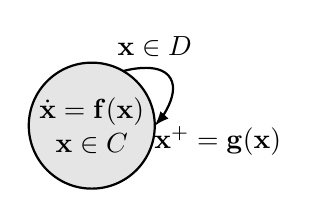
\begin{tikzpicture}
	%
	\fill[gray!20, draw = black,thick] (0,0) circle (0.8cm);
	%	
	\draw (0,0) node[align = center](flow)  {$\dot{\x} = \mathbf{\mathbf{f}}(\x)$\\$\x\in\C$};
	%
	\draw [thick,-latex] plot [smooth, tension=1.2] coordinates { (.4,0.69282) (1,.6) (.8cm,0)};
	%
	\draw (1.6,-0.2) node {$\x^+ = \mathbf{g}(\x)$};
	\draw (.8,1) node {$\x\in\D$};
	%
	\end{tikzpicture}
	\caption[Hybrid automata representiation of the system.]{Hybrid automata: Conceptual representation of the hybrid system $\Ha$ characterized by a single flow map $f$ and one jump map $g$. Only one state and one reset branch are needed to picture the behaviour of the system.}
	\label{fig:HA}
	%\vspace{-5mm}
\end{figure}
%

Let us suppose that the flow map $\mathbf{\mathbf{f}}$ and the jump map $\mathbf{g}$ depend on two sets of \textit{unknown parameters} $\bm{\bm{\alpha}}\in\R^{m_\mathbf{f}}$ and $\bm{\bm{\beta}}\in\R^{m_g}$, i.e.
\[\mathbf{\mathbf{f}} = \mathbf{\mathbf{f}}(\x,\bm{\alpha})\qquad \mathbf{g} = \mathbf{g}(\x,\bm{\beta})\]
and that no \textit{a priori} knowledge of both, the flow set $\C$ and the jump set $\D$ , is available.
Assume that the system is observable, i.e. it is possible to measure and collect samples of the state $\x$.

In order to correctly simulate the system or design a controller for it, it is necessary to identify the parameters in $\bm{\alpha}$, $\bm{\beta}$ and estimate the sets $\C$ and $\D$ from measurements of the state $\x$.

Hereafter, the basic assumptions required to develop the proposed identification method are presented.
Firstly, as a very general hypothesis, both the flow and jump maps are assumed to be linear in the parameters. However, $f$ and $g$ are usually nonlinear with respect to the states.
Thanks to this assumption, it is possible to employ linear identification techniques to estimate the unknown parameters. 
\begin{assum}[Linearity in the parameters]\label{ass:1}
	The maps $f$ and $g$ are linear {with respect to constant} parameters collected in the vectors $\bm{\alpha}\in\R^{m_\mathbf{f}}$ and $\bm{\beta}\in\R^{m_j}$ respectively, i.e., there exist $\bm{\Phi}:\R^{n}\rightarrow\R^{n\times m_f}$ and $\bm{\Psi}:\R^{n}\rightarrow\R^{n\times m_j}$ such that
	\begin{equation*}
	%
	\left\{ 
	\begin{matrix*}[l]\vspace{1pt}
	%
	\dot{\x} = \mathbf{\mathbf{f}}(\x)= \bm{\Phi}(\x)\bm{\alpha}&&\x\in\C\\
	\x^+ = \mathbf{g}(\x)=\bm{\Psi}(\x)\bm{\beta}&&\x\in\D
	%
	\end{matrix*}
	\right.
	%
	\end{equation*}
	{%\color{red} Answer to reviewer \#2 (6)\\
	The maps $\bm{\Phi}$, $\bm{\Psi}$ are assumed to be known a priori.
	} 
\end{assum}
%
The second assumption deals with the regularity of the flow map. %From now on, we denote with $\|\cdot\|$ the 2-norm of a vector.%Another important assumption, is requiring the smoothness and the Lischitzness of the flow map. This will result to be a fundamental hypothesis for the identification procedure. 
\begin{assum}[Smoothness and Lipschitzness of the flow map]\label{ass:2}
The following properties hold for the flow map $\mathbf{\mathbf{f}}$:
\begin{itemize}
	\item[$i)$]  $\mathbf{\mathbf{f}}$ is globally Lipschitz continuous on $\C$, i.e., there exists a constant $k\geq 0$ such that
	\[\forall\x_1,\x_2\in\C\quad\|\mathbf{\mathbf{f}}(\x_1)-\mathbf{\mathbf{f}}(\x_2)\|_2\leq k \|\x_1-\x_2\|_2~. \]
	$k$ is referred as the \textit{Lipschitz constant};
	\item[ii)] $\mathbf{\mathbf{f}}$ is differentiable almost everywhere in $\C$;
	\item[iii)] $\mathbf{\mathbf{f}}$ admits a fixed point in the origin which is inside $\C$, i.e. $\mathbf{\mathbf{f}}(\mymathbb{0}_n)=\mymathbb{0}_n$, $\{\mymathbb{0}_n\}\in\C$.
\end{itemize} 
\end{assum}

\clearpage
%%%%%%%%%%%%%%%%%%%%%%%%%%%%%%%%%%%%%%%%%%%%%%%%%%%%%%%%%%%%%%%%%%%%%%%%%%%%
\section{Jump Detection}\label{JumpD}
%
\begin{defn}[Euler derivative norm]
	Given the hybrid system $(\mathbf{\mathbf{f}},~\mathbf{g},~\C,~\D)$ and a time interval $\delta t>0$, the norm of the Euler derivative of the state is defined as
	\[D_{\delta t}\x(t)= \frac{\|\x(t)-\x(t-\delta t)\|_2}{\delta t}\]
\end{defn}
%
\begin{defn}[Bounded-norm Euler derivative]
	The Euler derivative of a hybrid system $(\mathbf{\mathbf{f}},~\mathbf{g},~\C,~\D)$ has bounded--norm if there exists $\tau(t)\geq 0$ such that
	\[\forall\delta t>0,t\in\R^+~\land~\forall \x\in\C\quad\quad D_{\delta t}\x(t)\leq\tau\]
\end{defn}
%

\begin{thm}[Criteria for the norm bound of the Euler derivative]\label{thm:criteria}
   	%
   	Consider the hybrid system
   	$(\mathbf{\mathbf{f}},~\mathbf{g},~\C,~\D)$. If $\mathbf{\mathbf{f}}(\x)$ satisfies
   	Assumption \ref{ass:2}\footnote{Notice that Assumption \ref{ass:2}($ii$) is
   	not necessary for Theorem \ref{thm:criteria}. However, it will become of fundamental
   	importance later on.} and $\x(t)\in \C ~\forall t \in [t-\delta t,t]$,
   	then the system has bounded--norm Euler derivative with upper bound
	%
	\begin{equation}\label{eq:bound}
		\tau(t)=\frac{1}{\delta t}\int_{t-\delta t}^{t}k\|\x(s)\|_2ds
	\end{equation}
	%
\end{thm}
%
\proof
    %
    Since
    \begin{equation}
        \dot{\x} = \mathbf{\mathbf{f}}(\x)\quad\forall\x\in\C, 
    \end{equation}
    integrating both sides of the equation between $t-\delta t$ and $t$, yields
    %
    \begin{equation}
        \x(t)-\x(t-\delta t) = \int_{t-\delta t}^{t}\mathbf{\mathbf{f}}(\x(s))ds
    \end{equation}
    %
    Therefore,
    %
    \begin{equation}%\label{eq:dtdb}
	    D_{\delta t}\x(t)=\frac{1}{\delta t}\|\x(t)-\x(t-\delta t)\|_2 = \frac{1}{\delta t}\left\lVert\int_{t-\delta t}^{t}\mathbf{\mathbf{f}}(\x(s))ds~\right\rVert_2
    \end{equation}
    %
    Considering the right hand side of the equation, it follows that
    %
    \begin{equation}
        \frac{1}{\delta t}\left\lVert\int_{t-\delta t}^{t}\mathbf{\mathbf{f}}(\x(s))ds~\right\rVert_2\leq\frac{1}{\delta t}\int_{t-\delta t}^{t}\|\mathbf{\mathbf{f}}(\x(s))\|_2ds
    \end{equation}
    %
    Since $f$ is globally Lipschitz in $\C$ and $\mathbf{\mathbf{f}}(\mymathbb{0}_n) = \mymathbb{0}_n$,
    %
    \begin{align}
	    \frac{1}{\delta t}\int_{t-\delta t}^{t}\|\mathbf{\mathbf{f}}(\x(s))\|_2ds &= \frac{1}{\delta t}\int_{t-\delta t}^{t}\|\mathbf{\mathbf{f}}(\x(s))-\mathbf{\mathbf{f}}(\mymathbb{0}_n)\|_2ds\\
	    &\leq\frac{1}{\delta t}\int_{t-\delta t}^{t}k\|\x(s)\|_2ds<\infty
    \end{align}
    %
    where $k$ is the Lipschitz constant. Thus, there exists a $\tau\geq 0$ such that, for all $t$, it holds
    %
    \begin{equation}
        D_{\delta t}\x(t)\leq\frac{1}{\delta t}\int_{t-\delta t}^{t}k\|\x(s)\|_2ds\triangleq\tau(t,\delta t)
    \end{equation}
    The above integral is always limited since, from global Lipschitz continuity of $\mathbf{\mathbf{f}}(\cdot)$, global existence of trajectories $\x(t)$ is assured in $\C$. It follows that on any compact time interval, $[t-\delta t,t]$, where the state does not leave the flow set, the quantity
    %
    \begin{equation}
        \int_{t- \delta t}^{t}\|\x(s)\|_2ds
    \end{equation}
    %
    is limited, providing the result.\\
    %
    $\blacksquare$
    %
\endproof
%
From now on let us refer to $\tau(t)$ as the \textit{smoothness bound}.
%
\begin{exmp}\label{ex:hsid1}
    %
	Consider an hybrid system with the flow described by 
	%
	\begin{equation}
	    \dot{x}={{f}}(x)=\sin(x)\quad x\in\C
	\end{equation}
	%
	where $\C\triangleq[0,2\pi]$. $f$ clearly satisfies Assumption \ref{ass:2} and its Lipschitz constant $k$ can be found as
	%
	\begin{equation}
	    k=\sup\limits_{x\in\C}\left\|\frac{d {f}}{dx}\right\|_2=\sup\limits_{x\in\C}\|\cos(x)\|_2=1
	\end{equation}
	%
	Furthermore, the solution of the ordinary differential equation with $x(0)=x_0$ is\
	%
	\begin{equation}
	    x(t)= 2\tan^{-1}\left(e^{t-\ln(\cot(x_0/2))}\right)
	\end{equation}
	%
	Since ${\mathbf{f}}(0)=0$ ($\{0\}\in\C$) Theorem \ref{thm:criteria} holds and, for any $\delta t>0$ yields
	%
	\begin{equation}\label{eq:exmp_sb}
	    D_{\delta t}x(t)=\frac{1}{\delta t}\|x(t)-x(t-\delta t)\|\leq\frac{1}{\delta t}\int_{t-\delta t}^{t}\|x(s)\|_2ds=\tau(t)
	\end{equation}
	%
	Figure \ref{fig:ex1} shows in a numerical example with $x_0=10^{-2}$ and $\delta t = 0.5$. 
	%
	\begin{figure}[!t]
        \centering
        %
\definecolor{mycolor1}{rgb}{0.00000,0.44706,0.74118}%
%
\begin{tikzpicture}

\begin{axis}
[%
width=8cm,
height=4.5cm,
at={(0.614in,0.251in)},
scale only axis,
xmin=0.5,
xmax=10,
ymin=0,
ymax=3.12343333205421,
axis background/.style={fill=white},
xlabel=$t$,ylabel={$x(t),$ $D_{\delta t}x(t)$, $\tau(t)$}, 
legend style={legend cell align=left, align=left, draw=white!15!black, {at={(2.5cm,3.2cm)}}
}
]
\addplot [color=black, line width=1.5pt]
  table[row sep=crcr]{%
0.5	0.0164869766336163\\
0.521939953810624	0.0168526802942833\\
0.543879907621247	0.0172264949765504\\
0.565819861431871	0.0176086005231329\\
0.587759815242494	0.0179991807606994\\
0.609699769053118	0.0183984235878792\\
0.631639722863741	0.0188065210651958\\
0.653579676674365	0.0192236695069702\\
0.675519630484988	0.0196500695752333\\
0.697459584295612	0.0200859263756921\\
0.719399538106236	0.020531449555791\\
0.741339491916859	0.0209868534049148\\
0.763279445727483	0.0214523569567771\\
0.785219399538106	0.0219281840940402\\
0.80715935334873	0.0224145636552135\\
0.829099307159353	0.0229117295438787\\
0.851039260969977	0.0234199208402892\\
0.8729792147806	0.0239393819153934\\
0.894919168591224	0.0244703625473337\\
0.916859122401848	0.0250131180404692\\
0.938799076212471	0.0255679093469781\\
0.960739030023095	0.0261350031910889\\
0.982678983833718	0.0267146721959971\\
1.00461893764434	0.0273071950135207\\
1.02655889145497	0.0279128564565499\\
1.04849884526559	0.0285319476343487\\
1.07043879907621	0.0291647660907644\\
1.09237875288684	0.0298116159454041\\
1.11431870669746	0.0304728080378367\\
1.13625866050808	0.0311486600748806\\
1.15819861431871	0.0318394967810383\\
1.18013856812933	0.0325456500521386\\
1.20207852193995	0.0332674591122494\\
1.22401847575058	0.0340052706739243\\
1.2459584295612	0.0347594391018466\\
1.26789838337182	0.0355303265799362\\
1.28983833718245	0.0363183032819838\\
1.31177829099307	0.037123747545879\\
1.3337182448037	0.0379470460514997\\
1.35565819861432	0.038788594002329\\
1.37759815242494	0.0396487953108679\\
1.39953810623557	0.0405280627879132\\
1.42147806004619	0.0414268183357682\\
1.44341801385681	0.0423454931454554\\
1.46535796766744	0.0432845278980026\\
1.48729792147806	0.0442443729698699\\
1.50923787528868	0.0452254886425893\\
1.53117782909931	0.0462283453166861\\
1.55311778290993	0.0472534237299525\\
1.57505773672055	0.0483012151801435\\
1.59699769053118	0.0493722217521641\\
1.6189376443418	0.0504669565498182\\
1.64087759815242	0.051585943932187\\
1.66281755196305	0.0527297197547054\\
1.68475750577367	0.0538988316150044\\
1.7066974595843	0.0550938391035848\\
1.72863741339492	0.0563153140593882\\
1.75057736720554	0.0575638408303287\\
1.77251732101617	0.0588400165388478\\
1.79445727482679	0.0601444513525529\\
1.81639722863741	0.0614777687599975\\
1.83833718244804	0.062840605851659\\
1.86027713625866	0.0642336136061679\\
1.88221709006928	0.065657457181839\\
1.90415704387991	0.0671128162135495\\
1.92609699769053	0.0686003851150112\\
1.94803695150115	0.0701208733864719\\
1.96997690531178	0.0716750059278844\\
1.9919168591224	0.0732635233575704\\
2.01385681293303	0.0748871823364057\\
2.03579676674365	0.0765467558975437\\
2.05773672055427	0.0782430337816902\\
2.0796766743649	0.0799768227779342\\
2.10161662817552	0.0817489470701315\\
2.12355658198614	0.0835602485888314\\
2.14549653579677	0.0854115873687232\\
2.16743648960739	0.0873038419115765\\
2.18937644341801	0.0892379095546294\\
2.21131639722864	0.0912147068443768\\
2.23325635103926	0.0932351699156896\\
2.25519630484988	0.0953002548761887\\
2.27713625866051	0.0974109381957793\\
2.29907621247113	0.0995682171012352\\
2.32101616628175	0.101773109975709\\
2.34295612009238	0.104026656763022\\
2.364896073903	0.106329919376569\\
2.38683602771363	0.108683982112654\\
2.40877598152425	0.111089952068044\\
2.43071593533487	0.113548959561518\\
2.4526558891455	0.116062158559139\\
2.47459584295612	0.118630727102971\\
2.49653579676674	0.121255867742917\\
2.51847575057737	0.123938807971341\\
2.54041570438799	0.126680800660069\\
2.56235565819861	0.129483124499368\\
2.58429561200924	0.132347084438433\\
2.60623556581986	0.13527401212688\\
2.62817551963049	0.138265266356696\\
2.65011547344111	0.141322233504056\\
2.67205542725173	0.144446327970363\\
2.69399538106236	0.147638992621791\\
2.71593533487298	0.150901699226603\\
2.7378752886836	0.154235948889392\\
2.75981524249423	0.157643272481389\\
2.78175519630485	0.161125231065855\\
2.80369515011547	0.164683416317551\\
2.8256351039261	0.16831945093516\\
2.84757505773672	0.172034989045488\\
2.86951501154734	0.175831716598145\\
2.89145496535797	0.179711351749354\\
2.91339491916859	0.1836756452334\\
2.93533487297921	0.187726380720156\\
2.95727482678984	0.191865375156994\\
2.97921478060046	0.196094479093277\\
3.00115473441109	0.200415576985517\\
3.02309468822171	0.204830587481131\\
3.04503464203233	0.209341463678618\\
3.06697459584296	0.213950193361813\\
3.08891454965358	0.218658799205738\\
3.1108545034642	0.223469338951413\\
3.13279445727483	0.228383905546809\\
3.15473441108545	0.23340462725097\\
3.17667436489607	0.238533667698146\\
3.1986143187067	0.243773225918574\\
3.22055427251732	0.249125536312371\\
3.24249422632794	0.254592868572785\\
3.26443418013857	0.260177527554832\\
3.28637413394919	0.265881853085144\\
3.30831408775982	0.271708219708606\\
3.33025404157044	0.277659036367133\\
3.35219399538106	0.283736746005699\\
3.37413394919169	0.289943825100474\\
3.39607390300231	0.296282783103668\\
3.41801385681293	0.302756161799431\\
3.43995381062356	0.30936653456488\\
3.46189376443418	0.31611650553006\\
3.4838337182448	0.32300870863038\\
3.50577367205543	0.33004580654478\\
3.52771362586605	0.337230489512626\\
3.54965357967667	0.344565474022046\\
3.5715935334873	0.352053501362168\\
3.59353348729792	0.359697336031447\\
3.61547344110854	0.367499763994026\\
3.63741339491917	0.375463590775833\\
3.65935334872979	0.383591639391895\\
3.68129330254042	0.391886748096127\\
3.70323325635104	0.400351767944704\\
3.72517321016166	0.408989560163916\\
3.74711316397229	0.417802993313332\\
3.76905311778291	0.426794940234962\\
3.79099307159353	0.435968274779093\\
3.81293302540416	0.445325868297436\\
3.83487297921478	0.454870585894309\\
3.8568129330254	0.464605282426669\\
3.87875288683603	0.474532798243983\\
3.90069284064665	0.484655954659209\\
3.92263279445728	0.494977549142467\\
3.9445727482679	0.505500350229423\\
3.96651270207852	0.516227092136957\\
3.98845265588915	0.527160469079279\\
4.01039260969977	0.538303129278488\\
4.03233256351039	0.549657668664381\\
4.05427251732102	0.561226624259419\\
4.07621247113164	0.573012467245858\\
4.09815242494226	0.585017595713446\\
4.12009237875289	0.597244327087549\\
4.14203233256351	0.60969489023922\\
4.16397228637413	0.622371417280618\\
4.18591224018476	0.635275935051172\\
4.20785219399538	0.648410356302135\\
4.229792147806	0.661776470589565\\
4.25173210161663	0.675375934888406\\
4.27367205542725	0.689210263943143\\
4.29561200923787	0.703280820373475\\
4.3175519630485	0.717588804556675\\
4.33949191685912	0.732135244311617\\
4.36143187066975	0.746920984413016\\
4.38337182448037	0.761946675968038\\
4.40531177829099	0.777212765691272\\
4.42725173210162	0.792719485117913\\
4.44919168591224	0.808466839798968\\
4.47113163972286	0.824454598526284\\
4.49307159353349	0.840682282639177\\
4.51501154734411	0.857149155468356\\
4.53695150115473	0.873854211976691\\
4.55889145496536	0.890796168659977\\
4.58083140877598	0.90797345377438\\
4.6027713625866	0.925384197960318\\
4.62471131639723	0.943026225335438\\
4.64665127020785	0.96089704513167\\
4.66859122401848	0.978993843953317\\
4.6905311778291	0.997313478734424\\
4.71247113163972	1.01585247047444\\
4.73441108545035	1.03460699883115\\
4.75635103926097	1.05357289764916\\
4.77829099307159	1.07274565150059\\
4.80023094688222	1.09212039331212\\
4.82217090069284	1.11169190314943\\
4.84411085450346	1.13145460822521\\
4.86605080831409	1.15140258419227\\
4.88799076212471	1.17152955777638\\
4.90993071593534	1.19182891079657\\
4.93187066974596	1.21229368561235\\
4.95381062355658	1.23291659202809\\
4.97575057736721	1.25369001567483\\
4.99769053117783	1.27460602787942\\
5.01963048498845	1.29565639701894\\
5.04157043879908	1.31683260134701\\
5.0635103926097	1.33812584326594\\
5.08545034642032	1.35952706500622\\
5.10739030023095	1.3810269656622\\
5.12933025404157	1.40261601952019\\
5.15127020785219	1.42428449560284\\
5.17321016166282	1.44602247834191\\
5.19515011547344	1.46781988928006\\
5.21709006928406	1.48966650969198\\
5.23903002309469	1.5115520040055\\
5.26096997690531	1.53346594389509\\
5.28290993071594	1.5553978329129\\
5.30484988452656	1.57733713151661\\
5.32678983833718	1.59927328234937\\
5.34872979214781	1.62119573562416\\
5.37066974595843	1.64309397446368\\
5.39260969976905	1.66495754004768\\
5.41454965357968	1.6867760564214\\
5.4364896073903	1.70853925482266\\
5.45842956120092	1.73023699739026\\
5.48036951501155	1.75185930012297\\
5.50230946882217	1.77339635496627\\
5.52424942263279	1.79483855091315\\
5.54618937644342	1.8161764940153\\
5.56812933025404	1.83740102621215\\
5.59006928406466	1.85850324289671\\
5.61200923787529	1.87947450914953\\
5.63394919168591	1.9003064745844\\
5.65588914549654	1.9209910867622\\
5.67782909930716	1.941520603142\\
5.69976905311778	1.96188760155069\\
5.72170900692841	1.98208498916477\\
5.74364896073903	2.00210601000943\\
5.76558891454965	2.02194425099092\\
5.78752886836028	2.04159364648878\\
5.8094688221709	2.06104848154354\\
5.83140877598152	2.08030339368453\\
5.85334872979215	2.09935337344974\\
5.87528868360277	2.1181937636565\\
5.8972286374134	2.13682025748759\\
5.91916859122402	2.15522889546172\\
5.94110854503464	2.17341606136161\\
5.96304849884527	2.19137847719531\\
5.98498845265589	2.20911319726849\\
6.00692840646651	2.22661760144651\\
6.02886836027714	2.24388938768539\\
6.05080831408776	2.26092656391023\\
6.07274826789838	2.27772743931873\\
6.09468822170901	2.29429061518559\\
6.11662817551963	2.31061497524142\\
6.13856812933025	2.32669967569721\\
6.16050808314088	2.34254413498228\\
6.1824480369515	2.35814802326026\\
6.20438799076212	2.37351125178428\\
6.22632794457275	2.38863396214847\\
6.24826789838337	2.4035165154892\\
6.270207852194	2.41815948168557\\
6.29214780600462	2.43256362860435\\
6.31408775981524	2.44672991143104\\
6.33602771362587	2.46065946212446\\
6.35796766743649	2.47435357902858\\
6.37990762124711	2.4878137166716\\
6.40184757505774	2.50104147577866\\
6.42378752886836	2.5140385935212\\
6.44572748267898	2.52680693402268\\
6.46766743648961	2.53934847913721\\
6.48960739030023	2.55166531951509\\
6.51154734411085	2.56375964596613\\
6.53348729792148	2.57563374112942\\
6.5554272517321	2.58728997145586\\
6.57736720554272	2.59873077950758\\
6.59930715935335	2.60995867657656\\
6.62124711316397	2.62097623562283\\
6.6431870669746	2.6317860845315\\
6.66512702078522	2.6423908996858\\
6.68706697459584	2.65279339985278\\
6.70900692840647	2.66299634037674\\
6.73094688221709	2.6730025076747\\
6.75288683602771	2.68281471402752\\
6.77482678983834	2.69243579265925\\
6.79676674364896	2.70186859309718\\
6.81870669745958	2.7111159768042\\
6.84064665127021	2.72018081307479\\
6.86258660508083	2.72906597518599\\
6.88452655889146	2.73777433679389\\
6.90646651270208	2.74630876856669\\
6.9284064665127	2.7546721350448\\
6.95034642032333	2.76286729171872\\
6.97228637413395	2.77089708231537\\
6.99422632794457	2.77876433628363\\
7.0161662817552	2.78647186646993\\
7.03810623556582	2.79402246697496\\
7.06004618937644	2.80141891118266\\
7.08198614318707	2.80866394995287\\
7.10392609699769	2.81576030996932\\
7.12586605080831	2.82271069223468\\
7.14780600461894	2.82951777070487\\
7.16974595842956	2.836184191055\\
7.19168591224018	2.84271256956935\\
7.21362586605081	2.84910549214854\\
7.23556581986143	2.85536551342688\\
7.25750577367206	2.86149515599332\\
7.27944572748268	2.86749690970981\\
7.3013856812933	2.8733732311209\\
7.32332563510393	2.87912654294892\\
7.34526558891455	2.88475923366919\\
7.36720554272517	2.89027365716006\\
7.3891454965358	2.89567213242265\\
7.41108545034642	2.9009569433658\\
7.43302540415704	2.90613033865145\\
7.45496535796767	2.91119453159632\\
7.47690531177829	2.91615170012583\\
7.49884526558891	2.92100398677642\\
7.52078521939954	2.92575349874252\\
7.54272517321016	2.93040230796501\\
7.56466512702078	2.93495245125758\\
7.58660508083141	2.9394059304683\\
7.60854503464203	2.94376471267321\\
7.63048498845266	2.94803073039941\\
7.65242494226328	2.95220588187513\\
7.6743648960739	2.95629203130415\\
7.69630484988453	2.96029100916263\\
7.71824480369515	2.964204612516\\
7.74018475750577	2.9680346053541\\
7.7621247113164	2.97178271894256\\
7.78406466512702	2.97545065218887\\
7.80600461893764	2.97904007202137\\
7.82794457274827	2.98255261377968\\
7.84988452655889	2.98598988161526\\
7.87182448036952	2.98935344890064\\
7.89376443418014	2.99264485864618\\
7.91570438799076	2.99586562392321\\
7.93764434180139	2.99901722829245\\
7.95958429561201	3.00210112623681\\
7.98152424942263	3.00511874359753\\
8.00346420323326	3.00807147801295\\
8.02540415704388	3.01096069935902\\
8.0473441108545	3.01378775019087\\
8.06928406466513	3.01655394618481\\
8.09122401847575	3.01926057658004\\
8.11316397228637	3.02190890461966\\
8.135103926097	3.02450016799025\\
8.15704387990762	3.02703557925978\\
8.17898383371825	3.02951632631319\\
8.20092378752887	3.03194357278545\\
8.22286374133949	3.03431845849152\\
8.24480369515012	3.0366420998531\\
8.26674364896074	3.03891559032168\\
8.28868360277136	3.04114000079776\\
8.31062355658199	3.04331638004589\\
8.33256351039261	3.04544575510542\\
8.35450346420323	3.04752913169665\\
8.37644341801386	3.04956749462227\\
8.39838337182448	3.05156180816401\\
8.4203233256351	3.05351301647417\\
8.44226327944573	3.05542204396211\\
8.46420323325635	3.05728979567552\\
8.48614318706698	3.05911715767632\\
8.5080831408776	3.06090499741131\\
8.53002309468822	3.06265416407722\\
8.55196304849885	3.06436548898047\\
8.57390300230947	3.06603978589127\\
8.59584295612009	3.06767785139228\\
8.61778290993072	3.06928046522164\\
8.63972286374134	3.07084839061053\\
8.66166281755196	3.07238237461513\\
8.68360277136259	3.073883148443\\
8.70554272517321	3.07535142777402\\
8.72748267898383	3.07678791307573\\
8.74942263279446	3.07819328991328\\
8.77136258660508	3.07956822925385\\
8.7933025404157	3.08091338776572\\
8.81524249422633	3.08222940811197\\
8.83718244803695	3.0835169192388\\
8.85912240184757	3.08477653665866\\
8.8810623556582	3.08600886272811\\
8.90300230946882	3.08721448692054\\
8.92494226327945	3.08839398609373\\
8.94688221709007	3.08954792475244\\
8.96882217090069	3.09067685530599\\
8.99076212471132	3.09178131832085\\
9.01270207852194	3.09286184276847\\
9.03464203233256	3.09391894626826\\
9.05658198614319	3.09495313532583\\
9.07852193995381	3.09596490556667\\
9.10046189376443	3.09695474196507\\
9.12240184757506	3.09792311906872\\
9.14434180138568	3.09887050121869\\
9.16628175519631	3.09979734276515\\
9.18822170900693	3.10070408827869\\
9.21016166281755	3.10159117275745\\
9.23210161662818	3.1024590218301\\
9.2540415704388	3.10330805195464\\
9.27598152424942	3.10413867061325\\
9.29792147806005	3.10495127650315\\
9.31986143187067	3.10574625972355\\
9.34180138568129	3.10652400195879\\
9.36374133949192	3.10728487665774\\
9.38568129330254	3.10802924920949\\
9.40762124711316	3.10875747711543\\
9.42956120092379	3.10946991015775\\
9.45150115473441	3.11016689056453\\
9.47344110854504	3.1108487531713\\
9.49538106235566	3.1115158255793\\
9.51732101616628	3.11216842831046\\
9.5392609699769	3.11280687495908\\
9.56120092378753	3.11343147234043\\
9.58314087759815	3.11404252063616\\
9.60508083140878	3.11464031353668\\
9.6270207852194	3.11522513838061\\
9.64896073903002	3.11579727629118\\
9.67090069284065	3.11635700230989\\
9.69284064665127	3.11690458552723\\
9.71478060046189	3.11744028921076\\
9.73672055427252	3.11796437093035\\
9.75866050808314	3.11847708268087\\
9.78060046189376	3.11897867100228\\
9.80254041570439	3.11946937709707\\
9.82448036951501	3.11994943694534\\
9.84642032332563	3.12041908141734\\
9.86836027713626	3.12087853638366\\
9.89030023094688	3.12132802282305\\
9.91224018475751	3.12176775692797\\
9.93418013856813	3.12219795020786\\
9.95612009237875	3.12261880959024\\
9.97806004618938	3.12303053751959\\
10	3.12343333205421\\
};
\addlegendentry{$x(t)$}

\addplot [color=black, dashed, line width=1.5pt]
  table[row sep=crcr]{%
0.5	0.0129739532672325\\
1	0.0213887890512713\\
1.5	0.0352567873322842\\
2	0.0580956390510823\\
2.5	0.0956360621103947\\
3	0.157020421985983\\
3.5	0.255987827542454\\
4	0.409638066069622\\
4.5	0.625715552757503\\
5	0.861918250157168\\
5.5	0.98863584781858\\
6	0.899962647892008\\
6.5	0.67261377588965\\
7	0.446772389026869\\
7.5	0.280897000179203\\
8	0.172706018049722\\
8.5	0.105282699117182\\
9	0.0639765998270478\\
9.5	0.0388304878259991\\
10	0.0235578491571697\\
};
\addlegendentry{$D_{\delta t}x(t)$}

\addplot [color=mycolor1, dotted, line width=1.5pt]
  table[row sep=crcr]{%
0.5	0.0129743401088805\\
1	0.0213905225830566\\
1.5	0.0352645543856456\\
2	0.0581304230457569\\
2.5	0.0957916430235894\\
3	0.157713935460563\\
3.5	0.259051089600454\\
4	0.422847086960148\\
4.5	0.679352698203029\\
5	1.05251847669386\\
5.5	1.52300062799024\\
6	2.00392136983382\\
6.5	2.39952510759622\\
7	2.6773929765478\\
7.5	2.85662226418524\\
8	2.96796161927934\\
8.5	3.03610220157572\\
9	3.07756958574395\\
9.5	3.10275178811816\\
10	3.11803248810844\\
};
\addlegendentry{$\tau(t)$}

\end{axis}
\end{tikzpicture}%

        \caption[Example \ref{ex:hsid1}: Time evolution of the state, Euler derivative norm and smoothness bound.]{Example \ref{ex:hsid1}. Time evolution of $x(t)$, $D_{\delta t}x(t)$, $\tau(t)$ for $x_0=10^{-2}$ and $\delta t=0.5$. This figure shows an application example of Theorem \ref{thm:criteria}. Notice that, as predicted by (\ref{eq:exmp_sb}), along the whole trajectory $D_{\delta t}x(t)$ is bounded from above by $\tau(t)$.}
        \label{fig:ex1}
    \end{figure}
    %
\end{exmp}
Thanks to Assumption \ref{ass:2} and the criteria provided by Theorem \ref{thm:criteria}, any jump, i.e. state discontinuities, can be detected from a series of state measurements by inspecting the norm of the Euler derivative. In particular, the system can be considered to be jumping if $D_{\delta t}\x(t)$ is above an empirically estimated \textit{smoothness bound} $\hat{\tau}(t)$
%
{%\color{red} 
and the following assumption is always satisfied.%
\begin{assum}[Discontinuities and sampling time]\label{ass:3}
    For the chosen $\delta t$ and $\hat{\tau}$, it holds:
    \begin{itemize}
        \item[$i)$] $\mathbf{g}(\x)\in\C~~\forall\x\in\D$;
        \item[$ii)$] If there exists a time instant $s\in[t-\delta t,t]$ such that $\x(s)\in\D$, then $s$ is unique; %$\exists ! ~s:~\forall s\in[t-\delta t,t]~~\x(s)\in\D$;
        \item[$iii)$] Let $\x(s)\in\D,~s\in(t-\delta t,t)$. Then,    
        %
        \begin{equation}\label{eq:ass3.3}
            \D_{\delta t} \x(t)\geq \hat{\tau}(t,\delta t).
        \end{equation}
        %
    \end{itemize}
\end{assum}
}
%
It is worth to clarify that Assumption \ref{ass:3}($i$) is needed to ensure that after a jump, the state will go back to the flow set. Moreover,  \ref{ass:3}($ii$) ensures that the sampling time is small enough such that only one jump may happen within one time interval. Finally, \ref{ass:3}($iii$) requires that the sampling time and the estimated smoothness bounds are chose such that a jump can be detected looking at the Euler derivative norm.

% \textcolor{red}{
% Note that (\ref{eq:ass3.3}) becomes
% %
% \begin{align}
%      \D_{\delta t} \x(t) &= \frac{\|\x(t)-\x(t-\delta t)\|_2}{\delta t} =\\
%                          &= \dfrac{1}{\delta t}\left\|\int_s^t\mathbf{\mathbf{f}}(\x(v))dv + \mathbf{g}(\x(s))-\x(t-\delta t)\right\|_2 =\\
%                          &= \dfrac{1}{\delta t}\left\|\int_s^t\mathbf{\mathbf{f}}(\x(v))dv + \mathbf{g}(\x(s))-\x(s) + \int_{t-\delta t}^s\mathbf{\mathbf{f}}(\x(v))dv\right\|_2 = \\
%                          &= \dfrac{1}{\delta t}\left\|\int_s^t\mathbf{\mathbf{f}}(\x(v))dv + \mathbf{g}(\x(s))-\x(s) + \int_{t-\delta t}^s\mathbf{\mathbf{f}}(\x(v))dv\right\|_2
% \end{align}
% %
% and if $g(\x)\neq \x$ it holds
% %
% \begin{equation}
%     \lim_{\delta t\rightarrow 0} \dfrac{1}{\delta t}\left\|\int_s^t\mathbf{\mathbf{f}}(\x(v))dv + \mathbf{g}(\x(s))-\x(t-\delta t)\right\|_2 = \infty
% \end{equation}
% %
% }
%
Therefore, a \textit{jump detection function} can be defined as
%
\begin{equation}
    \gamma(t)\triangleq \left\{ 
        \begin{matrix*}[l]\vspace{1pt}
            %
            0&&\dfrac{1}{\delta t}\|\x(t)-\x(t-\delta t)\|_2 \leq \hat{\tau}(t)\\
            1&&\text{otherwise}
            %
        \end{matrix*}
    \right.
\end{equation}
%	
which is zero during the flows of the system and assumes the value 1 during the jumps.

At any instant of time $\gamma(t)$ allows to determine whether the system is \textit{jumping} of \textit{flowing};
 $\hat{\tau}$ can be adaptively changed as function of the state and/or time.
Note that $\gamma(t)=1$ indicates that the jump just happened and thus the system's state had been inside the jump set $\D$ during the time interval $[t-\delta t,t]$.
%
\begin{rem}
    Assumption \ref{ass:3} ensures two important properties. Firstly, that only one jump is possible between two samples of the state. Secondly, that the discontinuities created by jumps always make the Euler derivative norm to exceed the estimated smoothness bound for the chosen sampling time. 
\end{rem}
%
\clearpage
%%%%%%%%%%%%%%%%%%%%%%%%%%%%%%%%%%%%%%%%%%%%%%%%%%%%%%%%%%%%%%%%%%%%%%%%%%%%%%%%%%%%%
\section{Identification Procedure}\label{Identification}

\subsection{Approximation of the Smoothness Bound}
In order to estimate on-line the smoothness bound (\ref{eq:bound}), it is necessary to approximate the Lipschitz constant $k$ and then numerically integrate the norm of the state between two sampling instants.
At any time instant $t$, the estimated flow map $\hat{\mathbf{f}}(\x,t)$ is defined as
%
\begin{equation}
    \hat{\mathbf{f}}(\x,t)=\bm{\Phi}(\x)\hat{\bm{\alpha}}(t)
\end{equation}
%
where $\hat{\bm{\alpha}}(t)$ is the estimated vector of flow parameters at time $t$. Thanks to Assumption \ref{ass:2}, $\mathbf{f}(\x)$ is differentiable (and so is $\hat{\mathbf{f}}(\x,t)$) and globally Lipschitz on $\C$, the Lipschitz constant will bound from above the supremum of the norm of the Jacobian of $\mathbf{f}(\x)$ in the flow set $\C$:
%
\begin{equation}
    k\geq\sup\limits_{\x\in\C}\left\|\frac{\partial \mathbf{f}(\x)}{\partial\x}\right\|_2.
\end{equation}
%
Since $\mathbf{f}(\x)$ is not known a priori ($\bm{\alpha}$ is unknown), the estimation of $k$ must be carried out employing the estimated flow map $\hat{\mathbf{f}}(\x,t)$. In this paper, as an estimate of the Lipschitz constant, the following quantity is considered:
%
\begin{equation}
    \hat{k} = r\sup\limits_{\x\in\C}\left\|\frac{\partial \hat{\mathbf{f}}(\x,t)}{\partial\x}\right\|_2\quad r>1.
\end{equation}
%
Therefore, the estimated smoothness bound $\hat{\tau}(t)$ is given by
%
\begin{align}
    \hat{\tau}(t) &= \frac{\hat{k}}{\delta t}\int_{t-\delta t}^{t}\|\x(s)\|_2ds =\\
                  &= \frac{r}{\delta t}\sup\limits_{\x\in\C}\left\|\frac{\partial \hat{\mathbf{f}}(\x,t)}{\partial\x}\right\|_2\int_{t-\delta t}^{t}\|\x(s)\|_2ds.
\end{align}
%
Notice that the integral below must be computed numerically. A possible simple choice is to use the first order Newton-Cotes formula (trapezoidal rule). This would yield to the following approximation of $\hat{\tau}(t)$
%
\begin{align}
    \hat{\tau}(t) &=\frac{r}{\delta t}\sup\limits_{\x\in\C}\left\|\frac{\partial \hat{\mathbf{f}}(\x,t)}{\partial\x}\right\|_2\int_{t-\delta t}^{t}\|\x(s)\|_2ds\\
    \label{eq:htau}
                  &\approx\frac{r}{2}\sup\limits_{\x\in\C}\left\|\frac{\partial \hat{\mathbf{f}}(\x,t)}{\partial\x}\right\|_2\big(\|\x(t)\|_2+\|\x(t-\delta t)\|_2\big).
\end{align}
%
It worths to be observed that with this numerical integration algorithm the estimated smoothness threshold does not explicitly depends on $\delta t$.
Other empirical methods for computing the Lipschitz constant of multivariable functions are presented in \cite{mladineo1986algorithm,Wood1996}. Notice that we do not have any \textit{a priori} knowledge of $\C$ and thus, in equation (\ref{eq:htau}) an approximated flow set $\hat{\C}$  should be employed.
%
{%\color{red} \\ Answer to reviewer \#1 (5), reviewer \#2 (7)
\begin{rem}
    The tuning of the multiplicative constant $r$ should be addressed empirically.
    In fact, it has to be chosen considering a trade off between robustness (high $r$ ensures that $\hat{\tau}(t)\geq\tau(t)$ $\forall t$) and accuracy (low $r$ let $\hat{\tau}$ stay below the peaks of $D_{\delta t}\x(t)$ during jumps, i.e. Assumption 3 would be violated).
\end{rem}
}
%
Thus, the final \textit{jump detection function} becomes
%
\begin{equation}
    \gamma(t)\triangleq \left\{ 
        \begin{matrix*}[l]\vspace{1pt}
            %
            0&&\dfrac{1}{\delta t}\|\x(t)-\x(t-\delta t)\|_2 \leq \dfrac{r}{2}\sup\limits_{\x\in\hat{\C}}\left\|\dfrac{\partial \hat{\mathbf{f}}(\x,t)}{\partial\x}\right\|_2\big(\|\x(t)\|_2+\|\x(t-\delta t)\|_2\big)\\
            1&&\text{otherwise}
            %
        \end{matrix*}
    \right.
\end{equation}
%
\subsection{Parameters Estimation}
%{\color{red}DA FARE}\\
Let us assume to observe the system and measure the state $\x$ with a sampling time $\delta t$. Suppose to collect $N_f$ samples during the flows of the system. %and its derivative $\dot{\x}$ 
It holds:
\begin{equation}\label{eq:linflow}
	\begin{bmatrix}\dot{\x}(t_1)\\\dot{\x}(t_2)\\\vdots\\\dot{\x}(t_{N_\mathbf{f}})\end{bmatrix}=
	\begin{bmatrix}\bm{\Phi}(\x(t_1))\\\bm{\Phi}(\x(t_2))\\\vdots\\\bm{\Phi}(\x(t_{N_\mathbf{f}}))\end{bmatrix}\bm{\alpha}
\end{equation}
Similarly, if $N_j$ samples of the states are collected during jumps, i.e., if $\gamma(t_i)=1$ for all $i = 1,\dots,N_j$, yields
\begin{equation}\label{eq:linjump}
	\begin{bmatrix}{\x}(t_1)\\\x(t_2)\\\vdots\\{\x}(t_{N_j})\end{bmatrix}=
	\begin{bmatrix}\bm{\Psi}(\x(t_1-\delta t))\\\bm{\Psi}(\x(t_2-\delta t))\\\vdots\\\bm{\Psi}(\x(t_{N_j}-\delta t))\end{bmatrix}\bm{\beta}
\end{equation}
%Note that, in general, $\delta t$ might not be constant. 
However, in practice, measurements are always affected by noise and, thus, relations (\ref{eq:linflow}) and (\ref{eq:linjump}) do not hold.
In particular, let's assume that an additive noise, $\tilde{\x}(t_i)$, with zero-mean affects the system, i.e., $\x(t_i)=\bar{\x}(t_i)+\tilde{\x}(t_i)$, where $\bar{\x}(t_i)$ is the true value of the state variable.

Thanks to Assumption \ref{ass:1}, the parameters in $\bm{\alpha}$ and $\bm{\beta}$ can be estimated by linear identification techniques. In fact, both equations,  (\ref{eq:linflow}) and (\ref{eq:linjump}) belong to the error-in-variables (EIV) models:
\begin{equation}
	\yb\approx \mathbf{Xa}
\end{equation}
where $\yb = \bar{\yb}+\tilde{\yb}$ is an output's measurements vector and $\mathbf{X} = \bar{\mathbf{X}}+\tilde{\mathbf{X}}$ is an observation matrix, both comprise of a noiseless part ($\bar{\yb}$, $\bar{\mathbf{X}}$), and  a noisy part ($\tilde{\yb}$, $\tilde{\mathbf{X}}$).
%
{%\color{red}\\Ansewer to Reviewer \#1 (2) [Part 1.]\\
In this linear model, the vector of parameters $\mathbf{a}$ could be estimated by mean of a standard linear estimator \cite{ljung1987system}. The choice of the proper estimation scheme should be done considering how the measurement noise is distributed on the possible state--nonlinearities of $\bm{\Phi}$ and $\bm{\Psi}$.
}%with the recursive least squares (RLS) scheme .

The overall identification experiment is carried out as follows: at each sampling time, the jump detection function is computed. If the system is considered to be flowing, the estimated flow parameter $\hat{\bm{\alpha}}$ is updated and the jump parameter $\hat{\bm{\beta}}$ remains unchanged. On the contrary, if a jump state is detected  $\gamma(t)=1$, the jump parameter $\hat{\bm{\beta}}$ will be updated and the flow parameters $\hat{\bm{\alpha}}$ will be unchanged.

Notice that, in order to update the flow parameters $\hat{\bm{\alpha}}$ according to the 
% 
{chosen linear estimation scheme}, the knowledge of the derivative of the state, $\dot{\x}(t)$, is needed. Since we assume to be able of collecting only samples of the state, this quantity has to be computed numerically (Euler derivative, sliding mode, etc.). 
This cumbersome calculation can be avoided by considering that the  linear relation holds even if it is integrated in an interval of time. In fact,  %This might be computed with a simple backward difference or with any finer numerical differentiation techniques. Besides, this step inevitably introduces errors in the system which leads to imperfect estimations even in the noiseless case. In the noisy case, the situation become even worse since the numerical differentiation would amplify the noise. In order to avoid this kind of problems, it can be shown that the linear relation holds even if it integrated in an interval of time. In fact,
%
\begin{align}
	&\dot{\x}(t)=\bm{\Phi}(\x(t))\bm{\alpha}\\
	\Leftrightarrow\quad&\underbrace{\x(t)-\x(t-\delta t)}_{\delta\x(t)} = 
	\underbrace{\int_{t-\delta t}^{t}\bm{\Phi}(\x(s))ds}_{\bm{\bar{\Phi}}(t)}\bm{\alpha}\\\label{eq:intmod}
	\Leftrightarrow\quad&\delta\x(t)={\bm{\bar{\Phi}}}(t)\bm{\alpha}
\end{align}
% 
This propriety has been exploit in the identification experiments by employing the model (\ref{eq:intmod}).
An overview of the procedure used to update the parameters at time $t$ is presented in Algorithm \ref{alg:HID}.
%
%\setlength{\textfloatsep}{2.5pt}
\begin{algorithm}[!b]
    %
	\caption{Identification of the Hybrid System}\label{alg:HID}
	\begin{algorithmic}[1]
		\State \textbf{Input:} $\hat{\bm{\alpha}}(t-\delta t)$, $\hat{\bm{\beta}}(t-\delta t)$, $\x(t)$, $\x(t-\delta t)$
		\State Compute $\hat{\tau}(t)=\dfrac{r}{2}\sup\limits_{\x\in\C}\left\|\dfrac{\partial \hat{\mathbf{f}}(\x,t)}{\partial\x}\right\|_2\big(\|\x(t)\|_2+\|\x(t-\delta t)\|_2\big)$
		\State Compute $\gamma(t)$
		\If {$\gamma(t)=0$}
		%
		\State $\delta\x(t) = \x(t)-\x(t-\delta t)$,~$\bm{\bar{\Phi}}(t)=\int_{t-\delta t}^{t}\bm{\Phi}(\x(s))ds$
		%
		\State Update $\hat{\bm{\alpha}}(t)$ (Linear Estimator)%(RLS)
		\State $\hat{\bm{\beta}}(t)\gets\hat{\bm{\beta}}(t-\delta t)$
		\Else
		%
		\State Update $\hat{\bm{\beta}}(t)$ (Linear Estimator)%(RLS)
		\State $\hat{\bm{\alpha}}(t)\gets\hat{\bm{\alpha}}(t-\delta t)$
		\EndIf
		%
		\State \textbf{Output:} $\hat{\bm{\alpha}}(t)$, $\hat{\bm{\beta}}(t)$
	\end{algorithmic}
\end{algorithm}
%
\subsection{Reduced Order Identification}
Suppose that some parameters in $\bm{\alpha}$ are known before the identification experiment. In particular, without loss of generality, let us assume that all the $m_l$ parameters of the first $l$ components of $\mathbf{f}$ are known. Thus,
%
\begin{equation}
    \bm{\alpha} = \left(\bm{\alpha}_1,\bm{\alpha}_2\right)
\end{equation}
%
where $\bm{\alpha}_1\in\R^{m_l}$ are the known parameters and $\bm{\alpha}_2\in\R^{m_f-m_l}$. In this case, $\bm{\Phi}(\x)$ can be partitioned as
%
\begin{equation}
    \bm{\Phi}(\x) = \begin{bmatrix}\bm{\Phi}_1(\x)&\mathbb{O}_{l\times (m_f-m_l)}\\\mathbb{O}_{(n-l)\times m_l}&\bm{\Phi}_2(\x)\end{bmatrix}
\end{equation}
%
with $\bm{\Phi}_1(\x)\in\R^{l\times m_l}$ and $\bm{\Phi}_2(\x)\in\R^{(n-l)\times (m_f-m_l)}$.
Therefore, the identification experiment should be applied only to the subsystem
\begin{equation}\label{eq:redflow}
\dot{\x}_2=\bm{\Phi}_2(\x)\bm{\alpha}_2
\end{equation}
This is justified in many physical systems described by a set of second order differential equations (see Example \ref{ex:ex2}).

Notice that the same situation might happen for a jump map. In this case, 
%
\begin{equation}
    \bm{\Psi}(\x) = \begin{bmatrix}\bm{\Psi}_1(\x)&\mathbb{O}_{l\times (m_j-m_l)}\\\mathbb{O}_{(n-l)\times m_l}&\bm{\Psi}_2(\x)\end{bmatrix},\quad\bm{\beta} = \left(\bm{\beta}_1,\bm{\beta}_2\right)
\end{equation}
%
and the model considered for the identification would be
%
\begin{equation}
    \label{eq:redjump}{\x}^+_2=\bm{\Psi}_2(\x)\bm{\beta}_2
\end{equation}
%
Similarly, if $\bm{\Phi}(\x)$ can be partitioned as
%
\begin{equation}
    \bm{\Phi}(\x) = \begin{bmatrix}\bm{\Phi}_1(\x)&\bm{\Phi}_2(\x)\end{bmatrix}
\end{equation}
%
and the first $m_l$ parameters are known, the identification problem can be set up as
%
\begin{equation}
    \dot{\x}-\bm{\Phi}_1(\x)\bm{\alpha}_1=\bm{\Phi}_2(\x)\bm{\alpha}_2
\end{equation}
%
In the same way, for a jump, if 
%
\begin{equation}
    \bm{\Psi}(\x) = \begin{bmatrix}\bm{\Psi}_1(\x)&\bm{\Psi}_2(\x)\end{bmatrix}
\end{equation}
%
the linear model for the identification experiment would result to be
%
\begin{equation}
    {\x}^+-\bm{\Psi}_1(\x)\bm{\beta}_1=\bm{\Psi}_2(\x)\bm{\beta}_2
\end{equation}
%
This approach is justified when, for some components of $\mathbf{f}$ or $\mathbf{g}$, the parameters vector is partially known (see Example \ref{ex:ex3}).
%
\begin{exmp}\label{ex:ex2}
	Let the flow of the hybrid system be described by the following differential equation
	%
	\begin{equation}
	    \ddot{z}=a\dot{z}+b\sin(z)
	\end{equation}
	%
	Define $\x = [x_1,x_2]^\top=[z,\dot{z}]^\top$. The canonical first order state--space equation becomes
	\[\dot{\x}=\begin{bmatrix}x_2\\ax_2+b\sin(x_1)\end{bmatrix}=\begin{bmatrix}x_2&0&0\\0&x_2&\sin(x_1)\end{bmatrix}\begin{bmatrix}1\\a\\b\end{bmatrix}\]
	It is clear that we are interested only in the parameters $a$ and $b$. Therefore it is convenient to consider only the subsystem
	\[\dot{x}_2=\begin{bmatrix}x_2&\sin(x_1)\end{bmatrix}\begin{bmatrix}a\\b\end{bmatrix}\] 
	in the identification experiment.
\end{exmp}
%\iffalse 
\begin{exmp}\label{ex:ex3}
	Let $\x=[x_1,x_2]^\top$ and consider the following jump map
	%
	\begin{align}
	    {\x}^+=\begin{bmatrix}x_1+cx_2^2\\a\|x_2\|_2+b\sin(x_1)\end{bmatrix}=
	    =\begin{bmatrix}x_1&x_2^2&0&0\\0&0&\|x_2\|_2&\sin(x_1)\end{bmatrix}\begin{bmatrix}1\\c\\a\\b\end{bmatrix}
	\end{align}
	Then, during the Identification experiment it is worth considering only the linear relation
	%
	\begin{equation}
	    {\x}^+-\begin{bmatrix}x_1\\0\end{bmatrix}=\begin{bmatrix}x_2^2&0&0\\0&\|x_2\|_2&\sin(x_1)\end{bmatrix}\begin{bmatrix}c\\a\\b\end{bmatrix}
	\end{equation}
	%
\end{exmp}
%\fi 
%
%\vspace{-8mm}
\subsection{Flow and Jump Sets Approximation}
The method to approximate the flow and jump sets proposed in this paper is developed from the following idea. Since it is possible to determine the ``state" of the system, i.e.  whether the system is flowing or it has jumped, it is possible to subdivide the samples of the state in two different sets, a set $\Lambda$ containing the state's samples during flows and a set $\Gamma$ containing the state's samples corresponding to jumps. Then, the approximated flow set $\hat{\C}$ and jump set $\hat{\D}$ are obtained by computing the convex hull of $\Lambda$ and $\Gamma$ respectively. The detailed procedure is reported in Algorithm \ref{alg:m}.%\footnote{The expression $\conv(\cdot)$ refers to the convex hull of the points contained in the set $\cdot$.}. 
{%\color{red}\\Answer to Reviewer \#1 (1)
\begin{rem}
In case $\C$ and $\D$ are assumed convex sets, the approximation results offer an accurate representations of them, consistent with the regions explored by the state of the system. Otherwise, $\hat{\C}$ and $\hat{\D}$ will be a redundant representation of the flow and jump sets. In this case, other techniques might be implemented for a better approximation, e.g. machine--learning--related methods. However, these further investigations fall out of the scope of this paper and will be treated in future work.
\end{rem}
}
%{\color{red} Forse la parte seguente e' meglio metterla nelle conclusioni...Notice that the main drawback of this method is the need of storing all the data points during the identification experiment, leading to memory problems.}%Once a new sample of the state is available and the function $\gamma(t)$ has been computed, the state sample is stored in a set $\Lambda$ if the system 
\begin{algorithm}[!t]
	\caption{Approximation of the flow and jump sets}\label{alg:m}
	\begin{algorithmic}[1]
		\State \textbf{Input:} $\hat{\bm{\alpha}}(t-\delta t)$, $\x(t)$, $\x(t-\delta t)$, $\Lambda(t-\delta t)$, $\Gamma(t-\delta t)$
		\State Compute $\hat{\tau}(t)=\dfrac{r}{2}\sup\limits_{\x\in\hat{\C}}\|\dfrac{\partial \hat{\mathbf{f}}_t}{\partial\x}\|\left[\|\x(t)\|+\|\x(t-\delta t)\|\right]$
		\State Compute $\gamma(t)$
		\If {$\gamma(t)=0$}
		\State $\Lambda(t)\gets\Lambda(t-\delta t)\cup\{\x(t)\}$
		\State $\Gamma(t)\gets\Gamma(t-\delta t)$
		\Else
		\State $\Lambda(t)\gets\Lambda(t-\delta t)\cup\{\x(t)\}\backslash\{\x(t-\delta t)\}$
		%\State $\Lambda(t)\gets\Lambda(t-\delta t)\backslash\{\x(t-\delta t)\}$
		\State $\Gamma(t)\gets\Gamma(t-\delta t)\cup\{\x(t-\delta t)\}$
		\EndIf
		\State $\hat{\C}(t) = \conv(\Lambda(t))$
        \State $\hat{\D}(t)=\conv(\Gamma(t))$
		\State \textbf{Output:} $\hat{\C}(t)$, $\hat{\D}(t)$, $\Lambda(t)$, $\Gamma(t)$
		\vspace{-5mm}
	\end{algorithmic}
	\vspace{5mm}
	%\ignorespacesafterend
\end{algorithm}

\clearpage
%%%%%%%%%%%%%%%%%%%%%%%%%%%%%%%%%%%%%%%%%%%%%%%%%%%%%%%%%%%%%%%%%%%%%%%%%%%%%%%%%%%%%
\section{Simulation Experiments}\label{Experiments}
\subsection{Case of Study: Impact Mass-Spring-Damper System}
Let us consider an impact mass-spring-damper system represented in Fig. \ref{fig:msd} and let $q$ be height from the ground of the mass. Assume the mass to be unitary and the rest position of the spring to be at the origin ($q=0$). The choice of this system is motivated by the fact that it admits a hybrid port--Hamiltonian representation. In fact, we want to show that the developed identification procedure can be applied to the class of systems with which this Thesis is dealing.
%
\begin{figure}[!b]
	\centering
	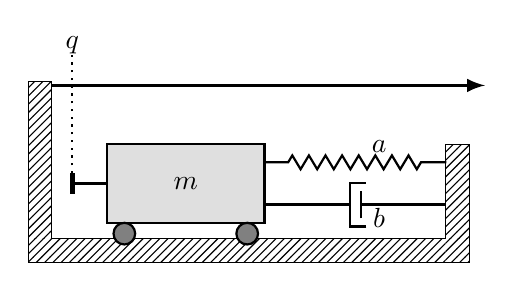
\begin{tikzpicture}[scale=1.1, every node/.style={scale=1}]
\tikzstyle{spring}=[thick,decorate,decoration={zigzag,pre length=0.3cm,post length=0.3cm,segment length=6}]
\tikzstyle{damper}=[thick,decoration={markings,  
  mark connection node=dmp,
  mark=at position 0.5 with 
  {
    \node (dmp) [thick,inner sep=0pt,transform shape,rotate=-90,minimum width=15pt,minimum height=3pt,draw=none] {};
    \draw [thick] ($(dmp.north east)+(2pt,0)$) -- (dmp.south east) -- (dmp.south west) -- ($(dmp.north west)+(2pt,0)$);
    \draw [thick] ($(dmp.north)+(0,-5pt)$) -- ($(dmp.north)+(0,5pt)$);
  }
}, decorate]
\tikzstyle{ground}=[fill,pattern=north east lines,draw=none,minimum width=0.75cm,minimum height=0.3cm,inner sep=0pt,outer sep=0pt]

\node [draw, outer sep=0pt, thick, fill = gray!25] (M) [minimum width=2cm, minimum height=1cm] {$m$};

\node (ground) [ground,anchor=north,yshift=-0.2cm,minimum width=5cm,xshift=0.8cm] at (M.south) {};
\draw (ground.north west) -- (ground.north east);
\draw (ground.south east) -- (ground.south west);

\node (fill) [ground,xshift=-0.15cm,minimum height = 0.3cm, minimum width = 0.3cm] at (ground.west) {};
\draw (fill.north west) -- (fill.south west) -- (fill.south east);

\draw [thick, fill = gray] (M.south west) ++(0.2cm,-0.125cm) circle (0.125cm)  (M.south east) ++(-0.2cm,-0.125cm) circle (0.125cm);

\node (wall) [ground, rotate=-90, minimum width=2cm,anchor=south east] at (fill.north west) {};
\draw (wall.north east) -- (wall.north west) -- (wall.south west) -- (wall.south east);

\node (fill2) [ground,xshift=0.15cm,minimum height = 0.3cm, minimum width = 0.3cm] at (ground.east) {};
\draw (fill2.north east) -- (fill2.south east) -- (fill2.south west);
\node (wall2) [ground, rotate=-90, minimum width=1.2cm,anchor=south east] at (fill2.north west) {};
\draw (wall2.north east) -- (wall2.north west) -- (wall2.south west) -- (wall2.south east);

\draw [-,thick] (M.west) -- +(-0.4cm,0) node [name = t] {};
\draw [-,ultra thick] (t.north) -- (t.south);
\draw [spring] (M.15) -- node [xshift=0.3cm,yshift=0.195cm] {$a$} ++(2.1cm,0cm);
\draw [damper] (M.345) -- node [xshift=0.3cm,yshift=-0.175cm] {$b$} ++(2.1cm,0cm);

\draw [-latex,very thick] (wall.north west) ++(0cm, -0.05cm) -- +(5cm,0cm);
\draw [dotted, thick] (t.north) -- node [yshift=0.85cm] (y1) {$q$} +(0cm,1.4cm);

\end{tikzpicture} 

    \caption[Impact mass--spring--damper system.]{Impact mass--spring--damper system. $q$ is the distance of the cart from the wall, $m$ is the mass of the cart, $a$ is the spring stiffness and $b$ the damping coefficient of the dashpot.} 
    \label{fig:imsd}
\end{figure}
%
\subsubsection{Model of the Flows}
%
When the ball is not touching the floor, the system behaves as a simple damped linear oscillator. Let $\x = [x_1,x_2]^\top = [q,\dot{q}]^\top$. The flows of the system are described by 
\begin{align}
	\dot{\x}&=\begin{bmatrix}x_2\\-ax_1-bx_2\end{bmatrix}
	=\begin{bmatrix}x_2&0&0\\0&-x_1&-x_2\end{bmatrix}\begin{bmatrix}1\\a\\b\end{bmatrix}
\end{align}
%
{where $a$ and $b$ are the spring stiffness and the damping coefficient, respectively}. The corresponding flow set flow set is
%
\begin{equation}
    \C = \{\x:x_1\geq0\}\setminus\{\x:x_1=0,x_2<0\}
\end{equation}
%
\subsubsection{Model of the Jumps}
%
It is clear that during the collision between ball and the floor ($x_1 = q =0$) there is a discontinuity in the velocity. In this example, collisions are considered partially inelastic while the ball is modeled as a rigid body. The selected jump map to model the collisions is the following:
%
\begin{align}
	\x^+=\begin{bmatrix}x_1\\-\lambda x_2+\mu\end{bmatrix} = \begin{bmatrix}x_1&0&0\\0&-x_2&1\end{bmatrix}\begin{bmatrix}1\\\lambda\\\mu\end{bmatrix}
\end{align}
%
{where $\lambda$ is the restitution coefficient and $\mu$ is introduced to consider possible unmodeled impact dynamics}. The jump set is therefore,
%
\begin{equation}
    \D=\{\x:x_1=0,x_2\leq 0\}
\end{equation}
%
\begin{rem}[Hybrid port--Hamiltonian formulation]
    The system indeed belongs to the class of impulsive port--Hamiltonian systems (\ref{eq:impulsive_ph}), defined in Chapter $\ref{chap:HPH_systems}$.
    Let $p\triangleq\dot{q}$. The hybrid port--Hamiltonian formulation of the impact mass--spring--damper system is
    %
    \begin{equation}
        \left\{
            \begin{matrix*}[l]
                \begin{bmatrix}\dot{q}\\\dot{p}\end{bmatrix} = \begin{bmatrix}0&1\\-1&-b\end{bmatrix}\begin{bmatrix}\nabla_q\Ha(q,p)\\\nabla_p\Ha(q,p)\end{bmatrix} + \begin{bmatrix}0\\1\end{bmatrix}u & (q,p)\in\C\\
                \begin{bmatrix}q^+\\{p}^+\end{bmatrix} =\begin{bmatrix}q\\-\lambda p+\mu\end{bmatrix}  & (q,p)\in\D\\
                y = p
            \end{matrix*}
        \right.
    \end{equation}
    %
    with 
    %
    \begin{equation}
        \Ha(q,p) \triangleq \frac{1}{2}p^2 + \frac{a}{2}q^2
    \end{equation}
    %
    Note that, if $\mu\leq 0$, the system is \textit{flow passive}.
\end{rem}
%
\subsubsection{Model Identification}
In order to estimate the system's parameters, a reduced order identification has to be performed for both the flow and the jump as in (\ref{eq:redflow}) and (\ref{eq:redjump}). Let $\bm{\alpha} = \left[{\alpha}_1,{\alpha}_2\right]^\top=\left[a,b\right]^\top$ and $\bm{\beta} = \left[{\beta}_1,{\beta}_2\right]^\top = [\lambda,\mu]^\top$
The reduced model for the flow is
%
\begin{equation}
    \dot{\x}_2 = \begin{bmatrix}-x_1&-x_2\end{bmatrix}\begin{bmatrix}{\alpha}_1\\{\alpha}_2\end{bmatrix}
\end{equation}
%
and the one for the jump is
%
\begin{equation}
    \x_2^+ = \begin{bmatrix}-x_2&1\end{bmatrix}\begin{bmatrix}{\beta}_1\\{\beta}_2\end{bmatrix}
\end{equation}
%
The approximation of the  smoothness bound can be derived by computing the supremum of the norm of the estimated flow map Jacobian. Hence, the estimated flow map in the reduced model will be
%
\begin{equation}
    \hat{{f}}(\x,t)=-\hat{{\alpha}}_1(t)x_1(t)-\hat{{\alpha}}_2(t)x_2(t) = -\bm{\alpha}^\top\x
\end{equation}
%
Therefore,
\begin{align*}
	\frac{\partial \hat{{f}}(\x,t)}{\partial \x} = -\hat{\bm{\alpha}}(t)
	\Rightarrow\sup\limits_{\x\in\hat{\C}}\left\|\frac{\partial \hat{{f}}(\x,t)}{\partial\x}\right\|_2 = \left\|\hat{\bm{\alpha}}(t)\right\|_2
\end{align*}
%
\subsection{Numerical Simulation}
To validate the proposed identification method, numerical simulations have been performed. The simulation experiments have been carried out using Hybrid Equations (HyEQ) Toolbox \cite{sanfelice2013toolbox} for the MATLAB environment. The parameters of the system have been chosen as $a = 5$, $b = 0.1$, $\lambda=0.99$, $\mu=0$. 
%
The initial condition and the time span of the simulation have been set to $\x(t_0)=[20,0]^\top$ and $20$ seconds, respectively. Furthermore, the sampling time $\delta t$ has been chosen to be $0.5\cdot 10^{-3}$ s, the multiplicative constant $r$ in the smoothness bound has been set to 220 and the estimated smoothness bound has been initialized to $10^5$.

Here, as both the flow and jump maps result linear in the state, the chosen estimation scheme is the \textit{recursive least squares} (RLS) \cite{ljung1987system}. However, due to how noise would influence the system, i.e. it affects the observation matrix, alternative results might be achieved with a \textit{recursive generalized total least squares} \citep{RHODE20144637} or a \textit{recursive Frisch scheme} (see [c1,c2]). The resulting time evolution of the system is represented in Fig. \ref{fig:trj}. 
\begin{figure}
	\centering
%	\includegraphics[trim={15 0 0 0},scale=.58]{trj}
    % This file was created by matlab2tikz.
%
%The latest updates can be retrieved from
%  http://www.mathworks.com/matlabcentral/fileexchange/22022-matlab2tikz-matlab2tikz
%where you can also make suggestions and rate matlab2tikz.
%
\definecolor{mycolor1}{rgb}{0.00000,0.44700,0.74100}%
%
\begin{tikzpicture}
%\footnotesize

\begin{axis}[%
width=9cm,
height=2.5cm,
at={(0.86in,2.2in)},
scale only axis,
xmin=0,
xmax=20,
ymin=-2.665645482125e-12,
ymax=20,
ylabel style={font=\color{white!15!black}},
ylabel={$x_1(t) = q(t)$},
axis background/.style={fill=white},
legend style={legend cell align=left, align=left, draw=white!15!black}
]
\addplot [color=black, line width=1.5pt]
  table[row sep=crcr]{%
0	20\\
0	20\\
0.000126191468896039	19.999999203789\\
0.000252382937792077	19.9999968151695\\
0.000378574406688116	19.9999928341618\\
0.000504765875584155	19.9999872607862\\
0.00113572322006435	19.9999355091145\\
0.00176668056454454	19.9998439513818\\
0.00239763790902473	19.9997125902819\\
0.00302859525350493	19.9995414285877\\
0.00618338197590589	19.9980887137718\\
0.00933816869830686	19.9956414454642\\
0.0124929554207078	19.992200059144\\
0.0156477421431088	19.9877650395981\\
0.0276481601076166	19.9618263167084\\
0.0396485780721244	19.9215546749277\\
0.0516489960366322	19.866996276571\\
0.06364941400114	19.7982075093252\\
0.0795171060289317	19.6855171395325\\
0.0953847980567235	19.5482452791905\\
0.111252490084515	19.3866035496145\\
0.127120182112307	19.2008338295377\\
0.145352130059267	18.95795008083\\
0.163584078006226	18.6840334854967\\
0.181816025953186	18.3795953849762\\
0.200047973900146	18.0451965342848\\
0.220071234980976	17.6441482118668\\
0.240094496061806	17.2085733293003\\
0.260117757142636	16.7394132942873\\
0.280141018223465	16.237673951143\\
0.301708193087325	15.6620310918154\\
0.323275367951185	15.0512499408405\\
0.344842542815045	14.4068253719306\\
0.366409717678905	13.7303252164943\\
0.389458650570211	12.973744025447\\
0.412507583461517	12.1844913788867\\
0.435556516352823	11.3647370424498\\
0.458605449244129	10.5167230979711\\
0.481800361400667	9.63714868602161\\
0.504995273557205	8.73372514967301\\
0.528190185713743	7.80893592384127\\
0.551385097870281	6.86531151233252\\
0.572725339283812	5.9827171210837\\
0.594065580697343	5.0883994583547\\
0.615405822110874	4.1844184005378\\
0.636746063524405	3.27284792754387\\
0.655724669033981	2.45746986002715\\
0.674703274543557	1.63921747342536\\
0.693681880053134	0.819568951208989\\
0.71266048556271	-1.16795462190566e-13\\
};
%egendentry{data1}

\addplot [color=black, line width=1.5pt]
  table[row sep=crcr]{%
0.71266048556271	-1.16795462190566e-13\\
0.71266048556271	-1.16795462190566e-13\\
0.712955847869028	0.0126189596129195\\
0.713251210175347	0.0252375410107193\\
0.713546572481665	0.0378557387003791\\
0.713841934787984	0.0504735471893269\\
0.715318746319577	0.113556559409491\\
0.716795557851169	0.176629017917934\\
0.718272369382762	0.23969023652624\\
0.719749180914355	0.302739529275859\\
0.727133238572319	0.61778312183889\\
0.734517296230282	0.932425810234085\\
0.741901353888246	1.24658213969462\\
0.74928541154621	1.56016686985453\\
0.763502620608957	2.16201786746632\\
0.777719829671705	2.76083038101713\\
0.791937038734452	3.35600386151082\\
0.8061542477972	3.94694278678755\\
0.823290826869658	4.65275954696095\\
0.840427405942117	5.35054247500561\\
0.857563985014576	6.03928135536863\\
0.874700564087035	6.71798222602084\\
0.893860482784055	7.46373027842436\\
0.913020401481075	8.19436575900548\\
0.932180320178095	8.90857727943182\\
0.951340238875115	9.60508820806833\\
0.972141894914274	10.3397948501332\\
0.992943550953433	11.0506307160876\\
1.01374520699259	11.7361083120558\\
1.03454686303175	12.3948010671445\\
1.05684159758016	13.0694840401591\\
1.07913633212858	13.7102252456922\\
1.10143106667699	14.3155085611607\\
1.12372580122541	14.8839131350341\\
1.14740771745168	15.4458111627729\\
1.17108963367795	15.96312788429\\
1.19477154990422	16.4345184665667\\
1.21845346613049	16.858774356195\\
1.24035979590319	17.2083202759852\\
1.26226612567589	17.5158640540576\\
1.28417245544859	17.7807597207985\\
1.30607878522129	18.0024671767266\\
1.32593990787618	18.1657806399565\\
1.34580103053108	18.2929826286987\\
1.36566215318598	18.3838938163702\\
1.38552327584088	18.4384075932583\\
1.40289087903558	18.4562184192618\\
1.42025848223028	18.4461909090966\\
1.43762608542497	18.4083883711415\\
1.45499368861967	18.3429160315414\\
1.47007626831375	18.2637219725677\\
1.48515884800783	18.1638913797042\\
1.50024142770191	18.0435687955398\\
1.51532400739599	17.9029218056077\\
1.53303076113948	17.7121261385877\\
1.55073751488298	17.4939299726845\\
1.56844426862648	17.2487235048843\\
1.58615102236997	16.9769383256841\\
1.60575291074699	16.6456381807801\\
1.62535479912401	16.2830444129758\\
1.64495668750104	15.8899142399392\\
1.66455857587806	15.4670613128123\\
1.68574693571507	14.9775614103505\\
1.70693529555209	14.4555193598167\\
1.72812365538911	13.9021747809028\\
1.74931201522613	13.3188333200789\\
1.77198263544398	12.6630191231148\\
1.79465325566183	11.9761935150489\\
1.81732387587968	11.2601900901953\\
1.83999449609754	10.51691029426\\
1.86363936925682	9.71475515600215\\
1.8872842424161	8.88737755918985\\
1.91092911557539	8.03714789951455\\
1.93457398873467	7.16649034677414\\
1.95640703129971	6.34655047407202\\
1.97824007386476	5.51329289591894\\
2.0000731164298	4.66873114009761\\
2.02190615899484	3.81489774912013\\
2.04168484028799	3.03511556783754\\
2.06146352158114	2.25094501071307\\
2.08124220287429	1.46392753245248\\
2.10102088416744	0.675604766545745\\
2.1052593564867	0.506649350587227\\
2.10949782880595	0.337719947961567\\
2.11373630112521	0.168831768713831\\
2.11797477344446	-4.82169859594705e-13\\
};
%%egendentry{data2}

\addplot [color=mycolor1, dotted, line width=1.0pt, mark size=1.5pt, mark=asterisk, mark options={solid, fill=gray, gray}]
  table[row sep=crcr]{%
0.71266048556271	-1.16795462190566e-13\\
0.71266048556271	-1.16795462190566e-13\\
};
%%egendentry{data3}

\addplot [color=black, line width=1.5pt]
  table[row sep=crcr]{%
2.11797477344446	-4.82169859594705e-13\\
2.11797477344446	-4.82169859594705e-13\\
2.11829483681149	0.0126189438676957\\
2.11861490017851	0.0252374773928329\\
2.11893496354553	0.0378555941248824\\
2.11925502691256	0.0504732876142727\\
2.12085534374767	0.113555180719346\\
2.12245566058279	0.176625525564236\\
2.12405597741791	0.239683516439594\\
2.12565629425302	0.302728347931474\\
2.1336578784286	0.617726958449652\\
2.14165946260418	0.932275947496817\\
2.14966104677976	1.24627501393359\\
2.15766263095534	1.55962413873017\\
2.17210867042261	2.12337793240863\\
2.18655470988987	2.68410395597894\\
2.20100074935714	3.2412218095027\\
2.2154467888244	3.79415619120717\\
2.23272736833193	4.44929241107515\\
2.25000794783947	5.09666054369097\\
2.267288527347	5.73530798034574\\
2.28456910685454	6.36429797353247\\
2.30383919311945	7.0531874106365\\
2.32310927938437	7.72766924076261\\
2.34237936564929	8.3865196245531\\
2.36164945191421	9.02854808964311\\
2.38254650666801	9.70442718987452\\
2.40344356142182	10.3577316893883\\
2.42434061617562	10.9870830275905\\
2.44523767092943	11.5911606095607\\
2.46762420449579	12.2088220852721\\
2.49001073806216	12.7945494794438\\
2.51239727162852	13.3469471350779\\
2.53478380519489	13.8647095567399\\
2.55835704859259	14.3711445958366\\
2.58193029199029	14.8365125733303\\
2.605503535388	15.2596174719699\\
2.6290767787857	15.6393873492776\\
2.65086589188565	15.9510499404283\\
2.6726550049856	16.2242174850569\\
2.69444411808555	16.4583253530246\\
2.7162332311855	16.6529047294774\\
2.73596748835466	16.7947067725888\\
2.75570174552381	16.9035639683676\\
2.77543600269296	16.9793292090018\\
2.79517025986212	17.021920787247\\
2.81236092130652	17.0319722525132\\
2.82955158275092	17.0168648274309\\
2.84674224419532	16.9766639367958\\
2.86393290563973	16.9114720789629\\
2.87922900288253	16.8325654993826\\
2.89452510012534	16.7341048964339\\
2.90982119736815	16.6162352312511\\
2.92511729461096	16.4791238986312\\
2.94296722918862	16.2950460002234\\
2.96081716376628	16.0853634408954\\
2.97866709834395	15.8504556056461\\
2.99651703292161	15.5907411291298\\
3.01623241430944	15.2756050051674\\
3.03594779569726	14.9314360295398\\
3.05566317708508	14.5589596304773\\
3.07537855847291	14.1589540890403\\
3.09666795646215	13.6970577871726\\
3.1179573544514	13.2051430042799\\
3.13924675244064	12.684387304839\\
3.16053615042989	12.1360295489024\\
3.18330666981761	11.5204444463421\\
3.20607718920533	10.8764342161001\\
3.22884770859305	10.2057315609182\\
3.25161822798078	9.51013158989316\\
3.27514370847273	8.76729041346104\\
3.29866918896469	8.00196885247963\\
3.32219466945665	7.21633572663269\\
3.34572014994861	6.41260685692784\\
3.36742412118392	5.65701299033144\\
3.38912809241923	4.8897512078299\\
3.41083206365454	4.11265258341808\\
3.43253603488985	3.32756419890733\\
3.45217379031709	2.61188482538239\\
3.47181154574433	1.89257956998755\\
3.49144930117157	1.17104158251362\\
3.51108705659881	0.448663490638958\\
3.5141375591335	0.336464603605832\\
3.5171880616682	0.224284239220132\\
3.52023856420289	0.112127629383403\\
3.52328906673759	-3.96016552883793e-13\\
};
%%egendentry{data4}

\addplot [color=mycolor1, dotted, line width=1.0pt, mark size=1.5pt, mark=asterisk, mark options={solid, fill=gray, gray}]
  table[row sep=crcr]{%
2.11797477344446	-4.82169859594705e-13\\
2.11797477344446	-4.82169859594705e-13\\
};
%%egendentry{data5}

\addplot [color=black, line width=1.5pt]
  table[row sep=crcr]{%
3.52328906673759	-3.96016552883793e-13\\
3.52328906673759	-3.96016552883793e-13\\
3.5236358969078	0.0126189267917385\\
3.52398272707801	0.0252374083394138\\
3.52432955724823	0.0378554370687596\\
3.52467638741844	0.0504730054063961\\
3.52641053826951	0.113553676195286\\
3.52814468912058	0.176621701501812\\
3.52987883997164	0.239676135282758\\
3.53161299082271	0.302716031874665\\
3.54028374507805	0.617664402776339\\
3.54895449933339	0.932107720218401\\
3.55762525358872	1.24592826321028\\
3.56629600784406	1.55900868254307\\
3.58097438776973	2.08699546246245\\
3.59565276769541	2.6119612655599\\
3.61033114762108	3.13334529646683\\
3.62500952754675	3.6505919358197\\
3.64243895355396	4.25864973450544\\
3.65986837956118	4.85918623300984\\
3.67729780556839	5.45130288842576\\
3.69472723157561	6.03411666155787\\
3.71411224299136	6.67033896614796\\
3.73349725440711	7.29280991655066\\
3.75288226582286	7.90038725949764\\
3.77226727723862	8.49196082121752\\
3.79326454803279	9.11343117156367\\
3.81426181882696	9.71353220481969\\
3.83525908962113	10.2909865656314\\
3.8562563604153	10.8445721205768\\
3.87873997832658	11.409558589341\\
3.90122359623787	11.9444754847071\\
3.92370721414915	12.4480388775823\\
3.94619083206043	12.9190502630116\\
3.96964932183274	13.3745814015142\\
3.99310781160505	13.7922958010649\\
4.01656630137735	14.1711329917699\\
4.04002479114966	14.5101453521836\\
4.06168911755179	14.7871310853299\\
4.08335344395393	15.0288602330993\\
4.10501777035606	15.23484184749\\
4.1266820967582	15.4046715629601\\
4.14627947971066	15.5268878825378\\
4.16587686266311	15.6190827169247\\
4.18547424561556	15.681137714725\\
4.20507162856802	15.7129932083193\\
4.22206708663967	15.7161651917171\\
4.23906254471133	15.6966560746724\\
4.25605800278298	15.6545324474565\\
4.27305346085463	15.5898935296123\\
4.28856186457498	15.5113747436655\\
4.30407026829533	15.4143407380624\\
4.31957867201568	15.2989367810636\\
4.33508707573603	15.1653299527303\\
4.35308139749662	14.9877433735194\\
4.37107571925721	14.7862364293221\\
4.38907004101779	14.561178043716\\
4.40706436277838	14.3129743447791\\
4.42689521441243	14.0131607524268\\
4.44672606604647	13.6864189285998\\
4.46655691768052	13.3334440834268\\
4.48638776931456	12.9549809141127\\
4.50778071151252	12.5190407234675\\
4.52917365371049	12.0554215132384\\
4.55056659590845	11.5652423323584\\
4.57195953810642	11.0496791092677\\
4.5948331849831	10.4717456404966\\
4.61770683185979	9.86777643496879\\
4.64058047873648	9.23940952299365\\
4.66345412561316	8.58834028252946\\
4.68685679558895	7.90054338466397\\
4.71025946556474	7.19275050827037\\
4.73366213554053	6.46694497158074\\
4.75706480551632	5.72515104053702\\
4.77863476906376	5.02906847762742\\
4.8002047326112	4.32280221465356\\
4.82177469615864	3.60801596389712\\
4.84334465970608	2.88638679731664\\
4.8628339335124	2.22988931481852\\
4.88232320731872	1.57044043751848\\
4.90181248112504	0.909297473491976\\
4.92130175493136	0.247716633456946\\
4.92312715748719	0.185774150051324\\
4.92495256004302	0.123839860604262\\
4.92677796259885	0.061914799406462\\
4.92860336515468	-9.26092535991074e-13\\
};
%%egendentry{data6}

\addplot [color=mycolor1, dotted, line width=1.0pt, mark size=1.5pt, mark=asterisk, mark options={solid, fill=gray, gray}]
  table[row sep=crcr]{%
3.52328906673759	-3.96016552883793e-13\\
3.52328906673759	-3.96016552883793e-13\\
};
%egendentry{data7}

\addplot [color=black, line width=1.5pt]
  table[row sep=crcr]{%
4.92860336515468	-9.26092535991074e-13\\
4.92860336515468	-9.26092535991074e-13\\
4.9289792006279	0.0126189082701147\\
4.92935503610111	0.0252373333746489\\
4.92973087157433	0.0378552664191234\\
4.93010670704755	0.0504726985105827\\
4.93198588441363	0.113552033477525\\
4.93386506177972	0.176617511083581\\
4.93574423914581	0.239668020515936\\
4.93762341651189	0.30270245145043\\
4.94701930334232	0.617594625536573\\
4.95641519017275	0.931918579754986\\
4.96581107700317	1.24553615558805\\
4.9752069638336	1.55830968524845\\
4.99012122072234	2.05271097684226\\
5.00503547761108	2.54409426328169\\
5.01994973449982	3.03191783598461\\
5.03486399138857	3.51564524702369\\
5.05244728514176	4.07995625159521\\
5.07003057889495	4.63697490469765\\
5.08761387264814	5.18585344398046\\
5.10519716640133	5.72575928669275\\
5.12470210627837	6.31318301027547\\
5.1442070461554	6.88746621856667\\
5.16371198603244	7.44754273367683\\
5.18321692590948	7.99237726574151\\
5.2043195434863	8.5635130900224\\
5.22542216106313	9.11440044073624\\
5.24652477863996	9.6438560391903\\
5.26762739621679	10.1507492843005\\
5.29021379856798	10.667064712082\\
5.31280020091917	11.1550422761701\\
5.33538660327036	11.6135017295155\\
5.35797300562156	12.041343858442\\
5.38131019127706	12.4501656429229\\
5.40464737693256	12.8241777262563\\
5.42798456258807	13.1624429945616\\
5.45132174824357	13.4641268567077\\
5.47285298807291	13.7093848915645\\
5.49438422790224	13.9223775036371\\
5.51591546773158	14.1026803903002\\
5.53744670756091	14.2499473543859\\
5.5568959930249	14.3543502371802\\
5.57634527848889	14.4314314100667\\
5.59579456395287	14.4810980867813\\
5.61524384941686	14.5033099989796\\
5.63202269472414	14.5004206130677\\
5.64880154003142	14.4771440932203\\
5.66558038533871	14.4335472928274\\
5.68235923064599	14.3697256165022\\
5.69807878214861	14.2916927475299\\
5.71379833365122	14.1961404709004\\
5.72951788515384	14.0832142478833\\
5.74523743665645	13.9530807197231\\
5.76337730967885	13.7817714760808\\
5.78151718270124	13.588121664794\\
5.79965705572364	13.3724900732718\\
5.81779692874603	13.1352707419293\\
5.83774522635693	12.8499914367397\\
5.85769352396784	12.5397433341937\\
5.87764182157874	12.2051928954121\\
5.89759011918964	11.8470529038376\\
5.91908915909488	11.4355320961451\\
5.94058819900012	10.9985009989563\\
5.96208723890536	10.5370234486802\\
5.98358627881059	10.0522160383803\\
6.00656639932362	9.50953593255843\\
6.02954651983665	8.94302736876291\\
6.05252664034968	8.35423949855715\\
6.07550676086271	7.74477412071867\\
6.09878308889206	7.10806606183099\\
6.12205941692141	6.45361072062487\\
6.14533574495077	5.78322073392098\\
6.16861207298012	5.09874428495029\\
6.19004280375584	4.45770513919677\\
6.21147353453155	3.80781536421975\\
6.23290426530726	3.15058519478485\\
6.25433499608298	2.48753590116795\\
6.27366758997621	1.88567992491412\\
6.29300018386944	1.28146691310493\\
6.31233277776267	0.676029790047115\\
6.33166537165591	0.0704999197125549\\
6.33222844548612	0.0528735513519476\\
6.33279151931634	0.0352480899428688\\
6.33335459314656	0.0176235634919423\\
6.33391766697677	-8.93979335003792e-13\\
};
%egendentry{data8}

\addplot [color=mycolor1, dotted, line width=1.0pt, mark size=1.5pt, mark=asterisk, mark options={solid, fill=gray, gray}]
  table[row sep=crcr]{%
4.92860336515468	-9.26092535991074e-13\\
4.92860336515468	-9.26092535991074e-13\\
};
%egendentry{data9}

\addplot [color=black, line width=1.5pt]
  table[row sep=crcr]{%
6.33391766697677	-8.93979335003792e-13\\
6.33391766697677	-8.93979335003792e-13\\
6.33432493345776	0.0126188881802234\\
6.33473219993875	0.0252372519817777\\
6.33513946641973	0.0378550809605497\\
6.33554673290072	0.0504723646741957\\
6.33758306530566	0.113550238855372\\
6.3396193977106	0.176612915564935\\
6.34165573011553	0.239659090531774\\
6.34369206252047	0.302687460114063\\
6.35387372454516	0.617516676978909\\
6.36405538656984	0.931705588885767\\
6.37423704859453	1.24509206187558\\
6.38441871061922	1.55751461075209\\
6.39957240273415	2.02037218693783\\
6.41472609484909	2.4802110078725\\
6.42987978696403	2.93650796091112\\
6.44503347907897	3.38874528582663\\
6.46277584312659	3.91239055595119\\
6.48051820717421	4.4289556342156\\
6.49826057122183	4.93764049271073\\
6.51600293526945	5.43765999106385\\
6.53563306776776	5.97985508028782\\
6.55526320026607	6.50947815055058\\
6.57489333276438	7.02553400881942\\
6.59452346526269	7.52705724892007\\
6.6157369003489	8.05161442260124\\
6.6369503354351	8.55696551547314\\
6.65816377052131	9.04201475287961\\
6.67937720560751	9.50571667979348\\
6.70207255169003	9.97704875947126\\
6.72476789777255	10.4216515014264\\
6.74746324385507	10.8384409361006\\
6.77015858993759	11.2264100597916\\
6.79336739968306	11.5923817182095\\
6.81657620942853	11.9263265078764\\
6.83978501917399	12.2274194678291\\
6.86299382891946	12.4949286630068\\
6.8843828472113	12.7111719787993\\
6.90577186550315	12.8979134627509\\
6.92716088379499	13.0547889883354\\
6.94854990208684	13.1815047523169\\
6.96783843153271	13.2697265367817\\
6.98712696097857	13.3331210397884\\
7.00641549042444	13.3716180940145\\
7.02570401987031	13.3851943903655\\
7.04224083221757	13.3770085784198\\
7.05877764456483	13.3505627020024\\
7.07531445691209	13.3059230118155\\
7.09185126925935	13.2431805667057\\
7.10778075032975	13.1657325075553\\
7.12371023140015	13.0717188983883\\
7.13963971247055	12.961285270171\\
7.15556919354095	12.8345976939764\\
7.17385565094375	12.669367755466\\
7.19214210834654	12.4832792612219\\
7.21042856574933	12.2766811530528\\
7.22871502315213	12.049955762714\\
7.24878266872	11.7784770150733\\
7.26885031428787	11.4838539355373\\
7.28891795985574	11.1667255953582\\
7.30898560542361	10.8277744111073\\
7.3305932802434	10.4392443463397\\
7.3522009550632	10.0272144193401\\
7.373808629883	9.59269631889281\\
7.39541630470279	9.13675064038257\\
7.41850630384074	8.62709700298682\\
7.4415963029787	8.09565359879195\\
7.46468630211664	7.54388607781625\\
7.48777630125459	6.97330836937923\\
7.51092271193675	6.38402512434141\\
7.53406912261891	5.77902735751608\\
7.55721553330106	5.15997069828939\\
7.58036194398322	4.52854151354541\\
7.60164798415328	3.93841565706798\\
7.62293402432334	3.34063403411202\\
7.64422006449341	2.7365661883684\\
7.66550610466347	2.12759066774554\\
7.68393757071615	1.59738776920095\\
7.70236903676882	1.06545110124097\\
7.7208005028215	0.532686960680167\\
7.73923196887418	-1.63735691671718e-12\\
};
%egendentry{data10}

\addplot [color=mycolor1, dotted, line width=1.0pt, mark size=1.5pt, mark=asterisk, mark options={solid, fill=gray, gray}]
  table[row sep=crcr]{%
6.33391766697677	-8.93979335003792e-13\\
6.33391766697677	-8.93979335003792e-13\\
};
%egendentry{data11}

\addplot [color=black, line width=1.5pt]
  table[row sep=crcr]{%
7.73923196887418	-1.63735691671718e-12\\
7.73923196887418	-1.63735691671718e-12\\
7.73967329492841	0.0126188663860073\\
7.74011462098264	0.0252371635939842\\
7.74055594703687	0.0378548793594101\\
7.7409972730911	0.0504720014205189\\
7.74320390336225	0.11354827709355\\
7.74541053363341	0.176607871546671\\
7.74761716390456	0.23964925336921\\
7.74982379417571	0.302670891961625\\
7.76085694553148	0.617429467972605\\
7.77189009688724	0.93146535908037\\
7.78292324824301	1.2445883088883\\
7.79395639959877	1.55660892004927\\
7.80935310126931	1.98983312866864\\
7.82474980293986	2.42003421233062\\
7.8401465046104	2.84670719075871\\
7.85554320628095	3.26935253527239\\
7.87345003191049	3.75518098507058\\
7.89135685754004	4.2341255979386\\
7.90926368316959	4.70543125798542\\
7.92717050879914	5.16835747563211\\
7.94693137618627	5.66861773121001\\
7.96669224357339	6.1568349827149\\
7.98645311096052	6.63208032211862\\
8.00621397834765	7.09345361210811\\
8.02754407211553	7.5748938515631\\
8.04887416588341	8.0380975129009\\
8.07020425965129	8.48205026875875\\
8.09153435341917	8.90578592769869\\
8.11434531347791	9.33553027730174\\
8.13715627353664	9.74003953634054\\
8.15996723359538	10.1183192031394\\
8.18277819365412	10.4694479760665\\
8.20585097361927	10.7961203695102\\
8.22892375358443	11.093342165753\\
8.25199653354959	11.3603902601012\\
8.27506931351474	11.5966258396195\\
8.29630601205202	11.7863507648621\\
8.3175427105893	11.9491281288288\\
8.33877940912659	12.0846480302433\\
8.36001610766387	12.1926637475944\\
8.37912950793115	12.2662094003284\\
8.39824290819844	12.3172337909908\\
8.41735630846573	12.3456866457487\\
8.43646970873302	12.3515593541817\\
8.45273383765996	12.3387979271766\\
8.46899796658691	12.309752898281\\
8.48526209551386	12.2644890731556\\
8.50152622444081	12.2030926283311\\
8.51766420952741	12.1263327509436\\
8.53380219461401	12.0339205466777\\
8.54994017970061	11.9260014752455\\
8.56607816478721	11.8027408897625\\
8.58451198547023	11.6434123438314\\
8.60294580615325	11.4646158628166\\
8.62137962683627	11.2666907870835\\
8.63981344751929	11.0500080668928\\
8.66000216536213	10.7916527363078\\
8.68019088320497	10.51185207292\\
8.70037960104781	10.2112189966443\\
8.72056831889065	9.89040697083338\\
8.74228705422081	9.52354546165765\\
8.76400578955097	9.13504763811392\\
8.78572452488113	8.72587586276256\\
8.8074432602113	8.29703780856456\\
8.83064650828568	7.81834864565842\\
8.85384975636006	7.31975212687814\\
8.87705300443445	6.80263536495392\\
8.90025625250883	6.26842969308948\\
8.92326923507608	5.72317713195879\\
8.94628221764333	5.16404459457252\\
8.96929520021058	4.59254333377122\\
8.99230818277783	4.01021106981466\\
9.01344394324107	3.46717855942765\\
9.03457970370431	2.91755847673569\\
9.05571546416754	2.36259146798807\\
9.07685122463078	1.80352541749457\\
9.09377498553109	1.35376091496968\\
9.11069874643141	0.90282030011926\\
9.12762250733172	0.451351235726211\\
9.14454626823203	-1.19282361765727e-12\\
};
%egendentry{data12}

\addplot [color=mycolor1, dotted, line width=1.0pt, mark size=1.5pt, mark=asterisk, mark options={solid, fill=gray, gray}]
  table[row sep=crcr]{%
7.73923196887418	-1.63735691671718e-12\\
7.73923196887418	-1.63735691671718e-12\\
};
%egendentry{data13}

\addplot [color=black, line width=1.5pt]
  table[row sep=crcr]{%
9.14454626823203	-1.19282361765727e-12\\
9.14454626823203	-1.19282361765727e-12\\
9.14502450225007	0.0126188427429212\\
9.1455027362681	0.0252370675956838\\
9.14598097028614	0.0378546601576024\\
9.14645920430418	0.0504716060304687\\
9.14885037439436	0.113546131245613\\
9.15124154448455	0.176602330346262\\
9.15363271457473	0.239638405240608\\
9.15602388466491	0.302652558882972\\
9.16797973511584	0.617331748015778\\
9.17993558556676	0.931193977379532\\
9.19189143601768	1.24401600833781\\
9.2038472864686	1.55557574155387\\
9.21949058122067	1.96095328316728\\
9.23513387597273	2.36329981668567\\
9.25077717072479	2.76212805838302\\
9.26642046547686	3.15695628301819\\
9.28449734185441	3.6076017100036\\
9.30257421823196	4.05154477503545\\
9.32065109460951	4.48807266122794\\
9.33872797098706	4.9164869465261\\
9.35862541354478	5.37785075591901\\
9.37852285610249	5.82766376114734\\
9.39842029866021	6.26505900278544\\
9.41831774121792	6.68919735613272\\
9.43977074050149	7.1307105326865\\
9.46122373978505	7.55488890699423\\
9.48267673906862	7.9607940212566\\
9.50412973835218	8.34753353304832\\
9.52706355435525	8.73881599754723\\
9.54999737035832	9.10625158530424\\
9.57293118636139	9.44892900538242\\
9.59586500236446	9.76600668300588\\
9.61879344437575	10.0566471763067\\
9.64172188638703	10.3202231066649\\
9.66465032839831	10.5561037600646\\
9.6875787704096	10.7637346818444\\
9.7086519298906	10.9292389724528\\
9.72972508937161	11.0701575523685\\
9.75079824885261	11.1862292677287\\
9.77187140833361	11.2772495877668\\
9.79079323240813	11.3375085271953\\
9.80971505648264	11.3773795840404\\
9.82863688055716	11.3968298502228\\
9.84755870463167	11.3958633130311\\
9.86351248400004	11.379212999512\\
9.87946626336841	11.3481209566103\\
9.89542004273677	11.3026497109837\\
9.91137382210514	11.2428800012857\\
9.92771846982128	11.1669211082605\\
9.94406311753742	11.0761840655504\\
9.96040776525356	10.9708140914089\\
9.9767524129697	10.8509756443635\\
9.9953339421764	10.6973961477788\\
10.0139154713831	10.5256540422209\\
10.0324970005898	10.336079248523\\
10.0510785297965	10.1290315946832\\
10.0713897113403	9.88318266465353\\
10.0917008928841	9.6174707501039\\
10.1120120744279	9.33248372173843\\
10.1323232559716	9.0288473548792\\
10.1541552190143	8.68243872188252\\
10.175987182057	8.31612088391316\\
10.1978191450997	7.93080944327198\\
10.2196511081424	7.52746195284115\\
10.2429707902342	7.07783564619821\\
10.2662904723259	6.61003921008712\\
10.2896101544176	6.12538576619191\\
10.3129298365093	5.62522888588981\\
10.3358061179467	5.12086239492697\\
10.358682399384	4.60426799631543\\
10.3815586808213	4.07682425399847\\
10.4044349622587	3.53993242052909\\
10.4254149027067	3.0404569172304\\
10.4463948431547	2.53534556247224\\
10.4673747836027	2.02572100861802\\
10.4883547240508	1.51271162043549\\
10.5037311837978	1.13522681552839\\
10.5191076435449	0.756981183123282\\
10.5344841032919	0.378423131103126\\
10.549860563039	-2.665645482125e-12\\
};
%egendentry{data14}

\addplot [color=mycolor1, dotted, line width=1.0pt, mark size=1.5pt, mark=asterisk, mark options={solid, fill=gray, gray}]
  table[row sep=crcr]{%
9.14454626823203	-1.19282361765727e-12\\
9.14454626823203	-1.19282361765727e-12\\
};
%egendentry{data15}

\addplot [color=black, line width=1.5pt]
  table[row sep=crcr]{%
10.549860563039	-2.665645482125e-12\\
10.549860563039	-2.665645482125e-12\\
10.5503787916208	0.0126188170883598\\
10.5508970202026	0.0252369633089951\\
10.5514152487844	0.0378544217507398\\
10.5519334773663	0.0504711755069113\\
10.5545246202753	0.113543782425268\\
10.5571157631844	0.176596237259052\\
10.5597069060935	0.239626428813967\\
10.5622980490026	0.302632247246677\\
10.575253763548	0.617222079617941\\
10.5882094780934	0.930886921117079\\
10.6011651926388	1.24336485726238\\
10.6141209071842	1.55439548692878\\
10.6300143794789	1.93359667371086\\
10.6459078517736	2.30975556803617\\
10.6618013240683	2.68240217526661\\
10.677694796363	3.05107217413241\\
10.6959475218566	3.46896899474653\\
10.7142002473502	3.88033091840745\\
10.7324529728439	4.28448501044285\\
10.7507056983375	4.68077252828627\\
10.7707458775613	5.10604200022799\\
10.790786056785	5.52021853931838\\
10.8108262360087	5.922493136715\\
10.8308664152325	6.31208375798197\\
10.8524490135885	6.71660847758712\\
10.8740316119446	7.10463723868529\\
10.8956142103006	7.47530232045109\\
10.9171968086566	7.82778024980786\\
10.9402613662397	8.18347744808214\\
10.9633259238228	8.51661758218884\\
10.9863904814059	8.82636682843337\\
11.009455038989	9.11195785923574\\
11.0322300939025	9.36957328583222\\
11.055005148816	9.60233505491379\\
11.0777802037294	9.80969613906603\\
11.1005552586429	9.99117838337985\\
11.1214523419266	10.1345779915292\\
11.1423494252102	10.2555769872007\\
11.1632465084938	10.3539579169648\\
11.1841435917774	10.4295539329365\\
11.2028548485766	10.477811246214\\
11.2215661053758	10.5076561526622\\
11.240277362175	10.5190707579398\\
11.2589886189742	10.5120696865959\\
11.2745846357869	10.4921951829698\\
11.2901806525997	10.4596025144982\\
11.3057766694125	10.4143510847298\\
11.3213726862252	10.3565156026734\\
11.3379214254444	10.2814870093985\\
11.3544701646636	10.1925172783767\\
11.3710189038828	10.0897511699671\\
11.387567643102	9.97335202466583\\
11.4062965178745	9.82540260388716\\
11.425025392647	9.66051644220057\\
11.4437542674195	9.47901413755991\\
11.4624831421919	9.2812445635792\\
11.4829176040447	9.04735127611459\\
11.5033520658975	8.79506885266768\\
11.5237865277504	8.52496105565323\\
11.5442209896032	8.23762706478766\\
11.5661678551672	7.91056502460062\\
11.5881147207313	7.56519390277994\\
11.6100615862954	7.20238482876065\\
11.6320084518595	6.82304774315499\\
11.6554473196423	6.40074156471068\\
11.6788861874252	5.96186713464117\\
11.7023250552081	5.50766769250827\\
11.725763922991	5.03942342642653\\
11.7485007518135	4.57302844723956\\
11.771237580636	4.09588888866041\\
11.7939744094585	3.60926147044707\\
11.8167112382811	3.11442227170391\\
11.8375301866005	2.65522471047941\\
11.8583491349199	2.1912353878333\\
11.8791680832393	1.72346908083434\\
11.8999870315587	1.25294497211844\\
11.9137839867051	0.940104077563774\\
11.9275809418516	0.626800408397559\\
11.9413778969981	0.3133329675529\\
11.9551748521446	-9.34807786734382e-13\\
};
%egendentry{data16}

\addplot [color=mycolor1, dotted, line width=1.0pt, mark size=1.5pt, mark=asterisk, mark options={solid, fill=gray, gray}]
  table[row sep=crcr]{%
10.549860563039	-2.665645482125e-12\\
10.549860563039	-2.665645482125e-12\\
};
%egendentry{data17}

\addplot [color=black, line width=1.5pt]
  table[row sep=crcr]{%
11.9551748521446	-9.34807786734382e-13\\
11.9551748521446	-9.34807786734382e-13\\
11.9557364200216	0.0126187892537565\\
11.9562979878986	0.025236850000979\\
11.9568595557756	0.0378541623861732\\
11.9574211236526	0.0504707065570996\\
11.9602289630377	0.113541209567794\\
11.9630368024228	0.176589530729227\\
11.9658446418079	0.239613191248562\\
11.968652481193	0.302609714078937\\
11.9826916781184	0.617098808501141\\
11.9967308750438	0.930538958524725\\
12.0107700719692	1.24262290540783\\
12.0248092688946	1.55304540376875\\
12.0409564942093	1.90763093132039\\
12.0571037195239	2.2591596014029\\
12.0732509448386	2.60717833010521\\
12.0893981701533	2.95123983002801\\
12.1078327664147	3.33863761716436\\
12.126267362676	3.71965478237371\\
12.1447019589374	4.09365604046951\\
12.1631365551988	4.46002012352001\\
12.1833259810842	4.85177874634941\\
12.2035154069696	5.23287029899263\\
12.223704832855	5.60254004049841\\
12.2438942587404	5.96005941556149\\
12.2656136447323	6.33030199781369\\
12.2873330307242	6.68482898592447\\
12.3090524167161	7.02283867752556\\
12.3307718027079	7.3435718939164\\
12.353975717082	7.66633014426174\\
12.3771796314561	7.96772980217477\\
12.4003835458302	8.24700924600956\\
12.4235874602042	8.50347037754292\\
12.4461992328756	8.73082826653846\\
12.468811005547	8.93538226650682\\
12.4914227782184	9.1166610298517\\
12.5140345508898	9.27425528840076\\
12.5347414544284	9.39749996437179\\
12.555448357967	9.50036692140442\\
12.5761552615057	9.58267775109588\\
12.5968621650443	9.64429912813006\\
12.6153406912128	9.68174635497512\\
12.6338192173813	9.70261259357862\\
12.6522977435498	9.70689276570933\\
12.6707762697182	9.69461029453663\\
12.6859529475772	9.67217017490095\\
12.7011296254362	9.63863458218839\\
12.7163063032952	9.5940589178343\\
12.7314829811541	9.53851120924326\\
12.7482320042353	9.46456968440596\\
12.7649810273164	9.3774891293885\\
12.7817300503975	9.27741355741672\\
12.7984790734786	9.16450489274977\\
12.8173537774148	9.02211212894875\\
12.8362284813511	8.86393467692988\\
12.8551031852873	8.69028378708071\\
12.8739778892236	8.50149741836738\\
12.8945354760869	8.27908619129002\\
12.9150930629502	8.0396586761753\\
12.9356506498135	7.78375526568885\\
12.9562082366768	7.51194942278764\\
12.9782707969276	7.20324501098453\\
13.0003333571785	6.87771306195972\\
13.0223959174293	6.53618219788472\\
13.0444584776802	6.17951691876957\\
13.0680184253291	5.78295070374734\\
13.0915783729779	5.37129119706068\\
13.1151383206268	4.94571538342194\\
13.1386982682757	4.50743394931615\\
13.1612938981693	4.07630711380018\\
13.1838895280628	3.63576184464526\\
13.2064851579564	3.18694312626773\\
13.22908078785	2.7310123870785\\
13.2497345173952	2.30904361630682\\
13.2703882469405	1.88302691616371\\
13.2910419764857	1.45387863773854\\
13.3116957060309	1.02251843096315\\
13.3238940634174	0.767086707941844\\
13.3360924208039	0.511395989419965\\
13.3482907781904	0.255637007738178\\
13.3604891355769	-1.21858079182857e-12\\
};
%egendentry{data18}

\addplot [color=mycolor1, dotted, line width=1.0pt, mark size=1.5pt, mark=asterisk, mark options={solid, fill=gray, gray}]
  table[row sep=crcr]{%
11.9551748521446	-9.34807786734382e-13\\
11.9551748521446	-9.34807786734382e-13\\
};
%egendentry{data19}

\addplot [color=black, line width=1.5pt]
  table[row sep=crcr]{%
13.3604891355769	-1.21858079182857e-12\\
13.3604891355769	-1.21858079182857e-12\\
13.3610976672001	0.012618759044657\\
13.3617061988233	0.0252367268588625\\
13.3623147304465	0.037853880127441\\
13.3629232620697	0.0504701955393972\\
13.3659659201857	0.113538389123035\\
13.3690085783018	0.176582141360657\\
13.3720512364178	0.239598541886924\\
13.3750938945338	0.302584682595525\\
13.3901264238141	0.613230953573006\\
13.4051589530944	0.922718216056885\\
13.4201914823746	1.23069871930674\\
13.4352240116549	1.53682725678237\\
13.4515976821772	1.86775887579291\\
13.4679713526995	2.19564757953874\\
13.4843450232219	2.5200590665326\\
13.5007186937442	2.84056489081554\\
13.5193185477604	3.19937333233151\\
13.5379184017767	3.55198653941794\\
13.556518255793	3.89780643833467\\
13.5751181098092	4.23624870817946\\
13.5954445937274	4.59699988276129\\
13.6157710776455	4.94753285527438\\
13.6360975615637	5.28714463480921\\
13.6564240454819	5.61515753343484\\
13.6782702198372	5.95401711073737\\
13.7001163941926	6.27794720770355\\
13.7219625685479	6.58620778885315\\
13.7438087429033	6.87809954308043\\
13.7671431094018	7.17105273255916\\
13.7904774759004	7.44382692697444\\
13.8138118423989	7.69572677834131\\
13.8371462088974	7.9261174532864\\
13.8596052990162	8.12701526583797\\
13.882064389135	8.30699265097088\\
13.9045234792537	8.4656426918543\\
13.9269825693725	8.60261448356489\\
13.9475089146255	8.70858665638705\\
13.9680352598785	8.79601748613065\\
13.9885616051316	8.86476077608807\\
14.0090879503846	8.91471054030564\\
14.0273401065258	8.94328613950382\\
14.0455922626671	8.95692838394154\\
14.0638444188083	8.95564172117771\\
14.0820965749496	8.93945559526938\\
14.0968361242027	8.91554638373392\\
14.1115756734557	8.88199570127604\\
14.1263152227088	8.83885415458551\\
14.1410547719619	8.786182685587\\
14.1579752831324	8.71406076320503\\
14.1748957943029	8.6295985021203\\
14.1918163054735	8.53293755718142\\
14.208736816644	8.42423672890974\\
14.2277371224445	8.28804287688172\\
14.246737428245	8.13716370315127\\
14.2657377340454	7.97189916702238\\
14.2847380398459	7.79257436092961\\
14.3054025748039	7.58199035816655\\
14.3260671097619	7.35567244631102\\
14.3467316447199	7.11413586176802\\
14.3673961796779	6.85792665475904\\
14.389560006723	6.56747685929806\\
14.4117238337682	6.26156075327568\\
14.4338876608134	5.94096326416055\\
14.4560514878585	5.60650245550243\\
14.479718319712	5.23501573208012\\
14.5033851515654	4.84976737226798\\
14.5270519834188	4.45186785645525\\
14.5507188152722	4.04245841320961\\
14.5731901723621	3.64414198974309\\
14.5956615294519	3.23753167121154\\
14.6181328865417	2.82367187163466\\
14.6406042436315	2.40362106661066\\
14.661110618665	2.01580650851866\\
14.6816169936985	1.62455350477018\\
14.7021233687321	1.23069115217654\\
14.7226297437656	0.83505100180485\\
14.7334231615841	0.626375801344961\\
14.7442165794026	0.417560990784663\\
14.7550099972212	0.208728513698987\\
14.7658034150397	-1.39699363188583e-12\\
};
%egendentry{data20}

\addplot [color=mycolor1, dotted, line width=1.0pt, mark size=1.5pt, mark=asterisk, mark options={solid, fill=gray, gray}]
  table[row sep=crcr]{%
13.3604891355769	-1.21858079182857e-12\\
13.3604891355769	-1.21858079182857e-12\\
};
%egendentry{data21}

\addplot [color=black, line width=1.5pt]
  table[row sep=crcr]{%
14.7658034150397	-1.39699363188583e-12\\
14.7658034150397	-1.39699363188583e-12\\
14.7664628379729	0.0126187262570397\\
14.7671222609061	0.0252365930005132\\
14.7677816838393	0.0378535728529166\\
14.7684411067725	0.0504696384419243\\
14.7717382214386	0.113535294741911\\
14.7750353361047	0.176573990813336\\
14.7783324507707	0.23958230962016\\
14.7816295654368	0.302556837052436\\
14.7969053233385	0.593782995331761\\
14.8121810812402	0.883872341898304\\
14.8274568391419	1.17248834080602\\
14.8427325970436	1.45929700818135\\
14.8592006721238	1.76608674799257\\
14.8756687472041	2.0699790095027\\
14.8921368222843	2.37056672138413\\
14.9086048973646	2.6674484222885\\
14.9272739329178	2.99902669760656\\
14.9459429684711	3.32476564874283\\
14.9646120040244	3.64410884320414\\
14.9832810395776	3.95651286802428\\
15.0036653182466	4.28907093532107\\
15.0240495969155	4.61205116253033\\
15.0444338755844	4.92480240267388\\
15.0648181542534	5.22669731326588\\
15.0867181341798	5.53825426782879\\
15.1086181141062	5.83586547781129\\
15.1305180940326	6.1188481061307\\
15.152418073959	6.38655748735628\\
15.1758081816105	6.65493066856965\\
15.199198289262	6.90449738067004\\
15.2225883969135	7.13461908770801\\
15.2459785045649	7.34471385228053\\
15.2683723955766	7.526608337648\\
15.2907662865884	7.68924830272298\\
15.3131601776001	7.83226906269174\\
15.3355540686118	7.95535711878729\\
15.3560024668221	8.05011738423275\\
15.3764508650325	8.12787385934265\\
15.3968992632428	8.1884986848585\\
15.4173476614532	8.23190056086277\\
15.4355003737392	8.25595338584868\\
15.4536530860251	8.26637423392271\\
15.4718057983111	8.26317060327445\\
15.4899585105971	8.24637254413133\\
15.5044951459794	8.22315315573655\\
15.5190317813617	8.19128625262329\\
15.533568416744	8.15081803139379\\
15.5481050521263	8.101803700232\\
15.5650940158424	8.03377670320556\\
15.5820829795584	7.95428270871935\\
15.5990719432745	7.8634557899085\\
15.6160609069905	7.76144607254044\\
15.6351114655877	7.63396287710483\\
15.654162024185	7.49288495237319\\
15.6732125827822	7.33849392848048\\
15.6922631413794	7.1710948074591\\
15.7129707027398	6.97476433369627\\
15.7336782641003	6.76390432547675\\
15.7543858254607	6.53899649746472\\
15.7750933868212	6.30055110631254\\
15.7972981599997	6.03043719255963\\
15.8195029331782	5.74607569490558\\
15.8417077063567	5.44819858915598\\
15.8639124795352	5.13756843431026\\
15.8876227728001	4.79269252648552\\
15.9113330660649	4.43518131520597\\
15.9350433593298	4.0660687410007\\
15.9587536525947	3.6864169796524\\
15.981174572684	3.31869946414848\\
16.0035954927732	2.94347555231401\\
16.0260164128625	2.56170442931051\\
16.0484373329518	2.1743578497848\\
16.068883362175	1.81710159299217\\
16.0893293913982	1.45678180453741\\
16.1097754206214	1.09415735421617\\
16.1302214498446	0.729989163782834\\
16.140445510719	0.547545774611883\\
16.1506695715934	0.365002725185182\\
16.1608936324678	0.182455664886513\\
16.1711176933422	-2.20945484130652e-12\\
};
%egendentry{data22}

\addplot [color=mycolor1, dotted, line width=1.0pt, mark size=1.5pt, mark=asterisk, mark options={solid, fill=gray, gray}]
  table[row sep=crcr]{%
14.7658034150397	-1.39699363188583e-12\\
14.7658034150397	-1.39699363188583e-12\\
};
%egendentry{data23}

\addplot [color=black, line width=1.5pt]
  table[row sep=crcr]{%
16.1711176933422	-2.20945484130652e-12\\
16.1711176933422	-2.20945484130652e-12\\
16.1718322636103	0.0126186906654271\\
16.1725468338783	0.0252364474561116\\
16.1732614041464	0.0378532382239676\\
16.1739759744144	0.0504690308277593\\
16.1775488257546	0.113531896886058\\
16.1811216770949	0.176564990497246\\
16.1846945284351	0.239564299801055\\
16.1882673797754	0.302525816731465\\
16.2037902850643	0.575536749950323\\
16.2193131903532	0.847431334001468\\
16.2348360956421	1.11788390547028\\
16.250359000931	1.38657136276373\\
16.2669242525931	1.6709926983013\\
16.2834895042552	1.95265265342937\\
16.3000547559173	2.23116957149789\\
16.3166200075794	2.50616717607267\\
16.3353607280115	2.81257020180034\\
16.3541014484436	3.113465612256\\
16.3728421688757	3.40833563202486\\
16.3915828893078	3.69667482136873\\
16.4120273127708	4.00319938300019\\
16.4324717362338	4.30074145623477\\
16.4529161596969	4.58869790417495\\
16.4733605831599	4.86648800020944\\
16.4953167741027	5.15286104732786\\
16.5172729650455	5.42620147343542\\
16.5392291559883	5.68587932131987\\
16.5611853469311	5.93130043410672\\
16.5846339339422	6.17702999701785\\
16.6080825209533	6.40522564560359\\
16.6315311079644	6.61530128501003\\
16.6549796949755	6.80672378541257\\
16.6773052063505	6.97120338521211\\
16.6996307177256	7.11796572222809\\
16.7219562291006	7.24668459960077\\
16.7442817404756	7.35708056934644\\
16.7646478246689	7.44160782902079\\
16.7850139088621	7.51054835704031\\
16.8053799930554	7.56379086123498\\
16.8257460772487	7.60125725736661\\
16.8400575055555	7.61812139554122\\
16.8543689338623	7.62716605624\\
16.868680362169	7.62839315126766\\
16.8829917904758	7.62181261915388\\
16.8973032187826	7.6074423740199\\
16.9116146470894	7.58530825479828\\
16.9259260753962	7.55544400629685\\
16.940237503703	7.51789123868002\\
16.9566905728672	7.46528291207399\\
16.9731436420315	7.40266615069893\\
16.9895967111957	7.33014207874356\\
17.00604978036	7.24782501497224\\
17.0247047673616	7.14280633068665\\
17.0433597543632	7.02556804548425\\
17.0620147413648	6.89633673635504\\
17.0806697283664	6.75535924075896\\
17.1010422884962	6.58829831139082\\
17.1214148486261	6.4079217404456\\
17.1417874087559	6.21463059008864\\
17.1621599688858	6.00885145036172\\
17.1840490217995	5.77435379038609\\
17.2059380747132	5.52655368814302\\
17.227827127627	5.26607331909816\\
17.2497161805407	4.9935629727746\\
17.2730949495531	4.68998608306782\\
17.2964737185655	4.37431950120575\\
17.3198524875779	4.04745333878281\\
17.3432312565903	3.71030464617033\\
17.3660383446622	3.37239304008599\\
17.388845432734	3.02649263704665\\
17.4116525208059	2.6735205258702\\
17.4344596088777	2.31440840690242\\
17.4553599323161	1.98073515956197\\
17.4762602557544	1.64343805706481\\
17.4971605791928	1.30326083227566\\
17.5180609026311	0.96095072545183\\
17.53265367334	0.72108268281829\\
17.5472464440488	0.480797288480302\\
17.5618392147576	0.240351089602261\\
17.5764319854665	-2.10453876547945e-12\\
};
%egendentry{data24}

\addplot [color=mycolor1, dotted, line width=1.0pt, mark size=1.5pt, mark=asterisk, mark options={solid, fill=gray, gray}]
  table[row sep=crcr]{%
16.1711176933422	-2.20945484130652e-12\\
16.1711176933422	-2.20945484130652e-12\\
};
%egendentry{data25}

\addplot [color=black, line width=1.5pt]
  table[row sep=crcr]{%
17.5764319854665	-2.10453876547945e-12\\
17.5764319854665	-2.10453876547945e-12\\
17.5772063150236	0.0126186520262507\\
17.5779806445808	0.0252362891645088\\
17.578754974138	0.0378528736658886\\
17.5795293036951	0.0504683677897779\\
17.5834009514809	0.113528162395376\\
17.5872725992667	0.176555040078189\\
17.5911442470525	0.239544290678624\\
17.5950158948382	0.302491208963065\\
17.6107899277881	0.558416512269821\\
17.626563960738	0.813244245022409\\
17.6423379936879	1.06665928595329\\
17.6581120266378	1.31834908733847\\
17.6747773563562	1.58204321154167\\
17.6914426860747	1.84310329245757\\
17.7081080157931	2.10117139856549\\
17.7247733455116	2.35589476369553\\
17.7435883938206	2.63902070732899\\
17.7624034421297	2.91694819451132\\
17.7812184904387	3.18919534241542\\
17.8000335387478	3.45529196625581\\
17.8205406039478	3.73777594589339\\
17.8410476691478	4.01183097576322\\
17.8615547343478	4.27689838464069\\
17.8820617995479	4.53244061444502\\
17.9040767731109	4.79558327285882\\
17.926091746674	5.04654094606611\\
17.948106720237	5.28473256999772\\
17.9701216938	5.50961067813794\\
17.9936317078166	5.73448019839077\\
18.0171417218331	5.94299573535028\\
18.0406517358496	6.13461960638585\\
18.0641617498661	6.3088637226133\\
18.0864154562063	6.45738734143535\\
18.1086691625466	6.58961231216333\\
18.1309228688868	6.70524749541044\\
18.153176575227	6.80404442116796\\
18.173455581731	6.87923603999314\\
18.193734588235	6.94014700157957\\
18.214013594739	6.98668096321336\\
18.234292601243	7.01877171440447\\
18.2485105307511	7.03263723802237\\
18.2627284602591	7.03938048832174\\
18.2769463897672	7.03900476051499\\
18.2911643192753	7.03152056020572\\
18.3053822487833	7.01694555775414\\
18.3196001782914	6.99530454374524\\
18.3338181077994	6.9666294074097\\
18.3480360373075	6.93095909864013\\
18.3645960760476	6.88065579261289\\
18.3811561147876	6.82101004848652\\
18.3977161535277	6.75211903002916\\
18.4142761922678	6.6740923687803\\
18.4330086103997	6.5749720365679\\
18.4517410285317	6.4645138550923\\
18.4704734466637	6.3429326567213\\
18.4892058647957	6.21046220841541\\
18.5096433655302	6.05380988229098\\
18.5300808662648	5.88484952187734\\
18.5505183669993	5.70395878702859\\
18.5709558677339	5.51153904809179\\
18.592905576112	5.29252665528267\\
18.6148552844901	5.06126184697912\\
18.6368049928682	4.81832807336702\\
18.6587547012462	4.56433476080146\\
18.6821965312133	4.28157953230236\\
18.7056383611803	3.98773922236512\\
18.7290801911473	3.68364640788797\\
18.7525220211144	3.37015838732774\\
18.7752553900058	3.0580040665435\\
18.7979887588972	2.73866771357825\\
18.8207221277886	2.41299014254884\\
18.84345549668	2.08182509830407\\
18.8642704235671	1.77453236794941\\
18.8850853504542	1.46403941883614\\
18.9059002773413	1.15102504664235\\
18.9267152042284	0.836170981524238\\
18.9404729717857	0.627389351986733\\
18.954230739343	0.41830145465905\\
18.9679885069003	0.209105701255984\\
18.9817462744576	-1.22513110767386e-12\\
};
%egendentry{data26}

\addplot [color=mycolor1, dotted, line width=1.0pt, mark size=1.5pt, mark=asterisk, mark options={solid, fill=gray, gray}]
  table[row sep=crcr]{%
17.5764319854665	-2.10453876547945e-12\\
17.5764319854665	-2.10453876547945e-12\\
};
%egendentry{data27}

\addplot [color=black, line width=1.5pt]
  table[row sep=crcr]{%
18.9817462744576	-1.22513110767386e-12\\
18.9817462744576	-1.22513110767386e-12\\
18.9825853609538	0.0126186100718718\\
18.98342444745	0.0252361169589665\\
18.9842635339462	0.0378524763367154\\
18.9851026204425	0.0504676438896582\\
18.9892980529236	0.113524053980636\\
18.9934934854047	0.176544025737442\\
18.9976889178859	0.239522029247098\\
19.001884350367	0.302452540999313\\
19.017913553252	0.542351170148849\\
19.033942756137	0.781169371061688\\
19.049971959022	1.01860224585824\\
19.066001161907	1.25434748400106\\
19.0827696044905	1.49883312320756\\
19.099538047074	1.74080383672284\\
19.1163064896575	1.9799238459997\\
19.1330749322411	2.21586233704516\\
19.1519670984317	2.47746451280806\\
19.1708592646224	2.73415637775529\\
19.189751430813	2.98548938084499\\
19.2086435970037	3.23102607463661\\
19.229215957564	3.49130850489935\\
19.2497883181244	3.74367667913223\\
19.2703606786847	3.98761311520505\\
19.2909330392451	4.22262023735013\\
19.3130095463709	4.46433361363236\\
19.3350860534967	4.69464890284428\\
19.3571625606226	4.91303025398377\\
19.3792390677484	5.11897336740442\\
19.4028136853328	5.32462554434376\\
19.4263883029173	5.51501784877315\\
19.4499629205018	5.68965729726295\\
19.4735375380862	5.84809737226799\\
19.4957157457411	5.98200487844007\\
19.517893953396	6.10092294399438\\
19.5400721610509	6.20459234388911\\
19.5622503687058	6.29279277207642\\
19.5824370890049	6.35947136131885\\
19.6026238093039	6.41307315586681\\
19.622810529603	6.45351528421275\\
19.6429972499021	6.48074218470939\\
19.6608079965356	6.4937674411325\\
19.6786187431692	6.49648019020465\\
19.6964294898028	6.48889443656667\\
19.7142402364364	6.47104056563919\\
19.7286738467903	6.44907125676403\\
19.7431074571443	6.42042142346733\\
19.7575410674983	6.38513051594672\\
19.7719746778522	6.34324483458492\\
19.7892590495025	6.28448410003433\\
19.8065434211528	6.21644671580561\\
19.8238277928031	6.13925023419739\\
19.8411121644534	6.05302561548119\\
19.8603850693626	5.94641213575329\\
19.8796579742717	5.82897253640521\\
19.8989308791809	5.70094556436072\\
19.91820378409	5.56258894821528\\
19.9386528380675	5.40480317873753\\
19.959101892045	5.2360529336172\\
19.9795509460225	5.05671311263955\\
20	4.86717953926359\\
};
%egendentry{data28}

\addplot [color=mycolor1, dotted, line width=1.0pt, mark size=1.5pt, mark=asterisk, mark options={solid, fill=gray, gray}]
  table[row sep=crcr]{%
18.9817462744576	-1.22513110767386e-12\\
18.9817462744576	-1.22513110767386e-12\\
};
%egendentry{data29}

\end{axis}

\begin{axis}[%
width=9cgm,
height=2.5cm,
at={(0.86in,1in)},
scale only axis,
xmin=0,
xmax=20,
xlabel style={font=\color{white!15!black}},
xlabel={$t$},
ymin=-50,
ymax=50,
ylabel style={font=\color{white!15!black}},
ylabel={$x_2(t) = \dot{q}(t)$},
axis background/.style={fill=white},
legend style={legend cell align=left, align=left, draw=white!15!black}
]
\addplot [color=black, line width=1.5pt]
  table[row sep=crcr]{%
0	0\\
0	0\\
0.000126191468896039	-0.0126190671010467\\
0.000252382937792077	-0.0252379739564948\\
0.000378574406688116	-0.0378567195636375\\
0.000504765875584155	-0.0504753029197932\\
0.00113572322006435	-0.113565750843804\\
0.00176668056454454	-0.176651992105665\\
0.00239763790902473	-0.239733901399283\\
0.00302859525350493	-0.302811353435297\\
0.00618338197590589	-0.618127371098837\\
0.00933816869830686	-0.933313173666961\\
0.0124929554207078	-1.24835311984065\\
0.0156477421431088	-1.56323158113504\\
0.0276481601076166	-2.75923919358552\\
0.0396485780721244	-3.95182679497007\\
0.0516489960366322	-5.14014017165855\\
0.06364941400114	-6.32332971035628\\
0.0795171060289317	-7.8785137295053\\
0.0953847980567235	-9.42132196200088\\
0.111252490084515	-10.9498328521936\\
0.127120182112307	-12.4621478903054\\
0.145352130059267	-14.1773713357696\\
0.163584078006226	-15.8659310964116\\
0.181816025953186	-17.5250709557665\\
0.200047973900146	-19.1520925278746\\
0.220071234980976	-20.898824993236\\
0.240094496061806	-22.6002159191917\\
0.260117757142636	-24.2529472210106\\
0.280141018223465	-25.8538109515986\\
0.301708193087325	-27.5165389876685\\
0.323275367951185	-29.111768669861\\
0.344842542815045	-30.6359372196203\\
0.366409717678905	-32.0856627339608\\
0.389458650570211	-33.5490839155754\\
0.412507583461517	-34.9201407801306\\
0.435556516352823	-36.1954053966282\\
0.458605449244129	-37.3717218450185\\
0.481800361400667	-38.4526787541921\\
0.504995273557205	-39.4278342053657\\
0.528190185713743	-40.2948105161439\\
0.551385097870281	-41.0515344671233\\
0.572725339283812	-41.6488401830057\\
0.594065580697343	-42.1501554063836\\
0.615405822110874	-42.5545430983587\\
0.636746063524405	-42.8612924446986\\
0.655724669033981	-43.0516673534764\\
0.674703274543557	-43.1642329925492\\
0.693681880053134	-43.1989337984267\\
0.71266048556271	-43.1558555276674\\
};
%egendentry{data1}

\addplot [color=black, line width=1.5pt]
  table[row sep=crcr]{%
0.71266048556271	42.7242969723907\\
0.71266048556271	42.7242969723907\\
0.712955847869028	42.7230257584707\\
0.713251210175347	42.7217359468257\\
0.713546572481665	42.7204275385676\\
0.713841934787984	42.7191005348165\\
0.715318746319577	42.7121866234286\\
0.716795557851169	42.7048079973551\\
0.718272369382762	42.6969648056779\\
0.719749180914355	42.6886572025207\\
0.727133238572319	42.6401587596904\\
0.734517296230282	42.5800760457843\\
0.741901353888246	42.5084339852387\\
0.74928541154621	42.4252606311415\\
0.763502620608957	42.2327615912849\\
0.777719829671705	41.9978876718478\\
0.791937038734452	41.7209362504707\\
0.8061542477972	41.4022466992524\\
0.823290826869658	40.9631873854533\\
0.840427405942117	40.4647921756288\\
0.857563985014576	39.9078937936793\\
0.874700564087035	39.2934088918339\\
0.893860482784055	38.5394169219421\\
0.913020401481075	37.7162077279943\\
0.932180320178095	36.8254234106962\\
0.951340238875115	35.8688253799557\\
0.972141894914274	34.757936387769\\
0.992943550953433	33.5742483112247\\
1.01374520699259	32.3204710274215\\
1.03454686303175	30.9994569927245\\
1.05684159758016	29.5123791089473\\
1.07913633212858	27.9553653570972\\
1.10143106667699	26.332437583776\\
1.12372580122541	24.6477661561241\\
1.14740771745168	22.7954736823786\\
1.17108963367795	20.8837339434765\\
1.19477154990422	18.9180436774722\\
1.21845346613049	16.904027454794\\
1.24035979590319	15.0029763557485\\
1.26226612567589	13.0701354358298\\
1.28417245544859	11.1102084432983\\
1.30607878522129	9.1279455284973\\
1.32593990787618	7.31545868070796\\
1.34580103053108	5.49215782394533\\
1.36566215318598	3.66165810277479\\
1.38552327584088	1.82757615335117\\
1.40289087903558	0.223664055987931\\
1.42025848223028	-1.37780105578761\\
1.43762608542497	-2.97440961827271\\
1.45499368861967	-4.56376649737725\\
1.47007626831375	-5.93628420131883\\
1.48515884800783	-7.29998665014861\\
1.50024142770191	-8.65333687638416\\
1.51532400739599	-9.99481343996689\\
1.53303076113948	-11.5525060636645\\
1.55073751488298	-13.0893502989806\\
1.56844426862648	-14.6029752022491\\
1.58615102236997	-16.0910535692338\\
1.60575291074699	-17.7058494404278\\
1.62535479912401	-19.2835046533166\\
1.64495668750104	-20.8210627267703\\
1.66455857587806	-22.3156550197068\\
1.68574693571507	-23.8796799217848\\
1.70693529555209	-25.3868560136108\\
1.72812365538911	-26.8339221747444\\
1.74931201522613	-28.217765990055\\
1.77198263544398	-29.6250517891133\\
1.79465325566183	-30.9531213285889\\
1.81732387587968	-32.1987425297021\\
1.83999449609754	-33.3589110542745\\
1.86363936925682	-34.4748975829728\\
1.8872842424161	-35.4920117743635\\
1.91092911557539	-36.4076444272521\\
1.93457398873467	-37.2194848844632\\
1.95640703129971	-37.8752001187585\\
1.97824007386476	-38.4393288099316\\
2.0000731164298	-38.9107260946496\\
2.02190615899484	-39.2884747119927\\
2.04168484028799	-39.5492502856399\\
2.06146352158114	-39.7322418543263\\
2.08124220287429	-39.8372448717628\\
2.10102088416744	-39.8642091207976\\
2.1052593564867	-39.8598409320029\\
2.10949782880595	-39.8518950426724\\
2.11373630112521	-39.8403736845199\\
2.11797477344446	-39.8252794074898\\
};
%egendentry{data2}

\addplot [color=mycolor1, dotted, line width=1.0pt, mark size=1.5pt, mark=asterisk, mark options={solid, fill=gray, gray}]
  table[row sep=crcr]{%
0.71266048556271	-43.1558555276674\\
0.71266048556271	42.7242969723907\\
};
%egendentry{data3}

\addplot [color=black, line width=1.5pt]
  table[row sep=crcr]{%
2.11797477344446	39.4270266134149\\
2.11797477344446	39.4270266134149\\
2.11829483681149	39.4257546218196\\
2.11861490017851	39.4244624772778\\
2.11893496354553	39.4231501810963\\
2.11925502691256	39.4218177345923\\
2.12085534374767	39.4148532940511\\
2.12245566058279	39.4073852989237\\
2.12405597741791	39.3994139254092\\
2.12565629425302	39.3909393561219\\
2.1336578784286	39.341025410775\\
2.14165946260418	39.2785626492025\\
2.14966104677976	39.2035810961108\\
2.15766263095534	39.1161147541828\\
2.17210867042261	38.926710888405\\
2.18655470988987	38.6969956480869\\
2.20100074935714	38.4272667161451\\
2.2154467888244	38.1178629842835\\
2.23272736833193	37.6961677519219\\
2.25000794783947	37.2189725690587\\
2.267288527347	36.687085102775\\
2.28456910685454	36.1013927404564\\
2.30383919311945	35.3860021841476\\
2.32310927938437	34.6063623024106\\
2.34237936564929	33.7640429839525\\
2.36164945191421	32.8607259283131\\
2.38254650666801	31.8142860992316\\
2.40344356142182	30.7006525583747\\
2.42434061617562	29.5223948797276\\
2.44523767092943	28.2822150742702\\
2.46762420449579	26.8881572639629\\
2.49001073806216	25.4299321246809\\
2.51239727162852	23.911333833223\\
2.53478380519489	22.3362933095236\\
2.55835704859259	20.6212216115715\\
2.58193029199029	18.8529758244955\\
2.605503535388	17.0365899225155\\
2.6290767787857	15.1772102438215\\
2.65086589188565	13.4248748178449\\
2.6726550049856	11.6445281776878\\
2.69444411808555	9.84045432048752\\
2.7162332311855	8.01697673958477\\
2.73596748835466	6.35236468708002\\
2.75570174552381	4.6786805805472\\
2.77543600269296	2.99919910743252\\
2.79517025986212	1.31719482632579\\
2.81236092130652	-0.14751424371342\\
2.82955158275092	-1.60948910897203\\
2.84674224419532	-3.06657556422966\\
2.86393290563973	-4.51663289249081\\
2.87922900288253	-5.79924814516543\\
2.89452510012534	-7.07312420161133\\
2.90982119736815	-8.33678499476092\\
2.92511729461096	-9.58877008487542\\
2.94296722918862	-11.0330974410967\\
2.96081716376628	-12.4572893763428\\
2.97866709834395	-13.8591142388349\\
2.99651703292161	-15.2363830056468\\
3.01623241430944	-16.726467441802\\
3.03594779569726	-18.1811455286434\\
3.05566317708508	-19.5976614720872\\
3.07537855847291	-20.973343820365\\
3.09666795646215	-22.4100228856902\\
3.1179573544514	-23.7929232206828\\
3.13924675244064	-25.1190268925625\\
3.16053615042989	-26.3854575513836\\
3.18330666981761	-27.6708560461004\\
3.20607718920533	-28.881689996635\\
3.22884770859305	-30.0149911740806\\
3.25161822798078	-31.0680070846448\\
3.27514370847273	-32.0689202990645\\
3.29866918896469	-32.9788622646063\\
3.32219466945665	-33.7955291621467\\
3.34572014994861	-34.5168883831227\\
3.36742412118392	-35.0963411750292\\
3.38912809241923	-35.5919800361645\\
3.41083206365454	-36.002819219197\\
3.43253603488985	-36.3280784019052\\
3.45217379031709	-36.5481400467523\\
3.47181154574433	-36.6973778837317\\
3.49144930117157	-36.7756428015341\\
3.51108705659881	-36.7829239982825\\
3.5141375591335	-36.7776916798625\\
3.5171880616682	-36.770750038544\\
3.52023856420289	-36.7620999200729\\
3.52328906673759	-36.751742248822\\
};
%egendentry{data4}

\addplot [color=mycolor1, dotted, line width=1.0pt, mark size=1.5pt, mark=asterisk, mark options={solid, fill=gray, gray}]
  table[row sep=crcr]{%
2.11797477344446	-39.8252794074898\\
2.11797477344446	39.4270266134149\\
};
%egendentry{data5}

\addplot [color=black, line width=1.5pt]
  table[row sep=crcr]{%
3.52328906673759	36.3842248263338\\
3.52328906673759	36.3842248263338\\
3.5236358969078	36.3829519920295\\
3.52398272707801	36.3816573195119\\
3.52432955724823	36.3803408103172\\
3.52467638741844	36.3790024659945\\
3.52641053826951	36.3719832725957\\
3.52814468912058	36.3644184408903\\
3.52987883997164	36.3563081792306\\
3.53161299082271	36.3476527041306\\
3.54028374507805	36.2962052724771\\
3.54895449933339	36.2311646710376\\
3.55762525358872	36.152567119089\\
3.56629600784406	36.0604538934084\\
3.58097438776973	35.8738448410488\\
3.59565276769541	35.6488954046541\\
3.61033114762108	35.3859039451355\\
3.62500952754675	35.0852092485966\\
3.64243895355396	34.679718065899\\
3.65986837956118	34.2223098990734\\
3.67729780556839	33.7137692875365\\
3.69472723157561	33.1549565247036\\
3.71411224299136	32.4755372117879\\
3.73349725440711	31.7364847828189\\
3.75288226582286	30.9393020364619\\
3.77226727723862	30.0855965750334\\
3.79326454803279	29.0991039217469\\
3.81426181882696	28.0506137142422\\
3.83525908962113	26.942565186188\\
3.8562563604153	25.7775205641509\\
3.87873997832658	24.469860388951\\
3.90122359623787	23.1033720990249\\
3.92370721414915	21.6816385781071\\
3.94619083206043	20.2083685055315\\
3.96964932183274	18.6204250263764\\
3.99310781160505	16.9850424127152\\
4.01656630137735	15.3068277010123\\
4.04002479114966	13.5904862870265\\
4.06168911755179	11.9757043733226\\
4.08335344395393	10.3363512251604\\
4.10501777035606	8.67632421642721\\
4.1266820967582	6.99955402702485\\
4.14627947971066	5.47164177929368\\
4.16587686266311	3.93622695672789\\
4.18547424561556	2.39627070533938\\
4.20507162856802	0.854732658394783\\
4.22206708663967	-0.481128724170849\\
4.23906254471133	-1.81402689558084\\
4.25605800278298	-3.14204303158133\\
4.27305346085463	-4.46327085388656\\
4.28856186457498	-5.66136726428179\\
4.30407026829533	-6.85080455328411\\
4.31957867201568	-8.03016657364754\\
4.33508707573603	-9.1980528924009\\
4.35308139749662	-10.5369364979581\\
4.37107571925721	-11.8563708639434\\
4.38907004101779	-13.1542560646983\\
4.40706436277838	-14.428533728888\\
4.42689521441243	-15.8031081961715\\
4.44672606604647	-17.1439203554496\\
4.46655691768052	-18.4484021318768\\
4.48638776931456	-19.7140664671642\\
4.50778071151252	-21.03313754861\\
4.52917365371049	-22.301319002201\\
4.55056659590845	-23.5158190921361\\
4.57195953810642	-24.6739809460479\\
4.5948331849831	-25.8471305790299\\
4.61770683185979	-26.9500735792615\\
4.64058047873648	-27.9800861393714\\
4.66345412561316	-28.9346489162135\\
4.68685679558895	-29.8307867305601\\
4.71025946556474	-30.6432531352474\\
4.73366213554053	-31.3700192070246\\
4.75706480551632	-32.0093022186887\\
4.77863476906376	-32.5197147314351\\
4.8002047326112	-32.953471924106\\
4.82177469615864	-33.3097298168124\\
4.84334465970608	-33.5878296221396\\
4.8628339335124	-33.771490715426\\
4.88232320731872	-33.8907292602193\\
4.90181248112504	-33.9454439578212\\
4.92130175493136	-33.9356572258842\\
4.92312715748719	-33.9314412101368\\
4.92495256004302	-33.9266607016708\\
4.92677796259885	-33.9213158836193\\
4.92860336515468	-33.9154069483973\\
};
%egendentry{data6}

\addplot [color=mycolor1, dotted, line width=1.0pt, mark size=1.5pt, mark=asterisk, mark options={solid, fill=gray, gray}]
  table[row sep=crcr]{%
3.52328906673759	-36.751742248822\\
3.52328906673759	36.3842248263338\\
};
%egendentry{data7}

\addplot [color=black, line width=1.5pt]
  table[row sep=crcr]{%
4.92860336515468	33.5762528789133\\
4.92860336515468	33.5762528789133\\
4.9289792006279	33.5749791314278\\
4.92935503610111	33.5736817195448\\
4.92973087157433	33.5723606450698\\
4.93010670704755	33.5710159098253\\
4.93198588441363	33.5639373870025\\
4.93386506177972	33.5562676278552\\
4.93574423914581	33.5480068788864\\
4.93762341651189	33.5391553969823\\
4.94701930334232	33.4860467061743\\
4.95641519017275	33.4182141901779\\
4.96581107700317	33.3357016035302\\
4.9752069638336	33.2385591302373\\
4.99012122072234	33.0544626743061\\
5.00503547761108	32.8339090865774\\
5.01994973449982	32.5771977818191\\
5.03486399138857	32.2846678173126\\
5.05244728514176	31.8942969743248\\
5.07003057889495	31.4553576560634\\
5.08761387264814	30.968613101361\\
5.10519716640133	30.4348985608133\\
5.12470210627837	29.7890060414654\\
5.1442070461554	29.0877717698982\\
5.16371198603244	28.3326362439588\\
5.18321692590948	27.5251382117204\\
5.2043195434863	26.594418984692\\
5.22542216106313	25.6065209556235\\
5.24652477863996	24.5637622926164\\
5.26762739621679	23.4685753560876\\
5.29021379856798	22.2411815528027\\
5.31280020091917	20.9599034224651\\
5.33538660327036	19.6281277743646\\
5.35797300562156	18.2493570287434\\
5.38131019127706	16.7792302996243\\
5.40464737693256	15.2669044940504\\
5.42798456258807	13.7165927104898\\
5.45132174824357	12.1325937450219\\
5.47285298807291	10.645079266235\\
5.49438422790224	9.13612216358607\\
5.51591546773158	7.60926366467957\\
5.53744670756091	6.06807276966115\\
5.5568959930249	4.6665768629837\\
5.57634527848889	3.25898891533235\\
5.59579456395287	1.84798126330037\\
5.61524384941686	0.436223564826866\\
5.63202269472414	-0.780253877455499\\
5.64880154003142	-1.99359413363078\\
5.66558038533871	-3.20209552043228\\
5.68235923064599	-4.40406795550057\\
5.69807878214861	-5.52274210687647\\
5.71379833365122	-6.63284136573068\\
5.72951788515384	-7.73300841700878\\
5.74523743665645	-8.82190173387531\\
5.76337730967885	-10.0627089876961\\
5.78151718270124	-11.2847281119831\\
5.79965705572364	-12.4859837705595\\
5.81779692874603	-13.6645411403977\\
5.83774522635693	-14.9321297614694\\
5.85769352396784	-16.1675156982707\\
5.87764182157874	-17.3683064991839\\
5.89759011918964	-18.5321875640872\\
5.91908915909488	-19.7426543727641\\
5.94058819900012	-20.9049518758798\\
5.96208723890536	-22.0164987543019\\
5.98358627881059	-23.0748422090938\\
6.00656639932362	-24.1446414585408\\
6.02954651983665	-25.1483185178876\\
6.05252664034968	-26.0833760054922\\
6.07550676086271	-26.9475104177262\\
6.09878308889206	-27.7483221991365\\
6.12205941692141	-28.472206806315\\
6.14533574495077	-29.1173824341811\\
6.16861207298012	-29.6822905895322\\
6.19004280375584	-30.1302779515983\\
6.21147353453155	-30.5082024932259\\
6.23290426530726	-30.8153462424238\\
6.25433499608298	-31.0511579704269\\
6.27366758997621	-31.2023603606389\\
6.29300018386944	-31.2950267368236\\
6.31233277776267	-31.3290967235626\\
6.33166537165591	-31.3046203771223\\
6.33222844548612	-31.3030314110208\\
6.33279151931634	-31.301392912182\\
6.33335459314656	-31.29970488601\\
6.33391766697677	-31.2979673379864\\
};
%egendentry{data8}
creates
\addplot [color=mycolor1, dotted, line width=1.0pt, mark size=1.5pt, mark=asterisk, mark options={solid, fill=gray, gray}]
  table[row sep=crcr]{%
4.92860336515468	-33.9154069483973\\
4.92860336515468	33.5762528789133\\
};
%egendentry{data9}

\addplot [color=black, line width=1.5pt]
  table[row sep=crcr]{%
6.33391766697677	30.9849876646065\\
6.33391766697677	30.9849876646065\\
6.33432493345776	30.9837129275748\\
6.33473219993875	30.9824125472624\\
6.33513946641973	30.9810865257918\\
6.33554673290072	30.9797348653071\\
6.33758306530566	30.9725920541893\\
6.3396193977106	30.9648086014847\\
6.34165573011553	30.9563847989968\\
6.34369206252047	30.9473209517397\\
6.35387372454516	30.8924126372882\\
6.36405538656984	30.8215565440663\\
6.37423704859453	30.7348056069306\\
6.38441871061922	30.6322209336411\\
6.39957240273415	30.4503722456316\\
6.41472609484909	30.2338665344967\\
6.42987978696403	29.9830046475976\\
6.44503347907897	29.6981262917714\\
6.46277584312659	29.3218636614677\\
6.48051820717421	28.9001638312019\\
6.49826057122183	28.4337704713211\\
6.51600293526945	27.9234957291418\\
6.53563306776776	27.3088585635656\\
6.55526320026607	26.642871039053\\
6.57489333276438	25.9269158327837\\
6.59452346526269	25.1624677375761\\
6.6157369003489	24.2836530389103\\
6.6369503354351	23.3521303223863\\
6.65816377052131	22.3701053276224\\
6.67937720560751	21.3398897786339\\
6.70207255169003	20.1870864418475\\
6.72476789777255	18.9849784913854\\
6.74746324385507	17.7367708099301\\
6.77015858993759	16.4457744070415\\
6.79336739968306	15.0848759658689\\
6.81657620942853	13.6865633978035\\
6.83978501917399	12.2546862543912\\
6.86299382891946	10.7931683554464\\
6.8843828472113	9.42344599851224\\
6.90577186550315	8.03512321348786\\
6.92716088379499	6.63141311196753\\
6.94854990208684	5.21555164750179\\
6.96783843153271	3.93101531390678\\
6.98712696097857	2.64165078478912\\
7.00641549042444	1.34986430040955\\
7.02570401987031	0.0580584577716872\\
7.04224083221757	-1.0476535531598\\
7.05877764456483	-2.1501069957391\\
7.07531445691209	-3.24780072121534\\
7.09185126925935	-4.33924423156989\\
7.10778075032975	-5.38331116012059\\
7.12371023140015	-6.41889203657643\\
7.13963971247055	-7.44468722300013\\
7.15556919354095	-8.45941292981835\\
7.17385565094375	-9.60899431130672\\
7.19214210834654	-10.7404256962646\\
7.21042856574933	-11.8518496234789\\
7.22871502315213	-12.9414481332209\\
7.24878266872	-14.1099495978973\\
7.26885031428787	-15.2477296373593\\
7.28891795985574	-16.3525601478813\\
7.30898560542361	-17.4222878605199\\
7.3305932802434	-18.5324804377422\\
7.3522009550632	-19.5970672736284\\
7.373808629883	-20.6136628070366\\
7.39541630470279	-21.5800040025341\\
7.41850630384074	-22.554676326386\\
7.4415963029787	-23.4670570525539\\
7.46468630211664	-24.3148585423015\\
7.48777630125459	-25.0959770840112\\
7.51092271193675	-25.8101465108302\\
7.53406912261891	-26.4536193419737\\
7.55721553330106	-27.0248355458784\\
7.58036194398322	-27.5224374777272\\
7.60164798415328	-27.9140699352146\\
7.62293402432334	-28.2417097170977\\
7.64422006449341	-28.5047505217331\\
7.66550610466347	-28.7027359789528\\
7.68393757071615	-28.8213748530511\\
7.70236903676882	-28.8908913904528\\
7.7208005028215	-28.9112577135149\\
7.73923196887418	-28.8825300423843\\
};
%egendentry{data10}

\addplot [color=mycolor1, dotted, line width=1.0pt, mark size=1.5pt, mark=asterisk, mark options={solid, fill=gray, gray}]
  table[row sep=crcr]{%
6.33391766697677	-31.2979673379864\\
6.33391766697677	30.9849876646065\\
};
%egendentry{data11}

\addplot [color=black, line width=1.5pt]
  table[row sep=crcr]{%
7.73923196887418	28.5937047419605\\
7.73923196887418	28.5937047419605\\
7.73967329492841	28.5924289326319\\
7.74011462098264	28.5911253356745\\
7.74055594703687	28.589793953584\\
7.7409972730911	28.5884347888831\\
7.74320390336225	28.5812223164013\\
7.74541053363341	28.5733156725616\\
7.74761716390456	28.5647152030013\\
7.74982379417571	28.5554212701639\\
7.76085694553148	28.498563509725\\
7.77189009688724	28.4244331867843\\
7.78292324824301	28.3330944380739\\
7.79395639959877	28.2246217884177\\
7.80935310126931	28.0447727801278\\
7.82474980293986	27.8319881398929\\
7.8401465046104	27.586570528843\\
7.85554320628095	27.308860682782\\
7.87345003191049	26.9457613534555\\
7.89135685754004	26.5401548878997\\
7.90926368316959	26.0927670317157\\
7.92717050879914	25.6043886644268\\
7.94693137618627	25.0188966736667\\
7.96669224357339	24.3857688034644\\
7.98645311096052	23.7063341034413\\
8.00621397834765	22.9820079904993\\
8.02754407211553	22.1515121504917\\
8.04887416588341	21.2724583584756\\
8.07020425965129	20.3469479719142\\
8.09153435341917	19.3771806700592\\
8.11434531347791	18.2937141253876\\
8.13715627353664	17.1651876148874\\
8.15996723359538	15.9946372531859\\
8.18277819365412	14.7851964402122\\
8.20585097361927	13.5256073182174\\
8.22892375358443	12.2329704375692\\
8.25199653354959	10.910799785794\\
8.27506931351474	9.56267332029748\\
8.29630601205202	8.30201857293181\\
8.3175427105893	7.02534200154971\\
8.33877940912659	5.73555437287043\\
8.36001610766387	4.43558491879411\\
8.37912950793115	3.25931927049116\\
8.39824290819844	2.07935364234558\\
8.41735630846573	0.897849022441068\\
8.43646970873302	-0.283038022586745\\
8.45273383765996	-1.28579094979407\\
8.46899796658691	-2.2852149073468\\
8.48526209551386	-3.27999422537503\\
8.50152622444081	-4.26882292670421\\
8.51766420952741	-5.24282302608692\\
8.53380219461401	-6.20843138580939\\
8.54994017970061	-7.16440486040618\\
8.56607816478721	-8.10951619733983\\
8.58451198547023	-9.1742407594706\\
8.60294580615325	-10.2214330474883\\
8.62137962683627	-11.2493471760797\\
8.63981344751929	-12.2562757739595\\
8.66000216536213	-13.3330127262258\\
8.68019088320497	-14.3804375153898\\
8.70037960104781	-15.3964758817784\\
8.72056831889065	-16.3791255183137\\
8.74228705422081	-17.3967580024155\\
8.76400578955097	-18.3712035434461\\
8.78572452488113	-19.3002587151181\\
8.8074432602113	-20.1818369426634\\
8.83064650828568	-21.06899321276\\
8.85384975636006	-21.8974537216442\\
8.87705300443445	-22.6651250862451\\
8.90025625250883	-23.3700884854521\\
8.92326923507608	-24.0056122629585\\
8.94628221764333	-24.5761948006823\\
8.96929520021058	-25.0804746727672\\
8.99230818277783	-25.5172737190147\\
9.01344394324107	-25.8581356758109\\
9.03457970370431	-26.1405925571842\\
9.05571546416754	-26.364136662202\\
9.07685122463078	-26.5283949158124\\
9.09377498553109	-26.6170121869092\\
9.11069874643141	-26.6673990126099\\
9.12762250733172	-26.6795476584305\\
9.14454626823203	-26.6535054786052\\
};
%egendentry{data12}

\addplot [color=mycolor1, dotted, line width=1.0pt, mark size=1.5pt, mark=asterisk, mark options={solid, fill=gray, gray}]
  table[row sep=crcr]{%
7.73923196887418	-28.8825300423843\\
7.73923196887418	28.5937047419605\\
};
%egendentry{data13}

\addplot [color=black, line width=1.5pt]
  table[row sep=crcr]{%
9.14454626823203	26.3869704238191\\
9.14454626823203	26.3869704238191\\
9.14502450225007	26.3856934525234\\
9.1455027362681	26.3843863699533\\
9.14598097028614	26.3830491790435\\
9.14645920430418	26.3816818827629\\
9.14885037439436	26.3743939271065\\
9.15124154448455	26.3663538022332\\
9.15363271457473	26.3575619178078\\
9.15602388466491	26.3480187048755\\
9.16797973511584	26.2890492839077\\
9.17993558556676	26.2113735857686\\
9.19189143601768	26.1150694369324\\
9.2038472864686	26.0002278661538\\
9.21949058122067	25.8221466524154\\
9.23513387597273	25.6127767504729\\
9.25077717072479	25.3724230182001\\
9.26642046547686	25.1014276000286\\
9.28449734185441	24.7506098610471\\
9.30257421823196	24.3600287471123\\
9.32065109460951	23.930393640629\\
9.33872797098706	23.4624758917886\\
9.35862541354478	22.9041693084321\\
9.37852285610249	22.3016857894387\\
9.39842029866021	21.6563046834593\\
9.41831774121792	20.9693863138068\\
9.43977074050149	20.1838869065154\\
9.46122373978505	19.3536841276795\\
9.48267673906862	18.4807824519046\\
9.50412973835218	17.5672775141295\\
9.52706355435525	16.5482856813568\\
9.54999737035832	15.488170318388\\
9.57293118636139	14.3898110172951\\
9.59586500236446	13.2561764021495\\
9.61879344437575	12.090597855148\\
9.64172188638703	10.8959528548214\\
9.66465032839831	9.67544558409874\\
9.6875787704096	8.43233493549331\\
9.7086519298906	7.27271915226629\\
9.72972508937161	6.09941740448427\\
9.75079824885261	4.91506179803982\\
9.77187140833361	3.72229903634318\\
9.79079323240813	2.64633016174984\\
9.80971505648264	1.56766381409836\\
9.82863688055716	0.488234840326434\\
9.84755870463167	-0.590026939078259\\
9.86351248400004	-1.49682998829964\\
9.87946626336841	-2.4002840149879\\
9.89542004273677	-3.29924526755257\\
9.91137382210514	-4.1925787179133\\
9.92771846982128	-5.1007853068484\\
9.94406311753742	-6.00070134389826\\
9.96040776525356	-6.89113900089221\\
9.9767524129697	-7.77092636842531\\
9.9953339421764	-8.75671564272608\\
10.0139154713831	-9.7255731593605\\
10.0324970005898	-10.6758587208294\\
10.0510785297965	-11.6059696731426\\
10.0713897113403	-12.597736261923\\
10.0917008928841	-13.5615348327848\\
10.1120120744279	-14.4954351908579\\
10.1323232559716	-15.3975763302326\\
10.1541552190143	-16.3298032070785\\
10.175987182057	-17.2211293738584\\
10.1978191450997	-18.0695208666813\\
10.2196511081424	-18.873055188875\\
10.2429707902342	-19.6797552924782\\
10.2662904723259	-20.4311395780726\\
10.2896101544176	-21.1252945077777\\
10.3129298365093	-21.760472275189\\
10.3358061179467	-22.3247371076477\\
10.358682399384	-22.8293758763405\\
10.3815586808213	-23.2732045260127\\
10.4044349622587	-23.6552048107666\\
10.4254149027067	-23.9504526813287\\
10.4463948431547	-24.1924364841551\\
10.4673747836027	-24.3807351720028\\
10.4883547240508	-24.5150484068572\\
10.5037311837978	-24.5790962104066\\
10.5191076435449	-24.6140139674882\\
10.5344841032919	-24.619804983527\\
10.549860563039	-24.5965071535154\\
};
%egendentry{data14}

\addplot [color=mycolor1, dotted, line width=1.0pt, mark size=1.5pt, mark=asterisk, mark options={solid, fill=gray, gray}]
  table[row sep=crcr]{%
9.14454626823203	-26.6535054786052\\
9.14454626823203	26.3869704238191\\
};
%egendentry{data15}

\addplot [color=black, line width=1.5pt]
  table[row sep=crcr]{%
10.549860563039	24.3505420819802\\
10.549860563039	24.3505420819802\\
10.5503787916208	24.3492638515489\\
10.5508970202026	24.3479529919116\\
10.5514152487844	24.3466095065196\\
10.5519334773663	24.3452333988675\\
10.5545246202753	24.3378636520663\\
10.5571157631844	24.3296788980482\\
10.5597069060935	24.3206796226963\\
10.5622980490026	24.3108663390937\\
10.575253763548	24.2496096435651\\
10.5882094780934	24.1680953224337\\
10.6011651926388	24.0664179580326\\
10.6141209071842	23.9446889095714\\
10.6300143794789	23.7681593877118\\
10.6459078517736	23.5619178004545\\
10.6618013240683	23.3262715863081\\
10.677694796363	23.0615646771944\\
10.6959475218566	22.7222063434108\\
10.7142002473502	22.3456559731377\\
10.7324529728439	21.9326080706875\\
10.7507056983375	21.4838161048843\\
10.7707458775613	20.9508755696828\\
10.790786056785	20.3769813361267\\
10.8108262360087	19.7633667310814\\
10.8308664152325	19.1113409906447\\
10.8524490135885	18.3677603773364\\
10.8740316119446	17.5830588626182\\
10.8956142103006	16.7591510313232\\
10.9171968086566	15.8980359270709\\
10.9402613662397	14.9390199900353\\
10.9633259238228	13.9425336193709\\
10.9863904814059	12.9113112885748\\
11.009455038989	11.8481687873501\\
11.0322300939025	10.7698769850777\\
11.055005148816	9.66614571171404\\
11.0777802037294	8.53989305158524\\
11.1005552586429	7.39408349138398\\
11.1214523419266	6.32812372590035\\
11.1423494252102	5.25059012015049\\
11.1632465084938	4.16385787368533\\
11.1841435917774	3.07031338437899\\
11.2028548485766	2.08733543895222\\
11.2215661053758	1.10254564514105\\
11.240277362175	0.117670208465064\\
11.2589886189742	-0.865570135454787\\
11.2745846357869	-1.6826231205429\\
11.2901806525997	-2.49635799494674\\
11.3057766694125	-3.30579084138129\\
11.3213726862252	-4.10994548174369\\
11.3379214254444	-4.95637212626236\\
11.3544701646636	-5.79461846886707\\
11.3710189038828	-6.62355087781369\\
11.387567643102	-7.44205164209603\\
11.4062965178745	-8.35441214137288\\
11.425025392647	-9.25042833122978\\
11.4437542674195	-10.1285602255409\\
11.4624831421919	-10.9873044179588\\
11.4829176040447	-11.9004130578427\\
11.5033520658975	-12.7868404467682\\
11.5237865277504	-13.6447913558887\\
11.5442209896032	-14.472537080925\\
11.5661678551672	-15.3260097729068\\
11.5881147207313	-16.1407482341308\\
11.6100615862954	-16.9148761553471\\
11.6320084518595	-17.6466235661992\\
11.6554473196423	-18.3794398440894\\
11.6788861874252	-19.0601234549091\\
11.7023250552081	-19.6869272460934\\
11.725763922991	-20.258261446095\\
11.7485007518135	-20.7581229766087\\
11.771237580636	-21.2032651144077\\
11.7939744094585	-21.5926616299886\\
11.8167112382811	-21.9254361882092\\
11.8375301866005	-22.1798580439802\\
11.8583491349199	-22.3857422731338\\
11.8791680832393	-22.5427435153434\\
11.8999870315587	-22.65062448893\\
11.9137839867051	-22.6949875385444\\
11.9275809418516	-22.7177054348342\\
11.9413778969981	-22.7187862783793\\
11.9551748521446	-22.6982588240589\\
};
%egendentry{data16}

\addplot [color=mycolor1, dotted, line width=1.0pt, mark size=1.5pt, mark=asterisk, mark options={solid, fill=gray, gray}]
  table[row sep=crcr]{%
10.549860563039	-24.5965071535154\\
10.549860563039	24.3505420819802\\
};
%egendentry{data17}

\addplot [color=black, line width=1.5pt]
  table[row sep=crcr]{%
11.9551748521446	22.4712762358183\\
11.9551748521446	22.4712762358183\\
11.9557364200216	22.4699966409579\\
11.9562979878986	22.468681688433\\
11.9568595557756	22.4673313823023\\
11.9574211236526	22.4659457266803\\
11.9602289630377	22.4584873540783\\
11.9630368024228	22.4501458932606\\
11.9658446418079	22.4409219209257\\
11.968652481193	22.4308160483746\\
11.9826916781184	22.3670819796927\\
11.9967308750438	22.281411965921\\
12.0107700719692	22.1739211292551\\
12.0248092688946	22.0447459084325\\
12.0409564942093	21.8695674617569\\
12.0571037195239	21.6661872466601\\
12.0732509448386	21.4349156659107\\
12.0893981701533	21.1760988156219\\
12.1078327664147	20.8474338765658\\
12.126267362676	20.4839887446102\\
12.1447019589374	20.0864444599699\\
12.1631365551988	19.6555381736181\\
12.1833259810842	19.1462755261653\\
12.2035154069696	18.5990651117121\\
12.223704832855	18.0150976849475\\
12.2438942587404	17.3956351447708\\
12.2656136447323	16.6911234378172\\
12.2873330307242	15.9488228537623\\
12.3090524167161	15.1705646127279\\
12.3307718027079	14.3582581133883\\
12.353975717082	13.455056318218\\
12.3771796314561	12.517776903425\\
12.4003835458302	11.5490198538273\\
12.4235874602042	10.5514592444864\\
12.4461992328756	9.55426365274205\\
12.468811005547	8.53492941932524\\
12.4914227782184	7.4961103390336\\
12.5140345508898	6.44049917710868\\
12.5347414544284	5.46141257405845\\
12.555448357967	4.47265781305934\\
12.5761552615057	3.47637315607622\\
12.5968621650443	2.4747050957941\\
12.6153406912128	1.57803973412964\\
12.6338192173813	0.680339022247953\\
12.6522977435498	-0.216863479712736\\
12.6707762697182	-1.11203997351984\\
12.6859529475772	-1.84467511357151\\
12.7011296254362	-2.57407637304515\\
12.7163063032952	-3.29940910136153\\
12.7314829811541	-4.01984538267304\\
12.7482320042353	-4.80825158441279\\
12.7649810273164	-5.58860020185075\\
12.7817300503975	-6.3598107923656\\
12.7984790734786	-7.12081880391365\\
12.8173537774148	-7.96487340544891\\
12.8362284813511	-8.79316369075747\\
12.8551031852873	-9.60424483161133\\
12.8739778892236	-10.3967076079636\\
12.8945354760869	-11.2370367518919\\
12.9150930629502	-12.0519232629542\\
12.9356506498135	-12.8396984197955\\
12.9562082366768	-13.5987574356741\\
12.9782707969276	-14.3796845156074\\
13.0003333571785	-15.1239382299432\\
13.0223959174293	-15.8297888897846\\
13.0444584776802	-16.4956082325715\\
13.0680184253291	-17.1606955657604\\
13.0915783729779	-17.776656742677\\
13.1151383206268	-18.3418983424309\\
13.1386982682757	-18.8549763927712\\
13.1612938981693	-19.2968467589202\\
13.1838895280628	-19.6885240597147\\
13.2064851579564	-20.0291217780862\\
13.22908078785	-20.3178888110344\\
13.2497345173952	-20.5359711814112\\
13.2703882469405	-20.7098555532814\\
13.2910419764857	-20.8392621172462\\
13.3116957060309	-20.9240077108536\\
13.3238940634174	-20.9530420264492\\
13.3360924208039	-20.9664623972881\\
13.3482907781904	-20.9642777991007\\
13.3604891355769	-20.9465088316566\\
};
%egendentry{data18}

\addplot [color=mycolor1, dotted, line width=1.0pt, mark size=1.5pt, mark=asterisk, mark options={solid, fill=gray, gray}]
  table[row sep=crcr]{%
11.9551748521446	-22.6982588240589\\
11.9551748521446	22.4712762358183\\
};
%egendentry{data19}

\addplot [color=black, line width=1.5pt]
  table[row sep=crcr]{%
13.3604891355769	20.73704374334\\
13.3604891355769	20.73704374334\\
13.3610976672001	20.735762669953\\
13.3617061988233	20.7344432823173\\
13.3623147304465	20.7330855852072\\
13.3629232620697	20.7316895834678\\
13.3659659201857	20.7241351798329\\
13.3690085783018	20.7156239278092\\
13.3720512364178	20.7061565124097\\
13.3750938945338	20.6957336626658\\
13.3901264238141	20.6302453045513\\
13.4051589530944	20.5415652484033\\
13.4201914823746	20.4298284234544\\
13.4352240116549	20.2951955791114\\
13.4515976821772	20.1227191556638\\
13.4679713526995	19.9235758523243\\
13.4843450232219	19.6980760046544\\
13.5007186937442	19.4465645962427\\
13.5193185477604	19.1297829189045\\
13.5379184017767	18.7805354554675\\
13.556518255793	18.3994860942574\\
13.5751181098092	17.9873519217794\\
13.5954445937274	17.5023204902475\\
13.6157710776455	16.9821605304524\\
13.6360975615637	16.4280169416059\\
13.6564240454819	15.8411011582327\\
13.6782702198372	15.1752260897547\\
13.7001163941926	14.4746393568891\\
13.7219625685479	13.741086977315\\
13.7438087429033	12.976387240464\\
13.7671431094018	12.1273270578298\\
13.7904774759004	11.2472768952043\\
13.8138118423989	10.3387027500478\\
13.8371462088974	9.4041380671914\\
13.8596052990162	8.48250566219208\\
13.882064389135	7.5415772448952\\
13.9045234792537	6.58376728856319\\
13.9269825693725	5.61152304598193\\
13.9475089146255	4.71242731201626\\
13.9680352598785	3.80526051937134\\
13.9885616051316	2.8919489587061\\
14.0090879503846	1.97442481286062\\
14.0273401065258	1.15658552237648\\
14.0455922626671	0.338313581460016\\
14.0638444188083	-0.479028081119226\\
14.0820965749496	-1.2940823805999\\
14.0968361242027	-1.9496878033777\\
14.1115756734557	-2.6022113009799\\
14.1263152227088	-3.25094898043302\\
14.1410547719619	-3.89520272181409\\
14.1579752831324	-4.6283612325234\\
14.1748957943029	-5.35366073819846\\
14.1918163054735	-6.07007684346377\\
14.208736816644	-6.77660082826059\\
14.2277371224445	-7.55694588725874\\
14.246737428245	-8.32218340978604\\
14.2657377340454	-9.0709615748676\\
14.2847380398459	-9.80196295800691\\
14.3054025748039	-10.5753141745975\\
14.3260671097619	-11.3245160160216\\
14.3467316447199	-12.0480195714239\\
14.3673961796779	-12.7443370287699\\
14.389560006723	-13.4593360514828\\
14.4117238337682	-14.1397360719779\\
14.4338876608134	-14.7839432699759\\
14.4560514878585	-15.3904601341724\\
14.479718319712	-15.9949156963228\\
14.5033851515654	-16.5532095214413\\
14.5270519834188	-17.0638875905218\\
14.5507188152722	-17.5256372700691\\
14.5731901723621	-17.9177102531343\\
14.5956615294519	-18.2637241511666\\
14.6181328865417	-18.5629087800532\\
14.6406042436315	-18.8146165567078\\
14.661110618665	-19.0024346215934\\
14.6816169936985	-19.1499619929129\\
14.7021233687321	-19.2569708992492\\
14.7226297437656	-19.3233202533187\\
14.7334231615841	-19.3418881622772\\
14.7442165794026	-19.3491762509751\\
14.7550099972212	-19.3451923990944\\
14.7658034150397	-19.3299510493244\\
};
%egendentry{data20}

\addplot [color=mycolor1, dotted, line width=1.0pt, mark size=1.5pt, mark=asterisk, mark options={solid, fill=gray, gray}]
  table[row sep=crcr]{%
13.3604891355769	-20.9465088316566\\
13.3604891355769	20.73704374334\\
};
%egendentry{data21}

\addplot [color=black, line width=1.5pt]
  table[row sep=crcr]{%
14.7658034150397	19.1366515388312\\
14.7658034150397	19.1366515388312\\
14.7664628379729	19.1353688632792\\
14.7671222609061	19.1340446697008\\
14.7677816838393	19.1326789637126\\
14.7684411067725	19.131271751021\\
14.7717382214386	19.1236132930144\\
14.7750353361047	19.1149180750689\\
14.7783324507707	19.1051869115156\\
14.7816295654368	19.0944206726809\\
14.7969053233385	19.0310612191177\\
14.8121810812402	18.9456132358415\\
14.8274568391419	18.8382100277033\\
14.8427325970436	18.7090102834033\\
14.8592006721238	18.545523116481\\
14.8756687472041	18.357181068459\\
14.8921368222843	18.1442801954188\\
14.9086048973646	17.9071491977061\\
14.9272739329178	17.6094788416199\\
14.9459429684711	17.2817095572965\\
14.9646120040244	16.9244681461816\\
14.9832810395776	16.5384310477666\\
15.0036653182466	16.0848954537795\\
15.0240495969155	15.5989057747642\\
15.0444338755844	15.0815368541439\\
15.0648181542534	14.533925266085\\
15.0867181341798	13.9132638663595\\
15.1086181141062	13.260639515001\\
15.1305180940326	12.5776857305084\\
15.152418073959	11.8661027538802\\
15.1758081816105	11.076478963207\\
15.199198289262	10.2584439603402\\
15.2225883969135	9.41429985219547\\
15.2459785045649	8.54641059463001\\
15.2683723955766	7.69547455718016\\
15.2907662865884	6.82717284053151\\
15.3131601776001	5.94371977408407\\
15.3355540686118	5.04735872039811\\
15.3560024668221	4.21952135961759\\
15.3764508650325	3.38456469516131\\
15.3968992632428	2.54424767696733\\
15.4173476614532	1.70033405160749\\
15.4355003737392	0.949576755433853\\
15.4536530860251	0.198618593478233\\
15.4718057983111	-0.55130356562576\\
15.4899585105971	-1.29895842930259\\
15.5044951459794	-1.89521796774878\\
15.5190317813617	-2.48861043548918\\
15.533568416744	-3.07851337507753\\
15.5481050521263	-3.66430945701347\\
15.5650940158424	-4.34290588667487\\
15.5820829795584	-5.01408884971829\\
15.5990719432745	-5.67690288784549\\
15.6160609069905	-6.33040739644933\\
15.6351114655877	-7.05099683326348\\
15.654162024185	-7.75743355135373\\
15.6732125827822	-8.44846331491062\\
15.6922631413794	-9.12286421315463\\
15.7129707027398	-9.83567547954069\\
15.7336782641003	-10.5259492638497\\
15.7543858254607	-11.1922530315484\\
15.7750933868212	-11.833211425009\\
15.7972981599997	-12.490853852651\\
15.8195029331782	-13.1162840569152\\
15.8417077063567	-13.7080323349623\\
15.8639124795352	-14.2647188834517\\
15.8876227728001	-14.818986656871\\
15.9113330660649	-15.3303454185094\\
15.9350433593298	-15.7974597828328\\
15.9587536525947	-16.2191261498102\\
15.981174572684	-16.5750829990912\\
16.0035954927732	-16.8886362889935\\
16.0260164128625	-17.1590929125205\\
16.0484373329518	-17.3858720180934\\
16.068883362175	-17.5541999131467\\
16.0893293913982	-17.685535917992\\
16.1097754206214	-17.77968095364\\
16.1302214498446	-17.836514999252\\
16.140445510719	-17.8509253169522\\
16.1506695715934	-17.8559961947699\\
16.1608936324678	-17.8517344942181\\
16.1711176933422	-17.8381519491518\\
};
%egendentry{data22}

\addplot [color=mycolor1, dotted, line width=1.0pt, mark size=1.5pt, mark=asterisk, mark options={solid, fill=gray, gray}]
  table[row sep=crcr]{%
14.7658034150397	-19.3299510493244\\
14.7658034150397	19.1366515388312\\
};
%egendentry{data23}

\addplot [color=black, line width=1.5pt]
  table[row sep=crcr]{%
16.1711176933422	17.6597704296603\\
16.1711176933422	17.6597704296603\\
16.1718322636103	17.6584860179673\\
16.1725468338783	17.6571566166149\\
16.1732614041464	17.6557822322117\\
16.1739759744144	17.6543628714807\\
16.1775488257546	17.6465916661903\\
16.1811216770949	17.6376971268854\\
16.1846945284351	17.6276802224575\\
16.1882673797754	17.6165419930279\\
16.2037902850643	17.5551595297095\\
16.2193131903532	17.4727403219788\\
16.2348360956421	17.3694161898676\\
16.250359000931	17.2453439061637\\
16.2669242525931	17.0902606823383\\
16.2834895042552	16.9120078198086\\
16.3000547559173	16.7108680160196\\
16.3166200075794	16.4871547366053\\
16.3353607280115	16.2072808247703\\
16.3541014484436	15.899500762606\\
16.3728421688757	15.5644067821037\\
16.3915828893078	15.2026374423425\\
16.4120273127708	14.7783618324161\\
16.4324717362338	14.3241051790864\\
16.4529161596969	13.8408771749856\\
16.4733605831599	13.3297447888021\\
16.4953167741027	12.7510233356097\\
16.5172729650455	12.1428770361546\\
16.5392291559883	11.5068349485866\\
16.5611853469311	10.8444877188032\\
16.5846339339422	10.1099365505036\\
16.6080825209533	9.34935183167017\\
16.6315311079644	8.56488366108787\\
16.6549796949755	7.75873881570052\\
16.6773052063505	6.97312782446485\\
16.6996307177256	6.17191479287269\\
16.7219562291006	5.35712967923152\\
16.7442817404756	4.53082807932686\\
16.7646478246689	3.76876412315657\\
16.7850139088621	3.00044462545342\\
16.8053799930554	2.22747460843179\\
16.8257460772487	1.45146291860097\\
16.8400575055555	0.905202055481837\\
16.8543689338623	0.358796271991284\\
16.868680362169	-0.187194961980659\\
16.8829917904758	-0.732213859818583\\
16.8973032187826	-1.27570441074071\\
16.9116146470894	-1.81711219957626\\
16.9259260753962	-2.35588605404056\\
16.940237503703	-2.89147874645996\\
16.9566905728672	-3.50258527473891\\
16.9731436420315	-4.10795055556252\\
16.9895967111957	-4.70676512218944\\
17.00604978036	-5.29823061645017\\
17.0247047673616	-5.95896794629651\\
17.0433597543632	-6.60811570525515\\
17.0620147413648	-7.24456660522713\\
17.0806697283664	-7.86723917557143\\
17.1010422884962	-8.5302600656187\\
17.1214148486261	-9.17425001382063\\
17.1417874087559	-9.79791207911499\\
17.1621599688858	-10.3999965842113\\
17.1840490217995	-11.0214804124384\\
17.2059380747132	-11.6152351019926\\
17.227827127627	-12.1798995322968\\
17.2497161805407	-12.7141884288523\\
17.2730949495531	-13.2499282093599\\
17.2964737185655	-13.7482567842539\\
17.3198524875779	-14.207900092303\\
17.3432312565903	-14.6276965812178\\
17.3660383446622	-14.9978261657993\\
17.388845432734	-15.3281583256195\\
17.4116525208059	-15.6179246786979\\
17.4344596088777	-15.8664666905087\\
17.4553599323161	-16.0575594060854\\
17.4762602557544	-16.2132243648988\\
17.4971605791928	-16.333195457928\\
17.5180609026311	-16.4172861687663\\
17.53265367334	-16.4546666039413\\
17.5472464440488	-16.4744868646983\\
17.5618392147576	-16.4767513521538\\
17.5764319854665	-16.4614832302251\\
};
%egendentry{data24}

\addplot [color=mycolor1, dotted, line width=1.0pt, mark size=1.5pt, mark=asterisk, mark options={solid, fill=gray, gray}]
  table[row sep=crcr]{%
16.1711176933422	-17.8381519491518\\
16.1711176933422	17.6597704296603\\
};
%egendentry{data25}

\addplot [color=black, line width=1.5pt]
  table[row sep=crcr]{%
17.5764319854665	16.2968683979229\\
17.5764319854665	16.2968683979229\\
17.5772063150236	16.2955821049106\\
17.5779806445808	16.2942470603636\\
17.578754974138	16.292863272059\\
17.5795293036951	16.2914307479192\\
17.5834009514809	16.283537377132\\
17.5872725992667	16.2744268824879\\
17.5911442470525	16.2641004178172\\
17.5950158948382	16.2525592275566\\
17.6107899277881	16.193010554163\\
17.626563960738	16.1134279979724\\
17.6423379936879	16.013942034069\\
17.6581120266378	15.8947076641899\\
17.6747773563562	15.7474811672862\\
17.6914426860747	15.5786526381336\\
17.7081080157931	15.3884922809326\\
17.7247733455116	15.1772993111248\\
17.7435883938206	14.9139987213646\\
17.7624034421297	14.6248237306835\\
17.7812184904387	14.3103343496408\\
17.8000335387478	13.9711338360371\\
17.8205406039478	13.5740435616165\\
17.8410476691478	13.1492592674137\\
17.8615547343478	12.6977300554901\\
17.8820617995479	12.2204581729444\\
17.9040767731109	11.6806434039611\\
17.926091746674	11.1137476007354\\
17.948106720237	10.5212028220137\\
17.9701216938	9.90449796225851\\
17.9936317078166	9.22098003822286\\
18.0171417218331	8.51362094084715\\
18.0406517358496	7.78442977844933\\
18.0641617498661	7.0354675607152\\
18.0864154562063	6.3102229881855\\
18.1086691625466	5.57098711953847\\
18.1309228688868	4.81962007189505\\
18.153176575227	4.05800452474823\\
18.173455581731	3.35665577312319\\
18.193734588235	2.64983473002177\\
18.214013594739	1.93900482999179\\
18.234292601243	1.2256324715648\\
18.2485105307511	0.724748683164395\\
18.2627284602591	0.223844695932182\\
18.2769463897672	-0.276573446920663\\
18.2911643192753	-0.776001322034606\\
18.3053822487833	-1.27393620780457\\
18.3196001782914	-1.76987692281853\\
18.3338181077994	-2.26332529638007\\
18.3480360373075	-2.75378679443922\\
18.3645960760476	-3.32062383778109\\
18.3811561147876	-3.88197388007223\\
18.3977161535277	-4.43707673152728\\
18.4142761922678	-4.98518289426274\\
18.4330086103997	-5.59582841969158\\
18.4517410285317	-6.19552337607928\\
18.4704734466637	-6.78323669318014\\
18.4892058647957	-7.35796181432608\\
18.5096433655302	-7.96903168995821\\
18.5300808662648	-8.56223031049186\\
18.5505183669993	-9.13635597594052\\
18.5709558677339	-9.69025155346143\\
18.592905576112	-10.2613315956099\\
18.6148552844901	-10.8064718539358\\
18.6368049928682	-11.3244166098031\\
18.6587547012462	-11.813981371182\\
18.6821965312133	-12.3042308361757\\
18.7056383611803	-12.7595718858281\\
18.7290801911473	-13.1788355424881\\
18.7525220211144	-13.560958231803\\
18.7752553900058	-13.8951503539314\\
18.7979887588972	-14.1927261509604\\
18.8207221277886	-14.4529998966865\\
18.84345549668	-14.6753861315855\\
18.8642704235671	-14.8453625137182\\
18.8850853504542	-14.9828649455405\\
18.9059002773413	-15.0876629949508\\
18.9267152042284	-15.1595985076863\\
18.9404729717857	-15.1890610564901\\
18.954230739343	-15.2041195046375\\
18.9679885069003	-15.2047793245883\\
18.9817462744576	-15.1910596549154\\
};
%egendentry{data26}

\addplot [color=mycolor1, dotted, line width=1.0pt, mark size=1.5pt, mark=asterisk, mark options={solid, fill=gray, gray}]
  table[row sep=crcr]{%
17.5764319854665	-16.4614832302251\\
17.5764319854665	16.2968683979229\\
};
%egendentry{data27}

\addplot [color=black, line width=1.5pt]
  table[row sep=crcr]{%
18.9817462744576	15.0391490583663\\
18.9817462744576	15.0391490583663\\
18.9825853609538	15.0378607267177\\
18.98342444745	15.0365195671599\\
18.9842635339462	15.0351255888465\\
18.9851026204425	15.0336788011162\\
18.9892980529236	15.0256530609801\\
18.9934934854047	15.01630859266\\
18.9976889178859	15.005646771534\\
19.001884350367	14.9936690882308\\
19.017913553252	14.9358192039626\\
19.033942756137	14.8588917230237\\
19.049971959022	14.7630159158932\\
19.066001161907	14.6483451583362\\
19.0827696044905	14.5084637675414\\
19.099538047074	14.3484387866928\\
19.1163064896575	14.1685287402543\\
19.1330749322411	13.9690195181013\\
19.1519670984317	13.7211544524747\\
19.1708592646224	13.4492977872976\\
19.189751430813	13.1539795020369\\
19.2086435970037	12.8357699578869\\
19.229215957564	12.4639399287194\\
19.2497883181244	12.0665311036323\\
19.2703606786847	11.6444362341979\\
19.2909330392451	11.1985973853934\\
19.3130095463709	10.6948788200397\\
19.3350860534967	10.1662438024018\\
19.3571625606226	9.61403431698876\\
19.3792390677484	9.03964478532357\\
19.4028136853328	8.40342098838054\\
19.4263883029173	7.74537770633549\\
19.4499629205018	7.06739327386834\\
19.4735375380862	6.37139351312742\\
19.4957157457411	5.70193798013609\\
19.517893953396	5.01996166116403\\
19.5400721610509	4.32716821631401\\
19.5622503687058	3.62528108600742\\
19.5824370890049	2.97998338926323\\
19.6026238093039	2.32992297821355\\
19.622810529603	1.67643305135938\\
19.6429972499021	1.0208490127513\\
19.6608079965356	0.441755139284607\\
19.6786187431692	-0.137007888834553\\
19.6964294898028	-0.714523245309031\\
19.7142402364364	-1.28987887910467\\
19.7286738467903	-1.75393207100269\\
19.7431074571443	-2.21549034299244\\
19.7575410674983	-2.6740767708223\\
19.7719746778522	-3.12921862012287\\
19.7892590495025	-3.66906611296718\\
19.8065434211528	-4.20250582022376\\
19.8238277928031	-4.72875244476151\\
19.8411121644534	-5.24703377640745\\
19.8603850693626	-5.81462110786171\\
19.8796579742717	-6.37032818614452\\
19.8989308791809	-6.91314640776781\\
19.91820378409	-7.44209468796737\\
19.9386528380675	-7.98709403134085\\
19.959101892045	-8.51429993893291\\
19.9795509460225	-9.02264705939698\\
20	-9.51111370324047\\
};
%egendentry{data28}

\addplot [color=mycolor1, dotted, line width=1.0pt, mark size=1.5pt, mark=asterisk, mark options={solid, fill=gray, gray}]
  table[row sep=crcr]{%
18.9817462744576	-15.1910596549154\\
18.9817462744576	15.0391490583663\\
};
%egendentry{data29}

\end{axis}
\end{tikzpicture}%
	\caption[Time evolution of the position and velocity of the system.]{Time evolution of the position and velocity of the system. The gray dots correspond to system's jumps while dotted blue lines highlight the change of state which creates discontinuities.}
	\label{fig:trj}
	%\vspace{-8mm}
\end{figure}
%
%
%
It can be noticed that the behavior of the system is similar to the one of a bouncing ball under the effect of constant gravitational acceleration. However, in this case, the ball is pulled to the ground by the force of the spring.

Along the trajectory, the norm of the Euler time derivative $D_{\delta t}\x(t)$ and the estimated smoothness bound $\hat{\tau}(t)$, have been computed. These quantities have been employed to evaluate the function $\gamma(t)$ and thus, to identify the parameters $\bm{\alpha}$ and $\bm{\beta}$ through the RLS. Initially, to test the overall procedure in nominal conditions, no additive noise has been added to the measurements of the states.
The trend of $D_{\delta t}\x(t)$ during the simulation, is shown in the upper part of Fig.~\ref{fig:dderrnom}. The figure also shows the comparison between the approximated $\hat{\tau}$ and the true smoothness bound $\tau$ (scaled by an arbitrary constant $r$). The approximation error of the smoothness bound, defined as $e_{\tau}(t)=\|\hat{\tau}(t)-r\cdot\tau(t)\|$, it is plotted in the lower part of Fig. \ref{fig:dderrnom}. 
It can be noticed that after just few iterations the estimated smoothness bound $\hat{\tau}$ can accurately track the scaled nominal bound $\tau$. At the same time, as the estimation of the parameters becomes more accurate,  the tracking error decreases. 
The performance of the system in the identification of the parameters has been evaluated by defining the absolute estimation errors
$e_{\bm{\alpha}}(t)=\|\bm{\alpha}-\hat{\bm{\alpha}}(t)\|$ and $ e_{\bm{\beta}}(t)=\|\bm{\beta}-\hat{\bm{\beta}}(t)\|$.
%
The time evolution of the components of $\hat{\bm{\alpha}}$ and $\hat{\bm{\beta}}$, and the one of the estimation errors $e_{\bm{\alpha}}(t)$ and $e_{\bm{\beta}}(t)$, are plotted in Fig. \ref{fig:parnom}.
%
As expected, in the nominal case, the estimation error decreases with the number of iterations. 
A zero-mean Gaussian noise with standard deviation $\tilde{\sigma}_{\x}=0.25$ has successively been added to the state observations and the experiment repeated %{in a Monte Carlo simulation of 100 runs}.
The results are shown in Figs.~\ref{fig:dderrnos} and~\ref{fig:parnos}.
%
%
 The tracking error of the smoothness quickly converges to a values oscillating around $10^3$ which correspond to a mean relative error of about $2.5\%$, Fig.~\ref{fig:dderrnos}. This proves a certain level of robustness to noise in the approximation of $\tau(t)$. This result is also pictured in Fig. \ref{fig:parnos} where good estimates are achieved for both, the flow and the jump parameters. Besides, it must be mentioned that, in case of excessive noise, the approximation of the smoothness becomes less accurate and the difference of $D_{\delta t}\x(t)$ during flows and jumps less prominent, making the detection of the jumps difficult. In fact, the system is sensitive to the choice of the multiplicative constant $r$ and $\delta t$, which should be empirically made. 
 To ensure a clear separation between the Euler derivatives and thus, increase the robustness to noise, a small value should be assigned to $\delta t$. {%\color{red}
 Indeed, this would also help to enforce the validity of Assumption 3.
 }
 %
 {%\color{red}
 A major drawback of the proposed approach is that the erroneous classification of some of the states as \textit{flows} or \textit{jumps} inevitably introduce errors in the estimation process. This might be due to a poor choice of the scalar $r$ or, in the firsts iterations of the identification algorithm, to rough estimates of the flow parameters. 
However, the problem might be partially solved introducing a \textit{forgetting} term in the estimation scheme \cite{soderstrom2018errors} allowing a quick recover of the estimates together with a method to retroactively re--classify the wrong sample. These further investigations are left for future work.
 }
\begin{figure}[t!]
	\centering
	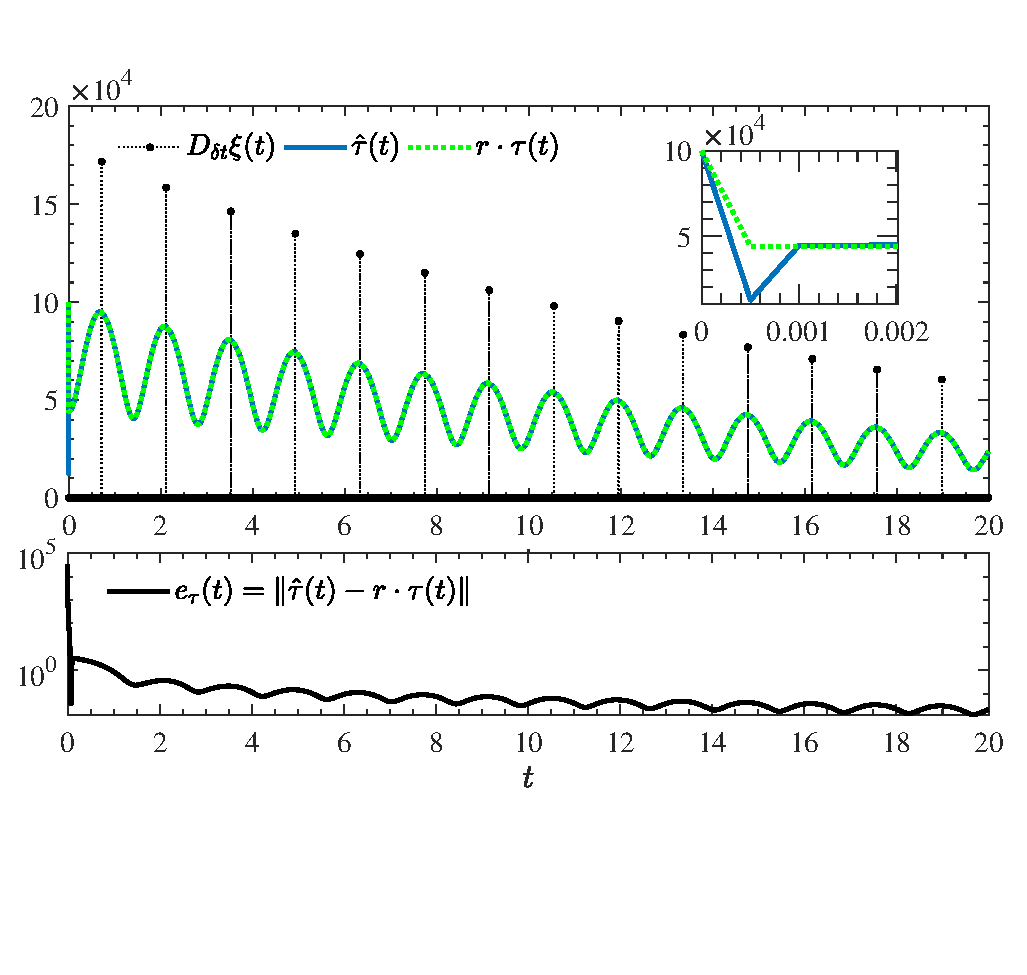
\includegraphics[trim={-10 0 0 0},scale=.75]{dderrnom}
	%\vspace*{-22mm}
	\caption[Nominal experiment: norm of the Euler derivative and estimated smoothness bound.]{Nominal experiment (no measurement noise). [Above] Norm of the Euler derivative $D_{\delta t}\x(t)$, (dotted black line and circe marker), estimated smoothness bound $\hat{\tau}(t)$ (blue solid line) and nominal smoothness bound $\tau(t)$ scaled by the arbitrary constant $r$. [Below] smoothness bound approximation error $e_{\tau}(t)$ (log scale).}
	\label{fig:dderrnom}
%vspace{-4.5mm}
\end{figure}
%
%
\begin{figure}[t!]
	%\vspace*{-18mm}
	\centering
	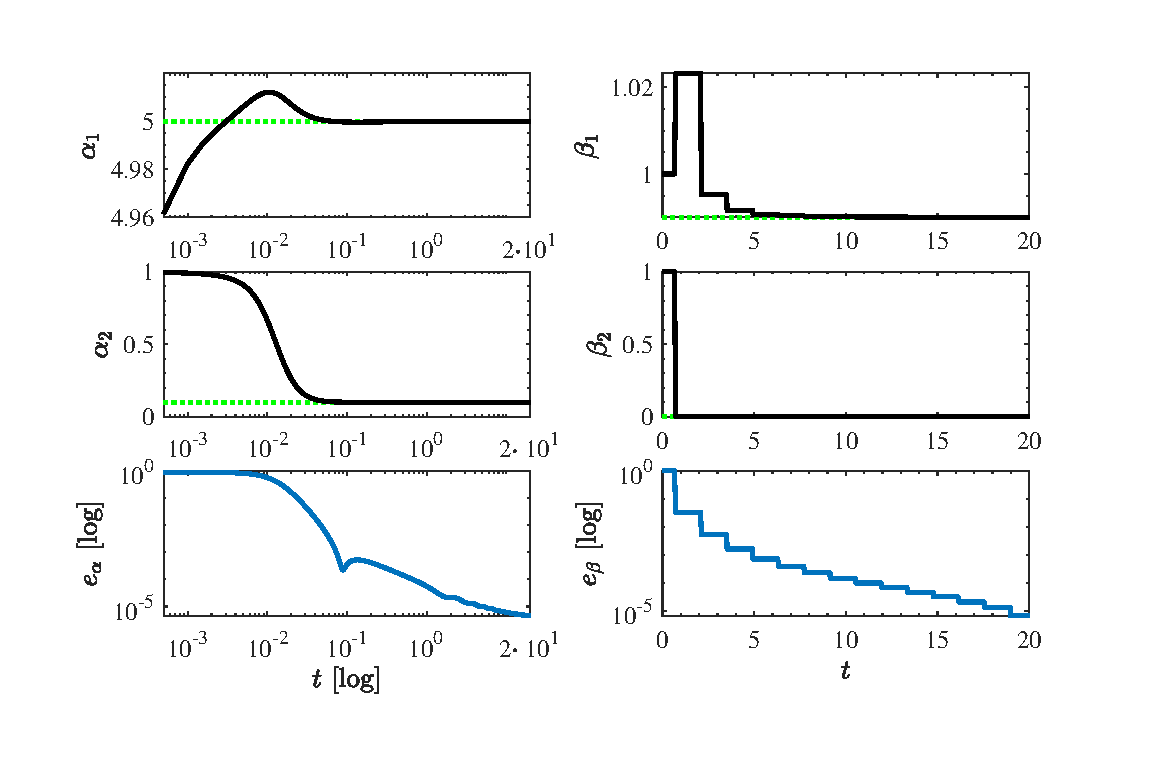
\includegraphics[trim={10 0 0 0},scale=.75]{parnom2}
	%\vspace*{-12mm}
	\caption[Nominal experiment: parameters estimation results.]{Nominal experiment (no measurement noise): parameters estimation results. [Left] Estimates of the parameters in $\bm{\alpha}$ and absolute estimation error $e_{\bm{\alpha}}(t)=\|\bm{\alpha}-\hat{\bm{\alpha}}(t)\|$ (below). [Right] Estimates of the parameters in $\bm{\beta}$ and absolute estimation error $e_{\bm{\beta}}(t)=\|\bm{\beta}-\hat{\bm{\beta}}(t)\|$ (below).}
	\label{fig:parnom}
	%\vspace{-7.5mm}
\end{figure}
%
\begin{figure}[t!]
	\centering
	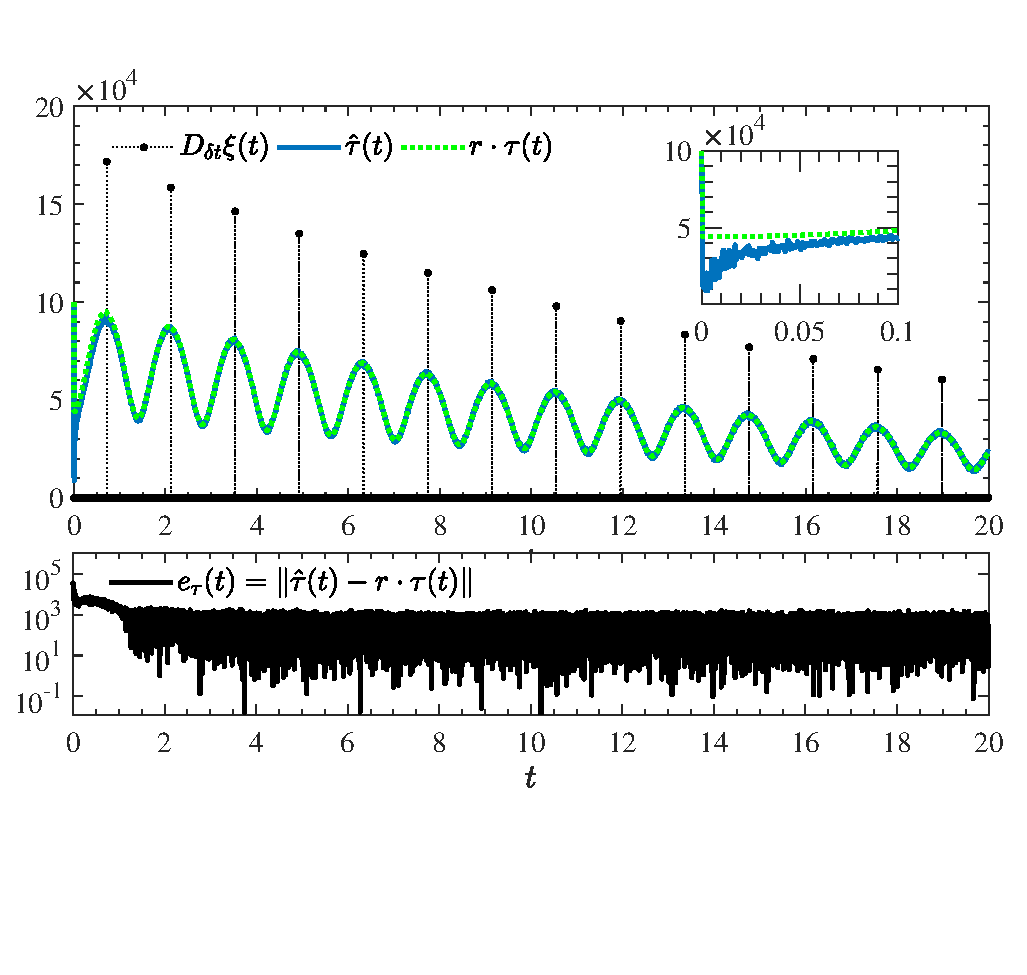
\includegraphics[trim={-10 0 0 0},scale=.75]{dderrnos2}
	%\vspace*{-22mm}
	\caption[Noisy experiment: norm of the Euler derivative and estimated smoothness bound.]{Noisy experiment (measurement noise standard deviation $\tilde{\sigma}_{\x}$=0.25). [Above] Norm of the Euler derivative $D_{\delta t}\x(t)$, (dotted black line and circle marker), estimated smoothness bound $\hat{\tau}(t)$ (blue solid line) and nominal smoothness bound $\tau(t)$ scaled by the arbitrary constant $r$. [Below] smoothness bound approximation error $e_{\tau}(t)$ (log scale).}
	\label{fig:dderrnos}
	%\vspace{-5mm}
\end{figure}
%
%
\begin{figure}[t!]
	\centering
	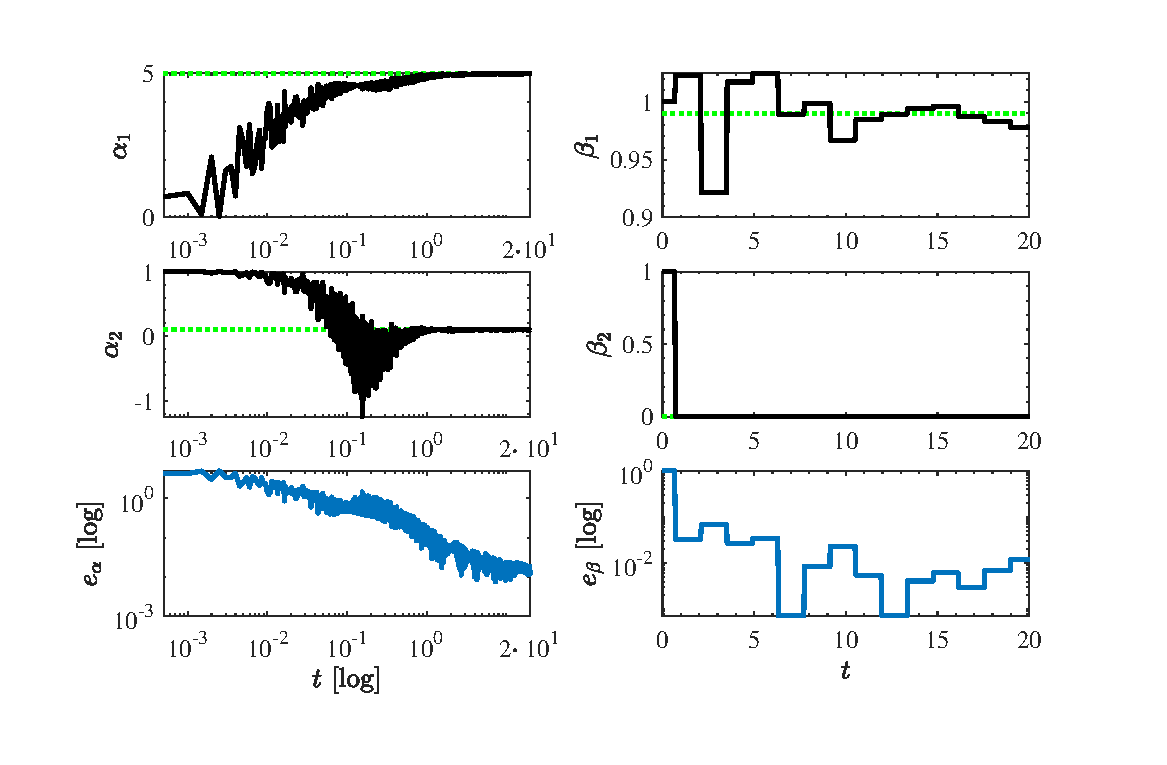
\includegraphics[trim={10 0 0 0},scale=0.75]{parnos}
	%\vspace*{-12mm}
	\caption[Noisy experiment: parameters estimation results.]{Noisy experiment (measurement noise standard deviation $\tilde{\sigma}_{\x}$=0.25): parameters estimation results. [Left] Estimates of the parameters in $\bm{\alpha}$ and absolute estimation error $e_{\bm{\alpha}}(t)=\|\bm{\alpha}-\hat{\bm{\alpha}}(t)\|$ (below). [Right] Estimates of the parameters in $\bm{\beta}$ and absolute estimation error $e_{\bm{\beta}}(t)=\|\bm{\beta}-\hat{\bm{\beta}}(t)\|$ (below).}
	\label{fig:parnos}
	%\vspace{-7mm}
\end{figure}

\clearpage
%%%%%%%%%%%%%%%%%%%%%%%%%%%%%%%%%%%%%%%%%%%%%%%%%%%%%%%%%%%%%%%%%%%%%%%%%%%%%%%%%%%%%%%%%%%
\section{Summary}\label{conc}
In this chapter, a new methodology for the identification of a class of hybrid dynamical systems, which evaluates the unknown parameters by employing a linear recursive estimator, has been proposed. The developed procedure is able to identify the state of the system and explicitly determine the flowing and jumping states. The method has been applied to a system falling in the category of hybrid port--Hamiltonian systems.
Here we have derived a systematic approach for the identification of hybrid dynamical systems, that to the best of authors' knowledge, is the first application of system identification methodologies to hybrid dynamical systems which can be analytically represented by Equation~\ref{eq:HS}.
Further development will include a more rigorous approach for the estimation of the smoothness bound without the need of any empirical coefficient, the exploration of alternative estimation schemes and a possible extension to the identification of \textit{hybrid inclusions}. Problems related to the non--convex approximation of the the flow and jump sets will also be regarded investigating new machine learning strategies.
%
%\chapter{Conclusion and Future Works}
\label{chap:conclusion_future_work}
\minitoc

\thispagestyle{empty}

\newpage
%%%%%%%%%%%%%%%%%%%%%%%%%%%%%%%%%%%%%%%%%%%%%%%%%%%%%%%%%%%%%%%%%%%%%%%%%%%%%%%
\section{Conclusion}
%The aim of this thesis is to build a glass confidence map for mobile robots using a LRF. The glass confidence map is supposed to first show glass on the map as occupied grids, and then indicate all the objects' probabilities of being glass. The application of the glass confidence map is to solve the problem that glass can not be shown on the map properly using standard SLAM algorithm, and the problem that robots cannot localize accurately using LRFs in glass environments.
%
%The above-mentioned problems, glass mapping problems and robot localization problems, are both caused by LRF's glass detection failure. LRFs can detect normal objects from almost all incident angles, while can only detect glass in limited incident angles, because of its transparency and reflectiveness. However, when building maps of environments, standard SLAM algorithms treat all the objects same and assume them can be detected from all angles. Consequently, glass are usually missing on the occupancy grid map generated. Additionally, while localizing using LRF in glass environments, the robot's localization accuracy is negatively influenced by the before-mentioned LRF's glass detection failure, because it causes mis-match between the robot's sensor measurements and the environment map. 
%
%Several previous research tried to solve the glass mapping problem and show glass on occupancy grid map using a LRF, as introduced in Chapter 2. Current state of the art solutions include recording objects' visible angle range and only use LRF scans within the range to map the glass, using multi-echo LRFs to classify and remove "erroneous" LRF scans showing glass is free space, as well as detecting glass by intensity peak and mark it on map directly. However, these methods either cannot help to solve the localization problem, need a special and more expensive sensor, or import path restrictions of the robot. 
%
%Facing all of the above-mentioned problems, this thesis proposed a novel solution, building a glass confidence map of the environment, which not only shows glass on the map, but also shows all the objects' glass probability. This glass confidence map solves the glass mapping problem, and also can be helpful in improving robots' localization accuracy in glass environment. 
%
%In order to build the glass confidence map, a novel method was proposed: first classify glass and non-glass objects, and then process glass and non-glass differently when building the map. The proposed method can classify glass, and works standard LRFs, without importing extra moving path restrictions, therefore it does not suffer from the previous research's problems. Specifically, the main contributions of this thesis are:
%
%\begin{itemize}
%	\item Proposing a new neural network based way to classify glass and non-glass objects using a LRF and calculate corresponding glass probability.
%	\item Proposing a new mapping method to incorporate the glass probability, filter out noise using two different thresholds, and build the glass confidence map.
%\end{itemize}
%
%The glass classifier, as introduced in Chapter 3, was built based on a neural network, with LRF's measured intensity, distance and incident angles as inputs, as well as glass probability as the output. The classifier was designed based on a proposed classification theory, that material features can be inferred by LRF intensity, distance and incident angle. This theory was analyzed theoretically and verified experimentally. While building the classifier, model-free machine learning method was chosen over model-based traditional statistical method, considering factors such as the insufficiency of the current theories as well as the unclearness of the LRF's signal processing mechanism. Among various machine learning methods, considering the problem complexity, neural network and SVM were chosen and compared using data collected from an office-like environment. As results, neural network was chosen to build the classifier, for the comparison results showed that it was comparably accurate and significantly faster than SVM. The neural network's structure was tuned to optimize in terms of speed and accuracy. At the end, a 2-layer the neural network, with 10 nodes on each layer was determined as the glass classifier used in this research. 
%
%In the proposed glass confidence map building method, as introduced in Chapter 4, two main processes are proposed to build the glass confidence map, using glass probability and other information from a standard SLAM algorithm. The first process is to register and update the glass probabilities onto a temporary map. Robot pose and LRF measurements' uncertainty were considered in the registration, and a Gaussian Filter was used to increase robustness. The second process is to filter out the noise of the temporal map and build the final glass confidence map. During this process, grids on the map were first classified into glass or non-glass, and then all the grids are filtered based on their occupancy probabilities, with applying a lower occupancy threshold to glass grids than to non-glass grids. Because glass has an inherent lower occupancy probability than non-glass objects, adopting two thresholds allows more glass to be shown correctly on the map.
%
%The whole glass confidence map building method was verified by experiments, as presented in Chapter 5. The proposed method was tested in two different office-like environments. The testing results showed that the proposed method can show more glass correctly on the map generated. In the dirty-glass environment, more glass, about 95.2\%, was shown correctly by the proposed method in the glass confidence map, while only 30.5\% of the glass was shown in the occupancy grid map by a standard SLAM algorithm. Besides, qualitative and quantitative analysis showed that the neural network classifier classified various types of glass and non-glass objects with high accuracy. Both the false positive and false negative error were less than 5\%. 
\clearpage

%%%%%%%%%%%%%%%%%%%%%%%%%%%%%%%%%%%%%%%%%%%%%%%%%%%%%%%%%%%%%%%%%%%%%%%%%%%%%%%
\section{Future Works}
%First, test the proposed mapping system further in various types of environments. The neural network classifier's performance mainly depends on the variety and quality of training dataset. Currently, the proposed method is trained and tested in only office-like environments. In future work, more experiments in various types of environments, such as home, shopping malls, airports, should be performed to test the classifier's ability and robustness. 
%
%Second, systematically improve the training dataset of the neural network classifier. There is the possibility that some new types of material, for example polyplastic or wood, are found cannot be classified correctly by the neural network classifier trained in this thesis. Though the problem can be solved easily by adding new material's sample into the training dataset, this is not a permanent solution. Instead, systematically improvements on the training dataset is needed to ensure the classifier's robustness, which needs a further study on the surface features' influence on LRF measured intensity.
%
%Last, use the glass confidence map to improve robot's localization accuracy in glass environments. As mentioned before, robot localization accuracy is negatively influenced by the mis-match between the LRF's measurements and map, and this problem can be solved by take the existence of glass into consideration while localizing. The glass confidence map provides the glass probabilities of each objects on the map, but the glass probability cannot be used directly by current localization algorithm. Therefore, improvements of current localization algorithm are needed to actually make use of the glass confidence map to improve robot's localization accuracy. 



%%%%%%%%%%%%%%%%%%%%%%%%%%%%%%%%%%%%%%%%%%%%%%%%%%%%%%%%%%%%%%%%%%%%%%%%%%%%%%%


%
%謝辞
%\chapter*{Acknowledgements}
\addcontentsline{toc}{chapter}{Acknowledgements}
\lhead[Acknowledgements]{}

\thispagestyle{empty}

\newpage
%%%%%%%%%%%%%%%%%%%%%%%%%%%%%%%%%%%%%%%%%%%%%%%%%%%%%%%%%%%%%%%%%%%%%%%%%%%%%%%
Now that I am writing the last few words of this thesis, I would like to thank all the people who contributed, in different ways, to this big achievement. 

First, I would like to thank my supervisor \textbf{Professor Hajime Asama} who made me part of his group and always guided me, teaching me how research works. His honest and sincere advice has been extremely important throughout all the path who lead me to this final result. Nevertheless, at a personal level, I want to express my outmost gratitude towards his to be my mentor and inspiration.

I would like to extend my sincere gratitude to the reviewers of my thesis, \textbf{Professor Hideki Kawakatsu} and \textbf{Lecturer Shunsuke Yoshimoto}. Their experience brought me insightful and keen suggestions which certainly helped in improving the quality of this thesis. Thank you very much, in advance.

Special thanks also to \textbf{Assaciate Professor Atsushi Yamashita} whose hardworking attitude and devotion to research gave me unvaluable teaching. Moreover, his timely, focused and objective advice always helped me taking the right direction at every turn. 

Although words are probably not enough, I have to extend my deepest gratitude to \textbf{Project Assistant Professor Angela Faragasso} for supervising me throughout all my Master course. I thank her for her patience, sincerity and friendship. 

In the same way, I would like to spend few words for \textbf{Dr. Federico Califano}, from the University of Twente. He has been my bachelor thesis supervisor in Bologna University and, since then, we became friends, starting a collaboration which certainly has been fundamental to the development of this thesis. His theoretical, yet insightful approach thought me a lot on how to output good research.

I would also like to extend my thanks to everyone at the Asama-Yamashita lab. In particular, to  \textbf{Project Associate Professor Yusuke Tamura}, \textbf{Assistant Professor Qi An}, \textbf{Project Assistant Professor Shota Chikushi}, \textbf{Technical Specialist Dr. Hiroshi Yamakawa}, \textbf{Visiting Researcher Dr. Alessandro Moro}, \textbf{JSPS Post Doctoral Research Sarthak Pathak} and all the students who form the wonderful team of staff at the Asama and Yamashita laboratories, and all other lab members for their constant support and academic/non-academic discussions.

Thanks also to \textbf{Ms. Maki Ishida}, \textbf{Ms. Negumi Nakamura} and special thanks to \textbf{Hisae Narushima} for always helping me, and everyone at the laboratory, in all administrative matters. 

Outside academia, I would like to thank all my family and friends who unconditionally supported me in every step of this path.

%Thanks to Ms. Rika Kojima, Ms. Megumi Nakamura, and special thanks to Ms. Hisae Narushima for always helping me, and everyone at the laboratory, in all administrative matters. Their counsel and prompt replies have been a great help these two years. 
%--\textit{Hamiltonian what?...}-- These are the words echoing in my mind writing the last few lines 
%of this strange thesis. While me and my dear friend Michael were coming back home from the Engineering campus of the \textit{Alma Mater Studiorum}, in a cold day of February 2017, he was   
%
%
%As I conclude the drafting of this thesis, my humor is a mixed bag of joy, confusion and commotion. During this strange and unexpected two years
%
%I would like to thank my second family, all the friends who have constantly been with me even if we are spread across the world: the ``\textit{Bomber}'' Riccardo, Mattia, ``\textit{Borbotta}'' Stefano,  ``\textit{Don}'' Carlo, the ``\textit{Botta}'' Alessandro and Matteo (who should answer the phone more). You have been helpful to survive here more than my broken Japanese. 





%As this thesis concludes, I would like to acknowledge and thank the guidance, cooperation and support of all the people who have helped my throughout the completion of this thesis.
%
%I would like to start by expressing my utmost gratitude towards my supervisor, professor Atsushi Yamashita, for giving me the chance to be part of his research group. I also want to thank him for his constant guidance and support on all aspects of academic research. Specially for the many insightful comments and suggestions that I have received during our regular meetings. All of which have shaped not only this thesis but also my approach towards research in general. 
%
%I am also thankful to the member of my thesis committee, professor Yasushi Umeda, for the time spent reading this thesis, his precise and accurate comments, and keen suggestions into how to improve this work.
%
%Special thanks to professor Hajime Asama, who together with professor Atsushi Yamashita, have always guided me since my arrival to Japan. My utmost thanks for always sparing some time to guide me and for all the the wise comments and suggestion I have always received. 
%
%I would like to also thank assistant professor Qi An, who has always helped me in several ways since my arrival to Japan. Thank to Dr. Alessandro Moro and Dr. Angela Faragasso, for their insightful and helpful suggestions on my research. Also many thanks to Dr. Hiroshi Yamakawa for helping me in all hardware related requirements I have had.
%
%I would like to extend my thanks to my seniors, specially to Mr. Renato Miyagusuku, on whose extensive knowledge in SLAM and related areas I have always relied on, as well as for always willingly helping me in the operation of robot, lab related procedures, researching life in general. Special thanks also to Dr. Sarthak Pathak, for all his comments and suggestions on my work, all the time he invested in reviewing this thesis, as well as the numerous witty jokes he shared with me. 
%
%I would also like to extend my thanks to everyone at the Asama-Yamashita lab, specially to everyone at the robotics' related group. In particular, many thanks to Mr. Hiroshi Higuchi for all the insightful comments and suggestions on my work, and for all the time spent reviewing this thesis. Also, special thanks to Mr. Younes Louhi, Mr. Ren Komatsu, Ms. Ningjia Yang, as well as former members Mr. Binbin Xu and Mr. Yuyang Shao for all research and non-research related discussions. Many thanks to former member Ms. Wei Sun, who was my tutors since my arrival to Japan. Thanks for helping me with the documents inside and outside the university. 
%
%Thanks to Ms. Rika Kojima, Ms. Megumi Nakamura, and special thanks to Ms. Hisae Narushima for always helping me, and everyone at the laboratory, in all administrative matters. Their counsel and prompt replies have been a great help these two years. 
%
%I also want to extend my thanks to the Iwatani Naoji Foundation for awarding me with the International Student Scholarship. Without their help, carrying my studies in Japan and the development of this thesis would not have been possible.
%
%In addition, I would like to thank my friends, those in my home country China and those I have made in Tokyo, for their help and support to my master study. Special thank to Ms. Yao Liu, who is my roommate in Tokyo and also one of my best friends, for the pleasant time we spent together and the meaningful conservations we had in our small house.  
%
%At the end, most importantly I would like to thank to my family, especially my parents, for their continuous and relentless support, which has made my live these last years so much more pleasurable.
%
%To all, thank you very much.

\begin{flushright}
August 2019, \enspace \textbf{Stefano Massaroli}
\end{flushright}

%%%%%%%%%%%%%%%%%%%%%%%%%%%%%%%%%%%%%%%%%%%%%%%%%%%%%%%%%%%%%%%%%%%%%%%%%%%%%%%

%%%%%%%%%%%%%%%%%%%%%%%%%%%%%%%%%%%%%%%%%%%%%%%%%%%%%%%%%%%%%%%%%%%%%%%%%%%%%%%
%%% Local Variables:
%%% mode: katex
%%% TeX-master: "../thesis"
%%% End:

%
%参考文献
%\chapter*{Bibliography}
\addcontentsline{toc}{chapter}{Bibliography}
\lhead[Bibliography]{}

\thispagestyle{empty}

\newpage

\begin{mythebibliography}{}
\bibitem[Ballard 1981]{Ballard1981}
\leavevmode \\
Ballard, Dana H.:
\newblock ``Generalizing the Hough transform to detect arbitrary shapes,''
\newblock Pattern recognition 13, no. 2 (1981): 111-122.
\\

\bibitem[Chong 2015]{chong2015}
\leavevmode \\
Chong, T. J., X. J. Tang, C. H. Leng, M. Yogeswaran, O. E. Ng, and Y. Z. Chong:
\newblock `` Sensor technologies and simultaneous localization and mapping (SLAM),''
\newblock Procedia Computer Science, Vol. 76, pp. 174-179, 2015.
\\ 

\bibitem[Diosi 2004]{dios2004}
\leavevmode \\
Diosi, Albert and Lindsay Kleeman:
\newblock ``Advanced sonar and laser range finder fusion for simultaneous localization and mapping,''
\newblock Proceedings of the 2004 IEEE International Conference on Intelligent Robots and Systems (IROS 2004), Vol. 2, pp. 1854-1859, IEEE, 2004.
\\ 
	
\bibitem[Foster 2013]{Foster2013}
\leavevmode \\
Foster, Paul, Zhenghong Sun, Jong Jin Park, and Benjamin Kuipers:
\newblock ``Visagge: Visible angle grid for glass environments,''
\newblock Proceedings of the 2013 IEEE International Conference on Robotics and Automation (ICRA 2013), pp. 2213-2220, IEEE, 2013.
\\ 
 
\bibitem[Giorgio 2007]{Giorgio2007}
\leavevmode \\
Giorgio Grisetti, Cyrill Stachniss, and Wolfram Burgard:
\newblock ``Improved Techniques for Grid Mapping with Rao-Blackwellized Particle Filters,''
\newblock IEEE Transactions on Robotics, Vol. 23, pp. 34-46, IEEE, 2007.
\\ 
 
\bibitem[Hancock 1999]{hancock1999}
\leavevmode \\
Hancock, John A:
\newblock ``Laser intensity-based obstacle detection and tracking,''
\newblock No. AAT 9936886 (UMI order no.). Carnegie Mellon University, 1999.
\\ 

\bibitem[Iwashina 2007]{iwashina2007}
\leavevmode \\
岩科進也, 山下淳, and 金子透:
\newblock ``レーザ・超音波センサ搭載移動ロボットによる透明物体を含む環境における 2 次元グリッド地図生成,''
\newblock 精密工学会画像応用技術専門委員会サマーセミナー 2007 テキスト, 伊豆, pp. 99-102, 2007.
\\ 

\bibitem[Juds 1988]{juds1988}
\leavevmode \\
Juds, Scott:
\newblock ``Photoelectric sensors and controls: selection and application,''
\newblock  Vol. 63. CRC Press, 1988.
\\ 

\bibitem[Nitzan 1977]{nitzan1977}
\leavevmode \\
Nitzan, David, Alfred E. Brain, and Richard O. Duda:
\newblock ``The measurement and use of registered reflectance and range data in scene analysis,''
\newblock  Proceedings of the IEEE Vol. 65, no. 2, pp. 206-220, 1977.
\\ 

\bibitem[Kawata 2005]{kawata2005}
\leavevmode \\
Kawata, Hirohiko, Akihisa Ohya, Shinichi Yuta, Wagle Santosh, and Toshihiro Mori:
\newblock ``Development of ultra-small lightweight optical range sensor system,''
\newblock  Proceedings of the 2005 IEEE/RSJ International Conference on Intelligent Robots and Systems (IROS 2005), pp. 1078-1083, IEEE, 2005.
\\ 

\bibitem[Klank 2011]{klank2011}
\leavevmode \\
Klank, Ulrich, Daniel Carton, and Michael Beetz:
\newblock ``Transparent object detection and reconstruction on a mobile platform,''
\newblock Proceedings of the 2013 IEEE International Conference on Robotics and Automation (ICRA 2011), pp. 5971-5978, IEEE, 2011.
\\ 

\bibitem[Kim 2016]{kim2016localization}
\leavevmode \\
Kim, Jiwoong, and Woojin Chung:
\newblock ``Localization of a mobile robot using a laser range finder in a glass-walled environment,''
\newblock IEEE Transactions on Industrial Electronics, Vol. 63, no. 6, pp. 3616-3627, IEEE, 2016.
\\ 
 
\bibitem[Kirchner 2009]{kirchner2009}
\leavevmode \\
Kirchner, Nathan, Dikai Liu, and Gamini Dissanayake:
\newblock ``Surface type classification with a laser range finder,''
\newblock IEEE Sensors Journal, Vol. 9, no. 9, pp. 1160-1168, IEEE, 2009.
\\ 

%\bibitem[Kirchner 2007]{kirchner2007}
%\leavevmode \\
%Kirchner, N. G., T. Taha, D. Liu, and G. Paul:
%\newblock ``Simultaneous material type classification and mapping data acquisition using a laser range finder,''
%\newblock Proceedings of the International Conference on Intelligent Technologies, 2007.
%\\ 

\bibitem[Koch 2017]{koch2017}
\leavevmode \\
Koch, Rainer, Stefan May, Patrick Murmann, and Andreas Nüchter:
\newblock ``Identification of transparent and specular reflective material in laser scans to discriminate affected measurements for faultless robotic SLAM,''
\newblock Robotics and Autonomous Systems, Vol. 87, pp. 296-312, 2017.
\\ 

\bibitem[Pedregosa 2011]{pedregosa2011}
\leavevmode \\
Pedregosa, Fabian, Gaël Varoquaux, Alexandre Gramfort, Vincent Michel, Bertrand Thirion, Olivier Grisel, Mathieu Blondel et al:
\newblock ``Scikit-learn: Machine learning in Python,''
\newblock Journal of Machine Learning Research, Vol. 12, pp. 2825-2830, 2011.
\\ 

\bibitem[Pedrotti 2017]{pedrotti2017}
\leavevmode \\
Pedrotti, Frank L., Leno M. Pedrotti, and Leno S. Pedrotti:
\newblock Introduction to Optics,
\newblock Cambridge University Press, 2017.
\\ 

\bibitem[Qing 2007]{qing2007}
\leavevmode \\
Qing, Zhaoshen, Baoping Ji, and Manuela Zude:
\newblock ``Predicting soluble solid content and firmness in apple fruit by means of laser light backscattering image analysis,''
\newblock Journal of Food Engineering 82, no. 1, pp. 58-67, 2007.
\\ 

\bibitem[Quigley 2009]{quigley2009}
\leavevmode \\
Quigley, Morgan, Ken Conley, Brian Gerkey, Josh Faust, Tully Foote, Jeremy Leibs, Rob Wheeler, and Andrew Y. Ng.:
\newblock ``ROS: an open-source Robot Operating System,''
\newblock In ICRA Workshop on Open Source Software, Vol. 3, no. 3.2, pp. 5, 2009.
\\ 

\bibitem[Ragheb 2002]{ragheb2002}
\leavevmode \\
Ragheb, Hossein, and Edwin R. Hancock:
\newblock ``Lambertian reflectance correction for rough and shiny surfaces,''
\newblock Proceedings of the 2002 International Conference on Image Processing, Vol. 2, pp. II-II, IEEE, 2002.
\\ 
 
\bibitem[Suykens 1999]{suykens1999}
\leavevmode \\
Suykens, Johan AK, and Joos Vandewalle:
\newblock ``Least squares support vector machine classifiers,''
\newblock Neural Processing Letters 9, no. 3, pp. 293-300, 1999.
\\ 

\bibitem[Tanaka 2012]{tanaka2012}
\leavevmode \\
Tanaka, Masahiro, and Keisuke Kochi:
\newblock ``Global localization of a mobile robot with a laser range scanner in the outdoor environment,''
\newblock Proceedings of the 2012 International Conference on Advanced Mechatronic Systems (ICAMechS 2012), pp. 69-74, IEEE, 2012.
\\ 

\bibitem[Thrun 2005]{thrun2005}
\leavevmode \\
Thrun, Sebastian, Wolfram Burgard, and Dieter Fox:
\newblock ``Probabilistic robotics,''
\newblock MIT press, 2005.
\\ 

\bibitem[Wang 2017]{wang2017}
\leavevmode \\
Wang, Xun, and JianGuo Wang:
\newblock ``Detecting glass in simultaneous localisation and mapping,''
\newblock Robotics and Autonomous Systems, Vol. 88, pp. 97-103, 2017.
\\ 

\bibitem[Zhang 2014]{zhang2014}
\leavevmode \\
Zhang, T., Z. J. Chong, B. Qin, J. G. M. Fu, S. Pendleton, and M. H. Ang:
\newblock ``Sensor fusion for localization, mapping and navigation in an indoor environment,''
\newblock Proceedings of the 2014 IEEE International Conference in Humanoid, Nanotechnology, Information Technology, Communication and Control, Environment and Management (HNICEM 2014), pp. 1-6, IEEE, 2014.
\\ 

% 
%\bibitem[Anderson 2002]{anderson2002building}
%\leavevmode \\
%Christopher~R Anderson, Theodore~S Rappaport, Kyung Bae, Alex Verstak, Naren  Ramakrishnan, William~H Tranter, Clifford Shaffer, Layne~T Watson, et~al:
%\newblock ``In-building wideband multipath characteristics at 2.5 and 60 ghz,''
%\newblock In \emph{Vehicular Technology Conference, 2002. Proceedings. VTC  2002-Fall. 2002 IEEE 56th}, volume~1, pages 97--101. IEEE, 2002.
%\\ 
% 
%\bibitem[Astr{\"o}m 2010]{astrom2010feedback}
%\leavevmode \\
%Karl~Johan Astr{\"o}m and Richard~M Murray:
%\newblock ``\emph{Feedback systems: an introduction for scientists and  engineers},''
%\newblock Princeton university press, 2010.
%\\ 

\end{mythebibliography}


%\nocite{*}
%\bibliographystyle{unsrt}
%\bibliographystyle{plain}
%\bibliographystyle{apalike} 
%\bibliographystyle{alpha} 

\bibliographystyle{engnatdin}
\bibliography{MasterThesis}

%研究業績
%\chapter*{Research Publications}
\addcontentsline{toc}{chapter}{Research Publications}
\lhead[Research Publications]{}

\thispagestyle{empty}

\newpage
%%%%%%%%%%%%%%%%%%%%%%%%%%%%%%%%%%%%%%%%%%%%%%%%%%%%%%%%%%%%%%%%%%%%%%%%%%%%%%%
\section*{Peer Reviewed Journal Papers}
\begin{enumerate}[{[}j1{]}]
	\item \textbf{Stefano Massaroli}, Federico Califano, Claudio Melchiorri, Atsushi Yamashita, and Hajime Asama: ``Port--Hamiltonian approach to asymptotic stabilisation of Lotka--Volterra equations.'', \textit{Scientific Reports, Nature}, 2018 (Submitted).
	%
	\item Jiaxu Wu, Hanwool Woo, Yusuke Tamura, Alessandro Moro, \textbf{Stefano Massaroli},
	Atsushi Yamashita, and Hajime Asama. ``Pedestrian trajectory prediction using BiRNN
	Encoder--Decoder Framework.'' \textit{Advanced Robotics}, 2019 (In print).
\end{enumerate}

\section*{Peer Reviewed Conference Papers}
\begin{enumerate}[{[}c1{]}]
\item \textbf{Stefano Massaroli}, Renato Miyagusuku, Federico Califano, Claudio Melchiorri, Atsushi Yamashita, and Hajime Asama: ``Recursive algebraic Frisch scheme: a particle--based approach'', \textit{IFAC PapersOnline}.
%
\item \textbf{Stefano Massaroli}, Renato Miyagusuku, Federico Califano, Angela Faragasso, Atsushi Yamashita, and Hajime Asama: ``A novel recursive linear estimator based on the Frisch scheme.'', \textit{Proceedings of the 2019 IFAC/IEEE Asian Control Conference}, Kitakyushu, Japan, June 2019.
%
\item \textbf{Stefano Massaroli}, Federico Califano, Angela Faragasso, Atsushi Yamashita, and
Hajime Asama. ``Iterative energy shaping of a ball--dribbling robot." \textit{2019 IFAC Workshop on Robot Control}, 2019. (Accepted)
%
\item \textbf{Stefano Massaroli}, Michael Poli, Federico Califano, Angela Faragasso, Atsushi Yamashita, and Hajime Asama: ``Port--Hamiltonian approach to neural network training.'' \textit{2019 Control and Decision Conference}, 2019. (Submitted)
%
\item \textbf{Stefano Massaroli}, Federico Califano, Angela Faragasso, Mattia Risiglione, Atsushi
Yamashita, and Hajime Asama. ``Identification of a class of hybrid dynamical systems.'' \textit{2019 Control and Decision Conference}, 2019. (Submitted)
%
\item \textbf{Stefano Massaroli}, Federico Califano, Angela Faragasso, Atsushi Yamashita, and Hajime Asama: ``Multistable energy shaping of linear time--invariant systems with hybrid mode selector.'' \textit{2020 IFAC World Congress}, 2019. (Submitted)
%
\end{enumerate}

\section*{Poster Presentations}
\begin{enumerate}[{[}p1{]}]
\item \textbf{Stefano Massaroli}, Atsushi Yamashita, and Hajime Asama: ``Hybrid energy--based control of a ball--dribbling robot'', 2019 IEEE/RSJ International Conference on Intelligent Robots and Systems (IROS 2019), 2019 (Submitted)%,Vancouver, Canada, September 2017.
\end{enumerate}

\section*{Oral Presentations}
\begin{enumerate}[{[}o1{]}]
	\item \textbf{Stefano Massaroli}, Atsushi Yamashita, and Hajime Asama: ``Biologically inspired control of robots for highly dynamic tasks'', Proceedings of the Tsinghua University- the University of Tokyo
	Joint Symposium on Multi-discipline, pp. 95, Beijing, China, March 2018.
\end{enumerate}
%
%付録
%\appendix
%\chapter*{Appendix}
\addcontentsline{toc}{chapter}{Appendix}
\lhead[Appendix]{}

\thispagestyle{empty}

\newpage

%%%%%%%%%%%%%%%%%%%%%%%%%%%%%%%%%%%%%%%%%%%%%%%%%%%%%%%%%%%%%%

\chapter{Set Theory and Differential Geometry}

%%%%%%%%%%%%%%%%%%%%%%%%%%%%%%%%%%%%%%%%%%%%%%%%%%%%%%%%%%%%%%%%%%%%%%%%%%%%%%
\section{Vector Spaces}\label{vectorspaces}

%\clearpage

%%%%%%%%%%%%%%%%%%%%%%%%%%%%%%%%%%%%%%%%%%%%%%%%%%%%%%%%%%%%%%%%%%%%%%%%%%%%%%
\section{Differential Geometry}
%%%%%%%%%%%%%%%%%%%%%
\subsection{Manifolds}
%%%%%%%%%%%%%%%%%%%%%%%%%%%%%%%%%%%%%%%%%%%%%%%%
\subsection{Tangent Spaces}\label{tangentspaces}
%%%%%%%%%%%%%%%%%%%%%%%%%%
\subsection{Distributions}
%
%
\chapter{Stability, Invariance and Passivity of Dynamical Systems}

%%%%%%%%%%%%%%%%%%%%%%%%%%%%%%%%%%%%%%%%%%%%%%%%%%%%%%%%%%%%%%%%%%%%%%%%%%%%%%
\section{Stability of Autonomous Systems}

%\clearpage

%%%%%%%%%%%%%%%%%%%%%%%%%%%%%%%%%%%%%%%%%%%%%%%%%%%%%%%%%%%%%%%%%%%%%%%%%%%%%%
\section{Invariance}

%\clearpage

%%%%%%%%%%%%%%%%%%%%%%%%%%%%%%%%%%%%%%%%%%%%%%%%%%%%%%%%%%%%%%%%%%%%%%%%%%%%%%
\section{Passivity}
%
%\subsection{Output Feedback Stabilization of Passive Systems}
%
\chapter{Set--Valued Mappings and Differential Inclusions}\label{chap:HSapp}
%%%%%%%%%%%%%%%%%%%%%%%%%%%%%%%%%%%%%%%%%%%%%%%%%%%%%%%%%%%%%%


%
%\chapter{Differential Geometry}

%\chapter{Set--Valued Mappings}


\cleardoublepage
%
% 論文の最後
%
\end{document}